% Options for packages loaded elsewhere
\PassOptionsToPackage{unicode}{hyperref}
\PassOptionsToPackage{hyphens}{url}
\PassOptionsToPackage{dvipsnames,svgnames,x11names}{xcolor}
%
\documentclass[
  letterpaper,
  DIV=11,
  numbers=noendperiod]{scrreprt}

\usepackage{amsmath,amssymb}
\usepackage{iftex}
\ifPDFTeX
  \usepackage[T1]{fontenc}
  \usepackage[utf8]{inputenc}
  \usepackage{textcomp} % provide euro and other symbols
\else % if luatex or xetex
  \usepackage{unicode-math}
  \defaultfontfeatures{Scale=MatchLowercase}
  \defaultfontfeatures[\rmfamily]{Ligatures=TeX,Scale=1}
\fi
\usepackage{lmodern}
\ifPDFTeX\else  
    % xetex/luatex font selection
\fi
% Use upquote if available, for straight quotes in verbatim environments
\IfFileExists{upquote.sty}{\usepackage{upquote}}{}
\IfFileExists{microtype.sty}{% use microtype if available
  \usepackage[]{microtype}
  \UseMicrotypeSet[protrusion]{basicmath} % disable protrusion for tt fonts
}{}
\makeatletter
\@ifundefined{KOMAClassName}{% if non-KOMA class
  \IfFileExists{parskip.sty}{%
    \usepackage{parskip}
  }{% else
    \setlength{\parindent}{0pt}
    \setlength{\parskip}{6pt plus 2pt minus 1pt}}
}{% if KOMA class
  \KOMAoptions{parskip=half}}
\makeatother
\usepackage{xcolor}
\setlength{\emergencystretch}{3em} % prevent overfull lines
\setcounter{secnumdepth}{5}
% Make \paragraph and \subparagraph free-standing
\ifx\paragraph\undefined\else
  \let\oldparagraph\paragraph
  \renewcommand{\paragraph}[1]{\oldparagraph{#1}\mbox{}}
\fi
\ifx\subparagraph\undefined\else
  \let\oldsubparagraph\subparagraph
  \renewcommand{\subparagraph}[1]{\oldsubparagraph{#1}\mbox{}}
\fi

\usepackage{color}
\usepackage{fancyvrb}
\newcommand{\VerbBar}{|}
\newcommand{\VERB}{\Verb[commandchars=\\\{\}]}
\DefineVerbatimEnvironment{Highlighting}{Verbatim}{commandchars=\\\{\}}
% Add ',fontsize=\small' for more characters per line
\usepackage{framed}
\definecolor{shadecolor}{RGB}{241,243,245}
\newenvironment{Shaded}{\begin{snugshade}}{\end{snugshade}}
\newcommand{\AlertTok}[1]{\textcolor[rgb]{0.68,0.00,0.00}{#1}}
\newcommand{\AnnotationTok}[1]{\textcolor[rgb]{0.37,0.37,0.37}{#1}}
\newcommand{\AttributeTok}[1]{\textcolor[rgb]{0.40,0.45,0.13}{#1}}
\newcommand{\BaseNTok}[1]{\textcolor[rgb]{0.68,0.00,0.00}{#1}}
\newcommand{\BuiltInTok}[1]{\textcolor[rgb]{0.00,0.23,0.31}{#1}}
\newcommand{\CharTok}[1]{\textcolor[rgb]{0.13,0.47,0.30}{#1}}
\newcommand{\CommentTok}[1]{\textcolor[rgb]{0.37,0.37,0.37}{#1}}
\newcommand{\CommentVarTok}[1]{\textcolor[rgb]{0.37,0.37,0.37}{\textit{#1}}}
\newcommand{\ConstantTok}[1]{\textcolor[rgb]{0.56,0.35,0.01}{#1}}
\newcommand{\ControlFlowTok}[1]{\textcolor[rgb]{0.00,0.23,0.31}{#1}}
\newcommand{\DataTypeTok}[1]{\textcolor[rgb]{0.68,0.00,0.00}{#1}}
\newcommand{\DecValTok}[1]{\textcolor[rgb]{0.68,0.00,0.00}{#1}}
\newcommand{\DocumentationTok}[1]{\textcolor[rgb]{0.37,0.37,0.37}{\textit{#1}}}
\newcommand{\ErrorTok}[1]{\textcolor[rgb]{0.68,0.00,0.00}{#1}}
\newcommand{\ExtensionTok}[1]{\textcolor[rgb]{0.00,0.23,0.31}{#1}}
\newcommand{\FloatTok}[1]{\textcolor[rgb]{0.68,0.00,0.00}{#1}}
\newcommand{\FunctionTok}[1]{\textcolor[rgb]{0.28,0.35,0.67}{#1}}
\newcommand{\ImportTok}[1]{\textcolor[rgb]{0.00,0.46,0.62}{#1}}
\newcommand{\InformationTok}[1]{\textcolor[rgb]{0.37,0.37,0.37}{#1}}
\newcommand{\KeywordTok}[1]{\textcolor[rgb]{0.00,0.23,0.31}{#1}}
\newcommand{\NormalTok}[1]{\textcolor[rgb]{0.00,0.23,0.31}{#1}}
\newcommand{\OperatorTok}[1]{\textcolor[rgb]{0.37,0.37,0.37}{#1}}
\newcommand{\OtherTok}[1]{\textcolor[rgb]{0.00,0.23,0.31}{#1}}
\newcommand{\PreprocessorTok}[1]{\textcolor[rgb]{0.68,0.00,0.00}{#1}}
\newcommand{\RegionMarkerTok}[1]{\textcolor[rgb]{0.00,0.23,0.31}{#1}}
\newcommand{\SpecialCharTok}[1]{\textcolor[rgb]{0.37,0.37,0.37}{#1}}
\newcommand{\SpecialStringTok}[1]{\textcolor[rgb]{0.13,0.47,0.30}{#1}}
\newcommand{\StringTok}[1]{\textcolor[rgb]{0.13,0.47,0.30}{#1}}
\newcommand{\VariableTok}[1]{\textcolor[rgb]{0.07,0.07,0.07}{#1}}
\newcommand{\VerbatimStringTok}[1]{\textcolor[rgb]{0.13,0.47,0.30}{#1}}
\newcommand{\WarningTok}[1]{\textcolor[rgb]{0.37,0.37,0.37}{\textit{#1}}}

\providecommand{\tightlist}{%
  \setlength{\itemsep}{0pt}\setlength{\parskip}{0pt}}\usepackage{longtable,booktabs,array}
\usepackage{multirow}
\usepackage{calc} % for calculating minipage widths
% Correct order of tables after \paragraph or \subparagraph
\usepackage{etoolbox}
\makeatletter
\patchcmd\longtable{\par}{\if@noskipsec\mbox{}\fi\par}{}{}
\makeatother
% Allow footnotes in longtable head/foot
\IfFileExists{footnotehyper.sty}{\usepackage{footnotehyper}}{\usepackage{footnote}}
\makesavenoteenv{longtable}
\usepackage{graphicx}
\makeatletter
\def\maxwidth{\ifdim\Gin@nat@width>\linewidth\linewidth\else\Gin@nat@width\fi}
\def\maxheight{\ifdim\Gin@nat@height>\textheight\textheight\else\Gin@nat@height\fi}
\makeatother
% Scale images if necessary, so that they will not overflow the page
% margins by default, and it is still possible to overwrite the defaults
% using explicit options in \includegraphics[width, height, ...]{}
\setkeys{Gin}{width=\maxwidth,height=\maxheight,keepaspectratio}
% Set default figure placement to htbp
\makeatletter
\def\fps@figure{htbp}
\makeatother

\KOMAoption{captions}{tableheading}
\makeatletter
\makeatother
\makeatletter
\@ifpackageloaded{bookmark}{}{\usepackage{bookmark}}
\makeatother
\makeatletter
\@ifpackageloaded{caption}{}{\usepackage{caption}}
\AtBeginDocument{%
\ifdefined\contentsname
  \renewcommand*\contentsname{Table of contents}
\else
  \newcommand\contentsname{Table of contents}
\fi
\ifdefined\listfigurename
  \renewcommand*\listfigurename{List of Figures}
\else
  \newcommand\listfigurename{List of Figures}
\fi
\ifdefined\listtablename
  \renewcommand*\listtablename{List of Tables}
\else
  \newcommand\listtablename{List of Tables}
\fi
\ifdefined\figurename
  \renewcommand*\figurename{Figure}
\else
  \newcommand\figurename{Figure}
\fi
\ifdefined\tablename
  \renewcommand*\tablename{Table}
\else
  \newcommand\tablename{Table}
\fi
}
\@ifpackageloaded{float}{}{\usepackage{float}}
\floatstyle{ruled}
\@ifundefined{c@chapter}{\newfloat{codelisting}{h}{lop}}{\newfloat{codelisting}{h}{lop}[chapter]}
\floatname{codelisting}{Listing}
\newcommand*\listoflistings{\listof{codelisting}{List of Listings}}
\makeatother
\makeatletter
\@ifpackageloaded{caption}{}{\usepackage{caption}}
\@ifpackageloaded{subcaption}{}{\usepackage{subcaption}}
\makeatother
\makeatletter
\@ifpackageloaded{tcolorbox}{}{\usepackage[skins,breakable]{tcolorbox}}
\makeatother
\makeatletter
\@ifundefined{shadecolor}{\definecolor{shadecolor}{rgb}{.97, .97, .97}}
\makeatother
\makeatletter
\makeatother
\makeatletter
\makeatother
\ifLuaTeX
  \usepackage{selnolig}  % disable illegal ligatures
\fi
\IfFileExists{bookmark.sty}{\usepackage{bookmark}}{\usepackage{hyperref}}
\IfFileExists{xurl.sty}{\usepackage{xurl}}{} % add URL line breaks if available
\urlstyle{same} % disable monospaced font for URLs
\hypersetup{
  pdftitle={Data Analytics in Finance},
  pdfauthor={Richard Herron},
  colorlinks=true,
  linkcolor={blue},
  filecolor={Maroon},
  citecolor={Blue},
  urlcolor={Blue},
  pdfcreator={LaTeX via pandoc}}

\title{Data Analytics in Finance}
\usepackage{etoolbox}
\makeatletter
\providecommand{\subtitle}[1]{% add subtitle to \maketitle
  \apptocmd{\@title}{\par {\large #1 \par}}{}{}
}
\makeatother
\subtitle{FINA 6333 for 2024 Spring}
\author{Richard Herron}
\date{}

\begin{document}
\maketitle
\ifdefined\Shaded\renewenvironment{Shaded}{\begin{tcolorbox}[borderline west={3pt}{0pt}{shadecolor}, interior hidden, frame hidden, sharp corners, breakable, enhanced, boxrule=0pt]}{\end{tcolorbox}}\fi

\renewcommand*\contentsname{Table of contents}
{
\hypersetup{linkcolor=}
\setcounter{tocdepth}{1}
\tableofcontents
}
\bookmarksetup{startatroot}

\hypertarget{welcome}{%
\chapter*{Welcome!}\label{welcome}}
\addcontentsline{toc}{chapter}{Welcome!}

\markboth{Welcome!}{Welcome!}

Welcome to FINA 6333 for Spring 2024 at the D'Amore-McKim School of
Business at Northeastern University!

For each course topic, we will have one notebook for its lecture and one
for its in-class practice exercises. I will maintain these notebooks
here because Canvas does not render notebooks. I will maintain
everything else on Canvas (e.g., announcements, discussions, grades,
etc.).

You have three choices to download or run these notebooks:

\begin{enumerate}
\def\labelenumi{\arabic{enumi}.}
\tightlist
\item
  Download them from our shared folder on
  \href{https://northeastern-my.sharepoint.com/:f:/g/personal/r_herron_northeastern_edu/Ekn1N5nzwXFDpezlTLQqLd8BBQcfvgDCkE9OgdIffHR8Cw?e=t8Dqa3}{OneDrive}
  (or click the cloud icon in the left sidebar)
\item
  Download them from our Notebooks folder on
  \href{https://github.com/richard-herron/fina-6333-2024-spring}{GitHub}
  (or click the octo-cat icon in the left sidebar)
\item
  Open them on
  \href{http://colab.research.google.com/github/richard-herron/fina-6333-2024-spring/}{Google
  Colab} (or click the Google icon in the left sidebar)
\end{enumerate}

\part{Week 1}

\hypertarget{mckinney-chapter-2---python-language-basics-ipython-and-jupyter-notebooks}{%
\chapter{McKinney Chapter 2 - Python Language Basics, IPython, and
Jupyter
Notebooks}\label{mckinney-chapter-2---python-language-basics-ipython-and-jupyter-notebooks}}

\hypertarget{introduction}{%
\section{Introduction}\label{introduction}}

We must understand the basics of Python before we can use it to analyze
financial data. Chapter 2 of Wes McKinney's
\href{https://wesmckinney.com/book/}{\emph{Python for Data Analysis}}
provides a crash course in Python's syntax, and chapter 3 provides a
crash course in Python's built-in data structures. This notebook focuses
on the ``Python Language Basics'' in section 2.3, which covers language
semantics, scalar types, and control flow.

\textbf{\emph{Note:}} Indented block quotes are from McKinney unless
otherwise indicated. The section numbers here differ from McKinney
because we will only discuss some topics.

\hypertarget{language-semantics}{%
\section{Language Semantics}\label{language-semantics}}

\hypertarget{indentation-not-braces}{%
\subsection{Indentation, not braces}\label{indentation-not-braces}}

\begin{quote}
Python uses whitespace (tabs or spaces) to structure code instead of
using braces as in many other languages like R, C++, Java, and Perl.
\end{quote}

\textbf{\emph{So, spaces are more than cosmetic in Python.}} For
non-Python programmers, white space is often Python's defining feature.
Here is a for loop with an if block that shows how Python uses white
space.

\begin{Shaded}
\begin{Highlighting}[]
\NormalTok{array }\OperatorTok{=}\NormalTok{ [}\DecValTok{1}\NormalTok{, }\DecValTok{2}\NormalTok{, }\DecValTok{3}\NormalTok{]}
\NormalTok{pivot }\OperatorTok{=} \DecValTok{2}
\NormalTok{less }\OperatorTok{=}\NormalTok{ []}
\NormalTok{greater }\OperatorTok{=}\NormalTok{ []}

\ControlFlowTok{for}\NormalTok{ x }\KeywordTok{in}\NormalTok{ array:}
    \ControlFlowTok{if}\NormalTok{ x }\OperatorTok{\textless{}}\NormalTok{ pivot:}
        \BuiltInTok{print}\NormalTok{(}\SpecialStringTok{f\textquotesingle{}}\SpecialCharTok{\{}\NormalTok{x}\SpecialCharTok{\}}\SpecialStringTok{ is less than }\SpecialCharTok{\{}\NormalTok{pivot}\SpecialCharTok{\}}\SpecialStringTok{\textquotesingle{}}\NormalTok{)}
\NormalTok{        less.append(x)        }
    \ControlFlowTok{else}\NormalTok{:}
        \BuiltInTok{print}\NormalTok{(}\SpecialStringTok{f\textquotesingle{}}\SpecialCharTok{\{}\NormalTok{x}\SpecialCharTok{\}}\SpecialStringTok{ is NOT less than }\SpecialCharTok{\{}\NormalTok{pivot}\SpecialCharTok{\}}\SpecialStringTok{\textquotesingle{}}\NormalTok{)}
\NormalTok{        greater.append(x)}
\end{Highlighting}
\end{Shaded}

\begin{verbatim}
1 is less than 2
2 is NOT less than 2
3 is NOT less than 2
\end{verbatim}

\begin{Shaded}
\begin{Highlighting}[]
\NormalTok{less}
\end{Highlighting}
\end{Shaded}

\begin{verbatim}
[1]
\end{verbatim}

\begin{Shaded}
\begin{Highlighting}[]
\NormalTok{greater}
\end{Highlighting}
\end{Shaded}

\begin{verbatim}
[2, 3]
\end{verbatim}

\textbf{\emph{Note:}} We will use f-string print statements wherever we
can. These f-string print statements are easy to use, and I do not want
to teach old approaches when the new ones are better.

\hypertarget{comments}{%
\subsection{Comments}\label{comments}}

\begin{quote}
Any text preceded by the hash mark (pound sign) \# is ignored by the
Python interpreter. This is often used to add comments to code. At times
you may also want to exclude certain blocks of code without deleting
them.
\end{quote}

The Python interpreter ignores any code after a hash mark \texttt{\#} on
a given line. We can quickly comment/un-comment lines of code with the
\texttt{\textless{}Ctrl\textgreater{}-/} shortcut.

\begin{Shaded}
\begin{Highlighting}[]
\CommentTok{\# We often use comments to leave notes for future us (or co{-}workers)}
\CommentTok{\# 5 + 5}
\end{Highlighting}
\end{Shaded}

\hypertarget{function-and-object-method-calls}{%
\subsection{Function and object method
calls}\label{function-and-object-method-calls}}

\begin{quote}
You call functions using parentheses and passing zero or more arguments,
optionally assigning the returned value to a variable:

\begin{Shaded}
\begin{Highlighting}[]
\NormalTok{    result }\OperatorTok{=}\NormalTok{ f(x, y, z)}
\NormalTok{    g()}
\end{Highlighting}
\end{Shaded}

Almost every object in Python has attached functions, known as methods,
that have access to the object's internal contents. You can call them
using the following \textgreater{} syntax:

\begin{Shaded}
\begin{Highlighting}[]
\NormalTok{    obj.some\_method(x, y, z)}
\end{Highlighting}
\end{Shaded}

Functions can take both positional and keyword arguments:

\begin{Shaded}
\begin{Highlighting}[]
\NormalTok{    result }\OperatorTok{=}\NormalTok{ f(a, b, c, d}\OperatorTok{=}\DecValTok{5}\NormalTok{, e}\OperatorTok{=}\StringTok{\textquotesingle{}foo\textquotesingle{}}\NormalTok{)}
\end{Highlighting}
\end{Shaded}

More on this later.
\end{quote}

We can write a function that adds two numbers.

\begin{Shaded}
\begin{Highlighting}[]
\KeywordTok{def}\NormalTok{ add\_numbers(a, b):}
    \ControlFlowTok{return}\NormalTok{ a }\OperatorTok{+}\NormalTok{ b}
\end{Highlighting}
\end{Shaded}

\begin{Shaded}
\begin{Highlighting}[]
\OperatorTok{\%}\NormalTok{who}
\end{Highlighting}
\end{Shaded}

\begin{verbatim}
add_numbers  array   greater     less    pivot   x   
\end{verbatim}

\begin{Shaded}
\begin{Highlighting}[]
\NormalTok{add\_numbers(}\DecValTok{5}\NormalTok{, }\DecValTok{5}\NormalTok{)}
\end{Highlighting}
\end{Shaded}

\begin{verbatim}
10
\end{verbatim}

We can write a function that adds two strings separated by a space.

\begin{Shaded}
\begin{Highlighting}[]
\KeywordTok{def}\NormalTok{ add\_strings(a, b):}
    \ControlFlowTok{return}\NormalTok{ a }\OperatorTok{+} \StringTok{\textquotesingle{} \textquotesingle{}} \OperatorTok{+}\NormalTok{ b}
\end{Highlighting}
\end{Shaded}

\begin{Shaded}
\begin{Highlighting}[]
\OperatorTok{\%}\NormalTok{who}
\end{Highlighting}
\end{Shaded}

\begin{verbatim}
add_numbers  add_strings     array   greater     less    pivot   x   
\end{verbatim}

\begin{Shaded}
\begin{Highlighting}[]
\NormalTok{add\_strings(}\StringTok{\textquotesingle{}5\textquotesingle{}}\NormalTok{, }\StringTok{\textquotesingle{}5\textquotesingle{}}\NormalTok{)}
\end{Highlighting}
\end{Shaded}

\begin{verbatim}
'5 5'
\end{verbatim}

\textbf{\emph{What is the difference between \texttt{print()} and
\texttt{return}?}} \texttt{print()} returns its arguments to the console
or ``standard output'', whereas \texttt{return} returns its argument as
an output we can assign to variables. In the example below, we use the
\texttt{return} line to assign the output of \texttt{add\_string\_2()}
to the variable \texttt{return\_from\_add\_strings\_2}. The
\texttt{print()} line prints to the console or ``standard output'', but
its output is not assigned or captured.

\begin{Shaded}
\begin{Highlighting}[]
\KeywordTok{def}\NormalTok{ add\_strings\_2(a, b):}
\NormalTok{    string\_to\_print }\OperatorTok{=}\NormalTok{ a }\OperatorTok{+} \StringTok{\textquotesingle{} \textquotesingle{}} \OperatorTok{+}\NormalTok{ b }\OperatorTok{+} \StringTok{\textquotesingle{} (this is from the print statement)\textquotesingle{}}
\NormalTok{    string\_to\_return }\OperatorTok{=}\NormalTok{ a }\OperatorTok{+} \StringTok{\textquotesingle{} \textquotesingle{}} \OperatorTok{+}\NormalTok{ b }\OperatorTok{+} \StringTok{\textquotesingle{} (this is from the return statement)\textquotesingle{}}
    \BuiltInTok{print}\NormalTok{(string\_to\_print)}
    \ControlFlowTok{return}\NormalTok{ string\_to\_return}
\end{Highlighting}
\end{Shaded}

\begin{Shaded}
\begin{Highlighting}[]
\NormalTok{returned }\OperatorTok{=}\NormalTok{ add\_strings\_2(}\StringTok{\textquotesingle{}5\textquotesingle{}}\NormalTok{, }\StringTok{\textquotesingle{}5\textquotesingle{}}\NormalTok{)}
\end{Highlighting}
\end{Shaded}

\begin{verbatim}
5 5 (this is from the print statement)
\end{verbatim}

\begin{Shaded}
\begin{Highlighting}[]
\NormalTok{returned}
\end{Highlighting}
\end{Shaded}

\begin{verbatim}
'5 5 (this is from the return statement)'
\end{verbatim}

\hypertarget{variables-and-argument-passing}{%
\subsection{Variables and argument
passing}\label{variables-and-argument-passing}}

\begin{quote}
When assigning a variable (or name) in Python, you are creating a
reference to the object on the righthand side of the equals sign.
\end{quote}

\begin{Shaded}
\begin{Highlighting}[]
\NormalTok{a }\OperatorTok{=}\NormalTok{ [}\DecValTok{1}\NormalTok{, }\DecValTok{2}\NormalTok{, }\DecValTok{3}\NormalTok{]}
\end{Highlighting}
\end{Shaded}

\begin{Shaded}
\begin{Highlighting}[]
\NormalTok{a}
\end{Highlighting}
\end{Shaded}

\begin{verbatim}
[1, 2, 3]
\end{verbatim}

If we assign \texttt{a} to a new variable \texttt{b}, both \texttt{a}
and \texttt{b} refer to the \emph{same} object. This same object is the
list \texttt{{[}1,\ 2,\ 3{]}}. If we change \texttt{a}, we also change
\texttt{b}, because these variables or names refer to the \emph{same}
object.

\begin{Shaded}
\begin{Highlighting}[]
\NormalTok{b }\OperatorTok{=}\NormalTok{ a}
\end{Highlighting}
\end{Shaded}

\begin{Shaded}
\begin{Highlighting}[]
\NormalTok{b}
\end{Highlighting}
\end{Shaded}

\begin{verbatim}
[1, 2, 3]
\end{verbatim}

\textbf{\emph{Variables \texttt{a} and \texttt{b} refer to the same
object, a list \texttt{{[}1,\ 2,\ 3{]}}.}} We will learn more about
lists (and tuples and dictionaries) in chapter 3 of McKinney.

\begin{Shaded}
\begin{Highlighting}[]
\NormalTok{a }\KeywordTok{is}\NormalTok{ b}
\end{Highlighting}
\end{Shaded}

\begin{verbatim}
True
\end{verbatim}

\textbf{\emph{If we modify \texttt{a} by appending a 4, we change
\texttt{b} because \texttt{a} and \texttt{b} refer to the same list.}}

\begin{Shaded}
\begin{Highlighting}[]
\NormalTok{a.append(}\DecValTok{4}\NormalTok{)}
\end{Highlighting}
\end{Shaded}

\begin{Shaded}
\begin{Highlighting}[]
\NormalTok{a}
\end{Highlighting}
\end{Shaded}

\begin{verbatim}
[1, 2, 3, 4]
\end{verbatim}

\begin{Shaded}
\begin{Highlighting}[]
\NormalTok{b}
\end{Highlighting}
\end{Shaded}

\begin{verbatim}
[1, 2, 3, 4]
\end{verbatim}

\begin{Shaded}
\begin{Highlighting}[]
\NormalTok{a }\KeywordTok{is}\NormalTok{ b}
\end{Highlighting}
\end{Shaded}

\begin{verbatim}
True
\end{verbatim}

\textbf{\emph{Likewise, if we modify \texttt{b} by appending a 5, we
change \texttt{a}, too!}}

\begin{Shaded}
\begin{Highlighting}[]
\NormalTok{b.append(}\DecValTok{5}\NormalTok{)}
\end{Highlighting}
\end{Shaded}

\begin{Shaded}
\begin{Highlighting}[]
\NormalTok{a}
\end{Highlighting}
\end{Shaded}

\begin{verbatim}
[1, 2, 3, 4, 5]
\end{verbatim}

\begin{Shaded}
\begin{Highlighting}[]
\NormalTok{b}
\end{Highlighting}
\end{Shaded}

\begin{verbatim}
[1, 2, 3, 4, 5]
\end{verbatim}

\begin{Shaded}
\begin{Highlighting}[]
\NormalTok{a }\KeywordTok{is}\NormalTok{ b}
\end{Highlighting}
\end{Shaded}

\begin{verbatim}
True
\end{verbatim}

The behavior is useful but a double-edged sword!
\href{https://nedbatchelder.com/text/names.html}{Here} is a deeper
discussion of this behavior.

\hypertarget{dynamic-references-strong-types}{%
\subsection{Dynamic references, strong
types}\label{dynamic-references-strong-types}}

\begin{quote}
In contrast with many compiled languages, such as Java and C++, object
references in Python have no type associated with them.
\end{quote}

In Python,

\begin{enumerate}
\def\labelenumi{\arabic{enumi}.}
\tightlist
\item
  We do not declare variables and their types
\item
  We can change variables' types because variables are only names that
  refer to objects
\end{enumerate}

\emph{Dynamic references} mean we can reassign a variable to a new
object in Python. For example, we can reassign \texttt{a} from a list to
an integer to a string.

\begin{Shaded}
\begin{Highlighting}[]
\NormalTok{a}
\end{Highlighting}
\end{Shaded}

\begin{verbatim}
[1, 2, 3, 4, 5]
\end{verbatim}

\begin{Shaded}
\begin{Highlighting}[]
\BuiltInTok{type}\NormalTok{(a)}
\end{Highlighting}
\end{Shaded}

\begin{verbatim}
list
\end{verbatim}

\begin{Shaded}
\begin{Highlighting}[]
\NormalTok{a }\OperatorTok{=} \DecValTok{5}
\BuiltInTok{type}\NormalTok{(a)}
\end{Highlighting}
\end{Shaded}

\begin{verbatim}
int
\end{verbatim}

\begin{Shaded}
\begin{Highlighting}[]
\NormalTok{a }\OperatorTok{=} \StringTok{\textquotesingle{}foo\textquotesingle{}}
\BuiltInTok{type}\NormalTok{(a)}
\end{Highlighting}
\end{Shaded}

\begin{verbatim}
str
\end{verbatim}

\emph{Strong types} mean Python typically will not convert object types.
For example, the code returns either
\texttt{\textquotesingle{}55\textquotesingle{}} as a string or
\texttt{10} as an integer in many programming languages. However,
\texttt{\textquotesingle{}5\textquotesingle{}\ +\ 5} returns an error in
Python.

\begin{Shaded}
\begin{Highlighting}[]
\CommentTok{\# \textquotesingle{}5\textquotesingle{} + 5}
\end{Highlighting}
\end{Shaded}

However, Python implicitly converts integers to floats.

\begin{Shaded}
\begin{Highlighting}[]
\NormalTok{a }\OperatorTok{=} \FloatTok{4.5}
\NormalTok{b }\OperatorTok{=} \DecValTok{2}
\BuiltInTok{print}\NormalTok{(}\SpecialStringTok{f\textquotesingle{}a is }\SpecialCharTok{\{}\BuiltInTok{type}\NormalTok{(a)}\SpecialCharTok{\}}\SpecialStringTok{, b is }\SpecialCharTok{\{}\BuiltInTok{type}\NormalTok{(b)}\SpecialCharTok{\}}\SpecialStringTok{\textquotesingle{}}\NormalTok{)}
\NormalTok{a }\OperatorTok{/}\NormalTok{ b}
\end{Highlighting}
\end{Shaded}

\begin{verbatim}
a is <class 'float'>, b is <class 'int'>
\end{verbatim}

\begin{verbatim}
2.25
\end{verbatim}

In the previous code cell:

\begin{enumerate}
\def\labelenumi{\arabic{enumi}.}
\tightlist
\item
  The `a is \ldots{}' output prints because of the explicit
  \texttt{print()} function call
\item
  The output of \texttt{a\ /\ b} prints (or displays) because it is the
  last line in the code cell
\end{enumerate}

If we want integer division (or floor division), we have to use
\texttt{//}.

\begin{Shaded}
\begin{Highlighting}[]
\DecValTok{5} \OperatorTok{//} \DecValTok{2}
\end{Highlighting}
\end{Shaded}

\begin{verbatim}
2
\end{verbatim}

\begin{Shaded}
\begin{Highlighting}[]
\DecValTok{5} \OperatorTok{/} \DecValTok{2}
\end{Highlighting}
\end{Shaded}

\begin{verbatim}
2.5
\end{verbatim}

\hypertarget{attributes-and-methods}{%
\subsection{Attributes and methods}\label{attributes-and-methods}}

We can use tab completion to list attributes (characteristics stored
inside objects) and methods (functions associated with objects).

\begin{Shaded}
\begin{Highlighting}[]
\NormalTok{a }\OperatorTok{=} \StringTok{\textquotesingle{}foo\textquotesingle{}}
\end{Highlighting}
\end{Shaded}

\begin{Shaded}
\begin{Highlighting}[]
\NormalTok{a.capitalize()}
\end{Highlighting}
\end{Shaded}

\begin{verbatim}
'Foo'
\end{verbatim}

\begin{Shaded}
\begin{Highlighting}[]
\NormalTok{a.upper().lower()}
\end{Highlighting}
\end{Shaded}

\begin{verbatim}
'foo'
\end{verbatim}

\hypertarget{imports}{%
\subsection{Imports}\label{imports}}

\begin{quote}
In Python a module is simply a file with the .py extension containing
Python code.
\end{quote}

We can import with \texttt{import} statements, which have several
syntaxes. The basic syntax uses the module name as the prefix to
separate module items from our current namespace.

\begin{Shaded}
\begin{Highlighting}[]
\ImportTok{import}\NormalTok{ pandas}
\end{Highlighting}
\end{Shaded}

The \texttt{import\ as} syntax lets us define an abbreviated prefix.

\begin{Shaded}
\begin{Highlighting}[]
\ImportTok{import}\NormalTok{ pandas }\ImportTok{as}\NormalTok{ pd}
\end{Highlighting}
\end{Shaded}

We can also import one or more items from a package into our namespace
with the following syntaxes.

\begin{Shaded}
\begin{Highlighting}[]
\ImportTok{from}\NormalTok{ pandas }\ImportTok{import}\NormalTok{ DataFrame}
\end{Highlighting}
\end{Shaded}

\begin{Shaded}
\begin{Highlighting}[]
\ImportTok{from}\NormalTok{ pandas }\ImportTok{import}\NormalTok{ DataFrame }\ImportTok{as}\NormalTok{ df}
\end{Highlighting}
\end{Shaded}

\hypertarget{binary-operators-and-comparisons}{%
\subsection{Binary operators and
comparisons}\label{binary-operators-and-comparisons}}

Binary operators work like Excel.

\begin{Shaded}
\begin{Highlighting}[]
\DecValTok{5} \OperatorTok{{-}} \DecValTok{7}
\end{Highlighting}
\end{Shaded}

\begin{verbatim}
-2
\end{verbatim}

\begin{Shaded}
\begin{Highlighting}[]
\DecValTok{12} \OperatorTok{+} \FloatTok{21.5}
\end{Highlighting}
\end{Shaded}

\begin{verbatim}
33.5
\end{verbatim}

\begin{Shaded}
\begin{Highlighting}[]
\DecValTok{5} \OperatorTok{\textless{}=} \DecValTok{2}
\end{Highlighting}
\end{Shaded}

\begin{verbatim}
False
\end{verbatim}

We can operate during an assignment to avoid two names referring to the
same object.

\begin{Shaded}
\begin{Highlighting}[]
\NormalTok{a }\OperatorTok{=}\NormalTok{ [}\DecValTok{1}\NormalTok{, }\DecValTok{2}\NormalTok{, }\DecValTok{3}\NormalTok{]}
\NormalTok{b }\OperatorTok{=}\NormalTok{ a}
\NormalTok{c }\OperatorTok{=} \BuiltInTok{list}\NormalTok{(a)}
\end{Highlighting}
\end{Shaded}

\begin{Shaded}
\begin{Highlighting}[]
\NormalTok{a }\KeywordTok{is}\NormalTok{ b}
\end{Highlighting}
\end{Shaded}

\begin{verbatim}
True
\end{verbatim}

\begin{Shaded}
\begin{Highlighting}[]
\NormalTok{a }\KeywordTok{is}\NormalTok{ c}
\end{Highlighting}
\end{Shaded}

\begin{verbatim}
False
\end{verbatim}

Here \texttt{a} and \texttt{c} have the same \emph{values} but are not
the same object!

\begin{Shaded}
\begin{Highlighting}[]
\NormalTok{a }\OperatorTok{==}\NormalTok{ c}
\end{Highlighting}
\end{Shaded}

\begin{verbatim}
True
\end{verbatim}

\begin{Shaded}
\begin{Highlighting}[]
\NormalTok{a }\KeywordTok{is} \KeywordTok{not}\NormalTok{ c}
\end{Highlighting}
\end{Shaded}

\begin{verbatim}
True
\end{verbatim}

In Python, \texttt{=} is the assignment operator, \texttt{==} tests
equality, and \texttt{!=} tests inequality (\texttt{!=} in Python is
like \texttt{\textless{}\textgreater{}} in Excel).

\begin{Shaded}
\begin{Highlighting}[]
\NormalTok{a }\OperatorTok{==}\NormalTok{ c}
\end{Highlighting}
\end{Shaded}

\begin{verbatim}
True
\end{verbatim}

\begin{Shaded}
\begin{Highlighting}[]
\NormalTok{a }\OperatorTok{!=}\NormalTok{ c}
\end{Highlighting}
\end{Shaded}

\begin{verbatim}
False
\end{verbatim}

\texttt{a} and \texttt{c} have the same values but reference different
objects in memory.

\textbf{\emph{Table 2-1}} from McKinney summarizes the binary operators.

\begin{itemize}
\tightlist
\item
  \texttt{a\ +\ b} : Add a and b
\item
  \texttt{a\ -\ b} : Subtract b from a
\item
  \texttt{a\ *\ b} : Multiply a by b
\item
  \texttt{a\ /\ b} : Divide a by b
\item
  \texttt{a\ //\ b} : Floor-divide a by b, dropping any fractional
  remainder
\item
  \texttt{a\ **\ b} : Raise a to the b power
\item
  \texttt{a\ \&\ b} : True if both a and b are True; for integers, take
  the bitwise AND
\item
  \texttt{a\ \textbar{}\ b} : True if either a or b is True; for
  integers, take the bitwise OR
\item
  \texttt{a\ \^{}\ b} : For booleans, True if a or b is True , but not
  both; for integers, take the bitwise EXCLUSIVE-OR
\item
  \texttt{a\ ==\ b} : True if a equals b
\item
  \texttt{a\ !=\ b}: True if a is not equal to b
\item
  \texttt{a\ \textless{}=\ b,\ a\ \textless{}\ b} : True if a is less
  than (less than or equal) to b
\item
  \texttt{a\ \textgreater{}\ b,\ a\ \textgreater{}=\ b}: True if a is
  greater than (greater than or equal) to b
\item
  \texttt{a\ is\ b} : True if a and b reference the same Python object
\item
  \texttt{a\ is\ not\ b} : True if a and b reference different Python
  objects
\end{itemize}

\hypertarget{mutable-and-immutable-objects}{%
\subsection{Mutable and immutable
objects}\label{mutable-and-immutable-objects}}

\begin{quote}
Most objects in Python, such as lists, dicts, NumPy arrays, and most
user-defined types (classes), are mutable. This means that the object or
values that they contain can be modified.
\end{quote}

Lists are mutable, so we can modify them.

\begin{Shaded}
\begin{Highlighting}[]
\NormalTok{a\_list }\OperatorTok{=}\NormalTok{ [}\StringTok{\textquotesingle{}foo\textquotesingle{}}\NormalTok{, }\DecValTok{2}\NormalTok{, [}\DecValTok{4}\NormalTok{, }\DecValTok{5}\NormalTok{]]}
\end{Highlighting}
\end{Shaded}

\textbf{\emph{Python is zero-indexed! The first element has a zero
subscript \texttt{{[}0{]}}!}}

\begin{Shaded}
\begin{Highlighting}[]
\NormalTok{a\_list[}\DecValTok{0}\NormalTok{]}
\end{Highlighting}
\end{Shaded}

\begin{verbatim}
'foo'
\end{verbatim}

\begin{Shaded}
\begin{Highlighting}[]
\NormalTok{a\_list[}\DecValTok{2}\NormalTok{]}
\end{Highlighting}
\end{Shaded}

\begin{verbatim}
[4, 5]
\end{verbatim}

\begin{Shaded}
\begin{Highlighting}[]
\NormalTok{a\_list[}\DecValTok{2}\NormalTok{][}\DecValTok{0}\NormalTok{]}
\end{Highlighting}
\end{Shaded}

\begin{verbatim}
4
\end{verbatim}

\begin{Shaded}
\begin{Highlighting}[]
\NormalTok{a\_list[}\DecValTok{2}\NormalTok{] }\OperatorTok{=}\NormalTok{ (}\DecValTok{3}\NormalTok{, }\DecValTok{4}\NormalTok{)}
\end{Highlighting}
\end{Shaded}

\begin{Shaded}
\begin{Highlighting}[]
\NormalTok{a\_list}
\end{Highlighting}
\end{Shaded}

\begin{verbatim}
['foo', 2, (3, 4)]
\end{verbatim}

Tuples are \emph{immutable}, so we cannot modify them.

\begin{Shaded}
\begin{Highlighting}[]
\NormalTok{a\_tuple }\OperatorTok{=}\NormalTok{ (}\DecValTok{3}\NormalTok{, }\DecValTok{5}\NormalTok{, (}\DecValTok{4}\NormalTok{, }\DecValTok{5}\NormalTok{))}
\end{Highlighting}
\end{Shaded}

\begin{Shaded}
\begin{Highlighting}[]
\NormalTok{a\_tuple}
\end{Highlighting}
\end{Shaded}

\begin{verbatim}
(3, 5, (4, 5))
\end{verbatim}

The Python interpreter returns an error if we try to modify
\texttt{a\_tuple} because tuples are immutable.

\begin{Shaded}
\begin{Highlighting}[]
\CommentTok{\# a\_tuple[1] = \textquotesingle{}four\textquotesingle{}}
\end{Highlighting}
\end{Shaded}

\textbf{\emph{Note:}} Tuples do not require \texttt{()}, but \texttt{()}
improve readability.

\begin{Shaded}
\begin{Highlighting}[]
\NormalTok{test }\OperatorTok{=} \DecValTok{1}\NormalTok{, }\DecValTok{2}\NormalTok{, }\DecValTok{3}
\end{Highlighting}
\end{Shaded}

\begin{Shaded}
\begin{Highlighting}[]
\BuiltInTok{type}\NormalTok{(test)}
\end{Highlighting}
\end{Shaded}

\begin{verbatim}
tuple
\end{verbatim}

We will learn more about Python's built-in data structures in McKinney
chapter 3.

\hypertarget{scalar-types}{%
\section{Scalar Types}\label{scalar-types}}

\begin{quote}
Python along with its standard library has a small set of built-in types
for handling numerical data, strings, boolean ( True or False ) values,
and dates and time. These ``single value'' types are sometimes called
scalar types and we refer to them in this book as scalars. See Table 2-4
for a list of the main scalar types. Date and time handling will be
discussed separately, as these are provided by the datetime module in
the standard library.
\end{quote}

\textbf{\emph{Table 2-2}} from McKinney lists the standard scalar types.

\begin{itemize}
\tightlist
\item
  \texttt{None}: The Python ``null'' value (only one instance of the
  None object exists)
\item
  \texttt{str}: String type; holds Unicode (UTF-8 encoded) strings
\item
  \texttt{bytes}: Raw ASCII bytes (or Unicode encoded as bytes)
\item
  \texttt{float}: Double-precision (64-bit) floating-point number (note
  there is no separate double type)
\item
  \texttt{bool}: A True or False value
\item
  \texttt{int}: Arbitrary precision signed integer
\end{itemize}

\hypertarget{numeric-types}{%
\subsection{Numeric types}\label{numeric-types}}

In Python, integers are unbounded, and \texttt{**} raises numbers to a
power. So, \texttt{ival\ **\ 6} is \(17239781^6\).

\begin{Shaded}
\begin{Highlighting}[]
\NormalTok{ival }\OperatorTok{=} \DecValTok{17239871}
\NormalTok{ival }\OperatorTok{**} \DecValTok{6}
\end{Highlighting}
\end{Shaded}

\begin{verbatim}
26254519291092456596965462913230729701102721
\end{verbatim}

Floats (decimal numbers) are 64-bit in Python.

\begin{Shaded}
\begin{Highlighting}[]
\NormalTok{fval }\OperatorTok{=} \FloatTok{7.243}
\end{Highlighting}
\end{Shaded}

\begin{Shaded}
\begin{Highlighting}[]
\BuiltInTok{type}\NormalTok{(fval)}
\end{Highlighting}
\end{Shaded}

\begin{verbatim}
float
\end{verbatim}

Dividing integers yields a float, if necessary.

\begin{Shaded}
\begin{Highlighting}[]
\DecValTok{3} \OperatorTok{/} \DecValTok{2}
\end{Highlighting}
\end{Shaded}

\begin{verbatim}
1.5
\end{verbatim}

We have to use \texttt{//} if we want C-style integer division (i.e.,
\(3 / 2 = 1\)).

\begin{Shaded}
\begin{Highlighting}[]
\DecValTok{3} \OperatorTok{//} \DecValTok{2}
\end{Highlighting}
\end{Shaded}

\begin{verbatim}
1
\end{verbatim}

\hypertarget{booleans}{%
\subsection{Booleans}\label{booleans}}

\begin{quote}
The two Boolean values in Python are written as True and False.
Comparisons and other conditional expressions evaluate to either True or
False. Boolean values are combined with the and and or keywords.
\end{quote}

Python is case sensitive, so we must type Booleans as \texttt{True} and
\texttt{False}.

\begin{Shaded}
\begin{Highlighting}[]
\VariableTok{True} \KeywordTok{and} \VariableTok{True}
\end{Highlighting}
\end{Shaded}

\begin{verbatim}
True
\end{verbatim}

\begin{Shaded}
\begin{Highlighting}[]
\NormalTok{(}\DecValTok{5} \OperatorTok{\textgreater{}} \DecValTok{1}\NormalTok{) }\KeywordTok{and}\NormalTok{ (}\DecValTok{10} \OperatorTok{\textgreater{}} \DecValTok{5}\NormalTok{)}
\end{Highlighting}
\end{Shaded}

\begin{verbatim}
True
\end{verbatim}

\begin{Shaded}
\begin{Highlighting}[]
\VariableTok{False} \KeywordTok{or} \VariableTok{True}
\end{Highlighting}
\end{Shaded}

\begin{verbatim}
True
\end{verbatim}

\begin{Shaded}
\begin{Highlighting}[]
\NormalTok{(}\DecValTok{5} \OperatorTok{\textgreater{}} \DecValTok{1}\NormalTok{) }\KeywordTok{or}\NormalTok{ (}\DecValTok{10} \OperatorTok{\textgreater{}} \DecValTok{5}\NormalTok{)}
\end{Highlighting}
\end{Shaded}

\begin{verbatim}
True
\end{verbatim}

We can substitute \texttt{\&} for \texttt{and} and \texttt{\textbar{}}
for \texttt{or}.

\begin{Shaded}
\begin{Highlighting}[]
\VariableTok{True} \OperatorTok{\&} \VariableTok{True}
\end{Highlighting}
\end{Shaded}

\begin{verbatim}
True
\end{verbatim}

\begin{Shaded}
\begin{Highlighting}[]
\VariableTok{False} \OperatorTok{|} \VariableTok{True}
\end{Highlighting}
\end{Shaded}

\begin{verbatim}
True
\end{verbatim}

\hypertarget{type-casting}{%
\subsection{Type casting}\label{type-casting}}

We can ``recast'' variables to change their types.

\begin{Shaded}
\begin{Highlighting}[]
\NormalTok{s }\OperatorTok{=} \StringTok{\textquotesingle{}3.14159\textquotesingle{}}
\end{Highlighting}
\end{Shaded}

\begin{Shaded}
\begin{Highlighting}[]
\BuiltInTok{type}\NormalTok{(s)}
\end{Highlighting}
\end{Shaded}

\begin{verbatim}
str
\end{verbatim}

\begin{Shaded}
\begin{Highlighting}[]
\DecValTok{1} \OperatorTok{+} \BuiltInTok{float}\NormalTok{(s)}
\end{Highlighting}
\end{Shaded}

\begin{verbatim}
4.14159
\end{verbatim}

\begin{Shaded}
\begin{Highlighting}[]
\NormalTok{fval }\OperatorTok{=} \BuiltInTok{float}\NormalTok{(s)}
\end{Highlighting}
\end{Shaded}

\begin{Shaded}
\begin{Highlighting}[]
\BuiltInTok{type}\NormalTok{(fval)}
\end{Highlighting}
\end{Shaded}

\begin{verbatim}
float
\end{verbatim}

\begin{Shaded}
\begin{Highlighting}[]
\BuiltInTok{int}\NormalTok{(fval)}
\end{Highlighting}
\end{Shaded}

\begin{verbatim}
3
\end{verbatim}

Zero is Boolean \texttt{False}, and all other values are Boolean
\texttt{True}.

\begin{Shaded}
\begin{Highlighting}[]
\BuiltInTok{bool}\NormalTok{(}\DecValTok{0}\NormalTok{)}
\end{Highlighting}
\end{Shaded}

\begin{verbatim}
False
\end{verbatim}

\begin{Shaded}
\begin{Highlighting}[]
\BuiltInTok{bool}\NormalTok{(}\DecValTok{1}\NormalTok{)}
\end{Highlighting}
\end{Shaded}

\begin{verbatim}
True
\end{verbatim}

\begin{Shaded}
\begin{Highlighting}[]
\BuiltInTok{bool}\NormalTok{(}\OperatorTok{{-}}\DecValTok{1}\NormalTok{)}
\end{Highlighting}
\end{Shaded}

\begin{verbatim}
True
\end{verbatim}

We can recast the string \texttt{\textquotesingle{}5\textquotesingle{}}
to an integer or the integer \texttt{5} to a string to prevent the
\texttt{5\ +\ \textquotesingle{}5\textquotesingle{}} error above.

\begin{Shaded}
\begin{Highlighting}[]
\DecValTok{5} \OperatorTok{+} \BuiltInTok{int}\NormalTok{(}\StringTok{\textquotesingle{}5\textquotesingle{}}\NormalTok{)}
\end{Highlighting}
\end{Shaded}

\begin{verbatim}
10
\end{verbatim}

\begin{Shaded}
\begin{Highlighting}[]
\BuiltInTok{str}\NormalTok{(}\DecValTok{5}\NormalTok{) }\OperatorTok{+} \StringTok{\textquotesingle{}5\textquotesingle{}}
\end{Highlighting}
\end{Shaded}

\begin{verbatim}
'55'
\end{verbatim}

\hypertarget{none}{%
\subsection{None}\label{none}}

In Python, \texttt{None} is null. \texttt{None} is like \texttt{\#N/A}
or \texttt{=na()} in Excel.

\begin{Shaded}
\begin{Highlighting}[]
\NormalTok{a }\OperatorTok{=} \VariableTok{None}
\NormalTok{a }\KeywordTok{is} \VariableTok{None}
\end{Highlighting}
\end{Shaded}

\begin{verbatim}
True
\end{verbatim}

\begin{Shaded}
\begin{Highlighting}[]
\NormalTok{b }\OperatorTok{=} \DecValTok{5}
\NormalTok{b }\KeywordTok{is} \KeywordTok{not} \VariableTok{None}
\end{Highlighting}
\end{Shaded}

\begin{verbatim}
True
\end{verbatim}

\begin{Shaded}
\begin{Highlighting}[]
\BuiltInTok{type}\NormalTok{(}\VariableTok{None}\NormalTok{)}
\end{Highlighting}
\end{Shaded}

\begin{verbatim}
NoneType
\end{verbatim}

\hypertarget{control-flow}{%
\section{Control Flow}\label{control-flow}}

\begin{quote}
Python has several built-in keywords for conditional logic, loops, and
other standard control flow concepts found in other programming
languages.
\end{quote}

If you understand Excel's \texttt{if()}, then you understand Python's
\texttt{if}, \texttt{elif}, and \texttt{else}.

\hypertarget{if-elif-and-else}{%
\subsection{if, elif, and else}\label{if-elif-and-else}}

\begin{Shaded}
\begin{Highlighting}[]
\NormalTok{x }\OperatorTok{=} \OperatorTok{{-}}\DecValTok{1}
\end{Highlighting}
\end{Shaded}

\begin{Shaded}
\begin{Highlighting}[]
\BuiltInTok{type}\NormalTok{(x)}
\end{Highlighting}
\end{Shaded}

\begin{verbatim}
int
\end{verbatim}

\begin{Shaded}
\begin{Highlighting}[]
\ControlFlowTok{if}\NormalTok{ x }\OperatorTok{\textless{}} \DecValTok{0}\NormalTok{:}
    \BuiltInTok{print}\NormalTok{(}\StringTok{"It\textquotesingle{}s negative"}\NormalTok{)}
\end{Highlighting}
\end{Shaded}

\begin{verbatim}
It's negative
\end{verbatim}

Single quotes and double quotes (\texttt{\textquotesingle{}} and
\texttt{"}) are equivalent in Python. However, in the previous code
cell, we use double quotes to differentiate between the enclosing quotes
and the apostrophe in \texttt{"It\textquotesingle{}s"}.

Python's \texttt{elif} avoids Excel's nested \texttt{if()}s.
\texttt{elif} continues an \texttt{if} block, and \texttt{else} runs if
the other conditions are not met.

\begin{Shaded}
\begin{Highlighting}[]
\NormalTok{x }\OperatorTok{=} \DecValTok{10}
\ControlFlowTok{if}\NormalTok{ x }\OperatorTok{\textless{}} \DecValTok{0}\NormalTok{:}
    \BuiltInTok{print}\NormalTok{(}\StringTok{"It\textquotesingle{}s negative"}\NormalTok{)}
\ControlFlowTok{elif}\NormalTok{ x }\OperatorTok{==} \DecValTok{0}\NormalTok{:}
    \BuiltInTok{print}\NormalTok{(}\StringTok{\textquotesingle{}Equal to zero\textquotesingle{}}\NormalTok{)}
\ControlFlowTok{elif} \DecValTok{0} \OperatorTok{\textless{}}\NormalTok{ x }\OperatorTok{\textless{}} \DecValTok{5}\NormalTok{:}
    \BuiltInTok{print}\NormalTok{(}\StringTok{\textquotesingle{}Positive but smaller than 5\textquotesingle{}}\NormalTok{)}
\ControlFlowTok{else}\NormalTok{:}
    \BuiltInTok{print}\NormalTok{(}\StringTok{\textquotesingle{}Positive and larger than or equal to 5\textquotesingle{}}\NormalTok{)}
\end{Highlighting}
\end{Shaded}

\begin{verbatim}
Positive and larger than or equal to 5
\end{verbatim}

We can combine comparisons with \texttt{and} and \texttt{or}.

\begin{Shaded}
\begin{Highlighting}[]
\NormalTok{a }\OperatorTok{=} \DecValTok{5}
\NormalTok{b }\OperatorTok{=} \DecValTok{7}
\NormalTok{c }\OperatorTok{=} \DecValTok{8}
\NormalTok{d }\OperatorTok{=} \DecValTok{4}
\ControlFlowTok{if}\NormalTok{ a }\OperatorTok{\textless{}}\NormalTok{ b }\KeywordTok{or}\NormalTok{ c }\OperatorTok{\textgreater{}}\NormalTok{ d:}
    \BuiltInTok{print}\NormalTok{(}\StringTok{\textquotesingle{}Made it\textquotesingle{}}\NormalTok{)}
\end{Highlighting}
\end{Shaded}

\begin{verbatim}
Made it
\end{verbatim}

\hypertarget{for-loops}{%
\subsection{for loops}\label{for-loops}}

We use \texttt{for} loops to loop over a collection, like a list or
tuple. The \texttt{continue} keyword skips the remainder of the
\texttt{if} block for that loop iteration.

The following example assigns values with \texttt{+=}, where
\texttt{a\ +=\ 5} is an abbreviation for \texttt{a\ =\ a\ +\ 5}. There
are equivalent abbreviations for subtraction, multiplication, and
division (\texttt{-=}, \texttt{*=}, and \texttt{/=}).

\begin{Shaded}
\begin{Highlighting}[]
\NormalTok{sequence }\OperatorTok{=}\NormalTok{ [}\DecValTok{1}\NormalTok{, }\DecValTok{2}\NormalTok{, }\VariableTok{None}\NormalTok{, }\DecValTok{4}\NormalTok{, }\VariableTok{None}\NormalTok{, }\DecValTok{5}\NormalTok{, }\StringTok{\textquotesingle{}Alex\textquotesingle{}}\NormalTok{]}
\NormalTok{total }\OperatorTok{=} \DecValTok{0}
\ControlFlowTok{for}\NormalTok{ value }\KeywordTok{in}\NormalTok{ sequence:}
    \ControlFlowTok{if}\NormalTok{ value }\KeywordTok{is} \VariableTok{None} \KeywordTok{or} \BuiltInTok{type}\NormalTok{(value) }\KeywordTok{is} \BuiltInTok{str}\NormalTok{:}
        \ControlFlowTok{continue}
\NormalTok{    total }\OperatorTok{+=}\NormalTok{ value }\CommentTok{\# the += operator is equivalent to "total = total + value"}
\end{Highlighting}
\end{Shaded}

\begin{Shaded}
\begin{Highlighting}[]
\NormalTok{total}
\end{Highlighting}
\end{Shaded}

\begin{verbatim}
12
\end{verbatim}

The \texttt{break} keyword exits the loop altogether.

\begin{Shaded}
\begin{Highlighting}[]
\NormalTok{sequence }\OperatorTok{=}\NormalTok{ [}\DecValTok{1}\NormalTok{, }\DecValTok{2}\NormalTok{, }\DecValTok{0}\NormalTok{, }\DecValTok{4}\NormalTok{, }\DecValTok{6}\NormalTok{, }\DecValTok{5}\NormalTok{, }\DecValTok{2}\NormalTok{, }\DecValTok{1}\NormalTok{]}
\NormalTok{total\_until\_5 }\OperatorTok{=} \DecValTok{0}
\ControlFlowTok{for}\NormalTok{ value }\KeywordTok{in}\NormalTok{ sequence:}
    \ControlFlowTok{if}\NormalTok{ value }\OperatorTok{==} \DecValTok{5}\NormalTok{:}
        \ControlFlowTok{break}
\NormalTok{    total\_until\_5 }\OperatorTok{+=}\NormalTok{ value}
\end{Highlighting}
\end{Shaded}

\begin{Shaded}
\begin{Highlighting}[]
\NormalTok{total\_until\_5}
\end{Highlighting}
\end{Shaded}

\begin{verbatim}
13
\end{verbatim}

\hypertarget{range}{%
\subsection{range}\label{range}}

\begin{quote}
The range function returns an iterator that yields a sequence of evenly
spaced integers.
\end{quote}

\begin{itemize}
\tightlist
\item
  With one argument, \texttt{range()} creates an iterator from 0 to that
  number \emph{but excludes that number} (so \texttt{range(10)} is an
  interator with a length of 10 that starts at 0)
\item
  With two arguments, the first argument is the \emph{inclusive}
  starting value, and the second argument is the \emph{exclusive} ending
  value
\item
  With three arguments, the third argument is the iterator step size
\end{itemize}

\begin{Shaded}
\begin{Highlighting}[]
\BuiltInTok{range}\NormalTok{(}\DecValTok{10}\NormalTok{)}
\end{Highlighting}
\end{Shaded}

\begin{verbatim}
range(0, 10)
\end{verbatim}

We can cast a range to a list.

\begin{Shaded}
\begin{Highlighting}[]
\BuiltInTok{list}\NormalTok{(}\BuiltInTok{range}\NormalTok{(}\DecValTok{10}\NormalTok{))}
\end{Highlighting}
\end{Shaded}

\begin{verbatim}
[0, 1, 2, 3, 4, 5, 6, 7, 8, 9]
\end{verbatim}

\begin{Shaded}
\begin{Highlighting}[]
\BuiltInTok{list}\NormalTok{(}\BuiltInTok{range}\NormalTok{(}\DecValTok{1}\NormalTok{, }\DecValTok{10}\NormalTok{))}
\end{Highlighting}
\end{Shaded}

\begin{verbatim}
[1, 2, 3, 4, 5, 6, 7, 8, 9]
\end{verbatim}

\begin{Shaded}
\begin{Highlighting}[]
\BuiltInTok{list}\NormalTok{(}\BuiltInTok{range}\NormalTok{(}\DecValTok{1}\NormalTok{, }\DecValTok{10}\NormalTok{, }\DecValTok{1}\NormalTok{))}
\end{Highlighting}
\end{Shaded}

\begin{verbatim}
[1, 2, 3, 4, 5, 6, 7, 8, 9]
\end{verbatim}

\begin{Shaded}
\begin{Highlighting}[]
\BuiltInTok{list}\NormalTok{(}\BuiltInTok{range}\NormalTok{(}\DecValTok{0}\NormalTok{, }\DecValTok{20}\NormalTok{, }\DecValTok{2}\NormalTok{))}
\end{Highlighting}
\end{Shaded}

\begin{verbatim}
[0, 2, 4, 6, 8, 10, 12, 14, 16, 18]
\end{verbatim}

Python intervals are ``closed'' (inclusive) on the left and ``open''
(exclusive) on the right. The following is an empty list because we
cannot count from 5 to 0 by steps of +1.

\begin{Shaded}
\begin{Highlighting}[]
\BuiltInTok{list}\NormalTok{(}\BuiltInTok{range}\NormalTok{(}\DecValTok{5}\NormalTok{, }\DecValTok{0}\NormalTok{))}
\end{Highlighting}
\end{Shaded}

\begin{verbatim}
[]
\end{verbatim}

However, we can count from 5 to 0 in steps of -1.

\begin{Shaded}
\begin{Highlighting}[]
\BuiltInTok{list}\NormalTok{(}\BuiltInTok{range}\NormalTok{(}\DecValTok{5}\NormalTok{, }\DecValTok{0}\NormalTok{, }\OperatorTok{{-}}\DecValTok{1}\NormalTok{))}
\end{Highlighting}
\end{Shaded}

\begin{verbatim}
[5, 4, 3, 2, 1]
\end{verbatim}

For loops have the following syntax in many other programming languages.

\begin{Shaded}
\begin{Highlighting}[]
\NormalTok{seq }\OperatorTok{=}\NormalTok{ [}\DecValTok{1}\NormalTok{, }\DecValTok{2}\NormalTok{, }\DecValTok{3}\NormalTok{, }\DecValTok{4}\NormalTok{]}
\ControlFlowTok{for}\NormalTok{ i }\KeywordTok{in} \BuiltInTok{range}\NormalTok{(}\BuiltInTok{len}\NormalTok{(seq)):}
\NormalTok{    val }\OperatorTok{=}\NormalTok{ seq[i]}
\end{Highlighting}
\end{Shaded}

However, in Python, we can directly loop over the list \texttt{seq}. The
following code cell is equivalent to the previous code cell and more
``Pythonic''.

\begin{Shaded}
\begin{Highlighting}[]
\ControlFlowTok{for}\NormalTok{ i }\KeywordTok{in}\NormalTok{ seq:}
\NormalTok{    val }\OperatorTok{=}\NormalTok{ i}
\end{Highlighting}
\end{Shaded}

\begin{Shaded}
\begin{Highlighting}[]
\NormalTok{val}
\end{Highlighting}
\end{Shaded}

\begin{verbatim}
4
\end{verbatim}

\hypertarget{ternary-expressions}{%
\subsection{Ternary expressions}\label{ternary-expressions}}

We said above that Python \texttt{if} and \texttt{else} is cumbersome
relative to Excel's \texttt{if()}. We can complete simple comparisons on
one line in Python.

\begin{Shaded}
\begin{Highlighting}[]
\NormalTok{x }\OperatorTok{=} \DecValTok{5}
\NormalTok{value }\OperatorTok{=} \StringTok{\textquotesingle{}Non{-}negative\textquotesingle{}} \ControlFlowTok{if}\NormalTok{ x }\OperatorTok{\textgreater{}=} \DecValTok{0} \ControlFlowTok{else} \StringTok{\textquotesingle{}Negative\textquotesingle{}}
\NormalTok{value}
\end{Highlighting}
\end{Shaded}

\begin{verbatim}
'Non-negative'
\end{verbatim}

\hypertarget{mckinney-chapter-2---practice-for-section-02}{%
\chapter{McKinney Chapter 2 - Practice for Section
02}\label{mckinney-chapter-2---practice-for-section-02}}

\hypertarget{announcements}{%
\section{Announcements}\label{announcements}}

There are no due dates this week, but please take note of a few due
dates next week:

\begin{enumerate}
\def\labelenumi{\arabic{enumi}.}
\tightlist
\item
  Before class on Tuesday, complete the week 2 pre-class quiz
\item
  By Friday 1/19 at 11:59 PM:

  \begin{enumerate}
  \def\labelenumii{\arabic{enumii}.}
  \tightlist
  \item
    Acknowledge the academic integrity section of our syllabus
  \item
    Complete the first DataCamp course and upload your certificate
  \end{enumerate}
\end{enumerate}

\hypertarget{minute-recap}{%
\section{5-minute Recap}\label{minute-recap}}

\hypertarget{first-python-variables-are-references-to-objects.}{%
\subsection{First, Python variables are references to
objects.}\label{first-python-variables-are-references-to-objects.}}

\begin{Shaded}
\begin{Highlighting}[]
\NormalTok{a }\OperatorTok{=}\NormalTok{ [}\DecValTok{1}\NormalTok{, }\DecValTok{2}\NormalTok{, }\DecValTok{3}\NormalTok{]}
\NormalTok{a}
\end{Highlighting}
\end{Shaded}

\begin{verbatim}
[1, 2, 3]
\end{verbatim}

\begin{Shaded}
\begin{Highlighting}[]
\NormalTok{b }\OperatorTok{=}\NormalTok{ a}
\NormalTok{b}
\end{Highlighting}
\end{Shaded}

\begin{verbatim}
[1, 2, 3]
\end{verbatim}

\begin{Shaded}
\begin{Highlighting}[]
\NormalTok{a }\KeywordTok{is}\NormalTok{ b}
\end{Highlighting}
\end{Shaded}

\begin{verbatim}
True
\end{verbatim}

\textbf{\emph{Python is zero-indexed!}}

\begin{Shaded}
\begin{Highlighting}[]
\NormalTok{a[}\DecValTok{0}\NormalTok{]}
\end{Highlighting}
\end{Shaded}

\begin{verbatim}
1
\end{verbatim}

\begin{Shaded}
\begin{Highlighting}[]
\NormalTok{a[}\DecValTok{0}\NormalTok{] }\OperatorTok{=} \DecValTok{2\_001}
\NormalTok{a}
\end{Highlighting}
\end{Shaded}

\begin{verbatim}
[2001, 2, 3]
\end{verbatim}

So both variables reflect changes to the referenced object.

\begin{Shaded}
\begin{Highlighting}[]
\NormalTok{b}
\end{Highlighting}
\end{Shaded}

\begin{verbatim}
[2001, 2, 3]
\end{verbatim}

We can also reassign a new object, which does not change the original
object.

\begin{Shaded}
\begin{Highlighting}[]
\NormalTok{a }\OperatorTok{=} \StringTok{\textquotesingle{}Och\textquotesingle{}}
\NormalTok{a}
\end{Highlighting}
\end{Shaded}

\begin{verbatim}
'Och'
\end{verbatim}

\begin{Shaded}
\begin{Highlighting}[]
\NormalTok{b}
\end{Highlighting}
\end{Shaded}

\begin{verbatim}
[2001, 2, 3]
\end{verbatim}

\begin{Shaded}
\begin{Highlighting}[]
\NormalTok{b }\OperatorTok{=}\NormalTok{ a}
\NormalTok{b}
\end{Highlighting}
\end{Shaded}

\begin{verbatim}
'Och'
\end{verbatim}

\hypertarget{second-we-can-define-functions-to-re-use-code}{%
\subsection{Second, we can define functions to re-use
code}\label{second-we-can-define-functions-to-re-use-code}}

\begin{Shaded}
\begin{Highlighting}[]
\KeywordTok{def}\NormalTok{ square\_root(x):}
    \ControlFlowTok{return}\NormalTok{ x }\OperatorTok{**} \FloatTok{0.5}
\end{Highlighting}
\end{Shaded}

\begin{Shaded}
\begin{Highlighting}[]
\NormalTok{square\_root(}\DecValTok{4}\NormalTok{)}
\end{Highlighting}
\end{Shaded}

\begin{verbatim}
2.0
\end{verbatim}

\begin{Shaded}
\begin{Highlighting}[]
\NormalTok{square\_root(}\DecValTok{9}\NormalTok{)}
\end{Highlighting}
\end{Shaded}

\begin{verbatim}
3.0
\end{verbatim}

Note that white space is requried and not just cosmetic! Our
\texttt{square\_root()} function does not work without the white space!

\begin{Shaded}
\begin{Highlighting}[]
\CommentTok{\# def square\_root(x):}
\CommentTok{\# return x ** 0.5}
\CommentTok{\#   Cell In[26], line 2}
\CommentTok{\#     return x ** 0.5}
\CommentTok{\#     \^{}}
\CommentTok{\# IndentationError: expected an indented block after function definition on line 1}
\end{Highlighting}
\end{Shaded}

\hypertarget{third-if-elif-else-blocks-let-us-conditionally-run-code-blocks}{%
\subsection{\texorpdfstring{Third, \texttt{if-elif-else} blocks let us
conditionally run code
blocks}{Third, if-elif-else blocks let us conditionally run code blocks}}\label{third-if-elif-else-blocks-let-us-conditionally-run-code-blocks}}

Again, note the white space is required and not just cosmetic.

\begin{Shaded}
\begin{Highlighting}[]
\NormalTok{x }\OperatorTok{=} \DecValTok{5}
\ControlFlowTok{if}\NormalTok{ x }\OperatorTok{\textless{}} \DecValTok{0}\NormalTok{:}
    \BuiltInTok{print}\NormalTok{(}\SpecialStringTok{f\textquotesingle{}}\SpecialCharTok{\{}\NormalTok{x}\SpecialCharTok{\}}\SpecialStringTok{ is negative\textquotesingle{}}\NormalTok{)}
\ControlFlowTok{elif}\NormalTok{ x }\OperatorTok{==} \DecValTok{0}\NormalTok{:}
    \BuiltInTok{print}\NormalTok{(}\SpecialStringTok{f\textquotesingle{}}\SpecialCharTok{\{}\NormalTok{x}\SpecialCharTok{\}}\SpecialStringTok{ is zero\textquotesingle{}}\NormalTok{)}
\ControlFlowTok{else}\NormalTok{:}
    \BuiltInTok{print}\NormalTok{(}\SpecialStringTok{f\textquotesingle{}}\SpecialCharTok{\{}\NormalTok{x}\SpecialCharTok{\}}\SpecialStringTok{ is positive\textquotesingle{}}\NormalTok{)}
\end{Highlighting}
\end{Shaded}

\begin{verbatim}
5 is positive
\end{verbatim}

\hypertarget{practice}{%
\section{Practice}\label{practice}}

\hypertarget{extract-the-year-month-and-day-from-an-integer-8-digit-date-i.e.-yyyymmdd-format-using-integer-division-and-modulo-division.} (modulo
division).}{Extract the year, month, and day from an integer 8-digit date (i.e., YYYYMMDD format) using // (integer division) and \% (modulo division).}}\label{extract-the-year-month-and-day-from-an-integer-8-digit-date-i.e.-yyyymmdd-format-using-integer-division-and-modulo-division.}}

Try \texttt{20080915}.

\begin{Shaded}
\begin{Highlighting}[]
\NormalTok{lb\_collapse }\OperatorTok{=} \DecValTok{20080915}
\end{Highlighting}
\end{Shaded}

\begin{Shaded}
\begin{Highlighting}[]
\NormalTok{lb\_collapse }\OperatorTok{/} \DecValTok{10\_000}
\end{Highlighting}
\end{Shaded}

\begin{verbatim}
2008.0915
\end{verbatim}

Integer division \texttt{//} returns the integer portion.

\begin{Shaded}
\begin{Highlighting}[]
\NormalTok{lb\_collapse }\OperatorTok{//} \DecValTok{10\_000}
\end{Highlighting}
\end{Shaded}

\begin{verbatim}
2008
\end{verbatim}

Modulo division \texttt{\%} returns the remainder.

\begin{Shaded}
\begin{Highlighting}[]
\NormalTok{lb\_collapse }\OperatorTok{\%} \DecValTok{10\_000} \OperatorTok{//} \DecValTok{100}
\end{Highlighting}
\end{Shaded}

\begin{verbatim}
9
\end{verbatim}

\begin{Shaded}
\begin{Highlighting}[]
\NormalTok{lb\_collapse }\OperatorTok{\%} \DecValTok{100}
\end{Highlighting}
\end{Shaded}

\begin{verbatim}
15
\end{verbatim}

\hypertarget{use-your-answer-above-to-write-a-function-date-that-accepts-an-integer-8-digit-date-argument-and-returns-a-tuple-of-the-year-month-and-date-e.g.-return-year-month-date.}{%
\subsection{\texorpdfstring{Use your answer above to write a function
\texttt{date} that accepts an integer 8-digit date argument and returns
a tuple of the year, month, and date (e.g.,
\texttt{return\ (year,\ month,\ date)}).}{Use your answer above to write a function date that accepts an integer 8-digit date argument and returns a tuple of the year, month, and date (e.g., return (year, month, date)).}}\label{use-your-answer-above-to-write-a-function-date-that-accepts-an-integer-8-digit-date-argument-and-returns-a-tuple-of-the-year-month-and-date-e.g.-return-year-month-date.}}

\begin{Shaded}
\begin{Highlighting}[]
\KeywordTok{def}\NormalTok{ date(ymd):}
\NormalTok{    year }\OperatorTok{=}\NormalTok{ ymd }\OperatorTok{//} \DecValTok{10\_000}
\NormalTok{    month }\OperatorTok{=}\NormalTok{ ymd }\OperatorTok{\%} \DecValTok{10\_000} \OperatorTok{//} \DecValTok{100}
\NormalTok{    day }\OperatorTok{=}\NormalTok{ ymd }\OperatorTok{\%} \DecValTok{100}
    \ControlFlowTok{return}\NormalTok{ (year, month, day)}
\end{Highlighting}
\end{Shaded}

\begin{Shaded}
\begin{Highlighting}[]
\NormalTok{date(lb\_collapse)}
\end{Highlighting}
\end{Shaded}

\begin{verbatim}
(2008, 9, 15)
\end{verbatim}

\hypertarget{rewrite-date-to-accept-an-8-digit-date-as-an-integer-or-string.}{%
\subsection{\texorpdfstring{Rewrite \texttt{date} to accept an 8-digit
date as an integer or
string.}{Rewrite date to accept an 8-digit date as an integer or string.}}\label{rewrite-date-to-accept-an-8-digit-date-as-an-integer-or-string.}}

\begin{Shaded}
\begin{Highlighting}[]
\KeywordTok{def}\NormalTok{ date\_2(ymd):}
    \ControlFlowTok{if} \BuiltInTok{type}\NormalTok{(ymd) }\KeywordTok{is} \BuiltInTok{str}\NormalTok{:}
\NormalTok{        ymd }\OperatorTok{=} \BuiltInTok{int}\NormalTok{(ymd)}
\NormalTok{    year }\OperatorTok{=}\NormalTok{ ymd }\OperatorTok{//} \DecValTok{10\_000}
\NormalTok{    month }\OperatorTok{=}\NormalTok{ ymd }\OperatorTok{\%} \DecValTok{10\_000} \OperatorTok{//} \DecValTok{100}
\NormalTok{    day }\OperatorTok{=}\NormalTok{ ymd }\OperatorTok{\%} \DecValTok{100}
    \ControlFlowTok{return}\NormalTok{ (year, month, day)}
\end{Highlighting}
\end{Shaded}

\begin{Shaded}
\begin{Highlighting}[]
\NormalTok{date\_2(}\StringTok{\textquotesingle{}20080915\textquotesingle{}}\NormalTok{)}
\end{Highlighting}
\end{Shaded}

\begin{verbatim}
(2008, 9, 15)
\end{verbatim}

\hypertarget{finally-rewrite-date-to-accept-a-list-of-8-digit-dates-as-integers-or-strings.}{%
\subsection{\texorpdfstring{Finally, rewrite \texttt{date} to accept a
list of 8-digit dates as integers or
strings.}{Finally, rewrite date to accept a list of 8-digit dates as integers or strings.}}\label{finally-rewrite-date-to-accept-a-list-of-8-digit-dates-as-integers-or-strings.}}

\begin{Shaded}
\begin{Highlighting}[]
\NormalTok{dates }\OperatorTok{=}\NormalTok{ [}\DecValTok{20080915}\NormalTok{, }\StringTok{\textquotesingle{}20080916\textquotesingle{}}\NormalTok{]}
\end{Highlighting}
\end{Shaded}

\begin{Shaded}
\begin{Highlighting}[]
\KeywordTok{def}\NormalTok{ date\_3(ymd):}
\NormalTok{    ymds }\OperatorTok{=}\NormalTok{ [] }\CommentTok{\# empty list to store our tuples of (year, month, day)}
    \ControlFlowTok{for}\NormalTok{ ymd }\KeywordTok{in}\NormalTok{ dates:}
        \ControlFlowTok{if} \BuiltInTok{type}\NormalTok{(ymd) }\KeywordTok{is} \BuiltInTok{str}\NormalTok{:}
\NormalTok{            ymd }\OperatorTok{=} \BuiltInTok{int}\NormalTok{(ymd)}
\NormalTok{        year }\OperatorTok{=}\NormalTok{ ymd }\OperatorTok{//} \DecValTok{10\_000}
\NormalTok{        month }\OperatorTok{=}\NormalTok{ ymd }\OperatorTok{\%} \DecValTok{10\_000} \OperatorTok{//} \DecValTok{100}
\NormalTok{        day }\OperatorTok{=}\NormalTok{ ymd }\OperatorTok{\%} \DecValTok{100}
\NormalTok{        ymds.append((year, month, day)) }\CommentTok{\# add new (year, month, day) to end of our list}

    \ControlFlowTok{return}\NormalTok{ ymds}
\end{Highlighting}
\end{Shaded}

\begin{Shaded}
\begin{Highlighting}[]
\NormalTok{date\_3(dates)}
\end{Highlighting}
\end{Shaded}

\begin{verbatim}
[(2008, 9, 15), (2008, 9, 16)]
\end{verbatim}

Return a list of tuples of year, month, and date.

\hypertarget{write-a-for-loop-that-prints-the-squares-of-integers-from-1-to-10.}{%
\subsection{Write a for loop that prints the squares of integers from 1
to
10.}\label{write-a-for-loop-that-prints-the-squares-of-integers-from-1-to-10.}}

\begin{Shaded}
\begin{Highlighting}[]
\ControlFlowTok{for}\NormalTok{ i }\KeywordTok{in} \BuiltInTok{range}\NormalTok{(}\DecValTok{1}\NormalTok{, }\DecValTok{11}\NormalTok{):}
    \BuiltInTok{print}\NormalTok{(i}\OperatorTok{**}\DecValTok{2}\NormalTok{, end}\OperatorTok{=}\StringTok{\textquotesingle{} \textquotesingle{}}\NormalTok{)}
\end{Highlighting}
\end{Shaded}

\begin{verbatim}
1 4 9 16 25 36 49 64 81 100 
\end{verbatim}

Above, I change the \texttt{end} argument to a space to shorten the
output.

\hypertarget{write-a-for-loop-that-prints-the-squares-of-even-integers-from-1-to-10.} \DecValTok{2} \OperatorTok{==} \DecValTok{0}\NormalTok{:}
        \BuiltInTok{print}\NormalTok{(i}\OperatorTok{**}\DecValTok{2}\NormalTok{, end}\OperatorTok{=}\StringTok{\textquotesingle{} \textquotesingle{}}\NormalTok{)}
\end{Highlighting}
\end{Shaded}

\begin{verbatim}
4 16 36 64 100 
\end{verbatim}

\hypertarget{write-a-for-loop-that-sums-the-squares-of-integers-from-1-to-10.}{%
\subsection{Write a for loop that sums the squares of integers from 1 to
10.}\label{write-a-for-loop-that-sums-the-squares-of-integers-from-1-to-10.}}

\begin{Shaded}
\begin{Highlighting}[]
\NormalTok{total }\OperatorTok{=} \DecValTok{0}
\ControlFlowTok{for}\NormalTok{ i }\KeywordTok{in} \BuiltInTok{range}\NormalTok{(}\DecValTok{1}\NormalTok{, }\DecValTok{11}\NormalTok{):}
\NormalTok{    total }\OperatorTok{+=}\NormalTok{ i}\OperatorTok{**}\DecValTok{2}

\NormalTok{total}
\end{Highlighting}
\end{Shaded}

\begin{verbatim}
385
\end{verbatim}

\hypertarget{write-a-for-loop-that-sums-the-squares-of-integers-from-1-to-10-but-stops-before-the-sum-exceeds-50.}{%
\subsection{Write a for loop that sums the squares of integers from 1 to
10 but stops before the sum exceeds
50.}\label{write-a-for-loop-that-sums-the-squares-of-integers-from-1-to-10-but-stops-before-the-sum-exceeds-50.}}

\begin{Shaded}
\begin{Highlighting}[]
\NormalTok{total }\OperatorTok{=} \DecValTok{0}
\ControlFlowTok{for}\NormalTok{ i }\KeywordTok{in} \BuiltInTok{range}\NormalTok{(}\DecValTok{1}\NormalTok{, }\DecValTok{11}\NormalTok{):}
    \ControlFlowTok{if}\NormalTok{ (total }\OperatorTok{+}\NormalTok{ i}\OperatorTok{**}\DecValTok{2}\NormalTok{) }\OperatorTok{\textgreater{}} \DecValTok{50}\NormalTok{:}
        \ControlFlowTok{break}
\NormalTok{    total }\OperatorTok{+=}\NormalTok{ i}\OperatorTok{**}\DecValTok{2}

\NormalTok{total}
\end{Highlighting}
\end{Shaded}

\begin{verbatim}
30
\end{verbatim}

\hypertarget{fizzbuzz}{%
\subsection{FizzBuzz}\label{fizzbuzz}}

Write a for loop that prints the numbers from 1 to 100. For multiples of
three print ``Fizz'' instead of the number. For multiples of five print
``Buzz''. For numbers that are multiples of both three and five print
``FizzBuzz''. More
\href{https://blog.codinghorror.com/why-cant-programmers-program/}{here}.

\begin{Shaded}
\begin{Highlighting}[]
\ControlFlowTok{for}\NormalTok{ i }\KeywordTok{in} \BuiltInTok{range}\NormalTok{(}\DecValTok{1}\NormalTok{, }\DecValTok{101}\NormalTok{):}
    \ControlFlowTok{if}\NormalTok{ (i }\OperatorTok{\%} \DecValTok{3} \OperatorTok{==} \DecValTok{0}\NormalTok{) }\OperatorTok{\&}\NormalTok{ (i }\OperatorTok{\%} \DecValTok{5} \OperatorTok{==} \DecValTok{0}\NormalTok{):}
        \BuiltInTok{print}\NormalTok{(}\StringTok{\textquotesingle{}FizzBuzz\textquotesingle{}}\NormalTok{, end}\OperatorTok{=}\StringTok{\textquotesingle{} \textquotesingle{}}\NormalTok{)}
    \ControlFlowTok{elif}\NormalTok{ (i }\OperatorTok{\%} \DecValTok{3} \OperatorTok{==} \DecValTok{0}\NormalTok{):}
        \BuiltInTok{print}\NormalTok{(}\StringTok{\textquotesingle{}Fizz\textquotesingle{}}\NormalTok{, end}\OperatorTok{=}\StringTok{\textquotesingle{} \textquotesingle{}}\NormalTok{)}
    \ControlFlowTok{elif}\NormalTok{ (i }\OperatorTok{\%} \DecValTok{5} \OperatorTok{==} \DecValTok{0}\NormalTok{):}
        \BuiltInTok{print}\NormalTok{(}\StringTok{\textquotesingle{}Buzz\textquotesingle{}}\NormalTok{, end}\OperatorTok{=}\StringTok{\textquotesingle{} \textquotesingle{}}\NormalTok{)}
    \ControlFlowTok{else}\NormalTok{:}
        \BuiltInTok{print}\NormalTok{(i, end}\OperatorTok{=}\StringTok{\textquotesingle{} \textquotesingle{}}\NormalTok{)}
\end{Highlighting}
\end{Shaded}

\begin{verbatim}
1 2 Fizz 4 Buzz Fizz 7 8 Fizz Buzz 11 Fizz 13 14 FizzBuzz 16 17 Fizz 19 Buzz Fizz 22 23 Fizz Buzz 26 Fizz 28 29 FizzBuzz 31 32 Fizz 34 Buzz Fizz 37 38 Fizz Buzz 41 Fizz 43 44 FizzBuzz 46 47 Fizz 49 Buzz Fizz 52 53 Fizz Buzz 56 Fizz 58 59 FizzBuzz 61 62 Fizz 64 Buzz Fizz 67 68 Fizz Buzz 71 Fizz 73 74 FizzBuzz 76 77 Fizz 79 Buzz Fizz 82 83 Fizz Buzz 86 Fizz 88 89 FizzBuzz 91 92 Fizz 94 Buzz Fizz 97 98 Fizz Buzz 
\end{verbatim}

\hypertarget{use-ternary-expressions-to-make-your-fizzbuzz-code-more-compact.}\DecValTok{3}\OperatorTok{==}\DecValTok{0}\NormalTok{) }\OperatorTok{+} \StringTok{\textquotesingle{}Buzz\textquotesingle{}}\OperatorTok{*}\NormalTok{(i}\OperatorTok{\%}\DecValTok{5}\OperatorTok{==}\DecValTok{0}\NormalTok{) }\ControlFlowTok{if}\NormalTok{ (i}\OperatorTok{\%}\DecValTok{3}\OperatorTok{==}\DecValTok{0}\NormalTok{) }\KeywordTok{or}\NormalTok{ (i}\OperatorTok{\%}\DecValTok{5}\OperatorTok{==}\DecValTok{0}\NormalTok{) }\ControlFlowTok{else}\NormalTok{ i, end}\OperatorTok{=}\StringTok{\textquotesingle{} \textquotesingle{}}\NormalTok{)}
\end{Highlighting}
\end{Shaded}

\begin{verbatim}
1 2 Fizz 4 Buzz Fizz 7 8 Fizz Buzz 11 Fizz 13 14 FizzBuzz 16 17 Fizz 19 Buzz Fizz 22 23 Fizz Buzz 26 Fizz 28 29 FizzBuzz 31 32 Fizz 34 Buzz Fizz 37 38 Fizz Buzz 41 Fizz 43 44 FizzBuzz 46 47 Fizz 49 Buzz Fizz 52 53 Fizz Buzz 56 Fizz 58 59 FizzBuzz 61 62 Fizz 64 Buzz Fizz 67 68 Fizz Buzz 71 Fizz 73 74 FizzBuzz 76 77 Fizz 79 Buzz Fizz 82 83 Fizz Buzz 86 Fizz 88 89 FizzBuzz 91 92 Fizz 94 Buzz Fizz 97 98 Fizz Buzz 
\end{verbatim}

The solution above is shorter and uses from neat tricks, but I consider
the previous solution easier to read and troubleshoot. The solution
above uses the trick that we can multiply a string by \texttt{True} or
\texttt{False} to return the string itself or an empty string.

\begin{Shaded}
\begin{Highlighting}[]
\CommentTok{\textquotesingle{}Hey!\textquotesingle{}}\OperatorTok{*}\VariableTok{True}
\end{Highlighting}
\end{Shaded}

\begin{verbatim}
'Hey!'
\end{verbatim}

\begin{Shaded}
\begin{Highlighting}[]
\CommentTok{\textquotesingle{}Hey!\textquotesingle{}}\OperatorTok{*}\VariableTok{False}
\end{Highlighting}
\end{Shaded}

\begin{verbatim}
''
\end{verbatim}

\hypertarget{triangle}{%
\subsection{Triangle}\label{triangle}}

Write a function \texttt{triangle} that accepts a positive integer \(N\)
and prints a numerical triangle of height \(N-1\). For example,
\texttt{triangle(N=6)} should print:

\begin{verbatim}
1
22
333
4444
55555
\end{verbatim}

\begin{Shaded}
\begin{Highlighting}[]
\KeywordTok{def}\NormalTok{ triangle(N):}
    \ControlFlowTok{for}\NormalTok{ i }\KeywordTok{in} \BuiltInTok{range}\NormalTok{(}\DecValTok{1}\NormalTok{, N):}
        \BuiltInTok{print}\NormalTok{(}\BuiltInTok{str}\NormalTok{(i) }\OperatorTok{*}\NormalTok{ i)}
\end{Highlighting}
\end{Shaded}

\begin{Shaded}
\begin{Highlighting}[]
\NormalTok{triangle(}\DecValTok{6}\NormalTok{)}
\end{Highlighting}
\end{Shaded}

\begin{verbatim}
1
22
333
4444
55555
\end{verbatim}

The solution above works because a multiplying a string by \texttt{i}
concatenates \texttt{i} copies of the string.

\begin{Shaded}
\begin{Highlighting}[]
\CommentTok{\textquotesingle{}Test\textquotesingle{}} \OperatorTok{+} \StringTok{\textquotesingle{}Test\textquotesingle{}} \OperatorTok{+} \StringTok{\textquotesingle{}Test\textquotesingle{}}
\end{Highlighting}
\end{Shaded}

\begin{verbatim}
'TestTestTest'
\end{verbatim}

\begin{Shaded}
\begin{Highlighting}[]
\CommentTok{\textquotesingle{}Test\textquotesingle{}} \OperatorTok{*} \DecValTok{3}
\end{Highlighting}
\end{Shaded}

\begin{verbatim}
'TestTestTest'
\end{verbatim}

\hypertarget{two-sum}{%
\subsection{Two Sum}\label{two-sum}}

Write a function \texttt{two\_sum} that does the following.

Given an array of integers \texttt{nums}~and an integer \texttt{target},
return the indices of the two numbers that add up to target.

You may assume that each input would have exactly one solution, and you
may not use the same element twice.

You can return the answer in any order.

Here are some examples:

Example 1:

Input: \texttt{nums\ =\ {[}2,7,11,15{]}}, \texttt{target\ =\ 9}\\
Output: \texttt{{[}0,1{]}}\\
Explanation: Because \texttt{nums{[}0{]}\ +\ nums{[}1{]}\ ==\ 9}, we
return \texttt{{[}0,\ 1{]}}.

Example 2:

Input: \texttt{nums\ =\ {[}3,2,4{]}}, \texttt{target\ =\ 6}\\
Output: \texttt{{[}1,2{]}}\\

Example 3:

Input: \texttt{nums\ =\ {[}3,3{]}}, \texttt{target\ =\ 6}\\
Output: \texttt{{[}0,1{]}}\\

I saw this question on
\href{https://leetcode.com/problems/two-sum/description/}{LeetCode}.

\begin{Shaded}
\begin{Highlighting}[]
\KeywordTok{def}\NormalTok{ two\_sum(nums, target):}
    \ControlFlowTok{for}\NormalTok{ i }\KeywordTok{in} \BuiltInTok{range}\NormalTok{(}\DecValTok{1}\NormalTok{, }\BuiltInTok{len}\NormalTok{(nums)):}
        \ControlFlowTok{for}\NormalTok{ j }\KeywordTok{in} \BuiltInTok{range}\NormalTok{(i):}
            \ControlFlowTok{if}\NormalTok{ nums[i] }\OperatorTok{+}\NormalTok{ nums[j] }\OperatorTok{==}\NormalTok{ target:}
                \ControlFlowTok{return}\NormalTok{ [j, i]}
\end{Highlighting}
\end{Shaded}

\begin{Shaded}
\begin{Highlighting}[]
\NormalTok{two\_sum(nums }\OperatorTok{=}\NormalTok{ [}\DecValTok{2}\NormalTok{,}\DecValTok{7}\NormalTok{,}\DecValTok{11}\NormalTok{,}\DecValTok{15}\NormalTok{], target }\OperatorTok{=} \DecValTok{9}\NormalTok{)}
\end{Highlighting}
\end{Shaded}

\begin{verbatim}
[0, 1]
\end{verbatim}

\begin{Shaded}
\begin{Highlighting}[]
\NormalTok{two\_sum(nums }\OperatorTok{=}\NormalTok{ [}\DecValTok{3}\NormalTok{,}\DecValTok{2}\NormalTok{,}\DecValTok{4}\NormalTok{], target }\OperatorTok{=} \DecValTok{6}\NormalTok{)}
\end{Highlighting}
\end{Shaded}

\begin{verbatim}
[1, 2]
\end{verbatim}

\begin{Shaded}
\begin{Highlighting}[]
\NormalTok{two\_sum(nums }\OperatorTok{=}\NormalTok{ [}\DecValTok{3}\NormalTok{,}\DecValTok{3}\NormalTok{], target }\OperatorTok{=} \DecValTok{6}\NormalTok{)}
\end{Highlighting}
\end{Shaded}

\begin{verbatim}
[0, 1]
\end{verbatim}

We can write more efficient code once we learn other data structures in
chapter 3 of McKinney!

\hypertarget{best-time}{%
\subsection{Best Time}\label{best-time}}

Write a function \texttt{best\_time} that solves the following.

You are given an array \texttt{prices} where \texttt{prices{[}i{]}} is
the price of a given stock on the \(i^{th}\) day.

You want to maximize your profit by choosing a single day to buy one
stock and choosing a different day in the future to sell that stock.

Return the maximum profit you can achieve from this transaction. If you
cannot achieve any profit, return 0.

Here are some examples:

Example 1:

Input: \texttt{prices\ =\ {[}7,1,5,3,6,4{]}}\\
Output: \texttt{5}\\
Explanation: Buy on day 2 (price = 1) and sell on day 5 (price = 6),
profit = 6-1 = 5. Note that buying on day 2 and selling on day 1 is not
allowed because you must buy before you sell.

Example 2:

Input: \texttt{prices\ =\ {[}7,6,4,3,1{]}}\\
Output: \texttt{0}\\
Explanation: In this case, no transactions are done and the max profit =
0.

I saw this question on
\href{https://leetcode.com/problems/best-time-to-buy-and-sell-stock/}{LeetCode}.

\begin{Shaded}
\begin{Highlighting}[]
\KeywordTok{def}\NormalTok{ max\_profit(prices):}
\NormalTok{        min\_price }\OperatorTok{=}\NormalTok{ prices[}\DecValTok{0}\NormalTok{]}
\NormalTok{        max\_profit }\OperatorTok{=} \DecValTok{0}
        \ControlFlowTok{for}\NormalTok{ price }\KeywordTok{in}\NormalTok{ prices:}
\NormalTok{            min\_price }\OperatorTok{=}\NormalTok{ price }\ControlFlowTok{if}\NormalTok{ price }\OperatorTok{\textless{}}\NormalTok{ min\_price }\ControlFlowTok{else}\NormalTok{ min\_price}
\NormalTok{            profit }\OperatorTok{=}\NormalTok{ price }\OperatorTok{{-}}\NormalTok{ min\_price}
\NormalTok{            max\_profit }\OperatorTok{=}\NormalTok{ profit }\ControlFlowTok{if}\NormalTok{ profit }\OperatorTok{\textgreater{}}\NormalTok{ max\_profit }\ControlFlowTok{else}\NormalTok{ max\_profit}
        \ControlFlowTok{return}\NormalTok{ max\_profit}
\end{Highlighting}
\end{Shaded}

\begin{Shaded}
\begin{Highlighting}[]
\NormalTok{max\_profit(prices}\OperatorTok{=}\NormalTok{[}\DecValTok{7}\NormalTok{,}\DecValTok{1}\NormalTok{,}\DecValTok{5}\NormalTok{,}\DecValTok{3}\NormalTok{,}\DecValTok{6}\NormalTok{,}\DecValTok{4}\NormalTok{])}
\end{Highlighting}
\end{Shaded}

\begin{verbatim}
5
\end{verbatim}

\begin{Shaded}
\begin{Highlighting}[]
\NormalTok{max\_profit(prices}\OperatorTok{=}\NormalTok{[}\DecValTok{7}\NormalTok{,}\DecValTok{6}\NormalTok{,}\DecValTok{4}\NormalTok{,}\DecValTok{3}\NormalTok{,}\DecValTok{1}\NormalTok{])}
\end{Highlighting}
\end{Shaded}

\begin{verbatim}
0
\end{verbatim}

\hypertarget{mckinney-chapter-2---practice-for-section-03}{%
\chapter{McKinney Chapter 2 - Practice for Section
03}\label{mckinney-chapter-2---practice-for-section-03}}

\hypertarget{announcements-1}{%
\section{Announcements}\label{announcements-1}}

There are no due dates this week, but please take note of a few due
dates next week:

\begin{enumerate}
\def\labelenumi{\arabic{enumi}.}
\tightlist
\item
  Before class on Tuesday, complete the week 2 pre-class quiz
\item
  By Friday 1/19 at 11:59 PM:

  \begin{enumerate}
  \def\labelenumii{\arabic{enumii}.}
  \tightlist
  \item
    Acknowledge the academic integrity section of our syllabus
  \item
    Complete the first DataCamp course and upload your certificate
  \end{enumerate}
\end{enumerate}

\hypertarget{minute-recap-1}{%
\section{5-minute Recap}\label{minute-recap-1}}

\hypertarget{first-python-variables-are-references-to-objects.-1}{%
\subsection{First, Python variables are references to
objects.}\label{first-python-variables-are-references-to-objects.-1}}

\begin{Shaded}
\begin{Highlighting}[]
\NormalTok{a }\OperatorTok{=}\NormalTok{ [}\DecValTok{1}\NormalTok{, }\DecValTok{2}\NormalTok{, }\DecValTok{3}\NormalTok{]}

\NormalTok{a}
\end{Highlighting}
\end{Shaded}

\begin{verbatim}
[1, 2, 3]
\end{verbatim}

\begin{Shaded}
\begin{Highlighting}[]
\NormalTok{b }\OperatorTok{=}\NormalTok{ a}

\NormalTok{b}
\end{Highlighting}
\end{Shaded}

\begin{verbatim}
[1, 2, 3]
\end{verbatim}

\textbf{\emph{Python is zero-indexed!}}

\begin{Shaded}
\begin{Highlighting}[]
\NormalTok{b[}\DecValTok{0}\NormalTok{]}
\end{Highlighting}
\end{Shaded}

\begin{verbatim}
1
\end{verbatim}

\begin{Shaded}
\begin{Highlighting}[]
\NormalTok{b[}\DecValTok{0}\NormalTok{] }\OperatorTok{=} \DecValTok{2\_001}

\NormalTok{b}
\end{Highlighting}
\end{Shaded}

\begin{verbatim}
[2001, 2, 3]
\end{verbatim}

So both variables reflect changes to the referenced object.

\begin{Shaded}
\begin{Highlighting}[]
\NormalTok{a}
\end{Highlighting}
\end{Shaded}

\begin{verbatim}
[2001, 2, 3]
\end{verbatim}

Variables \texttt{a} and \texttt{b} are two names for the same list in
memory!

\begin{Shaded}
\begin{Highlighting}[]
\NormalTok{b }\KeywordTok{is}\NormalTok{ a}
\end{Highlighting}
\end{Shaded}

\begin{verbatim}
True
\end{verbatim}

We can also reassign a new object, which does not change the original
object.

\begin{Shaded}
\begin{Highlighting}[]
\NormalTok{a }\OperatorTok{=} \StringTok{\textquotesingle{}Och\textquotesingle{}}

\NormalTok{a}
\end{Highlighting}
\end{Shaded}

\begin{verbatim}
'Och'
\end{verbatim}

\begin{Shaded}
\begin{Highlighting}[]
\NormalTok{b}
\end{Highlighting}
\end{Shaded}

\begin{verbatim}
[2001, 2, 3]
\end{verbatim}

\hypertarget{second-we-can-define-functions-to-re-use-code-1}{%
\subsection{Second, we can define functions to re-use
code}\label{second-we-can-define-functions-to-re-use-code-1}}

\begin{Shaded}
\begin{Highlighting}[]
\KeywordTok{def}\NormalTok{ square\_root(x):}
    \ControlFlowTok{return}\NormalTok{ x }\OperatorTok{**} \FloatTok{0.5}
\end{Highlighting}
\end{Shaded}

\begin{Shaded}
\begin{Highlighting}[]
\NormalTok{square\_root(}\DecValTok{4}\NormalTok{)}
\end{Highlighting}
\end{Shaded}

\begin{verbatim}
2.0
\end{verbatim}

\begin{Shaded}
\begin{Highlighting}[]
\NormalTok{square\_root(}\DecValTok{9}\NormalTok{)}
\end{Highlighting}
\end{Shaded}

\begin{verbatim}
3.0
\end{verbatim}

Note that white space is requried and not just cosmetic! Our
\texttt{square\_root()} function does not work without the white space!

\begin{Shaded}
\begin{Highlighting}[]
\CommentTok{\# def square\_root(x):}
\CommentTok{\# return x ** 0.5}
\CommentTok{\#   Cell In[26], line 2}
\CommentTok{\#     return x ** 0.5}
\CommentTok{\#     \^{}}
\CommentTok{\# IndentationError: expected an indented block after function definition on line 1}
\end{Highlighting}
\end{Shaded}

\hypertarget{third-if-elif-else-blocks-let-us-conditionally-run-code-blocks-1}{%
\subsection{\texorpdfstring{Third, \texttt{if-elif-else} blocks let us
conditionally run code
blocks}{Third, if-elif-else blocks let us conditionally run code blocks}}\label{third-if-elif-else-blocks-let-us-conditionally-run-code-blocks-1}}

Again, note the white space is required and not just cosmetic.

\begin{Shaded}
\begin{Highlighting}[]
\NormalTok{x }\OperatorTok{=} \DecValTok{5}
\ControlFlowTok{if}\NormalTok{ x }\OperatorTok{\textless{}} \DecValTok{0}\NormalTok{:}
    \BuiltInTok{print}\NormalTok{(}\SpecialStringTok{f\textquotesingle{}}\SpecialCharTok{\{}\NormalTok{x}\SpecialCharTok{\}}\SpecialStringTok{ is negative\textquotesingle{}}\NormalTok{)}
\ControlFlowTok{elif}\NormalTok{ x }\OperatorTok{==} \DecValTok{0}\NormalTok{:}
    \BuiltInTok{print}\NormalTok{(}\SpecialStringTok{f\textquotesingle{}}\SpecialCharTok{\{}\NormalTok{x}\SpecialCharTok{\}}\SpecialStringTok{ is zero\textquotesingle{}}\NormalTok{)}
\ControlFlowTok{else}\NormalTok{:}
    \BuiltInTok{print}\NormalTok{(}\SpecialStringTok{f\textquotesingle{}}\SpecialCharTok{\{}\NormalTok{x}\SpecialCharTok{\}}\SpecialStringTok{ is positive\textquotesingle{}}\NormalTok{)}
\end{Highlighting}
\end{Shaded}

\begin{verbatim}
5 is positive
\end{verbatim}

\hypertarget{practice-1}{%
\section{Practice}\label{practice-1}}

\hypertarget{extract-the-year-month-and-day-from-an-integer-8-digit-date-i.e.-yyyymmdd-format-using-integer-division-and-modulo-division.-1} (modulo
division).}{Extract the year, month, and day from an integer 8-digit date (i.e., YYYYMMDD format) using // (integer division) and \% (modulo division).}}\label{extract-the-year-month-and-day-from-an-integer-8-digit-date-i.e.-yyyymmdd-format-using-integer-division-and-modulo-division.-1}}

Try \texttt{20080915}.

\begin{Shaded}
\begin{Highlighting}[]
\DecValTok{1234} \OperatorTok{/} \DecValTok{100}
\end{Highlighting}
\end{Shaded}

\begin{verbatim}
12.34
\end{verbatim}

\begin{Shaded}
\begin{Highlighting}[]
\DecValTok{1234} \OperatorTok{//} \DecValTok{100}
\end{Highlighting}
\end{Shaded}

\begin{verbatim}
12
\end{verbatim}

\begin{Shaded}
\begin{Highlighting}[]
\DecValTok{1234} \OperatorTok{\%} \DecValTok{100}
\end{Highlighting}
\end{Shaded}

\begin{verbatim}
34
\end{verbatim}

\begin{Shaded}
\begin{Highlighting}[]
\DecValTok{12} \OperatorTok{/} \DecValTok{5}
\end{Highlighting}
\end{Shaded}

\begin{verbatim}
2.4
\end{verbatim}

\begin{Shaded}
\begin{Highlighting}[]
\DecValTok{12} \OperatorTok{//} \DecValTok{5}
\end{Highlighting}
\end{Shaded}

\begin{verbatim}
2
\end{verbatim}

\begin{Shaded}
\begin{Highlighting}[]
\DecValTok{12} \OperatorTok{\%} \DecValTok{5}
\end{Highlighting}
\end{Shaded}

\begin{verbatim}
2
\end{verbatim}

\begin{Shaded}
\begin{Highlighting}[]
\NormalTok{lb\_collapse }\OperatorTok{=} \DecValTok{20080915}
\end{Highlighting}
\end{Shaded}

\begin{Shaded}
\begin{Highlighting}[]
\NormalTok{lb\_collapse }\OperatorTok{//} \DecValTok{10\_000}
\end{Highlighting}
\end{Shaded}

\begin{verbatim}
2008
\end{verbatim}

\begin{Shaded}
\begin{Highlighting}[]
\NormalTok{lb\_collapse }\OperatorTok{\%} \DecValTok{10\_000} \OperatorTok{//} \DecValTok{100}
\end{Highlighting}
\end{Shaded}

\begin{verbatim}
9
\end{verbatim}

\begin{Shaded}
\begin{Highlighting}[]
\NormalTok{lb\_collapse }\OperatorTok{\%} \DecValTok{100}
\end{Highlighting}
\end{Shaded}

\begin{verbatim}
15
\end{verbatim}

\hypertarget{use-your-answer-above-to-write-a-function-date-that-accepts-an-integer-8-digit-date-argument-and-returns-a-tuple-of-the-year-month-and-date-e.g.-return-year-month-date.-1}{%
\subsection{\texorpdfstring{Use your answer above to write a function
\texttt{date} that accepts an integer 8-digit date argument and returns
a tuple of the year, month, and date (e.g.,
\texttt{return\ (year,\ month,\ date)}).}{Use your answer above to write a function date that accepts an integer 8-digit date argument and returns a tuple of the year, month, and date (e.g., return (year, month, date)).}}\label{use-your-answer-above-to-write-a-function-date-that-accepts-an-integer-8-digit-date-argument-and-returns-a-tuple-of-the-year-month-and-date-e.g.-return-year-month-date.-1}}

\begin{Shaded}
\begin{Highlighting}[]
\KeywordTok{def}\NormalTok{ date(ymd):}
\NormalTok{    year }\OperatorTok{=}\NormalTok{ ymd }\OperatorTok{//} \DecValTok{10\_000}
\NormalTok{    month }\OperatorTok{=}\NormalTok{ ymd }\OperatorTok{\%} \DecValTok{10\_000} \OperatorTok{//} \DecValTok{100}
\NormalTok{    day }\OperatorTok{=}\NormalTok{ ymd }\OperatorTok{\%} \DecValTok{100}
    \ControlFlowTok{return}\NormalTok{ (year, month, day)}
\end{Highlighting}
\end{Shaded}

\begin{Shaded}
\begin{Highlighting}[]
\NormalTok{date(lb\_collapse)}
\end{Highlighting}
\end{Shaded}

\begin{verbatim}
(2008, 9, 15)
\end{verbatim}

\begin{Shaded}
\begin{Highlighting}[]
\NormalTok{date(}\DecValTok{20240112}\NormalTok{)}
\end{Highlighting}
\end{Shaded}

\begin{verbatim}
(2024, 1, 12)
\end{verbatim}

\hypertarget{rewrite-date-to-accept-an-8-digit-date-as-an-integer-or-string.-1}{%
\subsection{\texorpdfstring{Rewrite \texttt{date} to accept an 8-digit
date as an integer or
string.}{Rewrite date to accept an 8-digit date as an integer or string.}}\label{rewrite-date-to-accept-an-8-digit-date-as-an-integer-or-string.-1}}

\begin{Shaded}
\begin{Highlighting}[]
\KeywordTok{def}\NormalTok{ date\_2(ymd):}
    \ControlFlowTok{if} \BuiltInTok{type}\NormalTok{(ymd) }\KeywordTok{is} \BuiltInTok{str}\NormalTok{:}
\NormalTok{        ymd }\OperatorTok{=} \BuiltInTok{int}\NormalTok{(ymd)}
\NormalTok{    year }\OperatorTok{=}\NormalTok{ ymd }\OperatorTok{//} \DecValTok{10\_000}
\NormalTok{    month }\OperatorTok{=}\NormalTok{ ymd }\OperatorTok{\%} \DecValTok{10\_000} \OperatorTok{//} \DecValTok{100}
\NormalTok{    day }\OperatorTok{=}\NormalTok{ ymd }\OperatorTok{\%} \DecValTok{100}
    \ControlFlowTok{return}\NormalTok{ (year, month, day)}
\end{Highlighting}
\end{Shaded}

\begin{Shaded}
\begin{Highlighting}[]
\NormalTok{date\_2(}\StringTok{\textquotesingle{}20080915\textquotesingle{}}\NormalTok{)}
\end{Highlighting}
\end{Shaded}

\begin{verbatim}
(2008, 9, 15)
\end{verbatim}

\hypertarget{finally-rewrite-date-to-accept-a-list-of-8-digit-dates-as-integers-or-strings.-1}{%
\subsection{\texorpdfstring{Finally, rewrite \texttt{date} to accept a
list of 8-digit dates as integers or
strings.}{Finally, rewrite date to accept a list of 8-digit dates as integers or strings.}}\label{finally-rewrite-date-to-accept-a-list-of-8-digit-dates-as-integers-or-strings.-1}}

Return a list of tuples of year, month, and date.

\begin{Shaded}
\begin{Highlighting}[]
\NormalTok{ymds }\OperatorTok{=}\NormalTok{ [}\DecValTok{20080915}\NormalTok{, }\StringTok{\textquotesingle{}20080916\textquotesingle{}}\NormalTok{]}
\end{Highlighting}
\end{Shaded}

\begin{Shaded}
\begin{Highlighting}[]
\KeywordTok{def}\NormalTok{ date\_3(ymds):}
\NormalTok{    dates }\OperatorTok{=}\NormalTok{ []}
    \ControlFlowTok{for}\NormalTok{ ymd }\KeywordTok{in}\NormalTok{ ymds:}
        \ControlFlowTok{if} \BuiltInTok{type}\NormalTok{(ymd) }\KeywordTok{is} \BuiltInTok{str}\NormalTok{:}
\NormalTok{            ymd }\OperatorTok{=} \BuiltInTok{int}\NormalTok{(ymd)}
\NormalTok{        year }\OperatorTok{=}\NormalTok{ ymd }\OperatorTok{//} \DecValTok{10\_000}
\NormalTok{        month }\OperatorTok{=}\NormalTok{ ymd }\OperatorTok{\%} \DecValTok{10\_000} \OperatorTok{//} \DecValTok{100}
\NormalTok{        day }\OperatorTok{=}\NormalTok{ ymd }\OperatorTok{\%} \DecValTok{100}
\NormalTok{        dates.append((year, month, day))}
    \ControlFlowTok{return}\NormalTok{ dates}
\end{Highlighting}
\end{Shaded}

\begin{Shaded}
\begin{Highlighting}[]
\NormalTok{date\_3(ymds)}
\end{Highlighting}
\end{Shaded}

\begin{verbatim}
[(2008, 9, 15), (2008, 9, 16)]
\end{verbatim}

\hypertarget{write-a-for-loop-that-prints-the-squares-of-integers-from-1-to-10.-1}{%
\subsection{Write a for loop that prints the squares of integers from 1
to
10.}\label{write-a-for-loop-that-prints-the-squares-of-integers-from-1-to-10.-1}}

\begin{Shaded}
\begin{Highlighting}[]
\ControlFlowTok{for}\NormalTok{ i }\KeywordTok{in} \BuiltInTok{range}\NormalTok{(}\DecValTok{1}\NormalTok{, }\DecValTok{11}\NormalTok{):}
    \BuiltInTok{print}\NormalTok{(i}\OperatorTok{**}\DecValTok{2}\NormalTok{, end}\OperatorTok{=}\StringTok{\textquotesingle{} \textquotesingle{}}\NormalTok{)}
\end{Highlighting}
\end{Shaded}

\begin{verbatim}
1 4 9 16 25 36 49 64 81 100 
\end{verbatim}

Above, I change the \texttt{end} argument to a space to shorten the
output.

\hypertarget{write-a-for-loop-that-prints-the-squares-of-even-integers-from-1-to-10.-1} \DecValTok{2} \OperatorTok{==} \DecValTok{0}\NormalTok{:}
        \BuiltInTok{print}\NormalTok{(i}\OperatorTok{**}\DecValTok{2}\NormalTok{, end}\OperatorTok{=}\StringTok{\textquotesingle{} \textquotesingle{}}\NormalTok{)}
\end{Highlighting}
\end{Shaded}

\begin{verbatim}
4 16 36 64 100 
\end{verbatim}

\hypertarget{write-a-for-loop-that-sums-the-squares-of-integers-from-1-to-10.-1}{%
\subsection{Write a for loop that sums the squares of integers from 1 to
10.}\label{write-a-for-loop-that-sums-the-squares-of-integers-from-1-to-10.-1}}

\begin{Shaded}
\begin{Highlighting}[]
\NormalTok{total }\OperatorTok{=} \DecValTok{0}
\ControlFlowTok{for}\NormalTok{ i }\KeywordTok{in} \BuiltInTok{range}\NormalTok{(}\DecValTok{1}\NormalTok{, }\DecValTok{11}\NormalTok{):}
\NormalTok{    total }\OperatorTok{+=}\NormalTok{ i}\OperatorTok{**}\DecValTok{2}

\NormalTok{total}
\end{Highlighting}
\end{Shaded}

\begin{verbatim}
385
\end{verbatim}

\hypertarget{write-a-for-loop-that-sums-the-squares-of-integers-from-1-to-10-but-stops-before-the-sum-exceeds-50.-1}{%
\subsection{Write a for loop that sums the squares of integers from 1 to
10 but stops before the sum exceeds
50.}\label{write-a-for-loop-that-sums-the-squares-of-integers-from-1-to-10-but-stops-before-the-sum-exceeds-50.-1}}

\begin{Shaded}
\begin{Highlighting}[]
\NormalTok{total }\OperatorTok{=} \DecValTok{0}
\ControlFlowTok{for}\NormalTok{ i }\KeywordTok{in} \BuiltInTok{range}\NormalTok{(}\DecValTok{1}\NormalTok{, }\DecValTok{11}\NormalTok{):}
    \ControlFlowTok{if}\NormalTok{ (total }\OperatorTok{+}\NormalTok{ i}\OperatorTok{**}\DecValTok{2}\NormalTok{) }\OperatorTok{\textgreater{}} \DecValTok{50}\NormalTok{:}
        \ControlFlowTok{break}
\NormalTok{    total }\OperatorTok{+=}\NormalTok{ i}\OperatorTok{**}\DecValTok{2}

\NormalTok{total}
\end{Highlighting}
\end{Shaded}

\begin{verbatim}
30
\end{verbatim}

\hypertarget{fizzbuzz-1}{%
\subsection{FizzBuzz}\label{fizzbuzz-1}}

Write a for loop that prints the numbers from 1 to 100. For multiples of
three print ``Fizz'' instead of the number. For multiples of five print
``Buzz''. For numbers that are multiples of both three and five print
``FizzBuzz''. More
\href{https://blog.codinghorror.com/why-cant-programmers-program/}{here}.

\begin{Shaded}
\begin{Highlighting}[]
\ControlFlowTok{for}\NormalTok{ i }\KeywordTok{in} \BuiltInTok{range}\NormalTok{(}\DecValTok{1}\NormalTok{, }\DecValTok{101}\NormalTok{):}
    \ControlFlowTok{if}\NormalTok{ (i }\OperatorTok{\%} \DecValTok{3} \OperatorTok{==} \DecValTok{0}\NormalTok{) }\KeywordTok{and}\NormalTok{ (i }\OperatorTok{\%} \DecValTok{5} \OperatorTok{==} \DecValTok{0}\NormalTok{):}
        \BuiltInTok{print}\NormalTok{(}\StringTok{\textquotesingle{}FizzBuzz\textquotesingle{}}\NormalTok{, end}\OperatorTok{=}\StringTok{\textquotesingle{} \textquotesingle{}}\NormalTok{)}
    \ControlFlowTok{elif}\NormalTok{ i }\OperatorTok{\%} \DecValTok{3} \OperatorTok{==} \DecValTok{0}\NormalTok{:}
        \BuiltInTok{print}\NormalTok{(}\StringTok{\textquotesingle{}Fizz\textquotesingle{}}\NormalTok{, end}\OperatorTok{=}\StringTok{\textquotesingle{} \textquotesingle{}}\NormalTok{)}
    \ControlFlowTok{elif}\NormalTok{ i }\OperatorTok{\%} \DecValTok{5} \OperatorTok{==} \DecValTok{0}\NormalTok{:}
        \BuiltInTok{print}\NormalTok{(}\StringTok{\textquotesingle{}Buzz\textquotesingle{}}\NormalTok{, end}\OperatorTok{=}\StringTok{\textquotesingle{} \textquotesingle{}}\NormalTok{)}
    \ControlFlowTok{else}\NormalTok{:}
        \BuiltInTok{print}\NormalTok{(i, end}\OperatorTok{=}\StringTok{\textquotesingle{} \textquotesingle{}}\NormalTok{)}
\end{Highlighting}
\end{Shaded}

\begin{verbatim}
1 2 Fizz 4 Buzz Fizz 7 8 Fizz Buzz 11 Fizz 13 14 FizzBuzz 16 17 Fizz 19 Buzz Fizz 22 23 Fizz Buzz 26 Fizz 28 29 FizzBuzz 31 32 Fizz 34 Buzz Fizz 37 38 Fizz Buzz 41 Fizz 43 44 FizzBuzz 46 47 Fizz 49 Buzz Fizz 52 53 Fizz Buzz 56 Fizz 58 59 FizzBuzz 61 62 Fizz 64 Buzz Fizz 67 68 Fizz Buzz 71 Fizz 73 74 FizzBuzz 76 77 Fizz 79 Buzz Fizz 82 83 Fizz Buzz 86 Fizz 88 89 FizzBuzz 91 92 Fizz 94 Buzz Fizz 97 98 Fizz Buzz 
\end{verbatim}

\hypertarget{use-ternary-expressions-to-make-your-fizzbuzz-code-more-compact.-1}{%
\subsection{Use ternary expressions to make your FizzBuzz code more
compact.}\label{use-ternary-expressions-to-make-your-fizzbuzz-code-more-compact.-1}}

\begin{Shaded}
\begin{Highlighting}[]
\CommentTok{\textquotesingle{}Fizz\textquotesingle{}}\OperatorTok{*}\VariableTok{True} \OperatorTok{+} \StringTok{\textquotesingle{}Buzz\textquotesingle{}}\OperatorTok{*}\VariableTok{True}
\end{Highlighting}
\end{Shaded}

\begin{verbatim}
'FizzBuzz'
\end{verbatim}

\begin{Shaded}
\begin{Highlighting}[]
\ControlFlowTok{for}\NormalTok{ i }\KeywordTok{in} \BuiltInTok{range}\NormalTok{(}\DecValTok{1}\NormalTok{, }\DecValTok{101}\NormalTok{):}
    \BuiltInTok{print}\NormalTok{(}\StringTok{\textquotesingle{}Fizz\textquotesingle{}}\OperatorTok{*}\NormalTok{(i}\OperatorTok{\%}\DecValTok{3}\OperatorTok{==}\DecValTok{0}\NormalTok{) }\OperatorTok{+} \StringTok{\textquotesingle{}Buzz\textquotesingle{}}\OperatorTok{*}\NormalTok{(i}\OperatorTok{\%}\DecValTok{5}\OperatorTok{==}\DecValTok{0}\NormalTok{) }\ControlFlowTok{if}\NormalTok{ (i}\OperatorTok{\%}\DecValTok{3}\OperatorTok{==}\DecValTok{0}\NormalTok{) }\KeywordTok{or}\NormalTok{ (i}\OperatorTok{\%}\DecValTok{5}\OperatorTok{==}\DecValTok{0}\NormalTok{) }\ControlFlowTok{else}\NormalTok{ i, end}\OperatorTok{=}\StringTok{\textquotesingle{} \textquotesingle{}}\NormalTok{)}
\end{Highlighting}
\end{Shaded}

\begin{verbatim}
1 2 Fizz 4 Buzz Fizz 7 8 Fizz Buzz 11 Fizz 13 14 FizzBuzz 16 17 Fizz 19 Buzz Fizz 22 23 Fizz Buzz 26 Fizz 28 29 FizzBuzz 31 32 Fizz 34 Buzz Fizz 37 38 Fizz Buzz 41 Fizz 43 44 FizzBuzz 46 47 Fizz 49 Buzz Fizz 52 53 Fizz Buzz 56 Fizz 58 59 FizzBuzz 61 62 Fizz 64 Buzz Fizz 67 68 Fizz Buzz 71 Fizz 73 74 FizzBuzz 76 77 Fizz 79 Buzz Fizz 82 83 Fizz Buzz 86 Fizz 88 89 FizzBuzz 91 92 Fizz 94 Buzz Fizz 97 98 Fizz Buzz 
\end{verbatim}

The solution above is shorter and uses from neat tricks, but I consider
the previous solution easier to read and troubleshoot. The solution
above uses the trick that we can multiply a string by \texttt{True} or
\texttt{False} to return the string itself or an empty string.

\begin{Shaded}
\begin{Highlighting}[]
\CommentTok{\textquotesingle{}Hey!\textquotesingle{}}\OperatorTok{*}\VariableTok{True}
\end{Highlighting}
\end{Shaded}

\begin{verbatim}
'Hey!'
\end{verbatim}

\begin{Shaded}
\begin{Highlighting}[]
\CommentTok{\textquotesingle{}Hey!\textquotesingle{}}\OperatorTok{*}\VariableTok{False}
\end{Highlighting}
\end{Shaded}

\begin{verbatim}
''
\end{verbatim}

\hypertarget{triangle-1}{%
\subsection{Triangle}\label{triangle-1}}

Write a function \texttt{triangle} that accepts a positive integer \(N\)
and prints a numerical triangle of height \(N-1\). For example,
\texttt{triangle(N=6)} should print:

\begin{verbatim}
1
22
333
4444
55555
\end{verbatim}

\begin{Shaded}
\begin{Highlighting}[]
\KeywordTok{def}\NormalTok{ triangle(N):}
    \ControlFlowTok{for}\NormalTok{ i }\KeywordTok{in} \BuiltInTok{range}\NormalTok{(}\DecValTok{1}\NormalTok{, N):}
        \BuiltInTok{print}\NormalTok{(}\BuiltInTok{str}\NormalTok{(i) }\OperatorTok{*}\NormalTok{ i)}
\end{Highlighting}
\end{Shaded}

\begin{Shaded}
\begin{Highlighting}[]
\NormalTok{triangle(}\DecValTok{6}\NormalTok{)}
\end{Highlighting}
\end{Shaded}

\begin{verbatim}
1
22
333
4444
55555
\end{verbatim}

The solution above works because a multiplying a string by \texttt{i}
concatenates \texttt{i} copies of the string.

\begin{Shaded}
\begin{Highlighting}[]
\CommentTok{\textquotesingle{}Test\textquotesingle{}} \OperatorTok{+} \StringTok{\textquotesingle{}Test\textquotesingle{}} \OperatorTok{+} \StringTok{\textquotesingle{}Test\textquotesingle{}}
\end{Highlighting}
\end{Shaded}

\begin{verbatim}
'TestTestTest'
\end{verbatim}

\begin{Shaded}
\begin{Highlighting}[]
\CommentTok{\textquotesingle{}Test\textquotesingle{}} \OperatorTok{*} \DecValTok{3}
\end{Highlighting}
\end{Shaded}

\begin{verbatim}
'TestTestTest'
\end{verbatim}

\hypertarget{two-sum-1}{%
\subsection{Two Sum}\label{two-sum-1}}

Write a function \texttt{two\_sum} that does the following.

Given an array of integers \texttt{nums}~and an integer \texttt{target},
return the indices of the two numbers that add up to target.

You may assume that each input would have exactly one solution, and you
may not use the same element twice.

You can return the answer in any order.

Here are some examples:

Example 1:

Input: \texttt{nums\ =\ {[}2,7,11,15{]}}, \texttt{target\ =\ 9}\\
Output: \texttt{{[}0,1{]}}\\
Explanation: Because \texttt{nums{[}0{]}\ +\ nums{[}1{]}\ ==\ 9}, we
return \texttt{{[}0,\ 1{]}}.

Example 2:

Input: \texttt{nums\ =\ {[}3,2,4{]}}, \texttt{target\ =\ 6}\\
Output: \texttt{{[}1,2{]}}\\

Example 3:

Input: \texttt{nums\ =\ {[}3,3{]}}, \texttt{target\ =\ 6}\\
Output: \texttt{{[}0,1{]}}\\

I saw this question on
\href{https://leetcode.com/problems/two-sum/description/}{LeetCode}.

\begin{Shaded}
\begin{Highlighting}[]
\KeywordTok{def}\NormalTok{ two\_sum(nums, target):}
    \ControlFlowTok{for}\NormalTok{ i }\KeywordTok{in} \BuiltInTok{range}\NormalTok{(}\DecValTok{1}\NormalTok{, }\BuiltInTok{len}\NormalTok{(nums)):}
        \ControlFlowTok{for}\NormalTok{ j }\KeywordTok{in} \BuiltInTok{range}\NormalTok{(i):}
            \ControlFlowTok{if}\NormalTok{ nums[i] }\OperatorTok{+}\NormalTok{ nums[j] }\OperatorTok{==}\NormalTok{ target:}
                \ControlFlowTok{return}\NormalTok{ [j, i]}
\end{Highlighting}
\end{Shaded}

\begin{Shaded}
\begin{Highlighting}[]
\NormalTok{two\_sum(nums }\OperatorTok{=}\NormalTok{ [}\DecValTok{2}\NormalTok{,}\DecValTok{7}\NormalTok{,}\DecValTok{11}\NormalTok{,}\DecValTok{15}\NormalTok{], target }\OperatorTok{=} \DecValTok{9}\NormalTok{)}
\end{Highlighting}
\end{Shaded}

\begin{verbatim}
[0, 1]
\end{verbatim}

\begin{Shaded}
\begin{Highlighting}[]
\NormalTok{two\_sum(nums }\OperatorTok{=}\NormalTok{ [}\DecValTok{3}\NormalTok{,}\DecValTok{2}\NormalTok{,}\DecValTok{4}\NormalTok{], target }\OperatorTok{=} \DecValTok{6}\NormalTok{)}
\end{Highlighting}
\end{Shaded}

\begin{verbatim}
[1, 2]
\end{verbatim}

\begin{Shaded}
\begin{Highlighting}[]
\NormalTok{two\_sum(nums }\OperatorTok{=}\NormalTok{ [}\DecValTok{3}\NormalTok{,}\DecValTok{3}\NormalTok{], target }\OperatorTok{=} \DecValTok{6}\NormalTok{)}
\end{Highlighting}
\end{Shaded}

\begin{verbatim}
[0, 1]
\end{verbatim}

We can write more efficient code once we learn other data structures in
chapter 3 of McKinney!

\hypertarget{best-time-1}{%
\subsection{Best Time}\label{best-time-1}}

Write a function \texttt{best\_time} that solves the following.

You are given an array \texttt{prices} where \texttt{prices{[}i{]}} is
the price of a given stock on the \(i^{th}\) day.

You want to maximize your profit by choosing a single day to buy one
stock and choosing a different day in the future to sell that stock.

Return the maximum profit you can achieve from this transaction. If you
cannot achieve any profit, return 0.

Here are some examples:

Example 1:

Input: \texttt{prices\ =\ {[}7,1,5,3,6,4{]}}\\
Output: \texttt{5}\\
Explanation: Buy on day 2 (price = 1) and sell on day 5 (price = 6),
profit = 6-1 = 5. Note that buying on day 2 and selling on day 1 is not
allowed because you must buy before you sell.

Example 2:

Input: \texttt{prices\ =\ {[}7,6,4,3,1{]}}\\
Output: \texttt{0}\\
Explanation: In this case, no transactions are done and the max profit =
0.

I saw this question on
\href{https://leetcode.com/problems/best-time-to-buy-and-sell-stock/}{LeetCode}.

\begin{Shaded}
\begin{Highlighting}[]
\KeywordTok{def}\NormalTok{ max\_profit(prices):}
\NormalTok{        min\_price }\OperatorTok{=}\NormalTok{ prices[}\DecValTok{0}\NormalTok{]}
\NormalTok{        max\_profit }\OperatorTok{=} \DecValTok{0}
        \ControlFlowTok{for}\NormalTok{ price }\KeywordTok{in}\NormalTok{ prices:}
\NormalTok{            min\_price }\OperatorTok{=}\NormalTok{ price }\ControlFlowTok{if}\NormalTok{ price }\OperatorTok{\textless{}}\NormalTok{ min\_price }\ControlFlowTok{else}\NormalTok{ min\_price}
\NormalTok{            profit }\OperatorTok{=}\NormalTok{ price }\OperatorTok{{-}}\NormalTok{ min\_price}
\NormalTok{            max\_profit }\OperatorTok{=}\NormalTok{ profit }\ControlFlowTok{if}\NormalTok{ profit }\OperatorTok{\textgreater{}}\NormalTok{ max\_profit }\ControlFlowTok{else}\NormalTok{ max\_profit}
        \ControlFlowTok{return}\NormalTok{ max\_profit}
\end{Highlighting}
\end{Shaded}

\begin{Shaded}
\begin{Highlighting}[]
\NormalTok{max\_profit(prices}\OperatorTok{=}\NormalTok{[}\DecValTok{7}\NormalTok{,}\DecValTok{1}\NormalTok{,}\DecValTok{5}\NormalTok{,}\DecValTok{3}\NormalTok{,}\DecValTok{6}\NormalTok{,}\DecValTok{4}\NormalTok{])}
\end{Highlighting}
\end{Shaded}

\begin{verbatim}
5
\end{verbatim}

\begin{Shaded}
\begin{Highlighting}[]
\NormalTok{max\_profit(prices}\OperatorTok{=}\NormalTok{[}\DecValTok{7}\NormalTok{,}\DecValTok{6}\NormalTok{,}\DecValTok{4}\NormalTok{,}\DecValTok{3}\NormalTok{,}\DecValTok{1}\NormalTok{])}
\end{Highlighting}
\end{Shaded}

\begin{verbatim}
0
\end{verbatim}

\hypertarget{mckinney-chapter-2---practice-for-section-04}{%
\chapter{McKinney Chapter 2 - Practice for Section
04}\label{mckinney-chapter-2---practice-for-section-04}}

\hypertarget{announcements-2}{%
\section{Announcements}\label{announcements-2}}

There are no due dates this week, but please take note of a few due
dates next week:

\begin{enumerate}
\def\labelenumi{\arabic{enumi}.}
\tightlist
\item
  Before class on Tuesday, complete the week 2 pre-class quiz
\item
  By Friday 1/19 at 11:59 PM:

  \begin{enumerate}
  \def\labelenumii{\arabic{enumii}.}
  \tightlist
  \item
    Acknowledge the academic integrity section of our syllabus
  \item
    Complete the first DataCamp course and upload your certificate
  \end{enumerate}
\end{enumerate}

\hypertarget{minute-recap-2}{%
\section{5-minute Recap}\label{minute-recap-2}}

\hypertarget{first-python-variables-are-references-to-objects.-2}{%
\subsection{First, Python variables are references to
objects.}\label{first-python-variables-are-references-to-objects.-2}}

\begin{Shaded}
\begin{Highlighting}[]
\NormalTok{a }\OperatorTok{=}\NormalTok{ [}\DecValTok{1}\NormalTok{, }\DecValTok{2}\NormalTok{, }\DecValTok{3}\NormalTok{]}

\NormalTok{a}
\end{Highlighting}
\end{Shaded}

\begin{verbatim}
[1, 2, 3]
\end{verbatim}

\begin{Shaded}
\begin{Highlighting}[]
\NormalTok{b }\OperatorTok{=}\NormalTok{ a}

\NormalTok{b}
\end{Highlighting}
\end{Shaded}

\begin{verbatim}
[1, 2, 3]
\end{verbatim}

\textbf{\emph{Python is zero-indexed!}}

\begin{Shaded}
\begin{Highlighting}[]
\NormalTok{b[}\DecValTok{0}\NormalTok{]}
\end{Highlighting}
\end{Shaded}

\begin{verbatim}
1
\end{verbatim}

\begin{Shaded}
\begin{Highlighting}[]
\NormalTok{b[}\DecValTok{0}\NormalTok{] }\OperatorTok{=} \DecValTok{2\_001}

\NormalTok{b}
\end{Highlighting}
\end{Shaded}

\begin{verbatim}
[2001, 2, 3]
\end{verbatim}

So both variables reflect changes to the referenced object.

\begin{Shaded}
\begin{Highlighting}[]
\NormalTok{a}
\end{Highlighting}
\end{Shaded}

\begin{verbatim}
[2001, 2, 3]
\end{verbatim}

Variables \texttt{a} and \texttt{b} are two names for the same list in
memory!

\begin{Shaded}
\begin{Highlighting}[]
\NormalTok{b }\KeywordTok{is}\NormalTok{ a}
\end{Highlighting}
\end{Shaded}

\begin{verbatim}
True
\end{verbatim}

We can also reassign a new object, which does not change the original
object.

\begin{Shaded}
\begin{Highlighting}[]
\NormalTok{a }\OperatorTok{=} \StringTok{\textquotesingle{}Och\textquotesingle{}}

\NormalTok{a}
\end{Highlighting}
\end{Shaded}

\begin{verbatim}
'Och'
\end{verbatim}

\begin{Shaded}
\begin{Highlighting}[]
\NormalTok{b}
\end{Highlighting}
\end{Shaded}

\begin{verbatim}
[2001, 2, 3]
\end{verbatim}

\hypertarget{second-we-can-define-functions-to-re-use-code-2}{%
\subsection{Second, we can define functions to re-use
code}\label{second-we-can-define-functions-to-re-use-code-2}}

\begin{Shaded}
\begin{Highlighting}[]
\KeywordTok{def}\NormalTok{ square\_root(x):}
    \ControlFlowTok{return}\NormalTok{ x }\OperatorTok{**} \FloatTok{0.5}
\end{Highlighting}
\end{Shaded}

\begin{Shaded}
\begin{Highlighting}[]
\NormalTok{square\_root(}\DecValTok{4}\NormalTok{)}
\end{Highlighting}
\end{Shaded}

\begin{verbatim}
2.0
\end{verbatim}

\begin{Shaded}
\begin{Highlighting}[]
\NormalTok{square\_root(}\DecValTok{9}\NormalTok{)}
\end{Highlighting}
\end{Shaded}

\begin{verbatim}
3.0
\end{verbatim}

Note that white space is requried and not just cosmetic! Our
\texttt{square\_root()} function does not work without the white space!

\begin{Shaded}
\begin{Highlighting}[]
\CommentTok{\# def square\_root(x):}
\CommentTok{\# return x ** 0.5}
\CommentTok{\#   Cell In[26], line 2}
\CommentTok{\#     return x ** 0.5}
\CommentTok{\#     \^{}}
\CommentTok{\# IndentationError: expected an indented block after function definition on line 1}
\end{Highlighting}
\end{Shaded}

\hypertarget{third-if-elif-else-blocks-let-us-conditionally-run-code-blocks-2}{%
\subsection{\texorpdfstring{Third, \texttt{if-elif-else} blocks let us
conditionally run code
blocks}{Third, if-elif-else blocks let us conditionally run code blocks}}\label{third-if-elif-else-blocks-let-us-conditionally-run-code-blocks-2}}

Again, note the white space is required and not just cosmetic.

\begin{Shaded}
\begin{Highlighting}[]
\NormalTok{x }\OperatorTok{=} \DecValTok{5}
\ControlFlowTok{if}\NormalTok{ x }\OperatorTok{\textless{}} \DecValTok{0}\NormalTok{:}
    \BuiltInTok{print}\NormalTok{(}\SpecialStringTok{f\textquotesingle{}}\SpecialCharTok{\{}\NormalTok{x}\SpecialCharTok{\}}\SpecialStringTok{ is negative\textquotesingle{}}\NormalTok{)}
\ControlFlowTok{elif}\NormalTok{ x }\OperatorTok{==} \DecValTok{0}\NormalTok{:}
    \BuiltInTok{print}\NormalTok{(}\SpecialStringTok{f\textquotesingle{}}\SpecialCharTok{\{}\NormalTok{x}\SpecialCharTok{\}}\SpecialStringTok{ is zero\textquotesingle{}}\NormalTok{)}
\ControlFlowTok{else}\NormalTok{:}
    \BuiltInTok{print}\NormalTok{(}\SpecialStringTok{f\textquotesingle{}}\SpecialCharTok{\{}\NormalTok{x}\SpecialCharTok{\}}\SpecialStringTok{ is positive\textquotesingle{}}\NormalTok{)}
\end{Highlighting}
\end{Shaded}

\begin{verbatim}
5 is positive
\end{verbatim}

\hypertarget{practice-2}{%
\section{Practice}\label{practice-2}}

\hypertarget{extract-the-year-month-and-day-from-an-integer-8-digit-date-i.e.-yyyymmdd-format-using-integer-division-and-modulo-division.-2} (modulo
division).}{Extract the year, month, and day from an integer 8-digit date (i.e., YYYYMMDD format) using // (integer division) and \% (modulo division).}}\label{extract-the-year-month-and-day-from-an-integer-8-digit-date-i.e.-yyyymmdd-format-using-integer-division-and-modulo-division.-2}}

Try \texttt{20080915}.

\begin{Shaded}
\begin{Highlighting}[]
\DecValTok{1234} \OperatorTok{/} \DecValTok{100}
\end{Highlighting}
\end{Shaded}

\begin{verbatim}
12.34
\end{verbatim}

\begin{Shaded}
\begin{Highlighting}[]
\DecValTok{1234} \OperatorTok{//} \DecValTok{100}
\end{Highlighting}
\end{Shaded}

\begin{verbatim}
12
\end{verbatim}

\begin{Shaded}
\begin{Highlighting}[]
\DecValTok{1234} \OperatorTok{\%} \DecValTok{100}
\end{Highlighting}
\end{Shaded}

\begin{verbatim}
34
\end{verbatim}

\begin{Shaded}
\begin{Highlighting}[]
\DecValTok{12} \OperatorTok{/} \DecValTok{5}
\end{Highlighting}
\end{Shaded}

\begin{verbatim}
2.4
\end{verbatim}

\begin{Shaded}
\begin{Highlighting}[]
\DecValTok{12} \OperatorTok{//} \DecValTok{5}
\end{Highlighting}
\end{Shaded}

\begin{verbatim}
2
\end{verbatim}

\begin{Shaded}
\begin{Highlighting}[]
\DecValTok{12} \OperatorTok{\%} \DecValTok{5}
\end{Highlighting}
\end{Shaded}

\begin{verbatim}
2
\end{verbatim}

\begin{Shaded}
\begin{Highlighting}[]
\NormalTok{lb\_collapse }\OperatorTok{=} \DecValTok{20080915}
\end{Highlighting}
\end{Shaded}

\begin{Shaded}
\begin{Highlighting}[]
\NormalTok{lb\_collapse }\OperatorTok{//} \DecValTok{10\_000}
\end{Highlighting}
\end{Shaded}

\begin{verbatim}
2008
\end{verbatim}

\begin{Shaded}
\begin{Highlighting}[]
\NormalTok{lb\_collapse }\OperatorTok{\%} \DecValTok{10\_000} \OperatorTok{//} \DecValTok{100}
\end{Highlighting}
\end{Shaded}

\begin{verbatim}
9
\end{verbatim}

\begin{Shaded}
\begin{Highlighting}[]
\NormalTok{lb\_collapse }\OperatorTok{\%} \DecValTok{100}
\end{Highlighting}
\end{Shaded}

\begin{verbatim}
15
\end{verbatim}

\hypertarget{use-your-answer-above-to-write-a-function-date-that-accepts-an-integer-8-digit-date-argument-and-returns-a-tuple-of-the-year-month-and-date-e.g.-return-year-month-day.}{%
\subsection{\texorpdfstring{Use your answer above to write a function
\texttt{date} that accepts an integer 8-digit date argument and returns
a tuple of the year, month, and date (e.g.,
\texttt{return\ (year,\ month,\ day)}).}{Use your answer above to write a function date that accepts an integer 8-digit date argument and returns a tuple of the year, month, and date (e.g., return (year, month, day)).}}\label{use-your-answer-above-to-write-a-function-date-that-accepts-an-integer-8-digit-date-argument-and-returns-a-tuple-of-the-year-month-and-date-e.g.-return-year-month-day.}}

\begin{Shaded}
\begin{Highlighting}[]
\KeywordTok{def}\NormalTok{ date(ymd):}
\NormalTok{    year }\OperatorTok{=}\NormalTok{ ymd }\OperatorTok{//} \DecValTok{10\_000}
\NormalTok{    month }\OperatorTok{=}\NormalTok{ ymd }\OperatorTok{\%} \DecValTok{10\_000} \OperatorTok{//} \DecValTok{100}
\NormalTok{    day }\OperatorTok{=}\NormalTok{ ymd }\OperatorTok{\%} \DecValTok{100}
    \ControlFlowTok{return}\NormalTok{ (year, month, day)}
\end{Highlighting}
\end{Shaded}

\begin{Shaded}
\begin{Highlighting}[]
\NormalTok{date(lb\_collapse)}
\end{Highlighting}
\end{Shaded}

\begin{verbatim}
(2008, 9, 15)
\end{verbatim}

\begin{Shaded}
\begin{Highlighting}[]
\NormalTok{date(}\DecValTok{20240112}\NormalTok{)}
\end{Highlighting}
\end{Shaded}

\begin{verbatim}
(2024, 1, 12)
\end{verbatim}

\hypertarget{rewrite-date-to-accept-an-8-digit-date-as-an-integer-or-string.-2}{%
\subsection{\texorpdfstring{Rewrite \texttt{date} to accept an 8-digit
date as an integer or
string.}{Rewrite date to accept an 8-digit date as an integer or string.}}\label{rewrite-date-to-accept-an-8-digit-date-as-an-integer-or-string.-2}}

\begin{Shaded}
\begin{Highlighting}[]
\KeywordTok{def}\NormalTok{ date\_2(ymd):}
    \ControlFlowTok{if} \BuiltInTok{type}\NormalTok{(ymd) }\KeywordTok{is} \BuiltInTok{str}\NormalTok{:}
\NormalTok{        ymd }\OperatorTok{=} \BuiltInTok{int}\NormalTok{(ymd)}
\NormalTok{    year }\OperatorTok{=}\NormalTok{ ymd }\OperatorTok{//} \DecValTok{10\_000}
\NormalTok{    month }\OperatorTok{=}\NormalTok{ ymd }\OperatorTok{\%} \DecValTok{10\_000} \OperatorTok{//} \DecValTok{100}
\NormalTok{    day }\OperatorTok{=}\NormalTok{ ymd }\OperatorTok{\%} \DecValTok{100}
    \ControlFlowTok{return}\NormalTok{ (year, month, day)}
\end{Highlighting}
\end{Shaded}

\begin{Shaded}
\begin{Highlighting}[]
\NormalTok{date\_2(}\StringTok{\textquotesingle{}20080915\textquotesingle{}}\NormalTok{)}
\end{Highlighting}
\end{Shaded}

\begin{verbatim}
(2008, 9, 15)
\end{verbatim}

\hypertarget{finally-rewrite-date-to-accept-a-list-of-8-digit-dates-as-integers-or-strings.-2}{%
\subsection{\texorpdfstring{Finally, rewrite \texttt{date} to accept a
list of 8-digit dates as integers or
strings.}{Finally, rewrite date to accept a list of 8-digit dates as integers or strings.}}\label{finally-rewrite-date-to-accept-a-list-of-8-digit-dates-as-integers-or-strings.-2}}

Return a list of tuples of year, month, and date.

\begin{Shaded}
\begin{Highlighting}[]
\NormalTok{ymds }\OperatorTok{=}\NormalTok{ [}\DecValTok{20080915}\NormalTok{, }\StringTok{\textquotesingle{}20080916\textquotesingle{}}\NormalTok{]}
\end{Highlighting}
\end{Shaded}

\begin{Shaded}
\begin{Highlighting}[]
\KeywordTok{def}\NormalTok{ date\_3(ymds):}
\NormalTok{    dates }\OperatorTok{=}\NormalTok{ []}
    \ControlFlowTok{for}\NormalTok{ ymd }\KeywordTok{in}\NormalTok{ ymds:}
        \ControlFlowTok{if} \BuiltInTok{type}\NormalTok{(ymd) }\KeywordTok{is} \BuiltInTok{str}\NormalTok{:}
\NormalTok{            ymd }\OperatorTok{=} \BuiltInTok{int}\NormalTok{(ymd)}
\NormalTok{        year }\OperatorTok{=}\NormalTok{ ymd }\OperatorTok{//} \DecValTok{10\_000}
\NormalTok{        month }\OperatorTok{=}\NormalTok{ ymd }\OperatorTok{\%} \DecValTok{10\_000} \OperatorTok{//} \DecValTok{100}
\NormalTok{        day }\OperatorTok{=}\NormalTok{ ymd }\OperatorTok{\%} \DecValTok{100}
\NormalTok{        dates.append((year, month, day))}
    \ControlFlowTok{return}\NormalTok{ dates}
\end{Highlighting}
\end{Shaded}

\begin{Shaded}
\begin{Highlighting}[]
\NormalTok{date\_3(ymds)}
\end{Highlighting}
\end{Shaded}

\begin{verbatim}
[(2008, 9, 15), (2008, 9, 16)]
\end{verbatim}

\hypertarget{write-a-for-loop-that-prints-the-squares-of-integers-from-1-to-10.-2}{%
\subsection{Write a for loop that prints the squares of integers from 1
to
10.}\label{write-a-for-loop-that-prints-the-squares-of-integers-from-1-to-10.-2}}

\begin{Shaded}
\begin{Highlighting}[]
\ControlFlowTok{for}\NormalTok{ i }\KeywordTok{in} \BuiltInTok{range}\NormalTok{(}\DecValTok{1}\NormalTok{, }\DecValTok{11}\NormalTok{):}
    \BuiltInTok{print}\NormalTok{(i}\OperatorTok{**}\DecValTok{2}\NormalTok{, end}\OperatorTok{=}\StringTok{\textquotesingle{} \textquotesingle{}}\NormalTok{)}
\end{Highlighting}
\end{Shaded}

\begin{verbatim}
1 4 9 16 25 36 49 64 81 100 
\end{verbatim}

Above, I change the \texttt{end} argument to a space to shorten the
output.

\hypertarget{write-a-for-loop-that-prints-the-squares-of-even-integers-from-1-to-10.-2}\DecValTok{2} \OperatorTok{==} \DecValTok{0}\NormalTok{:}
        \BuiltInTok{print}\NormalTok{(i}\OperatorTok{**}\DecValTok{2}\NormalTok{, end}\OperatorTok{=}\StringTok{\textquotesingle{} \textquotesingle{}}\NormalTok{)}
\end{Highlighting}
\end{Shaded}

\begin{verbatim}
4 16 36 64 100 
\end{verbatim}

We can also change the arguments to \texttt{range()} to start at 2 and
take steps of 2!

\begin{Shaded}
\begin{Highlighting}[]
\ControlFlowTok{for}\NormalTok{ i }\KeywordTok{in} \BuiltInTok{range}\NormalTok{(}\DecValTok{2}\NormalTok{, }\DecValTok{11}\NormalTok{, }\DecValTok{2}\NormalTok{):}
    \BuiltInTok{print}\NormalTok{(i}\OperatorTok{**}\DecValTok{2}\NormalTok{, end}\OperatorTok{=}\StringTok{\textquotesingle{} \textquotesingle{}}\NormalTok{)}
\end{Highlighting}
\end{Shaded}

\begin{verbatim}
4 16 36 64 100 
\end{verbatim}

\hypertarget{write-a-for-loop-that-sums-the-squares-of-integers-from-1-to-10.-2}{%
\subsection{Write a for loop that sums the squares of integers from 1 to
10.}\label{write-a-for-loop-that-sums-the-squares-of-integers-from-1-to-10.-2}}

\begin{Shaded}
\begin{Highlighting}[]
\BuiltInTok{sum} \OperatorTok{=} \DecValTok{0}
\ControlFlowTok{for}\NormalTok{ i }\KeywordTok{in} \BuiltInTok{range}\NormalTok{(}\DecValTok{1}\NormalTok{, }\DecValTok{11}\NormalTok{):}
    \BuiltInTok{sum} \OperatorTok{=} \BuiltInTok{sum} \OperatorTok{+}\NormalTok{ i}\OperatorTok{**}\DecValTok{2}

\BuiltInTok{sum}
\end{Highlighting}
\end{Shaded}

\begin{verbatim}
385
\end{verbatim}

We can replace the \texttt{sum\ =\ sum\ +\ i**2} with
\texttt{sum\ +=\ i**2}.

\begin{Shaded}
\begin{Highlighting}[]
\BuiltInTok{sum} \OperatorTok{=} \DecValTok{0}
\ControlFlowTok{for}\NormalTok{ i }\KeywordTok{in} \BuiltInTok{range}\NormalTok{(}\DecValTok{1}\NormalTok{, }\DecValTok{11}\NormalTok{):}
    \BuiltInTok{sum} \OperatorTok{+=}\NormalTok{ i}\OperatorTok{**}\DecValTok{2}

\BuiltInTok{sum}
\end{Highlighting}
\end{Shaded}

\begin{verbatim}
385
\end{verbatim}

There are also \texttt{-=}, \texttt{*=}, and \texttt{/=} operators.

\begin{Shaded}
\begin{Highlighting}[]
\BuiltInTok{sum} \OperatorTok{=} \DecValTok{1}
\ControlFlowTok{for}\NormalTok{ i }\KeywordTok{in} \BuiltInTok{range}\NormalTok{(}\DecValTok{1}\NormalTok{, }\DecValTok{11}\NormalTok{):}
    \BuiltInTok{sum} \OperatorTok{*=}\NormalTok{ i}\OperatorTok{**}\DecValTok{2}
    
\BuiltInTok{sum}
\end{Highlighting}
\end{Shaded}

\begin{verbatim}
13168189440000
\end{verbatim}

\hypertarget{write-a-for-loop-that-sums-the-squares-of-integers-from-1-to-10-but-stops-before-the-sum-exceeds-50.-2}{%
\subsection{Write a for loop that sums the squares of integers from 1 to
10 but stops before the sum exceeds
50.}\label{write-a-for-loop-that-sums-the-squares-of-integers-from-1-to-10-but-stops-before-the-sum-exceeds-50.-2}}

\begin{Shaded}
\begin{Highlighting}[]
\NormalTok{total }\OperatorTok{=} \DecValTok{0}
\ControlFlowTok{for}\NormalTok{ i }\KeywordTok{in} \BuiltInTok{range}\NormalTok{(}\DecValTok{1}\NormalTok{, }\DecValTok{11}\NormalTok{):}
    \ControlFlowTok{if}\NormalTok{ (total }\OperatorTok{+}\NormalTok{ i}\OperatorTok{**}\DecValTok{2}\NormalTok{) }\OperatorTok{\textgreater{}} \DecValTok{50}\NormalTok{:}
        \ControlFlowTok{break}
\NormalTok{    total }\OperatorTok{+=}\NormalTok{ i}\OperatorTok{**}\DecValTok{2}

\NormalTok{total}
\end{Highlighting}
\end{Shaded}

\begin{verbatim}
30
\end{verbatim}

\hypertarget{fizzbuzz-2}{%
\subsection{FizzBuzz}\label{fizzbuzz-2}}

Write a for loop that prints the numbers from 1 to 100. For multiples of
three print ``Fizz'' instead of the number. For multiples of five print
``Buzz''. For numbers that are multiples of both three and five print
``FizzBuzz''. More
\href{https://blog.codinghorror.com/why-cant-programmers-program/}{here}.

\begin{Shaded}
\begin{Highlighting}[]
\ControlFlowTok{for}\NormalTok{ i }\KeywordTok{in} \BuiltInTok{range}\NormalTok{(}\DecValTok{1}\NormalTok{, }\DecValTok{101}\NormalTok{):}
    \ControlFlowTok{if}\NormalTok{ (i}\OperatorTok{\%}\DecValTok{3} \OperatorTok{==} \DecValTok{0}\NormalTok{) }\KeywordTok{and}\NormalTok{ (i}\OperatorTok{\%}\DecValTok{5} \OperatorTok{==} \DecValTok{0}\NormalTok{):}
        \BuiltInTok{print}\NormalTok{(}\StringTok{\textquotesingle{}FizzBuzz\textquotesingle{}}\NormalTok{, end}\OperatorTok{=}\StringTok{\textquotesingle{} \textquotesingle{}}\NormalTok{)}
    \ControlFlowTok{elif}\NormalTok{ i}\OperatorTok{\%}\DecValTok{3} \OperatorTok{==} \DecValTok{0}\NormalTok{:}
        \BuiltInTok{print}\NormalTok{(}\StringTok{\textquotesingle{}Fizz\textquotesingle{}}\NormalTok{, end}\OperatorTok{=}\StringTok{\textquotesingle{} \textquotesingle{}}\NormalTok{)}
    \ControlFlowTok{elif}\NormalTok{ i}\OperatorTok{\%}\DecValTok{5} \OperatorTok{==} \DecValTok{0}\NormalTok{:}
        \BuiltInTok{print}\NormalTok{(}\StringTok{\textquotesingle{}Buzz\textquotesingle{}}\NormalTok{, end}\OperatorTok{=}\StringTok{\textquotesingle{} \textquotesingle{}}\NormalTok{)}
    \ControlFlowTok{else}\NormalTok{:}
        \BuiltInTok{print}\NormalTok{(i, end}\OperatorTok{=}\StringTok{\textquotesingle{} \textquotesingle{}}\NormalTok{)}
\end{Highlighting}
\end{Shaded}

\begin{verbatim}
1 2 Fizz 4 Buzz Fizz 7 8 Fizz Buzz 11 Fizz 13 14 FizzBuzz 16 17 Fizz 19 Buzz Fizz 22 23 Fizz Buzz 26 Fizz 28 29 FizzBuzz 31 32 Fizz 34 Buzz Fizz 37 38 Fizz Buzz 41 Fizz 43 44 FizzBuzz 46 47 Fizz 49 Buzz Fizz 52 53 Fizz Buzz 56 Fizz 58 59 FizzBuzz 61 62 Fizz 64 Buzz Fizz 67 68 Fizz Buzz 71 Fizz 73 74 FizzBuzz 76 77 Fizz 79 Buzz Fizz 82 83 Fizz Buzz 86 Fizz 88 89 FizzBuzz 91 92 Fizz 94 Buzz Fizz 97 98 Fizz Buzz 
\end{verbatim}

\hypertarget{use-ternary-expressions-to-make-your-fizzbuzz-code-more-compact.-2}{%
\subsection{Use ternary expressions to make your FizzBuzz code more
compact.}\label{use-ternary-expressions-to-make-your-fizzbuzz-code-more-compact.-2}}

\begin{Shaded}
\begin{Highlighting}[]
\CommentTok{\textquotesingle{}Fizz\textquotesingle{}} \OperatorTok{+} \StringTok{\textquotesingle{}Buzz\textquotesingle{}}
\end{Highlighting}
\end{Shaded}

\begin{verbatim}
'FizzBuzz'
\end{verbatim}

\begin{Shaded}
\begin{Highlighting}[]
\CommentTok{\textquotesingle{}Fizz\textquotesingle{}} \OperatorTok{+} \StringTok{\textquotesingle{}Fizz\textquotesingle{}}
\end{Highlighting}
\end{Shaded}

\begin{verbatim}
'FizzFizz'
\end{verbatim}

\begin{Shaded}
\begin{Highlighting}[]
\CommentTok{\textquotesingle{}Fizz\textquotesingle{}} \OperatorTok{*} \DecValTok{2}
\end{Highlighting}
\end{Shaded}

\begin{verbatim}
'FizzFizz'
\end{verbatim}

\begin{Shaded}
\begin{Highlighting}[]
\CommentTok{\textquotesingle{}Fizz\textquotesingle{}} \OperatorTok{*} \DecValTok{0}
\end{Highlighting}
\end{Shaded}

\begin{verbatim}
''
\end{verbatim}

\begin{Shaded}
\begin{Highlighting}[]
\CommentTok{\textquotesingle{}Fizz\textquotesingle{}}\OperatorTok{*}\VariableTok{True} \OperatorTok{+} \StringTok{\textquotesingle{}Buzz\textquotesingle{}}\OperatorTok{*}\VariableTok{True}
\end{Highlighting}
\end{Shaded}

\begin{verbatim}
'FizzBuzz'
\end{verbatim}

\begin{Shaded}
\begin{Highlighting}[]
\ControlFlowTok{for}\NormalTok{ i }\KeywordTok{in} \BuiltInTok{range}\NormalTok{(}\DecValTok{1}\NormalTok{, }\DecValTok{101}\NormalTok{):}
    \BuiltInTok{print}\NormalTok{(}\StringTok{\textquotesingle{}Fizz\textquotesingle{}}\OperatorTok{*}\NormalTok{(i}\OperatorTok{\%}\DecValTok{3}\OperatorTok{==}\DecValTok{0}\NormalTok{) }\OperatorTok{+} \StringTok{\textquotesingle{}Buzz\textquotesingle{}}\OperatorTok{*}\NormalTok{(i}\OperatorTok{\%}\DecValTok{5}\OperatorTok{==}\DecValTok{0}\NormalTok{) }\ControlFlowTok{if}\NormalTok{ (i}\OperatorTok{\%}\DecValTok{3}\OperatorTok{==}\DecValTok{0}\NormalTok{) }\KeywordTok{or}\NormalTok{ (i}\OperatorTok{\%}\DecValTok{5}\OperatorTok{==}\DecValTok{0}\NormalTok{) }\ControlFlowTok{else}\NormalTok{ i, end}\OperatorTok{=}\StringTok{\textquotesingle{} \textquotesingle{}}\NormalTok{)}
\end{Highlighting}
\end{Shaded}

\begin{verbatim}
1 2 Fizz 4 Buzz Fizz 7 8 Fizz Buzz 11 Fizz 13 14 FizzBuzz 16 17 Fizz 19 Buzz Fizz 22 23 Fizz Buzz 26 Fizz 28 29 FizzBuzz 31 32 Fizz 34 Buzz Fizz 37 38 Fizz Buzz 41 Fizz 43 44 FizzBuzz 46 47 Fizz 49 Buzz Fizz 52 53 Fizz Buzz 56 Fizz 58 59 FizzBuzz 61 62 Fizz 64 Buzz Fizz 67 68 Fizz Buzz 71 Fizz 73 74 FizzBuzz 76 77 Fizz 79 Buzz Fizz 82 83 Fizz Buzz 86 Fizz 88 89 FizzBuzz 91 92 Fizz 94 Buzz Fizz 97 98 Fizz Buzz 
\end{verbatim}

The solution above is shorter and uses from neat tricks, but I consider
the previous solution easier to read and troubleshoot. The solution
above uses the trick that we can multiply a string by \texttt{True} or
\texttt{False} to return the string itself or an empty string.

\begin{Shaded}
\begin{Highlighting}[]
\CommentTok{\textquotesingle{}Hey!\textquotesingle{}}\OperatorTok{*}\VariableTok{True}
\end{Highlighting}
\end{Shaded}

\begin{verbatim}
'Hey!'
\end{verbatim}

\begin{Shaded}
\begin{Highlighting}[]
\CommentTok{\textquotesingle{}Hey!\textquotesingle{}}\OperatorTok{*}\VariableTok{False}
\end{Highlighting}
\end{Shaded}

\begin{verbatim}
''
\end{verbatim}

Someone pointed out an even shorter solution with \texttt{or}!

\begin{Shaded}
\begin{Highlighting}[]
\ControlFlowTok{for}\NormalTok{ i }\KeywordTok{in} \BuiltInTok{range}\NormalTok{(}\DecValTok{1}\NormalTok{, }\DecValTok{101}\NormalTok{):}
    \BuiltInTok{print}\NormalTok{(}\StringTok{\textquotesingle{}Fizz\textquotesingle{}}\OperatorTok{*}\NormalTok{(i}\OperatorTok{\%}\DecValTok{3}\OperatorTok{==}\DecValTok{0}\NormalTok{) }\OperatorTok{+} \StringTok{\textquotesingle{}Buzz\textquotesingle{}}\OperatorTok{*}\NormalTok{(i}\OperatorTok{\%}\DecValTok{5}\OperatorTok{==}\DecValTok{0}\NormalTok{) }\KeywordTok{or}\NormalTok{ i, end}\OperatorTok{=}\StringTok{\textquotesingle{} \textquotesingle{}}\NormalTok{)}
\end{Highlighting}
\end{Shaded}

\begin{verbatim}
1 2 Fizz 4 Buzz Fizz 7 8 Fizz Buzz 11 Fizz 13 14 FizzBuzz 16 17 Fizz 19 Buzz Fizz 22 23 Fizz Buzz 26 Fizz 28 29 FizzBuzz 31 32 Fizz 34 Buzz Fizz 37 38 Fizz Buzz 41 Fizz 43 44 FizzBuzz 46 47 Fizz 49 Buzz Fizz 52 53 Fizz Buzz 56 Fizz 58 59 FizzBuzz 61 62 Fizz 64 Buzz Fizz 67 68 Fizz Buzz 71 Fizz 73 74 FizzBuzz 76 77 Fizz 79 Buzz Fizz 82 83 Fizz Buzz 86 Fizz 88 89 FizzBuzz 91 92 Fizz 94 Buzz Fizz 97 98 Fizz Buzz 
\end{verbatim}

\hypertarget{triangle-2}{%
\subsection{Triangle}\label{triangle-2}}

Write a function \texttt{triangle} that accepts a positive integer \(N\)
and prints a numerical triangle of height \(N-1\). For example,
\texttt{triangle(N=6)} should print:

\begin{verbatim}
1
22
333
4444
55555
\end{verbatim}

\begin{Shaded}
\begin{Highlighting}[]
\KeywordTok{def}\NormalTok{ triangle(N):}
    \ControlFlowTok{for}\NormalTok{ i }\KeywordTok{in} \BuiltInTok{range}\NormalTok{(}\DecValTok{1}\NormalTok{, N):}
        \BuiltInTok{print}\NormalTok{(}\BuiltInTok{str}\NormalTok{(i) }\OperatorTok{*}\NormalTok{ i)}
\end{Highlighting}
\end{Shaded}

\begin{Shaded}
\begin{Highlighting}[]
\NormalTok{triangle(}\DecValTok{6}\NormalTok{)}
\end{Highlighting}
\end{Shaded}

\begin{verbatim}
1
22
333
4444
55555
\end{verbatim}

The solution above works because a multiplying a string by \texttt{i}
concatenates \texttt{i} copies of the string.

\begin{Shaded}
\begin{Highlighting}[]
\CommentTok{\textquotesingle{}Test\textquotesingle{}} \OperatorTok{+} \StringTok{\textquotesingle{}Test\textquotesingle{}} \OperatorTok{+} \StringTok{\textquotesingle{}Test\textquotesingle{}}
\end{Highlighting}
\end{Shaded}

\begin{verbatim}
'TestTestTest'
\end{verbatim}

\begin{Shaded}
\begin{Highlighting}[]
\CommentTok{\textquotesingle{}Test\textquotesingle{}} \OperatorTok{*} \DecValTok{3}
\end{Highlighting}
\end{Shaded}

\begin{verbatim}
'TestTestTest'
\end{verbatim}

\hypertarget{two-sum-2}{%
\subsection{Two Sum}\label{two-sum-2}}

Write a function \texttt{two\_sum} that does the following.

Given an array of integers \texttt{nums}~and an integer \texttt{target},
return the indices of the two numbers that add up to target.

You may assume that each input would have exactly one solution, and you
may not use the same element twice.

You can return the answer in any order.

Here are some examples:

Example 1:

Input: \texttt{nums\ =\ {[}2,7,11,15{]}}, \texttt{target\ =\ 9}\\
Output: \texttt{{[}0,1{]}}\\
Explanation: Because \texttt{nums{[}0{]}\ +\ nums{[}1{]}\ ==\ 9}, we
return \texttt{{[}0,\ 1{]}}.

Example 2:

Input: \texttt{nums\ =\ {[}3,2,4{]}}, \texttt{target\ =\ 6}\\
Output: \texttt{{[}1,2{]}}\\

Example 3:

Input: \texttt{nums\ =\ {[}3,3{]}}, \texttt{target\ =\ 6}\\
Output: \texttt{{[}0,1{]}}\\

I saw this question on
\href{https://leetcode.com/problems/two-sum/description/}{LeetCode}.

\begin{Shaded}
\begin{Highlighting}[]
\KeywordTok{def}\NormalTok{ two\_sum(nums, target):}
    \ControlFlowTok{for}\NormalTok{ i }\KeywordTok{in} \BuiltInTok{range}\NormalTok{(}\DecValTok{1}\NormalTok{, }\BuiltInTok{len}\NormalTok{(nums)):}
        \ControlFlowTok{for}\NormalTok{ j }\KeywordTok{in} \BuiltInTok{range}\NormalTok{(i):}
            \ControlFlowTok{if}\NormalTok{ nums[i] }\OperatorTok{+}\NormalTok{ nums[j] }\OperatorTok{==}\NormalTok{ target:}
                \ControlFlowTok{return}\NormalTok{ [j, i]}
\end{Highlighting}
\end{Shaded}

\begin{Shaded}
\begin{Highlighting}[]
\NormalTok{two\_sum(nums }\OperatorTok{=}\NormalTok{ [}\DecValTok{2}\NormalTok{,}\DecValTok{7}\NormalTok{,}\DecValTok{11}\NormalTok{,}\DecValTok{15}\NormalTok{], target }\OperatorTok{=} \DecValTok{9}\NormalTok{)}
\end{Highlighting}
\end{Shaded}

\begin{verbatim}
[0, 1]
\end{verbatim}

\begin{Shaded}
\begin{Highlighting}[]
\NormalTok{two\_sum(nums }\OperatorTok{=}\NormalTok{ [}\DecValTok{3}\NormalTok{,}\DecValTok{2}\NormalTok{,}\DecValTok{4}\NormalTok{], target }\OperatorTok{=} \DecValTok{6}\NormalTok{)}
\end{Highlighting}
\end{Shaded}

\begin{verbatim}
[1, 2]
\end{verbatim}

\begin{Shaded}
\begin{Highlighting}[]
\NormalTok{two\_sum(nums }\OperatorTok{=}\NormalTok{ [}\DecValTok{3}\NormalTok{,}\DecValTok{3}\NormalTok{], target }\OperatorTok{=} \DecValTok{6}\NormalTok{)}
\end{Highlighting}
\end{Shaded}

\begin{verbatim}
[0, 1]
\end{verbatim}

We can write more efficient code once we learn other data structures in
chapter 3 of McKinney!

\hypertarget{best-time-2}{%
\subsection{Best Time}\label{best-time-2}}

Write a function \texttt{best\_time} that solves the following.

You are given an array \texttt{prices} where \texttt{prices{[}i{]}} is
the price of a given stock on the \(i^{th}\) day.

You want to maximize your profit by choosing a single day to buy one
stock and choosing a different day in the future to sell that stock.

Return the maximum profit you can achieve from this transaction. If you
cannot achieve any profit, return 0.

Here are some examples:

Example 1:

Input: \texttt{prices\ =\ {[}7,1,5,3,6,4{]}}\\
Output: \texttt{5}\\
Explanation: Buy on day 2 (price = 1) and sell on day 5 (price = 6),
profit = 6-1 = 5. Note that buying on day 2 and selling on day 1 is not
allowed because you must buy before you sell.

Example 2:

Input: \texttt{prices\ =\ {[}7,6,4,3,1{]}}\\
Output: \texttt{0}\\
Explanation: In this case, no transactions are done and the max profit =
0.

I saw this question on
\href{https://leetcode.com/problems/best-time-to-buy-and-sell-stock/}{LeetCode}.

\begin{Shaded}
\begin{Highlighting}[]
\KeywordTok{def}\NormalTok{ max\_profit(prices):}
\NormalTok{        min\_price }\OperatorTok{=}\NormalTok{ prices[}\DecValTok{0}\NormalTok{]}
\NormalTok{        max\_profit }\OperatorTok{=} \DecValTok{0}
        \ControlFlowTok{for}\NormalTok{ price }\KeywordTok{in}\NormalTok{ prices:}
\NormalTok{            min\_price }\OperatorTok{=}\NormalTok{ price }\ControlFlowTok{if}\NormalTok{ price }\OperatorTok{\textless{}}\NormalTok{ min\_price }\ControlFlowTok{else}\NormalTok{ min\_price}
\NormalTok{            profit }\OperatorTok{=}\NormalTok{ price }\OperatorTok{{-}}\NormalTok{ min\_price}
\NormalTok{            max\_profit }\OperatorTok{=}\NormalTok{ profit }\ControlFlowTok{if}\NormalTok{ profit }\OperatorTok{\textgreater{}}\NormalTok{ max\_profit }\ControlFlowTok{else}\NormalTok{ max\_profit}
        \ControlFlowTok{return}\NormalTok{ max\_profit}
\end{Highlighting}
\end{Shaded}

\begin{Shaded}
\begin{Highlighting}[]
\NormalTok{max\_profit(prices}\OperatorTok{=}\NormalTok{[}\DecValTok{7}\NormalTok{,}\DecValTok{1}\NormalTok{,}\DecValTok{5}\NormalTok{,}\DecValTok{3}\NormalTok{,}\DecValTok{6}\NormalTok{,}\DecValTok{4}\NormalTok{])}
\end{Highlighting}
\end{Shaded}

\begin{verbatim}
5
\end{verbatim}

\begin{Shaded}
\begin{Highlighting}[]
\NormalTok{max\_profit(prices}\OperatorTok{=}\NormalTok{[}\DecValTok{7}\NormalTok{,}\DecValTok{6}\NormalTok{,}\DecValTok{4}\NormalTok{,}\DecValTok{3}\NormalTok{,}\DecValTok{1}\NormalTok{])}
\end{Highlighting}
\end{Shaded}

\begin{verbatim}
0
\end{verbatim}

\hypertarget{mckinney-chapter-2---practice-for-section-05}{%
\chapter{McKinney Chapter 2 - Practice for Section
05}\label{mckinney-chapter-2---practice-for-section-05}}

\hypertarget{announcements-3}{%
\section{Announcements}\label{announcements-3}}

There are no due dates this week, but please take note of a few due
dates next week:

\begin{enumerate}
\def\labelenumi{\arabic{enumi}.}
\tightlist
\item
  Before class on Tuesday, complete the week 2 pre-class quiz
\item
  By Friday 1/19 at 11:59 PM:

  \begin{enumerate}
  \def\labelenumii{\arabic{enumii}.}
  \tightlist
  \item
    Acknowledge the academic integrity section of our syllabus
  \item
    Complete the first DataCamp course and upload your certificate
  \end{enumerate}
\end{enumerate}

\hypertarget{minutes-recap}{%
\section{5-Minutes Recap}\label{minutes-recap}}

\hypertarget{first-python-variables-are-references-to-objects.-3}{%
\subsection{First, Python variables are references to
objects.}\label{first-python-variables-are-references-to-objects.-3}}

\begin{Shaded}
\begin{Highlighting}[]
\NormalTok{a }\OperatorTok{=}\NormalTok{ [}\DecValTok{1}\NormalTok{, }\DecValTok{2}\NormalTok{, }\DecValTok{3}\NormalTok{]}
\NormalTok{a}
\end{Highlighting}
\end{Shaded}

\begin{verbatim}
[1, 2, 3]
\end{verbatim}

Two (or more) variables can refer to the same object.

\begin{Shaded}
\begin{Highlighting}[]
\NormalTok{b }\OperatorTok{=}\NormalTok{ a}
\NormalTok{b}
\end{Highlighting}
\end{Shaded}

\begin{verbatim}
[1, 2, 3]
\end{verbatim}

\textbf{\emph{Remember, Python is zero-indexed!}}

\begin{Shaded}
\begin{Highlighting}[]
\NormalTok{b[}\DecValTok{0}\NormalTok{] }\OperatorTok{=} \DecValTok{2001}
\NormalTok{b}
\end{Highlighting}
\end{Shaded}

\begin{verbatim}
[2001, 2, 3]
\end{verbatim}

So both variables reflect changes to the referenced object.

\begin{Shaded}
\begin{Highlighting}[]
\NormalTok{a}
\end{Highlighting}
\end{Shaded}

\begin{verbatim}
[2001, 2, 3]
\end{verbatim}

We can also reassign a new object, which does not change the original
object.

\begin{Shaded}
\begin{Highlighting}[]
\NormalTok{b }\OperatorTok{=} \StringTok{\textquotesingle{}W.T. Door\textquotesingle{}}
\NormalTok{b}
\end{Highlighting}
\end{Shaded}

\begin{verbatim}
'W.T. Door'
\end{verbatim}

\begin{Shaded}
\begin{Highlighting}[]
\NormalTok{a}
\end{Highlighting}
\end{Shaded}

\begin{verbatim}
[2001, 2, 3]
\end{verbatim}

\hypertarget{second-we-can-define-functions-to-re-use-code-3}{%
\subsection{Second, we can define functions to re-use
code}\label{second-we-can-define-functions-to-re-use-code-3}}

\begin{Shaded}
\begin{Highlighting}[]
\KeywordTok{def}\NormalTok{ square\_root(x):}
    \ControlFlowTok{return}\NormalTok{ x }\OperatorTok{**} \FloatTok{0.5}
\end{Highlighting}
\end{Shaded}

\begin{Shaded}
\begin{Highlighting}[]
\NormalTok{square\_root(}\DecValTok{4}\NormalTok{)}
\end{Highlighting}
\end{Shaded}

\begin{verbatim}
2.0
\end{verbatim}

\begin{Shaded}
\begin{Highlighting}[]
\NormalTok{square\_root(}\DecValTok{9}\NormalTok{)}
\end{Highlighting}
\end{Shaded}

\begin{verbatim}
3.0
\end{verbatim}

Note that white space is requried and not just cosmetic! Our
\texttt{square\_root()} function does not work without the white space!

\begin{Shaded}
\begin{Highlighting}[]
\CommentTok{\# def square\_root(x):}
\CommentTok{\# return x ** 0.5}
\CommentTok{\#   Cell In[26], line 2}
\CommentTok{\#     return x ** 0.5}
\CommentTok{\#     \^{}}
\CommentTok{\# IndentationError: expected an indented block after function definition on line 1}
\end{Highlighting}
\end{Shaded}

\hypertarget{third-if-elif-else-blocks-let-us-conditionally-run-code-blocks-3}{%
\subsection{\texorpdfstring{Third, \texttt{if-elif-else} blocks let us
conditionally run code
blocks}{Third, if-elif-else blocks let us conditionally run code blocks}}\label{third-if-elif-else-blocks-let-us-conditionally-run-code-blocks-3}}

Again, note the white space is required and not just cosmetic.

\begin{Shaded}
\begin{Highlighting}[]
\NormalTok{x }\OperatorTok{=} \DecValTok{5}
\ControlFlowTok{if}\NormalTok{ x }\OperatorTok{\textless{}} \DecValTok{0}\NormalTok{:}
    \BuiltInTok{print}\NormalTok{(}\SpecialStringTok{f\textquotesingle{}}\SpecialCharTok{\{}\NormalTok{x}\SpecialCharTok{\}}\SpecialStringTok{ is negative\textquotesingle{}}\NormalTok{)}
\ControlFlowTok{elif}\NormalTok{ x }\OperatorTok{==} \DecValTok{0}\NormalTok{:}
    \BuiltInTok{print}\NormalTok{(}\SpecialStringTok{f\textquotesingle{}}\SpecialCharTok{\{}\NormalTok{x}\SpecialCharTok{\}}\SpecialStringTok{ is zero\textquotesingle{}}\NormalTok{)}
\ControlFlowTok{else}\NormalTok{:}
    \BuiltInTok{print}\NormalTok{(}\SpecialStringTok{f\textquotesingle{}}\SpecialCharTok{\{}\NormalTok{x}\SpecialCharTok{\}}\SpecialStringTok{ is positive\textquotesingle{}}\NormalTok{)}
\end{Highlighting}
\end{Shaded}

\begin{verbatim}
5 is positive
\end{verbatim}

\hypertarget{practice-3}{%
\section{Practice}\label{practice-3}}

\hypertarget{extract-the-year-month-and-day-from-an-integer-8-digit-date-i.e.-yyyymmdd-format-using-integer-division-and-modulo-division.-3} (modulo
division).}{Extract the year, month, and day from an integer 8-digit date (i.e., YYYYMMDD format) using // (integer division) and \% (modulo division).}}\label{extract-the-year-month-and-day-from-an-integer-8-digit-date-i.e.-yyyymmdd-format-using-integer-division-and-modulo-division.-3}}

Try \texttt{20080915}.

\begin{Shaded}
\begin{Highlighting}[]
\DecValTok{1234} \OperatorTok{/} \DecValTok{100}
\end{Highlighting}
\end{Shaded}

\begin{verbatim}
12.34
\end{verbatim}

\begin{Shaded}
\begin{Highlighting}[]
\DecValTok{1234} \OperatorTok{//} \DecValTok{100}
\end{Highlighting}
\end{Shaded}

\begin{verbatim}
12
\end{verbatim}

\begin{Shaded}
\begin{Highlighting}[]
\DecValTok{1234} \OperatorTok{\%} \DecValTok{100}
\end{Highlighting}
\end{Shaded}

\begin{verbatim}
34
\end{verbatim}

\begin{Shaded}
\begin{Highlighting}[]
\NormalTok{lb\_collapse }\OperatorTok{=} \DecValTok{20080915}
\end{Highlighting}
\end{Shaded}

\begin{Shaded}
\begin{Highlighting}[]
\NormalTok{lb\_collapse }\OperatorTok{//} \DecValTok{10\_000}
\end{Highlighting}
\end{Shaded}

\begin{verbatim}
2008
\end{verbatim}

\begin{Shaded}
\begin{Highlighting}[]
\NormalTok{lb\_collapse }\OperatorTok{\%} \DecValTok{10\_000} \OperatorTok{//} \DecValTok{100}
\end{Highlighting}
\end{Shaded}

\begin{verbatim}
9
\end{verbatim}

\begin{Shaded}
\begin{Highlighting}[]
\NormalTok{lb\_collapse }\OperatorTok{\%} \DecValTok{100}
\end{Highlighting}
\end{Shaded}

\begin{verbatim}
15
\end{verbatim}

\hypertarget{use-your-answer-above-to-write-a-function-date-that-accepts-an-integer-8-digit-date-argument-and-returns-a-tuple-of-the-year-month-and-date-e.g.-return-year-month-date.-2}{%
\subsection{\texorpdfstring{Use your answer above to write a function
\texttt{date} that accepts an integer 8-digit date argument and returns
a tuple of the year, month, and date (e.g.,
\texttt{return\ (year,\ month,\ date)}).}{Use your answer above to write a function date that accepts an integer 8-digit date argument and returns a tuple of the year, month, and date (e.g., return (year, month, date)).}}\label{use-your-answer-above-to-write-a-function-date-that-accepts-an-integer-8-digit-date-argument-and-returns-a-tuple-of-the-year-month-and-date-e.g.-return-year-month-date.-2}}

\begin{Shaded}
\begin{Highlighting}[]
\KeywordTok{def}\NormalTok{ date(ymd):}
\NormalTok{    year }\OperatorTok{=}\NormalTok{ ymd }\OperatorTok{//} \DecValTok{10\_000}
\NormalTok{    month }\OperatorTok{=}\NormalTok{ ymd }\OperatorTok{\%} \DecValTok{10\_000} \OperatorTok{//} \DecValTok{100}
\NormalTok{    day }\OperatorTok{=}\NormalTok{ ymd }\OperatorTok{\%} \DecValTok{100}
    \ControlFlowTok{return}\NormalTok{ (year, month, day)}
\end{Highlighting}
\end{Shaded}

\begin{Shaded}
\begin{Highlighting}[]
\NormalTok{date(lb\_collapse)}
\end{Highlighting}
\end{Shaded}

\begin{verbatim}
(2008, 9, 15)
\end{verbatim}

\begin{Shaded}
\begin{Highlighting}[]
\NormalTok{date(}\DecValTok{20240112}\NormalTok{)}
\end{Highlighting}
\end{Shaded}

\begin{verbatim}
(2024, 1, 12)
\end{verbatim}

\hypertarget{rewrite-date-to-accept-an-8-digit-date-as-an-integer-or-string.-3}{%
\subsection{\texorpdfstring{Rewrite \texttt{date} to accept an 8-digit
date as an integer or
string.}{Rewrite date to accept an 8-digit date as an integer or string.}}\label{rewrite-date-to-accept-an-8-digit-date-as-an-integer-or-string.-3}}

\begin{Shaded}
\begin{Highlighting}[]
\KeywordTok{def}\NormalTok{ date\_2(ymd):}
    \ControlFlowTok{if} \BuiltInTok{type}\NormalTok{(ymd) }\KeywordTok{is} \BuiltInTok{str}\NormalTok{:}
\NormalTok{        ymd }\OperatorTok{=} \BuiltInTok{int}\NormalTok{(ymd)}
\NormalTok{    year }\OperatorTok{=}\NormalTok{ ymd }\OperatorTok{//} \DecValTok{10\_000}
\NormalTok{    month }\OperatorTok{=}\NormalTok{ ymd }\OperatorTok{\%} \DecValTok{10\_000} \OperatorTok{//} \DecValTok{100}
\NormalTok{    day }\OperatorTok{=}\NormalTok{ ymd }\OperatorTok{\%} \DecValTok{100}
    \ControlFlowTok{return}\NormalTok{ (year, month, day)}
\end{Highlighting}
\end{Shaded}

\begin{Shaded}
\begin{Highlighting}[]
\NormalTok{date\_2(}\StringTok{\textquotesingle{}20090915\textquotesingle{}}\NormalTok{)}
\end{Highlighting}
\end{Shaded}

\begin{verbatim}
(2009, 9, 15)
\end{verbatim}

\hypertarget{finally-rewrite-date-to-accept-a-list-of-8-digit-dates-as-integers-or-strings.-3}{%
\subsection{\texorpdfstring{Finally, rewrite \texttt{date} to accept a
list of 8-digit dates as integers or
strings.}{Finally, rewrite date to accept a list of 8-digit dates as integers or strings.}}\label{finally-rewrite-date-to-accept-a-list-of-8-digit-dates-as-integers-or-strings.-3}}

Return a list of tuples of year, month, and date.

\begin{Shaded}
\begin{Highlighting}[]
\NormalTok{ymds }\OperatorTok{=}\NormalTok{ [}\DecValTok{20080915}\NormalTok{, }\StringTok{\textquotesingle{}20080916\textquotesingle{}}\NormalTok{]}
\end{Highlighting}
\end{Shaded}

\begin{Shaded}
\begin{Highlighting}[]
\KeywordTok{def}\NormalTok{ date\_3(ymds):}
\NormalTok{    dates }\OperatorTok{=}\NormalTok{ []}
    \ControlFlowTok{for}\NormalTok{ ymd }\KeywordTok{in}\NormalTok{ ymds:}
        \ControlFlowTok{if} \BuiltInTok{type}\NormalTok{(ymd) }\KeywordTok{is} \BuiltInTok{str}\NormalTok{:}
\NormalTok{            ymd }\OperatorTok{=} \BuiltInTok{int}\NormalTok{(ymd)}
\NormalTok{        year }\OperatorTok{=}\NormalTok{ ymd }\OperatorTok{//} \DecValTok{10\_000}
\NormalTok{        month }\OperatorTok{=}\NormalTok{ ymd }\OperatorTok{\%} \DecValTok{10\_000} \OperatorTok{//} \DecValTok{100}
\NormalTok{        day }\OperatorTok{=}\NormalTok{ ymd }\OperatorTok{\%} \DecValTok{100}
\NormalTok{        dates.append((year, month, day))}
    \ControlFlowTok{return}\NormalTok{ dates}
\end{Highlighting}
\end{Shaded}

\begin{Shaded}
\begin{Highlighting}[]
\NormalTok{date\_3(ymds)}
\end{Highlighting}
\end{Shaded}

\begin{verbatim}
[(2008, 9, 15), (2008, 9, 16)]
\end{verbatim}

\hypertarget{write-a-for-loop-that-prints-the-squares-of-integers-from-1-to-10.-3}{%
\subsection{Write a for loop that prints the squares of integers from 1
to
10.}\label{write-a-for-loop-that-prints-the-squares-of-integers-from-1-to-10.-3}}

\begin{Shaded}
\begin{Highlighting}[]
\ControlFlowTok{for}\NormalTok{ i }\KeywordTok{in} \BuiltInTok{range}\NormalTok{(}\DecValTok{1}\NormalTok{, }\DecValTok{11}\NormalTok{):}
    \BuiltInTok{print}\NormalTok{(i}\OperatorTok{**}\DecValTok{2}\NormalTok{, end}\OperatorTok{=}\StringTok{\textquotesingle{} \textquotesingle{}}\NormalTok{)}
\end{Highlighting}
\end{Shaded}

\begin{verbatim}
1 4 9 16 25 36 49 64 81 100 
\end{verbatim}

Above, I change the \texttt{end} argument to a space to shorten the
output.

\hypertarget{write-a-for-loop-that-prints-the-squares-of-even-integers-from-1-to-10.-3} \DecValTok{2} \OperatorTok{==} \DecValTok{0}\NormalTok{:}
        \BuiltInTok{print}\NormalTok{(i}\OperatorTok{**}\DecValTok{2}\NormalTok{, end}\OperatorTok{=}\StringTok{\textquotesingle{} \textquotesingle{}}\NormalTok{)}
\end{Highlighting}
\end{Shaded}

\begin{verbatim}
4 16 36 64 100 
\end{verbatim}

\hypertarget{write-a-for-loop-that-sums-the-squares-of-integers-from-1-to-10.-3}{%
\subsection{Write a for loop that sums the squares of integers from 1 to
10.}\label{write-a-for-loop-that-sums-the-squares-of-integers-from-1-to-10.-3}}

\begin{Shaded}
\begin{Highlighting}[]
\NormalTok{total }\OperatorTok{=} \DecValTok{0}
\ControlFlowTok{for}\NormalTok{ i }\KeywordTok{in} \BuiltInTok{range}\NormalTok{(}\DecValTok{1}\NormalTok{, }\DecValTok{11}\NormalTok{):}
\NormalTok{    total }\OperatorTok{+=}\NormalTok{ i}\OperatorTok{**}\DecValTok{2}

\NormalTok{total}
\end{Highlighting}
\end{Shaded}

\begin{verbatim}
385
\end{verbatim}

\hypertarget{write-a-for-loop-that-sums-the-squares-of-integers-from-1-to-10-but-stops-before-the-sum-exceeds-50.-3}{%
\subsection{Write a for loop that sums the squares of integers from 1 to
10 but stops before the sum exceeds
50.}\label{write-a-for-loop-that-sums-the-squares-of-integers-from-1-to-10-but-stops-before-the-sum-exceeds-50.-3}}

\begin{Shaded}
\begin{Highlighting}[]
\NormalTok{total }\OperatorTok{=} \DecValTok{0}
\ControlFlowTok{for}\NormalTok{ i }\KeywordTok{in} \BuiltInTok{range}\NormalTok{(}\DecValTok{1}\NormalTok{, }\DecValTok{11}\NormalTok{):}
    \ControlFlowTok{if}\NormalTok{ (total }\OperatorTok{+}\NormalTok{ i}\OperatorTok{**}\DecValTok{2}\NormalTok{) }\OperatorTok{\textgreater{}} \DecValTok{50}\NormalTok{:}
        \ControlFlowTok{break}
\NormalTok{    total }\OperatorTok{+=}\NormalTok{ i}\OperatorTok{**}\DecValTok{2}

\NormalTok{total}
\end{Highlighting}
\end{Shaded}

\begin{verbatim}
30
\end{verbatim}

\hypertarget{fizzbuzz-3}{%
\subsection{FizzBuzz}\label{fizzbuzz-3}}

Write a for loop that prints the numbers from 1 to 100. For multiples of
three print ``Fizz'' instead of the number. For multiples of five print
``Buzz''. For numbers that are multiples of both three and five print
``FizzBuzz''. More
\href{https://blog.codinghorror.com/why-cant-programmers-program/}{here}.

\begin{Shaded}
\begin{Highlighting}[]
\ControlFlowTok{for}\NormalTok{ i }\KeywordTok{in} \BuiltInTok{range}\NormalTok{(}\DecValTok{1}\NormalTok{, }\DecValTok{101}\NormalTok{):}
    \ControlFlowTok{if}\NormalTok{ (i}\OperatorTok{\%}\DecValTok{3} \OperatorTok{==} \DecValTok{0}\NormalTok{) }\OperatorTok{\&}\NormalTok{ (i}\OperatorTok{\%}\DecValTok{5} \OperatorTok{==} \DecValTok{0}\NormalTok{):}
        \BuiltInTok{print}\NormalTok{(}\StringTok{\textquotesingle{}FizzBuzz\textquotesingle{}}\NormalTok{, end}\OperatorTok{=}\StringTok{\textquotesingle{} \textquotesingle{}}\NormalTok{)}
    \ControlFlowTok{elif}\NormalTok{ i}\OperatorTok{\%}\DecValTok{3} \OperatorTok{==} \DecValTok{0}\NormalTok{:}
        \BuiltInTok{print}\NormalTok{(}\StringTok{\textquotesingle{}Fizz\textquotesingle{}}\NormalTok{, end}\OperatorTok{=}\StringTok{\textquotesingle{} \textquotesingle{}}\NormalTok{)}
    \ControlFlowTok{elif}\NormalTok{ i}\OperatorTok{\%}\DecValTok{5} \OperatorTok{==} \DecValTok{0}\NormalTok{:}
        \BuiltInTok{print}\NormalTok{(}\StringTok{\textquotesingle{}Buzz\textquotesingle{}}\NormalTok{, end}\OperatorTok{=}\StringTok{\textquotesingle{} \textquotesingle{}}\NormalTok{)}
    \ControlFlowTok{else}\NormalTok{:}
        \BuiltInTok{print}\NormalTok{(i, end}\OperatorTok{=}\StringTok{\textquotesingle{} \textquotesingle{}}\NormalTok{)}
\end{Highlighting}
\end{Shaded}

\begin{verbatim}
1 2 Fizz 4 Buzz Fizz 7 8 Fizz Buzz 11 Fizz 13 14 FizzBuzz 16 17 Fizz 19 Buzz Fizz 22 23 Fizz Buzz 26 Fizz 28 29 FizzBuzz 31 32 Fizz 34 Buzz Fizz 37 38 Fizz Buzz 41 Fizz 43 44 FizzBuzz 46 47 Fizz 49 Buzz Fizz 52 53 Fizz Buzz 56 Fizz 58 59 FizzBuzz 61 62 Fizz 64 Buzz Fizz 67 68 Fizz Buzz 71 Fizz 73 74 FizzBuzz 76 77 Fizz 79 Buzz Fizz 82 83 Fizz Buzz 86 Fizz 88 89 FizzBuzz 91 92 Fizz 94 Buzz Fizz 97 98 Fizz Buzz 
\end{verbatim}

\hypertarget{use-ternary-expressions-to-make-your-fizzbuzz-code-more-compact.-3}\DecValTok{3}\OperatorTok{==}\DecValTok{0}\NormalTok{) }\OperatorTok{+} \StringTok{\textquotesingle{}Buzz\textquotesingle{}}\OperatorTok{*}\NormalTok{(i}\OperatorTok{\%}\DecValTok{5}\OperatorTok{==}\DecValTok{0}\NormalTok{) }\ControlFlowTok{if}\NormalTok{ (i}\OperatorTok{\%}\DecValTok{3}\OperatorTok{==}\DecValTok{0}\NormalTok{) }\KeywordTok{or}\NormalTok{ (i}\OperatorTok{\%}\DecValTok{5}\OperatorTok{==}\DecValTok{0}\NormalTok{) }\ControlFlowTok{else}\NormalTok{ i, end}\OperatorTok{=}\StringTok{\textquotesingle{} \textquotesingle{}}\NormalTok{)}
\end{Highlighting}
\end{Shaded}

\begin{verbatim}
1 2 Fizz 4 Buzz Fizz 7 8 Fizz Buzz 11 Fizz 13 14 FizzBuzz 16 17 Fizz 19 Buzz Fizz 22 23 Fizz Buzz 26 Fizz 28 29 FizzBuzz 31 32 Fizz 34 Buzz Fizz 37 38 Fizz Buzz 41 Fizz 43 44 FizzBuzz 46 47 Fizz 49 Buzz Fizz 52 53 Fizz Buzz 56 Fizz 58 59 FizzBuzz 61 62 Fizz 64 Buzz Fizz 67 68 Fizz Buzz 71 Fizz 73 74 FizzBuzz 76 77 Fizz 79 Buzz Fizz 82 83 Fizz Buzz 86 Fizz 88 89 FizzBuzz 91 92 Fizz 94 Buzz Fizz 97 98 Fizz Buzz 
\end{verbatim}

The solution above is shorter and uses from neat tricks, but I consider
the previous solution easier to read and troubleshoot. The solution
above uses the trick that we can multiply a string by \texttt{True} or
\texttt{False} to return the string itself or an empty string.

\begin{Shaded}
\begin{Highlighting}[]
\CommentTok{\textquotesingle{}Hey!\textquotesingle{}}\OperatorTok{*}\VariableTok{True}
\end{Highlighting}
\end{Shaded}

\begin{verbatim}
'Hey!'
\end{verbatim}

\begin{Shaded}
\begin{Highlighting}[]
\CommentTok{\textquotesingle{}Hey!\textquotesingle{}}\OperatorTok{*}\VariableTok{False}
\end{Highlighting}
\end{Shaded}

\begin{verbatim}
''
\end{verbatim}

\hypertarget{triangle-3}{%
\subsection{Triangle}\label{triangle-3}}

Write a function \texttt{triangle} that accepts a positive integer \(N\)
and prints a numerical triangle of height \(N-1\). For example,
\texttt{triangle(N=6)} should print:

\begin{verbatim}
1
22
333
4444
55555
\end{verbatim}

\begin{Shaded}
\begin{Highlighting}[]
\KeywordTok{def}\NormalTok{ triangle(N):}
    \ControlFlowTok{for}\NormalTok{ i }\KeywordTok{in} \BuiltInTok{range}\NormalTok{(}\DecValTok{1}\NormalTok{, N):}
        \BuiltInTok{print}\NormalTok{(}\BuiltInTok{str}\NormalTok{(i) }\OperatorTok{*}\NormalTok{ i)}
\end{Highlighting}
\end{Shaded}

\begin{Shaded}
\begin{Highlighting}[]
\NormalTok{triangle(}\DecValTok{6}\NormalTok{)}
\end{Highlighting}
\end{Shaded}

\begin{verbatim}
1
22
333
4444
55555
\end{verbatim}

The solution above works because a multiplying a string by \texttt{i}
concatenates \texttt{i} copies of the string.

\begin{Shaded}
\begin{Highlighting}[]
\CommentTok{\textquotesingle{}Test\textquotesingle{}} \OperatorTok{+} \StringTok{\textquotesingle{}Test\textquotesingle{}} \OperatorTok{+} \StringTok{\textquotesingle{}Test\textquotesingle{}}
\end{Highlighting}
\end{Shaded}

\begin{verbatim}
'TestTestTest'
\end{verbatim}

\begin{Shaded}
\begin{Highlighting}[]
\CommentTok{\textquotesingle{}Test\textquotesingle{}} \OperatorTok{*} \DecValTok{3}
\end{Highlighting}
\end{Shaded}

\begin{verbatim}
'TestTestTest'
\end{verbatim}

\hypertarget{two-sum-3}{%
\subsection{Two Sum}\label{two-sum-3}}

Write a function \texttt{two\_sum} that does the following.

Given an array of integers \texttt{nums}~and an integer \texttt{target},
return the indices of the two numbers that add up to target.

You may assume that each input would have exactly one solution, and you
may not use the same element twice.

You can return the answer in any order.

Here are some examples:

Example 1:

Input: \texttt{nums\ =\ {[}2,7,11,15{]}}, \texttt{target\ =\ 9}\\
Output: \texttt{{[}0,1{]}}\\
Explanation: Because \texttt{nums{[}0{]}\ +\ nums{[}1{]}\ ==\ 9}, we
return \texttt{{[}0,\ 1{]}}.

Example 2:

Input: \texttt{nums\ =\ {[}3,2,4{]}}, \texttt{target\ =\ 6}\\
Output: \texttt{{[}1,2{]}}\\

Example 3:

Input: \texttt{nums\ =\ {[}3,3{]}}, \texttt{target\ =\ 6}\\
Output: \texttt{{[}0,1{]}}\\

I saw this question on
\href{https://leetcode.com/problems/two-sum/description/}{LeetCode}.

\begin{Shaded}
\begin{Highlighting}[]
\KeywordTok{def}\NormalTok{ two\_sum(nums, target):}
    \ControlFlowTok{for}\NormalTok{ i }\KeywordTok{in} \BuiltInTok{range}\NormalTok{(}\DecValTok{1}\NormalTok{, }\BuiltInTok{len}\NormalTok{(nums)):}
        \ControlFlowTok{for}\NormalTok{ j }\KeywordTok{in} \BuiltInTok{range}\NormalTok{(i):}
            \ControlFlowTok{if}\NormalTok{ nums[i] }\OperatorTok{+}\NormalTok{ nums[j] }\OperatorTok{==}\NormalTok{ target:}
                \ControlFlowTok{return}\NormalTok{ [j, i]}
\end{Highlighting}
\end{Shaded}

\begin{Shaded}
\begin{Highlighting}[]
\NormalTok{two\_sum(nums }\OperatorTok{=}\NormalTok{ [}\DecValTok{2}\NormalTok{,}\DecValTok{7}\NormalTok{,}\DecValTok{11}\NormalTok{,}\DecValTok{15}\NormalTok{], target }\OperatorTok{=} \DecValTok{9}\NormalTok{)}
\end{Highlighting}
\end{Shaded}

\begin{verbatim}
[0, 1]
\end{verbatim}

\begin{Shaded}
\begin{Highlighting}[]
\NormalTok{two\_sum(nums }\OperatorTok{=}\NormalTok{ [}\DecValTok{3}\NormalTok{,}\DecValTok{2}\NormalTok{,}\DecValTok{4}\NormalTok{], target }\OperatorTok{=} \DecValTok{6}\NormalTok{)}
\end{Highlighting}
\end{Shaded}

\begin{verbatim}
[1, 2]
\end{verbatim}

\begin{Shaded}
\begin{Highlighting}[]
\NormalTok{two\_sum(nums }\OperatorTok{=}\NormalTok{ [}\DecValTok{3}\NormalTok{,}\DecValTok{3}\NormalTok{], target }\OperatorTok{=} \DecValTok{6}\NormalTok{)}
\end{Highlighting}
\end{Shaded}

\begin{verbatim}
[0, 1]
\end{verbatim}

We can write more efficient code once we learn other data structures in
chapter 3 of McKinney!

\hypertarget{best-time-3}{%
\subsection{Best Time}\label{best-time-3}}

Write a function \texttt{best\_time} that solves the following.

You are given an array \texttt{prices} where \texttt{prices{[}i{]}} is
the price of a given stock on the \(i^{th}\) day.

You want to maximize your profit by choosing a single day to buy one
stock and choosing a different day in the future to sell that stock.

Return the maximum profit you can achieve from this transaction. If you
cannot achieve any profit, return 0.

Here are some examples:

Example 1:

Input: \texttt{prices\ =\ {[}7,1,5,3,6,4{]}}\\
Output: \texttt{5}\\
Explanation: Buy on day 2 (price = 1) and sell on day 5 (price = 6),
profit = 6-1 = 5. Note that buying on day 2 and selling on day 1 is not
allowed because you must buy before you sell.

Example 2:

Input: \texttt{prices\ =\ {[}7,6,4,3,1{]}}\\
Output: \texttt{0}\\
Explanation: In this case, no transactions are done and the max profit =
0.

I saw this question on
\href{https://leetcode.com/problems/best-time-to-buy-and-sell-stock/}{LeetCode}.

\begin{Shaded}
\begin{Highlighting}[]
\KeywordTok{def}\NormalTok{ max\_profit(prices):}
\NormalTok{        min\_price }\OperatorTok{=}\NormalTok{ prices[}\DecValTok{0}\NormalTok{]}
\NormalTok{        max\_profit }\OperatorTok{=} \DecValTok{0}
        \ControlFlowTok{for}\NormalTok{ price }\KeywordTok{in}\NormalTok{ prices:}
\NormalTok{            min\_price }\OperatorTok{=}\NormalTok{ price }\ControlFlowTok{if}\NormalTok{ price }\OperatorTok{\textless{}}\NormalTok{ min\_price }\ControlFlowTok{else}\NormalTok{ min\_price}
\NormalTok{            profit }\OperatorTok{=}\NormalTok{ price }\OperatorTok{{-}}\NormalTok{ min\_price}
\NormalTok{            max\_profit }\OperatorTok{=}\NormalTok{ profit }\ControlFlowTok{if}\NormalTok{ profit }\OperatorTok{\textgreater{}}\NormalTok{ max\_profit }\ControlFlowTok{else}\NormalTok{ max\_profit}
        \ControlFlowTok{return}\NormalTok{ max\_profit}
\end{Highlighting}
\end{Shaded}

\begin{Shaded}
\begin{Highlighting}[]
\NormalTok{max\_profit(prices}\OperatorTok{=}\NormalTok{[}\DecValTok{7}\NormalTok{,}\DecValTok{1}\NormalTok{,}\DecValTok{5}\NormalTok{,}\DecValTok{3}\NormalTok{,}\DecValTok{6}\NormalTok{,}\DecValTok{4}\NormalTok{])}
\end{Highlighting}
\end{Shaded}

\begin{verbatim}
5
\end{verbatim}

\begin{Shaded}
\begin{Highlighting}[]
\NormalTok{max\_profit(prices}\OperatorTok{=}\NormalTok{[}\DecValTok{7}\NormalTok{,}\DecValTok{6}\NormalTok{,}\DecValTok{4}\NormalTok{,}\DecValTok{3}\NormalTok{,}\DecValTok{1}\NormalTok{])}
\end{Highlighting}
\end{Shaded}

\begin{verbatim}
0
\end{verbatim}

\part{Week 2}

\hypertarget{mckinney-chapter-3---built-in-data-structures-functions-and-files}{%
\chapter{McKinney Chapter 3 - Built-In Data Structures, Functions, and
Files}\label{mckinney-chapter-3---built-in-data-structures-functions-and-files}}

\hypertarget{introduction-1}{%
\section{Introduction}\label{introduction-1}}

We must understand Python's core functionality to fully use NumPy and
pandas. Chapter 3 of Wes McKinney's
\href{https://wesmckinney.com/book/}{\emph{Python for Data Analysis}}
discusses Python's core functionality. We will focus on the following:

\begin{enumerate}
\def\labelenumi{\arabic{enumi}.}
\tightlist
\item
  Data structures

  \begin{enumerate}
  \def\labelenumii{\arabic{enumii}.}
  \tightlist
  \item
    tuples
  \item
    lists
  \item
    dicts (also known as dictionaries)
  \item
    \emph{we will ignore sets}
  \end{enumerate}
\item
  List comprehensions
\item
  Functions

  \begin{enumerate}
  \def\labelenumii{\arabic{enumii}.}
  \tightlist
  \item
    Returning multiple values
  \item
    Using anonymous functions
  \end{enumerate}
\end{enumerate}

\textbf{\emph{Note:}} Indented block quotes are from McKinney unless
otherwise indicated. The section numbers here differ from McKinney
because we will only discuss some topics.

\hypertarget{data-structures-and-sequences}{%
\section{Data Structures and
Sequences}\label{data-structures-and-sequences}}

\begin{quote}
Python's data structures are simple but powerful. Mastering their use is
a critical part of becoming a proficient Python programmer.
\end{quote}

\hypertarget{tuple}{%
\subsection{Tuple}\label{tuple}}

\begin{quote}
A tuple is a fixed-length, immutable sequence of Python objects.
\end{quote}

We cannot change a tuple after we create it because tuples are
immutable. A tuple is ordered, so we can subset or slice it with a
numerical index. We will surround tuples with parentheses but the
parentheses are not always required.

\begin{Shaded}
\begin{Highlighting}[]
\NormalTok{tup }\OperatorTok{=}\NormalTok{ (}\DecValTok{4}\NormalTok{, }\DecValTok{5}\NormalTok{, }\DecValTok{6}\NormalTok{)}
\end{Highlighting}
\end{Shaded}

\textbf{\emph{Python is zero-indexed, so zero accesses the first element
in \texttt{tup}!}}

\begin{Shaded}
\begin{Highlighting}[]
\NormalTok{tup[}\DecValTok{0}\NormalTok{]}
\end{Highlighting}
\end{Shaded}

\begin{verbatim}
4
\end{verbatim}

\begin{Shaded}
\begin{Highlighting}[]
\NormalTok{tup[}\DecValTok{1}\NormalTok{]}
\end{Highlighting}
\end{Shaded}

\begin{verbatim}
5
\end{verbatim}

\begin{Shaded}
\begin{Highlighting}[]
\NormalTok{nested\_tup }\OperatorTok{=}\NormalTok{ ((}\DecValTok{4}\NormalTok{, }\DecValTok{5}\NormalTok{, }\DecValTok{6}\NormalTok{), (}\DecValTok{7}\NormalTok{, }\DecValTok{8}\NormalTok{))}
\end{Highlighting}
\end{Shaded}

\textbf{\emph{Python is zero-indexed!}}

\begin{Shaded}
\begin{Highlighting}[]
\NormalTok{nested\_tup[}\DecValTok{0}\NormalTok{]}
\end{Highlighting}
\end{Shaded}

\begin{verbatim}
(4, 5, 6)
\end{verbatim}

\begin{Shaded}
\begin{Highlighting}[]
\NormalTok{nested\_tup[}\DecValTok{0}\NormalTok{][}\DecValTok{0}\NormalTok{]}
\end{Highlighting}
\end{Shaded}

\begin{verbatim}
4
\end{verbatim}

\begin{Shaded}
\begin{Highlighting}[]
\NormalTok{tup }\OperatorTok{=} \BuiltInTok{tuple}\NormalTok{(}\StringTok{\textquotesingle{}string\textquotesingle{}}\NormalTok{)}
\end{Highlighting}
\end{Shaded}

\begin{Shaded}
\begin{Highlighting}[]
\NormalTok{tup}
\end{Highlighting}
\end{Shaded}

\begin{verbatim}
('s', 't', 'r', 'i', 'n', 'g')
\end{verbatim}

\begin{Shaded}
\begin{Highlighting}[]
\NormalTok{tup[}\DecValTok{0}\NormalTok{]}
\end{Highlighting}
\end{Shaded}

\begin{verbatim}
's'
\end{verbatim}

\begin{Shaded}
\begin{Highlighting}[]
\NormalTok{tup }\OperatorTok{=} \BuiltInTok{tuple}\NormalTok{([}\StringTok{\textquotesingle{}foo\textquotesingle{}}\NormalTok{, [}\DecValTok{1}\NormalTok{, }\DecValTok{2}\NormalTok{], }\VariableTok{True}\NormalTok{])}
\end{Highlighting}
\end{Shaded}

\begin{Shaded}
\begin{Highlighting}[]
\NormalTok{tup}
\end{Highlighting}
\end{Shaded}

\begin{verbatim}
('foo', [1, 2], True)
\end{verbatim}

\begin{Shaded}
\begin{Highlighting}[]
\CommentTok{\# tup[2] = False \# gives an error, because tuples are immutable (unchangeable)}
\end{Highlighting}
\end{Shaded}

\begin{quote}
If an object inside a tuple is mutable, such as a list, you can modify
it in-place.
\end{quote}

\begin{Shaded}
\begin{Highlighting}[]
\NormalTok{tup}
\end{Highlighting}
\end{Shaded}

\begin{verbatim}
('foo', [1, 2], True)
\end{verbatim}

\begin{Shaded}
\begin{Highlighting}[]
\NormalTok{tup[}\DecValTok{1}\NormalTok{].append(}\DecValTok{3}\NormalTok{)}
\end{Highlighting}
\end{Shaded}

\begin{Shaded}
\begin{Highlighting}[]
\NormalTok{tup}
\end{Highlighting}
\end{Shaded}

\begin{verbatim}
('foo', [1, 2, 3], True)
\end{verbatim}

\begin{quote}
You can concatenate tuples using the + operator to produce longer
tuples:
\end{quote}

Tuples are immutable, but we can combine two tuples into a new tuple.

\begin{Shaded}
\begin{Highlighting}[]
\NormalTok{(}\DecValTok{1}\NormalTok{, }\DecValTok{2}\NormalTok{) }\OperatorTok{+}\NormalTok{ (}\DecValTok{1}\NormalTok{, }\DecValTok{2}\NormalTok{)}
\end{Highlighting}
\end{Shaded}

\begin{verbatim}
(1, 2, 1, 2)
\end{verbatim}

\begin{Shaded}
\begin{Highlighting}[]
\NormalTok{(}\DecValTok{4}\NormalTok{, }\VariableTok{None}\NormalTok{, }\StringTok{\textquotesingle{}foo\textquotesingle{}}\NormalTok{) }\OperatorTok{+}\NormalTok{ (}\DecValTok{6}\NormalTok{, }\DecValTok{0}\NormalTok{) }\OperatorTok{+}\NormalTok{ (}\StringTok{\textquotesingle{}bar\textquotesingle{}}\NormalTok{,)}
\end{Highlighting}
\end{Shaded}

\begin{verbatim}
(4, None, 'foo', 6, 0, 'bar')
\end{verbatim}

\begin{quote}
Multiplying a tuple by an integer, as with lists, has the effect of
concatenating together that many copies of the tuple:
\end{quote}

This multiplication behavior is the logical extension of the addition
behavior above. The output of \texttt{tup\ +\ tup} should be the same as
the output of \texttt{2\ *\ tup}.

\begin{Shaded}
\begin{Highlighting}[]
\NormalTok{(}\StringTok{\textquotesingle{}foo\textquotesingle{}}\NormalTok{, }\StringTok{\textquotesingle{}bar\textquotesingle{}}\NormalTok{) }\OperatorTok{*} \DecValTok{2}
\end{Highlighting}
\end{Shaded}

\begin{verbatim}
('foo', 'bar', 'foo', 'bar')
\end{verbatim}

\begin{Shaded}
\begin{Highlighting}[]
\NormalTok{(}\StringTok{\textquotesingle{}foo\textquotesingle{}}\NormalTok{, }\StringTok{\textquotesingle{}bar\textquotesingle{}}\NormalTok{) }\OperatorTok{+}\NormalTok{ (}\StringTok{\textquotesingle{}foo\textquotesingle{}}\NormalTok{, }\StringTok{\textquotesingle{}bar\textquotesingle{}}\NormalTok{)}
\end{Highlighting}
\end{Shaded}

\begin{verbatim}
('foo', 'bar', 'foo', 'bar')
\end{verbatim}

\hypertarget{unpacking-tuples}{%
\subsubsection{Unpacking tuples}\label{unpacking-tuples}}

\begin{quote}
If you try to assign to a tuple-like expression of variables, Python
will attempt to unpack the value on the righthand side of the equals
sign.
\end{quote}

\begin{Shaded}
\begin{Highlighting}[]
\NormalTok{tup }\OperatorTok{=}\NormalTok{ (}\DecValTok{4}\NormalTok{, }\DecValTok{5}\NormalTok{, }\DecValTok{6}\NormalTok{)}
\NormalTok{a, b, c }\OperatorTok{=}\NormalTok{ tup}
\end{Highlighting}
\end{Shaded}

\begin{Shaded}
\begin{Highlighting}[]
\NormalTok{(d, e, f) }\OperatorTok{=}\NormalTok{ (}\DecValTok{7}\NormalTok{, }\DecValTok{8}\NormalTok{, }\DecValTok{9}\NormalTok{) }\CommentTok{\# the parentheses are optional but helpful!}
\end{Highlighting}
\end{Shaded}

We can unpack nested tuples!

\begin{Shaded}
\begin{Highlighting}[]
\NormalTok{tup }\OperatorTok{=} \DecValTok{4}\NormalTok{, }\DecValTok{5}\NormalTok{, (}\DecValTok{6}\NormalTok{, }\DecValTok{7}\NormalTok{)}
\NormalTok{a, b, (c, d) }\OperatorTok{=}\NormalTok{ tup}
\end{Highlighting}
\end{Shaded}

\hypertarget{tuple-methods}{%
\subsubsection{Tuple methods}\label{tuple-methods}}

\begin{quote}
Since the size and contents of a tuple cannot be modified, it is very
light on instance methods. A particularly useful one (also available on
lists) is count, which counts the number of occurrences of a value.
\end{quote}

\begin{Shaded}
\begin{Highlighting}[]
\NormalTok{a }\OperatorTok{=}\NormalTok{ (}\DecValTok{1}\NormalTok{, }\DecValTok{2}\NormalTok{, }\DecValTok{2}\NormalTok{, }\DecValTok{2}\NormalTok{, }\DecValTok{3}\NormalTok{, }\DecValTok{4}\NormalTok{, }\DecValTok{2}\NormalTok{)}
\NormalTok{a.count(}\DecValTok{2}\NormalTok{)}
\end{Highlighting}
\end{Shaded}

\begin{verbatim}
4
\end{verbatim}

\hypertarget{list}{%
\subsection{List}\label{list}}

\begin{quote}
In contrast with tuples, lists are variable-length and their contents
can be modified in-place. You can define them using square brackets {[}
{]} or using the list type function.
\end{quote}

\begin{Shaded}
\begin{Highlighting}[]
\NormalTok{a\_list }\OperatorTok{=}\NormalTok{ [}\DecValTok{2}\NormalTok{, }\DecValTok{3}\NormalTok{, }\DecValTok{7}\NormalTok{, }\VariableTok{None}\NormalTok{]}
\NormalTok{tup }\OperatorTok{=}\NormalTok{ (}\StringTok{\textquotesingle{}foo\textquotesingle{}}\NormalTok{, }\StringTok{\textquotesingle{}bar\textquotesingle{}}\NormalTok{, }\StringTok{\textquotesingle{}baz\textquotesingle{}}\NormalTok{)}
\NormalTok{b\_list }\OperatorTok{=} \BuiltInTok{list}\NormalTok{(tup)}
\end{Highlighting}
\end{Shaded}

\textbf{\emph{Pyhon is zero-indexed!}}

\begin{Shaded}
\begin{Highlighting}[]
\NormalTok{a\_list[}\DecValTok{0}\NormalTok{]}
\end{Highlighting}
\end{Shaded}

\begin{verbatim}
2
\end{verbatim}

\hypertarget{adding-and-removing-elements}{%
\subsubsection{Adding and removing
elements}\label{adding-and-removing-elements}}

\begin{quote}
Elements can be appended to the end of the list with the append method.
\end{quote}

The \texttt{.append()} method appends an element to the list \emph{in
place} without reassigning the list.

\begin{Shaded}
\begin{Highlighting}[]
\NormalTok{b\_list.append(}\StringTok{\textquotesingle{}dwarf\textquotesingle{}}\NormalTok{)}
\end{Highlighting}
\end{Shaded}

\begin{quote}
Using insert you can insert an element at a specific location in the
list. The insertion index must be between 0 and the length of the list,
inclusive.
\end{quote}

\begin{Shaded}
\begin{Highlighting}[]
\NormalTok{b\_list.insert(}\DecValTok{1}\NormalTok{, }\StringTok{\textquotesingle{}red\textquotesingle{}}\NormalTok{)}
\end{Highlighting}
\end{Shaded}

\begin{Shaded}
\begin{Highlighting}[]
\NormalTok{b\_list.index(}\StringTok{\textquotesingle{}red\textquotesingle{}}\NormalTok{)}
\end{Highlighting}
\end{Shaded}

\begin{verbatim}
1
\end{verbatim}

\begin{Shaded}
\begin{Highlighting}[]
\NormalTok{b\_list[b\_list.index(}\StringTok{\textquotesingle{}red\textquotesingle{}}\NormalTok{)] }\OperatorTok{=} \StringTok{\textquotesingle{}blue\textquotesingle{}}
\end{Highlighting}
\end{Shaded}

\begin{quote}
The inverse operation to insert is pop, which removes and returns an
element at a particular index.
\end{quote}

\begin{Shaded}
\begin{Highlighting}[]
\NormalTok{b\_list.pop(}\DecValTok{2}\NormalTok{)}
\end{Highlighting}
\end{Shaded}

\begin{verbatim}
'bar'
\end{verbatim}

\begin{Shaded}
\begin{Highlighting}[]
\NormalTok{b\_list}
\end{Highlighting}
\end{Shaded}

\begin{verbatim}
['foo', 'blue', 'baz', 'dwarf']
\end{verbatim}

Note that \texttt{.pop(2)} removes the 2 element. If we do not want to
remove the 2 element, we should use \texttt{{[}2{]}} to access an
element without removing it.

\begin{quote}
Elements can be removed by value with remove, which locates the first
such value and removes it from the list.
\end{quote}

\begin{Shaded}
\begin{Highlighting}[]
\NormalTok{b\_list.append(}\StringTok{\textquotesingle{}foo\textquotesingle{}}\NormalTok{)}
\end{Highlighting}
\end{Shaded}

\begin{Shaded}
\begin{Highlighting}[]
\NormalTok{b\_list.remove(}\StringTok{\textquotesingle{}foo\textquotesingle{}}\NormalTok{)}
\end{Highlighting}
\end{Shaded}

\begin{Shaded}
\begin{Highlighting}[]
\CommentTok{\textquotesingle{}dwarf\textquotesingle{}} \KeywordTok{in}\NormalTok{ b\_list}
\end{Highlighting}
\end{Shaded}

\begin{verbatim}
True
\end{verbatim}

\begin{Shaded}
\begin{Highlighting}[]
\CommentTok{\textquotesingle{}dwarf\textquotesingle{}} \KeywordTok{not} \KeywordTok{in}\NormalTok{ b\_list}
\end{Highlighting}
\end{Shaded}

\begin{verbatim}
False
\end{verbatim}

\hypertarget{concatenating-and-combining-lists}{%
\subsubsection{Concatenating and combining
lists}\label{concatenating-and-combining-lists}}

\begin{quote}
Similar to tuples, adding two lists together with + concatenates them.
\end{quote}

\begin{Shaded}
\begin{Highlighting}[]
\NormalTok{[}\DecValTok{4}\NormalTok{, }\VariableTok{None}\NormalTok{, }\StringTok{\textquotesingle{}foo\textquotesingle{}}\NormalTok{] }\OperatorTok{+}\NormalTok{ [}\DecValTok{7}\NormalTok{, }\DecValTok{8}\NormalTok{, (}\DecValTok{2}\NormalTok{, }\DecValTok{3}\NormalTok{)]}
\end{Highlighting}
\end{Shaded}

\begin{verbatim}
[4, None, 'foo', 7, 8, (2, 3)]
\end{verbatim}

The \texttt{.append()} method adds its argument as the last element in a
list.

\begin{Shaded}
\begin{Highlighting}[]
\NormalTok{xx }\OperatorTok{=}\NormalTok{ [}\DecValTok{4}\NormalTok{, }\VariableTok{None}\NormalTok{, }\StringTok{\textquotesingle{}foo\textquotesingle{}}\NormalTok{]}
\NormalTok{xx.append([}\DecValTok{7}\NormalTok{, }\DecValTok{8}\NormalTok{, (}\DecValTok{2}\NormalTok{, }\DecValTok{3}\NormalTok{)])}
\end{Highlighting}
\end{Shaded}

\begin{quote}
If you have a list already defined, you can append multiple elements to
it using the extend method.
\end{quote}

\begin{Shaded}
\begin{Highlighting}[]
\NormalTok{x }\OperatorTok{=}\NormalTok{ [}\DecValTok{4}\NormalTok{, }\VariableTok{None}\NormalTok{, }\StringTok{\textquotesingle{}foo\textquotesingle{}}\NormalTok{]}
\NormalTok{x.extend([}\DecValTok{7}\NormalTok{, }\DecValTok{8}\NormalTok{, (}\DecValTok{2}\NormalTok{, }\DecValTok{3}\NormalTok{)])}
\end{Highlighting}
\end{Shaded}

\textbf{\emph{Check your output! It will take you time to understand all
these methods!}}

\hypertarget{sorting}{%
\subsubsection{Sorting}\label{sorting}}

\begin{quote}
You can sort a list in-place (without creating a new object) by calling
its sort function.
\end{quote}

\begin{Shaded}
\begin{Highlighting}[]
\NormalTok{a }\OperatorTok{=}\NormalTok{ [}\DecValTok{7}\NormalTok{, }\DecValTok{2}\NormalTok{, }\DecValTok{5}\NormalTok{, }\DecValTok{1}\NormalTok{, }\DecValTok{3}\NormalTok{]}
\NormalTok{a.sort()}
\end{Highlighting}
\end{Shaded}

\begin{quote}
sort has a few options that will occasionally come in handy. One is the
ability to pass a secondary sort key---that is, a function that produces
a value to use to sort the objects. For example, we could sort a
collection of strings by their lengths.
\end{quote}

Before you write your own solution to a problem, read the docstring
(help file) of the built-in function. The built-in function may already
solve your problem faster with fewer bugs.

\begin{Shaded}
\begin{Highlighting}[]
\NormalTok{b }\OperatorTok{=}\NormalTok{ [}\StringTok{\textquotesingle{}saw\textquotesingle{}}\NormalTok{, }\StringTok{\textquotesingle{}small\textquotesingle{}}\NormalTok{, }\StringTok{\textquotesingle{}He\textquotesingle{}}\NormalTok{, }\StringTok{\textquotesingle{}foxes\textquotesingle{}}\NormalTok{, }\StringTok{\textquotesingle{}six\textquotesingle{}}\NormalTok{]}
\NormalTok{b.sort()}
\end{Highlighting}
\end{Shaded}

Python is case sensitive, so ``He'' sorts before ``foxes''!

\begin{Shaded}
\begin{Highlighting}[]
\NormalTok{b.sort(key}\OperatorTok{=}\BuiltInTok{len}\NormalTok{)}
\end{Highlighting}
\end{Shaded}

\hypertarget{slicing}{%
\subsubsection{Slicing}\label{slicing}}

\textbf{\emph{Slicing is very important!}}

\begin{quote}
You can select sections of most sequence types by using slice notation,
which in its basic form consists of start:stop passed to the indexing
operator {[} {]}.
\end{quote}

Recall that Python is zero-indexed, so the first element has an index of
0. The necessary consequence of zero-indexing is that start:stop is
inclusive on the left edge (start) and exclusive on the right edge
(stop).

\begin{Shaded}
\begin{Highlighting}[]
\NormalTok{seq }\OperatorTok{=}\NormalTok{ [}\DecValTok{7}\NormalTok{, }\DecValTok{2}\NormalTok{, }\DecValTok{3}\NormalTok{, }\DecValTok{7}\NormalTok{, }\DecValTok{5}\NormalTok{, }\DecValTok{6}\NormalTok{, }\DecValTok{0}\NormalTok{, }\DecValTok{1}\NormalTok{]}
\NormalTok{seq}
\end{Highlighting}
\end{Shaded}

\begin{verbatim}
[7, 2, 3, 7, 5, 6, 0, 1]
\end{verbatim}

\begin{Shaded}
\begin{Highlighting}[]
\NormalTok{seq[}\DecValTok{5}\NormalTok{]}
\end{Highlighting}
\end{Shaded}

\begin{verbatim}
6
\end{verbatim}

\begin{Shaded}
\begin{Highlighting}[]
\NormalTok{seq[:}\DecValTok{5}\NormalTok{]}
\end{Highlighting}
\end{Shaded}

\begin{verbatim}
[7, 2, 3, 7, 5]
\end{verbatim}

\begin{Shaded}
\begin{Highlighting}[]
\NormalTok{seq[}\DecValTok{1}\NormalTok{:}\DecValTok{5}\NormalTok{]}
\end{Highlighting}
\end{Shaded}

\begin{verbatim}
[2, 3, 7, 5]
\end{verbatim}

\begin{Shaded}
\begin{Highlighting}[]
\NormalTok{seq[}\DecValTok{3}\NormalTok{:}\DecValTok{5}\NormalTok{]}
\end{Highlighting}
\end{Shaded}

\begin{verbatim}
[7, 5]
\end{verbatim}

\begin{quote}
Either the start or stop can be omitted, in which case they default to
the start of the sequence and the end of the sequence, respectively.
\end{quote}

\begin{Shaded}
\begin{Highlighting}[]
\NormalTok{seq[:}\DecValTok{5}\NormalTok{]}
\end{Highlighting}
\end{Shaded}

\begin{verbatim}
[7, 2, 3, 7, 5]
\end{verbatim}

\begin{Shaded}
\begin{Highlighting}[]
\NormalTok{seq[}\DecValTok{3}\NormalTok{:]}
\end{Highlighting}
\end{Shaded}

\begin{verbatim}
[7, 5, 6, 0, 1]
\end{verbatim}

\begin{quote}
Negative indices slice the sequence relative to the end.
\end{quote}

\begin{Shaded}
\begin{Highlighting}[]
\NormalTok{seq[}\OperatorTok{{-}}\DecValTok{1}\NormalTok{:]}
\end{Highlighting}
\end{Shaded}

\begin{verbatim}
[1]
\end{verbatim}

\begin{Shaded}
\begin{Highlighting}[]
\NormalTok{seq[}\OperatorTok{{-}}\DecValTok{4}\NormalTok{:]}
\end{Highlighting}
\end{Shaded}

\begin{verbatim}
[5, 6, 0, 1]
\end{verbatim}

\begin{Shaded}
\begin{Highlighting}[]
\NormalTok{seq[}\OperatorTok{{-}}\DecValTok{4}\NormalTok{:}\OperatorTok{{-}}\DecValTok{1}\NormalTok{]}
\end{Highlighting}
\end{Shaded}

\begin{verbatim}
[5, 6, 0]
\end{verbatim}

\begin{Shaded}
\begin{Highlighting}[]
\NormalTok{seq[}\OperatorTok{{-}}\DecValTok{6}\NormalTok{:}\OperatorTok{{-}}\DecValTok{2}\NormalTok{]}
\end{Highlighting}
\end{Shaded}

\begin{verbatim}
[3, 7, 5, 6]
\end{verbatim}

\begin{quote}
A step can also be used after a second colon to, say, take every other
element.
\end{quote}

\begin{Shaded}
\begin{Highlighting}[]
\NormalTok{seq[:]}
\end{Highlighting}
\end{Shaded}

\begin{verbatim}
[7, 2, 3, 7, 5, 6, 0, 1]
\end{verbatim}

\begin{Shaded}
\begin{Highlighting}[]
\NormalTok{seq[::}\DecValTok{2}\NormalTok{]}
\end{Highlighting}
\end{Shaded}

\begin{verbatim}
[7, 3, 5, 0]
\end{verbatim}

\begin{Shaded}
\begin{Highlighting}[]
\NormalTok{seq[}\DecValTok{1}\NormalTok{::}\DecValTok{2}\NormalTok{]}
\end{Highlighting}
\end{Shaded}

\begin{verbatim}
[2, 7, 6, 1]
\end{verbatim}

I remember the trick above as \texttt{:2} is ``count by 2''.

\begin{quote}
A clever use of this is to pass -1, which has the useful effect of
reversing a list or tuple.
\end{quote}

\begin{Shaded}
\begin{Highlighting}[]
\NormalTok{seq[::}\OperatorTok{{-}}\DecValTok{1}\NormalTok{]}
\end{Highlighting}
\end{Shaded}

\begin{verbatim}
[1, 0, 6, 5, 7, 3, 2, 7]
\end{verbatim}

We will use slicing (subsetting) all semester, so it is worth a few
minutes to understand the examples above.

\hypertarget{dict}{%
\subsection{dict}\label{dict}}

\begin{quote}
dict is likely the most important built-in Python data structure. A more
common name for it is hash map or associative array. It is a flexibly
sized collection of key-value pairs, where key and value are Python
objects. One approach for creating one is to use curly braces \{\} and
colons to separate keys and values.
\end{quote}

Elements in dictionaries have names, while elements in tuples and lists
have numerical indices. Dictionaries are handy for passing named
arguments and returning named results.

\begin{Shaded}
\begin{Highlighting}[]
\NormalTok{empty\_dict }\OperatorTok{=}\NormalTok{ \{\}}
\NormalTok{empty\_dict}
\end{Highlighting}
\end{Shaded}

\begin{verbatim}
{}
\end{verbatim}

A dictionary is a set of key-value pairs.

\begin{Shaded}
\begin{Highlighting}[]
\NormalTok{d1 }\OperatorTok{=}\NormalTok{ \{}\StringTok{\textquotesingle{}a\textquotesingle{}}\NormalTok{: }\StringTok{\textquotesingle{}some value\textquotesingle{}}\NormalTok{, }\StringTok{\textquotesingle{}b\textquotesingle{}}\NormalTok{: [}\DecValTok{1}\NormalTok{, }\DecValTok{2}\NormalTok{, }\DecValTok{3}\NormalTok{, }\DecValTok{4}\NormalTok{]\}}
\end{Highlighting}
\end{Shaded}

\begin{Shaded}
\begin{Highlighting}[]
\NormalTok{d1[}\StringTok{\textquotesingle{}a\textquotesingle{}}\NormalTok{]}
\end{Highlighting}
\end{Shaded}

\begin{verbatim}
'some value'
\end{verbatim}

\begin{Shaded}
\begin{Highlighting}[]
\NormalTok{d1[}\DecValTok{7}\NormalTok{] }\OperatorTok{=} \StringTok{\textquotesingle{}an integer\textquotesingle{}}
\end{Highlighting}
\end{Shaded}

\begin{Shaded}
\begin{Highlighting}[]
\NormalTok{d1}
\end{Highlighting}
\end{Shaded}

\begin{verbatim}
{'a': 'some value', 'b': [1, 2, 3, 4], 7: 'an integer'}
\end{verbatim}

We access dictionary values by key names instead of key positions.

\begin{Shaded}
\begin{Highlighting}[]
\NormalTok{d1[}\StringTok{\textquotesingle{}b\textquotesingle{}}\NormalTok{]}
\end{Highlighting}
\end{Shaded}

\begin{verbatim}
[1, 2, 3, 4]
\end{verbatim}

\begin{Shaded}
\begin{Highlighting}[]
\CommentTok{\textquotesingle{}b\textquotesingle{}} \KeywordTok{in}\NormalTok{ d1}
\end{Highlighting}
\end{Shaded}

\begin{verbatim}
True
\end{verbatim}

\begin{quote}
You can delete values either using the del keyword or the pop method
(which simultaneously returns the value and deletes the key).
\end{quote}

\begin{Shaded}
\begin{Highlighting}[]
\NormalTok{d1[}\DecValTok{5}\NormalTok{] }\OperatorTok{=} \StringTok{\textquotesingle{}some value\textquotesingle{}}
\end{Highlighting}
\end{Shaded}

\begin{Shaded}
\begin{Highlighting}[]
\NormalTok{d1[}\StringTok{\textquotesingle{}dummy\textquotesingle{}}\NormalTok{] }\OperatorTok{=} \StringTok{\textquotesingle{}another value\textquotesingle{}}
\end{Highlighting}
\end{Shaded}

\begin{Shaded}
\begin{Highlighting}[]
\NormalTok{d1}
\end{Highlighting}
\end{Shaded}

\begin{verbatim}
{'a': 'some value',
 'b': [1, 2, 3, 4],
 7: 'an integer',
 5: 'some value',
 'dummy': 'another value'}
\end{verbatim}

\begin{Shaded}
\begin{Highlighting}[]
\KeywordTok{del}\NormalTok{ d1[}\DecValTok{5}\NormalTok{]}
\end{Highlighting}
\end{Shaded}

\begin{Shaded}
\begin{Highlighting}[]
\NormalTok{d1}
\end{Highlighting}
\end{Shaded}

\begin{verbatim}
{'a': 'some value',
 'b': [1, 2, 3, 4],
 7: 'an integer',
 'dummy': 'another value'}
\end{verbatim}

\begin{Shaded}
\begin{Highlighting}[]
\NormalTok{ret }\OperatorTok{=}\NormalTok{ d1.pop(}\StringTok{\textquotesingle{}dummy\textquotesingle{}}\NormalTok{)}
\end{Highlighting}
\end{Shaded}

\begin{Shaded}
\begin{Highlighting}[]
\NormalTok{ret}
\end{Highlighting}
\end{Shaded}

\begin{verbatim}
'another value'
\end{verbatim}

\begin{Shaded}
\begin{Highlighting}[]
\NormalTok{d1}
\end{Highlighting}
\end{Shaded}

\begin{verbatim}
{'a': 'some value', 'b': [1, 2, 3, 4], 7: 'an integer'}
\end{verbatim}

\begin{quote}
The keys and values method give you iterators of the dict's keys and
values, respectively. While the key-value pairs are not in any
particular order, these functions output the keys and values in the same
order.
\end{quote}

\begin{Shaded}
\begin{Highlighting}[]
\NormalTok{d1.keys()}
\end{Highlighting}
\end{Shaded}

\begin{verbatim}
dict_keys(['a', 'b', 7])
\end{verbatim}

\begin{Shaded}
\begin{Highlighting}[]
\NormalTok{d1.values()}
\end{Highlighting}
\end{Shaded}

\begin{verbatim}
dict_values(['some value', [1, 2, 3, 4], 'an integer'])
\end{verbatim}

\begin{quote}
You can merge one dict into another using the update method.
\end{quote}

\begin{Shaded}
\begin{Highlighting}[]
\NormalTok{d1}
\end{Highlighting}
\end{Shaded}

\begin{verbatim}
{'a': 'some value', 'b': [1, 2, 3, 4], 7: 'an integer'}
\end{verbatim}

\begin{Shaded}
\begin{Highlighting}[]
\NormalTok{d1.update(\{}\StringTok{\textquotesingle{}b\textquotesingle{}}\NormalTok{: }\StringTok{\textquotesingle{}foo\textquotesingle{}}\NormalTok{, }\StringTok{\textquotesingle{}c\textquotesingle{}}\NormalTok{: }\DecValTok{12}\NormalTok{\})}
\end{Highlighting}
\end{Shaded}

\begin{Shaded}
\begin{Highlighting}[]
\NormalTok{d1}
\end{Highlighting}
\end{Shaded}

\begin{verbatim}
{'a': 'some value', 'b': 'foo', 7: 'an integer', 'c': 12}
\end{verbatim}

\hypertarget{list-set-and-dict-comprehensions}{%
\section{List, Set, and Dict
Comprehensions}\label{list-set-and-dict-comprehensions}}

We will focus on list comprehensions.

\begin{quote}
List comprehensions are one of the most-loved Python language features.
They allow you to concisely form a new list by filtering the elements of
a collection, transforming the elements passing the filter in one
concise expression. They take the basic form:

\begin{Shaded}
\begin{Highlighting}[]
\NormalTok{[expr }\ControlFlowTok{for}\NormalTok{ val }\KeywordTok{in}\NormalTok{ collection }\ControlFlowTok{if}\NormalTok{ condition]}
\end{Highlighting}
\end{Shaded}

This is equivalent to the following for loop:

\begin{Shaded}
\begin{Highlighting}[]
\NormalTok{result }\OperatorTok{=}\NormalTok{ []}
\ControlFlowTok{for}\NormalTok{ val }\KeywordTok{in}\NormalTok{ collection:}
    \ControlFlowTok{if}\NormalTok{ condition:}
\NormalTok{        result.append(expr)}
\end{Highlighting}
\end{Shaded}

The filter condition can be omitted, leaving only the expression.
\end{quote}

List comprehensions are very
\href{https://blog.startifact.com/posts/older/what-is-pythonic.html}{Pythonic}.

\begin{Shaded}
\begin{Highlighting}[]
\NormalTok{strings }\OperatorTok{=}\NormalTok{ [}\StringTok{\textquotesingle{}a\textquotesingle{}}\NormalTok{, }\StringTok{\textquotesingle{}as\textquotesingle{}}\NormalTok{, }\StringTok{\textquotesingle{}bat\textquotesingle{}}\NormalTok{, }\StringTok{\textquotesingle{}car\textquotesingle{}}\NormalTok{, }\StringTok{\textquotesingle{}dove\textquotesingle{}}\NormalTok{, }\StringTok{\textquotesingle{}python\textquotesingle{}}\NormalTok{]}
\end{Highlighting}
\end{Shaded}

We could use a for loop to capitalize the strings in \texttt{strings}
and keep only strings with lengths greater than two.

\begin{Shaded}
\begin{Highlighting}[]
\NormalTok{caps }\OperatorTok{=}\NormalTok{ []}
\ControlFlowTok{for}\NormalTok{ x }\KeywordTok{in}\NormalTok{ strings:}
    \ControlFlowTok{if} \BuiltInTok{len}\NormalTok{(x) }\OperatorTok{\textgreater{}} \DecValTok{2}\NormalTok{:}
\NormalTok{        caps.append(x.upper())}

\NormalTok{caps}
\end{Highlighting}
\end{Shaded}

\begin{verbatim}
['BAT', 'CAR', 'DOVE', 'PYTHON']
\end{verbatim}

A list comprehension is a more Pythonic solution and replaces four lines
of code with one. The general format for a list comprehension is
\texttt{{[}operation\ on\ x\ for\ x\ in\ list\ if\ condition{]}}

\begin{Shaded}
\begin{Highlighting}[]
\NormalTok{[x.upper() }\ControlFlowTok{for}\NormalTok{ x }\KeywordTok{in}\NormalTok{ strings }\ControlFlowTok{if} \BuiltInTok{len}\NormalTok{(x) }\OperatorTok{\textgreater{}} \DecValTok{2}\NormalTok{]}
\end{Highlighting}
\end{Shaded}

\begin{verbatim}
['BAT', 'CAR', 'DOVE', 'PYTHON']
\end{verbatim}

Here is another example. Write a for-loop and the equivalent list
comprehension that squares the integers from 1 to 10.

\begin{Shaded}
\begin{Highlighting}[]
\NormalTok{squares }\OperatorTok{=}\NormalTok{ []}
\ControlFlowTok{for}\NormalTok{ i }\KeywordTok{in} \BuiltInTok{range}\NormalTok{(}\DecValTok{1}\NormalTok{, }\DecValTok{11}\NormalTok{):}
\NormalTok{    squares.append(i }\OperatorTok{**} \DecValTok{2}\NormalTok{)}
    
\NormalTok{squares}
\end{Highlighting}
\end{Shaded}

\begin{verbatim}
[1, 4, 9, 16, 25, 36, 49, 64, 81, 100]
\end{verbatim}

\begin{Shaded}
\begin{Highlighting}[]
\NormalTok{[i}\OperatorTok{**}\DecValTok{2} \ControlFlowTok{for}\NormalTok{ i }\KeywordTok{in} \BuiltInTok{range}\NormalTok{(}\DecValTok{1}\NormalTok{, }\DecValTok{11}\NormalTok{)]}
\end{Highlighting}
\end{Shaded}

\begin{verbatim}
[1, 4, 9, 16, 25, 36, 49, 64, 81, 100]
\end{verbatim}

\hypertarget{functions}{%
\section{Functions}\label{functions}}

\begin{quote}
Functions are the primary and most important method of code organization
and reuse in Python. As a rule of thumb, if you anticipate needing to
repeat the same or very similar code more than once, it may be worth
writing a reusable function. Functions can also help make your code more
readable by giving a name to a group of Python statements.

Functions are declared with the def keyword and returned from with the
return keyword:

\begin{Shaded}
\begin{Highlighting}[]
\KeywordTok{def}\NormalTok{ my\_function(x, y, z}\OperatorTok{=}\FloatTok{1.5}\NormalTok{):}
    \ControlFlowTok{if}\NormalTok{ z }\OperatorTok{\textgreater{}} \DecValTok{1}\NormalTok{:}
         \ControlFlowTok{return}\NormalTok{ z }\OperatorTok{*}\NormalTok{ (x }\OperatorTok{+}\NormalTok{ y)}
     \ControlFlowTok{else}\NormalTok{:}
         \ControlFlowTok{return}\NormalTok{ z }\OperatorTok{/}\NormalTok{ (x }\OperatorTok{+}\NormalTok{ y)}
\end{Highlighting}
\end{Shaded}

There is no issue with having multiple return statements. If Python
reaches the end of a function without encountering a return statement,
None is returned automatically.

Each function can have positional arguments and keyword arguments.
Keyword arguments are most commonly used to specify default values or
optional arguments. In the preceding function, x and y are positional
arguments while z is a keyword argument. This means that the function
can be called in any of these ways:

\begin{Shaded}
\begin{Highlighting}[]
\NormalTok{ my\_function(}\DecValTok{5}\NormalTok{, }\DecValTok{6}\NormalTok{, z}\OperatorTok{=}\FloatTok{0.7}\NormalTok{)}
\NormalTok{ my\_function(}\FloatTok{3.14}\NormalTok{, }\DecValTok{7}\NormalTok{, }\FloatTok{3.5}\NormalTok{)}
\NormalTok{ my\_function(}\DecValTok{10}\NormalTok{, }\DecValTok{20}\NormalTok{)}
\end{Highlighting}
\end{Shaded}

The main restriction on function arguments is that the keyword arguments
must follow the positional arguments (if any). You can specify keyword
arguments in any order; this frees you from having to remember which
order the function arguments were specified in and only what their names
are.
\end{quote}

Here is the basic syntax for a function:

\begin{Shaded}
\begin{Highlighting}[]
\KeywordTok{def}\NormalTok{ mult\_by\_two(x):}
    \ControlFlowTok{return} \DecValTok{2}\OperatorTok{*}\NormalTok{x}
\end{Highlighting}
\end{Shaded}

\hypertarget{returning-multiple-values}{%
\subsection{Returning Multiple Values}\label{returning-multiple-values}}

We can write Python functions that return multiple objects. In reality,
the function \texttt{f()} below returns one object, a tuple, that we can
unpack to multiple objects.

\begin{Shaded}
\begin{Highlighting}[]
\KeywordTok{def}\NormalTok{ f():}
\NormalTok{    a }\OperatorTok{=} \DecValTok{5}
\NormalTok{    b }\OperatorTok{=} \DecValTok{6}
\NormalTok{    c }\OperatorTok{=} \DecValTok{7}
    \ControlFlowTok{return}\NormalTok{ (a, b, c)}
\end{Highlighting}
\end{Shaded}

\begin{Shaded}
\begin{Highlighting}[]
\NormalTok{f()}
\end{Highlighting}
\end{Shaded}

\begin{verbatim}
(5, 6, 7)
\end{verbatim}

If we want to return multiple objects with names or labels, we can
return a dictionary.

\begin{Shaded}
\begin{Highlighting}[]
\KeywordTok{def}\NormalTok{ f():}
\NormalTok{    a }\OperatorTok{=} \DecValTok{5}
\NormalTok{    b }\OperatorTok{=} \DecValTok{6}
\NormalTok{    c }\OperatorTok{=} \DecValTok{7}
    \ControlFlowTok{return}\NormalTok{ \{}\StringTok{\textquotesingle{}a\textquotesingle{}}\NormalTok{ : a, }\StringTok{\textquotesingle{}b\textquotesingle{}}\NormalTok{ : b, }\StringTok{\textquotesingle{}c\textquotesingle{}}\NormalTok{ : c\}}
\end{Highlighting}
\end{Shaded}

\begin{Shaded}
\begin{Highlighting}[]
\NormalTok{f()}
\end{Highlighting}
\end{Shaded}

\begin{verbatim}
{'a': 5, 'b': 6, 'c': 7}
\end{verbatim}

\begin{Shaded}
\begin{Highlighting}[]
\NormalTok{f()[}\StringTok{\textquotesingle{}a\textquotesingle{}}\NormalTok{]}
\end{Highlighting}
\end{Shaded}

\begin{verbatim}
5
\end{verbatim}

\hypertarget{anonymous-lambda-functions}{%
\subsection{Anonymous (Lambda)
Functions}\label{anonymous-lambda-functions}}

\begin{quote}
Python has support for so-called anonymous or lambda functions, which
are a way of writing functions consisting of a single statement, the
result of which is the return value. They are defined with the lambda
keyword, which has no meaning other than ``we are declaring an anonymous
function.''
\end{quote}

\begin{quote}
I usually refer to these as lambda functions in the rest of the book.
They are especially convenient in data analysis because, as you'll see,
there are many cases where data transformation functions will take
functions as arguments. It's often less typing (and clearer) to pass a
lambda function as opposed to writing a full-out function declaration or
even assigning the lambda function to a local variable.
\end{quote}

Lambda functions are very Pythonic and let us to write simple functions
on the fly. For example, we could use a lambda function to sort
\texttt{strings} by the number of unique letters.

\begin{Shaded}
\begin{Highlighting}[]
\NormalTok{strings }\OperatorTok{=}\NormalTok{ [}\StringTok{\textquotesingle{}foo\textquotesingle{}}\NormalTok{, }\StringTok{\textquotesingle{}card\textquotesingle{}}\NormalTok{, }\StringTok{\textquotesingle{}bar\textquotesingle{}}\NormalTok{, }\StringTok{\textquotesingle{}aaaa\textquotesingle{}}\NormalTok{, }\StringTok{\textquotesingle{}abab\textquotesingle{}}\NormalTok{]}
\end{Highlighting}
\end{Shaded}

\begin{Shaded}
\begin{Highlighting}[]
\NormalTok{strings.sort()}
\NormalTok{strings}
\end{Highlighting}
\end{Shaded}

\begin{verbatim}
['aaaa', 'abab', 'bar', 'card', 'foo']
\end{verbatim}

\begin{Shaded}
\begin{Highlighting}[]
\NormalTok{strings.sort(key}\OperatorTok{=}\BuiltInTok{len}\NormalTok{)}
\NormalTok{strings}
\end{Highlighting}
\end{Shaded}

\begin{verbatim}
['bar', 'foo', 'aaaa', 'abab', 'card']
\end{verbatim}

\begin{Shaded}
\begin{Highlighting}[]
\NormalTok{strings.sort(key}\OperatorTok{=}\KeywordTok{lambda}\NormalTok{ x: x[}\OperatorTok{{-}}\DecValTok{1}\NormalTok{])}
\NormalTok{strings}
\end{Highlighting}
\end{Shaded}

\begin{verbatim}
['aaaa', 'abab', 'card', 'foo', 'bar']
\end{verbatim}

How can I sort by the \emph{second} letter in each string?

\begin{Shaded}
\begin{Highlighting}[]
\NormalTok{strings.sort(key}\OperatorTok{=}\KeywordTok{lambda}\NormalTok{ x: x[}\DecValTok{1}\NormalTok{])}
\NormalTok{strings}
\end{Highlighting}
\end{Shaded}

\begin{verbatim}
['aaaa', 'card', 'bar', 'abab', 'foo']
\end{verbatim}

\hypertarget{mckinney-chapter-3---practice-for-section-02}{%
\chapter{McKinney Chapter 3 - Practice for Section
02}\label{mckinney-chapter-3---practice-for-section-02}}

\hypertarget{announcements-4}{%
\section{Announcements}\label{announcements-4}}

\begin{enumerate}
\def\labelenumi{\arabic{enumi}.}
\tightlist
\item
  Due Friday, 1/19, at 11:59 PM:

  \begin{enumerate}
  \def\labelenumii{\arabic{enumii}.}
  \tightlist
  \item
    Complete \emph{Introduction to Python} course on DataCamp (and
    upload certificate to Canvas)
  \item
    Acknowledge academic integrity statement on Canvas
  \end{enumerate}
\item
  I will record and post the next lecture video on Thursday, 1/18, and
  the associate pre-class quiz is due before class on Tuesday, 1/23
\item
  Start joining groups on Canvas (Canvas \textgreater{} People
  \textgreater{} Team Projects); I removed joining groups as a scored
  assignment, but please prioritize joining groups
\end{enumerate}

\hypertarget{minute-recap-3}{%
\section{10-minute Recap}\label{minute-recap-3}}

\hypertarget{list-1}{%
\subsection{List}\label{list-1}}

A list is a collection of items that are ordered and changeable. You can
add, remove, or modify elements in a list. In Python, you can create an
empty list using either \texttt{{[}{]}} or \texttt{list()}.

\begin{Shaded}
\begin{Highlighting}[]
\NormalTok{my\_list }\OperatorTok{=}\NormalTok{ [}\DecValTok{1}\NormalTok{, }\DecValTok{2}\NormalTok{, }\DecValTok{3}\NormalTok{, [}\DecValTok{1}\NormalTok{, }\DecValTok{2}\NormalTok{, }\DecValTok{3}\NormalTok{, [}\DecValTok{1}\NormalTok{, }\DecValTok{2}\NormalTok{, }\DecValTok{3}\NormalTok{]]]}

\NormalTok{my\_list}
\end{Highlighting}
\end{Shaded}

\begin{verbatim}
[1, 2, 3, [1, 2, 3, [1, 2, 3]]]
\end{verbatim}

\textbf{\emph{Python is zero-indexed!}}

\begin{Shaded}
\begin{Highlighting}[]
\NormalTok{my\_list[}\DecValTok{0}\NormalTok{]}
\end{Highlighting}
\end{Shaded}

\begin{verbatim}
1
\end{verbatim}

\begin{Shaded}
\begin{Highlighting}[]
\NormalTok{my\_list[}\OperatorTok{{-}}\DecValTok{1}\NormalTok{][}\OperatorTok{{-}}\DecValTok{1}\NormalTok{][}\OperatorTok{{-}}\DecValTok{1}\NormalTok{]}
\end{Highlighting}
\end{Shaded}

\begin{verbatim}
3
\end{verbatim}

\begin{Shaded}
\begin{Highlighting}[]
\NormalTok{my\_list[}\OperatorTok{{-}}\DecValTok{1}\NormalTok{][}\OperatorTok{{-}}\DecValTok{1}\NormalTok{][}\OperatorTok{{-}}\DecValTok{1}\NormalTok{] }\OperatorTok{=} \StringTok{\textquotesingle{}Matilda\textquotesingle{}}

\NormalTok{my\_list}
\end{Highlighting}
\end{Shaded}

\begin{verbatim}
[1, 2, 3, [1, 2, 3, [1, 2, 'Matilda']]]
\end{verbatim}

\begin{Shaded}
\begin{Highlighting}[]
\NormalTok{my\_list[}\DecValTok{3}\NormalTok{] }\KeywordTok{is}\NormalTok{ my\_list[}\OperatorTok{{-}}\DecValTok{1}\NormalTok{]}
\end{Highlighting}
\end{Shaded}

\begin{verbatim}
True
\end{verbatim}

\hypertarget{tuple-1}{%
\subsection{Tuple}\label{tuple-1}}

A tuple is similar to a list, but it is immutable, meaning that you
cannot change its contents once it has been created. You can create a
tuple using parentheses \texttt{()} or the \texttt{tuple()} function.

\begin{Shaded}
\begin{Highlighting}[]
\NormalTok{my\_tuple }\OperatorTok{=}\NormalTok{ (}\DecValTok{1}\NormalTok{, }\DecValTok{2}\NormalTok{, }\DecValTok{3}\NormalTok{, (}\DecValTok{1}\NormalTok{, }\DecValTok{2}\NormalTok{, }\DecValTok{3}\NormalTok{, (}\DecValTok{1}\NormalTok{, }\DecValTok{2}\NormalTok{, }\DecValTok{3}\NormalTok{)))}

\NormalTok{my\_tuple}
\end{Highlighting}
\end{Shaded}

\begin{verbatim}
(1, 2, 3, (1, 2, 3, (1, 2, 3)))
\end{verbatim}

\textbf{\emph{Tuples are immutable!}}

\begin{Shaded}
\begin{Highlighting}[]
\CommentTok{\# my\_tuple[{-}1][{-}1][{-}1] = \textquotesingle{}Matilda\textquotesingle{}}

\CommentTok{\# {-}{-}{-}{-}{-}{-}{-}{-}{-}{-}{-}{-}{-}{-}{-}{-}{-}{-}{-}{-}{-}{-}{-}{-}{-}{-}{-}{-}{-}{-}{-}{-}{-}{-}{-}{-}{-}{-}{-}{-}{-}{-}{-}{-}{-}{-}{-}{-}{-}{-}{-}{-}{-}{-}{-}{-}{-}{-}{-}{-}{-}{-}{-}{-}{-}{-}{-}{-}{-}{-}{-}{-}{-}{-}{-}}
\CommentTok{\# TypeError                                 Traceback (most recent call last)}
\CommentTok{\# Cell In[14], line 1}
\CommentTok{\# {-}{-}{-}{-}\textgreater{} 1 my\_tuple[{-}1][{-}1][{-}1] = \textquotesingle{}Matilda\textquotesingle{}}

\CommentTok{\# TypeError: \textquotesingle{}tuple\textquotesingle{} object does not support item assignment}
\end{Highlighting}
\end{Shaded}

In the following example, we can replace the innermost \texttt{3} with
\texttt{\textquotesingle{}Matilda\textquotesingle{}} because it is an
object in a list.

\begin{Shaded}
\begin{Highlighting}[]
\NormalTok{my\_tuple\_2 }\OperatorTok{=}\NormalTok{ (}\DecValTok{1}\NormalTok{, }\DecValTok{2}\NormalTok{, }\DecValTok{3}\NormalTok{, (}\DecValTok{1}\NormalTok{, }\DecValTok{2}\NormalTok{, }\DecValTok{3}\NormalTok{, [}\DecValTok{1}\NormalTok{, }\DecValTok{2}\NormalTok{, }\DecValTok{3}\NormalTok{]))}

\NormalTok{my\_tuple\_2}
\end{Highlighting}
\end{Shaded}

\begin{verbatim}
(1, 2, 3, (1, 2, 3, [1, 2, 3]))
\end{verbatim}

\begin{Shaded}
\begin{Highlighting}[]
\NormalTok{my\_tuple\_2[}\OperatorTok{{-}}\DecValTok{1}\NormalTok{][}\OperatorTok{{-}}\DecValTok{1}\NormalTok{][}\OperatorTok{{-}}\DecValTok{1}\NormalTok{] }\OperatorTok{=} \StringTok{\textquotesingle{}Matilda\textquotesingle{}}
\end{Highlighting}
\end{Shaded}

\hypertarget{dictionary}{%
\subsection{Dictionary}\label{dictionary}}

A dictionary is a collection of key-value pairs that are unordered and
changeable. You can add, remove, or modify elements in a dictionary. In
Python, you can create an empty dictionary using either \texttt{\{\}} or
the \texttt{dict()} function.

\begin{Shaded}
\begin{Highlighting}[]
\NormalTok{prices\_list }\OperatorTok{=}\NormalTok{ [}\DecValTok{10}\NormalTok{, }\DecValTok{20}\NormalTok{, }\DecValTok{300}\NormalTok{] }\CommentTok{\# for AAPL, MSFT, TSLA}
\end{Highlighting}
\end{Shaded}

\begin{Shaded}
\begin{Highlighting}[]
\NormalTok{prices\_dict }\OperatorTok{=}\NormalTok{ \{}\StringTok{\textquotesingle{}AAPL\textquotesingle{}}\NormalTok{: }\DecValTok{10}\NormalTok{, }\StringTok{\textquotesingle{}MSFT\textquotesingle{}}\NormalTok{: }\DecValTok{20}\NormalTok{, }\StringTok{\textquotesingle{}TSLA\textquotesingle{}}\NormalTok{: }\DecValTok{300}\NormalTok{\}}
\end{Highlighting}
\end{Shaded}

\begin{Shaded}
\begin{Highlighting}[]
\NormalTok{prices\_dict[}\StringTok{\textquotesingle{}AAPL\textquotesingle{}}\NormalTok{]}
\end{Highlighting}
\end{Shaded}

\begin{verbatim}
10
\end{verbatim}

\begin{Shaded}
\begin{Highlighting}[]
\NormalTok{my\_dict }\OperatorTok{=}\NormalTok{ \{}\StringTok{\textquotesingle{}A\textquotesingle{}}\NormalTok{: }\DecValTok{1}\NormalTok{, }\StringTok{\textquotesingle{}B\textquotesingle{}}\NormalTok{: [}\DecValTok{1}\NormalTok{, }\DecValTok{2}\NormalTok{, }\DecValTok{3}\NormalTok{], }\StringTok{\textquotesingle{}C\textquotesingle{}}\NormalTok{: \{}\StringTok{\textquotesingle{}A\textquotesingle{}}\NormalTok{: }\DecValTok{1}\NormalTok{, }\DecValTok{2}\NormalTok{: }\DecValTok{2}\NormalTok{\}\}}

\NormalTok{my\_dict}
\end{Highlighting}
\end{Shaded}

\begin{verbatim}
{'A': 1, 'B': [1, 2, 3], 'C': {'A': 1, 2: 2}}
\end{verbatim}

\hypertarget{list-comprehension}{%
\subsection{List Comprehension}\label{list-comprehension}}

A list comprehension is a concise way of creating a new list by
iterating over an existing list or other iterable object. It is more
time and space-efficient than traditional for loops and offers a cleaner
syntax. The basic syntax of a list comprehension is
\texttt{new\_list\ =\ {[}expression\ for\ item\ in\ iterable\ if\ condition{]}}
where:

\begin{enumerate}
\def\labelenumi{\arabic{enumi}.}
\tightlist
\item
  \texttt{expression} is the operation to be performed on each element
  of the iterable
\item
  \texttt{item} is the current element being processed
\item
  \texttt{iterable} is the list or other iterable object being iterated
  over
\item
  \texttt{condition} is an optional filter that only accepts items that
  evaluate to True.
\end{enumerate}

For example, we can use the following list comprehension to create a new
list of even numbers from 0 to 8:
\texttt{even\_numbers\ =\ {[}x\ for\ x\ in\ range(9)\ if\ x\ \%\ 2\ ==\ 0{]}}

List comprehensions are a powerful tool in Python that can help you
write more efficient and readable code (i.e., more Pythonic code).

\begin{Shaded}
\begin{Highlighting}[]
\NormalTok{even\_numbers }\OperatorTok{=}\NormalTok{ []}
\ControlFlowTok{for}\NormalTok{ i }\KeywordTok{in} \BuiltInTok{range}\NormalTok{(}\DecValTok{9}\NormalTok{):}
    \ControlFlowTok{if}\NormalTok{ i}\OperatorTok{\%}\DecValTok{2} \OperatorTok{==} \DecValTok{0}\NormalTok{:}
\NormalTok{        even\_numbers.append(i)}

\NormalTok{even\_numbers}
\end{Highlighting}
\end{Shaded}

\begin{verbatim}
[0, 2, 4, 6, 8]
\end{verbatim}

Here is the cooler, more Pythonic list comprehension version:

\begin{Shaded}
\begin{Highlighting}[]
\NormalTok{[i }\ControlFlowTok{for}\NormalTok{ i }\KeywordTok{in} \BuiltInTok{range}\NormalTok{(}\DecValTok{9}\NormalTok{) }\ControlFlowTok{if}\NormalTok{ i}\OperatorTok{\%}\DecValTok{2} \OperatorTok{==} \DecValTok{0}\NormalTok{]}
\end{Highlighting}
\end{Shaded}

\begin{verbatim}
[0, 2, 4, 6, 8]
\end{verbatim}

\hypertarget{practice-4}{%
\section{Practice}\label{practice-4}}

\hypertarget{swap-the-values-assigned-to-a-and-b-using-a-third-variable-c.}{%
\subsection{\texorpdfstring{Swap the values assigned to \texttt{a} and
\texttt{b} using a third variable
\texttt{c}.}{Swap the values assigned to a and b using a third variable c.}}\label{swap-the-values-assigned-to-a-and-b-using-a-third-variable-c.}}

\begin{Shaded}
\begin{Highlighting}[]
\NormalTok{a }\OperatorTok{=} \DecValTok{1}
\end{Highlighting}
\end{Shaded}

\begin{Shaded}
\begin{Highlighting}[]
\NormalTok{b }\OperatorTok{=} \DecValTok{2}
\end{Highlighting}
\end{Shaded}

\begin{Shaded}
\begin{Highlighting}[]
\NormalTok{c }\OperatorTok{=}\NormalTok{ a}
\end{Highlighting}
\end{Shaded}

\begin{Shaded}
\begin{Highlighting}[]
\NormalTok{a }\OperatorTok{=}\NormalTok{ b}
\end{Highlighting}
\end{Shaded}

\begin{Shaded}
\begin{Highlighting}[]
\NormalTok{b }\OperatorTok{=}\NormalTok{ c}
\end{Highlighting}
\end{Shaded}

\begin{Shaded}
\begin{Highlighting}[]
\KeywordTok{del}\NormalTok{ c}
\end{Highlighting}
\end{Shaded}

\begin{Shaded}
\begin{Highlighting}[]
\BuiltInTok{print}\NormalTok{(}\SpecialStringTok{f\textquotesingle{}a: }\SpecialCharTok{\{}\NormalTok{a}\SpecialCharTok{\}}\SpecialStringTok{, b: }\SpecialCharTok{\{}\NormalTok{b}\SpecialCharTok{\}}\SpecialStringTok{\textquotesingle{}}\NormalTok{)}
\end{Highlighting}
\end{Shaded}

\begin{verbatim}
a: 2, b: 1
\end{verbatim}

\hypertarget{swap-the-values-assigned-to-a-and-b-without-using-a-third-variable-c.}{%
\subsection{\texorpdfstring{Swap the values assigned to \texttt{a} and
\texttt{b} \textbf{\emph{without}} using a third variable
\texttt{c}.}{Swap the values assigned to a and b without using a third variable c.}}\label{swap-the-values-assigned-to-a-and-b-without-using-a-third-variable-c.}}

\begin{Shaded}
\begin{Highlighting}[]
\NormalTok{a }\OperatorTok{=} \DecValTok{1}
\end{Highlighting}
\end{Shaded}

\begin{Shaded}
\begin{Highlighting}[]
\NormalTok{b }\OperatorTok{=} \DecValTok{2}
\end{Highlighting}
\end{Shaded}

\begin{Shaded}
\begin{Highlighting}[]
\NormalTok{(b, a) }\OperatorTok{=}\NormalTok{ (a, b)}
\end{Highlighting}
\end{Shaded}

\begin{Shaded}
\begin{Highlighting}[]
\BuiltInTok{print}\NormalTok{(}\SpecialStringTok{f\textquotesingle{}a: }\SpecialCharTok{\{}\NormalTok{a}\SpecialCharTok{\}}\SpecialStringTok{, b: }\SpecialCharTok{\{}\NormalTok{b}\SpecialCharTok{\}}\SpecialStringTok{\textquotesingle{}}\NormalTok{)}
\end{Highlighting}
\end{Shaded}

\begin{verbatim}
a: 2, b: 1
\end{verbatim}

\hypertarget{what-is-the-output-of-the-following-code-and-why}{%
\subsection{What is the output of the following code and
why?}\label{what-is-the-output-of-the-following-code-and-why}}

The parentheses \texttt{()} are optional for tuples, but they are often
useful!

\begin{Shaded}
\begin{Highlighting}[]
\NormalTok{\_ }\OperatorTok{=} \DecValTok{1}\NormalTok{, }\DecValTok{1}\NormalTok{, }\DecValTok{1}
\BuiltInTok{type}\NormalTok{(\_)}
\end{Highlighting}
\end{Shaded}

\begin{verbatim}
tuple
\end{verbatim}

\begin{Shaded}
\begin{Highlighting}[]
\DecValTok{1}\NormalTok{, }\DecValTok{1}\NormalTok{, }\DecValTok{1} \OperatorTok{==}\NormalTok{ (}\DecValTok{1}\NormalTok{, }\DecValTok{1}\NormalTok{, }\DecValTok{1}\NormalTok{)}
\end{Highlighting}
\end{Shaded}

\begin{verbatim}
(1, 1, False)
\end{verbatim}

\begin{Shaded}
\begin{Highlighting}[]
\NormalTok{(}\DecValTok{1}\NormalTok{, }\DecValTok{1}\NormalTok{, }\DecValTok{1}\NormalTok{) }\OperatorTok{==} \DecValTok{1}\NormalTok{, }\DecValTok{1}\NormalTok{, }\DecValTok{1}
\end{Highlighting}
\end{Shaded}

\begin{verbatim}
(False, 1, 1)
\end{verbatim}

Here we can wrap both sides with parentheses to remove ambiguity!

\begin{Shaded}
\begin{Highlighting}[]
\NormalTok{(}\DecValTok{1}\NormalTok{, }\DecValTok{1}\NormalTok{, }\DecValTok{1}\NormalTok{) }\OperatorTok{==}\NormalTok{ (}\DecValTok{1}\NormalTok{, }\DecValTok{1}\NormalTok{, }\DecValTok{1}\NormalTok{)}
\end{Highlighting}
\end{Shaded}

\begin{verbatim}
True
\end{verbatim}

\hypertarget{create-a-list-l1-of-integers-from-1-to-100.}{%
\subsection{\texorpdfstring{Create a list \texttt{l1} of integers from 1
to
100.}{Create a list l1 of integers from 1 to 100.}}\label{create-a-list-l1-of-integers-from-1-to-100.}}

\begin{Shaded}
\begin{Highlighting}[]
\NormalTok{l1 }\OperatorTok{=} \BuiltInTok{list}\NormalTok{(}\BuiltInTok{range}\NormalTok{(}\DecValTok{1}\NormalTok{, }\DecValTok{101}\NormalTok{))}
\CommentTok{\# the last entry in a code cell prints automatically...}
\CommentTok{\# here I wrap l1 with print for fewer lines of printout}
\BuiltInTok{print}\NormalTok{(l1)}
\end{Highlighting}
\end{Shaded}

\begin{verbatim}
[1, 2, 3, 4, 5, 6, 7, 8, 9, 10, 11, 12, 13, 14, 15, 16, 17, 18, 19, 20, 21, 22, 23, 24, 25, 26, 27, 28, 29, 30, 31, 32, 33, 34, 35, 36, 37, 38, 39, 40, 41, 42, 43, 44, 45, 46, 47, 48, 49, 50, 51, 52, 53, 54, 55, 56, 57, 58, 59, 60, 61, 62, 63, 64, 65, 66, 67, 68, 69, 70, 71, 72, 73, 74, 75, 76, 77, 78, 79, 80, 81, 82, 83, 84, 85, 86, 87, 88, 89, 90, 91, 92, 93, 94, 95, 96, 97, 98, 99, 100]
\end{verbatim}

\hypertarget{slice-l1-to-create-a-list-of-integers-from-60-to-50-inclusive.}{%
\subsection{\texorpdfstring{Slice \texttt{l1} to create a list of
integers from 60 to 50
(inclusive).}{Slice l1 to create a list of integers from 60 to 50 (inclusive).}}\label{slice-l1-to-create-a-list-of-integers-from-60-to-50-inclusive.}}

Name this list \texttt{l2}.

\begin{Shaded}
\begin{Highlighting}[]
\CommentTok{\# with zero{-}indexing:}
\CommentTok{\# left edge included, right excluded}
\CommentTok{\# so length of list is right {-} left}
\NormalTok{l2 }\OperatorTok{=}\NormalTok{ l1[}\DecValTok{49}\NormalTok{:}\DecValTok{60}\NormalTok{]}
\NormalTok{l2.reverse()}
\NormalTok{l2 }\CommentTok{\# most Python methods modify objects "in place"}
\end{Highlighting}
\end{Shaded}

\begin{verbatim}
[60, 59, 58, 57, 56, 55, 54, 53, 52, 51, 50]
\end{verbatim}

\begin{Shaded}
\begin{Highlighting}[]
\NormalTok{l2\_alt }\OperatorTok{=}\NormalTok{ l1[}\DecValTok{49}\NormalTok{:}\DecValTok{60}\NormalTok{][::}\OperatorTok{{-}}\DecValTok{1}\NormalTok{]}

\NormalTok{l2\_alt}
\end{Highlighting}
\end{Shaded}

\begin{verbatim}
[60, 59, 58, 57, 56, 55, 54, 53, 52, 51, 50]
\end{verbatim}

\begin{Shaded}
\begin{Highlighting}[]
\NormalTok{l1[}\OperatorTok{{-}}\DecValTok{41}\NormalTok{:}\OperatorTok{{-}}\DecValTok{52}\NormalTok{:}\OperatorTok{{-}}\DecValTok{1}\NormalTok{]}
\end{Highlighting}
\end{Shaded}

\begin{verbatim}
[60, 59, 58, 57, 56, 55, 54, 53, 52, 51, 50]
\end{verbatim}

\hypertarget{create-a-list-l3-of-odd-integers-from-1-to-21.}\DecValTok{2} \OperatorTok{==} \DecValTok{1}\NormalTok{:}
\NormalTok{        l3.append(i)}

\NormalTok{l3}
\end{Highlighting}
\end{Shaded}

\begin{verbatim}
[1, 3, 5, 7, 9, 11, 13, 15, 17, 19, 21]
\end{verbatim}

\begin{Shaded}
\begin{Highlighting}[]
\NormalTok{l3\_alt }\OperatorTok{=}\NormalTok{ [i }\ControlFlowTok{for}\NormalTok{ i }\KeywordTok{in} \BuiltInTok{range}\NormalTok{(}\DecValTok{1}\NormalTok{, }\DecValTok{22}\NormalTok{) }\ControlFlowTok{if}\NormalTok{ i}\OperatorTok{\%}\DecValTok{2} \OperatorTok{==} \DecValTok{1}\NormalTok{]}

\NormalTok{l3\_alt}
\end{Highlighting}
\end{Shaded}

\begin{verbatim}
[1, 3, 5, 7, 9, 11, 13, 15, 17, 19, 21]
\end{verbatim}

\begin{Shaded}
\begin{Highlighting}[]
\BuiltInTok{list}\NormalTok{(}\BuiltInTok{range}\NormalTok{(}\DecValTok{1}\NormalTok{, }\DecValTok{22}\NormalTok{, }\DecValTok{2}\NormalTok{))}
\end{Highlighting}
\end{Shaded}

\begin{verbatim}
[1, 3, 5, 7, 9, 11, 13, 15, 17, 19, 21]
\end{verbatim}

\hypertarget{create-a-list-l4-of-the-squares-of-integers-from-1-to-100.}{%
\subsection{\texorpdfstring{Create a list \texttt{l4} of the squares of
integers from 1 to
100.}{Create a list l4 of the squares of integers from 1 to 100.}}\label{create-a-list-l4-of-the-squares-of-integers-from-1-to-100.}}

\begin{Shaded}
\begin{Highlighting}[]
\NormalTok{l4 }\OperatorTok{=}\NormalTok{ [i}\OperatorTok{**}\DecValTok{2} \ControlFlowTok{for}\NormalTok{ i }\KeywordTok{in} \BuiltInTok{range}\NormalTok{(}\DecValTok{1}\NormalTok{, }\DecValTok{101}\NormalTok{)]}

\BuiltInTok{print}\NormalTok{(l4)}
\end{Highlighting}
\end{Shaded}

\begin{verbatim}
[1, 4, 9, 16, 25, 36, 49, 64, 81, 100, 121, 144, 169, 196, 225, 256, 289, 324, 361, 400, 441, 484, 529, 576, 625, 676, 729, 784, 841, 900, 961, 1024, 1089, 1156, 1225, 1296, 1369, 1444, 1521, 1600, 1681, 1764, 1849, 1936, 2025, 2116, 2209, 2304, 2401, 2500, 2601, 2704, 2809, 2916, 3025, 3136, 3249, 3364, 3481, 3600, 3721, 3844, 3969, 4096, 4225, 4356, 4489, 4624, 4761, 4900, 5041, 5184, 5329, 5476, 5625, 5776, 5929, 6084, 6241, 6400, 6561, 6724, 6889, 7056, 7225, 7396, 7569, 7744, 7921, 8100, 8281, 8464, 8649, 8836, 9025, 9216, 9409, 9604, 9801, 10000]
\end{verbatim}

\hypertarget{create-a-list-l5-that-contains-the-squares-of-odd-integers-from-1-to-100.}{%
\subsection{\texorpdfstring{Create a list \texttt{l5} that contains the
squares of \textbf{\emph{odd}} integers from 1 to
100.}{Create a list l5 that contains the squares of odd integers from 1 to 100.}}\label{create-a-list-l5-that-contains-the-squares-of-odd-integers-from-1-to-100.}}

\begin{Shaded}
\begin{Highlighting}[]
\NormalTok{l5 }\OperatorTok{=}\NormalTok{ [i}\OperatorTok{**}\DecValTok{2} \ControlFlowTok{for}\NormalTok{ i }\KeywordTok{in} \BuiltInTok{range}\NormalTok{(}\DecValTok{1}\NormalTok{, }\DecValTok{101}\NormalTok{) }\ControlFlowTok{if}\NormalTok{ i}\OperatorTok{\%}\DecValTok{2} \OperatorTok{!=} \DecValTok{0}\NormalTok{]}

\BuiltInTok{print}\NormalTok{(l5)}
\end{Highlighting}
\end{Shaded}

\begin{verbatim}
[1, 9, 25, 49, 81, 121, 169, 225, 289, 361, 441, 529, 625, 729, 841, 961, 1089, 1225, 1369, 1521, 1681, 1849, 2025, 2209, 2401, 2601, 2809, 3025, 3249, 3481, 3721, 3969, 4225, 4489, 4761, 5041, 5329, 5625, 5929, 6241, 6561, 6889, 7225, 7569, 7921, 8281, 8649, 9025, 9409, 9801]
\end{verbatim}

\hypertarget{use-a-lambda-function-to-sort-strings-by-the-last-letter.}{%
\subsection{\texorpdfstring{Use a lambda function to sort
\texttt{strings} by the last
letter.}{Use a lambda function to sort strings by the last letter.}}\label{use-a-lambda-function-to-sort-strings-by-the-last-letter.}}

\begin{Shaded}
\begin{Highlighting}[]
\NormalTok{strings }\OperatorTok{=}\NormalTok{ [}\StringTok{\textquotesingle{}card\textquotesingle{}}\NormalTok{, }\StringTok{\textquotesingle{}aaaa\textquotesingle{}}\NormalTok{, }\StringTok{\textquotesingle{}foo\textquotesingle{}}\NormalTok{, }\StringTok{\textquotesingle{}bar\textquotesingle{}}\NormalTok{, }\StringTok{\textquotesingle{}abab\textquotesingle{}}\NormalTok{]}
\end{Highlighting}
\end{Shaded}

\begin{Shaded}
\begin{Highlighting}[]
\KeywordTok{def}\NormalTok{ get\_last\_letter(x):}
    \ControlFlowTok{return}\NormalTok{ x[}\OperatorTok{{-}}\DecValTok{1}\NormalTok{]}
\end{Highlighting}
\end{Shaded}

\begin{Shaded}
\begin{Highlighting}[]
\NormalTok{get\_last\_letter(strings[}\DecValTok{0}\NormalTok{])}
\end{Highlighting}
\end{Shaded}

\begin{verbatim}
'd'
\end{verbatim}

I would usually use the \texttt{.sort()} method, which would modify the
\texttt{strings} list \emph{in place.} However, for this exercise I want
to leave the \texttt{strings} list as is, so I can I can repeat this
exercise a few times.

\begin{Shaded}
\begin{Highlighting}[]
\BuiltInTok{sorted}\NormalTok{(strings)}
\end{Highlighting}
\end{Shaded}

\begin{verbatim}
['aaaa', 'abab', 'bar', 'card', 'foo']
\end{verbatim}

\begin{Shaded}
\begin{Highlighting}[]
\BuiltInTok{sorted}\NormalTok{(strings, key}\OperatorTok{=}\NormalTok{get\_last\_letter)}
\end{Highlighting}
\end{Shaded}

\begin{verbatim}
['aaaa', 'abab', 'card', 'foo', 'bar']
\end{verbatim}

Here is the anonymous function version.

\begin{Shaded}
\begin{Highlighting}[]
\BuiltInTok{sorted}\NormalTok{(strings, key}\OperatorTok{=}\KeywordTok{lambda}\NormalTok{ x: x[}\OperatorTok{{-}}\DecValTok{1}\NormalTok{])}
\end{Highlighting}
\end{Shaded}

\begin{verbatim}
['aaaa', 'abab', 'card', 'foo', 'bar']
\end{verbatim}

Anonymous functions are very Pythonic and the ideal way to implement a
calculation that you only plan to use once, thereby avoiding the
overhead of writing a function.

\hypertarget{given-an-integer-array-nums-and-an-integer-k-return-the-kth-largest-element-in-the-array.}{%
\subsection{\texorpdfstring{Given an integer array \texttt{nums} and an
integer \texttt{k}, return the \(k^{th}\) largest element in the
array.}{Given an integer array nums and an integer k, return the k\^{}\{th\} largest element in the array.}}\label{given-an-integer-array-nums-and-an-integer-k-return-the-kth-largest-element-in-the-array.}}

Note that it is the \(k^{th}\) largest element in the sorted order, not
the \(k^{th}\) distinct element.

Example 1:

Input: \texttt{nums\ =\ {[}3,2,1,5,6,4{]}}, \texttt{k\ =\ 2}\\
Output: \texttt{5}

Example 2:

Input: \texttt{nums\ =\ {[}3,2,3,1,2,4,5,5,6{]}}, \texttt{k\ =\ 4}\\
Output: \texttt{4}

I saw this question on
\href{https://leetcode.com/problems/kth-largest-element-in-an-array/}{LeetCode}.

\begin{Shaded}
\begin{Highlighting}[]
\KeywordTok{def}\NormalTok{ get\_largest(x, k):}
    \ControlFlowTok{return} \BuiltInTok{sorted}\NormalTok{(x)[}\OperatorTok{{-}}\NormalTok{k]}
\end{Highlighting}
\end{Shaded}

\begin{Shaded}
\begin{Highlighting}[]
\NormalTok{get\_largest(x}\OperatorTok{=}\NormalTok{[}\DecValTok{3}\NormalTok{,}\DecValTok{2}\NormalTok{,}\DecValTok{1}\NormalTok{,}\DecValTok{5}\NormalTok{,}\DecValTok{6}\NormalTok{,}\DecValTok{4}\NormalTok{], k}\OperatorTok{=}\DecValTok{2}\NormalTok{)}
\end{Highlighting}
\end{Shaded}

\begin{verbatim}
5
\end{verbatim}

\begin{Shaded}
\begin{Highlighting}[]
\NormalTok{get\_largest(x}\OperatorTok{=}\NormalTok{[}\DecValTok{3}\NormalTok{,}\DecValTok{2}\NormalTok{,}\DecValTok{3}\NormalTok{,}\DecValTok{1}\NormalTok{,}\DecValTok{2}\NormalTok{,}\DecValTok{4}\NormalTok{,}\DecValTok{5}\NormalTok{,}\DecValTok{5}\NormalTok{,}\DecValTok{6}\NormalTok{], k}\OperatorTok{=}\DecValTok{4}\NormalTok{)}
\end{Highlighting}
\end{Shaded}

\begin{verbatim}
4
\end{verbatim}

\hypertarget{given-an-integer-array-nums-and-an-integer-k-return-the-k-most-frequent-elements.}{%
\subsection{\texorpdfstring{Given an integer array \texttt{nums} and an
integer \texttt{k}, return the \texttt{k} most frequent
elements.}{Given an integer array nums and an integer k, return the k most frequent elements.}}\label{given-an-integer-array-nums-and-an-integer-k-return-the-k-most-frequent-elements.}}

You may return the answer in any order.

Example 1:

Input: \texttt{nums\ =\ {[}1,1,1,2,2,3{]}}, \texttt{k\ =\ 2}\\
Output: \texttt{{[}1,2{]}}

Example 2:

Input: \texttt{nums\ =\ {[}1{]}}, \texttt{k\ =\ 1}\\
Output: \texttt{{[}1{]}}

I saw this question on
\href{https://leetcode.com/problems/top-k-frequent-elements/}{LeetCode}.

\begin{Shaded}
\begin{Highlighting}[]
\KeywordTok{def}\NormalTok{ get\_frequent(nums, k):}
\NormalTok{    counts }\OperatorTok{=}\NormalTok{ \{\}}
    \ControlFlowTok{for}\NormalTok{ n }\KeywordTok{in}\NormalTok{ nums:}
        \ControlFlowTok{if}\NormalTok{ n }\KeywordTok{in}\NormalTok{ counts:}
\NormalTok{            counts[n] }\OperatorTok{+=} \DecValTok{1}
        \ControlFlowTok{else}\NormalTok{:}
\NormalTok{            counts[n] }\OperatorTok{=} \DecValTok{1}
    \ControlFlowTok{return}\NormalTok{ [x[}\DecValTok{0}\NormalTok{] }\ControlFlowTok{for}\NormalTok{ x }\KeywordTok{in} \BuiltInTok{sorted}\NormalTok{(counts.items(), key}\OperatorTok{=}\KeywordTok{lambda}\NormalTok{ x: x[}\DecValTok{1}\NormalTok{], reverse}\OperatorTok{=}\VariableTok{True}\NormalTok{)[:k]]}
\end{Highlighting}
\end{Shaded}

\begin{Shaded}
\begin{Highlighting}[]
\NormalTok{get\_frequent(nums}\OperatorTok{=}\NormalTok{[}\DecValTok{1}\NormalTok{,}\DecValTok{1}\NormalTok{,}\DecValTok{1}\NormalTok{,}\DecValTok{2}\NormalTok{,}\DecValTok{2}\NormalTok{,}\DecValTok{3}\NormalTok{], k}\OperatorTok{=}\DecValTok{2}\NormalTok{)}
\end{Highlighting}
\end{Shaded}

\begin{verbatim}
[1, 2]
\end{verbatim}

\hypertarget{test-whether-the-given-strings-are-palindromes.}{%
\subsection{Test whether the given strings are
palindromes.}\label{test-whether-the-given-strings-are-palindromes.}}

Input: \texttt{{[}"aba",\ "no"{]}}\\
Output: \texttt{{[}True,\ False{]}}

We can reverse a string with a \texttt{{[}::-1{]}} slice just like we
reverse a string!

\begin{Shaded}
\begin{Highlighting}[]
\KeywordTok{def}\NormalTok{ is\_palindrome(xs):}
    \ControlFlowTok{return}\NormalTok{ [x }\OperatorTok{==}\NormalTok{ x[::}\OperatorTok{{-}}\DecValTok{1}\NormalTok{] }\ControlFlowTok{for}\NormalTok{ x }\KeywordTok{in}\NormalTok{ xs]}
\end{Highlighting}
\end{Shaded}

\begin{Shaded}
\begin{Highlighting}[]
\NormalTok{is\_palindrome([}\StringTok{"aba"}\NormalTok{, }\StringTok{"no"}\NormalTok{])}
\end{Highlighting}
\end{Shaded}

\begin{verbatim}
[True, False]
\end{verbatim}

\hypertarget{write-a-function-returns-that-accepts-lists-of-prices-and-dividends-and-returns-a-list-of-returns.}{%
\subsection{\texorpdfstring{Write a function \texttt{returns()} that
accepts lists of prices and dividends and returns a list of
returns.}{Write a function returns() that accepts lists of prices and dividends and returns a list of returns.}}\label{write-a-function-returns-that-accepts-lists-of-prices-and-dividends-and-returns-a-list-of-returns.}}

\begin{Shaded}
\begin{Highlighting}[]
\NormalTok{prices }\OperatorTok{=}\NormalTok{ [}\DecValTok{100}\NormalTok{, }\DecValTok{150}\NormalTok{, }\DecValTok{100}\NormalTok{, }\DecValTok{50}\NormalTok{, }\DecValTok{100}\NormalTok{, }\DecValTok{150}\NormalTok{, }\DecValTok{100}\NormalTok{, }\DecValTok{150}\NormalTok{]}
\NormalTok{dividends }\OperatorTok{=}\NormalTok{ [}\DecValTok{1}\NormalTok{, }\DecValTok{1}\NormalTok{, }\DecValTok{1}\NormalTok{, }\DecValTok{1}\NormalTok{, }\DecValTok{2}\NormalTok{, }\DecValTok{2}\NormalTok{, }\DecValTok{2}\NormalTok{, }\DecValTok{2}\NormalTok{]}
\end{Highlighting}
\end{Shaded}

This type problem is the rare case where I use a loop counter in Python.

\begin{Shaded}
\begin{Highlighting}[]
\KeywordTok{def}\NormalTok{ returns(p, d):}
\NormalTok{    rs }\OperatorTok{=}\NormalTok{ []}
    \ControlFlowTok{for}\NormalTok{ i }\KeywordTok{in} \BuiltInTok{range}\NormalTok{(}\DecValTok{1}\NormalTok{, }\BuiltInTok{len}\NormalTok{(p)):}
\NormalTok{        r }\OperatorTok{=}\NormalTok{ (p[i] }\OperatorTok{+}\NormalTok{ d[i] }\OperatorTok{{-}}\NormalTok{ p[i}\OperatorTok{{-}}\DecValTok{1}\NormalTok{]) }\OperatorTok{/}\NormalTok{ p[i}\OperatorTok{{-}}\DecValTok{1}\NormalTok{]}
\NormalTok{        rs.append(r)}

    \ControlFlowTok{return}\NormalTok{ rs}
\end{Highlighting}
\end{Shaded}

\begin{Shaded}
\begin{Highlighting}[]
\OperatorTok{\%}\NormalTok{precision }\DecValTok{4}
\end{Highlighting}
\end{Shaded}

\begin{verbatim}
'%.4f'
\end{verbatim}

\begin{Shaded}
\begin{Highlighting}[]
\NormalTok{returns(p}\OperatorTok{=}\NormalTok{prices, d}\OperatorTok{=}\NormalTok{dividends)}
\end{Highlighting}
\end{Shaded}

\begin{verbatim}
[0.5100, -0.3267, -0.4900, 1.0400, 0.5200, -0.3200, 0.5200]
\end{verbatim}

Here is a solution that avoids a loop counter and combines a list
comprehension \texttt{zip()} to loop over prices, dividends, and lagged
prices. This solution may be a little more Pythonic, but I find it
harder to follow that our loop-counter solution above.

\begin{Shaded}
\begin{Highlighting}[]
\NormalTok{[(p }\OperatorTok{+}\NormalTok{ d }\OperatorTok{{-}}\NormalTok{ p\_lag) }\OperatorTok{/}\NormalTok{ p\_lag }\ControlFlowTok{for}\NormalTok{ p, d, p\_lag }\KeywordTok{in} \BuiltInTok{zip}\NormalTok{(prices[}\DecValTok{1}\NormalTok{:], dividends[}\DecValTok{1}\NormalTok{:], prices[:}\OperatorTok{{-}}\DecValTok{1}\NormalTok{])]}
\end{Highlighting}
\end{Shaded}

\begin{verbatim}
[0.5100, -0.3267, -0.4900, 1.0400, 0.5200, -0.3200, 0.5200]
\end{verbatim}

\hypertarget{rewrite-the-function-returns-so-it-returns-lists-of-returns-capital-gains-yields-and-dividend-yields.}{%
\subsection{\texorpdfstring{Rewrite the function \texttt{returns()} so
it returns lists of returns, capital gains yields, and dividend
yields.}{Rewrite the function returns() so it returns lists of returns, capital gains yields, and dividend yields.}}\label{rewrite-the-function-returns-so-it-returns-lists-of-returns-capital-gains-yields-and-dividend-yields.}}

\begin{Shaded}
\begin{Highlighting}[]
\KeywordTok{def}\NormalTok{ returns\_2(p, d):}
\NormalTok{    rs, d\_ps, cg\_ps }\OperatorTok{=}\NormalTok{ [], [], []}
    \ControlFlowTok{for}\NormalTok{ i }\KeywordTok{in} \BuiltInTok{range}\NormalTok{(}\DecValTok{1}\NormalTok{, }\BuiltInTok{len}\NormalTok{(p)):}
\NormalTok{        r }\OperatorTok{=}\NormalTok{ (p[i] }\OperatorTok{+}\NormalTok{ d[i] }\OperatorTok{{-}}\NormalTok{ p[i}\OperatorTok{{-}}\DecValTok{1}\NormalTok{]) }\OperatorTok{/}\NormalTok{ p[i}\OperatorTok{{-}}\DecValTok{1}\NormalTok{]}
\NormalTok{        d\_p }\OperatorTok{=}\NormalTok{ d[i] }\OperatorTok{/}\NormalTok{ p[i}\OperatorTok{{-}}\DecValTok{1}\NormalTok{]}
\NormalTok{        cg\_p }\OperatorTok{=}\NormalTok{ r }\OperatorTok{{-}}\NormalTok{ d\_p}
\NormalTok{        rs.append(r)}
\NormalTok{        d\_ps.append(d\_p)}
\NormalTok{        cg\_ps.append(cg\_p)}

    \ControlFlowTok{return}\NormalTok{ \{}\StringTok{\textquotesingle{}r\textquotesingle{}}\NormalTok{: rs, }\StringTok{\textquotesingle{}d\_p\textquotesingle{}}\NormalTok{: d\_ps, }\StringTok{\textquotesingle{}cg\textquotesingle{}}\NormalTok{: cg\_ps\}}
\end{Highlighting}
\end{Shaded}

\begin{Shaded}
\begin{Highlighting}[]
\NormalTok{returns\_2(p}\OperatorTok{=}\NormalTok{prices, d}\OperatorTok{=}\NormalTok{dividends)}
\end{Highlighting}
\end{Shaded}

\begin{verbatim}
{'r': [0.5100, -0.3267, -0.4900, 1.0400, 0.5200, -0.3200, 0.5200],
 'd_p': [0.0100, 0.0067, 0.0100, 0.0400, 0.0200, 0.0133, 0.0200],
 'cg': [0.5000, -0.3333, -0.5000, 1.0000, 0.5000, -0.3333, 0.5000]}
\end{verbatim}

\hypertarget{rescale-and-shift-numbers-so-that-they-cover-the-range-0-1.}{%
\subsection{\texorpdfstring{Rescale and shift numbers so that they cover
the range
\texttt{{[}0,\ 1{]}}.}{Rescale and shift numbers so that they cover the range {[}0, 1{]}.}}\label{rescale-and-shift-numbers-so-that-they-cover-the-range-0-1.}}

Input: \texttt{{[}18.5,\ 17.0,\ 18.0,\ 19.0,\ 18.0{]}}\\
Output: \texttt{{[}0.75,\ 0.0,\ 0.5,\ 1.0,\ 0.5{]}}

\begin{Shaded}
\begin{Highlighting}[]
\NormalTok{numbers }\OperatorTok{=}\NormalTok{ [}\FloatTok{18.5}\NormalTok{, }\FloatTok{17.0}\NormalTok{, }\FloatTok{18.0}\NormalTok{, }\FloatTok{19.0}\NormalTok{, }\FloatTok{18.0}\NormalTok{]}
\end{Highlighting}
\end{Shaded}

\begin{Shaded}
\begin{Highlighting}[]
\KeywordTok{def}\NormalTok{ rescale(x):}
\NormalTok{    x\_min }\OperatorTok{=} \BuiltInTok{min}\NormalTok{(x)}
\NormalTok{    x\_max }\OperatorTok{=} \BuiltInTok{max}\NormalTok{(x)}

    \CommentTok{\# Here is the for{-}loop equivalent of the list comprehension below}
    \CommentTok{\# rescaled = []}
    \CommentTok{\# for y in x:}
    \CommentTok{\#     rescaled.append((y {-} x\_min) / (x\_max {-} x\_min))}
     
    \ControlFlowTok{return}\NormalTok{ [(y }\OperatorTok{{-}}\NormalTok{ x\_min) }\OperatorTok{/}\NormalTok{ (x\_max }\OperatorTok{{-}}\NormalTok{ x\_min) }\ControlFlowTok{for}\NormalTok{ y }\KeywordTok{in}\NormalTok{ x]}
\end{Highlighting}
\end{Shaded}

\begin{Shaded}
\begin{Highlighting}[]
\NormalTok{rescale(numbers)}
\end{Highlighting}
\end{Shaded}

\begin{verbatim}
[0.7500, 0.0000, 0.5000, 1.0000, 0.5000]
\end{verbatim}

\hypertarget{mckinney-chapter-3---practice-for-section-03}{%
\chapter{McKinney Chapter 3 - Practice for Section
03}\label{mckinney-chapter-3---practice-for-section-03}}

\hypertarget{announcements-5}{%
\section{Announcements}\label{announcements-5}}

\begin{enumerate}
\def\labelenumi{\arabic{enumi}.}
\tightlist
\item
  Due Friday, 1/19, at 11:59 PM:

  \begin{enumerate}
  \def\labelenumii{\arabic{enumii}.}
  \tightlist
  \item
    Complete \emph{Introduction to Python} course on DataCamp (and
    upload certificate to Canvas)
  \item
    Acknowledge academic integrity statement on Canvas
  \end{enumerate}
\item
  I will record and post the next lecture video on Thursday, 1/18, and
  the associate pre-class quiz is due before class on Tuesday, 1/23
\item
  Start joining groups on Canvas (Canvas \textgreater{} People
  \textgreater{} Team Projects); I removed joining groups as a scored
  assignment, but please prioritize joining groups
\end{enumerate}

\hypertarget{minute-recap-4}{%
\section{10-minute Recap}\label{minute-recap-4}}

\hypertarget{list-2}{%
\subsection{List}\label{list-2}}

A list is a collection of items that are ordered and changeable. You can
add, remove, or modify elements in a list. In Python, you can create an
empty list using either \texttt{{[}{]}} or \texttt{list()}.

\begin{Shaded}
\begin{Highlighting}[]
\NormalTok{my\_list }\OperatorTok{=}\NormalTok{ [}\DecValTok{1}\NormalTok{, }\DecValTok{2}\NormalTok{, }\DecValTok{3}\NormalTok{, [}\DecValTok{1}\NormalTok{, }\DecValTok{2}\NormalTok{, }\DecValTok{3}\NormalTok{, [}\DecValTok{1}\NormalTok{, }\DecValTok{2}\NormalTok{, }\DecValTok{3}\NormalTok{]]]}
\end{Highlighting}
\end{Shaded}

\textbf{\emph{Python is zero-indexed!}}

\begin{Shaded}
\begin{Highlighting}[]
\NormalTok{my\_list[}\DecValTok{1}\NormalTok{]}
\end{Highlighting}
\end{Shaded}

\begin{verbatim}
2
\end{verbatim}

\begin{Shaded}
\begin{Highlighting}[]
\NormalTok{my\_list[:}\DecValTok{1}\NormalTok{]}
\end{Highlighting}
\end{Shaded}

\begin{verbatim}
[1]
\end{verbatim}

\begin{Shaded}
\begin{Highlighting}[]
\NormalTok{my\_list[}\OperatorTok{{-}}\DecValTok{1}\NormalTok{][}\OperatorTok{{-}}\DecValTok{1}\NormalTok{][}\OperatorTok{{-}}\DecValTok{1}\NormalTok{]}
\end{Highlighting}
\end{Shaded}

\begin{verbatim}
3
\end{verbatim}

\begin{Shaded}
\begin{Highlighting}[]
\NormalTok{my\_list[}\OperatorTok{{-}}\DecValTok{1}\NormalTok{][}\OperatorTok{{-}}\DecValTok{1}\NormalTok{][}\OperatorTok{{-}}\DecValTok{1}\NormalTok{] }\OperatorTok{=} \StringTok{\textquotesingle{}McKinney\textquotesingle{}}

\NormalTok{my\_list}
\end{Highlighting}
\end{Shaded}

\begin{verbatim}
[1, 2, 3, [1, 2, 3, [1, 2, 'McKinney']]]
\end{verbatim}

\hypertarget{tuple-2}{%
\subsection{Tuple}\label{tuple-2}}

A tuple is similar to a list, but it is immutable, meaning that you
cannot change its contents once it has been created. You can create a
tuple using parentheses \texttt{()} or the \texttt{tuple()} function.

\begin{Shaded}
\begin{Highlighting}[]
\NormalTok{my\_tuple }\OperatorTok{=}\NormalTok{ (}\DecValTok{1}\NormalTok{, }\DecValTok{2}\NormalTok{, }\DecValTok{3}\NormalTok{, (}\DecValTok{1}\NormalTok{, }\DecValTok{2}\NormalTok{, }\DecValTok{3}\NormalTok{, (}\DecValTok{1}\NormalTok{, }\DecValTok{2}\NormalTok{, }\DecValTok{3}\NormalTok{)))}

\NormalTok{my\_tuple}
\end{Highlighting}
\end{Shaded}

\begin{verbatim}
(1, 2, 3, (1, 2, 3, (1, 2, 3)))
\end{verbatim}

Unlike lists, tuples are immutable and cannot be changed!

\begin{Shaded}
\begin{Highlighting}[]
\CommentTok{\# my\_tuple[{-}1][{-}1][{-}1] = \textquotesingle{}McKinney\textquotesingle{}}

\CommentTok{\# {-}{-}{-}{-}{-}{-}{-}{-}{-}{-}{-}{-}{-}{-}{-}{-}{-}{-}{-}{-}{-}{-}{-}{-}{-}{-}{-}{-}{-}{-}{-}{-}{-}{-}{-}{-}{-}{-}{-}{-}{-}{-}{-}{-}{-}{-}{-}{-}{-}{-}{-}{-}{-}{-}{-}{-}{-}{-}{-}{-}{-}{-}{-}{-}{-}{-}{-}{-}{-}{-}{-}{-}{-}{-}{-}}
\CommentTok{\# TypeError                                 Traceback (most recent call last)}
\CommentTok{\# Cell In[15], line 1}
\CommentTok{\# {-}{-}{-}{-}\textgreater{} 1 my\_tuple[{-}1][{-}1][{-}1] = \textquotesingle{}McKinney\textquotesingle{}}

\CommentTok{\# TypeError: \textquotesingle{}tuple\textquotesingle{} object does not support item assignment}
\end{Highlighting}
\end{Shaded}

The following result is surprising! Tuples are immutable, but a list
nested inside a tuple is mutable!

\begin{Shaded}
\begin{Highlighting}[]
\NormalTok{my\_tuple\_2 }\OperatorTok{=}\NormalTok{ (}\DecValTok{1}\NormalTok{, }\DecValTok{2}\NormalTok{, }\DecValTok{3}\NormalTok{, (}\DecValTok{1}\NormalTok{, }\DecValTok{2}\NormalTok{, }\DecValTok{3}\NormalTok{, [}\DecValTok{1}\NormalTok{, }\DecValTok{2}\NormalTok{, }\DecValTok{3}\NormalTok{]))}
\end{Highlighting}
\end{Shaded}

\begin{Shaded}
\begin{Highlighting}[]
\NormalTok{my\_tuple\_2[}\OperatorTok{{-}}\DecValTok{1}\NormalTok{][}\OperatorTok{{-}}\DecValTok{1}\NormalTok{][}\OperatorTok{{-}}\DecValTok{1}\NormalTok{] }\OperatorTok{=} \StringTok{\textquotesingle{}McKinney\textquotesingle{}}

\NormalTok{my\_tuple\_2}
\end{Highlighting}
\end{Shaded}

\begin{verbatim}
(1, 2, 3, (1, 2, 3, [1, 2, 'McKinney']))
\end{verbatim}

\hypertarget{dictionary-1}{%
\subsection{Dictionary}\label{dictionary-1}}

A dictionary is a collection of key-value pairs that are unordered and
changeable. You can add, remove, or modify elements in a dictionary. In
Python, you can create an empty dictionary using either \texttt{\{\}} or
the \texttt{dict()} function.

\begin{Shaded}
\begin{Highlighting}[]
\NormalTok{stock\_prices }\OperatorTok{=}\NormalTok{ [}\DecValTok{100}\NormalTok{, }\DecValTok{200}\NormalTok{, }\DecValTok{300}\NormalTok{] }\CommentTok{\# AAPL, MSFT, TSLA}
\end{Highlighting}
\end{Shaded}

Dictionaries let us index a value by its key!

\begin{Shaded}
\begin{Highlighting}[]
\NormalTok{stock\_prices }\OperatorTok{=}\NormalTok{ \{}\StringTok{\textquotesingle{}AAPL\textquotesingle{}}\NormalTok{: }\DecValTok{100}\NormalTok{, }\StringTok{\textquotesingle{}MSFT\textquotesingle{}}\NormalTok{: }\DecValTok{200}\NormalTok{, }\StringTok{\textquotesingle{}TSLA\textquotesingle{}}\NormalTok{: }\DecValTok{300}\NormalTok{\}}

\NormalTok{stock\_prices[}\StringTok{\textquotesingle{}AAPL\textquotesingle{}}\NormalTok{]}
\end{Highlighting}
\end{Shaded}

\begin{verbatim}
100
\end{verbatim}

\hypertarget{list-comprehension-1}{%
\subsection{List Comprehension}\label{list-comprehension-1}}

A list comprehension is a concise way of creating a new list by
iterating over an existing list or other iterable object. It is more
time and space-efficient than traditional for loops and offers a cleaner
syntax. The basic syntax of a list comprehension is
\texttt{new\_list\ =\ {[}expression\ for\ item\ in\ iterable\ if\ condition{]}}
where:

\begin{enumerate}
\def\labelenumi{\arabic{enumi}.}
\tightlist
\item
  \texttt{expression} is the operation to be performed on each element
  of the iterable
\item
  \texttt{item} is the current element being processed
\item
  \texttt{iterable} is the list or other iterable object being iterated
  over
\item
  \texttt{condition} is an optional filter that only accepts items that
  evaluate to True.
\end{enumerate}

For example, we can use the following list comprehension to create a new
list of even numbers from 0 to 8:
\texttt{even\_numbers\ =\ {[}x\ for\ x\ in\ range(9)\ if\ x\ \%\ 2\ ==\ 0{]}}

List comprehensions are a powerful tool in Python that can help you
write more efficient and readable code (i.e., more Pythonic code).

\begin{Shaded}
\begin{Highlighting}[]
\NormalTok{even\_numbers }\OperatorTok{=}\NormalTok{ []}
\ControlFlowTok{for}\NormalTok{ i }\KeywordTok{in} \BuiltInTok{range}\NormalTok{(}\DecValTok{9}\NormalTok{):}
    \ControlFlowTok{if}\NormalTok{ i}\OperatorTok{\%}\DecValTok{2} \OperatorTok{==} \DecValTok{0}\NormalTok{:}
\NormalTok{        even\_numbers.append(i)}

\NormalTok{even\_numbers}
\end{Highlighting}
\end{Shaded}

\begin{verbatim}
[0, 2, 4, 6, 8]
\end{verbatim}

The list comprehension version of the code above is:

\begin{Shaded}
\begin{Highlighting}[]
\NormalTok{[i }\ControlFlowTok{for}\NormalTok{ i }\KeywordTok{in} \BuiltInTok{range}\NormalTok{(}\DecValTok{9}\NormalTok{) }\ControlFlowTok{if}\NormalTok{ i}\OperatorTok{\%}\DecValTok{2} \OperatorTok{==} \DecValTok{0}\NormalTok{]}
\end{Highlighting}
\end{Shaded}

\begin{verbatim}
[0, 2, 4, 6, 8]
\end{verbatim}

List comprehensions are ``very Pythonic'' (the code style that other
Python programmers expect).

\hypertarget{practice-5}{%
\section{Practice}\label{practice-5}}

\hypertarget{swap-the-values-assigned-to-a-and-b-using-a-third-variable-c.-1}{%
\subsection{\texorpdfstring{Swap the values assigned to \texttt{a} and
\texttt{b} using a third variable
\texttt{c}.}{Swap the values assigned to a and b using a third variable c.}}\label{swap-the-values-assigned-to-a-and-b-using-a-third-variable-c.-1}}

\begin{Shaded}
\begin{Highlighting}[]
\NormalTok{a }\OperatorTok{=} \DecValTok{1}
\end{Highlighting}
\end{Shaded}

\begin{Shaded}
\begin{Highlighting}[]
\NormalTok{b }\OperatorTok{=} \DecValTok{2}
\end{Highlighting}
\end{Shaded}

\begin{Shaded}
\begin{Highlighting}[]
\NormalTok{c }\OperatorTok{=}\NormalTok{ a}
\end{Highlighting}
\end{Shaded}

\begin{Shaded}
\begin{Highlighting}[]
\NormalTok{a }\OperatorTok{=}\NormalTok{ b}
\end{Highlighting}
\end{Shaded}

\begin{Shaded}
\begin{Highlighting}[]
\NormalTok{b }\OperatorTok{=}\NormalTok{ c}
\end{Highlighting}
\end{Shaded}

\begin{Shaded}
\begin{Highlighting}[]
\KeywordTok{del}\NormalTok{ c}
\end{Highlighting}
\end{Shaded}

\begin{Shaded}
\begin{Highlighting}[]
\BuiltInTok{print}\NormalTok{(}\SpecialStringTok{f\textquotesingle{}a is }\SpecialCharTok{\{}\NormalTok{a}\SpecialCharTok{\}}\SpecialStringTok{, b is }\SpecialCharTok{\{}\NormalTok{b}\SpecialCharTok{\}}\SpecialStringTok{\textquotesingle{}}\NormalTok{)}
\end{Highlighting}
\end{Shaded}

\begin{verbatim}
a is 2, b is 1
\end{verbatim}

\hypertarget{swap-the-values-assigned-to-a-and-b-without-using-a-third-variable-c.-1}{%
\subsection{\texorpdfstring{Swap the values assigned to \texttt{a} and
\texttt{b} \textbf{\emph{without}} using a third variable
\texttt{c}.}{Swap the values assigned to a and b without using a third variable c.}}\label{swap-the-values-assigned-to-a-and-b-without-using-a-third-variable-c.-1}}

\begin{Shaded}
\begin{Highlighting}[]
\NormalTok{a }\OperatorTok{=} \DecValTok{1}
\end{Highlighting}
\end{Shaded}

\begin{Shaded}
\begin{Highlighting}[]
\NormalTok{b }\OperatorTok{=} \DecValTok{2}
\end{Highlighting}
\end{Shaded}

\begin{Shaded}
\begin{Highlighting}[]
\NormalTok{b, a }\OperatorTok{=}\NormalTok{ a, b}
\end{Highlighting}
\end{Shaded}

\begin{Shaded}
\begin{Highlighting}[]
\BuiltInTok{print}\NormalTok{(}\SpecialStringTok{f\textquotesingle{}a is }\SpecialCharTok{\{}\NormalTok{a}\SpecialCharTok{\}}\SpecialStringTok{, b is }\SpecialCharTok{\{}\NormalTok{b}\SpecialCharTok{\}}\SpecialStringTok{\textquotesingle{}}\NormalTok{)}
\end{Highlighting}
\end{Shaded}

\begin{verbatim}
a is 2, b is 1
\end{verbatim}

The code above uses ``f strings''! Here is the non-f-string equivalent:

\begin{Shaded}
\begin{Highlighting}[]
\BuiltInTok{print}\NormalTok{(}\StringTok{\textquotesingle{}a is \textquotesingle{}} \OperatorTok{+} \BuiltInTok{str}\NormalTok{(a) }\OperatorTok{+} \StringTok{\textquotesingle{}, b is \textquotesingle{}} \OperatorTok{+} \BuiltInTok{str}\NormalTok{(b))}
\end{Highlighting}
\end{Shaded}

\begin{verbatim}
a is 2, b is 1
\end{verbatim}

\hypertarget{what-is-the-output-of-the-following-code-and-why-1}{%
\subsection{What is the output of the following code and
why?}\label{what-is-the-output-of-the-following-code-and-why-1}}

The parentheses \texttt{()} around tuples are optional to create tuples,
but avoid ambiguity!

\begin{Shaded}
\begin{Highlighting}[]
\NormalTok{\_ }\OperatorTok{=} \DecValTok{1}\NormalTok{, }\DecValTok{1}\NormalTok{, }\DecValTok{1}
\BuiltInTok{type}\NormalTok{(\_)}
\end{Highlighting}
\end{Shaded}

\begin{verbatim}
tuple
\end{verbatim}

\begin{Shaded}
\begin{Highlighting}[]
\DecValTok{1}\NormalTok{, }\DecValTok{1}\NormalTok{, }\DecValTok{1} \OperatorTok{==}\NormalTok{ (}\DecValTok{1}\NormalTok{, }\DecValTok{1}\NormalTok{, }\DecValTok{1}\NormalTok{)}
\end{Highlighting}
\end{Shaded}

\begin{verbatim}
(1, 1, False)
\end{verbatim}

\begin{Shaded}
\begin{Highlighting}[]
\NormalTok{(}\DecValTok{1}\NormalTok{, }\DecValTok{1}\NormalTok{, }\DecValTok{1}\NormalTok{) }\OperatorTok{==} \DecValTok{1}\NormalTok{, }\DecValTok{1}\NormalTok{, }\DecValTok{1}
\end{Highlighting}
\end{Shaded}

\begin{verbatim}
(False, 1, 1)
\end{verbatim}

If we want to remove ambiguity, we should add parentheses \texttt{()} to
both sides.

\begin{Shaded}
\begin{Highlighting}[]
\NormalTok{(}\DecValTok{1}\NormalTok{, }\DecValTok{1}\NormalTok{, }\DecValTok{1}\NormalTok{) }\OperatorTok{==}\NormalTok{ (}\DecValTok{1}\NormalTok{, }\DecValTok{1}\NormalTok{, }\DecValTok{1}\NormalTok{)}
\end{Highlighting}
\end{Shaded}

\begin{verbatim}
True
\end{verbatim}

\hypertarget{create-a-list-l1-of-integers-from-1-to-100.-1}{%
\subsection{\texorpdfstring{Create a list \texttt{l1} of integers from 1
to
100.}{Create a list l1 of integers from 1 to 100.}}\label{create-a-list-l1-of-integers-from-1-to-100.-1}}

Jupyter prints the last line of code in a code cell automatically. In
the next cell, I wrap \texttt{l1} with \texttt{print()} so the list
contents wrap around.

\begin{Shaded}
\begin{Highlighting}[]
\NormalTok{l1 }\OperatorTok{=} \BuiltInTok{list}\NormalTok{(}\BuiltInTok{range}\NormalTok{(}\DecValTok{1}\NormalTok{, }\DecValTok{101}\NormalTok{))}
\BuiltInTok{print}\NormalTok{(l1)}
\end{Highlighting}
\end{Shaded}

\begin{verbatim}
[1, 2, 3, 4, 5, 6, 7, 8, 9, 10, 11, 12, 13, 14, 15, 16, 17, 18, 19, 20, 21, 22, 23, 24, 25, 26, 27, 28, 29, 30, 31, 32, 33, 34, 35, 36, 37, 38, 39, 40, 41, 42, 43, 44, 45, 46, 47, 48, 49, 50, 51, 52, 53, 54, 55, 56, 57, 58, 59, 60, 61, 62, 63, 64, 65, 66, 67, 68, 69, 70, 71, 72, 73, 74, 75, 76, 77, 78, 79, 80, 81, 82, 83, 84, 85, 86, 87, 88, 89, 90, 91, 92, 93, 94, 95, 96, 97, 98, 99, 100]
\end{verbatim}

\hypertarget{slice-l1-to-create-a-list-of-integers-from-60-to-50-inclusive.-1}{%
\subsection{\texorpdfstring{Slice \texttt{l1} to create a list of
integers from 60 to 50
(inclusive).}{Slice l1 to create a list of integers from 60 to 50 (inclusive).}}\label{slice-l1-to-create-a-list-of-integers-from-60-to-50-inclusive.-1}}

Name this list \texttt{l2}.

\begin{Shaded}
\begin{Highlighting}[]
\NormalTok{l1.index(}\DecValTok{50}\NormalTok{)}
\end{Highlighting}
\end{Shaded}

\begin{verbatim}
49
\end{verbatim}

With zero-indexing, left edges are included and right edges are
excluded. So, right - left is the number of elements in a sequence.

In the code below, the first \texttt{{[}{]}} slices 50 to 60, and the
second \texttt{{[}::-1{]}} reverses.

\begin{Shaded}
\begin{Highlighting}[]
\NormalTok{l2 }\OperatorTok{=}\NormalTok{ l1[}\DecValTok{49}\NormalTok{:}\DecValTok{60}\NormalTok{][::}\OperatorTok{{-}}\DecValTok{1}\NormalTok{]}

\NormalTok{l2}
\end{Highlighting}
\end{Shaded}

\begin{verbatim}
[60, 59, 58, 57, 56, 55, 54, 53, 52, 51, 50]
\end{verbatim}

\begin{Shaded}
\begin{Highlighting}[]
\NormalTok{l1[}\DecValTok{59}\NormalTok{:}\DecValTok{48}\NormalTok{:}\OperatorTok{{-}}\DecValTok{1}\NormalTok{]}
\end{Highlighting}
\end{Shaded}

\begin{verbatim}
[60, 59, 58, 57, 56, 55, 54, 53, 52, 51, 50]
\end{verbatim}

\hypertarget{create-a-list-l3-of-odd-integers-from-1-to-21.-1}{%
\subsection{\texorpdfstring{Create a list \texttt{l3} of odd integers
from 1 to
21.}{Create a list l3 of odd integers from 1 to 21.}}\label{create-a-list-l3-of-odd-integers-from-1-to-21.-1}}

\begin{Shaded}
\begin{Highlighting}[]
\NormalTok{l3 }\OperatorTok{=}\NormalTok{ l1[}\DecValTok{0}\NormalTok{:}\DecValTok{21}\NormalTok{][::}\DecValTok{2}\NormalTok{]}

\NormalTok{l3}
\end{Highlighting}
\end{Shaded}

\begin{verbatim}
[1, 3, 5, 7, 9, 11, 13, 15, 17, 19, 21]
\end{verbatim}

\begin{Shaded}
\begin{Highlighting}[]
\NormalTok{l1[}\DecValTok{0}\NormalTok{:}\DecValTok{21}\NormalTok{:}\DecValTok{2}\NormalTok{]}
\end{Highlighting}
\end{Shaded}

\begin{verbatim}
[1, 3, 5, 7, 9, 11, 13, 15, 17, 19, 21]
\end{verbatim}

\begin{Shaded}
\begin{Highlighting}[]
\BuiltInTok{list}\NormalTok{(}\BuiltInTok{range}\NormalTok{(}\DecValTok{1}\NormalTok{, }\DecValTok{22}\NormalTok{, }\DecValTok{2}\NormalTok{))}
\end{Highlighting}
\end{Shaded}

\begin{verbatim}
[1, 3, 5, 7, 9, 11, 13, 15, 17, 19, 21]
\end{verbatim}

\begin{Shaded}
\begin{Highlighting}[]
\NormalTok{[i }\ControlFlowTok{for}\NormalTok{ i }\KeywordTok{in} \BuiltInTok{range}\NormalTok{(}\DecValTok{22}\NormalTok{) }\ControlFlowTok{if}\NormalTok{ i}\OperatorTok{\%}\DecValTok{2} \OperatorTok{!=} \DecValTok{0}\NormalTok{]}
\end{Highlighting}
\end{Shaded}

\begin{verbatim}
[1, 3, 5, 7, 9, 11, 13, 15, 17, 19, 21]
\end{verbatim}

What is the advantage of the list comprehension? There is no advantage
in this example, but the list comprehension lets us specify several
conditions and variable step sizes.

\hypertarget{create-a-list-l4-of-the-squares-of-integers-from-1-to-100.-1}{%
\subsection{\texorpdfstring{Create a list \texttt{l4} of the squares of
integers from 1 to
100.}{Create a list l4 of the squares of integers from 1 to 100.}}\label{create-a-list-l4-of-the-squares-of-integers-from-1-to-100.-1}}

\begin{Shaded}
\begin{Highlighting}[]
\NormalTok{l4 }\OperatorTok{=}\NormalTok{ [i}\OperatorTok{**}\DecValTok{2} \ControlFlowTok{for}\NormalTok{ i }\KeywordTok{in} \BuiltInTok{range}\NormalTok{(}\DecValTok{1}\NormalTok{, }\DecValTok{101}\NormalTok{)]}

\BuiltInTok{print}\NormalTok{(l4)}
\end{Highlighting}
\end{Shaded}

\begin{verbatim}
[1, 4, 9, 16, 25, 36, 49, 64, 81, 100, 121, 144, 169, 196, 225, 256, 289, 324, 361, 400, 441, 484, 529, 576, 625, 676, 729, 784, 841, 900, 961, 1024, 1089, 1156, 1225, 1296, 1369, 1444, 1521, 1600, 1681, 1764, 1849, 1936, 2025, 2116, 2209, 2304, 2401, 2500, 2601, 2704, 2809, 2916, 3025, 3136, 3249, 3364, 3481, 3600, 3721, 3844, 3969, 4096, 4225, 4356, 4489, 4624, 4761, 4900, 5041, 5184, 5329, 5476, 5625, 5776, 5929, 6084, 6241, 6400, 6561, 6724, 6889, 7056, 7225, 7396, 7569, 7744, 7921, 8100, 8281, 8464, 8649, 8836, 9025, 9216, 9409, 9604, 9801, 10000]
\end{verbatim}

\hypertarget{create-a-list-l5-that-contains-the-squares-of-odd-integers-from-1-to-100.-1}{%
\subsection{\texorpdfstring{Create a list \texttt{l5} that contains the
squares of \textbf{\emph{odd}} integers from 1 to
100.}{Create a list l5 that contains the squares of odd integers from 1 to 100.}}\label{create-a-list-l5-that-contains-the-squares-of-odd-integers-from-1-to-100.-1}}

\begin{Shaded}
\begin{Highlighting}[]
\NormalTok{l5 }\OperatorTok{=}\NormalTok{ [i}\OperatorTok{**}\DecValTok{2} \ControlFlowTok{for}\NormalTok{ i }\KeywordTok{in} \BuiltInTok{range}\NormalTok{(}\DecValTok{1}\NormalTok{, }\DecValTok{101}\NormalTok{) }\ControlFlowTok{if}\NormalTok{ i}\OperatorTok{\%}\DecValTok{2} \OperatorTok{!=} \DecValTok{0}\NormalTok{]}

\BuiltInTok{print}\NormalTok{(l5)}
\end{Highlighting}
\end{Shaded}

\begin{verbatim}
[1, 9, 25, 49, 81, 121, 169, 225, 289, 361, 441, 529, 625, 729, 841, 961, 1089, 1225, 1369, 1521, 1681, 1849, 2025, 2209, 2401, 2601, 2809, 3025, 3249, 3481, 3721, 3969, 4225, 4489, 4761, 5041, 5329, 5625, 5929, 6241, 6561, 6889, 7225, 7569, 7921, 8281, 8649, 9025, 9409, 9801]
\end{verbatim}

\hypertarget{use-a-lambda-function-to-sort-strings-by-the-last-letter.-1}{%
\subsection{\texorpdfstring{Use a lambda function to sort
\texttt{strings} by the last
letter.}{Use a lambda function to sort strings by the last letter.}}\label{use-a-lambda-function-to-sort-strings-by-the-last-letter.-1}}

\begin{Shaded}
\begin{Highlighting}[]
\NormalTok{strings }\OperatorTok{=}\NormalTok{ [}\StringTok{\textquotesingle{}card\textquotesingle{}}\NormalTok{, }\StringTok{\textquotesingle{}aaaa\textquotesingle{}}\NormalTok{, }\StringTok{\textquotesingle{}foo\textquotesingle{}}\NormalTok{, }\StringTok{\textquotesingle{}bar\textquotesingle{}}\NormalTok{, }\StringTok{\textquotesingle{}abab\textquotesingle{}}\NormalTok{]}
\end{Highlighting}
\end{Shaded}

Almost all core Python methods modify the object in place. Here we use
the \texttt{sorted()} function so we can see the output/results more
easily.

\begin{Shaded}
\begin{Highlighting}[]
\BuiltInTok{sorted}\NormalTok{(strings, key}\OperatorTok{=}\BuiltInTok{len}\NormalTok{)}
\end{Highlighting}
\end{Shaded}

\begin{verbatim}
['foo', 'bar', 'card', 'aaaa', 'abab']
\end{verbatim}

How do we get the last letter in a string?

\begin{Shaded}
\begin{Highlighting}[]
\CommentTok{\textquotesingle{}Friday\textquotesingle{}}\NormalTok{[}\OperatorTok{{-}}\DecValTok{1}\NormalTok{]}
\end{Highlighting}
\end{Shaded}

\begin{verbatim}
'y'
\end{verbatim}

\begin{Shaded}
\begin{Highlighting}[]
\KeywordTok{def}\NormalTok{ get\_last\_letter(x):}
    \ControlFlowTok{return}\NormalTok{ x[}\OperatorTok{{-}}\DecValTok{1}\NormalTok{]}
\end{Highlighting}
\end{Shaded}

\begin{Shaded}
\begin{Highlighting}[]
\NormalTok{get\_last\_letter(}\StringTok{\textquotesingle{}Friday\textquotesingle{}}\NormalTok{)}
\end{Highlighting}
\end{Shaded}

\begin{verbatim}
'y'
\end{verbatim}

\begin{Shaded}
\begin{Highlighting}[]
\BuiltInTok{sorted}\NormalTok{(strings, key}\OperatorTok{=}\NormalTok{get\_last\_letter)}
\end{Highlighting}
\end{Shaded}

\begin{verbatim}
['aaaa', 'abab', 'card', 'foo', 'bar']
\end{verbatim}

We can get the same result without the hassle of writing the
\texttt{get\_last\_letter()} function! Enter, anonymous (or lambda)
functions!

\begin{Shaded}
\begin{Highlighting}[]
\BuiltInTok{sorted}\NormalTok{(strings, key}\OperatorTok{=}\KeywordTok{lambda}\NormalTok{ x: x[}\OperatorTok{{-}}\DecValTok{1}\NormalTok{])}
\end{Highlighting}
\end{Shaded}

\begin{verbatim}
['aaaa', 'abab', 'card', 'foo', 'bar']
\end{verbatim}

We can translate \texttt{lambda\ x:\ x{[}-1{]}} into the following:

\begin{verbatim}
def function_that_I_do_not_want_to_use_again(x):
    return x[-1]
\end{verbatim}

\hypertarget{given-an-integer-array-nums-and-an-integer-k-return-the-kth-largest-element-in-the-array.-1}{%
\subsection{\texorpdfstring{Given an integer array \texttt{nums} and an
integer \texttt{k}, return the \(k^{th}\) largest element in the
array.}{Given an integer array nums and an integer k, return the k\^{}\{th\} largest element in the array.}}\label{given-an-integer-array-nums-and-an-integer-k-return-the-kth-largest-element-in-the-array.-1}}

Note that it is the \(k^{th}\) largest element in the sorted order, not
the \(k^{th}\) distinct element.

Example 1:

Input: \texttt{nums\ =\ {[}3,2,1,5,6,4{]}}, \texttt{k\ =\ 2}\\
Output: \texttt{5}

Example 2:

Input: \texttt{nums\ =\ {[}3,2,3,1,2,4,5,5,6{]}}, \texttt{k\ =\ 4}\\
Output: \texttt{4}

I saw this question on
\href{https://leetcode.com/problems/kth-largest-element-in-an-array/}{LeetCode}.

\begin{Shaded}
\begin{Highlighting}[]
\KeywordTok{def}\NormalTok{ get\_largest(x, k):}
    \ControlFlowTok{return} \BuiltInTok{sorted}\NormalTok{(x)[}\OperatorTok{{-}}\NormalTok{k]}
\end{Highlighting}
\end{Shaded}

\begin{Shaded}
\begin{Highlighting}[]
\NormalTok{get\_largest(x}\OperatorTok{=}\NormalTok{[}\DecValTok{3}\NormalTok{,}\DecValTok{2}\NormalTok{,}\DecValTok{1}\NormalTok{,}\DecValTok{5}\NormalTok{,}\DecValTok{6}\NormalTok{,}\DecValTok{4}\NormalTok{], k}\OperatorTok{=}\DecValTok{2}\NormalTok{)}
\end{Highlighting}
\end{Shaded}

\begin{verbatim}
5
\end{verbatim}

\begin{Shaded}
\begin{Highlighting}[]
\NormalTok{get\_largest(x}\OperatorTok{=}\NormalTok{[}\DecValTok{3}\NormalTok{,}\DecValTok{2}\NormalTok{,}\DecValTok{3}\NormalTok{,}\DecValTok{1}\NormalTok{,}\DecValTok{2}\NormalTok{,}\DecValTok{4}\NormalTok{,}\DecValTok{5}\NormalTok{,}\DecValTok{5}\NormalTok{,}\DecValTok{6}\NormalTok{], k}\OperatorTok{=}\DecValTok{4}\NormalTok{)}
\end{Highlighting}
\end{Shaded}

\begin{verbatim}
4
\end{verbatim}

\hypertarget{given-an-integer-array-nums-and-an-integer-k-return-the-k-most-frequent-elements.-1}{%
\subsection{\texorpdfstring{Given an integer array \texttt{nums} and an
integer \texttt{k}, return the \texttt{k} most frequent
elements.}{Given an integer array nums and an integer k, return the k most frequent elements.}}\label{given-an-integer-array-nums-and-an-integer-k-return-the-k-most-frequent-elements.-1}}

You may return the answer in any order.

Example 1:

Input: \texttt{nums\ =\ {[}1,1,1,2,2,3{]}}, \texttt{k\ =\ 2}\\
Output: \texttt{{[}1,2{]}}

Example 2:

Input: \texttt{nums\ =\ {[}1{]}}, \texttt{k\ =\ 1}\\
Output: \texttt{{[}1{]}}

I saw this question on
\href{https://leetcode.com/problems/top-k-frequent-elements/}{LeetCode}.

\begin{Shaded}
\begin{Highlighting}[]
\KeywordTok{def}\NormalTok{ get\_frequent(nums, k):}
\NormalTok{    counts }\OperatorTok{=}\NormalTok{ \{\}}
    \ControlFlowTok{for}\NormalTok{ n }\KeywordTok{in}\NormalTok{ nums:}
        \ControlFlowTok{if}\NormalTok{ n }\KeywordTok{in}\NormalTok{ counts:}
\NormalTok{            counts[n] }\OperatorTok{+=} \DecValTok{1}
        \ControlFlowTok{else}\NormalTok{:}
\NormalTok{            counts[n] }\OperatorTok{=} \DecValTok{1}
    \ControlFlowTok{return}\NormalTok{ [x[}\DecValTok{0}\NormalTok{] }\ControlFlowTok{for}\NormalTok{ x }\KeywordTok{in} \BuiltInTok{sorted}\NormalTok{(counts.items(), key}\OperatorTok{=}\KeywordTok{lambda}\NormalTok{ x: x[}\DecValTok{1}\NormalTok{], reverse}\OperatorTok{=}\VariableTok{True}\NormalTok{)[:k]]}
\end{Highlighting}
\end{Shaded}

\begin{Shaded}
\begin{Highlighting}[]
\NormalTok{get\_frequent(nums}\OperatorTok{=}\NormalTok{[}\DecValTok{1}\NormalTok{,}\DecValTok{1}\NormalTok{,}\DecValTok{1}\NormalTok{,}\DecValTok{2}\NormalTok{,}\DecValTok{2}\NormalTok{,}\DecValTok{3}\NormalTok{], k}\OperatorTok{=}\DecValTok{2}\NormalTok{)}
\end{Highlighting}
\end{Shaded}

\begin{verbatim}
[1, 2]
\end{verbatim}

\hypertarget{test-whether-the-given-strings-are-palindromes.-1}{%
\subsection{Test whether the given strings are
palindromes.}\label{test-whether-the-given-strings-are-palindromes.-1}}

Input: \texttt{{[}"aba",\ "no"{]}}\\
Output: \texttt{{[}True,\ False{]}}

\begin{Shaded}
\begin{Highlighting}[]
\KeywordTok{def}\NormalTok{ is\_palindrome(xs):}
    \ControlFlowTok{return}\NormalTok{ [x }\OperatorTok{==}\NormalTok{ x[::}\OperatorTok{{-}}\DecValTok{1}\NormalTok{] }\ControlFlowTok{for}\NormalTok{ x }\KeywordTok{in}\NormalTok{ xs]}
\end{Highlighting}
\end{Shaded}

\begin{Shaded}
\begin{Highlighting}[]
\NormalTok{is\_palindrome([}\StringTok{"aba"}\NormalTok{, }\StringTok{"no"}\NormalTok{])}
\end{Highlighting}
\end{Shaded}

\begin{verbatim}
[True, False]
\end{verbatim}

\hypertarget{write-a-function-returns-that-accepts-lists-of-prices-and-dividends-and-returns-a-list-of-returns.-1}{%
\subsection{\texorpdfstring{Write a function \texttt{returns()} that
accepts lists of prices and dividends and returns a list of
returns.}{Write a function returns() that accepts lists of prices and dividends and returns a list of returns.}}\label{write-a-function-returns-that-accepts-lists-of-prices-and-dividends-and-returns-a-list-of-returns.-1}}

\begin{Shaded}
\begin{Highlighting}[]
\NormalTok{prices }\OperatorTok{=}\NormalTok{ [}\DecValTok{100}\NormalTok{, }\DecValTok{150}\NormalTok{, }\DecValTok{100}\NormalTok{, }\DecValTok{50}\NormalTok{, }\DecValTok{100}\NormalTok{, }\DecValTok{150}\NormalTok{, }\DecValTok{100}\NormalTok{, }\DecValTok{150}\NormalTok{]}
\NormalTok{dividends }\OperatorTok{=}\NormalTok{ [}\DecValTok{1}\NormalTok{, }\DecValTok{1}\NormalTok{, }\DecValTok{1}\NormalTok{, }\DecValTok{1}\NormalTok{, }\DecValTok{2}\NormalTok{, }\DecValTok{2}\NormalTok{, }\DecValTok{2}\NormalTok{, }\DecValTok{2}\NormalTok{]}
\end{Highlighting}
\end{Shaded}

This example is one the rare where I use a loop counter.

\begin{Shaded}
\begin{Highlighting}[]
\KeywordTok{def}\NormalTok{ returns(p, d):}
\NormalTok{    rs }\OperatorTok{=}\NormalTok{ []}
    \ControlFlowTok{for}\NormalTok{ i }\KeywordTok{in} \BuiltInTok{range}\NormalTok{(}\DecValTok{1}\NormalTok{, }\BuiltInTok{len}\NormalTok{(p)):}
\NormalTok{        r }\OperatorTok{=}\NormalTok{ (p[i] }\OperatorTok{+}\NormalTok{ d[i] }\OperatorTok{{-}}\NormalTok{ p[i}\OperatorTok{{-}}\DecValTok{1}\NormalTok{]) }\OperatorTok{/}\NormalTok{ p[i}\OperatorTok{{-}}\DecValTok{1}\NormalTok{]}
\NormalTok{        rs.append(r)}
    
    \ControlFlowTok{return}\NormalTok{ rs}
\end{Highlighting}
\end{Shaded}

We can use a magic called \texttt{\%precision} to print fewer decimal
places!

\begin{Shaded}
\begin{Highlighting}[]
\OperatorTok{\%}\NormalTok{precision }\DecValTok{4}
\end{Highlighting}
\end{Shaded}

\begin{verbatim}
'%.4f'
\end{verbatim}

\begin{Shaded}
\begin{Highlighting}[]
\NormalTok{returns(p}\OperatorTok{=}\NormalTok{prices, d}\OperatorTok{=}\NormalTok{dividends)}
\end{Highlighting}
\end{Shaded}

\begin{verbatim}
[0.5100, -0.3267, -0.4900, 1.0400, 0.5200, -0.3200, 0.5200]
\end{verbatim}

Here is a solution that avoids a loop counter and combines a list
comprehension \texttt{zip()} to loop over prices, dividends, and lagged
prices. This solution may be a little more Pythonic, but I find it
harder to follow that our loop-counter solution above.

\begin{Shaded}
\begin{Highlighting}[]
\NormalTok{[(p }\OperatorTok{+}\NormalTok{ d }\OperatorTok{{-}}\NormalTok{ p\_lag) }\OperatorTok{/}\NormalTok{ p\_lag }\ControlFlowTok{for}\NormalTok{ p, d, p\_lag }\KeywordTok{in} \BuiltInTok{zip}\NormalTok{(prices[}\DecValTok{1}\NormalTok{:], dividends[}\DecValTok{1}\NormalTok{:], prices[:}\OperatorTok{{-}}\DecValTok{1}\NormalTok{])]}
\end{Highlighting}
\end{Shaded}

\begin{verbatim}
[0.5100, -0.3267, -0.4900, 1.0400, 0.5200, -0.3200, 0.5200]
\end{verbatim}

\hypertarget{rewrite-the-function-returns-so-it-returns-lists-of-returns-capital-gains-yields-and-dividend-yields.-1}{%
\subsection{\texorpdfstring{Rewrite the function \texttt{returns()} so
it returns lists of returns, capital gains yields, and dividend
yields.}{Rewrite the function returns() so it returns lists of returns, capital gains yields, and dividend yields.}}\label{rewrite-the-function-returns-so-it-returns-lists-of-returns-capital-gains-yields-and-dividend-yields.-1}}

\begin{Shaded}
\begin{Highlighting}[]
\KeywordTok{def}\NormalTok{ returns\_2(p, d):}
\NormalTok{    rs, dps, cgs }\OperatorTok{=}\NormalTok{ [], [], []}
    \ControlFlowTok{for}\NormalTok{ i }\KeywordTok{in} \BuiltInTok{range}\NormalTok{(}\DecValTok{1}\NormalTok{, }\BuiltInTok{len}\NormalTok{(p)):}
\NormalTok{        r }\OperatorTok{=}\NormalTok{ (p[i] }\OperatorTok{+}\NormalTok{ d[i] }\OperatorTok{{-}}\NormalTok{ p[i}\OperatorTok{{-}}\DecValTok{1}\NormalTok{]) }\OperatorTok{/}\NormalTok{ p[i}\OperatorTok{{-}}\DecValTok{1}\NormalTok{]}
\NormalTok{        dp }\OperatorTok{=}\NormalTok{ d[i] }\OperatorTok{/}\NormalTok{ p[i}\OperatorTok{{-}}\DecValTok{1}\NormalTok{]}
\NormalTok{        cg }\OperatorTok{=}\NormalTok{ r }\OperatorTok{{-}}\NormalTok{ dp}
\NormalTok{        rs.append(r)}
\NormalTok{        dps.append(dp)}
\NormalTok{        cgs.append(cg)}
    
    \ControlFlowTok{return}\NormalTok{ \{}\StringTok{\textquotesingle{}r\textquotesingle{}}\NormalTok{:rs, }\StringTok{\textquotesingle{}dp\textquotesingle{}}\NormalTok{:dps, }\StringTok{\textquotesingle{}cg\textquotesingle{}}\NormalTok{:cgs\}}
\end{Highlighting}
\end{Shaded}

\begin{Shaded}
\begin{Highlighting}[]
\NormalTok{returns\_2(p}\OperatorTok{=}\NormalTok{prices, d}\OperatorTok{=}\NormalTok{dividends)}
\end{Highlighting}
\end{Shaded}

\begin{verbatim}
{'r': [0.5100, -0.3267, -0.4900, 1.0400, 0.5200, -0.3200, 0.5200],
 'dp': [0.0100, 0.0067, 0.0100, 0.0400, 0.0200, 0.0133, 0.0200],
 'cg': [0.5000, -0.3333, -0.5000, 1.0000, 0.5000, -0.3333, 0.5000]}
\end{verbatim}

\begin{Shaded}
\begin{Highlighting}[]
\NormalTok{returns\_2(p}\OperatorTok{=}\NormalTok{prices, d}\OperatorTok{=}\NormalTok{dividends)[}\StringTok{\textquotesingle{}r\textquotesingle{}}\NormalTok{]}
\end{Highlighting}
\end{Shaded}

\begin{verbatim}
[0.5100, -0.3267, -0.4900, 1.0400, 0.5200, -0.3200, 0.5200]
\end{verbatim}

\hypertarget{rescale-and-shift-numbers-so-that-they-cover-the-range-0-1.-1}{%
\subsection{\texorpdfstring{Rescale and shift numbers so that they cover
the range
\texttt{{[}0,\ 1{]}}.}{Rescale and shift numbers so that they cover the range {[}0, 1{]}.}}\label{rescale-and-shift-numbers-so-that-they-cover-the-range-0-1.-1}}

Input: \texttt{{[}18.5,\ 17.0,\ 18.0,\ 19.0,\ 18.0{]}}\\
Output: \texttt{{[}0.75,\ 0.0,\ 0.5,\ 1.0,\ 0.5{]}}

\begin{Shaded}
\begin{Highlighting}[]
\NormalTok{x }\OperatorTok{=}\NormalTok{ [}\FloatTok{18.5}\NormalTok{, }\FloatTok{17.0}\NormalTok{, }\FloatTok{18.0}\NormalTok{, }\FloatTok{19.0}\NormalTok{, }\FloatTok{18.0}\NormalTok{]}
\end{Highlighting}
\end{Shaded}

\begin{Shaded}
\begin{Highlighting}[]
\KeywordTok{def}\NormalTok{ rescale(x):}
\NormalTok{    x\_min }\OperatorTok{=} \BuiltInTok{min}\NormalTok{(x)}
\NormalTok{    x\_max }\OperatorTok{=} \BuiltInTok{max}\NormalTok{(x)}
    \ControlFlowTok{return}\NormalTok{ [(i }\OperatorTok{{-}}\NormalTok{ x\_min) }\OperatorTok{/}\NormalTok{ (x\_max }\OperatorTok{{-}}\NormalTok{ x\_min) }\ControlFlowTok{for}\NormalTok{ i }\KeywordTok{in}\NormalTok{ x]}
\end{Highlighting}
\end{Shaded}

\begin{Shaded}
\begin{Highlighting}[]
\NormalTok{rescale(x)}
\end{Highlighting}
\end{Shaded}

\begin{verbatim}
[0.7500, 0.0000, 0.5000, 1.0000, 0.5000]
\end{verbatim}

Now we can rescale any list!

\hypertarget{mckinney-chapter-3---practice-for-section-04}{%
\chapter{McKinney Chapter 3 - Practice for Section
04}\label{mckinney-chapter-3---practice-for-section-04}}

\hypertarget{announcements-6}{%
\section{Announcements}\label{announcements-6}}

\begin{enumerate}
\def\labelenumi{\arabic{enumi}.}
\tightlist
\item
  Due Friday, 1/19, at 11:59 PM:

  \begin{enumerate}
  \def\labelenumii{\arabic{enumii}.}
  \tightlist
  \item
    Complete \emph{Introduction to Python} course on DataCamp (and
    upload certificate to Canvas)
  \item
    Acknowledge academic integrity statement on Canvas
  \end{enumerate}
\item
  I will record and post the next lecture video on Thursday, 1/18, and
  the associate pre-class quiz is due before class on Tuesday, 1/23
\item
  Start joining groups on Canvas (Canvas \textgreater{} People
  \textgreater{} Team Projects); I removed joining groups as a scored
  assignment, but please prioritize joining groups
\end{enumerate}

\hypertarget{minute-recap-5}{%
\section{10-minute Recap}\label{minute-recap-5}}

\hypertarget{list-3}{%
\subsection{List}\label{list-3}}

A list is a collection of items that are ordered and changeable. You can
add, remove, or modify elements in a list. In Python, you can create an
empty list using either \texttt{{[}{]}} or \texttt{list()}.

\begin{Shaded}
\begin{Highlighting}[]
\NormalTok{my\_list }\OperatorTok{=}\NormalTok{ [}\DecValTok{1}\NormalTok{, }\DecValTok{2}\NormalTok{, }\DecValTok{3}\NormalTok{, [}\DecValTok{1}\NormalTok{, }\DecValTok{2}\NormalTok{, }\DecValTok{3}\NormalTok{, [}\DecValTok{1}\NormalTok{, }\DecValTok{2}\NormalTok{, }\DecValTok{3}\NormalTok{]]]}
\end{Highlighting}
\end{Shaded}

\textbf{\emph{Python is zero-indexed!}}

\begin{Shaded}
\begin{Highlighting}[]
\NormalTok{my\_list[}\DecValTok{1}\NormalTok{]}
\end{Highlighting}
\end{Shaded}

\begin{verbatim}
2
\end{verbatim}

We can chain index operations!

\begin{Shaded}
\begin{Highlighting}[]
\NormalTok{my\_list[}\OperatorTok{{-}}\DecValTok{1}\NormalTok{][}\OperatorTok{{-}}\DecValTok{1}\NormalTok{][}\OperatorTok{{-}}\DecValTok{1}\NormalTok{]}
\end{Highlighting}
\end{Shaded}

\begin{verbatim}
3
\end{verbatim}

\begin{Shaded}
\begin{Highlighting}[]
\NormalTok{my\_list[}\OperatorTok{{-}}\DecValTok{1}\NormalTok{][}\OperatorTok{{-}}\DecValTok{1}\NormalTok{][}\OperatorTok{{-}}\DecValTok{1}\NormalTok{] }\OperatorTok{=} \StringTok{\textquotesingle{}Foobar\textquotesingle{}}

\NormalTok{my\_list}
\end{Highlighting}
\end{Shaded}

\begin{verbatim}
[1, 2, 3, [1, 2, 3, [1, 2, 'Foobar']]]
\end{verbatim}

\hypertarget{tuple-3}{%
\subsection{Tuple}\label{tuple-3}}

A tuple is similar to a list, but it is immutable, meaning that you
cannot change its contents once it has been created. You can create a
tuple using parentheses \texttt{()} or the \texttt{tuple()} function.

\begin{Shaded}
\begin{Highlighting}[]
\NormalTok{my\_tuple }\OperatorTok{=}\NormalTok{ (}\DecValTok{1}\NormalTok{, }\DecValTok{2}\NormalTok{, }\DecValTok{3}\NormalTok{, (}\DecValTok{1}\NormalTok{, }\DecValTok{2}\NormalTok{, }\DecValTok{3}\NormalTok{, (}\DecValTok{1}\NormalTok{, }\DecValTok{2}\NormalTok{, }\DecValTok{3}\NormalTok{)))}
\end{Highlighting}
\end{Shaded}

Tuples are immutable and cannot be changed!

\begin{Shaded}
\begin{Highlighting}[]
\CommentTok{\# my\_tuple[{-}1][{-}1][{-}1] = \textquotesingle{}Foobar\textquotesingle{}}
\CommentTok{\# {-}{-}{-}{-}{-}{-}{-}{-}{-}{-}{-}{-}{-}{-}{-}{-}{-}{-}{-}{-}{-}{-}{-}{-}{-}{-}{-}{-}{-}{-}{-}{-}{-}{-}{-}{-}{-}{-}{-}{-}{-}{-}{-}{-}{-}{-}{-}{-}{-}{-}{-}{-}{-}{-}{-}{-}{-}{-}{-}{-}{-}{-}{-}{-}{-}{-}{-}{-}{-}{-}{-}{-}{-}{-}{-}}
\CommentTok{\# TypeError                                 Traceback (most recent call last)}
\CommentTok{\# Cell In[10], line 1}
\CommentTok{\# {-}{-}{-}{-}\textgreater{} 1 my\_tuple[{-}1][{-}1][{-}1] = \textquotesingle{}Foobar\textquotesingle{}}

\CommentTok{\# TypeError: \textquotesingle{}tuple\textquotesingle{} object does not support item assignment}
\end{Highlighting}
\end{Shaded}

\begin{Shaded}
\begin{Highlighting}[]
\NormalTok{my\_tuple\_2 }\OperatorTok{=}\NormalTok{ (}\DecValTok{1}\NormalTok{, }\DecValTok{2}\NormalTok{, }\DecValTok{3}\NormalTok{, (}\DecValTok{1}\NormalTok{, }\DecValTok{2}\NormalTok{, }\DecValTok{3}\NormalTok{, [}\DecValTok{1}\NormalTok{, }\DecValTok{2}\NormalTok{, }\DecValTok{3}\NormalTok{]))}
\end{Highlighting}
\end{Shaded}

We cannot change the tuple, but we can change the list \emph{inside} the
tuple.

\begin{Shaded}
\begin{Highlighting}[]
\NormalTok{my\_tuple\_2[}\OperatorTok{{-}}\DecValTok{1}\NormalTok{][}\OperatorTok{{-}}\DecValTok{1}\NormalTok{][}\OperatorTok{{-}}\DecValTok{1}\NormalTok{] }\OperatorTok{=} \StringTok{\textquotesingle{}Foobar\textquotesingle{}}

\NormalTok{my\_tuple\_2}
\end{Highlighting}
\end{Shaded}

\begin{verbatim}
(1, 2, 3, (1, 2, 3, [1, 2, 'Foobar']))
\end{verbatim}

Here is a crazy-making example of when we might want to use tuples
instead of lists to prevent modifying \texttt{my\_list}.

\begin{Shaded}
\begin{Highlighting}[]
\NormalTok{my\_list}
\end{Highlighting}
\end{Shaded}

\begin{verbatim}
[1, 2, 3, [1, 2, 3, [1, 2, 'Foobar']]]
\end{verbatim}

\begin{Shaded}
\begin{Highlighting}[]
\KeywordTok{def}\NormalTok{ foobar():}
\NormalTok{    my\_list[}\DecValTok{0}\NormalTok{] }\OperatorTok{+=} \DecValTok{7}
\end{Highlighting}
\end{Shaded}

\begin{Shaded}
\begin{Highlighting}[]
\NormalTok{foobar()}
\end{Highlighting}
\end{Shaded}

\begin{Shaded}
\begin{Highlighting}[]
\NormalTok{my\_list}
\end{Highlighting}
\end{Shaded}

\begin{verbatim}
[8, 2, 3, [1, 2, 3, [1, 2, 'Foobar']]]
\end{verbatim}

\hypertarget{dictionary-2}{%
\subsection{Dictionary}\label{dictionary-2}}

A dictionary is a collection of key-value pairs that are unordered and
changeable. You can add, remove, or modify elements in a dictionary. In
Python, you can create an empty dictionary using either \texttt{\{\}} or
the \texttt{dict()} function.

\begin{Shaded}
\begin{Highlighting}[]
\NormalTok{stock\_prices }\OperatorTok{=}\NormalTok{ [}\DecValTok{1}\NormalTok{, }\DecValTok{2}\NormalTok{, }\DecValTok{3}\NormalTok{] }\CommentTok{\# AAPL, MSFT, and TSLA}
\end{Highlighting}
\end{Shaded}

\begin{Shaded}
\begin{Highlighting}[]
\NormalTok{stock\_prices }\OperatorTok{=}\NormalTok{ \{}\StringTok{\textquotesingle{}AAPL\textquotesingle{}}\NormalTok{: }\DecValTok{1}\NormalTok{, }\StringTok{\textquotesingle{}MSFT\textquotesingle{}}\NormalTok{: }\DecValTok{2}\NormalTok{, }\StringTok{\textquotesingle{}TSLA\textquotesingle{}}\NormalTok{: }\DecValTok{3}\NormalTok{\}}

\NormalTok{stock\_prices[}\StringTok{\textquotesingle{}AAPL\textquotesingle{}}\NormalTok{]}
\end{Highlighting}
\end{Shaded}

\begin{verbatim}
1
\end{verbatim}

\hypertarget{list-comprehension-2}{%
\subsection{List Comprehension}\label{list-comprehension-2}}

A list comprehension is a concise way of creating a new list by
iterating over an existing list or other iterable object. It is more
time and space-efficient than traditional for loops and offers a cleaner
syntax. The basic syntax of a list comprehension is
\texttt{new\_list\ =\ {[}expression\ for\ item\ in\ iterable\ if\ condition{]}}
where:

\begin{enumerate}
\def\labelenumi{\arabic{enumi}.}
\tightlist
\item
  \texttt{expression} is the operation to be performed on each element
  of the iterable
\item
  \texttt{item} is the current element being processed
\item
  \texttt{iterable} is the list or other iterable object being iterated
  over
\item
  \texttt{condition} is an optional filter that only accepts items that
  evaluate to True.
\end{enumerate}

For example, we can use the following list comprehension to create a new
list of even numbers from 0 to 8:
\texttt{even\_numbers\ =\ {[}x\ for\ x\ in\ range(9)\ if\ x\ \%\ 2\ ==\ 0{]}}

List comprehensions are a powerful tool in Python that can help you
write more efficient and readable code (i.e., more Pythonic code).

\begin{Shaded}
\begin{Highlighting}[]
\NormalTok{even\_numbers }\OperatorTok{=}\NormalTok{ []}
\ControlFlowTok{for}\NormalTok{ i }\KeywordTok{in} \BuiltInTok{range}\NormalTok{(}\DecValTok{9}\NormalTok{):}
    \ControlFlowTok{if}\NormalTok{ i}\OperatorTok{\%}\DecValTok{2} \OperatorTok{==} \DecValTok{0}\NormalTok{:}
\NormalTok{        even\_numbers.append(i)}

\NormalTok{even\_numbers}
\end{Highlighting}
\end{Shaded}

\begin{verbatim}
[0, 2, 4, 6, 8]
\end{verbatim}

\begin{Shaded}
\begin{Highlighting}[]
\OperatorTok{\%\%}\NormalTok{timeit}
\NormalTok{[i }\ControlFlowTok{for}\NormalTok{ i }\KeywordTok{in} \BuiltInTok{range}\NormalTok{(}\DecValTok{9}\NormalTok{) }\ControlFlowTok{if}\NormalTok{ i}\OperatorTok{\%}\DecValTok{2} \OperatorTok{==} \DecValTok{0}\NormalTok{]}
\end{Highlighting}
\end{Shaded}

\begin{verbatim}
405 ns ± 23.3 ns per loop (mean ± std. dev. of 7 runs, 1,000,000 loops each)
\end{verbatim}

Here is another way to get even up to 8:

\begin{Shaded}
\begin{Highlighting}[]
\OperatorTok{\%\%}\NormalTok{timeit}
\BuiltInTok{list}\NormalTok{(}\BuiltInTok{range}\NormalTok{(}\DecValTok{0}\NormalTok{, }\DecValTok{9}\NormalTok{, }\DecValTok{2}\NormalTok{))}
\end{Highlighting}
\end{Shaded}

\begin{verbatim}
152 ns ± 7.38 ns per loop (mean ± std. dev. of 7 runs, 10,000,000 loops each)
\end{verbatim}

The first is more flexible and allows testing multiple conditions. The
second is more streamlined. Above, we use the \texttt{\%\%timeit} magic
to time our code, but, remember, premature optimization is the root of
all evil!

\hypertarget{practice-6}{%
\section{Practice}\label{practice-6}}

\hypertarget{swap-the-values-assigned-to-a-and-b-using-a-third-variable-c.-2}{%
\subsection{\texorpdfstring{Swap the values assigned to \texttt{a} and
\texttt{b} using a third variable
\texttt{c}.}{Swap the values assigned to a and b using a third variable c.}}\label{swap-the-values-assigned-to-a-and-b-using-a-third-variable-c.-2}}

\begin{Shaded}
\begin{Highlighting}[]
\NormalTok{a }\OperatorTok{=} \DecValTok{1}
\end{Highlighting}
\end{Shaded}

\begin{Shaded}
\begin{Highlighting}[]
\NormalTok{b }\OperatorTok{=} \DecValTok{2}
\end{Highlighting}
\end{Shaded}

\begin{Shaded}
\begin{Highlighting}[]
\NormalTok{c }\OperatorTok{=}\NormalTok{ a}
\end{Highlighting}
\end{Shaded}

\begin{Shaded}
\begin{Highlighting}[]
\NormalTok{a }\OperatorTok{=}\NormalTok{ b}
\end{Highlighting}
\end{Shaded}

\begin{Shaded}
\begin{Highlighting}[]
\NormalTok{b }\OperatorTok{=}\NormalTok{ c}
\end{Highlighting}
\end{Shaded}

\begin{Shaded}
\begin{Highlighting}[]
\KeywordTok{del}\NormalTok{ c}
\end{Highlighting}
\end{Shaded}

\begin{Shaded}
\begin{Highlighting}[]
\BuiltInTok{print}\NormalTok{(}\SpecialStringTok{f\textquotesingle{}a is }\SpecialCharTok{\{}\NormalTok{a}\SpecialCharTok{\}}\SpecialStringTok{, and b is }\SpecialCharTok{\{}\NormalTok{b}\SpecialCharTok{\}}\SpecialStringTok{\textquotesingle{}}\NormalTok{)}
\end{Highlighting}
\end{Shaded}

\begin{verbatim}
a is 2, and b is 1
\end{verbatim}

\hypertarget{swap-the-values-assigned-to-a-and-b-without-using-a-third-variable-c.-2}{%
\subsection{\texorpdfstring{Swap the values assigned to \texttt{a} and
\texttt{b} \textbf{\emph{without}} using a third variable
\texttt{c}.}{Swap the values assigned to a and b without using a third variable c.}}\label{swap-the-values-assigned-to-a-and-b-without-using-a-third-variable-c.-2}}

\begin{Shaded}
\begin{Highlighting}[]
\NormalTok{a }\OperatorTok{=} \DecValTok{1}
\end{Highlighting}
\end{Shaded}

\begin{Shaded}
\begin{Highlighting}[]
\NormalTok{b }\OperatorTok{=} \DecValTok{2}
\end{Highlighting}
\end{Shaded}

\begin{Shaded}
\begin{Highlighting}[]
\NormalTok{b, a }\OperatorTok{=}\NormalTok{ a, b}
\end{Highlighting}
\end{Shaded}

\begin{Shaded}
\begin{Highlighting}[]
\BuiltInTok{print}\NormalTok{(}\SpecialStringTok{f\textquotesingle{}a is }\SpecialCharTok{\{}\NormalTok{a}\SpecialCharTok{\}}\SpecialStringTok{, and b is }\SpecialCharTok{\{}\NormalTok{b}\SpecialCharTok{\}}\SpecialStringTok{\textquotesingle{}}\NormalTok{)}
\end{Highlighting}
\end{Shaded}

\begin{verbatim}
a is 2, and b is 1
\end{verbatim}

\hypertarget{what-is-the-output-of-the-following-code-and-why-2}{%
\subsection{What is the output of the following code and
why?}\label{what-is-the-output-of-the-following-code-and-why-2}}

\begin{Shaded}
\begin{Highlighting}[]
\NormalTok{\_ }\OperatorTok{=} \DecValTok{1}\NormalTok{, }\DecValTok{1}\NormalTok{, }\DecValTok{1}

\BuiltInTok{type}\NormalTok{(\_)}
\end{Highlighting}
\end{Shaded}

\begin{verbatim}
tuple
\end{verbatim}

\begin{Shaded}
\begin{Highlighting}[]
\DecValTok{1}\NormalTok{, }\DecValTok{1}\NormalTok{, }\DecValTok{1} \OperatorTok{==}\NormalTok{ (}\DecValTok{1}\NormalTok{, }\DecValTok{1}\NormalTok{, }\DecValTok{1}\NormalTok{)}
\end{Highlighting}
\end{Shaded}

\begin{verbatim}
(1, 1, False)
\end{verbatim}

\begin{Shaded}
\begin{Highlighting}[]
\NormalTok{(}\DecValTok{1}\NormalTok{, }\DecValTok{1}\NormalTok{, }\DecValTok{1}\NormalTok{) }\OperatorTok{==} \DecValTok{1}\NormalTok{, }\DecValTok{1}\NormalTok{, }\DecValTok{1}
\end{Highlighting}
\end{Shaded}

\begin{verbatim}
(False, 1, 1)
\end{verbatim}

\begin{Shaded}
\begin{Highlighting}[]
\NormalTok{(}\DecValTok{1}\NormalTok{, }\DecValTok{1}\NormalTok{, }\DecValTok{1}\NormalTok{) }\OperatorTok{==}\NormalTok{ (}\DecValTok{1}\NormalTok{, }\DecValTok{1}\NormalTok{, }\DecValTok{1}\NormalTok{)}
\end{Highlighting}
\end{Shaded}

\begin{verbatim}
True
\end{verbatim}

\textbf{\emph{Parentheses around tuples are optional, but eliminate
ambiguity!}} Also, always check your output!

\hypertarget{create-a-list-l1-of-integers-from-1-to-100.-2}{%
\subsection{\texorpdfstring{Create a list \texttt{l1} of integers from 1
to
100.}{Create a list l1 of integers from 1 to 100.}}\label{create-a-list-l1-of-integers-from-1-to-100.-2}}

\begin{Shaded}
\begin{Highlighting}[]
\NormalTok{l1 }\OperatorTok{=} \BuiltInTok{list}\NormalTok{(}\BuiltInTok{range}\NormalTok{(}\DecValTok{1}\NormalTok{, }\DecValTok{101}\NormalTok{))}

\BuiltInTok{print}\NormalTok{(l1) }\CommentTok{\# we can use print to print a list with less white space}
\end{Highlighting}
\end{Shaded}

\begin{verbatim}
[1, 2, 3, 4, 5, 6, 7, 8, 9, 10, 11, 12, 13, 14, 15, 16, 17, 18, 19, 20, 21, 22, 23, 24, 25, 26, 27, 28, 29, 30, 31, 32, 33, 34, 35, 36, 37, 38, 39, 40, 41, 42, 43, 44, 45, 46, 47, 48, 49, 50, 51, 52, 53, 54, 55, 56, 57, 58, 59, 60, 61, 62, 63, 64, 65, 66, 67, 68, 69, 70, 71, 72, 73, 74, 75, 76, 77, 78, 79, 80, 81, 82, 83, 84, 85, 86, 87, 88, 89, 90, 91, 92, 93, 94, 95, 96, 97, 98, 99, 100]
\end{verbatim}

\hypertarget{slice-l1-to-create-a-list-of-integers-from-60-to-50-inclusive.-2}{%
\subsection{\texorpdfstring{Slice \texttt{l1} to create a list of
integers from 60 to 50
(inclusive).}{Slice l1 to create a list of integers from 60 to 50 (inclusive).}}\label{slice-l1-to-create-a-list-of-integers-from-60-to-50-inclusive.-2}}

Name this list \texttt{l2}.

Below, there are two steps:

\begin{enumerate}
\def\labelenumi{\arabic{enumi}.}
\tightlist
\item
  The \texttt{{[}49:60{]}} slices from 50 to 60
\item
  The \texttt{{[}::-1{]}} reverse the list
\end{enumerate}

\begin{Shaded}
\begin{Highlighting}[]
\NormalTok{l2 }\OperatorTok{=}\NormalTok{ l1[}\DecValTok{49}\NormalTok{:}\DecValTok{60}\NormalTok{][::}\OperatorTok{{-}}\DecValTok{1}\NormalTok{]}

\NormalTok{l2}
\end{Highlighting}
\end{Shaded}

\begin{verbatim}
[60, 59, 58, 57, 56, 55, 54, 53, 52, 51, 50]
\end{verbatim}

Most methods on core Python data structures modify the data structure
``in place''.

\begin{Shaded}
\begin{Highlighting}[]
\NormalTok{l2\_alt }\OperatorTok{=}\NormalTok{ l1[}\DecValTok{49}\NormalTok{:}\DecValTok{60}\NormalTok{]}
\NormalTok{l2\_alt.reverse()}

\NormalTok{l2\_alt}
\end{Highlighting}
\end{Shaded}

\begin{verbatim}
[60, 59, 58, 57, 56, 55, 54, 53, 52, 51, 50]
\end{verbatim}

\hypertarget{create-a-list-l3-of-odd-integers-from-1-to-21.-2}\DecValTok{2} \OperatorTok{!=} \DecValTok{0}\NormalTok{]}

\NormalTok{l3}
\end{Highlighting}
\end{Shaded}

\begin{verbatim}
[1, 3, 5, 7, 9, 11, 13, 15, 17, 19, 21]
\end{verbatim}

\begin{Shaded}
\begin{Highlighting}[]
\BuiltInTok{list}\NormalTok{(}\BuiltInTok{range}\NormalTok{(}\DecValTok{1}\NormalTok{, }\DecValTok{22}\NormalTok{, }\DecValTok{2}\NormalTok{))}
\end{Highlighting}
\end{Shaded}

\begin{verbatim}
[1, 3, 5, 7, 9, 11, 13, 15, 17, 19, 21]
\end{verbatim}

\hypertarget{create-a-list-l4-of-the-squares-of-integers-from-1-to-100.-2}{%
\subsection{\texorpdfstring{Create a list \texttt{l4} of the squares of
integers from 1 to
100.}{Create a list l4 of the squares of integers from 1 to 100.}}\label{create-a-list-l4-of-the-squares-of-integers-from-1-to-100.-2}}

\begin{Shaded}
\begin{Highlighting}[]
\NormalTok{l4 }\OperatorTok{=}\NormalTok{ [i}\OperatorTok{**}\DecValTok{2} \ControlFlowTok{for}\NormalTok{ i }\KeywordTok{in} \BuiltInTok{range}\NormalTok{(}\DecValTok{1}\NormalTok{, }\DecValTok{101}\NormalTok{)]}

\BuiltInTok{print}\NormalTok{(l4)}
\end{Highlighting}
\end{Shaded}

\begin{verbatim}
[1, 4, 9, 16, 25, 36, 49, 64, 81, 100, 121, 144, 169, 196, 225, 256, 289, 324, 361, 400, 441, 484, 529, 576, 625, 676, 729, 784, 841, 900, 961, 1024, 1089, 1156, 1225, 1296, 1369, 1444, 1521, 1600, 1681, 1764, 1849, 1936, 2025, 2116, 2209, 2304, 2401, 2500, 2601, 2704, 2809, 2916, 3025, 3136, 3249, 3364, 3481, 3600, 3721, 3844, 3969, 4096, 4225, 4356, 4489, 4624, 4761, 4900, 5041, 5184, 5329, 5476, 5625, 5776, 5929, 6084, 6241, 6400, 6561, 6724, 6889, 7056, 7225, 7396, 7569, 7744, 7921, 8100, 8281, 8464, 8649, 8836, 9025, 9216, 9409, 9604, 9801, 10000]
\end{verbatim}

\hypertarget{create-a-list-l5-that-contains-the-squares-of-odd-integers-from-1-to-100.-2}{%
\subsection{\texorpdfstring{Create a list \texttt{l5} that contains the
squares of \textbf{\emph{odd}} integers from 1 to
100.}{Create a list l5 that contains the squares of odd integers from 1 to 100.}}\label{create-a-list-l5-that-contains-the-squares-of-odd-integers-from-1-to-100.-2}}

\begin{Shaded}
\begin{Highlighting}[]
\NormalTok{l5 }\OperatorTok{=}\NormalTok{ [i}\OperatorTok{**}\DecValTok{2} \ControlFlowTok{for}\NormalTok{ i }\KeywordTok{in} \BuiltInTok{range}\NormalTok{(}\DecValTok{1}\NormalTok{, }\DecValTok{101}\NormalTok{) }\ControlFlowTok{if}\NormalTok{ i}\OperatorTok{\%}\DecValTok{2} \OperatorTok{!=} \DecValTok{0}\NormalTok{]}

\BuiltInTok{print}\NormalTok{(l5)}
\end{Highlighting}
\end{Shaded}

\begin{verbatim}
[1, 9, 25, 49, 81, 121, 169, 225, 289, 361, 441, 529, 625, 729, 841, 961, 1089, 1225, 1369, 1521, 1681, 1849, 2025, 2209, 2401, 2601, 2809, 3025, 3249, 3481, 3721, 3969, 4225, 4489, 4761, 5041, 5329, 5625, 5929, 6241, 6561, 6889, 7225, 7569, 7921, 8281, 8649, 9025, 9409, 9801]
\end{verbatim}

\hypertarget{use-a-lambda-function-to-sort-strings-by-the-last-letter.-2}{%
\subsection{\texorpdfstring{Use a lambda function to sort
\texttt{strings} by the last
letter.}{Use a lambda function to sort strings by the last letter.}}\label{use-a-lambda-function-to-sort-strings-by-the-last-letter.-2}}

\begin{Shaded}
\begin{Highlighting}[]
\NormalTok{strings }\OperatorTok{=}\NormalTok{ [}\StringTok{\textquotesingle{}card\textquotesingle{}}\NormalTok{, }\StringTok{\textquotesingle{}aaaa\textquotesingle{}}\NormalTok{, }\StringTok{\textquotesingle{}foo\textquotesingle{}}\NormalTok{, }\StringTok{\textquotesingle{}bar\textquotesingle{}}\NormalTok{, }\StringTok{\textquotesingle{}abab\textquotesingle{}}\NormalTok{]}
\end{Highlighting}
\end{Shaded}

Most core Python methods modify their object \emph{in place}. Here we
will use \texttt{sorted()}, which is the function equivalent of the
\texttt{.sort()} method. Using the function helps us focus on the
output.

\begin{Shaded}
\begin{Highlighting}[]
\BuiltInTok{sorted}\NormalTok{(strings, key}\OperatorTok{=}\BuiltInTok{len}\NormalTok{)}
\end{Highlighting}
\end{Shaded}

\begin{verbatim}
['foo', 'bar', 'card', 'aaaa', 'abab']
\end{verbatim}

What if, we want sort by length, then by alphabetical order within
length?

\begin{enumerate}
\def\labelenumi{\arabic{enumi}.}
\tightlist
\item
  Sort by alphabetical order
\item
  Then, sort by length
\end{enumerate}

\begin{Shaded}
\begin{Highlighting}[]
\BuiltInTok{sorted}\NormalTok{(}\BuiltInTok{sorted}\NormalTok{(strings), key}\OperatorTok{=}\BuiltInTok{len}\NormalTok{)}
\end{Highlighting}
\end{Shaded}

\begin{verbatim}
['bar', 'foo', 'aaaa', 'abab', 'card']
\end{verbatim}

Just like we get the last element in a list or tuple with
\texttt{{[}-1{]}}, we get the last character in a string with
\texttt{{[}-1{]}}!

\begin{Shaded}
\begin{Highlighting}[]
\CommentTok{\textquotesingle{}Friday!\textquotesingle{}}\NormalTok{[}\OperatorTok{{-}}\DecValTok{1}\NormalTok{]}
\end{Highlighting}
\end{Shaded}

\begin{verbatim}
'!'
\end{verbatim}

How can I reverse a string?

\begin{Shaded}
\begin{Highlighting}[]
\CommentTok{\textquotesingle{}Friday!\textquotesingle{}}\NormalTok{[::}\OperatorTok{{-}}\DecValTok{1}\NormalTok{]}
\end{Highlighting}
\end{Shaded}

\begin{verbatim}
'!yadirF'
\end{verbatim}

\begin{Shaded}
\begin{Highlighting}[]
\KeywordTok{def}\NormalTok{ get\_last\_letter(x):}
    \ControlFlowTok{return}\NormalTok{ x[}\OperatorTok{{-}}\DecValTok{1}\NormalTok{]}
\end{Highlighting}
\end{Shaded}

\begin{Shaded}
\begin{Highlighting}[]
\NormalTok{get\_last\_letter(}\StringTok{\textquotesingle{}Friday!\textquotesingle{}}\NormalTok{)}
\end{Highlighting}
\end{Shaded}

\begin{verbatim}
'!'
\end{verbatim}

\begin{Shaded}
\begin{Highlighting}[]
\BuiltInTok{sorted}\NormalTok{(strings, key}\OperatorTok{=}\NormalTok{get\_last\_letter)}
\end{Highlighting}
\end{Shaded}

\begin{verbatim}
['aaaa', 'abab', 'card', 'foo', 'bar']
\end{verbatim}

For cases when would only use a function once, we can skip all the
overhead of writing a function and use an anonymous function (or a
lambda function).

\begin{Shaded}
\begin{Highlighting}[]
\BuiltInTok{sorted}\NormalTok{(strings, key}\OperatorTok{=}\KeywordTok{lambda}\NormalTok{ x: x[}\OperatorTok{{-}}\DecValTok{1}\NormalTok{])}
\end{Highlighting}
\end{Shaded}

\begin{verbatim}
['aaaa', 'abab', 'card', 'foo', 'bar']
\end{verbatim}

\begin{Shaded}
\begin{Highlighting}[]
\BuiltInTok{sorted}\NormalTok{(strings, key}\OperatorTok{=}\KeywordTok{lambda}\NormalTok{ x: x[}\DecValTok{1}\NormalTok{])}
\end{Highlighting}
\end{Shaded}

\begin{verbatim}
['card', 'aaaa', 'bar', 'abab', 'foo']
\end{verbatim}

Here \texttt{lambda} is a keyword that indicates what follows in a
nameless function that only exists in this specific context.

\hypertarget{given-an-integer-array-nums-and-an-integer-k-return-the-kth-largest-element-in-the-array.-2}{%
\subsection{\texorpdfstring{Given an integer array \texttt{nums} and an
integer \texttt{k}, return the \(k^{th}\) largest element in the
array.}{Given an integer array nums and an integer k, return the k\^{}\{th\} largest element in the array.}}\label{given-an-integer-array-nums-and-an-integer-k-return-the-kth-largest-element-in-the-array.-2}}

Note that it is the \(k^{th}\) largest element in the sorted order, not
the \(k^{th}\) distinct element.

Example 1:

Input: \texttt{nums\ =\ {[}3,2,1,5,6,4{]}}, \texttt{k\ =\ 2}\\
Output: \texttt{5}

Example 2:

Input: \texttt{nums\ =\ {[}3,2,3,1,2,4,5,5,6{]}}, \texttt{k\ =\ 4}\\
Output: \texttt{4}

I saw this question on
\href{https://leetcode.com/problems/kth-largest-element-in-an-array/}{LeetCode}.

\begin{Shaded}
\begin{Highlighting}[]
\KeywordTok{def}\NormalTok{ get\_largest(x, k):}
    \ControlFlowTok{return} \BuiltInTok{sorted}\NormalTok{(x)[}\OperatorTok{{-}}\NormalTok{k]}
\end{Highlighting}
\end{Shaded}

\begin{Shaded}
\begin{Highlighting}[]
\NormalTok{get\_largest(x}\OperatorTok{=}\NormalTok{[}\DecValTok{3}\NormalTok{,}\DecValTok{2}\NormalTok{,}\DecValTok{1}\NormalTok{,}\DecValTok{5}\NormalTok{,}\DecValTok{6}\NormalTok{,}\DecValTok{4}\NormalTok{], k}\OperatorTok{=}\DecValTok{2}\NormalTok{)}
\end{Highlighting}
\end{Shaded}

\begin{verbatim}
5
\end{verbatim}

\begin{Shaded}
\begin{Highlighting}[]
\NormalTok{get\_largest(x}\OperatorTok{=}\NormalTok{[}\DecValTok{3}\NormalTok{,}\DecValTok{2}\NormalTok{,}\DecValTok{3}\NormalTok{,}\DecValTok{1}\NormalTok{,}\DecValTok{2}\NormalTok{,}\DecValTok{4}\NormalTok{,}\DecValTok{5}\NormalTok{,}\DecValTok{5}\NormalTok{,}\DecValTok{6}\NormalTok{], k}\OperatorTok{=}\DecValTok{4}\NormalTok{)}
\end{Highlighting}
\end{Shaded}

\begin{verbatim}
4
\end{verbatim}

\hypertarget{given-an-integer-array-nums-and-an-integer-k-return-the-k-most-frequent-elements.-2}{%
\subsection{\texorpdfstring{Given an integer array \texttt{nums} and an
integer \texttt{k}, return the \texttt{k} most frequent
elements.}{Given an integer array nums and an integer k, return the k most frequent elements.}}\label{given-an-integer-array-nums-and-an-integer-k-return-the-k-most-frequent-elements.-2}}

You may return the answer in any order.

Example 1:

Input: \texttt{nums\ =\ {[}1,1,1,2,2,3{]}}, \texttt{k\ =\ 2}\\
Output: \texttt{{[}1,2{]}}

Example 2:

Input: \texttt{nums\ =\ {[}1{]}}, \texttt{k\ =\ 1}\\
Output: \texttt{{[}1{]}}

I saw this question on
\href{https://leetcode.com/problems/top-k-frequent-elements/}{LeetCode}.

\begin{Shaded}
\begin{Highlighting}[]
\KeywordTok{def}\NormalTok{ get\_frequent(nums, k):}
\NormalTok{    counts }\OperatorTok{=}\NormalTok{ \{\}}
    \ControlFlowTok{for}\NormalTok{ n }\KeywordTok{in}\NormalTok{ nums:}
        \ControlFlowTok{if}\NormalTok{ n }\KeywordTok{in}\NormalTok{ counts:}
\NormalTok{            counts[n] }\OperatorTok{+=} \DecValTok{1}
        \ControlFlowTok{else}\NormalTok{:}
\NormalTok{            counts[n] }\OperatorTok{=} \DecValTok{1}
    \ControlFlowTok{return}\NormalTok{ [x[}\DecValTok{0}\NormalTok{] }\ControlFlowTok{for}\NormalTok{ x }\KeywordTok{in} \BuiltInTok{sorted}\NormalTok{(counts.items(), key}\OperatorTok{=}\KeywordTok{lambda}\NormalTok{ x: x[}\DecValTok{1}\NormalTok{], reverse}\OperatorTok{=}\VariableTok{True}\NormalTok{)[:k]]}
\end{Highlighting}
\end{Shaded}

\begin{Shaded}
\begin{Highlighting}[]
\NormalTok{get\_frequent(nums}\OperatorTok{=}\NormalTok{[}\DecValTok{1}\NormalTok{,}\DecValTok{1}\NormalTok{,}\DecValTok{1}\NormalTok{,}\DecValTok{2}\NormalTok{,}\DecValTok{2}\NormalTok{,}\DecValTok{3}\NormalTok{], k}\OperatorTok{=}\DecValTok{2}\NormalTok{)}
\end{Highlighting}
\end{Shaded}

\begin{verbatim}
[1, 2]
\end{verbatim}

\hypertarget{test-whether-the-given-strings-are-palindromes.-2}{%
\subsection{Test whether the given strings are
palindromes.}\label{test-whether-the-given-strings-are-palindromes.-2}}

Input: \texttt{{[}"aba",\ "no"{]}}\\
Output: \texttt{{[}True,\ False{]}}

\begin{Shaded}
\begin{Highlighting}[]
\KeywordTok{def}\NormalTok{ is\_palindrome(xs):}
    \ControlFlowTok{return}\NormalTok{ [x }\OperatorTok{==}\NormalTok{ x[::}\OperatorTok{{-}}\DecValTok{1}\NormalTok{] }\ControlFlowTok{for}\NormalTok{ x }\KeywordTok{in}\NormalTok{ xs]}
\end{Highlighting}
\end{Shaded}

\begin{Shaded}
\begin{Highlighting}[]
\NormalTok{is\_palindrome([}\StringTok{"aba"}\NormalTok{, }\StringTok{"no"}\NormalTok{])}
\end{Highlighting}
\end{Shaded}

\begin{verbatim}
[True, False]
\end{verbatim}

\hypertarget{write-a-function-returns-that-accepts-lists-of-prices-and-dividends-and-returns-a-list-of-returns.-2}{%
\subsection{\texorpdfstring{Write a function \texttt{returns()} that
accepts lists of prices and dividends and returns a list of
returns.}{Write a function returns() that accepts lists of prices and dividends and returns a list of returns.}}\label{write-a-function-returns-that-accepts-lists-of-prices-and-dividends-and-returns-a-list-of-returns.-2}}

\begin{Shaded}
\begin{Highlighting}[]
\NormalTok{prices }\OperatorTok{=}\NormalTok{ [}\DecValTok{100}\NormalTok{, }\DecValTok{150}\NormalTok{, }\DecValTok{100}\NormalTok{, }\DecValTok{50}\NormalTok{, }\DecValTok{100}\NormalTok{, }\DecValTok{150}\NormalTok{, }\DecValTok{100}\NormalTok{, }\DecValTok{150}\NormalTok{]}
\NormalTok{dividends }\OperatorTok{=}\NormalTok{ [}\DecValTok{1}\NormalTok{, }\DecValTok{1}\NormalTok{, }\DecValTok{1}\NormalTok{, }\DecValTok{1}\NormalTok{, }\DecValTok{2}\NormalTok{, }\DecValTok{2}\NormalTok{, }\DecValTok{2}\NormalTok{, }\DecValTok{2}\NormalTok{]}
\end{Highlighting}
\end{Shaded}

\begin{Shaded}
\begin{Highlighting}[]
\KeywordTok{def}\NormalTok{ returns(p, d):}
\NormalTok{    rs }\OperatorTok{=}\NormalTok{ []}
    \ControlFlowTok{for}\NormalTok{ i }\KeywordTok{in} \BuiltInTok{range}\NormalTok{(}\DecValTok{1}\NormalTok{, }\BuiltInTok{len}\NormalTok{(p)):}
\NormalTok{        r }\OperatorTok{=}\NormalTok{ (p[i] }\OperatorTok{{-}}\NormalTok{ p[i}\OperatorTok{{-}}\DecValTok{1}\NormalTok{] }\OperatorTok{+}\NormalTok{ d[i]) }\OperatorTok{/}\NormalTok{ p[i}\OperatorTok{{-}}\DecValTok{1}\NormalTok{]}
\NormalTok{        rs.append(r)}
    \ControlFlowTok{return}\NormalTok{ rs}
\end{Highlighting}
\end{Shaded}

We can use the magic \texttt{\%precision\ 4} to display floats to only 4
decimal places.

\begin{Shaded}
\begin{Highlighting}[]
\OperatorTok{\%}\NormalTok{precision }\DecValTok{4}
\end{Highlighting}
\end{Shaded}

\begin{verbatim}
'%.4f'
\end{verbatim}

We have 2+ arguments, it is a good practice to specify argument names
(or keywords).

\begin{Shaded}
\begin{Highlighting}[]
\NormalTok{returns(p}\OperatorTok{=}\NormalTok{prices, d}\OperatorTok{=}\NormalTok{dividends)}
\end{Highlighting}
\end{Shaded}

\begin{verbatim}
[0.5100, -0.3267, -0.4900, 1.0400, 0.5200, -0.3200, 0.5200]
\end{verbatim}

Here is a solution that avoids a loop counter and combines a list
comprehension \texttt{zip()} to loop over prices, dividends, and lagged
prices. This solution may be a little more Pythonic, but I find it
harder to follow that our loop-counter solution above.

\begin{Shaded}
\begin{Highlighting}[]
\NormalTok{[(p }\OperatorTok{+}\NormalTok{ d }\OperatorTok{{-}}\NormalTok{ p\_lag) }\OperatorTok{/}\NormalTok{ p\_lag }\ControlFlowTok{for}\NormalTok{ p, d, p\_lag }\KeywordTok{in} \BuiltInTok{zip}\NormalTok{(prices[}\DecValTok{1}\NormalTok{:], dividends[}\DecValTok{1}\NormalTok{:], prices[:}\OperatorTok{{-}}\DecValTok{1}\NormalTok{])]}
\end{Highlighting}
\end{Shaded}

\begin{verbatim}
[0.5100, -0.3267, -0.4900, 1.0400, 0.5200, -0.3200, 0.5200]
\end{verbatim}

\hypertarget{rewrite-the-function-returns-so-it-returns-lists-of-returns-capital-gains-yields-and-dividend-yields.-2}{%
\subsection{\texorpdfstring{Rewrite the function \texttt{returns()} so
it returns lists of returns, capital gains yields, and dividend
yields.}{Rewrite the function returns() so it returns lists of returns, capital gains yields, and dividend yields.}}\label{rewrite-the-function-returns-so-it-returns-lists-of-returns-capital-gains-yields-and-dividend-yields.-2}}

\begin{Shaded}
\begin{Highlighting}[]
\KeywordTok{def}\NormalTok{ returns\_2(p, d):}
\NormalTok{    rs, dps, cgs }\OperatorTok{=}\NormalTok{ [], [], []}
    \ControlFlowTok{for}\NormalTok{ i }\KeywordTok{in} \BuiltInTok{range}\NormalTok{(}\DecValTok{1}\NormalTok{, }\BuiltInTok{len}\NormalTok{(p)):}
\NormalTok{        r }\OperatorTok{=}\NormalTok{ (p[i] }\OperatorTok{{-}}\NormalTok{ p[i}\OperatorTok{{-}}\DecValTok{1}\NormalTok{] }\OperatorTok{+}\NormalTok{ d[i]) }\OperatorTok{/}\NormalTok{ p[i}\OperatorTok{{-}}\DecValTok{1}\NormalTok{]}
\NormalTok{        dp }\OperatorTok{=}\NormalTok{ d[i] }\OperatorTok{/}\NormalTok{ p[i}\OperatorTok{{-}}\DecValTok{1}\NormalTok{]}
\NormalTok{        cg }\OperatorTok{=}\NormalTok{ r }\OperatorTok{{-}}\NormalTok{ dp}
\NormalTok{        rs.append(r)}
\NormalTok{        dps.append(dp)}
\NormalTok{        cgs.append(cg)}
    \ControlFlowTok{return}\NormalTok{ \{}\StringTok{\textquotesingle{}r\textquotesingle{}}\NormalTok{:rs, }\StringTok{\textquotesingle{}dp\textquotesingle{}}\NormalTok{:dps, }\StringTok{\textquotesingle{}cg\textquotesingle{}}\NormalTok{:cgs\}}
\end{Highlighting}
\end{Shaded}

\begin{Shaded}
\begin{Highlighting}[]
\NormalTok{returns\_2(p}\OperatorTok{=}\NormalTok{prices, d}\OperatorTok{=}\NormalTok{dividends)}
\end{Highlighting}
\end{Shaded}

\begin{verbatim}
{'r': [0.5100, -0.3267, -0.4900, 1.0400, 0.5200, -0.3200, 0.5200],
 'dp': [0.0100, 0.0067, 0.0100, 0.0400, 0.0200, 0.0133, 0.0200],
 'cg': [0.5000, -0.3333, -0.5000, 1.0000, 0.5000, -0.3333, 0.5000]}
\end{verbatim}

\begin{Shaded}
\begin{Highlighting}[]
\NormalTok{returns\_2(p}\OperatorTok{=}\NormalTok{prices, d}\OperatorTok{=}\NormalTok{dividends)[}\StringTok{\textquotesingle{}r\textquotesingle{}}\NormalTok{]}
\end{Highlighting}
\end{Shaded}

\begin{verbatim}
[0.5100, -0.3267, -0.4900, 1.0400, 0.5200, -0.3200, 0.5200]
\end{verbatim}

\hypertarget{rescale-and-shift-numbers-so-that-they-cover-the-range-0-1.-2}{%
\subsection{\texorpdfstring{Rescale and shift numbers so that they cover
the range
\texttt{{[}0,\ 1{]}}.}{Rescale and shift numbers so that they cover the range {[}0, 1{]}.}}\label{rescale-and-shift-numbers-so-that-they-cover-the-range-0-1.-2}}

Input: \texttt{{[}18.5,\ 17.0,\ 18.0,\ 19.0,\ 18.0{]}}\\
Output: \texttt{{[}0.75,\ 0.0,\ 0.5,\ 1.0,\ 0.5{]}}

\begin{Shaded}
\begin{Highlighting}[]
\NormalTok{x }\OperatorTok{=}\NormalTok{ [}\FloatTok{18.5}\NormalTok{, }\FloatTok{17.0}\NormalTok{, }\FloatTok{18.0}\NormalTok{, }\FloatTok{19.0}\NormalTok{, }\FloatTok{18.0}\NormalTok{]}
\end{Highlighting}
\end{Shaded}

\begin{Shaded}
\begin{Highlighting}[]
\KeywordTok{def}\NormalTok{ rescale(x):}
\NormalTok{    x\_min }\OperatorTok{=} \BuiltInTok{min}\NormalTok{(x)}
\NormalTok{    x\_max }\OperatorTok{=} \BuiltInTok{max}\NormalTok{(x)}
    \ControlFlowTok{return}\NormalTok{ [(i }\OperatorTok{{-}}\NormalTok{ x\_min) }\OperatorTok{/}\NormalTok{ (x\_max }\OperatorTok{{-}}\NormalTok{ x\_min) }\ControlFlowTok{for}\NormalTok{ i }\KeywordTok{in}\NormalTok{ x]}
\end{Highlighting}
\end{Shaded}

\begin{Shaded}
\begin{Highlighting}[]
\NormalTok{x\_rescaled }\OperatorTok{=}\NormalTok{ rescale(x)}

\NormalTok{x\_rescaled}
\end{Highlighting}
\end{Shaded}

\begin{verbatim}
[0.7500, 0.0000, 0.5000, 1.0000, 0.5000]
\end{verbatim}

\hypertarget{mckinney-chapter-3---practice-for-section-05}{%
\chapter{McKinney Chapter 3 - Practice for Section
05}\label{mckinney-chapter-3---practice-for-section-05}}

\hypertarget{announcements-7}{%
\section{Announcements}\label{announcements-7}}

\begin{enumerate}
\def\labelenumi{\arabic{enumi}.}
\tightlist
\item
  Due Friday, 1/19, at 11:59 PM:

  \begin{enumerate}
  \def\labelenumii{\arabic{enumii}.}
  \tightlist
  \item
    Complete \emph{Introduction to Python} course on DataCamp (and
    upload certificate to Canvas)
  \item
    Acknowledge academic integrity statement on Canvas
  \end{enumerate}
\item
  I will record and post the next lecture video on Thursday, 1/18, and
  the associate pre-class quiz is due before class on Tuesday, 1/23
\item
  Start joining groups on Canvas (Canvas \textgreater{} People
  \textgreater{} Team Projects); I removed joining groups as a scored
  assignment, but please prioritize joining groups
\end{enumerate}

\hypertarget{minute-recap-6}{%
\section{10-minute Recap}\label{minute-recap-6}}

\hypertarget{list-4}{%
\subsection{List}\label{list-4}}

A list is a collection of items that are ordered and changeable. You can
add, remove, or modify elements in a list. In Python, you can create an
empty list using either \texttt{{[}{]}} or \texttt{list()}.

\begin{Shaded}
\begin{Highlighting}[]
\NormalTok{my\_list }\OperatorTok{=}\NormalTok{ [}\DecValTok{1}\NormalTok{, }\DecValTok{2}\NormalTok{, }\DecValTok{3}\NormalTok{, [}\DecValTok{1}\NormalTok{, }\DecValTok{2}\NormalTok{, }\DecValTok{3}\NormalTok{, [}\DecValTok{1}\NormalTok{, }\DecValTok{2}\NormalTok{, }\DecValTok{3}\NormalTok{]]]}

\NormalTok{my\_list}
\end{Highlighting}
\end{Shaded}

\begin{verbatim}
[1, 2, 3, [1, 2, 3, [1, 2, 3]]]
\end{verbatim}

\textbf{\emph{Python is zero-indexed!}}

\begin{Shaded}
\begin{Highlighting}[]
\NormalTok{my\_list[}\DecValTok{1}\NormalTok{]}
\end{Highlighting}
\end{Shaded}

\begin{verbatim}
2
\end{verbatim}

We can chain indexes!

\begin{Shaded}
\begin{Highlighting}[]
\NormalTok{my\_list[}\OperatorTok{{-}}\DecValTok{1}\NormalTok{][}\OperatorTok{{-}}\DecValTok{1}\NormalTok{][}\OperatorTok{{-}}\DecValTok{1}\NormalTok{]}
\end{Highlighting}
\end{Shaded}

\begin{verbatim}
3
\end{verbatim}

\begin{Shaded}
\begin{Highlighting}[]
\NormalTok{my\_list[}\OperatorTok{{-}}\DecValTok{1}\NormalTok{][}\OperatorTok{{-}}\DecValTok{1}\NormalTok{][}\OperatorTok{{-}}\DecValTok{1}\NormalTok{] }\OperatorTok{=} \DecValTok{2\_001}

\NormalTok{my\_list}
\end{Highlighting}
\end{Shaded}

\begin{verbatim}
[1, 2, 3, [1, 2, 3, [1, 2, 2001]]]
\end{verbatim}

\hypertarget{tuple-4}{%
\subsection{Tuple}\label{tuple-4}}

A tuple is similar to a list, but it is immutable, meaning that you
cannot change its contents once it has been created. You can create a
tuple using parentheses \texttt{()} or the \texttt{tuple()} function.

\begin{Shaded}
\begin{Highlighting}[]
\NormalTok{my\_tuple }\OperatorTok{=}\NormalTok{ (}\DecValTok{1}\NormalTok{, }\DecValTok{2}\NormalTok{, }\DecValTok{3}\NormalTok{, (}\DecValTok{1}\NormalTok{, }\DecValTok{2}\NormalTok{, }\DecValTok{3}\NormalTok{, (}\DecValTok{1}\NormalTok{, }\DecValTok{2}\NormalTok{, }\DecValTok{3}\NormalTok{)))}

\NormalTok{my\_tuple}
\end{Highlighting}
\end{Shaded}

\begin{verbatim}
(1, 2, 3, (1, 2, 3, (1, 2, 3)))
\end{verbatim}

\begin{Shaded}
\begin{Highlighting}[]
\NormalTok{my\_tuple[}\OperatorTok{{-}}\DecValTok{1}\NormalTok{][}\OperatorTok{{-}}\DecValTok{1}\NormalTok{][}\OperatorTok{{-}}\DecValTok{1}\NormalTok{]}
\end{Highlighting}
\end{Shaded}

\begin{verbatim}
3
\end{verbatim}

\textbf{\emph{Tuples are immutable, so they cannot be changed!}}

\begin{Shaded}
\begin{Highlighting}[]
\CommentTok{\# my\_tuple[{-}1][{-}1][{-}1] = 2\_001}
\CommentTok{\# {-}{-}{-}{-}{-}{-}{-}{-}{-}{-}{-}{-}{-}{-}{-}{-}{-}{-}{-}{-}{-}{-}{-}{-}{-}{-}{-}{-}{-}{-}{-}{-}{-}{-}{-}{-}{-}{-}{-}{-}{-}{-}{-}{-}{-}{-}{-}{-}{-}{-}{-}{-}{-}{-}{-}{-}{-}{-}{-}{-}{-}{-}{-}{-}{-}{-}{-}{-}{-}{-}{-}{-}{-}{-}{-}}
\CommentTok{\# TypeError                                 Traceback (most recent call last)}
\CommentTok{\# Cell In[12], line 1}
\CommentTok{\# {-}{-}{-}{-}\textgreater{} 1 my\_tuple[{-}1][{-}1][{-}1] = 2\_001}

\CommentTok{\# TypeError: \textquotesingle{}tuple\textquotesingle{} object does not support item assignment}
\end{Highlighting}
\end{Shaded}

\hypertarget{dictionary-3}{%
\subsection{Dictionary}\label{dictionary-3}}

A dictionary is a collection of key-value pairs that are unordered and
changeable. You can add, remove, or modify elements in a dictionary. In
Python, you can create an empty dictionary using either \texttt{\{\}} or
the \texttt{dict()} function.

\begin{Shaded}
\begin{Highlighting}[]
\NormalTok{my\_dict }\OperatorTok{=}\NormalTok{ \{}\StringTok{\textquotesingle{}A\textquotesingle{}}\NormalTok{: }\DecValTok{1}\NormalTok{, }\StringTok{\textquotesingle{}B\textquotesingle{}}\NormalTok{: }\DecValTok{2}\NormalTok{, }\DecValTok{3}\NormalTok{: }\DecValTok{2\_001}\NormalTok{, }\StringTok{\textquotesingle{}D\textquotesingle{}}\NormalTok{: [}\DecValTok{1}\NormalTok{, }\DecValTok{2}\NormalTok{, }\DecValTok{3}\NormalTok{]\}}

\NormalTok{my\_dict}
\end{Highlighting}
\end{Shaded}

\begin{verbatim}
{'A': 1, 'B': 2, 3: 2001, 'D': [1, 2, 3]}
\end{verbatim}

\begin{Shaded}
\begin{Highlighting}[]
\NormalTok{my\_dict[}\StringTok{\textquotesingle{}A\textquotesingle{}}\NormalTok{]}
\end{Highlighting}
\end{Shaded}

\begin{verbatim}
1
\end{verbatim}

\begin{Shaded}
\begin{Highlighting}[]
\NormalTok{my\_dict[}\StringTok{\textquotesingle{}E\textquotesingle{}}\NormalTok{] }\OperatorTok{=}\NormalTok{ [}\DecValTok{4}\NormalTok{, }\DecValTok{5}\NormalTok{, }\DecValTok{6}\NormalTok{]}

\NormalTok{my\_dict}
\end{Highlighting}
\end{Shaded}

\begin{verbatim}
{'A': 1, 'B': 2, 3: 2001, 'D': [1, 2, 3], 'E': [4, 5, 6]}
\end{verbatim}

\hypertarget{list-comprehension-3}{%
\subsection{List Comprehension}\label{list-comprehension-3}}

A list comprehension is a concise way of creating a new list by
iterating over an existing list or other iterable object. It is more
time and space-efficient than traditional for loops and offers a cleaner
syntax. The basic syntax of a list comprehension is
\texttt{new\_list\ =\ {[}expression\ for\ item\ in\ iterable\ if\ condition{]}}
where:

\begin{enumerate}
\def\labelenumi{\arabic{enumi}.}
\tightlist
\item
  \texttt{expression} is the operation to be performed on each element
  of the iterable
\item
  \texttt{item} is the current element being processed
\item
  \texttt{iterable} is the list or other iterable object being iterated
  over
\item
  \texttt{condition} is an optional filter that only accepts items that
  evaluate to True.
\end{enumerate}

For example, we can use the following list comprehension to create a new
list of even numbers from 0 to 8:
\texttt{even\_numbers\ =\ {[}x\ for\ x\ in\ range(9)\ if\ x\ \%\ 2\ ==\ 0{]}}

List comprehensions are a powerful tool in Python that can help you
write more efficient and readable code (i.e., more Pythonic code).

What if we wanted multiples of 3 from 1 to 25?

\begin{Shaded}
\begin{Highlighting}[]
\NormalTok{[i }\ControlFlowTok{for}\NormalTok{ i }\KeywordTok{in} \BuiltInTok{range}\NormalTok{(}\DecValTok{1}\NormalTok{, }\DecValTok{26}\NormalTok{) }\ControlFlowTok{if}\NormalTok{ i}\OperatorTok{\%}\DecValTok{3} \OperatorTok{==} \DecValTok{0}\NormalTok{]}
\end{Highlighting}
\end{Shaded}

\begin{verbatim}
[3, 6, 9, 12, 15, 18, 21, 24]
\end{verbatim}

The list comprehension above is a simplification of:

\begin{Shaded}
\begin{Highlighting}[]
\NormalTok{empty\_list }\OperatorTok{=}\NormalTok{ []}
\ControlFlowTok{for}\NormalTok{ i }\KeywordTok{in} \BuiltInTok{range}\NormalTok{(}\DecValTok{1}\NormalTok{, }\DecValTok{26}\NormalTok{):}
    \ControlFlowTok{if}\NormalTok{ i}\OperatorTok{\%}\DecValTok{3} \OperatorTok{==} \DecValTok{0}\NormalTok{:}
\NormalTok{        empty\_list.append(i)}

\NormalTok{empty\_list}
\end{Highlighting}
\end{Shaded}

\begin{verbatim}
[3, 6, 9, 12, 15, 18, 21, 24]
\end{verbatim}

\hypertarget{practice-7}{%
\section{Practice}\label{practice-7}}

\hypertarget{swap-the-values-assigned-to-a-and-b-using-a-third-variable-c.-3}{%
\subsection{\texorpdfstring{Swap the values assigned to \texttt{a} and
\texttt{b} using a third variable
\texttt{c}.}{Swap the values assigned to a and b using a third variable c.}}\label{swap-the-values-assigned-to-a-and-b-using-a-third-variable-c.-3}}

\begin{Shaded}
\begin{Highlighting}[]
\NormalTok{a }\OperatorTok{=} \DecValTok{1}
\end{Highlighting}
\end{Shaded}

\begin{Shaded}
\begin{Highlighting}[]
\NormalTok{b }\OperatorTok{=} \DecValTok{2}
\end{Highlighting}
\end{Shaded}

\begin{Shaded}
\begin{Highlighting}[]
\NormalTok{c }\OperatorTok{=}\NormalTok{ a}
\end{Highlighting}
\end{Shaded}

\begin{Shaded}
\begin{Highlighting}[]
\NormalTok{a }\OperatorTok{=}\NormalTok{ b}
\end{Highlighting}
\end{Shaded}

\begin{Shaded}
\begin{Highlighting}[]
\NormalTok{b }\OperatorTok{=}\NormalTok{ c}
\end{Highlighting}
\end{Shaded}

\begin{Shaded}
\begin{Highlighting}[]
\KeywordTok{del}\NormalTok{ c}
\end{Highlighting}
\end{Shaded}

\begin{Shaded}
\begin{Highlighting}[]
\BuiltInTok{print}\NormalTok{(}\SpecialStringTok{f\textquotesingle{}Variable a is }\SpecialCharTok{\{}\NormalTok{a}\SpecialCharTok{\}}\SpecialStringTok{, and variable b is }\SpecialCharTok{\{}\NormalTok{b}\SpecialCharTok{\}}\SpecialStringTok{\textquotesingle{}}\NormalTok{)}
\end{Highlighting}
\end{Shaded}

\begin{verbatim}
Variable a is 2, and variable b is 1
\end{verbatim}

\hypertarget{swap-the-values-assigned-to-a-and-b-without-using-a-third-variable-c.-3}{%
\subsection{\texorpdfstring{Swap the values assigned to \texttt{a} and
\texttt{b} \textbf{\emph{without}} using a third variable
\texttt{c}.}{Swap the values assigned to a and b without using a third variable c.}}\label{swap-the-values-assigned-to-a-and-b-without-using-a-third-variable-c.-3}}

\begin{Shaded}
\begin{Highlighting}[]
\NormalTok{a }\OperatorTok{=} \DecValTok{1}
\end{Highlighting}
\end{Shaded}

\begin{Shaded}
\begin{Highlighting}[]
\NormalTok{b }\OperatorTok{=} \DecValTok{2}
\end{Highlighting}
\end{Shaded}

\begin{Shaded}
\begin{Highlighting}[]
\NormalTok{b, a }\OperatorTok{=}\NormalTok{ a, b}
\end{Highlighting}
\end{Shaded}

\begin{Shaded}
\begin{Highlighting}[]
\BuiltInTok{print}\NormalTok{(}\SpecialStringTok{f\textquotesingle{}Variable a is }\SpecialCharTok{\{}\NormalTok{a}\SpecialCharTok{\}}\SpecialStringTok{, and variable b is }\SpecialCharTok{\{}\NormalTok{b}\SpecialCharTok{\}}\SpecialStringTok{\textquotesingle{}}\NormalTok{)}
\end{Highlighting}
\end{Shaded}

\begin{verbatim}
Variable a is 2, and variable b is 1
\end{verbatim}

The parentheses \texttt{()} around tuples are optional, but often very
helpful! The commas \texttt{,} make the tuple, not the parentheses.

\begin{Shaded}
\begin{Highlighting}[]
\NormalTok{a }\OperatorTok{=} \DecValTok{1}
\end{Highlighting}
\end{Shaded}

\begin{Shaded}
\begin{Highlighting}[]
\NormalTok{b }\OperatorTok{=} \DecValTok{2}
\end{Highlighting}
\end{Shaded}

\begin{Shaded}
\begin{Highlighting}[]
\NormalTok{(b, a) }\OperatorTok{=}\NormalTok{ (a, b)}
\end{Highlighting}
\end{Shaded}

\begin{Shaded}
\begin{Highlighting}[]
\BuiltInTok{print}\NormalTok{(}\SpecialStringTok{f\textquotesingle{}Variable a is }\SpecialCharTok{\{}\NormalTok{a}\SpecialCharTok{\}}\SpecialStringTok{, and variable b is }\SpecialCharTok{\{}\NormalTok{b}\SpecialCharTok{\}}\SpecialStringTok{\textquotesingle{}}\NormalTok{)}
\end{Highlighting}
\end{Shaded}

\begin{verbatim}
Variable a is 2, and variable b is 1
\end{verbatim}

\hypertarget{what-is-the-output-of-the-following-code-and-why-3}{%
\subsection{What is the output of the following code and
why?}\label{what-is-the-output-of-the-following-code-and-why-3}}

\begin{Shaded}
\begin{Highlighting}[]
\DecValTok{1}\NormalTok{, }\DecValTok{1}\NormalTok{, }\DecValTok{1} \OperatorTok{==}\NormalTok{ (}\DecValTok{1}\NormalTok{, }\DecValTok{1}\NormalTok{, }\DecValTok{1}\NormalTok{)}
\end{Highlighting}
\end{Shaded}

\begin{verbatim}
(1, 1, False)
\end{verbatim}

Without parentheses \texttt{()}, Python reads the final element in the
tuple as \texttt{1\ ==\ (1,\ 1,\ 1)}, which is \texttt{False}. We can
use parentheses \texttt{()} to force Python to do what we want!

\begin{Shaded}
\begin{Highlighting}[]
\NormalTok{(}\DecValTok{1}\NormalTok{, }\DecValTok{1}\NormalTok{, }\DecValTok{1}\NormalTok{) }\OperatorTok{==}\NormalTok{ (}\DecValTok{1}\NormalTok{, }\DecValTok{1}\NormalTok{, }\DecValTok{1}\NormalTok{)}
\end{Highlighting}
\end{Shaded}

\begin{verbatim}
True
\end{verbatim}

For this example, we must use parentheses \texttt{()} to be unambiguos!

\begin{Shaded}
\begin{Highlighting}[]
\NormalTok{(}\DecValTok{1}\NormalTok{, }\DecValTok{1}\NormalTok{, }\DecValTok{1}\NormalTok{) }\OperatorTok{==} \DecValTok{1}\NormalTok{, }\DecValTok{1}\NormalTok{, }\DecValTok{1}
\end{Highlighting}
\end{Shaded}

\begin{verbatim}
(False, 1, 1)
\end{verbatim}

\hypertarget{create-a-list-l1-of-integers-from-1-to-100.-3}{%
\subsection{\texorpdfstring{Create a list \texttt{l1} of integers from 1
to
100.}{Create a list l1 of integers from 1 to 100.}}\label{create-a-list-l1-of-integers-from-1-to-100.-3}}

\begin{Shaded}
\begin{Highlighting}[]
\NormalTok{l1 }\OperatorTok{=} \BuiltInTok{list}\NormalTok{(}\BuiltInTok{range}\NormalTok{(}\DecValTok{1}\NormalTok{, }\DecValTok{101}\NormalTok{))}
\CommentTok{\# the last entry in a code cell automatically prints}
\CommentTok{\# here we use print() to wrap the list to take up less space}
\BuiltInTok{print}\NormalTok{(l1) }
\end{Highlighting}
\end{Shaded}

\begin{verbatim}
[1, 2, 3, 4, 5, 6, 7, 8, 9, 10, 11, 12, 13, 14, 15, 16, 17, 18, 19, 20, 21, 22, 23, 24, 25, 26, 27, 28, 29, 30, 31, 32, 33, 34, 35, 36, 37, 38, 39, 40, 41, 42, 43, 44, 45, 46, 47, 48, 49, 50, 51, 52, 53, 54, 55, 56, 57, 58, 59, 60, 61, 62, 63, 64, 65, 66, 67, 68, 69, 70, 71, 72, 73, 74, 75, 76, 77, 78, 79, 80, 81, 82, 83, 84, 85, 86, 87, 88, 89, 90, 91, 92, 93, 94, 95, 96, 97, 98, 99, 100]
\end{verbatim}

\hypertarget{slice-l1-to-create-a-list-of-integers-from-60-to-50-inclusive.-3}{%
\subsection{\texorpdfstring{Slice \texttt{l1} to create a list of
integers from 60 to 50
(inclusive).}{Slice l1 to create a list of integers from 60 to 50 (inclusive).}}\label{slice-l1-to-create-a-list-of-integers-from-60-to-50-inclusive.-3}}

Name this list \texttt{l2}.

\begin{Shaded}
\begin{Highlighting}[]
\NormalTok{l1.index(}\DecValTok{50}\NormalTok{)}
\end{Highlighting}
\end{Shaded}

\begin{verbatim}
49
\end{verbatim}

\begin{Shaded}
\begin{Highlighting}[]
\NormalTok{l1[}\DecValTok{49}\NormalTok{:}\DecValTok{60}\NormalTok{]}
\end{Highlighting}
\end{Shaded}

\begin{verbatim}
[50, 51, 52, 53, 54, 55, 56, 57, 58, 59, 60]
\end{verbatim}

In the solution above, we have to ``brute force'' picking the left edge
at 49. However these are 11 values in 50 to 60 inclusive (i.e., 60 - 50
+ 1), so we can add 11 to 49 to find the right edge. This trick is one
of the benefits of Python's zero-indexing.

How do we reverse? I prefer \texttt{{[}::-1{]}}.

\begin{Shaded}
\begin{Highlighting}[]
\NormalTok{l2 }\OperatorTok{=}\NormalTok{ l1[}\DecValTok{49}\NormalTok{:}\DecValTok{60}\NormalTok{][::}\OperatorTok{{-}}\DecValTok{1}\NormalTok{] }\CommentTok{\# the first [] slices, and the second [] reverses}
\NormalTok{l2}
\end{Highlighting}
\end{Shaded}

\begin{verbatim}
[60, 59, 58, 57, 56, 55, 54, 53, 52, 51, 50]
\end{verbatim}

\begin{Shaded}
\begin{Highlighting}[]
\NormalTok{l2\_alt }\OperatorTok{=}\NormalTok{ l1[}\DecValTok{49}\NormalTok{:}\DecValTok{60}\NormalTok{]}
\NormalTok{l2\_alt.reverse() }\CommentTok{\# note, most core python operators modify the object "in place"}
\NormalTok{l2\_alt}
\end{Highlighting}
\end{Shaded}

\begin{verbatim}
[60, 59, 58, 57, 56, 55, 54, 53, 52, 51, 50]
\end{verbatim}

\hypertarget{create-a-list-l3-of-odd-integers-from-1-to-21.-3}{%
\subsection{\texorpdfstring{Create a list \texttt{l3} of odd integers
from 1 to
21.}{Create a list l3 of odd integers from 1 to 21.}}\label{create-a-list-l3-of-odd-integers-from-1-to-21.-3}}

\begin{Shaded}
\begin{Highlighting}[]
\NormalTok{l3 }\OperatorTok{=}\NormalTok{ l1[}\DecValTok{0}\NormalTok{:}\DecValTok{21}\NormalTok{][::}\DecValTok{2}\NormalTok{]}

\NormalTok{l3}
\end{Highlighting}
\end{Shaded}

\begin{verbatim}
[1, 3, 5, 7, 9, 11, 13, 15, 17, 19, 21]
\end{verbatim}

\begin{Shaded}
\begin{Highlighting}[]
\NormalTok{l1[}\DecValTok{0}\NormalTok{:}\DecValTok{21}\NormalTok{:}\DecValTok{2}\NormalTok{]}
\end{Highlighting}
\end{Shaded}

\begin{verbatim}
[1, 3, 5, 7, 9, 11, 13, 15, 17, 19, 21]
\end{verbatim}

\begin{Shaded}
\begin{Highlighting}[]
\BuiltInTok{list}\NormalTok{(}\BuiltInTok{range}\NormalTok{(}\DecValTok{1}\NormalTok{, }\DecValTok{22}\NormalTok{, }\DecValTok{2}\NormalTok{))}
\end{Highlighting}
\end{Shaded}

\begin{verbatim}
[1, 3, 5, 7, 9, 11, 13, 15, 17, 19, 21]
\end{verbatim}

\begin{Shaded}
\begin{Highlighting}[]
\NormalTok{[i }\ControlFlowTok{for}\NormalTok{ i }\KeywordTok{in} \BuiltInTok{range}\NormalTok{(}\DecValTok{22}\NormalTok{) }\ControlFlowTok{if}\NormalTok{ i}\OperatorTok{\%}\DecValTok{2} \OperatorTok{!=} \DecValTok{0}\NormalTok{]}
\end{Highlighting}
\end{Shaded}

\begin{verbatim}
[1, 3, 5, 7, 9, 11, 13, 15, 17, 19, 21]
\end{verbatim}

What is the advantage of the list comprehension? There is no advantage
in this example, but the list comprehension lets us specify several
conditions and variable step sizes.

\hypertarget{create-a-list-l4-of-the-squares-of-integers-from-1-to-100.-3}{%
\subsection{\texorpdfstring{Create a list \texttt{l4} of the squares of
integers from 1 to
100.}{Create a list l4 of the squares of integers from 1 to 100.}}\label{create-a-list-l4-of-the-squares-of-integers-from-1-to-100.-3}}

\begin{Shaded}
\begin{Highlighting}[]
\NormalTok{l4 }\OperatorTok{=}\NormalTok{ [i}\OperatorTok{**}\DecValTok{2} \ControlFlowTok{for}\NormalTok{ i }\KeywordTok{in} \BuiltInTok{range}\NormalTok{(}\DecValTok{1}\NormalTok{, }\DecValTok{101}\NormalTok{)]}

\BuiltInTok{print}\NormalTok{(l4)}
\end{Highlighting}
\end{Shaded}

\begin{verbatim}
[1, 4, 9, 16, 25, 36, 49, 64, 81, 100, 121, 144, 169, 196, 225, 256, 289, 324, 361, 400, 441, 484, 529, 576, 625, 676, 729, 784, 841, 900, 961, 1024, 1089, 1156, 1225, 1296, 1369, 1444, 1521, 1600, 1681, 1764, 1849, 1936, 2025, 2116, 2209, 2304, 2401, 2500, 2601, 2704, 2809, 2916, 3025, 3136, 3249, 3364, 3481, 3600, 3721, 3844, 3969, 4096, 4225, 4356, 4489, 4624, 4761, 4900, 5041, 5184, 5329, 5476, 5625, 5776, 5929, 6084, 6241, 6400, 6561, 6724, 6889, 7056, 7225, 7396, 7569, 7744, 7921, 8100, 8281, 8464, 8649, 8836, 9025, 9216, 9409, 9604, 9801, 10000]
\end{verbatim}

\hypertarget{create-a-list-l5-that-contains-the-squares-of-odd-integers-from-1-to-100.-3}{%
\subsection{\texorpdfstring{Create a list \texttt{l5} that contains the
squares of \textbf{\emph{odd}} integers from 1 to
100.}{Create a list l5 that contains the squares of odd integers from 1 to 100.}}\label{create-a-list-l5-that-contains-the-squares-of-odd-integers-from-1-to-100.-3}}

\begin{Shaded}
\begin{Highlighting}[]
\NormalTok{l5 }\OperatorTok{=}\NormalTok{ [i}\OperatorTok{**}\DecValTok{2} \ControlFlowTok{for}\NormalTok{ i }\KeywordTok{in} \BuiltInTok{range}\NormalTok{(}\DecValTok{1}\NormalTok{, }\DecValTok{101}\NormalTok{) }\ControlFlowTok{if}\NormalTok{ i}\OperatorTok{\%}\DecValTok{2} \OperatorTok{!=} \DecValTok{0}\NormalTok{]}

\BuiltInTok{print}\NormalTok{(l5)}
\end{Highlighting}
\end{Shaded}

\begin{verbatim}
[1, 9, 25, 49, 81, 121, 169, 225, 289, 361, 441, 529, 625, 729, 841, 961, 1089, 1225, 1369, 1521, 1681, 1849, 2025, 2209, 2401, 2601, 2809, 3025, 3249, 3481, 3721, 3969, 4225, 4489, 4761, 5041, 5329, 5625, 5929, 6241, 6561, 6889, 7225, 7569, 7921, 8281, 8649, 9025, 9409, 9801]
\end{verbatim}

\hypertarget{use-a-lambda-function-to-sort-strings-by-the-last-letter.-3}{%
\subsection{\texorpdfstring{Use a lambda function to sort
\texttt{strings} by the last
letter.}{Use a lambda function to sort strings by the last letter.}}\label{use-a-lambda-function-to-sort-strings-by-the-last-letter.-3}}

\begin{Shaded}
\begin{Highlighting}[]
\NormalTok{strings }\OperatorTok{=}\NormalTok{ [}\StringTok{\textquotesingle{}card\textquotesingle{}}\NormalTok{, }\StringTok{\textquotesingle{}aaaa\textquotesingle{}}\NormalTok{, }\StringTok{\textquotesingle{}foo\textquotesingle{}}\NormalTok{, }\StringTok{\textquotesingle{}bar\textquotesingle{}}\NormalTok{, }\StringTok{\textquotesingle{}abab\textquotesingle{}}\NormalTok{]}
\end{Highlighting}
\end{Shaded}

Most core Python methods modify their objects \emph{in place}. For
clarity, I will use the \texttt{sorted()} function, which \emph{does not
modify its argument in place.}

\begin{Shaded}
\begin{Highlighting}[]
\BuiltInTok{sorted}\NormalTok{(strings)}
\end{Highlighting}
\end{Shaded}

\begin{verbatim}
['aaaa', 'abab', 'bar', 'card', 'foo']
\end{verbatim}

We can pass a function name to the \texttt{key=} argument. Python applis
this function to every element in the list, then uses the function
output to sort the list.

\begin{Shaded}
\begin{Highlighting}[]
\BuiltInTok{sorted}\NormalTok{(strings, key}\OperatorTok{=}\BuiltInTok{len}\NormalTok{)}
\end{Highlighting}
\end{Shaded}

\begin{verbatim}
['foo', 'bar', 'card', 'aaaa', 'abab']
\end{verbatim}

\begin{Shaded}
\begin{Highlighting}[]
\BuiltInTok{sorted}\NormalTok{(strings, key}\OperatorTok{=}\BuiltInTok{len}\NormalTok{, reverse}\OperatorTok{=}\VariableTok{True}\NormalTok{)}
\end{Highlighting}
\end{Shaded}

\begin{verbatim}
['card', 'aaaa', 'abab', 'foo', 'bar']
\end{verbatim}

We can index and slice strings just like we do lists!

\begin{Shaded}
\begin{Highlighting}[]
\CommentTok{\textquotesingle{}string\textquotesingle{}}\NormalTok{[}\OperatorTok{{-}}\DecValTok{1}\NormalTok{]}
\end{Highlighting}
\end{Shaded}

\begin{verbatim}
'g'
\end{verbatim}

\begin{Shaded}
\begin{Highlighting}[]
\CommentTok{\textquotesingle{}string\textquotesingle{}}\NormalTok{[}\OperatorTok{{-}}\DecValTok{2}\NormalTok{:]}
\end{Highlighting}
\end{Shaded}

\begin{verbatim}
'ng'
\end{verbatim}

\begin{Shaded}
\begin{Highlighting}[]
\KeywordTok{def}\NormalTok{ get\_last\_letter(x):}
    \ControlFlowTok{return}\NormalTok{ x[}\OperatorTok{{-}}\DecValTok{1}\NormalTok{]}
\end{Highlighting}
\end{Shaded}

\begin{Shaded}
\begin{Highlighting}[]
\NormalTok{get\_last\_letter(}\StringTok{\textquotesingle{}string\textquotesingle{}}\NormalTok{)}
\end{Highlighting}
\end{Shaded}

\begin{verbatim}
'g'
\end{verbatim}

\begin{Shaded}
\begin{Highlighting}[]
\BuiltInTok{sorted}\NormalTok{(strings, key}\OperatorTok{=}\NormalTok{get\_last\_letter)}
\end{Highlighting}
\end{Shaded}

\begin{verbatim}
['aaaa', 'abab', 'card', 'foo', 'bar']
\end{verbatim}

Anonymous functions (also called lambda functions) let us skip the
function writing and naming steps!

\begin{Shaded}
\begin{Highlighting}[]
\BuiltInTok{sorted}\NormalTok{(strings, key}\OperatorTok{=}\KeywordTok{lambda}\NormalTok{ x: x[}\OperatorTok{{-}}\DecValTok{1}\NormalTok{])}
\end{Highlighting}
\end{Shaded}

\begin{verbatim}
['aaaa', 'abab', 'card', 'foo', 'bar']
\end{verbatim}

\hypertarget{given-an-integer-array-nums-and-an-integer-k-return-the-kth-largest-element-in-the-array.-3}{%
\subsection{\texorpdfstring{Given an integer array \texttt{nums} and an
integer \texttt{k}, return the \(k^{th}\) largest element in the
array.}{Given an integer array nums and an integer k, return the k\^{}\{th\} largest element in the array.}}\label{given-an-integer-array-nums-and-an-integer-k-return-the-kth-largest-element-in-the-array.-3}}

Note that it is the \(k^{th}\) largest element in the sorted order, not
the \(k^{th}\) distinct element.

Example 1:

Input: \texttt{nums\ =\ {[}3,2,1,5,6,4{]}}, \texttt{k\ =\ 2}\\
Output: \texttt{5}

Example 2:

Input: \texttt{nums\ =\ {[}3,2,3,1,2,4,5,5,6{]}}, \texttt{k\ =\ 4}\\
Output: \texttt{4}

I saw this question on
\href{https://leetcode.com/problems/kth-largest-element-in-an-array/}{LeetCode}.

\begin{Shaded}
\begin{Highlighting}[]
\KeywordTok{def}\NormalTok{ get\_largest(x, k):}
    \ControlFlowTok{return} \BuiltInTok{sorted}\NormalTok{(x)[}\OperatorTok{{-}}\NormalTok{k]}
\end{Highlighting}
\end{Shaded}

\begin{Shaded}
\begin{Highlighting}[]
\NormalTok{get\_largest(x}\OperatorTok{=}\NormalTok{[}\DecValTok{3}\NormalTok{,}\DecValTok{2}\NormalTok{,}\DecValTok{1}\NormalTok{,}\DecValTok{5}\NormalTok{,}\DecValTok{6}\NormalTok{,}\DecValTok{4}\NormalTok{], k}\OperatorTok{=}\DecValTok{2}\NormalTok{)}
\end{Highlighting}
\end{Shaded}

\begin{verbatim}
5
\end{verbatim}

\begin{Shaded}
\begin{Highlighting}[]
\NormalTok{get\_largest(x}\OperatorTok{=}\NormalTok{[}\DecValTok{3}\NormalTok{,}\DecValTok{2}\NormalTok{,}\DecValTok{3}\NormalTok{,}\DecValTok{1}\NormalTok{,}\DecValTok{2}\NormalTok{,}\DecValTok{4}\NormalTok{,}\DecValTok{5}\NormalTok{,}\DecValTok{5}\NormalTok{,}\DecValTok{6}\NormalTok{], k}\OperatorTok{=}\DecValTok{4}\NormalTok{)}
\end{Highlighting}
\end{Shaded}

\begin{verbatim}
4
\end{verbatim}

\hypertarget{given-an-integer-array-nums-and-an-integer-k-return-the-k-most-frequent-elements.-3}{%
\subsection{\texorpdfstring{Given an integer array \texttt{nums} and an
integer \texttt{k}, return the \texttt{k} most frequent
elements.}{Given an integer array nums and an integer k, return the k most frequent elements.}}\label{given-an-integer-array-nums-and-an-integer-k-return-the-k-most-frequent-elements.-3}}

You may return the answer in any order.

Example 1:

Input: \texttt{nums\ =\ {[}1,1,1,2,2,3{]}}, \texttt{k\ =\ 2}\\
Output: \texttt{{[}1,2{]}}

Example 2:

Input: \texttt{nums\ =\ {[}1{]}}, \texttt{k\ =\ 1}\\
Output: \texttt{{[}1{]}}

I saw this question on
\href{https://leetcode.com/problems/top-k-frequent-elements/}{LeetCode}.

\begin{Shaded}
\begin{Highlighting}[]
\KeywordTok{def}\NormalTok{ get\_frequent(nums, k):}
\NormalTok{    counts }\OperatorTok{=}\NormalTok{ \{\}}
    \ControlFlowTok{for}\NormalTok{ n }\KeywordTok{in}\NormalTok{ nums:}
        \ControlFlowTok{if}\NormalTok{ n }\KeywordTok{in}\NormalTok{ counts:}
\NormalTok{            counts[n] }\OperatorTok{+=} \DecValTok{1}
        \ControlFlowTok{else}\NormalTok{:}
\NormalTok{            counts[n] }\OperatorTok{=} \DecValTok{1}
    \ControlFlowTok{return}\NormalTok{ [x[}\DecValTok{0}\NormalTok{] }\ControlFlowTok{for}\NormalTok{ x }\KeywordTok{in} \BuiltInTok{sorted}\NormalTok{(counts.items(), key}\OperatorTok{=}\KeywordTok{lambda}\NormalTok{ x: x[}\DecValTok{1}\NormalTok{], reverse}\OperatorTok{=}\VariableTok{True}\NormalTok{)[:k]]}
\end{Highlighting}
\end{Shaded}

\begin{Shaded}
\begin{Highlighting}[]
\NormalTok{get\_frequent(nums}\OperatorTok{=}\NormalTok{[}\DecValTok{1}\NormalTok{,}\DecValTok{1}\NormalTok{,}\DecValTok{1}\NormalTok{,}\DecValTok{2}\NormalTok{,}\DecValTok{2}\NormalTok{,}\DecValTok{3}\NormalTok{], k}\OperatorTok{=}\DecValTok{2}\NormalTok{)}
\end{Highlighting}
\end{Shaded}

\begin{verbatim}
[1, 2]
\end{verbatim}

\hypertarget{test-whether-the-given-strings-are-palindromes.-3}{%
\subsection{Test whether the given strings are
palindromes.}\label{test-whether-the-given-strings-are-palindromes.-3}}

Input: \texttt{{[}"aba",\ "no"{]}}\\
Output: \texttt{{[}True,\ False{]}}

We can reverse a string with a \texttt{{[}::-1{]}} slice just like we
reverse a string!

\begin{Shaded}
\begin{Highlighting}[]
\KeywordTok{def}\NormalTok{ is\_palindrome(xs):}
    \ControlFlowTok{return}\NormalTok{ [x }\OperatorTok{==}\NormalTok{ x[::}\OperatorTok{{-}}\DecValTok{1}\NormalTok{] }\ControlFlowTok{for}\NormalTok{ x }\KeywordTok{in}\NormalTok{ xs]}
\end{Highlighting}
\end{Shaded}

\begin{Shaded}
\begin{Highlighting}[]
\NormalTok{is\_palindrome([}\StringTok{"aba"}\NormalTok{, }\StringTok{"no"}\NormalTok{])}
\end{Highlighting}
\end{Shaded}

\begin{verbatim}
[True, False]
\end{verbatim}

\hypertarget{write-a-function-returns-that-accepts-lists-of-prices-and-dividends-and-returns-a-list-of-returns.-3}{%
\subsection{\texorpdfstring{Write a function \texttt{returns()} that
accepts lists of prices and dividends and returns a list of
returns.}{Write a function returns() that accepts lists of prices and dividends and returns a list of returns.}}\label{write-a-function-returns-that-accepts-lists-of-prices-and-dividends-and-returns-a-list-of-returns.-3}}

\begin{Shaded}
\begin{Highlighting}[]
\NormalTok{prices }\OperatorTok{=}\NormalTok{ [}\DecValTok{100}\NormalTok{, }\DecValTok{150}\NormalTok{, }\DecValTok{100}\NormalTok{, }\DecValTok{50}\NormalTok{, }\DecValTok{100}\NormalTok{, }\DecValTok{150}\NormalTok{, }\DecValTok{100}\NormalTok{, }\DecValTok{150}\NormalTok{]}
\NormalTok{dividends }\OperatorTok{=}\NormalTok{ [}\DecValTok{1}\NormalTok{, }\DecValTok{1}\NormalTok{, }\DecValTok{1}\NormalTok{, }\DecValTok{1}\NormalTok{, }\DecValTok{2}\NormalTok{, }\DecValTok{2}\NormalTok{, }\DecValTok{2}\NormalTok{, }\DecValTok{2}\NormalTok{]}
\end{Highlighting}
\end{Shaded}

Although loop counters are un-Pythonic, this calculation is the rare
case where I found loop counters more clear.

\begin{Shaded}
\begin{Highlighting}[]
\KeywordTok{def}\NormalTok{ returns(p, d):}
\NormalTok{    rs }\OperatorTok{=}\NormalTok{ []}
    \ControlFlowTok{for}\NormalTok{ i }\KeywordTok{in} \BuiltInTok{range}\NormalTok{(}\DecValTok{1}\NormalTok{, }\BuiltInTok{len}\NormalTok{(p)):}
\NormalTok{        r }\OperatorTok{=}\NormalTok{ (p[i] }\OperatorTok{+}\NormalTok{ d[i] }\OperatorTok{{-}}\NormalTok{ p[i}\OperatorTok{{-}}\DecValTok{1}\NormalTok{]) }\OperatorTok{/}\NormalTok{ p[i}\OperatorTok{{-}}\DecValTok{1}\NormalTok{]}
\NormalTok{        rs.append(r)}

    \ControlFlowTok{return}\NormalTok{ rs}
\end{Highlighting}
\end{Shaded}

\begin{Shaded}
\begin{Highlighting}[]
\NormalTok{returns(p}\OperatorTok{=}\NormalTok{prices, d}\OperatorTok{=}\NormalTok{dividends)}
\end{Highlighting}
\end{Shaded}

\begin{verbatim}
[0.51, -0.32666666666666666, -0.49, 1.04, 0.52, -0.32, 0.52]
\end{verbatim}

Here is a solution that avoids a loop counter and combines a list
comprehension \texttt{zip()} to loop over prices, dividends, and lagged
prices. This solution may be a little more Pythonic, but I find it
harder to follow that our loop-counter solution above.

\begin{Shaded}
\begin{Highlighting}[]
\NormalTok{[(p }\OperatorTok{+}\NormalTok{ d }\OperatorTok{{-}}\NormalTok{ p\_lag) }\OperatorTok{/}\NormalTok{ p\_lag }\ControlFlowTok{for}\NormalTok{ p, d, p\_lag }\KeywordTok{in} \BuiltInTok{zip}\NormalTok{(prices[}\DecValTok{1}\NormalTok{:], dividends[}\DecValTok{1}\NormalTok{:], prices[:}\OperatorTok{{-}}\DecValTok{1}\NormalTok{])]}
\end{Highlighting}
\end{Shaded}

\begin{verbatim}
[0.51, -0.32666666666666666, -0.49, 1.04, 0.52, -0.32, 0.52]
\end{verbatim}

\hypertarget{rewrite-the-function-returns-so-it-returns-lists-of-returns-capital-gains-yields-and-dividend-yields.-3}{%
\subsection{\texorpdfstring{Rewrite the function \texttt{returns()} so
it returns lists of returns, capital gains yields, and dividend
yields.}{Rewrite the function returns() so it returns lists of returns, capital gains yields, and dividend yields.}}\label{rewrite-the-function-returns-so-it-returns-lists-of-returns-capital-gains-yields-and-dividend-yields.-3}}

\begin{Shaded}
\begin{Highlighting}[]
\KeywordTok{def}\NormalTok{ returns\_2(p, d):}
\NormalTok{    rs, d\_ps, cgs }\OperatorTok{=}\NormalTok{ [], [], []}
    \ControlFlowTok{for}\NormalTok{ i }\KeywordTok{in} \BuiltInTok{range}\NormalTok{(}\DecValTok{1}\NormalTok{, }\BuiltInTok{len}\NormalTok{(p)):}
\NormalTok{        r }\OperatorTok{=}\NormalTok{ (p[i] }\OperatorTok{+}\NormalTok{ d[i] }\OperatorTok{{-}}\NormalTok{ p[i}\OperatorTok{{-}}\DecValTok{1}\NormalTok{]) }\OperatorTok{/}\NormalTok{ p[i}\OperatorTok{{-}}\DecValTok{1}\NormalTok{]}
\NormalTok{        d\_p }\OperatorTok{=}\NormalTok{ d[i] }\OperatorTok{/}\NormalTok{ p[i}\OperatorTok{{-}}\DecValTok{1}\NormalTok{]}
\NormalTok{        cg }\OperatorTok{=}\NormalTok{ r }\OperatorTok{{-}}\NormalTok{ d\_p}
\NormalTok{        rs.append(r)}
\NormalTok{        d\_ps.append(d\_p)}
\NormalTok{        cgs.append(cg)}

    \ControlFlowTok{return}\NormalTok{ \{}\StringTok{\textquotesingle{}r\textquotesingle{}}\NormalTok{:rs, }\StringTok{\textquotesingle{}d\_p\textquotesingle{}}\NormalTok{:d\_ps, }\StringTok{\textquotesingle{}cg\textquotesingle{}}\NormalTok{:cgs\}}
\end{Highlighting}
\end{Shaded}

The \texttt{\%precision} magic makes it easy to round all float on print
to 4 decimal places.

\begin{Shaded}
\begin{Highlighting}[]
\OperatorTok{\%}\NormalTok{precision }\DecValTok{4}
\end{Highlighting}
\end{Shaded}

\begin{verbatim}
'%.4f'
\end{verbatim}

\begin{Shaded}
\begin{Highlighting}[]
\NormalTok{returns\_2(p}\OperatorTok{=}\NormalTok{prices, d}\OperatorTok{=}\NormalTok{dividends)}
\end{Highlighting}
\end{Shaded}

\begin{verbatim}
{'r': [0.5100, -0.3267, -0.4900, 1.0400, 0.5200, -0.3200, 0.5200],
 'd_p': [0.0100, 0.0067, 0.0100, 0.0400, 0.0200, 0.0133, 0.0200],
 'cg': [0.5000, -0.3333, -0.5000, 1.0000, 0.5000, -0.3333, 0.5000]}
\end{verbatim}

By returning a dictionary instead of tuple, we can index returns,
dividend yields, and capital gains yields by name instead of position.

\begin{Shaded}
\begin{Highlighting}[]
\NormalTok{returns\_2(p}\OperatorTok{=}\NormalTok{prices, d}\OperatorTok{=}\NormalTok{dividends)[}\StringTok{\textquotesingle{}r\textquotesingle{}}\NormalTok{]}
\end{Highlighting}
\end{Shaded}

\begin{verbatim}
[0.5100, -0.3267, -0.4900, 1.0400, 0.5200, -0.3200, 0.5200]
\end{verbatim}

\hypertarget{rescale-and-shift-numbers-so-that-they-cover-the-range-0-1.-3}{%
\subsection{\texorpdfstring{Rescale and shift numbers so that they cover
the range
\texttt{{[}0,\ 1{]}}.}{Rescale and shift numbers so that they cover the range {[}0, 1{]}.}}\label{rescale-and-shift-numbers-so-that-they-cover-the-range-0-1.-3}}

Input: \texttt{{[}18.5,\ 17.0,\ 18.0,\ 19.0,\ 18.0{]}}\\
Output: \texttt{{[}0.75,\ 0.0,\ 0.5,\ 1.0,\ 0.5{]}}

\begin{Shaded}
\begin{Highlighting}[]
\NormalTok{x }\OperatorTok{=}\NormalTok{ [}\FloatTok{18.5}\NormalTok{, }\FloatTok{17.0}\NormalTok{, }\FloatTok{18.0}\NormalTok{, }\FloatTok{19.0}\NormalTok{, }\FloatTok{18.0}\NormalTok{]}
\end{Highlighting}
\end{Shaded}

\begin{Shaded}
\begin{Highlighting}[]
\KeywordTok{def}\NormalTok{ rescale(x):}
\NormalTok{    x\_min }\OperatorTok{=} \BuiltInTok{min}\NormalTok{(x)}
\NormalTok{    x\_max }\OperatorTok{=} \BuiltInTok{max}\NormalTok{(x)}
    \ControlFlowTok{return}\NormalTok{ [(i }\OperatorTok{{-}}\NormalTok{ x\_min) }\OperatorTok{/}\NormalTok{ (x\_max }\OperatorTok{{-}}\NormalTok{ x\_min) }\ControlFlowTok{for}\NormalTok{ i }\KeywordTok{in}\NormalTok{ x]}
\end{Highlighting}
\end{Shaded}

\begin{Shaded}
\begin{Highlighting}[]
\NormalTok{rescale(x)}
\end{Highlighting}
\end{Shaded}

\begin{verbatim}
[0.7500, 0.0000, 0.5000, 1.0000, 0.5000]
\end{verbatim}

\part{Week 3}

\hypertarget{mckinney-chapter-4---numpy-basics-arrays-and-vectorized-computation}{%
\chapter{McKinney Chapter 4 - NumPy Basics: Arrays and Vectorized
Computation}\label{mckinney-chapter-4---numpy-basics-arrays-and-vectorized-computation}}

\hypertarget{introduction-2}{%
\section{Introduction}\label{introduction-2}}

Chapter 4 of Wes McKinney's
\href{https://wesmckinney.com/book/}{\emph{Python for Data Analysis}}
discusses the NumPy package (an abbreviation of numerical Python), which
is the foundation for numerical computing in Python, including pandas.

We will focus on:

\begin{enumerate}
\def\labelenumi{\arabic{enumi}.}
\tightlist
\item
  Creating arrays
\item
  Slicing arrays
\item
  Applying functions and methods to arrays
\item
  Using conditional logic with arrays (i.e., \texttt{np.where()} and
  \texttt{np.select()})
\end{enumerate}

\textbf{\emph{Note:}} Indented block quotes are from McKinney unless
otherwise indicated. The section numbers here differ from McKinney
because we will only discuss some topics.

The typical abbreviation for NumPy is \texttt{np}.

\begin{Shaded}
\begin{Highlighting}[]
\ImportTok{import}\NormalTok{ numpy }\ImportTok{as}\NormalTok{ np}
\end{Highlighting}
\end{Shaded}

The ``magic'' function \texttt{\%precision\ 4} tells JupyterLab to print
NumPy arrays to 4 decimals. This magic function only changes the printed
precision and does not change the stored precision of the underlying
values.

\begin{Shaded}
\begin{Highlighting}[]
\OperatorTok{\%}\NormalTok{precision }\DecValTok{4}
\end{Highlighting}
\end{Shaded}

\begin{verbatim}
'%.4f'
\end{verbatim}

McKinney thoroughly discuesses the history on NumPy, as well as its
technical advantages. But here is a simple illustration of the speed and
syntax advantages of NumPy of Python's built-in data structures. First,
we create a list and array with values from 0 to 999,999.

\begin{Shaded}
\begin{Highlighting}[]
\NormalTok{my\_list }\OperatorTok{=} \BuiltInTok{list}\NormalTok{(}\BuiltInTok{range}\NormalTok{(}\DecValTok{1\_000\_000}\NormalTok{))}
\end{Highlighting}
\end{Shaded}

\begin{Shaded}
\begin{Highlighting}[]
\NormalTok{my\_arr }\OperatorTok{=}\NormalTok{ np.arange(}\DecValTok{1\_000\_000}\NormalTok{)}
\end{Highlighting}
\end{Shaded}

\begin{Shaded}
\begin{Highlighting}[]
\NormalTok{my\_list[:}\DecValTok{5}\NormalTok{]}
\end{Highlighting}
\end{Shaded}

\begin{verbatim}
[0, 1, 2, 3, 4]
\end{verbatim}

\begin{Shaded}
\begin{Highlighting}[]
\NormalTok{my\_arr[:}\DecValTok{5}\NormalTok{]}
\end{Highlighting}
\end{Shaded}

\begin{verbatim}
array([0, 1, 2, 3, 4])
\end{verbatim}

If we want to double each value in \texttt{my\_list} we have to use a
for loop or a list comprehension.

\begin{Shaded}
\begin{Highlighting}[]
\BuiltInTok{len}\NormalTok{(my\_list }\OperatorTok{*} \DecValTok{2}\NormalTok{) }\CommentTok{\# concatenates two copies of my\_list}
\end{Highlighting}
\end{Shaded}

\begin{verbatim}
2000000
\end{verbatim}

\begin{Shaded}
\begin{Highlighting}[]
\CommentTok{\# [2 * x for x in my\_list] \# list comprehension to double each value}
\end{Highlighting}
\end{Shaded}

However, we can multiply \texttt{my\_arr} by two because math ``just
works'' with NumPy.

\begin{Shaded}
\begin{Highlighting}[]
\NormalTok{my\_arr }\OperatorTok{*} \DecValTok{2}
\end{Highlighting}
\end{Shaded}

\begin{verbatim}
array([      0,       2,       4, ..., 1999994, 1999996, 1999998])
\end{verbatim}

We can use the ``magic'' function \texttt{\%timeit} to time these two
calculations.

\begin{Shaded}
\begin{Highlighting}[]
\OperatorTok{\%}\NormalTok{timeit [x }\OperatorTok{*} \DecValTok{2} \ControlFlowTok{for}\NormalTok{ x }\KeywordTok{in}\NormalTok{ my\_list]}
\end{Highlighting}
\end{Shaded}

\begin{verbatim}
61.2 ms ± 2.09 ms per loop (mean ± std. dev. of 7 runs, 10 loops each)
\end{verbatim}

\begin{Shaded}
\begin{Highlighting}[]
\OperatorTok{\%}\NormalTok{timeit my\_arr }\OperatorTok{*} \DecValTok{2}
\end{Highlighting}
\end{Shaded}

\begin{verbatim}
1.18 ms ± 47.9 µs per loop (mean ± std. dev. of 7 runs, 1,000 loops each)
\end{verbatim}

The NumPy version is a hundred times faster than the list version. The
NumPy version is also faster to type, read, and troubleshoot, which are
typically more important. Our time is more valuable than the computer
time!

\hypertarget{the-numpy-ndarray-a-multidimensional-array-object}{%
\section{The NumPy ndarray: A Multidimensional Array
Object}\label{the-numpy-ndarray-a-multidimensional-array-object}}

\begin{quote}
One of the key features of NumPy is its N-dimensional array object, or
ndarray, which is a fast, flexible container for large datasets in
Python. Arrays enable you to perform mathematical operations on whole
blocks of data using similar syntax to the equivalent operations between
scalar elements.
\end{quote}

We generate random data to explore NumPy arrays. Whenever we generate
random data, we should set the random number seed with
\texttt{np.random.seed(42)}, which makes our random numbers repeatable.
If we use the same random number seed, our random numbers will be the
same.

\begin{Shaded}
\begin{Highlighting}[]
\NormalTok{np.random.seed(}\DecValTok{42}\NormalTok{)}
\NormalTok{data }\OperatorTok{=}\NormalTok{ np.random.randn(}\DecValTok{2}\NormalTok{, }\DecValTok{3}\NormalTok{)}
\NormalTok{data}
\end{Highlighting}
\end{Shaded}

\begin{verbatim}
array([[ 0.4967, -0.1383,  0.6477],
       [ 1.523 , -0.2342, -0.2341]])
\end{verbatim}

Multiplying \texttt{data} by 10 multiplies each element in \texttt{data}
by 10, and adding \texttt{data} to itself adds each element to itself
(i.e., element-wise addition). To achieve this common-sense behavior,
NumPy arrays must contain homogeneous data types (e.g., all floats or
all integers).

\begin{Shaded}
\begin{Highlighting}[]
\NormalTok{data }\OperatorTok{*} \DecValTok{10}
\end{Highlighting}
\end{Shaded}

\begin{verbatim}
array([[ 4.9671, -1.3826,  6.4769],
       [15.2303, -2.3415, -2.3414]])
\end{verbatim}

\begin{Shaded}
\begin{Highlighting}[]
\NormalTok{data\_2 }\OperatorTok{=}\NormalTok{ data }\OperatorTok{+}\NormalTok{ data}
\NormalTok{data\_2}
\end{Highlighting}
\end{Shaded}

\begin{verbatim}
array([[ 0.9934, -0.2765,  1.2954],
       [ 3.0461, -0.4683, -0.4683]])
\end{verbatim}

NumPy arrays have attributes. Recall that Jupyter Notebooks provides tab
completion.

\begin{Shaded}
\begin{Highlighting}[]
\NormalTok{data.ndim}
\end{Highlighting}
\end{Shaded}

\begin{verbatim}
2
\end{verbatim}

\begin{Shaded}
\begin{Highlighting}[]
\NormalTok{data.shape}
\end{Highlighting}
\end{Shaded}

\begin{verbatim}
(2, 3)
\end{verbatim}

\begin{Shaded}
\begin{Highlighting}[]
\NormalTok{data.dtype}
\end{Highlighting}
\end{Shaded}

\begin{verbatim}
dtype('float64')
\end{verbatim}

We access or slice elements in a NumPy array using \texttt{{[}{]}}, the
same as we slice lists and tuples.

\begin{Shaded}
\begin{Highlighting}[]
\NormalTok{data[}\DecValTok{0}\NormalTok{]}
\end{Highlighting}
\end{Shaded}

\begin{verbatim}
array([ 0.4967, -0.1383,  0.6477])
\end{verbatim}

As with list and tuples, we can chain \texttt{{[}{]}}s.

\begin{Shaded}
\begin{Highlighting}[]
\NormalTok{data[}\DecValTok{0}\NormalTok{][}\DecValTok{0}\NormalTok{]}
\end{Highlighting}
\end{Shaded}

\begin{verbatim}
0.4967
\end{verbatim}

However, with NumPy arrays. we can replace \(n\) chained
\texttt{{[}{]}}s with one pair of \texttt{{[}{]}}s containing \(n\)
values separated by commas. For example, \texttt{{[}i{]}{[}j{]}} becomes
\texttt{{[}i,\ j{]}}, \texttt{{[}i{]}{[}j{]}{[}k{]}} becomes
\texttt{{[}i,\ j,\ k{]}}. This abbreviated notation is similar to what
you see in your math and econometrics courses.

\begin{Shaded}
\begin{Highlighting}[]
\NormalTok{data[}\DecValTok{0}\NormalTok{, }\DecValTok{0}\NormalTok{] }\CommentTok{\# zero row, zero column}
\end{Highlighting}
\end{Shaded}

\begin{verbatim}
0.4967
\end{verbatim}

\begin{Shaded}
\begin{Highlighting}[]
\NormalTok{data[}\DecValTok{0}\NormalTok{][}\DecValTok{0}\NormalTok{] }\OperatorTok{==}\NormalTok{ data[}\DecValTok{0}\NormalTok{, }\DecValTok{0}\NormalTok{]}
\end{Highlighting}
\end{Shaded}

\begin{verbatim}
True
\end{verbatim}

\hypertarget{creating-ndarrays}{%
\subsection{Creating ndarrays}\label{creating-ndarrays}}

\begin{quote}
The easiest way to create an array is to use the array function. This
accepts any sequence-like object (including other arrays) and produces a
new NumPy array containing the passed data
\end{quote}

\begin{Shaded}
\begin{Highlighting}[]
\NormalTok{data1 }\OperatorTok{=}\NormalTok{ [}\DecValTok{6}\NormalTok{, }\FloatTok{7.5}\NormalTok{, }\DecValTok{8}\NormalTok{, }\DecValTok{0}\NormalTok{, }\DecValTok{1}\NormalTok{]}
\NormalTok{arr1 }\OperatorTok{=}\NormalTok{ np.array(data1)}
\NormalTok{arr1}
\end{Highlighting}
\end{Shaded}

\begin{verbatim}
array([6. , 7.5, 8. , 0. , 1. ])
\end{verbatim}

\begin{Shaded}
\begin{Highlighting}[]
\NormalTok{arr1.dtype}
\end{Highlighting}
\end{Shaded}

\begin{verbatim}
dtype('float64')
\end{verbatim}

Here \texttt{np.array()} casts the values in \texttt{data1} to floats
becuase NumPy arrays must have homogenous data types. We could coerce
these values to integers but would lose information.

\begin{Shaded}
\begin{Highlighting}[]
\NormalTok{np.array(data1, dtype}\OperatorTok{=}\NormalTok{np.int64)}
\end{Highlighting}
\end{Shaded}

\begin{verbatim}
array([6, 7, 8, 0, 1], dtype=int64)
\end{verbatim}

We can coerce or cast a list-of-lists to a two-dimensional NumPy array.

\begin{Shaded}
\begin{Highlighting}[]
\NormalTok{data2 }\OperatorTok{=}\NormalTok{ [[}\DecValTok{1}\NormalTok{, }\DecValTok{2}\NormalTok{, }\DecValTok{3}\NormalTok{, }\DecValTok{4}\NormalTok{], [}\DecValTok{5}\NormalTok{, }\DecValTok{6}\NormalTok{, }\DecValTok{7}\NormalTok{, }\DecValTok{8}\NormalTok{]]}
\NormalTok{arr2 }\OperatorTok{=}\NormalTok{ np.array(data2)}
\NormalTok{arr2}
\end{Highlighting}
\end{Shaded}

\begin{verbatim}
array([[1, 2, 3, 4],
       [5, 6, 7, 8]])
\end{verbatim}

\begin{Shaded}
\begin{Highlighting}[]
\NormalTok{arr2.ndim}
\end{Highlighting}
\end{Shaded}

\begin{verbatim}
2
\end{verbatim}

\begin{Shaded}
\begin{Highlighting}[]
\NormalTok{arr2.shape}
\end{Highlighting}
\end{Shaded}

\begin{verbatim}
(2, 4)
\end{verbatim}

\begin{Shaded}
\begin{Highlighting}[]
\NormalTok{arr2.dtype}
\end{Highlighting}
\end{Shaded}

\begin{verbatim}
dtype('int32')
\end{verbatim}

There are several other ways to create NumPy arrays.

\begin{Shaded}
\begin{Highlighting}[]
\NormalTok{np.zeros(}\DecValTok{10}\NormalTok{)}
\end{Highlighting}
\end{Shaded}

\begin{verbatim}
array([0., 0., 0., 0., 0., 0., 0., 0., 0., 0.])
\end{verbatim}

\begin{Shaded}
\begin{Highlighting}[]
\NormalTok{np.zeros((}\DecValTok{3}\NormalTok{, }\DecValTok{6}\NormalTok{))}
\end{Highlighting}
\end{Shaded}

\begin{verbatim}
array([[0., 0., 0., 0., 0., 0.],
       [0., 0., 0., 0., 0., 0.],
       [0., 0., 0., 0., 0., 0.]])
\end{verbatim}

The \texttt{np.arange()} function is similar to Python's built-in
\texttt{range()} but creates an array directly.

\begin{Shaded}
\begin{Highlighting}[]
\BuiltInTok{list}\NormalTok{(}\BuiltInTok{range}\NormalTok{(}\DecValTok{15}\NormalTok{))}
\end{Highlighting}
\end{Shaded}

\begin{verbatim}
[0, 1, 2, 3, 4, 5, 6, 7, 8, 9, 10, 11, 12, 13, 14]
\end{verbatim}

\begin{Shaded}
\begin{Highlighting}[]
\NormalTok{np.array(}\BuiltInTok{range}\NormalTok{(}\DecValTok{15}\NormalTok{))}
\end{Highlighting}
\end{Shaded}

\begin{verbatim}
array([ 0,  1,  2,  3,  4,  5,  6,  7,  8,  9, 10, 11, 12, 13, 14])
\end{verbatim}

\begin{Shaded}
\begin{Highlighting}[]
\NormalTok{np.arange(}\DecValTok{15}\NormalTok{)}
\end{Highlighting}
\end{Shaded}

\begin{verbatim}
array([ 0,  1,  2,  3,  4,  5,  6,  7,  8,  9, 10, 11, 12, 13, 14])
\end{verbatim}

\textbf{\emph{Table 4-1}} from McKinney lists some NumPy array creation
functions.

\begin{itemize}
\tightlist
\item
  \texttt{array}: Convert input data (list, tuple, array, or other
  sequence type) to an ndarray either by inferring a dtype or explicitly
  specifying a dtype; copies the input data by default
\item
  \texttt{asarray}: Convert input to ndarray, but do not copy if the
  input is already an ndarray
\item
  \texttt{arange}: Like the built-in range but returns an ndarray
  instead of a list
\item
  \texttt{ones}, \texttt{ones\_like}: Produce an array of all 1s with
  the given shape and dtype; \texttt{ones\_like} takes another array and
  produces a \texttt{ones} array of the - same shape and dtype
\item
  \texttt{zeros}, \texttt{zeros\_like}: Like \texttt{ones} and
  \texttt{ones\_like} but producing arrays of 0s instead
\item
  \texttt{empty}, \texttt{empty\_like}: Create new arrays by allocating
  new memory, but do not populate with any values like ones and zeros
\item
  \texttt{full}, \texttt{full\_like}: Produce an array of the given
  shape and dtype with all values set to the indicated ``fill value''
\item
  \texttt{eye}, \texttt{identity}: Create a square N-by-N identity
  matrix (1s on the diagonal and 0s elsewhere)
\end{itemize}

\hypertarget{arithmetic-with-numpy-arrays}{%
\subsection{Arithmetic with NumPy
Arrays}\label{arithmetic-with-numpy-arrays}}

\begin{quote}
Arrays are important because they enable you to express batch operations
on data without writing any for loops. NumPy users call this
vectorization. Any arithmetic operations between equal-size arrays
applies the operation element-wise
\end{quote}

\begin{Shaded}
\begin{Highlighting}[]
\NormalTok{arr }\OperatorTok{=}\NormalTok{ np.array([[}\FloatTok{1.}\NormalTok{, }\FloatTok{2.}\NormalTok{, }\FloatTok{3.}\NormalTok{], [}\FloatTok{4.}\NormalTok{, }\FloatTok{5.}\NormalTok{, }\FloatTok{6.}\NormalTok{]])}
\NormalTok{arr}
\end{Highlighting}
\end{Shaded}

\begin{verbatim}
array([[1., 2., 3.],
       [4., 5., 6.]])
\end{verbatim}

\begin{Shaded}
\begin{Highlighting}[]
\NormalTok{arr.shape}
\end{Highlighting}
\end{Shaded}

\begin{verbatim}
(2, 3)
\end{verbatim}

NumPy array addition is elementwise.

\begin{Shaded}
\begin{Highlighting}[]
\NormalTok{arr }\OperatorTok{+}\NormalTok{ arr}
\end{Highlighting}
\end{Shaded}

\begin{verbatim}
array([[ 2.,  4.,  6.],
       [ 8., 10., 12.]])
\end{verbatim}

NumPy array multiplication is elementwise.

\begin{Shaded}
\begin{Highlighting}[]
\NormalTok{arr }\OperatorTok{*}\NormalTok{ arr}
\end{Highlighting}
\end{Shaded}

\begin{verbatim}
array([[ 1.,  4.,  9.],
       [16., 25., 36.]])
\end{verbatim}

NumPy array division is elementwise.

\begin{Shaded}
\begin{Highlighting}[]
\DecValTok{1} \OperatorTok{/}\NormalTok{ arr}
\end{Highlighting}
\end{Shaded}

\begin{verbatim}
array([[1.    , 0.5   , 0.3333],
       [0.25  , 0.2   , 0.1667]])
\end{verbatim}

NumPy powers are elementwise, too.

\begin{Shaded}
\begin{Highlighting}[]
\NormalTok{arr }\OperatorTok{**} \DecValTok{2}
\end{Highlighting}
\end{Shaded}

\begin{verbatim}
array([[ 1.,  4.,  9.],
       [16., 25., 36.]])
\end{verbatim}

We can also raise a single value to an array!

\begin{Shaded}
\begin{Highlighting}[]
\DecValTok{2} \OperatorTok{**}\NormalTok{ arr}
\end{Highlighting}
\end{Shaded}

\begin{verbatim}
array([[ 2.,  4.,  8.],
       [16., 32., 64.]])
\end{verbatim}

\hypertarget{basic-indexing-and-slicing}{%
\subsection{Basic Indexing and
Slicing}\label{basic-indexing-and-slicing}}

One-dimensional array index and slice the same as lists.

\begin{Shaded}
\begin{Highlighting}[]
\NormalTok{arr }\OperatorTok{=}\NormalTok{ np.arange(}\DecValTok{10}\NormalTok{)}
\NormalTok{arr}
\end{Highlighting}
\end{Shaded}

\begin{verbatim}
array([0, 1, 2, 3, 4, 5, 6, 7, 8, 9])
\end{verbatim}

\begin{Shaded}
\begin{Highlighting}[]
\NormalTok{arr[}\DecValTok{5}\NormalTok{]}
\end{Highlighting}
\end{Shaded}

\begin{verbatim}
5
\end{verbatim}

\begin{Shaded}
\begin{Highlighting}[]
\NormalTok{arr[}\DecValTok{5}\NormalTok{:}\DecValTok{8}\NormalTok{]}
\end{Highlighting}
\end{Shaded}

\begin{verbatim}
array([5, 6, 7])
\end{verbatim}

\begin{Shaded}
\begin{Highlighting}[]
\NormalTok{equiv\_list }\OperatorTok{=} \BuiltInTok{list}\NormalTok{(}\BuiltInTok{range}\NormalTok{(}\DecValTok{10}\NormalTok{))}
\NormalTok{equiv\_list}
\end{Highlighting}
\end{Shaded}

\begin{verbatim}
[0, 1, 2, 3, 4, 5, 6, 7, 8, 9]
\end{verbatim}

\begin{Shaded}
\begin{Highlighting}[]
\NormalTok{equiv\_list[}\DecValTok{5}\NormalTok{:}\DecValTok{8}\NormalTok{]}
\end{Highlighting}
\end{Shaded}

\begin{verbatim}
[5, 6, 7]
\end{verbatim}

We have to jump through some hoops if we want to replace elements 5, 6,
and 7 in \texttt{equiv\_list} with the value 12.

\begin{Shaded}
\begin{Highlighting}[]
\CommentTok{\# TypeError: can only assign an iterable}
\CommentTok{\# equiv\_list[5:8] = 12}
\end{Highlighting}
\end{Shaded}

\begin{Shaded}
\begin{Highlighting}[]
\NormalTok{equiv\_list[}\DecValTok{5}\NormalTok{:}\DecValTok{8}\NormalTok{] }\OperatorTok{=}\NormalTok{ [}\DecValTok{12}\NormalTok{] }\OperatorTok{*} \DecValTok{3}
\NormalTok{equiv\_list}
\end{Highlighting}
\end{Shaded}

\begin{verbatim}
[0, 1, 2, 3, 4, 12, 12, 12, 8, 9]
\end{verbatim}

However, this operation is easy with the NumPy array \texttt{arr}!

\begin{Shaded}
\begin{Highlighting}[]
\NormalTok{arr[}\DecValTok{5}\NormalTok{:}\DecValTok{8}\NormalTok{] }\OperatorTok{=} \DecValTok{12}
\NormalTok{arr}
\end{Highlighting}
\end{Shaded}

\begin{verbatim}
array([ 0,  1,  2,  3,  4, 12, 12, 12,  8,  9])
\end{verbatim}

``Broadcasting'' is the name for this behavior.

\begin{quote}
As you can see, if you assign a scalar value to a slice, as in
\texttt{arr{[}5:8{]}\ =\ 12}, the value is propagated (or broadcasted
henceforth) to the entire selection. An important first distinction from
Python's built-in lists is that array slices are views on the original
array. This means that the data is not copied, and any modifications to
the view will be reflected in the source array.
\end{quote}

\begin{Shaded}
\begin{Highlighting}[]
\NormalTok{arr\_slice }\OperatorTok{=}\NormalTok{ arr[}\DecValTok{5}\NormalTok{:}\DecValTok{8}\NormalTok{]}
\NormalTok{arr\_slice}
\end{Highlighting}
\end{Shaded}

\begin{verbatim}
array([12, 12, 12])
\end{verbatim}

\begin{Shaded}
\begin{Highlighting}[]
\NormalTok{x }\OperatorTok{=}\NormalTok{ arr\_slice}
\NormalTok{x}
\end{Highlighting}
\end{Shaded}

\begin{verbatim}
array([12, 12, 12])
\end{verbatim}

\begin{Shaded}
\begin{Highlighting}[]
\NormalTok{x }\KeywordTok{is}\NormalTok{ arr\_slice}
\end{Highlighting}
\end{Shaded}

\begin{verbatim}
True
\end{verbatim}

\begin{Shaded}
\begin{Highlighting}[]
\NormalTok{y }\OperatorTok{=}\NormalTok{ x.copy()}
\end{Highlighting}
\end{Shaded}

\begin{Shaded}
\begin{Highlighting}[]
\NormalTok{y }\KeywordTok{is}\NormalTok{ arr\_slice}
\end{Highlighting}
\end{Shaded}

\begin{verbatim}
False
\end{verbatim}

\begin{Shaded}
\begin{Highlighting}[]
\NormalTok{arr\_slice[}\DecValTok{1}\NormalTok{] }\OperatorTok{=} \DecValTok{12345}
\NormalTok{arr\_slice}
\end{Highlighting}
\end{Shaded}

\begin{verbatim}
array([   12, 12345,    12])
\end{verbatim}

\begin{Shaded}
\begin{Highlighting}[]
\NormalTok{arr}
\end{Highlighting}
\end{Shaded}

\begin{verbatim}
array([    0,     1,     2,     3,     4,    12, 12345,    12,     8,
           9])
\end{verbatim}

The \texttt{:} slices every element in \texttt{arr\_slice}.

\begin{Shaded}
\begin{Highlighting}[]
\NormalTok{arr\_slice[:] }\OperatorTok{=} \DecValTok{64}
\NormalTok{arr\_slice}
\end{Highlighting}
\end{Shaded}

\begin{verbatim}
array([64, 64, 64])
\end{verbatim}

\begin{Shaded}
\begin{Highlighting}[]
\NormalTok{arr}
\end{Highlighting}
\end{Shaded}

\begin{verbatim}
array([ 0,  1,  2,  3,  4, 64, 64, 64,  8,  9])
\end{verbatim}

\begin{quote}
If you want a copy of a slice of an ndarray instead of a view, you will
need to explicitly copy the array-for example,
\texttt{arr{[}5:8{]}.copy()}.
\end{quote}

\begin{Shaded}
\begin{Highlighting}[]
\NormalTok{arr\_slice\_2 }\OperatorTok{=}\NormalTok{ arr[}\DecValTok{5}\NormalTok{:}\DecValTok{8}\NormalTok{].copy()}
\NormalTok{arr\_slice\_2}
\end{Highlighting}
\end{Shaded}

\begin{verbatim}
array([64, 64, 64])
\end{verbatim}

\begin{Shaded}
\begin{Highlighting}[]
\NormalTok{arr\_slice\_2[:] }\OperatorTok{=} \DecValTok{2\_001}
\NormalTok{arr\_slice\_2}
\end{Highlighting}
\end{Shaded}

\begin{verbatim}
array([2001, 2001, 2001])
\end{verbatim}

\begin{Shaded}
\begin{Highlighting}[]
\NormalTok{arr}
\end{Highlighting}
\end{Shaded}

\begin{verbatim}
array([ 0,  1,  2,  3,  4, 64, 64, 64,  8,  9])
\end{verbatim}

\hypertarget{indexing-with-slices}{%
\subsection{Indexing with slices}\label{indexing-with-slices}}

We can slice across two or more dimensions, including the
\texttt{{[}i,\ j{]}} notation.

\begin{Shaded}
\begin{Highlighting}[]
\NormalTok{arr2d }\OperatorTok{=}\NormalTok{ np.array([[}\DecValTok{1}\NormalTok{,}\DecValTok{2}\NormalTok{,}\DecValTok{3}\NormalTok{], [}\DecValTok{4}\NormalTok{,}\DecValTok{5}\NormalTok{,}\DecValTok{6}\NormalTok{], [}\DecValTok{7}\NormalTok{,}\DecValTok{8}\NormalTok{,}\DecValTok{9}\NormalTok{]])}
\NormalTok{arr2d}
\end{Highlighting}
\end{Shaded}

\begin{verbatim}
array([[1, 2, 3],
       [4, 5, 6],
       [7, 8, 9]])
\end{verbatim}

\begin{Shaded}
\begin{Highlighting}[]
\NormalTok{arr2d[:}\DecValTok{2}\NormalTok{]}
\end{Highlighting}
\end{Shaded}

\begin{verbatim}
array([[1, 2, 3],
       [4, 5, 6]])
\end{verbatim}

\begin{Shaded}
\begin{Highlighting}[]
\NormalTok{arr2d[:}\DecValTok{2}\NormalTok{, }\DecValTok{1}\NormalTok{:]}
\end{Highlighting}
\end{Shaded}

\begin{verbatim}
array([[2, 3],
       [5, 6]])
\end{verbatim}

A colon (\texttt{:}) by itself selects the entire dimension and is
necessary to slice higher dimensions.

\begin{Shaded}
\begin{Highlighting}[]
\NormalTok{arr2d[:, :}\DecValTok{1}\NormalTok{]}
\end{Highlighting}
\end{Shaded}

\begin{verbatim}
array([[1],
       [4],
       [7]])
\end{verbatim}

\begin{Shaded}
\begin{Highlighting}[]
\NormalTok{arr2d[:}\DecValTok{2}\NormalTok{, }\DecValTok{1}\NormalTok{:] }\OperatorTok{=} \DecValTok{0}
\NormalTok{arr2d}
\end{Highlighting}
\end{Shaded}

\begin{verbatim}
array([[1, 0, 0],
       [4, 0, 0],
       [7, 8, 9]])
\end{verbatim}

Slicing multi-dimension arrays is tricky! \textbf{\emph{Always check
your output!}}

\hypertarget{boolean-indexing}{%
\subsection{Boolean Indexing}\label{boolean-indexing}}

We can use Booleans (\texttt{True}s and \texttt{False}s) to slice
arrays, too. Boolean indexing in Python is like combining
\texttt{index()} and \texttt{match()} in Excel.

\begin{Shaded}
\begin{Highlighting}[]
\NormalTok{names }\OperatorTok{=}\NormalTok{ np.array([}\StringTok{\textquotesingle{}Bob\textquotesingle{}}\NormalTok{, }\StringTok{\textquotesingle{}Joe\textquotesingle{}}\NormalTok{, }\StringTok{\textquotesingle{}Will\textquotesingle{}}\NormalTok{, }\StringTok{\textquotesingle{}Bob\textquotesingle{}}\NormalTok{, }\StringTok{\textquotesingle{}Will\textquotesingle{}}\NormalTok{, }\StringTok{\textquotesingle{}Joe\textquotesingle{}}\NormalTok{, }\StringTok{\textquotesingle{}Joe\textquotesingle{}}\NormalTok{])}
\NormalTok{np.random.seed(}\DecValTok{42}\NormalTok{)}
\NormalTok{data }\OperatorTok{=}\NormalTok{ np.random.randn(}\DecValTok{7}\NormalTok{, }\DecValTok{4}\NormalTok{)}
\end{Highlighting}
\end{Shaded}

\begin{Shaded}
\begin{Highlighting}[]
\NormalTok{names}
\end{Highlighting}
\end{Shaded}

\begin{verbatim}
array(['Bob', 'Joe', 'Will', 'Bob', 'Will', 'Joe', 'Joe'], dtype='<U4')
\end{verbatim}

\begin{Shaded}
\begin{Highlighting}[]
\NormalTok{data}
\end{Highlighting}
\end{Shaded}

\begin{verbatim}
array([[ 0.4967, -0.1383,  0.6477,  1.523 ],
       [-0.2342, -0.2341,  1.5792,  0.7674],
       [-0.4695,  0.5426, -0.4634, -0.4657],
       [ 0.242 , -1.9133, -1.7249, -0.5623],
       [-1.0128,  0.3142, -0.908 , -1.4123],
       [ 1.4656, -0.2258,  0.0675, -1.4247],
       [-0.5444,  0.1109, -1.151 ,  0.3757]])
\end{verbatim}

Here \texttt{names} provides seven names for the seven rows in
\texttt{data}.

\begin{Shaded}
\begin{Highlighting}[]
\NormalTok{names }\OperatorTok{==} \StringTok{\textquotesingle{}Bob\textquotesingle{}}
\end{Highlighting}
\end{Shaded}

\begin{verbatim}
array([ True, False, False,  True, False, False, False])
\end{verbatim}

\begin{Shaded}
\begin{Highlighting}[]
\NormalTok{data[names }\OperatorTok{==} \StringTok{\textquotesingle{}Bob\textquotesingle{}}\NormalTok{]}
\end{Highlighting}
\end{Shaded}

\begin{verbatim}
array([[ 0.4967, -0.1383,  0.6477,  1.523 ],
       [ 0.242 , -1.9133, -1.7249, -0.5623]])
\end{verbatim}

We can combine Boolean slicing with \texttt{:} slicing.

\begin{Shaded}
\begin{Highlighting}[]
\NormalTok{data[names }\OperatorTok{==} \StringTok{\textquotesingle{}Bob\textquotesingle{}}\NormalTok{, }\DecValTok{2}\NormalTok{:]}
\end{Highlighting}
\end{Shaded}

\begin{verbatim}
array([[ 0.6477,  1.523 ],
       [-1.7249, -0.5623]])
\end{verbatim}

We can use \texttt{\textasciitilde{}} to invert a Boolean.

\begin{Shaded}
\begin{Highlighting}[]
\NormalTok{cond }\OperatorTok{=}\NormalTok{ names }\OperatorTok{==} \StringTok{\textquotesingle{}Bob\textquotesingle{}}
\NormalTok{data[}\OperatorTok{\textasciitilde{}}\NormalTok{cond]}
\end{Highlighting}
\end{Shaded}

\begin{verbatim}
array([[-0.2342, -0.2341,  1.5792,  0.7674],
       [-0.4695,  0.5426, -0.4634, -0.4657],
       [-1.0128,  0.3142, -0.908 , -1.4123],
       [ 1.4656, -0.2258,  0.0675, -1.4247],
       [-0.5444,  0.1109, -1.151 ,  0.3757]])
\end{verbatim}

For NumPy arrays, we must use \texttt{\&} and \texttt{\textbar{}}
instead of \texttt{and} and \texttt{or}.

\begin{Shaded}
\begin{Highlighting}[]
\NormalTok{cond }\OperatorTok{=}\NormalTok{ (names }\OperatorTok{==} \StringTok{\textquotesingle{}Bob\textquotesingle{}}\NormalTok{) }\OperatorTok{|}\NormalTok{ (names }\OperatorTok{==} \StringTok{\textquotesingle{}Will\textquotesingle{}}\NormalTok{)}
\NormalTok{data[cond]}
\end{Highlighting}
\end{Shaded}

\begin{verbatim}
array([[ 0.4967, -0.1383,  0.6477,  1.523 ],
       [-0.4695,  0.5426, -0.4634, -0.4657],
       [ 0.242 , -1.9133, -1.7249, -0.5623],
       [-1.0128,  0.3142, -0.908 , -1.4123]])
\end{verbatim}

We can also create a Boolean for each element.

\begin{Shaded}
\begin{Highlighting}[]
\NormalTok{data}
\end{Highlighting}
\end{Shaded}

\begin{verbatim}
array([[ 0.4967, -0.1383,  0.6477,  1.523 ],
       [-0.2342, -0.2341,  1.5792,  0.7674],
       [-0.4695,  0.5426, -0.4634, -0.4657],
       [ 0.242 , -1.9133, -1.7249, -0.5623],
       [-1.0128,  0.3142, -0.908 , -1.4123],
       [ 1.4656, -0.2258,  0.0675, -1.4247],
       [-0.5444,  0.1109, -1.151 ,  0.3757]])
\end{verbatim}

\begin{Shaded}
\begin{Highlighting}[]
\NormalTok{data }\OperatorTok{\textless{}} \DecValTok{0}
\end{Highlighting}
\end{Shaded}

\begin{verbatim}
array([[False,  True, False, False],
       [ True,  True, False, False],
       [ True, False,  True,  True],
       [False,  True,  True,  True],
       [ True, False,  True,  True],
       [False,  True, False,  True],
       [ True, False,  True, False]])
\end{verbatim}

\begin{Shaded}
\begin{Highlighting}[]
\NormalTok{data[data }\OperatorTok{\textless{}} \DecValTok{0}\NormalTok{] }\OperatorTok{=} \DecValTok{0}
\NormalTok{data}
\end{Highlighting}
\end{Shaded}

\begin{verbatim}
array([[0.4967, 0.    , 0.6477, 1.523 ],
       [0.    , 0.    , 1.5792, 0.7674],
       [0.    , 0.5426, 0.    , 0.    ],
       [0.242 , 0.    , 0.    , 0.    ],
       [0.    , 0.3142, 0.    , 0.    ],
       [1.4656, 0.    , 0.0675, 0.    ],
       [0.    , 0.1109, 0.    , 0.3757]])
\end{verbatim}

\hypertarget{universal-functions-fast-element-wise-array-functions}{%
\section{Universal Functions: Fast Element-Wise Array
Functions}\label{universal-functions-fast-element-wise-array-functions}}

\begin{quote}
A universal function, or ufunc, is a function that performs element-wise
operations on data in ndarrays. You can think of them as fast vectorized
wrappers for simple functions that take one or more scalar values and
produce one or more scalar results.
\end{quote}

\begin{Shaded}
\begin{Highlighting}[]
\NormalTok{arr }\OperatorTok{=}\NormalTok{ np.arange(}\DecValTok{10}\NormalTok{)}
\NormalTok{arr}
\end{Highlighting}
\end{Shaded}

\begin{verbatim}
array([0, 1, 2, 3, 4, 5, 6, 7, 8, 9])
\end{verbatim}

\begin{Shaded}
\begin{Highlighting}[]
\NormalTok{np.sqrt(}\DecValTok{4}\NormalTok{)}
\end{Highlighting}
\end{Shaded}

\begin{verbatim}
2.0000
\end{verbatim}

\begin{Shaded}
\begin{Highlighting}[]
\NormalTok{np.sqrt(arr)}
\end{Highlighting}
\end{Shaded}

\begin{verbatim}
array([0.    , 1.    , 1.4142, 1.7321, 2.    , 2.2361, 2.4495, 2.6458,
       2.8284, 3.    ])
\end{verbatim}

Like above, we can raise a single value to a NumPy array of powers.

\begin{Shaded}
\begin{Highlighting}[]
\DecValTok{2}\OperatorTok{**}\NormalTok{arr}
\end{Highlighting}
\end{Shaded}

\begin{verbatim}
array([  1,   2,   4,   8,  16,  32,  64, 128, 256, 512], dtype=int32)
\end{verbatim}

\texttt{np.exp(x)} is \(e^x\).

\begin{Shaded}
\begin{Highlighting}[]
\NormalTok{np.exp(arr)}
\end{Highlighting}
\end{Shaded}

\begin{verbatim}
array([1.0000e+00, 2.7183e+00, 7.3891e+00, 2.0086e+01, 5.4598e+01,
       1.4841e+02, 4.0343e+02, 1.0966e+03, 2.9810e+03, 8.1031e+03])
\end{verbatim}

The functions above accept one argument. These ``unary'' functions
operate on one array and return a new array with the same shape. There
are also ``binary'' functions that operate on two arrays and return one
array.

\begin{Shaded}
\begin{Highlighting}[]
\NormalTok{np.random.seed(}\DecValTok{42}\NormalTok{)}
\NormalTok{x }\OperatorTok{=}\NormalTok{ np.random.randn(}\DecValTok{8}\NormalTok{)}
\NormalTok{y }\OperatorTok{=}\NormalTok{ np.random.randn(}\DecValTok{8}\NormalTok{)}
\end{Highlighting}
\end{Shaded}

\begin{Shaded}
\begin{Highlighting}[]
\NormalTok{x}
\end{Highlighting}
\end{Shaded}

\begin{verbatim}
array([ 0.4967, -0.1383,  0.6477,  1.523 , -0.2342, -0.2341,  1.5792,
        0.7674])
\end{verbatim}

\begin{Shaded}
\begin{Highlighting}[]
\NormalTok{y}
\end{Highlighting}
\end{Shaded}

\begin{verbatim}
array([-0.4695,  0.5426, -0.4634, -0.4657,  0.242 , -1.9133, -1.7249,
       -0.5623])
\end{verbatim}

\begin{Shaded}
\begin{Highlighting}[]
\NormalTok{np.maximum(x, y)}
\end{Highlighting}
\end{Shaded}

\begin{verbatim}
array([ 0.4967,  0.5426,  0.6477,  1.523 ,  0.242 , -0.2341,  1.5792,
        0.7674])
\end{verbatim}

\textbf{\emph{Be careful! Function names are not the whole story. Check
your output and read the docstring!}} For example, \texttt{np.max()}
returns the maximum of an array, instead of the elementwise maximum of
two arrays for \texttt{np.maximum()}.

\begin{Shaded}
\begin{Highlighting}[]
\NormalTok{np.}\BuiltInTok{max}\NormalTok{(x)}
\end{Highlighting}
\end{Shaded}

\begin{verbatim}
1.5792
\end{verbatim}

\textbf{\emph{Table 4-4}} from McKinney lists some fast, element-wise
unary functions:

\begin{itemize}
\tightlist
\item
  \texttt{abs}, \texttt{fabs}: Compute the absolute value element-wise
  for integer, „oating-point, or complex values
\item
  \texttt{sqrt}: Compute the square root of each element (equivalent to
  arr ** 0.5)
\item
  \texttt{square}: Compute the square of each element (equivalent to arr
  ** 2)
\item
  \texttt{exp}: Compute the exponent \(e^x\) of each element
\item
  \texttt{log}, \texttt{log10}, \texttt{log2}, \texttt{log1p}: Natural
  logarithm (base e), log base 10, log base 2, and log(1 + x),
  respectively
\item
  \texttt{sign}: Compute the sign of each element: 1 (positive), 0
  (zero), or --1 (negative)
\item
  \texttt{ceil}: Compute the ceiling of each element (i.e., the smallest
  integer greater than or equal to thatnumber)
\item
  \texttt{floor}: Compute the „oor of each element (i.e., the largest
  integer less than or equal to each element)
\item
  \texttt{rint}: Round elements to the nearest integer, preserving the
  dtype
\item
  \texttt{modf}: Return fractional and integral parts of array as a
  separate array
\item
  \texttt{isnan}: Return boolean array indicating whether each value is
  NaN (Not a Number)
\item
  \texttt{isfinite}, \texttt{isinf}: Return boolean array indicating
  whether each element is finite (non-inf, non-NaN) or infinite,
  respectively
\item
  \texttt{cos}, \texttt{cosh}, \texttt{sin}, \texttt{sinh},
  \texttt{tan}, \texttt{tanh}: Regular and hyperbolic trigonometric
  functions
\item
  \texttt{arccos}, \texttt{arccosh}, \texttt{arcsin}, \texttt{arcsinh},
  \texttt{arctan}, \texttt{arctanh}: Inverse trigonometric functions
\item
  \texttt{logical\_not}: Compute truth value of not x element-wise
  (equivalent to \textasciitilde arr).
\end{itemize}

\textbf{\emph{Table 4-5}} from McKinney lists some fast, element-wise
binary functions:

\begin{itemize}
\tightlist
\item
  \texttt{add}: Add corresponding elements in arrays
\item
  \texttt{subtract}: Subtract elements in second array from first array
\item
  \texttt{multiply}: Multiply array elements
\item
  \texttt{divide}, \texttt{floor\_divide}: Divide or floor divide
  (truncating the remainder)
\item
  \texttt{power}: Raise elements in first array to powers indicated in
  second array
\item
  \texttt{maximum}, \texttt{fmax}: Element-wise maximum; \texttt{fmax}
  ignores \texttt{NaN}
\item
  \texttt{minimum}, \texttt{fmin}: Element-wise minimum; \texttt{fmin}
  ignores \texttt{NaN}
\item
  \texttt{mod}: Element-wise modulus (remainder of division)
\item
  \texttt{copysign}: Copy sign of values in second argument to values in
  first argument
\item
  \texttt{greater}, \texttt{greater\_equal}, \texttt{less},
  \texttt{less\_equal}, \texttt{equal}, \texttt{not\_equal}: Perform
  element-wise comparison, yielding boolean array (equivalent to infix
  operators \textgreater, \textgreater=, \textless, \textless=, ==, !=)
\item
  \texttt{logical\_and}, \texttt{logical\_or}, \texttt{logical\_xor}:
  Compute element-wise truth value of logical operation (equivalent to
  infix operators \& \textbar, \^{})
\end{itemize}

\hypertarget{array-oriented-programming-with-arrays}{%
\section{Array-Oriented Programming with
Arrays}\label{array-oriented-programming-with-arrays}}

\begin{quote}
Using NumPy arrays enables you to express many kinds of data processing
tasks as concise array expressions that might otherwise require writing
loops. This practice of replacing explicit loops with array expressions
is commonly referred to as vectorization. In general, vectorized array
operations will often be one or two (or more) orders of magnitude faster
than their pure Python equivalents, with the biggest impact in any kind
of numerical computations. Later, in Appendix A, I explain broadcasting,
a powerful method for vectorizing computations.
\end{quote}

\hypertarget{expressing-conditional-logic-as-array-operations}{%
\subsection{Expressing Conditional Logic as Array
Operations}\label{expressing-conditional-logic-as-array-operations}}

\begin{quote}
The numpy.where function is a vectorized version of the ternary
expression x if condition else y.
\end{quote}

NumPy's \texttt{where()} is an if-else statement that operates like
Excel's \texttt{if()}.

\begin{Shaded}
\begin{Highlighting}[]
\NormalTok{xarr }\OperatorTok{=}\NormalTok{ np.array([}\FloatTok{1.1}\NormalTok{, }\FloatTok{1.2}\NormalTok{, }\FloatTok{1.3}\NormalTok{, }\FloatTok{1.4}\NormalTok{, }\FloatTok{1.5}\NormalTok{])}
\NormalTok{yarr }\OperatorTok{=}\NormalTok{ np.array([}\FloatTok{2.1}\NormalTok{, }\FloatTok{2.2}\NormalTok{, }\FloatTok{2.3}\NormalTok{, }\FloatTok{2.4}\NormalTok{, }\FloatTok{2.5}\NormalTok{])}
\NormalTok{cond }\OperatorTok{=}\NormalTok{ np.array([}\VariableTok{True}\NormalTok{, }\VariableTok{False}\NormalTok{, }\VariableTok{True}\NormalTok{, }\VariableTok{True}\NormalTok{, }\VariableTok{False}\NormalTok{])}
\end{Highlighting}
\end{Shaded}

\begin{Shaded}
\begin{Highlighting}[]
\NormalTok{np.where(cond, xarr, yarr)}
\end{Highlighting}
\end{Shaded}

\begin{verbatim}
array([1.1, 2.2, 1.3, 1.4, 2.5])
\end{verbatim}

We could use a list comprehension, instead, but the list comprehension
is takes longer to type, read, and troubleshoot.

\begin{Shaded}
\begin{Highlighting}[]
\NormalTok{np.array([(x }\ControlFlowTok{if}\NormalTok{ c }\ControlFlowTok{else}\NormalTok{ y) }\ControlFlowTok{for}\NormalTok{ x, y, c }\KeywordTok{in} \BuiltInTok{zip}\NormalTok{(xarr, yarr, cond)])}
\end{Highlighting}
\end{Shaded}

\begin{verbatim}
array([1.1, 2.2, 1.3, 1.4, 2.5])
\end{verbatim}

We could also use \texttt{np.select()} here, but it is overkill to test
one condition. \texttt{np.select()} lets us test more more than one
condition and provides a default value if no condition is met.

\begin{Shaded}
\begin{Highlighting}[]
\NormalTok{np.select(}
\NormalTok{    condlist}\OperatorTok{=}\NormalTok{[cond}\OperatorTok{==}\VariableTok{True}\NormalTok{, cond}\OperatorTok{==}\VariableTok{False}\NormalTok{],}
\NormalTok{    choicelist}\OperatorTok{=}\NormalTok{[xarr, yarr]}
\NormalTok{)}
\end{Highlighting}
\end{Shaded}

\begin{verbatim}
array([1.1, 2.2, 1.3, 1.4, 2.5])
\end{verbatim}

\hypertarget{mathematical-and-statistical-methods}{%
\subsection{Mathematical and Statistical
Methods}\label{mathematical-and-statistical-methods}}

\begin{quote}
A set of mathematical functions that compute statistics about an entire
array or about the data along an axis are accessible as methods of the
array class. You can use aggregations (often called reductions) like
sum, mean, and std (standard deviation) either by calling the array
instance method or using the top-level NumPy function.
\end{quote}

We will use these aggregations extensively in pandas.

\begin{Shaded}
\begin{Highlighting}[]
\NormalTok{np.random.seed(}\DecValTok{42}\NormalTok{)}
\NormalTok{arr }\OperatorTok{=}\NormalTok{ np.random.randn(}\DecValTok{5}\NormalTok{, }\DecValTok{4}\NormalTok{)}
\NormalTok{arr}
\end{Highlighting}
\end{Shaded}

\begin{verbatim}
array([[ 0.4967, -0.1383,  0.6477,  1.523 ],
       [-0.2342, -0.2341,  1.5792,  0.7674],
       [-0.4695,  0.5426, -0.4634, -0.4657],
       [ 0.242 , -1.9133, -1.7249, -0.5623],
       [-1.0128,  0.3142, -0.908 , -1.4123]])
\end{verbatim}

\begin{Shaded}
\begin{Highlighting}[]
\NormalTok{arr.mean()}
\end{Highlighting}
\end{Shaded}

\begin{verbatim}
-0.1713
\end{verbatim}

\begin{Shaded}
\begin{Highlighting}[]
\NormalTok{arr.}\BuiltInTok{sum}\NormalTok{()}
\end{Highlighting}
\end{Shaded}

\begin{verbatim}
-3.4260
\end{verbatim}

The aggregation methods above aggregated the whole array. We can use the
\texttt{axis} argument to aggregate columns (\texttt{axis=0}) and rows
(\texttt{axis=1}).

\begin{Shaded}
\begin{Highlighting}[]
\NormalTok{arr.mean(axis}\OperatorTok{=}\DecValTok{1}\NormalTok{)}
\end{Highlighting}
\end{Shaded}

\begin{verbatim}
array([ 0.6323,  0.4696, -0.214 , -0.9896, -0.7547])
\end{verbatim}

\begin{Shaded}
\begin{Highlighting}[]
\NormalTok{arr[}\DecValTok{0}\NormalTok{].mean()}
\end{Highlighting}
\end{Shaded}

\begin{verbatim}
0.6323
\end{verbatim}

\begin{Shaded}
\begin{Highlighting}[]
\NormalTok{arr.mean(axis}\OperatorTok{=}\DecValTok{0}\NormalTok{)}
\end{Highlighting}
\end{Shaded}

\begin{verbatim}
array([-0.1956, -0.2858, -0.1739, -0.03  ])
\end{verbatim}

\begin{Shaded}
\begin{Highlighting}[]
\NormalTok{arr[:, }\DecValTok{0}\NormalTok{].mean()}
\end{Highlighting}
\end{Shaded}

\begin{verbatim}
-0.1956
\end{verbatim}

The \texttt{.cumsum()} method returns the sum of all previous elements.

\begin{Shaded}
\begin{Highlighting}[]
\NormalTok{arr }\OperatorTok{=}\NormalTok{ np.array([}\DecValTok{0}\NormalTok{, }\DecValTok{1}\NormalTok{, }\DecValTok{2}\NormalTok{, }\DecValTok{3}\NormalTok{, }\DecValTok{4}\NormalTok{, }\DecValTok{5}\NormalTok{, }\DecValTok{6}\NormalTok{, }\DecValTok{7}\NormalTok{]) }\CommentTok{\# same output as np.arange(8)}
\NormalTok{arr.cumsum()}
\end{Highlighting}
\end{Shaded}

\begin{verbatim}
array([ 0,  1,  3,  6, 10, 15, 21, 28])
\end{verbatim}

We can use the \texttt{.cumsum()} method along the axis of a
multi-dimension array, too.

\begin{Shaded}
\begin{Highlighting}[]
\NormalTok{arr }\OperatorTok{=}\NormalTok{ np.array([[}\DecValTok{0}\NormalTok{, }\DecValTok{1}\NormalTok{, }\DecValTok{2}\NormalTok{], [}\DecValTok{3}\NormalTok{, }\DecValTok{4}\NormalTok{, }\DecValTok{5}\NormalTok{], [}\DecValTok{6}\NormalTok{, }\DecValTok{7}\NormalTok{, }\DecValTok{8}\NormalTok{]])}
\NormalTok{arr}
\end{Highlighting}
\end{Shaded}

\begin{verbatim}
array([[0, 1, 2],
       [3, 4, 5],
       [6, 7, 8]])
\end{verbatim}

\begin{Shaded}
\begin{Highlighting}[]
\NormalTok{arr.cumsum(axis}\OperatorTok{=}\DecValTok{0}\NormalTok{)}
\end{Highlighting}
\end{Shaded}

\begin{verbatim}
array([[ 0,  1,  2],
       [ 3,  5,  7],
       [ 9, 12, 15]])
\end{verbatim}

\begin{Shaded}
\begin{Highlighting}[]
\NormalTok{arr.cumprod(axis}\OperatorTok{=}\DecValTok{1}\NormalTok{)}
\end{Highlighting}
\end{Shaded}

\begin{verbatim}
array([[  0,   0,   0],
       [  3,  12,  60],
       [  6,  42, 336]])
\end{verbatim}

\textbf{\emph{Table 4-6}} from McKinney lists some basic statistical
methods:

\begin{itemize}
\tightlist
\item
  \texttt{sum}: Sum of all the elements in the array or along an axis;
  zero-length arrays have sum 0
\item
  \texttt{mean}: Arithmetic mean; zero-length arrays have NaN mean
\item
  \texttt{std}, \texttt{var}: Standard deviation and variance,
  respectively, with optional degrees of freedom adjustment (default
  denominator \(n\))
\item
  \texttt{min}, \texttt{max}: Minimum and maximum
\item
  \texttt{argmin}, \texttt{argmax}: Indices of minimum and maximum
  elements, respectively
\item
  \texttt{cumsum}: Cumulative sum of elements starting from 0
\item
  \texttt{cumprod}: Cumulative product of elements starting from 1
\end{itemize}

\hypertarget{methods-for-boolean-arrays}{%
\subsection{Methods for Boolean
Arrays}\label{methods-for-boolean-arrays}}

\begin{Shaded}
\begin{Highlighting}[]
\NormalTok{np.random.seed(}\DecValTok{42}\NormalTok{)}
\NormalTok{arr }\OperatorTok{=}\NormalTok{ np.random.randn(}\DecValTok{100}\NormalTok{)}
\NormalTok{arr}
\end{Highlighting}
\end{Shaded}

\begin{verbatim}
array([ 0.4967, -0.1383,  0.6477,  1.523 , -0.2342, -0.2341,  1.5792,
        0.7674, -0.4695,  0.5426, -0.4634, -0.4657,  0.242 , -1.9133,
       -1.7249, -0.5623, -1.0128,  0.3142, -0.908 , -1.4123,  1.4656,
       -0.2258,  0.0675, -1.4247, -0.5444,  0.1109, -1.151 ,  0.3757,
       -0.6006, -0.2917, -0.6017,  1.8523, -0.0135, -1.0577,  0.8225,
       -1.2208,  0.2089, -1.9597, -1.3282,  0.1969,  0.7385,  0.1714,
       -0.1156, -0.3011, -1.4785, -0.7198, -0.4606,  1.0571,  0.3436,
       -1.763 ,  0.3241, -0.3851, -0.6769,  0.6117,  1.031 ,  0.9313,
       -0.8392, -0.3092,  0.3313,  0.9755, -0.4792, -0.1857, -1.1063,
       -1.1962,  0.8125,  1.3562, -0.072 ,  1.0035,  0.3616, -0.6451,
        0.3614,  1.538 , -0.0358,  1.5646, -2.6197,  0.8219,  0.087 ,
       -0.299 ,  0.0918, -1.9876, -0.2197,  0.3571,  1.4779, -0.5183,
       -0.8085, -0.5018,  0.9154,  0.3288, -0.5298,  0.5133,  0.0971,
        0.9686, -0.7021, -0.3277, -0.3921, -1.4635,  0.2961,  0.2611,
        0.0051, -0.2346])
\end{verbatim}

\begin{Shaded}
\begin{Highlighting}[]
\NormalTok{arr }\OperatorTok{\textgreater{}} \DecValTok{0}
\end{Highlighting}
\end{Shaded}

\begin{verbatim}
array([ True, False,  True,  True, False, False,  True,  True, False,
        True, False, False,  True, False, False, False, False,  True,
       False, False,  True, False,  True, False, False,  True, False,
        True, False, False, False,  True, False, False,  True, False,
        True, False, False,  True,  True,  True, False, False, False,
       False, False,  True,  True, False,  True, False, False,  True,
        True,  True, False, False,  True,  True, False, False, False,
       False,  True,  True, False,  True,  True, False,  True,  True,
       False,  True, False,  True,  True, False,  True, False, False,
        True,  True, False, False, False,  True,  True, False,  True,
        True,  True, False, False, False, False,  True,  True,  True,
       False])
\end{verbatim}

\begin{Shaded}
\begin{Highlighting}[]
\NormalTok{(arr }\OperatorTok{\textgreater{}} \DecValTok{0}\NormalTok{).}\BuiltInTok{sum}\NormalTok{() }\CommentTok{\# Number of positive values}
\end{Highlighting}
\end{Shaded}

\begin{verbatim}
46
\end{verbatim}

\begin{Shaded}
\begin{Highlighting}[]
\NormalTok{(arr }\OperatorTok{\textgreater{}} \DecValTok{0}\NormalTok{).mean() }\CommentTok{\# percentage of positive values}
\end{Highlighting}
\end{Shaded}

\begin{verbatim}
0.4600
\end{verbatim}

\begin{Shaded}
\begin{Highlighting}[]
\NormalTok{bools }\OperatorTok{=}\NormalTok{ np.array([}\VariableTok{False}\NormalTok{, }\VariableTok{False}\NormalTok{, }\VariableTok{True}\NormalTok{, }\VariableTok{False}\NormalTok{])}
\NormalTok{bools}
\end{Highlighting}
\end{Shaded}

\begin{verbatim}
array([False, False,  True, False])
\end{verbatim}

\begin{Shaded}
\begin{Highlighting}[]
\NormalTok{bools.}\BuiltInTok{any}\NormalTok{()}
\end{Highlighting}
\end{Shaded}

\begin{verbatim}
True
\end{verbatim}

\begin{Shaded}
\begin{Highlighting}[]
\NormalTok{bools.}\BuiltInTok{all}\NormalTok{()}
\end{Highlighting}
\end{Shaded}

\begin{verbatim}
False
\end{verbatim}

\hypertarget{mckinney-chapter-4---practice-for-section-02}{%
\chapter{McKinney Chapter 4 - Practice for Section
02}\label{mckinney-chapter-4---practice-for-section-02}}

\hypertarget{announcements-8}{%
\section{Announcements}\label{announcements-8}}

\begin{enumerate}
\def\labelenumi{\arabic{enumi}.}
\tightlist
\item
  Our second DataCamp course, \emph{Intermediate Python}, is due Friday,
  1/26, at 11:59 PM
\item
  I will record our week 4 lecture video on McKinney chapter 5 this
  Thursday evening, and the week 4 pre-class quiz is due before class
  next Tuesday, 1/30
\item
  Team projects

  \begin{enumerate}
  \def\labelenumii{\arabic{enumii}.}
  \tightlist
  \item
    Continue to join teams on Canvas \textgreater{} People
    \textgreater{} Team Projects
  \item
    I removed the join-a-team assignment, but I will give the first
    project assignment in early February, so join a team by then
  \end{enumerate}
\end{enumerate}

\hypertarget{minute-recap-7}{%
\section{10-minute Recap}\label{minute-recap-7}}

\hypertarget{numpy-arrays}{%
\subsection{NumPy Arrays}\label{numpy-arrays}}

NumPy arrays are multidimensional data structures that can store
numerical data efficiently and perform fast mathematical operations on
them.The \texttt{\%precision} magic displays floats (including in
arrays) to 4 digits.

NumPy arrays are multidimensional data structures that can store
numerical data efficiently and perform fast mathematical operations on
them.

\begin{Shaded}
\begin{Highlighting}[]
\ImportTok{import}\NormalTok{ this}
\end{Highlighting}
\end{Shaded}

\begin{verbatim}
The Zen of Python, by Tim Peters

Beautiful is better than ugly.
Explicit is better than implicit.
Simple is better than complex.
Complex is better than complicated.
Flat is better than nested.
Sparse is better than dense.
Readability counts.
Special cases aren't special enough to break the rules.
Although practicality beats purity.
Errors should never pass silently.
Unless explicitly silenced.
In the face of ambiguity, refuse the temptation to guess.
There should be one-- and preferably only one --obvious way to do it.
Although that way may not be obvious at first unless you're Dutch.
Now is better than never.
Although never is often better than *right* now.
If the implementation is hard to explain, it's a bad idea.
If the implementation is easy to explain, it may be a good idea.
Namespaces are one honking great idea -- let's do more of those!
\end{verbatim}

\begin{Shaded}
\begin{Highlighting}[]
\ImportTok{import}\NormalTok{ numpy }\ImportTok{as}\NormalTok{ np}
\OperatorTok{\%}\NormalTok{precision }\DecValTok{4}
\end{Highlighting}
\end{Shaded}

\begin{verbatim}
'%.4f'
\end{verbatim}

\begin{Shaded}
\begin{Highlighting}[]
\NormalTok{np.arange(}\DecValTok{10}\NormalTok{)}
\end{Highlighting}
\end{Shaded}

\begin{verbatim}
array([0, 1, 2, 3, 4, 5, 6, 7, 8, 9])
\end{verbatim}

\begin{Shaded}
\begin{Highlighting}[]
\NormalTok{np.ones(}\DecValTok{10}\NormalTok{)}
\end{Highlighting}
\end{Shaded}

\begin{verbatim}
array([1., 1., 1., 1., 1., 1., 1., 1., 1., 1.])
\end{verbatim}

\begin{Shaded}
\begin{Highlighting}[]
\NormalTok{np.ones((}\DecValTok{2}\NormalTok{, }\DecValTok{2}\NormalTok{)) }\CommentTok{\# 2 rows and 2 columns}
\end{Highlighting}
\end{Shaded}

\begin{verbatim}
array([[1., 1.],
       [1., 1.]])
\end{verbatim}

\begin{Shaded}
\begin{Highlighting}[]
\NormalTok{np.ones((}\DecValTok{2}\NormalTok{, }\DecValTok{2}\NormalTok{, }\DecValTok{2}\NormalTok{, }\DecValTok{2}\NormalTok{)) }\CommentTok{\# 2 rows, 2 columns, 2 stacks, 2 times}
\end{Highlighting}
\end{Shaded}

\begin{verbatim}
array([[[[1., 1.],
         [1., 1.]],

        [[1., 1.],
         [1., 1.]]],


       [[[1., 1.],
         [1., 1.]],

        [[1., 1.],
         [1., 1.]]]])
\end{verbatim}

The \texttt{np.random.rand()} function creates standard normal random
variables (i.e., mean of 0 and standard deviation of 1). We generally
use the \texttt{np.random.seed()} function to make our random numbers
repeatable.

\begin{Shaded}
\begin{Highlighting}[]
\NormalTok{np.random.seed(}\DecValTok{42}\NormalTok{) }\CommentTok{\# from the *Hitch{-}Hiker\textquotesingle{}s Guide to the Galaxy*}
\NormalTok{np.random.randn(}\DecValTok{2}\NormalTok{, }\DecValTok{2}\NormalTok{)}
\end{Highlighting}
\end{Shaded}

\begin{verbatim}
array([[ 0.4967, -0.1383],
       [ 0.6477,  1.523 ]])
\end{verbatim}

\hypertarget{vectorized-functions}{%
\subsection{Vectorized Functions}\label{vectorized-functions}}

Vectorized computation is the process of applying an operation to an
entire array or a subset of an array without using explicit loops. NumPy
supports vectorized computation using universal functions (ufuncs),
which are functions that operate on arrays element-wise.

\begin{Shaded}
\begin{Highlighting}[]
\DecValTok{4}\OperatorTok{**}\FloatTok{0.5}
\end{Highlighting}
\end{Shaded}

\begin{verbatim}
2.0000
\end{verbatim}

\begin{Shaded}
\begin{Highlighting}[]
\NormalTok{[i}\OperatorTok{**}\FloatTok{0.5} \ControlFlowTok{for}\NormalTok{ i }\KeywordTok{in} \BuiltInTok{range}\NormalTok{(}\DecValTok{10}\NormalTok{)]}
\end{Highlighting}
\end{Shaded}

\begin{verbatim}
[0.0000,
 1.0000,
 1.4142,
 1.7321,
 2.0000,
 2.2361,
 2.4495,
 2.6458,
 2.8284,
 3.0000]
\end{verbatim}

\begin{Shaded}
\begin{Highlighting}[]
\NormalTok{np.sqrt(np.arange(}\DecValTok{10}\NormalTok{))}
\end{Highlighting}
\end{Shaded}

\begin{verbatim}
array([0.    , 1.    , 1.4142, 1.7321, 2.    , 2.2361, 2.4495, 2.6458,
       2.8284, 3.    ])
\end{verbatim}

\hypertarget{indexing-and-slicing}{%
\subsection{Indexing and Slicing}\label{indexing-and-slicing}}

Indexing and slicing are techniques to access or modify specific
elements or subsets of an array. NumPy also supports advanced indexing
methods, such as fancy indexing and boolean indexing, which allow more
flexible and complex selection of array elements.

\begin{Shaded}
\begin{Highlighting}[]
\NormalTok{np.random.seed(}\DecValTok{42}\NormalTok{)}
\NormalTok{my\_array }\OperatorTok{=}\NormalTok{ np.random.randn(}\DecValTok{3}\NormalTok{, }\DecValTok{3}\NormalTok{)}

\NormalTok{my\_array}
\end{Highlighting}
\end{Shaded}

\begin{verbatim}
array([[ 0.4967, -0.1383,  0.6477],
       [ 1.523 , -0.2342, -0.2341],
       [ 1.5792,  0.7674, -0.4695]])
\end{verbatim}

How can we get the first row in \texttt{my\_array}?

\begin{Shaded}
\begin{Highlighting}[]
\NormalTok{my\_array[}\DecValTok{0}\NormalTok{]}
\end{Highlighting}
\end{Shaded}

\begin{verbatim}
array([ 0.4967, -0.1383,  0.6477])
\end{verbatim}

How can we get the 0.4967? Chain the \texttt{{[}0{]}} indexes.

\begin{Shaded}
\begin{Highlighting}[]
\NormalTok{my\_array[}\DecValTok{0}\NormalTok{][}\DecValTok{0}\NormalTok{]}
\end{Highlighting}
\end{Shaded}

\begin{verbatim}
0.4967
\end{verbatim}

This indexing is common enough, the we can replace
\texttt{{[}0{]}{[}0{]}} with \texttt{{[}0,\ 0{]}}, which is \(i, j\)
notation.

\begin{Shaded}
\begin{Highlighting}[]
\NormalTok{my\_array[}\DecValTok{0}\NormalTok{, }\DecValTok{0}\NormalTok{]}
\end{Highlighting}
\end{Shaded}

\begin{verbatim}
0.4967
\end{verbatim}

What if we want the first two columns of the first two rows?

\begin{Shaded}
\begin{Highlighting}[]
\NormalTok{my\_array[:}\DecValTok{2}\NormalTok{, :}\DecValTok{2}\NormalTok{]}
\end{Highlighting}
\end{Shaded}

\begin{verbatim}
array([[ 0.4967, -0.1383],
       [ 1.523 , -0.2342]])
\end{verbatim}

\hypertarget{practice-8}{%
\section{Practice}\label{practice-8}}

\hypertarget{create-a-1-dimensional-array-named-a1-that-counts-from-0-to-24-by-1.}{%
\subsection{\texorpdfstring{Create a 1-dimensional array named
\texttt{a1} that counts from 0 to 24 by
1.}{Create a 1-dimensional array named a1 that counts from 0 to 24 by 1.}}\label{create-a-1-dimensional-array-named-a1-that-counts-from-0-to-24-by-1.}}

\begin{Shaded}
\begin{Highlighting}[]
\NormalTok{a1 }\OperatorTok{=}\NormalTok{ np.arange(}\DecValTok{25}\NormalTok{)}

\NormalTok{a1}
\end{Highlighting}
\end{Shaded}

\begin{verbatim}
array([ 0,  1,  2,  3,  4,  5,  6,  7,  8,  9, 10, 11, 12, 13, 14, 15, 16,
       17, 18, 19, 20, 21, 22, 23, 24])
\end{verbatim}

Here, \texttt{np.arange()} replaces \texttt{np.array()},
\texttt{list()}, and \texttt{range()}!

\begin{Shaded}
\begin{Highlighting}[]
\NormalTok{np.array(}\BuiltInTok{list}\NormalTok{(}\BuiltInTok{range}\NormalTok{(}\DecValTok{25}\NormalTok{)))}
\end{Highlighting}
\end{Shaded}

\begin{verbatim}
array([ 0,  1,  2,  3,  4,  5,  6,  7,  8,  9, 10, 11, 12, 13, 14, 15, 16,
       17, 18, 19, 20, 21, 22, 23, 24])
\end{verbatim}

\hypertarget{create-a-1-dimentional-array-named-a2-that-counts-from-0-to-24-by-3.}{%
\subsection{\texorpdfstring{Create a 1-dimentional array named
\texttt{a2} that counts from 0 to 24 by
3.}{Create a 1-dimentional array named a2 that counts from 0 to 24 by 3.}}\label{create-a-1-dimentional-array-named-a2-that-counts-from-0-to-24-by-3.}}

\begin{Shaded}
\begin{Highlighting}[]
\NormalTok{a2 }\OperatorTok{=}\NormalTok{ np.arange(}\DecValTok{0}\NormalTok{, }\DecValTok{25}\NormalTok{, }\DecValTok{3}\NormalTok{) }\CommentTok{\# start, stop, step size}

\NormalTok{a2}
\end{Highlighting}
\end{Shaded}

\begin{verbatim}
array([ 0,  3,  6,  9, 12, 15, 18, 21, 24])
\end{verbatim}

\hypertarget{create-a-1-dimentional-array-named-a3-that-counts-from-0-to-100-by-multiples-of-3-or-5.}{%
\subsection{\texorpdfstring{Create a 1-dimentional array named
\texttt{a3} that counts from 0 to 100 by multiples of 3 or
5.}{Create a 1-dimentional array named a3 that counts from 0 to 100 by multiples of 3 or 5.}}\label{create-a-1-dimentional-array-named-a3-that-counts-from-0-to-100-by-multiples-of-3-or-5.}}

\begin{Shaded}
\begin{Highlighting}[]
\NormalTok{a3 }\OperatorTok{=}\NormalTok{ np.array([i }\ControlFlowTok{for}\NormalTok{ i }\KeywordTok{in} \BuiltInTok{range}\NormalTok{(}\DecValTok{101}\NormalTok{) }\ControlFlowTok{if}\NormalTok{ (i}\OperatorTok{\%}\DecValTok{3}\OperatorTok{==}\DecValTok{0}\NormalTok{) }\KeywordTok{or}\NormalTok{ (i}\OperatorTok{\%}\DecValTok{5}\OperatorTok{==}\DecValTok{0}\NormalTok{)]) }\CommentTok{\# here we could replace "or" with "|"}

\NormalTok{a3}
\end{Highlighting}
\end{Shaded}

\begin{verbatim}
array([  0,   3,   5,   6,   9,  10,  12,  15,  18,  20,  21,  24,  25,
        27,  30,  33,  35,  36,  39,  40,  42,  45,  48,  50,  51,  54,
        55,  57,  60,  63,  65,  66,  69,  70,  72,  75,  78,  80,  81,
        84,  85,  87,  90,  93,  95,  96,  99, 100])
\end{verbatim}

We can also use Booleans to slice the output of \texttt{np.arange(101)}.

\begin{Shaded}
\begin{Highlighting}[]
\NormalTok{a3\_alt }\OperatorTok{=}\NormalTok{ np.arange(}\DecValTok{101}\NormalTok{)}
\NormalTok{a3\_alt }\OperatorTok{=}\NormalTok{ a3\_alt[ (a3\_alt}\OperatorTok{\%}\DecValTok{3}\OperatorTok{==}\DecValTok{0}\NormalTok{) }\OperatorTok{|}\NormalTok{ (a3\_alt}\OperatorTok{\%}\DecValTok{5}\OperatorTok{==}\DecValTok{0}\NormalTok{) ]}

\NormalTok{a3\_alt}
\end{Highlighting}
\end{Shaded}

\begin{verbatim}
array([  0,   3,   5,   6,   9,  10,  12,  15,  18,  20,  21,  24,  25,
        27,  30,  33,  35,  36,  39,  40,  42,  45,  48,  50,  51,  54,
        55,  57,  60,  63,  65,  66,  69,  70,  72,  75,  78,  80,  81,
        84,  85,  87,  90,  93,  95,  96,  99, 100])
\end{verbatim}

\begin{Shaded}
\begin{Highlighting}[]
\NormalTok{(a3 }\OperatorTok{==}\NormalTok{ a3\_alt).}\BuiltInTok{all}\NormalTok{()}
\end{Highlighting}
\end{Shaded}

\begin{verbatim}
True
\end{verbatim}

The \texttt{np.allclose()} functions helps us test equality with some
non-zero tolerance. More later in the class!

\begin{Shaded}
\begin{Highlighting}[]
\NormalTok{np.allclose(a3, a3\_alt)}
\end{Highlighting}
\end{Shaded}

\begin{verbatim}
True
\end{verbatim}

\begin{Shaded}
\begin{Highlighting}[]
\NormalTok{(a3 }\OperatorTok{==} \FloatTok{1.000001}\OperatorTok{*}\NormalTok{a3\_alt).}\BuiltInTok{all}\NormalTok{()}
\end{Highlighting}
\end{Shaded}

\begin{verbatim}
False
\end{verbatim}

\begin{Shaded}
\begin{Highlighting}[]
\NormalTok{np.allclose(a3, }\FloatTok{1.000001}\OperatorTok{*}\NormalTok{a3\_alt)}
\end{Highlighting}
\end{Shaded}

\begin{verbatim}
True
\end{verbatim}

\hypertarget{create-a-1-dimensional-array-a3-that-contains-the-squares-of-the-even-integers-through-100000.}{%
\subsection{\texorpdfstring{Create a 1-dimensional array \texttt{a3}
that contains the squares of the even integers through
100,000.}{Create a 1-dimensional array a3 that contains the squares of the even integers through 100,000.}}\label{create-a-1-dimensional-array-a3-that-contains-the-squares-of-the-even-integers-through-100000.}}

How much faster is the NumPy version than the list comprehension
version?

\begin{Shaded}
\begin{Highlighting}[]
\NormalTok{np.arange(}\DecValTok{0}\NormalTok{, }\DecValTok{100\_001}\NormalTok{, }\DecValTok{2}\NormalTok{)}\OperatorTok{**}\DecValTok{2}
\end{Highlighting}
\end{Shaded}

\begin{verbatim}
array([         0,          4,         16, ..., 1409265424, 1409665412,
       1410065408])
\end{verbatim}

On some computers, the output above is wrong because NumPy defaults to
32-bit integers, depending on the computer! \textbf{\emph{Always check
your output!}} To avoid this problem, we can force \texttt{np.arange()}
to use 64-bit integers with the \texttt{dtype=} argument.

\begin{Shaded}
\begin{Highlighting}[]
\NormalTok{np.arange(}\DecValTok{0}\NormalTok{, }\DecValTok{100\_001}\NormalTok{, }\DecValTok{2}\NormalTok{, dtype}\OperatorTok{=}\NormalTok{np.int64)}\OperatorTok{**}\DecValTok{2}
\end{Highlighting}
\end{Shaded}

\begin{verbatim}
array([          0,           4,          16, ...,  9999200016,
        9999600004, 10000000000], dtype=int64)
\end{verbatim}

We can use the \texttt{\%timeit} magic to time which code is faster! The
\texttt{\%timeit} magic runs the code on the same line many times and
reports the mean computation time. The \texttt{\%\%timet} magic with two
percent signs runs the code in the same cell many times and reports the
mean computation time.

\begin{Shaded}
\begin{Highlighting}[]
\OperatorTok{\%}\NormalTok{timeit np.arange(}\DecValTok{0}\NormalTok{, }\DecValTok{100\_001}\NormalTok{, }\DecValTok{2}\NormalTok{, dtype}\OperatorTok{=}\NormalTok{np.int64)}\OperatorTok{**}\DecValTok{2}
\end{Highlighting}
\end{Shaded}

\begin{verbatim}
32.5 µs ± 3.41 µs per loop (mean ± std. dev. of 7 runs, 10,000 loops each)
\end{verbatim}

\begin{Shaded}
\begin{Highlighting}[]
\OperatorTok{\%}\NormalTok{timeit np.array([i}\OperatorTok{**}\DecValTok{2} \ControlFlowTok{for}\NormalTok{ i }\KeywordTok{in} \BuiltInTok{range}\NormalTok{(}\DecValTok{0}\NormalTok{, }\DecValTok{100\_001}\NormalTok{)])}
\end{Highlighting}
\end{Shaded}

\begin{verbatim}
13.1 ms ± 700 µs per loop (mean ± std. dev. of 7 runs, 100 loops each)
\end{verbatim}

The NumPy version is about 1,000 times faster!

\hypertarget{write-a-function-that-mimic-excels-pv-function.}{%
\subsection{\texorpdfstring{Write a function that mimic Excel's
\texttt{pv}
function.}{Write a function that mimic Excel's pv function.}}\label{write-a-function-that-mimic-excels-pv-function.}}

Here is how we call Excel's \texttt{pv} function:
\texttt{=PV(rate,\ nper,\ pmt,\ {[}fv{]},\ {[}type{]})} We can use the
annuity and lump sum present value formulas.

Present value of an annuity payment \texttt{pmt}:
\(PV_{pmt} = \frac{pmt}{rate} \times \left(1 - \frac{1}{(1+rate)^{nper}} \right)\)

Present value of a lump sum \texttt{fv}:
\(PV_{fv} = \frac{fv}{(1+rate)^{nper}}\)

\begin{Shaded}
\begin{Highlighting}[]
\KeywordTok{def}\NormalTok{ calc\_pv(rate, nper, pmt}\OperatorTok{=}\VariableTok{None}\NormalTok{, fv}\OperatorTok{=}\VariableTok{None}\NormalTok{, }\BuiltInTok{type}\OperatorTok{=}\VariableTok{None}\NormalTok{):}
    \ControlFlowTok{if}\NormalTok{ pmt }\KeywordTok{is} \VariableTok{None}\NormalTok{:}
\NormalTok{        pmt }\OperatorTok{=} \DecValTok{0}
    \ControlFlowTok{if}\NormalTok{ fv }\KeywordTok{is} \VariableTok{None}\NormalTok{:}
\NormalTok{        fv }\OperatorTok{=} \DecValTok{0}
    \ControlFlowTok{if} \BuiltInTok{type} \KeywordTok{is} \VariableTok{None}\NormalTok{:}
        \BuiltInTok{type} \OperatorTok{=} \StringTok{\textquotesingle{}END\textquotesingle{}}
    
\NormalTok{    pv\_pmt }\OperatorTok{=}\NormalTok{ (pmt }\OperatorTok{/}\NormalTok{ rate) }\OperatorTok{*}\NormalTok{ (}\DecValTok{1} \OperatorTok{{-}} \DecValTok{1} \OperatorTok{/}\NormalTok{ (}\DecValTok{1} \OperatorTok{+}\NormalTok{ rate)}\OperatorTok{**}\NormalTok{nper)}
\NormalTok{    pv\_fv }\OperatorTok{=}\NormalTok{ fv }\OperatorTok{/}\NormalTok{ (}\DecValTok{1} \OperatorTok{+}\NormalTok{ rate)}\OperatorTok{**}\NormalTok{nper}
\NormalTok{    pv }\OperatorTok{=}\NormalTok{ pv\_pmt }\OperatorTok{+}\NormalTok{ pv\_fv}

    \ControlFlowTok{if} \BuiltInTok{type} \OperatorTok{==} \StringTok{\textquotesingle{}BGN\textquotesingle{}}\NormalTok{:}
\NormalTok{        pv }\OperatorTok{*=}\NormalTok{ (}\DecValTok{1} \OperatorTok{+}\NormalTok{ rate) }\CommentTok{\# same as pv = pv*(1 + rate)}
    
    \ControlFlowTok{return} \OperatorTok{{-}}\DecValTok{1} \OperatorTok{*}\NormalTok{ pv}
\end{Highlighting}
\end{Shaded}

\begin{Shaded}
\begin{Highlighting}[]
\NormalTok{calc\_pv(rate}\OperatorTok{=}\FloatTok{0.05}\NormalTok{, nper}\OperatorTok{=}\DecValTok{14}\NormalTok{, pmt}\OperatorTok{=}\DecValTok{50}\NormalTok{, fv}\OperatorTok{=}\DecValTok{1\_000}\NormalTok{, }\BuiltInTok{type}\OperatorTok{=}\StringTok{\textquotesingle{}END\textquotesingle{}}\NormalTok{)}
\end{Highlighting}
\end{Shaded}

\begin{verbatim}
-1000.0000
\end{verbatim}

\begin{Shaded}
\begin{Highlighting}[]
\NormalTok{calc\_pv(rate}\OperatorTok{=}\FloatTok{0.05}\NormalTok{, nper}\OperatorTok{=}\DecValTok{14}\NormalTok{, fv}\OperatorTok{=}\DecValTok{1\_000}\NormalTok{, }\BuiltInTok{type}\OperatorTok{=}\StringTok{\textquotesingle{}END\textquotesingle{}}\NormalTok{)}
\end{Highlighting}
\end{Shaded}

\begin{verbatim}
-505.0680
\end{verbatim}

\begin{Shaded}
\begin{Highlighting}[]
\NormalTok{a }\OperatorTok{=} \DecValTok{5}
\NormalTok{a}\OperatorTok{*=} \DecValTok{5}
\NormalTok{a}\OperatorTok{*=} \DecValTok{5}
\NormalTok{a}
\end{Highlighting}
\end{Shaded}

\begin{verbatim}
125
\end{verbatim}

\hypertarget{write-a-function-that-mimic-excels-fv-function.}{%
\subsection{\texorpdfstring{Write a function that mimic Excel's
\texttt{fv}
function.}{Write a function that mimic Excel's fv function.}}\label{write-a-function-that-mimic-excels-fv-function.}}

\begin{Shaded}
\begin{Highlighting}[]
\KeywordTok{def}\NormalTok{ calc\_fv(rate, nper, pmt}\OperatorTok{=}\VariableTok{None}\NormalTok{, pv}\OperatorTok{=}\VariableTok{None}\NormalTok{, }\BuiltInTok{type}\OperatorTok{=}\VariableTok{None}\NormalTok{):}
    \ControlFlowTok{if}\NormalTok{ pmt }\KeywordTok{is} \VariableTok{None}\NormalTok{:}
\NormalTok{        pmt }\OperatorTok{=} \DecValTok{0}
    \ControlFlowTok{if}\NormalTok{ pv }\KeywordTok{is} \VariableTok{None}\NormalTok{:}
\NormalTok{        pv }\OperatorTok{=} \DecValTok{0}
    \ControlFlowTok{if} \BuiltInTok{type} \KeywordTok{is} \VariableTok{None}\NormalTok{:}
        \BuiltInTok{type} \OperatorTok{=} \StringTok{\textquotesingle{}END\textquotesingle{}}
    
\NormalTok{    fv\_pmt }\OperatorTok{=}\NormalTok{ (pmt }\OperatorTok{/}\NormalTok{ rate) }\OperatorTok{*}\NormalTok{ ((}\DecValTok{1} \OperatorTok{+}\NormalTok{ rate)}\OperatorTok{**}\NormalTok{nper }\OperatorTok{{-}} \DecValTok{1}\NormalTok{)}
\NormalTok{    fv\_pv }\OperatorTok{=}\NormalTok{ pv }\OperatorTok{*}\NormalTok{ (}\DecValTok{1} \OperatorTok{+}\NormalTok{ rate)}\OperatorTok{**}\NormalTok{nper}
\NormalTok{    fv }\OperatorTok{=}\NormalTok{ fv\_pmt }\OperatorTok{+}\NormalTok{ fv\_pv}

    \ControlFlowTok{if} \BuiltInTok{type} \OperatorTok{==} \StringTok{\textquotesingle{}BGN\textquotesingle{}}\NormalTok{:}
\NormalTok{        fv }\OperatorTok{*=}\NormalTok{ (}\DecValTok{1} \OperatorTok{+}\NormalTok{ rate) }\CommentTok{\# same as pv = pv*(1 + rate)}
    
    \ControlFlowTok{return} \OperatorTok{{-}}\DecValTok{1} \OperatorTok{*}\NormalTok{ fv}
\end{Highlighting}
\end{Shaded}

\begin{Shaded}
\begin{Highlighting}[]
\NormalTok{calc\_fv(rate}\OperatorTok{=}\FloatTok{0.072}\NormalTok{, nper}\OperatorTok{=}\DecValTok{10}\NormalTok{, pv}\OperatorTok{={-}}\DecValTok{1000}\NormalTok{)}
\end{Highlighting}
\end{Shaded}

\begin{verbatim}
2004.2314
\end{verbatim}

\begin{Shaded}
\begin{Highlighting}[]
\NormalTok{calc\_fv(rate}\OperatorTok{=}\FloatTok{0.072}\NormalTok{, nper}\OperatorTok{=}\DecValTok{10}\NormalTok{, pmt}\OperatorTok{=}\DecValTok{72}\NormalTok{, pv}\OperatorTok{={-}}\DecValTok{1000}\NormalTok{)}
\end{Highlighting}
\end{Shaded}

\begin{verbatim}
1000.0000
\end{verbatim}

\hypertarget{replace-the-negative-values-in-data-with--1-and-positive-values-with-1.}{%
\subsection{\texorpdfstring{Replace the negative values in \texttt{data}
with -1 and positive values with
+1.}{Replace the negative values in data with -1 and positive values with +1.}}\label{replace-the-negative-values-in-data-with--1-and-positive-values-with-1.}}

\begin{Shaded}
\begin{Highlighting}[]
\NormalTok{np.random.seed(}\DecValTok{42}\NormalTok{)}
\NormalTok{data }\OperatorTok{=}\NormalTok{ np.random.randn(}\DecValTok{3}\NormalTok{, }\DecValTok{3}\NormalTok{)}
\NormalTok{data}
\end{Highlighting}
\end{Shaded}

\begin{verbatim}
array([[ 0.4967, -0.1383,  0.6477],
       [ 1.523 , -0.2342, -0.2341],
       [ 1.5792,  0.7674, -0.4695]])
\end{verbatim}

\begin{Shaded}
\begin{Highlighting}[]
\NormalTok{data[data }\OperatorTok{\textless{}} \DecValTok{0}\NormalTok{] }\OperatorTok{=} \OperatorTok{{-}}\DecValTok{1}
\NormalTok{data[data }\OperatorTok{\textgreater{}} \DecValTok{0}\NormalTok{] }\OperatorTok{=} \OperatorTok{+}\DecValTok{1}
\NormalTok{data}
\end{Highlighting}
\end{Shaded}

\begin{verbatim}
array([[ 1., -1.,  1.],
       [ 1., -1., -1.],
       [ 1.,  1., -1.]])
\end{verbatim}

\textbf{\emph{Here is a second option!}} NumPy's \texttt{np.where()}
function has the same logic as Excel's \texttt{if()} function! I will
recreate \texttt{data} so we start from the same point.

\begin{Shaded}
\begin{Highlighting}[]
\NormalTok{np.random.seed(}\DecValTok{42}\NormalTok{)}
\NormalTok{data }\OperatorTok{=}\NormalTok{ np.random.randn(}\DecValTok{3}\NormalTok{, }\DecValTok{3}\NormalTok{)}
\NormalTok{data\_where }\OperatorTok{=}\NormalTok{ np.where(data }\OperatorTok{\textless{}} \DecValTok{0}\NormalTok{, }\OperatorTok{{-}}\DecValTok{1}\NormalTok{, np.where(data }\OperatorTok{\textgreater{}} \DecValTok{0}\NormalTok{, }\OperatorTok{+}\DecValTok{1}\NormalTok{, }\DecValTok{0}\NormalTok{))}
\NormalTok{data\_where}
\end{Highlighting}
\end{Shaded}

\begin{verbatim}
array([[ 1, -1,  1],
       [ 1, -1, -1],
       [ 1,  1, -1]])
\end{verbatim}

\textbf{\emph{Here is a third option!}} NumPy's \texttt{np.select()}
function lets us test \emph{many} conditions! I will recreate
\texttt{data} so we start from the same point.

\begin{Shaded}
\begin{Highlighting}[]
\NormalTok{np.random.seed(}\DecValTok{42}\NormalTok{)}
\NormalTok{data }\OperatorTok{=}\NormalTok{ np.random.randn(}\DecValTok{3}\NormalTok{, }\DecValTok{3}\NormalTok{)}
\NormalTok{data\_select }\OperatorTok{=}\NormalTok{ np.select(}
\NormalTok{    condlist}\OperatorTok{=}\NormalTok{[data}\OperatorTok{\textless{}}\DecValTok{0}\NormalTok{, data}\OperatorTok{\textgreater{}}\DecValTok{0}\NormalTok{],}
\NormalTok{    choicelist}\OperatorTok{=}\NormalTok{[}\OperatorTok{{-}}\DecValTok{1}\NormalTok{, }\OperatorTok{+}\DecValTok{1}\NormalTok{],}
\NormalTok{    default}\OperatorTok{=}\DecValTok{0}
\NormalTok{)}
\NormalTok{data\_select}
\end{Highlighting}
\end{Shaded}

\begin{verbatim}
array([[ 1, -1,  1],
       [ 1, -1, -1],
       [ 1,  1, -1]])
\end{verbatim}

\begin{Shaded}
\begin{Highlighting}[]
\NormalTok{(data\_where }\OperatorTok{==}\NormalTok{ data\_select).}\BuiltInTok{all}\NormalTok{()}
\end{Highlighting}
\end{Shaded}

\begin{verbatim}
True
\end{verbatim}

Here is a more complex application of \texttt{np.select()} Say, we want
to truncate values to be between -0.5 and +0.5.

\begin{Shaded}
\begin{Highlighting}[]
\NormalTok{np.random.seed(}\DecValTok{42}\NormalTok{)}
\NormalTok{data }\OperatorTok{=}\NormalTok{ np.random.randn(}\DecValTok{3}\NormalTok{, }\DecValTok{3}\NormalTok{)}
\NormalTok{data}
\end{Highlighting}
\end{Shaded}

\begin{verbatim}
array([[ 0.4967, -0.1383,  0.6477],
       [ 1.523 , -0.2342, -0.2341],
       [ 1.5792,  0.7674, -0.4695]])
\end{verbatim}

\begin{Shaded}
\begin{Highlighting}[]
\NormalTok{np.select(}
\NormalTok{    condlist}\OperatorTok{=}\NormalTok{[data}\OperatorTok{\textless{}{-}}\FloatTok{0.5}\NormalTok{, data}\OperatorTok{\textgreater{}+}\FloatTok{0.5}\NormalTok{],}
\NormalTok{    choicelist}\OperatorTok{=}\NormalTok{[}\OperatorTok{{-}}\FloatTok{0.5}\NormalTok{, }\OperatorTok{+}\FloatTok{0.5}\NormalTok{],}
\NormalTok{    default}\OperatorTok{=}\NormalTok{data}
\NormalTok{)}
\end{Highlighting}
\end{Shaded}

\begin{verbatim}
array([[ 0.4967, -0.1383,  0.5   ],
       [ 0.5   , -0.2342, -0.2341],
       [ 0.5   ,  0.5   , -0.4695]])
\end{verbatim}

\hypertarget{write-a-function-npmts-that-calculates-the-number-of-payments-that-generate-x-of-the-present-value-of-a-perpetuity.}{%
\subsection{\texorpdfstring{Write a function \texttt{npmts()} that
calculates the number of payments that generate \(x\%\) of the present
value of a
perpetuity.}{Write a function npmts() that calculates the number of payments that generate x\textbackslash\% of the present value of a perpetuity.}}\label{write-a-function-npmts-that-calculates-the-number-of-payments-that-generate-x-of-the-present-value-of-a-perpetuity.}}

Your \texttt{npmts()} should accept arguments \texttt{c1}, \texttt{r},
and \texttt{g} that represent \(C_1\), \(r\), and \(g\). The present
value of a growing perpetuity is \(PV = \frac{C_1}{r - g}\), and the
present value of a growing annuity is
\(PV = \frac{C_1}{r - g}\left[ 1 - \left( \frac{1 + g}{1 + r} \right)^t \right]\).

We can use the growing annuity and perpetuity formulas to show:
\(x = \left[ 1 - \left( \frac{1 + g}{1 + r} \right)^t \right]\).

Then: \(1 - x = \left( \frac{1 + g}{1 + r} \right)^t\).

Finally: \(t = \frac{\log(1-x)}{\log\left(\frac{1 + g}{1 + r}\right)}\)

\textbf{\emph{We do not need to accept an argument \texttt{c1} because
\(C_1\) cancels out!}}

\begin{Shaded}
\begin{Highlighting}[]
\KeywordTok{def}\NormalTok{ npmts(x, r, g):}
    \ControlFlowTok{return}\NormalTok{ np.log(}\DecValTok{1}\OperatorTok{{-}}\NormalTok{x) }\OperatorTok{/}\NormalTok{ np.log((}\DecValTok{1} \OperatorTok{+}\NormalTok{ g) }\OperatorTok{/}\NormalTok{ (}\DecValTok{1} \OperatorTok{+}\NormalTok{ r))}
\end{Highlighting}
\end{Shaded}

\begin{Shaded}
\begin{Highlighting}[]
\NormalTok{npmts(}\FloatTok{0.5}\NormalTok{, }\FloatTok{0.1}\NormalTok{, }\FloatTok{0.05}\NormalTok{)}
\end{Highlighting}
\end{Shaded}

\begin{verbatim}
14.9000
\end{verbatim}

\hypertarget{write-a-function-that-calculates-the-internal-rate-of-return-given-a-numpy-array-of-cash-flows.}{%
\subsection{Write a function that calculates the internal rate of return
given a NumPy array of cash
flows.}\label{write-a-function-that-calculates-the-internal-rate-of-return-given-a-numpy-array-of-cash-flows.}}

Here are some data where the \(IRR\) is obvious!

\begin{Shaded}
\begin{Highlighting}[]
\NormalTok{c }\OperatorTok{=}\NormalTok{ np.array([}\OperatorTok{{-}}\DecValTok{100}\NormalTok{, }\OperatorTok{+}\DecValTok{110}\NormalTok{])}
\NormalTok{r }\OperatorTok{=} \FloatTok{0.1}
\end{Highlighting}
\end{Shaded}

First, write a function that calculates net present value (NPV) given
cash flows in a NumpPy array \texttt{c} and a discount rate in a scalar
\texttt{r}. The \texttt{npv()} function below uses NumPy arrays to
calculate NPV as: \[NPV = \sum_{t=0}^T \frac{c_t}{(1+r)^t}\]

\begin{Shaded}
\begin{Highlighting}[]
\KeywordTok{def}\NormalTok{ calc\_npv(r, c):}
\NormalTok{    t }\OperatorTok{=}\NormalTok{ np.arange(}\BuiltInTok{len}\NormalTok{(c))}
    \ControlFlowTok{return}\NormalTok{ (c }\OperatorTok{/}\NormalTok{ (}\DecValTok{1} \OperatorTok{+}\NormalTok{ r)}\OperatorTok{**}\NormalTok{t).}\BuiltInTok{sum}\NormalTok{()}
\end{Highlighting}
\end{Shaded}

\begin{Shaded}
\begin{Highlighting}[]
\NormalTok{calc\_npv(r}\OperatorTok{=}\NormalTok{r, c}\OperatorTok{=}\NormalTok{c)}
\end{Highlighting}
\end{Shaded}

\begin{verbatim}
-0.0000
\end{verbatim}

We can use a \texttt{while} loop to guess IRR values until we find an
NPV close to zero. We can use the
\href{https://en.wikipedia.org/wiki/Newton\%27s_method}{Newton-Rapshon
method} to make smarter guesses. If we have function \(f(x)\) and guess
\(x_t\), our next guess should be
\(x_{t+1} = x_t - \frac{f(x_t)}{f'(x_t)}\). Here our \(f(x)\) is
\(NPV(r)\), and we can approximate \(f'(x_t)\) as
\(\frac{NPV(r+0.000001) - NPV(r)}{0.000001}\). We will make guess until
\(|NPV| < 0.000001\).

\begin{Shaded}
\begin{Highlighting}[]
\KeywordTok{def}\NormalTok{ calc\_irr(c, guess}\OperatorTok{=}\DecValTok{0}\NormalTok{, tol}\OperatorTok{=}\FloatTok{1e{-}6}\NormalTok{, step}\OperatorTok{=}\FloatTok{1e{-}6}\NormalTok{):}
\NormalTok{    irr }\OperatorTok{=}\NormalTok{ guess}
\NormalTok{    npv }\OperatorTok{=}\NormalTok{ calc\_npv(r}\OperatorTok{=}\NormalTok{irr, c}\OperatorTok{=}\NormalTok{c) }\CommentTok{\# I made this change after class to possibly save us an iteration}
    \ControlFlowTok{while}\NormalTok{ np.}\BuiltInTok{abs}\NormalTok{(npv) }\OperatorTok{\textgreater{}}\NormalTok{ tol:}
\NormalTok{        npv }\OperatorTok{=}\NormalTok{ calc\_npv(r}\OperatorTok{=}\NormalTok{irr, c}\OperatorTok{=}\NormalTok{c)}
\NormalTok{        deriv }\OperatorTok{=}\NormalTok{ (calc\_npv(r}\OperatorTok{=}\NormalTok{irr}\OperatorTok{+}\NormalTok{step, c}\OperatorTok{=}\NormalTok{c) }\OperatorTok{{-}}\NormalTok{ npv) }\OperatorTok{/}\NormalTok{ step}
\NormalTok{        irr }\OperatorTok{=}\NormalTok{ irr }\OperatorTok{{-}}\NormalTok{ npv }\OperatorTok{/}\NormalTok{ deriv}
        \CommentTok{\# print(f\textquotesingle{}IRR is \{irr\}, and NPV is \{npv\}\textquotesingle{})}
    \ControlFlowTok{return}\NormalTok{ irr}
\end{Highlighting}
\end{Shaded}

\begin{Shaded}
\begin{Highlighting}[]
\NormalTok{calc\_irr(c)}
\end{Highlighting}
\end{Shaded}

\begin{verbatim}
0.1000
\end{verbatim}

\hypertarget{write-a-function-returns-that-accepts-numpy-arrays-of-prices-and-dividends-and-returns-a-numpy-array-of-returns.}{%
\subsection{\texorpdfstring{Write a function \texttt{returns()} that
accepts \emph{NumPy arrays} of prices and dividends and returns a
\emph{NumPy array} of
returns.}{Write a function returns() that accepts NumPy arrays of prices and dividends and returns a NumPy array of returns.}}\label{write-a-function-returns-that-accepts-numpy-arrays-of-prices-and-dividends-and-returns-a-numpy-array-of-returns.}}

\begin{Shaded}
\begin{Highlighting}[]
\NormalTok{prices }\OperatorTok{=}\NormalTok{ np.array([}\DecValTok{100}\NormalTok{, }\DecValTok{150}\NormalTok{, }\DecValTok{100}\NormalTok{, }\DecValTok{50}\NormalTok{, }\DecValTok{100}\NormalTok{, }\DecValTok{150}\NormalTok{, }\DecValTok{100}\NormalTok{, }\DecValTok{150}\NormalTok{])}
\NormalTok{dividends }\OperatorTok{=}\NormalTok{ np.array([}\DecValTok{1}\NormalTok{, }\DecValTok{1}\NormalTok{, }\DecValTok{1}\NormalTok{, }\DecValTok{1}\NormalTok{, }\DecValTok{2}\NormalTok{, }\DecValTok{2}\NormalTok{, }\DecValTok{2}\NormalTok{, }\DecValTok{2}\NormalTok{])}
\end{Highlighting}
\end{Shaded}

We want to slice our arrays to ``lag'' or ``shift'' them! For example,
we slice the \texttt{prices} array to calculate capital gains as
follows.

\begin{Shaded}
\begin{Highlighting}[]
\NormalTok{prices[}\DecValTok{1}\NormalTok{:] }\OperatorTok{{-}}\NormalTok{ prices[:}\OperatorTok{{-}}\DecValTok{1}\NormalTok{]}
\end{Highlighting}
\end{Shaded}

\begin{verbatim}
array([ 50, -50, -50,  50,  50, -50,  50])
\end{verbatim}

\begin{Shaded}
\begin{Highlighting}[]
\KeywordTok{def}\NormalTok{ returns(p, d):}
    \ControlFlowTok{return}\NormalTok{ (p[}\DecValTok{1}\NormalTok{:] }\OperatorTok{{-}}\NormalTok{ p[:}\OperatorTok{{-}}\DecValTok{1}\NormalTok{] }\OperatorTok{+}\NormalTok{ d[}\DecValTok{1}\NormalTok{:]) }\OperatorTok{/}\NormalTok{ p[:}\OperatorTok{{-}}\DecValTok{1}\NormalTok{]}
\end{Highlighting}
\end{Shaded}

\begin{Shaded}
\begin{Highlighting}[]
\NormalTok{returns(p}\OperatorTok{=}\NormalTok{prices, d}\OperatorTok{=}\NormalTok{dividends)}
\end{Highlighting}
\end{Shaded}

\begin{verbatim}
array([ 0.51  , -0.3267, -0.49  ,  1.04  ,  0.52  , -0.32  ,  0.52  ])
\end{verbatim}

\hypertarget{rewrite-the-function-returns-so-it-returns-numpy-arrays-of-returns-capital-gains-yields-and-dividend-yields.}{%
\subsection{\texorpdfstring{Rewrite the function \texttt{returns()} so
it returns \emph{NumPy arrays} of returns, capital gains yields, and
dividend
yields.}{Rewrite the function returns() so it returns NumPy arrays of returns, capital gains yields, and dividend yields.}}\label{rewrite-the-function-returns-so-it-returns-numpy-arrays-of-returns-capital-gains-yields-and-dividend-yields.}}

\begin{Shaded}
\begin{Highlighting}[]
\KeywordTok{def}\NormalTok{ returns\_2(p, d):}
\NormalTok{    r }\OperatorTok{=}\NormalTok{ (p[}\DecValTok{1}\NormalTok{:] }\OperatorTok{{-}}\NormalTok{ p[:}\OperatorTok{{-}}\DecValTok{1}\NormalTok{] }\OperatorTok{+}\NormalTok{ d[}\DecValTok{1}\NormalTok{:]) }\OperatorTok{/}\NormalTok{ p[:}\OperatorTok{{-}}\DecValTok{1}\NormalTok{]}
\NormalTok{    dp }\OperatorTok{=}\NormalTok{ d[}\DecValTok{1}\NormalTok{:] }\OperatorTok{/}\NormalTok{ p[:}\OperatorTok{{-}}\DecValTok{1}\NormalTok{]}
\NormalTok{    cgp }\OperatorTok{=}\NormalTok{ r }\OperatorTok{{-}}\NormalTok{ dp}
    \ControlFlowTok{return}\NormalTok{ \{}\StringTok{\textquotesingle{}r\textquotesingle{}}\NormalTok{:r, }\StringTok{\textquotesingle{}dp\textquotesingle{}}\NormalTok{:dp, }\StringTok{\textquotesingle{}cgp\textquotesingle{}}\NormalTok{:cgp\}}
\end{Highlighting}
\end{Shaded}

\begin{Shaded}
\begin{Highlighting}[]
\NormalTok{returns\_2(p}\OperatorTok{=}\NormalTok{prices, d}\OperatorTok{=}\NormalTok{dividends)}
\end{Highlighting}
\end{Shaded}

\begin{verbatim}
{'r': array([ 0.51  , -0.3267, -0.49  ,  1.04  ,  0.52  , -0.32  ,  0.52  ]),
 'dp': array([0.01  , 0.0067, 0.01  , 0.04  , 0.02  , 0.0133, 0.02  ]),
 'cgp': array([ 0.5   , -0.3333, -0.5   ,  1.    ,  0.5   , -0.3333,  0.5   ])}
\end{verbatim}

\hypertarget{rescale-and-shift-numbers-so-that-they-cover-the-range-0-1}{%
\subsection{Rescale and shift numbers so that they cover the range {[}0,
1{]}}\label{rescale-and-shift-numbers-so-that-they-cover-the-range-0-1}}

Input: \texttt{np.array({[}18.5,\ 17.0,\ 18.0,\ 19.0,\ 18.0{]})}\\
Output: \texttt{np.array({[}0.75,\ 0.0,\ 0.5,\ 1.0,\ 0.5{]})}

\begin{Shaded}
\begin{Highlighting}[]
\NormalTok{numbers }\OperatorTok{=}\NormalTok{ np.array([}\FloatTok{18.5}\NormalTok{, }\FloatTok{17.0}\NormalTok{, }\FloatTok{18.0}\NormalTok{, }\FloatTok{19.0}\NormalTok{, }\FloatTok{18.0}\NormalTok{])}
\end{Highlighting}
\end{Shaded}

\begin{Shaded}
\begin{Highlighting}[]
\NormalTok{(numbers }\OperatorTok{{-}}\NormalTok{ numbers.}\BuiltInTok{min}\NormalTok{()) }\OperatorTok{/}\NormalTok{ (numbers.}\BuiltInTok{max}\NormalTok{() }\OperatorTok{{-}}\NormalTok{ numbers.}\BuiltInTok{min}\NormalTok{())}
\end{Highlighting}
\end{Shaded}

\begin{verbatim}
array([0.75, 0.  , 0.5 , 1.  , 0.5 ])
\end{verbatim}

\hypertarget{write-functions-var-and-std-that-calculate-variance-and-standard-deviation.}{%
\subsection{\texorpdfstring{Write functions \texttt{var()} and
\texttt{std()} that calculate variance and standard
deviation.}{Write functions var() and std() that calculate variance and standard deviation.}}\label{write-functions-var-and-std-that-calculate-variance-and-standard-deviation.}}

NumPy's \texttt{.var()} and \texttt{.std()} methods return
\emph{population} statistics (i.e., denominators of \(n\)). The pandas
equivalents return \emph{sample} statistics (denominators of \(n-1\)),
which are more appropriate for financial data analysis where we have a
sample instead of a population.

Both function should have an argument \texttt{sample} that is
\texttt{True} by default so both functions return sample statistics by
default.

Use \texttt{numbers} to compare your functions with NumPy's
\texttt{.var()} and \texttt{.std()} methods.

\begin{Shaded}
\begin{Highlighting}[]
\NormalTok{((numbers }\OperatorTok{{-}}\NormalTok{ numbers.mean())}\OperatorTok{**}\DecValTok{2}\NormalTok{).mean()}
\end{Highlighting}
\end{Shaded}

\begin{verbatim}
0.4400
\end{verbatim}

\begin{Shaded}
\begin{Highlighting}[]
\NormalTok{numbers.var()}
\end{Highlighting}
\end{Shaded}

\begin{verbatim}
0.4400
\end{verbatim}

\begin{Shaded}
\begin{Highlighting}[]
\KeywordTok{def}\NormalTok{ var(x, sample}\OperatorTok{=}\VariableTok{True}\NormalTok{):}
\NormalTok{    mu\_x }\OperatorTok{=}\NormalTok{ x.mean()}
    \ControlFlowTok{return}\NormalTok{ ((x }\OperatorTok{{-}}\NormalTok{ mu\_x)}\OperatorTok{**}\DecValTok{2}\NormalTok{).}\BuiltInTok{sum}\NormalTok{() }\OperatorTok{/}\NormalTok{ (}\BuiltInTok{len}\NormalTok{(x) }\OperatorTok{{-}}\NormalTok{ sample)}
\end{Highlighting}
\end{Shaded}

\begin{Shaded}
\begin{Highlighting}[]
\NormalTok{var(numbers)}
\end{Highlighting}
\end{Shaded}

\begin{verbatim}
0.5500
\end{verbatim}

\begin{Shaded}
\begin{Highlighting}[]
\NormalTok{var(numbers) }\OperatorTok{==}\NormalTok{ numbers.var(ddof}\OperatorTok{=}\DecValTok{1}\NormalTok{)}
\end{Highlighting}
\end{Shaded}

\begin{verbatim}
True
\end{verbatim}

\begin{Shaded}
\begin{Highlighting}[]
\NormalTok{var(numbers, sample}\OperatorTok{=}\VariableTok{False}\NormalTok{)}
\end{Highlighting}
\end{Shaded}

\begin{verbatim}
0.4400
\end{verbatim}

\begin{Shaded}
\begin{Highlighting}[]
\NormalTok{var(numbers, sample}\OperatorTok{=}\VariableTok{False}\NormalTok{) }\OperatorTok{==}\NormalTok{ numbers.var()}
\end{Highlighting}
\end{Shaded}

\begin{verbatim}
True
\end{verbatim}

\begin{Shaded}
\begin{Highlighting}[]
\KeywordTok{def}\NormalTok{ std(x, sample}\OperatorTok{=}\VariableTok{True}\NormalTok{):}
    \ControlFlowTok{return}\NormalTok{ np.sqrt(var(x}\OperatorTok{=}\NormalTok{x, sample}\OperatorTok{=}\NormalTok{sample))}
\end{Highlighting}
\end{Shaded}

\begin{Shaded}
\begin{Highlighting}[]
\NormalTok{std(numbers, sample}\OperatorTok{=}\VariableTok{False}\NormalTok{)}
\end{Highlighting}
\end{Shaded}

\begin{verbatim}
0.6633
\end{verbatim}

\begin{Shaded}
\begin{Highlighting}[]
\NormalTok{std(numbers, sample}\OperatorTok{=}\VariableTok{False}\NormalTok{) }\OperatorTok{==}\NormalTok{ numbers.std()}
\end{Highlighting}
\end{Shaded}

\begin{verbatim}
True
\end{verbatim}

\begin{Shaded}
\begin{Highlighting}[]
\NormalTok{std(numbers)}
\end{Highlighting}
\end{Shaded}

\begin{verbatim}
0.7416
\end{verbatim}

\begin{Shaded}
\begin{Highlighting}[]
\NormalTok{std(numbers) }\OperatorTok{==}\NormalTok{ numbers.std(ddof}\OperatorTok{=}\DecValTok{1}\NormalTok{)}
\end{Highlighting}
\end{Shaded}

\begin{verbatim}
True
\end{verbatim}

\hypertarget{mckinney-chapter-4---practice-for-section-03}{%
\chapter{McKinney Chapter 4 - Practice for Section
03}\label{mckinney-chapter-4---practice-for-section-03}}

\hypertarget{announcements-9}{%
\section{Announcements}\label{announcements-9}}

\begin{enumerate}
\def\labelenumi{\arabic{enumi}.}
\tightlist
\item
  Our second DataCamp course, \emph{Intermediate Python}, is due Friday,
  1/26, at 11:59 PM
\item
  I will record our week 4 lecture video on McKinney chapter 5 this
  Thursday evening, and the week 4 pre-class quiz is due before class
  next Tuesday, 1/30
\item
  Team projects

  \begin{enumerate}
  \def\labelenumii{\arabic{enumii}.}
  \tightlist
  \item
    Continue to join teams on Canvas \textgreater{} People
    \textgreater{} Team Projects
  \item
    I removed the join-a-team assignment, but I will give the first
    project assignment in early February, so join a team by then
  \end{enumerate}
\end{enumerate}

\hypertarget{minute-recap-8}{%
\section{10-minute Recap}\label{minute-recap-8}}

\hypertarget{numpy-arrays-1}{%
\subsection{NumPy Arrays}\label{numpy-arrays-1}}

NumPy arrays are multidimensional data structures that can store
numerical data efficiently and perform fast mathematical operations on
them.

\begin{Shaded}
\begin{Highlighting}[]
\ImportTok{import}\NormalTok{ this}
\end{Highlighting}
\end{Shaded}

\begin{verbatim}
The Zen of Python, by Tim Peters

Beautiful is better than ugly.
Explicit is better than implicit.
Simple is better than complex.
Complex is better than complicated.
Flat is better than nested.
Sparse is better than dense.
Readability counts.
Special cases aren't special enough to break the rules.
Although practicality beats purity.
Errors should never pass silently.
Unless explicitly silenced.
In the face of ambiguity, refuse the temptation to guess.
There should be one-- and preferably only one --obvious way to do it.
Although that way may not be obvious at first unless you're Dutch.
Now is better than never.
Although never is often better than *right* now.
If the implementation is hard to explain, it's a bad idea.
If the implementation is easy to explain, it may be a good idea.
Namespaces are one honking great idea -- let's do more of those!
\end{verbatim}

\begin{Shaded}
\begin{Highlighting}[]
\ImportTok{import}\NormalTok{ numpy }\ImportTok{as}\NormalTok{ np}
\OperatorTok{\%}\NormalTok{precision }\DecValTok{4}
\end{Highlighting}
\end{Shaded}

\begin{verbatim}
'%.4f'
\end{verbatim}

\begin{Shaded}
\begin{Highlighting}[]
\NormalTok{np.arange(}\DecValTok{10}\NormalTok{)}
\end{Highlighting}
\end{Shaded}

\begin{verbatim}
array([0, 1, 2, 3, 4, 5, 6, 7, 8, 9])
\end{verbatim}

\begin{Shaded}
\begin{Highlighting}[]
\NormalTok{np.ones((}\DecValTok{2}\NormalTok{, }\DecValTok{2}\NormalTok{))}
\end{Highlighting}
\end{Shaded}

\begin{verbatim}
array([[1., 1.],
       [1., 1.]])
\end{verbatim}

\begin{Shaded}
\begin{Highlighting}[]
\NormalTok{np.ones((}\DecValTok{2}\NormalTok{, }\DecValTok{2}\NormalTok{, }\DecValTok{2}\NormalTok{, }\DecValTok{2}\NormalTok{))}
\end{Highlighting}
\end{Shaded}

\begin{verbatim}
array([[[[1., 1.],
         [1., 1.]],

        [[1., 1.],
         [1., 1.]]],


       [[[1., 1.],
         [1., 1.]],

        [[1., 1.],
         [1., 1.]]]])
\end{verbatim}

We can use \texttt{np.ranom.rand()} to create n-dimensional arrays of
standard normal random variables (i.e., \(\mu=0, \sigma=1\)). We can use
\texttt{np.random.seed()} to set the random number generator seed to
make our analysis repeatable.

\begin{Shaded}
\begin{Highlighting}[]
\NormalTok{np.random.seed(}\DecValTok{42}\NormalTok{)}
\NormalTok{np.random.randn(}\DecValTok{2}\NormalTok{, }\DecValTok{2}\NormalTok{)}
\end{Highlighting}
\end{Shaded}

\begin{verbatim}
array([[ 0.4967, -0.1383],
       [ 0.6477,  1.523 ]])
\end{verbatim}

\hypertarget{vectorized-functions-1}{%
\subsection{Vectorized Functions}\label{vectorized-functions-1}}

Vectorized computation is the process of applying an operation to an
entire array or a subset of an array without using explicit loops. NumPy
supports vectorized computation using universal functions (ufuncs),
which are functions that operate on arrays element-wise.

Say we want to calculate square roots.

\begin{Shaded}
\begin{Highlighting}[]
\DecValTok{4}\OperatorTok{**}\FloatTok{0.5}
\end{Highlighting}
\end{Shaded}

\begin{verbatim}
2.0000
\end{verbatim}

\begin{Shaded}
\begin{Highlighting}[]
\NormalTok{[i}\OperatorTok{**}\FloatTok{0.5} \ControlFlowTok{for}\NormalTok{ i }\KeywordTok{in} \BuiltInTok{range}\NormalTok{(}\DecValTok{10}\NormalTok{)]}
\end{Highlighting}
\end{Shaded}

\begin{verbatim}
[0.0000,
 1.0000,
 1.4142,
 1.7321,
 2.0000,
 2.2361,
 2.4495,
 2.6458,
 2.8284,
 3.0000]
\end{verbatim}

\begin{Shaded}
\begin{Highlighting}[]
\NormalTok{np.sqrt(}\DecValTok{4}\NormalTok{)}
\end{Highlighting}
\end{Shaded}

\begin{verbatim}
2.0000
\end{verbatim}

\begin{Shaded}
\begin{Highlighting}[]
\NormalTok{np.sqrt(np.arange(}\DecValTok{10}\NormalTok{))}
\end{Highlighting}
\end{Shaded}

\begin{verbatim}
array([0.    , 1.    , 1.4142, 1.7321, 2.    , 2.2361, 2.4495, 2.6458,
       2.8284, 3.    ])
\end{verbatim}

\hypertarget{indexing-and-slicing-1}{%
\subsection{Indexing and Slicing}\label{indexing-and-slicing-1}}

Indexing and slicing are techniques to access or modify specific
elements or subsets of an array. NumPy also supports advanced indexing
methods, such as fancy indexing and boolean indexing, which allow more
flexible and complex selection of array elements.

\begin{Shaded}
\begin{Highlighting}[]
\NormalTok{np.random.seed(}\DecValTok{42}\NormalTok{)}
\NormalTok{my\_array }\OperatorTok{=}\NormalTok{ np.random.randn(}\DecValTok{3}\NormalTok{, }\DecValTok{3}\NormalTok{)}

\NormalTok{my\_array}
\end{Highlighting}
\end{Shaded}

\begin{verbatim}
array([[ 0.4967, -0.1383,  0.6477],
       [ 1.523 , -0.2342, -0.2341],
       [ 1.5792,  0.7674, -0.4695]])
\end{verbatim}

\begin{Shaded}
\begin{Highlighting}[]
\NormalTok{my\_array[}\DecValTok{0}\NormalTok{] }\CommentTok{\# indexes first array in array of arrays}
\end{Highlighting}
\end{Shaded}

\begin{verbatim}
array([ 0.4967, -0.1383,  0.6477])
\end{verbatim}

\begin{Shaded}
\begin{Highlighting}[]
\NormalTok{my\_array[}\DecValTok{0}\NormalTok{][}\DecValTok{0}\NormalTok{] }\CommentTok{\# indexes first element in first array in array of arrays}
\end{Highlighting}
\end{Shaded}

\begin{verbatim}
0.4967
\end{verbatim}

In NumPy, we typically replace the chained \texttt{{[}i{]}{[}j{]}}
notation with the \texttt{{[}i,\ j{]}} from linear algebra class.

\begin{Shaded}
\begin{Highlighting}[]
\NormalTok{my\_array[}\DecValTok{0}\NormalTok{, }\DecValTok{0}\NormalTok{]}
\end{Highlighting}
\end{Shaded}

\begin{verbatim}
0.4967
\end{verbatim}

\begin{Shaded}
\begin{Highlighting}[]
\NormalTok{my\_array[:}\DecValTok{2}\NormalTok{, :}\DecValTok{2}\NormalTok{]}
\end{Highlighting}
\end{Shaded}

\begin{verbatim}
array([[ 0.4967, -0.1383],
       [ 1.523 , -0.2342]])
\end{verbatim}

\hypertarget{practice-9}{%
\section{Practice}\label{practice-9}}

\hypertarget{create-a-1-dimensional-array-named-a1-that-counts-from-0-to-24-by-1.-1}{%
\subsection{\texorpdfstring{Create a 1-dimensional array named
\texttt{a1} that counts from 0 to 24 by
1.}{Create a 1-dimensional array named a1 that counts from 0 to 24 by 1.}}\label{create-a-1-dimensional-array-named-a1-that-counts-from-0-to-24-by-1.-1}}

\begin{Shaded}
\begin{Highlighting}[]
\NormalTok{a1 }\OperatorTok{=}\NormalTok{ np.arange(}\DecValTok{25}\NormalTok{)}

\NormalTok{a1}
\end{Highlighting}
\end{Shaded}

\begin{verbatim}
array([ 0,  1,  2,  3,  4,  5,  6,  7,  8,  9, 10, 11, 12, 13, 14, 15, 16,
       17, 18, 19, 20, 21, 22, 23, 24])
\end{verbatim}

\begin{Shaded}
\begin{Highlighting}[]
\NormalTok{a1.ndim}
\end{Highlighting}
\end{Shaded}

\begin{verbatim}
1
\end{verbatim}

\begin{Shaded}
\begin{Highlighting}[]
\NormalTok{a1.dtype}
\end{Highlighting}
\end{Shaded}

\begin{verbatim}
dtype('int32')
\end{verbatim}

\hypertarget{create-a-1-dimentional-array-named-a2-that-counts-from-0-to-24-by-3.-1}{%
\subsection{\texorpdfstring{Create a 1-dimentional array named
\texttt{a2} that counts from 0 to 24 by
3.}{Create a 1-dimentional array named a2 that counts from 0 to 24 by 3.}}\label{create-a-1-dimentional-array-named-a2-that-counts-from-0-to-24-by-3.-1}}

\begin{Shaded}
\begin{Highlighting}[]
\NormalTok{a2 }\OperatorTok{=}\NormalTok{ np.arange(}\DecValTok{0}\NormalTok{, }\DecValTok{25}\NormalTok{, }\DecValTok{3}\NormalTok{)}

\NormalTok{a2}
\end{Highlighting}
\end{Shaded}

\begin{verbatim}
array([ 0,  3,  6,  9, 12, 15, 18, 21, 24])
\end{verbatim}

\hypertarget{create-a-1-dimentional-array-named-a3-that-counts-from-0-to-100-by-multiples-of-3-or-5.-1}{%
\subsection{\texorpdfstring{Create a 1-dimentional array named
\texttt{a3} that counts from 0 to 100 by multiples of 3 or
5.}{Create a 1-dimentional array named a3 that counts from 0 to 100 by multiples of 3 or 5.}}\label{create-a-1-dimentional-array-named-a3-that-counts-from-0-to-100-by-multiples-of-3-or-5.-1}}

\begin{Shaded}
\begin{Highlighting}[]
\NormalTok{a3 }\OperatorTok{=}\NormalTok{ np.array([i }\ControlFlowTok{for}\NormalTok{ i }\KeywordTok{in} \BuiltInTok{range}\NormalTok{(}\DecValTok{101}\NormalTok{) }\ControlFlowTok{if}\NormalTok{ (i}\OperatorTok{\%}\DecValTok{3}\OperatorTok{==}\DecValTok{0}\NormalTok{) }\KeywordTok{or}\NormalTok{ (i}\OperatorTok{\%}\DecValTok{5}\OperatorTok{==}\DecValTok{0}\NormalTok{)]) }\CommentTok{\# core Python allows "or" or "|"}

\NormalTok{a3}
\end{Highlighting}
\end{Shaded}

\begin{verbatim}
array([  0,   3,   5,   6,   9,  10,  12,  15,  18,  20,  21,  24,  25,
        27,  30,  33,  35,  36,  39,  40,  42,  45,  48,  50,  51,  54,
        55,  57,  60,  63,  65,  66,  69,  70,  72,  75,  78,  80,  81,
        84,  85,  87,  90,  93,  95,  96,  99, 100])
\end{verbatim}

\begin{Shaded}
\begin{Highlighting}[]
\NormalTok{a3.ndim}
\end{Highlighting}
\end{Shaded}

\begin{verbatim}
1
\end{verbatim}

\begin{Shaded}
\begin{Highlighting}[]
\NormalTok{a3\_alt }\OperatorTok{=}\NormalTok{ np.arange(}\DecValTok{101}\NormalTok{)}
\NormalTok{a3\_alt }\OperatorTok{=}\NormalTok{ a3\_alt[(a3\_alt}\OperatorTok{\%}\DecValTok{3}\OperatorTok{==}\DecValTok{0}\NormalTok{) }\OperatorTok{|}\NormalTok{ (a3\_alt}\OperatorTok{\%}\DecValTok{5}\OperatorTok{==}\DecValTok{0}\NormalTok{)] }\CommentTok{\# NumPy does not allow "or", only "|"}

\NormalTok{a3\_alt}
\end{Highlighting}
\end{Shaded}

\begin{verbatim}
array([  0,   3,   5,   6,   9,  10,  12,  15,  18,  20,  21,  24,  25,
        27,  30,  33,  35,  36,  39,  40,  42,  45,  48,  50,  51,  54,
        55,  57,  60,  63,  65,  66,  69,  70,  72,  75,  78,  80,  81,
        84,  85,  87,  90,  93,  95,  96,  99, 100])
\end{verbatim}

How can we test if \texttt{a3} and \texttt{a3\_alt} have the same
values?

The \texttt{==} operators tests is NumPy arrays are the same, element by
element. We can append the \texttt{.all()} to make sure all
element-by-element comparisons are \texttt{True}!

\begin{Shaded}
\begin{Highlighting}[]
\NormalTok{(a3 }\OperatorTok{==}\NormalTok{ a3\_alt).}\BuiltInTok{all}\NormalTok{()}
\end{Highlighting}
\end{Shaded}

\begin{verbatim}
True
\end{verbatim}

if we want to compare within some tolerance, we can use
\texttt{np.allclose()}.

\begin{Shaded}
\begin{Highlighting}[]
\NormalTok{np.allclose(a3, a3\_alt)}
\end{Highlighting}
\end{Shaded}

\begin{verbatim}
True
\end{verbatim}

\begin{center}\rule{0.5\linewidth}{0.5pt}\end{center}

Minor detour for another example! How do I slice values greater than 5
in an array from 0 to 9?

\begin{Shaded}
\begin{Highlighting}[]
\NormalTok{ten }\OperatorTok{=}\NormalTok{ np.arange(}\DecValTok{10}\NormalTok{)}
\NormalTok{gt\_five }\OperatorTok{=}\NormalTok{ ten[ten }\OperatorTok{\textgreater{}} \DecValTok{5}\NormalTok{]}

\NormalTok{gt\_five}
\end{Highlighting}
\end{Shaded}

\begin{verbatim}
array([6, 7, 8, 9])
\end{verbatim}

\begin{center}\rule{0.5\linewidth}{0.5pt}\end{center}

\hypertarget{create-a-1-dimensional-array-a3-that-contains-the-squares-of-the-even-integers-through-100000.-1}{%
\subsection{\texorpdfstring{Create a 1-dimensional array \texttt{a3}
that contains the squares of the even integers through
100,000.}{Create a 1-dimensional array a3 that contains the squares of the even integers through 100,000.}}\label{create-a-1-dimensional-array-a3-that-contains-the-squares-of-the-even-integers-through-100000.-1}}

How much faster is the NumPy version than the list comprehension
version?

\begin{Shaded}
\begin{Highlighting}[]
\NormalTok{np.arange(}\DecValTok{0}\NormalTok{, }\DecValTok{100\_001}\NormalTok{, }\DecValTok{2}\NormalTok{)}\OperatorTok{**}\DecValTok{2}
\end{Highlighting}
\end{Shaded}

\begin{verbatim}
array([         0,          4,         16, ..., 1409265424, 1409665412,
       1410065408])
\end{verbatim}

On some computers, the output above is wrong because NumPy defaults to
32-bit integers, depending on the computer! \textbf{\emph{Always check
your output!}} To avoid this problem, we can force \texttt{np.arange()}
to use 64-bit integers with the \texttt{dtype=} argument.

\begin{Shaded}
\begin{Highlighting}[]
\NormalTok{np.arange(}\DecValTok{0}\NormalTok{, }\DecValTok{100\_001}\NormalTok{, }\DecValTok{2}\NormalTok{, dtype}\OperatorTok{=}\NormalTok{np.int64)}\OperatorTok{**}\DecValTok{2}
\end{Highlighting}
\end{Shaded}

\begin{verbatim}
array([          0,           4,          16, ...,  9999200016,
        9999600004, 10000000000], dtype=int64)
\end{verbatim}

We can use the \texttt{\%timeit} magic to time which code is faster! The
\texttt{\%timeit} magic runs the code on the same line many times and
reports the mean computation time. The \texttt{\%\%timet} magic with two
percent signs runs the code in the same cell many times and reports the
mean computation time.

\begin{Shaded}
\begin{Highlighting}[]
\OperatorTok{\%}\NormalTok{timeit np.arange(}\DecValTok{0}\NormalTok{, }\DecValTok{100\_001}\NormalTok{, }\DecValTok{2}\NormalTok{, dtype}\OperatorTok{=}\NormalTok{np.int64)}\OperatorTok{**}\DecValTok{2}
\end{Highlighting}
\end{Shaded}

\begin{verbatim}
43.8 µs ± 5.15 µs per loop (mean ± std. dev. of 7 runs, 10,000 loops each)
\end{verbatim}

\begin{Shaded}
\begin{Highlighting}[]
\OperatorTok{\%}\NormalTok{timeit np.array([i}\OperatorTok{**}\DecValTok{2} \ControlFlowTok{for}\NormalTok{ i }\KeywordTok{in} \BuiltInTok{range}\NormalTok{(}\DecValTok{0}\NormalTok{, }\DecValTok{100\_001}\NormalTok{)])}
\end{Highlighting}
\end{Shaded}

\begin{verbatim}
13.4 ms ± 918 µs per loop (mean ± std. dev. of 7 runs, 100 loops each)
\end{verbatim}

The NumPy version is about 1,000 times faster!

\hypertarget{write-a-function-that-mimic-excels-pv-function.-1}{%
\subsection{\texorpdfstring{Write a function that mimic Excel's
\texttt{pv}
function.}{Write a function that mimic Excel's pv function.}}\label{write-a-function-that-mimic-excels-pv-function.-1}}

Here is how we call Excel's \texttt{pv} function:
\texttt{=PV(rate,\ nper,\ pmt,\ {[}fv{]},\ {[}type{]})} We can use the
annuity and lump sum present value formulas.

Present value of an annuity payment \texttt{pmt}:
\(PV_{pmt} = \frac{pmt}{rate} \times \left(1 - \frac{1}{(1+rate)^{nper}} \right)\)

Present value of a lump sum \texttt{fv}:
\(PV_{fv} = \frac{fv}{(1+rate)^{nper}}\)

\begin{Shaded}
\begin{Highlighting}[]
\KeywordTok{def}\NormalTok{ pv(rate, nper, pmt}\OperatorTok{=}\VariableTok{None}\NormalTok{, fv}\OperatorTok{=}\VariableTok{None}\NormalTok{, }\BuiltInTok{type}\OperatorTok{=}\VariableTok{None}\NormalTok{):}
    \ControlFlowTok{if}\NormalTok{ pmt }\KeywordTok{is} \VariableTok{None}\NormalTok{:}
\NormalTok{        pmt }\OperatorTok{=} \DecValTok{0}
    \ControlFlowTok{if}\NormalTok{ fv }\KeywordTok{is} \VariableTok{None}\NormalTok{:}
\NormalTok{        fv }\OperatorTok{=} \DecValTok{0}
    \ControlFlowTok{if} \BuiltInTok{type} \KeywordTok{is} \VariableTok{None}\NormalTok{:}
        \BuiltInTok{type} \OperatorTok{=} \StringTok{\textquotesingle{}END\textquotesingle{}}
    
\NormalTok{    pv\_pmt }\OperatorTok{=}\NormalTok{ (pmt }\OperatorTok{/}\NormalTok{ rate) }\OperatorTok{*}\NormalTok{ (}\DecValTok{1} \OperatorTok{{-}} \DecValTok{1} \OperatorTok{/}\NormalTok{ (}\DecValTok{1} \OperatorTok{+}\NormalTok{ rate)}\OperatorTok{**}\NormalTok{nper)}
\NormalTok{    pv\_fv }\OperatorTok{=}\NormalTok{ fv }\OperatorTok{/}\NormalTok{ (}\DecValTok{1} \OperatorTok{+}\NormalTok{ rate)}\OperatorTok{**}\NormalTok{nper}
\NormalTok{    pv }\OperatorTok{=}\NormalTok{ pv\_pmt }\OperatorTok{+}\NormalTok{ pv\_fv}

    \ControlFlowTok{if} \BuiltInTok{type} \OperatorTok{==} \StringTok{\textquotesingle{}BGN\textquotesingle{}}\NormalTok{:}
\NormalTok{        pv }\OperatorTok{*=}\NormalTok{ (}\DecValTok{1} \OperatorTok{+}\NormalTok{ rate) }\CommentTok{\# same as pv = pv*(1 + rate)}
    
    \ControlFlowTok{return} \OperatorTok{{-}}\DecValTok{1} \OperatorTok{*}\NormalTok{ pv}
\end{Highlighting}
\end{Shaded}

\begin{Shaded}
\begin{Highlighting}[]
\NormalTok{pv(rate }\OperatorTok{=} \FloatTok{0.05}\NormalTok{, nper }\OperatorTok{=} \DecValTok{14}\NormalTok{, fv }\OperatorTok{=} \DecValTok{1\_000}\NormalTok{, }\BuiltInTok{type} \OperatorTok{=} \StringTok{\textquotesingle{}END\textquotesingle{}}\NormalTok{)}
\end{Highlighting}
\end{Shaded}

\begin{verbatim}
-505.0680
\end{verbatim}

\begin{Shaded}
\begin{Highlighting}[]
\NormalTok{a }\OperatorTok{=} \DecValTok{5}
\NormalTok{a}\OperatorTok{*=} \DecValTok{5}
\NormalTok{a}\OperatorTok{*=} \DecValTok{5}
\NormalTok{a}
\end{Highlighting}
\end{Shaded}

\begin{verbatim}
125
\end{verbatim}

\hypertarget{write-a-function-that-mimic-excels-fv-function.-1}{%
\subsection{\texorpdfstring{Write a function that mimic Excel's
\texttt{fv}
function.}{Write a function that mimic Excel's fv function.}}\label{write-a-function-that-mimic-excels-fv-function.-1}}

\begin{Shaded}
\begin{Highlighting}[]
\KeywordTok{def}\NormalTok{ calc\_fv(rate, nper, pmt}\OperatorTok{=}\VariableTok{None}\NormalTok{, pv}\OperatorTok{=}\VariableTok{None}\NormalTok{, }\BuiltInTok{type}\OperatorTok{=}\VariableTok{None}\NormalTok{):}
    \ControlFlowTok{if}\NormalTok{ pmt }\KeywordTok{is} \VariableTok{None}\NormalTok{:}
\NormalTok{        pmt }\OperatorTok{=} \DecValTok{0}
    \ControlFlowTok{if}\NormalTok{ pv }\KeywordTok{is} \VariableTok{None}\NormalTok{:}
\NormalTok{        pv }\OperatorTok{=} \DecValTok{0}
    \ControlFlowTok{if} \BuiltInTok{type} \KeywordTok{is} \VariableTok{None}\NormalTok{:}
        \BuiltInTok{type} \OperatorTok{=} \StringTok{\textquotesingle{}END\textquotesingle{}}
    
\NormalTok{    fv\_pmt }\OperatorTok{=}\NormalTok{ (pmt }\OperatorTok{/}\NormalTok{ rate) }\OperatorTok{*}\NormalTok{ ((}\DecValTok{1} \OperatorTok{+}\NormalTok{ rate)}\OperatorTok{**}\NormalTok{nper }\OperatorTok{{-}} \DecValTok{1}\NormalTok{)}
\NormalTok{    fv\_pv }\OperatorTok{=}\NormalTok{ pv }\OperatorTok{*}\NormalTok{ (}\DecValTok{1} \OperatorTok{+}\NormalTok{ rate)}\OperatorTok{**}\NormalTok{nper}
\NormalTok{    fv }\OperatorTok{=}\NormalTok{ fv\_pmt }\OperatorTok{+}\NormalTok{ fv\_pv}

    \ControlFlowTok{if} \BuiltInTok{type} \OperatorTok{==} \StringTok{\textquotesingle{}BGN\textquotesingle{}}\NormalTok{:}
\NormalTok{        fv }\OperatorTok{*=}\NormalTok{ (}\DecValTok{1} \OperatorTok{+}\NormalTok{ rate) }\CommentTok{\# same as pv = pv*(1 + rate)}
    
    \ControlFlowTok{return} \OperatorTok{{-}}\DecValTok{1} \OperatorTok{*}\NormalTok{ fv}
\end{Highlighting}
\end{Shaded}

\begin{Shaded}
\begin{Highlighting}[]
\NormalTok{calc\_fv(rate}\OperatorTok{=}\FloatTok{0.072}\NormalTok{, nper}\OperatorTok{=}\DecValTok{10}\NormalTok{, pv}\OperatorTok{={-}}\DecValTok{1000}\NormalTok{)}
\end{Highlighting}
\end{Shaded}

\begin{verbatim}
2004.2314
\end{verbatim}

\begin{Shaded}
\begin{Highlighting}[]
\NormalTok{calc\_fv(rate}\OperatorTok{=}\FloatTok{0.072}\NormalTok{, nper}\OperatorTok{=}\DecValTok{10}\NormalTok{, pmt}\OperatorTok{=}\DecValTok{72}\NormalTok{, pv}\OperatorTok{={-}}\DecValTok{1000}\NormalTok{)}
\end{Highlighting}
\end{Shaded}

\begin{verbatim}
1000.0000
\end{verbatim}

\hypertarget{replace-the-negative-values-in-data-with--1-and-positive-values-with-1.-1}{%
\subsection{\texorpdfstring{Replace the negative values in \texttt{data}
with -1 and positive values with
+1.}{Replace the negative values in data with -1 and positive values with +1.}}\label{replace-the-negative-values-in-data-with--1-and-positive-values-with-1.-1}}

\begin{Shaded}
\begin{Highlighting}[]
\NormalTok{np.random.seed(}\DecValTok{42}\NormalTok{)}
\NormalTok{data }\OperatorTok{=}\NormalTok{ np.random.randn(}\DecValTok{4}\NormalTok{, }\DecValTok{4}\NormalTok{)}
\NormalTok{data}
\end{Highlighting}
\end{Shaded}

\begin{verbatim}
array([[ 0.4967, -0.1383,  0.6477,  1.523 ],
       [-0.2342, -0.2341,  1.5792,  0.7674],
       [-0.4695,  0.5426, -0.4634, -0.4657],
       [ 0.242 , -1.9133, -1.7249, -0.5623]])
\end{verbatim}

\begin{Shaded}
\begin{Highlighting}[]
\NormalTok{data[data }\OperatorTok{\textless{}} \DecValTok{0}\NormalTok{] }\OperatorTok{=} \OperatorTok{{-}}\DecValTok{1}
\NormalTok{data[data }\OperatorTok{\textgreater{}} \DecValTok{0}\NormalTok{] }\OperatorTok{=} \OperatorTok{+}\DecValTok{1}

\NormalTok{data}
\end{Highlighting}
\end{Shaded}

\begin{verbatim}
array([[ 1., -1.,  1.,  1.],
       [-1., -1.,  1.,  1.],
       [-1.,  1., -1., -1.],
       [ 1., -1., -1., -1.]])
\end{verbatim}

\textbf{\emph{We have a second option in NumPy!}} NumPy's
\texttt{np.where()} function works the same as Excel's \texttt{if()}
function.

\begin{Shaded}
\begin{Highlighting}[]
\NormalTok{np.random.seed(}\DecValTok{42}\NormalTok{)}
\NormalTok{data }\OperatorTok{=}\NormalTok{ np.random.randn(}\DecValTok{4}\NormalTok{, }\DecValTok{4}\NormalTok{)}

\NormalTok{np.where( }\CommentTok{\# we can add whitespace inside parentheses ()!}
\NormalTok{    data }\OperatorTok{\textless{}} \DecValTok{0}\NormalTok{, }\CommentTok{\# condition to test}
    \OperatorTok{{-}}\DecValTok{1}\NormalTok{, }\CommentTok{\# result if true}
\NormalTok{    np.where(data }\OperatorTok{\textgreater{}} \DecValTok{0}\NormalTok{, }\OperatorTok{+}\DecValTok{1}\NormalTok{, data) }\CommentTok{\# result if false}
\NormalTok{)}
\end{Highlighting}
\end{Shaded}

\begin{verbatim}
array([[ 1., -1.,  1.,  1.],
       [-1., -1.,  1.,  1.],
       [-1.,  1., -1., -1.],
       [ 1., -1., -1., -1.]])
\end{verbatim}

\textbf{\emph{We also have a third option in NumPy!}} NumPy's
\texttt{np.select()} function lets test multiple conditions!

\begin{Shaded}
\begin{Highlighting}[]
\NormalTok{np.random.seed(}\DecValTok{42}\NormalTok{)}
\NormalTok{data }\OperatorTok{=}\NormalTok{ np.random.randn(}\DecValTok{4}\NormalTok{, }\DecValTok{4}\NormalTok{)}

\NormalTok{np.select( }\CommentTok{\# we can add whitespace inside parentheses ()!}
\NormalTok{    condlist}\OperatorTok{=}\NormalTok{[data}\OperatorTok{\textless{}}\DecValTok{0}\NormalTok{, data}\OperatorTok{\textgreater{}}\DecValTok{0}\NormalTok{],}
\NormalTok{    choicelist}\OperatorTok{=}\NormalTok{[}\OperatorTok{{-}}\DecValTok{1}\NormalTok{, }\OperatorTok{+}\DecValTok{1}\NormalTok{],}
\NormalTok{    default}\OperatorTok{=}\NormalTok{data}
\NormalTok{)}
\end{Highlighting}
\end{Shaded}

\begin{verbatim}
array([[ 1., -1.,  1.,  1.],
       [-1., -1.,  1.,  1.],
       [-1.,  1., -1., -1.],
       [ 1., -1., -1., -1.]])
\end{verbatim}

\hypertarget{write-a-function-npmts-that-calculates-the-number-of-payments-that-generate-x-of-the-present-value-of-a-perpetuity.-1}{%
\subsection{\texorpdfstring{Write a function \texttt{npmts()} that
calculates the number of payments that generate \(x\%\) of the present
value of a
perpetuity.}{Write a function npmts() that calculates the number of payments that generate x\textbackslash\% of the present value of a perpetuity.}}\label{write-a-function-npmts-that-calculates-the-number-of-payments-that-generate-x-of-the-present-value-of-a-perpetuity.-1}}

Your \texttt{npmts()} should accept arguments \texttt{c1}, \texttt{r},
and \texttt{g} that represent \(C_1\), \(r\), and \(g\). The present
value of a growing perpetuity is \(PV = \frac{C_1}{r - g}\), and the
present value of a growing annuity is
\(PV = \frac{C_1}{r - g}\left[ 1 - \left( \frac{1 + g}{1 + r} \right)^t \right]\).

We can use the growing annuity and perpetuity formulas to show:
\(x = \left[ 1 - \left( \frac{1 + g}{1 + r} \right)^t \right]\).

Then: \(1 - x = \left( \frac{1 + g}{1 + r} \right)^t\).

Finally: \(t = \frac{\log(1-x)}{\log\left(\frac{1 + g}{1 + r}\right)}\)

\textbf{\emph{We do not need to accept an argument \texttt{c1} because
\(C_1\) cancels out!}}

\begin{Shaded}
\begin{Highlighting}[]
\KeywordTok{def}\NormalTok{ npmts(x, r, g):}
    \ControlFlowTok{return}\NormalTok{ np.log(}\DecValTok{1}\OperatorTok{{-}}\NormalTok{x) }\OperatorTok{/}\NormalTok{ np.log((}\DecValTok{1} \OperatorTok{+}\NormalTok{ g) }\OperatorTok{/}\NormalTok{ (}\DecValTok{1} \OperatorTok{+}\NormalTok{ r))}
\end{Highlighting}
\end{Shaded}

\begin{Shaded}
\begin{Highlighting}[]
\NormalTok{npmts(}\FloatTok{0.5}\NormalTok{, }\FloatTok{0.1}\NormalTok{, }\FloatTok{0.05}\NormalTok{)}
\end{Highlighting}
\end{Shaded}

\begin{verbatim}
14.9000
\end{verbatim}

\hypertarget{write-a-function-that-calculates-the-internal-rate-of-return-given-a-numpy-array-of-cash-flows.-1}{%
\subsection{Write a function that calculates the internal rate of return
given a NumPy array of cash
flows.}\label{write-a-function-that-calculates-the-internal-rate-of-return-given-a-numpy-array-of-cash-flows.-1}}

Here are some data where the \(IRR\) is obvious!

\begin{Shaded}
\begin{Highlighting}[]
\NormalTok{c }\OperatorTok{=}\NormalTok{ np.array([}\OperatorTok{{-}}\DecValTok{100}\NormalTok{, }\DecValTok{110}\NormalTok{])}
\NormalTok{r }\OperatorTok{=} \FloatTok{0.10}
\end{Highlighting}
\end{Shaded}

First, write a function that calculates net present value (NPV) given
cash flows in a NumpPy array \texttt{c} and a discount rate in a scalar
\texttt{r}. The \texttt{npv()} function below uses NumPy arrays to
calculate NPV as: \[NPV = \sum_{t=0}^T \frac{c_t}{(1+r)^t}\]

\begin{Shaded}
\begin{Highlighting}[]
\KeywordTok{def}\NormalTok{ calc\_npv(r, c):}
\NormalTok{    t }\OperatorTok{=}\NormalTok{ np.arange(}\BuiltInTok{len}\NormalTok{(c))}
    \ControlFlowTok{return}\NormalTok{ (c }\OperatorTok{/}\NormalTok{ (}\DecValTok{1} \OperatorTok{+}\NormalTok{ r)}\OperatorTok{**}\NormalTok{t).}\BuiltInTok{sum}\NormalTok{()}
\end{Highlighting}
\end{Shaded}

\begin{Shaded}
\begin{Highlighting}[]
\NormalTok{calc\_npv(r}\OperatorTok{=}\NormalTok{r, c}\OperatorTok{=}\NormalTok{c)}
\end{Highlighting}
\end{Shaded}

\begin{verbatim}
-0.0000
\end{verbatim}

We can use a \texttt{while} loop to guess IRR values until we find an
NPV close to zero. We can use the
\href{https://en.wikipedia.org/wiki/Newton\%27s_method}{Newton-Rapshon
method} to make smarter guesses. If we have function \(f(x)\) and guess
\(x_t\), our next guess should be
\(x_{t+1} = x_t - \frac{f(x_t)}{f'(x_t)}\). Here our \(f(x)\) is
\(NPV(r)\), and we can approximate \(f'(x_t)\) as
\(\frac{NPV(r+0.000001) - NPV(r)}{0.000001}\). We will make guess until
\(|NPV| < 0.000001\).

\begin{Shaded}
\begin{Highlighting}[]
\KeywordTok{def}\NormalTok{ calc\_irr(c, guess}\OperatorTok{=}\DecValTok{0}\NormalTok{):}
\NormalTok{    irr }\OperatorTok{=}\NormalTok{ guess}
\NormalTok{    npv }\OperatorTok{=}\NormalTok{ calc\_npv(r}\OperatorTok{=}\NormalTok{irr, c}\OperatorTok{=}\NormalTok{c)}
    \ControlFlowTok{while}\NormalTok{ np.}\BuiltInTok{abs}\NormalTok{(npv) }\OperatorTok{\textgreater{}} \FloatTok{1e{-}6}\NormalTok{:}
\NormalTok{        slope }\OperatorTok{=}\NormalTok{ (calc\_npv(r}\OperatorTok{=}\NormalTok{irr}\OperatorTok{+}\FloatTok{1e{-}6}\NormalTok{, c}\OperatorTok{=}\NormalTok{c) }\OperatorTok{{-}}\NormalTok{ npv) }\OperatorTok{/} \FloatTok{1e{-}6} \CommentTok{\# Delta NPV / Delta r}
\NormalTok{        irr }\OperatorTok{=}\NormalTok{ irr }\OperatorTok{{-}}\NormalTok{ npv }\OperatorTok{/}\NormalTok{ slope}
\NormalTok{        npv }\OperatorTok{=}\NormalTok{ calc\_npv(r}\OperatorTok{=}\NormalTok{irr, c}\OperatorTok{=}\NormalTok{c)}
        \CommentTok{\# print(f\textquotesingle{}NPV is \{npv\}, IRR is \{irr\}\textquotesingle{})}

    \ControlFlowTok{return}\NormalTok{ irr}
\end{Highlighting}
\end{Shaded}

\begin{Shaded}
\begin{Highlighting}[]
\NormalTok{calc\_irr(c}\OperatorTok{=}\NormalTok{c) }\CommentTok{\# c is the first positional argument, so we can omit "c=" }
\end{Highlighting}
\end{Shaded}

\begin{verbatim}
0.1000
\end{verbatim}

\hypertarget{write-a-function-returns-that-accepts-numpy-arrays-of-prices-and-dividends-and-returns-a-numpy-array-of-returns.-1}{%
\subsection{\texorpdfstring{Write a function \texttt{returns()} that
accepts \emph{NumPy arrays} of prices and dividends and returns a
\emph{NumPy array} of
returns.}{Write a function returns() that accepts NumPy arrays of prices and dividends and returns a NumPy array of returns.}}\label{write-a-function-returns-that-accepts-numpy-arrays-of-prices-and-dividends-and-returns-a-numpy-array-of-returns.-1}}

\begin{Shaded}
\begin{Highlighting}[]
\NormalTok{prices }\OperatorTok{=}\NormalTok{ np.array([}\DecValTok{100}\NormalTok{, }\DecValTok{150}\NormalTok{, }\DecValTok{100}\NormalTok{, }\DecValTok{50}\NormalTok{, }\DecValTok{100}\NormalTok{, }\DecValTok{150}\NormalTok{, }\DecValTok{100}\NormalTok{, }\DecValTok{150}\NormalTok{])}
\NormalTok{dividends }\OperatorTok{=}\NormalTok{ np.array([}\DecValTok{1}\NormalTok{, }\DecValTok{1}\NormalTok{, }\DecValTok{1}\NormalTok{, }\DecValTok{1}\NormalTok{, }\DecValTok{2}\NormalTok{, }\DecValTok{2}\NormalTok{, }\DecValTok{2}\NormalTok{, }\DecValTok{2}\NormalTok{])}
\end{Highlighting}
\end{Shaded}

Here is the return for the first period.

\begin{Shaded}
\begin{Highlighting}[]
\NormalTok{(prices[}\DecValTok{1}\NormalTok{] }\OperatorTok{{-}}\NormalTok{ prices[}\DecValTok{0}\NormalTok{] }\OperatorTok{+}\NormalTok{ dividends[}\DecValTok{1}\NormalTok{]) }\OperatorTok{/}\NormalTok{ prices[}\DecValTok{0}\NormalTok{]}
\end{Highlighting}
\end{Shaded}

\begin{verbatim}
0.5100
\end{verbatim}

Here are the capital gains for every period.

\begin{Shaded}
\begin{Highlighting}[]
\NormalTok{prices[}\DecValTok{1}\NormalTok{:] }\OperatorTok{{-}}\NormalTok{ prices[:}\OperatorTok{{-}}\DecValTok{1}\NormalTok{]}
\end{Highlighting}
\end{Shaded}

\begin{verbatim}
array([ 50, -50, -50,  50,  50, -50,  50])
\end{verbatim}

\begin{Shaded}
\begin{Highlighting}[]
\NormalTok{(prices[}\DecValTok{1}\NormalTok{:] }\OperatorTok{{-}}\NormalTok{ prices[:}\OperatorTok{{-}}\DecValTok{1}\NormalTok{] }\OperatorTok{+}\NormalTok{ dividends[}\DecValTok{1}\NormalTok{:]) }\OperatorTok{/}\NormalTok{ prices[:}\OperatorTok{{-}}\DecValTok{1}\NormalTok{]}
\end{Highlighting}
\end{Shaded}

\begin{verbatim}
array([ 0.51  , -0.3267, -0.49  ,  1.04  ,  0.52  , -0.32  ,  0.52  ])
\end{verbatim}

\begin{Shaded}
\begin{Highlighting}[]
\KeywordTok{def}\NormalTok{ returns(p, d):}
    \ControlFlowTok{return}\NormalTok{ (p[}\DecValTok{1}\NormalTok{:] }\OperatorTok{{-}}\NormalTok{ p[:}\OperatorTok{{-}}\DecValTok{1}\NormalTok{] }\OperatorTok{+}\NormalTok{ d[}\DecValTok{1}\NormalTok{:]) }\OperatorTok{/}\NormalTok{ p[:}\OperatorTok{{-}}\DecValTok{1}\NormalTok{]}
\end{Highlighting}
\end{Shaded}

\begin{Shaded}
\begin{Highlighting}[]
\NormalTok{returns(p}\OperatorTok{=}\NormalTok{prices, d}\OperatorTok{=}\NormalTok{dividends)}
\end{Highlighting}
\end{Shaded}

\begin{verbatim}
array([ 0.51  , -0.3267, -0.49  ,  1.04  ,  0.52  , -0.32  ,  0.52  ])
\end{verbatim}

\hypertarget{rewrite-the-function-returns-so-it-returns-numpy-arrays-of-returns-capital-gains-yields-and-dividend-yields.-1}{%
\subsection{\texorpdfstring{Rewrite the function \texttt{returns()} so
it returns \emph{NumPy arrays} of returns, capital gains yields, and
dividend
yields.}{Rewrite the function returns() so it returns NumPy arrays of returns, capital gains yields, and dividend yields.}}\label{rewrite-the-function-returns-so-it-returns-numpy-arrays-of-returns-capital-gains-yields-and-dividend-yields.-1}}

\begin{Shaded}
\begin{Highlighting}[]
\KeywordTok{def}\NormalTok{ returns\_2(p, d):}
\NormalTok{    r }\OperatorTok{=}\NormalTok{ (p[}\DecValTok{1}\NormalTok{:] }\OperatorTok{{-}}\NormalTok{ p[:}\OperatorTok{{-}}\DecValTok{1}\NormalTok{] }\OperatorTok{+}\NormalTok{ d[}\DecValTok{1}\NormalTok{:]) }\OperatorTok{/}\NormalTok{ p[:}\OperatorTok{{-}}\DecValTok{1}\NormalTok{]}
\NormalTok{    dp }\OperatorTok{=}\NormalTok{ d[}\DecValTok{1}\NormalTok{:] }\OperatorTok{/}\NormalTok{ p[:}\OperatorTok{{-}}\DecValTok{1}\NormalTok{]}
\NormalTok{    cgp }\OperatorTok{=}\NormalTok{ r }\OperatorTok{{-}}\NormalTok{ dp}
    \ControlFlowTok{return}\NormalTok{ \{}\StringTok{\textquotesingle{}r\textquotesingle{}}\NormalTok{:r, }\StringTok{\textquotesingle{}dp\textquotesingle{}}\NormalTok{:dp, }\StringTok{\textquotesingle{}cgp\textquotesingle{}}\NormalTok{:cgp\}}
\end{Highlighting}
\end{Shaded}

\begin{Shaded}
\begin{Highlighting}[]
\NormalTok{returns\_2(p}\OperatorTok{=}\NormalTok{prices, d}\OperatorTok{=}\NormalTok{dividends)}
\end{Highlighting}
\end{Shaded}

\begin{verbatim}
{'r': array([ 0.51  , -0.3267, -0.49  ,  1.04  ,  0.52  , -0.32  ,  0.52  ]),
 'dp': array([0.01  , 0.0067, 0.01  , 0.04  , 0.02  , 0.0133, 0.02  ]),
 'cgp': array([ 0.5   , -0.3333, -0.5   ,  1.    ,  0.5   , -0.3333,  0.5   ])}
\end{verbatim}

\hypertarget{rescale-and-shift-numbers-so-that-they-cover-the-range-0-1-1}{%
\subsection{Rescale and shift numbers so that they cover the range {[}0,
1{]}}\label{rescale-and-shift-numbers-so-that-they-cover-the-range-0-1-1}}

Input: \texttt{np.array({[}18.5,\ 17.0,\ 18.0,\ 19.0,\ 18.0{]})}\\
Output: \texttt{np.array({[}0.75,\ 0.0,\ 0.5,\ 1.0,\ 0.5{]})}

\begin{Shaded}
\begin{Highlighting}[]
\NormalTok{numbers }\OperatorTok{=}\NormalTok{ np.array([}\FloatTok{18.5}\NormalTok{, }\FloatTok{17.0}\NormalTok{, }\FloatTok{18.0}\NormalTok{, }\FloatTok{19.0}\NormalTok{, }\FloatTok{18.0}\NormalTok{])}
\end{Highlighting}
\end{Shaded}

\begin{Shaded}
\begin{Highlighting}[]
\NormalTok{(numbers }\OperatorTok{{-}}\NormalTok{ numbers.}\BuiltInTok{min}\NormalTok{()) }\OperatorTok{/}\NormalTok{ (numbers.}\BuiltInTok{max}\NormalTok{() }\OperatorTok{{-}}\NormalTok{ numbers.}\BuiltInTok{min}\NormalTok{())}
\end{Highlighting}
\end{Shaded}

\begin{verbatim}
array([0.75, 0.  , 0.5 , 1.  , 0.5 ])
\end{verbatim}

\hypertarget{write-functions-var-and-std-that-calculate-variance-and-standard-deviation.-1}{%
\subsection{\texorpdfstring{Write functions \texttt{var()} and
\texttt{std()} that calculate variance and standard
deviation.}{Write functions var() and std() that calculate variance and standard deviation.}}\label{write-functions-var-and-std-that-calculate-variance-and-standard-deviation.-1}}

NumPy's \texttt{.var()} and \texttt{.std()} methods return
\emph{population} statistics (i.e., denominators of \(n\)). The pandas
equivalents return \emph{sample} statistics (denominators of \(n-1\)),
which are more appropriate for financial data analysis where we have a
sample instead of a population.

Both function should have an argument \texttt{sample} that is
\texttt{True} by default so both functions return sample statistics by
default.

Use \texttt{numbers} to compare your functions with NumPy's
\texttt{.var()} and \texttt{.std()} methods.

The population variance is ``the average squared distance from the
average.''

\begin{Shaded}
\begin{Highlighting}[]
\NormalTok{((numbers }\OperatorTok{{-}}\NormalTok{ numbers.mean())}\OperatorTok{**}\DecValTok{2}\NormalTok{).mean()}
\end{Highlighting}
\end{Shaded}

\begin{verbatim}
0.4400
\end{verbatim}

\begin{Shaded}
\begin{Highlighting}[]
\NormalTok{numbers.var()}
\end{Highlighting}
\end{Shaded}

\begin{verbatim}
0.4400
\end{verbatim}

\begin{Shaded}
\begin{Highlighting}[]
\KeywordTok{def}\NormalTok{ var(x, sample}\OperatorTok{=}\VariableTok{True}\NormalTok{):}
\NormalTok{    mu\_x }\OperatorTok{=}\NormalTok{ x.mean()}
    \ControlFlowTok{return}\NormalTok{ ((x }\OperatorTok{{-}}\NormalTok{ mu\_x)}\OperatorTok{**}\DecValTok{2}\NormalTok{).}\BuiltInTok{sum}\NormalTok{() }\OperatorTok{/}\NormalTok{ (}\BuiltInTok{len}\NormalTok{(x) }\OperatorTok{{-}}\NormalTok{ sample)}
\end{Highlighting}
\end{Shaded}

\begin{Shaded}
\begin{Highlighting}[]
\NormalTok{var(numbers)}
\end{Highlighting}
\end{Shaded}

\begin{verbatim}
0.5500
\end{verbatim}

\begin{Shaded}
\begin{Highlighting}[]
\NormalTok{var(numbers) }\OperatorTok{==}\NormalTok{ numbers.var(ddof}\OperatorTok{=}\DecValTok{1}\NormalTok{)}
\end{Highlighting}
\end{Shaded}

\begin{verbatim}
True
\end{verbatim}

\begin{Shaded}
\begin{Highlighting}[]
\NormalTok{var(numbers, sample}\OperatorTok{=}\VariableTok{False}\NormalTok{)}
\end{Highlighting}
\end{Shaded}

\begin{verbatim}
0.4400
\end{verbatim}

\begin{Shaded}
\begin{Highlighting}[]
\NormalTok{var(numbers, sample}\OperatorTok{=}\VariableTok{False}\NormalTok{) }\OperatorTok{==}\NormalTok{ numbers.var()}
\end{Highlighting}
\end{Shaded}

\begin{verbatim}
True
\end{verbatim}

\begin{Shaded}
\begin{Highlighting}[]
\KeywordTok{def}\NormalTok{ std(x, sample}\OperatorTok{=}\VariableTok{True}\NormalTok{):}
    \ControlFlowTok{return}\NormalTok{ np.sqrt(var(x}\OperatorTok{=}\NormalTok{x, sample}\OperatorTok{=}\NormalTok{sample))}
\end{Highlighting}
\end{Shaded}

\begin{Shaded}
\begin{Highlighting}[]
\NormalTok{std(numbers, sample}\OperatorTok{=}\VariableTok{False}\NormalTok{)}
\end{Highlighting}
\end{Shaded}

\begin{verbatim}
0.6633
\end{verbatim}

\begin{Shaded}
\begin{Highlighting}[]
\NormalTok{std(numbers, sample}\OperatorTok{=}\VariableTok{False}\NormalTok{) }\OperatorTok{==}\NormalTok{ numbers.std()}
\end{Highlighting}
\end{Shaded}

\begin{verbatim}
True
\end{verbatim}

\begin{Shaded}
\begin{Highlighting}[]
\NormalTok{std(numbers)}
\end{Highlighting}
\end{Shaded}

\begin{verbatim}
0.7416
\end{verbatim}

\begin{Shaded}
\begin{Highlighting}[]
\NormalTok{std(numbers) }\OperatorTok{==}\NormalTok{ numbers.std(ddof}\OperatorTok{=}\DecValTok{1}\NormalTok{)}
\end{Highlighting}
\end{Shaded}

\begin{verbatim}
True
\end{verbatim}

\hypertarget{mckinney-chapter-4---practice-for-section-04}{%
\chapter{McKinney Chapter 4 - Practice for Section
04}\label{mckinney-chapter-4---practice-for-section-04}}

\hypertarget{announcements-10}{%
\section{Announcements}\label{announcements-10}}

\begin{enumerate}
\def\labelenumi{\arabic{enumi}.}
\tightlist
\item
  Our second DataCamp course, \emph{Intermediate Python}, is due Friday,
  1/26, at 11:59 PM
\item
  I will record our week 4 lecture video on McKinney chapter 5 this
  Thursday evening, and the week 4 pre-class quiz is due before class
  next Tuesday, 1/30
\item
  Team projects

  \begin{enumerate}
  \def\labelenumii{\arabic{enumii}.}
  \tightlist
  \item
    Continue to join teams on Canvas \textgreater{} People
    \textgreater{} Team Projects
  \item
    I removed the join-a-team assignment, but I will give the first
    project assignment in early February, so join a team by then
  \end{enumerate}
\end{enumerate}

\hypertarget{minute-recap-9}{%
\section{10-minute Recap}\label{minute-recap-9}}

\hypertarget{numpy-arrays-2}{%
\subsection{NumPy Arrays}\label{numpy-arrays-2}}

NumPy arrays are multidimensional data structures that can store
numerical data efficiently and perform fast mathematical operations on
them.

We use the abbreviation \texttt{np} for NumPy, and the magic
\texttt{\%precision} to display floats to fewer decimal places (here 4).

\begin{Shaded}
\begin{Highlighting}[]
\ImportTok{import}\NormalTok{ this}
\end{Highlighting}
\end{Shaded}

\begin{verbatim}
The Zen of Python, by Tim Peters

Beautiful is better than ugly.
Explicit is better than implicit.
Simple is better than complex.
Complex is better than complicated.
Flat is better than nested.
Sparse is better than dense.
Readability counts.
Special cases aren't special enough to break the rules.
Although practicality beats purity.
Errors should never pass silently.
Unless explicitly silenced.
In the face of ambiguity, refuse the temptation to guess.
There should be one-- and preferably only one --obvious way to do it.
Although that way may not be obvious at first unless you're Dutch.
Now is better than never.
Although never is often better than *right* now.
If the implementation is hard to explain, it's a bad idea.
If the implementation is easy to explain, it may be a good idea.
Namespaces are one honking great idea -- let's do more of those!
\end{verbatim}

\begin{Shaded}
\begin{Highlighting}[]
\ImportTok{import}\NormalTok{ numpy }\ImportTok{as}\NormalTok{ np}
\OperatorTok{\%}\NormalTok{precision }\DecValTok{4}
\end{Highlighting}
\end{Shaded}

\begin{verbatim}
'%.4f'
\end{verbatim}

\begin{Shaded}
\begin{Highlighting}[]
\NormalTok{np.arange(}\DecValTok{10}\NormalTok{)}
\end{Highlighting}
\end{Shaded}

\begin{verbatim}
array([0, 1, 2, 3, 4, 5, 6, 7, 8, 9])
\end{verbatim}

\begin{Shaded}
\begin{Highlighting}[]
\NormalTok{np.zeros((}\DecValTok{2}\NormalTok{, }\DecValTok{2}\NormalTok{))}
\end{Highlighting}
\end{Shaded}

\begin{verbatim}
array([[0., 0.],
       [0., 0.]])
\end{verbatim}

\begin{Shaded}
\begin{Highlighting}[]
\NormalTok{np.zeros((}\DecValTok{2}\NormalTok{, }\DecValTok{2}\NormalTok{, }\DecValTok{2}\NormalTok{, }\DecValTok{2}\NormalTok{)) }\CommentTok{\# x, y, z, and time?}
\end{Highlighting}
\end{Shaded}

\begin{verbatim}
array([[[[0., 0.],
         [0., 0.]],

        [[0., 0.],
         [0., 0.]]],


       [[[0., 0.],
         [0., 0.]],

        [[0., 0.],
         [0., 0.]]]])
\end{verbatim}

\begin{Shaded}
\begin{Highlighting}[]
\NormalTok{np.random.seed(}\DecValTok{42}\NormalTok{)}
\NormalTok{np.random.randn(}\DecValTok{2}\NormalTok{, }\DecValTok{2}\NormalTok{)}
\end{Highlighting}
\end{Shaded}

\begin{verbatim}
array([[ 0.4967, -0.1383],
       [ 0.6477,  1.523 ]])
\end{verbatim}

\hypertarget{vectorized-functions-2}{%
\subsection{Vectorized Functions}\label{vectorized-functions-2}}

Vectorized computation is the process of applying an operation to an
entire array or a subset of an array without using explicit loops. NumPy
supports vectorized computation using universal functions (ufuncs),
which are functions that operate on arrays element-wise.

\begin{Shaded}
\begin{Highlighting}[]
\DecValTok{4}\OperatorTok{**}\FloatTok{0.5}
\end{Highlighting}
\end{Shaded}

\begin{verbatim}
2.0000
\end{verbatim}

\begin{Shaded}
\begin{Highlighting}[]
\NormalTok{[i}\OperatorTok{**}\FloatTok{0.5} \ControlFlowTok{for}\NormalTok{ i }\KeywordTok{in} \BuiltInTok{range}\NormalTok{(}\DecValTok{10}\NormalTok{)]}
\end{Highlighting}
\end{Shaded}

\begin{verbatim}
[0.0000,
 1.0000,
 1.4142,
 1.7321,
 2.0000,
 2.2361,
 2.4495,
 2.6458,
 2.8284,
 3.0000]
\end{verbatim}

\begin{Shaded}
\begin{Highlighting}[]
\NormalTok{np.sqrt(}\DecValTok{4}\NormalTok{)}
\end{Highlighting}
\end{Shaded}

\begin{verbatim}
2.0000
\end{verbatim}

\begin{Shaded}
\begin{Highlighting}[]
\NormalTok{np.sqrt(np.arange(}\DecValTok{10}\NormalTok{))}
\end{Highlighting}
\end{Shaded}

\begin{verbatim}
array([0.    , 1.    , 1.4142, 1.7321, 2.    , 2.2361, 2.4495, 2.6458,
       2.8284, 3.    ])
\end{verbatim}

\hypertarget{indexing-and-slicing-2}{%
\subsection{Indexing and Slicing}\label{indexing-and-slicing-2}}

Indexing and slicing are techniques to access or modify specific
elements or subsets of an array. NumPy also supports advanced indexing
methods, such as fancy indexing and boolean indexing, which allow more
flexible and complex selection of array elements.

\begin{Shaded}
\begin{Highlighting}[]
\NormalTok{np.random.seed(}\DecValTok{42}\NormalTok{)}
\NormalTok{my\_array }\OperatorTok{=}\NormalTok{ np.random.randn(}\DecValTok{3}\NormalTok{, }\DecValTok{3}\NormalTok{)}

\NormalTok{my\_array}
\end{Highlighting}
\end{Shaded}

\begin{verbatim}
array([[ 0.4967, -0.1383,  0.6477],
       [ 1.523 , -0.2342, -0.2341],
       [ 1.5792,  0.7674, -0.4695]])
\end{verbatim}

How do we get the first ``row''?

\begin{Shaded}
\begin{Highlighting}[]
\NormalTok{my\_array[}\DecValTok{0}\NormalTok{]}
\end{Highlighting}
\end{Shaded}

\begin{verbatim}
array([ 0.4967, -0.1383,  0.6477])
\end{verbatim}

How do we get the first element in the first row?

\begin{Shaded}
\begin{Highlighting}[]
\NormalTok{my\_array[}\DecValTok{0}\NormalTok{][}\DecValTok{0}\NormalTok{]}
\end{Highlighting}
\end{Shaded}

\begin{verbatim}
0.4967
\end{verbatim}

But, NumPy is designed for matrix algebra and lets us use the \(i, j\)
notation from linear algebra class (and MATLAB).

\begin{Shaded}
\begin{Highlighting}[]
\NormalTok{my\_array[}\DecValTok{0}\NormalTok{, }\DecValTok{0}\NormalTok{]}
\end{Highlighting}
\end{Shaded}

\begin{verbatim}
0.4967
\end{verbatim}

How do we get the first 2 rows? Slice it!

\begin{Shaded}
\begin{Highlighting}[]
\NormalTok{my\_array[:}\DecValTok{2}\NormalTok{]}
\end{Highlighting}
\end{Shaded}

\begin{verbatim}
array([[ 0.4967, -0.1383,  0.6477],
       [ 1.523 , -0.2342, -0.2341]])
\end{verbatim}

How do we get the first 2 columns in the first 2 rows? Slice it using
\(i, j\) notation!

\begin{Shaded}
\begin{Highlighting}[]
\NormalTok{my\_array[:}\DecValTok{2}\NormalTok{, :}\DecValTok{2}\NormalTok{]}
\end{Highlighting}
\end{Shaded}

\begin{verbatim}
array([[ 0.4967, -0.1383],
       [ 1.523 , -0.2342]])
\end{verbatim}

\hypertarget{practice-10}{%
\section{Practice}\label{practice-10}}

\hypertarget{create-a-1-dimensional-array-named-a1-that-counts-from-0-to-24-by-1.-2}{%
\subsection{\texorpdfstring{Create a 1-dimensional array named
\texttt{a1} that counts from 0 to 24 by
1.}{Create a 1-dimensional array named a1 that counts from 0 to 24 by 1.}}\label{create-a-1-dimensional-array-named-a1-that-counts-from-0-to-24-by-1.-2}}

\begin{Shaded}
\begin{Highlighting}[]
\NormalTok{a1 }\OperatorTok{=}\NormalTok{ np.arange(}\DecValTok{25}\NormalTok{)}

\NormalTok{a1}
\end{Highlighting}
\end{Shaded}

\begin{verbatim}
array([ 0,  1,  2,  3,  4,  5,  6,  7,  8,  9, 10, 11, 12, 13, 14, 15, 16,
       17, 18, 19, 20, 21, 22, 23, 24])
\end{verbatim}

\hypertarget{create-a-1-dimentional-array-named-a2-that-counts-from-0-to-24-by-3.-2}{%
\subsection{\texorpdfstring{Create a 1-dimentional array named
\texttt{a2} that counts from 0 to 24 by
3.}{Create a 1-dimentional array named a2 that counts from 0 to 24 by 3.}}\label{create-a-1-dimentional-array-named-a2-that-counts-from-0-to-24-by-3.-2}}

\begin{Shaded}
\begin{Highlighting}[]
\NormalTok{a2 }\OperatorTok{=}\NormalTok{ np.arange(}\DecValTok{0}\NormalTok{, }\DecValTok{25}\NormalTok{, }\DecValTok{3}\NormalTok{)}

\NormalTok{a2}
\end{Highlighting}
\end{Shaded}

\begin{verbatim}
array([ 0,  3,  6,  9, 12, 15, 18, 21, 24])
\end{verbatim}

\hypertarget{create-a-1-dimentional-array-named-a3-that-counts-from-0-to-100-by-multiples-of-3-or-5.-2}{%
\subsection{\texorpdfstring{Create a 1-dimentional array named
\texttt{a3} that counts from 0 to 100 by multiples of 3 or
5.}{Create a 1-dimentional array named a3 that counts from 0 to 100 by multiples of 3 or 5.}}\label{create-a-1-dimentional-array-named-a3-that-counts-from-0-to-100-by-multiples-of-3-or-5.-2}}

\begin{Shaded}
\begin{Highlighting}[]
\DecValTok{5} \OperatorTok{/} \DecValTok{3}
\end{Highlighting}
\end{Shaded}

\begin{verbatim}
1.6667
\end{verbatim}

\begin{Shaded}
\begin{Highlighting}[]
\DecValTok{5} \OperatorTok{//} \DecValTok{3}
\end{Highlighting}
\end{Shaded}

\begin{verbatim}
1
\end{verbatim}

\begin{Shaded}
\begin{Highlighting}[]
\DecValTok{5} \OperatorTok{\%} \DecValTok{3}
\end{Highlighting}
\end{Shaded}

\begin{verbatim}
2
\end{verbatim}

\begin{Shaded}
\begin{Highlighting}[]
\NormalTok{a3 }\OperatorTok{=}\NormalTok{ np.array([i }\ControlFlowTok{for}\NormalTok{ i }\KeywordTok{in} \BuiltInTok{range}\NormalTok{(}\DecValTok{101}\NormalTok{) }\ControlFlowTok{if}\NormalTok{ (i}\OperatorTok{\%}\DecValTok{3}\OperatorTok{==}\DecValTok{0}\NormalTok{) }\KeywordTok{or}\NormalTok{ (i}\OperatorTok{\%}\DecValTok{5}\OperatorTok{==}\DecValTok{0}\NormalTok{)])}

\NormalTok{a3}
\end{Highlighting}
\end{Shaded}

\begin{verbatim}
array([  0,   3,   5,   6,   9,  10,  12,  15,  18,  20,  21,  24,  25,
        27,  30,  33,  35,  36,  39,  40,  42,  45,  48,  50,  51,  54,
        55,  57,  60,  63,  65,  66,  69,  70,  72,  75,  78,  80,  81,
        84,  85,  87,  90,  93,  95,  96,  99, 100])
\end{verbatim}

\begin{Shaded}
\begin{Highlighting}[]
\NormalTok{a3\_alt }\OperatorTok{=}\NormalTok{ np.arange(}\DecValTok{101}\NormalTok{)}
\NormalTok{a3\_alt }\OperatorTok{=}\NormalTok{ a3\_alt[(a3\_alt}\OperatorTok{\%}\DecValTok{3}\OperatorTok{==}\DecValTok{0}\NormalTok{) }\OperatorTok{|}\NormalTok{ (a3\_alt}\OperatorTok{\%}\DecValTok{5}\OperatorTok{==}\DecValTok{0}\NormalTok{)] }\CommentTok{\# must use "|" instead of "or" in NumPy}

\NormalTok{a3\_alt}
\end{Highlighting}
\end{Shaded}

\begin{verbatim}
array([  0,   3,   5,   6,   9,  10,  12,  15,  18,  20,  21,  24,  25,
        27,  30,  33,  35,  36,  39,  40,  42,  45,  48,  50,  51,  54,
        55,  57,  60,  63,  65,  66,  69,  70,  72,  75,  78,  80,  81,
        84,  85,  87,  90,  93,  95,  96,  99, 100])
\end{verbatim}

\begin{Shaded}
\begin{Highlighting}[]
\NormalTok{(a3 }\OperatorTok{==}\NormalTok{ a3\_alt).}\BuiltInTok{all}\NormalTok{()}
\end{Highlighting}
\end{Shaded}

\begin{verbatim}
True
\end{verbatim}

\begin{Shaded}
\begin{Highlighting}[]
\NormalTok{np.allclose(a3, a3\_alt)}
\end{Highlighting}
\end{Shaded}

\begin{verbatim}
True
\end{verbatim}

\hypertarget{create-a-1-dimensional-array-a3-that-contains-the-squares-of-the-even-integers-through-100000.-2}{%
\subsection{\texorpdfstring{Create a 1-dimensional array \texttt{a3}
that contains the squares of the even integers through
100,000.}{Create a 1-dimensional array a3 that contains the squares of the even integers through 100,000.}}\label{create-a-1-dimensional-array-a3-that-contains-the-squares-of-the-even-integers-through-100000.-2}}

How much faster is the NumPy version than the list comprehension
version?

\begin{Shaded}
\begin{Highlighting}[]
\NormalTok{np.arange(}\DecValTok{0}\NormalTok{, }\DecValTok{100\_001}\NormalTok{, }\DecValTok{2}\NormalTok{)}\OperatorTok{**}\DecValTok{2}
\end{Highlighting}
\end{Shaded}

\begin{verbatim}
array([         0,          4,         16, ..., 1409265424, 1409665412,
       1410065408])
\end{verbatim}

On some computers, the output above is wrong because NumPy defaults to
32-bit integers, depending on the computer! \textbf{\emph{Always check
your output!}} To avoid this problem, we can force \texttt{np.arange()}
to use 64-bit integers with the \texttt{dtype=} argument.

\begin{Shaded}
\begin{Highlighting}[]
\NormalTok{np.arange(}\DecValTok{0}\NormalTok{, }\DecValTok{100\_001}\NormalTok{, }\DecValTok{2}\NormalTok{, dtype}\OperatorTok{=}\NormalTok{np.int64)}\OperatorTok{**}\DecValTok{2}
\end{Highlighting}
\end{Shaded}

\begin{verbatim}
array([          0,           4,          16, ...,  9999200016,
        9999600004, 10000000000], dtype=int64)
\end{verbatim}

We can use the \texttt{\%timeit} magic to time which code is faster! The
\texttt{\%timeit} magic runs the code on the same line many times and
reports the mean computation time. The \texttt{\%\%timet} magic with two
percent signs runs the code in the same cell many times and reports the
mean computation time.

\begin{Shaded}
\begin{Highlighting}[]
\OperatorTok{\%}\NormalTok{timeit np.arange(}\DecValTok{0}\NormalTok{, }\DecValTok{100\_001}\NormalTok{, }\DecValTok{2}\NormalTok{, dtype}\OperatorTok{=}\NormalTok{np.int64)}\OperatorTok{**}\DecValTok{2}
\end{Highlighting}
\end{Shaded}

\begin{verbatim}
41.6 µs ± 3.42 µs per loop (mean ± std. dev. of 7 runs, 10,000 loops each)
\end{verbatim}

\begin{Shaded}
\begin{Highlighting}[]
\OperatorTok{\%}\NormalTok{timeit np.array([i}\OperatorTok{**}\DecValTok{2} \ControlFlowTok{for}\NormalTok{ i }\KeywordTok{in} \BuiltInTok{range}\NormalTok{(}\DecValTok{0}\NormalTok{, }\DecValTok{100\_001}\NormalTok{)])}
\end{Highlighting}
\end{Shaded}

\begin{verbatim}
12 ms ± 2.06 ms per loop (mean ± std. dev. of 7 runs, 100 loops each)
\end{verbatim}

The NumPy version is about 1,000 times faster!

\hypertarget{write-a-function-that-mimic-excels-pv-function.-2}{%
\subsection{\texorpdfstring{Write a function that mimic Excel's
\texttt{pv}
function.}{Write a function that mimic Excel's pv function.}}\label{write-a-function-that-mimic-excels-pv-function.-2}}

Here is how we call Excel's \texttt{pv} function:
\texttt{=PV(rate,\ nper,\ pmt,\ {[}fv{]},\ {[}type{]})} We can use the
annuity and lump sum present value formulas.

Present value of an annuity payment \texttt{pmt}:
\(PV_{pmt} = \frac{pmt}{rate} \times \left(1 - \frac{1}{(1+rate)^{nper}} \right)\)

Present value of a lump sum \texttt{fv}:
\(PV_{fv} = \frac{fv}{(1+rate)^{nper}}\)

\begin{Shaded}
\begin{Highlighting}[]
\KeywordTok{def}\NormalTok{ pv(rate, nper, pmt}\OperatorTok{=}\VariableTok{None}\NormalTok{, fv}\OperatorTok{=}\VariableTok{None}\NormalTok{, }\BuiltInTok{type}\OperatorTok{=}\VariableTok{None}\NormalTok{):}
    \ControlFlowTok{if}\NormalTok{ pmt }\KeywordTok{is} \VariableTok{None}\NormalTok{:}
\NormalTok{        pmt }\OperatorTok{=} \DecValTok{0}
    \ControlFlowTok{if}\NormalTok{ fv }\KeywordTok{is} \VariableTok{None}\NormalTok{:}
\NormalTok{        fv }\OperatorTok{=} \DecValTok{0}
    \ControlFlowTok{if} \BuiltInTok{type} \KeywordTok{is} \VariableTok{None}\NormalTok{:}
        \BuiltInTok{type} \OperatorTok{=} \StringTok{\textquotesingle{}END\textquotesingle{}}
    
\NormalTok{    pv\_pmt }\OperatorTok{=}\NormalTok{ (pmt }\OperatorTok{/}\NormalTok{ rate) }\OperatorTok{*}\NormalTok{ (}\DecValTok{1} \OperatorTok{{-}} \DecValTok{1} \OperatorTok{/}\NormalTok{ (}\DecValTok{1} \OperatorTok{+}\NormalTok{ rate)}\OperatorTok{**}\NormalTok{nper)}
\NormalTok{    pv\_fv }\OperatorTok{=}\NormalTok{ fv }\OperatorTok{/}\NormalTok{ (}\DecValTok{1} \OperatorTok{+}\NormalTok{ rate)}\OperatorTok{**}\NormalTok{nper}
\NormalTok{    pv }\OperatorTok{=}\NormalTok{ pv\_pmt }\OperatorTok{+}\NormalTok{ pv\_fv}

    \ControlFlowTok{if} \BuiltInTok{type} \OperatorTok{==} \StringTok{\textquotesingle{}BGN\textquotesingle{}}\NormalTok{:}
\NormalTok{        pv }\OperatorTok{*=}\NormalTok{ (}\DecValTok{1} \OperatorTok{+}\NormalTok{ rate) }\CommentTok{\# same as pv = pv*(1 + rate)}
    
    \ControlFlowTok{return} \OperatorTok{{-}}\DecValTok{1} \OperatorTok{*}\NormalTok{ pv}
\end{Highlighting}
\end{Shaded}

\begin{Shaded}
\begin{Highlighting}[]
\NormalTok{pv(rate }\OperatorTok{=} \FloatTok{0.05}\NormalTok{, nper }\OperatorTok{=} \DecValTok{14}\NormalTok{, fv }\OperatorTok{=} \DecValTok{1\_000}\NormalTok{, }\BuiltInTok{type} \OperatorTok{=} \StringTok{\textquotesingle{}END\textquotesingle{}}\NormalTok{)}
\end{Highlighting}
\end{Shaded}

\begin{verbatim}
-505.0680
\end{verbatim}

\begin{Shaded}
\begin{Highlighting}[]
\NormalTok{a }\OperatorTok{=} \DecValTok{5}
\NormalTok{a}\OperatorTok{*=} \DecValTok{5}
\NormalTok{a}\OperatorTok{*=} \DecValTok{5}
\NormalTok{a}
\end{Highlighting}
\end{Shaded}

\begin{verbatim}
125
\end{verbatim}

\hypertarget{write-a-function-that-mimic-excels-fv-function.-2}{%
\subsection{\texorpdfstring{Write a function that mimic Excel's
\texttt{fv}
function.}{Write a function that mimic Excel's fv function.}}\label{write-a-function-that-mimic-excels-fv-function.-2}}

\begin{Shaded}
\begin{Highlighting}[]
\KeywordTok{def}\NormalTok{ calc\_fv(rate, nper, pmt}\OperatorTok{=}\VariableTok{None}\NormalTok{, pv}\OperatorTok{=}\VariableTok{None}\NormalTok{, }\BuiltInTok{type}\OperatorTok{=}\VariableTok{None}\NormalTok{):}
    \ControlFlowTok{if}\NormalTok{ pmt }\KeywordTok{is} \VariableTok{None}\NormalTok{:}
\NormalTok{        pmt }\OperatorTok{=} \DecValTok{0}
    \ControlFlowTok{if}\NormalTok{ pv }\KeywordTok{is} \VariableTok{None}\NormalTok{:}
\NormalTok{        pv }\OperatorTok{=} \DecValTok{0}
    \ControlFlowTok{if} \BuiltInTok{type} \KeywordTok{is} \VariableTok{None}\NormalTok{:}
        \BuiltInTok{type} \OperatorTok{=} \StringTok{\textquotesingle{}END\textquotesingle{}}
    
\NormalTok{    fv\_pmt }\OperatorTok{=}\NormalTok{ (pmt }\OperatorTok{/}\NormalTok{ rate) }\OperatorTok{*}\NormalTok{ ((}\DecValTok{1} \OperatorTok{+}\NormalTok{ rate)}\OperatorTok{**}\NormalTok{nper }\OperatorTok{{-}} \DecValTok{1}\NormalTok{)}
\NormalTok{    fv\_pv }\OperatorTok{=}\NormalTok{ pv }\OperatorTok{*}\NormalTok{ (}\DecValTok{1} \OperatorTok{+}\NormalTok{ rate)}\OperatorTok{**}\NormalTok{nper}
\NormalTok{    fv }\OperatorTok{=}\NormalTok{ fv\_pmt }\OperatorTok{+}\NormalTok{ fv\_pv}

    \ControlFlowTok{if} \BuiltInTok{type} \OperatorTok{==} \StringTok{\textquotesingle{}BGN\textquotesingle{}}\NormalTok{:}
\NormalTok{        fv }\OperatorTok{*=}\NormalTok{ (}\DecValTok{1} \OperatorTok{+}\NormalTok{ rate) }\CommentTok{\# same as pv = pv*(1 + rate)}
    
    \ControlFlowTok{return} \OperatorTok{{-}}\DecValTok{1} \OperatorTok{*}\NormalTok{ fv}
\end{Highlighting}
\end{Shaded}

\begin{Shaded}
\begin{Highlighting}[]
\NormalTok{calc\_fv(rate}\OperatorTok{=}\FloatTok{0.072}\NormalTok{, nper}\OperatorTok{=}\DecValTok{10}\NormalTok{, pv}\OperatorTok{={-}}\DecValTok{1000}\NormalTok{)}
\end{Highlighting}
\end{Shaded}

\begin{verbatim}
2004.2314
\end{verbatim}

\begin{Shaded}
\begin{Highlighting}[]
\NormalTok{calc\_fv(rate}\OperatorTok{=}\FloatTok{0.072}\NormalTok{, nper}\OperatorTok{=}\DecValTok{10}\NormalTok{, pmt}\OperatorTok{=}\DecValTok{72}\NormalTok{, pv}\OperatorTok{={-}}\DecValTok{1000}\NormalTok{)}
\end{Highlighting}
\end{Shaded}

\begin{verbatim}
1000.0000
\end{verbatim}

\hypertarget{replace-the-negative-values-in-data-with--1-and-positive-values-with-1.-2}{%
\subsection{\texorpdfstring{Replace the negative values in \texttt{data}
with -1 and positive values with
+1.}{Replace the negative values in data with -1 and positive values with +1.}}\label{replace-the-negative-values-in-data-with--1-and-positive-values-with-1.-2}}

\begin{Shaded}
\begin{Highlighting}[]
\NormalTok{np.random.seed(}\DecValTok{42}\NormalTok{)}
\NormalTok{data }\OperatorTok{=}\NormalTok{ np.random.randn(}\DecValTok{4}\NormalTok{, }\DecValTok{4}\NormalTok{)}
\NormalTok{data}
\end{Highlighting}
\end{Shaded}

\begin{verbatim}
array([[ 0.4967, -0.1383,  0.6477,  1.523 ],
       [-0.2342, -0.2341,  1.5792,  0.7674],
       [-0.4695,  0.5426, -0.4634, -0.4657],
       [ 0.242 , -1.9133, -1.7249, -0.5623]])
\end{verbatim}

One approach, is to slice \texttt{data} with a Boolean array, just like
we did above for the multiples of 3 and 5 exercise.

\begin{Shaded}
\begin{Highlighting}[]
\NormalTok{data[data }\OperatorTok{\textless{}} \DecValTok{0}\NormalTok{] }\OperatorTok{=} \OperatorTok{{-}}\DecValTok{1}
\NormalTok{data[data }\OperatorTok{\textgreater{}} \DecValTok{0}\NormalTok{] }\OperatorTok{=} \OperatorTok{+}\DecValTok{1}

\NormalTok{data}
\end{Highlighting}
\end{Shaded}

\begin{verbatim}
array([[ 1., -1.,  1.,  1.],
       [-1., -1.,  1.,  1.],
       [-1.,  1., -1., -1.],
       [ 1., -1., -1., -1.]])
\end{verbatim}

\textbf{\emph{A second approach, is to use NumPy's \texttt{np.where()}
function.}} \texttt{np.where()} is similar to Excel's \texttt{if()}, but
vectorized!

\begin{Shaded}
\begin{Highlighting}[]
\NormalTok{np.random.seed(}\DecValTok{42}\NormalTok{)}
\NormalTok{data }\OperatorTok{=}\NormalTok{ np.random.randn(}\DecValTok{4}\NormalTok{, }\DecValTok{4}\NormalTok{)}
\NormalTok{np.where( }\CommentTok{\# Python ignores whitespace inside parentheses ()!}
\NormalTok{    data }\OperatorTok{\textless{}} \DecValTok{0}\NormalTok{, }\CommentTok{\# condition to test}
    \OperatorTok{{-}}\DecValTok{1}\NormalTok{, }\CommentTok{\# result if true}
\NormalTok{    np.where(data }\OperatorTok{\textgreater{}} \DecValTok{0}\NormalTok{, }\OperatorTok{+}\DecValTok{1}\NormalTok{, data) }\CommentTok{\# result if false}
\NormalTok{)}
\end{Highlighting}
\end{Shaded}

\begin{verbatim}
array([[ 1., -1.,  1.,  1.],
       [-1., -1.,  1.,  1.],
       [-1.,  1., -1., -1.],
       [ 1., -1., -1., -1.]])
\end{verbatim}

\textbf{\emph{A THIRD approach, is to use NumPy's \texttt{np.select()}
function.}} \texttt{np.select()} is similar to Excel's \texttt{if()},
but vectorized and allows many conditions!

\begin{Shaded}
\begin{Highlighting}[]
\NormalTok{np.random.seed(}\DecValTok{42}\NormalTok{)}
\NormalTok{data }\OperatorTok{=}\NormalTok{ np.random.randn(}\DecValTok{4}\NormalTok{, }\DecValTok{4}\NormalTok{)}
\NormalTok{np.select( }\CommentTok{\# Python ignores whitespace inside parentheses ()!}
\NormalTok{    condlist}\OperatorTok{=}\NormalTok{[data}\OperatorTok{\textless{}}\DecValTok{0}\NormalTok{, data}\OperatorTok{\textgreater{}}\DecValTok{0}\NormalTok{],}
\NormalTok{    choicelist}\OperatorTok{=}\NormalTok{[}\OperatorTok{{-}}\DecValTok{1}\NormalTok{, }\OperatorTok{+}\DecValTok{1}\NormalTok{],}
\NormalTok{    default}\OperatorTok{=}\NormalTok{data}
\NormalTok{)}
\end{Highlighting}
\end{Shaded}

\begin{verbatim}
array([[ 1., -1.,  1.,  1.],
       [-1., -1.,  1.,  1.],
       [-1.,  1., -1., -1.],
       [ 1., -1., -1., -1.]])
\end{verbatim}

\hypertarget{write-a-function-npmts-that-calculates-the-number-of-payments-that-generate-x-of-the-present-value-of-a-perpetuity.-2}{%
\subsection{\texorpdfstring{Write a function \texttt{npmts()} that
calculates the number of payments that generate \(x\%\) of the present
value of a
perpetuity.}{Write a function npmts() that calculates the number of payments that generate x\textbackslash\% of the present value of a perpetuity.}}\label{write-a-function-npmts-that-calculates-the-number-of-payments-that-generate-x-of-the-present-value-of-a-perpetuity.-2}}

Your \texttt{npmts()} should accept arguments \texttt{c1}, \texttt{r},
and \texttt{g} that represent \(C_1\), \(r\), and \(g\). The present
value of a growing perpetuity is \(PV = \frac{C_1}{r - g}\), and the
present value of a growing annuity is
\(PV = \frac{C_1}{r - g}\left[ 1 - \left( \frac{1 + g}{1 + r} \right)^t \right]\).

We can use the growing annuity and perpetuity formulas to show:
\(x = \left[ 1 - \left( \frac{1 + g}{1 + r} \right)^t \right]\).

Then: \(1 - x = \left( \frac{1 + g}{1 + r} \right)^t\).

Finally: \(t = \frac{\log(1-x)}{\log\left(\frac{1 + g}{1 + r}\right)}\)

\textbf{\emph{We do not need to accept an argument \texttt{c1} because
\(C_1\) cancels out!}}

\begin{Shaded}
\begin{Highlighting}[]
\KeywordTok{def}\NormalTok{ npmts(x, r, g):}
    \ControlFlowTok{return}\NormalTok{ np.log(}\DecValTok{1}\OperatorTok{{-}}\NormalTok{x) }\OperatorTok{/}\NormalTok{ np.log((}\DecValTok{1} \OperatorTok{+}\NormalTok{ g) }\OperatorTok{/}\NormalTok{ (}\DecValTok{1} \OperatorTok{+}\NormalTok{ r))}
\end{Highlighting}
\end{Shaded}

\begin{Shaded}
\begin{Highlighting}[]
\NormalTok{npmts(}\FloatTok{0.5}\NormalTok{, }\FloatTok{0.1}\NormalTok{, }\FloatTok{0.05}\NormalTok{)}
\end{Highlighting}
\end{Shaded}

\begin{verbatim}
14.9000
\end{verbatim}

\hypertarget{write-a-function-that-calculates-the-internal-rate-of-return-given-a-numpy-array-of-cash-flows.-2}{%
\subsection{Write a function that calculates the internal rate of return
given a NumPy array of cash
flows.}\label{write-a-function-that-calculates-the-internal-rate-of-return-given-a-numpy-array-of-cash-flows.-2}}

Here are some data where the \(IRR\) is obvious!

\begin{Shaded}
\begin{Highlighting}[]
\NormalTok{c }\OperatorTok{=}\NormalTok{ np.array([}\OperatorTok{{-}}\DecValTok{100}\NormalTok{, }\OperatorTok{+}\DecValTok{110}\NormalTok{])}
\NormalTok{r }\OperatorTok{=} \FloatTok{0.1}
\end{Highlighting}
\end{Shaded}

First, write a function that calculates net present value (NPV) given
cash flows in a NumpPy array \texttt{c} and a discount rate in a scalar
\texttt{r}. The \texttt{npv()} function below uses NumPy arrays to
calculate NPV as: \[NPV = \sum_{t=0}^T \frac{c_t}{(1+r)^t}\]

\begin{Shaded}
\begin{Highlighting}[]
\KeywordTok{def}\NormalTok{ calc\_npv(r, c):}
\NormalTok{    t }\OperatorTok{=}\NormalTok{ np.arange(}\BuiltInTok{len}\NormalTok{(c))}
    \ControlFlowTok{return}\NormalTok{ (c }\OperatorTok{/}\NormalTok{ (}\DecValTok{1} \OperatorTok{+}\NormalTok{ r)}\OperatorTok{**}\NormalTok{t).}\BuiltInTok{sum}\NormalTok{()}
\end{Highlighting}
\end{Shaded}

\begin{Shaded}
\begin{Highlighting}[]
\NormalTok{calc\_npv(r}\OperatorTok{=}\NormalTok{r, c}\OperatorTok{=}\NormalTok{c)}
\end{Highlighting}
\end{Shaded}

\begin{verbatim}
-0.0000
\end{verbatim}

We can use a \texttt{while} loop to guess IRR values until we find an
NPV close to zero. We can use the
\href{https://en.wikipedia.org/wiki/Newton\%27s_method}{Newton-Rapshon
method} to make smarter guesses. If we have function \(f(x)\) and guess
\(x_t\), our next guess should be
\(x_{t+1} = x_t - \frac{f(x_t)}{f'(x_t)}\). Here our \(f(x)\) is
\(NPV(r)\), and we can approximate \(f'(x_t)\) as
\(\frac{NPV(r+0.000001) - NPV(r)}{0.000001}\). We will make guess until
\(|NPV| < 0.000001\).

\begin{Shaded}
\begin{Highlighting}[]
\KeywordTok{def}\NormalTok{ calc\_irr(c, guess}\OperatorTok{=}\DecValTok{0}\NormalTok{):}
\NormalTok{    irr }\OperatorTok{=}\NormalTok{ guess}
\NormalTok{    npv }\OperatorTok{=}\NormalTok{ calc\_npv(r}\OperatorTok{=}\NormalTok{irr, c}\OperatorTok{=}\NormalTok{c)}
    \ControlFlowTok{while}\NormalTok{ np.}\BuiltInTok{abs}\NormalTok{(npv) }\OperatorTok{\textgreater{}} \FloatTok{1e{-}6}\NormalTok{:}
\NormalTok{        slope }\OperatorTok{=}\NormalTok{ (calc\_npv(r}\OperatorTok{=}\NormalTok{irr}\OperatorTok{+}\FloatTok{1e{-}6}\NormalTok{, c}\OperatorTok{=}\NormalTok{c) }\OperatorTok{{-}}\NormalTok{ npv) }\OperatorTok{/} \FloatTok{1e{-}6}
\NormalTok{        irr }\OperatorTok{=}\NormalTok{ irr }\OperatorTok{{-}}\NormalTok{ npv }\OperatorTok{/}\NormalTok{ slope }\CommentTok{\# N}
\NormalTok{        npv }\OperatorTok{=}\NormalTok{ calc\_npv(r}\OperatorTok{=}\NormalTok{irr, c}\OperatorTok{=}\NormalTok{c)}
        \CommentTok{\# print(f\textquotesingle{}NPV is \{npv\}, and IRR is \{irr\}\textquotesingle{})}

    \ControlFlowTok{return}\NormalTok{ irr}
\end{Highlighting}
\end{Shaded}

\begin{Shaded}
\begin{Highlighting}[]
\NormalTok{calc\_irr(c}\OperatorTok{=}\NormalTok{c)}
\end{Highlighting}
\end{Shaded}

\begin{verbatim}
0.1000
\end{verbatim}

\hypertarget{write-a-function-returns-that-accepts-numpy-arrays-of-prices-and-dividends-and-returns-a-numpy-array-of-returns.-2}{%
\subsection{\texorpdfstring{Write a function \texttt{returns()} that
accepts \emph{NumPy arrays} of prices and dividends and returns a
\emph{NumPy array} of
returns.}{Write a function returns() that accepts NumPy arrays of prices and dividends and returns a NumPy array of returns.}}\label{write-a-function-returns-that-accepts-numpy-arrays-of-prices-and-dividends-and-returns-a-numpy-array-of-returns.-2}}

\begin{Shaded}
\begin{Highlighting}[]
\NormalTok{prices }\OperatorTok{=}\NormalTok{ np.array([}\DecValTok{100}\NormalTok{, }\DecValTok{150}\NormalTok{, }\DecValTok{100}\NormalTok{, }\DecValTok{50}\NormalTok{, }\DecValTok{100}\NormalTok{, }\DecValTok{150}\NormalTok{, }\DecValTok{100}\NormalTok{, }\DecValTok{150}\NormalTok{])}
\NormalTok{dividends }\OperatorTok{=}\NormalTok{ np.array([}\DecValTok{1}\NormalTok{, }\DecValTok{1}\NormalTok{, }\DecValTok{1}\NormalTok{, }\DecValTok{1}\NormalTok{, }\DecValTok{2}\NormalTok{, }\DecValTok{2}\NormalTok{, }\DecValTok{2}\NormalTok{, }\DecValTok{2}\NormalTok{])}
\end{Highlighting}
\end{Shaded}

We can slice \texttt{prices} to calculate capital gains without a for
loop!

\begin{Shaded}
\begin{Highlighting}[]
\NormalTok{prices[}\DecValTok{1}\NormalTok{:] }\OperatorTok{{-}}\NormalTok{ prices[:}\OperatorTok{{-}}\DecValTok{1}\NormalTok{]}
\end{Highlighting}
\end{Shaded}

\begin{verbatim}
array([ 50, -50, -50,  50,  50, -50,  50])
\end{verbatim}

\begin{Shaded}
\begin{Highlighting}[]
\NormalTok{(prices[}\DecValTok{1}\NormalTok{:] }\OperatorTok{{-}}\NormalTok{ prices[:}\OperatorTok{{-}}\DecValTok{1}\NormalTok{] }\OperatorTok{+}\NormalTok{ dividends[}\DecValTok{1}\NormalTok{:]) }\OperatorTok{/}\NormalTok{ prices[:}\OperatorTok{{-}}\DecValTok{1}\NormalTok{]}
\end{Highlighting}
\end{Shaded}

\begin{verbatim}
array([ 0.51  , -0.3267, -0.49  ,  1.04  ,  0.52  , -0.32  ,  0.52  ])
\end{verbatim}

\begin{Shaded}
\begin{Highlighting}[]
\KeywordTok{def}\NormalTok{ returns(p, d):}
    \ControlFlowTok{return}\NormalTok{ (p[}\DecValTok{1}\NormalTok{:] }\OperatorTok{{-}}\NormalTok{ p[:}\OperatorTok{{-}}\DecValTok{1}\NormalTok{] }\OperatorTok{+}\NormalTok{ d[}\DecValTok{1}\NormalTok{:]) }\OperatorTok{/}\NormalTok{ p[:}\OperatorTok{{-}}\DecValTok{1}\NormalTok{]}
\end{Highlighting}
\end{Shaded}

\begin{Shaded}
\begin{Highlighting}[]
\NormalTok{returns(p}\OperatorTok{=}\NormalTok{prices, d}\OperatorTok{=}\NormalTok{dividends)}
\end{Highlighting}
\end{Shaded}

\begin{verbatim}
array([ 0.51  , -0.3267, -0.49  ,  1.04  ,  0.52  , -0.32  ,  0.52  ])
\end{verbatim}

\hypertarget{rewrite-the-function-returns-so-it-returns-numpy-arrays-of-returns-capital-gains-yields-and-dividend-yields.-2}{%
\subsection{\texorpdfstring{Rewrite the function \texttt{returns()} so
it returns \emph{NumPy arrays} of returns, capital gains yields, and
dividend
yields.}{Rewrite the function returns() so it returns NumPy arrays of returns, capital gains yields, and dividend yields.}}\label{rewrite-the-function-returns-so-it-returns-numpy-arrays-of-returns-capital-gains-yields-and-dividend-yields.-2}}

\hypertarget{rescale-and-shift-numbers-so-that-they-cover-the-range-0-1-2}{%
\subsection{Rescale and shift numbers so that they cover the range {[}0,
1{]}}\label{rescale-and-shift-numbers-so-that-they-cover-the-range-0-1-2}}

Input: \texttt{np.array({[}18.5,\ 17.0,\ 18.0,\ 19.0,\ 18.0{]})}\\
Output: \texttt{np.array({[}0.75,\ 0.0,\ 0.5,\ 1.0,\ 0.5{]})}

\begin{Shaded}
\begin{Highlighting}[]
\NormalTok{numbers }\OperatorTok{=}\NormalTok{ np.array([}\FloatTok{18.5}\NormalTok{, }\FloatTok{17.0}\NormalTok{, }\FloatTok{18.0}\NormalTok{, }\FloatTok{19.0}\NormalTok{, }\FloatTok{18.0}\NormalTok{])}
\end{Highlighting}
\end{Shaded}

\begin{Shaded}
\begin{Highlighting}[]
\NormalTok{(numbers }\OperatorTok{{-}}\NormalTok{ numbers.}\BuiltInTok{min}\NormalTok{()) }\OperatorTok{/}\NormalTok{ (numbers.}\BuiltInTok{max}\NormalTok{() }\OperatorTok{{-}}\NormalTok{ numbers.}\BuiltInTok{min}\NormalTok{())}
\end{Highlighting}
\end{Shaded}

\begin{verbatim}
array([0.75, 0.  , 0.5 , 1.  , 0.5 ])
\end{verbatim}

\hypertarget{write-functions-var-and-std-that-calculate-variance-and-standard-deviation.-2}{%
\subsection{\texorpdfstring{Write functions \texttt{var()} and
\texttt{std()} that calculate variance and standard
deviation.}{Write functions var() and std() that calculate variance and standard deviation.}}\label{write-functions-var-and-std-that-calculate-variance-and-standard-deviation.-2}}

NumPy's \texttt{.var()} and \texttt{.std()} methods return
\emph{population} statistics (i.e., denominators of \(n\)). The pandas
equivalents return \emph{sample} statistics (denominators of \(n-1\)),
which are more appropriate for financial data analysis where we have a
sample instead of a population.

Both function should have an argument \texttt{sample} that is
\texttt{True} by default so both functions return sample statistics by
default.

Use \texttt{numbers} to compare your functions with NumPy's
\texttt{.var()} and \texttt{.std()} methods.

\begin{Shaded}
\begin{Highlighting}[]
\NormalTok{((numbers }\OperatorTok{{-}}\NormalTok{ numbers.mean())}\OperatorTok{**}\DecValTok{2}\NormalTok{).mean()}
\end{Highlighting}
\end{Shaded}

\begin{verbatim}
0.4400
\end{verbatim}

\begin{Shaded}
\begin{Highlighting}[]
\NormalTok{numbers.var()}
\end{Highlighting}
\end{Shaded}

\begin{verbatim}
0.4400
\end{verbatim}

\begin{Shaded}
\begin{Highlighting}[]
\KeywordTok{def}\NormalTok{ var(x, sample}\OperatorTok{=}\VariableTok{True}\NormalTok{):}
\NormalTok{    mu\_x }\OperatorTok{=}\NormalTok{ x.mean()}
    \ControlFlowTok{return}\NormalTok{ ((x }\OperatorTok{{-}}\NormalTok{ mu\_x)}\OperatorTok{**}\DecValTok{2}\NormalTok{).}\BuiltInTok{sum}\NormalTok{() }\OperatorTok{/}\NormalTok{ (}\BuiltInTok{len}\NormalTok{(x) }\OperatorTok{{-}}\NormalTok{ sample)}
\end{Highlighting}
\end{Shaded}

\begin{Shaded}
\begin{Highlighting}[]
\NormalTok{var(numbers)}
\end{Highlighting}
\end{Shaded}

\begin{verbatim}
0.5500
\end{verbatim}

\begin{Shaded}
\begin{Highlighting}[]
\NormalTok{var(numbers) }\OperatorTok{==}\NormalTok{ numbers.var(ddof}\OperatorTok{=}\DecValTok{1}\NormalTok{)}
\end{Highlighting}
\end{Shaded}

\begin{verbatim}
True
\end{verbatim}

\begin{Shaded}
\begin{Highlighting}[]
\NormalTok{var(numbers, sample}\OperatorTok{=}\VariableTok{False}\NormalTok{)}
\end{Highlighting}
\end{Shaded}

\begin{verbatim}
0.4400
\end{verbatim}

\begin{Shaded}
\begin{Highlighting}[]
\NormalTok{var(numbers, sample}\OperatorTok{=}\VariableTok{False}\NormalTok{) }\OperatorTok{==}\NormalTok{ numbers.var()}
\end{Highlighting}
\end{Shaded}

\begin{verbatim}
True
\end{verbatim}

\begin{Shaded}
\begin{Highlighting}[]
\KeywordTok{def}\NormalTok{ std(x, sample}\OperatorTok{=}\VariableTok{True}\NormalTok{):}
    \ControlFlowTok{return}\NormalTok{ np.sqrt(var(x}\OperatorTok{=}\NormalTok{x, sample}\OperatorTok{=}\NormalTok{sample))}
\end{Highlighting}
\end{Shaded}

\begin{Shaded}
\begin{Highlighting}[]
\NormalTok{std(numbers, sample}\OperatorTok{=}\VariableTok{False}\NormalTok{)}
\end{Highlighting}
\end{Shaded}

\begin{verbatim}
0.6633
\end{verbatim}

\begin{Shaded}
\begin{Highlighting}[]
\NormalTok{std(numbers, sample}\OperatorTok{=}\VariableTok{False}\NormalTok{) }\OperatorTok{==}\NormalTok{ numbers.std()}
\end{Highlighting}
\end{Shaded}

\begin{verbatim}
True
\end{verbatim}

\begin{Shaded}
\begin{Highlighting}[]
\NormalTok{std(numbers)}
\end{Highlighting}
\end{Shaded}

\begin{verbatim}
0.7416
\end{verbatim}

\begin{Shaded}
\begin{Highlighting}[]
\NormalTok{std(numbers) }\OperatorTok{==}\NormalTok{ numbers.std(ddof}\OperatorTok{=}\DecValTok{1}\NormalTok{)}
\end{Highlighting}
\end{Shaded}

\begin{verbatim}
True
\end{verbatim}

\hypertarget{mckinney-chapter-4---practice-for-section-05}{%
\chapter{McKinney Chapter 4 - Practice for Section
05}\label{mckinney-chapter-4---practice-for-section-05}}

\hypertarget{announcements-11}{%
\section{Announcements}\label{announcements-11}}

\begin{enumerate}
\def\labelenumi{\arabic{enumi}.}
\tightlist
\item
  Our second DataCamp course, \emph{Intermediate Python}, is due Friday,
  1/26, at 11:59 PM
\item
  I will record our week 4 lecture video on McKinney chapter 5 this
  Thursday evening, and the week 4 pre-class quiz is due before class
  next Tuesday, 1/30
\item
  Team projects

  \begin{enumerate}
  \def\labelenumii{\arabic{enumii}.}
  \tightlist
  \item
    Continue to join teams on Canvas \textgreater{} People
    \textgreater{} Team Projects
  \item
    I removed the join-a-team assignment, but I will give the first
    project assignment in early February, so join a team by then
  \end{enumerate}
\end{enumerate}

\hypertarget{minute-recap-10}{%
\section{10-minute Recap}\label{minute-recap-10}}

\hypertarget{numpy-arrays-3}{%
\subsection{NumPy Arrays}\label{numpy-arrays-3}}

NumPy arrays are multidimensional data structures that can store
numerical data efficiently and perform fast mathematical operations on
them.

\begin{Shaded}
\begin{Highlighting}[]
\ImportTok{import}\NormalTok{ this}
\end{Highlighting}
\end{Shaded}

\begin{verbatim}
The Zen of Python, by Tim Peters

Beautiful is better than ugly.
Explicit is better than implicit.
Simple is better than complex.
Complex is better than complicated.
Flat is better than nested.
Sparse is better than dense.
Readability counts.
Special cases aren't special enough to break the rules.
Although practicality beats purity.
Errors should never pass silently.
Unless explicitly silenced.
In the face of ambiguity, refuse the temptation to guess.
There should be one-- and preferably only one --obvious way to do it.
Although that way may not be obvious at first unless you're Dutch.
Now is better than never.
Although never is often better than *right* now.
If the implementation is hard to explain, it's a bad idea.
If the implementation is easy to explain, it may be a good idea.
Namespaces are one honking great idea -- let's do more of those!
\end{verbatim}

\begin{Shaded}
\begin{Highlighting}[]
\ImportTok{import}\NormalTok{ numpy }\ImportTok{as}\NormalTok{ np}
\OperatorTok{\%}\NormalTok{precision }\DecValTok{4}
\end{Highlighting}
\end{Shaded}

\begin{verbatim}
'%.4f'
\end{verbatim}

\begin{Shaded}
\begin{Highlighting}[]
\NormalTok{np.arange(}\DecValTok{10}\NormalTok{)}
\end{Highlighting}
\end{Shaded}

\begin{verbatim}
array([0, 1, 2, 3, 4, 5, 6, 7, 8, 9])
\end{verbatim}

\begin{Shaded}
\begin{Highlighting}[]
\NormalTok{np.ones(}\DecValTok{10}\NormalTok{)}
\end{Highlighting}
\end{Shaded}

\begin{verbatim}
array([1., 1., 1., 1., 1., 1., 1., 1., 1., 1.])
\end{verbatim}

\begin{Shaded}
\begin{Highlighting}[]
\NormalTok{np.ones((}\DecValTok{2}\NormalTok{, }\DecValTok{2}\NormalTok{))}
\end{Highlighting}
\end{Shaded}

\begin{verbatim}
array([[1., 1.],
       [1., 1.]])
\end{verbatim}

\begin{Shaded}
\begin{Highlighting}[]
\NormalTok{np.ones((}\DecValTok{2}\NormalTok{, }\DecValTok{2}\NormalTok{, }\DecValTok{2}\NormalTok{, }\DecValTok{2}\NormalTok{))}
\end{Highlighting}
\end{Shaded}

\begin{verbatim}
array([[[[1., 1.],
         [1., 1.]],

        [[1., 1.],
         [1., 1.]]],


       [[[1., 1.],
         [1., 1.]],

        [[1., 1.],
         [1., 1.]]]])
\end{verbatim}

We will use standard normal random variables from
\texttt{np.random.randn()} to tinker with ideas. If we want to get the
same random numbers (every time and across computers), we should use
\texttt{np.random.seed()} to set the seed of the random number
generator.

\begin{Shaded}
\begin{Highlighting}[]
\NormalTok{np.random.seed(}\DecValTok{42}\NormalTok{)}
\NormalTok{np.random.randn(}\DecValTok{2}\NormalTok{, }\DecValTok{2}\NormalTok{)}
\end{Highlighting}
\end{Shaded}

\begin{verbatim}
array([[ 0.4967, -0.1383],
       [ 0.6477,  1.523 ]])
\end{verbatim}

\hypertarget{vectorized-functions-3}{%
\subsection{Vectorized Functions}\label{vectorized-functions-3}}

Vectorized computation is the process of applying an operation to an
entire array or a subset of an array without using explicit loops. NumPy
supports vectorized computation using universal functions (ufuncs),
which are functions that operate on arrays element-wise.

\begin{Shaded}
\begin{Highlighting}[]
\DecValTok{4}\OperatorTok{**}\NormalTok{(}\DecValTok{1}\OperatorTok{/}\DecValTok{2}\NormalTok{)}
\end{Highlighting}
\end{Shaded}

\begin{verbatim}
2.0000
\end{verbatim}

\begin{Shaded}
\begin{Highlighting}[]
\NormalTok{np.sqrt(}\DecValTok{4}\NormalTok{)}
\end{Highlighting}
\end{Shaded}

\begin{verbatim}
2.0000
\end{verbatim}

\begin{Shaded}
\begin{Highlighting}[]
\NormalTok{np.arange(}\DecValTok{5}\NormalTok{)}
\end{Highlighting}
\end{Shaded}

\begin{verbatim}
array([0, 1, 2, 3, 4])
\end{verbatim}

\begin{Shaded}
\begin{Highlighting}[]
\NormalTok{np.sqrt(np.arange(}\DecValTok{5}\NormalTok{))}
\end{Highlighting}
\end{Shaded}

\begin{verbatim}
array([0.    , 1.    , 1.4142, 1.7321, 2.    ])
\end{verbatim}

\hypertarget{indexing-and-slicing-3}{%
\subsection{Indexing and Slicing}\label{indexing-and-slicing-3}}

Indexing and slicing are techniques to access or modify specific
elements or subsets of an array. NumPy also supports advanced indexing
methods, such as fancy indexing and boolean indexing, which allow more
flexible and complex selection of array elements.

\begin{Shaded}
\begin{Highlighting}[]
\NormalTok{np.random.seed(}\DecValTok{42}\NormalTok{) }\CommentTok{\# 42 is the answer to everything from *The Hitchhikers Guide to the Galaxy*}
\NormalTok{my\_array }\OperatorTok{=}\NormalTok{ np.random.randn(}\DecValTok{3}\NormalTok{, }\DecValTok{3}\NormalTok{)}

\NormalTok{my\_array}
\end{Highlighting}
\end{Shaded}

\begin{verbatim}
array([[ 0.4967, -0.1383,  0.6477],
       [ 1.523 , -0.2342, -0.2341],
       [ 1.5792,  0.7674, -0.4695]])
\end{verbatim}

We can index the ``first row'' with the \texttt{{[}0{]}} index.

\begin{Shaded}
\begin{Highlighting}[]
\NormalTok{my\_array[}\DecValTok{0}\NormalTok{]}
\end{Highlighting}
\end{Shaded}

\begin{verbatim}
array([ 0.4967, -0.1383,  0.6477])
\end{verbatim}

We can index the first element in the first row by chaining a
\texttt{{[}0{]}} index.

\begin{Shaded}
\begin{Highlighting}[]
\NormalTok{my\_array[}\DecValTok{0}\NormalTok{][}\DecValTok{0}\NormalTok{]}
\end{Highlighting}
\end{Shaded}

\begin{verbatim}
0.4967
\end{verbatim}

A simpler syntax for \texttt{{[}0{]}{[}0{]}} is \texttt{{[}0,\ 0{]}},
which has a \(i, j\) interpretation!

\begin{Shaded}
\begin{Highlighting}[]
\NormalTok{my\_array[}\DecValTok{0}\NormalTok{, }\DecValTok{0}\NormalTok{]}
\end{Highlighting}
\end{Shaded}

\begin{verbatim}
0.4967
\end{verbatim}

we can combine this notation with slices, like for lists! What if we
want the first two columns in the first two rows?

\begin{Shaded}
\begin{Highlighting}[]
\NormalTok{my\_array[:}\DecValTok{2}\NormalTok{] }\CommentTok{\# first two rows}
\end{Highlighting}
\end{Shaded}

\begin{verbatim}
array([[ 0.4967, -0.1383,  0.6477],
       [ 1.523 , -0.2342, -0.2341]])
\end{verbatim}

\begin{Shaded}
\begin{Highlighting}[]
\NormalTok{my\_array[:}\DecValTok{2}\NormalTok{][:}\DecValTok{2}\NormalTok{] }\CommentTok{\# first two rows and first two columns}
\end{Highlighting}
\end{Shaded}

\begin{verbatim}
array([[ 0.4967, -0.1383,  0.6477],
       [ 1.523 , -0.2342, -0.2341]])
\end{verbatim}

\begin{Shaded}
\begin{Highlighting}[]
\NormalTok{my\_array[:}\DecValTok{2}\NormalTok{, :}\DecValTok{2}\NormalTok{] }\CommentTok{\# first two rows and first two columns}
\end{Highlighting}
\end{Shaded}

\begin{verbatim}
array([[ 0.4967, -0.1383],
       [ 1.523 , -0.2342]])
\end{verbatim}

\hypertarget{practice-11}{%
\section{Practice}\label{practice-11}}

\hypertarget{create-a-1-dimensional-array-named-a1-that-counts-from-0-to-24-by-1.-3}{%
\subsection{\texorpdfstring{Create a 1-dimensional array named
\texttt{a1} that counts from 0 to 24 by
1.}{Create a 1-dimensional array named a1 that counts from 0 to 24 by 1.}}\label{create-a-1-dimensional-array-named-a1-that-counts-from-0-to-24-by-1.-3}}

\begin{Shaded}
\begin{Highlighting}[]
\NormalTok{a1 }\OperatorTok{=}\NormalTok{ np.arange(}\DecValTok{25}\NormalTok{)}

\NormalTok{a1}
\end{Highlighting}
\end{Shaded}

\begin{verbatim}
array([ 0,  1,  2,  3,  4,  5,  6,  7,  8,  9, 10, 11, 12, 13, 14, 15, 16,
       17, 18, 19, 20, 21, 22, 23, 24])
\end{verbatim}

The above is much easier than a step-by-step solution!

\begin{Shaded}
\begin{Highlighting}[]
\NormalTok{np.array(}\BuiltInTok{list}\NormalTok{(}\BuiltInTok{range}\NormalTok{(}\DecValTok{25}\NormalTok{)))}
\end{Highlighting}
\end{Shaded}

\begin{verbatim}
array([ 0,  1,  2,  3,  4,  5,  6,  7,  8,  9, 10, 11, 12, 13, 14, 15, 16,
       17, 18, 19, 20, 21, 22, 23, 24])
\end{verbatim}

\hypertarget{create-a-1-dimentional-array-named-a2-that-counts-from-0-to-24-by-3.-3}{%
\subsection{\texorpdfstring{Create a 1-dimentional array named
\texttt{a2} that counts from 0 to 24 by
3.}{Create a 1-dimentional array named a2 that counts from 0 to 24 by 3.}}\label{create-a-1-dimentional-array-named-a2-that-counts-from-0-to-24-by-3.-3}}

\begin{Shaded}
\begin{Highlighting}[]
\NormalTok{a2 }\OperatorTok{=}\NormalTok{ np.arange(}\DecValTok{0}\NormalTok{, }\DecValTok{25}\NormalTok{, }\DecValTok{3}\NormalTok{) }\CommentTok{\# start, stop, size (if we want to give size, we must give start)}

\NormalTok{a2}
\end{Highlighting}
\end{Shaded}

\begin{verbatim}
array([ 0,  3,  6,  9, 12, 15, 18, 21, 24])
\end{verbatim}

\hypertarget{create-a-1-dimentional-array-named-a3-that-counts-from-0-to-100-by-multiples-of-3-or-5.-3}{%
\subsection{\texorpdfstring{Create a 1-dimentional array named
\texttt{a3} that counts from 0 to 100 by multiples of 3 or
5.}{Create a 1-dimentional array named a3 that counts from 0 to 100 by multiples of 3 or 5.}}\label{create-a-1-dimentional-array-named-a3-that-counts-from-0-to-100-by-multiples-of-3-or-5.-3}}

\begin{Shaded}
\begin{Highlighting}[]
\NormalTok{a3 }\OperatorTok{=}\NormalTok{ np.array([i }\ControlFlowTok{for}\NormalTok{ i }\KeywordTok{in} \BuiltInTok{range}\NormalTok{(}\DecValTok{101}\NormalTok{) }\ControlFlowTok{if}\NormalTok{ (i}\OperatorTok{\%}\DecValTok{3}\OperatorTok{==}\DecValTok{0}\NormalTok{) }\OperatorTok{|}\NormalTok{ (i}\OperatorTok{\%}\DecValTok{5}\OperatorTok{==}\DecValTok{0}\NormalTok{)])}

\NormalTok{a3}
\end{Highlighting}
\end{Shaded}

\begin{verbatim}
array([  0,   3,   5,   6,   9,  10,  12,  15,  18,  20,  21,  24,  25,
        27,  30,  33,  35,  36,  39,  40,  42,  45,  48,  50,  51,  54,
        55,  57,  60,  63,  65,  66,  69,  70,  72,  75,  78,  80,  81,
        84,  85,  87,  90,  93,  95,  96,  99, 100])
\end{verbatim}

\begin{Shaded}
\begin{Highlighting}[]
\NormalTok{a3\_alt }\OperatorTok{=}\NormalTok{ np.arange(}\DecValTok{101}\NormalTok{)}
\NormalTok{a3\_alt }\OperatorTok{=}\NormalTok{ a3\_alt[ (a3\_alt}\OperatorTok{\%}\DecValTok{3}\OperatorTok{==}\DecValTok{0}\NormalTok{) }\OperatorTok{|}\NormalTok{ (a3\_alt}\OperatorTok{\%}\DecValTok{5}\OperatorTok{==}\DecValTok{0}\NormalTok{) ]}

\NormalTok{a3\_alt}
\end{Highlighting}
\end{Shaded}

\begin{verbatim}
array([  0,   3,   5,   6,   9,  10,  12,  15,  18,  20,  21,  24,  25,
        27,  30,  33,  35,  36,  39,  40,  42,  45,  48,  50,  51,  54,
        55,  57,  60,  63,  65,  66,  69,  70,  72,  75,  78,  80,  81,
        84,  85,  87,  90,  93,  95,  96,  99, 100])
\end{verbatim}

How can we make sure these two answers are iedntical?

\begin{Shaded}
\begin{Highlighting}[]
\NormalTok{a3 }\OperatorTok{==}\NormalTok{ a3\_alt}
\end{Highlighting}
\end{Shaded}

\begin{verbatim}
array([ True,  True,  True,  True,  True,  True,  True,  True,  True,
        True,  True,  True,  True,  True,  True,  True,  True,  True,
        True,  True,  True,  True,  True,  True,  True,  True,  True,
        True,  True,  True,  True,  True,  True,  True,  True,  True,
        True,  True,  True,  True,  True,  True,  True,  True,  True,
        True,  True,  True])
\end{verbatim}

\begin{Shaded}
\begin{Highlighting}[]
\NormalTok{(a3 }\OperatorTok{==}\NormalTok{ a3\_alt).}\BuiltInTok{all}\NormalTok{()}
\end{Highlighting}
\end{Shaded}

\begin{verbatim}
True
\end{verbatim}

\begin{Shaded}
\begin{Highlighting}[]
\NormalTok{np.allclose(a3, a3\_alt)}
\end{Highlighting}
\end{Shaded}

\begin{verbatim}
True
\end{verbatim}

\hypertarget{create-a-1-dimensional-array-a3-that-contains-the-squares-of-the-even-integers-through-100000.-3}{%
\subsection{\texorpdfstring{Create a 1-dimensional array \texttt{a3}
that contains the squares of the even integers through
100,000.}{Create a 1-dimensional array a3 that contains the squares of the even integers through 100,000.}}\label{create-a-1-dimensional-array-a3-that-contains-the-squares-of-the-even-integers-through-100000.-3}}

How much faster is the NumPy version than the list comprehension
version?

\begin{Shaded}
\begin{Highlighting}[]
\NormalTok{np.arange(}\DecValTok{0}\NormalTok{, }\DecValTok{100\_001}\NormalTok{, }\DecValTok{2}\NormalTok{)}\OperatorTok{**}\DecValTok{2}
\end{Highlighting}
\end{Shaded}

\begin{verbatim}
array([         0,          4,         16, ..., 1409265424, 1409665412,
       1410065408])
\end{verbatim}

On some computers, the output above is wrong because NumPy defaults to
32-bit integers, depending on the computer! \textbf{\emph{Always check
your output!}} To avoid this problem, we can force \texttt{np.arange()}
to use 64-bit integers with the \texttt{dtype=} argument.

\begin{Shaded}
\begin{Highlighting}[]
\NormalTok{np.arange(}\DecValTok{0}\NormalTok{, }\DecValTok{100\_001}\NormalTok{, }\DecValTok{2}\NormalTok{, dtype}\OperatorTok{=}\NormalTok{np.int64)}\OperatorTok{**}\DecValTok{2}
\end{Highlighting}
\end{Shaded}

\begin{verbatim}
array([          0,           4,          16, ...,  9999200016,
        9999600004, 10000000000], dtype=int64)
\end{verbatim}

We can use the \texttt{\%timeit} magic to time which code is faster! The
\texttt{\%timeit} magic runs the code on the same line many times and
reports the mean computation time. The \texttt{\%\%timet} magic with two
percent signs runs the code in the same cell many times and reports the
mean computation time.

\begin{Shaded}
\begin{Highlighting}[]
\OperatorTok{\%}\NormalTok{timeit np.arange(}\DecValTok{0}\NormalTok{, }\DecValTok{100\_001}\NormalTok{, }\DecValTok{2}\NormalTok{, dtype}\OperatorTok{=}\NormalTok{np.int64)}\OperatorTok{**}\DecValTok{2}
\end{Highlighting}
\end{Shaded}

\begin{verbatim}
47.8 µs ± 4.61 µs per loop (mean ± std. dev. of 7 runs, 10,000 loops each)
\end{verbatim}

\begin{Shaded}
\begin{Highlighting}[]
\OperatorTok{\%}\NormalTok{timeit np.array([i}\OperatorTok{**}\DecValTok{2} \ControlFlowTok{for}\NormalTok{ i }\KeywordTok{in} \BuiltInTok{range}\NormalTok{(}\DecValTok{0}\NormalTok{, }\DecValTok{100\_001}\NormalTok{)])}
\end{Highlighting}
\end{Shaded}

\begin{verbatim}
13.6 ms ± 761 µs per loop (mean ± std. dev. of 7 runs, 100 loops each)
\end{verbatim}

The NumPy version is about 1,000 times faster!

\hypertarget{write-a-function-that-mimic-excels-pv-function.-3}{%
\subsection{\texorpdfstring{Write a function that mimic Excel's
\texttt{pv}
function.}{Write a function that mimic Excel's pv function.}}\label{write-a-function-that-mimic-excels-pv-function.-3}}

Here is how we call Excel's \texttt{pv} function:
\texttt{=PV(rate,\ nper,\ pmt,\ {[}fv{]},\ {[}type{]})} We can use the
annuity and lump sum present value formulas.

Present value of an annuity payment \texttt{pmt}:
\(PV_{pmt} = \frac{pmt}{rate} \times \left(1 - \frac{1}{(1+rate)^{nper}} \right)\)

Present value of a lump sum \texttt{fv}:
\(PV_{fv} = \frac{fv}{(1+rate)^{nper}}\)

\begin{Shaded}
\begin{Highlighting}[]
\KeywordTok{def}\NormalTok{ pv(rate, nper, pmt}\OperatorTok{=}\VariableTok{None}\NormalTok{, fv}\OperatorTok{=}\VariableTok{None}\NormalTok{, }\BuiltInTok{type}\OperatorTok{=}\VariableTok{None}\NormalTok{):}
    \ControlFlowTok{if}\NormalTok{ pmt }\KeywordTok{is} \VariableTok{None}\NormalTok{:}
\NormalTok{        pmt }\OperatorTok{=} \DecValTok{0}
    \ControlFlowTok{if}\NormalTok{ fv }\KeywordTok{is} \VariableTok{None}\NormalTok{:}
\NormalTok{        fv }\OperatorTok{=} \DecValTok{0}
    \ControlFlowTok{if} \BuiltInTok{type} \KeywordTok{is} \VariableTok{None}\NormalTok{:}
        \BuiltInTok{type} \OperatorTok{=} \StringTok{\textquotesingle{}END\textquotesingle{}}
        
\NormalTok{    pv\_pmt }\OperatorTok{=}\NormalTok{ (pmt }\OperatorTok{/}\NormalTok{ rate) }\OperatorTok{*}\NormalTok{ (}\DecValTok{1} \OperatorTok{{-}} \DecValTok{1} \OperatorTok{/}\NormalTok{ (}\DecValTok{1} \OperatorTok{+}\NormalTok{ rate)}\OperatorTok{**}\NormalTok{nper)}
\NormalTok{    pv\_fv }\OperatorTok{=}\NormalTok{ fv }\OperatorTok{/}\NormalTok{ (}\DecValTok{1} \OperatorTok{+}\NormalTok{ rate)}\OperatorTok{**}\NormalTok{nper}
\NormalTok{    pv }\OperatorTok{=} \OperatorTok{{-}}\DecValTok{1} \OperatorTok{*}\NormalTok{ (pv\_pmt }\OperatorTok{+}\NormalTok{ pv\_fv)}

    \ControlFlowTok{if} \BuiltInTok{type} \OperatorTok{==} \StringTok{\textquotesingle{}BGN\textquotesingle{}}\NormalTok{:}
\NormalTok{        pv }\OperatorTok{*=}\NormalTok{ (}\DecValTok{1} \OperatorTok{+}\NormalTok{ rate) }\CommentTok{\# same as pv = pv*(1 + rate)}
    
    \ControlFlowTok{return} \OperatorTok{{-}}\DecValTok{1} \OperatorTok{*}\NormalTok{ pv}
\end{Highlighting}
\end{Shaded}

\begin{Shaded}
\begin{Highlighting}[]
\NormalTok{pv(rate }\OperatorTok{=} \FloatTok{0.05}\NormalTok{, nper }\OperatorTok{=} \DecValTok{1\_000}\NormalTok{, pmt }\OperatorTok{=} \DecValTok{5}\NormalTok{, }\BuiltInTok{type} \OperatorTok{=} \StringTok{\textquotesingle{}BGN\textquotesingle{}}\NormalTok{)}
\end{Highlighting}
\end{Shaded}

\begin{verbatim}
105.0000
\end{verbatim}

\begin{Shaded}
\begin{Highlighting}[]
\NormalTok{a }\OperatorTok{=} \DecValTok{5}
\NormalTok{a}\OperatorTok{*=} \DecValTok{5}
\NormalTok{a}\OperatorTok{*=} \DecValTok{5}
\NormalTok{a}
\end{Highlighting}
\end{Shaded}

\begin{verbatim}
125
\end{verbatim}

\hypertarget{write-a-function-that-mimic-excels-fv-function.-3}{%
\subsection{\texorpdfstring{Write a function that mimic Excel's
\texttt{fv}
function.}{Write a function that mimic Excel's fv function.}}\label{write-a-function-that-mimic-excels-fv-function.-3}}

\begin{Shaded}
\begin{Highlighting}[]
\KeywordTok{def}\NormalTok{ calc\_fv(rate, nper, pmt}\OperatorTok{=}\VariableTok{None}\NormalTok{, pv}\OperatorTok{=}\VariableTok{None}\NormalTok{, }\BuiltInTok{type}\OperatorTok{=}\VariableTok{None}\NormalTok{):}
    \ControlFlowTok{if}\NormalTok{ pmt }\KeywordTok{is} \VariableTok{None}\NormalTok{:}
\NormalTok{        pmt }\OperatorTok{=} \DecValTok{0}
    \ControlFlowTok{if}\NormalTok{ pv }\KeywordTok{is} \VariableTok{None}\NormalTok{:}
\NormalTok{        pv }\OperatorTok{=} \DecValTok{0}
    \ControlFlowTok{if} \BuiltInTok{type} \KeywordTok{is} \VariableTok{None}\NormalTok{:}
        \BuiltInTok{type} \OperatorTok{=} \StringTok{\textquotesingle{}END\textquotesingle{}}
    
\NormalTok{    fv\_pmt }\OperatorTok{=}\NormalTok{ (pmt }\OperatorTok{/}\NormalTok{ rate) }\OperatorTok{*}\NormalTok{ ((}\DecValTok{1} \OperatorTok{+}\NormalTok{ rate)}\OperatorTok{**}\NormalTok{nper }\OperatorTok{{-}} \DecValTok{1}\NormalTok{)}
\NormalTok{    fv\_pv }\OperatorTok{=}\NormalTok{ pv }\OperatorTok{*}\NormalTok{ (}\DecValTok{1} \OperatorTok{+}\NormalTok{ rate)}\OperatorTok{**}\NormalTok{nper}
\NormalTok{    fv }\OperatorTok{=}\NormalTok{ fv\_pmt }\OperatorTok{+}\NormalTok{ fv\_pv}

    \ControlFlowTok{if} \BuiltInTok{type} \OperatorTok{==} \StringTok{\textquotesingle{}BGN\textquotesingle{}}\NormalTok{:}
\NormalTok{        fv }\OperatorTok{*=}\NormalTok{ (}\DecValTok{1} \OperatorTok{+}\NormalTok{ rate) }\CommentTok{\# same as pv = pv*(1 + rate)}
    
    \ControlFlowTok{return} \OperatorTok{{-}}\DecValTok{1} \OperatorTok{*}\NormalTok{ fv}
\end{Highlighting}
\end{Shaded}

\begin{Shaded}
\begin{Highlighting}[]
\NormalTok{calc\_fv(rate}\OperatorTok{=}\FloatTok{0.072}\NormalTok{, nper}\OperatorTok{=}\DecValTok{10}\NormalTok{, pv}\OperatorTok{={-}}\DecValTok{1000}\NormalTok{)}
\end{Highlighting}
\end{Shaded}

\begin{verbatim}
2004.2314
\end{verbatim}

\begin{Shaded}
\begin{Highlighting}[]
\NormalTok{calc\_fv(rate}\OperatorTok{=}\FloatTok{0.072}\NormalTok{, nper}\OperatorTok{=}\DecValTok{10}\NormalTok{, pmt}\OperatorTok{=}\DecValTok{72}\NormalTok{, pv}\OperatorTok{={-}}\DecValTok{1000}\NormalTok{)}
\end{Highlighting}
\end{Shaded}

\begin{verbatim}
1000.0000
\end{verbatim}

\hypertarget{replace-the-negative-values-in-data-with--1-and-positive-values-with-1.-3}{%
\subsection{\texorpdfstring{Replace the negative values in \texttt{data}
with -1 and positive values with
+1.}{Replace the negative values in data with -1 and positive values with +1.}}\label{replace-the-negative-values-in-data-with--1-and-positive-values-with-1.-3}}

\begin{Shaded}
\begin{Highlighting}[]
\NormalTok{np.random.seed(}\DecValTok{42}\NormalTok{)}
\NormalTok{data }\OperatorTok{=}\NormalTok{ np.random.randn(}\DecValTok{4}\NormalTok{, }\DecValTok{4}\NormalTok{)}
\NormalTok{data}
\end{Highlighting}
\end{Shaded}

\begin{verbatim}
array([[ 0.4967, -0.1383,  0.6477,  1.523 ],
       [-0.2342, -0.2341,  1.5792,  0.7674],
       [-0.4695,  0.5426, -0.4634, -0.4657],
       [ 0.242 , -1.9133, -1.7249, -0.5623]])
\end{verbatim}

\begin{Shaded}
\begin{Highlighting}[]
\NormalTok{data[data }\OperatorTok{\textless{}} \DecValTok{0}\NormalTok{] }\OperatorTok{=} \OperatorTok{{-}}\DecValTok{1}
\NormalTok{data[data }\OperatorTok{\textgreater{}} \DecValTok{0}\NormalTok{] }\OperatorTok{=} \OperatorTok{+}\DecValTok{1}

\NormalTok{data }\CommentTok{\# here "1." and "{-}1." indicate that these values are floats}
\end{Highlighting}
\end{Shaded}

\begin{verbatim}
array([[ 1., -1.,  1.,  1.],
       [-1., -1.,  1.,  1.],
       [-1.,  1., -1., -1.],
       [ 1., -1., -1., -1.]])
\end{verbatim}

\textbf{\emph{Here is a second option!}} NumPy's \texttt{np.where()}
function has the same logic as Excel's \texttt{if()} function! I will
recreate \texttt{data} so we start from the same point.

\begin{Shaded}
\begin{Highlighting}[]
\NormalTok{np.random.seed(}\DecValTok{42}\NormalTok{)}
\NormalTok{data }\OperatorTok{=}\NormalTok{ np.random.randn(}\DecValTok{4}\NormalTok{, }\DecValTok{4}\NormalTok{)}

\NormalTok{np.where(data }\OperatorTok{\textless{}} \DecValTok{0}\NormalTok{, }\OperatorTok{{-}}\DecValTok{1}\NormalTok{, np.where(data }\OperatorTok{\textgreater{}} \DecValTok{0}\NormalTok{, }\OperatorTok{+}\DecValTok{1}\NormalTok{, data))}
\end{Highlighting}
\end{Shaded}

\begin{verbatim}
array([[ 1., -1.,  1.,  1.],
       [-1., -1.,  1.,  1.],
       [-1.,  1., -1., -1.],
       [ 1., -1., -1., -1.]])
\end{verbatim}

The nested \texttt{np.where()} function calls can get confusing! An
option is to insert white space!

\begin{Shaded}
\begin{Highlighting}[]
\NormalTok{np.random.seed(}\DecValTok{42}\NormalTok{)}
\NormalTok{data }\OperatorTok{=}\NormalTok{ np.random.randn(}\DecValTok{4}\NormalTok{, }\DecValTok{4}\NormalTok{)}

\NormalTok{np.where(}
\NormalTok{    data }\OperatorTok{\textless{}} \DecValTok{0}\NormalTok{, }\CommentTok{\# condition}
    \OperatorTok{{-}}\DecValTok{1}\NormalTok{, }\CommentTok{\# result if True}
\NormalTok{    np.where(data }\OperatorTok{\textgreater{}} \DecValTok{0}\NormalTok{, }\OperatorTok{+}\DecValTok{1}\NormalTok{, data) }\CommentTok{\# result if False}
\NormalTok{)}
\end{Highlighting}
\end{Shaded}

\begin{verbatim}
array([[ 1., -1.,  1.,  1.],
       [-1., -1.,  1.,  1.],
       [-1.,  1., -1., -1.],
       [ 1., -1., -1., -1.]])
\end{verbatim}

\textbf{\emph{Here is a third option!}} NumPy's \texttt{np.select()}
function lets us test \emph{many} conditions! I will recreate
\texttt{data} so we start from the same point.

\begin{Shaded}
\begin{Highlighting}[]
\NormalTok{np.random.seed(}\DecValTok{42}\NormalTok{)}
\NormalTok{data }\OperatorTok{=}\NormalTok{ np.random.randn(}\DecValTok{4}\NormalTok{, }\DecValTok{4}\NormalTok{)}

\NormalTok{np.select(}
\NormalTok{    condlist}\OperatorTok{=}\NormalTok{[data}\OperatorTok{\textless{}}\DecValTok{0}\NormalTok{, data}\OperatorTok{\textgreater{}}\DecValTok{0}\NormalTok{],}
\NormalTok{    choicelist}\OperatorTok{=}\NormalTok{[}\OperatorTok{{-}}\DecValTok{1}\NormalTok{, }\OperatorTok{+}\DecValTok{1}\NormalTok{],}
\NormalTok{    default}\OperatorTok{=}\NormalTok{data}
\NormalTok{)}
\end{Highlighting}
\end{Shaded}

\begin{verbatim}
array([[ 1., -1.,  1.,  1.],
       [-1., -1.,  1.,  1.],
       [-1.,  1., -1., -1.],
       [ 1., -1., -1., -1.]])
\end{verbatim}

\hypertarget{write-a-function-npmts-that-calculates-the-number-of-payments-that-generate-x-of-the-present-value-of-a-perpetuity.-3}{%
\subsection{\texorpdfstring{Write a function \texttt{npmts()} that
calculates the number of payments that generate \(x\%\) of the present
value of a
perpetuity.}{Write a function npmts() that calculates the number of payments that generate x\textbackslash\% of the present value of a perpetuity.}}\label{write-a-function-npmts-that-calculates-the-number-of-payments-that-generate-x-of-the-present-value-of-a-perpetuity.-3}}

Your \texttt{npmts()} should accept arguments \texttt{c1}, \texttt{r},
and \texttt{g} that represent \(C_1\), \(r\), and \(g\). The present
value of a growing perpetuity is \(PV = \frac{C_1}{r - g}\), and the
present value of a growing annuity is
\(PV = \frac{C_1}{r - g}\left[ 1 - \left( \frac{1 + g}{1 + r} \right)^t \right]\).

We can use the growing annuity and perpetuity formulas to show:
\(x = \left[ 1 - \left( \frac{1 + g}{1 + r} \right)^t \right]\).

Then: \(1 - x = \left( \frac{1 + g}{1 + r} \right)^t\).

Finally: \(t = \frac{\log(1-x)}{\log\left(\frac{1 + g}{1 + r}\right)}\)

\textbf{\emph{We do not need to accept an argument \texttt{c1} because
\(C_1\) cancels out!}}

\begin{Shaded}
\begin{Highlighting}[]
\KeywordTok{def}\NormalTok{ npmts(x, r, g):}
    \ControlFlowTok{return}\NormalTok{ np.log(}\DecValTok{1}\OperatorTok{{-}}\NormalTok{x) }\OperatorTok{/}\NormalTok{ np.log((}\DecValTok{1} \OperatorTok{+}\NormalTok{ g) }\OperatorTok{/}\NormalTok{ (}\DecValTok{1} \OperatorTok{+}\NormalTok{ r))}
\end{Highlighting}
\end{Shaded}

\begin{Shaded}
\begin{Highlighting}[]
\NormalTok{npmts(}\FloatTok{0.5}\NormalTok{, }\FloatTok{0.1}\NormalTok{, }\FloatTok{0.05}\NormalTok{)}
\end{Highlighting}
\end{Shaded}

\begin{verbatim}
14.9000
\end{verbatim}

\hypertarget{write-a-function-that-calculates-the-internal-rate-of-return-given-a-numpy-array-of-cash-flows.-3}{%
\subsection{Write a function that calculates the internal rate of return
given a NumPy array of cash
flows.}\label{write-a-function-that-calculates-the-internal-rate-of-return-given-a-numpy-array-of-cash-flows.-3}}

Let us pick a set of cash flows \texttt{c} where we know the internal
rate of return! For the following \texttt{c}, the IRR is 10\%.

\begin{Shaded}
\begin{Highlighting}[]
\NormalTok{c }\OperatorTok{=}\NormalTok{ np.array([}\OperatorTok{{-}}\DecValTok{100}\NormalTok{, }\OperatorTok{+}\DecValTok{110}\NormalTok{])}
\NormalTok{r }\OperatorTok{=} \FloatTok{0.1}
\end{Highlighting}
\end{Shaded}

First we need an function to calculate net present value (NPV) from
\texttt{c} and \texttt{r}! The \texttt{npv()} function below uses NumPy
arrays to calculate NPV as: \[NPV = \sum_{t=0}^T \frac{c_t}{(1+r)^t}\]

\begin{Shaded}
\begin{Highlighting}[]
\KeywordTok{def}\NormalTok{ calc\_npv(r, c):}
\NormalTok{    t }\OperatorTok{=}\NormalTok{ np.arange(}\BuiltInTok{len}\NormalTok{(c))}
    \ControlFlowTok{return}\NormalTok{ (c }\OperatorTok{/}\NormalTok{ (}\DecValTok{1} \OperatorTok{+}\NormalTok{ r)}\OperatorTok{**}\NormalTok{t).}\BuiltInTok{sum}\NormalTok{()}
\end{Highlighting}
\end{Shaded}

\begin{Shaded}
\begin{Highlighting}[]
\NormalTok{calc\_npv(r}\OperatorTok{=}\NormalTok{r, c}\OperatorTok{=}\NormalTok{c)}
\end{Highlighting}
\end{Shaded}

\begin{verbatim}
-0.0000
\end{verbatim}

We can use a \texttt{while} loop to guess IRR values until we find an
NPV close to zero. We can use the
\href{https://en.wikipedia.org/wiki/Newton\%27s_method}{Newton-Rapshon
method} to make smarter guesses. If we have function \(f(x)\) and guess
\(x_t\), our next guess should be
\(x_{t+1} = x_t - \frac{f(x_t)}{f'(x_t)}\). Here our \(f(x)\) is
\(NPV(r)\), and we can approximate \(f'(x_t)\) as
\(\frac{NPV(r+0.000001) - NPV(r)}{0.000001}\). We will make guess until
\(|NPV| < 0.000001\).

\begin{Shaded}
\begin{Highlighting}[]
\KeywordTok{def}\NormalTok{ calc\_irr(c, guess}\OperatorTok{=}\DecValTok{0}\NormalTok{, tol}\OperatorTok{=}\FloatTok{1e{-}6}\NormalTok{, step}\OperatorTok{=}\FloatTok{1e{-}6}\NormalTok{):}
\NormalTok{    irr }\OperatorTok{=}\NormalTok{ guess}
\NormalTok{    npv }\OperatorTok{=}\NormalTok{ calc\_npv(r}\OperatorTok{=}\NormalTok{irr, c}\OperatorTok{=}\NormalTok{c)}
    \ControlFlowTok{while}\NormalTok{ np.}\BuiltInTok{abs}\NormalTok{(npv) }\OperatorTok{\textgreater{}}\NormalTok{ tol:}
\NormalTok{        deriv }\OperatorTok{=}\NormalTok{ (calc\_npv(r}\OperatorTok{=}\NormalTok{irr}\OperatorTok{+}\NormalTok{step, c}\OperatorTok{=}\NormalTok{c) }\OperatorTok{{-}}\NormalTok{ npv) }\OperatorTok{/}\NormalTok{ step }\CommentTok{\# Delta NPV / Delta r}
\NormalTok{        irr }\OperatorTok{=}\NormalTok{ irr }\OperatorTok{{-}}\NormalTok{ npv }\OperatorTok{/}\NormalTok{ deriv}
\NormalTok{        npv }\OperatorTok{=}\NormalTok{ calc\_npv(r}\OperatorTok{=}\NormalTok{irr, c}\OperatorTok{=}\NormalTok{c)}
        \CommentTok{\# print(f\textquotesingle{}IRR is \{irr\}, and NPV is \{npv\}\textquotesingle{})}
    \ControlFlowTok{return}\NormalTok{ irr}
\end{Highlighting}
\end{Shaded}

\begin{Shaded}
\begin{Highlighting}[]
\NormalTok{calc\_irr(c}\OperatorTok{=}\NormalTok{c)}
\end{Highlighting}
\end{Shaded}

\begin{verbatim}
0.1000
\end{verbatim}

\hypertarget{write-a-function-returns-that-accepts-numpy-arrays-of-prices-and-dividends-and-returns-a-numpy-array-of-returns.-3}{%
\subsection{\texorpdfstring{Write a function \texttt{returns()} that
accepts \emph{NumPy arrays} of prices and dividends and returns a
\emph{NumPy array} of
returns.}{Write a function returns() that accepts NumPy arrays of prices and dividends and returns a NumPy array of returns.}}\label{write-a-function-returns-that-accepts-numpy-arrays-of-prices-and-dividends-and-returns-a-numpy-array-of-returns.-3}}

\begin{Shaded}
\begin{Highlighting}[]
\NormalTok{prices }\OperatorTok{=}\NormalTok{ np.array([}\DecValTok{100}\NormalTok{, }\DecValTok{150}\NormalTok{, }\DecValTok{100}\NormalTok{, }\DecValTok{50}\NormalTok{, }\DecValTok{100}\NormalTok{, }\DecValTok{150}\NormalTok{, }\DecValTok{100}\NormalTok{, }\DecValTok{150}\NormalTok{])}
\NormalTok{dividends }\OperatorTok{=}\NormalTok{ np.array([}\DecValTok{1}\NormalTok{, }\DecValTok{1}\NormalTok{, }\DecValTok{1}\NormalTok{, }\DecValTok{1}\NormalTok{, }\DecValTok{2}\NormalTok{, }\DecValTok{2}\NormalTok{, }\DecValTok{2}\NormalTok{, }\DecValTok{2}\NormalTok{])}
\end{Highlighting}
\end{Shaded}

We want to slice our arrays to ``lag'' or ``shift'' them! For example,
we slice the \texttt{prices} array to calculate capital gains as
follows.

\begin{Shaded}
\begin{Highlighting}[]
\NormalTok{prices[}\DecValTok{1}\NormalTok{:] }\OperatorTok{{-}}\NormalTok{ prices[:}\OperatorTok{{-}}\DecValTok{1}\NormalTok{]}
\end{Highlighting}
\end{Shaded}

\begin{verbatim}
array([ 50, -50, -50,  50,  50, -50,  50])
\end{verbatim}

\begin{Shaded}
\begin{Highlighting}[]
\KeywordTok{def}\NormalTok{ returns(p, d):}
    \ControlFlowTok{return}\NormalTok{ (p[}\DecValTok{1}\NormalTok{:] }\OperatorTok{{-}}\NormalTok{ p[:}\OperatorTok{{-}}\DecValTok{1}\NormalTok{] }\OperatorTok{+}\NormalTok{ d[}\DecValTok{1}\NormalTok{:]) }\OperatorTok{/}\NormalTok{ p[:}\OperatorTok{{-}}\DecValTok{1}\NormalTok{]}
\end{Highlighting}
\end{Shaded}

\begin{Shaded}
\begin{Highlighting}[]
\NormalTok{returns(p}\OperatorTok{=}\NormalTok{prices, d}\OperatorTok{=}\NormalTok{dividends)}
\end{Highlighting}
\end{Shaded}

\begin{verbatim}
array([ 0.51  , -0.3267, -0.49  ,  1.04  ,  0.52  , -0.32  ,  0.52  ])
\end{verbatim}

\hypertarget{rewrite-the-function-returns-so-it-returns-numpy-arrays-of-returns-capital-gains-yields-and-dividend-yields.-3}{%
\subsection{\texorpdfstring{Rewrite the function \texttt{returns()} so
it returns \emph{NumPy arrays} of returns, capital gains yields, and
dividend
yields.}{Rewrite the function returns() so it returns NumPy arrays of returns, capital gains yields, and dividend yields.}}\label{rewrite-the-function-returns-so-it-returns-numpy-arrays-of-returns-capital-gains-yields-and-dividend-yields.-3}}

\hypertarget{rescale-and-shift-numbers-so-that-they-cover-the-range-0-1-3}{%
\subsection{Rescale and shift numbers so that they cover the range {[}0,
1{]}}\label{rescale-and-shift-numbers-so-that-they-cover-the-range-0-1-3}}

Input: \texttt{np.array({[}18.5,\ 17.0,\ 18.0,\ 19.0,\ 18.0{]})}\\
Output: \texttt{np.array({[}0.75,\ 0.0,\ 0.5,\ 1.0,\ 0.5{]})}

\begin{Shaded}
\begin{Highlighting}[]
\NormalTok{numbers }\OperatorTok{=}\NormalTok{ np.array([}\FloatTok{18.5}\NormalTok{, }\FloatTok{17.0}\NormalTok{, }\FloatTok{18.0}\NormalTok{, }\FloatTok{19.0}\NormalTok{, }\FloatTok{18.0}\NormalTok{])}
\end{Highlighting}
\end{Shaded}

\hypertarget{write-functions-var-and-std-that-calculate-variance-and-standard-deviation.-3}{%
\subsection{\texorpdfstring{Write functions \texttt{var()} and
\texttt{std()} that calculate variance and standard
deviation.}{Write functions var() and std() that calculate variance and standard deviation.}}\label{write-functions-var-and-std-that-calculate-variance-and-standard-deviation.-3}}

\begin{Shaded}
\begin{Highlighting}[]
\NormalTok{((numbers }\OperatorTok{{-}}\NormalTok{ numbers.mean())}\OperatorTok{**}\DecValTok{2}\NormalTok{).mean()}
\end{Highlighting}
\end{Shaded}

\begin{verbatim}
0.4400
\end{verbatim}

\begin{Shaded}
\begin{Highlighting}[]
\NormalTok{numbers.var()}
\end{Highlighting}
\end{Shaded}

\begin{verbatim}
0.4400
\end{verbatim}

\begin{Shaded}
\begin{Highlighting}[]
\KeywordTok{def}\NormalTok{ var(x, sample}\OperatorTok{=}\VariableTok{True}\NormalTok{):}
\NormalTok{    mu\_x }\OperatorTok{=}\NormalTok{ x.mean()}
    \ControlFlowTok{return}\NormalTok{ ((x }\OperatorTok{{-}}\NormalTok{ mu\_x)}\OperatorTok{**}\DecValTok{2}\NormalTok{).}\BuiltInTok{sum}\NormalTok{() }\OperatorTok{/}\NormalTok{ (}\BuiltInTok{len}\NormalTok{(x) }\OperatorTok{{-}}\NormalTok{ sample)}
\end{Highlighting}
\end{Shaded}

\begin{Shaded}
\begin{Highlighting}[]
\NormalTok{var(numbers)}
\end{Highlighting}
\end{Shaded}

\begin{verbatim}
0.5500
\end{verbatim}

\begin{Shaded}
\begin{Highlighting}[]
\NormalTok{var(numbers) }\OperatorTok{==}\NormalTok{ numbers.var(ddof}\OperatorTok{=}\DecValTok{1}\NormalTok{)}
\end{Highlighting}
\end{Shaded}

\begin{verbatim}
True
\end{verbatim}

\begin{Shaded}
\begin{Highlighting}[]
\NormalTok{var(numbers, sample}\OperatorTok{=}\VariableTok{False}\NormalTok{)}
\end{Highlighting}
\end{Shaded}

\begin{verbatim}
0.4400
\end{verbatim}

\begin{Shaded}
\begin{Highlighting}[]
\NormalTok{var(numbers, sample}\OperatorTok{=}\VariableTok{False}\NormalTok{) }\OperatorTok{==}\NormalTok{ numbers.var()}
\end{Highlighting}
\end{Shaded}

\begin{verbatim}
True
\end{verbatim}

\begin{Shaded}
\begin{Highlighting}[]
\KeywordTok{def}\NormalTok{ std(x, sample}\OperatorTok{=}\VariableTok{True}\NormalTok{):}
    \ControlFlowTok{return}\NormalTok{ np.sqrt(var(x}\OperatorTok{=}\NormalTok{x, sample}\OperatorTok{=}\NormalTok{sample))}
\end{Highlighting}
\end{Shaded}

\begin{Shaded}
\begin{Highlighting}[]
\NormalTok{std(numbers, sample}\OperatorTok{=}\VariableTok{False}\NormalTok{)}
\end{Highlighting}
\end{Shaded}

\begin{verbatim}
0.6633
\end{verbatim}

\begin{Shaded}
\begin{Highlighting}[]
\NormalTok{std(numbers, sample}\OperatorTok{=}\VariableTok{False}\NormalTok{) }\OperatorTok{==}\NormalTok{ numbers.std()}
\end{Highlighting}
\end{Shaded}

\begin{verbatim}
True
\end{verbatim}

\begin{Shaded}
\begin{Highlighting}[]
\NormalTok{std(numbers)}
\end{Highlighting}
\end{Shaded}

\begin{verbatim}
0.7416
\end{verbatim}

\begin{Shaded}
\begin{Highlighting}[]
\NormalTok{std(numbers) }\OperatorTok{==}\NormalTok{ numbers.std(ddof}\OperatorTok{=}\DecValTok{1}\NormalTok{)}
\end{Highlighting}
\end{Shaded}

\begin{verbatim}
True
\end{verbatim}

\part{Week 4}

\hypertarget{mckinney-chapter-5---getting-started-with-pandas}{%
\chapter{McKinney Chapter 5 - Getting Started with
pandas}\label{mckinney-chapter-5---getting-started-with-pandas}}

\hypertarget{introduction-3}{%
\section{Introduction}\label{introduction-3}}

Chapter 5 of Wes McKinney's
\href{https://wesmckinney.com/book/}{\emph{Python for Data Analysis}}
discusses the fundamentals of pandas, which will be our main tool for
the rest of the semester. pandas is an abbreviation for \emph{pan}el
\emph{da}ta, which provide time-stamped data for multiple individuals or
firms.

\textbf{\emph{Note:}} Indented block quotes are from McKinney unless
otherwise indicated. The section numbers here differ from McKinney
because we will only discuss some topics.

\begin{Shaded}
\begin{Highlighting}[]
\ImportTok{import}\NormalTok{ matplotlib.pyplot }\ImportTok{as}\NormalTok{ plt}
\ImportTok{import}\NormalTok{ numpy }\ImportTok{as}\NormalTok{ np}
\ImportTok{import}\NormalTok{ pandas }\ImportTok{as}\NormalTok{ pd}
\end{Highlighting}
\end{Shaded}

\begin{Shaded}
\begin{Highlighting}[]
\OperatorTok{\%}\NormalTok{precision }\DecValTok{4}
\NormalTok{pd.options.display.float\_format }\OperatorTok{=} \StringTok{\textquotesingle{}}\SpecialCharTok{\{:.4f\}}\StringTok{\textquotesingle{}}\NormalTok{.}\BuiltInTok{format}
\OperatorTok{\%}\NormalTok{config InlineBackend.figure\_format }\OperatorTok{=} \StringTok{\textquotesingle{}retina\textquotesingle{}}
\end{Highlighting}
\end{Shaded}

\begin{quote}
pandas will be a major tool of interest throughout much of the rest of
the book. It contains data structures and data manipulation tools
designed to make data cleaning and analysis fast and easy in Python.
pandas is often used in tandem with numerical computing tools like NumPy
and SciPy, analytical libraries like statsmodels and scikit-learn, and
data visualization libraries like matplotlib. pandas adopts significant
parts of NumPy's idiomatic style of array-based computing, especially
array-based functions and a preference for data processing without for
loops.

While pandas adopts many coding idioms from NumPy, the biggest
difference is that pandas is designed for working with tabular or
heterogeneous data. NumPy, by contrast, is best suited for working with
homogeneous numerical array data.
\end{quote}

We will use pandas---a wrapper for NumPy that helps us manipulate and
combine data---every day for the rest of the course.

\hypertarget{introduction-to-pandas-data-structures}{%
\section{Introduction to pandas Data
Structures}\label{introduction-to-pandas-data-structures}}

\begin{quote}
To get started with pandas, you will need to get comfortable with its
two workhorse data structures: Series and DataFrame. While they are not
a universal solution for every problem, they provide a solid,
easy-to-use basis for most applications.
\end{quote}

\hypertarget{series}{%
\subsection{Series}\label{series}}

\begin{quote}
A Series is a one-dimensional array-like object containing a sequence of
values (of similar types to NumPy types) and an associated array of data
labels, called its index. The simplest Series is formed from only an
array of data.
\end{quote}

The early examples use integer and string labels, but date-time labels
are most useful.

\begin{Shaded}
\begin{Highlighting}[]
\NormalTok{obj }\OperatorTok{=}\NormalTok{ pd.Series([}\DecValTok{4}\NormalTok{, }\DecValTok{7}\NormalTok{, }\OperatorTok{{-}}\DecValTok{5}\NormalTok{, }\DecValTok{3}\NormalTok{])}
\NormalTok{obj}
\end{Highlighting}
\end{Shaded}

\begin{verbatim}
0    4
1    7
2   -5
3    3
dtype: int64
\end{verbatim}

Contrast \texttt{obj} with a NumPy array equivalent:

\begin{Shaded}
\begin{Highlighting}[]
\NormalTok{np.array([}\DecValTok{4}\NormalTok{, }\DecValTok{7}\NormalTok{, }\OperatorTok{{-}}\DecValTok{5}\NormalTok{, }\DecValTok{3}\NormalTok{])}
\end{Highlighting}
\end{Shaded}

\begin{verbatim}
array([ 4,  7, -5,  3])
\end{verbatim}

\begin{Shaded}
\begin{Highlighting}[]
\NormalTok{obj.values}
\end{Highlighting}
\end{Shaded}

\begin{verbatim}
array([ 4,  7, -5,  3], dtype=int64)
\end{verbatim}

\begin{Shaded}
\begin{Highlighting}[]
\NormalTok{obj.index  }\CommentTok{\# similar to range(4)}
\end{Highlighting}
\end{Shaded}

\begin{verbatim}
RangeIndex(start=0, stop=4, step=1)
\end{verbatim}

We did not explicitly assign an index to \texttt{obj}, so \texttt{obj}
has an integer index that starts at 0. We can explicitly assign an index
with the \texttt{index=} argument.

\begin{Shaded}
\begin{Highlighting}[]
\NormalTok{obj2 }\OperatorTok{=}\NormalTok{ pd.Series([}\DecValTok{4}\NormalTok{, }\DecValTok{7}\NormalTok{, }\OperatorTok{{-}}\DecValTok{5}\NormalTok{, }\DecValTok{3}\NormalTok{], index}\OperatorTok{=}\NormalTok{[}\StringTok{\textquotesingle{}d\textquotesingle{}}\NormalTok{, }\StringTok{\textquotesingle{}b\textquotesingle{}}\NormalTok{, }\StringTok{\textquotesingle{}a\textquotesingle{}}\NormalTok{, }\StringTok{\textquotesingle{}c\textquotesingle{}}\NormalTok{])}
\NormalTok{obj2}
\end{Highlighting}
\end{Shaded}

\begin{verbatim}
d    4
b    7
a   -5
c    3
dtype: int64
\end{verbatim}

\begin{Shaded}
\begin{Highlighting}[]
\NormalTok{obj2.index}
\end{Highlighting}
\end{Shaded}

\begin{verbatim}
Index(['d', 'b', 'a', 'c'], dtype='object')
\end{verbatim}

\begin{Shaded}
\begin{Highlighting}[]
\NormalTok{obj2[}\StringTok{\textquotesingle{}a\textquotesingle{}}\NormalTok{]}
\end{Highlighting}
\end{Shaded}

\begin{verbatim}
-5
\end{verbatim}

\begin{Shaded}
\begin{Highlighting}[]
\NormalTok{obj2.iloc[}\DecValTok{2}\NormalTok{]}
\end{Highlighting}
\end{Shaded}

\begin{verbatim}
-5
\end{verbatim}

\begin{Shaded}
\begin{Highlighting}[]
\NormalTok{obj2[}\StringTok{\textquotesingle{}d\textquotesingle{}}\NormalTok{] }\OperatorTok{=} \DecValTok{6}
\NormalTok{obj2}
\end{Highlighting}
\end{Shaded}

\begin{verbatim}
d    6
b    7
a   -5
c    3
dtype: int64
\end{verbatim}

\begin{Shaded}
\begin{Highlighting}[]
\NormalTok{obj2[[}\StringTok{\textquotesingle{}c\textquotesingle{}}\NormalTok{, }\StringTok{\textquotesingle{}a\textquotesingle{}}\NormalTok{, }\StringTok{\textquotesingle{}d\textquotesingle{}}\NormalTok{]]}
\end{Highlighting}
\end{Shaded}

\begin{verbatim}
c    3
a   -5
d    6
dtype: int64
\end{verbatim}

A pandas series behaves like a NumPy array. We can use Boolean filters
and perform vectorized mathematical operations.

\begin{Shaded}
\begin{Highlighting}[]
\NormalTok{obj2 }\OperatorTok{\textgreater{}} \DecValTok{0}
\end{Highlighting}
\end{Shaded}

\begin{verbatim}
d     True
b     True
a    False
c     True
dtype: bool
\end{verbatim}

\begin{Shaded}
\begin{Highlighting}[]
\NormalTok{obj2[obj2 }\OperatorTok{\textgreater{}} \DecValTok{0}\NormalTok{]}
\end{Highlighting}
\end{Shaded}

\begin{verbatim}
d    6
b    7
c    3
dtype: int64
\end{verbatim}

\begin{Shaded}
\begin{Highlighting}[]
\NormalTok{obj2 }\OperatorTok{*} \DecValTok{2}
\end{Highlighting}
\end{Shaded}

\begin{verbatim}
d    12
b    14
a   -10
c     6
dtype: int64
\end{verbatim}

\begin{Shaded}
\begin{Highlighting}[]
\CommentTok{\textquotesingle{}b\textquotesingle{}} \KeywordTok{in}\NormalTok{ obj2}
\end{Highlighting}
\end{Shaded}

\begin{verbatim}
True
\end{verbatim}

\begin{Shaded}
\begin{Highlighting}[]
\CommentTok{\textquotesingle{}e\textquotesingle{}} \KeywordTok{in}\NormalTok{ obj2}
\end{Highlighting}
\end{Shaded}

\begin{verbatim}
False
\end{verbatim}

We can create a pandas series from a dictionary. The dictionary labels
become the series index.

\begin{Shaded}
\begin{Highlighting}[]
\NormalTok{sdata }\OperatorTok{=}\NormalTok{ \{}\StringTok{\textquotesingle{}Ohio\textquotesingle{}}\NormalTok{: }\DecValTok{35000}\NormalTok{, }\StringTok{\textquotesingle{}Texas\textquotesingle{}}\NormalTok{: }\DecValTok{71000}\NormalTok{, }\StringTok{\textquotesingle{}Oregon\textquotesingle{}}\NormalTok{: }\DecValTok{16000}\NormalTok{, }\StringTok{\textquotesingle{}Utah\textquotesingle{}}\NormalTok{: }\DecValTok{5000}\NormalTok{\}}
\NormalTok{obj3 }\OperatorTok{=}\NormalTok{ pd.Series(sdata)}
\NormalTok{obj3}
\end{Highlighting}
\end{Shaded}

\begin{verbatim}
Ohio      35000
Texas     71000
Oregon    16000
Utah       5000
dtype: int64
\end{verbatim}

We can create a pandas series from a list, too. Note that pandas
respects the order of the assigned index. Also, pandas keeps California
with \texttt{NaN} (not a number or missing value) and drops Utah because
it was not in the index.

\begin{Shaded}
\begin{Highlighting}[]
\NormalTok{states }\OperatorTok{=}\NormalTok{ [}\StringTok{\textquotesingle{}California\textquotesingle{}}\NormalTok{, }\StringTok{\textquotesingle{}Ohio\textquotesingle{}}\NormalTok{, }\StringTok{\textquotesingle{}Oregon\textquotesingle{}}\NormalTok{, }\StringTok{\textquotesingle{}Texas\textquotesingle{}}\NormalTok{]}
\NormalTok{obj4 }\OperatorTok{=}\NormalTok{ pd.Series(sdata, index}\OperatorTok{=}\NormalTok{states)}
\NormalTok{obj4}
\end{Highlighting}
\end{Shaded}

\begin{verbatim}
California          NaN
Ohio         35000.0000
Oregon       16000.0000
Texas        71000.0000
dtype: float64
\end{verbatim}

Indices are one of pandas' super powers. When we perform mathematical
operations, pandas aligns series by their indices. Here \texttt{NaN} is
``not a number'', which indicates missing values. \texttt{NaN} is
considered a float, so the data type switches from int64 to float64.

\begin{Shaded}
\begin{Highlighting}[]
\NormalTok{obj3 }\OperatorTok{+}\NormalTok{ obj4}
\end{Highlighting}
\end{Shaded}

\begin{verbatim}
California           NaN
Ohio          70000.0000
Oregon        32000.0000
Texas        142000.0000
Utah                 NaN
dtype: float64
\end{verbatim}

\hypertarget{dataframe}{%
\subsection{DataFrame}\label{dataframe}}

A pandas data frame is like a worksheet in an Excel workbook with row
and columns that provide fast indexing.

\begin{quote}
A DataFrame represents a rectangular table of data and contains an
ordered collection of columns, each of which can be a different value
type (numeric, string, boolean, etc.). The DataFrame has both a row and
column index; it can be thought of as a dict of Series all sharing the
same index. Under the hood, the data is stored as one or more
two-dimensional blocks rather than a list, dict, or some other
collection of one-dimensional arrays. The exact details of DataFrame's
internals are outside the scope of this book.

There are many ways to construct a DataFrame, though one of the most
common is from a dict of equal-length lists or NumPy arrays:
\end{quote}

\begin{Shaded}
\begin{Highlighting}[]
\NormalTok{data }\OperatorTok{=}\NormalTok{ \{}
    \StringTok{\textquotesingle{}state\textquotesingle{}}\NormalTok{: [}\StringTok{\textquotesingle{}Ohio\textquotesingle{}}\NormalTok{, }\StringTok{\textquotesingle{}Ohio\textquotesingle{}}\NormalTok{, }\StringTok{\textquotesingle{}Ohio\textquotesingle{}}\NormalTok{, }\StringTok{\textquotesingle{}Nevada\textquotesingle{}}\NormalTok{, }\StringTok{\textquotesingle{}Nevada\textquotesingle{}}\NormalTok{, }\StringTok{\textquotesingle{}Nevada\textquotesingle{}}\NormalTok{],}
    \StringTok{\textquotesingle{}year\textquotesingle{}}\NormalTok{: [}\DecValTok{2000}\NormalTok{, }\DecValTok{2001}\NormalTok{, }\DecValTok{2002}\NormalTok{, }\DecValTok{2001}\NormalTok{, }\DecValTok{2002}\NormalTok{, }\DecValTok{2003}\NormalTok{],}
    \StringTok{\textquotesingle{}pop\textquotesingle{}}\NormalTok{: [}\FloatTok{1.5}\NormalTok{, }\FloatTok{1.7}\NormalTok{, }\FloatTok{3.6}\NormalTok{, }\FloatTok{2.4}\NormalTok{, }\FloatTok{2.9}\NormalTok{, }\FloatTok{3.2}\NormalTok{]}
\NormalTok{\}}
\NormalTok{frame }\OperatorTok{=}\NormalTok{ pd.DataFrame(data)}

\NormalTok{frame}
\end{Highlighting}
\end{Shaded}

\begin{longtable}[]{@{}llll@{}}
\toprule\noalign{}
& state & year & pop \\
\midrule\noalign{}
\endhead
\bottomrule\noalign{}
\endlastfoot
0 & Ohio & 2000 & 1.5000 \\
1 & Ohio & 2001 & 1.7000 \\
2 & Ohio & 2002 & 3.6000 \\
3 & Nevada & 2001 & 2.4000 \\
4 & Nevada & 2002 & 2.9000 \\
5 & Nevada & 2003 & 3.2000 \\
\end{longtable}

We did not specify an index, so \texttt{frame} has the default index of
integers starting at 0.

\begin{Shaded}
\begin{Highlighting}[]
\NormalTok{frame2 }\OperatorTok{=}\NormalTok{ pd.DataFrame(}
\NormalTok{    data, }
\NormalTok{    columns}\OperatorTok{=}\NormalTok{[}\StringTok{\textquotesingle{}year\textquotesingle{}}\NormalTok{, }\StringTok{\textquotesingle{}state\textquotesingle{}}\NormalTok{, }\StringTok{\textquotesingle{}pop\textquotesingle{}}\NormalTok{, }\StringTok{\textquotesingle{}debt\textquotesingle{}}\NormalTok{],}
\NormalTok{    index}\OperatorTok{=}\NormalTok{[}\StringTok{\textquotesingle{}one\textquotesingle{}}\NormalTok{, }\StringTok{\textquotesingle{}two\textquotesingle{}}\NormalTok{, }\StringTok{\textquotesingle{}three\textquotesingle{}}\NormalTok{, }\StringTok{\textquotesingle{}four\textquotesingle{}}\NormalTok{, }\StringTok{\textquotesingle{}five\textquotesingle{}}\NormalTok{, }\StringTok{\textquotesingle{}six\textquotesingle{}}\NormalTok{]}
\NormalTok{)}

\NormalTok{frame2}
\end{Highlighting}
\end{Shaded}

\begin{longtable}[]{@{}lllll@{}}
\toprule\noalign{}
& year & state & pop & debt \\
\midrule\noalign{}
\endhead
\bottomrule\noalign{}
\endlastfoot
one & 2000 & Ohio & 1.5000 & NaN \\
two & 2001 & Ohio & 1.7000 & NaN \\
three & 2002 & Ohio & 3.6000 & NaN \\
four & 2001 & Nevada & 2.4000 & NaN \\
five & 2002 & Nevada & 2.9000 & NaN \\
six & 2003 & Nevada & 3.2000 & NaN \\
\end{longtable}

If we extract one column, via either \texttt{df.column} or
\texttt{df{[}\textquotesingle{}column\textquotesingle{}{]}}, the result
is a series. We can use either the \texttt{df.colname} or the
\texttt{df{[}\textquotesingle{}colname\textquotesingle{}{]}} syntax to
\emph{extract} a column from a data frame as a series.
\textbf{\emph{However, we must use the
\texttt{df{[}\textquotesingle{}colname\textquotesingle{}{]}} syntax to
}add* a column to a data frame.}* Also, we must use the
\texttt{df{[}\textquotesingle{}colname\textquotesingle{}{]}} syntax to
extract or add a column whose name contains a whitespace.

\begin{Shaded}
\begin{Highlighting}[]
\NormalTok{frame2[}\StringTok{\textquotesingle{}state\textquotesingle{}}\NormalTok{]}
\end{Highlighting}
\end{Shaded}

\begin{verbatim}
one        Ohio
two        Ohio
three      Ohio
four     Nevada
five     Nevada
six      Nevada
Name: state, dtype: object
\end{verbatim}

\begin{Shaded}
\begin{Highlighting}[]
\NormalTok{frame2.state}
\end{Highlighting}
\end{Shaded}

\begin{verbatim}
one        Ohio
two        Ohio
three      Ohio
four     Nevada
five     Nevada
six      Nevada
Name: state, dtype: object
\end{verbatim}

Similarly, if we extract one row. via either
\texttt{df.loc{[}\textquotesingle{}rowlabel\textquotesingle{}{]}} or
\texttt{df.iloc{[}rownumber{]}}, the result is a series.

\begin{Shaded}
\begin{Highlighting}[]
\NormalTok{frame2}
\end{Highlighting}
\end{Shaded}

\begin{longtable}[]{@{}lllll@{}}
\toprule\noalign{}
& year & state & pop & debt \\
\midrule\noalign{}
\endhead
\bottomrule\noalign{}
\endlastfoot
one & 2000 & Ohio & 1.5000 & NaN \\
two & 2001 & Ohio & 1.7000 & NaN \\
three & 2002 & Ohio & 3.6000 & NaN \\
four & 2001 & Nevada & 2.4000 & NaN \\
five & 2002 & Nevada & 2.9000 & NaN \\
six & 2003 & Nevada & 3.2000 & NaN \\
\end{longtable}

\begin{Shaded}
\begin{Highlighting}[]
\NormalTok{frame2.loc[}\StringTok{\textquotesingle{}one\textquotesingle{}}\NormalTok{]}
\end{Highlighting}
\end{Shaded}

\begin{verbatim}
year      2000
state     Ohio
pop     1.5000
debt       NaN
Name: one, dtype: object
\end{verbatim}

Data frame have two dimensions, so we have to slice data frames more
precisely than series.

\begin{enumerate}
\def\labelenumi{\arabic{enumi}.}
\tightlist
\item
  The \texttt{.loc{[}{]}} method slices by row labels and column names
\item
  The \texttt{.iloc{[}{]}} method slices by \emph{integer} row and label
  indices
\end{enumerate}

\begin{Shaded}
\begin{Highlighting}[]
\NormalTok{frame2.loc[}\StringTok{\textquotesingle{}three\textquotesingle{}}\NormalTok{]}
\end{Highlighting}
\end{Shaded}

\begin{verbatim}
year      2002
state     Ohio
pop     3.6000
debt       NaN
Name: three, dtype: object
\end{verbatim}

\begin{Shaded}
\begin{Highlighting}[]
\NormalTok{frame2.iloc[}\DecValTok{2}\NormalTok{]}
\end{Highlighting}
\end{Shaded}

\begin{verbatim}
year      2002
state     Ohio
pop     3.6000
debt       NaN
Name: three, dtype: object
\end{verbatim}

We can use NumPy's \texttt{{[}row,\ column{]}} syntanx with
\texttt{.loc{[}{]}} and \texttt{.iloc{[}{]}}.

\begin{Shaded}
\begin{Highlighting}[]
\NormalTok{frame2.loc[}\StringTok{\textquotesingle{}three\textquotesingle{}}\NormalTok{, }\StringTok{\textquotesingle{}state\textquotesingle{}}\NormalTok{] }\CommentTok{\# row, column}
\end{Highlighting}
\end{Shaded}

\begin{verbatim}
'Ohio'
\end{verbatim}

\begin{Shaded}
\begin{Highlighting}[]
\NormalTok{frame2.loc[}\StringTok{\textquotesingle{}three\textquotesingle{}}\NormalTok{, [}\StringTok{\textquotesingle{}state\textquotesingle{}}\NormalTok{, }\StringTok{\textquotesingle{}pop\textquotesingle{}}\NormalTok{]] }\CommentTok{\# row, column}
\end{Highlighting}
\end{Shaded}

\begin{verbatim}
state     Ohio
pop     3.6000
Name: three, dtype: object
\end{verbatim}

We can assign either scalars or arrays to data frame columns.

\begin{enumerate}
\def\labelenumi{\arabic{enumi}.}
\tightlist
\item
  Scalars will broadcast to every row in the data frame
\item
  Arrays must have the same length as the column
\end{enumerate}

\begin{Shaded}
\begin{Highlighting}[]
\NormalTok{frame2[}\StringTok{\textquotesingle{}debt\textquotesingle{}}\NormalTok{] }\OperatorTok{=} \FloatTok{16.5}
\NormalTok{frame2}
\end{Highlighting}
\end{Shaded}

\begin{longtable}[]{@{}lllll@{}}
\toprule\noalign{}
& year & state & pop & debt \\
\midrule\noalign{}
\endhead
\bottomrule\noalign{}
\endlastfoot
one & 2000 & Ohio & 1.5000 & 16.5000 \\
two & 2001 & Ohio & 1.7000 & 16.5000 \\
three & 2002 & Ohio & 3.6000 & 16.5000 \\
four & 2001 & Nevada & 2.4000 & 16.5000 \\
five & 2002 & Nevada & 2.9000 & 16.5000 \\
six & 2003 & Nevada & 3.2000 & 16.5000 \\
\end{longtable}

\begin{Shaded}
\begin{Highlighting}[]
\NormalTok{frame2[}\StringTok{\textquotesingle{}debt\textquotesingle{}}\NormalTok{] }\OperatorTok{=}\NormalTok{ np.arange(}\FloatTok{6.}\NormalTok{)}
\NormalTok{frame2}
\end{Highlighting}
\end{Shaded}

\begin{longtable}[]{@{}lllll@{}}
\toprule\noalign{}
& year & state & pop & debt \\
\midrule\noalign{}
\endhead
\bottomrule\noalign{}
\endlastfoot
one & 2000 & Ohio & 1.5000 & 0.0000 \\
two & 2001 & Ohio & 1.7000 & 1.0000 \\
three & 2002 & Ohio & 3.6000 & 2.0000 \\
four & 2001 & Nevada & 2.4000 & 3.0000 \\
five & 2002 & Nevada & 2.9000 & 4.0000 \\
six & 2003 & Nevada & 3.2000 & 5.0000 \\
\end{longtable}

If we assign a series to a data frame column, pandas will use the index
to align it with the data frame. Data frame rows not in the series will
be missing values \texttt{NaN}.

\begin{Shaded}
\begin{Highlighting}[]
\NormalTok{val }\OperatorTok{=}\NormalTok{ pd.Series([}\OperatorTok{{-}}\FloatTok{1.2}\NormalTok{, }\OperatorTok{{-}}\FloatTok{1.5}\NormalTok{, }\OperatorTok{{-}}\FloatTok{1.7}\NormalTok{], index}\OperatorTok{=}\NormalTok{[}\StringTok{\textquotesingle{}two\textquotesingle{}}\NormalTok{, }\StringTok{\textquotesingle{}four\textquotesingle{}}\NormalTok{, }\StringTok{\textquotesingle{}five\textquotesingle{}}\NormalTok{])}
\NormalTok{val}
\end{Highlighting}
\end{Shaded}

\begin{verbatim}
two    -1.2000
four   -1.5000
five   -1.7000
dtype: float64
\end{verbatim}

\begin{Shaded}
\begin{Highlighting}[]
\NormalTok{frame2[}\StringTok{\textquotesingle{}debt\textquotesingle{}}\NormalTok{] }\OperatorTok{=}\NormalTok{ val}
\NormalTok{frame2}
\end{Highlighting}
\end{Shaded}

\begin{longtable}[]{@{}lllll@{}}
\toprule\noalign{}
& year & state & pop & debt \\
\midrule\noalign{}
\endhead
\bottomrule\noalign{}
\endlastfoot
one & 2000 & Ohio & 1.5000 & NaN \\
two & 2001 & Ohio & 1.7000 & -1.2000 \\
three & 2002 & Ohio & 3.6000 & NaN \\
four & 2001 & Nevada & 2.4000 & -1.5000 \\
five & 2002 & Nevada & 2.9000 & -1.7000 \\
six & 2003 & Nevada & 3.2000 & NaN \\
\end{longtable}

We can add columns to our data frame, then delete them with
\texttt{del}.

\begin{Shaded}
\begin{Highlighting}[]
\NormalTok{frame2[}\StringTok{\textquotesingle{}eastern\textquotesingle{}}\NormalTok{] }\OperatorTok{=}\NormalTok{ (frame2.state }\OperatorTok{==} \StringTok{\textquotesingle{}Ohio\textquotesingle{}}\NormalTok{)}
\NormalTok{frame2}
\end{Highlighting}
\end{Shaded}

\begin{longtable}[]{@{}llllll@{}}
\toprule\noalign{}
& year & state & pop & debt & eastern \\
\midrule\noalign{}
\endhead
\bottomrule\noalign{}
\endlastfoot
one & 2000 & Ohio & 1.5000 & NaN & True \\
two & 2001 & Ohio & 1.7000 & -1.2000 & True \\
three & 2002 & Ohio & 3.6000 & NaN & True \\
four & 2001 & Nevada & 2.4000 & -1.5000 & False \\
five & 2002 & Nevada & 2.9000 & -1.7000 & False \\
six & 2003 & Nevada & 3.2000 & NaN & False \\
\end{longtable}

\begin{Shaded}
\begin{Highlighting}[]
\KeywordTok{del}\NormalTok{ frame2[}\StringTok{\textquotesingle{}eastern\textquotesingle{}}\NormalTok{]}
\NormalTok{frame2}
\end{Highlighting}
\end{Shaded}

\begin{longtable}[]{@{}lllll@{}}
\toprule\noalign{}
& year & state & pop & debt \\
\midrule\noalign{}
\endhead
\bottomrule\noalign{}
\endlastfoot
one & 2000 & Ohio & 1.5000 & NaN \\
two & 2001 & Ohio & 1.7000 & -1.2000 \\
three & 2002 & Ohio & 3.6000 & NaN \\
four & 2001 & Nevada & 2.4000 & -1.5000 \\
five & 2002 & Nevada & 2.9000 & -1.7000 \\
six & 2003 & Nevada & 3.2000 & NaN \\
\end{longtable}

\hypertarget{index-objects}{%
\subsection{Index Objects}\label{index-objects}}

\begin{Shaded}
\begin{Highlighting}[]
\NormalTok{obj }\OperatorTok{=}\NormalTok{ pd.Series(}\BuiltInTok{range}\NormalTok{(}\DecValTok{3}\NormalTok{), index}\OperatorTok{=}\NormalTok{[}\StringTok{\textquotesingle{}a\textquotesingle{}}\NormalTok{, }\StringTok{\textquotesingle{}b\textquotesingle{}}\NormalTok{, }\StringTok{\textquotesingle{}c\textquotesingle{}}\NormalTok{])}
\NormalTok{index }\OperatorTok{=}\NormalTok{ obj.index}
\NormalTok{index}
\end{Highlighting}
\end{Shaded}

\begin{verbatim}
Index(['a', 'b', 'c'], dtype='object')
\end{verbatim}

Index objects are immutable!

\begin{Shaded}
\begin{Highlighting}[]
\CommentTok{\# index[1] = \textquotesingle{}d\textquotesingle{}  \# TypeError: Index does not support mutable operations}
\end{Highlighting}
\end{Shaded}

Indices can contain duplicates, so an index does not guarantee our data
are duplicate-free.

\begin{Shaded}
\begin{Highlighting}[]
\NormalTok{dup\_labels }\OperatorTok{=}\NormalTok{ pd.Index([}\StringTok{\textquotesingle{}foo\textquotesingle{}}\NormalTok{, }\StringTok{\textquotesingle{}foo\textquotesingle{}}\NormalTok{, }\StringTok{\textquotesingle{}bar\textquotesingle{}}\NormalTok{, }\StringTok{\textquotesingle{}bar\textquotesingle{}}\NormalTok{])}
\NormalTok{dup\_labels}
\end{Highlighting}
\end{Shaded}

\begin{verbatim}
Index(['foo', 'foo', 'bar', 'bar'], dtype='object')
\end{verbatim}

\hypertarget{essential-functionality}{%
\section{Essential Functionality}\label{essential-functionality}}

This section provides the most import pandas operations. It is difficult
to provide an exhaustive reference, but this section provides a head
start on the core pandas functionality.

\hypertarget{dropping-entries-from-an-axis}{%
\subsection{Dropping Entries from an
Axis}\label{dropping-entries-from-an-axis}}

\begin{quote}
Dropping one or more entries from an axis is easy if you already have an
index array or list without those entries. As that can require a bit of
munging and set logic, the drop method will return a new object with the
indicated value or values deleted from an axis.
\end{quote}

\begin{Shaded}
\begin{Highlighting}[]
\NormalTok{obj }\OperatorTok{=}\NormalTok{ pd.Series(np.arange(}\FloatTok{5.}\NormalTok{), index}\OperatorTok{=}\NormalTok{[}\StringTok{\textquotesingle{}a\textquotesingle{}}\NormalTok{, }\StringTok{\textquotesingle{}b\textquotesingle{}}\NormalTok{, }\StringTok{\textquotesingle{}c\textquotesingle{}}\NormalTok{, }\StringTok{\textquotesingle{}d\textquotesingle{}}\NormalTok{, }\StringTok{\textquotesingle{}e\textquotesingle{}}\NormalTok{])}
\NormalTok{obj}
\end{Highlighting}
\end{Shaded}

\begin{verbatim}
a   0.0000
b   1.0000
c   2.0000
d   3.0000
e   4.0000
dtype: float64
\end{verbatim}

\begin{Shaded}
\begin{Highlighting}[]
\NormalTok{obj\_without\_d\_and\_c }\OperatorTok{=}\NormalTok{ obj.drop([}\StringTok{\textquotesingle{}d\textquotesingle{}}\NormalTok{, }\StringTok{\textquotesingle{}c\textquotesingle{}}\NormalTok{])}
\NormalTok{obj\_without\_d\_and\_c}
\end{Highlighting}
\end{Shaded}

\begin{verbatim}
a   0.0000
b   1.0000
e   4.0000
dtype: float64
\end{verbatim}

The \texttt{.drop()} method works on data frames, too.

\begin{Shaded}
\begin{Highlighting}[]
\NormalTok{data }\OperatorTok{=}\NormalTok{ pd.DataFrame(}
\NormalTok{    np.arange(}\DecValTok{16}\NormalTok{).reshape((}\DecValTok{4}\NormalTok{, }\DecValTok{4}\NormalTok{)),}
\NormalTok{    index}\OperatorTok{=}\NormalTok{[}\StringTok{\textquotesingle{}Ohio\textquotesingle{}}\NormalTok{, }\StringTok{\textquotesingle{}Colorado\textquotesingle{}}\NormalTok{, }\StringTok{\textquotesingle{}Utah\textquotesingle{}}\NormalTok{, }\StringTok{\textquotesingle{}New York\textquotesingle{}}\NormalTok{],}
\NormalTok{    columns}\OperatorTok{=}\NormalTok{[}\StringTok{\textquotesingle{}one\textquotesingle{}}\NormalTok{, }\StringTok{\textquotesingle{}two\textquotesingle{}}\NormalTok{, }\StringTok{\textquotesingle{}three\textquotesingle{}}\NormalTok{, }\StringTok{\textquotesingle{}four\textquotesingle{}}\NormalTok{]}
\NormalTok{)}

\NormalTok{data}
\end{Highlighting}
\end{Shaded}

\begin{longtable}[]{@{}lllll@{}}
\toprule\noalign{}
& one & two & three & four \\
\midrule\noalign{}
\endhead
\bottomrule\noalign{}
\endlastfoot
Ohio & 0 & 1 & 2 & 3 \\
Colorado & 4 & 5 & 6 & 7 \\
Utah & 8 & 9 & 10 & 11 \\
New York & 12 & 13 & 14 & 15 \\
\end{longtable}

\begin{Shaded}
\begin{Highlighting}[]
\NormalTok{data.drop([}\StringTok{\textquotesingle{}Colorado\textquotesingle{}}\NormalTok{, }\StringTok{\textquotesingle{}Ohio\textquotesingle{}}\NormalTok{]) }\CommentTok{\# implied ", axis=0"}
\end{Highlighting}
\end{Shaded}

\begin{longtable}[]{@{}lllll@{}}
\toprule\noalign{}
& one & two & three & four \\
\midrule\noalign{}
\endhead
\bottomrule\noalign{}
\endlastfoot
Utah & 8 & 9 & 10 & 11 \\
New York & 12 & 13 & 14 & 15 \\
\end{longtable}

\begin{Shaded}
\begin{Highlighting}[]
\NormalTok{data.drop([}\StringTok{\textquotesingle{}Colorado\textquotesingle{}}\NormalTok{, }\StringTok{\textquotesingle{}Ohio\textquotesingle{}}\NormalTok{], axis}\OperatorTok{=}\DecValTok{0}\NormalTok{)}
\end{Highlighting}
\end{Shaded}

\begin{longtable}[]{@{}lllll@{}}
\toprule\noalign{}
& one & two & three & four \\
\midrule\noalign{}
\endhead
\bottomrule\noalign{}
\endlastfoot
Utah & 8 & 9 & 10 & 11 \\
New York & 12 & 13 & 14 & 15 \\
\end{longtable}

\begin{Shaded}
\begin{Highlighting}[]
\NormalTok{data.drop(index}\OperatorTok{=}\NormalTok{[}\StringTok{\textquotesingle{}Colorado\textquotesingle{}}\NormalTok{, }\StringTok{\textquotesingle{}Ohio\textquotesingle{}}\NormalTok{])}
\end{Highlighting}
\end{Shaded}

\begin{longtable}[]{@{}lllll@{}}
\toprule\noalign{}
& one & two & three & four \\
\midrule\noalign{}
\endhead
\bottomrule\noalign{}
\endlastfoot
Utah & 8 & 9 & 10 & 11 \\
New York & 12 & 13 & 14 & 15 \\
\end{longtable}

The \texttt{.drop()} method accepts an \texttt{axis} argument and the
default is \texttt{axis=0} to drop rows based on labels. To drop
columns, we use \texttt{axis=1} or
\texttt{axis=\textquotesingle{}columns\textquotesingle{}}.

\begin{Shaded}
\begin{Highlighting}[]
\NormalTok{data.drop(}\StringTok{\textquotesingle{}two\textquotesingle{}}\NormalTok{, axis}\OperatorTok{=}\DecValTok{1}\NormalTok{)}
\end{Highlighting}
\end{Shaded}

\begin{longtable}[]{@{}llll@{}}
\toprule\noalign{}
& one & three & four \\
\midrule\noalign{}
\endhead
\bottomrule\noalign{}
\endlastfoot
Ohio & 0 & 2 & 3 \\
Colorado & 4 & 6 & 7 \\
Utah & 8 & 10 & 11 \\
New York & 12 & 14 & 15 \\
\end{longtable}

\begin{Shaded}
\begin{Highlighting}[]
\NormalTok{data.drop(columns}\OperatorTok{=}\StringTok{\textquotesingle{}two\textquotesingle{}}\NormalTok{)}
\end{Highlighting}
\end{Shaded}

\begin{longtable}[]{@{}llll@{}}
\toprule\noalign{}
& one & three & four \\
\midrule\noalign{}
\endhead
\bottomrule\noalign{}
\endlastfoot
Ohio & 0 & 2 & 3 \\
Colorado & 4 & 6 & 7 \\
Utah & 8 & 10 & 11 \\
New York & 12 & 14 & 15 \\
\end{longtable}

\hypertarget{indexing-selection-and-filtering}{%
\subsection{Indexing, Selection, and
Filtering}\label{indexing-selection-and-filtering}}

Indexing, selecting, and filtering will be among our most-used pandas
features.

\begin{Shaded}
\begin{Highlighting}[]
\NormalTok{obj }\OperatorTok{=}\NormalTok{ pd.Series(np.arange(}\FloatTok{4.}\NormalTok{), index}\OperatorTok{=}\NormalTok{[}\StringTok{\textquotesingle{}a\textquotesingle{}}\NormalTok{, }\StringTok{\textquotesingle{}b\textquotesingle{}}\NormalTok{, }\StringTok{\textquotesingle{}c\textquotesingle{}}\NormalTok{, }\StringTok{\textquotesingle{}d\textquotesingle{}}\NormalTok{])}
\NormalTok{obj}
\end{Highlighting}
\end{Shaded}

\begin{verbatim}
a   0.0000
b   1.0000
c   2.0000
d   3.0000
dtype: float64
\end{verbatim}

\begin{Shaded}
\begin{Highlighting}[]
\NormalTok{obj[}\StringTok{\textquotesingle{}b\textquotesingle{}}\NormalTok{]}
\end{Highlighting}
\end{Shaded}

\begin{verbatim}
1.0000
\end{verbatim}

\begin{Shaded}
\begin{Highlighting}[]
\NormalTok{obj.iloc[}\DecValTok{1}\NormalTok{]}
\end{Highlighting}
\end{Shaded}

\begin{verbatim}
1.0000
\end{verbatim}

\begin{Shaded}
\begin{Highlighting}[]
\NormalTok{obj.iloc[}\DecValTok{1}\NormalTok{:}\DecValTok{3}\NormalTok{]}
\end{Highlighting}
\end{Shaded}

\begin{verbatim}
b   1.0000
c   2.0000
dtype: float64
\end{verbatim}

\textbf{\emph{When we slice with labels, the left and right endpoints
are inclusive.}}

\begin{Shaded}
\begin{Highlighting}[]
\NormalTok{obj[}\StringTok{\textquotesingle{}b\textquotesingle{}}\NormalTok{:}\StringTok{\textquotesingle{}c\textquotesingle{}}\NormalTok{]}
\end{Highlighting}
\end{Shaded}

\begin{verbatim}
b   1.0000
c   2.0000
dtype: float64
\end{verbatim}

\begin{Shaded}
\begin{Highlighting}[]
\NormalTok{obj[}\StringTok{\textquotesingle{}b\textquotesingle{}}\NormalTok{:}\StringTok{\textquotesingle{}c\textquotesingle{}}\NormalTok{] }\OperatorTok{=} \DecValTok{5}
\NormalTok{obj}
\end{Highlighting}
\end{Shaded}

\begin{verbatim}
a   0.0000
b   5.0000
c   5.0000
d   3.0000
dtype: float64
\end{verbatim}

\begin{Shaded}
\begin{Highlighting}[]
\NormalTok{data }\OperatorTok{=}\NormalTok{ pd.DataFrame(}
\NormalTok{    np.arange(}\DecValTok{16}\NormalTok{).reshape((}\DecValTok{4}\NormalTok{, }\DecValTok{4}\NormalTok{)),}
\NormalTok{    index}\OperatorTok{=}\NormalTok{[}\StringTok{\textquotesingle{}Ohio\textquotesingle{}}\NormalTok{, }\StringTok{\textquotesingle{}Colorado\textquotesingle{}}\NormalTok{, }\StringTok{\textquotesingle{}Utah\textquotesingle{}}\NormalTok{, }\StringTok{\textquotesingle{}New York\textquotesingle{}}\NormalTok{],}
\NormalTok{    columns}\OperatorTok{=}\NormalTok{[}\StringTok{\textquotesingle{}one\textquotesingle{}}\NormalTok{, }\StringTok{\textquotesingle{}two\textquotesingle{}}\NormalTok{, }\StringTok{\textquotesingle{}three\textquotesingle{}}\NormalTok{, }\StringTok{\textquotesingle{}four\textquotesingle{}}\NormalTok{]}
\NormalTok{)}

\NormalTok{data}
\end{Highlighting}
\end{Shaded}

\begin{longtable}[]{@{}lllll@{}}
\toprule\noalign{}
& one & two & three & four \\
\midrule\noalign{}
\endhead
\bottomrule\noalign{}
\endlastfoot
Ohio & 0 & 1 & 2 & 3 \\
Colorado & 4 & 5 & 6 & 7 \\
Utah & 8 & 9 & 10 & 11 \\
New York & 12 & 13 & 14 & 15 \\
\end{longtable}

Indexing one column returns a series.

\begin{Shaded}
\begin{Highlighting}[]
\NormalTok{data[}\StringTok{\textquotesingle{}two\textquotesingle{}}\NormalTok{]}
\end{Highlighting}
\end{Shaded}

\begin{verbatim}
Ohio         1
Colorado     5
Utah         9
New York    13
Name: two, dtype: int32
\end{verbatim}

Indexing two or more columns returns a data frame.

\begin{Shaded}
\begin{Highlighting}[]
\NormalTok{data[[}\StringTok{\textquotesingle{}three\textquotesingle{}}\NormalTok{, }\StringTok{\textquotesingle{}one\textquotesingle{}}\NormalTok{]]}
\end{Highlighting}
\end{Shaded}

\begin{longtable}[]{@{}lll@{}}
\toprule\noalign{}
& three & one \\
\midrule\noalign{}
\endhead
\bottomrule\noalign{}
\endlastfoot
Ohio & 2 & 0 \\
Colorado & 6 & 4 \\
Utah & 10 & 8 \\
New York & 14 & 12 \\
\end{longtable}

If we want a one-column data frame, we can use \texttt{{[}{[}{]}{]}}:

\begin{Shaded}
\begin{Highlighting}[]
\NormalTok{data[}\StringTok{\textquotesingle{}three\textquotesingle{}}\NormalTok{]}
\end{Highlighting}
\end{Shaded}

\begin{verbatim}
Ohio         2
Colorado     6
Utah        10
New York    14
Name: three, dtype: int32
\end{verbatim}

\begin{Shaded}
\begin{Highlighting}[]
\NormalTok{data[[}\StringTok{\textquotesingle{}three\textquotesingle{}}\NormalTok{]]}
\end{Highlighting}
\end{Shaded}

\begin{longtable}[]{@{}ll@{}}
\toprule\noalign{}
& three \\
\midrule\noalign{}
\endhead
\bottomrule\noalign{}
\endlastfoot
Ohio & 2 \\
Colorado & 6 \\
Utah & 10 \\
New York & 14 \\
\end{longtable}

\begin{Shaded}
\begin{Highlighting}[]
\NormalTok{data.iloc[:}\DecValTok{2}\NormalTok{]}
\end{Highlighting}
\end{Shaded}

\begin{longtable}[]{@{}lllll@{}}
\toprule\noalign{}
& one & two & three & four \\
\midrule\noalign{}
\endhead
\bottomrule\noalign{}
\endlastfoot
Ohio & 0 & 1 & 2 & 3 \\
Colorado & 4 & 5 & 6 & 7 \\
\end{longtable}

We can index a data frame with Booleans, as we did with NumPy arrays.

\begin{Shaded}
\begin{Highlighting}[]
\NormalTok{data }\OperatorTok{\textless{}} \DecValTok{5}
\end{Highlighting}
\end{Shaded}

\begin{longtable}[]{@{}lllll@{}}
\toprule\noalign{}
& one & two & three & four \\
\midrule\noalign{}
\endhead
\bottomrule\noalign{}
\endlastfoot
Ohio & True & True & True & True \\
Colorado & True & False & False & False \\
Utah & False & False & False & False \\
New York & False & False & False & False \\
\end{longtable}

\begin{Shaded}
\begin{Highlighting}[]
\NormalTok{data}
\end{Highlighting}
\end{Shaded}

\begin{longtable}[]{@{}lllll@{}}
\toprule\noalign{}
& one & two & three & four \\
\midrule\noalign{}
\endhead
\bottomrule\noalign{}
\endlastfoot
Ohio & 0 & 1 & 2 & 3 \\
Colorado & 4 & 5 & 6 & 7 \\
Utah & 8 & 9 & 10 & 11 \\
New York & 12 & 13 & 14 & 15 \\
\end{longtable}

\begin{Shaded}
\begin{Highlighting}[]
\NormalTok{data[data }\OperatorTok{\textless{}} \DecValTok{5}\NormalTok{] }\OperatorTok{=} \DecValTok{0}
\NormalTok{data}
\end{Highlighting}
\end{Shaded}

\begin{longtable}[]{@{}lllll@{}}
\toprule\noalign{}
& one & two & three & four \\
\midrule\noalign{}
\endhead
\bottomrule\noalign{}
\endlastfoot
Ohio & 0 & 0 & 0 & 0 \\
Colorado & 0 & 5 & 6 & 7 \\
Utah & 8 & 9 & 10 & 11 \\
New York & 12 & 13 & 14 & 15 \\
\end{longtable}

Finally, we can chain slices.

\begin{Shaded}
\begin{Highlighting}[]
\NormalTok{data.iloc[:, :}\DecValTok{3}\NormalTok{][data.three }\OperatorTok{\textgreater{}} \DecValTok{5}\NormalTok{]}
\end{Highlighting}
\end{Shaded}

\begin{longtable}[]{@{}llll@{}}
\toprule\noalign{}
& one & two & three \\
\midrule\noalign{}
\endhead
\bottomrule\noalign{}
\endlastfoot
Colorado & 0 & 5 & 6 \\
Utah & 8 & 9 & 10 \\
New York & 12 & 13 & 14 \\
\end{longtable}

\textbf{\emph{Table 5-4}} summarizes data frame indexing and slicing
options:

\begin{itemize}
\tightlist
\item
  \texttt{df{[}val{]}}: Select single column or sequence of columns from
  the DataFrame; special case conveniences: boolean array (filter rows),
  slice (slice rows), or boolean DataFrame (set values based on some
  criterion)
\item
  \texttt{df.loc{[}val{]}}: Selects single row or subset of rows from
  the DataFrame by label
\item
  \texttt{df.loc{[}:,\ val{]}}: Selects single column or subset of
  columns by label
\item
  \texttt{df.loc{[}val1,\ val2{]}}: Select both rows and columns by
  label
\item
  \texttt{df.iloc{[}where{]}}: Selects single row or subset of rows from
  the DataFrame by integer position
\item
  \texttt{df.iloc{[}:,\ where{]}}: Selects single column or subset of
  columns by integer position
\item
  \texttt{df.iloc{[}where\_i,\ where\_j{]}}: Select both rows and
  columns by integer position
\item
  \texttt{df.at{[}label\_i,\ label\_j{]}}: Select a single scalar value
  by row and column label
\item
  \texttt{df.iat{[}i,\ j{]}}: Select a single scalar value by row and
  column position (integers) reindex method Select either rows or
  columns by labels
\item
  \texttt{get\_value}, \texttt{set\_value} methods: Select single value
  by row and column label
\end{itemize}

pandas is powerful and these options can be overwhelming! We will
typically use \texttt{df{[}val{]}} to select columns (here \texttt{val}
is either a string or list of strings), \texttt{df.loc{[}val{]}} to
select rows (here \texttt{val} is a row label), and
\texttt{df.loc{[}val1,\ val2{]}} to select both rows and columns. The
other options add flexibility, and we may occasionally use them.
However, our data will be large enough that counting row and column
number will be tedious, making \texttt{.iloc{[}{]}} impractical.

\hypertarget{arithmetic-and-data-alignment}{%
\subsection{Arithmetic and Data
Alignment}\label{arithmetic-and-data-alignment}}

\begin{quote}
An important pandas feature for some applications is the behavior of
arithmetic between objects with different indexes. When you are adding
together objects, if any index pairs are not the same, the respective
index in the result will be the union of the index pairs. For users with
database experience, this is similar to an automatic outer join on the
index labels.
\end{quote}

\begin{Shaded}
\begin{Highlighting}[]
\NormalTok{s1 }\OperatorTok{=}\NormalTok{ pd.Series([}\FloatTok{7.3}\NormalTok{, }\OperatorTok{{-}}\FloatTok{2.5}\NormalTok{, }\FloatTok{3.4}\NormalTok{, }\FloatTok{1.5}\NormalTok{], index}\OperatorTok{=}\NormalTok{[}\StringTok{\textquotesingle{}a\textquotesingle{}}\NormalTok{, }\StringTok{\textquotesingle{}c\textquotesingle{}}\NormalTok{, }\StringTok{\textquotesingle{}d\textquotesingle{}}\NormalTok{, }\StringTok{\textquotesingle{}e\textquotesingle{}}\NormalTok{])}
\NormalTok{s2 }\OperatorTok{=}\NormalTok{ pd.Series([}\OperatorTok{{-}}\FloatTok{2.1}\NormalTok{, }\FloatTok{3.6}\NormalTok{, }\OperatorTok{{-}}\FloatTok{1.5}\NormalTok{, }\DecValTok{4}\NormalTok{, }\FloatTok{3.1}\NormalTok{], index}\OperatorTok{=}\NormalTok{[}\StringTok{\textquotesingle{}a\textquotesingle{}}\NormalTok{, }\StringTok{\textquotesingle{}c\textquotesingle{}}\NormalTok{, }\StringTok{\textquotesingle{}e\textquotesingle{}}\NormalTok{, }\StringTok{\textquotesingle{}f\textquotesingle{}}\NormalTok{, }\StringTok{\textquotesingle{}g\textquotesingle{}}\NormalTok{])}
\end{Highlighting}
\end{Shaded}

\begin{Shaded}
\begin{Highlighting}[]
\NormalTok{s1}
\end{Highlighting}
\end{Shaded}

\begin{verbatim}
a    7.3000
c   -2.5000
d    3.4000
e    1.5000
dtype: float64
\end{verbatim}

\begin{Shaded}
\begin{Highlighting}[]
\NormalTok{s2}
\end{Highlighting}
\end{Shaded}

\begin{verbatim}
a   -2.1000
c    3.6000
e   -1.5000
f    4.0000
g    3.1000
dtype: float64
\end{verbatim}

\begin{Shaded}
\begin{Highlighting}[]
\NormalTok{s1 }\OperatorTok{+}\NormalTok{ s2}
\end{Highlighting}
\end{Shaded}

\begin{verbatim}
a   5.2000
c   1.1000
d      NaN
e   0.0000
f      NaN
g      NaN
dtype: float64
\end{verbatim}

\begin{Shaded}
\begin{Highlighting}[]
\NormalTok{df1 }\OperatorTok{=}\NormalTok{ pd.DataFrame(np.arange(}\FloatTok{9.}\NormalTok{).reshape((}\DecValTok{3}\NormalTok{, }\DecValTok{3}\NormalTok{)), columns}\OperatorTok{=}\BuiltInTok{list}\NormalTok{(}\StringTok{\textquotesingle{}bcd\textquotesingle{}}\NormalTok{), index}\OperatorTok{=}\NormalTok{[}\StringTok{\textquotesingle{}Ohio\textquotesingle{}}\NormalTok{, }\StringTok{\textquotesingle{}Texas\textquotesingle{}}\NormalTok{, }\StringTok{\textquotesingle{}Colorado\textquotesingle{}}\NormalTok{])}
\NormalTok{df2 }\OperatorTok{=}\NormalTok{ pd.DataFrame(np.arange(}\FloatTok{12.}\NormalTok{).reshape((}\DecValTok{4}\NormalTok{, }\DecValTok{3}\NormalTok{)), columns}\OperatorTok{=}\BuiltInTok{list}\NormalTok{(}\StringTok{\textquotesingle{}bde\textquotesingle{}}\NormalTok{), index}\OperatorTok{=}\NormalTok{[}\StringTok{\textquotesingle{}Utah\textquotesingle{}}\NormalTok{, }\StringTok{\textquotesingle{}Ohio\textquotesingle{}}\NormalTok{, }\StringTok{\textquotesingle{}Texas\textquotesingle{}}\NormalTok{, }\StringTok{\textquotesingle{}Oregon\textquotesingle{}}\NormalTok{])}
\end{Highlighting}
\end{Shaded}

\begin{Shaded}
\begin{Highlighting}[]
\NormalTok{df1}
\end{Highlighting}
\end{Shaded}

\begin{longtable}[]{@{}llll@{}}
\toprule\noalign{}
& b & c & d \\
\midrule\noalign{}
\endhead
\bottomrule\noalign{}
\endlastfoot
Ohio & 0.0000 & 1.0000 & 2.0000 \\
Texas & 3.0000 & 4.0000 & 5.0000 \\
Colorado & 6.0000 & 7.0000 & 8.0000 \\
\end{longtable}

\begin{Shaded}
\begin{Highlighting}[]
\NormalTok{df2}
\end{Highlighting}
\end{Shaded}

\begin{longtable}[]{@{}llll@{}}
\toprule\noalign{}
& b & d & e \\
\midrule\noalign{}
\endhead
\bottomrule\noalign{}
\endlastfoot
Utah & 0.0000 & 1.0000 & 2.0000 \\
Ohio & 3.0000 & 4.0000 & 5.0000 \\
Texas & 6.0000 & 7.0000 & 8.0000 \\
Oregon & 9.0000 & 10.0000 & 11.0000 \\
\end{longtable}

\begin{Shaded}
\begin{Highlighting}[]
\NormalTok{df1 }\OperatorTok{+}\NormalTok{ df2}
\end{Highlighting}
\end{Shaded}

\begin{longtable}[]{@{}lllll@{}}
\toprule\noalign{}
& b & c & d & e \\
\midrule\noalign{}
\endhead
\bottomrule\noalign{}
\endlastfoot
Colorado & NaN & NaN & NaN & NaN \\
Ohio & 3.0000 & NaN & 6.0000 & NaN \\
Oregon & NaN & NaN & NaN & NaN \\
Texas & 9.0000 & NaN & 12.0000 & NaN \\
Utah & NaN & NaN & NaN & NaN \\
\end{longtable}

\begin{Shaded}
\begin{Highlighting}[]
\NormalTok{df1 }\OperatorTok{=}\NormalTok{ pd.DataFrame(\{}\StringTok{\textquotesingle{}A\textquotesingle{}}\NormalTok{: [}\DecValTok{1}\NormalTok{, }\DecValTok{2}\NormalTok{]\})}
\NormalTok{df2 }\OperatorTok{=}\NormalTok{ pd.DataFrame(\{}\StringTok{\textquotesingle{}B\textquotesingle{}}\NormalTok{: [}\DecValTok{3}\NormalTok{, }\DecValTok{4}\NormalTok{]\})}
\end{Highlighting}
\end{Shaded}

\begin{Shaded}
\begin{Highlighting}[]
\NormalTok{df1}
\end{Highlighting}
\end{Shaded}

\begin{longtable}[]{@{}ll@{}}
\toprule\noalign{}
& A \\
\midrule\noalign{}
\endhead
\bottomrule\noalign{}
\endlastfoot
0 & 1 \\
1 & 2 \\
\end{longtable}

\begin{Shaded}
\begin{Highlighting}[]
\NormalTok{df2}
\end{Highlighting}
\end{Shaded}

\begin{longtable}[]{@{}ll@{}}
\toprule\noalign{}
& B \\
\midrule\noalign{}
\endhead
\bottomrule\noalign{}
\endlastfoot
0 & 3 \\
1 & 4 \\
\end{longtable}

\begin{Shaded}
\begin{Highlighting}[]
\NormalTok{df1 }\OperatorTok{{-}}\NormalTok{ df2}
\end{Highlighting}
\end{Shaded}

\begin{longtable}[]{@{}lll@{}}
\toprule\noalign{}
& A & B \\
\midrule\noalign{}
\endhead
\bottomrule\noalign{}
\endlastfoot
0 & NaN & NaN \\
1 & NaN & NaN \\
\end{longtable}

\textbf{\emph{Always check your output!}}

\hypertarget{arithmetic-methods-with-fill-values}{%
\subsubsection{Arithmetic methods with fill
values}\label{arithmetic-methods-with-fill-values}}

\begin{Shaded}
\begin{Highlighting}[]
\NormalTok{df1 }\OperatorTok{=}\NormalTok{ pd.DataFrame(np.arange(}\FloatTok{12.}\NormalTok{).reshape((}\DecValTok{3}\NormalTok{, }\DecValTok{4}\NormalTok{)), columns}\OperatorTok{=}\BuiltInTok{list}\NormalTok{(}\StringTok{\textquotesingle{}abcd\textquotesingle{}}\NormalTok{))}
\NormalTok{df2 }\OperatorTok{=}\NormalTok{ pd.DataFrame(np.arange(}\FloatTok{20.}\NormalTok{).reshape((}\DecValTok{4}\NormalTok{, }\DecValTok{5}\NormalTok{)), columns}\OperatorTok{=}\BuiltInTok{list}\NormalTok{(}\StringTok{\textquotesingle{}abcde\textquotesingle{}}\NormalTok{))}
\NormalTok{df2.loc[}\DecValTok{1}\NormalTok{, }\StringTok{\textquotesingle{}b\textquotesingle{}}\NormalTok{] }\OperatorTok{=}\NormalTok{ np.nan}
\end{Highlighting}
\end{Shaded}

\begin{Shaded}
\begin{Highlighting}[]
\NormalTok{df1}
\end{Highlighting}
\end{Shaded}

\begin{longtable}[]{@{}lllll@{}}
\toprule\noalign{}
& a & b & c & d \\
\midrule\noalign{}
\endhead
\bottomrule\noalign{}
\endlastfoot
0 & 0.0000 & 1.0000 & 2.0000 & 3.0000 \\
1 & 4.0000 & 5.0000 & 6.0000 & 7.0000 \\
2 & 8.0000 & 9.0000 & 10.0000 & 11.0000 \\
\end{longtable}

\begin{Shaded}
\begin{Highlighting}[]
\NormalTok{df2}
\end{Highlighting}
\end{Shaded}

\begin{longtable}[]{@{}llllll@{}}
\toprule\noalign{}
& a & b & c & d & e \\
\midrule\noalign{}
\endhead
\bottomrule\noalign{}
\endlastfoot
0 & 0.0000 & 1.0000 & 2.0000 & 3.0000 & 4.0000 \\
1 & 5.0000 & NaN & 7.0000 & 8.0000 & 9.0000 \\
2 & 10.0000 & 11.0000 & 12.0000 & 13.0000 & 14.0000 \\
3 & 15.0000 & 16.0000 & 17.0000 & 18.0000 & 19.0000 \\
\end{longtable}

\begin{Shaded}
\begin{Highlighting}[]
\NormalTok{df1 }\OperatorTok{+}\NormalTok{ df2}
\end{Highlighting}
\end{Shaded}

\begin{longtable}[]{@{}llllll@{}}
\toprule\noalign{}
& a & b & c & d & e \\
\midrule\noalign{}
\endhead
\bottomrule\noalign{}
\endlastfoot
0 & 0.0000 & 2.0000 & 4.0000 & 6.0000 & NaN \\
1 & 9.0000 & NaN & 13.0000 & 15.0000 & NaN \\
2 & 18.0000 & 20.0000 & 22.0000 & 24.0000 & NaN \\
3 & NaN & NaN & NaN & NaN & NaN \\
\end{longtable}

We can specify a fill value for \texttt{NaN} values. Note that pandas
fills would-be \texttt{NaN} values in each data frame \emph{before} the
arithmetic operation.

\begin{Shaded}
\begin{Highlighting}[]
\NormalTok{df1.add(df2, fill\_value}\OperatorTok{=}\DecValTok{0}\NormalTok{)}
\end{Highlighting}
\end{Shaded}

\begin{longtable}[]{@{}llllll@{}}
\toprule\noalign{}
& a & b & c & d & e \\
\midrule\noalign{}
\endhead
\bottomrule\noalign{}
\endlastfoot
0 & 0.0000 & 2.0000 & 4.0000 & 6.0000 & 4.0000 \\
1 & 9.0000 & 5.0000 & 13.0000 & 15.0000 & 9.0000 \\
2 & 18.0000 & 20.0000 & 22.0000 & 24.0000 & 14.0000 \\
3 & 15.0000 & 16.0000 & 17.0000 & 18.0000 & 19.0000 \\
\end{longtable}

\hypertarget{operations-between-dataframe-and-series}{%
\subsubsection{Operations between DataFrame and
Series}\label{operations-between-dataframe-and-series}}

\begin{Shaded}
\begin{Highlighting}[]
\NormalTok{arr }\OperatorTok{=}\NormalTok{ np.arange(}\FloatTok{12.}\NormalTok{).reshape((}\DecValTok{3}\NormalTok{, }\DecValTok{4}\NormalTok{))}
\NormalTok{arr}
\end{Highlighting}
\end{Shaded}

\begin{verbatim}
array([[ 0.,  1.,  2.,  3.],
       [ 4.,  5.,  6.,  7.],
       [ 8.,  9., 10., 11.]])
\end{verbatim}

\begin{Shaded}
\begin{Highlighting}[]
\NormalTok{arr[}\DecValTok{0}\NormalTok{]}
\end{Highlighting}
\end{Shaded}

\begin{verbatim}
array([0., 1., 2., 3.])
\end{verbatim}

\begin{Shaded}
\begin{Highlighting}[]
\NormalTok{arr }\OperatorTok{{-}}\NormalTok{ arr[}\DecValTok{0}\NormalTok{]}
\end{Highlighting}
\end{Shaded}

\begin{verbatim}
array([[0., 0., 0., 0.],
       [4., 4., 4., 4.],
       [8., 8., 8., 8.]])
\end{verbatim}

Arithmetic operations between series and data frames behave the same as
the example above.

\begin{Shaded}
\begin{Highlighting}[]
\NormalTok{frame }\OperatorTok{=}\NormalTok{ pd.DataFrame(}
\NormalTok{    np.arange(}\FloatTok{12.}\NormalTok{).reshape((}\DecValTok{4}\NormalTok{, }\DecValTok{3}\NormalTok{)),}
\NormalTok{    columns}\OperatorTok{=}\BuiltInTok{list}\NormalTok{(}\StringTok{\textquotesingle{}bde\textquotesingle{}}\NormalTok{),}
\NormalTok{    index}\OperatorTok{=}\NormalTok{[}\StringTok{\textquotesingle{}Utah\textquotesingle{}}\NormalTok{, }\StringTok{\textquotesingle{}Ohio\textquotesingle{}}\NormalTok{, }\StringTok{\textquotesingle{}Texas\textquotesingle{}}\NormalTok{, }\StringTok{\textquotesingle{}Oregon\textquotesingle{}}\NormalTok{]}
\NormalTok{)}

\NormalTok{series }\OperatorTok{=}\NormalTok{ frame.iloc[}\DecValTok{0}\NormalTok{]}
\end{Highlighting}
\end{Shaded}

\begin{Shaded}
\begin{Highlighting}[]
\NormalTok{frame}
\end{Highlighting}
\end{Shaded}

\begin{longtable}[]{@{}llll@{}}
\toprule\noalign{}
& b & d & e \\
\midrule\noalign{}
\endhead
\bottomrule\noalign{}
\endlastfoot
Utah & 0.0000 & 1.0000 & 2.0000 \\
Ohio & 3.0000 & 4.0000 & 5.0000 \\
Texas & 6.0000 & 7.0000 & 8.0000 \\
Oregon & 9.0000 & 10.0000 & 11.0000 \\
\end{longtable}

\begin{Shaded}
\begin{Highlighting}[]
\NormalTok{series}
\end{Highlighting}
\end{Shaded}

\begin{verbatim}
b   0.0000
d   1.0000
e   2.0000
Name: Utah, dtype: float64
\end{verbatim}

\begin{Shaded}
\begin{Highlighting}[]
\NormalTok{frame }\OperatorTok{{-}}\NormalTok{ series}
\end{Highlighting}
\end{Shaded}

\begin{longtable}[]{@{}llll@{}}
\toprule\noalign{}
& b & d & e \\
\midrule\noalign{}
\endhead
\bottomrule\noalign{}
\endlastfoot
Utah & 0.0000 & 0.0000 & 0.0000 \\
Ohio & 3.0000 & 3.0000 & 3.0000 \\
Texas & 6.0000 & 6.0000 & 6.0000 \\
Oregon & 9.0000 & 9.0000 & 9.0000 \\
\end{longtable}

\begin{Shaded}
\begin{Highlighting}[]
\NormalTok{series2 }\OperatorTok{=}\NormalTok{ pd.Series(}\BuiltInTok{range}\NormalTok{(}\DecValTok{3}\NormalTok{), index}\OperatorTok{=}\NormalTok{[}\StringTok{\textquotesingle{}b\textquotesingle{}}\NormalTok{, }\StringTok{\textquotesingle{}e\textquotesingle{}}\NormalTok{, }\StringTok{\textquotesingle{}f\textquotesingle{}}\NormalTok{])}
\end{Highlighting}
\end{Shaded}

\begin{Shaded}
\begin{Highlighting}[]
\NormalTok{frame}
\end{Highlighting}
\end{Shaded}

\begin{longtable}[]{@{}llll@{}}
\toprule\noalign{}
& b & d & e \\
\midrule\noalign{}
\endhead
\bottomrule\noalign{}
\endlastfoot
Utah & 0.0000 & 1.0000 & 2.0000 \\
Ohio & 3.0000 & 4.0000 & 5.0000 \\
Texas & 6.0000 & 7.0000 & 8.0000 \\
Oregon & 9.0000 & 10.0000 & 11.0000 \\
\end{longtable}

\begin{Shaded}
\begin{Highlighting}[]
\NormalTok{series2}
\end{Highlighting}
\end{Shaded}

\begin{verbatim}
b    0
e    1
f    2
dtype: int64
\end{verbatim}

\begin{Shaded}
\begin{Highlighting}[]
\NormalTok{frame }\OperatorTok{+}\NormalTok{ series2}
\end{Highlighting}
\end{Shaded}

\begin{longtable}[]{@{}lllll@{}}
\toprule\noalign{}
& b & d & e & f \\
\midrule\noalign{}
\endhead
\bottomrule\noalign{}
\endlastfoot
Utah & 0.0000 & NaN & 3.0000 & NaN \\
Ohio & 3.0000 & NaN & 6.0000 & NaN \\
Texas & 6.0000 & NaN & 9.0000 & NaN \\
Oregon & 9.0000 & NaN & 12.0000 & NaN \\
\end{longtable}

\begin{Shaded}
\begin{Highlighting}[]
\NormalTok{series3 }\OperatorTok{=}\NormalTok{ frame[}\StringTok{\textquotesingle{}d\textquotesingle{}}\NormalTok{]}
\end{Highlighting}
\end{Shaded}

\begin{Shaded}
\begin{Highlighting}[]
\NormalTok{frame.sub(series3, axis}\OperatorTok{=}\StringTok{\textquotesingle{}index\textquotesingle{}}\NormalTok{)}
\end{Highlighting}
\end{Shaded}

\begin{longtable}[]{@{}llll@{}}
\toprule\noalign{}
& b & d & e \\
\midrule\noalign{}
\endhead
\bottomrule\noalign{}
\endlastfoot
Utah & -1.0000 & 0.0000 & 1.0000 \\
Ohio & -1.0000 & 0.0000 & 1.0000 \\
Texas & -1.0000 & 0.0000 & 1.0000 \\
Oregon & -1.0000 & 0.0000 & 1.0000 \\
\end{longtable}

\hypertarget{function-application-and-mapping}{%
\subsection{Function Application and
Mapping}\label{function-application-and-mapping}}

\begin{Shaded}
\begin{Highlighting}[]
\NormalTok{np.random.seed(}\DecValTok{42}\NormalTok{)}
\NormalTok{frame }\OperatorTok{=}\NormalTok{ pd.DataFrame(}
\NormalTok{    np.random.randn(}\DecValTok{4}\NormalTok{, }\DecValTok{3}\NormalTok{), }
\NormalTok{    columns}\OperatorTok{=}\BuiltInTok{list}\NormalTok{(}\StringTok{\textquotesingle{}bde\textquotesingle{}}\NormalTok{),}
\NormalTok{    index}\OperatorTok{=}\NormalTok{[}\StringTok{\textquotesingle{}Utah\textquotesingle{}}\NormalTok{, }\StringTok{\textquotesingle{}Ohio\textquotesingle{}}\NormalTok{, }\StringTok{\textquotesingle{}Texas\textquotesingle{}}\NormalTok{, }\StringTok{\textquotesingle{}Oregon\textquotesingle{}}\NormalTok{]}
\NormalTok{)}

\NormalTok{frame}
\end{Highlighting}
\end{Shaded}

\begin{longtable}[]{@{}llll@{}}
\toprule\noalign{}
& b & d & e \\
\midrule\noalign{}
\endhead
\bottomrule\noalign{}
\endlastfoot
Utah & 0.4967 & -0.1383 & 0.6477 \\
Ohio & 1.5230 & -0.2342 & -0.2341 \\
Texas & 1.5792 & 0.7674 & -0.4695 \\
Oregon & 0.5426 & -0.4634 & -0.4657 \\
\end{longtable}

\begin{Shaded}
\begin{Highlighting}[]
\NormalTok{frame.}\BuiltInTok{abs}\NormalTok{()}
\end{Highlighting}
\end{Shaded}

\begin{longtable}[]{@{}llll@{}}
\toprule\noalign{}
& b & d & e \\
\midrule\noalign{}
\endhead
\bottomrule\noalign{}
\endlastfoot
Utah & 0.4967 & 0.1383 & 0.6477 \\
Ohio & 1.5230 & 0.2342 & 0.2341 \\
Texas & 1.5792 & 0.7674 & 0.4695 \\
Oregon & 0.5426 & 0.4634 & 0.4657 \\
\end{longtable}

\begin{quote}
Another frequent operation is applying a function on one-dimensional
arrays to each column or row. DataFrame's apply method does exactly
this:
\end{quote}

Note that we can use anonymous (lambda) functions ``on the fly'':

\begin{Shaded}
\begin{Highlighting}[]
\FloatTok{1.5792} \OperatorTok{{-}} \FloatTok{0.4967}
\end{Highlighting}
\end{Shaded}

\begin{verbatim}
1.0825
\end{verbatim}

\begin{Shaded}
\begin{Highlighting}[]
\NormalTok{frame.}\BuiltInTok{apply}\NormalTok{(}\KeywordTok{lambda}\NormalTok{ x: x.}\BuiltInTok{max}\NormalTok{() }\OperatorTok{{-}}\NormalTok{ x.}\BuiltInTok{min}\NormalTok{()) }\CommentTok{\# implied axis=0}
\end{Highlighting}
\end{Shaded}

\begin{verbatim}
b   1.0825
d   1.2309
e   1.1172
dtype: float64
\end{verbatim}

\begin{Shaded}
\begin{Highlighting}[]
\NormalTok{frame.}\BuiltInTok{apply}\NormalTok{(}\KeywordTok{lambda}\NormalTok{ x: x.}\BuiltInTok{max}\NormalTok{() }\OperatorTok{{-}}\NormalTok{ x.}\BuiltInTok{min}\NormalTok{(), axis}\OperatorTok{=}\DecValTok{1}\NormalTok{)}
\end{Highlighting}
\end{Shaded}

\begin{verbatim}
Utah     0.7860
Ohio     1.7572
Texas    2.0487
Oregon   1.0083
dtype: float64
\end{verbatim}

However, under the hood, the \texttt{.apply()} is basically a
\texttt{for} loop and much slowly than optimized, built-in methods. Here
is an example of the speed costs of \texttt{.apply()}:

\begin{Shaded}
\begin{Highlighting}[]
\OperatorTok{\%}\NormalTok{timeit frame[}\StringTok{\textquotesingle{}e\textquotesingle{}}\NormalTok{].}\BuiltInTok{abs}\NormalTok{()}
\end{Highlighting}
\end{Shaded}

\begin{verbatim}
15.2 µs ± 4.5 µs per loop (mean ± std. dev. of 7 runs, 10,000 loops each)
\end{verbatim}

\begin{Shaded}
\begin{Highlighting}[]
\OperatorTok{\%}\NormalTok{timeit frame[}\StringTok{\textquotesingle{}e\textquotesingle{}}\NormalTok{].}\BuiltInTok{apply}\NormalTok{(np.}\BuiltInTok{abs}\NormalTok{)}
\end{Highlighting}
\end{Shaded}

\begin{verbatim}
32.6 µs ± 9.67 µs per loop (mean ± std. dev. of 7 runs, 10,000 loops each)
\end{verbatim}

\hypertarget{summarizing-and-computing-descriptive-statistics}{%
\section{Summarizing and Computing Descriptive
Statistics}\label{summarizing-and-computing-descriptive-statistics}}

\begin{Shaded}
\begin{Highlighting}[]
\NormalTok{df }\OperatorTok{=}\NormalTok{ pd.DataFrame(}
\NormalTok{    [[}\FloatTok{1.4}\NormalTok{, np.nan], [}\FloatTok{7.1}\NormalTok{, }\OperatorTok{{-}}\FloatTok{4.5}\NormalTok{], [np.nan, np.nan], [}\FloatTok{0.75}\NormalTok{, }\OperatorTok{{-}}\FloatTok{1.3}\NormalTok{]],}
\NormalTok{    index}\OperatorTok{=}\NormalTok{[}\StringTok{\textquotesingle{}a\textquotesingle{}}\NormalTok{, }\StringTok{\textquotesingle{}b\textquotesingle{}}\NormalTok{, }\StringTok{\textquotesingle{}c\textquotesingle{}}\NormalTok{, }\StringTok{\textquotesingle{}d\textquotesingle{}}\NormalTok{],}
\NormalTok{    columns}\OperatorTok{=}\NormalTok{[}\StringTok{\textquotesingle{}one\textquotesingle{}}\NormalTok{, }\StringTok{\textquotesingle{}two\textquotesingle{}}\NormalTok{]}
\NormalTok{)}

\NormalTok{df}
\end{Highlighting}
\end{Shaded}

\begin{longtable}[]{@{}lll@{}}
\toprule\noalign{}
& one & two \\
\midrule\noalign{}
\endhead
\bottomrule\noalign{}
\endlastfoot
a & 1.4000 & NaN \\
b & 7.1000 & -4.5000 \\
c & NaN & NaN \\
d & 0.7500 & -1.3000 \\
\end{longtable}

\begin{Shaded}
\begin{Highlighting}[]
\NormalTok{df.}\BuiltInTok{sum}\NormalTok{() }\CommentTok{\# implied axis=0}
\end{Highlighting}
\end{Shaded}

\begin{verbatim}
one    9.2500
two   -5.8000
dtype: float64
\end{verbatim}

\begin{Shaded}
\begin{Highlighting}[]
\NormalTok{df.}\BuiltInTok{sum}\NormalTok{(axis}\OperatorTok{=}\DecValTok{1}\NormalTok{)}
\end{Highlighting}
\end{Shaded}

\begin{verbatim}
a    1.4000
b    2.6000
c    0.0000
d   -0.5500
dtype: float64
\end{verbatim}

\begin{Shaded}
\begin{Highlighting}[]
\NormalTok{df.mean(axis}\OperatorTok{=}\DecValTok{1}\NormalTok{, skipna}\OperatorTok{=}\VariableTok{False}\NormalTok{)}
\end{Highlighting}
\end{Shaded}

\begin{verbatim}
a       NaN
b    1.3000
c       NaN
d   -0.2750
dtype: float64
\end{verbatim}

The \texttt{.idxmax()} method returns the label for the maximum
observation.

\begin{Shaded}
\begin{Highlighting}[]
\NormalTok{df.idxmax()}
\end{Highlighting}
\end{Shaded}

\begin{verbatim}
one    b
two    d
dtype: object
\end{verbatim}

The \texttt{.describe()} returns summary statistics for each numerical
column in a data frame.

\begin{Shaded}
\begin{Highlighting}[]
\NormalTok{df.describe()}
\end{Highlighting}
\end{Shaded}

\begin{longtable}[]{@{}lll@{}}
\toprule\noalign{}
& one & two \\
\midrule\noalign{}
\endhead
\bottomrule\noalign{}
\endlastfoot
count & 3.0000 & 2.0000 \\
mean & 3.0833 & -2.9000 \\
std & 3.4937 & 2.2627 \\
min & 0.7500 & -4.5000 \\
25\% & 1.0750 & -3.7000 \\
50\% & 1.4000 & -2.9000 \\
75\% & 4.2500 & -2.1000 \\
max & 7.1000 & -1.3000 \\
\end{longtable}

For non-numerical data, \texttt{.describe()} returns alternative summary
statistics.

\begin{Shaded}
\begin{Highlighting}[]
\NormalTok{obj }\OperatorTok{=}\NormalTok{ pd.Series([}\StringTok{\textquotesingle{}a\textquotesingle{}}\NormalTok{, }\StringTok{\textquotesingle{}a\textquotesingle{}}\NormalTok{, }\StringTok{\textquotesingle{}b\textquotesingle{}}\NormalTok{, }\StringTok{\textquotesingle{}c\textquotesingle{}}\NormalTok{] }\OperatorTok{*} \DecValTok{4}\NormalTok{)}
\NormalTok{obj.describe()}
\end{Highlighting}
\end{Shaded}

\begin{verbatim}
count     16
unique     3
top        a
freq       8
dtype: object
\end{verbatim}

\hypertarget{correlation-and-covariance}{%
\subsection{Correlation and
Covariance}\label{correlation-and-covariance}}

\begin{Shaded}
\begin{Highlighting}[]
\ImportTok{import}\NormalTok{ yfinance }\ImportTok{as}\NormalTok{ yf}
\end{Highlighting}
\end{Shaded}

\begin{Shaded}
\begin{Highlighting}[]
\NormalTok{tickers }\OperatorTok{=}\NormalTok{ yf.Tickers(}\StringTok{\textquotesingle{}AAPL IBM MSFT GOOG\textquotesingle{}}\NormalTok{)}
\end{Highlighting}
\end{Shaded}

\begin{Shaded}
\begin{Highlighting}[]
\NormalTok{prices }\OperatorTok{=}\NormalTok{ tickers.history(period}\OperatorTok{=}\StringTok{\textquotesingle{}max\textquotesingle{}}\NormalTok{, auto\_adjust}\OperatorTok{=}\VariableTok{False}\NormalTok{)}
\end{Highlighting}
\end{Shaded}

\begin{verbatim}
[*********************100%%**********************]  4 of 4 completed
\end{verbatim}

\begin{Shaded}
\begin{Highlighting}[]
\NormalTok{prices.tail()}
\end{Highlighting}
\end{Shaded}

\begin{longtable}[]{@{}llllllllllllllllllllll@{}}
\toprule\noalign{}
&
\multicolumn{4}{>{\raggedright\arraybackslash}p{(\columnwidth - 42\tabcolsep) * \real{0.0000} + 6\tabcolsep}}{%
Adj Close} &
\multicolumn{4}{>{\raggedright\arraybackslash}p{(\columnwidth - 42\tabcolsep) * \real{0.0000} + 6\tabcolsep}}{%
Close} &
\multicolumn{2}{>{\raggedright\arraybackslash}p{(\columnwidth - 42\tabcolsep) * \real{0.0000} + 2\tabcolsep}}{%
Dividends} & ... &
\multicolumn{2}{>{\raggedright\arraybackslash}p{(\columnwidth - 42\tabcolsep) * \real{0.0000} + 2\tabcolsep}}{%
Open} &
\multicolumn{4}{>{\raggedright\arraybackslash}p{(\columnwidth - 42\tabcolsep) * \real{0.0000} + 6\tabcolsep}}{%
Stock Splits} &
\multicolumn{4}{>{\raggedright\arraybackslash}p{(\columnwidth - 42\tabcolsep) * \real{0.0000} + 6\tabcolsep}@{}}{%
Volume} \\
& AAPL & GOOG & IBM & MSFT & AAPL & GOOG & IBM & MSFT & AAPL & GOOG &
... & IBM & MSFT & AAPL & GOOG & IBM & MSFT & AAPL & GOOG & IBM &
MSFT \\
Date & & & & & & & & & & & & & & & & & & & & & \\
\midrule\noalign{}
\endhead
\bottomrule\noalign{}
\endlastfoot
2024-01-19 & 191.5600 & 147.9700 & 171.4800 & 398.6700 & 191.5600 &
147.9700 & 171.4800 & 398.6700 & 0.0000 & 0.0000 & ... & 170.5900 &
395.7600 & 0.0000 & 0.0000 & 0.0000 & 0.0000 & 68741000.0000 &
27170900.0000 & 6925800 & 29272000.0000 \\
2024-01-22 & 193.8900 & 147.7100 & 172.8300 & 396.5100 & 193.8900 &
147.7100 & 172.8300 & 396.5100 & 0.0000 & 0.0000 & ... & 172.8200 &
400.0200 & 0.0000 & 0.0000 & 0.0000 & 0.0000 & 60133900.0000 &
21829200.0000 & 4926000 & 27016900.0000 \\
2024-01-23 & 195.1800 & 148.6800 & 173.9400 & 398.9000 & 195.1800 &
148.6800 & 173.9400 & 398.9000 & 0.0000 & 0.0000 & ... & 172.9000 &
395.7500 & 0.0000 & 0.0000 & 0.0000 & 0.0000 & 42355600.0000 &
14113600.0000 & 3983500 & 20525900.0000 \\
2024-01-24 & 194.5000 & 150.3500 & 173.9300 & 402.5600 & 194.5000 &
150.3500 & 173.9300 & 402.5600 & 0.0000 & 0.0000 & ... & 174.7600 &
401.5400 & 0.0000 & 0.0000 & 0.0000 & 0.0000 & 53631300.0000 &
19245000.0000 & 9097800 & 24867000.0000 \\
2024-01-25 & 194.1700 & 153.6400 & 190.4300 & 404.8700 & 194.1700 &
153.6400 & 190.4300 & 404.8700 & 0.0000 & 0.0000 & ... & 184.9600 &
404.3200 & 0.0000 & 0.0000 & 0.0000 & 0.0000 & 54460179.0000 &
21334519.0000 & 28357994 & 20529365.0000 \\
\end{longtable}

\begin{Shaded}
\begin{Highlighting}[]
\NormalTok{prices[}\StringTok{\textquotesingle{}Adj Close\textquotesingle{}}\NormalTok{].tail()}
\end{Highlighting}
\end{Shaded}

\begin{longtable}[]{@{}lllll@{}}
\toprule\noalign{}
& AAPL & GOOG & IBM & MSFT \\
Date & & & & \\
\midrule\noalign{}
\endhead
\bottomrule\noalign{}
\endlastfoot
2024-01-19 & 191.5600 & 147.9700 & 171.4800 & 398.6700 \\
2024-01-22 & 193.8900 & 147.7100 & 172.8300 & 396.5100 \\
2024-01-23 & 195.1800 & 148.6800 & 173.9400 & 398.9000 \\
2024-01-24 & 194.5000 & 150.3500 & 173.9300 & 402.5600 \\
2024-01-25 & 194.1700 & 153.6400 & 190.4300 & 404.8700 \\
\end{longtable}

The \texttt{prices} data frames contains daily data for AAPL, IBM, MSFT,
and GOOG. The \texttt{Adj\ Close} column provides a reverse-engineered
daily closing price that accounts for dividends paid and stock splits
(and reverse splits). As a result, the \texttt{.pct\_change()} in
\texttt{Adj\ Close} considers both price changes (i.e., capital gains)
and dividends, so
\(R_t = \frac{(P_t + D_t) - P_{t-1}}{P_{t-1}} = \frac{\text{Adj Close}_t - \text{Adj Close}_{t-1}}{\text{Adj Close}_{t-1}}.\)

\begin{Shaded}
\begin{Highlighting}[]
\NormalTok{returns }\OperatorTok{=}\NormalTok{ prices[}\StringTok{\textquotesingle{}Adj Close\textquotesingle{}}\NormalTok{].pct\_change().dropna()}
\NormalTok{returns}
\end{Highlighting}
\end{Shaded}

\begin{longtable}[]{@{}lllll@{}}
\toprule\noalign{}
& AAPL & GOOG & IBM & MSFT \\
Date & & & & \\
\midrule\noalign{}
\endhead
\bottomrule\noalign{}
\endlastfoot
2004-08-20 & 0.0029 & 0.0794 & 0.0042 & 0.0029 \\
2004-08-23 & 0.0091 & 0.0101 & -0.0070 & 0.0044 \\
2004-08-24 & 0.0280 & -0.0414 & 0.0007 & 0.0000 \\
2004-08-25 & 0.0344 & 0.0108 & 0.0042 & 0.0114 \\
2004-08-26 & 0.0487 & 0.0180 & -0.0045 & -0.0040 \\
... & ... & ... & ... & ... \\
2024-01-19 & 0.0155 & 0.0206 & 0.0278 & 0.0122 \\
2024-01-22 & 0.0122 & -0.0018 & 0.0079 & -0.0054 \\
2024-01-23 & 0.0067 & 0.0066 & 0.0064 & 0.0060 \\
2024-01-24 & -0.0035 & 0.0112 & -0.0001 & 0.0092 \\
2024-01-25 & -0.0017 & 0.0219 & 0.0949 & 0.0057 \\
\end{longtable}

We multiply by 252 to annualize mean daily returns because means grow
linearly with time and there are (about) 252 trading days per year.

\begin{Shaded}
\begin{Highlighting}[]
\NormalTok{returns.mean().mul(}\DecValTok{252}\NormalTok{)}
\end{Highlighting}
\end{Shaded}

\begin{verbatim}
AAPL   0.3648
GOOG   0.2591
IBM    0.0990
MSFT   0.2005
dtype: float64
\end{verbatim}

We multiply by \(\sqrt{252}\) to annualize the standard deviation of
daily returns because variances grow linearly with time, there are
(about) 252 trading days per year, and the standard deviation is the
square root of the variance.

\begin{Shaded}
\begin{Highlighting}[]
\NormalTok{returns.std().mul(np.sqrt(}\DecValTok{252}\NormalTok{))}
\end{Highlighting}
\end{Shaded}

\begin{verbatim}
AAPL   0.3277
GOOG   0.3071
IBM    0.2272
MSFT   0.2722
dtype: float64
\end{verbatim}

\textbf{\emph{The best explanation I have found on why stock return
volatility (the standard deviation of stocks returns) grows with the
square root of time is at the bottom of page 7 of
\href{https://book.ivo-welch.info/read/source5.mba/08-invchoice.pdf}{chapter
8 of Ivo Welch's free corporate finance textbook}.}}

We can calculate pairwise correlations.

\begin{Shaded}
\begin{Highlighting}[]
\NormalTok{returns[}\StringTok{\textquotesingle{}MSFT\textquotesingle{}}\NormalTok{].corr(returns[}\StringTok{\textquotesingle{}IBM\textquotesingle{}}\NormalTok{])}
\end{Highlighting}
\end{Shaded}

\begin{verbatim}
0.4926
\end{verbatim}

We can also calculate correlation matrices.

\begin{Shaded}
\begin{Highlighting}[]
\NormalTok{returns.corr()}
\end{Highlighting}
\end{Shaded}

\begin{longtable}[]{@{}lllll@{}}
\toprule\noalign{}
& AAPL & GOOG & IBM & MSFT \\
\midrule\noalign{}
\endhead
\bottomrule\noalign{}
\endlastfoot
AAPL & 1.0000 & 0.5189 & 0.4275 & 0.5235 \\
GOOG & 0.5189 & 1.0000 & 0.3953 & 0.5626 \\
IBM & 0.4275 & 0.3953 & 1.0000 & 0.4926 \\
MSFT & 0.5235 & 0.5626 & 0.4926 & 1.0000 \\
\end{longtable}

\begin{Shaded}
\begin{Highlighting}[]
\NormalTok{returns.corr().loc[}\StringTok{\textquotesingle{}MSFT\textquotesingle{}}\NormalTok{, }\StringTok{\textquotesingle{}IBM\textquotesingle{}}\NormalTok{]}
\end{Highlighting}
\end{Shaded}

\begin{verbatim}
0.4926
\end{verbatim}

\hypertarget{mckinney-chapter-5---practice-for-section-02}{%
\chapter{McKinney Chapter 5 - Practice for Section
02}\label{mckinney-chapter-5---practice-for-section-02}}

\hypertarget{announcements-12}{%
\section{Announcements}\label{announcements-12}}

\begin{enumerate}
\def\labelenumi{\arabic{enumi}.}
\tightlist
\item
  No DataCamp this week, but I suggest you keep working on it
\item
  Keep forming groups, and I will post our first project early next week
\end{enumerate}

\hypertarget{minute-recap-11}\NormalTok{precision }\DecValTok{4}
\NormalTok{pd.options.display.float\_format }\OperatorTok{=} \StringTok{\textquotesingle{}}\SpecialCharTok{\{:.4f\}}\StringTok{\textquotesingle{}}\NormalTok{.}\BuiltInTok{format}
\OperatorTok{\%}\NormalTok{config InlineBackend.figure\_format }\OperatorTok{=} \StringTok{\textquotesingle{}retina\textquotesingle{}}
\end{Highlighting}
\end{Shaded}

There are two pandas data structures:

\begin{enumerate}
\def\labelenumi{\arabic{enumi}.}
\tightlist
\item
  Data frames are like worksheets in an Excel workbook (2-D, mixed data
  type)
\item
  Series are like a column in a worksheet (1-D, only one data type)
\end{enumerate}

\begin{Shaded}
\begin{Highlighting}[]
\NormalTok{np.random.seed(}\DecValTok{42}\NormalTok{)}
\NormalTok{df }\OperatorTok{=}\NormalTok{ pd.DataFrame(}
\NormalTok{    data}\OperatorTok{=}\NormalTok{np.random.randn(}\DecValTok{3}\NormalTok{, }\DecValTok{5}\NormalTok{),}
\NormalTok{    index}\OperatorTok{=}\BuiltInTok{list}\NormalTok{(}\StringTok{\textquotesingle{}ABC\textquotesingle{}}\NormalTok{),}
\NormalTok{    columns}\OperatorTok{=}\BuiltInTok{list}\NormalTok{(}\StringTok{\textquotesingle{}abcde\textquotesingle{}}\NormalTok{)}
\NormalTok{)}

\NormalTok{df}
\end{Highlighting}
\end{Shaded}

\begin{longtable}[]{@{}llllll@{}}
\toprule\noalign{}
& a & b & c & d & e \\
\midrule\noalign{}
\endhead
\bottomrule\noalign{}
\endlastfoot
A & 0.4967 & -0.1383 & 0.6477 & 1.5230 & -0.2342 \\
B & -0.2341 & 1.5792 & 0.7674 & -0.4695 & 0.5426 \\
C & -0.4634 & -0.4657 & 0.2420 & -1.9133 & -1.7249 \\
\end{longtable}

We can slice data frames two ways!

\begin{enumerate}
\def\labelenumi{\arabic{enumi}.}
\tightlist
\item
  By integer locations with the \texttt{.iloc{[}{]}} method
\item
  By row and column names with the \texttt{.loc{[}{]}} method
\end{enumerate}

How can we grab the first 2 rows and 3 columns?

\begin{Shaded}
\begin{Highlighting}[]
\NormalTok{df.iloc[:}\DecValTok{2}\NormalTok{, :}\DecValTok{3}\NormalTok{] }\CommentTok{\# pandas .iloc[] uses j,k notation, like NumPy}
\end{Highlighting}
\end{Shaded}

\begin{longtable}[]{@{}llll@{}}
\toprule\noalign{}
& a & b & c \\
\midrule\noalign{}
\endhead
\bottomrule\noalign{}
\endlastfoot
A & 0.4967 & -0.1383 & 0.6477 \\
B & -0.2341 & 1.5792 & 0.7674 \\
\end{longtable}

\textbf{\emph{When we slice by names or string, pandas includes both
left and right edges!}}

\begin{Shaded}
\begin{Highlighting}[]
\NormalTok{df.loc[}\StringTok{\textquotesingle{}A\textquotesingle{}}\NormalTok{:}\StringTok{\textquotesingle{}B\textquotesingle{}}\NormalTok{, }\StringTok{\textquotesingle{}a\textquotesingle{}}\NormalTok{:}\StringTok{\textquotesingle{}c\textquotesingle{}}\NormalTok{]}
\end{Highlighting}
\end{Shaded}

\begin{longtable}[]{@{}llll@{}}
\toprule\noalign{}
& a & b & c \\
\midrule\noalign{}
\endhead
\bottomrule\noalign{}
\endlastfoot
A & 0.4967 & -0.1383 & 0.6477 \\
B & -0.2341 & 1.5792 & 0.7674 \\
\end{longtable}

How can we add a column?

\begin{Shaded}
\begin{Highlighting}[]
\NormalTok{df[}\StringTok{\textquotesingle{}f\textquotesingle{}}\NormalTok{] }\OperatorTok{=} \DecValTok{2\_001}

\NormalTok{df}
\end{Highlighting}
\end{Shaded}

\begin{longtable}[]{@{}lllllll@{}}
\toprule\noalign{}
& a & b & c & d & e & f \\
\midrule\noalign{}
\endhead
\bottomrule\noalign{}
\endlastfoot
A & 0.4967 & -0.1383 & 0.6477 & 1.5230 & -0.2342 & 2001 \\
B & -0.2341 & 1.5792 & 0.7674 & -0.4695 & 0.5426 & 2001 \\
C & -0.4634 & -0.4657 & 0.2420 & -1.9133 & -1.7249 & 2001 \\
\end{longtable}

What if we want to insert a column between ``b'' and ``c''? We can use
the \texttt{.insert()} method! Note. I was surprised the
\texttt{.insert()} operates ``in place'' without an option to override!

\begin{Shaded}
\begin{Highlighting}[]
\NormalTok{df.insert(}
\NormalTok{    loc}\OperatorTok{=}\DecValTok{2}\NormalTok{,}
\NormalTok{    column}\OperatorTok{=}\StringTok{\textquotesingle{}C\textquotesingle{}}\NormalTok{,}
\NormalTok{    value}\OperatorTok{=}\DecValTok{5}
\NormalTok{)}
\end{Highlighting}
\end{Shaded}

\begin{Shaded}
\begin{Highlighting}[]
\NormalTok{df.loc[:, }\StringTok{\textquotesingle{}a\textquotesingle{}}\NormalTok{:}\StringTok{\textquotesingle{}c\textquotesingle{}}\NormalTok{]}
\end{Highlighting}
\end{Shaded}

\begin{longtable}[]{@{}lllll@{}}
\toprule\noalign{}
& a & b & C & c \\
\midrule\noalign{}
\endhead
\bottomrule\noalign{}
\endlastfoot
A & 0.4967 & -0.1383 & 5 & 0.6477 \\
B & -0.2341 & 1.5792 & 5 & 0.7674 \\
C & -0.4634 & -0.4657 & 5 & 0.2420 \\
\end{longtable}

\begin{Shaded}
\begin{Highlighting}[]
\NormalTok{df[[}\StringTok{\textquotesingle{}a\textquotesingle{}}\NormalTok{, }\StringTok{\textquotesingle{}b\textquotesingle{}}\NormalTok{, }\StringTok{\textquotesingle{}C\textquotesingle{}}\NormalTok{, }\StringTok{\textquotesingle{}c\textquotesingle{}}\NormalTok{]]}
\end{Highlighting}
\end{Shaded}

\begin{longtable}[]{@{}lllll@{}}
\toprule\noalign{}
& a & b & C & c \\
\midrule\noalign{}
\endhead
\bottomrule\noalign{}
\endlastfoot
A & 0.4967 & -0.1383 & 5 & 0.6477 \\
B & -0.2341 & 1.5792 & 5 & 0.7674 \\
C & -0.4634 & -0.4657 & 5 & 0.2420 \\
\end{longtable}

A series is the other data structure in pandas!

\begin{Shaded}
\begin{Highlighting}[]
\NormalTok{ser }\OperatorTok{=}\NormalTok{ pd.Series(data}\OperatorTok{=}\NormalTok{np.arange(}\FloatTok{2.}\NormalTok{), index}\OperatorTok{=}\NormalTok{[}\StringTok{\textquotesingle{}B\textquotesingle{}}\NormalTok{, }\StringTok{\textquotesingle{}C\textquotesingle{}}\NormalTok{])}

\NormalTok{ser}
\end{Highlighting}
\end{Shaded}

\begin{verbatim}
B   0.0000
C   1.0000
dtype: float64
\end{verbatim}

\begin{Shaded}
\begin{Highlighting}[]
\NormalTok{df[}\StringTok{\textquotesingle{}g\textquotesingle{}}\NormalTok{] }\OperatorTok{=}\NormalTok{ ser}

\NormalTok{df}
\end{Highlighting}
\end{Shaded}

\begin{longtable}[]{@{}lllllllll@{}}
\toprule\noalign{}
& a & b & C & c & d & e & f & g \\
\midrule\noalign{}
\endhead
\bottomrule\noalign{}
\endlastfoot
A & 0.4967 & -0.1383 & 5 & 0.6477 & 1.5230 & -0.2342 & 2001 & NaN \\
B & -0.2341 & 1.5792 & 5 & 0.7674 & -0.4695 & 0.5426 & 2001 & 0.0000 \\
C & -0.4634 & -0.4657 & 5 & 0.2420 & -1.9133 & -1.7249 & 2001 &
1.0000 \\
\end{longtable}

\hypertarget{practice-12}{%
\section{Practice}\label{practice-12}}

\begin{Shaded}
\begin{Highlighting}[]
\NormalTok{tickers }\OperatorTok{=} \StringTok{\textquotesingle{}AAPL IBM MSFT GOOG\textquotesingle{}}
\NormalTok{prices }\OperatorTok{=}\NormalTok{ yf.download(tickers}\OperatorTok{=}\NormalTok{tickers)}
\end{Highlighting}
\end{Shaded}

\begin{verbatim}
[*********************100%%**********************]  4 of 4 completed
\end{verbatim}

\begin{Shaded}
\begin{Highlighting}[]
\NormalTok{returns }\OperatorTok{=}\NormalTok{ (}
\NormalTok{    prices[}\StringTok{\textquotesingle{}Adj Close\textquotesingle{}}\NormalTok{] }\CommentTok{\# slice adj close column}
\NormalTok{    .iloc[:}\OperatorTok{{-}}\DecValTok{1}\NormalTok{] }\CommentTok{\# drop last row with intra day prices, which are sometimes missing}
\NormalTok{    .pct\_change() }\CommentTok{\# calculate returns}
\NormalTok{    .dropna() }\CommentTok{\# drop leading rows with at least one missing value}
\NormalTok{)}

\NormalTok{returns}
\end{Highlighting}
\end{Shaded}

\begin{longtable}[]{@{}lllll@{}}
\toprule\noalign{}
& AAPL & GOOG & IBM & MSFT \\
Date & & & & \\
\midrule\noalign{}
\endhead
\bottomrule\noalign{}
\endlastfoot
2004-08-20 & 0.0029 & 0.0794 & 0.0042 & 0.0029 \\
2004-08-23 & 0.0091 & 0.0101 & -0.0070 & 0.0044 \\
2004-08-24 & 0.0280 & -0.0414 & 0.0007 & 0.0000 \\
2004-08-25 & 0.0344 & 0.0108 & 0.0042 & 0.0114 \\
2004-08-26 & 0.0487 & 0.0180 & -0.0045 & -0.0040 \\
... & ... & ... & ... & ... \\
2024-01-26 & -0.0090 & 0.0010 & -0.0158 & -0.0023 \\
2024-01-29 & -0.0036 & 0.0068 & -0.0015 & 0.0143 \\
2024-01-30 & -0.0192 & -0.0116 & 0.0039 & -0.0028 \\
2024-01-31 & -0.0194 & -0.0735 & -0.0224 & -0.0269 \\
2024-02-01 & 0.0133 & 0.0064 & 0.0176 & 0.0156 \\
\end{longtable}

\begin{Shaded}
\begin{Highlighting}[]
\NormalTok{returns }\OperatorTok{=}\NormalTok{ (}
\NormalTok{    prices[}\StringTok{\textquotesingle{}Adj Close\textquotesingle{}}\NormalTok{]}
\NormalTok{    .iloc[:}\OperatorTok{{-}}\DecValTok{1}\NormalTok{]}
\NormalTok{    .pct\_change()}
\NormalTok{    .dropna()}
\NormalTok{)}
\NormalTok{returns}
\end{Highlighting}
\end{Shaded}

\begin{longtable}[]{@{}lllll@{}}
\toprule\noalign{}
& AAPL & GOOG & IBM & MSFT \\
Date & & & & \\
\midrule\noalign{}
\endhead
\bottomrule\noalign{}
\endlastfoot
2004-08-20 & 0.0029 & 0.0794 & 0.0042 & 0.0029 \\
2004-08-23 & 0.0091 & 0.0101 & -0.0070 & 0.0044 \\
2004-08-24 & 0.0280 & -0.0414 & 0.0007 & 0.0000 \\
2004-08-25 & 0.0344 & 0.0108 & 0.0042 & 0.0114 \\
2004-08-26 & 0.0487 & 0.0180 & -0.0045 & -0.0040 \\
... & ... & ... & ... & ... \\
2024-01-26 & -0.0090 & 0.0010 & -0.0158 & -0.0023 \\
2024-01-29 & -0.0036 & 0.0068 & -0.0015 & 0.0143 \\
2024-01-30 & -0.0192 & -0.0116 & 0.0039 & -0.0028 \\
2024-01-31 & -0.0194 & -0.0735 & -0.0224 & -0.0269 \\
2024-02-01 & 0.0133 & 0.0064 & 0.0176 & 0.0156 \\
\end{longtable}

\hypertarget{what-are-the-mean-daily-returns-for-these-four-stocks}{%
\subsection{What are the mean daily returns for these four
stocks?}\label{what-are-the-mean-daily-returns-for-these-four-stocks}}

\begin{Shaded}
\begin{Highlighting}[]
\NormalTok{returns.mean()}
\end{Highlighting}
\end{Shaded}

\begin{verbatim}
AAPL   0.0014
GOOG   0.0010
IBM    0.0004
MSFT   0.0008
dtype: float64
\end{verbatim}

We if want an equally-weighted portfolio return? We could take the mean
of each \emph{row} with \texttt{.mean(axis=1)}. The mean is the same as
the sum of 0.25 times each of the 4 columns.

\begin{Shaded}
\begin{Highlighting}[]
\NormalTok{returns.mean(axis}\OperatorTok{=}\DecValTok{1}\NormalTok{)}
\end{Highlighting}
\end{Shaded}

\begin{verbatim}
Date
2004-08-20    0.0224
2004-08-23    0.0041
2004-08-24   -0.0032
2004-08-25    0.0152
2004-08-26    0.0146
               ...  
2024-01-26   -0.0065
2024-01-29    0.0040
2024-01-30   -0.0074
2024-01-31   -0.0356
2024-02-01    0.0132
Length: 4896, dtype: float64
\end{verbatim}

\hypertarget{what-are-the-standard-deviations-of-daily-returns-for-these-four-stocks}{%
\subsection{What are the standard deviations of daily returns for these
four
stocks?}\label{what-are-the-standard-deviations-of-daily-returns-for-these-four-stocks}}

\begin{Shaded}
\begin{Highlighting}[]
\NormalTok{returns.std()}
\end{Highlighting}
\end{Shaded}

\begin{verbatim}
AAPL   0.0206
GOOG   0.0194
IBM    0.0143
MSFT   0.0171
dtype: float64
\end{verbatim}

\hypertarget{what-are-the-annualized-means-and-standard-deviations-of-daily-returns-for-these-four-stocks}{%
\subsection{\texorpdfstring{What are the \emph{annualized} means and
standard deviations of daily returns for these four
stocks?}{What are the annualized means and standard deviations of daily returns for these four stocks?}}\label{what-are-the-annualized-means-and-standard-deviations-of-daily-returns-for-these-four-stocks}}

We multiply by \(T\) to annualize means, where \(T\) is the number of
observations per year.

\begin{Shaded}
\begin{Highlighting}[]
\NormalTok{returns.mean().mul(}\DecValTok{252}\NormalTok{)}
\end{Highlighting}
\end{Shaded}

\begin{verbatim}
AAPL   0.3625
GOOG   0.2552
IBM    0.0980
MSFT   0.2002
dtype: float64
\end{verbatim}

We multiply by \(\sqrt{T}\) to annualize volatilities, where \(T\) is
the number of observations per year.

\begin{Shaded}
\begin{Highlighting}[]
\NormalTok{returns.std().mul(np.sqrt(}\DecValTok{252}\NormalTok{))}
\end{Highlighting}
\end{Shaded}

\begin{verbatim}
AAPL   0.3276
GOOG   0.3074
IBM    0.2272
MSFT   0.2722
dtype: float64
\end{verbatim}

\hypertarget{plot-annualized-means-versus-standard-deviations-of-daily-returns-for-these-four-stocks}{%
\subsection{\texorpdfstring{Plot \emph{annualized} means versus standard
deviations of daily returns for these four
stocks}{Plot annualized means versus standard deviations of daily returns for these four stocks}}\label{plot-annualized-means-versus-standard-deviations-of-daily-returns-for-these-four-stocks}}

Use \texttt{plt.scatter()}, which expects arguments as \texttt{x}
(standard deviations) then \texttt{y} (means).

\begin{Shaded}
\begin{Highlighting}[]
\NormalTok{vols }\OperatorTok{=}\NormalTok{ returns.std().mul(np.sqrt(}\DecValTok{252}\NormalTok{) }\OperatorTok{*} \DecValTok{100}\NormalTok{)}
\NormalTok{means }\OperatorTok{=}\NormalTok{ returns.mean().mul(}\DecValTok{252} \OperatorTok{*} \DecValTok{100}\NormalTok{)}

\NormalTok{plt.scatter(}
\NormalTok{    x}\OperatorTok{=}\NormalTok{vols,}
\NormalTok{    y}\OperatorTok{=}\NormalTok{means,}
\NormalTok{    c}\OperatorTok{=}\NormalTok{[}\StringTok{\textquotesingle{}red\textquotesingle{}}\NormalTok{, }\StringTok{\textquotesingle{}blue\textquotesingle{}}\NormalTok{, }\StringTok{\textquotesingle{}green\textquotesingle{}}\NormalTok{, }\StringTok{\textquotesingle{}purple\textquotesingle{}}\NormalTok{]}
\NormalTok{)}

\NormalTok{plt.xlabel(}\StringTok{\textquotesingle{}Annualized Volatility of Daily Returns (\%)\textquotesingle{}}\NormalTok{)}
\NormalTok{plt.ylabel(}\StringTok{\textquotesingle{}Annualized Mean of Daily Returns (\%)\textquotesingle{}}\NormalTok{)}

\CommentTok{\# plt.xlim((0, vols.max() + 5))}
\CommentTok{\# plt.ylim((0, means.max() + 5))}

\CommentTok{\# add tickers to each point}
\ControlFlowTok{for}\NormalTok{ i }\KeywordTok{in}\NormalTok{ means.index: }\CommentTok{\# loop over ticker index}
\NormalTok{    plt.text( }\CommentTok{\# plots string s at coordinates x and y}
\NormalTok{        x}\OperatorTok{=}\NormalTok{vols[i], }\CommentTok{\# indexes volatility}
\NormalTok{        y}\OperatorTok{=}\NormalTok{means[i], }\CommentTok{\# indexes mean return}
\NormalTok{        s}\OperatorTok{=}\NormalTok{i }\CommentTok{\# ticker index}
\NormalTok{    )}

\NormalTok{plt.title(}\StringTok{\textquotesingle{}Returns versus Risk\textquotesingle{}}\NormalTok{)}
\NormalTok{plt.show() }\CommentTok{\# suppresses output of last function call}
\end{Highlighting}
\end{Shaded}

\begin{figure}[H]

{\centering 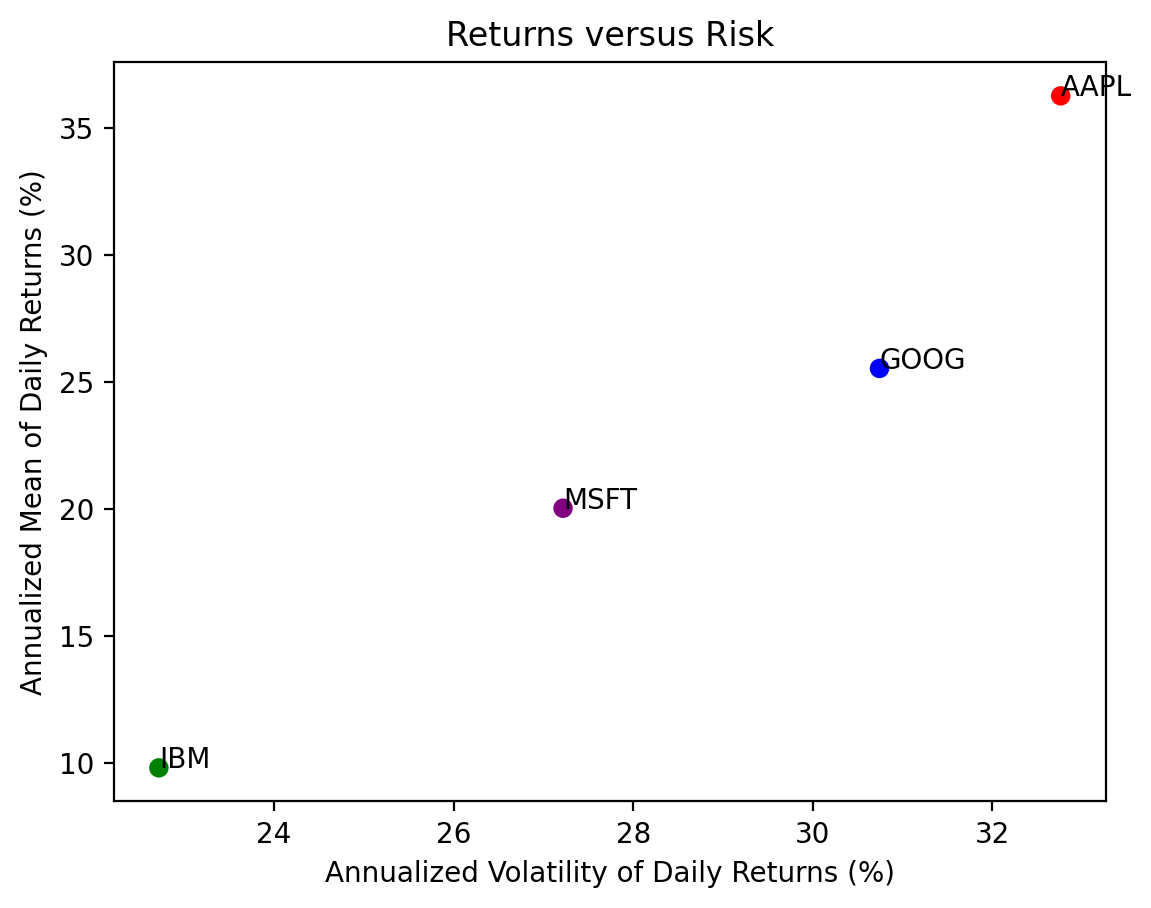
\includegraphics{mckinney_05_practice_02_files/figure-pdf/cell-21-output-1.png}

}

\end{figure}

\hypertarget{repeat-the-previous-calculations-and-plot-for-the-stocks-in-the-dow-jones-industrial-index-djia}{%
\subsection{Repeat the previous calculations and plot for the stocks in
the Dow-Jones Industrial Index
(DJIA)}\label{repeat-the-previous-calculations-and-plot-for-the-stocks-in-the-dow-jones-industrial-index-djia}}

We can find the current DJIA stocks on
\href{https://en.wikipedia.org/wiki/Dow_Jones_Industrial_Average}{Wikipedia}.
We will need to download new data, into \texttt{tickers2},
\texttt{prices2}, and \texttt{returns2}.

\begin{Shaded}
\begin{Highlighting}[]
\NormalTok{url2 }\OperatorTok{=} \StringTok{\textquotesingle{}https://en.wikipedia.org/wiki/Dow\_Jones\_Industrial\_Average\textquotesingle{}}
\NormalTok{wiki2 }\OperatorTok{=}\NormalTok{ pd.read\_html(io}\OperatorTok{=}\NormalTok{url2)}
\NormalTok{tickers2 }\OperatorTok{=}\NormalTok{ wiki2[}\DecValTok{1}\NormalTok{][}\StringTok{\textquotesingle{}Symbol\textquotesingle{}}\NormalTok{].to\_list()}
\NormalTok{tickers2[:}\DecValTok{5}\NormalTok{]}
\end{Highlighting}
\end{Shaded}

\begin{verbatim}
['MMM', 'AXP', 'AMGN', 'AAPL', 'BA']
\end{verbatim}

\begin{Shaded}
\begin{Highlighting}[]
\NormalTok{prices2 }\OperatorTok{=}\NormalTok{ yf.download(tickers}\OperatorTok{=}\NormalTok{tickers2)}
\end{Highlighting}
\end{Shaded}

\begin{verbatim}
[*********************100%%**********************]  30 of 30 completed
\end{verbatim}

\begin{Shaded}
\begin{Highlighting}[]
\NormalTok{returns2 }\OperatorTok{=}\NormalTok{ (}
\NormalTok{    prices2[}\StringTok{\textquotesingle{}Adj Close\textquotesingle{}}\NormalTok{] }\CommentTok{\# slice the adj close columns for all 30 tickers}
\NormalTok{    .iloc[:}\OperatorTok{{-}}\DecValTok{1}\NormalTok{] }\CommentTok{\# drop last row with incomplete prices because we are before the close}
\NormalTok{    .pct\_change() }\CommentTok{\# calculate returns}
\NormalTok{    .dropna() }\CommentTok{\# drops any row with incomplete data}
\NormalTok{)}

\NormalTok{returns2}
\end{Highlighting}
\end{Shaded}

\begin{longtable}[]{@{}llllllllllllllllllllll@{}}
\toprule\noalign{}
& AAPL & AMGN & AXP & BA & CAT & CRM & CSCO & CVX & DIS & DOW & ... &
MRK & MSFT & NKE & PG & TRV & UNH & V & VZ & WBA & WMT \\
Date & & & & & & & & & & & & & & & & & & & & & \\
\midrule\noalign{}
\endhead
\bottomrule\noalign{}
\endlastfoot
2019-03-21 & 0.0368 & 0.0040 & 0.0095 & -0.0092 & 0.0079 & 0.0210 &
0.0128 & 0.0094 & -0.0121 & -0.0165 & ... & 0.0106 & 0.0230 & 0.0152 &
0.0076 & 0.0231 & 0.0061 & 0.0133 & 0.0108 & 0.0129 & 0.0043 \\
2019-03-22 & -0.0207 & -0.0270 & -0.0211 & -0.0283 & -0.0320 & -0.0326 &
-0.0222 & -0.0220 & -0.0040 & -0.0078 & ... & -0.0080 & -0.0264 &
-0.0661 & -0.0081 & 0.0039 & -0.0196 & -0.0175 & 0.0252 & -0.0187 &
-0.0079 \\
2019-03-25 & -0.0121 & -0.0006 & -0.0038 & 0.0229 & 0.0124 & -0.0038 &
-0.0002 & -0.0016 & -0.0041 & 0.0113 & ... & 0.0007 & 0.0052 & 0.0017 &
0.0030 & 0.0004 & -0.0009 & -0.0003 & 0.0054 & -0.0115 & -0.0011 \\
2019-03-26 & -0.0103 & 0.0090 & 0.0042 & -0.0002 & 0.0035 & -0.0092 &
0.0095 & 0.0101 & 0.0218 & -0.0061 & ... & 0.0069 & 0.0021 & 0.0128 &
0.0104 & 0.0002 & -0.0141 & 0.0148 & 0.0092 & 0.0037 & 0.0015 \\
2019-03-27 & 0.0090 & -0.0104 & -0.0047 & 0.0103 & -0.0049 & -0.0269 &
-0.0017 & -0.0108 & 0.0013 & 0.0256 & ... & -0.0076 & -0.0097 & -0.0035
& -0.0012 & 0.0101 & -0.0069 & -0.0070 & 0.0041 & 0.0050 & -0.0113 \\
... & ... & ... & ... & ... & ... & ... & ... & ... & ... & ... & ... &
... & ... & ... & ... & ... & ... & ... & ... & ... & ... \\
2024-01-26 & -0.0090 & 0.0049 & 0.0710 & 0.0178 & -0.0045 & 0.0033 &
-0.0036 & 0.0038 & 0.0053 & -0.0160 & ... & 0.0057 & -0.0023 & 0.0196 &
0.0033 & -0.0004 & 0.0199 & -0.0171 & 0.0026 & -0.0113 & 0.0088 \\
2024-01-29 & -0.0036 & 0.0054 & -0.0028 & -0.0014 & 0.0128 & 0.0283 &
0.0029 & -0.0004 & 0.0223 & 0.0002 & ... & 0.0038 & 0.0143 & 0.0110 &
0.0001 & -0.0015 & 0.0027 & 0.0213 & -0.0083 & -0.0057 & 0.0047 \\
2024-01-30 & -0.0192 & 0.0037 & 0.0164 & -0.0231 & 0.0050 & -0.0005 &
-0.0010 & 0.0070 & -0.0056 & 0.0074 & ... & 0.0031 & -0.0028 & 0.0029 &
0.0085 & 0.0115 & -0.0018 & 0.0128 & 0.0100 & 0.0018 & 0.0033 \\
2024-01-31 & -0.0194 & -0.0011 & -0.0167 & 0.0529 & -0.0146 & -0.0231 &
-0.0394 & -0.0179 & -0.0092 & -0.0160 & ... & -0.0072 & -0.0269 &
-0.0254 & -0.0022 & -0.0102 & 0.0161 & -0.0140 & -0.0028 & -0.0083 &
-0.0021 \\
2024-02-01 & 0.0133 & 0.0328 & 0.0124 & -0.0058 & 0.0246 & 0.0096 &
0.0000 & 0.0031 & 0.0105 & -0.0011 & ... & 0.0464 & 0.0156 & 0.0023 &
0.0130 & 0.0031 & -0.0090 & 0.0139 & 0.0033 & 0.0301 & 0.0185 \\
\end{longtable}

\begin{Shaded}
\begin{Highlighting}[]
\NormalTok{vols2 }\OperatorTok{=}\NormalTok{ returns2.std().mul(np.sqrt(}\DecValTok{252}\NormalTok{) }\OperatorTok{*} \DecValTok{100}\NormalTok{)}
\NormalTok{means2 }\OperatorTok{=}\NormalTok{ returns2.mean().mul(}\DecValTok{252} \OperatorTok{*} \DecValTok{100}\NormalTok{)}

\NormalTok{plt.scatter(}
\NormalTok{    x}\OperatorTok{=}\NormalTok{vols2,}
\NormalTok{    y}\OperatorTok{=}\NormalTok{means2}
\NormalTok{)}

\NormalTok{plt.xlabel(}\StringTok{\textquotesingle{}Annualized Volatility of Daily Returns (\%)\textquotesingle{}}\NormalTok{)}
\NormalTok{plt.ylabel(}\StringTok{\textquotesingle{}Annualized Mean of Daily Returns (\%)\textquotesingle{}}\NormalTok{)}

\CommentTok{\# plt.xlim((0, vols2.max() + 5))}
\CommentTok{\# plt.ylim((0, means2.max() + 5))}

\CommentTok{\# add tickers to each point}
\ControlFlowTok{for}\NormalTok{ i }\KeywordTok{in}\NormalTok{ means2.index: }\CommentTok{\# loop over ticker index}
\NormalTok{    plt.text( }\CommentTok{\# plots string s at coordinates x and y}
\NormalTok{        x}\OperatorTok{=}\NormalTok{vols2[i], }\CommentTok{\# indexes volatility}
\NormalTok{        y}\OperatorTok{=}\NormalTok{means2[i], }\CommentTok{\# indexes mean return}
\NormalTok{        s}\OperatorTok{=}\NormalTok{i }\CommentTok{\# ticker index}
\NormalTok{    )}

\NormalTok{plt.title(}\StringTok{\textquotesingle{}Returns versus Risk\textquotesingle{}}\NormalTok{)}
\NormalTok{plt.show() }\CommentTok{\# suppresses output of last function call}
\end{Highlighting}
\end{Shaded}

\begin{figure}[H]

{\centering 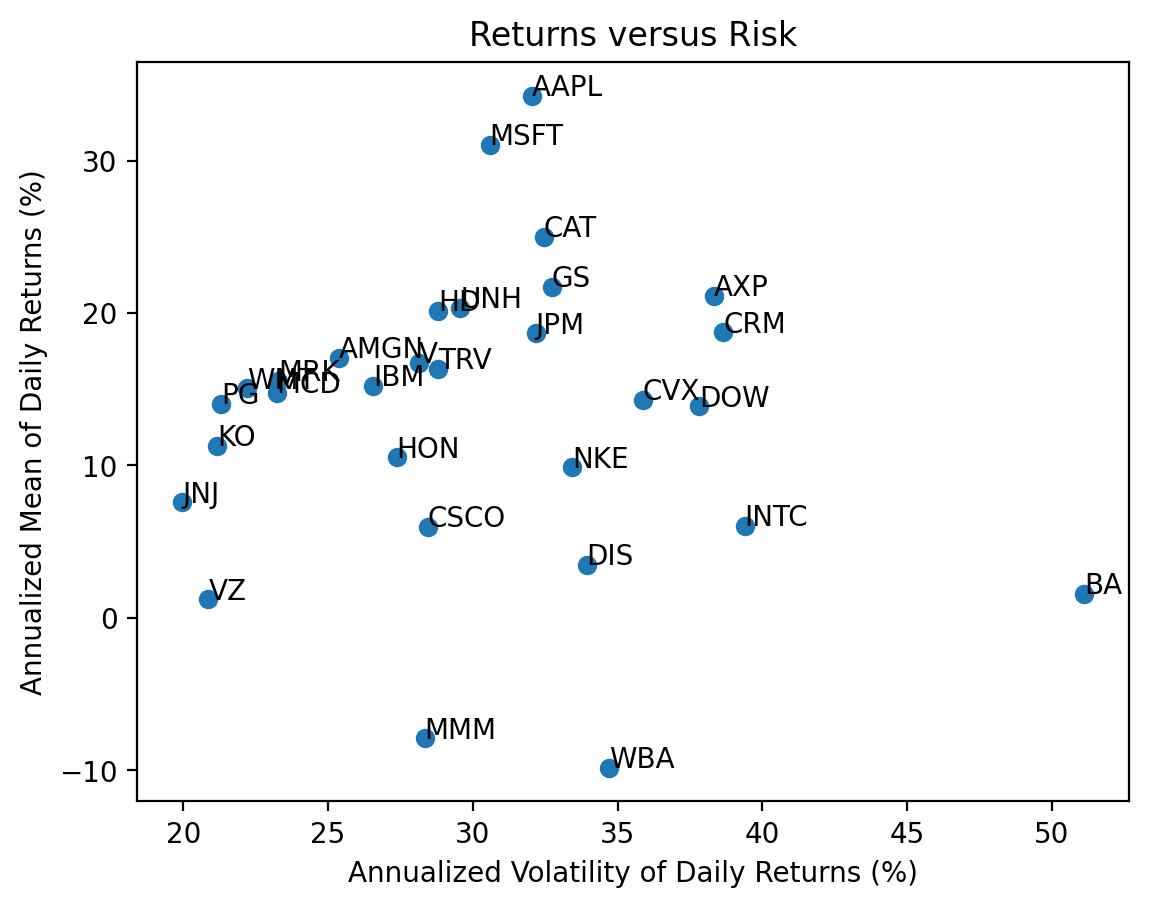
\includegraphics{mckinney_05_practice_02_files/figure-pdf/cell-25-output-1.png}

}

\end{figure}

With 30 stocks we see there is no relation between returns and
volatility because most volatility is \emph{diversifiable} and
uncompensated.

\hypertarget{calculate-total-returns-for-the-stocks-in-the-djia}{%
\subsection{Calculate total returns for the stocks in the
DJIA}\label{calculate-total-returns-for-the-stocks-in-the-djia}}

We can use the \texttt{.prod()} method to compound returns as
\(1 + R_T = \prod_{t=1}^T (1 + R_t)\). Technically, we should write
\(R_T\) as \(R_{0,T}\), but we typically omit the subscript \(0\).

I prefer to chain these operations, with \texttt{.add(1)}, then
\texttt{.prod()}, then \texttt{.sub(1)}.

\begin{Shaded}
\begin{Highlighting}[]
\NormalTok{total\_returns2 }\OperatorTok{=}\NormalTok{ returns2.add(}\DecValTok{1}\NormalTok{).prod().sub(}\DecValTok{1}\NormalTok{)}

\NormalTok{total\_returns2.iloc[:}\DecValTok{5}\NormalTok{]}
\end{Highlighting}
\end{Shaded}

\begin{verbatim}
AAPL    3.1210
AMGN    0.9635
AXP     0.9687
BA     -0.4289
CAT     1.6083
dtype: float64
\end{verbatim}

\hypertarget{plot-the-distribution-of-total-returns-for-the-stocks-in-the-djia}{%
\subsection{Plot the distribution of total returns for the stocks in the
DJIA}\label{plot-the-distribution-of-total-returns-for-the-stocks-in-the-djia}}

We can plot a histogram, using either the \texttt{plt.hist()} function
or the \texttt{.plot(kind=\textquotesingle{}hist\textquotesingle{})}
method.

A histogram is a great way to visualize data!

\begin{Shaded}
\begin{Highlighting}[]
\NormalTok{(}
\NormalTok{    returns2}
\NormalTok{    .add(}\DecValTok{1}\NormalTok{)}
\NormalTok{    .prod()}
\NormalTok{    .sub(}\DecValTok{1}\NormalTok{)}
\NormalTok{    .mul(}\DecValTok{100}\NormalTok{)}
\NormalTok{    .plot(kind}\OperatorTok{=}\StringTok{\textquotesingle{}hist\textquotesingle{}}\NormalTok{, bins}\OperatorTok{=}\DecValTok{20}\NormalTok{)}
\NormalTok{)}

\NormalTok{start\_date }\OperatorTok{=}\NormalTok{ returns2.index.}\BuiltInTok{min}\NormalTok{()}
\NormalTok{stop\_date }\OperatorTok{=}\NormalTok{ returns2.index.}\BuiltInTok{max}\NormalTok{()}

\NormalTok{plt.xlabel(}\StringTok{\textquotesingle{}Total Return (\%)\textquotesingle{}}\NormalTok{)}
\NormalTok{plt.title(}\SpecialStringTok{f\textquotesingle{}Distribution of Total Returns for DJIA Stocks}\CharTok{\textbackslash{}n}\SpecialStringTok{ from }\SpecialCharTok{\{}\NormalTok{start\_date}\SpecialCharTok{:}\OperatorTok{\%}\NormalTok{B }\OperatorTok{\%}\NormalTok{Y}\SpecialCharTok{\}}\SpecialStringTok{ through }\SpecialCharTok{\{}\NormalTok{stop\_date}\SpecialCharTok{:}\OperatorTok{\%}\NormalTok{B }\OperatorTok{\%}\NormalTok{Y}\SpecialCharTok{\}}\SpecialStringTok{\textquotesingle{}}\NormalTok{)}
\NormalTok{plt.show()}
\end{Highlighting}
\end{Shaded}

\begin{figure}[H]

{\centering 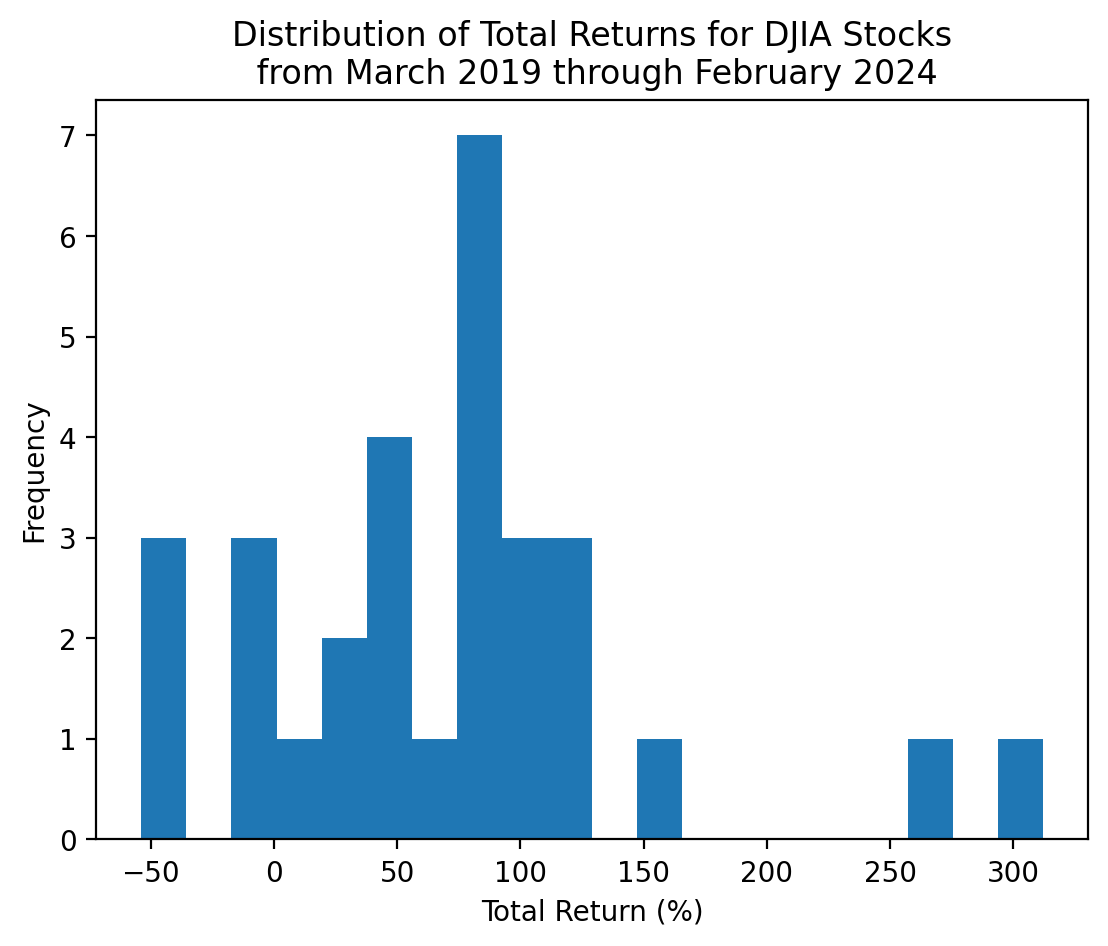
\includegraphics{mckinney_05_practice_02_files/figure-pdf/cell-27-output-1.png}

}

\end{figure}

With only 30 stocks, we can actually visualize each total return!

\begin{Shaded}
\begin{Highlighting}[]
\NormalTok{(}
\NormalTok{    returns2}
\NormalTok{    .add(}\DecValTok{1}\NormalTok{)}
\NormalTok{    .prod()}
\NormalTok{    .sub(}\DecValTok{1}\NormalTok{)}
\NormalTok{    .sort\_values() }\CommentTok{\# sort by total returns}
\NormalTok{    .mul(}\DecValTok{100}\NormalTok{)}
\NormalTok{    .plot(kind}\OperatorTok{=}\StringTok{\textquotesingle{}barh\textquotesingle{}}\NormalTok{) }\CommentTok{\# horizontal bar chart}
\NormalTok{)}

\NormalTok{start\_date }\OperatorTok{=}\NormalTok{ returns2.index.}\BuiltInTok{min}\NormalTok{()}
\NormalTok{stop\_date }\OperatorTok{=}\NormalTok{ returns2.index.}\BuiltInTok{max}\NormalTok{()}

\NormalTok{plt.xlabel(}\StringTok{\textquotesingle{}Total Return (\%)\textquotesingle{}}\NormalTok{)}
\NormalTok{plt.ylabel(}\StringTok{\textquotesingle{}Ticker\textquotesingle{}}\NormalTok{)}
\NormalTok{plt.title(}\SpecialStringTok{f\textquotesingle{}Distribution of Total Returns for DJIA Stocks}\CharTok{\textbackslash{}n}\SpecialStringTok{ from }\SpecialCharTok{\{}\NormalTok{start\_date}\SpecialCharTok{:}\OperatorTok{\%}\NormalTok{B }\OperatorTok{\%}\NormalTok{Y}\SpecialCharTok{\}}\SpecialStringTok{ through }\SpecialCharTok{\{}\NormalTok{stop\_date}\SpecialCharTok{:}\OperatorTok{\%}\NormalTok{B }\OperatorTok{\%}\NormalTok{Y}\SpecialCharTok{\}}\SpecialStringTok{\textquotesingle{}}\NormalTok{)}
\NormalTok{plt.show()}
\end{Highlighting}
\end{Shaded}

\begin{figure}[H]

{\centering 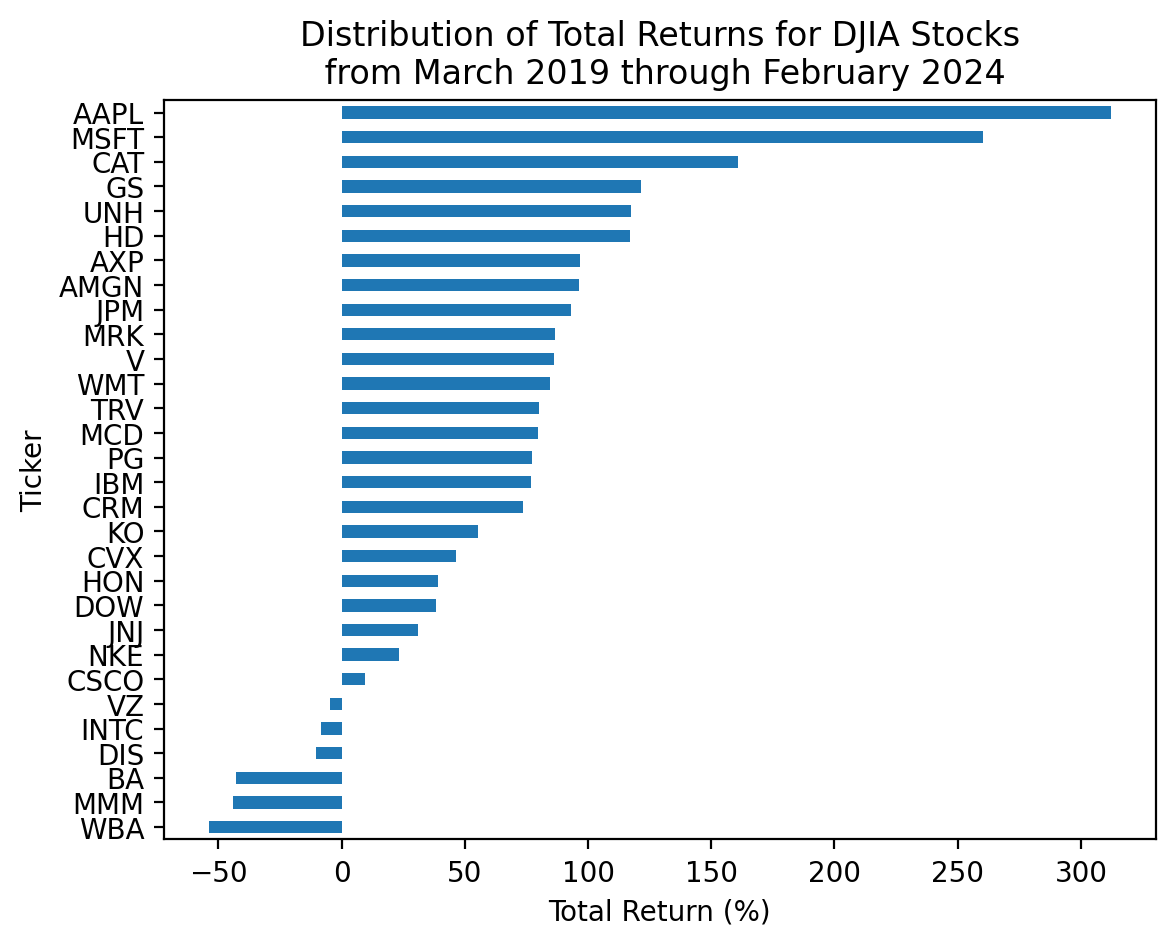
\includegraphics{mckinney_05_practice_02_files/figure-pdf/cell-28-output-1.png}

}

\end{figure}

\hypertarget{which-stocks-have-the-minimum-and-maximum-total-returns}{%
\subsection{Which stocks have the minimum and maximum total
returns?}\label{which-stocks-have-the-minimum-and-maximum-total-returns}}

If we want the \emph{values}, the \texttt{.min()} and \texttt{.max()}
methods are the way to go!

\begin{Shaded}
\begin{Highlighting}[]
\NormalTok{total\_returns2.}\BuiltInTok{min}\NormalTok{()}
\end{Highlighting}
\end{Shaded}

\begin{verbatim}
-0.5384
\end{verbatim}

\begin{Shaded}
\begin{Highlighting}[]
\NormalTok{total\_returns2.}\BuiltInTok{max}\NormalTok{()}
\end{Highlighting}
\end{Shaded}

\begin{verbatim}
3.1210
\end{verbatim}

If we want the \emph{ticker}, the \texttt{.idxmin()} and
\texttt{.idxmax()} methods are the way to go!

\begin{Shaded}
\begin{Highlighting}[]
\NormalTok{total\_returns2.idxmin()}
\end{Highlighting}
\end{Shaded}

\begin{verbatim}
'WBA'
\end{verbatim}

\begin{Shaded}
\begin{Highlighting}[]
\NormalTok{total\_returns2.idxmax()}
\end{Highlighting}
\end{Shaded}

\begin{verbatim}
'AAPL'
\end{verbatim}

If we want the smallest and the largest together, we can chain a few
methods!

\begin{Shaded}
\begin{Highlighting}[]
\NormalTok{total\_returns2.sort\_values().iloc[[}\DecValTok{0}\NormalTok{, }\OperatorTok{{-}}\DecValTok{1}\NormalTok{]]}
\end{Highlighting}
\end{Shaded}

\begin{verbatim}
WBA    -0.5384
AAPL    3.1210
dtype: float64
\end{verbatim}

Not the exactly right tool here, but the
\texttt{.nsmallest()\textquotesingle{}\ and}.nlargest()` methods are
really useful!

\begin{Shaded}
\begin{Highlighting}[]
\NormalTok{total\_returns2.nsmallest(}\DecValTok{3}\NormalTok{)}
\end{Highlighting}
\end{Shaded}

\begin{verbatim}
WBA   -0.5384
MMM   -0.4408
BA    -0.4289
dtype: float64
\end{verbatim}

\begin{Shaded}
\begin{Highlighting}[]
\NormalTok{total\_returns2.nlargest(}\DecValTok{3}\NormalTok{)}
\end{Highlighting}
\end{Shaded}

\begin{verbatim}
AAPL   3.1210
MSFT   2.6028
CAT    1.6083
dtype: float64
\end{verbatim}

\hypertarget{plot-the-cumulative-returns-for-the-stocks-in-the-djia}{%
\subsection{Plot the cumulative returns for the stocks in the
DJIA}\label{plot-the-cumulative-returns-for-the-stocks-in-the-djia}}

We can use the cumulative product method \texttt{.cumprod()} to
calculate the right hand side of the formula above.

\begin{Shaded}
\begin{Highlighting}[]
\NormalTok{(}
\NormalTok{    returns2}
\NormalTok{    .add(}\DecValTok{1}\NormalTok{)}
\NormalTok{    .cumprod()}
\NormalTok{    .sub(}\DecValTok{1}\NormalTok{)}
\NormalTok{    .mul(}\DecValTok{100}\NormalTok{)}
\NormalTok{    .plot(legend}\OperatorTok{=}\VariableTok{False}\NormalTok{, linewidth}\OperatorTok{=}\FloatTok{0.5}\NormalTok{) }\CommentTok{\# with 30 stocks, this legend is too big to be useful}
\NormalTok{)}
\NormalTok{start\_date }\OperatorTok{=}\NormalTok{ returns2.index.}\BuiltInTok{min}\NormalTok{()}
\NormalTok{stop\_date }\OperatorTok{=}\NormalTok{ returns2.index.}\BuiltInTok{max}\NormalTok{()}

\NormalTok{plt.ylabel(}\StringTok{\textquotesingle{}Cumulative Return (\%)\textquotesingle{}}\NormalTok{)}
\NormalTok{plt.title(}\SpecialStringTok{f\textquotesingle{}Cumulative Returns for DJIA Stocks}\CharTok{\textbackslash{}n}\SpecialStringTok{ from }\SpecialCharTok{\{}\NormalTok{start\_date}\SpecialCharTok{:}\OperatorTok{\%}\NormalTok{B }\OperatorTok{\%}\NormalTok{Y}\SpecialCharTok{\}}\SpecialStringTok{ through }\SpecialCharTok{\{}\NormalTok{stop\_date}\SpecialCharTok{:}\OperatorTok{\%}\NormalTok{B }\OperatorTok{\%}\NormalTok{Y}\SpecialCharTok{\}}\SpecialStringTok{\textquotesingle{}}\NormalTok{)}
\NormalTok{plt.show()}
\end{Highlighting}
\end{Shaded}

\begin{figure}[H]

{\centering 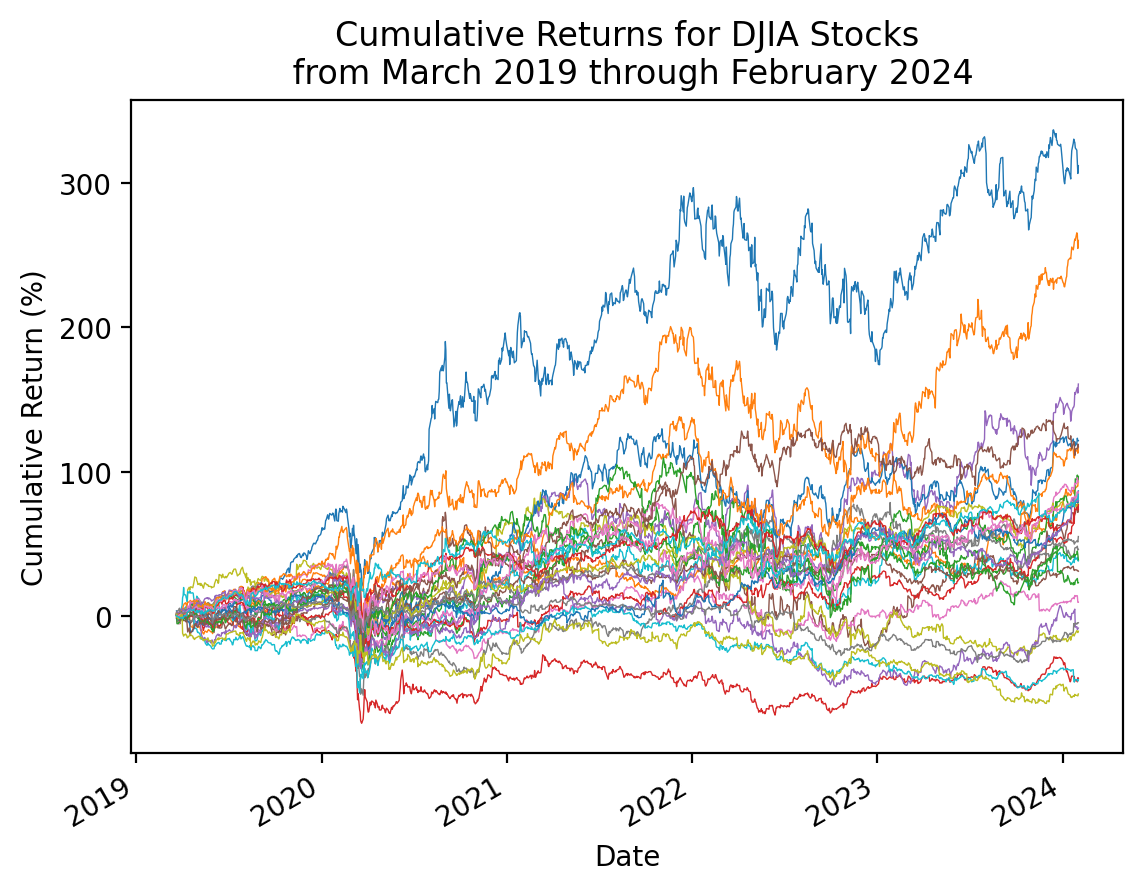
\includegraphics{mckinney_05_practice_02_files/figure-pdf/cell-36-output-1.png}

}

\end{figure}

\hypertarget{repeat-the-plot-above-with-only-the-minimum-and-maximum-total-returns}{%
\subsection{Repeat the plot above with only the minimum and maximum
total
returns}\label{repeat-the-plot-above-with-only-the-minimum-and-maximum-total-returns}}

\begin{Shaded}
\begin{Highlighting}[]
\NormalTok{total\_returns2.sort\_values().iloc[[}\DecValTok{0}\NormalTok{, }\OperatorTok{{-}}\DecValTok{1}\NormalTok{]].index}
\end{Highlighting}
\end{Shaded}

\begin{verbatim}
Index(['WBA', 'AAPL'], dtype='object')
\end{verbatim}

\begin{Shaded}
\begin{Highlighting}[]
\NormalTok{(}
\NormalTok{    returns2 }\CommentTok{\# all returns for all stocks}
\NormalTok{    [total\_returns2.sort\_values().iloc[[}\DecValTok{0}\NormalTok{, }\OperatorTok{{-}}\DecValTok{1}\NormalTok{]].index] }\CommentTok{\# slice min and max total return stocks}
\NormalTok{    .add(}\DecValTok{1}\NormalTok{)}
\NormalTok{    .cumprod()}
\NormalTok{    .sub(}\DecValTok{1}\NormalTok{)}
\NormalTok{    .mul(}\DecValTok{100}\NormalTok{)}
\NormalTok{    .plot()}
\NormalTok{)}
\NormalTok{start\_date }\OperatorTok{=}\NormalTok{ returns2.index.}\BuiltInTok{min}\NormalTok{()}
\NormalTok{stop\_date }\OperatorTok{=}\NormalTok{ returns2.index.}\BuiltInTok{max}\NormalTok{()}

\NormalTok{plt.ylabel(}\StringTok{\textquotesingle{}Cumulative Return (\%)\textquotesingle{}}\NormalTok{)}
\NormalTok{plt.title(}\SpecialStringTok{f\textquotesingle{}Cumulative Returns for DJIA Stocks}\CharTok{\textbackslash{}n}\SpecialStringTok{ from }\SpecialCharTok{\{}\NormalTok{start\_date}\SpecialCharTok{:}\OperatorTok{\%}\NormalTok{B }\OperatorTok{\%}\NormalTok{Y}\SpecialCharTok{\}}\SpecialStringTok{ through }\SpecialCharTok{\{}\NormalTok{stop\_date}\SpecialCharTok{:}\OperatorTok{\%}\NormalTok{B }\OperatorTok{\%}\NormalTok{Y}\SpecialCharTok{\}}\SpecialStringTok{\textquotesingle{}}\NormalTok{)}
\NormalTok{plt.show()}
\end{Highlighting}
\end{Shaded}

\begin{figure}[H]

{\centering 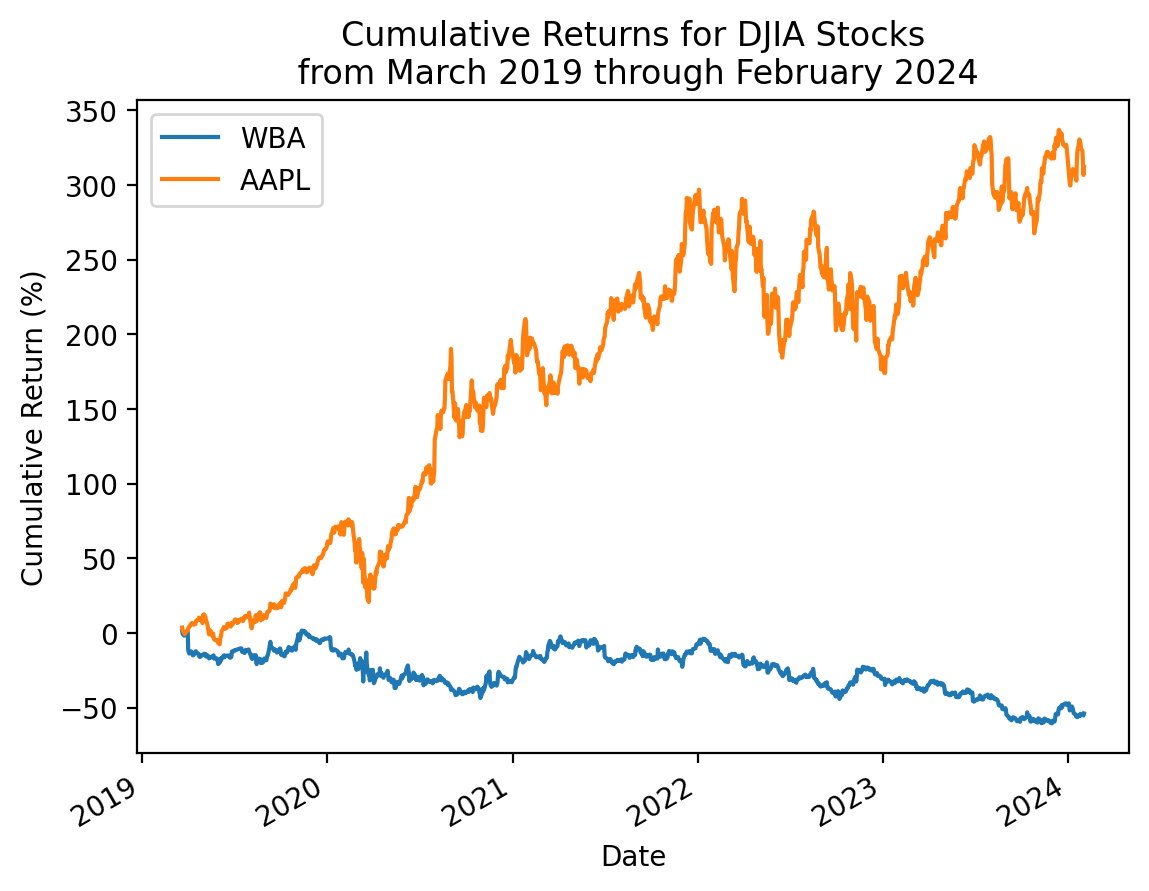
\includegraphics{mckinney_05_practice_02_files/figure-pdf/cell-38-output-1.png}

}

\end{figure}

\hypertarget{mckinney-chapter-5---practice-for-section-03}{%
\chapter{McKinney Chapter 5 - Practice for Section
03}\label{mckinney-chapter-5---practice-for-section-03}}

\hypertarget{announcements-13}{%
\section{Announcements}\label{announcements-13}}

\begin{enumerate}
\def\labelenumi{\arabic{enumi}.}
\tightlist
\item
  No DataCamp this week, but I suggest you keep working on it
\item
  Keep forming groups, and I will post our first project early next week
\end{enumerate}

\hypertarget{minute-recap-12}\NormalTok{precision }\DecValTok{4}
\NormalTok{pd.options.display.float\_format }\OperatorTok{=} \StringTok{\textquotesingle{}}\SpecialCharTok{\{:.4f\}}\StringTok{\textquotesingle{}}\NormalTok{.}\BuiltInTok{format}
\OperatorTok{\%}\NormalTok{config InlineBackend.figure\_format }\OperatorTok{=} \StringTok{\textquotesingle{}retina\textquotesingle{}}
\end{Highlighting}
\end{Shaded}

pandas provides two \emph{very useful} data structures:

\begin{enumerate}
\def\labelenumi{\arabic{enumi}.}
\tightlist
\item
  Data frames are like a worksheet in an Excel workbook (2-D, mixed data
  type)
\item
  Series are like a column in a worksheet in an Excel workbook (1-D, one
  data type)
\end{enumerate}

\begin{Shaded}
\begin{Highlighting}[]
\NormalTok{np.random.seed(}\DecValTok{42}\NormalTok{)}
\NormalTok{df }\OperatorTok{=}\NormalTok{ pd.DataFrame(}
\NormalTok{    data}\OperatorTok{=}\NormalTok{np.random.randn(}\DecValTok{4}\NormalTok{, }\DecValTok{4}\NormalTok{),}
\NormalTok{    index}\OperatorTok{=}\BuiltInTok{list}\NormalTok{(}\StringTok{\textquotesingle{}ABCD\textquotesingle{}}\NormalTok{),}
\NormalTok{    columns}\OperatorTok{=}\BuiltInTok{list}\NormalTok{(}\StringTok{\textquotesingle{}abcd\textquotesingle{}}\NormalTok{)}
\NormalTok{)}

\NormalTok{df}
\end{Highlighting}
\end{Shaded}

\begin{longtable}[]{@{}lllll@{}}
\toprule\noalign{}
& a & b & c & d \\
\midrule\noalign{}
\endhead
\bottomrule\noalign{}
\endlastfoot
A & 0.4967 & -0.1383 & 0.6477 & 1.5230 \\
B & -0.2342 & -0.2341 & 1.5792 & 0.7674 \\
C & -0.4695 & 0.5426 & -0.4634 & -0.4657 \\
D & 0.2420 & -1.9133 & -1.7249 & -0.5623 \\
\end{longtable}

How can we slice the first two rows and three columns? We can slice data
frames two ways:

\begin{enumerate}
\def\labelenumi{\arabic{enumi}.}
\tightlist
\item
  Using integer locations and the \texttt{.iloc{[}{]}} method
\item
  Using row and column names with the \texttt{.loc{[}{]}} method
\end{enumerate}

\begin{Shaded}
\begin{Highlighting}[]
\NormalTok{df.iloc[:}\DecValTok{2}\NormalTok{, :}\DecValTok{3}\NormalTok{] }\CommentTok{\# slice with j,k notation, like NumPy}
\end{Highlighting}
\end{Shaded}

\begin{longtable}[]{@{}llll@{}}
\toprule\noalign{}
& a & b & c \\
\midrule\noalign{}
\endhead
\bottomrule\noalign{}
\endlastfoot
A & 0.4967 & -0.1383 & 0.6477 \\
B & -0.2342 & -0.2341 & 1.5792 \\
\end{longtable}

\textbf{\emph{When we slice by names or labels, we get both left and
right edges included!}}

\begin{Shaded}
\begin{Highlighting}[]
\NormalTok{df.loc[}\StringTok{\textquotesingle{}A\textquotesingle{}}\NormalTok{:}\StringTok{\textquotesingle{}B\textquotesingle{}}\NormalTok{, }\StringTok{\textquotesingle{}a\textquotesingle{}}\NormalTok{:}\StringTok{\textquotesingle{}c\textquotesingle{}}\NormalTok{]}
\end{Highlighting}
\end{Shaded}

\begin{longtable}[]{@{}llll@{}}
\toprule\noalign{}
& a & b & c \\
\midrule\noalign{}
\endhead
\bottomrule\noalign{}
\endlastfoot
A & 0.4967 & -0.1383 & 0.6477 \\
B & -0.2342 & -0.2341 & 1.5792 \\
\end{longtable}

We can easily add columns!

\begin{Shaded}
\begin{Highlighting}[]
\NormalTok{df[}\StringTok{\textquotesingle{}e\textquotesingle{}}\NormalTok{] }\OperatorTok{=} \DecValTok{5} \CommentTok{\# broadcasts to every row in df}

\NormalTok{df}
\end{Highlighting}
\end{Shaded}

\begin{longtable}[]{@{}llllll@{}}
\toprule\noalign{}
& a & b & c & d & e \\
\midrule\noalign{}
\endhead
\bottomrule\noalign{}
\endlastfoot
A & 0.4967 & -0.1383 & 0.6477 & 1.5230 & 5 \\
B & -0.2342 & -0.2341 & 1.5792 & 0.7674 & 5 \\
C & -0.4695 & 0.5426 & -0.4634 & -0.4657 & 5 \\
D & 0.2420 & -1.9133 & -1.7249 & -0.5623 & 5 \\
\end{longtable}

\begin{Shaded}
\begin{Highlighting}[]
\NormalTok{df[}\StringTok{\textquotesingle{}e\textquotesingle{}}\NormalTok{] }\OperatorTok{=}\NormalTok{ np.random.randn(}\DecValTok{4}\NormalTok{)}

\NormalTok{df}
\end{Highlighting}
\end{Shaded}

\begin{longtable}[]{@{}llllll@{}}
\toprule\noalign{}
& a & b & c & d & e \\
\midrule\noalign{}
\endhead
\bottomrule\noalign{}
\endlastfoot
A & 0.4967 & -0.1383 & 0.6477 & 1.5230 & -1.0128 \\
B & -0.2342 & -0.2341 & 1.5792 & 0.7674 & 0.3142 \\
C & -0.4695 & 0.5426 & -0.4634 & -0.4657 & -0.9080 \\
D & 0.2420 & -1.9133 & -1.7249 & -0.5623 & -1.4123 \\
\end{longtable}

A series is the other, 1-D data structure in pandas!

\begin{Shaded}
\begin{Highlighting}[]
\NormalTok{ser }\OperatorTok{=}\NormalTok{ pd.Series(data}\OperatorTok{=}\NormalTok{np.arange(}\FloatTok{2.}\NormalTok{), index}\OperatorTok{=}\NormalTok{[}\StringTok{\textquotesingle{}C\textquotesingle{}}\NormalTok{, }\StringTok{\textquotesingle{}D\textquotesingle{}}\NormalTok{]) }\CommentTok{\# the . in np.arange() makes the array floats}

\NormalTok{ser}
\end{Highlighting}
\end{Shaded}

\begin{verbatim}
C   0.0000
D   1.0000
dtype: float64
\end{verbatim}

\begin{Shaded}
\begin{Highlighting}[]
\NormalTok{df[}\StringTok{\textquotesingle{}f\textquotesingle{}}\NormalTok{] }\OperatorTok{=}\NormalTok{ ser}

\NormalTok{df}
\end{Highlighting}
\end{Shaded}

\begin{longtable}[]{@{}lllllll@{}}
\toprule\noalign{}
& a & b & c & d & e & f \\
\midrule\noalign{}
\endhead
\bottomrule\noalign{}
\endlastfoot
A & 0.4967 & -0.1383 & 0.6477 & 1.5230 & -1.0128 & NaN \\
B & -0.2342 & -0.2341 & 1.5792 & 0.7674 & 0.3142 & NaN \\
C & -0.4695 & 0.5426 & -0.4634 & -0.4657 & -0.9080 & 0.0000 \\
D & 0.2420 & -1.9133 & -1.7249 & -0.5623 & -1.4123 & 1.0000 \\
\end{longtable}

\hypertarget{practice-13}{%
\section{Practice}\label{practice-13}}

\begin{Shaded}
\begin{Highlighting}[]
\NormalTok{tickers }\OperatorTok{=} \StringTok{\textquotesingle{}AAPL IBM MSFT GOOG\textquotesingle{}}
\NormalTok{prices }\OperatorTok{=}\NormalTok{ yf.download(tickers}\OperatorTok{=}\NormalTok{tickers)}
\end{Highlighting}
\end{Shaded}

\begin{verbatim}
[*********************100%%**********************]  4 of 4 completed
\end{verbatim}

\begin{Shaded}
\begin{Highlighting}[]
\NormalTok{returns }\OperatorTok{=}\NormalTok{ (}
\NormalTok{    prices[}\StringTok{\textquotesingle{}Adj Close\textquotesingle{}}\NormalTok{] }\CommentTok{\# slice adj close column}
\NormalTok{    .iloc[:}\OperatorTok{{-}}\DecValTok{1}\NormalTok{] }\CommentTok{\# drop last row with intra day prices, which are sometimes missing}
\NormalTok{    .pct\_change() }\CommentTok{\# calculate returns}
\NormalTok{    .dropna() }\CommentTok{\# drop leading rows with at least one missing value}
\NormalTok{)}

\NormalTok{returns}
\end{Highlighting}
\end{Shaded}

\begin{longtable}[]{@{}lllll@{}}
\toprule\noalign{}
& AAPL & GOOG & IBM & MSFT \\
Date & & & & \\
\midrule\noalign{}
\endhead
\bottomrule\noalign{}
\endlastfoot
2004-08-20 & 0.0029 & 0.0794 & 0.0042 & 0.0030 \\
2004-08-23 & 0.0091 & 0.0101 & -0.0070 & 0.0044 \\
2004-08-24 & 0.0280 & -0.0414 & 0.0007 & 0.0000 \\
2004-08-25 & 0.0344 & 0.0108 & 0.0042 & 0.0114 \\
2004-08-26 & 0.0487 & 0.0180 & -0.0045 & -0.0040 \\
... & ... & ... & ... & ... \\
2024-01-26 & -0.0090 & 0.0010 & -0.0158 & -0.0023 \\
2024-01-29 & -0.0036 & 0.0068 & -0.0015 & 0.0143 \\
2024-01-30 & -0.0192 & -0.0116 & 0.0039 & -0.0028 \\
2024-01-31 & -0.0194 & -0.0735 & -0.0224 & -0.0269 \\
2024-02-01 & 0.0133 & 0.0064 & 0.0176 & 0.0156 \\
\end{longtable}

\hypertarget{what-are-the-mean-daily-returns-for-these-four-stocks-1}{%
\subsection{What are the mean daily returns for these four
stocks?}\label{what-are-the-mean-daily-returns-for-these-four-stocks-1}}

\begin{Shaded}
\begin{Highlighting}[]
\NormalTok{returns.mean() }\CommentTok{\# default axis=0 takes the mean of each column}
\end{Highlighting}
\end{Shaded}

\begin{verbatim}
AAPL   0.0014
GOOG   0.0010
IBM    0.0004
MSFT   0.0008
dtype: float64
\end{verbatim}

If we pass \texttt{axis=1}, we get the mean return on each day. We can
this an ``equally-weighted portfolio return.''
\[r_{p,t} = \sum_{i=0}^4 \frac{1}{4} r_{i, t}\]

\begin{Shaded}
\begin{Highlighting}[]
\NormalTok{returns.mean(axis}\OperatorTok{=}\DecValTok{1}\NormalTok{)}
\end{Highlighting}
\end{Shaded}

\begin{verbatim}
Date
2004-08-20    0.0224
2004-08-23    0.0041
2004-08-24   -0.0032
2004-08-25    0.0152
2004-08-26    0.0146
               ...  
2024-01-26   -0.0065
2024-01-29    0.0040
2024-01-30   -0.0074
2024-01-31   -0.0356
2024-02-01    0.0132
Length: 4896, dtype: float64
\end{verbatim}

\hypertarget{what-are-the-standard-deviations-of-daily-returns-for-these-four-stocks-1}{%
\subsection{What are the standard deviations of daily returns for these
four
stocks?}\label{what-are-the-standard-deviations-of-daily-returns-for-these-four-stocks-1}}

pandas calcualates sample statistics by default.

\begin{Shaded}
\begin{Highlighting}[]
\NormalTok{returns.std()}
\end{Highlighting}
\end{Shaded}

\begin{verbatim}
AAPL   0.0206
GOOG   0.0194
IBM    0.0143
MSFT   0.0171
dtype: float64
\end{verbatim}

\hypertarget{what-are-the-annualized-means-and-standard-deviations-of-daily-returns-for-these-four-stocks-1}{%
\subsection{\texorpdfstring{What are the \emph{annualized} means and
standard deviations of daily returns for these four
stocks?}{What are the annualized means and standard deviations of daily returns for these four stocks?}}\label{what-are-the-annualized-means-and-standard-deviations-of-daily-returns-for-these-four-stocks-1}}

We annualize mean returns by multiplying by \(T\) (\(T=252\) for daily
returns, \(T=12\) for month returns, and so on). We annualize standard
deviations by multiplying by \(\sqrt(T)\).

\begin{Shaded}
\begin{Highlighting}[]
\NormalTok{returns.mean().mul(}\DecValTok{252}\NormalTok{)}
\end{Highlighting}
\end{Shaded}

\begin{verbatim}
AAPL   0.3625
GOOG   0.2552
IBM    0.0980
MSFT   0.2002
dtype: float64
\end{verbatim}

\begin{Shaded}
\begin{Highlighting}[]
\NormalTok{returns.std().mul(np.sqrt(}\DecValTok{252}\NormalTok{))}
\end{Highlighting}
\end{Shaded}

\begin{verbatim}
AAPL   0.3276
GOOG   0.3074
IBM    0.2272
MSFT   0.2722
dtype: float64
\end{verbatim}

\hypertarget{plot-annualized-means-versus-standard-deviations-of-daily-returns-for-these-four-stocks-1}{%
\subsection{\texorpdfstring{Plot \emph{annualized} means versus standard
deviations of daily returns for these four
stocks}{Plot annualized means versus standard deviations of daily returns for these four stocks}}\label{plot-annualized-means-versus-standard-deviations-of-daily-returns-for-these-four-stocks-1}}

Use \texttt{plt.scatter()}, which expects arguments as \texttt{x}
(standard deviations) then \texttt{y} (means).

\begin{Shaded}
\begin{Highlighting}[]
\NormalTok{vols }\OperatorTok{=}\NormalTok{ returns.std().mul(np.sqrt(}\DecValTok{252}\NormalTok{) }\OperatorTok{*} \DecValTok{100}\NormalTok{)}
\NormalTok{means }\OperatorTok{=}\NormalTok{ returns.mean().mul(}\DecValTok{252} \OperatorTok{*} \DecValTok{100}\NormalTok{)}

\NormalTok{plt.scatter(}
\NormalTok{    x}\OperatorTok{=}\NormalTok{vols,}
\NormalTok{    y}\OperatorTok{=}\NormalTok{means}
\NormalTok{)}

\CommentTok{\# add tickers to each point}
\ControlFlowTok{for}\NormalTok{ i }\KeywordTok{in}\NormalTok{ means.index: }\CommentTok{\# loop over ticker index}
\NormalTok{    plt.text( }\CommentTok{\# plots string s at coordinates x and y}
\NormalTok{        x}\OperatorTok{=}\NormalTok{vols[i], }\CommentTok{\# indexes volatility}
\NormalTok{        y}\OperatorTok{=}\NormalTok{means[i], }\CommentTok{\# indexes mean return}
\NormalTok{        s}\OperatorTok{=}\NormalTok{i }\CommentTok{\# ticker index}
\NormalTok{    )}

\NormalTok{plt.xlabel(}\StringTok{\textquotesingle{}Annualized Volatility of Daily Returns (\%)\textquotesingle{}}\NormalTok{)}
\NormalTok{plt.ylabel(}\StringTok{\textquotesingle{}Annualized Mean of Daily Returns (\%)\textquotesingle{}}\NormalTok{)}

\NormalTok{plt.title(}\StringTok{\textquotesingle{}Returns versus Risk\textquotesingle{}}\NormalTok{)}
\NormalTok{plt.show()}
\end{Highlighting}
\end{Shaded}

\begin{figure}[H]

{\centering \includegraphics{mckinney_05_practice_03_files/figure-pdf/cell-18-output-1.png}

}

\end{figure}

\hypertarget{repeat-the-previous-calculations-and-plot-for-the-stocks-in-the-dow-jones-industrial-index-djia-1}{%
\subsection{Repeat the previous calculations and plot for the stocks in
the Dow-Jones Industrial Index
(DJIA)}\label{repeat-the-previous-calculations-and-plot-for-the-stocks-in-the-dow-jones-industrial-index-djia-1}}

We can find the current DJIA stocks on
\href{https://en.wikipedia.org/wiki/Dow_Jones_Industrial_Average}{Wikipedia}.
We will need to download new data, into \texttt{tickers2},
\texttt{prices2}, and \texttt{returns2}.

\begin{Shaded}
\begin{Highlighting}[]
\NormalTok{url2 }\OperatorTok{=} \StringTok{\textquotesingle{}https://en.wikipedia.org/wiki/Dow\_Jones\_Industrial\_Average\textquotesingle{}}
\NormalTok{wiki2 }\OperatorTok{=}\NormalTok{ pd.read\_html(io}\OperatorTok{=}\NormalTok{url2)}
\NormalTok{tickers2 }\OperatorTok{=}\NormalTok{ wiki2[}\DecValTok{1}\NormalTok{][}\StringTok{\textquotesingle{}Symbol\textquotesingle{}}\NormalTok{].to\_list()}
\NormalTok{tickers2[:}\DecValTok{5}\NormalTok{]}
\end{Highlighting}
\end{Shaded}

\begin{verbatim}
['MMM', 'AXP', 'AMGN', 'AAPL', 'BA']
\end{verbatim}

\begin{Shaded}
\begin{Highlighting}[]
\NormalTok{prices2 }\OperatorTok{=}\NormalTok{ yf.download(tickers}\OperatorTok{=}\NormalTok{tickers2)}
\end{Highlighting}
\end{Shaded}

\begin{verbatim}
[*********************100%%**********************]  30 of 30 completed
\end{verbatim}

\begin{Shaded}
\begin{Highlighting}[]
\NormalTok{returns2 }\OperatorTok{=}\NormalTok{ (}
\NormalTok{    prices2[}\StringTok{\textquotesingle{}Adj Close\textquotesingle{}}\NormalTok{] }\CommentTok{\# slide adj close for all stocks}
\NormalTok{    .iloc[:}\OperatorTok{{-}}\DecValTok{1}\NormalTok{] }\CommentTok{\# drop last day of adj close, which are intraday values before 4 PM}
\NormalTok{    .pct\_change() }\CommentTok{\# calculate returns}
\NormalTok{    .dropna() }\CommentTok{\# drop any dates with incomplete data}
\NormalTok{)}

\NormalTok{returns2}
\end{Highlighting}
\end{Shaded}

\begin{longtable}[]{@{}llllllllllllllllllllll@{}}
\toprule\noalign{}
& AAPL & AMGN & AXP & BA & CAT & CRM & CSCO & CVX & DIS & DOW & ... &
MRK & MSFT & NKE & PG & TRV & UNH & V & VZ & WBA & WMT \\
Date & & & & & & & & & & & & & & & & & & & & & \\
\midrule\noalign{}
\endhead
\bottomrule\noalign{}
\endlastfoot
2019-03-21 & 0.0368 & 0.0040 & 0.0095 & -0.0092 & 0.0079 & 0.0210 &
0.0128 & 0.0094 & -0.0121 & -0.0165 & ... & 0.0106 & 0.0230 & 0.0152 &
0.0076 & 0.0231 & 0.0061 & 0.0133 & 0.0108 & 0.0129 & 0.0043 \\
2019-03-22 & -0.0207 & -0.0270 & -0.0211 & -0.0283 & -0.0320 & -0.0326 &
-0.0222 & -0.0220 & -0.0040 & -0.0078 & ... & -0.0080 & -0.0264 &
-0.0661 & -0.0081 & 0.0039 & -0.0196 & -0.0175 & 0.0252 & -0.0187 &
-0.0079 \\
2019-03-25 & -0.0121 & -0.0006 & -0.0038 & 0.0229 & 0.0124 & -0.0038 &
-0.0002 & -0.0016 & -0.0041 & 0.0113 & ... & 0.0007 & 0.0052 & 0.0017 &
0.0030 & 0.0004 & -0.0009 & -0.0003 & 0.0054 & -0.0115 & -0.0011 \\
2019-03-26 & -0.0103 & 0.0090 & 0.0042 & -0.0002 & 0.0035 & -0.0092 &
0.0095 & 0.0101 & 0.0218 & -0.0061 & ... & 0.0069 & 0.0021 & 0.0128 &
0.0104 & 0.0002 & -0.0141 & 0.0148 & 0.0092 & 0.0037 & 0.0015 \\
2019-03-27 & 0.0090 & -0.0104 & -0.0047 & 0.0103 & -0.0049 & -0.0269 &
-0.0017 & -0.0108 & 0.0013 & 0.0256 & ... & -0.0076 & -0.0097 & -0.0035
& -0.0012 & 0.0102 & -0.0069 & -0.0070 & 0.0041 & 0.0050 & -0.0113 \\
... & ... & ... & ... & ... & ... & ... & ... & ... & ... & ... & ... &
... & ... & ... & ... & ... & ... & ... & ... & ... & ... \\
2024-01-26 & -0.0090 & 0.0049 & 0.0710 & 0.0178 & -0.0045 & 0.0033 &
-0.0036 & 0.0038 & 0.0053 & -0.0160 & ... & 0.0057 & -0.0023 & 0.0196 &
0.0033 & -0.0004 & 0.0199 & -0.0171 & 0.0026 & -0.0113 & 0.0088 \\
2024-01-29 & -0.0036 & 0.0054 & -0.0028 & -0.0014 & 0.0128 & 0.0283 &
0.0029 & -0.0004 & 0.0223 & 0.0002 & ... & 0.0038 & 0.0143 & 0.0110 &
0.0001 & -0.0015 & 0.0027 & 0.0213 & -0.0083 & -0.0057 & 0.0047 \\
2024-01-30 & -0.0192 & 0.0037 & 0.0164 & -0.0231 & 0.0050 & -0.0005 &
-0.0010 & 0.0070 & -0.0056 & 0.0074 & ... & 0.0031 & -0.0028 & 0.0029 &
0.0085 & 0.0115 & -0.0018 & 0.0128 & 0.0100 & 0.0018 & 0.0033 \\
2024-01-31 & -0.0194 & -0.0011 & -0.0167 & 0.0529 & -0.0146 & -0.0231 &
-0.0394 & -0.0179 & -0.0092 & -0.0160 & ... & -0.0072 & -0.0269 &
-0.0254 & -0.0022 & -0.0102 & 0.0161 & -0.0140 & -0.0028 & -0.0083 &
-0.0021 \\
2024-02-01 & 0.0133 & 0.0328 & 0.0124 & -0.0058 & 0.0246 & 0.0096 &
0.0000 & 0.0031 & 0.0105 & -0.0011 & ... & 0.0464 & 0.0156 & 0.0023 &
0.0130 & 0.0031 & -0.0090 & 0.0139 & 0.0033 & 0.0301 & 0.0185 \\
\end{longtable}

\begin{Shaded}
\begin{Highlighting}[]
\NormalTok{vols }\OperatorTok{=}\NormalTok{ returns2.std().mul(np.sqrt(}\DecValTok{252}\NormalTok{) }\OperatorTok{*} \DecValTok{100}\NormalTok{)}
\NormalTok{means }\OperatorTok{=}\NormalTok{ returns2.mean().mul(}\DecValTok{252} \OperatorTok{*} \DecValTok{100}\NormalTok{)}

\NormalTok{plt.scatter(}
\NormalTok{    x}\OperatorTok{=}\NormalTok{vols,}
\NormalTok{    y}\OperatorTok{=}\NormalTok{means}
\NormalTok{)}

\CommentTok{\# add tickers to each point}
\ControlFlowTok{for}\NormalTok{ i }\KeywordTok{in}\NormalTok{ means.index: }\CommentTok{\# loop over ticker index}
\NormalTok{    plt.text( }\CommentTok{\# plots string s at coordinates x and y}
\NormalTok{        x}\OperatorTok{=}\NormalTok{vols[i], }\CommentTok{\# indexes volatility}
\NormalTok{        y}\OperatorTok{=}\NormalTok{means[i], }\CommentTok{\# indexes mean return}
\NormalTok{        s}\OperatorTok{=}\NormalTok{i }\CommentTok{\# ticker index}
\NormalTok{    )}

\NormalTok{plt.xlabel(}\StringTok{\textquotesingle{}Annualized Volatility of Daily Returns (\%)\textquotesingle{}}\NormalTok{)}
\NormalTok{plt.ylabel(}\StringTok{\textquotesingle{}Annualized Mean of Daily Returns (\%)\textquotesingle{}}\NormalTok{)}

\NormalTok{plt.title(}\StringTok{\textquotesingle{}Returns versus Risk\textquotesingle{}}\NormalTok{)}
\NormalTok{plt.show()}
\end{Highlighting}
\end{Shaded}

\begin{figure}[H]

{\centering \includegraphics{mckinney_05_practice_03_files/figure-pdf/cell-22-output-1.png}

}

\end{figure}

\hypertarget{calculate-total-returns-for-the-stocks-in-the-djia-1}{%
\subsection{Calculate total returns for the stocks in the
DJIA}\label{calculate-total-returns-for-the-stocks-in-the-djia-1}}

We can use the \texttt{.prod()} method to compound returns as
\(1 + R_T = \prod_{t=1}^T (1 + R_t)\). Technically, we should write
\(R_T\) as \(R_{0,T}\), but we typically omit the subscript \(0\).

\begin{Shaded}
\begin{Highlighting}[]
\NormalTok{total\_returns2 }\OperatorTok{=}\NormalTok{ returns2.add(}\DecValTok{1}\NormalTok{).prod().sub(}\DecValTok{1}\NormalTok{)}

\NormalTok{total\_returns2.iloc[:}\DecValTok{5}\NormalTok{]}
\end{Highlighting}
\end{Shaded}

\begin{verbatim}
AAPL    3.1210
AMGN    0.9635
AXP     0.9687
BA     -0.4289
CAT     1.6083
dtype: float64
\end{verbatim}

\begin{Shaded}
\begin{Highlighting}[]
\NormalTok{np.allclose(((returns2 }\OperatorTok{+} \DecValTok{1}\NormalTok{).prod() }\OperatorTok{{-}} \DecValTok{1}\NormalTok{), total\_returns2)}
\end{Highlighting}
\end{Shaded}

\begin{verbatim}
True
\end{verbatim}

\hypertarget{plot-the-distribution-of-total-returns-for-the-stocks-in-the-djia-1}{%
\subsection{Plot the distribution of total returns for the stocks in the
DJIA}\label{plot-the-distribution-of-total-returns-for-the-stocks-in-the-djia-1}}

We can plot a histogram, using either the \texttt{plt.hist()} function
or the \texttt{.plot(kind=\textquotesingle{}hist\textquotesingle{})}
method.

\begin{Shaded}
\begin{Highlighting}[]
\NormalTok{start\_date }\OperatorTok{=}\NormalTok{ returns2.index.}\BuiltInTok{min}\NormalTok{()}
\NormalTok{stop\_date }\OperatorTok{=}\NormalTok{ returns2.index.}\BuiltInTok{max}\NormalTok{()}

\NormalTok{(}
\NormalTok{    returns2}
\NormalTok{    .add(}\DecValTok{1}\NormalTok{)}
\NormalTok{    .prod()}
\NormalTok{    .sub(}\DecValTok{1}\NormalTok{)}
\NormalTok{    .mul(}\DecValTok{100}\NormalTok{)}
\NormalTok{    .plot(kind}\OperatorTok{=}\StringTok{\textquotesingle{}hist\textquotesingle{}}\NormalTok{, bins}\OperatorTok{=}\DecValTok{20}\NormalTok{)}
\NormalTok{)}
\NormalTok{plt.xlabel(}\StringTok{\textquotesingle{}Total Return (\%)\textquotesingle{}}\NormalTok{)}
\NormalTok{plt.title(}\SpecialStringTok{f\textquotesingle{}Distribution of Total Returns for DJIA Stocks}\CharTok{\textbackslash{}n}\SpecialStringTok{ from }\SpecialCharTok{\{}\NormalTok{start\_date}\SpecialCharTok{:}\OperatorTok{\%}\NormalTok{B }\OperatorTok{\%}\NormalTok{Y}\SpecialCharTok{\}}\SpecialStringTok{ to }\SpecialCharTok{\{}\NormalTok{stop\_date}\SpecialCharTok{:}\OperatorTok{\%}\NormalTok{B }\OperatorTok{\%}\NormalTok{Y}\SpecialCharTok{\}}\SpecialStringTok{\textquotesingle{}}\NormalTok{)}
\NormalTok{plt.show()}
\end{Highlighting}
\end{Shaded}

\begin{figure}[H]

{\centering 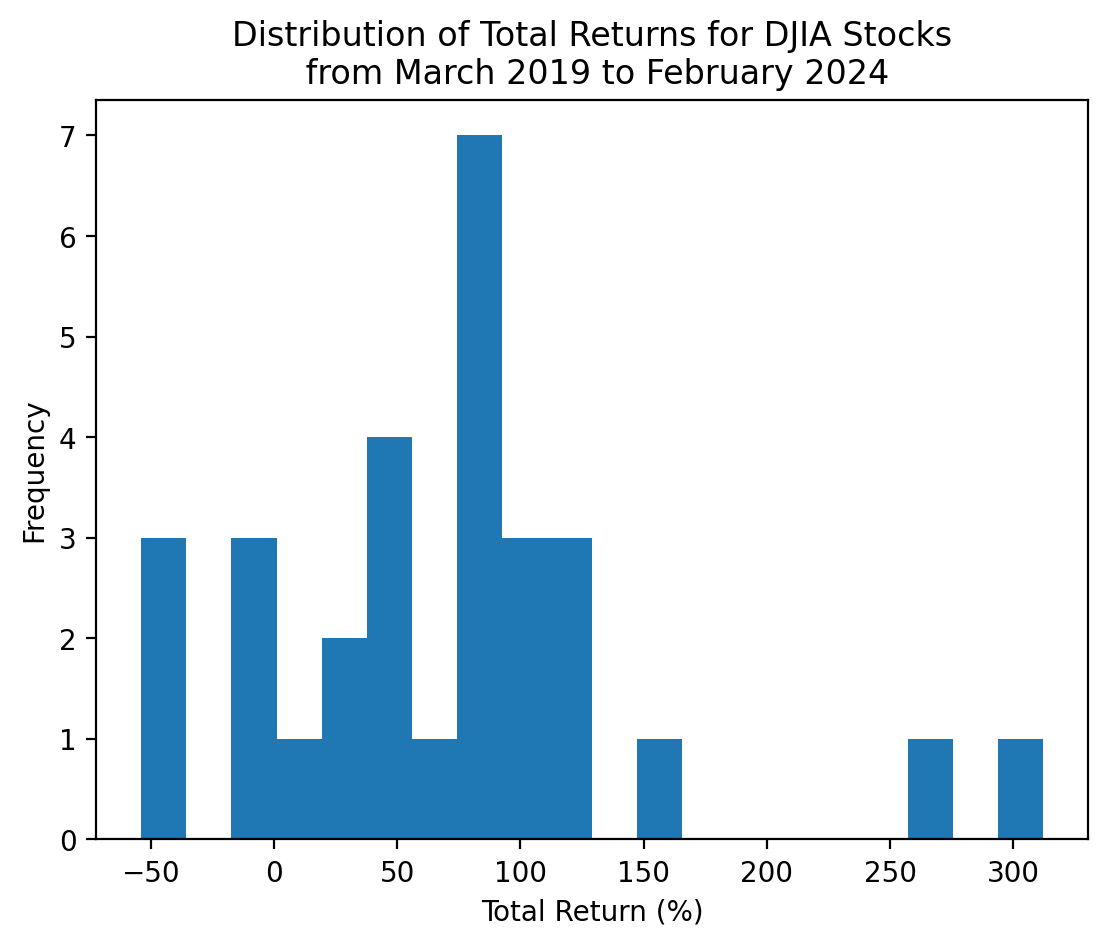
\includegraphics{mckinney_05_practice_03_files/figure-pdf/cell-25-output-1.png}

}

\end{figure}

With only 30 stocks, we can visualize and interpret each stock
separately!

\begin{Shaded}
\begin{Highlighting}[]
\NormalTok{start\_date }\OperatorTok{=}\NormalTok{ returns2.index.}\BuiltInTok{min}\NormalTok{()}
\NormalTok{stop\_date }\OperatorTok{=}\NormalTok{ returns2.index.}\BuiltInTok{max}\NormalTok{()}

\NormalTok{(}
\NormalTok{    returns2}
\NormalTok{    .add(}\DecValTok{1}\NormalTok{)}
\NormalTok{    .prod()}
\NormalTok{    .sub(}\DecValTok{1}\NormalTok{)}
\NormalTok{    .mul(}\DecValTok{100}\NormalTok{)}
\NormalTok{    .sort\_values()}
\NormalTok{    .plot(kind}\OperatorTok{=}\StringTok{\textquotesingle{}barh\textquotesingle{}}\NormalTok{, grid}\OperatorTok{=}\VariableTok{True}\NormalTok{)}
\NormalTok{)}
\NormalTok{plt.xlabel(}\StringTok{\textquotesingle{}Total Return (\%)\textquotesingle{}}\NormalTok{)}
\NormalTok{plt.title(}\SpecialStringTok{f\textquotesingle{}Total Returns for DJIA Stocks}\CharTok{\textbackslash{}n}\SpecialStringTok{ from }\SpecialCharTok{\{}\NormalTok{start\_date}\SpecialCharTok{:}\OperatorTok{\%}\NormalTok{B }\OperatorTok{\%}\NormalTok{Y}\SpecialCharTok{\}}\SpecialStringTok{ to }\SpecialCharTok{\{}\NormalTok{stop\_date}\SpecialCharTok{:}\OperatorTok{\%}\NormalTok{B }\OperatorTok{\%}\NormalTok{Y}\SpecialCharTok{\}}\SpecialStringTok{\textquotesingle{}}\NormalTok{)}
\NormalTok{plt.show()}
\end{Highlighting}
\end{Shaded}

\begin{figure}[H]

{\centering 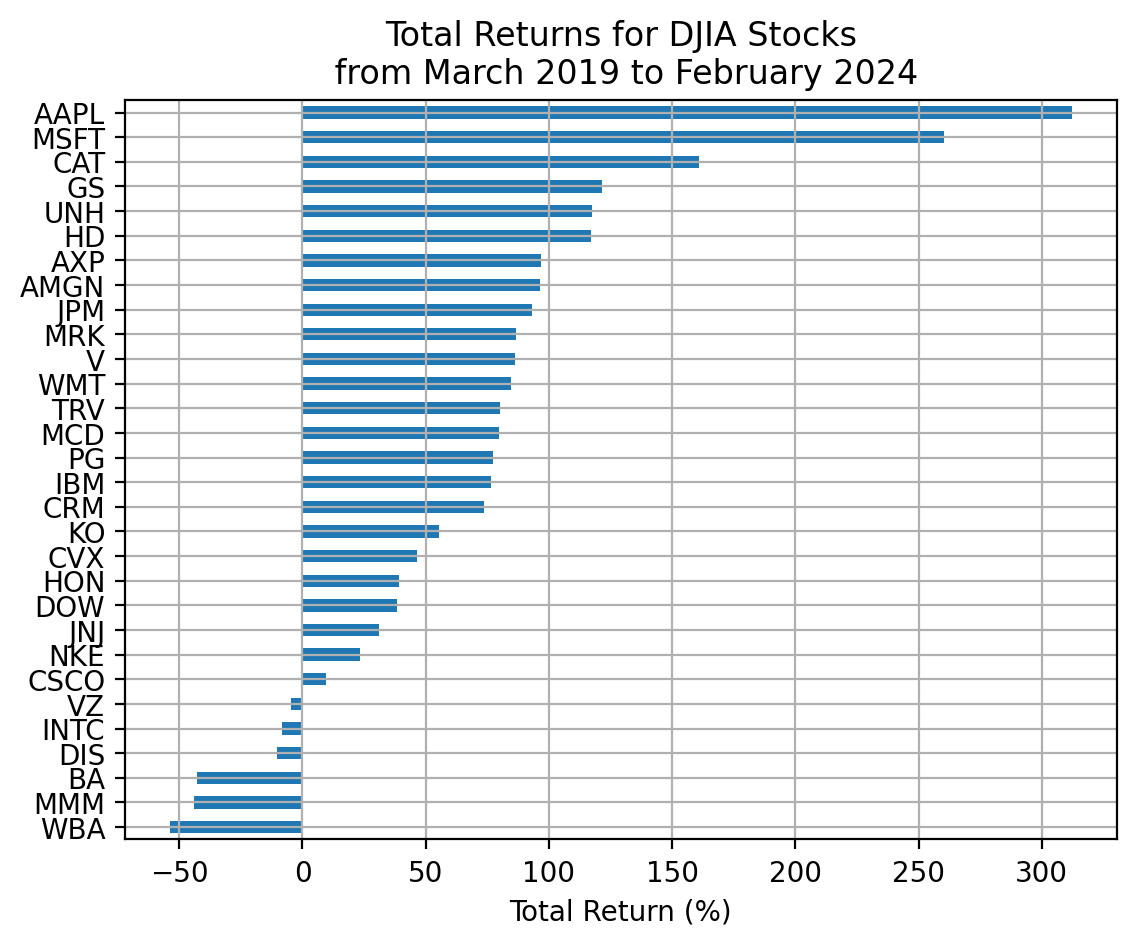
\includegraphics{mckinney_05_practice_03_files/figure-pdf/cell-26-output-1.png}

}

\end{figure}

\hypertarget{which-stocks-have-the-minimum-and-maximum-total-returns-1}{%
\subsection{Which stocks have the minimum and maximum total
returns?}\label{which-stocks-have-the-minimum-and-maximum-total-returns-1}}

If we want the \emph{values}, the \texttt{.min()} and \texttt{.max()}
methods are the way to go!

\begin{Shaded}
\begin{Highlighting}[]
\NormalTok{total\_returns2.}\BuiltInTok{min}\NormalTok{()}
\end{Highlighting}
\end{Shaded}

\begin{verbatim}
-0.5384
\end{verbatim}

\begin{Shaded}
\begin{Highlighting}[]
\NormalTok{total\_returns2.}\BuiltInTok{max}\NormalTok{()}
\end{Highlighting}
\end{Shaded}

\begin{verbatim}
3.1210
\end{verbatim}

The \texttt{.min()} and \texttt{.max()} methods give the values but not
the tickers (or index). We use the \texttt{.idxmin()} and
\texttt{.idxmax()} to get the tickers (or index).

\begin{Shaded}
\begin{Highlighting}[]
\NormalTok{total\_returns2.idxmin()}
\end{Highlighting}
\end{Shaded}

\begin{verbatim}
'WBA'
\end{verbatim}

\begin{Shaded}
\begin{Highlighting}[]
\NormalTok{total\_returns2.idxmax()}
\end{Highlighting}
\end{Shaded}

\begin{verbatim}
'AAPL'
\end{verbatim}

Here is what I would use!

\begin{Shaded}
\begin{Highlighting}[]
\NormalTok{total\_returns2.sort\_values().iloc[[}\DecValTok{0}\NormalTok{, }\OperatorTok{{-}}\DecValTok{1}\NormalTok{]]}
\end{Highlighting}
\end{Shaded}

\begin{verbatim}
WBA    -0.5384
AAPL    3.1210
dtype: float64
\end{verbatim}

Not the exactly right tool here, but the
\texttt{.nsmallest()\textquotesingle{}\ and}.nlargest()` methods are
really useful!

\begin{Shaded}
\begin{Highlighting}[]
\NormalTok{total\_returns2.nsmallest(}\DecValTok{3}\NormalTok{)}
\end{Highlighting}
\end{Shaded}

\begin{verbatim}
WBA   -0.5384
MMM   -0.4408
BA    -0.4289
dtype: float64
\end{verbatim}

\begin{Shaded}
\begin{Highlighting}[]
\NormalTok{total\_returns2.nlargest(}\DecValTok{3}\NormalTok{)}
\end{Highlighting}
\end{Shaded}

\begin{verbatim}
AAPL   3.1210
MSFT   2.6028
CAT    1.6083
dtype: float64
\end{verbatim}

\hypertarget{plot-the-cumulative-returns-for-the-stocks-in-the-djia-1}{%
\subsection{Plot the cumulative returns for the stocks in the
DJIA}\label{plot-the-cumulative-returns-for-the-stocks-in-the-djia-1}}

We can use the cumulative product method \texttt{.cumprod()} to
calculate the right hand side of the formula above.

\begin{Shaded}
\begin{Highlighting}[]
\NormalTok{start\_date }\OperatorTok{=}\NormalTok{ returns2.index.}\BuiltInTok{min}\NormalTok{()}
\NormalTok{stop\_date }\OperatorTok{=}\NormalTok{ returns2.index.}\BuiltInTok{max}\NormalTok{()}

\NormalTok{(}
\NormalTok{    returns2}
\NormalTok{    .add(}\DecValTok{1}\NormalTok{)}
\NormalTok{    .cumprod()}
\NormalTok{    .sub(}\DecValTok{1}\NormalTok{)}
\NormalTok{    .mul(}\DecValTok{100}\NormalTok{)}
\NormalTok{    .plot(legend}\OperatorTok{=}\VariableTok{False}\NormalTok{)}
\NormalTok{)}
\NormalTok{plt.xlabel(}\StringTok{\textquotesingle{}Cumulative Return (\%)\textquotesingle{}}\NormalTok{)}
\NormalTok{plt.title(}\SpecialStringTok{f\textquotesingle{}Cumulative Returns for DJIA Stocks}\CharTok{\textbackslash{}n}\SpecialStringTok{ from }\SpecialCharTok{\{}\NormalTok{start\_date}\SpecialCharTok{:}\OperatorTok{\%}\NormalTok{B }\OperatorTok{\%}\NormalTok{Y}\SpecialCharTok{\}}\SpecialStringTok{ to }\SpecialCharTok{\{}\NormalTok{stop\_date}\SpecialCharTok{:}\OperatorTok{\%}\NormalTok{B }\OperatorTok{\%}\NormalTok{Y}\SpecialCharTok{\}}\SpecialStringTok{\textquotesingle{}}\NormalTok{)}
\NormalTok{plt.show()}
\end{Highlighting}
\end{Shaded}

\begin{figure}[H]

{\centering 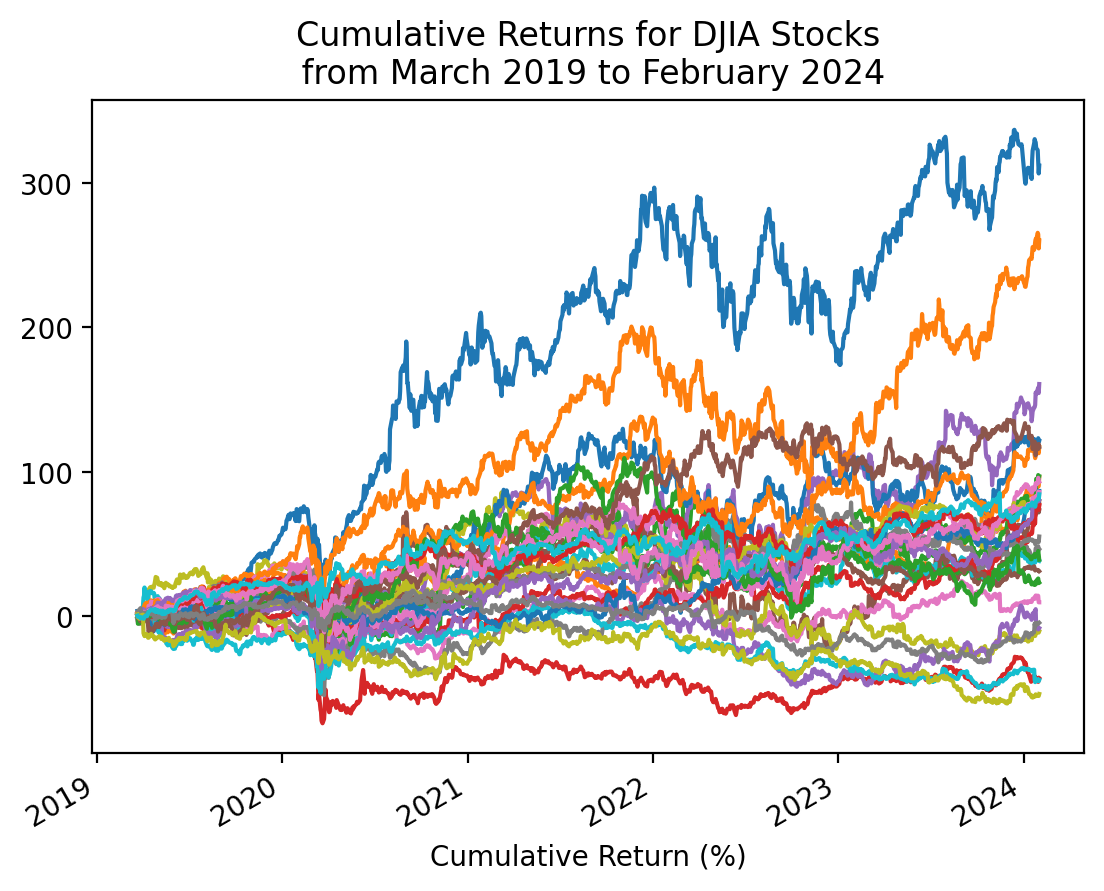
\includegraphics{mckinney_05_practice_03_files/figure-pdf/cell-34-output-1.png}

}

\end{figure}

\hypertarget{repeat-the-plot-above-with-only-the-minimum-and-maximum-total-returns-1}{%
\subsection{Repeat the plot above with only the minimum and maximum
total
returns}\label{repeat-the-plot-above-with-only-the-minimum-and-maximum-total-returns-1}}

\begin{Shaded}
\begin{Highlighting}[]
\NormalTok{total\_returns2.sort\_values().iloc[[}\DecValTok{0}\NormalTok{, }\OperatorTok{{-}}\DecValTok{1}\NormalTok{]].index}
\end{Highlighting}
\end{Shaded}

\begin{verbatim}
Index(['WBA', 'AAPL'], dtype='object')
\end{verbatim}

\begin{Shaded}
\begin{Highlighting}[]
\NormalTok{start\_date }\OperatorTok{=}\NormalTok{ returns2.index.}\BuiltInTok{min}\NormalTok{()}
\NormalTok{stop\_date }\OperatorTok{=}\NormalTok{ returns2.index.}\BuiltInTok{max}\NormalTok{()}

\NormalTok{(}
\NormalTok{    returns2[total\_returns2.sort\_values().iloc[[}\DecValTok{0}\NormalTok{, }\OperatorTok{{-}}\DecValTok{1}\NormalTok{]].index]}
\NormalTok{    .add(}\DecValTok{1}\NormalTok{)}
\NormalTok{    .cumprod()}
\NormalTok{    .sub(}\DecValTok{1}\NormalTok{)}
\NormalTok{    .mul(}\DecValTok{100}\NormalTok{)}
\NormalTok{    .plot()}
\NormalTok{)}
\NormalTok{plt.xlabel(}\StringTok{\textquotesingle{}Cumulative Return (\%)\textquotesingle{}}\NormalTok{)}
\NormalTok{plt.title(}\SpecialStringTok{f\textquotesingle{}Cumulative Returns for DJIA Stocks}\CharTok{\textbackslash{}n}\SpecialStringTok{ from }\SpecialCharTok{\{}\NormalTok{start\_date}\SpecialCharTok{:}\OperatorTok{\%}\NormalTok{B }\OperatorTok{\%}\NormalTok{Y}\SpecialCharTok{\}}\SpecialStringTok{ to }\SpecialCharTok{\{}\NormalTok{stop\_date}\SpecialCharTok{:}\OperatorTok{\%}\NormalTok{B }\OperatorTok{\%}\NormalTok{Y}\SpecialCharTok{\}}\SpecialStringTok{\textquotesingle{}}\NormalTok{)}
\NormalTok{plt.show()}
\end{Highlighting}
\end{Shaded}

\begin{figure}[H]

{\centering 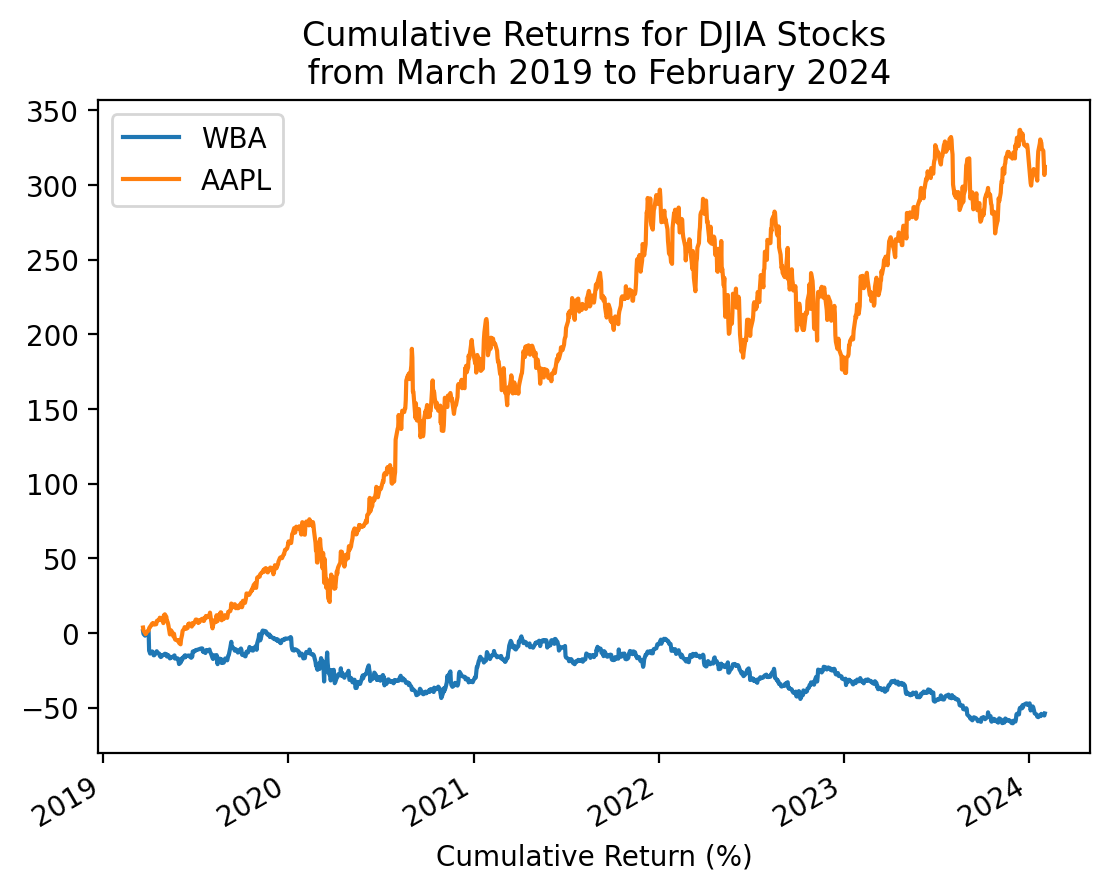
\includegraphics{mckinney_05_practice_03_files/figure-pdf/cell-36-output-1.png}

}

\end{figure}

\hypertarget{mckinney-chapter-5---practice-for-section-04}{%
\chapter{McKinney Chapter 5 - Practice for Section
04}\label{mckinney-chapter-5---practice-for-section-04}}

\hypertarget{announcements-14}{%
\section{Announcements}\label{announcements-14}}

\begin{enumerate}
\def\labelenumi{\arabic{enumi}.}
\tightlist
\item
  No DataCamp this week, but I suggest you keep working on it
\item
  Keep forming groups, and I will post our first project early next week
\end{enumerate}

\hypertarget{minute-recap-13}\NormalTok{precision }\DecValTok{4}
\NormalTok{pd.options.display.float\_format }\OperatorTok{=} \StringTok{\textquotesingle{}}\SpecialCharTok{\{:.4f\}}\StringTok{\textquotesingle{}}\NormalTok{.}\BuiltInTok{format}
\OperatorTok{\%}\NormalTok{config InlineBackend.figure\_format }\OperatorTok{=} \StringTok{\textquotesingle{}retina\textquotesingle{}}
\end{Highlighting}
\end{Shaded}

pandas provides two data structures:

\begin{enumerate}
\def\labelenumi{\arabic{enumi}.}
\tightlist
\item
  Data frame is a 2-D, mixed data type structure, like a worksheet in an
  Excel workbook
\item
  Series is a 1-D, one data type structure, like a column in a worksheet
  (or data frame)
\end{enumerate}

\begin{Shaded}
\begin{Highlighting}[]
\NormalTok{np.random.seed(}\DecValTok{42}\NormalTok{)}
\NormalTok{df }\OperatorTok{=}\NormalTok{ pd.DataFrame(}
\NormalTok{    data}\OperatorTok{=}\NormalTok{np.random.randn(}\DecValTok{3}\NormalTok{, }\DecValTok{4}\NormalTok{), }\CommentTok{\# 12 random numbers}
\NormalTok{    index}\OperatorTok{=}\BuiltInTok{list}\NormalTok{(}\StringTok{\textquotesingle{}ABC\textquotesingle{}}\NormalTok{), }\CommentTok{\# labels the rows for easy indexing and slicing}
\NormalTok{    columns}\OperatorTok{=}\BuiltInTok{list}\NormalTok{(}\StringTok{\textquotesingle{}abcd\textquotesingle{}}\NormalTok{) }\CommentTok{\# labels the columns for easy indexing and slicing}
\NormalTok{)}

\NormalTok{df}
\end{Highlighting}
\end{Shaded}

\begin{longtable}[]{@{}lllll@{}}
\toprule\noalign{}
& a & b & c & d \\
\midrule\noalign{}
\endhead
\bottomrule\noalign{}
\endlastfoot
A & 0.4967 & -0.1383 & 0.6477 & 1.5230 \\
B & -0.2342 & -0.2341 & 1.5792 & 0.7674 \\
C & -0.4695 & 0.5426 & -0.4634 & -0.4657 \\
\end{longtable}

How do we index or slice data frames?

\begin{enumerate}
\def\labelenumi{\arabic{enumi}.}
\tightlist
\item
  With integer locations and the \texttt{.iloc{[}{]}} method
\item
  With row and column names and the \texttt{.loc{[}{]}} method
\end{enumerate}

Say we want the first two rows and first three columns.

\begin{Shaded}
\begin{Highlighting}[]
\NormalTok{df.iloc[:}\DecValTok{2}\NormalTok{, :}\DecValTok{3}\NormalTok{] }\CommentTok{\# j,k slicing, as in NumPy}
\end{Highlighting}
\end{Shaded}

\begin{longtable}[]{@{}llll@{}}
\toprule\noalign{}
& a & b & c \\
\midrule\noalign{}
\endhead
\bottomrule\noalign{}
\endlastfoot
A & 0.4967 & -0.1383 & 0.6477 \\
B & -0.2342 & -0.2341 & 1.5792 \\
\end{longtable}

\begin{Shaded}
\begin{Highlighting}[]
\NormalTok{df.loc[[}\StringTok{\textquotesingle{}A\textquotesingle{}}\NormalTok{, }\StringTok{\textquotesingle{}B\textquotesingle{}}\NormalTok{], [}\StringTok{\textquotesingle{}a\textquotesingle{}}\NormalTok{, }\StringTok{\textquotesingle{}b\textquotesingle{}}\NormalTok{, }\StringTok{\textquotesingle{}c\textquotesingle{}}\NormalTok{]]}
\end{Highlighting}
\end{Shaded}

\begin{longtable}[]{@{}llll@{}}
\toprule\noalign{}
& a & b & c \\
\midrule\noalign{}
\endhead
\bottomrule\noalign{}
\endlastfoot
A & 0.4967 & -0.1383 & 0.6477 \\
B & -0.2342 & -0.2341 & 1.5792 \\
\end{longtable}

\textbf{\emph{Both left and right edges of named slices are included in
pandas!}}

\begin{Shaded}
\begin{Highlighting}[]
\NormalTok{df.loc[}\StringTok{\textquotesingle{}A\textquotesingle{}}\NormalTok{:}\StringTok{\textquotesingle{}B\textquotesingle{}}\NormalTok{, }\StringTok{\textquotesingle{}a\textquotesingle{}}\NormalTok{:}\StringTok{\textquotesingle{}c\textquotesingle{}}\NormalTok{]}
\end{Highlighting}
\end{Shaded}

\begin{longtable}[]{@{}llll@{}}
\toprule\noalign{}
& a & b & c \\
\midrule\noalign{}
\endhead
\bottomrule\noalign{}
\endlastfoot
A & 0.4967 & -0.1383 & 0.6477 \\
B & -0.2342 & -0.2341 & 1.5792 \\
\end{longtable}

How do I add a column?

\begin{Shaded}
\begin{Highlighting}[]
\NormalTok{df[}\StringTok{\textquotesingle{}e\textquotesingle{}}\NormalTok{] }\OperatorTok{=} \DecValTok{5} \CommentTok{\# pandas broadcasts this 5 to all rows}

\NormalTok{df}
\end{Highlighting}
\end{Shaded}

\begin{longtable}[]{@{}llllll@{}}
\toprule\noalign{}
& a & b & c & d & e \\
\midrule\noalign{}
\endhead
\bottomrule\noalign{}
\endlastfoot
A & 0.4967 & -0.1383 & 0.6477 & 1.5230 & 5 \\
B & -0.2342 & -0.2341 & 1.5792 & 0.7674 & 5 \\
C & -0.4695 & 0.5426 & -0.4634 & -0.4657 & 5 \\
\end{longtable}

A series is the other data structure.

\begin{Shaded}
\begin{Highlighting}[]
\NormalTok{ser }\OperatorTok{=}\NormalTok{ pd.Series(data}\OperatorTok{=}\NormalTok{np.arange(}\FloatTok{2.}\NormalTok{), index}\OperatorTok{=}\BuiltInTok{list}\NormalTok{(}\StringTok{\textquotesingle{}BC\textquotesingle{}}\NormalTok{))}

\NormalTok{ser}
\end{Highlighting}
\end{Shaded}

\begin{verbatim}
B   0.0000
C   1.0000
dtype: float64
\end{verbatim}

\begin{Shaded}
\begin{Highlighting}[]
\NormalTok{df[}\StringTok{\textquotesingle{}f\textquotesingle{}}\NormalTok{] }\OperatorTok{=}\NormalTok{ ser}

\NormalTok{df}
\end{Highlighting}
\end{Shaded}

\begin{longtable}[]{@{}lllllll@{}}
\toprule\noalign{}
& a & b & c & d & e & f \\
\midrule\noalign{}
\endhead
\bottomrule\noalign{}
\endlastfoot
A & 0.4967 & -0.1383 & 0.6477 & 1.5230 & 5 & NaN \\
B & -0.2342 & -0.2341 & 1.5792 & 0.7674 & 5 & 0.0000 \\
C & -0.4695 & 0.5426 & -0.4634 & -0.4657 & 5 & 1.0000 \\
\end{longtable}

\hypertarget{practice-14}{%
\section{Practice}\label{practice-14}}

\begin{Shaded}
\begin{Highlighting}[]
\NormalTok{tickers }\OperatorTok{=} \StringTok{\textquotesingle{}AAPL IBM MSFT GOOG\textquotesingle{}}
\NormalTok{prices }\OperatorTok{=}\NormalTok{ yf.download(tickers}\OperatorTok{=}\NormalTok{tickers)}
\end{Highlighting}
\end{Shaded}

\begin{verbatim}
[*********************100%%**********************]  4 of 4 completed
\end{verbatim}

\begin{Shaded}
\begin{Highlighting}[]
\NormalTok{returns }\OperatorTok{=}\NormalTok{ (}
\NormalTok{    prices[}\StringTok{\textquotesingle{}Adj Close\textquotesingle{}}\NormalTok{] }\CommentTok{\# slices the adj close columns}
\NormalTok{    .iloc[:}\OperatorTok{{-}}\DecValTok{1}\NormalTok{] }\CommentTok{\# drop last date with intraday price}
\NormalTok{    .pct\_change() }\CommentTok{\# calculate returns}
\NormalTok{    .dropna() }\CommentTok{\# drop dates with incomplete returns data}
\NormalTok{)}

\NormalTok{returns}
\end{Highlighting}
\end{Shaded}

\begin{longtable}[]{@{}lllll@{}}
\toprule\noalign{}
& AAPL & GOOG & IBM & MSFT \\
Date & & & & \\
\midrule\noalign{}
\endhead
\bottomrule\noalign{}
\endlastfoot
2004-08-20 & 0.0029 & 0.0794 & 0.0042 & 0.0030 \\
2004-08-23 & 0.0091 & 0.0101 & -0.0070 & 0.0044 \\
2004-08-24 & 0.0280 & -0.0414 & 0.0007 & 0.0000 \\
2004-08-25 & 0.0344 & 0.0108 & 0.0042 & 0.0114 \\
2004-08-26 & 0.0487 & 0.0180 & -0.0045 & -0.0040 \\
... & ... & ... & ... & ... \\
2024-01-26 & -0.0090 & 0.0010 & -0.0158 & -0.0023 \\
2024-01-29 & -0.0036 & 0.0068 & -0.0015 & 0.0143 \\
2024-01-30 & -0.0192 & -0.0116 & 0.0039 & -0.0028 \\
2024-01-31 & -0.0194 & -0.0735 & -0.0224 & -0.0269 \\
2024-02-01 & 0.0133 & 0.0064 & 0.0176 & 0.0156 \\
\end{longtable}

\hypertarget{what-are-the-mean-daily-returns-for-these-four-stocks-2}{%
\subsection{What are the mean daily returns for these four
stocks?}\label{what-are-the-mean-daily-returns-for-these-four-stocks-2}}

\begin{Shaded}
\begin{Highlighting}[]
\NormalTok{returns.mean() }\CommentTok{\# default is axis=0}
\end{Highlighting}
\end{Shaded}

\begin{verbatim}
AAPL   0.0014
GOOG   0.0010
IBM    0.0004
MSFT   0.0008
dtype: float64
\end{verbatim}

If we use \texttt{.mean(axis=1)} on stock returns, we get the
equallu-weighted portfolio returns on each day.

\begin{Shaded}
\begin{Highlighting}[]
\NormalTok{returns.mean(axis}\OperatorTok{=}\DecValTok{1}\NormalTok{)}
\end{Highlighting}
\end{Shaded}

\begin{verbatim}
Date
2004-08-20    0.0224
2004-08-23    0.0041
2004-08-24   -0.0032
2004-08-25    0.0152
2004-08-26    0.0146
               ...  
2024-01-26   -0.0065
2024-01-29    0.0040
2024-01-30   -0.0074
2024-01-31   -0.0356
2024-02-01    0.0132
Length: 4896, dtype: float64
\end{verbatim}

\hypertarget{what-are-the-standard-deviations-of-daily-returns-for-these-four-stocks-2}{%
\subsection{What are the standard deviations of daily returns for these
four
stocks?}\label{what-are-the-standard-deviations-of-daily-returns-for-these-four-stocks-2}}

pandas methods give us \emph{sample} statistics, instead of population
statistics in NumPy.

\begin{Shaded}
\begin{Highlighting}[]
\NormalTok{returns.std()}
\end{Highlighting}
\end{Shaded}

\begin{verbatim}
AAPL   0.0206
GOOG   0.0194
IBM    0.0143
MSFT   0.0171
dtype: float64
\end{verbatim}

\hypertarget{what-are-the-annualized-means-and-standard-deviations-of-daily-returns-for-these-four-stocks-2}{%
\subsection{\texorpdfstring{What are the \emph{annualized} means and
standard deviations of daily returns for these four
stocks?}{What are the annualized means and standard deviations of daily returns for these four stocks?}}\label{what-are-the-annualized-means-and-standard-deviations-of-daily-returns-for-these-four-stocks-2}}

We annualize mean returns by multiplying by \(T\) (\(T=252\) for daily
returns, \(T=12\) for month returns, and so on). We annualize standard
deviations by multiplying by \(\sqrt(T)\).

\begin{Shaded}
\begin{Highlighting}[]
\NormalTok{returns.mean().mul(}\DecValTok{252}\NormalTok{)}
\end{Highlighting}
\end{Shaded}

\begin{verbatim}
AAPL   0.3625
GOOG   0.2552
IBM    0.0980
MSFT   0.2002
dtype: float64
\end{verbatim}

\begin{Shaded}
\begin{Highlighting}[]
\NormalTok{returns.std().mul(np.sqrt(}\DecValTok{252}\NormalTok{))}
\end{Highlighting}
\end{Shaded}

\begin{verbatim}
AAPL   0.3276
GOOG   0.3074
IBM    0.2272
MSFT   0.2722
dtype: float64
\end{verbatim}

\hypertarget{plot-annualized-means-versus-standard-deviations-of-daily-returns-for-these-four-stocks-2}{%
\subsection{\texorpdfstring{Plot \emph{annualized} means versus standard
deviations of daily returns for these four
stocks}{Plot annualized means versus standard deviations of daily returns for these four stocks}}\label{plot-annualized-means-versus-standard-deviations-of-daily-returns-for-these-four-stocks-2}}

\begin{Shaded}
\begin{Highlighting}[]
\NormalTok{means }\OperatorTok{=}\NormalTok{ returns.mean().mul(}\DecValTok{252} \OperatorTok{*} \DecValTok{100}\NormalTok{)}
\NormalTok{vols }\OperatorTok{=}\NormalTok{ returns.std().mul(np.sqrt(}\DecValTok{252}\NormalTok{) }\OperatorTok{*} \DecValTok{100}\NormalTok{)}

\NormalTok{plt.scatter(}
\NormalTok{    x}\OperatorTok{=}\NormalTok{vols,}
\NormalTok{    y}\OperatorTok{=}\NormalTok{means}
\NormalTok{)}

\CommentTok{\# add tickers to each point}
\ControlFlowTok{for}\NormalTok{ i }\KeywordTok{in}\NormalTok{ means.index: }\CommentTok{\# loop over ticker index}
\NormalTok{    plt.text( }\CommentTok{\# plots string s at coordinates x and y}
\NormalTok{        x}\OperatorTok{=}\NormalTok{vols[i], }\CommentTok{\# indexes volatility}
\NormalTok{        y}\OperatorTok{=}\NormalTok{means[i], }\CommentTok{\# indexes mean return}
\NormalTok{        s}\OperatorTok{=}\NormalTok{i }\CommentTok{\# ticker index}
\NormalTok{    )}

\NormalTok{plt.xlabel(}\StringTok{\textquotesingle{}Annualized Volatility of Daily Returns (\%)\textquotesingle{}}\NormalTok{)}
\NormalTok{plt.ylabel(}\StringTok{\textquotesingle{}Annualized Means of Daily Returns (\%)\textquotesingle{}}\NormalTok{)}
\NormalTok{plt.title(}\StringTok{\textquotesingle{}Returns versus Risk\textquotesingle{}}\NormalTok{)}
\NormalTok{plt.show()}
\end{Highlighting}
\end{Shaded}

\begin{figure}[H]

{\centering 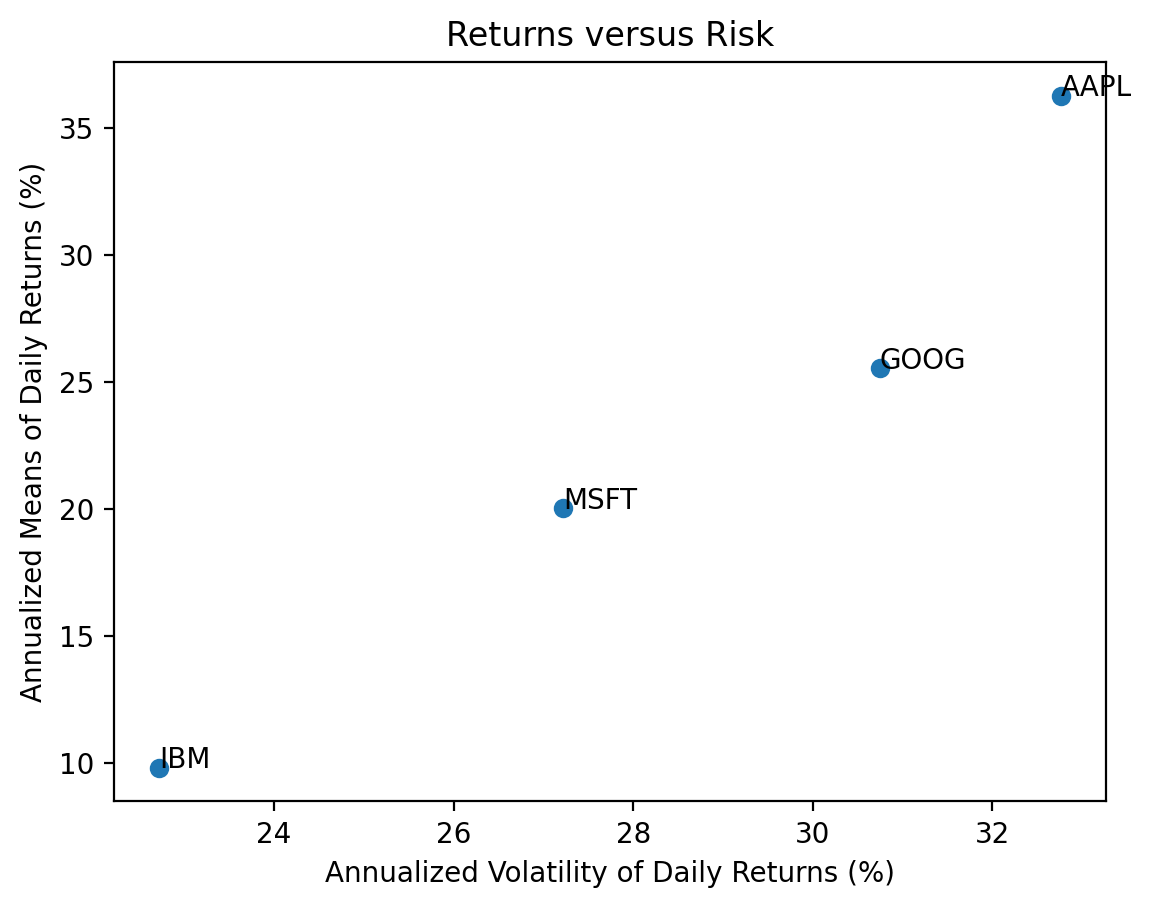
\includegraphics{mckinney_05_practice_04_files/figure-pdf/cell-18-output-1.png}

}

\end{figure}

Use \texttt{plt.scatter()}, which expects arguments as \texttt{x}
(standard deviations) then \texttt{y} (means).

\hypertarget{repeat-the-previous-calculations-and-plot-for-the-stocks-in-the-dow-jones-industrial-index-djia-2}{%
\subsection{Repeat the previous calculations and plot for the stocks in
the Dow-Jones Industrial Index
(DJIA)}\label{repeat-the-previous-calculations-and-plot-for-the-stocks-in-the-dow-jones-industrial-index-djia-2}}

We can find the current DJIA stocks on
\href{https://en.wikipedia.org/wiki/Dow_Jones_Industrial_Average}{Wikipedia}.
We will need to download new data, into \texttt{tickers2},
\texttt{prices2}, and \texttt{returns2}.

\begin{Shaded}
\begin{Highlighting}[]
\NormalTok{url2 }\OperatorTok{=} \StringTok{\textquotesingle{}https://en.wikipedia.org/wiki/Dow\_Jones\_Industrial\_Average\textquotesingle{}}
\NormalTok{wiki2 }\OperatorTok{=}\NormalTok{ pd.read\_html(url2)}
\NormalTok{tickers2 }\OperatorTok{=}\NormalTok{ wiki2[}\DecValTok{1}\NormalTok{][}\StringTok{\textquotesingle{}Symbol\textquotesingle{}}\NormalTok{].to\_list()}
\NormalTok{tickers2[:}\DecValTok{5}\NormalTok{]}
\end{Highlighting}
\end{Shaded}

\begin{verbatim}
['MMM', 'AXP', 'AMGN', 'AAPL', 'BA']
\end{verbatim}

\begin{Shaded}
\begin{Highlighting}[]
\NormalTok{prices2 }\OperatorTok{=}\NormalTok{ yf.download(tickers}\OperatorTok{=}\NormalTok{tickers2)}
\end{Highlighting}
\end{Shaded}

\begin{verbatim}
[*********************100%%**********************]  30 of 30 completed
\end{verbatim}

\begin{Shaded}
\begin{Highlighting}[]
\NormalTok{returns2 }\OperatorTok{=}\NormalTok{ (}
\NormalTok{    prices2[}\StringTok{\textquotesingle{}Adj Close\textquotesingle{}}\NormalTok{]}
\NormalTok{    .iloc[:}\OperatorTok{{-}}\DecValTok{1}\NormalTok{]}
\NormalTok{    .pct\_change()}
\NormalTok{    .dropna()}
\NormalTok{)}

\NormalTok{returns2}
\end{Highlighting}
\end{Shaded}

\begin{longtable}[]{@{}llllllllllllllllllllll@{}}
\toprule\noalign{}
& AAPL & AMGN & AXP & BA & CAT & CRM & CSCO & CVX & DIS & DOW & ... &
MRK & MSFT & NKE & PG & TRV & UNH & V & VZ & WBA & WMT \\
Date & & & & & & & & & & & & & & & & & & & & & \\
\midrule\noalign{}
\endhead
\bottomrule\noalign{}
\endlastfoot
2019-03-21 & 0.0368 & 0.0040 & 0.0095 & -0.0092 & 0.0079 & 0.0210 &
0.0128 & 0.0094 & -0.0121 & -0.0165 & ... & 0.0106 & 0.0230 & 0.0152 &
0.0076 & 0.0231 & 0.0061 & 0.0133 & 0.0108 & 0.0129 & 0.0043 \\
2019-03-22 & -0.0207 & -0.0270 & -0.0211 & -0.0283 & -0.0320 & -0.0326 &
-0.0222 & -0.0220 & -0.0040 & -0.0078 & ... & -0.0080 & -0.0264 &
-0.0661 & -0.0081 & 0.0039 & -0.0196 & -0.0175 & 0.0252 & -0.0187 &
-0.0079 \\
2019-03-25 & -0.0121 & -0.0006 & -0.0038 & 0.0229 & 0.0124 & -0.0038 &
-0.0002 & -0.0016 & -0.0041 & 0.0113 & ... & 0.0007 & 0.0052 & 0.0017 &
0.0030 & 0.0004 & -0.0009 & -0.0003 & 0.0054 & -0.0115 & -0.0011 \\
2019-03-26 & -0.0103 & 0.0090 & 0.0042 & -0.0002 & 0.0035 & -0.0092 &
0.0095 & 0.0101 & 0.0218 & -0.0061 & ... & 0.0069 & 0.0021 & 0.0128 &
0.0104 & 0.0002 & -0.0141 & 0.0148 & 0.0092 & 0.0037 & 0.0015 \\
2019-03-27 & 0.0090 & -0.0104 & -0.0047 & 0.0103 & -0.0049 & -0.0269 &
-0.0017 & -0.0108 & 0.0013 & 0.0256 & ... & -0.0076 & -0.0097 & -0.0035
& -0.0012 & 0.0101 & -0.0069 & -0.0070 & 0.0041 & 0.0050 & -0.0113 \\
... & ... & ... & ... & ... & ... & ... & ... & ... & ... & ... & ... &
... & ... & ... & ... & ... & ... & ... & ... & ... & ... \\
2024-01-26 & -0.0090 & 0.0049 & 0.0710 & 0.0178 & -0.0045 & 0.0033 &
-0.0036 & 0.0038 & 0.0053 & -0.0160 & ... & 0.0057 & -0.0023 & 0.0196 &
0.0033 & -0.0004 & 0.0199 & -0.0171 & 0.0026 & -0.0113 & 0.0088 \\
2024-01-29 & -0.0036 & 0.0054 & -0.0028 & -0.0014 & 0.0128 & 0.0283 &
0.0029 & -0.0004 & 0.0223 & 0.0002 & ... & 0.0038 & 0.0143 & 0.0110 &
0.0001 & -0.0015 & 0.0027 & 0.0213 & -0.0083 & -0.0057 & 0.0047 \\
2024-01-30 & -0.0192 & 0.0037 & 0.0164 & -0.0231 & 0.0050 & -0.0005 &
-0.0010 & 0.0070 & -0.0056 & 0.0074 & ... & 0.0031 & -0.0028 & 0.0029 &
0.0085 & 0.0115 & -0.0018 & 0.0128 & 0.0100 & 0.0018 & 0.0033 \\
2024-01-31 & -0.0194 & -0.0011 & -0.0167 & 0.0529 & -0.0146 & -0.0231 &
-0.0394 & -0.0179 & -0.0092 & -0.0160 & ... & -0.0072 & -0.0269 &
-0.0254 & -0.0022 & -0.0102 & 0.0161 & -0.0140 & -0.0028 & -0.0083 &
-0.0021 \\
2024-02-01 & 0.0133 & 0.0328 & 0.0124 & -0.0058 & 0.0246 & 0.0096 &
0.0000 & 0.0031 & 0.0105 & -0.0011 & ... & 0.0464 & 0.0156 & 0.0023 &
0.0130 & 0.0031 & -0.0090 & 0.0139 & 0.0033 & 0.0301 & 0.0185 \\
\end{longtable}

\begin{Shaded}
\begin{Highlighting}[]
\NormalTok{means }\OperatorTok{=}\NormalTok{ returns2.mean().mul(}\DecValTok{252} \OperatorTok{*} \DecValTok{100}\NormalTok{)}
\NormalTok{vols }\OperatorTok{=}\NormalTok{ returns2.std().mul(np.sqrt(}\DecValTok{252}\NormalTok{) }\OperatorTok{*} \DecValTok{100}\NormalTok{)}

\NormalTok{plt.scatter(}
\NormalTok{    x}\OperatorTok{=}\NormalTok{vols,}
\NormalTok{    y}\OperatorTok{=}\NormalTok{means}
\NormalTok{)}

\CommentTok{\# add tickers to each point}
\ControlFlowTok{for}\NormalTok{ i }\KeywordTok{in}\NormalTok{ means.index: }\CommentTok{\# loop over ticker index}
\NormalTok{    plt.text( }\CommentTok{\# plots string s at coordinates x and y}
\NormalTok{        x}\OperatorTok{=}\NormalTok{vols[i], }\CommentTok{\# indexes volatility}
\NormalTok{        y}\OperatorTok{=}\NormalTok{means[i], }\CommentTok{\# indexes mean return}
\NormalTok{        s}\OperatorTok{=}\NormalTok{i }\CommentTok{\# ticker index}
\NormalTok{    )}

\NormalTok{plt.xlabel(}\StringTok{\textquotesingle{}Annualized Volatility of Daily Returns (\%)\textquotesingle{}}\NormalTok{)}
\NormalTok{plt.ylabel(}\StringTok{\textquotesingle{}Annualized Means of Daily Returns (\%)\textquotesingle{}}\NormalTok{)}
\NormalTok{plt.title(}\StringTok{\textquotesingle{}Returns versus Risk\textquotesingle{}}\NormalTok{)}
\NormalTok{plt.show()}
\end{Highlighting}
\end{Shaded}

\begin{figure}[H]

{\centering 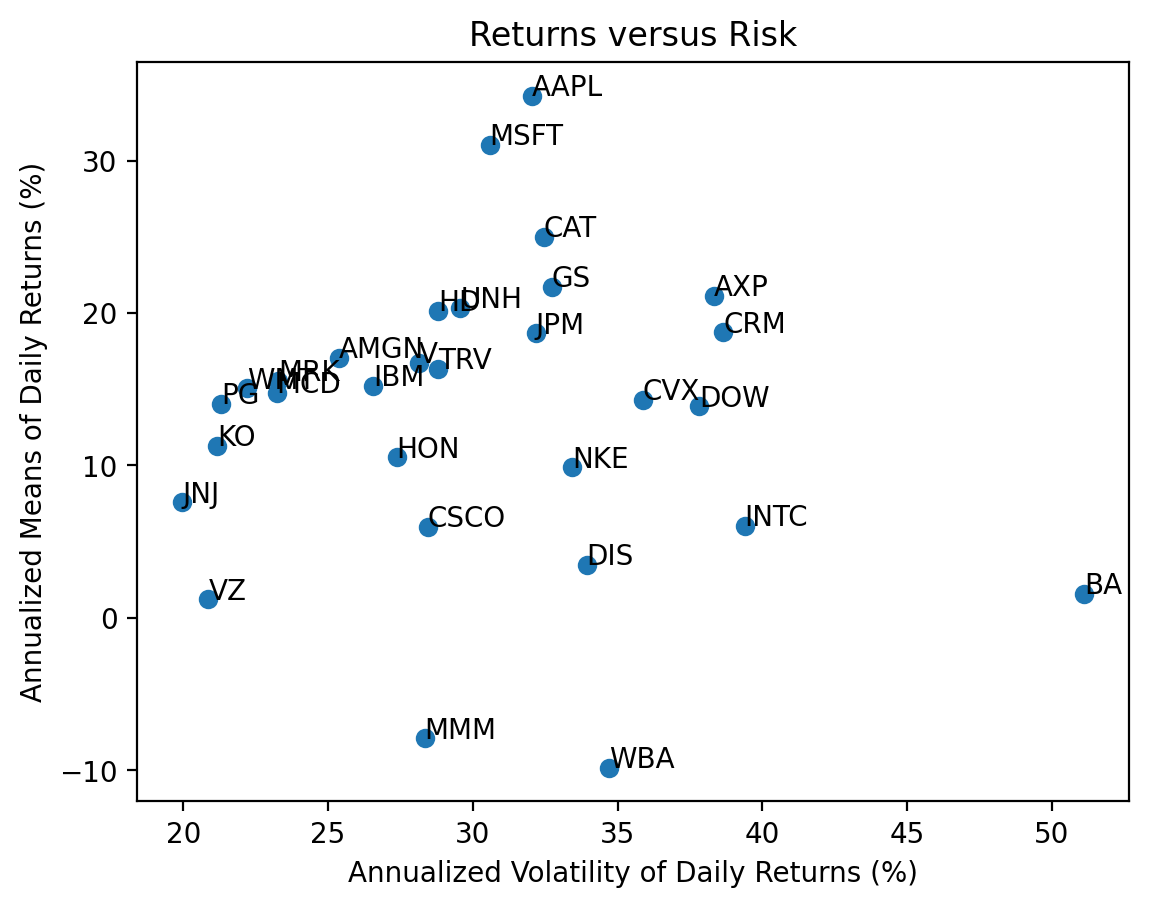
\includegraphics{mckinney_05_practice_04_files/figure-pdf/cell-22-output-1.png}

}

\end{figure}

\hypertarget{calculate-total-returns-for-the-stocks-in-the-djia-2}{%
\subsection{Calculate total returns for the stocks in the
DJIA}\label{calculate-total-returns-for-the-stocks-in-the-djia-2}}

We can use the \texttt{.prod()} method to compound returns as
\(1 + R_T = \prod_{t=1}^T (1 + R_t)\). Technically, we should write
\(R_T\) as \(R_{0,T}\), but we typically omit the subscript \(0\).

\begin{Shaded}
\begin{Highlighting}[]
\NormalTok{total\_returns2 }\OperatorTok{=}\NormalTok{ returns2.add(}\DecValTok{1}\NormalTok{).prod().sub(}\DecValTok{1}\NormalTok{)}
\NormalTok{total\_returns2.iloc[:}\DecValTok{5}\NormalTok{]}
\end{Highlighting}
\end{Shaded}

\begin{verbatim}
AAPL    3.1210
AMGN    0.9635
AXP     0.9687
BA     -0.4289
CAT     1.6083
dtype: float64
\end{verbatim}

\hypertarget{plot-the-distribution-of-total-returns-for-the-stocks-in-the-djia-2}{%
\subsection{Plot the distribution of total returns for the stocks in the
DJIA}\label{plot-the-distribution-of-total-returns-for-the-stocks-in-the-djia-2}}

We can plot a histogram, using either the \texttt{plt.hist()} function
or the \texttt{.plot(kind=\textquotesingle{}hist\textquotesingle{})}
method.

\begin{Shaded}
\begin{Highlighting}[]
\NormalTok{start\_date }\OperatorTok{=}\NormalTok{ returns2.index.}\BuiltInTok{min}\NormalTok{()}
\NormalTok{stop\_date }\OperatorTok{=}\NormalTok{ returns2.index.}\BuiltInTok{max}\NormalTok{()}

\NormalTok{(}
\NormalTok{    returns2}
\NormalTok{    .add(}\DecValTok{1}\NormalTok{)}
\NormalTok{    .prod()}
\NormalTok{    .sub(}\DecValTok{1}\NormalTok{)}
\NormalTok{    .mul(}\DecValTok{100}\NormalTok{)}
\NormalTok{    .plot(kind}\OperatorTok{=}\StringTok{\textquotesingle{}hist\textquotesingle{}}\NormalTok{, bins}\OperatorTok{=}\DecValTok{20}\NormalTok{)}
\NormalTok{)}
\NormalTok{plt.xlabel(}\StringTok{\textquotesingle{}Total Return (\%)\textquotesingle{}}\NormalTok{)}
\NormalTok{plt.title(}\SpecialStringTok{f\textquotesingle{}Distribution of Total Returns for DJIA Stocks}\CharTok{\textbackslash{}n}\SpecialStringTok{ from }\SpecialCharTok{\{}\NormalTok{start\_date}\SpecialCharTok{:}\OperatorTok{\%}\NormalTok{B }\OperatorTok{\%}\NormalTok{Y}\SpecialCharTok{\}}\SpecialStringTok{ to }\SpecialCharTok{\{}\NormalTok{stop\_date}\SpecialCharTok{:}\OperatorTok{\%}\NormalTok{B }\OperatorTok{\%}\NormalTok{Y}\SpecialCharTok{\}}\SpecialStringTok{\textquotesingle{}}\NormalTok{)}
\NormalTok{plt.show()}
\end{Highlighting}
\end{Shaded}

\begin{figure}[H]

{\centering \includegraphics{mckinney_05_practice_04_files/figure-pdf/cell-24-output-1.png}

}

\end{figure}

With only 30 stocks, we can visualize and interpret each stock
separately!

\begin{Shaded}
\begin{Highlighting}[]
\NormalTok{start\_date }\OperatorTok{=}\NormalTok{ returns2.index.}\BuiltInTok{min}\NormalTok{()}
\NormalTok{stop\_date }\OperatorTok{=}\NormalTok{ returns2.index.}\BuiltInTok{max}\NormalTok{()}

\NormalTok{(}
\NormalTok{    returns2}
\NormalTok{    .add(}\DecValTok{1}\NormalTok{)}
\NormalTok{    .prod()}
\NormalTok{    .sub(}\DecValTok{1}\NormalTok{)}
\NormalTok{    .mul(}\DecValTok{100}\NormalTok{)}
\NormalTok{    .sort\_values()}
\NormalTok{    .plot(kind}\OperatorTok{=}\StringTok{\textquotesingle{}barh\textquotesingle{}}\NormalTok{, grid}\OperatorTok{=}\VariableTok{True}\NormalTok{)}
\NormalTok{)}
\NormalTok{plt.xlabel(}\StringTok{\textquotesingle{}Total Return (\%)\textquotesingle{}}\NormalTok{)}
\NormalTok{plt.title(}\SpecialStringTok{f\textquotesingle{}Total Returns for DJIA Stocks}\CharTok{\textbackslash{}n}\SpecialStringTok{ from }\SpecialCharTok{\{}\NormalTok{start\_date}\SpecialCharTok{:}\OperatorTok{\%}\NormalTok{B }\OperatorTok{\%}\NormalTok{Y}\SpecialCharTok{\}}\SpecialStringTok{ to }\SpecialCharTok{\{}\NormalTok{stop\_date}\SpecialCharTok{:}\OperatorTok{\%}\NormalTok{B }\OperatorTok{\%}\NormalTok{Y}\SpecialCharTok{\}}\SpecialStringTok{\textquotesingle{}}\NormalTok{)}
\NormalTok{plt.show()}
\end{Highlighting}
\end{Shaded}

\begin{figure}[H]

{\centering 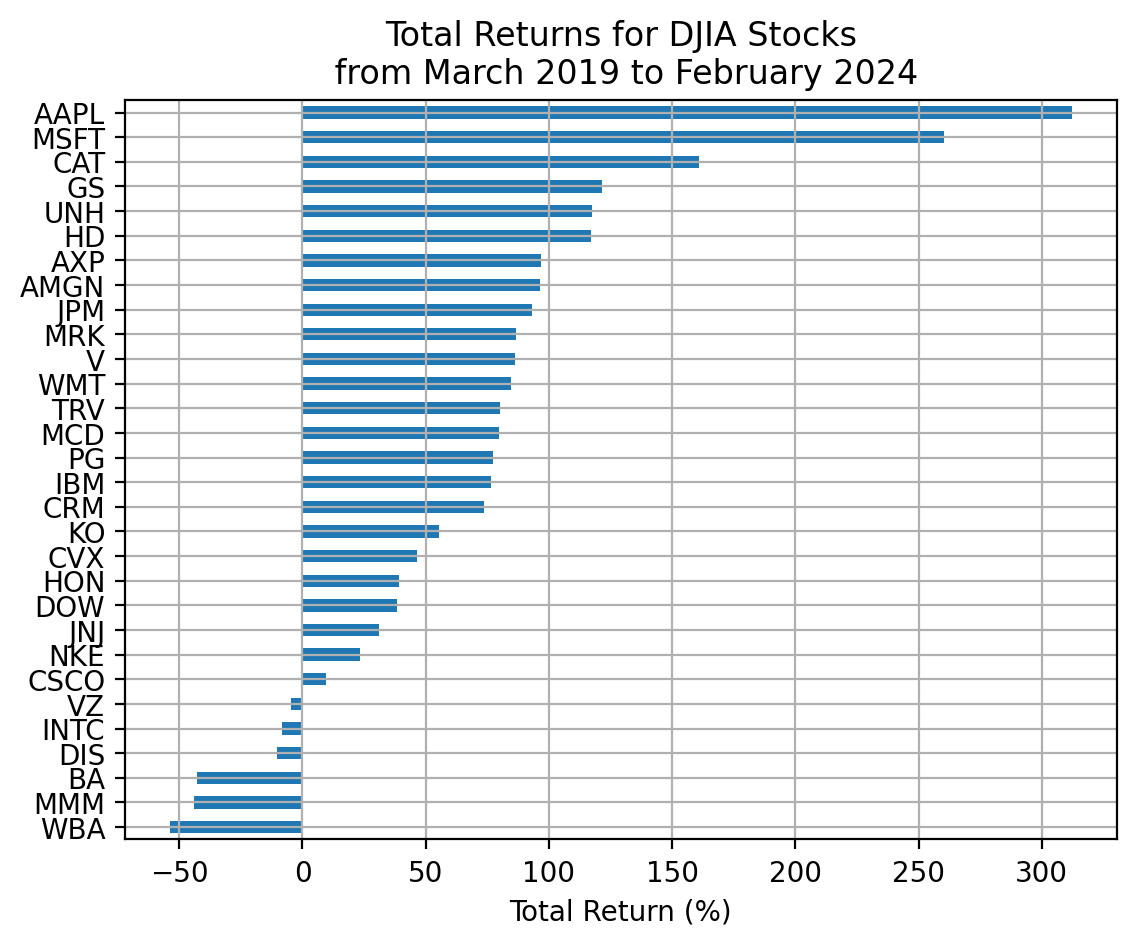
\includegraphics{mckinney_05_practice_04_files/figure-pdf/cell-25-output-1.png}

}

\end{figure}

\hypertarget{which-stocks-have-the-minimum-and-maximum-total-returns-2}{%
\subsection{Which stocks have the minimum and maximum total
returns?}\label{which-stocks-have-the-minimum-and-maximum-total-returns-2}}

If we want the \emph{values}, the \texttt{.min()} and \texttt{.max()}
methods are the way to go!

\begin{Shaded}
\begin{Highlighting}[]
\NormalTok{total\_returns2.}\BuiltInTok{min}\NormalTok{()}
\end{Highlighting}
\end{Shaded}

\begin{verbatim}
-0.5384
\end{verbatim}

\begin{Shaded}
\begin{Highlighting}[]
\NormalTok{total\_returns2.}\BuiltInTok{max}\NormalTok{()}
\end{Highlighting}
\end{Shaded}

\begin{verbatim}
3.1210
\end{verbatim}

The \texttt{.min()} and \texttt{.max()} methods give the values but not
the tickers (or index). We use the \texttt{.idxmin()} and
\texttt{.idxmax()} to get the tickers (or index).

\begin{Shaded}
\begin{Highlighting}[]
\NormalTok{total\_returns2.idxmin()}
\end{Highlighting}
\end{Shaded}

\begin{verbatim}
'WBA'
\end{verbatim}

\begin{Shaded}
\begin{Highlighting}[]
\NormalTok{total\_returns2.idxmax()}
\end{Highlighting}
\end{Shaded}

\begin{verbatim}
'AAPL'
\end{verbatim}

Here is what I would use!

\begin{Shaded}
\begin{Highlighting}[]
\NormalTok{total\_returns2.sort\_values().iloc[[}\DecValTok{0}\NormalTok{, }\OperatorTok{{-}}\DecValTok{1}\NormalTok{]]}
\end{Highlighting}
\end{Shaded}

\begin{verbatim}
WBA    -0.5384
AAPL    3.1210
dtype: float64
\end{verbatim}

Not the exactly right tool here, but the
\texttt{.nsmallest()\textquotesingle{}\ and}.nlargest()` methods are
really useful!

\begin{Shaded}
\begin{Highlighting}[]
\NormalTok{total\_returns2.nsmallest(}\DecValTok{3}\NormalTok{)}
\end{Highlighting}
\end{Shaded}

\begin{verbatim}
WBA   -0.5384
MMM   -0.4408
BA    -0.4289
dtype: float64
\end{verbatim}

\begin{Shaded}
\begin{Highlighting}[]
\NormalTok{total\_returns2.nlargest(}\DecValTok{3}\NormalTok{)}
\end{Highlighting}
\end{Shaded}

\begin{verbatim}
AAPL   3.1210
MSFT   2.6028
CAT    1.6083
dtype: float64
\end{verbatim}

\hypertarget{plot-the-cumulative-returns-for-the-stocks-in-the-djia-2}{%
\subsection{Plot the cumulative returns for the stocks in the
DJIA}\label{plot-the-cumulative-returns-for-the-stocks-in-the-djia-2}}

We can use the cumulative product method \texttt{.cumprod()} to
calculate the right hand side of the formula above.

\begin{Shaded}
\begin{Highlighting}[]
\NormalTok{start\_date }\OperatorTok{=}\NormalTok{ returns2.index.}\BuiltInTok{min}\NormalTok{()}
\NormalTok{stop\_date }\OperatorTok{=}\NormalTok{ returns2.index.}\BuiltInTok{max}\NormalTok{()}

\NormalTok{(}
\NormalTok{    returns2}
\NormalTok{    .add(}\DecValTok{1}\NormalTok{)}
\NormalTok{    .cumprod()}
\NormalTok{    .sub(}\DecValTok{1}\NormalTok{)}
\NormalTok{    .mul(}\DecValTok{100}\NormalTok{)}
\NormalTok{    .plot(legend}\OperatorTok{=}\VariableTok{False}\NormalTok{)}
\NormalTok{)}
\NormalTok{plt.ylabel(}\StringTok{\textquotesingle{}Cumulative Return (\%)\textquotesingle{}}\NormalTok{)}
\NormalTok{plt.title(}\SpecialStringTok{f\textquotesingle{}Cumulative Returns on DJIA Stocks}\CharTok{\textbackslash{}n}\SpecialStringTok{ from }\SpecialCharTok{\{}\NormalTok{start\_date}\SpecialCharTok{:}\OperatorTok{\%}\NormalTok{B }\OperatorTok{\%}\NormalTok{Y}\SpecialCharTok{\}}\SpecialStringTok{ to }\SpecialCharTok{\{}\NormalTok{stop\_date}\SpecialCharTok{:}\OperatorTok{\%}\NormalTok{B }\OperatorTok{\%}\NormalTok{Y}\SpecialCharTok{\}}\SpecialStringTok{\textquotesingle{}}\NormalTok{)}
\NormalTok{plt.show()}
\end{Highlighting}
\end{Shaded}

\begin{figure}[H]

{\centering 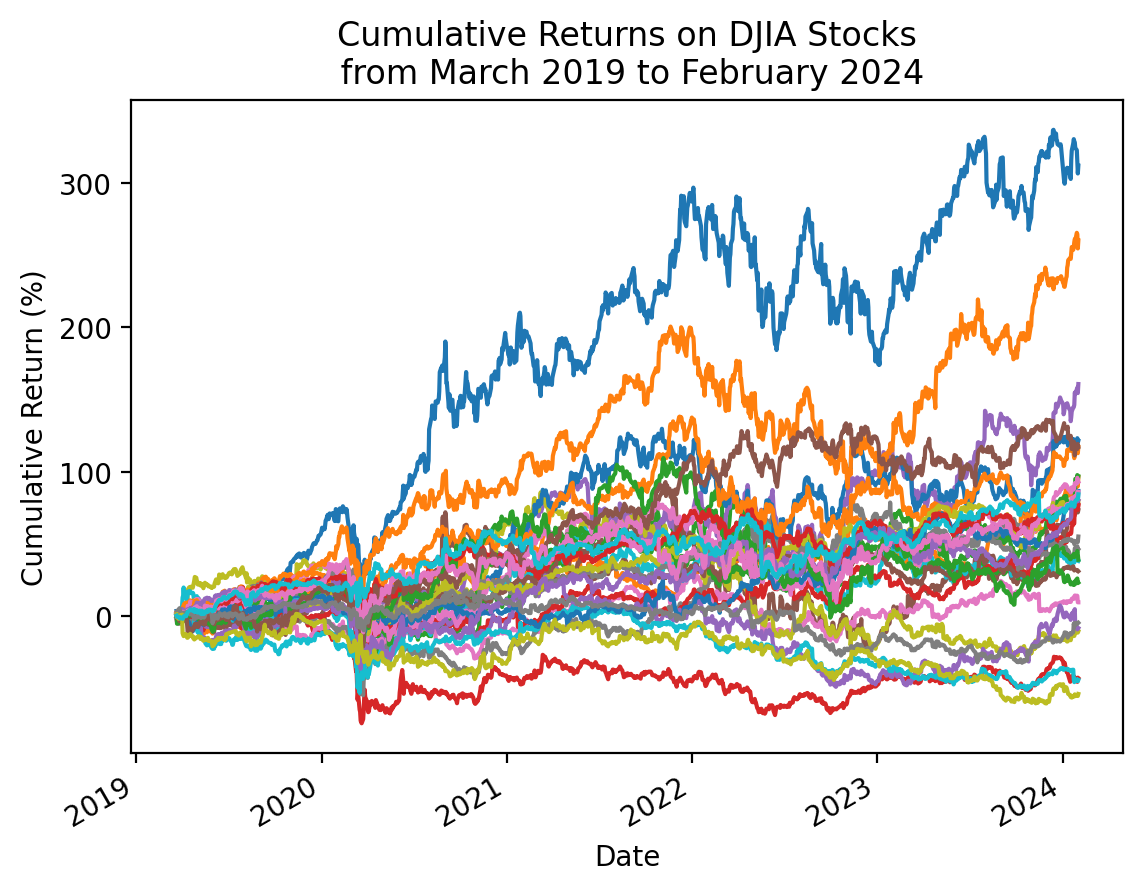
\includegraphics{mckinney_05_practice_04_files/figure-pdf/cell-33-output-1.png}

}

\end{figure}

\hypertarget{repeat-the-plot-above-with-only-the-minimum-and-maximum-total-returns-2}{%
\subsection{Repeat the plot above with only the minimum and maximum
total
returns}\label{repeat-the-plot-above-with-only-the-minimum-and-maximum-total-returns-2}}

\begin{Shaded}
\begin{Highlighting}[]
\NormalTok{total\_returns2.sort\_values().iloc[[}\DecValTok{0}\NormalTok{, }\OperatorTok{{-}}\DecValTok{1}\NormalTok{]].index}
\end{Highlighting}
\end{Shaded}

\begin{verbatim}
Index(['WBA', 'AAPL'], dtype='object')
\end{verbatim}

\begin{Shaded}
\begin{Highlighting}[]
\NormalTok{start\_date }\OperatorTok{=}\NormalTok{ returns2.index.}\BuiltInTok{min}\NormalTok{()}
\NormalTok{stop\_date }\OperatorTok{=}\NormalTok{ returns2.index.}\BuiltInTok{max}\NormalTok{()}

\NormalTok{(}
\NormalTok{    returns2[total\_returns2.sort\_values().iloc[[}\DecValTok{0}\NormalTok{, }\OperatorTok{{-}}\DecValTok{1}\NormalTok{]].index]}
\NormalTok{    .add(}\DecValTok{1}\NormalTok{)}
\NormalTok{    .cumprod()}
\NormalTok{    .sub(}\DecValTok{1}\NormalTok{)}
\NormalTok{    .mul(}\DecValTok{100}\NormalTok{)}
\NormalTok{    .plot()}
\NormalTok{)}
\NormalTok{plt.ylabel(}\StringTok{\textquotesingle{}Cumulative Return (\%)\textquotesingle{}}\NormalTok{)}
\NormalTok{plt.title(}\SpecialStringTok{f\textquotesingle{}Cumulative Returns on DJIA Stocks}\CharTok{\textbackslash{}n}\SpecialStringTok{ from }\SpecialCharTok{\{}\NormalTok{start\_date}\SpecialCharTok{:}\OperatorTok{\%}\NormalTok{B }\OperatorTok{\%}\NormalTok{Y}\SpecialCharTok{\}}\SpecialStringTok{ to }\SpecialCharTok{\{}\NormalTok{stop\_date}\SpecialCharTok{:}\OperatorTok{\%}\NormalTok{B }\OperatorTok{\%}\NormalTok{Y}\SpecialCharTok{\}}\SpecialStringTok{\textquotesingle{}}\NormalTok{)}
\NormalTok{plt.show()}
\end{Highlighting}
\end{Shaded}

\begin{figure}[H]

{\centering 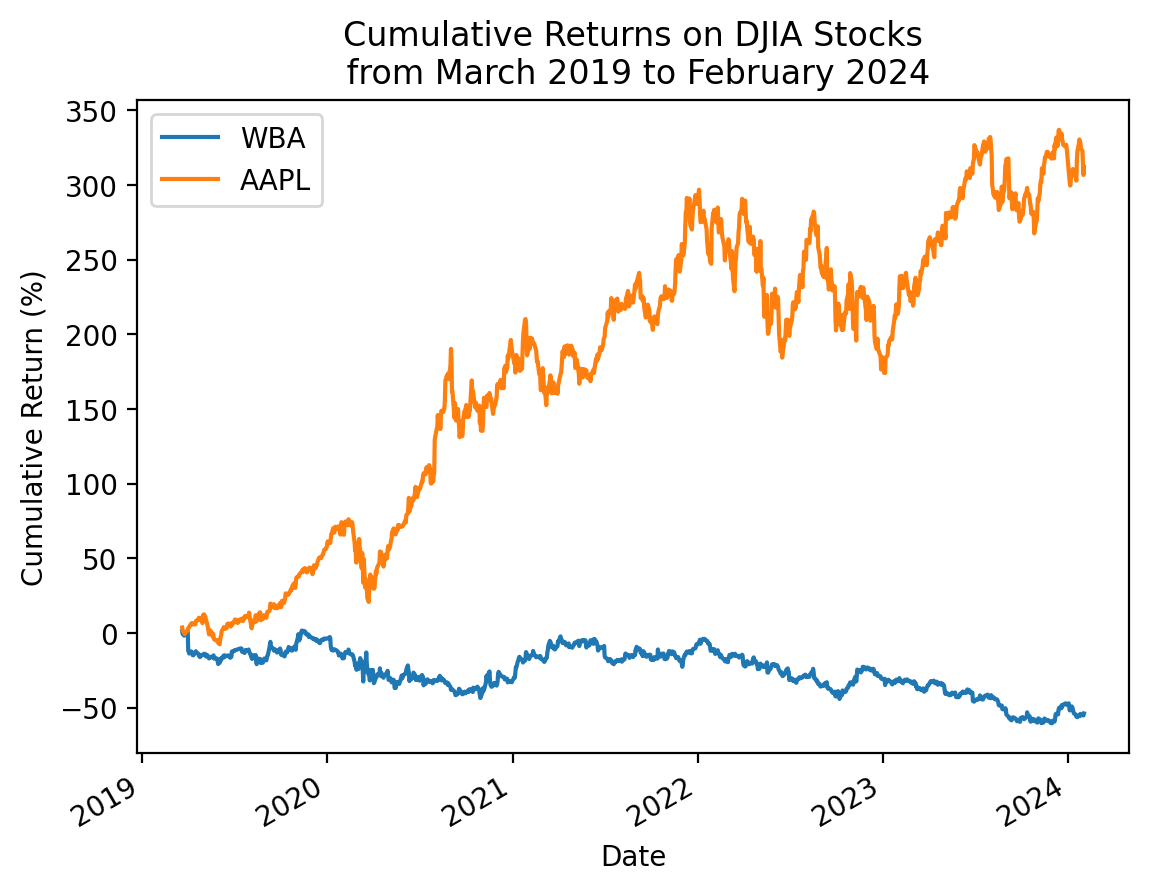
\includegraphics{mckinney_05_practice_04_files/figure-pdf/cell-35-output-1.png}

}

\end{figure}

\hypertarget{mckinney-chapter-5---practice-for-section-05}{%
\chapter{McKinney Chapter 5 - Practice for Section
05}\label{mckinney-chapter-5---practice-for-section-05}}

\hypertarget{announcements-15}{%
\section{Announcements}\label{announcements-15}}

\begin{enumerate}
\def\labelenumi{\arabic{enumi}.}
\tightlist
\item
  No DataCamp this week, but I suggest you keep working on it
\item
  Keep forming groups, and I will post our first project early next week
\end{enumerate}

\hypertarget{minute-recap-14}\NormalTok{precision }\DecValTok{4}
\NormalTok{pd.options.display.float\_format }\OperatorTok{=} \StringTok{\textquotesingle{}}\SpecialCharTok{\{:.4f\}}\StringTok{\textquotesingle{}}\NormalTok{.}\BuiltInTok{format}
\OperatorTok{\%}\NormalTok{config InlineBackend.figure\_format }\OperatorTok{=} \StringTok{\textquotesingle{}retina\textquotesingle{}}
\end{Highlighting}
\end{Shaded}

pandas gives us two data structures:

\begin{enumerate}
\def\labelenumi{\arabic{enumi}.}
\tightlist
\item
  Data Frames
\item
  Series
\end{enumerate}

A data frame is like a worksheet in an Excel workbook.

\begin{Shaded}
\begin{Highlighting}[]
\NormalTok{np.random.seed(}\DecValTok{42}\NormalTok{)}
\NormalTok{df }\OperatorTok{=}\NormalTok{ pd.DataFrame(}
\NormalTok{    data}\OperatorTok{=}\NormalTok{np.random.randn(}\DecValTok{3}\NormalTok{, }\DecValTok{5}\NormalTok{), }\CommentTok{\# 15 random numbers}
\NormalTok{    index}\OperatorTok{=}\BuiltInTok{list}\NormalTok{(}\StringTok{\textquotesingle{}ABC\textquotesingle{}}\NormalTok{), }\CommentTok{\# labels the rows for easy indexing and slicing}
\NormalTok{    columns}\OperatorTok{=}\BuiltInTok{list}\NormalTok{(}\StringTok{\textquotesingle{}abcde\textquotesingle{}}\NormalTok{) }\CommentTok{\# labels the columns for easy indexing and slicing}
\NormalTok{)}

\NormalTok{df}
\end{Highlighting}
\end{Shaded}

\begin{longtable}[]{@{}llllll@{}}
\toprule\noalign{}
& a & b & c & d & e \\
\midrule\noalign{}
\endhead
\bottomrule\noalign{}
\endlastfoot
A & 0.4967 & -0.1383 & 0.6477 & 1.5230 & -0.2342 \\
B & -0.2341 & 1.5792 & 0.7674 & -0.4695 & 0.5426 \\
C & -0.4634 & -0.4657 & 0.2420 & -1.9133 & -1.7249 \\
\end{longtable}

How can we get the first two rows and first three columns?

\begin{enumerate}
\def\labelenumi{\arabic{enumi}.}
\tightlist
\item
  We can slice by integer location with the \texttt{.iloc{[}{]}} method
\item
  We can slice by names with the \texttt{.loc{[}{]}} method
\end{enumerate}

\begin{Shaded}
\begin{Highlighting}[]
\NormalTok{df.iloc[:}\DecValTok{2}\NormalTok{, :}\DecValTok{3}\NormalTok{] }\CommentTok{\# j,k slicing, as in NumPy}
\end{Highlighting}
\end{Shaded}

\begin{longtable}[]{@{}llll@{}}
\toprule\noalign{}
& a & b & c \\
\midrule\noalign{}
\endhead
\bottomrule\noalign{}
\endlastfoot
A & 0.4967 & -0.1383 & 0.6477 \\
B & -0.2341 & 1.5792 & 0.7674 \\
\end{longtable}

\textbf{\emph{When we slice by names, both left and right edges are
}included\emph{!}}

\begin{Shaded}
\begin{Highlighting}[]
\NormalTok{df.loc[}\StringTok{\textquotesingle{}A\textquotesingle{}}\NormalTok{:}\StringTok{\textquotesingle{}B\textquotesingle{}}\NormalTok{, }\StringTok{\textquotesingle{}a\textquotesingle{}}\NormalTok{:}\StringTok{\textquotesingle{}c\textquotesingle{}}\NormalTok{]}
\end{Highlighting}
\end{Shaded}

\begin{longtable}[]{@{}llll@{}}
\toprule\noalign{}
& a & b & c \\
\midrule\noalign{}
\endhead
\bottomrule\noalign{}
\endlastfoot
A & 0.4967 & -0.1383 & 0.6477 \\
B & -0.2341 & 1.5792 & 0.7674 \\
\end{longtable}

We can use the \texttt{.head()} method to show the first \texttt{n} rows
in \texttt{df}.

\begin{Shaded}
\begin{Highlighting}[]
\NormalTok{df.head(}\DecValTok{2}\NormalTok{)}
\end{Highlighting}
\end{Shaded}

\begin{longtable}[]{@{}llllll@{}}
\toprule\noalign{}
& a & b & c & d & e \\
\midrule\noalign{}
\endhead
\bottomrule\noalign{}
\endlastfoot
A & 0.4967 & -0.1383 & 0.6477 & 1.5230 & -0.2342 \\
B & -0.2341 & 1.5792 & 0.7674 & -0.4695 & 0.5426 \\
\end{longtable}

How do I add a column?

\begin{Shaded}
\begin{Highlighting}[]
\NormalTok{df[}\StringTok{\textquotesingle{}f\textquotesingle{}}\NormalTok{] }\OperatorTok{=} \DecValTok{5} \CommentTok{\# as in NumPy, this 5 will broadcast to all the rows}

\NormalTok{df}
\end{Highlighting}
\end{Shaded}

\begin{longtable}[]{@{}lllllll@{}}
\toprule\noalign{}
& a & b & c & d & e & f \\
\midrule\noalign{}
\endhead
\bottomrule\noalign{}
\endlastfoot
A & 0.4967 & -0.1383 & 0.6477 & 1.5230 & -0.2342 & 5 \\
B & -0.2341 & 1.5792 & 0.7674 & -0.4695 & 0.5426 & 5 \\
C & -0.4634 & -0.4657 & 0.2420 & -1.9133 & -1.7249 & 5 \\
\end{longtable}

A series is like a single column in an Excel worksheet (or a pandas data
frame).

\begin{Shaded}
\begin{Highlighting}[]
\NormalTok{ser }\OperatorTok{=}\NormalTok{ pd.Series(data}\OperatorTok{=}\NormalTok{np.arange(}\FloatTok{2.}\NormalTok{), index}\OperatorTok{=}\BuiltInTok{list}\NormalTok{(}\StringTok{\textquotesingle{}BC\textquotesingle{}}\NormalTok{))}

\NormalTok{ser}
\end{Highlighting}
\end{Shaded}

\begin{verbatim}
B   0.0000
C   1.0000
dtype: float64
\end{verbatim}

pandas aligns operations on row and column names

\begin{Shaded}
\begin{Highlighting}[]
\NormalTok{df[}\StringTok{\textquotesingle{}g\textquotesingle{}}\NormalTok{] }\OperatorTok{=}\NormalTok{ ser}

\NormalTok{df}
\end{Highlighting}
\end{Shaded}

\begin{longtable}[]{@{}llllllll@{}}
\toprule\noalign{}
& a & b & c & d & e & f & g \\
\midrule\noalign{}
\endhead
\bottomrule\noalign{}
\endlastfoot
A & 0.4967 & -0.1383 & 0.6477 & 1.5230 & -0.2342 & 5 & NaN \\
B & -0.2341 & 1.5792 & 0.7674 & -0.4695 & 0.5426 & 5 & 0.0000 \\
C & -0.4634 & -0.4657 & 0.2420 & -1.9133 & -1.7249 & 5 & 1.0000 \\
\end{longtable}

\hypertarget{practice-15}{%
\section{Practice}\label{practice-15}}

\begin{Shaded}
\begin{Highlighting}[]
\NormalTok{tickers }\OperatorTok{=} \StringTok{\textquotesingle{}AAPL IBM MSFT GOOG\textquotesingle{}}
\NormalTok{prices }\OperatorTok{=}\NormalTok{ yf.download(tickers}\OperatorTok{=}\NormalTok{tickers)}
\end{Highlighting}
\end{Shaded}

\begin{verbatim}
[*********************100%%**********************]  4 of 4 completed
\end{verbatim}

\begin{Shaded}
\begin{Highlighting}[]
\NormalTok{returns }\OperatorTok{=}\NormalTok{ (}
\NormalTok{    prices[}\StringTok{\textquotesingle{}Adj Close\textquotesingle{}}\NormalTok{] }\CommentTok{\# slice adj close column}
\NormalTok{    .iloc[:}\OperatorTok{{-}}\DecValTok{1}\NormalTok{] }\CommentTok{\# drop last row with intra day prices, which are sometimes missing}
\NormalTok{    .pct\_change() }\CommentTok{\# calculate returns}
\NormalTok{    .dropna() }\CommentTok{\# drop leading rows with at least one missing value}
\NormalTok{)}

\NormalTok{returns}
\end{Highlighting}
\end{Shaded}

\begin{longtable}[]{@{}lllll@{}}
\toprule\noalign{}
& AAPL & GOOG & IBM & MSFT \\
Date & & & & \\
\midrule\noalign{}
\endhead
\bottomrule\noalign{}
\endlastfoot
2004-08-20 & 0.0029 & 0.0794 & 0.0042 & 0.0029 \\
2004-08-23 & 0.0091 & 0.0101 & -0.0070 & 0.0044 \\
2004-08-24 & 0.0280 & -0.0414 & 0.0007 & 0.0000 \\
2004-08-25 & 0.0344 & 0.0108 & 0.0042 & 0.0114 \\
2004-08-26 & 0.0487 & 0.0180 & -0.0045 & -0.0040 \\
... & ... & ... & ... & ... \\
2024-01-26 & -0.0090 & 0.0010 & -0.0158 & -0.0023 \\
2024-01-29 & -0.0036 & 0.0068 & -0.0015 & 0.0143 \\
2024-01-30 & -0.0192 & -0.0116 & 0.0039 & -0.0028 \\
2024-01-31 & -0.0194 & -0.0735 & -0.0224 & -0.0269 \\
2024-02-01 & 0.0133 & 0.0064 & 0.0176 & 0.0156 \\
\end{longtable}

\hypertarget{what-are-the-mean-daily-returns-for-these-four-stocks-3}{%
\subsection{What are the mean daily returns for these four
stocks?}\label{what-are-the-mean-daily-returns-for-these-four-stocks-3}}

\begin{Shaded}
\begin{Highlighting}[]
\NormalTok{returns.mean() }\CommentTok{\# default is axis=0, so we get the mean of each column}
\end{Highlighting}
\end{Shaded}

\begin{verbatim}
AAPL   0.0014
GOOG   0.0010
IBM    0.0004
MSFT   0.0008
dtype: float64
\end{verbatim}

We if want an equally-weighted portfolio return? We could take the mean
of each \emph{row} with \texttt{.mean(axis=1)}. The mean is the same as
the sum of 0.25 times each of the 4 columns.

\begin{Shaded}
\begin{Highlighting}[]
\NormalTok{returns.mean(axis}\OperatorTok{=}\DecValTok{1}\NormalTok{)}
\end{Highlighting}
\end{Shaded}

\begin{verbatim}
Date
2004-08-20    0.0224
2004-08-23    0.0041
2004-08-24   -0.0032
2004-08-25    0.0152
2004-08-26    0.0146
               ...  
2024-01-26   -0.0065
2024-01-29    0.0040
2024-01-30   -0.0074
2024-01-31   -0.0356
2024-02-01    0.0132
Length: 4896, dtype: float64
\end{verbatim}

\hypertarget{what-are-the-standard-deviations-of-daily-returns-for-these-four-stocks-3}{%
\subsection{What are the standard deviations of daily returns for these
four
stocks?}\label{what-are-the-standard-deviations-of-daily-returns-for-these-four-stocks-3}}

We can use the \texttt{.std()} method to find the \emph{sample} standard
deviation of each column.

\begin{Shaded}
\begin{Highlighting}[]
\NormalTok{returns.std()}
\end{Highlighting}
\end{Shaded}

\begin{verbatim}
AAPL   0.0206
GOOG   0.0194
IBM    0.0143
MSFT   0.0171
dtype: float64
\end{verbatim}

\hypertarget{what-are-the-annualized-means-and-standard-deviations-of-daily-returns-for-these-four-stocks-3}{%
\subsection{\texorpdfstring{What are the \emph{annualized} means and
standard deviations of daily returns for these four
stocks?}{What are the annualized means and standard deviations of daily returns for these four stocks?}}\label{what-are-the-annualized-means-and-standard-deviations-of-daily-returns-for-these-four-stocks-3}}

We annualize mean returns by multiplying by \(T\) (\(T=252\) for daily
returns, \(T=12\) for month returns, and so on). We annualize standard
deviations by multiplying by \(\sqrt(T)\).

\begin{Shaded}
\begin{Highlighting}[]
\NormalTok{returns.mean().mul(}\DecValTok{252}\NormalTok{) }\CommentTok{\# whenever I can, I use the .mul() method, so I can keep chaining!}
\end{Highlighting}
\end{Shaded}

\begin{verbatim}
AAPL   0.3625
GOOG   0.2552
IBM    0.0980
MSFT   0.2002
dtype: float64
\end{verbatim}

\begin{Shaded}
\begin{Highlighting}[]
\NormalTok{returns.std().mul(np.sqrt(}\DecValTok{252}\NormalTok{))}
\end{Highlighting}
\end{Shaded}

\begin{verbatim}
AAPL   0.3276
GOOG   0.3074
IBM    0.2272
MSFT   0.2722
dtype: float64
\end{verbatim}

\hypertarget{plot-annualized-means-versus-standard-deviations-of-daily-returns-for-these-four-stocks-3}{%
\subsection{\texorpdfstring{Plot \emph{annualized} means versus standard
deviations of daily returns for these four
stocks}{Plot annualized means versus standard deviations of daily returns for these four stocks}}\label{plot-annualized-means-versus-standard-deviations-of-daily-returns-for-these-four-stocks-3}}

Use \texttt{plt.scatter()}, which expects arguments as \texttt{x}
(standard deviations) then \texttt{y} (means).

\begin{Shaded}
\begin{Highlighting}[]
\NormalTok{vols }\OperatorTok{=}\NormalTok{ returns.std().mul(np.sqrt(}\DecValTok{252}\NormalTok{) }\OperatorTok{*} \DecValTok{100}\NormalTok{)}
\NormalTok{means }\OperatorTok{=}\NormalTok{ returns.mean().mul(}\DecValTok{252} \OperatorTok{*} \DecValTok{100}\NormalTok{)}

\NormalTok{plt.scatter(}
\NormalTok{    x}\OperatorTok{=}\NormalTok{vols,}
\NormalTok{    y}\OperatorTok{=}\NormalTok{means}
\NormalTok{)}

\NormalTok{plt.xlabel(}\StringTok{\textquotesingle{}Annualized Volatility of Daily Returns (\%)\textquotesingle{}}\NormalTok{)}
\NormalTok{plt.ylabel(}\StringTok{\textquotesingle{}Annualized Mean of Daily Returns (\%)\textquotesingle{}}\NormalTok{)}

\CommentTok{\# plt.xlim((0, vols.max() + 5))}
\CommentTok{\# plt.ylim((0, means.max() + 5))}

\CommentTok{\# add tickers to each point}
\ControlFlowTok{for}\NormalTok{ i }\KeywordTok{in}\NormalTok{ means.index: }\CommentTok{\# loop over ticker index}
\NormalTok{    plt.text( }\CommentTok{\# plots string s at coordinates x and y}
\NormalTok{        x}\OperatorTok{=}\NormalTok{vols[i], }\CommentTok{\# indexes volatility}
\NormalTok{        y}\OperatorTok{=}\NormalTok{means[i], }\CommentTok{\# indexes mean return}
\NormalTok{        s}\OperatorTok{=}\NormalTok{i }\CommentTok{\# ticker index}
\NormalTok{    )}

\NormalTok{plt.title(}\StringTok{\textquotesingle{}Returns versus Risk\textquotesingle{}}\NormalTok{)}
\NormalTok{plt.show() }\CommentTok{\# suppresses output of last function call}
\end{Highlighting}
\end{Shaded}

\begin{figure}[H]

{\centering \includegraphics{mckinney_05_practice_05_files/figure-pdf/cell-18-output-1.png}

}

\end{figure}

\hypertarget{repeat-the-previous-calculations-and-plot-for-the-stocks-in-the-dow-jones-industrial-index-djia-3}{%
\subsection{Repeat the previous calculations and plot for the stocks in
the Dow-Jones Industrial Index
(DJIA)}\label{repeat-the-previous-calculations-and-plot-for-the-stocks-in-the-dow-jones-industrial-index-djia-3}}

We can find the current DJIA stocks on
\href{https://en.wikipedia.org/wiki/Dow_Jones_Industrial_Average}{Wikipedia}.
We will need to download new data, into \texttt{tickers2},
\texttt{prices2}, and \texttt{returns2}.

\begin{Shaded}
\begin{Highlighting}[]
\NormalTok{url2 }\OperatorTok{=} \StringTok{\textquotesingle{}https://en.wikipedia.org/wiki/Dow\_Jones\_Industrial\_Average\textquotesingle{}}
\NormalTok{wiki2 }\OperatorTok{=}\NormalTok{ pd.read\_html(io}\OperatorTok{=}\NormalTok{url2)}
\NormalTok{tickers2 }\OperatorTok{=}\NormalTok{ wiki2[}\DecValTok{1}\NormalTok{][}\StringTok{\textquotesingle{}Symbol\textquotesingle{}}\NormalTok{].to\_list()}
\NormalTok{tickers2[:}\DecValTok{5}\NormalTok{]}
\end{Highlighting}
\end{Shaded}

\begin{verbatim}
['MMM', 'AXP', 'AMGN', 'AAPL', 'BA']
\end{verbatim}

\begin{Shaded}
\begin{Highlighting}[]
\NormalTok{prices2 }\OperatorTok{=}\NormalTok{ yf.download(tickers}\OperatorTok{=}\NormalTok{tickers2)}
\end{Highlighting}
\end{Shaded}

\begin{verbatim}
[*********************100%%**********************]  30 of 30 completed
\end{verbatim}

\begin{Shaded}
\begin{Highlighting}[]
\NormalTok{returns2 }\OperatorTok{=}\NormalTok{ (}
\NormalTok{    prices2[}\StringTok{\textquotesingle{}Adj Close\textquotesingle{}}\NormalTok{] }\CommentTok{\# slices the adj close group of columns from prices}
\NormalTok{    .iloc[:}\OperatorTok{{-}}\DecValTok{1}\NormalTok{] }\CommentTok{\# drop last row (which is intraday during class) to avoid fill\_method warning}
\NormalTok{    .pct\_change() }\CommentTok{\# calculate percent in adj closes (row[n] {-} row[n{-}1]) / row[n{-}1]}
\NormalTok{    .dropna() }\CommentTok{\# drops rows with any missing values}
\NormalTok{)}

\NormalTok{returns2}
\end{Highlighting}
\end{Shaded}

\begin{longtable}[]{@{}llllllllllllllllllllll@{}}
\toprule\noalign{}
& AAPL & AMGN & AXP & BA & CAT & CRM & CSCO & CVX & DIS & DOW & ... &
MRK & MSFT & NKE & PG & TRV & UNH & V & VZ & WBA & WMT \\
Date & & & & & & & & & & & & & & & & & & & & & \\
\midrule\noalign{}
\endhead
\bottomrule\noalign{}
\endlastfoot
2019-03-21 & 0.0368 & 0.0040 & 0.0095 & -0.0092 & 0.0079 & 0.0210 &
0.0128 & 0.0094 & -0.0121 & -0.0165 & ... & 0.0106 & 0.0230 & 0.0152 &
0.0076 & 0.0231 & 0.0061 & 0.0133 & 0.0108 & 0.0129 & 0.0043 \\
2019-03-22 & -0.0207 & -0.0270 & -0.0211 & -0.0283 & -0.0320 & -0.0326 &
-0.0222 & -0.0220 & -0.0040 & -0.0078 & ... & -0.0080 & -0.0264 &
-0.0661 & -0.0081 & 0.0039 & -0.0196 & -0.0175 & 0.0252 & -0.0187 &
-0.0079 \\
2019-03-25 & -0.0121 & -0.0006 & -0.0038 & 0.0229 & 0.0124 & -0.0038 &
-0.0002 & -0.0016 & -0.0041 & 0.0113 & ... & 0.0007 & 0.0052 & 0.0017 &
0.0030 & 0.0004 & -0.0009 & -0.0003 & 0.0054 & -0.0115 & -0.0011 \\
2019-03-26 & -0.0103 & 0.0090 & 0.0042 & -0.0002 & 0.0035 & -0.0092 &
0.0095 & 0.0101 & 0.0218 & -0.0061 & ... & 0.0069 & 0.0021 & 0.0128 &
0.0104 & 0.0002 & -0.0141 & 0.0148 & 0.0092 & 0.0037 & 0.0015 \\
2019-03-27 & 0.0090 & -0.0104 & -0.0047 & 0.0103 & -0.0049 & -0.0269 &
-0.0017 & -0.0108 & 0.0013 & 0.0256 & ... & -0.0076 & -0.0097 & -0.0035
& -0.0012 & 0.0101 & -0.0069 & -0.0070 & 0.0041 & 0.0050 & -0.0113 \\
... & ... & ... & ... & ... & ... & ... & ... & ... & ... & ... & ... &
... & ... & ... & ... & ... & ... & ... & ... & ... & ... \\
2024-01-26 & -0.0090 & 0.0049 & 0.0710 & 0.0178 & -0.0045 & 0.0033 &
-0.0036 & 0.0038 & 0.0053 & -0.0160 & ... & 0.0057 & -0.0023 & 0.0196 &
0.0033 & -0.0004 & 0.0199 & -0.0171 & 0.0026 & -0.0113 & 0.0088 \\
2024-01-29 & -0.0036 & 0.0054 & -0.0028 & -0.0014 & 0.0128 & 0.0283 &
0.0029 & -0.0004 & 0.0223 & 0.0002 & ... & 0.0038 & 0.0143 & 0.0110 &
0.0001 & -0.0015 & 0.0027 & 0.0213 & -0.0083 & -0.0057 & 0.0047 \\
2024-01-30 & -0.0192 & 0.0037 & 0.0164 & -0.0231 & 0.0050 & -0.0005 &
-0.0010 & 0.0070 & -0.0056 & 0.0074 & ... & 0.0031 & -0.0028 & 0.0029 &
0.0085 & 0.0115 & -0.0018 & 0.0128 & 0.0100 & 0.0018 & 0.0033 \\
2024-01-31 & -0.0194 & -0.0011 & -0.0167 & 0.0529 & -0.0146 & -0.0231 &
-0.0394 & -0.0179 & -0.0092 & -0.0160 & ... & -0.0072 & -0.0269 &
-0.0254 & -0.0022 & -0.0102 & 0.0161 & -0.0140 & -0.0028 & -0.0083 &
-0.0021 \\
2024-02-01 & 0.0133 & 0.0328 & 0.0124 & -0.0058 & 0.0246 & 0.0096 &
0.0000 & 0.0031 & 0.0105 & -0.0011 & ... & 0.0464 & 0.0156 & 0.0023 &
0.0130 & 0.0031 & -0.0090 & 0.0139 & 0.0033 & 0.0301 & 0.0185 \\
\end{longtable}

\begin{Shaded}
\begin{Highlighting}[]
\NormalTok{vols }\OperatorTok{=}\NormalTok{ returns2.std().mul(np.sqrt(}\DecValTok{252}\NormalTok{) }\OperatorTok{*} \DecValTok{100}\NormalTok{)}
\NormalTok{means }\OperatorTok{=}\NormalTok{ returns2.mean().mul(}\DecValTok{252} \OperatorTok{*} \DecValTok{100}\NormalTok{)}

\NormalTok{plt.scatter(}
\NormalTok{    x}\OperatorTok{=}\NormalTok{vols,}
\NormalTok{    y}\OperatorTok{=}\NormalTok{means}
\NormalTok{)}

\NormalTok{plt.xlabel(}\StringTok{\textquotesingle{}Annualized Volatility of Daily Returns (\%)\textquotesingle{}}\NormalTok{)}
\NormalTok{plt.ylabel(}\StringTok{\textquotesingle{}Annualized Mean of Daily Returns (\%)\textquotesingle{}}\NormalTok{)}

\CommentTok{\# plt.xlim((0, vols.max() + 5))}
\CommentTok{\# plt.ylim((0, means.max() + 5))}

\CommentTok{\# add tickers to each point}
\ControlFlowTok{for}\NormalTok{ i }\KeywordTok{in}\NormalTok{ means.index: }\CommentTok{\# loop over ticker index}
\NormalTok{    plt.text( }\CommentTok{\# plots string s at coordinates x and y}
\NormalTok{        x}\OperatorTok{=}\NormalTok{vols[i], }\CommentTok{\# indexes volatility}
\NormalTok{        y}\OperatorTok{=}\NormalTok{means[i], }\CommentTok{\# indexes mean return}
\NormalTok{        s}\OperatorTok{=}\NormalTok{i }\CommentTok{\# ticker index}
\NormalTok{    )}

\NormalTok{plt.title(}\StringTok{\textquotesingle{}Returns versus Risk\textquotesingle{}}\NormalTok{)}
\NormalTok{plt.show() }\CommentTok{\# suppresses output of last function call}
\end{Highlighting}
\end{Shaded}

\begin{figure}[H]

{\centering \includegraphics{mckinney_05_practice_05_files/figure-pdf/cell-22-output-1.png}

}

\end{figure}

With 30 stocks we see there is no relation between returns and
volatility because most volatility is \emph{diversifiable} and
uncompensated.

\hypertarget{calculate-total-returns-for-the-stocks-in-the-djia-3}{%
\subsection{Calculate total returns for the stocks in the
DJIA}\label{calculate-total-returns-for-the-stocks-in-the-djia-3}}

We can use the \texttt{.prod()} method to compound returns as
\(1 + R_T = \prod_{t=1}^T (1 + R_t)\). Technically, we should write
\(R_T\) as \(R_{0,T}\), but we typically omit the subscript \(0\).

In general, I prefer to do simple math on pandas objects (data frames
and series) with methods instead of operators:

For example:

\begin{enumerate}
\def\labelenumi{\arabic{enumi}.}
\tightlist
\item
  \texttt{.add(1)} instead of \texttt{+\ 1}
\item
  \texttt{.sub(1)} instead of \texttt{-\ 1}
\item
  \texttt{.div(1)} instead of \texttt{/\ 1}
\item
  \texttt{.mul(1)} instead of \texttt{*\ 1}
\end{enumerate}

The advantage of methods over operators, is that we can easily chain
methods without lots of parentheses.

\begin{Shaded}
\begin{Highlighting}[]
\NormalTok{total\_returns2 }\OperatorTok{=}\NormalTok{ returns2.add(}\DecValTok{1}\NormalTok{).prod().sub(}\DecValTok{1}\NormalTok{)}

\NormalTok{total\_returns2.iloc[:}\DecValTok{5}\NormalTok{]}
\end{Highlighting}
\end{Shaded}

\begin{verbatim}
AAPL    3.1210
AMGN    0.9635
AXP     0.9687
BA     -0.4289
CAT     1.6083
dtype: float64
\end{verbatim}

\hypertarget{plot-the-distribution-of-total-returns-for-the-stocks-in-the-djia-3}{%
\subsection{Plot the distribution of total returns for the stocks in the
DJIA}\label{plot-the-distribution-of-total-returns-for-the-stocks-in-the-djia-3}}

We can plot a histogram, using either the \texttt{plt.hist()} function
or the \texttt{.plot(kind=\textquotesingle{}hist\textquotesingle{})}
method.

A histogram is a great way to visualize data!

\begin{Shaded}
\begin{Highlighting}[]
\NormalTok{start\_date }\OperatorTok{=}\NormalTok{ returns2.index.}\BuiltInTok{min}\NormalTok{()}
\NormalTok{stop\_date }\OperatorTok{=}\NormalTok{ returns2.index.}\BuiltInTok{max}\NormalTok{()}

\NormalTok{(}
\NormalTok{    returns2}
\NormalTok{    .add(}\DecValTok{1}\NormalTok{)}
\NormalTok{    .prod()}
\NormalTok{    .sub(}\DecValTok{1}\NormalTok{)}
\NormalTok{    .mul(}\DecValTok{100}\NormalTok{)}
\NormalTok{    .plot(kind}\OperatorTok{=}\StringTok{\textquotesingle{}hist\textquotesingle{}}\NormalTok{, bins}\OperatorTok{=}\DecValTok{20}\NormalTok{) }\CommentTok{\# grids=True to add grid lines}
\NormalTok{)}
\NormalTok{plt.xlabel(}\StringTok{\textquotesingle{}Total Return (\%)\textquotesingle{}}\NormalTok{)}
\NormalTok{plt.title(}\SpecialStringTok{f\textquotesingle{}Distribution of Total Returns for DJIA Stocks}\CharTok{\textbackslash{}n}\SpecialStringTok{ from }\SpecialCharTok{\{}\NormalTok{start\_date}\SpecialCharTok{:}\OperatorTok{\%}\NormalTok{B }\OperatorTok{\%}\NormalTok{Y}\SpecialCharTok{\}}\SpecialStringTok{ to }\SpecialCharTok{\{}\NormalTok{stop\_date}\SpecialCharTok{:}\OperatorTok{\%}\NormalTok{B }\OperatorTok{\%}\NormalTok{Y}\SpecialCharTok{\}}\SpecialStringTok{\textquotesingle{}}\NormalTok{)}
\NormalTok{plt.show()}
\end{Highlighting}
\end{Shaded}

\begin{figure}[H]

{\centering \includegraphics{mckinney_05_practice_05_files/figure-pdf/cell-24-output-1.png}

}

\end{figure}

With only 30 stocks, we can actually connect a stock to its return in a
plot!

\begin{Shaded}
\begin{Highlighting}[]
\NormalTok{start\_date }\OperatorTok{=}\NormalTok{ returns2.index.}\BuiltInTok{min}\NormalTok{()}
\NormalTok{stop\_date }\OperatorTok{=}\NormalTok{ returns2.index.}\BuiltInTok{max}\NormalTok{()}

\NormalTok{(}
\NormalTok{    returns2}
\NormalTok{    .add(}\DecValTok{1}\NormalTok{)}
\NormalTok{    .prod()}
\NormalTok{    .sub(}\DecValTok{1}\NormalTok{)}
\NormalTok{    .sort\_values() }\CommentTok{\# sort by total returns}
\NormalTok{    .mul(}\DecValTok{100}\NormalTok{)}
\NormalTok{    .plot(kind}\OperatorTok{=}\StringTok{\textquotesingle{}barh\textquotesingle{}}\NormalTok{) }\CommentTok{\# horizontal bar chart}
\NormalTok{)}
\NormalTok{plt.xlabel(}\StringTok{\textquotesingle{}Total Return (\%)\textquotesingle{}}\NormalTok{)}
\NormalTok{plt.title(}\SpecialStringTok{f\textquotesingle{}Distribution of Total Returns for DJIA Stocks}\CharTok{\textbackslash{}n}\SpecialStringTok{ from }\SpecialCharTok{\{}\NormalTok{start\_date}\SpecialCharTok{:}\OperatorTok{\%}\NormalTok{B }\OperatorTok{\%}\NormalTok{Y}\SpecialCharTok{\}}\SpecialStringTok{ to }\SpecialCharTok{\{}\NormalTok{stop\_date}\SpecialCharTok{:}\OperatorTok{\%}\NormalTok{B }\OperatorTok{\%}\NormalTok{Y}\SpecialCharTok{\}}\SpecialStringTok{\textquotesingle{}}\NormalTok{)}
\NormalTok{plt.show()}
\end{Highlighting}
\end{Shaded}

\begin{figure}[H]

{\centering 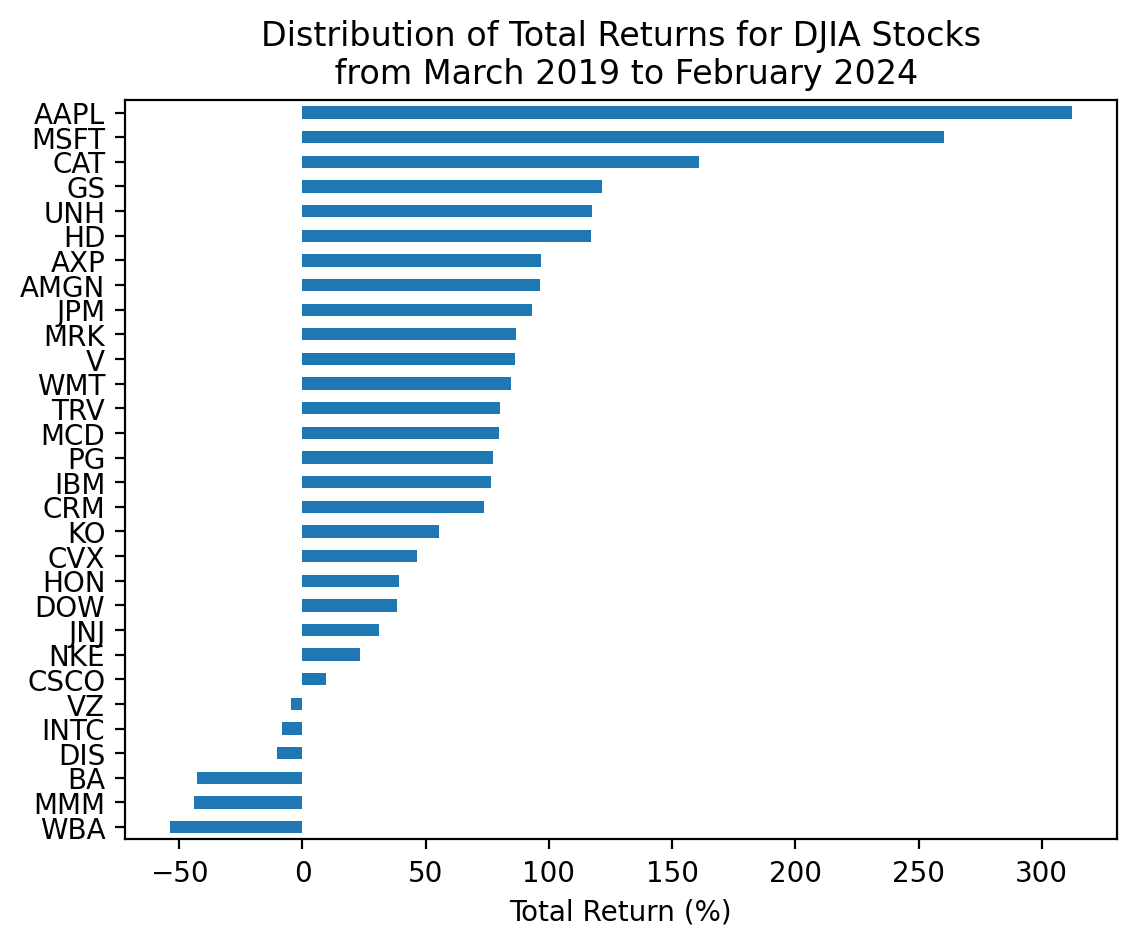
\includegraphics{mckinney_05_practice_05_files/figure-pdf/cell-25-output-1.png}

}

\end{figure}

\hypertarget{which-stocks-have-the-minimum-and-maximum-total-returns-3}{%
\subsection{Which stocks have the minimum and maximum total
returns?}\label{which-stocks-have-the-minimum-and-maximum-total-returns-3}}

If we want the \emph{values}, the \texttt{.min()} and \texttt{.max()}
methods are the way to go!

\begin{Shaded}
\begin{Highlighting}[]
\NormalTok{total\_returns2.}\BuiltInTok{min}\NormalTok{()}
\end{Highlighting}
\end{Shaded}

\begin{verbatim}
-0.5384
\end{verbatim}

\begin{Shaded}
\begin{Highlighting}[]
\NormalTok{total\_returns2.}\BuiltInTok{max}\NormalTok{()}
\end{Highlighting}
\end{Shaded}

\begin{verbatim}
3.1210
\end{verbatim}

The \texttt{.min()} and \texttt{.max()} methods give the values but not
the tickers (or index). We use the \texttt{.idxmin()} and
\texttt{.idxmax()} to get the tickers (or index).

\begin{Shaded}
\begin{Highlighting}[]
\NormalTok{total\_returns2.idxmin()}
\end{Highlighting}
\end{Shaded}

\begin{verbatim}
'WBA'
\end{verbatim}

\begin{Shaded}
\begin{Highlighting}[]
\NormalTok{total\_returns2.idxmax()}
\end{Highlighting}
\end{Shaded}

\begin{verbatim}
'AAPL'
\end{verbatim}

Here is what I would use!

\begin{Shaded}
\begin{Highlighting}[]
\NormalTok{total\_returns2.sort\_values().iloc[[}\DecValTok{0}\NormalTok{, }\OperatorTok{{-}}\DecValTok{1}\NormalTok{]]}
\end{Highlighting}
\end{Shaded}

\begin{verbatim}
WBA    -0.5384
AAPL    3.1210
dtype: float64
\end{verbatim}

Not the exactly right tool here, but the
\texttt{.nsmallest()\textquotesingle{}\ and}.nlargest()` methods are
really useful!

\begin{Shaded}
\begin{Highlighting}[]
\NormalTok{total\_returns2.nsmallest(}\DecValTok{3}\NormalTok{)}
\end{Highlighting}
\end{Shaded}

\begin{verbatim}
WBA   -0.5384
MMM   -0.4408
BA    -0.4289
dtype: float64
\end{verbatim}

\begin{Shaded}
\begin{Highlighting}[]
\NormalTok{total\_returns2.nlargest(}\DecValTok{3}\NormalTok{)}
\end{Highlighting}
\end{Shaded}

\begin{verbatim}
AAPL   3.1210
MSFT   2.6028
CAT    1.6083
dtype: float64
\end{verbatim}

\hypertarget{plot-the-cumulative-returns-for-the-stocks-in-the-djia-3}{%
\subsection{Plot the cumulative returns for the stocks in the
DJIA}\label{plot-the-cumulative-returns-for-the-stocks-in-the-djia-3}}

We can use the cumulative product method \texttt{.cumprod()} to
calculate the right hand side of the formula above.

\begin{Shaded}
\begin{Highlighting}[]
\NormalTok{start\_date }\OperatorTok{=}\NormalTok{ returns2.index.}\BuiltInTok{min}\NormalTok{()}
\NormalTok{stop\_date }\OperatorTok{=}\NormalTok{ returns2.index.}\BuiltInTok{max}\NormalTok{()}

\NormalTok{(}
\NormalTok{    returns2}
\NormalTok{    .add(}\DecValTok{1}\NormalTok{)}
\NormalTok{    .cumprod()}
\NormalTok{    .sub(}\DecValTok{1}\NormalTok{)}
\NormalTok{    .mul(}\DecValTok{100}\NormalTok{)}
\NormalTok{    .plot(legend}\OperatorTok{=}\VariableTok{False}\NormalTok{) }\CommentTok{\# with 30 stocks, this legend is too big to be useful}
\NormalTok{)}

\NormalTok{plt.ylabel(}\StringTok{\textquotesingle{}Cumulative Return (\%)\textquotesingle{}}\NormalTok{)}
\NormalTok{plt.title(}\SpecialStringTok{f\textquotesingle{}Cumulative Returns for DJIA Stocks}\CharTok{\textbackslash{}n}\SpecialStringTok{ from }\SpecialCharTok{\{}\NormalTok{start\_date}\SpecialCharTok{:}\OperatorTok{\%}\NormalTok{B }\OperatorTok{\%}\NormalTok{Y}\SpecialCharTok{\}}\SpecialStringTok{ to }\SpecialCharTok{\{}\NormalTok{stop\_date}\SpecialCharTok{:}\OperatorTok{\%}\NormalTok{B }\OperatorTok{\%}\NormalTok{Y}\SpecialCharTok{\}}\SpecialStringTok{\textquotesingle{}}\NormalTok{)}
\NormalTok{plt.show()}
\end{Highlighting}
\end{Shaded}

\begin{figure}[H]

{\centering 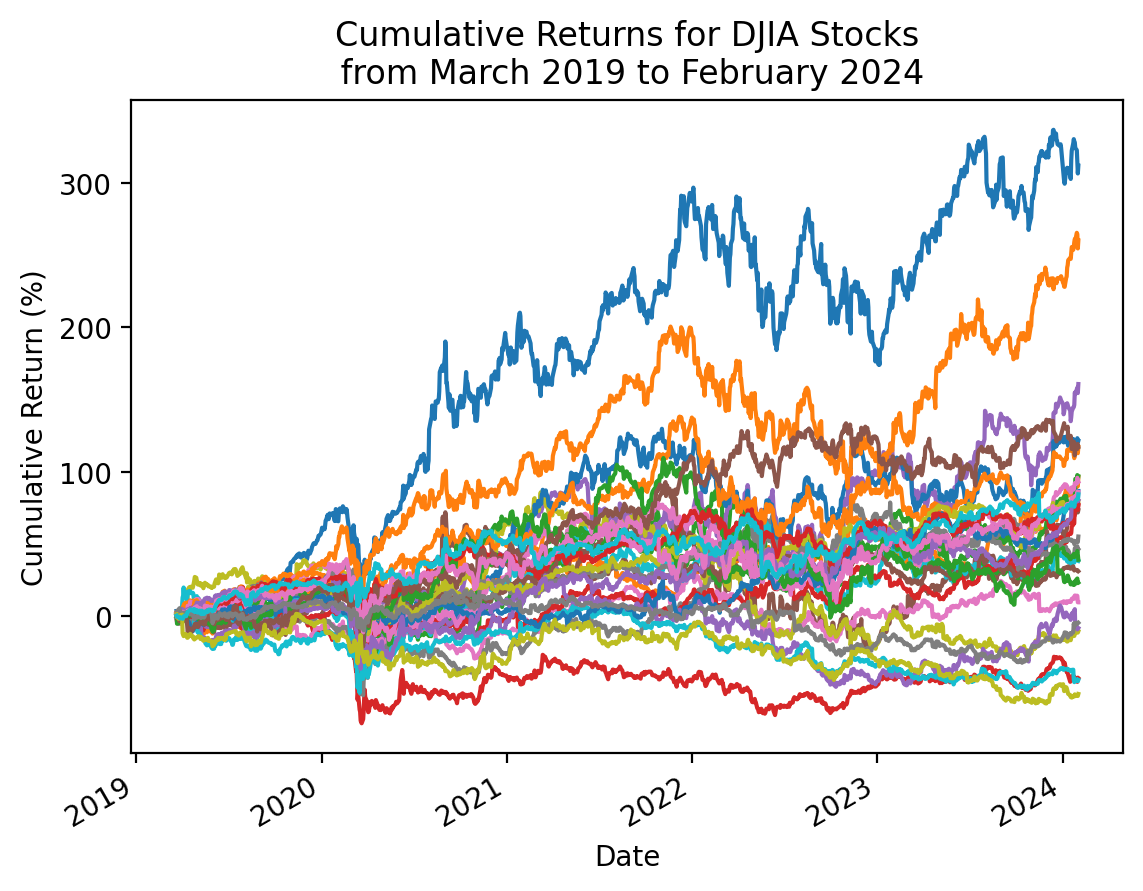
\includegraphics{mckinney_05_practice_05_files/figure-pdf/cell-33-output-1.png}

}

\end{figure}

\hypertarget{repeat-the-plot-above-with-only-the-minimum-and-maximum-total-returns-3}{%
\subsection{Repeat the plot above with only the minimum and maximum
total
returns}\label{repeat-the-plot-above-with-only-the-minimum-and-maximum-total-returns-3}}

\begin{Shaded}
\begin{Highlighting}[]
\NormalTok{total\_returns2.sort\_values().iloc[[}\DecValTok{0}\NormalTok{, }\OperatorTok{{-}}\DecValTok{1}\NormalTok{]].index}
\end{Highlighting}
\end{Shaded}

\begin{verbatim}
Index(['WBA', 'AAPL'], dtype='object')
\end{verbatim}

\begin{Shaded}
\begin{Highlighting}[]
\NormalTok{returns2[total\_returns2.sort\_values().iloc[[}\DecValTok{0}\NormalTok{, }\OperatorTok{{-}}\DecValTok{1}\NormalTok{]].index]}
\end{Highlighting}
\end{Shaded}

\begin{longtable}[]{@{}lll@{}}
\toprule\noalign{}
& WBA & AAPL \\
Date & & \\
\midrule\noalign{}
\endhead
\bottomrule\noalign{}
\endlastfoot
2019-03-21 & 0.0129 & 0.0368 \\
2019-03-22 & -0.0187 & -0.0207 \\
2019-03-25 & -0.0115 & -0.0121 \\
2019-03-26 & 0.0037 & -0.0103 \\
2019-03-27 & 0.0050 & 0.0090 \\
... & ... & ... \\
2024-01-26 & -0.0113 & -0.0090 \\
2024-01-29 & -0.0057 & -0.0036 \\
2024-01-30 & 0.0018 & -0.0192 \\
2024-01-31 & -0.0083 & -0.0194 \\
2024-02-01 & 0.0301 & 0.0133 \\
\end{longtable}

\begin{Shaded}
\begin{Highlighting}[]
\NormalTok{start\_date }\OperatorTok{=}\NormalTok{ returns2.index.}\BuiltInTok{min}\NormalTok{()}
\NormalTok{stop\_date }\OperatorTok{=}\NormalTok{ returns2.index.}\BuiltInTok{max}\NormalTok{()}

\NormalTok{(}
\NormalTok{    returns2 }\CommentTok{\# all returns for all stocks}
\NormalTok{    [total\_returns2.sort\_values().iloc[[}\DecValTok{0}\NormalTok{, }\OperatorTok{{-}}\DecValTok{1}\NormalTok{]].index] }\CommentTok{\# slice min and max total return stocks}
\NormalTok{    .add(}\DecValTok{1}\NormalTok{)}
\NormalTok{    .cumprod()}
\NormalTok{    .sub(}\DecValTok{1}\NormalTok{)}
\NormalTok{    .mul(}\DecValTok{100}\NormalTok{)}
\NormalTok{    .plot()}
\NormalTok{)}
\NormalTok{plt.ylabel(}\StringTok{\textquotesingle{}Cumulative Return (\%)\textquotesingle{}}\NormalTok{)}
\NormalTok{plt.title(}\SpecialStringTok{f\textquotesingle{}Cumulative Returns for DJIA Stocks}\CharTok{\textbackslash{}n}\SpecialStringTok{ from }\SpecialCharTok{\{}\NormalTok{start\_date}\SpecialCharTok{:}\OperatorTok{\%}\NormalTok{B }\OperatorTok{\%}\NormalTok{Y}\SpecialCharTok{\}}\SpecialStringTok{ to }\SpecialCharTok{\{}\NormalTok{stop\_date}\SpecialCharTok{:}\OperatorTok{\%}\NormalTok{B }\OperatorTok{\%}\NormalTok{Y}\SpecialCharTok{\}}\SpecialStringTok{\textquotesingle{}}\NormalTok{)}
\NormalTok{plt.show()}
\end{Highlighting}
\end{Shaded}

\begin{figure}[H]

{\centering 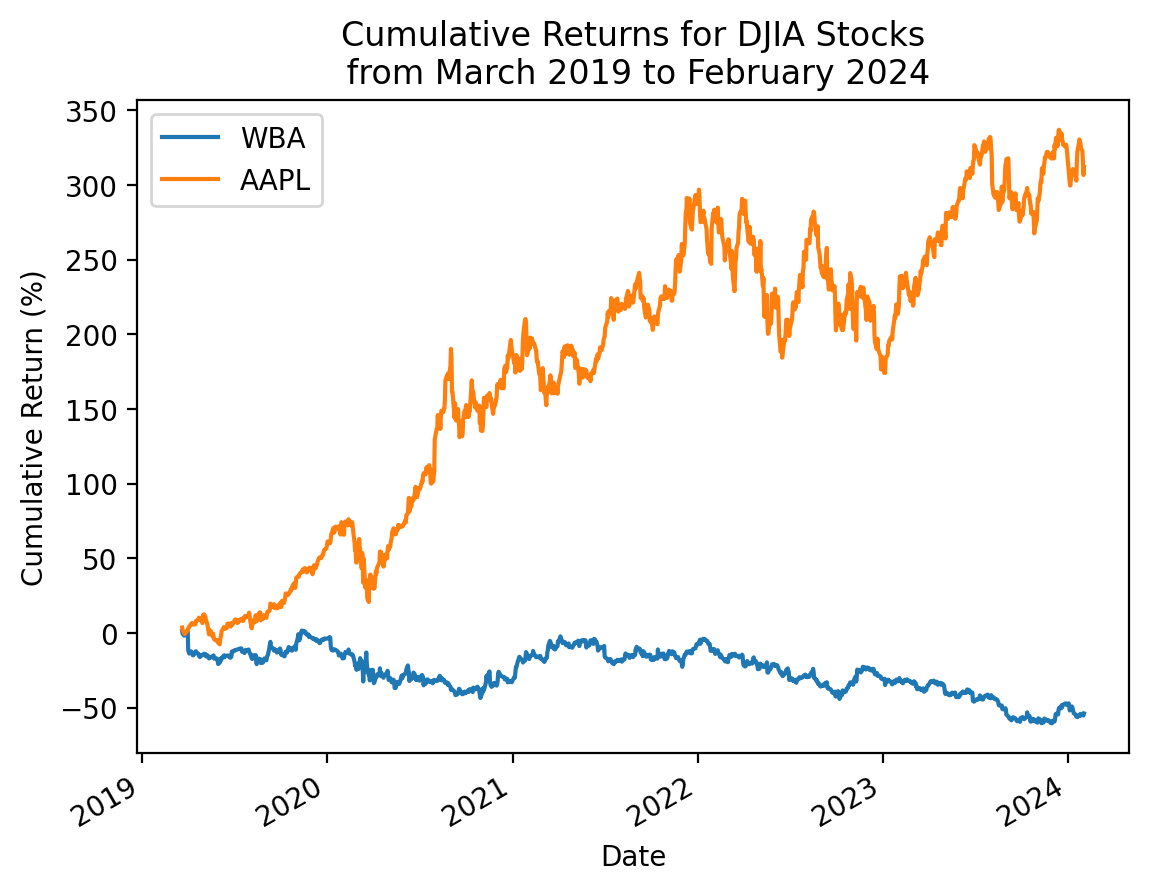
\includegraphics{mckinney_05_practice_05_files/figure-pdf/cell-36-output-1.png}

}

\end{figure}

\part{Week 5}

\hypertarget{herron-topic-1---web-data-log-and-simple-returns-and-portfolio-math}{%
\chapter{Herron Topic 1 - Web Data, Log and Simple Returns, and
Portfolio
Math}\label{herron-topic-1---web-data-log-and-simple-returns-and-portfolio-math}}

This notebook covers three topics:

\begin{enumerate}
\def\labelenumi{\arabic{enumi}.}
\tightlist
\item
  How to download web data with the yfinance and pandas-datareader
  packages
\item
  How to calculate log and simple returns
\item
  How to calculate portfolio returns
\end{enumerate}

\begin{Shaded}
\begin{Highlighting}[]
\ImportTok{import}\NormalTok{ matplotlib.pyplot }\ImportTok{as}\NormalTok{ plt}
\ImportTok{import}\NormalTok{ numpy }\ImportTok{as}\NormalTok{ np}
\ImportTok{import}\NormalTok{ pandas }\ImportTok{as}\NormalTok{ pd}
\end{Highlighting}
\end{Shaded}

\begin{Shaded}
\begin{Highlighting}[]
\OperatorTok{\%}\NormalTok{precision }\DecValTok{4}
\NormalTok{pd.options.display.float\_format }\OperatorTok{=} \StringTok{\textquotesingle{}}\SpecialCharTok{\{:.4f\}}\StringTok{\textquotesingle{}}\NormalTok{.}\BuiltInTok{format}
\OperatorTok{\%}\NormalTok{config InlineBackend.figure\_format }\OperatorTok{=} \StringTok{\textquotesingle{}retina\textquotesingle{}}
\end{Highlighting}
\end{Shaded}

\hypertarget{web-data}{%
\section{Web Data}\label{web-data}}

We will typically use the yfinance and pandas-datarader packages to
download data from the web. If you followed my instructions to install
Miniconda on your computer, you have already installed these packages.

\hypertarget{the-yfinance-package}{%
\subsection{The yfinance Package}\label{the-yfinance-package}}

The \href{https://github.com/ranaroussi/yfinance}{yfinance package}
provides ``a reliable, threaded, and Pythonic way to download historical
market data from Yahoo! finance.'' Other packages provide similar
functionality, but yfinance is best.

\begin{Shaded}
\begin{Highlighting}[]
\ImportTok{import}\NormalTok{ yfinance }\ImportTok{as}\NormalTok{ yf}
\end{Highlighting}
\end{Shaded}

We can download data for the MATANA stocks (Microsoft, Alphabet, Tesla,
Amazon, Nvidia, and Apple). We can pass tickers as either a
space-delimited string or a list of strings.

\begin{Shaded}
\begin{Highlighting}[]
\NormalTok{df }\OperatorTok{=}\NormalTok{ yf.download(tickers}\OperatorTok{=}\StringTok{\textquotesingle{}MSFT GOOG TSLA AMZN NVDA AAPL\textquotesingle{}}\NormalTok{)}
\NormalTok{df}
\end{Highlighting}
\end{Shaded}

\begin{verbatim}
[*********************100%%**********************]  6 of 6 completed
\end{verbatim}

\begin{longtable}[]{@{}llllllllllllllllllllll@{}}
\toprule\noalign{}
&
\multicolumn{6}{>{\raggedright\arraybackslash}p{(\columnwidth - 42\tabcolsep) * \real{0.0000} + 10\tabcolsep}}{%
Adj Close} &
\multicolumn{4}{>{\raggedright\arraybackslash}p{(\columnwidth - 42\tabcolsep) * \real{0.0000} + 6\tabcolsep}}{%
Close} & ... &
\multicolumn{4}{>{\raggedright\arraybackslash}p{(\columnwidth - 42\tabcolsep) * \real{0.0000} + 6\tabcolsep}}{%
Open} &
\multicolumn{6}{>{\raggedright\arraybackslash}p{(\columnwidth - 42\tabcolsep) * \real{0.0000} + 10\tabcolsep}@{}}{%
Volume} \\
& AAPL & AMZN & GOOG & MSFT & NVDA & TSLA & AAPL & AMZN & GOOG & MSFT &
... & GOOG & MSFT & NVDA & TSLA & AAPL & AMZN & GOOG & MSFT & NVDA &
TSLA \\
Date & & & & & & & & & & & & & & & & & & & & & \\
\midrule\noalign{}
\endhead
\bottomrule\noalign{}
\endlastfoot
1980-12-12 & 0.0993 & NaN & NaN & NaN & NaN & NaN & 0.1283 & NaN & NaN &
NaN & ... & NaN & NaN & NaN & NaN & 469033600 & NaN & NaN & NaN & NaN &
NaN \\
1980-12-15 & 0.0941 & NaN & NaN & NaN & NaN & NaN & 0.1217 & NaN & NaN &
NaN & ... & NaN & NaN & NaN & NaN & 175884800 & NaN & NaN & NaN & NaN &
NaN \\
1980-12-16 & 0.0872 & NaN & NaN & NaN & NaN & NaN & 0.1127 & NaN & NaN &
NaN & ... & NaN & NaN & NaN & NaN & 105728000 & NaN & NaN & NaN & NaN &
NaN \\
1980-12-17 & 0.0894 & NaN & NaN & NaN & NaN & NaN & 0.1155 & NaN & NaN &
NaN & ... & NaN & NaN & NaN & NaN & 86441600 & NaN & NaN & NaN & NaN &
NaN \\
1980-12-18 & 0.0920 & NaN & NaN & NaN & NaN & NaN & 0.1189 & NaN & NaN &
NaN & ... & NaN & NaN & NaN & NaN & 73449600 & NaN & NaN & NaN & NaN &
NaN \\
... & ... & ... & ... & ... & ... & ... & ... & ... & ... & ... & ... &
... & ... & ... & ... & ... & ... & ... & ... & ... & ... \\
2024-01-26 & 192.4200 & 159.1200 & 153.7900 & 403.9300 & 610.3100 &
183.2500 & 192.4200 & 159.1200 & 153.7900 & 403.9300 & ... & 152.8700 &
404.3700 & 609.6000 & 185.5000 & 44553400 & 51001100.0000 &
19483600.0000 & 17786700.0000 & 38983800.0000 & 107063400.0000 \\
2024-01-29 & 191.7300 & 161.2600 & 154.8400 & 409.7200 & 624.6500 &
190.9300 & 191.7300 & 161.2600 & 154.8400 & 409.7200 & ... & 153.6400 &
406.0600 & 612.3200 & 185.6300 & 47145600 & 45270400.0000 &
20909300.0000 & 24510200.0000 & 34873300.0000 & 125013100.0000 \\
2024-01-30 & 188.0400 & 159.0000 & 153.0500 & 408.5900 & 627.7400 &
191.5900 & 188.0400 & 159.0000 & 153.0500 & 408.5900 & ... & 154.0100 &
412.2600 & 629.0000 & 195.3300 & 55859400 & 45207400.0000 &
26578900.0000 & 33477600.0000 & 41073500.0000 & 109982300.0000 \\
2024-01-31 & 184.4000 & 155.2000 & 141.8000 & 397.5800 & 615.2700 &
187.2900 & 184.4000 & 155.2000 & 141.8000 & 397.5800 & ... & 145.3900 &
406.9600 & 614.4000 & 187.0000 & 55467800 & 50284400.0000 &
43908600.0000 & 47871100.0000 & 45379500.0000 & 103221400.0000 \\
2024-02-01 & 186.8600 & 159.2800 & 142.7100 & 403.7800 & 630.2700 &
188.8600 & 186.8600 & 159.2800 & 142.7100 & 403.7800 & ... & 143.6900 &
401.8300 & 621.0000 & 188.5000 & 52672619 & 63406285.0000 &
24997783.0000 & 29155588.0000 & 35818376.0000 & 90546003.0000 \\
\end{longtable}

\begin{Shaded}
\begin{Highlighting}[]
\NormalTok{(}
\NormalTok{    df}
\NormalTok{    [}\StringTok{\textquotesingle{}Adj Close\textquotesingle{}}\NormalTok{]}
\NormalTok{    .pct\_change()}
\NormalTok{    .loc[}\StringTok{\textquotesingle{}2023\textquotesingle{}}\NormalTok{]}
\NormalTok{    .add(}\DecValTok{1}\NormalTok{)}
\NormalTok{    .cumprod()}
\NormalTok{    .sub(}\DecValTok{1}\NormalTok{)}
\NormalTok{    .mul(}\DecValTok{100}\NormalTok{)}
\NormalTok{    .plot()}
\NormalTok{)}
\NormalTok{plt.ylabel(}\StringTok{\textquotesingle{}Year{-}to{-}Date Return (\%)\textquotesingle{}}\NormalTok{)}
\NormalTok{plt.title(}\StringTok{\textquotesingle{}Year{-}to{-}Date Returns for MATANA Stocks in 2023\textquotesingle{}}\NormalTok{)}
\NormalTok{plt.show()}
\end{Highlighting}
\end{Shaded}

\begin{figure}[H]

{\centering 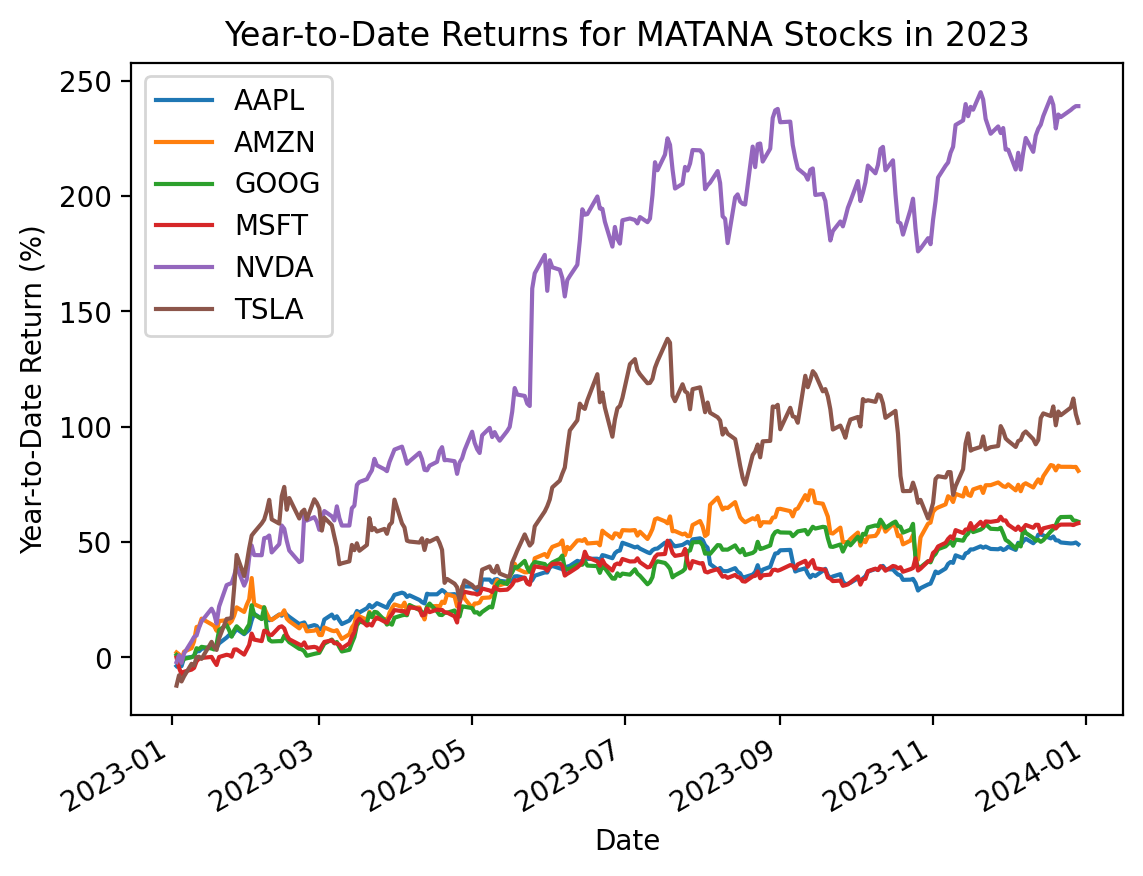
\includegraphics{herron_01_lecture_files/figure-pdf/cell-6-output-1.png}

}

\end{figure}

\hypertarget{the-pandas-datareader-package}{%
\subsection{The pandas-datareader
package}\label{the-pandas-datareader-package}}

The
\href{https://pandas-datareader.readthedocs.io/en/latest/index.html}{pandas-datareader}
package provides easy access to various data sources, including
\href{https://mba.tuck.dartmouth.edu/pages/faculty/ken.french/data_library.html}{the
Kenneth French Data Library} and \href{https://fred.stlouisfed.org/}{the
Federal Reserve Economic Data (FRED)}. The pandas-datareader package
also downloads Yahoo! Finance data, but the yfinance package has better
documentation. We will use \texttt{pdr} as the abbreviated prefix for
pandas-datareader.

\begin{Shaded}
\begin{Highlighting}[]
\ImportTok{import}\NormalTok{ pandas\_datareader }\ImportTok{as}\NormalTok{ pdr}
\end{Highlighting}
\end{Shaded}

Here we download the daily benchmark factors from Ken French's Data
Library.

\begin{Shaded}
\begin{Highlighting}[]
\NormalTok{pdr.famafrench.get\_available\_datasets()[:}\DecValTok{5}\NormalTok{]}
\end{Highlighting}
\end{Shaded}

\begin{verbatim}
['F-F_Research_Data_Factors',
 'F-F_Research_Data_Factors_weekly',
 'F-F_Research_Data_Factors_daily',
 'F-F_Research_Data_5_Factors_2x3',
 'F-F_Research_Data_5_Factors_2x3_daily']
\end{verbatim}

For Fama and French data, pandas-datareader returns the most recent five
years of data unless we specify a \texttt{start} date. French typically
provides data back through the second half of 1926. pandas-datareader
returns dictionaries of data frames, and the
\texttt{\textquotesingle{}DESCR\textquotesingle{}} value describes these
data frames.

\begin{Shaded}
\begin{Highlighting}[]
\NormalTok{ff\_all }\OperatorTok{=}\NormalTok{ pdr.DataReader(}
\NormalTok{    name}\OperatorTok{=}\StringTok{\textquotesingle{}F{-}F\_Research\_Data\_Factors\_daily\textquotesingle{}}\NormalTok{,}
\NormalTok{    data\_source}\OperatorTok{=}\StringTok{\textquotesingle{}famafrench\textquotesingle{}}\NormalTok{,}
\NormalTok{    start}\OperatorTok{=}\StringTok{\textquotesingle{}1900\textquotesingle{}}
\NormalTok{)}
\end{Highlighting}
\end{Shaded}

\begin{verbatim}
C:\Users\r.herron\AppData\Local\Temp\ipykernel_26796\2526882917.py:1: FutureWarning: The argument 'date_parser' is deprecated and will be removed in a future version. Please use 'date_format' instead, or read your data in as 'object' dtype and then call 'to_datetime'.
  ff_all = pdr.DataReader(
\end{verbatim}

\begin{Shaded}
\begin{Highlighting}[]
\BuiltInTok{type}\NormalTok{(ff\_all)}
\end{Highlighting}
\end{Shaded}

\begin{verbatim}
dict
\end{verbatim}

\begin{Shaded}
\begin{Highlighting}[]
\BuiltInTok{print}\NormalTok{(ff\_all[}\StringTok{\textquotesingle{}DESCR\textquotesingle{}}\NormalTok{])}
\end{Highlighting}
\end{Shaded}

\begin{verbatim}
F-F Research Data Factors daily
-------------------------------

This file was created by CMPT_ME_BEME_RETS_DAILY using the 202312 CRSP database. The Tbill return is the simple daily rate that, over the number of trading days in the month, compounds to 1-month TBill rate from Ibbotson and Associates Inc. Copyright 2023 Kenneth R. French

  0 : (25649 rows x 4 cols)
\end{verbatim}

\begin{Shaded}
\begin{Highlighting}[]
\NormalTok{ff\_all[}\DecValTok{0}\NormalTok{]}
\end{Highlighting}
\end{Shaded}

\begin{longtable}[]{@{}lllll@{}}
\toprule\noalign{}
& Mkt-RF & SMB & HML & RF \\
Date & & & & \\
\midrule\noalign{}
\endhead
\bottomrule\noalign{}
\endlastfoot
1926-07-01 & 0.1000 & -0.2500 & -0.2700 & 0.0090 \\
1926-07-02 & 0.4500 & -0.3300 & -0.0600 & 0.0090 \\
1926-07-06 & 0.1700 & 0.3000 & -0.3900 & 0.0090 \\
1926-07-07 & 0.0900 & -0.5800 & 0.0200 & 0.0090 \\
1926-07-08 & 0.2100 & -0.3800 & 0.1900 & 0.0090 \\
... & ... & ... & ... & ... \\
2023-12-22 & 0.2100 & 0.6400 & 0.0900 & 0.0210 \\
2023-12-26 & 0.4800 & 0.6900 & 0.4600 & 0.0210 \\
2023-12-27 & 0.1600 & 0.1400 & 0.1200 & 0.0210 \\
2023-12-28 & -0.0100 & -0.3600 & 0.0300 & 0.0210 \\
2023-12-29 & -0.4300 & -1.1200 & -0.3700 & 0.0210 \\
\end{longtable}

\begin{Shaded}
\begin{Highlighting}[]
\NormalTok{(}
\NormalTok{    ff\_all[}\DecValTok{0}\NormalTok{] }\CommentTok{\# slice factors}
\NormalTok{    .div(}\DecValTok{100}\NormalTok{) }\CommentTok{\# convert to decimal}
\NormalTok{    .add(}\DecValTok{1}\NormalTok{) }\CommentTok{\# calculate cumulative returns}
\NormalTok{    .cumprod()}
\NormalTok{    .sub(}\DecValTok{1}\NormalTok{)}
\NormalTok{    .mul(}\DecValTok{100}\NormalTok{) }\CommentTok{\# convert to percent}
\NormalTok{    .plot() }\CommentTok{\# plot}
\NormalTok{)}
\NormalTok{plt.ylabel(}\StringTok{\textquotesingle{}Cumulative Return (\%)\textquotesingle{}}\NormalTok{)}
\NormalTok{plt.title(}\StringTok{\textquotesingle{}Cumulative Returns for the Daily Benchmark Factors\textquotesingle{}}\NormalTok{)}
\NormalTok{plt.gca().yaxis.set\_major\_formatter(plt.matplotlib.ticker.StrMethodFormatter(}\StringTok{\textquotesingle{}\{x:,.0f\}\textquotesingle{}}\NormalTok{))}
\CommentTok{\# plt.yscale(\textquotesingle{}log\textquotesingle{}) \# log scale impractical here with negative returns}
\NormalTok{plt.show()}
\end{Highlighting}
\end{Shaded}

\begin{figure}[H]

{\centering 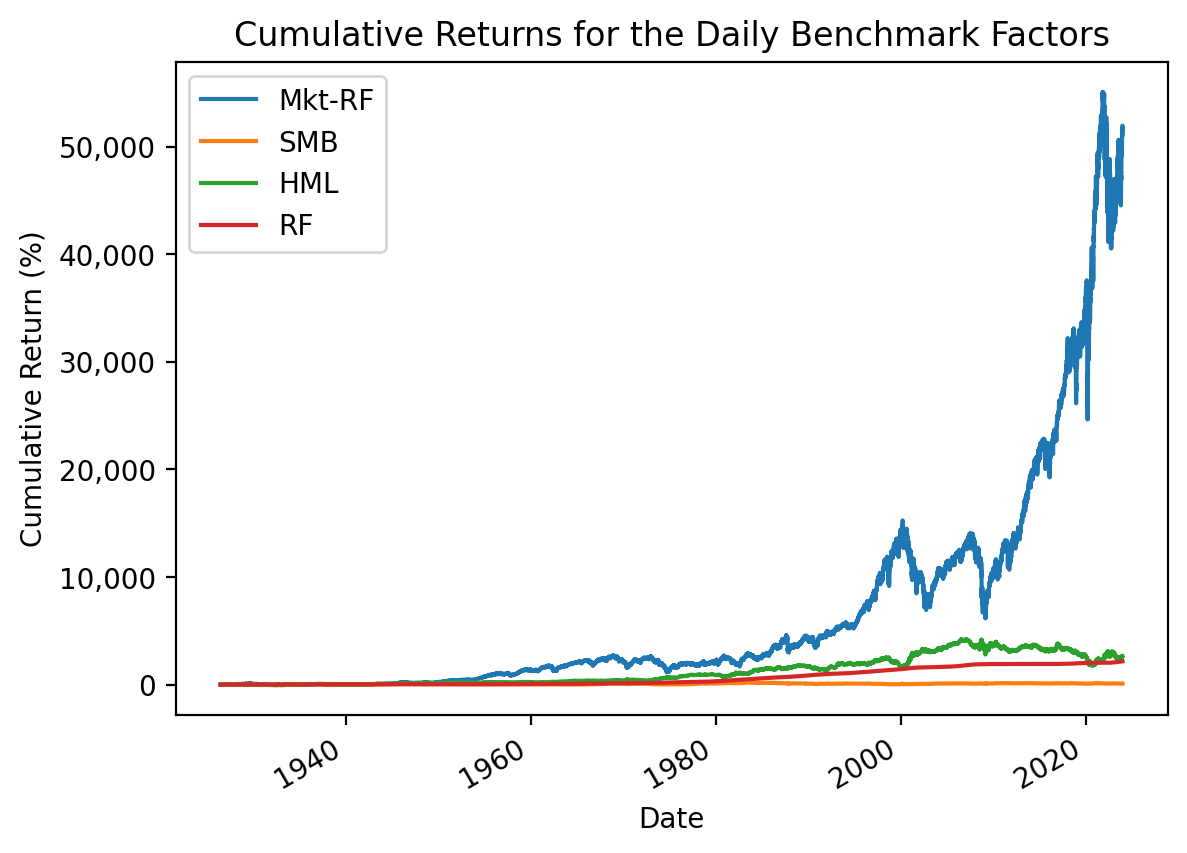
\includegraphics{herron_01_lecture_files/figure-pdf/cell-13-output-1.png}

}

\end{figure}

\hypertarget{log-and-simple-returns}{%
\section{Log and Simple Returns}\label{log-and-simple-returns}}

We will typically use \emph{simple} returns, calculated as
\(R_{simple,t} = \frac{P_t + D_t - P_{t-1}}{P_{t-1}} = \frac{P_t + D_t}{P_{t-1}} - 1\).
The simple return is the return that investors receive on invested
dollars. We can calculate simple returns from Yahoo Finance data with
the \texttt{.pct\_change()} method on the adjusted close column (i.e.,
\texttt{Adj\ Close}), which adjusts for dividends and splits. The
adjusted close column is a reverse-engineered close price (i.e.,
end-of-trading-day price) that incorporates dividends and splits, making
simple return calculations easy.

However, we may see \emph{log} returns elsewhere, which are the
(natural) log of one plus simple returns:
\[R_{log,t} = \log(1 + R_{simple,t}) = \log\left(1 +  \frac{P_t + D_t}{P_{t-1}} - 1 \right) = \log\left(\frac{P_t + D_t}{P_{t-1}} \right) = \log(P_t + D_t) - \log(P_{t-1})\]
Therefore, we calculate log returns as either the log of one plus simple
returns or the difference of the logs of the adjusted close column. Log
returns are also known as \emph{continuously-compounded} returns.

We will typically use \emph{simple} returns instead of \emph{log}
returns. However, this section explains the differences between simple
and log returns and where each is appropriate.

\hypertarget{simple-and-log-returns-are-similar-for-small-returns}{%
\subsection{Simple and Log Returns are Similar for Small
Returns}\label{simple-and-log-returns-are-similar-for-small-returns}}

\(\log(1 + x) \approx x\) for small values of \(x\), so simple returns
and log returns are similar for small returns. Returns are typically
small at daily and monthly horizons, so the difference between simple
and log returns is small at these horizons. The following figure shows
\(R_{simple,t} \approx R_{log,t}\) for small \(R\)s.

\begin{Shaded}
\begin{Highlighting}[]
\NormalTok{R }\OperatorTok{=}\NormalTok{ np.linspace(}\OperatorTok{{-}}\FloatTok{0.75}\NormalTok{, }\FloatTok{0.75}\NormalTok{, }\DecValTok{100}\NormalTok{)}
\NormalTok{logR }\OperatorTok{=}\NormalTok{ np.log(}\DecValTok{1} \OperatorTok{+}\NormalTok{ R)}
\end{Highlighting}
\end{Shaded}

\begin{Shaded}
\begin{Highlighting}[]
\NormalTok{plt.plot(R, logR)}
\NormalTok{plt.plot([}\OperatorTok{{-}}\DecValTok{1}\NormalTok{, }\DecValTok{1}\NormalTok{], [}\OperatorTok{{-}}\DecValTok{1}\NormalTok{, }\DecValTok{1}\NormalTok{])}
\NormalTok{plt.xlabel(}\StringTok{\textquotesingle{}Simple Return\textquotesingle{}}\NormalTok{)}
\NormalTok{plt.ylabel(}\StringTok{\textquotesingle{}Log Return\textquotesingle{}}\NormalTok{)}
\NormalTok{plt.title(}\StringTok{\textquotesingle{}Log Versus Simple Returns\textquotesingle{}}\NormalTok{)}
\NormalTok{plt.legend([}\StringTok{\textquotesingle{}Actual\textquotesingle{}}\NormalTok{, }\StringTok{\textquotesingle{}If Log = Simple\textquotesingle{}}\NormalTok{])}
\NormalTok{plt.show()}
\end{Highlighting}
\end{Shaded}

\begin{figure}[H]

{\centering 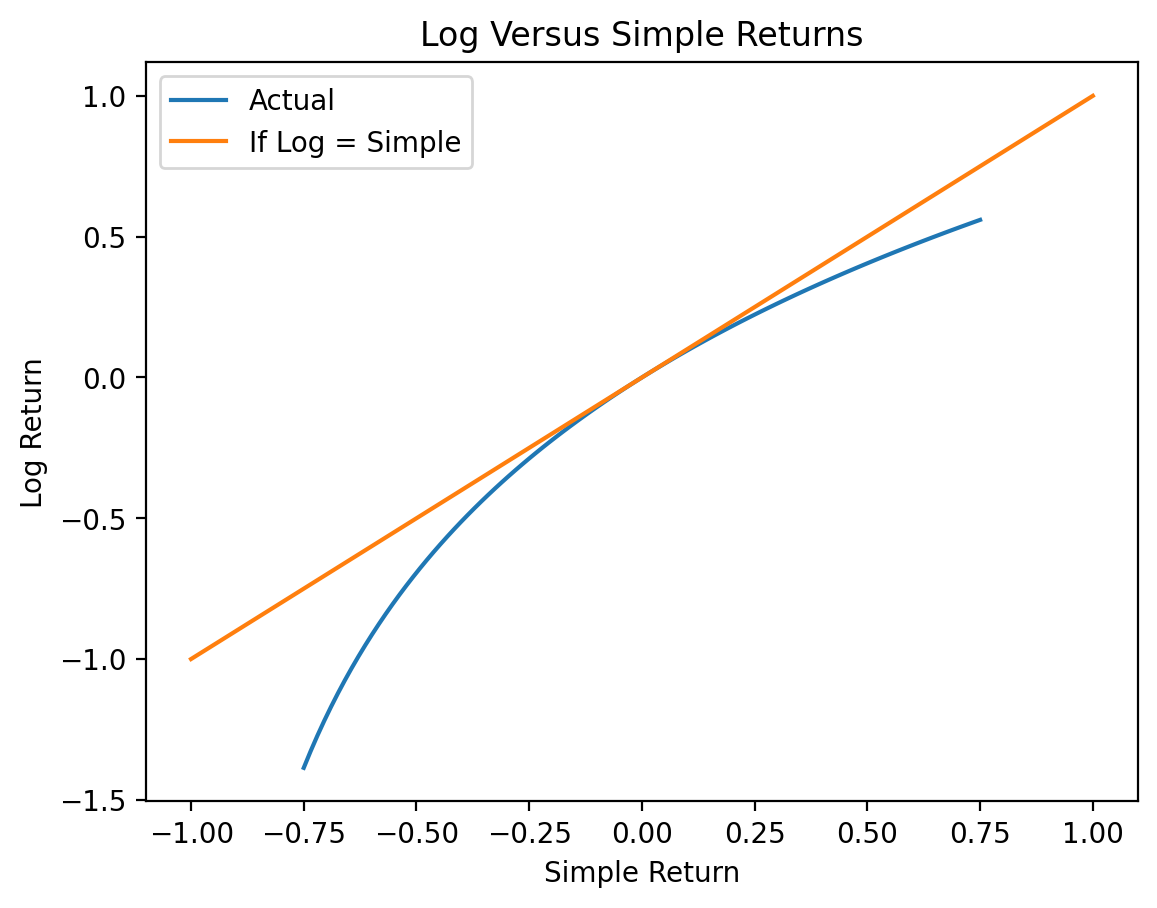
\includegraphics{herron_01_lecture_files/figure-pdf/cell-15-output-1.png}

}

\end{figure}

\hypertarget{simple-return-advantage-portfolio-calculations}{%
\subsection{Simple Return Advantage: Portfolio
Calculations}\label{simple-return-advantage-portfolio-calculations}}

We can only perform portfolio calculations with simple returns. For a
portfolio of \(N\) assets with portfolio weights \(w_i\), the portfolio
return \(R_{p}\) is the weighted average of the returns of its assets,
\(R_{p} = \sum_{i=1}^N w_i R_{i}\). For two stocks with portfolio
weights of 50\%, our portfolio return is
\(R_{portfolio} = 0.5 R_1 + 0.5 R_2 = \frac{R_1 + R_2}{2}\). However, we
cannot calculate portfolio returns with log returns because the sum of
logs is the log of products.

\textbf{\emph{We cannot calculate portfolio returns as the weighted
average of log returns.}}

\hypertarget{log-return-advantage-log-returns-are-additive}{%
\subsection{Log Return Advantage: Log Returns are
Additive}\label{log-return-advantage-log-returns-are-additive}}

The advantage of log returns is that we can compound log returns with
addition. The additive property of log returns makes code simple,
computations fast, and proofs easy when we compound returns over
multiple periods.

We compound returns from \(t=0\) to \(t=T\) as follows:
\[1 + R_{0, T} = (1 + R_1) \times (1 + R_2) \times \dots \times (1 + R_T)\]

Next, we take the log of both sides of the previous equation and use the
property that the log of products is the sum of logs:
\[\log(1 + R_{0, T}) = \log((1 + R_1) \times (1 + R_2) \times \dots \times (1 + R_T)) = \log(1 + R_1) + \log(1 + R_2) + \dots + \log(1 + R_T) = \sum_{t=1}^T \log(1 + R_t)\]

Next, we exponentiate both sides of the previous equation:
\[e^{\log(1 + R_{0, T})} = e^{\sum_{t=0}^T \log(1 + R_t)}\]

Next, we use the property that \(e^{\log(x)} = x\) to simplify the
previous equation: \[1 + R_{0,T} = e^{\sum_{t=0}^T \log(1 + R_t)}\]

Finally, we subtract 1 from both sides:
\[R_{0 ,T} = e^{\sum_{t=0}^T \log(1 + R_t)} - 1\]

So, the return \(R_{0,T}\) from \(t=0\) to \(t=T\) is the exponentiated
sum of log returns. The pandas developers assume users understand the
math above and focus on optimizing sums.

The following code generates 10,000 random log returns. The
\texttt{np.random.randn()} call generates normally distributed random
numbers. To generate equivalent simple returns, we exponentiate these
log returns, then subtract one.

\begin{Shaded}
\begin{Highlighting}[]
\NormalTok{np.random.seed(}\DecValTok{42}\NormalTok{)}
\NormalTok{df2 }\OperatorTok{=}\NormalTok{ pd.DataFrame(data}\OperatorTok{=}\NormalTok{\{}\StringTok{\textquotesingle{}R\textquotesingle{}}\NormalTok{: np.exp(np.random.randn(}\DecValTok{10000}\NormalTok{)) }\OperatorTok{{-}} \DecValTok{1}\NormalTok{\})}
\NormalTok{df2}
\end{Highlighting}
\end{Shaded}

\begin{longtable}[]{@{}ll@{}}
\toprule\noalign{}
& R \\
\midrule\noalign{}
\endhead
\bottomrule\noalign{}
\endlastfoot
0 & 0.6433 \\
1 & -0.1291 \\
2 & 0.9111 \\
3 & 3.5861 \\
4 & -0.2088 \\
... & ... \\
9995 & 2.6733 \\
9996 & -0.8644 \\
9997 & -0.5060 \\
9998 & 0.6418 \\
9999 & 0.9048 \\
\end{longtable}

\begin{Shaded}
\begin{Highlighting}[]
\NormalTok{df2.describe()}
\end{Highlighting}
\end{Shaded}

\begin{longtable}[]{@{}ll@{}}
\toprule\noalign{}
& R \\
\midrule\noalign{}
\endhead
\bottomrule\noalign{}
\endlastfoot
count & 10000.0000 \\
mean & 0.6529 \\
std & 2.1918 \\
min & -0.9802 \\
25\% & -0.4896 \\
50\% & -0.0026 \\
75\% & 0.9564 \\
max & 49.7158 \\
\end{longtable}

We can time the calculation of 12-observation rolling returns. We use
\texttt{.apply()} for the simple return version because
\texttt{.rolling()} does not have a product method. We find that
\texttt{.rolling()} is slower with \texttt{.apply()} than with
\texttt{.sum()} by a factor of 2,000. \textbf{\emph{We will learn about
\texttt{.rolling()} and \texttt{.apply()} in a few weeks, but they
provide the best example of when to use log returns.}}

\begin{Shaded}
\begin{Highlighting}[]
\OperatorTok{\%\%}\NormalTok{timeit}
\NormalTok{df2[}\StringTok{\textquotesingle{}R12\_via\_simple\textquotesingle{}}\NormalTok{] }\OperatorTok{=}\NormalTok{ (}
\NormalTok{    df2[}\StringTok{\textquotesingle{}R\textquotesingle{}}\NormalTok{]}
\NormalTok{    .add(}\DecValTok{1}\NormalTok{)}
\NormalTok{    .rolling(}\DecValTok{12}\NormalTok{)}
\NormalTok{    .}\BuiltInTok{apply}\NormalTok{(}\KeywordTok{lambda}\NormalTok{ x: x.prod())}
\NormalTok{    .sub(}\DecValTok{1}\NormalTok{)}
\NormalTok{)}
\end{Highlighting}
\end{Shaded}

\begin{verbatim}
284 ms ± 80.7 ms per loop (mean ± std. dev. of 7 runs, 1 loop each)
\end{verbatim}

\begin{Shaded}
\begin{Highlighting}[]
\OperatorTok{\%\%}\NormalTok{timeit}
\NormalTok{df2[}\StringTok{\textquotesingle{}R12\_via\_log\textquotesingle{}}\NormalTok{] }\OperatorTok{=}\NormalTok{ (}
\NormalTok{    df2[}\StringTok{\textquotesingle{}R\textquotesingle{}}\NormalTok{]}
\NormalTok{    .add(}\DecValTok{1}\NormalTok{)}
\NormalTok{    .pipe(np.log)}
\NormalTok{    .rolling(}\DecValTok{12}\NormalTok{)}
\NormalTok{    .}\BuiltInTok{sum}\NormalTok{()}
\NormalTok{    .pipe(np.exp)}
\NormalTok{    .sub(}\DecValTok{1}\NormalTok{)}
\NormalTok{)}
\end{Highlighting}
\end{Shaded}

\begin{verbatim}
557 µs ± 60.6 µs per loop (mean ± std. dev. of 7 runs, 1,000 loops each)
\end{verbatim}

\begin{Shaded}
\begin{Highlighting}[]
\NormalTok{df2.head(}\DecValTok{15}\NormalTok{)}
\end{Highlighting}
\end{Shaded}

\begin{longtable}[]{@{}llll@{}}
\toprule\noalign{}
& R & R12\_via\_simple & R12\_via\_log \\
\midrule\noalign{}
\endhead
\bottomrule\noalign{}
\endlastfoot
0 & 0.6433 & NaN & NaN \\
1 & -0.1291 & NaN & NaN \\
2 & 0.9111 & NaN & NaN \\
3 & 3.5861 & NaN & NaN \\
4 & -0.2088 & NaN & NaN \\
5 & -0.2087 & NaN & NaN \\
6 & 3.8511 & NaN & NaN \\
7 & 1.1542 & NaN & NaN \\
8 & -0.3747 & NaN & NaN \\
9 & 0.7204 & NaN & NaN \\
10 & -0.3709 & NaN & NaN \\
11 & -0.3723 & 33.8643 & 33.8643 \\
12 & 0.2737 & 26.0236 & 26.0236 \\
13 & -0.8524 & 3.5800 & 3.5800 \\
14 & -0.8218 & -0.5730 & -0.5730 \\
\end{longtable}

\begin{Shaded}
\begin{Highlighting}[]
\NormalTok{np.allclose(df2[}\StringTok{\textquotesingle{}R12\_via\_simple\textquotesingle{}}\NormalTok{], df2[}\StringTok{\textquotesingle{}R12\_via\_log\textquotesingle{}}\NormalTok{], equal\_nan}\OperatorTok{=}\VariableTok{True}\NormalTok{)}
\end{Highlighting}
\end{Shaded}

\begin{verbatim}
True
\end{verbatim}

These two approaches calculate the same return, but the simple-return
approach is 1,000 times slower than the log-return approach!

\textbf{\emph{We can use log returns to calculate total returns very
quickly!}}

\hypertarget{portfolio-math}{%
\section{Portfolio Math}\label{portfolio-math}}

Portfolio return \(R_{p}\) is the weighted average of its asset returns,
so \(R_{p} = \sum_{i=1}^N w_i R_{i}\). Here \(N\) is the number of
assets, and \(w_i\) is the weight on asset \(i\).

\hypertarget{the-1n-portfolio}{%
\subsection{The 1/N Portfolio}\label{the-1n-portfolio}}

The \(\frac{1}{N}\) portfolio equally weights portfolio assets, so
\(w_1 = w_2 = \dots = w_N = \frac{1}{N}\). We typically rebalance the
\(\frac{1}{N}\) portfolio every period. If \(w_i = \frac{1}{N}\), then
\(R_{p} = \sum_{i=1}^N \frac{1}{N} R_{i} = \frac{\sum_{i=1}^N R_i}{N} = \bar{R}\).
Therefore, we can use \texttt{.mean()} to calculate \(\frac{1}{N}\)
portfolio returns.

\begin{Shaded}
\begin{Highlighting}[]
\NormalTok{returns }\OperatorTok{=}\NormalTok{ df[}\StringTok{\textquotesingle{}Adj Close\textquotesingle{}}\NormalTok{].pct\_change().loc[}\StringTok{\textquotesingle{}2023\textquotesingle{}}\NormalTok{]}

\NormalTok{returns}
\end{Highlighting}
\end{Shaded}

\begin{longtable}[]{@{}lllllll@{}}
\toprule\noalign{}
& AAPL & AMZN & GOOG & MSFT & NVDA & TSLA \\
Date & & & & & & \\
\midrule\noalign{}
\endhead
\bottomrule\noalign{}
\endlastfoot
2023-01-03 & -0.0374 & 0.0217 & 0.0109 & -0.0010 & -0.0205 & -0.1224 \\
2023-01-04 & 0.0103 & -0.0079 & -0.0110 & -0.0437 & 0.0303 & 0.0512 \\
2023-01-05 & -0.0106 & -0.0237 & -0.0219 & -0.0296 & -0.0328 &
-0.0290 \\
2023-01-06 & 0.0368 & 0.0356 & 0.0160 & 0.0118 & 0.0416 & 0.0247 \\
2023-01-09 & 0.0041 & 0.0149 & 0.0073 & 0.0097 & 0.0518 & 0.0593 \\
... & ... & ... & ... & ... & ... & ... \\
2023-12-22 & -0.0055 & -0.0027 & 0.0065 & 0.0028 & -0.0033 & -0.0077 \\
2023-12-26 & -0.0028 & -0.0001 & 0.0007 & 0.0002 & 0.0092 & 0.0161 \\
2023-12-27 & 0.0005 & -0.0005 & -0.0097 & -0.0016 & 0.0028 & 0.0188 \\
2023-12-28 & 0.0022 & 0.0003 & -0.0011 & 0.0032 & 0.0021 & -0.0316 \\
2023-12-29 & -0.0054 & -0.0094 & -0.0025 & 0.0020 & 0.0000 & -0.0186 \\
\end{longtable}

\begin{Shaded}
\begin{Highlighting}[]
\NormalTok{returns.mean()}
\end{Highlighting}
\end{Shaded}

\begin{verbatim}
AAPL   0.0017
AMZN   0.0026
GOOG   0.0020
MSFT   0.0020
NVDA   0.0053
TSLA   0.0034
dtype: float64
\end{verbatim}

\begin{Shaded}
\begin{Highlighting}[]
\NormalTok{rp\_1 }\OperatorTok{=}\NormalTok{ returns.mean(axis}\OperatorTok{=}\DecValTok{1}\NormalTok{)}
\NormalTok{rp\_1}
\end{Highlighting}
\end{Shaded}

\begin{verbatim}
Date
2023-01-03   -0.0248
2023-01-04    0.0049
2023-01-05   -0.0246
2023-01-06    0.0278
2023-01-09    0.0245
               ...  
2023-12-22   -0.0017
2023-12-26    0.0039
2023-12-27    0.0017
2023-12-28   -0.0041
2023-12-29   -0.0056
Length: 250, dtype: float64
\end{verbatim}

\textbf{\emph{Note that when we apply the same portfolio weights every
period, we rebalance at the same frequency as the returns data.}} If we
have daily data, rebalance daily. If we have monthly data, we rebalance
monthly, and so on.

\hypertarget{a-more-general-solution}{%
\subsection{A More General Solution}\label{a-more-general-solution}}

If we combine weights into vector \(w\) and the time series of asset
returns into matrix \(\mathbf{R}\), then we can calculate the time
series of portfolio returns as \(R_p = w^T \mathbf{R}\). The pandas
version of this calculation is \texttt{R.dot(w)}, where \texttt{R} is a
data frame of asset returns and \texttt{w} is a series of portfolio
weights. We can use this approach to calculate \(\frac{1}{N}\) portfolio
returns, too.

\begin{Shaded}
\begin{Highlighting}[]
\NormalTok{weights }\OperatorTok{=}\NormalTok{ np.ones(returns.shape[}\DecValTok{1}\NormalTok{]) }\OperatorTok{/}\NormalTok{ returns.shape[}\DecValTok{1}\NormalTok{]}
\NormalTok{weights}
\end{Highlighting}
\end{Shaded}

\begin{verbatim}
array([0.1667, 0.1667, 0.1667, 0.1667, 0.1667, 0.1667])
\end{verbatim}

\begin{Shaded}
\begin{Highlighting}[]
\NormalTok{rp\_2 }\OperatorTok{=}\NormalTok{ returns.dot(weights)}
\NormalTok{rp\_2}
\end{Highlighting}
\end{Shaded}

\begin{verbatim}
Date
2023-01-03   -0.0248
2023-01-04    0.0049
2023-01-05   -0.0246
2023-01-06    0.0278
2023-01-09    0.0245
               ...  
2023-12-22   -0.0017
2023-12-26    0.0039
2023-12-27    0.0017
2023-12-28   -0.0041
2023-12-29   -0.0056
Length: 250, dtype: float64
\end{verbatim}

Both approaches give the same answer!

\begin{Shaded}
\begin{Highlighting}[]
\NormalTok{np.allclose(rp\_1, rp\_2, equal\_nan}\OperatorTok{=}\VariableTok{True}\NormalTok{)}
\end{Highlighting}
\end{Shaded}

\begin{verbatim}
True
\end{verbatim}

\hypertarget{herron-topic-1---practice-for-section-02}{%
\chapter{Herron Topic 1 - Practice for Section
02}\label{herron-topic-1---practice-for-section-02}}

\hypertarget{announcements-16}{%
\section{Announcements}\label{announcements-16}}

\begin{enumerate}
\def\labelenumi{\arabic{enumi}.}
\tightlist
\item
  DataCamp

  \begin{enumerate}
  \def\labelenumii{\arabic{enumii}.}
  \tightlist
  \item
    \emph{Data Manipulation with pandas} due by Friday, 2/9, at 11:59 PM
  \item
    \emph{Joining Data with pandas} due by Friday, 2/16, at 11:59 PM
  \item
    \emph{Earn 10,000 XP} due by Friday, 3/15, at 11:59 PM
  \end{enumerate}
\item
  I posted Project 1 to Canvas

  \begin{enumerate}
  \def\labelenumii{\arabic{enumii}.}
  \tightlist
  \item
    Slides and notebook due by Friday, 2/23, at 11:59 PM
  \item
    Keep joining teams and let me know if you need help
  \end{enumerate}
\end{enumerate}

\hypertarget{minute-recap-15}{%
\section{10-Minute Recap}\label{minute-recap-15}}

\begin{Shaded}
\begin{Highlighting}[]
\ImportTok{import}\NormalTok{ matplotlib.pyplot }\ImportTok{as}\NormalTok{ plt}
\ImportTok{import}\NormalTok{ numpy }\ImportTok{as}\NormalTok{ np}
\ImportTok{import}\NormalTok{ pandas }\ImportTok{as}\NormalTok{ pd}
\ImportTok{import}\NormalTok{ pandas\_datareader }\ImportTok{as}\NormalTok{ pdr}
\ImportTok{import}\NormalTok{ yfinance }\ImportTok{as}\NormalTok{ yf}
\end{Highlighting}
\end{Shaded}

\begin{Shaded}
\begin{Highlighting}[]
\OperatorTok{\%}\NormalTok{precision }\DecValTok{4}
\NormalTok{pd.options.display.float\_format }\OperatorTok{=} \StringTok{\textquotesingle{}}\SpecialCharTok{\{:.4f\}}\StringTok{\textquotesingle{}}\NormalTok{.}\BuiltInTok{format}
\OperatorTok{\%}\NormalTok{config InlineBackend.figure\_format }\OperatorTok{=} \StringTok{\textquotesingle{}retina\textquotesingle{}}
\end{Highlighting}
\end{Shaded}

First, we will use two packages to download data from the web:

\begin{enumerate}
\def\labelenumi{\arabic{enumi}.}
\tightlist
\item
  \texttt{yfinance} for Yahoo! Finance data
\item
  \texttt{pandas-datareader} for Ken French data (and FRED data)
\end{enumerate}

Second, there are ``simple returns'' and ``log returns''

\begin{enumerate}
\def\labelenumi{\arabic{enumi}.}
\tightlist
\item
  Simple returns are the returns that investors receive that we learned
  in FINA 6331 and FINA 6333:
  \(r_t = \frac{p_t + d_t - p_{t-1}}{p_{t-1}}\)
\item
  Log returns are the log of one plus simple returns. Why do we use
  them?

  \begin{enumerate}
  \def\labelenumii{\arabic{enumii}.}
  \tightlist
  \item
    \textbf{\emph{Log returns are additive}}, while simple returns are
    multiplicative. This additive property makes math really easy with
    log returns:
    \(\log(\prod_{t=0}^T (1 + r_t)) = \sum_{t=0}^T \log(1+r_t)\), so
    \(r_{0,T} = \prod_{t=0}^T (1 + r_t) - 1 = e^{\sum_{t=0}^T \log(1+r_t)} - 1\)
  \item
    \textbf{\emph{Log returns are almost normally distributed}}
  \end{enumerate}
\end{enumerate}

\textbf{\emph{We will almost always use simple returns.}} The exeception
is time-consuming calculations, which we will often do in log returns to
save us time.

Third, we can calculate portfolio returns a few ways

\begin{enumerate}
\def\labelenumi{\arabic{enumi}.}
\tightlist
\item
  We can calculate equally-weighted returns with
  \texttt{returns.mean(axis=1)}, \textbf{\emph{rebalanced at the same
  frequency as returns}}
\item
  We can calculate any-weighted with \texttt{returns.dot(weights)},
  where \texttt{weights} is an array of portfolio weights that are not
  necessarily equally-weighted, still \textbf{\emph{rebalanced at the
  same frequency as returns}}
\end{enumerate}

\hypertarget{practice-16}{%
\section{Practice}\label{practice-16}}

\hypertarget{download-all-available-daily-price-data-for-tickers-tsla-f-aapl-amzn-and-meta-to-data-frame-prices}{%
\subsection{\texorpdfstring{Download all available daily price data for
tickers TSLA, F, AAPL, AMZN, and META to data frame
\texttt{prices}}{Download all available daily price data for tickers TSLA, F, AAPL, AMZN, and META to data frame prices}}\label{download-all-available-daily-price-data-for-tickers-tsla-f-aapl-amzn-and-meta-to-data-frame-prices}}

\begin{Shaded}
\begin{Highlighting}[]
\NormalTok{tickers }\OperatorTok{=} \StringTok{\textquotesingle{}TSLA F AAPL AMZN META\textquotesingle{}}
\CommentTok{\# tickers = [\textquotesingle{}TSLA\textquotesingle{}, \textquotesingle{}F\textquotesingle{},  \textquotesingle{}AAPL\textquotesingle{}, \textquotesingle{}AMZN\textquotesingle{}, \textquotesingle{}META\textquotesingle{}]}
\NormalTok{prices }\OperatorTok{=}\NormalTok{ yf.download(tickers}\OperatorTok{=}\NormalTok{tickers)}

\NormalTok{prices}
\end{Highlighting}
\end{Shaded}

\begin{verbatim}
[*********************100%%**********************]  5 of 5 completed
\end{verbatim}

\begin{longtable}[]{@{}llllllllllllllllllllll@{}}
\toprule\noalign{}
&
\multicolumn{5}{>{\raggedright\arraybackslash}p{(\columnwidth - 42\tabcolsep) * \real{0.0000} + 8\tabcolsep}}{%
Adj Close} &
\multicolumn{5}{>{\raggedright\arraybackslash}p{(\columnwidth - 42\tabcolsep) * \real{0.0000} + 8\tabcolsep}}{%
Close} & ... &
\multicolumn{5}{>{\raggedright\arraybackslash}p{(\columnwidth - 42\tabcolsep) * \real{0.0000} + 8\tabcolsep}}{%
Open} &
\multicolumn{5}{>{\raggedright\arraybackslash}p{(\columnwidth - 42\tabcolsep) * \real{0.0000} + 8\tabcolsep}@{}}{%
Volume} \\
& AAPL & AMZN & F & META & TSLA & AAPL & AMZN & F & META & TSLA & ... &
AAPL & AMZN & F & META & TSLA & AAPL & AMZN & F & META & TSLA \\
Date & & & & & & & & & & & & & & & & & & & & & \\
\midrule\noalign{}
\endhead
\bottomrule\noalign{}
\endlastfoot
1972-06-01 & NaN & NaN & 0.2419 & NaN & NaN & NaN & NaN & 2.1532 & NaN &
NaN & ... & NaN & NaN & 0.0000 & NaN & NaN & NaN & NaN & 1091238 & NaN &
NaN \\
1972-06-02 & NaN & NaN & 0.2414 & NaN & NaN & NaN & NaN & 2.1492 & NaN &
NaN & ... & NaN & NaN & 2.1532 & NaN & NaN & NaN & NaN & 1174468 & NaN &
NaN \\
1972-06-05 & NaN & NaN & 0.2414 & NaN & NaN & NaN & NaN & 2.1492 & NaN &
NaN & ... & NaN & NaN & 2.1492 & NaN & NaN & NaN & NaN & 5209582 & NaN &
NaN \\
1972-06-06 & NaN & NaN & 0.2387 & NaN & NaN & NaN & NaN & 2.1248 & NaN &
NaN & ... & NaN & NaN & 2.1492 & NaN & NaN & NaN & NaN & 1424158 & NaN &
NaN \\
1972-06-07 & NaN & NaN & 0.2373 & NaN & NaN & NaN & NaN & 2.1127 & NaN &
NaN & ... & NaN & NaN & 2.1248 & NaN & NaN & NaN & NaN & 675088 & NaN &
NaN \\
... & ... & ... & ... & ... & ... & ... & ... & ... & ... & ... & ... &
... & ... & ... & ... & ... & ... & ... & ... & ... & ... \\
2024-02-05 & 187.6800 & 170.3100 & 11.5900 & 459.4100 & 181.0600 &
187.6800 & 170.3100 & 11.5900 & 459.4100 & 181.0600 & ... & 188.1500 &
170.2000 & 12.0100 & 469.8800 & 184.2600 & 69668800.0000 & 55081300.0000
& 81026800 & 40832400.0000 & 134294400.0000 \\
2024-02-06 & 189.3000 & 169.1500 & 12.0700 & 454.7200 & 185.1000 &
189.3000 & 169.1500 & 12.0700 & 454.7200 & 185.1000 & ... & 186.8600 &
169.3900 & 11.6400 & 464.0000 & 177.2100 & 43490800.0000 & 42505500.0000
& 98636800 & 21655200.0000 & 122676000.0000 \\
2024-02-07 & 189.4100 & 170.5300 & 12.8000 & 469.5900 & 187.5800 &
189.4100 & 170.5300 & 12.8000 & 469.5900 & 187.5800 & ... & 190.6400 &
169.4800 & 12.7300 & 458.0000 & 188.1800 & 53439000.0000 & 47174100.0000
& 137224000 & 23066000.0000 & 111535200.0000 \\
2024-02-08 & 188.3200 & 169.8400 & 12.8300 & 470.0000 & 189.5600 &
188.3200 & 169.8400 & 12.8300 & 470.0000 & 189.5600 & ... & 189.3900 &
169.6500 & 12.8700 & 468.3200 & 189.0000 & 40962000.0000 & 42316500.0000
& 68653900 & 18815100.0000 & 83034000.0000 \\
2024-02-09 & 188.8500 & 174.4500 & 12.6800 & 468.1100 & 193.5700 &
188.8500 & 174.4500 & 12.6800 & 468.1100 & 193.5700 & ... & 188.6500 &
170.9000 & 12.8100 & 472.9500 & 190.1800 & 43728065.0000 & 56886544.0000
& 46925766 & 18159624.0000 & 84009121.0000 \\
\end{longtable}

\hypertarget{calculate-all-available-daily-returns-and-save-to-data-frame-returns}{%
\subsection{\texorpdfstring{Calculate all available daily returns and
save to data frame
\texttt{returns}}{Calculate all available daily returns and save to data frame returns}}\label{calculate-all-available-daily-returns-and-save-to-data-frame-returns}}

\begin{Shaded}
\begin{Highlighting}[]
\NormalTok{returns }\OperatorTok{=}\NormalTok{ (}
\NormalTok{    prices[}\StringTok{\textquotesingle{}Adj Close\textquotesingle{}}\NormalTok{] }\CommentTok{\# slice adj close}
\NormalTok{    .iloc[:}\OperatorTok{{-}}\DecValTok{1}\NormalTok{] }\CommentTok{\# drop the last price because it might be intraday (i.e., not a close)}
\NormalTok{    .pct\_change() }\CommentTok{\# calculate simple returns}
\NormalTok{)}

\NormalTok{returns}
\end{Highlighting}
\end{Shaded}

\begin{longtable}[]{@{}llllll@{}}
\toprule\noalign{}
& AAPL & AMZN & F & META & TSLA \\
Date & & & & & \\
\midrule\noalign{}
\endhead
\bottomrule\noalign{}
\endlastfoot
1972-06-01 & NaN & NaN & NaN & NaN & NaN \\
1972-06-02 & NaN & NaN & -0.0019 & NaN & NaN \\
1972-06-05 & NaN & NaN & 0.0000 & NaN & NaN \\
1972-06-06 & NaN & NaN & -0.0113 & NaN & NaN \\
1972-06-07 & NaN & NaN & -0.0057 & NaN & NaN \\
... & ... & ... & ... & ... & ... \\
2024-02-02 & -0.0054 & 0.0787 & 0.0033 & 0.2032 & -0.0050 \\
2024-02-05 & 0.0098 & -0.0087 & -0.0453 & -0.0328 & -0.0365 \\
2024-02-06 & 0.0086 & -0.0068 & 0.0414 & -0.0102 & 0.0223 \\
2024-02-07 & 0.0006 & 0.0082 & 0.0605 & 0.0327 & 0.0134 \\
2024-02-08 & -0.0058 & -0.0040 & 0.0023 & 0.0009 & 0.0106 \\
\end{longtable}

\hypertarget{slices-returns-for-the-2020s-and-assign-to-returns_2020s}{%
\subsection{\texorpdfstring{Slices returns for the 2020s and assign to
\texttt{returns\_2020s}}{Slices returns for the 2020s and assign to returns\_2020s}}\label{slices-returns-for-the-2020s-and-assign-to-returns_2020s}}

\begin{Shaded}
\begin{Highlighting}[]
\NormalTok{returns\_2020s }\OperatorTok{=}\NormalTok{ returns.loc[}\StringTok{\textquotesingle{}2020\textquotesingle{}}\NormalTok{:] }\CommentTok{\# always use an unambiguos date format, like YYYY{-}MM{-}DD}

\NormalTok{returns\_2020s}
\end{Highlighting}
\end{Shaded}

\begin{longtable}[]{@{}llllll@{}}
\toprule\noalign{}
& AAPL & AMZN & F & META & TSLA \\
Date & & & & & \\
\midrule\noalign{}
\endhead
\bottomrule\noalign{}
\endlastfoot
2020-01-02 & 0.0228 & 0.0272 & 0.0129 & 0.0221 & 0.0285 \\
2020-01-03 & -0.0097 & -0.0121 & -0.0223 & -0.0053 & 0.0296 \\
2020-01-06 & 0.0080 & 0.0149 & -0.0054 & 0.0188 & 0.0193 \\
2020-01-07 & -0.0047 & 0.0021 & 0.0098 & 0.0022 & 0.0388 \\
2020-01-08 & 0.0161 & -0.0078 & 0.0000 & 0.0101 & 0.0492 \\
... & ... & ... & ... & ... & ... \\
2024-02-02 & -0.0054 & 0.0787 & 0.0033 & 0.2032 & -0.0050 \\
2024-02-05 & 0.0098 & -0.0087 & -0.0453 & -0.0328 & -0.0365 \\
2024-02-06 & 0.0086 & -0.0068 & 0.0414 & -0.0102 & 0.0223 \\
2024-02-07 & 0.0006 & 0.0082 & 0.0605 & 0.0327 & 0.0134 \\
2024-02-08 & -0.0058 & -0.0040 & 0.0023 & 0.0009 & 0.0106 \\
\end{longtable}

\begin{center}\rule{0.5\linewidth}{0.5pt}\end{center}

What if we want a more complicated slice? We can combine
\texttt{.loc{[}{]}} and Boolean conditions!

\begin{Shaded}
\begin{Highlighting}[]
\NormalTok{returns.loc[}
\NormalTok{    (returns.index.year }\OperatorTok{==} \DecValTok{2020}\NormalTok{) }\OperatorTok{\&}
\NormalTok{    ((returns.index.month }\OperatorTok{==} \DecValTok{1}\NormalTok{) }\OperatorTok{|}\NormalTok{ (returns.index.month }\OperatorTok{==} \DecValTok{12}\NormalTok{))}
\NormalTok{]}
\end{Highlighting}
\end{Shaded}

\begin{longtable}[]{@{}llllll@{}}
\toprule\noalign{}
& AAPL & AMZN & F & META & TSLA \\
Date & & & & & \\
\midrule\noalign{}
\endhead
\bottomrule\noalign{}
\endlastfoot
2020-01-02 & 0.0228 & 0.0272 & 0.0129 & 0.0221 & 0.0285 \\
2020-01-03 & -0.0097 & -0.0121 & -0.0223 & -0.0053 & 0.0296 \\
2020-01-06 & 0.0080 & 0.0149 & -0.0054 & 0.0188 & 0.0193 \\
2020-01-07 & -0.0047 & 0.0021 & 0.0098 & 0.0022 & 0.0388 \\
2020-01-08 & 0.0161 & -0.0078 & 0.0000 & 0.0101 & 0.0492 \\
2020-01-09 & 0.0212 & 0.0048 & 0.0011 & 0.0143 & -0.0219 \\
2020-01-10 & 0.0023 & -0.0094 & -0.0011 & -0.0011 & -0.0066 \\
2020-01-13 & 0.0214 & 0.0043 & -0.0011 & 0.0177 & 0.0977 \\
2020-01-14 & -0.0135 & -0.0116 & 0.0054 & -0.0128 & 0.0249 \\
2020-01-15 & -0.0043 & -0.0040 & -0.0108 & 0.0095 & -0.0361 \\
2020-01-16 & 0.0125 & 0.0085 & -0.0022 & 0.0028 & -0.0097 \\
2020-01-17 & 0.0111 & -0.0070 & -0.0011 & 0.0017 & -0.0058 \\
2020-01-21 & -0.0068 & 0.0146 & 0.0055 & -0.0032 & 0.0719 \\
2020-01-22 & 0.0036 & -0.0024 & -0.0054 & -0.0005 & 0.0409 \\
2020-01-23 & 0.0048 & -0.0015 & -0.0022 & -0.0070 & 0.0046 \\
2020-01-24 & -0.0029 & -0.0122 & -0.0153 & -0.0083 & -0.0129 \\
2020-01-27 & -0.0294 & -0.0179 & -0.0122 & -0.0141 & -0.0120 \\
2020-01-28 & 0.0283 & 0.0136 & 0.0090 & 0.0136 & 0.0159 \\
2020-01-29 & 0.0209 & 0.0026 & 0.0045 & 0.0250 & 0.0249 \\
2020-01-30 & -0.0014 & 0.0068 & -0.0023 & -0.0614 & 0.1030 \\
2020-01-31 & -0.0443 & 0.0738 & -0.0023 & -0.0364 & 0.0152 \\
2020-12-01 & 0.0308 & 0.0164 & 0.0176 & 0.0346 & 0.0302 \\
2020-12-02 & 0.0029 & -0.0051 & -0.0043 & 0.0034 & -0.0273 \\
2020-12-03 & -0.0011 & -0.0052 & 0.0011 & -0.0197 & 0.0432 \\
2020-12-04 & -0.0056 & -0.0076 & 0.0141 & -0.0076 & 0.0095 \\
2020-12-07 & 0.0123 & -0.0014 & -0.0128 & 0.0210 & 0.0713 \\
2020-12-08 & 0.0051 & 0.0061 & 0.0033 & -0.0076 & 0.0127 \\
2020-12-09 & -0.0209 & -0.0230 & 0.0216 & -0.0193 & -0.0699 \\
2020-12-10 & 0.0120 & -0.0009 & -0.0349 & -0.0029 & 0.0374 \\
2020-12-11 & -0.0067 & 0.0048 & -0.0110 & -0.0129 & -0.0272 \\
2020-12-14 & -0.0051 & 0.0130 & -0.0122 & 0.0023 & 0.0489 \\
2020-12-15 & 0.0501 & 0.0026 & 0.0269 & 0.0050 & -0.0103 \\
2020-12-16 & -0.0005 & 0.0240 & -0.0120 & 0.0004 & -0.0165 \\
2020-12-17 & 0.0070 & -0.0015 & 0.0044 & -0.0043 & 0.0532 \\
2020-12-18 & -0.0159 & -0.0106 & -0.0143 & 0.0070 & 0.0596 \\
2020-12-21 & 0.0124 & 0.0014 & -0.0022 & -0.0131 & -0.0649 \\
2020-12-22 & 0.0285 & 0.0001 & -0.0157 & -0.0209 & -0.0146 \\
2020-12-23 & -0.0070 & -0.0066 & 0.0228 & 0.0038 & 0.0088 \\
2020-12-24 & 0.0077 & -0.0039 & -0.0145 & -0.0026 & 0.0244 \\
2020-12-28 & 0.0358 & 0.0351 & 0.0034 & 0.0359 & 0.0029 \\
2020-12-29 & -0.0133 & 0.0116 & -0.0079 & -0.0008 & 0.0035 \\
2020-12-30 & -0.0085 & -0.0109 & 0.0045 & -0.0177 & 0.0432 \\
2020-12-31 & -0.0077 & -0.0088 & -0.0079 & 0.0047 & 0.0157 \\
\end{longtable}

\begin{center}\rule{0.5\linewidth}{0.5pt}\end{center}

\hypertarget{download-all-available-data-for-the-fama-and-french-daily-benchmark-factors-to-dictionary-ff_all}{%
\subsection{\texorpdfstring{Download all available data for the Fama and
French daily benchmark factors to dictionary
\texttt{ff\_all}}{Download all available data for the Fama and French daily benchmark factors to dictionary ff\_all}}\label{download-all-available-data-for-the-fama-and-french-daily-benchmark-factors-to-dictionary-ff_all}}

I often use the following code snippet to find the exact name for the
the daily benchmark factors file.

\begin{Shaded}
\begin{Highlighting}[]
\NormalTok{pdr.famafrench.get\_available\_datasets()[:}\DecValTok{5}\NormalTok{]}
\end{Highlighting}
\end{Shaded}

\begin{verbatim}
['F-F_Research_Data_Factors',
 'F-F_Research_Data_Factors_weekly',
 'F-F_Research_Data_Factors_daily',
 'F-F_Research_Data_5_Factors_2x3',
 'F-F_Research_Data_5_Factors_2x3_daily']
\end{verbatim}

\begin{Shaded}
\begin{Highlighting}[]
\NormalTok{ff\_all }\OperatorTok{=}\NormalTok{ pdr.DataReader(}
\NormalTok{    name}\OperatorTok{=}\StringTok{\textquotesingle{}F{-}F\_Research\_Data\_Factors\_daily\textquotesingle{}}\NormalTok{,}
\NormalTok{    data\_source}\OperatorTok{=}\StringTok{\textquotesingle{}famafrench\textquotesingle{}}\NormalTok{,}
\NormalTok{    start}\OperatorTok{=}\StringTok{\textquotesingle{}1900\textquotesingle{}}
\NormalTok{)}
\end{Highlighting}
\end{Shaded}

\begin{verbatim}
C:\Users\r.herron\AppData\Local\Temp\ipykernel_28696\2526882917.py:1: FutureWarning: The argument 'date_parser' is deprecated and will be removed in a future version. Please use 'date_format' instead, or read your data in as 'object' dtype and then call 'to_datetime'.
  ff_all = pdr.DataReader(
\end{verbatim}

The \texttt{DESCR} key in the dictionary tells us about the data frames
that \texttt{pandas-datareader} returns.

\begin{Shaded}
\begin{Highlighting}[]
\BuiltInTok{print}\NormalTok{(ff\_all[}\StringTok{\textquotesingle{}DESCR\textquotesingle{}}\NormalTok{])}
\end{Highlighting}
\end{Shaded}

\begin{verbatim}
F-F Research Data Factors daily
-------------------------------

This file was created by CMPT_ME_BEME_RETS_DAILY using the 202312 CRSP database. The Tbill return is the simple daily rate that, over the number of trading days in the month, compounds to 1-month TBill rate from Ibbotson and Associates Inc. Copyright 2023 Kenneth R. French

  0 : (25649 rows x 4 cols)
\end{verbatim}

\hypertarget{slice-the-daily-benchmark-factors-convert-them-to-decimal-returns-and-assign-to-ff}{%
\subsection{\texorpdfstring{Slice the daily benchmark factors, convert
them to decimal returns, and assign to
\texttt{ff}}{Slice the daily benchmark factors, convert them to decimal returns, and assign to ff}}\label{slice-the-daily-benchmark-factors-convert-them-to-decimal-returns-and-assign-to-ff}}

\begin{Shaded}
\begin{Highlighting}[]
\NormalTok{ff }\OperatorTok{=}\NormalTok{ ff\_all[}\DecValTok{0}\NormalTok{].div(}\DecValTok{100}\NormalTok{)}

\NormalTok{ff}
\end{Highlighting}
\end{Shaded}

\begin{longtable}[]{@{}lllll@{}}
\toprule\noalign{}
& Mkt-RF & SMB & HML & RF \\
Date & & & & \\
\midrule\noalign{}
\endhead
\bottomrule\noalign{}
\endlastfoot
1926-07-01 & 0.0010 & -0.0025 & -0.0027 & 0.0001 \\
1926-07-02 & 0.0045 & -0.0033 & -0.0006 & 0.0001 \\
1926-07-06 & 0.0017 & 0.0030 & -0.0039 & 0.0001 \\
1926-07-07 & 0.0009 & -0.0058 & 0.0002 & 0.0001 \\
1926-07-08 & 0.0021 & -0.0038 & 0.0019 & 0.0001 \\
... & ... & ... & ... & ... \\
2023-12-22 & 0.0021 & 0.0064 & 0.0009 & 0.0002 \\
2023-12-26 & 0.0048 & 0.0069 & 0.0046 & 0.0002 \\
2023-12-27 & 0.0016 & 0.0014 & 0.0012 & 0.0002 \\
2023-12-28 & -0.0001 & -0.0036 & 0.0003 & 0.0002 \\
2023-12-29 & -0.0043 & -0.0112 & -0.0037 & 0.0002 \\
\end{longtable}

\hypertarget{use-the-.cumprod-method-to-plot-cumulative-returns-for-these-stocks-in-the-2020s}{%
\subsection{\texorpdfstring{Use the \texttt{.cumprod()} method to plot
cumulative returns for these stocks in the
2020s}{Use the .cumprod() method to plot cumulative returns for these stocks in the 2020s}}\label{use-the-.cumprod-method-to-plot-cumulative-returns-for-these-stocks-in-the-2020s}}

We use the \texttt{.prod()} method to calculate \emph{total} returns,
because
\(r_{total} = r_{0,T} = \left[ \prod_{t=0}^T (1 + r_t) \right] -1\).

\begin{Shaded}
\begin{Highlighting}[]
\NormalTok{totret }\OperatorTok{=}\NormalTok{ (}
\NormalTok{    returns\_2020s }\CommentTok{\# returns during the 2020s}
\NormalTok{    .add(}\DecValTok{1}\NormalTok{) }\CommentTok{\# add 1 before we compound}
\NormalTok{    .prod() }\CommentTok{\# compound all returns}
\NormalTok{    .sub(}\DecValTok{1}\NormalTok{) }\CommentTok{\# subtract 1 to recover total returns}
\NormalTok{)}

\NormalTok{totret}
\end{Highlighting}
\end{Shaded}

\begin{verbatim}
AAPL   1.6331
AMZN   0.8383
F      0.6090
META   1.2899
TSLA   5.7970
dtype: float64
\end{verbatim}

\begin{Shaded}
\begin{Highlighting}[]
\NormalTok{cumret\_cumprod }\OperatorTok{=}\NormalTok{ returns\_2020s.add(}\DecValTok{1}\NormalTok{).cumprod().sub(}\DecValTok{1}\NormalTok{)}
\end{Highlighting}
\end{Shaded}

The last row in the cumulative returns data frame
\texttt{cumret\_cumprod} is the same as the total returns series
\texttt{totret}!

\begin{Shaded}
\begin{Highlighting}[]
\NormalTok{np.allclose(totret, cumret\_cumprod.iloc[}\OperatorTok{{-}}\DecValTok{1}\NormalTok{])}
\end{Highlighting}
\end{Shaded}

\begin{verbatim}
True
\end{verbatim}

We can use the \texttt{.plot()} method to plot these cumulative returns!

\begin{Shaded}
\begin{Highlighting}[]
\NormalTok{cumret\_cumprod.mul(}\DecValTok{100}\NormalTok{).plot()}

\CommentTok{\# https://stackoverflow.com/questions/25973581/how{-}to{-}format{-}axis{-}number{-}format{-}to{-}thousands{-}with{-}a{-}comma}
\ImportTok{from}\NormalTok{ matplotlib }\ImportTok{import}\NormalTok{ ticker}
\NormalTok{plt.gca().get\_yaxis().set\_major\_formatter(ticker.FuncFormatter(}\KeywordTok{lambda}\NormalTok{ x, p: }\BuiltInTok{format}\NormalTok{(}\BuiltInTok{int}\NormalTok{(x), }\StringTok{\textquotesingle{},\textquotesingle{}}\NormalTok{)))}

\NormalTok{plt.ylabel(}\StringTok{\textquotesingle{}Cumulative Return (\%)\textquotesingle{}}\NormalTok{)}
\NormalTok{plt.title(}\SpecialStringTok{f\textquotesingle{}Cumulative Returns}\CharTok{\textbackslash{}n}\SpecialStringTok{ from }\SpecialCharTok{\{}\NormalTok{cumret\_cumprod}\SpecialCharTok{.}\NormalTok{index}\SpecialCharTok{.}\BuiltInTok{min}\NormalTok{()}\SpecialCharTok{:}\OperatorTok{\%}\NormalTok{b }\OperatorTok{\%}\NormalTok{Y}\SpecialCharTok{\}}\SpecialStringTok{ to }\SpecialCharTok{\{}\NormalTok{cumret\_cumprod}\SpecialCharTok{.}\NormalTok{index}\SpecialCharTok{.}\BuiltInTok{max}\NormalTok{()}\SpecialCharTok{:}\OperatorTok{\%}\NormalTok{b }\OperatorTok{\%}\NormalTok{Y}\SpecialCharTok{\}}\SpecialStringTok{\textquotesingle{}}\NormalTok{)}
\NormalTok{plt.show()}
\end{Highlighting}
\end{Shaded}

\begin{figure}[H]

{\centering 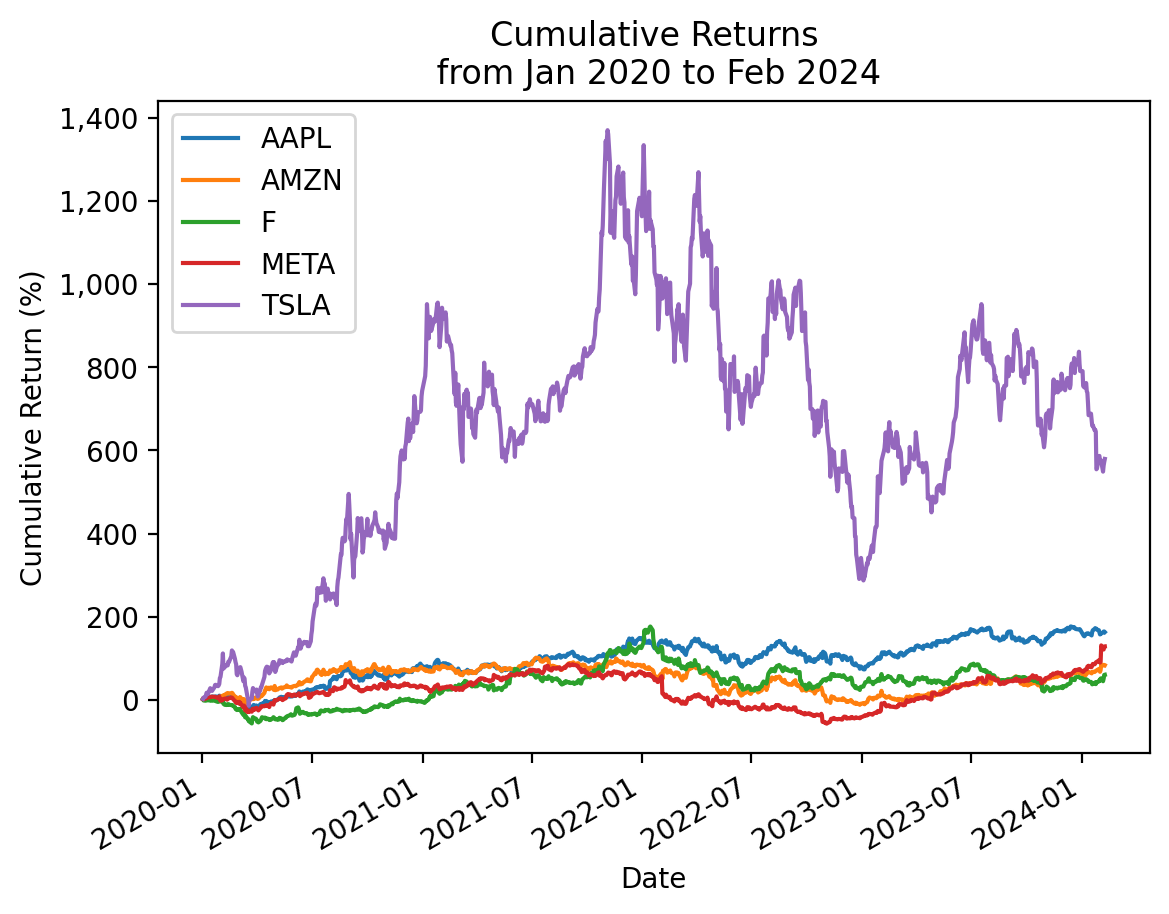
\includegraphics{herron_01_practice_02_files/figure-pdf/cell-15-output-1.png}

}

\end{figure}

We can also \texttt{plt.plot()}, but lose a few of the formatting
defaults built into the pandas method \texttt{.plot()}.

\begin{Shaded}
\begin{Highlighting}[]
\NormalTok{plt.plot(cumret\_cumprod.mul(}\DecValTok{100}\NormalTok{))}
\end{Highlighting}
\end{Shaded}

\begin{figure}[H]

{\centering 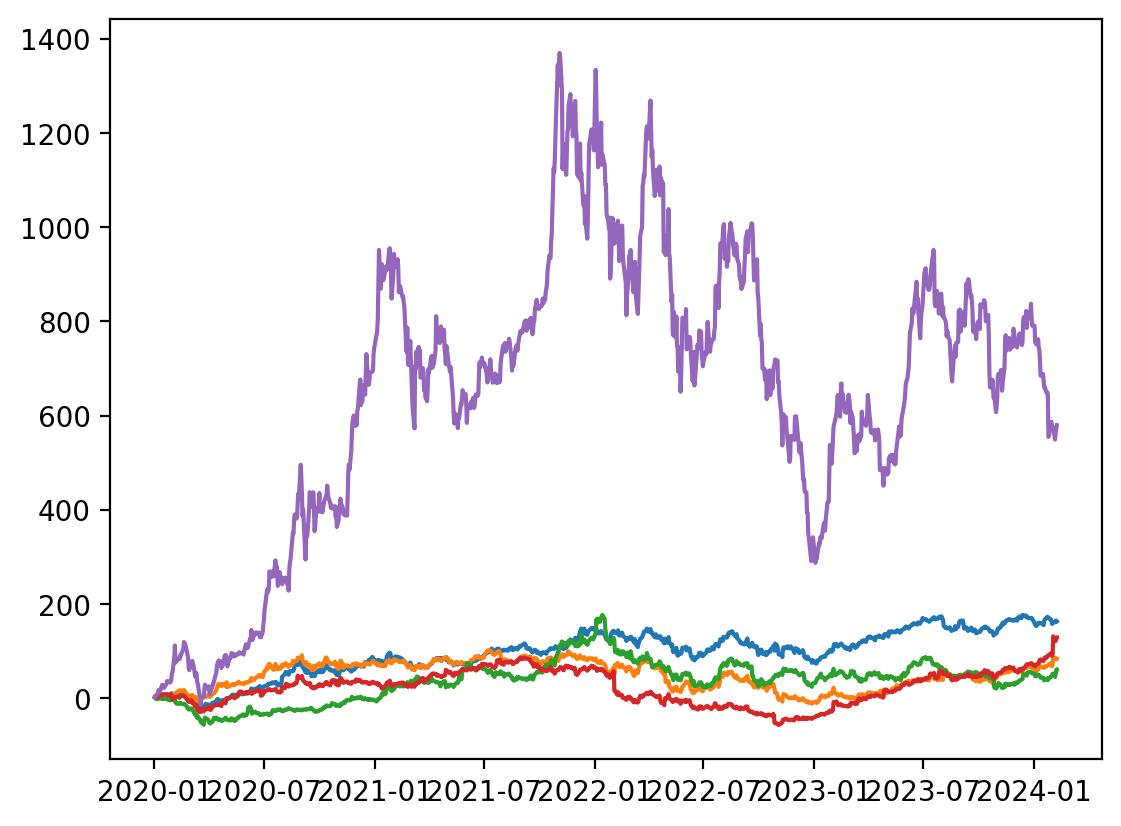
\includegraphics{herron_01_practice_02_files/figure-pdf/cell-16-output-1.png}

}

\end{figure}

\hypertarget{use-the-.cumsum-method-with-log-returns-to-plot-cumulative-returns-for-these-stocks-in-the-2020s}{%
\subsection{\texorpdfstring{Use the \texttt{.cumsum()} method with log
returns to plot cumulative returns for these stocks in the
2020s}{Use the .cumsum() method with log returns to plot cumulative returns for these stocks in the 2020s}}\label{use-the-.cumsum-method-with-log-returns-to-plot-cumulative-returns-for-these-stocks-in-the-2020s}}

\begin{Shaded}
\begin{Highlighting}[]
\NormalTok{cumret\_cumsum }\OperatorTok{=}\NormalTok{ (}
\NormalTok{    returns\_2020s}
\NormalTok{    .pipe(np.log1p) }\CommentTok{\# converts simple returns to log returns}
\NormalTok{    .cumsum() }\CommentTok{\# log returns are additive}
\NormalTok{    .pipe(np.expm1) }\CommentTok{\# converts log returns to simple returns}
\NormalTok{)}
\CommentTok{\# cumret\_cumsum = returns\_2020s.add(1).pipe(np.log).cumsum().pipe(np.exp).sub(1)}
\end{Highlighting}
\end{Shaded}

\begin{Shaded}
\begin{Highlighting}[]
\NormalTok{np.allclose(totret, cumret\_cumsum.iloc[}\OperatorTok{{-}}\DecValTok{1}\NormalTok{])}
\end{Highlighting}
\end{Shaded}

\begin{verbatim}
True
\end{verbatim}

\begin{Shaded}
\begin{Highlighting}[]
\NormalTok{cumret\_cumsum.mul(}\DecValTok{100}\NormalTok{).plot()}

\CommentTok{\# https://stackoverflow.com/questions/25973581/how{-}to{-}format{-}axis{-}number{-}format{-}to{-}thousands{-}with{-}a{-}comma}
\ImportTok{from}\NormalTok{ matplotlib }\ImportTok{import}\NormalTok{ ticker}
\NormalTok{plt.gca().get\_yaxis().set\_major\_formatter(ticker.FuncFormatter(}\KeywordTok{lambda}\NormalTok{ x, p: }\BuiltInTok{format}\NormalTok{(}\BuiltInTok{int}\NormalTok{(x), }\StringTok{\textquotesingle{},\textquotesingle{}}\NormalTok{)))}

\NormalTok{plt.ylabel(}\StringTok{\textquotesingle{}Cumulative Return (\%)\textquotesingle{}}\NormalTok{)}
\NormalTok{plt.title(}\SpecialStringTok{f\textquotesingle{}Cumulative Returns}\CharTok{\textbackslash{}n}\SpecialStringTok{ from }\SpecialCharTok{\{}\NormalTok{cumret\_cumsum}\SpecialCharTok{.}\NormalTok{index}\SpecialCharTok{.}\BuiltInTok{min}\NormalTok{()}\SpecialCharTok{:}\OperatorTok{\%}\NormalTok{b }\OperatorTok{\%}\NormalTok{Y}\SpecialCharTok{\}}\SpecialStringTok{ to }\SpecialCharTok{\{}\NormalTok{cumret\_cumsum}\SpecialCharTok{.}\NormalTok{index}\SpecialCharTok{.}\BuiltInTok{max}\NormalTok{()}\SpecialCharTok{:}\OperatorTok{\%}\NormalTok{b }\OperatorTok{\%}\NormalTok{Y}\SpecialCharTok{\}}\SpecialStringTok{\textquotesingle{}}\NormalTok{)}
\NormalTok{plt.show()}
\end{Highlighting}
\end{Shaded}

\begin{figure}[H]

{\centering 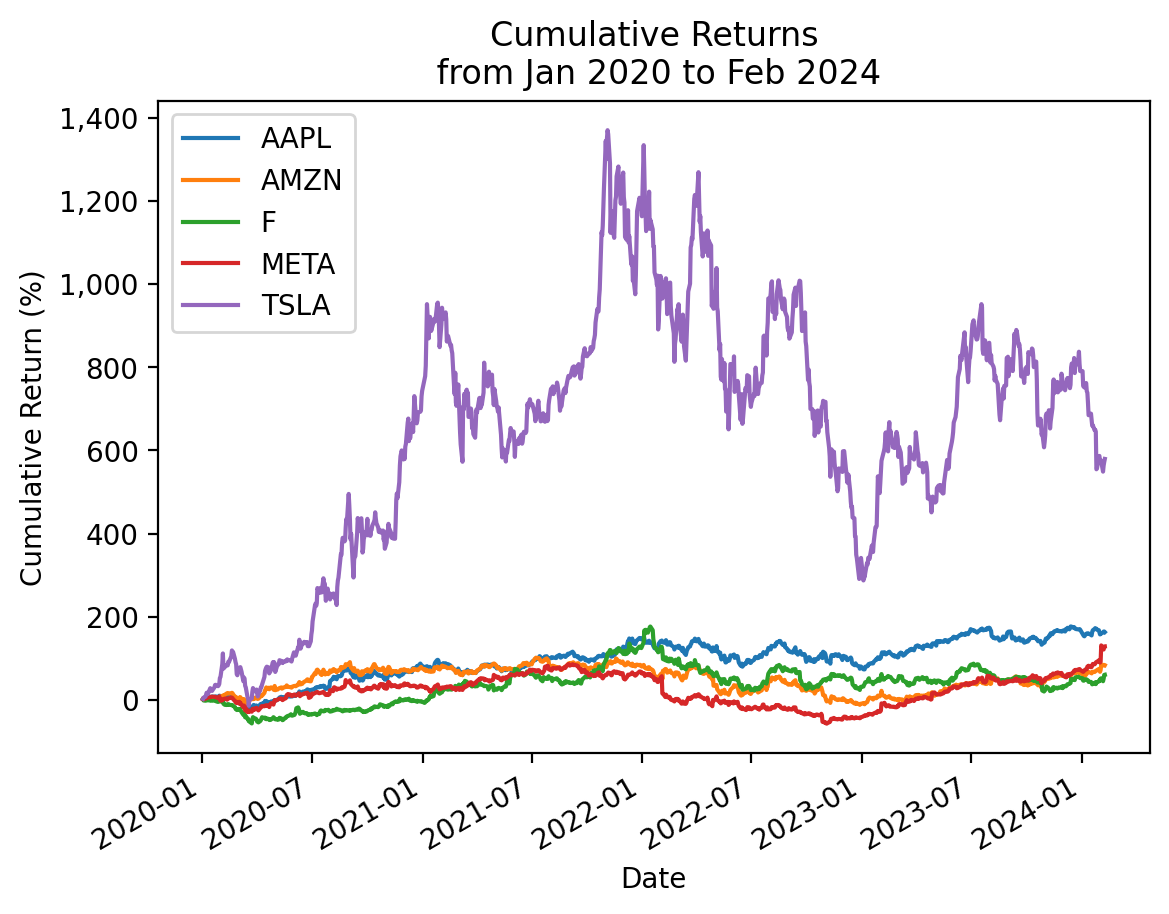
\includegraphics{herron_01_practice_02_files/figure-pdf/cell-19-output-1.png}

}

\end{figure}

\hypertarget{use-price-data-only-to-plot-cumulative-returns-for-these-stocks-in-the-2020s}{%
\subsection{Use price data only to plot cumulative returns for these
stocks in the
2020s}\label{use-price-data-only-to-plot-cumulative-returns-for-these-stocks-in-the-2020s}}

We can also calculate cumulative returns as the ratio of adjusted
closes. That is \(R_{0,T} = \frac{AC_T}{AC_0} - 1\). The trick here is
that \(FV_t = PV (1+r)^t\), so \((1+r)^t = \frac{FV_t}{PV}\).

\begin{Shaded}
\begin{Highlighting}[]
\NormalTok{returns\_2020s.iloc[}\DecValTok{0}\NormalTok{]}
\end{Highlighting}
\end{Shaded}

\begin{verbatim}
AAPL   0.0228
AMZN   0.0272
F      0.0129
META   0.0221
TSLA   0.0285
Name: 2020-01-02 00:00:00, dtype: float64
\end{verbatim}

\textbf{\emph{Note:}} We drop the last row in
\texttt{prices{[}\textquotesingle{}Adj\ Close\textquotesingle{}{]}} with
\texttt{.iloc{[}:-1{]}}. We drop this last row here here because we did
the same above when we calculated \texttt{returns} to exclude possible
intraday returns.

\begin{Shaded}
\begin{Highlighting}[]
\NormalTok{cumret\_prices }\OperatorTok{=}\NormalTok{ prices[}\StringTok{\textquotesingle{}Adj Close\textquotesingle{}}\NormalTok{].loc[}\StringTok{\textquotesingle{}2020\textquotesingle{}}\NormalTok{:].iloc[:}\OperatorTok{{-}}\DecValTok{1}\NormalTok{] }\OperatorTok{/}\NormalTok{ prices[}\StringTok{\textquotesingle{}Adj Close\textquotesingle{}}\NormalTok{].loc[}\StringTok{\textquotesingle{}2019\textquotesingle{}}\NormalTok{].iloc[}\OperatorTok{{-}}\DecValTok{1}\NormalTok{] }\OperatorTok{{-}} \DecValTok{1}

\NormalTok{cumret\_prices.iloc[}\DecValTok{0}\NormalTok{]}
\end{Highlighting}
\end{Shaded}

\begin{verbatim}
AAPL   0.0228
AMZN   0.0272
F      0.0129
META   0.0221
TSLA   0.0285
Name: 2020-01-02 00:00:00, dtype: float64
\end{verbatim}

\begin{Shaded}
\begin{Highlighting}[]
\NormalTok{np.allclose(cumret\_cumprod, cumret\_prices)}
\end{Highlighting}
\end{Shaded}

\begin{verbatim}
True
\end{verbatim}

\begin{Shaded}
\begin{Highlighting}[]
\NormalTok{cumret\_prices.mul(}\DecValTok{100}\NormalTok{).plot()}

\CommentTok{\# https://stackoverflow.com/questions/25973581/how{-}to{-}format{-}axis{-}number{-}format{-}to{-}thousands{-}with{-}a{-}comma}
\ImportTok{from}\NormalTok{ matplotlib }\ImportTok{import}\NormalTok{ ticker}
\NormalTok{plt.gca().get\_yaxis().set\_major\_formatter(ticker.FuncFormatter(}\KeywordTok{lambda}\NormalTok{ x, p: }\BuiltInTok{format}\NormalTok{(}\BuiltInTok{int}\NormalTok{(x), }\StringTok{\textquotesingle{},\textquotesingle{}}\NormalTok{)))}

\NormalTok{plt.ylabel(}\StringTok{\textquotesingle{}Cumulative Return (\%)\textquotesingle{}}\NormalTok{)}
\NormalTok{plt.title(}\SpecialStringTok{f\textquotesingle{}Cumulative Returns}\CharTok{\textbackslash{}n}\SpecialStringTok{ from }\SpecialCharTok{\{}\NormalTok{cumret\_prices}\SpecialCharTok{.}\NormalTok{index}\SpecialCharTok{.}\BuiltInTok{min}\NormalTok{()}\SpecialCharTok{:}\OperatorTok{\%}\NormalTok{b }\OperatorTok{\%}\NormalTok{Y}\SpecialCharTok{\}}\SpecialStringTok{ to }\SpecialCharTok{\{}\NormalTok{cumret\_prices}\SpecialCharTok{.}\NormalTok{index}\SpecialCharTok{.}\BuiltInTok{max}\NormalTok{()}\SpecialCharTok{:}\OperatorTok{\%}\NormalTok{b }\OperatorTok{\%}\NormalTok{Y}\SpecialCharTok{\}}\SpecialStringTok{\textquotesingle{}}\NormalTok{)}
\NormalTok{plt.show()}
\end{Highlighting}
\end{Shaded}

\begin{figure}[H]

{\centering 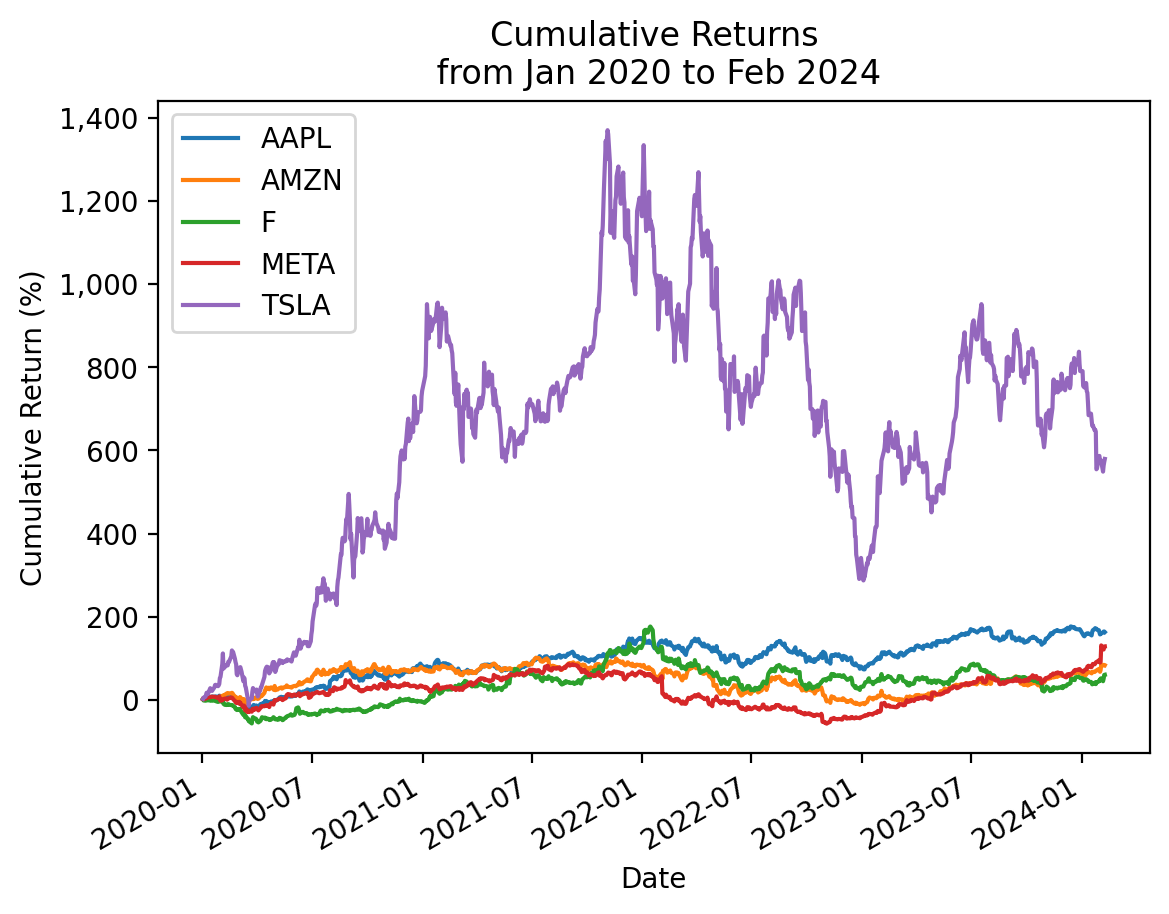
\includegraphics{herron_01_practice_02_files/figure-pdf/cell-23-output-1.png}

}

\end{figure}

\hypertarget{calculate-the-sharpe-ratio-for-tsla}{%
\subsection{Calculate the Sharpe Ratio for
TSLA}\label{calculate-the-sharpe-ratio-for-tsla}}

Calculate the Sharpe Ratio with all available returns and 2020s returns.
Recall the Sharpe Ratio is \(\frac{\overline{r_i - r_f}}{\sigma_i}\),
where \(\sigma_i\) is the volatility of \emph{excess} returns.

\textbf{\emph{I suggest you write a function named
\texttt{calc\_sharpe()} to use for the rest of this notebook.}}

\begin{Shaded}
\begin{Highlighting}[]
\KeywordTok{def}\NormalTok{ calc\_sharpe(ri, rf}\OperatorTok{=}\NormalTok{ff[}\StringTok{\textquotesingle{}RF\textquotesingle{}}\NormalTok{], ppy}\OperatorTok{=}\DecValTok{252}\NormalTok{):}
\NormalTok{    ri\_rf }\OperatorTok{=}\NormalTok{ ri.sub(rf).dropna()}
    \ControlFlowTok{return}\NormalTok{ np.sqrt(ppy) }\OperatorTok{*}\NormalTok{ ri\_rf.mean() }\OperatorTok{/}\NormalTok{ ri\_rf.std()}
\end{Highlighting}
\end{Shaded}

\begin{Shaded}
\begin{Highlighting}[]
\NormalTok{calc\_sharpe(ri}\OperatorTok{=}\NormalTok{returns[}\StringTok{\textquotesingle{}TSLA\textquotesingle{}}\NormalTok{])}
\end{Highlighting}
\end{Shaded}

\begin{verbatim}
0.9261
\end{verbatim}

\begin{Shaded}
\begin{Highlighting}[]
\NormalTok{calc\_sharpe(ri}\OperatorTok{=}\NormalTok{returns\_2020s[}\StringTok{\textquotesingle{}TSLA\textquotesingle{}}\NormalTok{])}
\end{Highlighting}
\end{Shaded}

\begin{verbatim}
1.1212
\end{verbatim}

We can use the \texttt{.pipe()} method here, too, since \texttt{ri} is
the first argument to \texttt{calc\_sharpe()}!

\begin{Shaded}
\begin{Highlighting}[]
\NormalTok{returns[}\StringTok{\textquotesingle{}TSLA\textquotesingle{}}\NormalTok{].pipe(calc\_sharpe)}
\end{Highlighting}
\end{Shaded}

\begin{verbatim}
0.9261
\end{verbatim}

\begin{Shaded}
\begin{Highlighting}[]
\NormalTok{returns\_2020s[}\StringTok{\textquotesingle{}TSLA\textquotesingle{}}\NormalTok{].pipe(calc\_sharpe)}
\end{Highlighting}
\end{Shaded}

\begin{verbatim}
1.1212
\end{verbatim}

\hypertarget{calculate-the-market-beta-for-tsla}{%
\subsection{Calculate the market beta for
TSLA}\label{calculate-the-market-beta-for-tsla}}

Calculate the market beta with all available returns and 2020s returns.
Recall we estimate market beta with the ordinary least squares (OLS)
regression \(R_i-R_f = \alpha + \beta (R_m-R_f) + \epsilon\). We can
estimate market beta with the covariance formula (i.e.,
\(\beta_i = \frac{Cov(R_i - R_f, R_m - R_f)}{Var(R_m-R_f)}\)) above for
a univariate regression if we do not need goodness of fit statistics.

\textbf{\emph{I suggest you write a function named \texttt{calc\_beta()}
to use for the rest of this notebook.}}

\begin{Shaded}
\begin{Highlighting}[]
\KeywordTok{def}\NormalTok{ calc\_beta(ri, rf}\OperatorTok{=}\NormalTok{ff[}\StringTok{\textquotesingle{}RF\textquotesingle{}}\NormalTok{], rm\_rf}\OperatorTok{=}\NormalTok{ff[}\StringTok{\textquotesingle{}Mkt{-}RF\textquotesingle{}}\NormalTok{]):}
\NormalTok{    ri\_rf }\OperatorTok{=}\NormalTok{ ri.sub(rf).dropna()}
\NormalTok{    rm\_rf }\OperatorTok{=}\NormalTok{ rm\_rf.loc[ri\_rf.index]}
    \ControlFlowTok{return}\NormalTok{ ri\_rf.cov(rm\_rf) }\OperatorTok{/}\NormalTok{ rm\_rf.var()}
\end{Highlighting}
\end{Shaded}

\begin{Shaded}
\begin{Highlighting}[]
\NormalTok{calc\_beta(ri}\OperatorTok{=}\NormalTok{returns[}\StringTok{\textquotesingle{}TSLA\textquotesingle{}}\NormalTok{])}
\end{Highlighting}
\end{Shaded}

\begin{verbatim}
1.4417
\end{verbatim}

\begin{Shaded}
\begin{Highlighting}[]
\NormalTok{calc\_beta(ri}\OperatorTok{=}\NormalTok{returns\_2020s[}\StringTok{\textquotesingle{}TSLA\textquotesingle{}}\NormalTok{])}
\end{Highlighting}
\end{Shaded}

\begin{verbatim}
1.5780
\end{verbatim}

We can use the \texttt{.pipe()} method here, too, since \texttt{ri} is
the first argument to \texttt{calc\_beta()}!

\begin{Shaded}
\begin{Highlighting}[]
\NormalTok{returns[}\StringTok{\textquotesingle{}TSLA\textquotesingle{}}\NormalTok{].pipe(calc\_beta)}
\end{Highlighting}
\end{Shaded}

\begin{verbatim}
1.4417
\end{verbatim}

\begin{Shaded}
\begin{Highlighting}[]
\NormalTok{returns\_2020s[}\StringTok{\textquotesingle{}TSLA\textquotesingle{}}\NormalTok{].pipe(calc\_beta)}
\end{Highlighting}
\end{Shaded}

\begin{verbatim}
1.5780
\end{verbatim}

\hypertarget{guess-the-sharpe-ratios-for-these-stocks-in-the-2020s}{%
\subsection{Guess the Sharpe Ratios for these stocks in the
2020s}\label{guess-the-sharpe-ratios-for-these-stocks-in-the-2020s}}

\hypertarget{guess-the-market-betas-for-these-stocks-in-the-2020s}{%
\subsection{Guess the market betas for these stocks in the
2020s}\label{guess-the-market-betas-for-these-stocks-in-the-2020s}}

\hypertarget{calculate-the-sharpe-ratios-for-these-stocks-in-the-2020s}{%
\subsection{Calculate the Sharpe Ratios for these stocks in the
2020s}\label{calculate-the-sharpe-ratios-for-these-stocks-in-the-2020s}}

How good were your guesses?

\begin{Shaded}
\begin{Highlighting}[]
\ControlFlowTok{for}\NormalTok{ i }\KeywordTok{in}\NormalTok{ returns\_2020s:}
\NormalTok{    sharpe\_i }\OperatorTok{=}\NormalTok{ returns\_2020s[i].pipe(calc\_sharpe)}
    \BuiltInTok{print}\NormalTok{(}\SpecialStringTok{f\textquotesingle{}Sharpe Ratio for }\SpecialCharTok{\{}\NormalTok{i}\SpecialCharTok{\}}\SpecialStringTok{:}\CharTok{\textbackslash{}t}\SpecialStringTok{ }\SpecialCharTok{\{}\NormalTok{sharpe\_i}\SpecialCharTok{:0.2f\}}\SpecialStringTok{\textquotesingle{}}\NormalTok{)}
\end{Highlighting}
\end{Shaded}

\begin{verbatim}
Sharpe Ratio for AAPL:   0.86
Sharpe Ratio for AMZN:   0.48
Sharpe Ratio for F:  0.42
Sharpe Ratio for META:   0.49
Sharpe Ratio for TSLA:   1.12
\end{verbatim}

We can also use pandas notation to vectorize this calculation. First
calculate \emph{excess} returns as \(r_i - r_f\).

\begin{Shaded}
\begin{Highlighting}[]
\NormalTok{returns\_2020s\_excess }\OperatorTok{=}\NormalTok{ returns\_2020s.sub(ff[}\StringTok{\textquotesingle{}RF\textquotesingle{}}\NormalTok{], axis}\OperatorTok{=}\DecValTok{0}\NormalTok{).dropna()}
\end{Highlighting}
\end{Shaded}

Then use pandas notation to calculate means, standard deviations, and
annualize.

\begin{Shaded}
\begin{Highlighting}[]
\NormalTok{(}
\NormalTok{    returns\_2020s\_excess}
\NormalTok{    .mean()}
\NormalTok{    .div(returns\_2020s\_excess.std())}
\NormalTok{    .mul(np.sqrt(}\DecValTok{252}\NormalTok{))}
\NormalTok{)}
\end{Highlighting}
\end{Shaded}

\begin{verbatim}
AAPL   0.8576
AMZN   0.4750
F      0.4240
META   0.4949
TSLA   1.1212
dtype: float64
\end{verbatim}

\textbf{\emph{Note:}} In a few weeks we will learn the \texttt{.apply()}
method, which avoids the loop syntax.

\begin{Shaded}
\begin{Highlighting}[]
\NormalTok{returns\_2020s.}\BuiltInTok{apply}\NormalTok{(calc\_sharpe)}
\end{Highlighting}
\end{Shaded}

\begin{verbatim}
AAPL   0.8576
AMZN   0.4750
F      0.4240
META   0.4949
TSLA   1.1212
dtype: float64
\end{verbatim}

\hypertarget{calculate-the-market-betas-for-these-stocks-in-the-2020s}{%
\subsection{Calculate the market betas for these stocks in the
2020s}\label{calculate-the-market-betas-for-these-stocks-in-the-2020s}}

How good were your guesses?

\begin{Shaded}
\begin{Highlighting}[]
\ControlFlowTok{for}\NormalTok{ i }\KeywordTok{in}\NormalTok{ returns\_2020s:}
\NormalTok{    beta\_i }\OperatorTok{=}\NormalTok{ returns\_2020s[i].pipe(calc\_beta)}
    \BuiltInTok{print}\NormalTok{(}\SpecialStringTok{f\textquotesingle{}Beta for }\SpecialCharTok{\{}\NormalTok{i}\SpecialCharTok{\}}\SpecialStringTok{:}\CharTok{\textbackslash{}t}\SpecialStringTok{ }\SpecialCharTok{\{}\NormalTok{beta\_i}\SpecialCharTok{:0.2f\}}\SpecialStringTok{\textquotesingle{}}\NormalTok{)}
\end{Highlighting}
\end{Shaded}

\begin{verbatim}
Beta for AAPL:   1.15
Beta for AMZN:   1.04
Beta for F:  1.22
Beta for META:   1.27
Beta for TSLA:   1.58
\end{verbatim}

Or we can follow out approach above to vectorize this calculation.
First, we need to add a market excess return column to
\texttt{returns\_2020s\_excess}.

\begin{Shaded}
\begin{Highlighting}[]
\NormalTok{returns\_2020s\_excess[}\StringTok{\textquotesingle{}Mkt{-}RF\textquotesingle{}}\NormalTok{] }\OperatorTok{=}\NormalTok{ ff[}\StringTok{\textquotesingle{}Mkt{-}RF\textquotesingle{}}\NormalTok{]}
\NormalTok{returns\_2020s\_excess.head()}
\end{Highlighting}
\end{Shaded}

\begin{longtable}[]{@{}lllllll@{}}
\toprule\noalign{}
& AAPL & AMZN & F & META & TSLA & Mkt-RF \\
Date & & & & & & \\
\midrule\noalign{}
\endhead
\bottomrule\noalign{}
\endlastfoot
2020-01-02 & 0.0228 & 0.0271 & 0.0128 & 0.0220 & 0.0285 & 0.0086 \\
2020-01-03 & -0.0098 & -0.0122 & -0.0224 & -0.0054 & 0.0296 & -0.0067 \\
2020-01-06 & 0.0079 & 0.0148 & -0.0055 & 0.0188 & 0.0192 & 0.0036 \\
2020-01-07 & -0.0048 & 0.0020 & 0.0098 & 0.0021 & 0.0387 & -0.0019 \\
2020-01-08 & 0.0160 & -0.0079 & -0.0001 & 0.0101 & 0.0491 & 0.0047 \\
\end{longtable}

\begin{Shaded}
\begin{Highlighting}[]
\NormalTok{vcv }\OperatorTok{=}\NormalTok{ returns\_2020s\_excess.cov()}
\NormalTok{vcv}
\end{Highlighting}
\end{Shaded}

\begin{longtable}[]{@{}lllllll@{}}
\toprule\noalign{}
& AAPL & AMZN & F & META & TSLA & Mkt-RF \\
\midrule\noalign{}
\endhead
\bottomrule\noalign{}
\endlastfoot
AAPL & 0.0004 & 0.0003 & 0.0002 & 0.0004 & 0.0005 & 0.0003 \\
AMZN & 0.0003 & 0.0006 & 0.0002 & 0.0004 & 0.0005 & 0.0002 \\
F & 0.0002 & 0.0002 & 0.0009 & 0.0003 & 0.0005 & 0.0003 \\
META & 0.0004 & 0.0004 & 0.0003 & 0.0009 & 0.0005 & 0.0003 \\
TSLA & 0.0005 & 0.0005 & 0.0005 & 0.0005 & 0.0018 & 0.0003 \\
Mkt-RF & 0.0003 & 0.0002 & 0.0003 & 0.0003 & 0.0003 & 0.0002 \\
\end{longtable}

\begin{Shaded}
\begin{Highlighting}[]
\NormalTok{vcv[}\StringTok{\textquotesingle{}Mkt{-}RF\textquotesingle{}}\NormalTok{].div(vcv.loc[}\StringTok{\textquotesingle{}Mkt{-}RF\textquotesingle{}}\NormalTok{, }\StringTok{\textquotesingle{}Mkt{-}RF\textquotesingle{}}\NormalTok{]).plot(kind}\OperatorTok{=}\StringTok{\textquotesingle{}bar\textquotesingle{}}\NormalTok{)}
\NormalTok{plt.xlabel(}\StringTok{\textquotesingle{}Ticker\textquotesingle{}}\NormalTok{)}
\NormalTok{plt.ylabel(}\StringTok{\textquotesingle{}CAPM Beta\textquotesingle{}}\NormalTok{)}
\NormalTok{plt.title(}\StringTok{\textquotesingle{}CAPM Betas\textquotesingle{}}\NormalTok{)}
\NormalTok{plt.show()}
\end{Highlighting}
\end{Shaded}

\begin{figure}[H]

{\centering 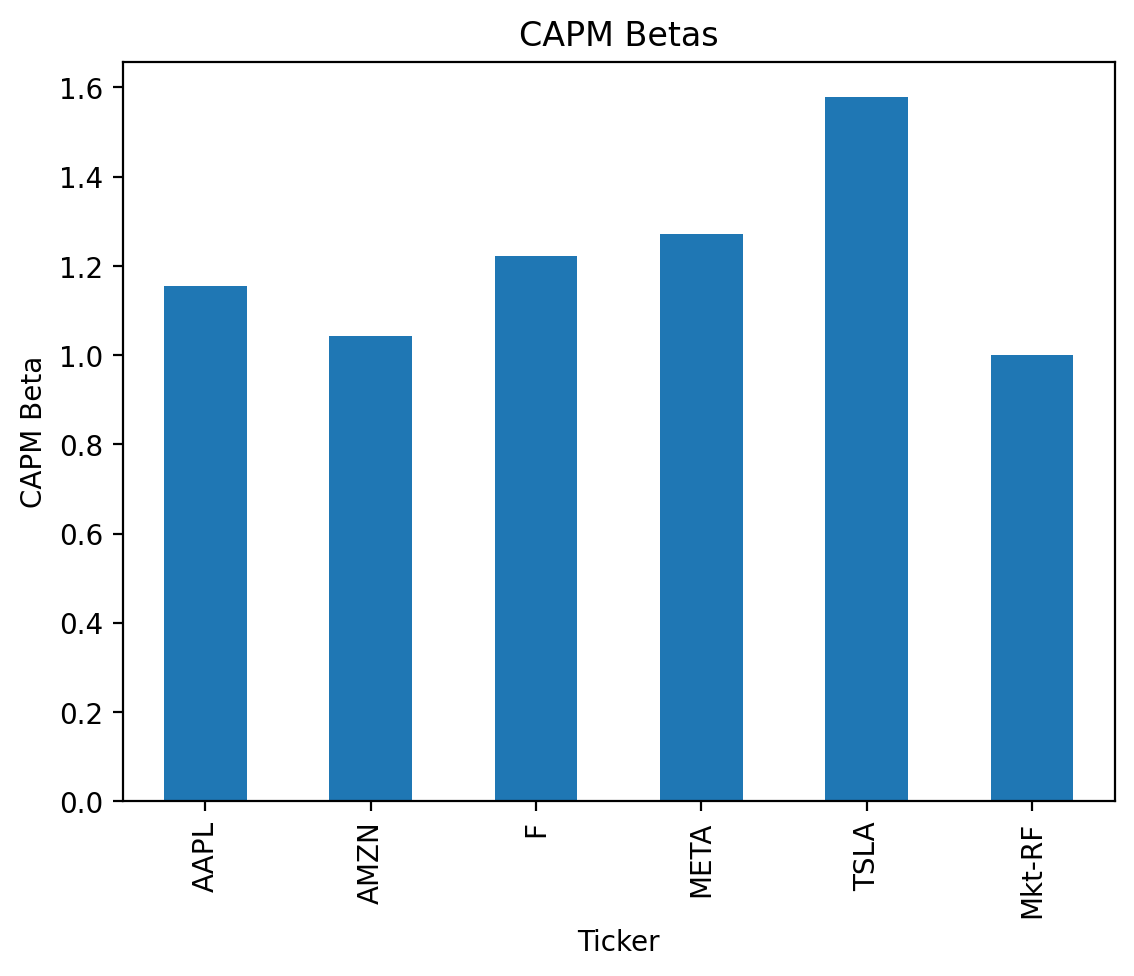
\includegraphics{herron_01_practice_02_files/figure-pdf/cell-41-output-1.png}

}

\end{figure}

\textbf{\emph{Note:}} In a few weeks we will learn the \texttt{.apply()}
method, which avoids the loop syntax.

\begin{Shaded}
\begin{Highlighting}[]
\NormalTok{returns\_2020s.}\BuiltInTok{apply}\NormalTok{(calc\_beta)}
\end{Highlighting}
\end{Shaded}

\begin{verbatim}
AAPL   1.1541
AMZN   1.0429
F      1.2231
META   1.2710
TSLA   1.5780
dtype: float64
\end{verbatim}

\hypertarget{calculate-the-sharpe-ratio-for-an-equally-weighted-portfolio-of-these-stocks-in-the-2020s}{%
\subsection{\texorpdfstring{Calculate the Sharpe Ratio for an
\emph{equally weighted} portfolio of these stocks in the
2020s}{Calculate the Sharpe Ratio for an equally weighted portfolio of these stocks in the 2020s}}\label{calculate-the-sharpe-ratio-for-an-equally-weighted-portfolio-of-these-stocks-in-the-2020s}}

What do you notice?

\begin{Shaded}
\begin{Highlighting}[]
\NormalTok{returns\_2020s.mean(axis}\OperatorTok{=}\DecValTok{1}\NormalTok{).pipe(calc\_sharpe)}
\end{Highlighting}
\end{Shaded}

\begin{verbatim}
0.9573
\end{verbatim}

Because diversification reduces portfolio standard deviation less than
the sum of its parts, the Sharpe Ratio of the equally weighted portfolio
is less than the equally weighted mean of the single-stock Sharpe
Ratios.

\begin{Shaded}
\begin{Highlighting}[]
\NormalTok{returns\_2020s.}\BuiltInTok{apply}\NormalTok{(calc\_sharpe).mean()}
\end{Highlighting}
\end{Shaded}

\begin{verbatim}
0.6745
\end{verbatim}

\hypertarget{calculate-the-market-beta-for-an-equally-weighted-portfolio-of-these-stocks-in-the-2020s}{%
\subsection{\texorpdfstring{Calculate the market beta for an
\emph{equally weighted} portfolio of these stocks in the
2020s}{Calculate the market beta for an equally weighted portfolio of these stocks in the 2020s}}\label{calculate-the-market-beta-for-an-equally-weighted-portfolio-of-these-stocks-in-the-2020s}}

What do you notice?

Beta measures \emph{non}diversifiable risk, so
\(\beta_P = \sum w_i \beta_i\)!

\begin{Shaded}
\begin{Highlighting}[]
\NormalTok{returns\_2020s.mean(axis}\OperatorTok{=}\DecValTok{1}\NormalTok{).pipe(calc\_beta)}
\end{Highlighting}
\end{Shaded}

\begin{verbatim}
1.2538
\end{verbatim}

\begin{Shaded}
\begin{Highlighting}[]
\NormalTok{returns\_2020s.}\BuiltInTok{apply}\NormalTok{(calc\_beta).mean()}
\end{Highlighting}
\end{Shaded}

\begin{verbatim}
1.2538
\end{verbatim}

\hypertarget{calculate-the-market-betas-for-these-stocks-every-calendar-year-for-every-possible-year}{%
\subsection{Calculate the market betas for these stocks every calendar
year for every possible
year}\label{calculate-the-market-betas-for-these-stocks-every-calendar-year-for-every-possible-year}}

Save these market betas to data frame \texttt{betas}. Our current Python
knowledge limits us to a for-loop, but we will learn easier and faster
approaches soon!

\begin{Shaded}
\begin{Highlighting}[]
\NormalTok{betas }\OperatorTok{=}\NormalTok{ pd.DataFrame(}
\NormalTok{    index}\OperatorTok{=}\BuiltInTok{range}\NormalTok{(}\DecValTok{1972}\NormalTok{, }\DecValTok{2024}\NormalTok{),}
\NormalTok{    columns}\OperatorTok{=}\NormalTok{returns.columns}
\NormalTok{)}

\NormalTok{betas.columns.name }\OperatorTok{=} \StringTok{\textquotesingle{}Ticker\textquotesingle{}}
\NormalTok{betas.index.name }\OperatorTok{=} \StringTok{\textquotesingle{}Year\textquotesingle{}}

\NormalTok{betas.tail()}
\end{Highlighting}
\end{Shaded}

\begin{longtable}[]{@{}llllll@{}}
\toprule\noalign{}
Ticker & AAPL & AMZN & F & META & TSLA \\
Year & & & & & \\
\midrule\noalign{}
\endhead
\bottomrule\noalign{}
\endlastfoot
2019 & NaN & NaN & NaN & NaN & NaN \\
2020 & NaN & NaN & NaN & NaN & NaN \\
2021 & NaN & NaN & NaN & NaN & NaN \\
2022 & NaN & NaN & NaN & NaN & NaN \\
2023 & NaN & NaN & NaN & NaN & NaN \\
\end{longtable}

\begin{Shaded}
\begin{Highlighting}[]
\ControlFlowTok{for}\NormalTok{ i }\KeywordTok{in}\NormalTok{ betas.index: }
    \ControlFlowTok{for}\NormalTok{ c }\KeywordTok{in}\NormalTok{ betas.columns:}
\NormalTok{        betas.at[i, c] }\OperatorTok{=}\NormalTok{ returns.loc[}\BuiltInTok{str}\NormalTok{(i), c].pipe(calc\_beta)}

\NormalTok{betas.tail()}
\end{Highlighting}
\end{Shaded}

\begin{longtable}[]{@{}llllll@{}}
\toprule\noalign{}
Ticker & AAPL & AMZN & F & META & TSLA \\
Year & & & & & \\
\midrule\noalign{}
\endhead
\bottomrule\noalign{}
\endlastfoot
2019 & 1.4751 & 1.2752 & 1.0733 & 1.2094 & 1.3262 \\
2020 & 1.1174 & 0.6866 & 1.1052 & 0.9913 & 1.3041 \\
2021 & 1.1957 & 0.9822 & 1.2396 & 1.2014 & 1.9891 \\
2022 & 1.2386 & 1.5922 & 1.3824 & 1.6843 & 1.7414 \\
2023 & 1.0369 & 1.4649 & 1.3947 & 1.6630 & 2.2218 \\
\end{longtable}

\hypertarget{plot-the-time-series-of-market-betas}{%
\subsection{Plot the time series of market
betas}\label{plot-the-time-series-of-market-betas}}

\begin{Shaded}
\begin{Highlighting}[]
\NormalTok{betas.plot()}
\NormalTok{plt.ylabel(}\StringTok{\textquotesingle{}CAPM Beta\textquotesingle{}}\NormalTok{)}
\NormalTok{plt.title(}\StringTok{\textquotesingle{}CAPM Betas\textquotesingle{}}\NormalTok{)}
\NormalTok{plt.show()}
\end{Highlighting}
\end{Shaded}

\begin{figure}[H]

{\centering 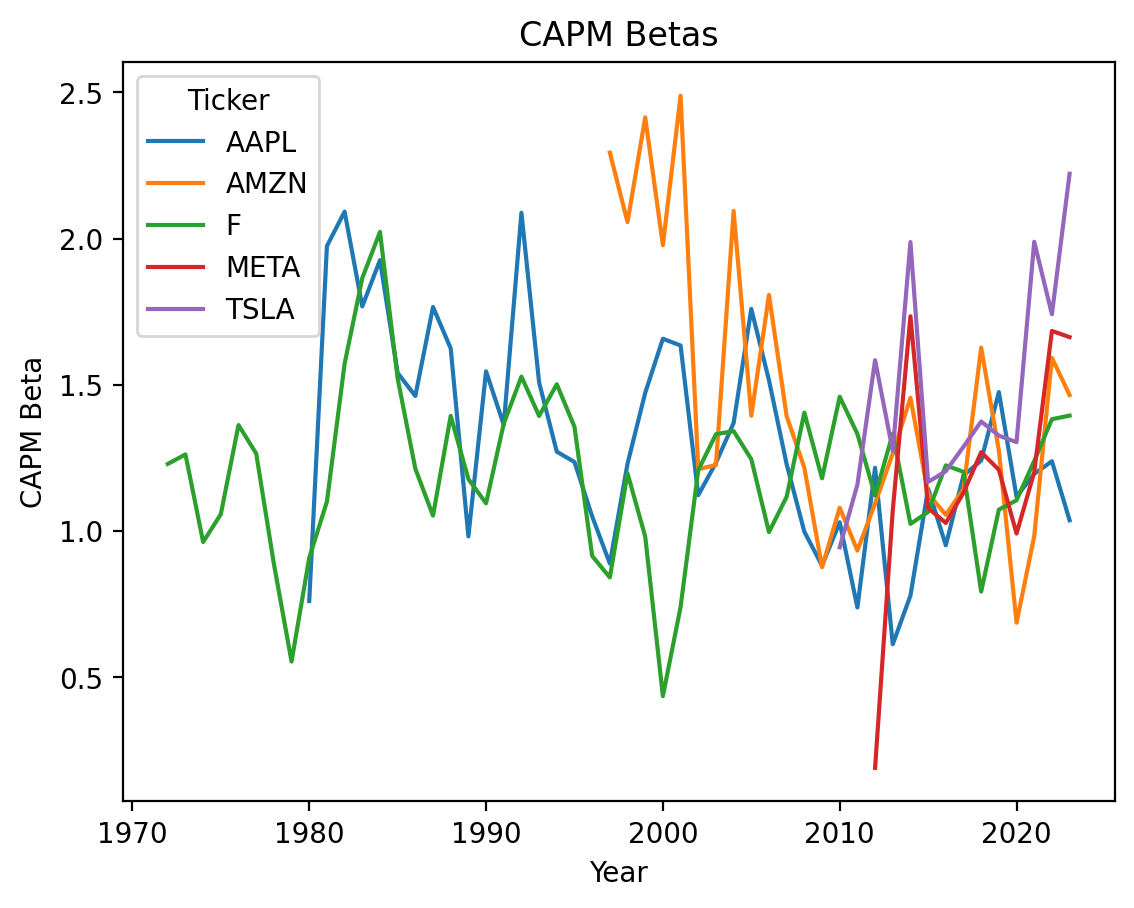
\includegraphics{herron_01_practice_02_files/figure-pdf/cell-49-output-1.png}

}

\end{figure}

\hypertarget{herron-topic-1---practice-for-section-03}{%
\chapter{Herron Topic 1 - Practice for Section
03}\label{herron-topic-1---practice-for-section-03}}

\hypertarget{announcements-17}{%
\section{Announcements}\label{announcements-17}}

\begin{enumerate}
\def\labelenumi{\arabic{enumi}.}
\tightlist
\item
  DataCamp

  \begin{enumerate}
  \def\labelenumii{\arabic{enumii}.}
  \tightlist
  \item
    \emph{Data Manipulation with pandas} due by Friday, 2/9, at 11:59 PM
  \item
    \emph{Joining Data with pandas} due by Friday, 2/16, at 11:59 PM
  \item
    \emph{Earn 10,000 XP} due by Friday, 3/15, at 11:59 PM
  \end{enumerate}
\item
  I posted Project 1 to Canvas

  \begin{enumerate}
  \def\labelenumii{\arabic{enumii}.}
  \tightlist
  \item
    Slides and notebook due by Friday, 2/23, at 11:59 PM
  \item
    Keep joining teams and let me know if you need help
  \end{enumerate}
\end{enumerate}

\hypertarget{minute-recap-16}{%
\section{10-Minute Recap}\label{minute-recap-16}}

\begin{Shaded}
\begin{Highlighting}[]
\ImportTok{import}\NormalTok{ matplotlib.pyplot }\ImportTok{as}\NormalTok{ plt}
\ImportTok{import}\NormalTok{ numpy }\ImportTok{as}\NormalTok{ np}
\ImportTok{import}\NormalTok{ pandas }\ImportTok{as}\NormalTok{ pd}
\ImportTok{import}\NormalTok{ pandas\_datareader }\ImportTok{as}\NormalTok{ pdr}
\ImportTok{import}\NormalTok{ yfinance }\ImportTok{as}\NormalTok{ yf}
\end{Highlighting}
\end{Shaded}

\begin{Shaded}
\begin{Highlighting}[]
\OperatorTok{\%}\NormalTok{precision }\DecValTok{4}
\NormalTok{pd.options.display.float\_format }\OperatorTok{=} \StringTok{\textquotesingle{}}\SpecialCharTok{\{:.4f\}}\StringTok{\textquotesingle{}}\NormalTok{.}\BuiltInTok{format}
\OperatorTok{\%}\NormalTok{config InlineBackend.figure\_format }\OperatorTok{=} \StringTok{\textquotesingle{}retina\textquotesingle{}}
\end{Highlighting}
\end{Shaded}

First, we can easily download data in Python with two packages:

\begin{enumerate}
\def\labelenumi{\arabic{enumi}.}
\tightlist
\item
  \texttt{yfinance} to download data from Yahoo! Finance
\item
  \texttt{pandas-datareader} to download data from Ken French (and FRED
  and others)
\end{enumerate}

Second, there are ``simple returns'' and ``log returns''

\begin{enumerate}
\def\labelenumi{\arabic{enumi}.}
\tightlist
\item
  Simple returns are the returns that investors receive that we learned
  in FINA 6331 and FINA 6333:
  \(r_t = \frac{p_t + d_t - p_{t-1}}{p_{t-1}}\)
\item
  Log returns are the log of one plus simple returns. Why do we use
  them?

  \begin{enumerate}
  \def\labelenumii{\arabic{enumii}.}
  \tightlist
  \item
    \textbf{\emph{Log returns are additive}}, while simple returns are
    multiplicative. This additive property makes math really easy with
    log returns:
    \(\log(\prod_{t=0}^T (1 + r_t)) = \sum_{t=0}^T \log(1+r_t)\), so
    \(r_{0,T} = \prod_{t=0}^T (1 + r_t) - 1 = e^{\sum_{t=0}^T \log(1+r_t)} - 1\)
  \item
    \textbf{\emph{Log returns are almost normally distributed}}
  \end{enumerate}
\end{enumerate}

\textbf{\emph{We will almost always use simple returns.}} The exeception
is time-consuming calculations, which we will often do in log returns to
save us time.

Third, we can easily calculate portfolio returns in pandas!

\begin{enumerate}
\def\labelenumi{\arabic{enumi}.}
\tightlist
\item
  \texttt{returns.mean(axis=1)} is the equally-weighted portfolio return
  for the stocks in \texttt{returns}, \textbf{\emph{rebalanced at the
  same frequency as the returns in \texttt{returns}!}}
\item
  \texttt{returns.dot(weights)} lets us use weights in array
  \texttt{weights} instead of equally-weighted, but is still
  \textbf{\emph{rebalanced at the same frequency as the returns in
  \texttt{returns}!}}
\end{enumerate}

\hypertarget{practice-17}{%
\section{Practice}\label{practice-17}}

\hypertarget{download-all-available-daily-price-data-for-tickers-tsla-f-aapl-amzn-and-meta-to-data-frame-prices-1}{%
\subsection{\texorpdfstring{Download all available daily price data for
tickers TSLA, F, AAPL, AMZN, and META to data frame
\texttt{prices}}{Download all available daily price data for tickers TSLA, F, AAPL, AMZN, and META to data frame prices}}\label{download-all-available-daily-price-data-for-tickers-tsla-f-aapl-amzn-and-meta-to-data-frame-prices-1}}

\begin{Shaded}
\begin{Highlighting}[]
\NormalTok{tickers }\OperatorTok{=} \StringTok{\textquotesingle{}TSLA F AAPL AMZN META\textquotesingle{}}
\NormalTok{prices }\OperatorTok{=}\NormalTok{ yf.download(tickers}\OperatorTok{=}\NormalTok{tickers)}

\NormalTok{prices}
\end{Highlighting}
\end{Shaded}

\begin{verbatim}
[*********************100%%**********************]  5 of 5 completed
\end{verbatim}

\begin{longtable}[]{@{}llllllllllllllllllllll@{}}
\toprule\noalign{}
&
\multicolumn{5}{>{\raggedright\arraybackslash}p{(\columnwidth - 42\tabcolsep) * \real{0.0000} + 8\tabcolsep}}{%
Adj Close} &
\multicolumn{5}{>{\raggedright\arraybackslash}p{(\columnwidth - 42\tabcolsep) * \real{0.0000} + 8\tabcolsep}}{%
Close} & ... &
\multicolumn{5}{>{\raggedright\arraybackslash}p{(\columnwidth - 42\tabcolsep) * \real{0.0000} + 8\tabcolsep}}{%
Open} &
\multicolumn{5}{>{\raggedright\arraybackslash}p{(\columnwidth - 42\tabcolsep) * \real{0.0000} + 8\tabcolsep}@{}}{%
Volume} \\
& AAPL & AMZN & F & META & TSLA & AAPL & AMZN & F & META & TSLA & ... &
AAPL & AMZN & F & META & TSLA & AAPL & AMZN & F & META & TSLA \\
Date & & & & & & & & & & & & & & & & & & & & & \\
\midrule\noalign{}
\endhead
\bottomrule\noalign{}
\endlastfoot
1972-06-01 & NaN & NaN & 0.2419 & NaN & NaN & NaN & NaN & 2.1532 & NaN &
NaN & ... & NaN & NaN & 0.0000 & NaN & NaN & NaN & NaN & 1091238 & NaN &
NaN \\
1972-06-02 & NaN & NaN & 0.2414 & NaN & NaN & NaN & NaN & 2.1492 & NaN &
NaN & ... & NaN & NaN & 2.1532 & NaN & NaN & NaN & NaN & 1174468 & NaN &
NaN \\
1972-06-05 & NaN & NaN & 0.2414 & NaN & NaN & NaN & NaN & 2.1492 & NaN &
NaN & ... & NaN & NaN & 2.1492 & NaN & NaN & NaN & NaN & 5209582 & NaN &
NaN \\
1972-06-06 & NaN & NaN & 0.2387 & NaN & NaN & NaN & NaN & 2.1248 & NaN &
NaN & ... & NaN & NaN & 2.1492 & NaN & NaN & NaN & NaN & 1424158 & NaN &
NaN \\
1972-06-07 & NaN & NaN & 0.2373 & NaN & NaN & NaN & NaN & 2.1127 & NaN &
NaN & ... & NaN & NaN & 2.1248 & NaN & NaN & NaN & NaN & 675088 & NaN &
NaN \\
... & ... & ... & ... & ... & ... & ... & ... & ... & ... & ... & ... &
... & ... & ... & ... & ... & ... & ... & ... & ... & ... \\
2024-02-05 & 187.6800 & 170.3100 & 11.5900 & 459.4100 & 181.0600 &
187.6800 & 170.3100 & 11.5900 & 459.4100 & 181.0600 & ... & 188.1500 &
170.2000 & 12.0100 & 469.8800 & 184.2600 & 69668800.0000 & 55081300.0000
& 81026800 & 40832400.0000 & 134294400.0000 \\
2024-02-06 & 189.3000 & 169.1500 & 12.0700 & 454.7200 & 185.1000 &
189.3000 & 169.1500 & 12.0700 & 454.7200 & 185.1000 & ... & 186.8600 &
169.3900 & 11.6400 & 464.0000 & 177.2100 & 43490800.0000 & 42505500.0000
& 98636800 & 21655200.0000 & 122676000.0000 \\
2024-02-07 & 189.4100 & 170.5300 & 12.8000 & 469.5900 & 187.5800 &
189.4100 & 170.5300 & 12.8000 & 469.5900 & 187.5800 & ... & 190.6400 &
169.4800 & 12.7300 & 458.0000 & 188.1800 & 53439000.0000 & 47174100.0000
& 137224000 & 23066000.0000 & 111535200.0000 \\
2024-02-08 & 188.3200 & 169.8400 & 12.8300 & 470.0000 & 189.5600 &
188.3200 & 169.8400 & 12.8300 & 470.0000 & 189.5600 & ... & 189.3900 &
169.6500 & 12.8700 & 468.3200 & 189.0000 & 40962000.0000 & 42316500.0000
& 68653900 & 18815100.0000 & 83034000.0000 \\
2024-02-09 & 188.8500 & 174.4500 & 12.6800 & 468.1100 & 193.5700 &
188.8500 & 174.4500 & 12.6800 & 468.1100 & 193.5700 & ... & 188.6500 &
170.9000 & 12.8100 & 472.9500 & 190.1800 & 43728065.0000 & 56886544.0000
& 46925766 & 18159624.0000 & 84009121.0000 \\
\end{longtable}

\hypertarget{calculate-all-available-daily-returns-and-save-to-data-frame-returns-1}{%
\subsection{\texorpdfstring{Calculate all available daily returns and
save to data frame
\texttt{returns}}{Calculate all available daily returns and save to data frame returns}}\label{calculate-all-available-daily-returns-and-save-to-data-frame-returns-1}}

\begin{Shaded}
\begin{Highlighting}[]
\NormalTok{returns }\OperatorTok{=}\NormalTok{ (}
\NormalTok{    prices[}\StringTok{\textquotesingle{}Adj Close\textquotesingle{}}\NormalTok{] }\CommentTok{\# slice adj close}
\NormalTok{    .iloc[:}\OperatorTok{{-}}\DecValTok{1}\NormalTok{] }\CommentTok{\# drop the last price because it might be intraday (i.e., not a close)}
\NormalTok{    .pct\_change() }\CommentTok{\# calculate simple returns}
\NormalTok{)}

\NormalTok{returns}
\end{Highlighting}
\end{Shaded}

\begin{longtable}[]{@{}llllll@{}}
\toprule\noalign{}
& AAPL & AMZN & F & META & TSLA \\
Date & & & & & \\
\midrule\noalign{}
\endhead
\bottomrule\noalign{}
\endlastfoot
1972-06-01 & NaN & NaN & NaN & NaN & NaN \\
1972-06-02 & NaN & NaN & -0.0019 & NaN & NaN \\
1972-06-05 & NaN & NaN & 0.0000 & NaN & NaN \\
1972-06-06 & NaN & NaN & -0.0113 & NaN & NaN \\
1972-06-07 & NaN & NaN & -0.0057 & NaN & NaN \\
... & ... & ... & ... & ... & ... \\
2024-02-02 & -0.0054 & 0.0787 & 0.0033 & 0.2032 & -0.0050 \\
2024-02-05 & 0.0098 & -0.0087 & -0.0453 & -0.0328 & -0.0365 \\
2024-02-06 & 0.0086 & -0.0068 & 0.0414 & -0.0102 & 0.0223 \\
2024-02-07 & 0.0006 & 0.0082 & 0.0605 & 0.0327 & 0.0134 \\
2024-02-08 & -0.0058 & -0.0040 & 0.0023 & 0.0009 & 0.0106 \\
\end{longtable}

\hypertarget{slices-returns-for-the-2020s-and-assign-to-returns_2020s-1}{%
\subsection{\texorpdfstring{Slices returns for the 2020s and assign to
\texttt{returns\_2020s}}{Slices returns for the 2020s and assign to returns\_2020s}}\label{slices-returns-for-the-2020s-and-assign-to-returns_2020s-1}}

\begin{Shaded}
\begin{Highlighting}[]
\NormalTok{returns\_2020s }\OperatorTok{=}\NormalTok{ returns.loc[}\StringTok{\textquotesingle{}2020\textquotesingle{}}\NormalTok{:] }\CommentTok{\# always use an unambiguos date format, like YYYY{-}MM{-}DD}

\NormalTok{returns\_2020s}
\end{Highlighting}
\end{Shaded}

\begin{longtable}[]{@{}llllll@{}}
\toprule\noalign{}
& AAPL & AMZN & F & META & TSLA \\
Date & & & & & \\
\midrule\noalign{}
\endhead
\bottomrule\noalign{}
\endlastfoot
2020-01-02 & 0.0228 & 0.0272 & 0.0129 & 0.0221 & 0.0285 \\
2020-01-03 & -0.0097 & -0.0121 & -0.0223 & -0.0053 & 0.0296 \\
2020-01-06 & 0.0080 & 0.0149 & -0.0054 & 0.0188 & 0.0193 \\
2020-01-07 & -0.0047 & 0.0021 & 0.0098 & 0.0022 & 0.0388 \\
2020-01-08 & 0.0161 & -0.0078 & 0.0000 & 0.0101 & 0.0492 \\
... & ... & ... & ... & ... & ... \\
2024-02-02 & -0.0054 & 0.0787 & 0.0033 & 0.2032 & -0.0050 \\
2024-02-05 & 0.0098 & -0.0087 & -0.0453 & -0.0328 & -0.0365 \\
2024-02-06 & 0.0086 & -0.0068 & 0.0414 & -0.0102 & 0.0223 \\
2024-02-07 & 0.0006 & 0.0082 & 0.0605 & 0.0327 & 0.0134 \\
2024-02-08 & -0.0058 & -0.0040 & 0.0023 & 0.0009 & 0.0106 \\
\end{longtable}

\hypertarget{download-all-available-data-for-the-fama-and-french-daily-benchmark-factors-to-dictionary-ff_all-1}{%
\subsection{\texorpdfstring{Download all available data for the Fama and
French daily benchmark factors to dictionary
\texttt{ff\_all}}{Download all available data for the Fama and French daily benchmark factors to dictionary ff\_all}}\label{download-all-available-data-for-the-fama-and-french-daily-benchmark-factors-to-dictionary-ff_all-1}}

I often use the following code snippet to find the exact name for the
the daily benchmark factors file.

\begin{Shaded}
\begin{Highlighting}[]
\NormalTok{pdr.famafrench.get\_available\_datasets()[:}\DecValTok{5}\NormalTok{]}
\end{Highlighting}
\end{Shaded}

\begin{verbatim}
['F-F_Research_Data_Factors',
 'F-F_Research_Data_Factors_weekly',
 'F-F_Research_Data_Factors_daily',
 'F-F_Research_Data_5_Factors_2x3',
 'F-F_Research_Data_5_Factors_2x3_daily']
\end{verbatim}

\begin{Shaded}
\begin{Highlighting}[]
\NormalTok{ff\_all }\OperatorTok{=}\NormalTok{ pdr.DataReader(}
\NormalTok{    name}\OperatorTok{=}\StringTok{\textquotesingle{}F{-}F\_Research\_Data\_Factors\_daily\textquotesingle{}}\NormalTok{,}
\NormalTok{    data\_source}\OperatorTok{=}\StringTok{\textquotesingle{}famafrench\textquotesingle{}}\NormalTok{,}
\NormalTok{    start}\OperatorTok{=}\StringTok{\textquotesingle{}1900\textquotesingle{}}
\NormalTok{)}
\end{Highlighting}
\end{Shaded}

\begin{verbatim}
C:\Users\r.herron\AppData\Local\Temp\ipykernel_27592\2526882917.py:1: FutureWarning: The argument 'date_parser' is deprecated and will be removed in a future version. Please use 'date_format' instead, or read your data in as 'object' dtype and then call 'to_datetime'.
  ff_all = pdr.DataReader(
\end{verbatim}

The \texttt{DESCR} key in the dictionary tells us about the data frames
that \texttt{pandas-datareader} returns.

\begin{Shaded}
\begin{Highlighting}[]
\BuiltInTok{print}\NormalTok{(ff\_all[}\StringTok{\textquotesingle{}DESCR\textquotesingle{}}\NormalTok{])}
\end{Highlighting}
\end{Shaded}

\begin{verbatim}
F-F Research Data Factors daily
-------------------------------

This file was created by CMPT_ME_BEME_RETS_DAILY using the 202312 CRSP database. The Tbill return is the simple daily rate that, over the number of trading days in the month, compounds to 1-month TBill rate from Ibbotson and Associates Inc. Copyright 2023 Kenneth R. French

  0 : (25649 rows x 4 cols)
\end{verbatim}

\hypertarget{slice-the-daily-benchmark-factors-convert-them-to-decimal-returns-and-assign-to-ff-1}{%
\subsection{\texorpdfstring{Slice the daily benchmark factors, convert
them to decimal returns, and assign to
\texttt{ff}}{Slice the daily benchmark factors, convert them to decimal returns, and assign to ff}}\label{slice-the-daily-benchmark-factors-convert-them-to-decimal-returns-and-assign-to-ff-1}}

\begin{Shaded}
\begin{Highlighting}[]
\NormalTok{ff }\OperatorTok{=}\NormalTok{ ff\_all[}\DecValTok{0}\NormalTok{].div(}\DecValTok{100}\NormalTok{)}

\NormalTok{ff}
\end{Highlighting}
\end{Shaded}

\begin{longtable}[]{@{}lllll@{}}
\toprule\noalign{}
& Mkt-RF & SMB & HML & RF \\
Date & & & & \\
\midrule\noalign{}
\endhead
\bottomrule\noalign{}
\endlastfoot
1926-07-01 & 0.0010 & -0.0025 & -0.0027 & 0.0001 \\
1926-07-02 & 0.0045 & -0.0033 & -0.0006 & 0.0001 \\
1926-07-06 & 0.0017 & 0.0030 & -0.0039 & 0.0001 \\
1926-07-07 & 0.0009 & -0.0058 & 0.0002 & 0.0001 \\
1926-07-08 & 0.0021 & -0.0038 & 0.0019 & 0.0001 \\
... & ... & ... & ... & ... \\
2023-12-22 & 0.0021 & 0.0064 & 0.0009 & 0.0002 \\
2023-12-26 & 0.0048 & 0.0069 & 0.0046 & 0.0002 \\
2023-12-27 & 0.0016 & 0.0014 & 0.0012 & 0.0002 \\
2023-12-28 & -0.0001 & -0.0036 & 0.0003 & 0.0002 \\
2023-12-29 & -0.0043 & -0.0112 & -0.0037 & 0.0002 \\
\end{longtable}

\hypertarget{use-the-.cumprod-method-to-plot-cumulative-returns-for-these-stocks-in-the-2020s-1}{%
\subsection{\texorpdfstring{Use the \texttt{.cumprod()} method to plot
cumulative returns for these stocks in the
2020s}{Use the .cumprod() method to plot cumulative returns for these stocks in the 2020s}}\label{use-the-.cumprod-method-to-plot-cumulative-returns-for-these-stocks-in-the-2020s-1}}

We use the \texttt{.prod()} method to calculate \emph{total} returns,
because
\(r_{total} = r_{0,T} = \left[ \prod_{t=0}^T (1 + r_t) \right] -1\).

\begin{Shaded}
\begin{Highlighting}[]
\NormalTok{(}
\NormalTok{    returns\_2020s }\CommentTok{\# returns during the 2020s}
\NormalTok{    .add(}\DecValTok{1}\NormalTok{) }\CommentTok{\# add 1 before we compound}
\NormalTok{    .prod() }\CommentTok{\# compound all returns}
\NormalTok{    .sub(}\DecValTok{1}\NormalTok{) }\CommentTok{\# subtract 1 to recover total returns}
\NormalTok{)}
\end{Highlighting}
\end{Shaded}

\begin{verbatim}
AAPL   1.6331
AMZN   0.8383
F      0.6090
META   1.2899
TSLA   5.7970
dtype: float64
\end{verbatim}

\begin{Shaded}
\begin{Highlighting}[]
\NormalTok{cumret\_cumprod }\OperatorTok{=}\NormalTok{  (}
\NormalTok{    returns\_2020s}
\NormalTok{    .add(}\DecValTok{1}\NormalTok{)}
\NormalTok{    .cumprod()}
\NormalTok{    .sub(}\DecValTok{1}\NormalTok{)}
\NormalTok{)}
\end{Highlighting}
\end{Shaded}

\begin{Shaded}
\begin{Highlighting}[]
\NormalTok{cumret\_cumprod.mul(}\DecValTok{100}\NormalTok{).plot()}

\CommentTok{\# https://stackoverflow.com/questions/25973581/how{-}to{-}format{-}axis{-}number{-}format{-}to{-}thousands{-}with{-}a{-}comma}
\ImportTok{from}\NormalTok{ matplotlib }\ImportTok{import}\NormalTok{ ticker}
\NormalTok{plt.gca().get\_yaxis().set\_major\_formatter(ticker.FuncFormatter(}\KeywordTok{lambda}\NormalTok{ x, p: }\BuiltInTok{format}\NormalTok{(}\BuiltInTok{int}\NormalTok{(x), }\StringTok{\textquotesingle{},\textquotesingle{}}\NormalTok{)))}

\NormalTok{plt.ylabel(}\StringTok{\textquotesingle{}Cumulative Return (\%)\textquotesingle{}}\NormalTok{)}
\NormalTok{plt.title(}\SpecialStringTok{f\textquotesingle{}Cumulative Returns}\CharTok{\textbackslash{}n}\SpecialStringTok{ from }\SpecialCharTok{\{}\NormalTok{returns\_2020s}\SpecialCharTok{.}\NormalTok{index}\SpecialCharTok{.}\BuiltInTok{min}\NormalTok{()}\SpecialCharTok{:}\OperatorTok{\%}\NormalTok{b }\OperatorTok{\%}\NormalTok{Y}\SpecialCharTok{\}}\SpecialStringTok{ to }\SpecialCharTok{\{}\NormalTok{returns\_2020s}\SpecialCharTok{.}\NormalTok{index}\SpecialCharTok{.}\BuiltInTok{max}\NormalTok{()}\SpecialCharTok{:}\OperatorTok{\%}\NormalTok{b }\OperatorTok{\%}\NormalTok{Y}\SpecialCharTok{\}}\SpecialStringTok{\textquotesingle{}}\NormalTok{)}
\NormalTok{plt.show()}
\end{Highlighting}
\end{Shaded}

\begin{figure}[H]

{\centering 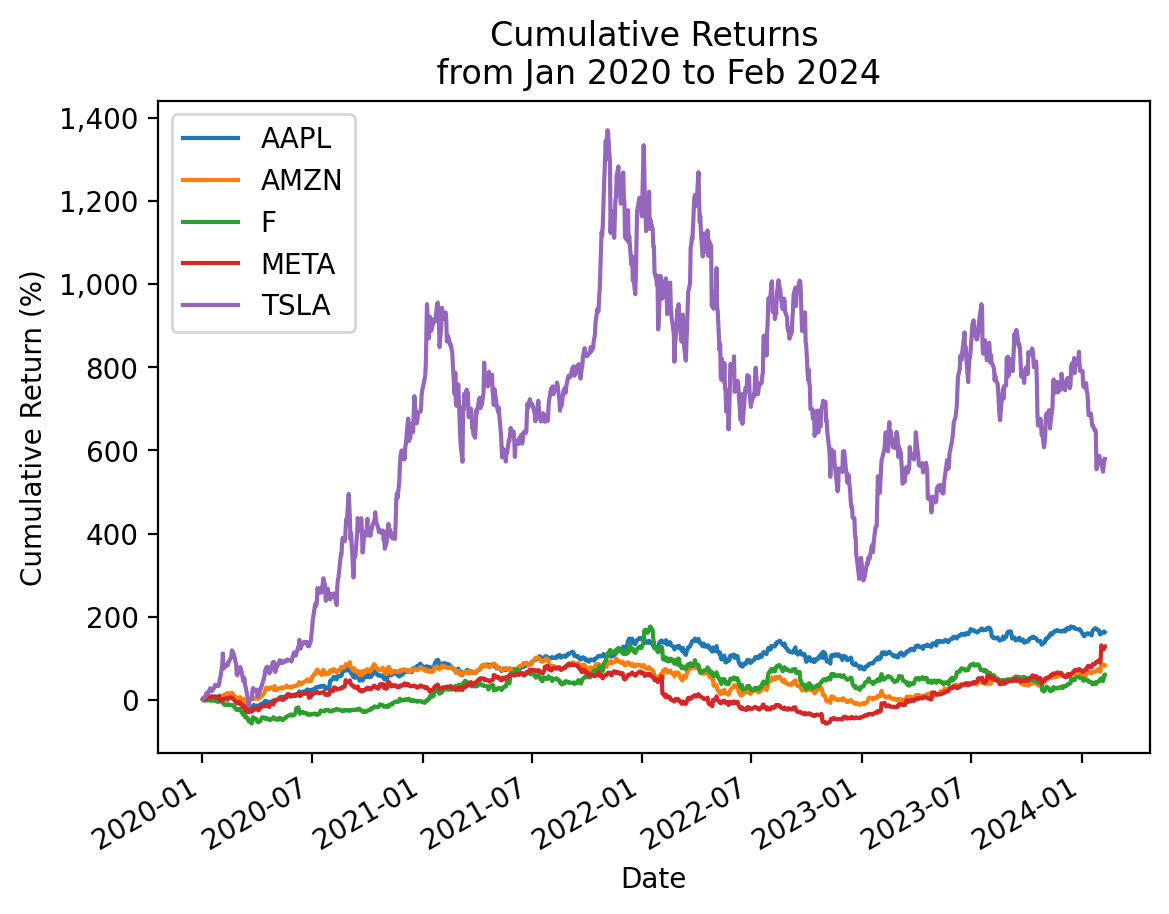
\includegraphics{herron_01_practice_03_files/figure-pdf/cell-13-output-1.png}

}

\end{figure}

\hypertarget{use-the-.cumsum-method-with-log-returns-to-plot-cumulative-returns-for-these-stocks-in-the-2020s-1}{%
\subsection{\texorpdfstring{Use the \texttt{.cumsum()} method with log
returns to plot cumulative returns for these stocks in the
2020s}{Use the .cumsum() method with log returns to plot cumulative returns for these stocks in the 2020s}}\label{use-the-.cumsum-method-with-log-returns-to-plot-cumulative-returns-for-these-stocks-in-the-2020s-1}}

\begin{Shaded}
\begin{Highlighting}[]
\NormalTok{cumret\_cumsum }\OperatorTok{=}\NormalTok{  (}
\NormalTok{    returns\_2020s }\CommentTok{\# start with simple returns}
\NormalTok{    .pipe(np.log1p) }\CommentTok{\# convert to log returns}
\NormalTok{    .cumsum() }\CommentTok{\# log returns are additive}
\NormalTok{    .pipe(np.expm1) }\CommentTok{\# convert back to simple returns}
\NormalTok{)}
\end{Highlighting}
\end{Shaded}

\begin{Shaded}
\begin{Highlighting}[]
\NormalTok{np.allclose(cumret\_cumsum, cumret\_cumprod)}
\end{Highlighting}
\end{Shaded}

\begin{verbatim}
True
\end{verbatim}

\begin{Shaded}
\begin{Highlighting}[]
\NormalTok{np.allclose(}\DecValTok{1}\OperatorTok{*}\DecValTok{10}\OperatorTok{**{-}}\DecValTok{9}\NormalTok{, }\FloatTok{1.1}\OperatorTok{*}\DecValTok{10}\OperatorTok{**{-}}\DecValTok{9}\NormalTok{)}
\end{Highlighting}
\end{Shaded}

\begin{verbatim}
True
\end{verbatim}

\begin{Shaded}
\begin{Highlighting}[]
\NormalTok{cumret\_cumsum.mul(}\DecValTok{100}\NormalTok{).plot()}

\CommentTok{\# https://stackoverflow.com/questions/25973581/how{-}to{-}format{-}axis{-}number{-}format{-}to{-}thousands{-}with{-}a{-}comma}
\ImportTok{from}\NormalTok{ matplotlib }\ImportTok{import}\NormalTok{ ticker}
\NormalTok{plt.gca().get\_yaxis().set\_major\_formatter(ticker.FuncFormatter(}\KeywordTok{lambda}\NormalTok{ x, p: }\BuiltInTok{format}\NormalTok{(}\BuiltInTok{int}\NormalTok{(x), }\StringTok{\textquotesingle{},\textquotesingle{}}\NormalTok{)))}

\NormalTok{plt.ylabel(}\StringTok{\textquotesingle{}Cumulative Return (\%)\textquotesingle{}}\NormalTok{)}
\NormalTok{plt.title(}\SpecialStringTok{f\textquotesingle{}Cumulative Returns}\CharTok{\textbackslash{}n}\SpecialStringTok{ from }\SpecialCharTok{\{}\NormalTok{returns\_2020s}\SpecialCharTok{.}\NormalTok{index}\SpecialCharTok{.}\BuiltInTok{min}\NormalTok{()}\SpecialCharTok{:}\OperatorTok{\%}\NormalTok{b }\OperatorTok{\%}\NormalTok{Y}\SpecialCharTok{\}}\SpecialStringTok{ to }\SpecialCharTok{\{}\NormalTok{returns\_2020s}\SpecialCharTok{.}\NormalTok{index}\SpecialCharTok{.}\BuiltInTok{max}\NormalTok{()}\SpecialCharTok{:}\OperatorTok{\%}\NormalTok{b }\OperatorTok{\%}\NormalTok{Y}\SpecialCharTok{\}}\SpecialStringTok{\textquotesingle{}}\NormalTok{)}
\NormalTok{plt.show()}
\end{Highlighting}
\end{Shaded}

\begin{figure}[H]

{\centering 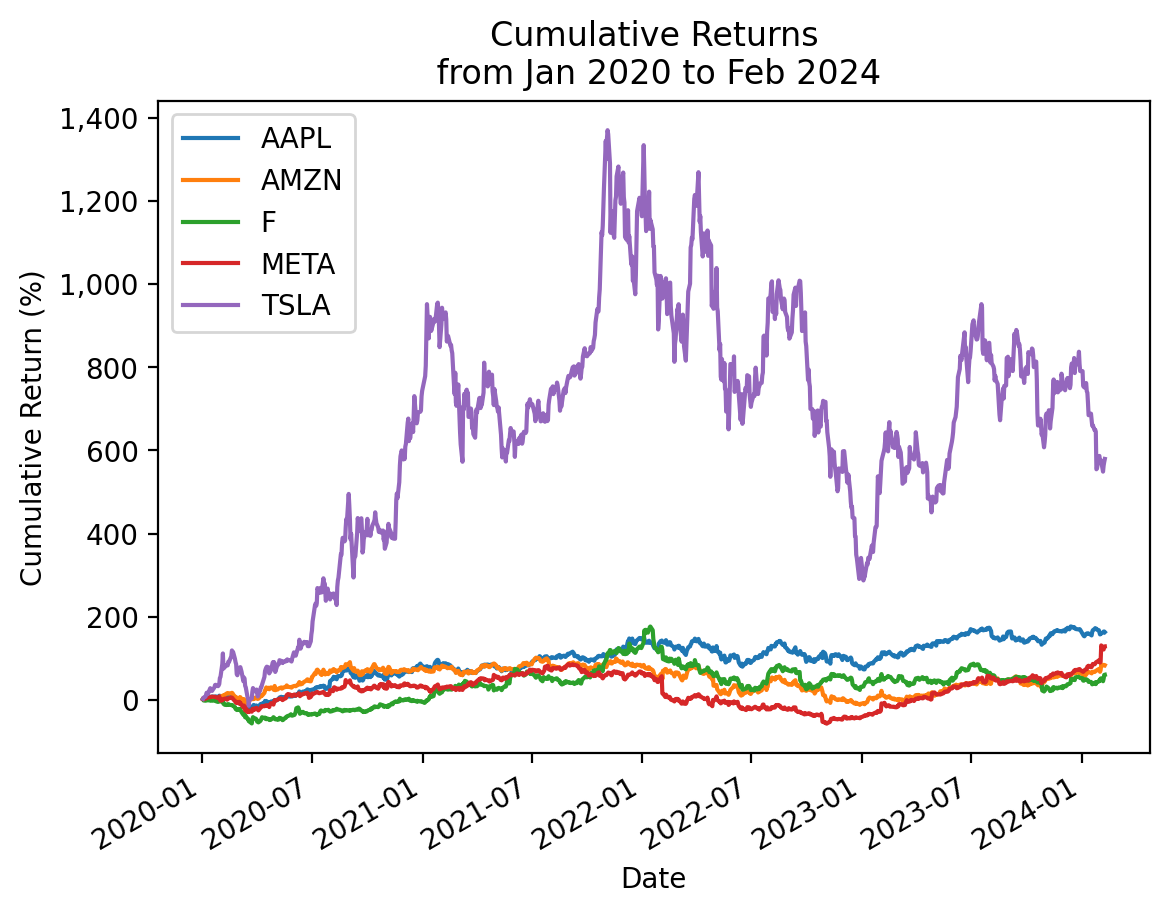
\includegraphics{herron_01_practice_03_files/figure-pdf/cell-17-output-1.png}

}

\end{figure}

\hypertarget{use-price-data-only-to-plot-cumulative-returns-for-these-stocks-in-the-2020s-1}{%
\subsection{Use price data only to plot cumulative returns for these
stocks in the
2020s}\label{use-price-data-only-to-plot-cumulative-returns-for-these-stocks-in-the-2020s-1}}

We can also calculate cumulative returns as the ratio of adjusted
closes. That is \(R_{0,T} = \frac{AC_T}{AC_0} - 1\). The trick here is
that \(FV_t = PV (1+r)^t\), so \((1+r)^t = \frac{FV_t}{PV}\).

\begin{Shaded}
\begin{Highlighting}[]
\NormalTok{returns\_2020s.iloc[}\DecValTok{0}\NormalTok{]}
\end{Highlighting}
\end{Shaded}

\begin{verbatim}
AAPL   0.0228
AMZN   0.0272
F      0.0129
META   0.0221
TSLA   0.0285
Name: 2020-01-02 00:00:00, dtype: float64
\end{verbatim}

\begin{Shaded}
\begin{Highlighting}[]
\NormalTok{cumret\_prices }\OperatorTok{=}\NormalTok{ prices[}\StringTok{\textquotesingle{}Adj Close\textquotesingle{}}\NormalTok{].loc[}\StringTok{\textquotesingle{}2020\textquotesingle{}}\NormalTok{:].iloc[:}\OperatorTok{{-}}\DecValTok{1}\NormalTok{] }\OperatorTok{/}\NormalTok{ prices[}\StringTok{\textquotesingle{}Adj Close\textquotesingle{}}\NormalTok{].loc[}\StringTok{\textquotesingle{}2019\textquotesingle{}}\NormalTok{].iloc[}\OperatorTok{{-}}\DecValTok{1}\NormalTok{] }\OperatorTok{{-}} \DecValTok{1}
\end{Highlighting}
\end{Shaded}

\begin{Shaded}
\begin{Highlighting}[]
\NormalTok{np.allclose(cumret\_prices, cumret\_cumprod)}
\end{Highlighting}
\end{Shaded}

\begin{verbatim}
True
\end{verbatim}

\begin{Shaded}
\begin{Highlighting}[]
\NormalTok{cumret\_prices.mul(}\DecValTok{100}\NormalTok{).plot()}

\CommentTok{\# https://stackoverflow.com/questions/25973581/how{-}to{-}format{-}axis{-}number{-}format{-}to{-}thousands{-}with{-}a{-}comma}
\ImportTok{from}\NormalTok{ matplotlib }\ImportTok{import}\NormalTok{ ticker}
\NormalTok{plt.gca().get\_yaxis().set\_major\_formatter(ticker.FuncFormatter(}\KeywordTok{lambda}\NormalTok{ x, p: }\BuiltInTok{format}\NormalTok{(}\BuiltInTok{int}\NormalTok{(x), }\StringTok{\textquotesingle{},\textquotesingle{}}\NormalTok{)))}

\NormalTok{plt.ylabel(}\StringTok{\textquotesingle{}Cumulative Return (\%)\textquotesingle{}}\NormalTok{)}
\NormalTok{plt.title(}\SpecialStringTok{f\textquotesingle{}Cumulative Returns}\CharTok{\textbackslash{}n}\SpecialStringTok{ from }\SpecialCharTok{\{}\NormalTok{returns\_2020s}\SpecialCharTok{.}\NormalTok{index}\SpecialCharTok{.}\BuiltInTok{min}\NormalTok{()}\SpecialCharTok{:}\OperatorTok{\%}\NormalTok{b }\OperatorTok{\%}\NormalTok{Y}\SpecialCharTok{\}}\SpecialStringTok{ to }\SpecialCharTok{\{}\NormalTok{returns\_2020s}\SpecialCharTok{.}\NormalTok{index}\SpecialCharTok{.}\BuiltInTok{max}\NormalTok{()}\SpecialCharTok{:}\OperatorTok{\%}\NormalTok{b }\OperatorTok{\%}\NormalTok{Y}\SpecialCharTok{\}}\SpecialStringTok{\textquotesingle{}}\NormalTok{)}
\NormalTok{plt.show()}
\end{Highlighting}
\end{Shaded}

\begin{figure}[H]

{\centering 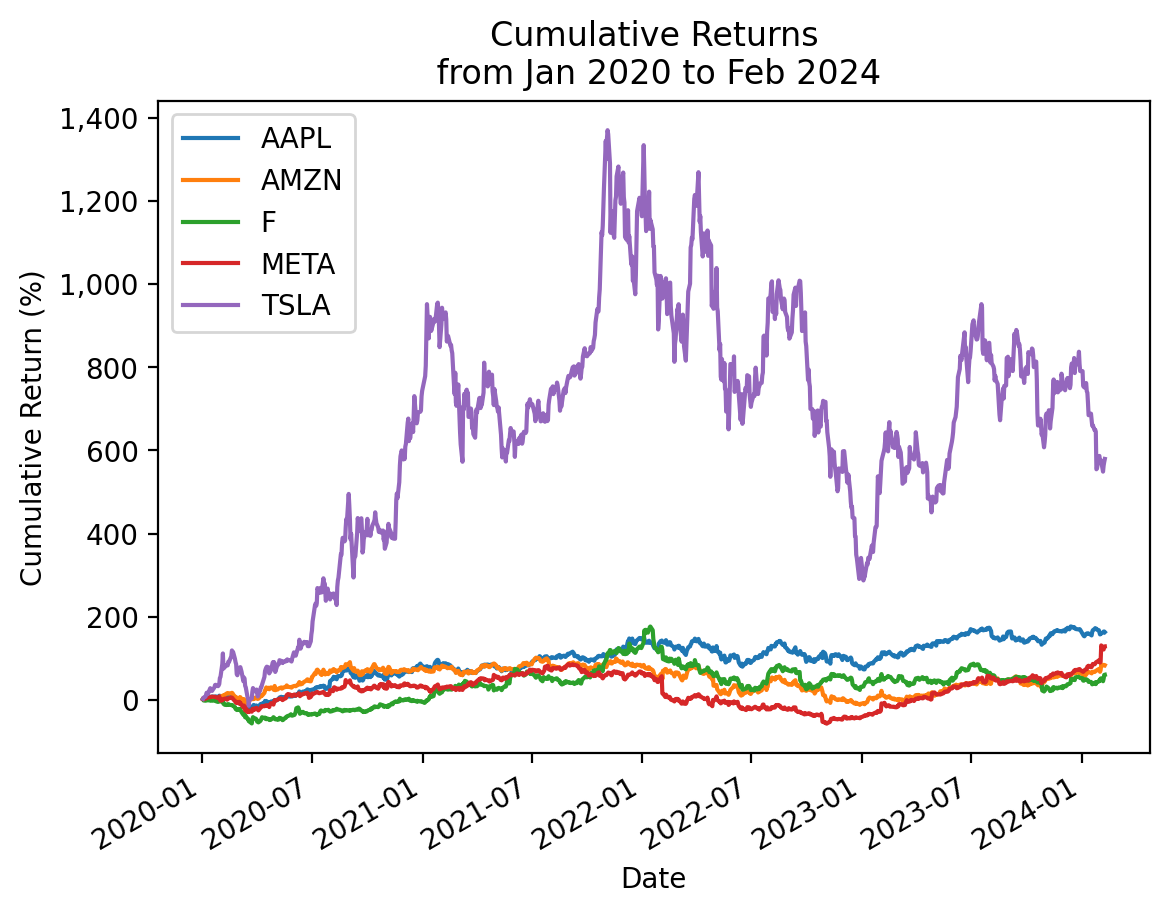
\includegraphics{herron_01_practice_03_files/figure-pdf/cell-21-output-1.png}

}

\end{figure}

\hypertarget{calculate-the-sharpe-ratio-for-tsla-1}{%
\subsection{Calculate the Sharpe Ratio for
TSLA}\label{calculate-the-sharpe-ratio-for-tsla-1}}

Calculate the Sharpe Ratio with all available returns and 2020s returns.
Recall the Sharpe Ratio is \(\frac{\overline{r_i - r_f}}{\sigma_i}\),
where \(\sigma_i\) is the volatility of \emph{excess} returns.

\textbf{\emph{I suggest you write a function named
\texttt{calc\_sharpe()} to use for the rest of this notebook.}}

\begin{Shaded}
\begin{Highlighting}[]
\KeywordTok{def}\NormalTok{ calc\_sharpe(ri, rf}\OperatorTok{=}\NormalTok{ff[}\StringTok{\textquotesingle{}RF\textquotesingle{}}\NormalTok{], ppy}\OperatorTok{=}\DecValTok{252}\NormalTok{):}
\NormalTok{    ri\_rf }\OperatorTok{=}\NormalTok{ ri.sub(rf).dropna()}
    \ControlFlowTok{return}\NormalTok{ np.sqrt(ppy) }\OperatorTok{*}\NormalTok{ ri\_rf.mean() }\OperatorTok{/}\NormalTok{ ri\_rf.std()}
\end{Highlighting}
\end{Shaded}

\begin{Shaded}
\begin{Highlighting}[]
\NormalTok{calc\_sharpe(ri}\OperatorTok{=}\NormalTok{returns[}\StringTok{\textquotesingle{}TSLA\textquotesingle{}}\NormalTok{])}
\end{Highlighting}
\end{Shaded}

\begin{verbatim}
0.9261
\end{verbatim}

\begin{Shaded}
\begin{Highlighting}[]
\NormalTok{calc\_sharpe(ri}\OperatorTok{=}\NormalTok{returns\_2020s[}\StringTok{\textquotesingle{}TSLA\textquotesingle{}}\NormalTok{])}
\end{Highlighting}
\end{Shaded}

\begin{verbatim}
1.1212
\end{verbatim}

\textbf{\emph{Or, we can use the \texttt{.pipe()} method because
\texttt{ri} is the first argument to \texttt{calc\_sharpe()}!}}

\begin{Shaded}
\begin{Highlighting}[]
\NormalTok{returns[}\StringTok{\textquotesingle{}TSLA\textquotesingle{}}\NormalTok{].pipe(calc\_sharpe)}
\end{Highlighting}
\end{Shaded}

\begin{verbatim}
0.9261
\end{verbatim}

\begin{Shaded}
\begin{Highlighting}[]
\NormalTok{returns\_2020s[}\StringTok{\textquotesingle{}TSLA\textquotesingle{}}\NormalTok{].pipe(calc\_sharpe)}
\end{Highlighting}
\end{Shaded}

\begin{verbatim}
1.1212
\end{verbatim}

\hypertarget{calculate-the-market-beta-for-tsla-1}{%
\subsection{Calculate the market beta for
TSLA}\label{calculate-the-market-beta-for-tsla-1}}

Calculate the market beta with all available returns and 2020s returns.
Recall we estimate market beta with the ordinary least squares (OLS)
regression \(R_i-R_f = \alpha + \beta (R_m-R_f) + \epsilon\). We can
estimate market beta with the covariance formula (i.e.,
\(\beta_i = \frac{Cov(R_i - R_f, R_m - R_f)}{Var(R_m-R_f)}\)) above for
a univariate regression if we do not need goodness of fit statistics.

\textbf{\emph{I suggest you write a function named \texttt{calc\_beta()}
to use for the rest of this notebook.}}

\begin{Shaded}
\begin{Highlighting}[]
\KeywordTok{def}\NormalTok{ calc\_beta(ri, rf}\OperatorTok{=}\NormalTok{ff[}\StringTok{\textquotesingle{}RF\textquotesingle{}}\NormalTok{], rm\_rf}\OperatorTok{=}\NormalTok{ff[}\StringTok{\textquotesingle{}Mkt{-}RF\textquotesingle{}}\NormalTok{]):}
\NormalTok{    ri\_rf }\OperatorTok{=}\NormalTok{ ri.sub(rf).dropna()}
    \ControlFlowTok{return}\NormalTok{ ri\_rf.cov(rm\_rf) }\OperatorTok{/}\NormalTok{ rm\_rf.loc[ri\_rf.index].var()}
\end{Highlighting}
\end{Shaded}

\begin{Shaded}
\begin{Highlighting}[]
\NormalTok{calc\_beta(ri}\OperatorTok{=}\NormalTok{returns[}\StringTok{\textquotesingle{}TSLA\textquotesingle{}}\NormalTok{])}
\end{Highlighting}
\end{Shaded}

\begin{verbatim}
1.4417
\end{verbatim}

\begin{Shaded}
\begin{Highlighting}[]
\NormalTok{calc\_beta(ri}\OperatorTok{=}\NormalTok{returns\_2020s[}\StringTok{\textquotesingle{}TSLA\textquotesingle{}}\NormalTok{])}
\end{Highlighting}
\end{Shaded}

\begin{verbatim}
1.5780
\end{verbatim}

\textbf{\emph{Or, we can use the \texttt{.pipe()} method because
\texttt{ri} is the first argument to \texttt{calc\_sharpe()}!}}

\begin{Shaded}
\begin{Highlighting}[]
\NormalTok{returns[}\StringTok{\textquotesingle{}TSLA\textquotesingle{}}\NormalTok{].pipe(calc\_beta)}
\end{Highlighting}
\end{Shaded}

\begin{verbatim}
1.4417
\end{verbatim}

\begin{Shaded}
\begin{Highlighting}[]
\NormalTok{returns\_2020s[}\StringTok{\textquotesingle{}TSLA\textquotesingle{}}\NormalTok{].pipe(calc\_beta)}
\end{Highlighting}
\end{Shaded}

\begin{verbatim}
1.5780
\end{verbatim}

\hypertarget{guess-the-sharpe-ratios-for-these-stocks-in-the-2020s-1}{%
\subsection{Guess the Sharpe Ratios for these stocks in the
2020s}\label{guess-the-sharpe-ratios-for-these-stocks-in-the-2020s-1}}

\hypertarget{guess-the-market-betas-for-these-stocks-in-the-2020s-1}{%
\subsection{Guess the market betas for these stocks in the
2020s}\label{guess-the-market-betas-for-these-stocks-in-the-2020s-1}}

\hypertarget{calculate-the-sharpe-ratios-for-these-stocks-in-the-2020s-1}{%
\subsection{Calculate the Sharpe Ratios for these stocks in the
2020s}\label{calculate-the-sharpe-ratios-for-these-stocks-in-the-2020s-1}}

How good were your guesses?

\begin{Shaded}
\begin{Highlighting}[]
\ControlFlowTok{for}\NormalTok{ i }\KeywordTok{in}\NormalTok{ returns\_2020s:}
\NormalTok{    sharpe\_i }\OperatorTok{=}\NormalTok{ returns\_2020s[i].pipe(calc\_sharpe)}
    \BuiltInTok{print}\NormalTok{(}\SpecialStringTok{f\textquotesingle{}Sharpe Ratio for }\SpecialCharTok{\{}\NormalTok{i}\SpecialCharTok{\}}\SpecialStringTok{:}\CharTok{\textbackslash{}t}\SpecialStringTok{ }\SpecialCharTok{\{}\NormalTok{sharpe\_i}\SpecialCharTok{:0.2f\}}\SpecialStringTok{\textquotesingle{}}\NormalTok{)}
\end{Highlighting}
\end{Shaded}

\begin{verbatim}
Sharpe Ratio for AAPL:   0.86
Sharpe Ratio for AMZN:   0.48
Sharpe Ratio for F:  0.42
Sharpe Ratio for META:   0.49
Sharpe Ratio for TSLA:   1.12
\end{verbatim}

We can also use pandas notation to vectorize this calculation. First
calculate \emph{excess} returns as \(r_i - r_f\).

\begin{Shaded}
\begin{Highlighting}[]
\NormalTok{returns\_2020s\_excess }\OperatorTok{=}\NormalTok{ returns\_2020s.sub(ff[}\StringTok{\textquotesingle{}RF\textquotesingle{}}\NormalTok{], axis}\OperatorTok{=}\DecValTok{0}\NormalTok{).dropna()}
\end{Highlighting}
\end{Shaded}

Then use pandas notation to calculate means, standard deviations, and
annualize.

\begin{Shaded}
\begin{Highlighting}[]
\NormalTok{(}
\NormalTok{    returns\_2020s\_excess}
\NormalTok{    .mean()}
\NormalTok{    .div(returns\_2020s\_excess.std())}
\NormalTok{    .mul(np.sqrt(}\DecValTok{252}\NormalTok{))}
\NormalTok{)}
\end{Highlighting}
\end{Shaded}

\begin{verbatim}
AAPL   0.8576
AMZN   0.4750
F      0.4240
META   0.4949
TSLA   1.1212
dtype: float64
\end{verbatim}

\textbf{\emph{Note:}} In a few weeks we will learn the \texttt{.apply()}
method, which avoids the loop syntax.

\begin{Shaded}
\begin{Highlighting}[]
\NormalTok{returns\_2020s.}\BuiltInTok{apply}\NormalTok{(calc\_sharpe)}
\end{Highlighting}
\end{Shaded}

\begin{verbatim}
AAPL   0.8576
AMZN   0.4750
F      0.4240
META   0.4949
TSLA   1.1212
dtype: float64
\end{verbatim}

\hypertarget{calculate-the-market-betas-for-these-stocks-in-the-2020s-1}{%
\subsection{Calculate the market betas for these stocks in the
2020s}\label{calculate-the-market-betas-for-these-stocks-in-the-2020s-1}}

How good were your guesses?

\begin{Shaded}
\begin{Highlighting}[]
\ControlFlowTok{for}\NormalTok{ i }\KeywordTok{in}\NormalTok{ returns\_2020s:}
\NormalTok{    beta\_i }\OperatorTok{=}\NormalTok{ returns\_2020s[i].pipe(calc\_beta)}
    \BuiltInTok{print}\NormalTok{(}\SpecialStringTok{f\textquotesingle{}Beta for }\SpecialCharTok{\{}\NormalTok{i}\SpecialCharTok{\}}\SpecialStringTok{:}\CharTok{\textbackslash{}t}\SpecialStringTok{ }\SpecialCharTok{\{}\NormalTok{beta\_i}\SpecialCharTok{:0.2f\}}\SpecialStringTok{\textquotesingle{}}\NormalTok{)}
\end{Highlighting}
\end{Shaded}

\begin{verbatim}
Beta for AAPL:   1.15
Beta for AMZN:   1.04
Beta for F:  1.22
Beta for META:   1.27
Beta for TSLA:   1.58
\end{verbatim}

Or we can follow out approach above to vectorize this calculation.
First, we need to add a market excess return column to
\texttt{returns\_2020s\_excess}.

\begin{Shaded}
\begin{Highlighting}[]
\NormalTok{returns\_2020s\_excess[}\StringTok{\textquotesingle{}Mkt{-}RF\textquotesingle{}}\NormalTok{] }\OperatorTok{=}\NormalTok{ ff[}\StringTok{\textquotesingle{}Mkt{-}RF\textquotesingle{}}\NormalTok{]}
\NormalTok{returns\_2020s\_excess.head()}
\end{Highlighting}
\end{Shaded}

\begin{longtable}[]{@{}lllllll@{}}
\toprule\noalign{}
& AAPL & AMZN & F & META & TSLA & Mkt-RF \\
Date & & & & & & \\
\midrule\noalign{}
\endhead
\bottomrule\noalign{}
\endlastfoot
2020-01-02 & 0.0228 & 0.0271 & 0.0128 & 0.0220 & 0.0285 & 0.0086 \\
2020-01-03 & -0.0098 & -0.0122 & -0.0224 & -0.0054 & 0.0296 & -0.0067 \\
2020-01-06 & 0.0079 & 0.0148 & -0.0055 & 0.0188 & 0.0192 & 0.0036 \\
2020-01-07 & -0.0048 & 0.0020 & 0.0098 & 0.0021 & 0.0387 & -0.0019 \\
2020-01-08 & 0.0160 & -0.0079 & -0.0001 & 0.0101 & 0.0491 & 0.0047 \\
\end{longtable}

\begin{Shaded}
\begin{Highlighting}[]
\NormalTok{vcv }\OperatorTok{=}\NormalTok{ returns\_2020s\_excess.cov()}
\NormalTok{vcv}
\end{Highlighting}
\end{Shaded}

\begin{longtable}[]{@{}lllllll@{}}
\toprule\noalign{}
& AAPL & AMZN & F & META & TSLA & Mkt-RF \\
\midrule\noalign{}
\endhead
\bottomrule\noalign{}
\endlastfoot
AAPL & 0.0004 & 0.0003 & 0.0002 & 0.0004 & 0.0005 & 0.0003 \\
AMZN & 0.0003 & 0.0006 & 0.0002 & 0.0004 & 0.0005 & 0.0002 \\
F & 0.0002 & 0.0002 & 0.0009 & 0.0003 & 0.0005 & 0.0003 \\
META & 0.0004 & 0.0004 & 0.0003 & 0.0009 & 0.0005 & 0.0003 \\
TSLA & 0.0005 & 0.0005 & 0.0005 & 0.0005 & 0.0018 & 0.0003 \\
Mkt-RF & 0.0003 & 0.0002 & 0.0003 & 0.0003 & 0.0003 & 0.0002 \\
\end{longtable}

\begin{Shaded}
\begin{Highlighting}[]
\NormalTok{vcv[}\StringTok{\textquotesingle{}Mkt{-}RF\textquotesingle{}}\NormalTok{].div(vcv.loc[}\StringTok{\textquotesingle{}Mkt{-}RF\textquotesingle{}}\NormalTok{, }\StringTok{\textquotesingle{}Mkt{-}RF\textquotesingle{}}\NormalTok{]).plot(kind}\OperatorTok{=}\StringTok{\textquotesingle{}bar\textquotesingle{}}\NormalTok{)}
\NormalTok{plt.xlabel(}\StringTok{\textquotesingle{}Ticker\textquotesingle{}}\NormalTok{)}
\NormalTok{plt.ylabel(}\StringTok{\textquotesingle{}CAPM Beta\textquotesingle{}}\NormalTok{)}
\NormalTok{plt.title(}\StringTok{\textquotesingle{}CAPM Betas\textquotesingle{}}\NormalTok{)}
\NormalTok{plt.show()}
\end{Highlighting}
\end{Shaded}

\begin{figure}[H]

{\centering \includegraphics{herron_01_practice_03_files/figure-pdf/cell-39-output-1.png}

}

\end{figure}

\textbf{\emph{Note:}} In a few weeks we will learn the \texttt{.apply()}
method, which avoids the loop syntax.

\begin{Shaded}
\begin{Highlighting}[]
\NormalTok{returns\_2020s.}\BuiltInTok{apply}\NormalTok{(calc\_beta)}
\end{Highlighting}
\end{Shaded}

\begin{verbatim}
AAPL   1.1541
AMZN   1.0429
F      1.2231
META   1.2710
TSLA   1.5780
dtype: float64
\end{verbatim}

\hypertarget{calculate-the-sharpe-ratio-for-an-equally-weighted-portfolio-of-these-stocks-in-the-2020s-1}{%
\subsection{\texorpdfstring{Calculate the Sharpe Ratio for an
\emph{equally weighted} portfolio of these stocks in the
2020s}{Calculate the Sharpe Ratio for an equally weighted portfolio of these stocks in the 2020s}}\label{calculate-the-sharpe-ratio-for-an-equally-weighted-portfolio-of-these-stocks-in-the-2020s-1}}

What do you notice?

\begin{Shaded}
\begin{Highlighting}[]
\NormalTok{returns\_2020s.mean(axis}\OperatorTok{=}\DecValTok{1}\NormalTok{).pipe(calc\_sharpe)}
\end{Highlighting}
\end{Shaded}

\begin{verbatim}
0.9573
\end{verbatim}

Because diversification reduces portfolio standard deviation less than
the sum of its parts, the Sharpe Ratio of the equally weighted portfolio
is less than the equally weighted mean of the single-stock Sharpe
Ratios.

\begin{Shaded}
\begin{Highlighting}[]
\NormalTok{returns\_2020s.}\BuiltInTok{apply}\NormalTok{(calc\_sharpe).mean()}
\end{Highlighting}
\end{Shaded}

\begin{verbatim}
0.6745
\end{verbatim}

\hypertarget{calculate-the-market-beta-for-an-equally-weighted-portfolio-of-these-stocks-in-the-2020s-1}{%
\subsection{\texorpdfstring{Calculate the market beta for an
\emph{equally weighted} portfolio of these stocks in the
2020s}{Calculate the market beta for an equally weighted portfolio of these stocks in the 2020s}}\label{calculate-the-market-beta-for-an-equally-weighted-portfolio-of-these-stocks-in-the-2020s-1}}

What do you notice?

Beta measures \emph{non}diversifiable risk, so
\(\beta_P = \sum w_i \beta_i\)!

\begin{Shaded}
\begin{Highlighting}[]
\NormalTok{returns\_2020s.mean(axis}\OperatorTok{=}\DecValTok{1}\NormalTok{).pipe(calc\_beta)}
\end{Highlighting}
\end{Shaded}

\begin{verbatim}
1.2538
\end{verbatim}

\begin{Shaded}
\begin{Highlighting}[]
\NormalTok{returns\_2020s.}\BuiltInTok{apply}\NormalTok{(calc\_beta).mean()}
\end{Highlighting}
\end{Shaded}

\begin{verbatim}
1.2538
\end{verbatim}

\hypertarget{calculate-the-market-betas-for-these-stocks-every-calendar-year-for-every-possible-year-1}{%
\subsection{Calculate the market betas for these stocks every calendar
year for every possible
year}\label{calculate-the-market-betas-for-these-stocks-every-calendar-year-for-every-possible-year-1}}

Save these market betas to data frame \texttt{betas}. Our current Python
knowledge limits us to a for-loop, but we will learn easier and faster
approaches soon!

\begin{Shaded}
\begin{Highlighting}[]
\NormalTok{betas }\OperatorTok{=}\NormalTok{ pd.DataFrame(}
\NormalTok{    index}\OperatorTok{=}\BuiltInTok{range}\NormalTok{(}\DecValTok{1972}\NormalTok{, }\DecValTok{2024}\NormalTok{),}
\NormalTok{    columns}\OperatorTok{=}\NormalTok{returns.columns}
\NormalTok{)}

\NormalTok{betas.columns.name }\OperatorTok{=} \StringTok{\textquotesingle{}Ticker\textquotesingle{}}
\NormalTok{betas.index.name }\OperatorTok{=} \StringTok{\textquotesingle{}Year\textquotesingle{}}

\NormalTok{betas.tail()}
\end{Highlighting}
\end{Shaded}

\begin{longtable}[]{@{}llllll@{}}
\toprule\noalign{}
Ticker & AAPL & AMZN & F & META & TSLA \\
Year & & & & & \\
\midrule\noalign{}
\endhead
\bottomrule\noalign{}
\endlastfoot
2019 & NaN & NaN & NaN & NaN & NaN \\
2020 & NaN & NaN & NaN & NaN & NaN \\
2021 & NaN & NaN & NaN & NaN & NaN \\
2022 & NaN & NaN & NaN & NaN & NaN \\
2023 & NaN & NaN & NaN & NaN & NaN \\
\end{longtable}

\begin{Shaded}
\begin{Highlighting}[]
\ControlFlowTok{for}\NormalTok{ i }\KeywordTok{in}\NormalTok{ betas.index: }
    \ControlFlowTok{for}\NormalTok{ c }\KeywordTok{in}\NormalTok{ betas.columns:}
\NormalTok{        betas.at[i, c] }\OperatorTok{=}\NormalTok{ returns.loc[}\BuiltInTok{str}\NormalTok{(i), c].pipe(calc\_beta)}

\NormalTok{betas.tail()}
\end{Highlighting}
\end{Shaded}

\begin{longtable}[]{@{}llllll@{}}
\toprule\noalign{}
Ticker & AAPL & AMZN & F & META & TSLA \\
Year & & & & & \\
\midrule\noalign{}
\endhead
\bottomrule\noalign{}
\endlastfoot
2019 & 1.4751 & 1.2752 & 1.0733 & 1.2094 & 1.3262 \\
2020 & 1.1174 & 0.6866 & 1.1052 & 0.9913 & 1.3041 \\
2021 & 1.1957 & 0.9822 & 1.2396 & 1.2014 & 1.9891 \\
2022 & 1.2386 & 1.5922 & 1.3824 & 1.6843 & 1.7414 \\
2023 & 1.0369 & 1.4649 & 1.3947 & 1.6630 & 2.2218 \\
\end{longtable}

\hypertarget{plot-the-time-series-of-market-betas-1}{%
\subsection{Plot the time series of market
betas}\label{plot-the-time-series-of-market-betas-1}}

\begin{Shaded}
\begin{Highlighting}[]
\NormalTok{betas.plot()}
\NormalTok{plt.ylabel(}\StringTok{\textquotesingle{}CAPM Beta\textquotesingle{}}\NormalTok{)}
\NormalTok{plt.title(}\StringTok{\textquotesingle{}CAPM Betas\textquotesingle{}}\NormalTok{)}
\NormalTok{plt.show()}
\end{Highlighting}
\end{Shaded}

\begin{figure}[H]

{\centering 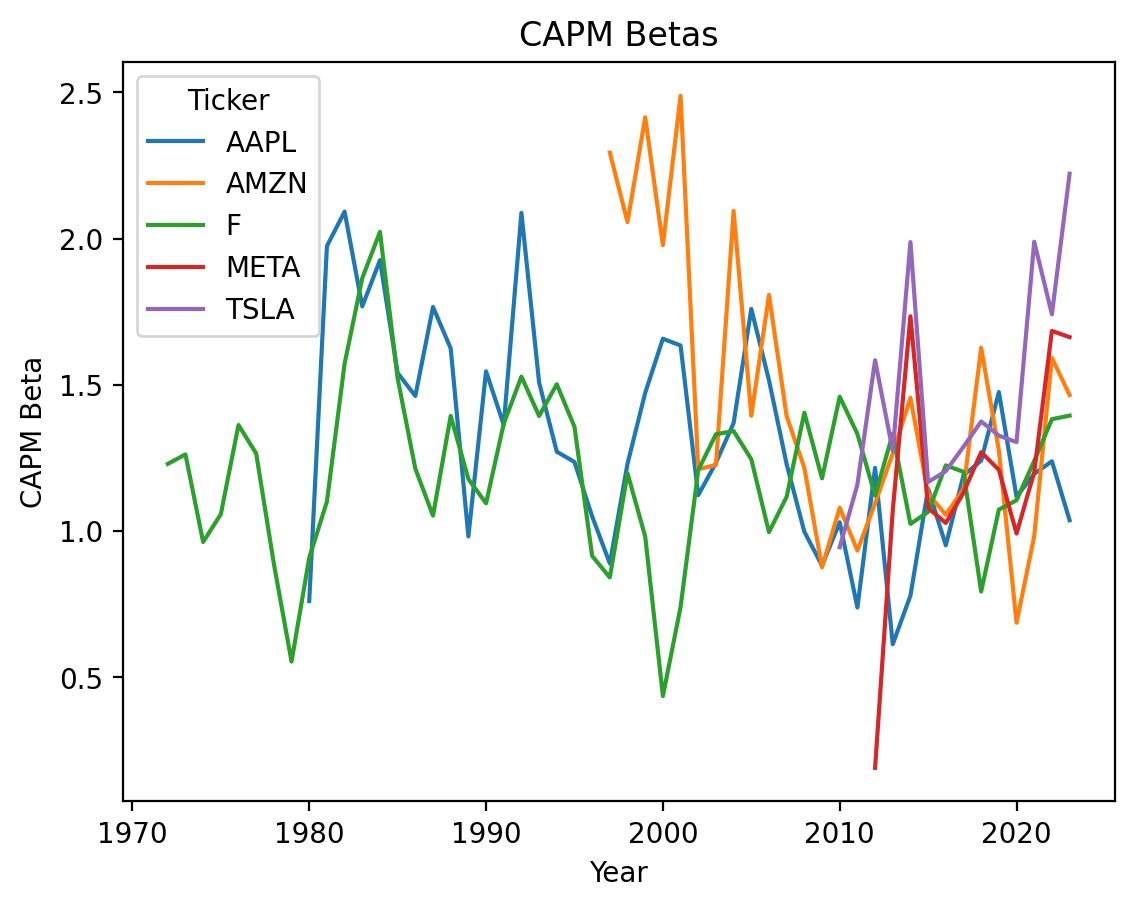
\includegraphics{herron_01_practice_03_files/figure-pdf/cell-47-output-1.png}

}

\end{figure}

\hypertarget{herron-topic-1---practice-for-section-04}{%
\chapter{Herron Topic 1 - Practice for Section
04}\label{herron-topic-1---practice-for-section-04}}

\hypertarget{announcements-18}{%
\section{Announcements}\label{announcements-18}}

\begin{enumerate}
\def\labelenumi{\arabic{enumi}.}
\tightlist
\item
  DataCamp

  \begin{enumerate}
  \def\labelenumii{\arabic{enumii}.}
  \tightlist
  \item
    \emph{Data Manipulation with pandas} due by Friday, 2/9, at 11:59 PM
  \item
    \emph{Joining Data with pandas} due by Friday, 2/16, at 11:59 PM
  \item
    \emph{Earn 10,000 XP} due by Friday, 3/15, at 11:59 PM
  \end{enumerate}
\item
  I posted Project 1 to Canvas

  \begin{enumerate}
  \def\labelenumii{\arabic{enumii}.}
  \tightlist
  \item
    Slides and notebook due by Friday, 2/23, at 11:59 PM
  \item
    Keep joining teams and let me know if you need help
  \end{enumerate}
\end{enumerate}

\hypertarget{minute-recap-17}{%
\section{10-Minute Recap}\label{minute-recap-17}}

\begin{Shaded}
\begin{Highlighting}[]
\ImportTok{import}\NormalTok{ matplotlib.pyplot }\ImportTok{as}\NormalTok{ plt}
\ImportTok{import}\NormalTok{ numpy }\ImportTok{as}\NormalTok{ np}
\ImportTok{import}\NormalTok{ pandas }\ImportTok{as}\NormalTok{ pd}
\ImportTok{import}\NormalTok{ pandas\_datareader }\ImportTok{as}\NormalTok{ pdr}
\ImportTok{import}\NormalTok{ yfinance }\ImportTok{as}\NormalTok{ yf}
\end{Highlighting}
\end{Shaded}

\begin{Shaded}
\begin{Highlighting}[]
\OperatorTok{\%}\NormalTok{precision }\DecValTok{4}
\NormalTok{pd.options.display.float\_format }\OperatorTok{=} \StringTok{\textquotesingle{}}\SpecialCharTok{\{:.4f\}}\StringTok{\textquotesingle{}}\NormalTok{.}\BuiltInTok{format}
\OperatorTok{\%}\NormalTok{config InlineBackend.figure\_format }\OperatorTok{=} \StringTok{\textquotesingle{}retina\textquotesingle{}}
\end{Highlighting}
\end{Shaded}

\begin{Shaded}
\begin{Highlighting}[]
\NormalTok{np.expm1(np.log1p(}\FloatTok{0.1}\NormalTok{))}
\end{Highlighting}
\end{Shaded}

\begin{verbatim}
0.1000
\end{verbatim}

First, we will use two packages to download data from the web:

\begin{enumerate}
\def\labelenumi{\arabic{enumi}.}
\tightlist
\item
  \texttt{yfinance} for Yahoo! Finance data
\item
  \texttt{pandas-datareader} for Ken French data (or FRED data to
  others)
\end{enumerate}

Second, there are ``simple returns'' and ``log returns''

\begin{enumerate}
\def\labelenumi{\arabic{enumi}.}
\tightlist
\item
  Simple returns are the returns that investors receive that we learned
  in FINA 6331 and FINA 6333:
  \(r_t = \frac{p_t + d_t - p_{t-1}}{p_{t-1}}\)
\item
  Log returns are the log of one plus simple returns. Why do we use
  them?

  \begin{enumerate}
  \def\labelenumii{\arabic{enumii}.}
  \tightlist
  \item
    \textbf{\emph{Log returns are additive}}, while simple returns are
    multiplicative. This additive property makes math really easy with
    log returns:
    \(\log(\prod_{t=0}^T (1 + r_t)) = \sum_{t=0}^T \log(1+r_t)\), so
    \(r_{0,T} = \prod_{t=0}^T (1 + r_t) - 1 = e^{\sum_{t=0}^T \log(1+r_t)} - 1\)
  \item
    \textbf{\emph{Log returns are almost normally distributed}}
  \end{enumerate}
\end{enumerate}

\textbf{\emph{We will almost always use simple returns.}} The exeception
is time-consuming calculations, which we will often do in log returns to
save us time.

Third, we can calculate portfolio returns easily in pandas!

\begin{enumerate}
\def\labelenumi{\arabic{enumi}.}
\tightlist
\item
  \texttt{returns.mean(axis=1)} is the return on an equally-weighted
  portfolio, \textbf{\emph{rebalanced at the same frequency as the
  returns in \texttt{returns}!}}
\item
  \texttt{returns.dot(weights)} is the return on a portfolio weighted
  according to the weights in the \texttt{weights} array,
  \textbf{\emph{still rebalanced at the same frequency as the returns in
  \texttt{returns}!}}
\end{enumerate}

\hypertarget{practice-18}{%
\section{Practice}\label{practice-18}}

\hypertarget{download-all-available-daily-price-data-for-tickers-tsla-f-aapl-amzn-and-meta-to-data-frame-prices-2}{%
\subsection{\texorpdfstring{Download all available daily price data for
tickers TSLA, F, AAPL, AMZN, and META to data frame
\texttt{prices}}{Download all available daily price data for tickers TSLA, F, AAPL, AMZN, and META to data frame prices}}\label{download-all-available-daily-price-data-for-tickers-tsla-f-aapl-amzn-and-meta-to-data-frame-prices-2}}

\begin{Shaded}
\begin{Highlighting}[]
\NormalTok{tickers }\OperatorTok{=} \StringTok{\textquotesingle{}TSLA F AAPL AMZN META\textquotesingle{}}
\NormalTok{prices }\OperatorTok{=}\NormalTok{ yf.download(tickers}\OperatorTok{=}\NormalTok{tickers)}

\NormalTok{prices}
\end{Highlighting}
\end{Shaded}

\begin{verbatim}
[*********************100%%**********************]  5 of 5 completed
\end{verbatim}

\begin{longtable}[]{@{}llllllllllllllllllllll@{}}
\toprule\noalign{}
&
\multicolumn{5}{>{\raggedright\arraybackslash}p{(\columnwidth - 42\tabcolsep) * \real{0.0000} + 8\tabcolsep}}{%
Adj Close} &
\multicolumn{5}{>{\raggedright\arraybackslash}p{(\columnwidth - 42\tabcolsep) * \real{0.0000} + 8\tabcolsep}}{%
Close} & ... &
\multicolumn{5}{>{\raggedright\arraybackslash}p{(\columnwidth - 42\tabcolsep) * \real{0.0000} + 8\tabcolsep}}{%
Open} &
\multicolumn{5}{>{\raggedright\arraybackslash}p{(\columnwidth - 42\tabcolsep) * \real{0.0000} + 8\tabcolsep}@{}}{%
Volume} \\
& AAPL & AMZN & F & META & TSLA & AAPL & AMZN & F & META & TSLA & ... &
AAPL & AMZN & F & META & TSLA & AAPL & AMZN & F & META & TSLA \\
Date & & & & & & & & & & & & & & & & & & & & & \\
\midrule\noalign{}
\endhead
\bottomrule\noalign{}
\endlastfoot
1972-06-01 & NaN & NaN & 0.2419 & NaN & NaN & NaN & NaN & 2.1532 & NaN &
NaN & ... & NaN & NaN & 0.0000 & NaN & NaN & NaN & NaN & 1091238 & NaN &
NaN \\
1972-06-02 & NaN & NaN & 0.2414 & NaN & NaN & NaN & NaN & 2.1492 & NaN &
NaN & ... & NaN & NaN & 2.1532 & NaN & NaN & NaN & NaN & 1174468 & NaN &
NaN \\
1972-06-05 & NaN & NaN & 0.2414 & NaN & NaN & NaN & NaN & 2.1492 & NaN &
NaN & ... & NaN & NaN & 2.1492 & NaN & NaN & NaN & NaN & 5209582 & NaN &
NaN \\
1972-06-06 & NaN & NaN & 0.2387 & NaN & NaN & NaN & NaN & 2.1248 & NaN &
NaN & ... & NaN & NaN & 2.1492 & NaN & NaN & NaN & NaN & 1424158 & NaN &
NaN \\
1972-06-07 & NaN & NaN & 0.2373 & NaN & NaN & NaN & NaN & 2.1127 & NaN &
NaN & ... & NaN & NaN & 2.1248 & NaN & NaN & NaN & NaN & 675088 & NaN &
NaN \\
... & ... & ... & ... & ... & ... & ... & ... & ... & ... & ... & ... &
... & ... & ... & ... & ... & ... & ... & ... & ... & ... \\
2024-02-05 & 187.6800 & 170.3100 & 11.5900 & 459.4100 & 181.0600 &
187.6800 & 170.3100 & 11.5900 & 459.4100 & 181.0600 & ... & 188.1500 &
170.2000 & 12.0100 & 469.8800 & 184.2600 & 69668800.0000 & 55081300.0000
& 81026800 & 40832400.0000 & 134294400.0000 \\
2024-02-06 & 189.3000 & 169.1500 & 12.0700 & 454.7200 & 185.1000 &
189.3000 & 169.1500 & 12.0700 & 454.7200 & 185.1000 & ... & 186.8600 &
169.3900 & 11.6400 & 464.0000 & 177.2100 & 43490800.0000 & 42505500.0000
& 98636800 & 21655200.0000 & 122676000.0000 \\
2024-02-07 & 189.4100 & 170.5300 & 12.8000 & 469.5900 & 187.5800 &
189.4100 & 170.5300 & 12.8000 & 469.5900 & 187.5800 & ... & 190.6400 &
169.4800 & 12.7300 & 458.0000 & 188.1800 & 53439000.0000 & 47174100.0000
& 137224000 & 23066000.0000 & 111535200.0000 \\
2024-02-08 & 188.3200 & 169.8400 & 12.8300 & 470.0000 & 189.5600 &
188.3200 & 169.8400 & 12.8300 & 470.0000 & 189.5600 & ... & 189.3900 &
169.6500 & 12.8700 & 468.3200 & 189.0000 & 40962000.0000 & 42316500.0000
& 68653900 & 18815100.0000 & 83034000.0000 \\
2024-02-09 & 188.8500 & 174.4500 & 12.6800 & 468.1100 & 193.5700 &
188.8500 & 174.4500 & 12.6800 & 468.1100 & 193.5700 & ... & 188.6500 &
170.9000 & 12.8100 & 472.9500 & 190.1800 & 43728065.0000 & 56886544.0000
& 46925766 & 18159624.0000 & 84009121.0000 \\
\end{longtable}

\hypertarget{calculate-all-available-daily-returns-and-save-to-data-frame-returns-2}{%
\subsection{\texorpdfstring{Calculate all available daily returns and
save to data frame
\texttt{returns}}{Calculate all available daily returns and save to data frame returns}}\label{calculate-all-available-daily-returns-and-save-to-data-frame-returns-2}}

\hypertarget{calculate-all-available-daily-returns-and-save-to-data-frame-returns-3}{%
\subsection{\texorpdfstring{Calculate all available daily returns and
save to data frame
\texttt{returns}}{Calculate all available daily returns and save to data frame returns}}\label{calculate-all-available-daily-returns-and-save-to-data-frame-returns-3}}

\begin{Shaded}
\begin{Highlighting}[]
\NormalTok{returns }\OperatorTok{=}\NormalTok{ (}
\NormalTok{    prices[}\StringTok{\textquotesingle{}Adj Close\textquotesingle{}}\NormalTok{] }\CommentTok{\# slice adj close}
\NormalTok{    .iloc[:}\OperatorTok{{-}}\DecValTok{1}\NormalTok{] }\CommentTok{\# drop the last price because it might be intraday (i.e., not a close)}
\NormalTok{    .pct\_change() }\CommentTok{\# calculate simple returns}
\NormalTok{)}

\NormalTok{returns}
\end{Highlighting}
\end{Shaded}

\begin{longtable}[]{@{}llllll@{}}
\toprule\noalign{}
& AAPL & AMZN & F & META & TSLA \\
Date & & & & & \\
\midrule\noalign{}
\endhead
\bottomrule\noalign{}
\endlastfoot
1972-06-01 & NaN & NaN & NaN & NaN & NaN \\
1972-06-02 & NaN & NaN & -0.0019 & NaN & NaN \\
1972-06-05 & NaN & NaN & 0.0000 & NaN & NaN \\
1972-06-06 & NaN & NaN & -0.0113 & NaN & NaN \\
1972-06-07 & NaN & NaN & -0.0057 & NaN & NaN \\
... & ... & ... & ... & ... & ... \\
2024-02-02 & -0.0054 & 0.0787 & 0.0033 & 0.2032 & -0.0050 \\
2024-02-05 & 0.0098 & -0.0087 & -0.0453 & -0.0328 & -0.0365 \\
2024-02-06 & 0.0086 & -0.0068 & 0.0414 & -0.0102 & 0.0223 \\
2024-02-07 & 0.0006 & 0.0082 & 0.0605 & 0.0327 & 0.0134 \\
2024-02-08 & -0.0058 & -0.0040 & 0.0023 & 0.0009 & 0.0106 \\
\end{longtable}

\hypertarget{slices-returns-for-the-2020s-and-assign-to-returns_2020s-2}{%
\subsection{\texorpdfstring{Slices returns for the 2020s and assign to
\texttt{returns\_2020s}}{Slices returns for the 2020s and assign to returns\_2020s}}\label{slices-returns-for-the-2020s-and-assign-to-returns_2020s-2}}

\begin{Shaded}
\begin{Highlighting}[]
\NormalTok{returns\_2020s }\OperatorTok{=}\NormalTok{ returns.loc[}\StringTok{\textquotesingle{}2020\textquotesingle{}}\NormalTok{:] }\CommentTok{\# always use an unambiguos date format, like YYYY{-}MM{-}DD}

\NormalTok{returns\_2020s}
\end{Highlighting}
\end{Shaded}

\begin{longtable}[]{@{}llllll@{}}
\toprule\noalign{}
& AAPL & AMZN & F & META & TSLA \\
Date & & & & & \\
\midrule\noalign{}
\endhead
\bottomrule\noalign{}
\endlastfoot
2020-01-02 & 0.0228 & 0.0272 & 0.0129 & 0.0221 & 0.0285 \\
2020-01-03 & -0.0097 & -0.0121 & -0.0223 & -0.0053 & 0.0296 \\
2020-01-06 & 0.0080 & 0.0149 & -0.0054 & 0.0188 & 0.0193 \\
2020-01-07 & -0.0047 & 0.0021 & 0.0098 & 0.0022 & 0.0388 \\
2020-01-08 & 0.0161 & -0.0078 & 0.0000 & 0.0101 & 0.0492 \\
... & ... & ... & ... & ... & ... \\
2024-02-02 & -0.0054 & 0.0787 & 0.0033 & 0.2032 & -0.0050 \\
2024-02-05 & 0.0098 & -0.0087 & -0.0453 & -0.0328 & -0.0365 \\
2024-02-06 & 0.0086 & -0.0068 & 0.0414 & -0.0102 & 0.0223 \\
2024-02-07 & 0.0006 & 0.0082 & 0.0605 & 0.0327 & 0.0134 \\
2024-02-08 & -0.0058 & -0.0040 & 0.0023 & 0.0009 & 0.0106 \\
\end{longtable}

\hypertarget{download-all-available-data-for-the-fama-and-french-daily-benchmark-factors-to-dictionary-ff_all-2}{%
\subsection{\texorpdfstring{Download all available data for the Fama and
French daily benchmark factors to dictionary
\texttt{ff\_all}}{Download all available data for the Fama and French daily benchmark factors to dictionary ff\_all}}\label{download-all-available-data-for-the-fama-and-french-daily-benchmark-factors-to-dictionary-ff_all-2}}

I often use the following code snippet to find the exact name for the
the daily benchmark factors file.

\begin{Shaded}
\begin{Highlighting}[]
\NormalTok{pdr.famafrench.get\_available\_datasets()[:}\DecValTok{5}\NormalTok{]}
\end{Highlighting}
\end{Shaded}

\begin{verbatim}
['F-F_Research_Data_Factors',
 'F-F_Research_Data_Factors_weekly',
 'F-F_Research_Data_Factors_daily',
 'F-F_Research_Data_5_Factors_2x3',
 'F-F_Research_Data_5_Factors_2x3_daily']
\end{verbatim}

\begin{Shaded}
\begin{Highlighting}[]
\NormalTok{ff\_all }\OperatorTok{=}\NormalTok{ pdr.DataReader(}
\NormalTok{    name}\OperatorTok{=}\StringTok{\textquotesingle{}F{-}F\_Research\_Data\_Factors\_daily\textquotesingle{}}\NormalTok{,}
\NormalTok{    data\_source}\OperatorTok{=}\StringTok{\textquotesingle{}famafrench\textquotesingle{}}\NormalTok{,}
\NormalTok{    start}\OperatorTok{=}\StringTok{\textquotesingle{}1900\textquotesingle{}}
\NormalTok{)}
\end{Highlighting}
\end{Shaded}

\begin{verbatim}
C:\Users\r.herron\AppData\Local\Temp\ipykernel_22508\2526882917.py:1: FutureWarning: The argument 'date_parser' is deprecated and will be removed in a future version. Please use 'date_format' instead, or read your data in as 'object' dtype and then call 'to_datetime'.
  ff_all = pdr.DataReader(
\end{verbatim}

\begin{Shaded}
\begin{Highlighting}[]
\BuiltInTok{type}\NormalTok{(ff\_all)}
\end{Highlighting}
\end{Shaded}

\begin{verbatim}
dict
\end{verbatim}

The \texttt{DESCR} key in the dictionary tells us about the data frames
that \texttt{pandas-datareader} returns.

\begin{Shaded}
\begin{Highlighting}[]
\BuiltInTok{print}\NormalTok{(ff\_all[}\StringTok{\textquotesingle{}DESCR\textquotesingle{}}\NormalTok{])}
\end{Highlighting}
\end{Shaded}

\begin{verbatim}
F-F Research Data Factors daily
-------------------------------

This file was created by CMPT_ME_BEME_RETS_DAILY using the 202312 CRSP database. The Tbill return is the simple daily rate that, over the number of trading days in the month, compounds to 1-month TBill rate from Ibbotson and Associates Inc. Copyright 2023 Kenneth R. French

  0 : (25649 rows x 4 cols)
\end{verbatim}

\hypertarget{slice-the-daily-benchmark-factors-convert-them-to-decimal-returns-and-assign-to-ff-2}{%
\subsection{\texorpdfstring{Slice the daily benchmark factors, convert
them to decimal returns, and assign to
\texttt{ff}}{Slice the daily benchmark factors, convert them to decimal returns, and assign to ff}}\label{slice-the-daily-benchmark-factors-convert-them-to-decimal-returns-and-assign-to-ff-2}}

\begin{Shaded}
\begin{Highlighting}[]
\NormalTok{ff }\OperatorTok{=}\NormalTok{ ff\_all[}\DecValTok{0}\NormalTok{].div(}\DecValTok{100}\NormalTok{)}

\NormalTok{ff}
\end{Highlighting}
\end{Shaded}

\begin{longtable}[]{@{}lllll@{}}
\toprule\noalign{}
& Mkt-RF & SMB & HML & RF \\
Date & & & & \\
\midrule\noalign{}
\endhead
\bottomrule\noalign{}
\endlastfoot
1926-07-01 & 0.0010 & -0.0025 & -0.0027 & 0.0001 \\
1926-07-02 & 0.0045 & -0.0033 & -0.0006 & 0.0001 \\
1926-07-06 & 0.0017 & 0.0030 & -0.0039 & 0.0001 \\
1926-07-07 & 0.0009 & -0.0058 & 0.0002 & 0.0001 \\
1926-07-08 & 0.0021 & -0.0038 & 0.0019 & 0.0001 \\
... & ... & ... & ... & ... \\
2023-12-22 & 0.0021 & 0.0064 & 0.0009 & 0.0002 \\
2023-12-26 & 0.0048 & 0.0069 & 0.0046 & 0.0002 \\
2023-12-27 & 0.0016 & 0.0014 & 0.0012 & 0.0002 \\
2023-12-28 & -0.0001 & -0.0036 & 0.0003 & 0.0002 \\
2023-12-29 & -0.0043 & -0.0112 & -0.0037 & 0.0002 \\
\end{longtable}

\hypertarget{use-the-.cumprod-method-to-plot-cumulative-returns-for-these-stocks-in-the-2020s-2}{%
\subsection{\texorpdfstring{Use the \texttt{.cumprod()} method to plot
cumulative returns for these stocks in the
2020s}{Use the .cumprod() method to plot cumulative returns for these stocks in the 2020s}}\label{use-the-.cumprod-method-to-plot-cumulative-returns-for-these-stocks-in-the-2020s-2}}

We use the \texttt{.prod()} method to calculate \emph{total} returns,
because
\(r_{total} = r_{0,T} = \left[ \prod_{t=0}^T (1 + r_t) \right] -1\).

\begin{Shaded}
\begin{Highlighting}[]
\NormalTok{totret }\OperatorTok{=}\NormalTok{ (}
\NormalTok{    returns\_2020s }\CommentTok{\# returns during the 2020s}
\NormalTok{    .add(}\DecValTok{1}\NormalTok{) }\CommentTok{\# add 1 before we compound}
\NormalTok{    .prod() }\CommentTok{\# compound all returns}
\NormalTok{    .sub(}\DecValTok{1}\NormalTok{) }\CommentTok{\# subtract 1 to recover total returns}
\NormalTok{)}

\NormalTok{totret}
\end{Highlighting}
\end{Shaded}

\begin{verbatim}
AAPL   1.6331
AMZN   0.8383
F      0.6090
META   1.2899
TSLA   5.7970
dtype: float64
\end{verbatim}

\begin{Shaded}
\begin{Highlighting}[]
\NormalTok{cumret\_cumprod }\OperatorTok{=}\NormalTok{ (}
\NormalTok{    returns\_2020s }\CommentTok{\# returns during the 2020s}
\NormalTok{    .add(}\DecValTok{1}\NormalTok{) }\CommentTok{\# add 1 before we compound}
\NormalTok{    .cumprod() }\CommentTok{\# compound all returns}
\NormalTok{    .sub(}\DecValTok{1}\NormalTok{) }\CommentTok{\# subtract 1 to recover total returns}
\NormalTok{)}

\NormalTok{cumret\_cumprod.tail()}
\end{Highlighting}
\end{Shaded}

\begin{longtable}[]{@{}llllll@{}}
\toprule\noalign{}
& AAPL & AMZN & F & META & TSLA \\
Date & & & & & \\
\midrule\noalign{}
\endhead
\bottomrule\noalign{}
\endlastfoot
2024-02-02 & 1.5985 & 0.8596 & 0.5224 & 1.3142 & 5.7379 \\
2024-02-05 & 1.6241 & 0.8433 & 0.4535 & 1.2383 & 5.4922 \\
2024-02-06 & 1.6468 & 0.8308 & 0.5136 & 1.2154 & 5.6371 \\
2024-02-07 & 1.6483 & 0.8457 & 0.6052 & 1.2879 & 5.7260 \\
2024-02-08 & 1.6331 & 0.8383 & 0.6090 & 1.2899 & 5.7970 \\
\end{longtable}

\begin{Shaded}
\begin{Highlighting}[]
\NormalTok{np.allclose(}
\NormalTok{    totret, }\CommentTok{\# total returns from 2020 through 2023 }
\NormalTok{    cumret\_cumprod.iloc[}\OperatorTok{{-}}\DecValTok{1}\NormalTok{] }\CommentTok{\# cumulative returns on last day of 2023}
\NormalTok{)}
\end{Highlighting}
\end{Shaded}

\begin{verbatim}
True
\end{verbatim}

\begin{Shaded}
\begin{Highlighting}[]
\NormalTok{cumret\_cumprod.mul(}\DecValTok{100}\NormalTok{).plot()}

\CommentTok{\# https://stackoverflow.com/questions/25973581/how{-}to{-}format{-}axis{-}number{-}format{-}to{-}thousands{-}with{-}a{-}comma}
\ImportTok{from}\NormalTok{ matplotlib }\ImportTok{import}\NormalTok{ ticker}
\NormalTok{plt.gca().get\_yaxis().set\_major\_formatter(ticker.FuncFormatter(}\KeywordTok{lambda}\NormalTok{ x, p: }\BuiltInTok{format}\NormalTok{(}\BuiltInTok{int}\NormalTok{(x), }\StringTok{\textquotesingle{},\textquotesingle{}}\NormalTok{)))}

\NormalTok{plt.ylabel(}\StringTok{\textquotesingle{}Cumulative Return (\%)\textquotesingle{}}\NormalTok{)}
\NormalTok{plt.title(}\SpecialStringTok{f\textquotesingle{}Cumulative Returns}\CharTok{\textbackslash{}n}\SpecialStringTok{ from }\SpecialCharTok{\{}\NormalTok{returns\_2020s}\SpecialCharTok{.}\NormalTok{index}\SpecialCharTok{.}\BuiltInTok{min}\NormalTok{()}\SpecialCharTok{:}\OperatorTok{\%}\NormalTok{b }\OperatorTok{\%}\NormalTok{Y}\SpecialCharTok{\}}\SpecialStringTok{ to }\SpecialCharTok{\{}\NormalTok{returns\_2020s}\SpecialCharTok{.}\NormalTok{index}\SpecialCharTok{.}\BuiltInTok{max}\NormalTok{()}\SpecialCharTok{:}\OperatorTok{\%}\NormalTok{b }\OperatorTok{\%}\NormalTok{Y}\SpecialCharTok{\}}\SpecialStringTok{\textquotesingle{}}\NormalTok{)}
\NormalTok{plt.show()}
\end{Highlighting}
\end{Shaded}

\begin{figure}[H]

{\centering 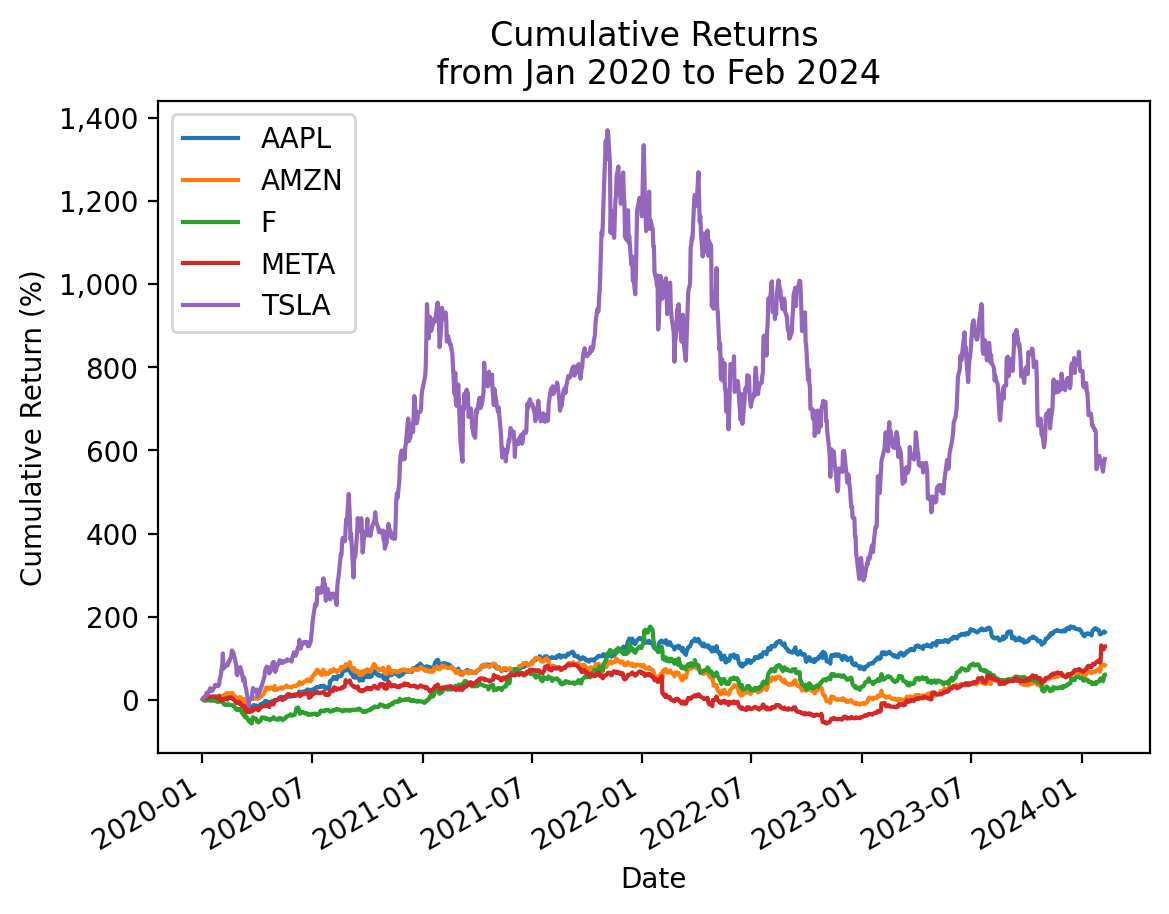
\includegraphics{herron_01_practice_04_files/figure-pdf/cell-16-output-1.png}

}

\end{figure}

\hypertarget{use-the-.cumsum-method-with-log-returns-to-plot-cumulative-returns-for-these-stocks-in-the-2020s-2}{%
\subsection{\texorpdfstring{Use the \texttt{.cumsum()} method with log
returns to plot cumulative returns for these stocks in the
2020s}{Use the .cumsum() method with log returns to plot cumulative returns for these stocks in the 2020s}}\label{use-the-.cumsum-method-with-log-returns-to-plot-cumulative-returns-for-these-stocks-in-the-2020s-2}}

\textbf{\emph{The log of products is the sum of logs!}}

\begin{Shaded}
\begin{Highlighting}[]
\NormalTok{cumret\_cumsum }\OperatorTok{=}\NormalTok{ (}
\NormalTok{    returns\_2020s }\CommentTok{\# returns during the 2020s}
\NormalTok{    .pipe(np.log1p) }\CommentTok{\# convert simple returns to log returns}
\NormalTok{    .cumsum() }\CommentTok{\# compound all returns}
\NormalTok{    .pipe(np.expm1) }\CommentTok{\# convert log returns to simple returns}
\NormalTok{)}

\NormalTok{cumret\_cumsum.tail()}
\end{Highlighting}
\end{Shaded}

\begin{longtable}[]{@{}llllll@{}}
\toprule\noalign{}
& AAPL & AMZN & F & META & TSLA \\
Date & & & & & \\
\midrule\noalign{}
\endhead
\bottomrule\noalign{}
\endlastfoot
2024-02-02 & 1.5985 & 0.8596 & 0.5224 & 1.3142 & 5.7379 \\
2024-02-05 & 1.6241 & 0.8433 & 0.4535 & 1.2383 & 5.4922 \\
2024-02-06 & 1.6468 & 0.8308 & 0.5136 & 1.2154 & 5.6371 \\
2024-02-07 & 1.6483 & 0.8457 & 0.6052 & 1.2879 & 5.7260 \\
2024-02-08 & 1.6331 & 0.8383 & 0.6090 & 1.2899 & 5.7970 \\
\end{longtable}

\begin{Shaded}
\begin{Highlighting}[]
\NormalTok{np.allclose(cumret\_cumprod, cumret\_cumsum)}
\end{Highlighting}
\end{Shaded}

\begin{verbatim}
True
\end{verbatim}

\begin{Shaded}
\begin{Highlighting}[]
\NormalTok{cumret\_cumsum.mul(}\DecValTok{100}\NormalTok{).plot()}

\CommentTok{\# https://stackoverflow.com/questions/25973581/how{-}to{-}format{-}axis{-}number{-}format{-}to{-}thousands{-}with{-}a{-}comma}
\ImportTok{from}\NormalTok{ matplotlib }\ImportTok{import}\NormalTok{ ticker}
\NormalTok{plt.gca().get\_yaxis().set\_major\_formatter(ticker.FuncFormatter(}\KeywordTok{lambda}\NormalTok{ x, p: }\BuiltInTok{format}\NormalTok{(}\BuiltInTok{int}\NormalTok{(x), }\StringTok{\textquotesingle{},\textquotesingle{}}\NormalTok{)))}

\NormalTok{plt.ylabel(}\StringTok{\textquotesingle{}Cumulative Return (\%)\textquotesingle{}}\NormalTok{)}
\NormalTok{plt.title(}\SpecialStringTok{f\textquotesingle{}Cumulative Returns}\CharTok{\textbackslash{}n}\SpecialStringTok{ from }\SpecialCharTok{\{}\NormalTok{returns\_2020s}\SpecialCharTok{.}\NormalTok{index}\SpecialCharTok{.}\BuiltInTok{min}\NormalTok{()}\SpecialCharTok{:}\OperatorTok{\%}\NormalTok{b }\OperatorTok{\%}\NormalTok{Y}\SpecialCharTok{\}}\SpecialStringTok{ to }\SpecialCharTok{\{}\NormalTok{returns\_2020s}\SpecialCharTok{.}\NormalTok{index}\SpecialCharTok{.}\BuiltInTok{max}\NormalTok{()}\SpecialCharTok{:}\OperatorTok{\%}\NormalTok{b }\OperatorTok{\%}\NormalTok{Y}\SpecialCharTok{\}}\SpecialStringTok{\textquotesingle{}}\NormalTok{)}
\NormalTok{plt.show()}
\end{Highlighting}
\end{Shaded}

\begin{figure}[H]

{\centering 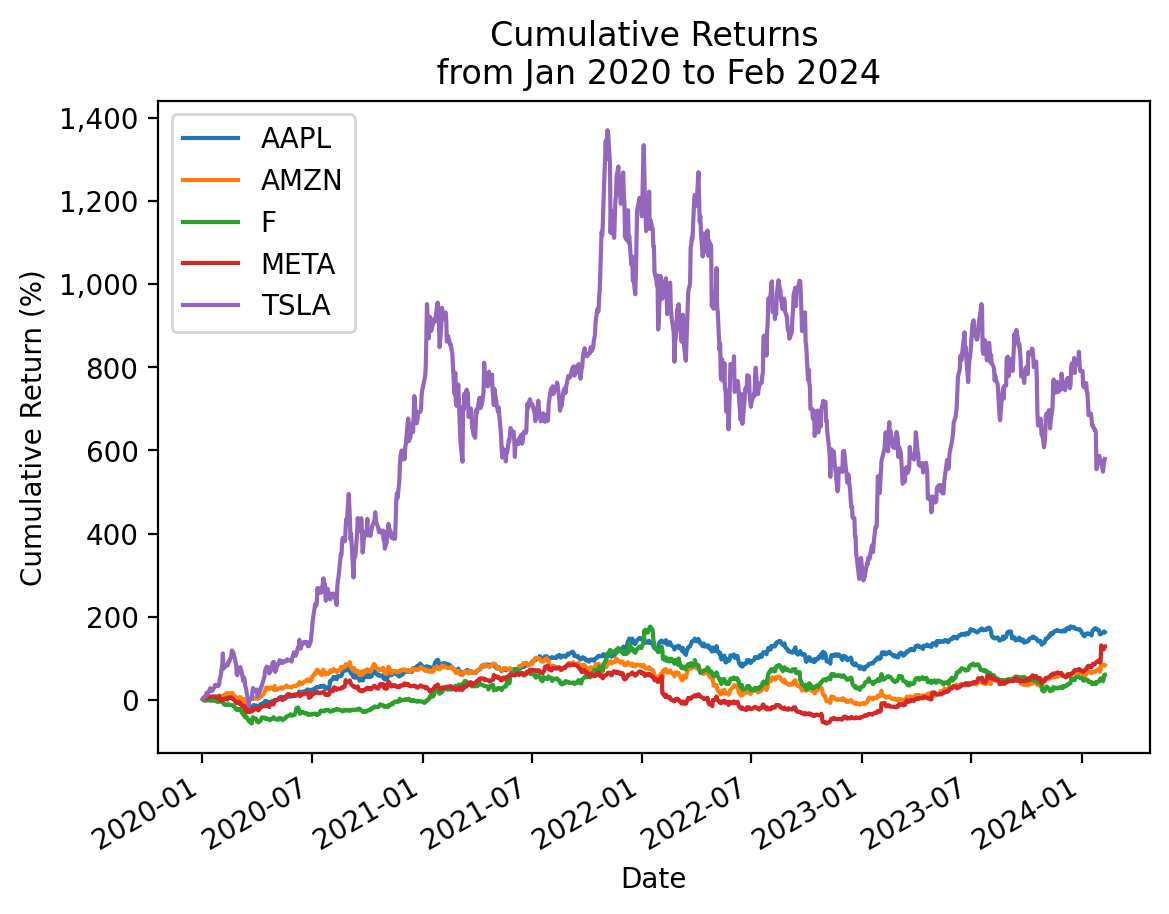
\includegraphics{herron_01_practice_04_files/figure-pdf/cell-19-output-1.png}

}

\end{figure}

\hypertarget{use-price-data-only-to-plot-cumulative-returns-for-these-stocks-in-the-2020s-2}{%
\subsection{Use price data only to plot cumulative returns for these
stocks in the
2020s}\label{use-price-data-only-to-plot-cumulative-returns-for-these-stocks-in-the-2020s-2}}

We can also calculate cumulative returns as the ratio of adjusted
closes. That is \(R_{0,T} = \frac{AC_T}{AC_0} - 1\). The trick here is
that \(FV_t = PV (1+r)^t\), so \((1+r)^t = \frac{FV_t}{PV}\).

\begin{Shaded}
\begin{Highlighting}[]
\NormalTok{returns\_2020s.iloc[}\DecValTok{0}\NormalTok{]}
\end{Highlighting}
\end{Shaded}

\begin{verbatim}
AAPL   0.0228
AMZN   0.0272
F      0.0129
META   0.0221
TSLA   0.0285
Name: 2020-01-02 00:00:00, dtype: float64
\end{verbatim}

\begin{Shaded}
\begin{Highlighting}[]
\NormalTok{cumret\_prices }\OperatorTok{=}\NormalTok{ prices[}\StringTok{\textquotesingle{}Adj Close\textquotesingle{}}\NormalTok{].loc[}\StringTok{\textquotesingle{}2020\textquotesingle{}}\NormalTok{:].iloc[:}\OperatorTok{{-}}\DecValTok{1}\NormalTok{] }\OperatorTok{/}\NormalTok{ prices[}\StringTok{\textquotesingle{}Adj Close\textquotesingle{}}\NormalTok{].loc[}\StringTok{\textquotesingle{}2019\textquotesingle{}}\NormalTok{].iloc[}\OperatorTok{{-}}\DecValTok{1}\NormalTok{] }\OperatorTok{{-}} \DecValTok{1}
\end{Highlighting}
\end{Shaded}

\begin{Shaded}
\begin{Highlighting}[]
\NormalTok{np.allclose(cumret\_prices, cumret\_cumprod)}
\end{Highlighting}
\end{Shaded}

\begin{verbatim}
True
\end{verbatim}

\hypertarget{calculate-the-sharpe-ratio-for-tsla-2}{%
\subsection{Calculate the Sharpe Ratio for
TSLA}\label{calculate-the-sharpe-ratio-for-tsla-2}}

Calculate the Sharpe Ratio with all available returns and 2020s returns.
Recall the Sharpe Ratio is \(\frac{\overline{r_i - r_f}}{\sigma_i}\),
where \(\sigma_i\) is the volatility of \emph{excess} returns.

\textbf{\emph{I suggest you write a function named
\texttt{calc\_sharpe()} to use for the rest of this notebook.}}

\begin{Shaded}
\begin{Highlighting}[]
\KeywordTok{def}\NormalTok{ calc\_sharpe(ri, rf}\OperatorTok{=}\NormalTok{ff[}\StringTok{\textquotesingle{}RF\textquotesingle{}}\NormalTok{], ppy}\OperatorTok{=}\DecValTok{252}\NormalTok{):}
\NormalTok{    ri\_rf }\OperatorTok{=}\NormalTok{ ri.sub(rf).dropna()}
    \ControlFlowTok{return}\NormalTok{ np.sqrt(ppy) }\OperatorTok{*}\NormalTok{ ri\_rf.mean() }\OperatorTok{/}\NormalTok{ ri\_rf.std()}
\end{Highlighting}
\end{Shaded}

\begin{Shaded}
\begin{Highlighting}[]
\NormalTok{calc\_sharpe(ri}\OperatorTok{=}\NormalTok{returns[}\StringTok{\textquotesingle{}TSLA\textquotesingle{}}\NormalTok{])}
\end{Highlighting}
\end{Shaded}

\begin{verbatim}
0.9261
\end{verbatim}

\begin{Shaded}
\begin{Highlighting}[]
\NormalTok{calc\_sharpe(ri}\OperatorTok{=}\NormalTok{returns\_2020s[}\StringTok{\textquotesingle{}TSLA\textquotesingle{}}\NormalTok{])}
\end{Highlighting}
\end{Shaded}

\begin{verbatim}
1.1212
\end{verbatim}

\textbf{\emph{Now we know about the \texttt{.pipe()} method, which lets
us ``convert'' functions into methods!}} We can use \texttt{.pipe()}
because \texttt{ri} is the first argument in \texttt{calc\_sharpe()}.

\begin{Shaded}
\begin{Highlighting}[]
\NormalTok{returns[}\StringTok{\textquotesingle{}TSLA\textquotesingle{}}\NormalTok{].pipe(calc\_sharpe)}
\end{Highlighting}
\end{Shaded}

\begin{verbatim}
0.9261
\end{verbatim}

\begin{Shaded}
\begin{Highlighting}[]
\NormalTok{returns\_2020s[}\StringTok{\textquotesingle{}TSLA\textquotesingle{}}\NormalTok{].pipe(calc\_sharpe)}
\end{Highlighting}
\end{Shaded}

\begin{verbatim}
1.1212
\end{verbatim}

\hypertarget{calculate-the-market-beta-for-tsla-2}{%
\subsection{Calculate the market beta for
TSLA}\label{calculate-the-market-beta-for-tsla-2}}

Calculate the market beta with all available returns and 2020s returns.
Recall we estimate market beta with the ordinary least squares (OLS)
regression \(R_i-R_f = \alpha + \beta (R_m-R_f) + \epsilon\). We can
estimate market beta with the covariance formula (i.e.,
\(\beta_i = \frac{Cov(R_i - R_f, R_m - R_f)}{Var(R_m-R_f)}\)) above for
a univariate regression if we do not need goodness of fit statistics.

\textbf{\emph{I suggest you write a function named \texttt{calc\_beta()}
to use for the rest of this notebook.}}

\begin{Shaded}
\begin{Highlighting}[]
\KeywordTok{def}\NormalTok{ calc\_beta(ri, rf}\OperatorTok{=}\NormalTok{ff[}\StringTok{\textquotesingle{}RF\textquotesingle{}}\NormalTok{], rm\_rf}\OperatorTok{=}\NormalTok{ff[}\StringTok{\textquotesingle{}Mkt{-}RF\textquotesingle{}}\NormalTok{]):}
\NormalTok{    ri\_rf }\OperatorTok{=}\NormalTok{ ri.sub(rf).dropna()}
    \ControlFlowTok{return}\NormalTok{ ri\_rf.cov(rm\_rf) }\OperatorTok{/}\NormalTok{ rm\_rf.loc[ri\_rf.index].var()}
\end{Highlighting}
\end{Shaded}

\begin{Shaded}
\begin{Highlighting}[]
\NormalTok{calc\_beta(ri}\OperatorTok{=}\NormalTok{returns[}\StringTok{\textquotesingle{}TSLA\textquotesingle{}}\NormalTok{])}
\end{Highlighting}
\end{Shaded}

\begin{verbatim}
1.4417
\end{verbatim}

\begin{Shaded}
\begin{Highlighting}[]
\NormalTok{calc\_beta(ri}\OperatorTok{=}\NormalTok{returns\_2020s[}\StringTok{\textquotesingle{}TSLA\textquotesingle{}}\NormalTok{])}
\end{Highlighting}
\end{Shaded}

\begin{verbatim}
1.5780
\end{verbatim}

\hypertarget{guess-the-sharpe-ratios-for-these-stocks-in-the-2020s-2}{%
\subsection{Guess the Sharpe Ratios for these stocks in the
2020s}\label{guess-the-sharpe-ratios-for-these-stocks-in-the-2020s-2}}

\hypertarget{guess-the-market-betas-for-these-stocks-in-the-2020s-2}{%
\subsection{Guess the market betas for these stocks in the
2020s}\label{guess-the-market-betas-for-these-stocks-in-the-2020s-2}}

\hypertarget{calculate-the-sharpe-ratios-for-these-stocks-in-the-2020s-2}{%
\subsection{Calculate the Sharpe Ratios for these stocks in the
2020s}\label{calculate-the-sharpe-ratios-for-these-stocks-in-the-2020s-2}}

How good were your guesses?

\begin{Shaded}
\begin{Highlighting}[]
\ControlFlowTok{for}\NormalTok{ i }\KeywordTok{in}\NormalTok{ returns\_2020s:}
\NormalTok{    sharpe\_i }\OperatorTok{=}\NormalTok{ returns\_2020s[i].pipe(calc\_sharpe)}
    \BuiltInTok{print}\NormalTok{(}\SpecialStringTok{f\textquotesingle{}Sharpe Ratio for }\SpecialCharTok{\{}\NormalTok{i}\SpecialCharTok{\}}\SpecialStringTok{:}\CharTok{\textbackslash{}t}\SpecialStringTok{ }\SpecialCharTok{\{}\NormalTok{sharpe\_i}\SpecialCharTok{:0.2f\}}\SpecialStringTok{\textquotesingle{}}\NormalTok{)}
\end{Highlighting}
\end{Shaded}

\begin{verbatim}
Sharpe Ratio for AAPL:   0.86
Sharpe Ratio for AMZN:   0.48
Sharpe Ratio for F:  0.42
Sharpe Ratio for META:   0.49
Sharpe Ratio for TSLA:   1.12
\end{verbatim}

We can also use pandas notation to vectorize this calculation. First
calculate \emph{excess} returns as \(r_i - r_f\).

\begin{Shaded}
\begin{Highlighting}[]
\NormalTok{returns\_2020s\_excess }\OperatorTok{=}\NormalTok{ returns\_2020s.sub(ff[}\StringTok{\textquotesingle{}RF\textquotesingle{}}\NormalTok{], axis}\OperatorTok{=}\DecValTok{0}\NormalTok{).dropna()}
\end{Highlighting}
\end{Shaded}

Then use pandas notation to calculate means, standard deviations, and
annualize.

\begin{Shaded}
\begin{Highlighting}[]
\NormalTok{(}
\NormalTok{    returns\_2020s\_excess}
\NormalTok{    .mean()}
\NormalTok{    .div(returns\_2020s\_excess.std())}
\NormalTok{    .mul(np.sqrt(}\DecValTok{252}\NormalTok{))}
\NormalTok{)}
\end{Highlighting}
\end{Shaded}

\begin{verbatim}
AAPL   0.8576
AMZN   0.4750
F      0.4240
META   0.4949
TSLA   1.1212
dtype: float64
\end{verbatim}

\textbf{\emph{Note:}} In a few weeks we will learn the \texttt{.apply()}
method, which avoids the loop syntax.

\begin{Shaded}
\begin{Highlighting}[]
\NormalTok{returns\_2020s.}\BuiltInTok{apply}\NormalTok{(calc\_sharpe)}
\end{Highlighting}
\end{Shaded}

\begin{verbatim}
AAPL   0.8576
AMZN   0.4750
F      0.4240
META   0.4949
TSLA   1.1212
dtype: float64
\end{verbatim}

\hypertarget{calculate-the-market-betas-for-these-stocks-in-the-2020s-2}{%
\subsection{Calculate the market betas for these stocks in the
2020s}\label{calculate-the-market-betas-for-these-stocks-in-the-2020s-2}}

How good were your guesses?

\begin{Shaded}
\begin{Highlighting}[]
\ControlFlowTok{for}\NormalTok{ i }\KeywordTok{in}\NormalTok{ returns\_2020s:}
\NormalTok{    beta\_i }\OperatorTok{=}\NormalTok{ returns\_2020s[i].pipe(calc\_beta)}
    \BuiltInTok{print}\NormalTok{(}\SpecialStringTok{f\textquotesingle{}Beta for }\SpecialCharTok{\{}\NormalTok{i}\SpecialCharTok{\}}\SpecialStringTok{:}\CharTok{\textbackslash{}t}\SpecialStringTok{ }\SpecialCharTok{\{}\NormalTok{beta\_i}\SpecialCharTok{:0.2f\}}\SpecialStringTok{\textquotesingle{}}\NormalTok{)}
\end{Highlighting}
\end{Shaded}

\begin{verbatim}
Beta for AAPL:   1.15
Beta for AMZN:   1.04
Beta for F:  1.22
Beta for META:   1.27
Beta for TSLA:   1.58
\end{verbatim}

Or we can follow out approach above to vectorize this calculation.
First, we need to add a market excess return column to
\texttt{returns\_2020s\_excess}.

\begin{Shaded}
\begin{Highlighting}[]
\NormalTok{returns\_2020s\_excess[}\StringTok{\textquotesingle{}Mkt{-}RF\textquotesingle{}}\NormalTok{] }\OperatorTok{=}\NormalTok{ ff[}\StringTok{\textquotesingle{}Mkt{-}RF\textquotesingle{}}\NormalTok{]}
\NormalTok{returns\_2020s\_excess.head()}
\end{Highlighting}
\end{Shaded}

\begin{longtable}[]{@{}lllllll@{}}
\toprule\noalign{}
& AAPL & AMZN & F & META & TSLA & Mkt-RF \\
Date & & & & & & \\
\midrule\noalign{}
\endhead
\bottomrule\noalign{}
\endlastfoot
2020-01-02 & 0.0228 & 0.0271 & 0.0128 & 0.0220 & 0.0285 & 0.0086 \\
2020-01-03 & -0.0098 & -0.0122 & -0.0224 & -0.0054 & 0.0296 & -0.0067 \\
2020-01-06 & 0.0079 & 0.0148 & -0.0055 & 0.0188 & 0.0192 & 0.0036 \\
2020-01-07 & -0.0048 & 0.0020 & 0.0098 & 0.0021 & 0.0387 & -0.0019 \\
2020-01-08 & 0.0160 & -0.0079 & -0.0001 & 0.0101 & 0.0491 & 0.0047 \\
\end{longtable}

\begin{Shaded}
\begin{Highlighting}[]
\NormalTok{vcv }\OperatorTok{=}\NormalTok{ returns\_2020s\_excess.cov()}
\NormalTok{vcv}
\end{Highlighting}
\end{Shaded}

\begin{longtable}[]{@{}lllllll@{}}
\toprule\noalign{}
& AAPL & AMZN & F & META & TSLA & Mkt-RF \\
\midrule\noalign{}
\endhead
\bottomrule\noalign{}
\endlastfoot
AAPL & 0.0004 & 0.0003 & 0.0002 & 0.0004 & 0.0005 & 0.0003 \\
AMZN & 0.0003 & 0.0006 & 0.0002 & 0.0004 & 0.0005 & 0.0002 \\
F & 0.0002 & 0.0002 & 0.0009 & 0.0003 & 0.0005 & 0.0003 \\
META & 0.0004 & 0.0004 & 0.0003 & 0.0009 & 0.0005 & 0.0003 \\
TSLA & 0.0005 & 0.0005 & 0.0005 & 0.0005 & 0.0018 & 0.0003 \\
Mkt-RF & 0.0003 & 0.0002 & 0.0003 & 0.0003 & 0.0003 & 0.0002 \\
\end{longtable}

\begin{Shaded}
\begin{Highlighting}[]
\NormalTok{vcv[}\StringTok{\textquotesingle{}Mkt{-}RF\textquotesingle{}}\NormalTok{].div(vcv.loc[}\StringTok{\textquotesingle{}Mkt{-}RF\textquotesingle{}}\NormalTok{, }\StringTok{\textquotesingle{}Mkt{-}RF\textquotesingle{}}\NormalTok{]).plot(kind}\OperatorTok{=}\StringTok{\textquotesingle{}bar\textquotesingle{}}\NormalTok{)}
\NormalTok{plt.xlabel(}\StringTok{\textquotesingle{}Ticker\textquotesingle{}}\NormalTok{)}
\NormalTok{plt.ylabel(}\StringTok{\textquotesingle{}CAPM Beta\textquotesingle{}}\NormalTok{)}
\NormalTok{plt.title(}\StringTok{\textquotesingle{}CAPM Betas\textquotesingle{}}\NormalTok{)}
\NormalTok{plt.show()}
\end{Highlighting}
\end{Shaded}

\begin{figure}[H]

{\centering \includegraphics{herron_01_practice_04_files/figure-pdf/cell-39-output-1.png}

}

\end{figure}

\textbf{\emph{Note:}} In a few weeks we will learn the \texttt{.apply()}
method, which avoids the loop syntax.

\begin{Shaded}
\begin{Highlighting}[]
\NormalTok{returns\_2020s.}\BuiltInTok{apply}\NormalTok{(calc\_beta)}
\end{Highlighting}
\end{Shaded}

\begin{verbatim}
AAPL   1.1541
AMZN   1.0429
F      1.2231
META   1.2710
TSLA   1.5780
dtype: float64
\end{verbatim}

\hypertarget{calculate-the-sharpe-ratio-for-an-equally-weighted-portfolio-of-these-stocks-in-the-2020s-2}{%
\subsection{\texorpdfstring{Calculate the Sharpe Ratio for an
\emph{equally weighted} portfolio of these stocks in the
2020s}{Calculate the Sharpe Ratio for an equally weighted portfolio of these stocks in the 2020s}}\label{calculate-the-sharpe-ratio-for-an-equally-weighted-portfolio-of-these-stocks-in-the-2020s-2}}

What do you notice?

\begin{Shaded}
\begin{Highlighting}[]
\NormalTok{returns\_2020s.mean(axis}\OperatorTok{=}\DecValTok{1}\NormalTok{).pipe(calc\_sharpe)}
\end{Highlighting}
\end{Shaded}

\begin{verbatim}
0.9573
\end{verbatim}

Because diversification reduces portfolio standard deviation less than
the sum of its parts, the Sharpe Ratio of the equally weighted portfolio
is less than the equally weighted mean of the single-stock Sharpe
Ratios.

\begin{Shaded}
\begin{Highlighting}[]
\NormalTok{returns\_2020s.}\BuiltInTok{apply}\NormalTok{(calc\_sharpe).mean()}
\end{Highlighting}
\end{Shaded}

\begin{verbatim}
0.6745
\end{verbatim}

\hypertarget{calculate-the-market-beta-for-an-equally-weighted-portfolio-of-these-stocks-in-the-2020s-2}{%
\subsection{\texorpdfstring{Calculate the market beta for an
\emph{equally weighted} portfolio of these stocks in the
2020s}{Calculate the market beta for an equally weighted portfolio of these stocks in the 2020s}}\label{calculate-the-market-beta-for-an-equally-weighted-portfolio-of-these-stocks-in-the-2020s-2}}

What do you notice?

Beta measures \emph{non}diversifiable risk, so
\(\beta_P = \sum w_i \beta_i\)!

\begin{Shaded}
\begin{Highlighting}[]
\NormalTok{returns\_2020s.mean(axis}\OperatorTok{=}\DecValTok{1}\NormalTok{).pipe(calc\_beta)}
\end{Highlighting}
\end{Shaded}

\begin{verbatim}
1.2538
\end{verbatim}

\begin{Shaded}
\begin{Highlighting}[]
\NormalTok{returns\_2020s.}\BuiltInTok{apply}\NormalTok{(calc\_beta).mean()}
\end{Highlighting}
\end{Shaded}

\begin{verbatim}
1.2538
\end{verbatim}

\hypertarget{calculate-the-market-betas-for-these-stocks-every-calendar-year-for-every-possible-year-2}{%
\subsection{Calculate the market betas for these stocks every calendar
year for every possible
year}\label{calculate-the-market-betas-for-these-stocks-every-calendar-year-for-every-possible-year-2}}

Save these market betas to data frame \texttt{betas}. Our current Python
knowledge limits us to a for-loop, but we will learn easier and faster
approaches soon!

\begin{Shaded}
\begin{Highlighting}[]
\NormalTok{betas }\OperatorTok{=}\NormalTok{ pd.DataFrame(}
\NormalTok{    index}\OperatorTok{=}\BuiltInTok{range}\NormalTok{(}\DecValTok{1972}\NormalTok{, }\DecValTok{2024}\NormalTok{),}
\NormalTok{    columns}\OperatorTok{=}\NormalTok{returns.columns}
\NormalTok{)}

\NormalTok{betas.columns.name }\OperatorTok{=} \StringTok{\textquotesingle{}Ticker\textquotesingle{}}
\NormalTok{betas.index.name }\OperatorTok{=} \StringTok{\textquotesingle{}Year\textquotesingle{}}

\NormalTok{betas.tail()}
\end{Highlighting}
\end{Shaded}

\begin{longtable}[]{@{}llllll@{}}
\toprule\noalign{}
Ticker & AAPL & AMZN & F & META & TSLA \\
Year & & & & & \\
\midrule\noalign{}
\endhead
\bottomrule\noalign{}
\endlastfoot
2019 & NaN & NaN & NaN & NaN & NaN \\
2020 & NaN & NaN & NaN & NaN & NaN \\
2021 & NaN & NaN & NaN & NaN & NaN \\
2022 & NaN & NaN & NaN & NaN & NaN \\
2023 & NaN & NaN & NaN & NaN & NaN \\
\end{longtable}

\begin{Shaded}
\begin{Highlighting}[]
\ControlFlowTok{for}\NormalTok{ i }\KeywordTok{in}\NormalTok{ betas.index: }
    \ControlFlowTok{for}\NormalTok{ c }\KeywordTok{in}\NormalTok{ betas.columns:}
\NormalTok{        betas.at[i, c] }\OperatorTok{=}\NormalTok{ returns.loc[}\BuiltInTok{str}\NormalTok{(i), c].pipe(calc\_beta)}

\NormalTok{betas.tail()}
\end{Highlighting}
\end{Shaded}

\begin{longtable}[]{@{}llllll@{}}
\toprule\noalign{}
Ticker & AAPL & AMZN & F & META & TSLA \\
Year & & & & & \\
\midrule\noalign{}
\endhead
\bottomrule\noalign{}
\endlastfoot
2019 & 1.4751 & 1.2752 & 1.0733 & 1.2094 & 1.3262 \\
2020 & 1.1174 & 0.6866 & 1.1052 & 0.9913 & 1.3041 \\
2021 & 1.1957 & 0.9822 & 1.2396 & 1.2014 & 1.9891 \\
2022 & 1.2386 & 1.5922 & 1.3824 & 1.6843 & 1.7414 \\
2023 & 1.0369 & 1.4649 & 1.3947 & 1.6630 & 2.2218 \\
\end{longtable}

\hypertarget{plot-the-time-series-of-market-betas-2}{%
\subsection{Plot the time series of market
betas}\label{plot-the-time-series-of-market-betas-2}}

\begin{Shaded}
\begin{Highlighting}[]
\NormalTok{betas.plot()}
\NormalTok{plt.ylabel(}\StringTok{\textquotesingle{}CAPM Beta\textquotesingle{}}\NormalTok{)}
\NormalTok{plt.title(}\StringTok{\textquotesingle{}CAPM Betas\textquotesingle{}}\NormalTok{)}
\NormalTok{plt.show()}
\end{Highlighting}
\end{Shaded}

\begin{figure}[H]

{\centering 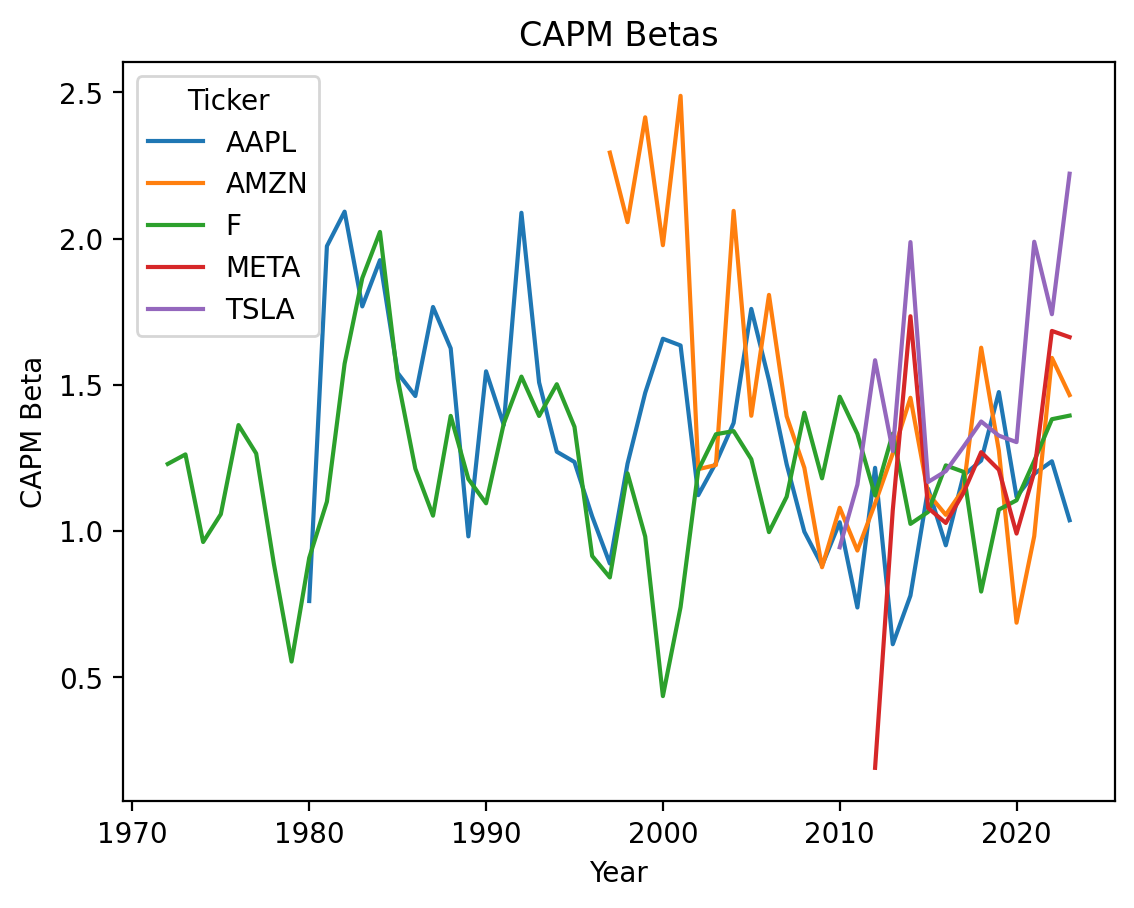
\includegraphics{herron_01_practice_04_files/figure-pdf/cell-47-output-1.png}

}

\end{figure}

\hypertarget{herron-topic-1---practice-for-section-05}{%
\chapter{Herron Topic 1 - Practice for Section
05}\label{herron-topic-1---practice-for-section-05}}

\hypertarget{announcements-19}{%
\section{Announcements}\label{announcements-19}}

\begin{enumerate}
\def\labelenumi{\arabic{enumi}.}
\tightlist
\item
  DataCamp

  \begin{enumerate}
  \def\labelenumii{\arabic{enumii}.}
  \tightlist
  \item
    \emph{Data Manipulation with pandas} due by Friday, 2/9, at 11:59 PM
  \item
    \emph{Joining Data with pandas} due by Friday, 2/16, at 11:59 PM
  \item
    \emph{Earn 10,000 XP} due by Friday, 3/15, at 11:59 PM
  \end{enumerate}
\item
  I posted Project 1 to Canvas

  \begin{enumerate}
  \def\labelenumii{\arabic{enumii}.}
  \tightlist
  \item
    Slides and notebook due by Friday, 2/23, at 11:59 PM
  \item
    Keep joining teams and let me know if you need help
  \end{enumerate}
\end{enumerate}

\hypertarget{minute-recap-18}{%
\section{10-Minute Recap}\label{minute-recap-18}}

\begin{Shaded}
\begin{Highlighting}[]
\ImportTok{import}\NormalTok{ matplotlib.pyplot }\ImportTok{as}\NormalTok{ plt}
\ImportTok{import}\NormalTok{ numpy }\ImportTok{as}\NormalTok{ np}
\ImportTok{import}\NormalTok{ pandas }\ImportTok{as}\NormalTok{ pd}
\ImportTok{import}\NormalTok{ pandas\_datareader }\ImportTok{as}\NormalTok{ pdr}
\ImportTok{import}\NormalTok{ yfinance }\ImportTok{as}\NormalTok{ yf}
\end{Highlighting}
\end{Shaded}

\begin{Shaded}
\begin{Highlighting}[]
\OperatorTok{\%}\NormalTok{precision }\DecValTok{4}
\NormalTok{pd.options.display.float\_format }\OperatorTok{=} \StringTok{\textquotesingle{}}\SpecialCharTok{\{:.4f\}}\StringTok{\textquotesingle{}}\NormalTok{.}\BuiltInTok{format}
\OperatorTok{\%}\NormalTok{config InlineBackend.figure\_format }\OperatorTok{=} \StringTok{\textquotesingle{}retina\textquotesingle{}}
\end{Highlighting}
\end{Shaded}

First, we will use two packages to download data from the Web:

\begin{enumerate}
\def\labelenumi{\arabic{enumi}.}
\tightlist
\item
  \texttt{yfinance} for Yahoo! Finance
\item
  \texttt{pandas-datareader} for Ken French (and FRED and many others)
\end{enumerate}

Second, there are ``simple returns'' and ``log returns''

\begin{enumerate}
\def\labelenumi{\arabic{enumi}.}
\tightlist
\item
  Simple returns are the returns that investors receive that we learned
  in FINA 6331 and FINA 6333:
  \(r_t = \frac{p_t + d_t - p_{t-1}}{p_{t-1}}\)
\item
  Log returns are the log of one plus simple returns. Why do we use
  them?

  \begin{enumerate}
  \def\labelenumii{\arabic{enumii}.}
  \tightlist
  \item
    \textbf{\emph{Log returns are additive}}, while simple returns are
    multiplicative. This additive property makes math really easy with
    log returns:
    \(\log(\prod_{t=0}^T (1 + r_t)) = \sum_{t=0}^T \log(1+r_t)\), so
    \(r_{0,T} = \prod_{t=0}^T (1 + r_t) - 1 = e^{\sum_{t=0}^T \log(1+r_t)} - 1\)
  \item
    \textbf{\emph{Log returns are almost normally distributed}}
  \end{enumerate}
\end{enumerate}

\textbf{\emph{We will almost always use simple returns.}} The exeception
is time-consuming calculations, which we will often do in log returns to
save us time.

Third, we can calculate portfolio returns a few ways!

\begin{enumerate}
\def\labelenumi{\arabic{enumi}.}
\tightlist
\item
  \texttt{returns.mean(axis=1)} is \emph{equally-weighted} portfolio
  returns, rebalanced at the same frequency as the returns (i.e.,
  rebalanced every return period)
\item
  \texttt{returns.dot(weights)} lets us use any weights in the
  \texttt{weights} array, rebalanced at the same frequency as the
  returns
\end{enumerate}

\hypertarget{practice-19}{%
\section{Practice}\label{practice-19}}

\hypertarget{download-all-available-daily-price-data-for-tickers-tsla-f-aapl-amzn-and-meta-to-data-frame-prices-3}{%
\subsection{\texorpdfstring{Download all available daily price data for
tickers TSLA, F, AAPL, AMZN, and META to data frame
\texttt{prices}}{Download all available daily price data for tickers TSLA, F, AAPL, AMZN, and META to data frame prices}}\label{download-all-available-daily-price-data-for-tickers-tsla-f-aapl-amzn-and-meta-to-data-frame-prices-3}}

\begin{Shaded}
\begin{Highlighting}[]
\NormalTok{tickers }\OperatorTok{=} \StringTok{\textquotesingle{}TSLA F AAPL AMZN META\textquotesingle{}}
\NormalTok{prices }\OperatorTok{=}\NormalTok{ yf.download(tickers}\OperatorTok{=}\NormalTok{tickers)}
\end{Highlighting}
\end{Shaded}

\begin{verbatim}
[*********************100%%**********************]  5 of 5 completed
\end{verbatim}

\begin{Shaded}
\begin{Highlighting}[]
\NormalTok{prices.head()}
\end{Highlighting}
\end{Shaded}

\begin{longtable}[]{@{}llllllllllllllllllllll@{}}
\toprule\noalign{}
&
\multicolumn{5}{>{\raggedright\arraybackslash}p{(\columnwidth - 42\tabcolsep) * \real{0.0000} + 8\tabcolsep}}{%
Adj Close} &
\multicolumn{5}{>{\raggedright\arraybackslash}p{(\columnwidth - 42\tabcolsep) * \real{0.0000} + 8\tabcolsep}}{%
Close} & ... &
\multicolumn{5}{>{\raggedright\arraybackslash}p{(\columnwidth - 42\tabcolsep) * \real{0.0000} + 8\tabcolsep}}{%
Open} &
\multicolumn{5}{>{\raggedright\arraybackslash}p{(\columnwidth - 42\tabcolsep) * \real{0.0000} + 8\tabcolsep}@{}}{%
Volume} \\
& AAPL & AMZN & F & META & TSLA & AAPL & AMZN & F & META & TSLA & ... &
AAPL & AMZN & F & META & TSLA & AAPL & AMZN & F & META & TSLA \\
Date & & & & & & & & & & & & & & & & & & & & & \\
\midrule\noalign{}
\endhead
\bottomrule\noalign{}
\endlastfoot
1972-06-01 & NaN & NaN & 0.2419 & NaN & NaN & NaN & NaN & 2.1532 & NaN &
NaN & ... & NaN & NaN & 0.0000 & NaN & NaN & NaN & NaN & 1091238 & NaN &
NaN \\
1972-06-02 & NaN & NaN & 0.2414 & NaN & NaN & NaN & NaN & 2.1492 & NaN &
NaN & ... & NaN & NaN & 2.1532 & NaN & NaN & NaN & NaN & 1174468 & NaN &
NaN \\
1972-06-05 & NaN & NaN & 0.2414 & NaN & NaN & NaN & NaN & 2.1492 & NaN &
NaN & ... & NaN & NaN & 2.1492 & NaN & NaN & NaN & NaN & 5209582 & NaN &
NaN \\
1972-06-06 & NaN & NaN & 0.2387 & NaN & NaN & NaN & NaN & 2.1248 & NaN &
NaN & ... & NaN & NaN & 2.1492 & NaN & NaN & NaN & NaN & 1424158 & NaN &
NaN \\
1972-06-07 & NaN & NaN & 0.2373 & NaN & NaN & NaN & NaN & 2.1127 & NaN &
NaN & ... & NaN & NaN & 2.1248 & NaN & NaN & NaN & NaN & 675088 & NaN &
NaN \\
\end{longtable}

\hypertarget{calculate-all-available-daily-returns-and-save-to-data-frame-returns-4}{%
\subsection{\texorpdfstring{Calculate all available daily returns and
save to data frame
\texttt{returns}}{Calculate all available daily returns and save to data frame returns}}\label{calculate-all-available-daily-returns-and-save-to-data-frame-returns-4}}

\begin{Shaded}
\begin{Highlighting}[]
\NormalTok{returns }\OperatorTok{=}\NormalTok{ (}
\NormalTok{    prices[}\StringTok{\textquotesingle{}Adj Close\textquotesingle{}}\NormalTok{] }\CommentTok{\# slice adj close}
\NormalTok{    .iloc[:}\OperatorTok{{-}}\DecValTok{1}\NormalTok{] }\CommentTok{\# drop the last price because it might be intraday (i.e., not a close)}
\NormalTok{    .pct\_change() }\CommentTok{\# calculate simple returns}
\NormalTok{)}

\NormalTok{returns}
\end{Highlighting}
\end{Shaded}

\begin{longtable}[]{@{}llllll@{}}
\toprule\noalign{}
& AAPL & AMZN & F & META & TSLA \\
Date & & & & & \\
\midrule\noalign{}
\endhead
\bottomrule\noalign{}
\endlastfoot
1972-06-01 & NaN & NaN & NaN & NaN & NaN \\
1972-06-02 & NaN & NaN & -0.0019 & NaN & NaN \\
1972-06-05 & NaN & NaN & 0.0000 & NaN & NaN \\
1972-06-06 & NaN & NaN & -0.0113 & NaN & NaN \\
1972-06-07 & NaN & NaN & -0.0057 & NaN & NaN \\
... & ... & ... & ... & ... & ... \\
2024-02-02 & -0.0054 & 0.0787 & 0.0033 & 0.2032 & -0.0050 \\
2024-02-05 & 0.0098 & -0.0087 & -0.0453 & -0.0328 & -0.0365 \\
2024-02-06 & 0.0086 & -0.0068 & 0.0414 & -0.0102 & 0.0223 \\
2024-02-07 & 0.0006 & 0.0082 & 0.0605 & 0.0327 & 0.0134 \\
2024-02-08 & -0.0058 & -0.0040 & 0.0023 & 0.0009 & 0.0106 \\
\end{longtable}

\hypertarget{slices-returns-for-the-2020s-and-assign-to-returns_2020s-3}{%
\subsection{\texorpdfstring{Slices returns for the 2020s and assign to
\texttt{returns\_2020s}}{Slices returns for the 2020s and assign to returns\_2020s}}\label{slices-returns-for-the-2020s-and-assign-to-returns_2020s-3}}

\begin{Shaded}
\begin{Highlighting}[]
\NormalTok{returns\_2020s }\OperatorTok{=}\NormalTok{ returns.loc[}\StringTok{\textquotesingle{}2020\textquotesingle{}}\NormalTok{:] }\CommentTok{\# always use an unambiguos date format, like YYYY{-}MM{-}DD}

\NormalTok{returns\_2020s}
\end{Highlighting}
\end{Shaded}

\begin{longtable}[]{@{}llllll@{}}
\toprule\noalign{}
& AAPL & AMZN & F & META & TSLA \\
Date & & & & & \\
\midrule\noalign{}
\endhead
\bottomrule\noalign{}
\endlastfoot
2020-01-02 & 0.0228 & 0.0272 & 0.0129 & 0.0221 & 0.0285 \\
2020-01-03 & -0.0097 & -0.0121 & -0.0223 & -0.0053 & 0.0296 \\
2020-01-06 & 0.0080 & 0.0149 & -0.0054 & 0.0188 & 0.0193 \\
2020-01-07 & -0.0047 & 0.0021 & 0.0098 & 0.0022 & 0.0388 \\
2020-01-08 & 0.0161 & -0.0078 & 0.0000 & 0.0101 & 0.0492 \\
... & ... & ... & ... & ... & ... \\
2024-02-02 & -0.0054 & 0.0787 & 0.0033 & 0.2032 & -0.0050 \\
2024-02-05 & 0.0098 & -0.0087 & -0.0453 & -0.0328 & -0.0365 \\
2024-02-06 & 0.0086 & -0.0068 & 0.0414 & -0.0102 & 0.0223 \\
2024-02-07 & 0.0006 & 0.0082 & 0.0605 & 0.0327 & 0.0134 \\
2024-02-08 & -0.0058 & -0.0040 & 0.0023 & 0.0009 & 0.0106 \\
\end{longtable}

\hypertarget{download-all-available-data-for-the-fama-and-french-daily-benchmark-factors-to-dictionary-ff_all-3}{%
\subsection{\texorpdfstring{Download all available data for the Fama and
French daily benchmark factors to dictionary
\texttt{ff\_all}}{Download all available data for the Fama and French daily benchmark factors to dictionary ff\_all}}\label{download-all-available-data-for-the-fama-and-french-daily-benchmark-factors-to-dictionary-ff_all-3}}

I often use the following code snippet to find the exact name for the
the daily benchmark factors file.

\begin{Shaded}
\begin{Highlighting}[]
\NormalTok{pdr.famafrench.get\_available\_datasets()[:}\DecValTok{5}\NormalTok{]}
\end{Highlighting}
\end{Shaded}

\begin{verbatim}
['F-F_Research_Data_Factors',
 'F-F_Research_Data_Factors_weekly',
 'F-F_Research_Data_Factors_daily',
 'F-F_Research_Data_5_Factors_2x3',
 'F-F_Research_Data_5_Factors_2x3_daily']
\end{verbatim}

\begin{Shaded}
\begin{Highlighting}[]
\NormalTok{ff\_all }\OperatorTok{=}\NormalTok{ pdr.DataReader(}
\NormalTok{    name}\OperatorTok{=}\StringTok{\textquotesingle{}F{-}F\_Research\_Data\_Factors\_daily\textquotesingle{}}\NormalTok{,}
\NormalTok{    data\_source}\OperatorTok{=}\StringTok{\textquotesingle{}famafrench\textquotesingle{}}\NormalTok{,}
\NormalTok{    start}\OperatorTok{=}\StringTok{\textquotesingle{}1900\textquotesingle{}} \CommentTok{\# most data start in 1926{-}07{-}01, but 1900 is easier to remember and type}
\NormalTok{)}
\end{Highlighting}
\end{Shaded}

\begin{verbatim}
C:\Users\r.herron\AppData\Local\Temp\ipykernel_27720\4231759426.py:1: FutureWarning: The argument 'date_parser' is deprecated and will be removed in a future version. Please use 'date_format' instead, or read your data in as 'object' dtype and then call 'to_datetime'.
  ff_all = pdr.DataReader(
\end{verbatim}

The \texttt{DESCR} key in the dictionary tells us about the data frames
that \texttt{pandas-datareader} returns.

\begin{Shaded}
\begin{Highlighting}[]
\BuiltInTok{print}\NormalTok{(ff\_all[}\StringTok{\textquotesingle{}DESCR\textquotesingle{}}\NormalTok{])}
\end{Highlighting}
\end{Shaded}

\begin{verbatim}
F-F Research Data Factors daily
-------------------------------

This file was created by CMPT_ME_BEME_RETS_DAILY using the 202312 CRSP database. The Tbill return is the simple daily rate that, over the number of trading days in the month, compounds to 1-month TBill rate from Ibbotson and Associates Inc. Copyright 2023 Kenneth R. French

  0 : (25649 rows x 4 cols)
\end{verbatim}

\hypertarget{slice-the-daily-benchmark-factors-convert-them-to-decimal-returns-and-assign-to-ff-3}{%
\subsection{\texorpdfstring{Slice the daily benchmark factors, convert
them to decimal returns, and assign to
\texttt{ff}}{Slice the daily benchmark factors, convert them to decimal returns, and assign to ff}}\label{slice-the-daily-benchmark-factors-convert-them-to-decimal-returns-and-assign-to-ff-3}}

\begin{Shaded}
\begin{Highlighting}[]
\NormalTok{ff }\OperatorTok{=}\NormalTok{ ff\_all[}\DecValTok{0}\NormalTok{].div(}\DecValTok{100}\NormalTok{)}

\NormalTok{ff}
\end{Highlighting}
\end{Shaded}

\begin{longtable}[]{@{}lllll@{}}
\toprule\noalign{}
& Mkt-RF & SMB & HML & RF \\
Date & & & & \\
\midrule\noalign{}
\endhead
\bottomrule\noalign{}
\endlastfoot
1926-07-01 & 0.0010 & -0.0025 & -0.0027 & 0.0001 \\
1926-07-02 & 0.0045 & -0.0033 & -0.0006 & 0.0001 \\
1926-07-06 & 0.0017 & 0.0030 & -0.0039 & 0.0001 \\
1926-07-07 & 0.0009 & -0.0058 & 0.0002 & 0.0001 \\
1926-07-08 & 0.0021 & -0.0038 & 0.0019 & 0.0001 \\
... & ... & ... & ... & ... \\
2023-12-22 & 0.0021 & 0.0064 & 0.0009 & 0.0002 \\
2023-12-26 & 0.0048 & 0.0069 & 0.0046 & 0.0002 \\
2023-12-27 & 0.0016 & 0.0014 & 0.0012 & 0.0002 \\
2023-12-28 & -0.0001 & -0.0036 & 0.0003 & 0.0002 \\
2023-12-29 & -0.0043 & -0.0112 & -0.0037 & 0.0002 \\
\end{longtable}

\hypertarget{use-the-.cumprod-method-to-plot-cumulative-returns-for-these-stocks-in-the-2020s-3}{%
\subsection{\texorpdfstring{Use the \texttt{.cumprod()} method to plot
cumulative returns for these stocks in the
2020s}{Use the .cumprod() method to plot cumulative returns for these stocks in the 2020s}}\label{use-the-.cumprod-method-to-plot-cumulative-returns-for-these-stocks-in-the-2020s-3}}

We use the \texttt{.prod()} method to calculate \emph{total} returns,
because
\(r_{total} = r_{0,T} = \left[ \prod_{t=0}^T (1 + r_t) \right] -1\).

\begin{Shaded}
\begin{Highlighting}[]
\NormalTok{(}
\NormalTok{    returns\_2020s }\CommentTok{\# returns during the 2020s}
\NormalTok{    .add(}\DecValTok{1}\NormalTok{) }\CommentTok{\# add 1 before we compound}
\NormalTok{    .prod() }\CommentTok{\# compound all returns}
\NormalTok{    .sub(}\DecValTok{1}\NormalTok{) }\CommentTok{\# subtract 1 to recover total returns}
\NormalTok{)}
\end{Highlighting}
\end{Shaded}

\begin{verbatim}
AAPL   1.6331
AMZN   0.8383
F      0.6090
META   1.2899
TSLA   5.7970
dtype: float64
\end{verbatim}

We use the \texttt{.cumprod()} to calculate \emph{cumulative} returns,
which are the total returns for every date between \(0\) and \(T\)
(i.e., \(r_{0,t} \forall t \in {0, 1, \ldots T}\))

\begin{Shaded}
\begin{Highlighting}[]
\NormalTok{cumret\_cumprod }\OperatorTok{=}\NormalTok{ (}
\NormalTok{    returns\_2020s }\CommentTok{\# returns during the 2020s}
\NormalTok{    .add(}\DecValTok{1}\NormalTok{) }\CommentTok{\# add 1 before we compound}
\NormalTok{    .cumprod() }\CommentTok{\# compound returns up to time t}
\NormalTok{    .sub(}\DecValTok{1}\NormalTok{) }\CommentTok{\# subtract 1 to recover cumulative return at time t}
\NormalTok{)}
\end{Highlighting}
\end{Shaded}

\begin{Shaded}
\begin{Highlighting}[]
\NormalTok{cumret\_cumprod}
\end{Highlighting}
\end{Shaded}

\begin{longtable}[]{@{}llllll@{}}
\toprule\noalign{}
& AAPL & AMZN & F & META & TSLA \\
Date & & & & & \\
\midrule\noalign{}
\endhead
\bottomrule\noalign{}
\endlastfoot
2020-01-02 & 0.0228 & 0.0272 & 0.0129 & 0.0221 & 0.0285 \\
2020-01-03 & 0.0129 & 0.0147 & -0.0097 & 0.0167 & 0.0590 \\
2020-01-06 & 0.0209 & 0.0298 & -0.0151 & 0.0358 & 0.0794 \\
2020-01-07 & 0.0161 & 0.0319 & -0.0054 & 0.0381 & 0.1213 \\
2020-01-08 & 0.0325 & 0.0239 & -0.0054 & 0.0486 & 0.1764 \\
... & ... & ... & ... & ... & ... \\
2024-02-02 & 1.5985 & 0.8596 & 0.5224 & 1.3142 & 5.7379 \\
2024-02-05 & 1.6241 & 0.8433 & 0.4535 & 1.2383 & 5.4922 \\
2024-02-06 & 1.6468 & 0.8308 & 0.5136 & 1.2154 & 5.6371 \\
2024-02-07 & 1.6483 & 0.8457 & 0.6052 & 1.2879 & 5.7260 \\
2024-02-08 & 1.6331 & 0.8383 & 0.6090 & 1.2899 & 5.7970 \\
\end{longtable}

\begin{Shaded}
\begin{Highlighting}[]
\NormalTok{cumret\_cumprod.mul(}\DecValTok{100}\NormalTok{).plot()}

\CommentTok{\# https://stackoverflow.com/questions/25973581/how{-}to{-}format{-}axis{-}number{-}format{-}to{-}thousands{-}with{-}a{-}comma}
\ImportTok{from}\NormalTok{ matplotlib }\ImportTok{import}\NormalTok{ ticker}
\NormalTok{plt.gca().get\_yaxis().set\_major\_formatter(ticker.FuncFormatter(}\KeywordTok{lambda}\NormalTok{ x, p: }\BuiltInTok{format}\NormalTok{(}\BuiltInTok{int}\NormalTok{(x), }\StringTok{\textquotesingle{},\textquotesingle{}}\NormalTok{)))}

\NormalTok{plt.ylabel(}\StringTok{\textquotesingle{}Cumulative Return (\%)\textquotesingle{}}\NormalTok{)}
\NormalTok{plt.title(}\SpecialStringTok{f\textquotesingle{}Cumulative Returns}\CharTok{\textbackslash{}n}\SpecialStringTok{ from }\SpecialCharTok{\{}\NormalTok{returns\_2020s}\SpecialCharTok{.}\NormalTok{index}\SpecialCharTok{.}\BuiltInTok{min}\NormalTok{()}\SpecialCharTok{:}\OperatorTok{\%}\NormalTok{b }\OperatorTok{\%}\NormalTok{Y}\SpecialCharTok{\}}\SpecialStringTok{ to }\SpecialCharTok{\{}\NormalTok{returns\_2020s}\SpecialCharTok{.}\NormalTok{index}\SpecialCharTok{.}\BuiltInTok{max}\NormalTok{()}\SpecialCharTok{:}\OperatorTok{\%}\NormalTok{b }\OperatorTok{\%}\NormalTok{Y}\SpecialCharTok{\}}\SpecialStringTok{\textquotesingle{}}\NormalTok{)}
\NormalTok{plt.show()}
\end{Highlighting}
\end{Shaded}

\begin{figure}[H]

{\centering 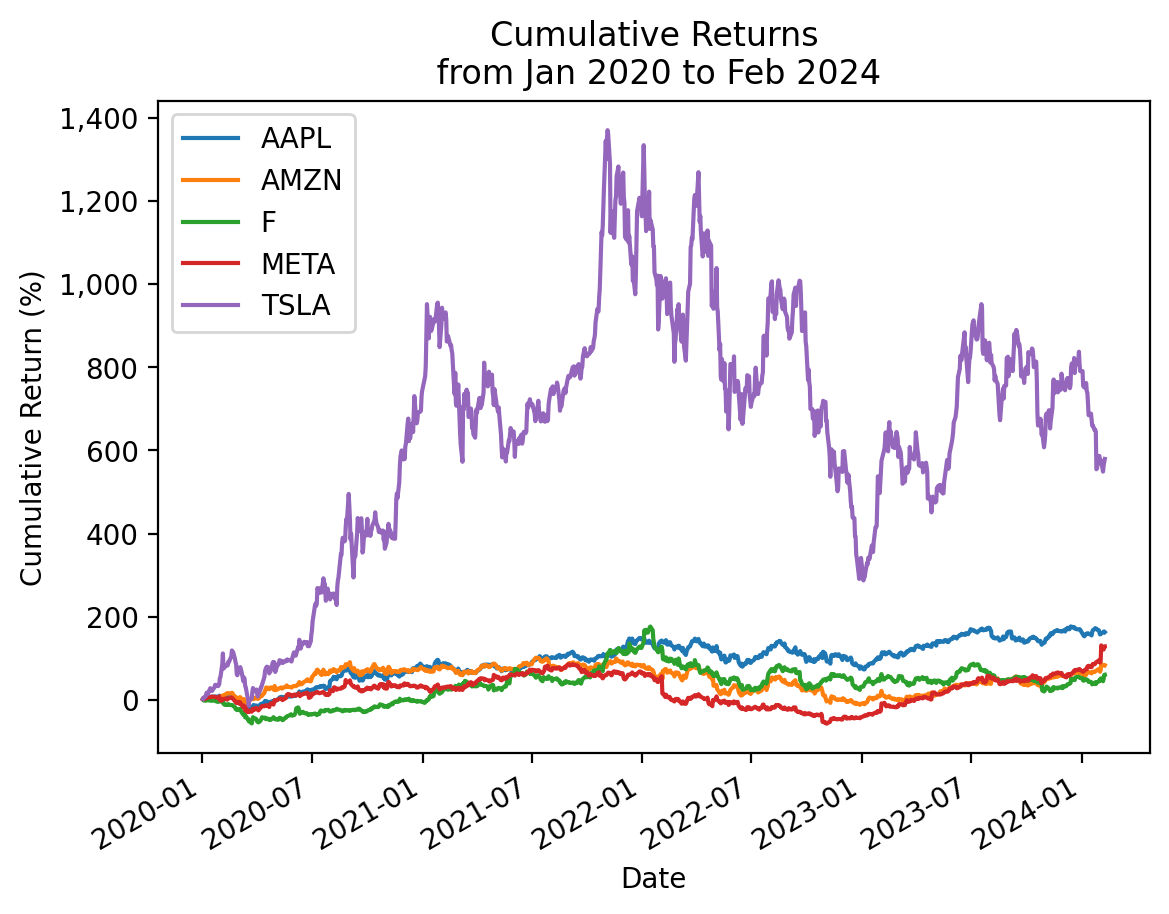
\includegraphics{herron_01_practice_05_files/figure-pdf/cell-15-output-1.png}

}

\end{figure}

\hypertarget{use-the-.cumsum-method-with-log-returns-to-plot-cumulative-returns-for-these-stocks-in-the-2020s-3}{%
\subsection{\texorpdfstring{Use the \texttt{.cumsum()} method with log
returns to plot cumulative returns for these stocks in the
2020s}{Use the .cumsum() method with log returns to plot cumulative returns for these stocks in the 2020s}}\label{use-the-.cumsum-method-with-log-returns-to-plot-cumulative-returns-for-these-stocks-in-the-2020s-3}}

\begin{Shaded}
\begin{Highlighting}[]
\NormalTok{cumret\_cumsum }\OperatorTok{=}\NormalTok{ (}
\NormalTok{    returns\_2020s }\CommentTok{\# returns during the 2020s}
\NormalTok{    .add(}\DecValTok{1}\NormalTok{) }\CommentTok{\# add 1 before we compound}
\NormalTok{    .pipe(np.log)}
\NormalTok{    .cumsum() }\CommentTok{\# log returns are additive!}
\NormalTok{    .pipe(np.exp)}
\NormalTok{    .sub(}\DecValTok{1}\NormalTok{) }\CommentTok{\# subtract 1 to recover cumulative return at time t}
\NormalTok{)}
\end{Highlighting}
\end{Shaded}

\begin{Shaded}
\begin{Highlighting}[]
\NormalTok{np.allclose(cumret\_cumprod, cumret\_cumsum)}
\end{Highlighting}
\end{Shaded}

\begin{verbatim}
True
\end{verbatim}

\begin{Shaded}
\begin{Highlighting}[]
\NormalTok{cumret\_cumsum.mul(}\DecValTok{100}\NormalTok{).plot()}

\CommentTok{\# https://stackoverflow.com/questions/25973581/how{-}to{-}format{-}axis{-}number{-}format{-}to{-}thousands{-}with{-}a{-}comma}
\ImportTok{from}\NormalTok{ matplotlib }\ImportTok{import}\NormalTok{ ticker}
\NormalTok{plt.gca().get\_yaxis().set\_major\_formatter(ticker.FuncFormatter(}\KeywordTok{lambda}\NormalTok{ x, p: }\BuiltInTok{format}\NormalTok{(}\BuiltInTok{int}\NormalTok{(x), }\StringTok{\textquotesingle{},\textquotesingle{}}\NormalTok{)))}

\NormalTok{plt.ylabel(}\StringTok{\textquotesingle{}Cumulative Return (\%)\textquotesingle{}}\NormalTok{)}
\NormalTok{plt.title(}\SpecialStringTok{f\textquotesingle{}Cumulative Returns}\CharTok{\textbackslash{}n}\SpecialStringTok{ from }\SpecialCharTok{\{}\NormalTok{returns\_2020s}\SpecialCharTok{.}\NormalTok{index}\SpecialCharTok{.}\BuiltInTok{min}\NormalTok{()}\SpecialCharTok{:}\OperatorTok{\%}\NormalTok{b }\OperatorTok{\%}\NormalTok{Y}\SpecialCharTok{\}}\SpecialStringTok{ to }\SpecialCharTok{\{}\NormalTok{returns\_2020s}\SpecialCharTok{.}\NormalTok{index}\SpecialCharTok{.}\BuiltInTok{max}\NormalTok{()}\SpecialCharTok{:}\OperatorTok{\%}\NormalTok{b }\OperatorTok{\%}\NormalTok{Y}\SpecialCharTok{\}}\SpecialStringTok{\textquotesingle{}}\NormalTok{)}
\NormalTok{plt.show()}
\end{Highlighting}
\end{Shaded}

\begin{figure}[H]

{\centering 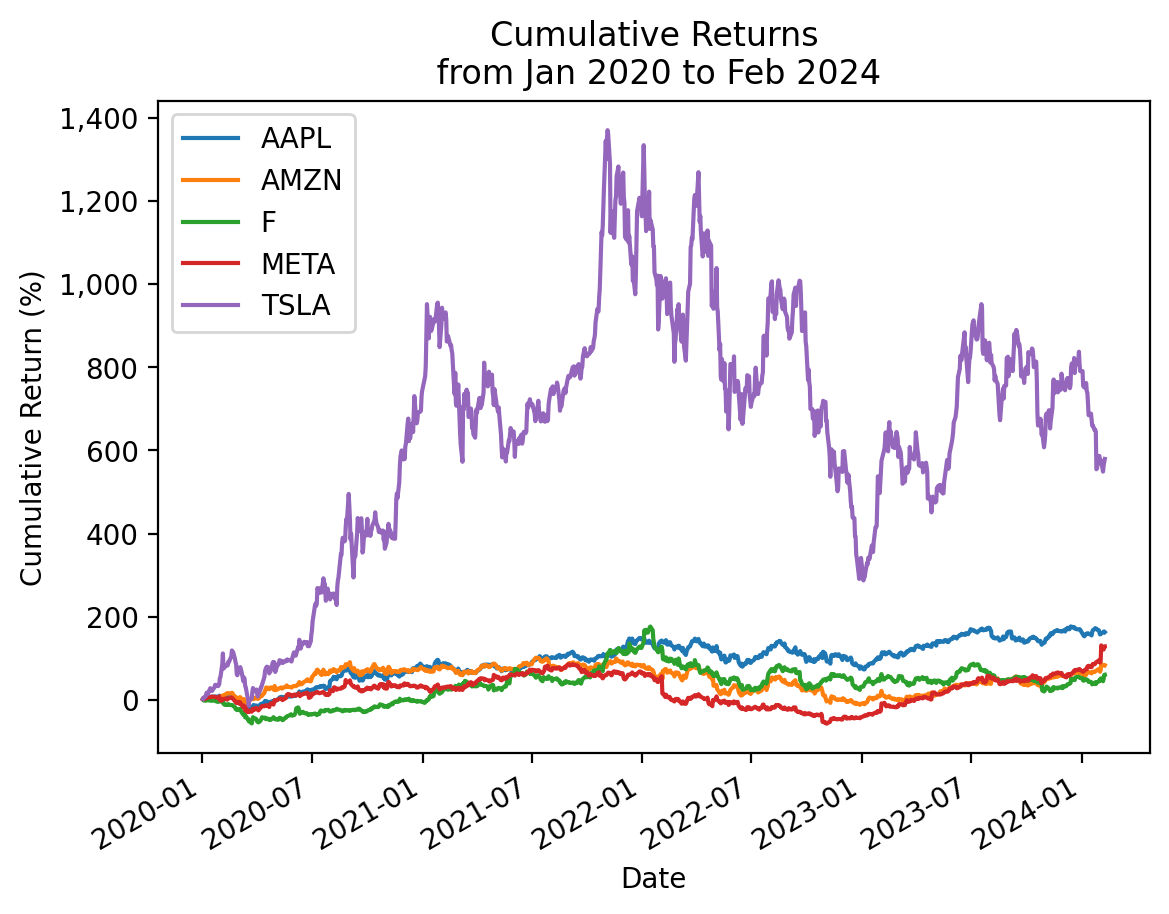
\includegraphics{herron_01_practice_05_files/figure-pdf/cell-18-output-1.png}

}

\end{figure}

\hypertarget{use-price-data-only-to-plot-cumulative-returns-for-these-stocks-in-the-2020s-3}{%
\subsection{Use price data only to plot cumulative returns for these
stocks in the
2020s}\label{use-price-data-only-to-plot-cumulative-returns-for-these-stocks-in-the-2020s-3}}

We can also calculate cumulative returns as the ratio of adjusted
closes. That is \(R_{0,T} = \frac{AC_T}{AC_0} - 1\). The trick here is
that \(FV_t = PV (1+r)^t\), so \((1+r)^t = \frac{FV_t}{PV}\).

\begin{Shaded}
\begin{Highlighting}[]
\NormalTok{returns\_2020s.iloc[}\DecValTok{0}\NormalTok{]}
\end{Highlighting}
\end{Shaded}

\begin{verbatim}
AAPL   0.0228
AMZN   0.0272
F      0.0129
META   0.0221
TSLA   0.0285
Name: 2020-01-02 00:00:00, dtype: float64
\end{verbatim}

\begin{Shaded}
\begin{Highlighting}[]
\NormalTok{prices[}\StringTok{\textquotesingle{}Adj Close\textquotesingle{}}\NormalTok{].loc[}\StringTok{\textquotesingle{}2020\textquotesingle{}}\NormalTok{].iloc[}\DecValTok{0}\NormalTok{]}
\end{Highlighting}
\end{Shaded}

\begin{verbatim}
AAPL    73.1526
AMZN    94.9005
F        8.0770
META   209.7800
TSLA    28.6840
Name: 2020-01-02 00:00:00, dtype: float64
\end{verbatim}

\begin{Shaded}
\begin{Highlighting}[]
\NormalTok{prices[}\StringTok{\textquotesingle{}Adj Close\textquotesingle{}}\NormalTok{].loc[}\StringTok{\textquotesingle{}2019\textquotesingle{}}\NormalTok{].iloc[}\OperatorTok{{-}}\DecValTok{1}\NormalTok{]}
\end{Highlighting}
\end{Shaded}

\begin{verbatim}
AAPL    71.5208
AMZN    92.3920
F        7.9741
META   205.2500
TSLA    27.8887
Name: 2019-12-31 00:00:00, dtype: float64
\end{verbatim}

\begin{Shaded}
\begin{Highlighting}[]
\NormalTok{prices[}\StringTok{\textquotesingle{}Adj Close\textquotesingle{}}\NormalTok{].loc[}\StringTok{\textquotesingle{}2020\textquotesingle{}}\NormalTok{].iloc[}\DecValTok{0}\NormalTok{] }\OperatorTok{/}\NormalTok{ prices[}\StringTok{\textquotesingle{}Adj Close\textquotesingle{}}\NormalTok{].loc[}\StringTok{\textquotesingle{}2019\textquotesingle{}}\NormalTok{].iloc[}\OperatorTok{{-}}\DecValTok{1}\NormalTok{] }\OperatorTok{{-}} \DecValTok{1}
\end{Highlighting}
\end{Shaded}

\begin{verbatim}
AAPL   0.0228
AMZN   0.0272
F      0.0129
META   0.0221
TSLA   0.0285
dtype: float64
\end{verbatim}

\textbf{\emph{Note:}} We drop the last row in
\texttt{prices{[}\textquotesingle{}Adj\ Close\textquotesingle{}{]}} with
\texttt{.iloc{[}:-1{]}}. We drop this last row here here because we did
the same above when we calculated \texttt{returns} to exclude possible
intraday returns.

\begin{Shaded}
\begin{Highlighting}[]
\NormalTok{cumret\_prices }\OperatorTok{=}\NormalTok{ prices[}\StringTok{\textquotesingle{}Adj Close\textquotesingle{}}\NormalTok{].loc[}\StringTok{\textquotesingle{}2020\textquotesingle{}}\NormalTok{:].iloc[:}\OperatorTok{{-}}\DecValTok{1}\NormalTok{] }\OperatorTok{/}\NormalTok{ prices[}\StringTok{\textquotesingle{}Adj Close\textquotesingle{}}\NormalTok{].loc[}\StringTok{\textquotesingle{}2019\textquotesingle{}}\NormalTok{].iloc[}\OperatorTok{{-}}\DecValTok{1}\NormalTok{] }\OperatorTok{{-}} \DecValTok{1}
\end{Highlighting}
\end{Shaded}

\begin{Shaded}
\begin{Highlighting}[]
\NormalTok{np.allclose(cumret\_prices, cumret\_cumprod)}
\end{Highlighting}
\end{Shaded}

\begin{verbatim}
True
\end{verbatim}

\begin{Shaded}
\begin{Highlighting}[]
\NormalTok{cumret\_prices.mul(}\DecValTok{100}\NormalTok{).plot()}

\CommentTok{\# https://stackoverflow.com/questions/25973581/how{-}to{-}format{-}axis{-}number{-}format{-}to{-}thousands{-}with{-}a{-}comma}
\ImportTok{from}\NormalTok{ matplotlib }\ImportTok{import}\NormalTok{ ticker}
\NormalTok{plt.gca().get\_yaxis().set\_major\_formatter(ticker.FuncFormatter(}\KeywordTok{lambda}\NormalTok{ x, p: }\BuiltInTok{format}\NormalTok{(}\BuiltInTok{int}\NormalTok{(x), }\StringTok{\textquotesingle{},\textquotesingle{}}\NormalTok{)))}

\NormalTok{plt.ylabel(}\StringTok{\textquotesingle{}Cumulative Return (\%)\textquotesingle{}}\NormalTok{)}
\NormalTok{plt.title(}\SpecialStringTok{f\textquotesingle{}Cumulative Returns}\CharTok{\textbackslash{}n}\SpecialStringTok{ from }\SpecialCharTok{\{}\NormalTok{returns\_2020s}\SpecialCharTok{.}\NormalTok{index}\SpecialCharTok{.}\BuiltInTok{min}\NormalTok{()}\SpecialCharTok{:}\OperatorTok{\%}\NormalTok{b }\OperatorTok{\%}\NormalTok{Y}\SpecialCharTok{\}}\SpecialStringTok{ to }\SpecialCharTok{\{}\NormalTok{returns\_2020s}\SpecialCharTok{.}\NormalTok{index}\SpecialCharTok{.}\BuiltInTok{max}\NormalTok{()}\SpecialCharTok{:}\OperatorTok{\%}\NormalTok{b }\OperatorTok{\%}\NormalTok{Y}\SpecialCharTok{\}}\SpecialStringTok{\textquotesingle{}}\NormalTok{)}
\NormalTok{plt.show()}
\end{Highlighting}
\end{Shaded}

\begin{figure}[H]

{\centering 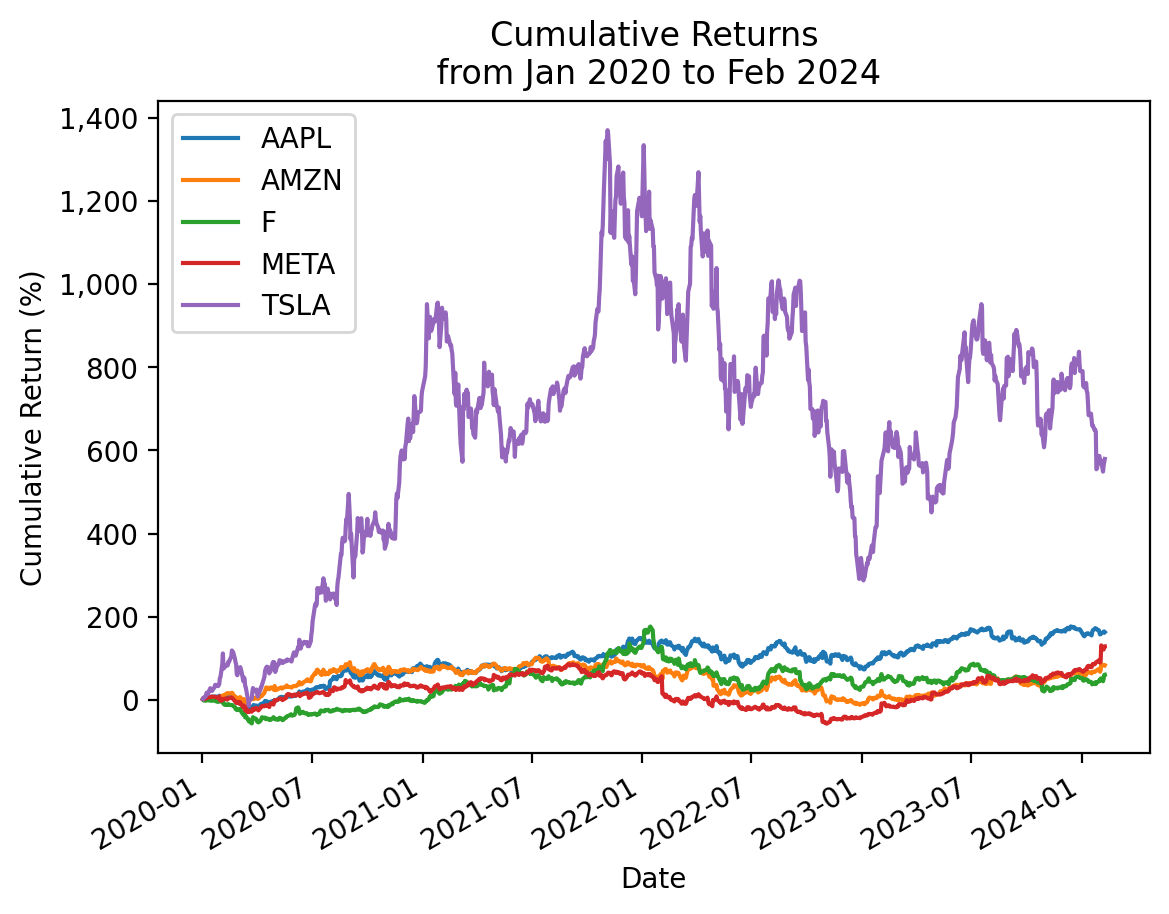
\includegraphics{herron_01_practice_05_files/figure-pdf/cell-25-output-1.png}

}

\end{figure}

\hypertarget{calculate-the-sharpe-ratio-for-tsla-3}{%
\subsection{Calculate the Sharpe Ratio for
TSLA}\label{calculate-the-sharpe-ratio-for-tsla-3}}

Calculate the Sharpe Ratio with all available returns and 2020s returns.
Recall the Sharpe Ratio is \(\frac{\overline{r_i - r_f}}{\sigma_i}\),
where \(\sigma_i\) is the volatility of \emph{excess} returns.

\textbf{\emph{I suggest you write a function named
\texttt{calc\_sharpe()} to use for the rest of this notebook.}}

\begin{Shaded}
\begin{Highlighting}[]
\KeywordTok{def}\NormalTok{ calc\_sharpe(ri, rf}\OperatorTok{=}\NormalTok{ff[}\StringTok{\textquotesingle{}RF\textquotesingle{}}\NormalTok{], ppy}\OperatorTok{=}\DecValTok{252}\NormalTok{):}
\NormalTok{    ri\_rf }\OperatorTok{=}\NormalTok{ ri.sub(rf).dropna()}
    \ControlFlowTok{return}\NormalTok{ np.sqrt(ppy) }\OperatorTok{*}\NormalTok{ ri\_rf.mean() }\OperatorTok{/}\NormalTok{ ri\_rf.std()}
\end{Highlighting}
\end{Shaded}

\begin{Shaded}
\begin{Highlighting}[]
\NormalTok{calc\_sharpe(ri}\OperatorTok{=}\NormalTok{returns[}\StringTok{\textquotesingle{}TSLA\textquotesingle{}}\NormalTok{])}
\end{Highlighting}
\end{Shaded}

\begin{verbatim}
0.9261
\end{verbatim}

\begin{Shaded}
\begin{Highlighting}[]
\NormalTok{calc\_sharpe(ri}\OperatorTok{=}\NormalTok{returns\_2020s[}\StringTok{\textquotesingle{}TSLA\textquotesingle{}}\NormalTok{])}
\end{Highlighting}
\end{Shaded}

\begin{verbatim}
1.1212
\end{verbatim}

We can use the \texttt{.pipe()} method here, too, since \texttt{ri} is
the first argument to \texttt{calc\_sharpe()}!

\begin{Shaded}
\begin{Highlighting}[]
\NormalTok{returns[}\StringTok{\textquotesingle{}TSLA\textquotesingle{}}\NormalTok{].pipe(calc\_sharpe)}
\end{Highlighting}
\end{Shaded}

\begin{verbatim}
0.9261
\end{verbatim}

\begin{Shaded}
\begin{Highlighting}[]
\NormalTok{returns\_2020s[}\StringTok{\textquotesingle{}TSLA\textquotesingle{}}\NormalTok{].pipe(calc\_sharpe)}
\end{Highlighting}
\end{Shaded}

\begin{verbatim}
1.1212
\end{verbatim}

\hypertarget{calculate-the-market-beta-for-tsla-3}{%
\subsection{Calculate the market beta for
TSLA}\label{calculate-the-market-beta-for-tsla-3}}

Calculate the market beta with all available returns and 2020s returns.
Recall we estimate market beta with the ordinary least squares (OLS)
regression \(R_i-R_f = \alpha + \beta (R_m-R_f) + \epsilon\). We can
estimate market beta with the covariance formula (i.e.,
\(\beta_i = \frac{Cov(R_i - R_f, R_m - R_f)}{Var(R_m-R_f)}\)) above for
a univariate regression if we do not need goodness of fit statistics.

\textbf{\emph{I suggest you write a function named \texttt{calc\_beta()}
to use for the rest of this notebook.}}

\begin{Shaded}
\begin{Highlighting}[]
\KeywordTok{def}\NormalTok{ calc\_beta(ri, rf}\OperatorTok{=}\NormalTok{ff[}\StringTok{\textquotesingle{}RF\textquotesingle{}}\NormalTok{], rm\_rf}\OperatorTok{=}\NormalTok{ff[}\StringTok{\textquotesingle{}Mkt{-}RF\textquotesingle{}}\NormalTok{]):}
\NormalTok{    ri\_rf }\OperatorTok{=}\NormalTok{ ri.sub(rf).dropna()}
    \ControlFlowTok{return}\NormalTok{ ri\_rf.cov(rm\_rf) }\OperatorTok{/}\NormalTok{ rm\_rf.loc[ri\_rf.index].var()}
\end{Highlighting}
\end{Shaded}

\begin{Shaded}
\begin{Highlighting}[]
\NormalTok{calc\_beta(ri}\OperatorTok{=}\NormalTok{returns[}\StringTok{\textquotesingle{}TSLA\textquotesingle{}}\NormalTok{])}
\end{Highlighting}
\end{Shaded}

\begin{verbatim}
1.4417
\end{verbatim}

\begin{Shaded}
\begin{Highlighting}[]
\NormalTok{calc\_beta(ri}\OperatorTok{=}\NormalTok{returns\_2020s[}\StringTok{\textquotesingle{}TSLA\textquotesingle{}}\NormalTok{])}
\end{Highlighting}
\end{Shaded}

\begin{verbatim}
1.5780
\end{verbatim}

We can use the \texttt{.pipe()} method here, too, since \texttt{ri} is
the first argument to \texttt{calc\_beta()}!

\begin{Shaded}
\begin{Highlighting}[]
\NormalTok{returns[}\StringTok{\textquotesingle{}TSLA\textquotesingle{}}\NormalTok{].pipe(calc\_beta)}
\end{Highlighting}
\end{Shaded}

\begin{verbatim}
1.4417
\end{verbatim}

\begin{Shaded}
\begin{Highlighting}[]
\NormalTok{returns\_2020s[}\StringTok{\textquotesingle{}TSLA\textquotesingle{}}\NormalTok{].pipe(calc\_beta)}
\end{Highlighting}
\end{Shaded}

\begin{verbatim}
1.5780
\end{verbatim}

\hypertarget{guess-the-sharpe-ratios-for-these-stocks-in-the-2020s-3}{%
\subsection{Guess the Sharpe Ratios for these stocks in the
2020s}\label{guess-the-sharpe-ratios-for-these-stocks-in-the-2020s-3}}

\hypertarget{guess-the-market-betas-for-these-stocks-in-the-2020s-3}{%
\subsection{Guess the market betas for these stocks in the
2020s}\label{guess-the-market-betas-for-these-stocks-in-the-2020s-3}}

\hypertarget{calculate-the-sharpe-ratios-for-these-stocks-in-the-2020s-3}{%
\subsection{Calculate the Sharpe Ratios for these stocks in the
2020s}\label{calculate-the-sharpe-ratios-for-these-stocks-in-the-2020s-3}}

How good were your guesses?

\begin{Shaded}
\begin{Highlighting}[]
\ControlFlowTok{for}\NormalTok{ i }\KeywordTok{in}\NormalTok{ returns\_2020s:}
\NormalTok{    sharpe\_i }\OperatorTok{=}\NormalTok{ returns\_2020s[i].pipe(calc\_sharpe)}
    \BuiltInTok{print}\NormalTok{(}\SpecialStringTok{f\textquotesingle{}Sharpe Ratio for }\SpecialCharTok{\{}\NormalTok{i}\SpecialCharTok{\}}\SpecialStringTok{:}\CharTok{\textbackslash{}t}\SpecialStringTok{ }\SpecialCharTok{\{}\NormalTok{sharpe\_i}\SpecialCharTok{:0.2f\}}\SpecialStringTok{\textquotesingle{}}\NormalTok{)}
\end{Highlighting}
\end{Shaded}

\begin{verbatim}
Sharpe Ratio for AAPL:   0.86
Sharpe Ratio for AMZN:   0.48
Sharpe Ratio for F:  0.42
Sharpe Ratio for META:   0.49
Sharpe Ratio for TSLA:   1.12
\end{verbatim}

We can also use pandas notation to vectorize this calculation. First
calculate \emph{excess} returns as \(r_i - r_f\).

\begin{Shaded}
\begin{Highlighting}[]
\NormalTok{returns\_2020s\_excess }\OperatorTok{=}\NormalTok{ returns\_2020s.sub(ff[}\StringTok{\textquotesingle{}RF\textquotesingle{}}\NormalTok{], axis}\OperatorTok{=}\DecValTok{0}\NormalTok{).dropna()}
\end{Highlighting}
\end{Shaded}

Then use pandas notation to calculate means, standard deviations, and
annualize.

\begin{Shaded}
\begin{Highlighting}[]
\NormalTok{(}
\NormalTok{    returns\_2020s\_excess}
\NormalTok{    .mean()}
\NormalTok{    .div(returns\_2020s\_excess.std())}
\NormalTok{    .mul(np.sqrt(}\DecValTok{252}\NormalTok{))}
\NormalTok{)}
\end{Highlighting}
\end{Shaded}

\begin{verbatim}
AAPL   0.8576
AMZN   0.4750
F      0.4240
META   0.4949
TSLA   1.1212
dtype: float64
\end{verbatim}

\textbf{\emph{Note:}} In a few weeks we will learn the \texttt{.apply()}
method, which avoids the loop syntax.

\begin{Shaded}
\begin{Highlighting}[]
\NormalTok{returns\_2020s.}\BuiltInTok{apply}\NormalTok{(calc\_sharpe)}
\end{Highlighting}
\end{Shaded}

\begin{verbatim}
AAPL   0.8576
AMZN   0.4750
F      0.4240
META   0.4949
TSLA   1.1212
dtype: float64
\end{verbatim}

\hypertarget{calculate-the-market-betas-for-these-stocks-in-the-2020s-3}{%
\subsection{Calculate the market betas for these stocks in the
2020s}\label{calculate-the-market-betas-for-these-stocks-in-the-2020s-3}}

How good were your guesses?

\begin{Shaded}
\begin{Highlighting}[]
\ControlFlowTok{for}\NormalTok{ i }\KeywordTok{in}\NormalTok{ returns\_2020s:}
\NormalTok{    beta\_i }\OperatorTok{=}\NormalTok{ returns\_2020s[i].pipe(calc\_beta)}
    \BuiltInTok{print}\NormalTok{(}\SpecialStringTok{f\textquotesingle{}Beta for }\SpecialCharTok{\{}\NormalTok{i}\SpecialCharTok{\}}\SpecialStringTok{:}\CharTok{\textbackslash{}t}\SpecialStringTok{ }\SpecialCharTok{\{}\NormalTok{beta\_i}\SpecialCharTok{:0.2f\}}\SpecialStringTok{\textquotesingle{}}\NormalTok{)}
\end{Highlighting}
\end{Shaded}

\begin{verbatim}
Beta for AAPL:   1.15
Beta for AMZN:   1.04
Beta for F:  1.22
Beta for META:   1.27
Beta for TSLA:   1.58
\end{verbatim}

Or we can follow out approach above to vectorize this calculation.
First, we need to add a market excess return column to
\texttt{returns\_2020s\_excess}.

\begin{Shaded}
\begin{Highlighting}[]
\NormalTok{returns\_2020s\_excess[}\StringTok{\textquotesingle{}Mkt{-}RF\textquotesingle{}}\NormalTok{] }\OperatorTok{=}\NormalTok{ ff[}\StringTok{\textquotesingle{}Mkt{-}RF\textquotesingle{}}\NormalTok{]}
\NormalTok{returns\_2020s\_excess.head()}
\end{Highlighting}
\end{Shaded}

\begin{longtable}[]{@{}lllllll@{}}
\toprule\noalign{}
& AAPL & AMZN & F & META & TSLA & Mkt-RF \\
Date & & & & & & \\
\midrule\noalign{}
\endhead
\bottomrule\noalign{}
\endlastfoot
2020-01-02 & 0.0228 & 0.0271 & 0.0128 & 0.0220 & 0.0285 & 0.0086 \\
2020-01-03 & -0.0098 & -0.0122 & -0.0224 & -0.0054 & 0.0296 & -0.0067 \\
2020-01-06 & 0.0079 & 0.0148 & -0.0055 & 0.0188 & 0.0192 & 0.0036 \\
2020-01-07 & -0.0048 & 0.0020 & 0.0098 & 0.0021 & 0.0387 & -0.0019 \\
2020-01-08 & 0.0160 & -0.0079 & -0.0001 & 0.0101 & 0.0491 & 0.0047 \\
\end{longtable}

\begin{Shaded}
\begin{Highlighting}[]
\NormalTok{vcv }\OperatorTok{=}\NormalTok{ returns\_2020s\_excess.cov()}
\NormalTok{vcv}
\end{Highlighting}
\end{Shaded}

\begin{longtable}[]{@{}lllllll@{}}
\toprule\noalign{}
& AAPL & AMZN & F & META & TSLA & Mkt-RF \\
\midrule\noalign{}
\endhead
\bottomrule\noalign{}
\endlastfoot
AAPL & 0.0004 & 0.0003 & 0.0002 & 0.0004 & 0.0005 & 0.0003 \\
AMZN & 0.0003 & 0.0006 & 0.0002 & 0.0004 & 0.0005 & 0.0002 \\
F & 0.0002 & 0.0002 & 0.0009 & 0.0003 & 0.0005 & 0.0003 \\
META & 0.0004 & 0.0004 & 0.0003 & 0.0009 & 0.0005 & 0.0003 \\
TSLA & 0.0005 & 0.0005 & 0.0005 & 0.0005 & 0.0018 & 0.0003 \\
Mkt-RF & 0.0003 & 0.0002 & 0.0003 & 0.0003 & 0.0003 & 0.0002 \\
\end{longtable}

\begin{Shaded}
\begin{Highlighting}[]
\NormalTok{vcv[}\StringTok{\textquotesingle{}Mkt{-}RF\textquotesingle{}}\NormalTok{].div(vcv.loc[}\StringTok{\textquotesingle{}Mkt{-}RF\textquotesingle{}}\NormalTok{, }\StringTok{\textquotesingle{}Mkt{-}RF\textquotesingle{}}\NormalTok{]).plot(kind}\OperatorTok{=}\StringTok{\textquotesingle{}bar\textquotesingle{}}\NormalTok{)}
\NormalTok{plt.xlabel(}\StringTok{\textquotesingle{}Ticker\textquotesingle{}}\NormalTok{)}
\NormalTok{plt.ylabel(}\StringTok{\textquotesingle{}CAPM Beta\textquotesingle{}}\NormalTok{)}
\NormalTok{plt.title(}\StringTok{\textquotesingle{}CAPM Betas\textquotesingle{}}\NormalTok{)}
\NormalTok{plt.show()}
\end{Highlighting}
\end{Shaded}

\begin{figure}[H]

{\centering 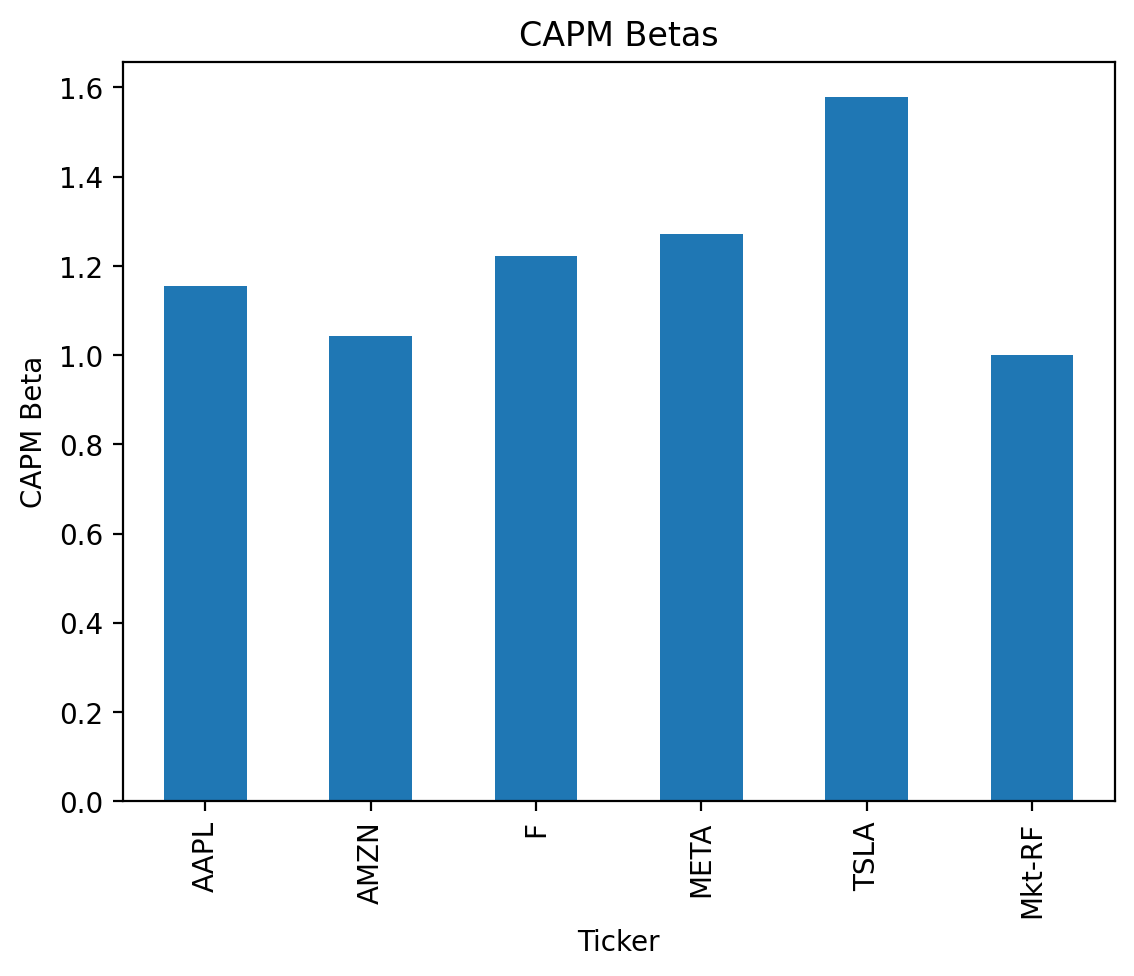
\includegraphics{herron_01_practice_05_files/figure-pdf/cell-43-output-1.png}

}

\end{figure}

\textbf{\emph{Note:}} In a few weeks we will learn the \texttt{.apply()}
method, which avoids the loop syntax.

\begin{Shaded}
\begin{Highlighting}[]
\NormalTok{returns\_2020s.}\BuiltInTok{apply}\NormalTok{(calc\_beta)}
\end{Highlighting}
\end{Shaded}

\begin{verbatim}
AAPL   1.1541
AMZN   1.0429
F      1.2231
META   1.2710
TSLA   1.5780
dtype: float64
\end{verbatim}

\hypertarget{calculate-the-sharpe-ratio-for-an-equally-weighted-portfolio-of-these-stocks-in-the-2020s-3}{%
\subsection{\texorpdfstring{Calculate the Sharpe Ratio for an
\emph{equally weighted} portfolio of these stocks in the
2020s}{Calculate the Sharpe Ratio for an equally weighted portfolio of these stocks in the 2020s}}\label{calculate-the-sharpe-ratio-for-an-equally-weighted-portfolio-of-these-stocks-in-the-2020s-3}}

What do you notice?

\begin{Shaded}
\begin{Highlighting}[]
\NormalTok{returns\_2020s.mean(axis}\OperatorTok{=}\DecValTok{1}\NormalTok{).pipe(calc\_sharpe)}
\end{Highlighting}
\end{Shaded}

\begin{verbatim}
0.9573
\end{verbatim}

Because diversification reduces portfolio standard deviation less than
the sum of its parts, the Sharpe Ratio of the equally weighted portfolio
is less than the equally weighted mean of the single-stock Sharpe
Ratios.

\begin{Shaded}
\begin{Highlighting}[]
\NormalTok{returns\_2020s.}\BuiltInTok{apply}\NormalTok{(calc\_sharpe).mean()}
\end{Highlighting}
\end{Shaded}

\begin{verbatim}
0.6745
\end{verbatim}

\hypertarget{calculate-the-market-beta-for-an-equally-weighted-portfolio-of-these-stocks-in-the-2020s-3}{%
\subsection{\texorpdfstring{Calculate the market beta for an
\emph{equally weighted} portfolio of these stocks in the
2020s}{Calculate the market beta for an equally weighted portfolio of these stocks in the 2020s}}\label{calculate-the-market-beta-for-an-equally-weighted-portfolio-of-these-stocks-in-the-2020s-3}}

What do you notice?

Beta measures \emph{non}diversifiable risk, so
\(\beta_P = \sum w_i \beta_i\)!

\begin{Shaded}
\begin{Highlighting}[]
\NormalTok{returns\_2020s.mean(axis}\OperatorTok{=}\DecValTok{1}\NormalTok{).pipe(calc\_beta)}
\end{Highlighting}
\end{Shaded}

\begin{verbatim}
1.2538
\end{verbatim}

\begin{Shaded}
\begin{Highlighting}[]
\NormalTok{returns\_2020s.}\BuiltInTok{apply}\NormalTok{(calc\_beta).mean()}
\end{Highlighting}
\end{Shaded}

\begin{verbatim}
1.2538
\end{verbatim}

\hypertarget{calculate-the-market-betas-for-these-stocks-every-calendar-year-for-every-possible-year-3}{%
\subsection{Calculate the market betas for these stocks every calendar
year for every possible
year}\label{calculate-the-market-betas-for-these-stocks-every-calendar-year-for-every-possible-year-3}}

Save these market betas to data frame \texttt{betas}. Our current Python
knowledge limits us to a for-loop, but we will learn easier and faster
approaches soon!

\begin{Shaded}
\begin{Highlighting}[]
\NormalTok{betas }\OperatorTok{=}\NormalTok{ pd.DataFrame(}
\NormalTok{    index}\OperatorTok{=}\BuiltInTok{range}\NormalTok{(}\DecValTok{1972}\NormalTok{, }\DecValTok{2024}\NormalTok{),}
\NormalTok{    columns}\OperatorTok{=}\NormalTok{returns.columns}
\NormalTok{)}

\NormalTok{betas.columns.name }\OperatorTok{=} \StringTok{\textquotesingle{}Ticker\textquotesingle{}}
\NormalTok{betas.index.name }\OperatorTok{=} \StringTok{\textquotesingle{}Year\textquotesingle{}}

\NormalTok{betas.tail()}
\end{Highlighting}
\end{Shaded}

\begin{longtable}[]{@{}llllll@{}}
\toprule\noalign{}
Ticker & AAPL & AMZN & F & META & TSLA \\
Year & & & & & \\
\midrule\noalign{}
\endhead
\bottomrule\noalign{}
\endlastfoot
2019 & NaN & NaN & NaN & NaN & NaN \\
2020 & NaN & NaN & NaN & NaN & NaN \\
2021 & NaN & NaN & NaN & NaN & NaN \\
2022 & NaN & NaN & NaN & NaN & NaN \\
2023 & NaN & NaN & NaN & NaN & NaN \\
\end{longtable}

\begin{Shaded}
\begin{Highlighting}[]
\ControlFlowTok{for}\NormalTok{ i }\KeywordTok{in}\NormalTok{ betas.index: }
    \ControlFlowTok{for}\NormalTok{ c }\KeywordTok{in}\NormalTok{ betas.columns:}
\NormalTok{        betas.at[i, c] }\OperatorTok{=}\NormalTok{ returns.loc[}\BuiltInTok{str}\NormalTok{(i), c].pipe(calc\_beta)}

\NormalTok{betas.tail()}
\end{Highlighting}
\end{Shaded}

\begin{longtable}[]{@{}llllll@{}}
\toprule\noalign{}
Ticker & AAPL & AMZN & F & META & TSLA \\
Year & & & & & \\
\midrule\noalign{}
\endhead
\bottomrule\noalign{}
\endlastfoot
2019 & 1.4751 & 1.2752 & 1.0733 & 1.2094 & 1.3262 \\
2020 & 1.1174 & 0.6866 & 1.1052 & 0.9913 & 1.3041 \\
2021 & 1.1957 & 0.9822 & 1.2396 & 1.2014 & 1.9891 \\
2022 & 1.2386 & 1.5922 & 1.3824 & 1.6843 & 1.7414 \\
2023 & 1.0369 & 1.4649 & 1.3947 & 1.6630 & 2.2218 \\
\end{longtable}

\hypertarget{plot-the-time-series-of-market-betas-3}{%
\subsection{Plot the time series of market
betas}\label{plot-the-time-series-of-market-betas-3}}

\begin{Shaded}
\begin{Highlighting}[]
\NormalTok{betas.plot()}
\NormalTok{plt.ylabel(}\StringTok{\textquotesingle{}CAPM Beta\textquotesingle{}}\NormalTok{)}
\NormalTok{plt.title(}\StringTok{\textquotesingle{}CAPM Betas\textquotesingle{}}\NormalTok{)}
\NormalTok{plt.show()}
\end{Highlighting}
\end{Shaded}

\begin{figure}[H]

{\centering 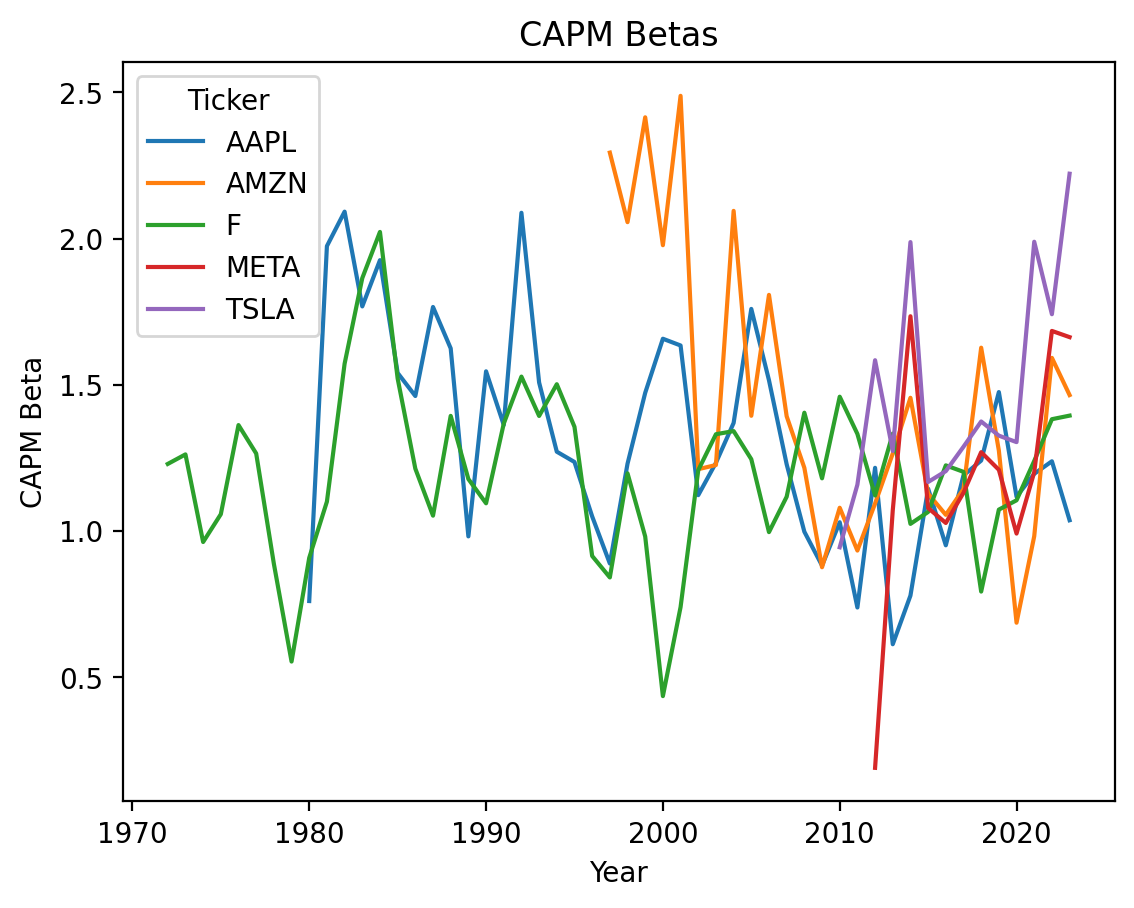
\includegraphics{herron_01_practice_05_files/figure-pdf/cell-51-output-1.png}

}

\end{figure}

\part{Week 6}

\hypertarget{mckinney-chapter-8---data-wrangling-join-combine-and-reshape}{%
\chapter{McKinney Chapter 8 - Data Wrangling: Join, Combine, and
Reshape}\label{mckinney-chapter-8---data-wrangling-join-combine-and-reshape}}

\hypertarget{introduction-4}{%
\section{Introduction}\label{introduction-4}}

Chapter 8 of Wes McKinney's
\href{https://wesmckinney.com/book/}{\emph{Python for Data Analysis}}
introduces a few important pandas concepts:

\begin{enumerate}
\def\labelenumi{\arabic{enumi}.}
\tightlist
\item
  Joining or merging is combining 2+ data frames on 1+ indexes or
  columns into 1 data frame
\item
  Reshaping is rearranging data frames so it has fewer columns and more
  rows (wide to long) or more columns and fewer rows (long to wide); we
  can also reshape a series to a data frame and vice versa
\end{enumerate}

\textbf{\emph{Note:}} Indented block quotes are from McKinney unless
otherwise indicated. The section numbers here differ from McKinney
because we will only discuss some topics.

\begin{Shaded}
\begin{Highlighting}[]
\ImportTok{import}\NormalTok{ matplotlib.pyplot }\ImportTok{as}\NormalTok{ plt}
\ImportTok{import}\NormalTok{ numpy }\ImportTok{as}\NormalTok{ np}
\ImportTok{import}\NormalTok{ pandas }\ImportTok{as}\NormalTok{ pd}
\ImportTok{import}\NormalTok{ pandas\_datareader }\ImportTok{as}\NormalTok{ pdr}
\ImportTok{import}\NormalTok{ yfinance }\ImportTok{as}\NormalTok{ yf}
\end{Highlighting}
\end{Shaded}

\begin{Shaded}
\begin{Highlighting}[]
\OperatorTok{\%}\NormalTok{precision }\DecValTok{4}
\NormalTok{pd.options.display.float\_format }\OperatorTok{=} \StringTok{\textquotesingle{}}\SpecialCharTok{\{:.4f\}}\StringTok{\textquotesingle{}}\NormalTok{.}\BuiltInTok{format}
\OperatorTok{\%}\NormalTok{config InlineBackend.figure\_format }\OperatorTok{=} \StringTok{\textquotesingle{}retina\textquotesingle{}}
\end{Highlighting}
\end{Shaded}

\hypertarget{hierarchical-indexing}{%
\section{Hierarchical Indexing}\label{hierarchical-indexing}}

We need to learn about hierarchical indexing before we learn about
combining and reshaping data. A hierarchical index gives two or more
index levels to an axis. For example, we could index rows by ticker and
date. Or we could index columns by variable and ticker. Hierarchical
indexing helps us work with high-dimensional data in a low-dimensional
form.

\begin{Shaded}
\begin{Highlighting}[]
\NormalTok{np.random.seed(}\DecValTok{42}\NormalTok{)}
\NormalTok{data }\OperatorTok{=}\NormalTok{ pd.Series(}
\NormalTok{    data}\OperatorTok{=}\NormalTok{np.random.randn(}\DecValTok{9}\NormalTok{),}
\NormalTok{    index}\OperatorTok{=}\NormalTok{[}
\NormalTok{        [}\StringTok{\textquotesingle{}a\textquotesingle{}}\NormalTok{, }\StringTok{\textquotesingle{}a\textquotesingle{}}\NormalTok{, }\StringTok{\textquotesingle{}a\textquotesingle{}}\NormalTok{, }\StringTok{\textquotesingle{}b\textquotesingle{}}\NormalTok{, }\StringTok{\textquotesingle{}b\textquotesingle{}}\NormalTok{, }\StringTok{\textquotesingle{}c\textquotesingle{}}\NormalTok{, }\StringTok{\textquotesingle{}c\textquotesingle{}}\NormalTok{, }\StringTok{\textquotesingle{}d\textquotesingle{}}\NormalTok{, }\StringTok{\textquotesingle{}d\textquotesingle{}}\NormalTok{],}
\NormalTok{        [}\DecValTok{1}\NormalTok{, }\DecValTok{2}\NormalTok{, }\DecValTok{3}\NormalTok{, }\DecValTok{1}\NormalTok{, }\DecValTok{3}\NormalTok{, }\DecValTok{1}\NormalTok{, }\DecValTok{2}\NormalTok{, }\DecValTok{2}\NormalTok{, }\DecValTok{3}\NormalTok{]}
\NormalTok{    ]}
\NormalTok{)}

\NormalTok{data}
\end{Highlighting}
\end{Shaded}

\begin{verbatim}
a  1    0.4967
   2   -0.1383
   3    0.6477
b  1    1.5230
   3   -0.2342
c  1   -0.2341
   2    1.5792
d  2    0.7674
   3   -0.4695
dtype: float64
\end{verbatim}

We can partially index this series to concisely subset data.

\begin{Shaded}
\begin{Highlighting}[]
\NormalTok{data[}\StringTok{\textquotesingle{}b\textquotesingle{}}\NormalTok{]}
\end{Highlighting}
\end{Shaded}

\begin{verbatim}
1    1.5230
3   -0.2342
dtype: float64
\end{verbatim}

\begin{Shaded}
\begin{Highlighting}[]
\NormalTok{data[}\StringTok{\textquotesingle{}b\textquotesingle{}}\NormalTok{:}\StringTok{\textquotesingle{}c\textquotesingle{}}\NormalTok{]}
\end{Highlighting}
\end{Shaded}

\begin{verbatim}
b  1    1.5230
   3   -0.2342
c  1   -0.2341
   2    1.5792
dtype: float64
\end{verbatim}

\begin{Shaded}
\begin{Highlighting}[]
\NormalTok{data.loc[[}\StringTok{\textquotesingle{}b\textquotesingle{}}\NormalTok{, }\StringTok{\textquotesingle{}d\textquotesingle{}}\NormalTok{]]}
\end{Highlighting}
\end{Shaded}

\begin{verbatim}
b  1    1.5230
   3   -0.2342
d  2    0.7674
   3   -0.4695
dtype: float64
\end{verbatim}

We can subset on the index inner level, too. Here the first \texttt{:}
slices all values in the outer index.

\begin{Shaded}
\begin{Highlighting}[]
\NormalTok{data.loc[:, }\DecValTok{2}\NormalTok{]}
\end{Highlighting}
\end{Shaded}

\begin{verbatim}
a   -0.1383
c    1.5792
d    0.7674
dtype: float64
\end{verbatim}

Here \texttt{data} has a stacked format. For each outer index level (the
letters), we have multiple observations based on the inner index level
(the numbers). We can un-stack \texttt{data} to convert the inner index
level to columns.

\begin{Shaded}
\begin{Highlighting}[]
\NormalTok{data.unstack()}
\end{Highlighting}
\end{Shaded}

\begin{longtable}[]{@{}llll@{}}
\toprule\noalign{}
& 1 & 2 & 3 \\
\midrule\noalign{}
\endhead
\bottomrule\noalign{}
\endlastfoot
a & 0.4967 & -0.1383 & 0.6477 \\
b & 1.5230 & NaN & -0.2342 \\
c & -0.2341 & 1.5792 & NaN \\
d & NaN & 0.7674 & -0.4695 \\
\end{longtable}

\begin{Shaded}
\begin{Highlighting}[]
\NormalTok{data.unstack().stack()}
\end{Highlighting}
\end{Shaded}

\begin{verbatim}
a  1    0.4967
   2   -0.1383
   3    0.6477
b  1    1.5230
   3   -0.2342
c  1   -0.2341
   2    1.5792
d  2    0.7674
   3   -0.4695
dtype: float64
\end{verbatim}

We can create a data frame with hieracrhical indexes or multi-indexes on
rows \emph{and} columns.

\begin{Shaded}
\begin{Highlighting}[]
\NormalTok{frame }\OperatorTok{=}\NormalTok{ pd.DataFrame(}
\NormalTok{    data}\OperatorTok{=}\NormalTok{np.arange(}\DecValTok{12}\NormalTok{).reshape((}\DecValTok{4}\NormalTok{, }\DecValTok{3}\NormalTok{)),}
\NormalTok{    index}\OperatorTok{=}\NormalTok{[[}\StringTok{\textquotesingle{}a\textquotesingle{}}\NormalTok{, }\StringTok{\textquotesingle{}a\textquotesingle{}}\NormalTok{, }\StringTok{\textquotesingle{}b\textquotesingle{}}\NormalTok{, }\StringTok{\textquotesingle{}b\textquotesingle{}}\NormalTok{], [}\DecValTok{1}\NormalTok{, }\DecValTok{2}\NormalTok{, }\DecValTok{1}\NormalTok{, }\DecValTok{2}\NormalTok{]],}
\NormalTok{    columns}\OperatorTok{=}\NormalTok{[[}\StringTok{\textquotesingle{}Ohio\textquotesingle{}}\NormalTok{, }\StringTok{\textquotesingle{}Ohio\textquotesingle{}}\NormalTok{, }\StringTok{\textquotesingle{}Colorado\textquotesingle{}}\NormalTok{], [}\StringTok{\textquotesingle{}Green\textquotesingle{}}\NormalTok{, }\StringTok{\textquotesingle{}Red\textquotesingle{}}\NormalTok{, }\StringTok{\textquotesingle{}Green\textquotesingle{}}\NormalTok{]]}
\NormalTok{)}

\NormalTok{frame}
\end{Highlighting}
\end{Shaded}

\begin{longtable}[]{@{}lllll@{}}
\toprule\noalign{}
& &
\multicolumn{2}{>{\raggedright\arraybackslash}p{(\columnwidth - 8\tabcolsep) * \real{0.0000} + 2\tabcolsep}}{%
Ohio} & Colorado \\
& & Green & Red & Green \\
\midrule\noalign{}
\endhead
\bottomrule\noalign{}
\endlastfoot
\multirow{2}{*}{a} & 1 & 0 & 1 & 2 \\
& 2 & 3 & 4 & 5 \\
\multirow{2}{*}{b} & 1 & 6 & 7 & 8 \\
& 2 & 9 & 10 & 11 \\
\end{longtable}

We can name these multi-indexes but names are not required.

\begin{Shaded}
\begin{Highlighting}[]
\NormalTok{frame.index.names }\OperatorTok{=}\NormalTok{ [}\StringTok{\textquotesingle{}key1\textquotesingle{}}\NormalTok{, }\StringTok{\textquotesingle{}key2\textquotesingle{}}\NormalTok{]}
\NormalTok{frame.columns.names }\OperatorTok{=}\NormalTok{ [}\StringTok{\textquotesingle{}state\textquotesingle{}}\NormalTok{, }\StringTok{\textquotesingle{}color\textquotesingle{}}\NormalTok{]}
\NormalTok{frame}
\end{Highlighting}
\end{Shaded}

\begin{longtable}[]{@{}lllll@{}}
\toprule\noalign{}
& state &
\multicolumn{2}{>{\raggedright\arraybackslash}p{(\columnwidth - 8\tabcolsep) * \real{0.0000} + 2\tabcolsep}}{%
Ohio} & Colorado \\
& color & Green & Red & Green \\
key1 & key2 & & & \\
\midrule\noalign{}
\endhead
\bottomrule\noalign{}
\endlastfoot
\multirow{2}{*}{a} & 1 & 0 & 1 & 2 \\
& 2 & 3 & 4 & 5 \\
\multirow{2}{*}{b} & 1 & 6 & 7 & 8 \\
& 2 & 9 & 10 & 11 \\
\end{longtable}

Recall that \texttt{df{[}val{]}} selects the \texttt{val} column. Here
\texttt{frame} has a multi-index for the columns, so
\texttt{frame{[}\textquotesingle{}Ohio\textquotesingle{}{]}} selects all
columns with Ohio as the outer index level.

\begin{Shaded}
\begin{Highlighting}[]
\NormalTok{frame[}\StringTok{\textquotesingle{}Ohio\textquotesingle{}}\NormalTok{]}
\end{Highlighting}
\end{Shaded}

\begin{longtable}[]{@{}llll@{}}
\toprule\noalign{}
& color & Green & Red \\
key1 & key2 & & \\
\midrule\noalign{}
\endhead
\bottomrule\noalign{}
\endlastfoot
\multirow{2}{*}{a} & 1 & 0 & 1 \\
& 2 & 3 & 4 \\
\multirow{2}{*}{b} & 1 & 6 & 7 \\
& 2 & 9 & 10 \\
\end{longtable}

We can pass a tuple if we only want one column.

\begin{Shaded}
\begin{Highlighting}[]
\NormalTok{frame[[(}\StringTok{\textquotesingle{}Ohio\textquotesingle{}}\NormalTok{, }\StringTok{\textquotesingle{}Green\textquotesingle{}}\NormalTok{)]]}
\end{Highlighting}
\end{Shaded}

\begin{longtable}[]{@{}lll@{}}
\toprule\noalign{}
& state & Ohio \\
& color & Green \\
key1 & key2 & \\
\midrule\noalign{}
\endhead
\bottomrule\noalign{}
\endlastfoot
\multirow{2}{*}{a} & 1 & 0 \\
& 2 & 3 \\
\multirow{2}{*}{b} & 1 & 6 \\
& 2 & 9 \\
\end{longtable}

We have to do a more work to slice the inner level of the column index.

\begin{Shaded}
\begin{Highlighting}[]
\NormalTok{frame.loc[:, (}\BuiltInTok{slice}\NormalTok{(}\VariableTok{None}\NormalTok{), }\StringTok{\textquotesingle{}Green\textquotesingle{}}\NormalTok{)]}
\end{Highlighting}
\end{Shaded}

\begin{longtable}[]{@{}llll@{}}
\toprule\noalign{}
& state & Ohio & Colorado \\
& color & Green & Green \\
key1 & key2 & & \\
\midrule\noalign{}
\endhead
\bottomrule\noalign{}
\endlastfoot
\multirow{2}{*}{a} & 1 & 0 & 2 \\
& 2 & 3 & 5 \\
\multirow{2}{*}{b} & 1 & 6 & 8 \\
& 2 & 9 & 11 \\
\end{longtable}

We can use
\texttt{pd.IndexSlice{[}:,\ \textquotesingle{}Green\textquotesingle{}{]}}
an alternative to
\texttt{(slice(None),\ \textquotesingle{}Green\textquotesingle{})}.

\begin{Shaded}
\begin{Highlighting}[]
\NormalTok{frame.loc[:, pd.IndexSlice[:, }\StringTok{\textquotesingle{}Green\textquotesingle{}}\NormalTok{]]}
\end{Highlighting}
\end{Shaded}

\begin{longtable}[]{@{}llll@{}}
\toprule\noalign{}
& state & Ohio & Colorado \\
& color & Green & Green \\
key1 & key2 & & \\
\midrule\noalign{}
\endhead
\bottomrule\noalign{}
\endlastfoot
\multirow{2}{*}{a} & 1 & 0 & 2 \\
& 2 & 3 & 5 \\
\multirow{2}{*}{b} & 1 & 6 & 8 \\
& 2 & 9 & 11 \\
\end{longtable}

\hypertarget{reordering-and-sorting-levels}{%
\subsection{Reordering and Sorting
Levels}\label{reordering-and-sorting-levels}}

We can swap index levels with the \texttt{.swaplevel()} method. The
default arguments are \texttt{i=-2} and \texttt{j=-1}, which swap the
two innermost index levels.

\begin{Shaded}
\begin{Highlighting}[]
\NormalTok{frame}
\end{Highlighting}
\end{Shaded}

\begin{longtable}[]{@{}lllll@{}}
\toprule\noalign{}
& state &
\multicolumn{2}{>{\raggedright\arraybackslash}p{(\columnwidth - 8\tabcolsep) * \real{0.0000} + 2\tabcolsep}}{%
Ohio} & Colorado \\
& color & Green & Red & Green \\
key1 & key2 & & & \\
\midrule\noalign{}
\endhead
\bottomrule\noalign{}
\endlastfoot
\multirow{2}{*}{a} & 1 & 0 & 1 & 2 \\
& 2 & 3 & 4 & 5 \\
\multirow{2}{*}{b} & 1 & 6 & 7 & 8 \\
& 2 & 9 & 10 & 11 \\
\end{longtable}

\begin{Shaded}
\begin{Highlighting}[]
\NormalTok{frame.swaplevel()}
\end{Highlighting}
\end{Shaded}

\begin{longtable}[]{@{}lllll@{}}
\toprule\noalign{}
& state &
\multicolumn{2}{>{\raggedright\arraybackslash}p{(\columnwidth - 8\tabcolsep) * \real{0.0000} + 2\tabcolsep}}{%
Ohio} & Colorado \\
& color & Green & Red & Green \\
key2 & key1 & & & \\
\midrule\noalign{}
\endhead
\bottomrule\noalign{}
\endlastfoot
1 & a & 0 & 1 & 2 \\
2 & a & 3 & 4 & 5 \\
1 & b & 6 & 7 & 8 \\
2 & b & 9 & 10 & 11 \\
\end{longtable}

We can use index \emph{names}, too.

\begin{Shaded}
\begin{Highlighting}[]
\NormalTok{frame.swaplevel(}\StringTok{\textquotesingle{}key1\textquotesingle{}}\NormalTok{, }\StringTok{\textquotesingle{}key2\textquotesingle{}}\NormalTok{)}
\end{Highlighting}
\end{Shaded}

\begin{longtable}[]{@{}lllll@{}}
\toprule\noalign{}
& state &
\multicolumn{2}{>{\raggedright\arraybackslash}p{(\columnwidth - 8\tabcolsep) * \real{0.0000} + 2\tabcolsep}}{%
Ohio} & Colorado \\
& color & Green & Red & Green \\
key2 & key1 & & & \\
\midrule\noalign{}
\endhead
\bottomrule\noalign{}
\endlastfoot
1 & a & 0 & 1 & 2 \\
2 & a & 3 & 4 & 5 \\
1 & b & 6 & 7 & 8 \\
2 & b & 9 & 10 & 11 \\
\end{longtable}

We can also sort on an index (or list of indexes). After we swap levels,
we may want to sort our data.

\begin{Shaded}
\begin{Highlighting}[]
\NormalTok{frame}
\end{Highlighting}
\end{Shaded}

\begin{longtable}[]{@{}lllll@{}}
\toprule\noalign{}
& state &
\multicolumn{2}{>{\raggedright\arraybackslash}p{(\columnwidth - 8\tabcolsep) * \real{0.0000} + 2\tabcolsep}}{%
Ohio} & Colorado \\
& color & Green & Red & Green \\
key1 & key2 & & & \\
\midrule\noalign{}
\endhead
\bottomrule\noalign{}
\endlastfoot
\multirow{2}{*}{a} & 1 & 0 & 1 & 2 \\
& 2 & 3 & 4 & 5 \\
\multirow{2}{*}{b} & 1 & 6 & 7 & 8 \\
& 2 & 9 & 10 & 11 \\
\end{longtable}

\begin{Shaded}
\begin{Highlighting}[]
\NormalTok{frame.sort\_index(level}\OperatorTok{=}\DecValTok{1}\NormalTok{)}
\end{Highlighting}
\end{Shaded}

\begin{longtable}[]{@{}lllll@{}}
\toprule\noalign{}
& state &
\multicolumn{2}{>{\raggedright\arraybackslash}p{(\columnwidth - 8\tabcolsep) * \real{0.0000} + 2\tabcolsep}}{%
Ohio} & Colorado \\
& color & Green & Red & Green \\
key1 & key2 & & & \\
\midrule\noalign{}
\endhead
\bottomrule\noalign{}
\endlastfoot
a & 1 & 0 & 1 & 2 \\
b & 1 & 6 & 7 & 8 \\
a & 2 & 3 & 4 & 5 \\
b & 2 & 9 & 10 & 11 \\
\end{longtable}

Again, we can give index \emph{names}, too.

\begin{Shaded}
\begin{Highlighting}[]
\NormalTok{frame.sort\_index(level}\OperatorTok{=}\StringTok{\textquotesingle{}key2\textquotesingle{}}\NormalTok{)}
\end{Highlighting}
\end{Shaded}

\begin{longtable}[]{@{}lllll@{}}
\toprule\noalign{}
& state &
\multicolumn{2}{>{\raggedright\arraybackslash}p{(\columnwidth - 8\tabcolsep) * \real{0.0000} + 2\tabcolsep}}{%
Ohio} & Colorado \\
& color & Green & Red & Green \\
key1 & key2 & & & \\
\midrule\noalign{}
\endhead
\bottomrule\noalign{}
\endlastfoot
a & 1 & 0 & 1 & 2 \\
b & 1 & 6 & 7 & 8 \\
a & 2 & 3 & 4 & 5 \\
b & 2 & 9 & 10 & 11 \\
\end{longtable}

We can sort by two or more index levels by passing a list of index
levels or names.

\begin{Shaded}
\begin{Highlighting}[]
\NormalTok{frame.sort\_index(level}\OperatorTok{=}\NormalTok{[}\DecValTok{0}\NormalTok{, }\DecValTok{1}\NormalTok{])}
\end{Highlighting}
\end{Shaded}

\begin{longtable}[]{@{}lllll@{}}
\toprule\noalign{}
& state &
\multicolumn{2}{>{\raggedright\arraybackslash}p{(\columnwidth - 8\tabcolsep) * \real{0.0000} + 2\tabcolsep}}{%
Ohio} & Colorado \\
& color & Green & Red & Green \\
key1 & key2 & & & \\
\midrule\noalign{}
\endhead
\bottomrule\noalign{}
\endlastfoot
\multirow{2}{*}{a} & 1 & 0 & 1 & 2 \\
& 2 & 3 & 4 & 5 \\
\multirow{2}{*}{b} & 1 & 6 & 7 & 8 \\
& 2 & 9 & 10 & 11 \\
\end{longtable}

We can chain these methods, too.

\begin{Shaded}
\begin{Highlighting}[]
\NormalTok{frame.swaplevel(}\DecValTok{0}\NormalTok{, }\DecValTok{1}\NormalTok{).sort\_index(level}\OperatorTok{=}\DecValTok{0}\NormalTok{)}
\end{Highlighting}
\end{Shaded}

\begin{longtable}[]{@{}lllll@{}}
\toprule\noalign{}
& state &
\multicolumn{2}{>{\raggedright\arraybackslash}p{(\columnwidth - 8\tabcolsep) * \real{0.0000} + 2\tabcolsep}}{%
Ohio} & Colorado \\
& color & Green & Red & Green \\
key2 & key1 & & & \\
\midrule\noalign{}
\endhead
\bottomrule\noalign{}
\endlastfoot
\multirow{2}{*}{1} & a & 0 & 1 & 2 \\
& b & 6 & 7 & 8 \\
\multirow{2}{*}{2} & a & 3 & 4 & 5 \\
& b & 9 & 10 & 11 \\
\end{longtable}

\hypertarget{indexing-with-a-dataframes-columns}{%
\subsection{Indexing with a DataFrame's
columns}\label{indexing-with-a-dataframes-columns}}

We can convert a column into an index and an index into a column with
the \texttt{.set\_index()} and \texttt{.reset\_index()} methods.

\begin{Shaded}
\begin{Highlighting}[]
\NormalTok{frame }\OperatorTok{=}\NormalTok{ pd.DataFrame(\{}
    \StringTok{\textquotesingle{}a\textquotesingle{}}\NormalTok{: }\BuiltInTok{range}\NormalTok{(}\DecValTok{7}\NormalTok{), }
    \StringTok{\textquotesingle{}b\textquotesingle{}}\NormalTok{: }\BuiltInTok{range}\NormalTok{(}\DecValTok{7}\NormalTok{, }\DecValTok{0}\NormalTok{, }\OperatorTok{{-}}\DecValTok{1}\NormalTok{),}
    \StringTok{\textquotesingle{}c\textquotesingle{}}\NormalTok{: [}\StringTok{\textquotesingle{}one\textquotesingle{}}\NormalTok{, }\StringTok{\textquotesingle{}one\textquotesingle{}}\NormalTok{, }\StringTok{\textquotesingle{}one\textquotesingle{}}\NormalTok{, }\StringTok{\textquotesingle{}two\textquotesingle{}}\NormalTok{, }\StringTok{\textquotesingle{}two\textquotesingle{}}\NormalTok{,}\StringTok{\textquotesingle{}two\textquotesingle{}}\NormalTok{, }\StringTok{\textquotesingle{}two\textquotesingle{}}\NormalTok{],}
    \StringTok{\textquotesingle{}d\textquotesingle{}}\NormalTok{: [}\DecValTok{0}\NormalTok{, }\DecValTok{1}\NormalTok{, }\DecValTok{2}\NormalTok{, }\DecValTok{0}\NormalTok{, }\DecValTok{1}\NormalTok{, }\DecValTok{2}\NormalTok{, }\DecValTok{3}\NormalTok{]}
\NormalTok{\})}

\NormalTok{frame}
\end{Highlighting}
\end{Shaded}

\begin{longtable}[]{@{}lllll@{}}
\toprule\noalign{}
& a & b & c & d \\
\midrule\noalign{}
\endhead
\bottomrule\noalign{}
\endlastfoot
0 & 0 & 7 & one & 0 \\
1 & 1 & 6 & one & 1 \\
2 & 2 & 5 & one & 2 \\
3 & 3 & 4 & two & 0 \\
4 & 4 & 3 & two & 1 \\
5 & 5 & 2 & two & 2 \\
6 & 6 & 1 & two & 3 \\
\end{longtable}

The \texttt{.set\_index()} method converts columns to indexes, and
removes the columns from the data frame by default.

\begin{Shaded}
\begin{Highlighting}[]
\NormalTok{frame2 }\OperatorTok{=}\NormalTok{ frame.set\_index([}\StringTok{\textquotesingle{}c\textquotesingle{}}\NormalTok{, }\StringTok{\textquotesingle{}d\textquotesingle{}}\NormalTok{])}
\NormalTok{frame2}
\end{Highlighting}
\end{Shaded}

\begin{longtable}[]{@{}llll@{}}
\toprule\noalign{}
& & a & b \\
c & d & & \\
\midrule\noalign{}
\endhead
\bottomrule\noalign{}
\endlastfoot
\multirow{3}{*}{one} & 0 & 0 & 7 \\
& 1 & 1 & 6 \\
& 2 & 2 & 5 \\
\multirow{4}{*}{two} & 0 & 3 & 4 \\
& 1 & 4 & 3 \\
& 2 & 5 & 2 \\
& 3 & 6 & 1 \\
\end{longtable}

The \texttt{.reset\_index()} method removes the indexes, adds them as
columns, and sets in integer index.

\begin{Shaded}
\begin{Highlighting}[]
\NormalTok{frame2.reset\_index()}
\end{Highlighting}
\end{Shaded}

\begin{longtable}[]{@{}lllll@{}}
\toprule\noalign{}
& c & d & a & b \\
\midrule\noalign{}
\endhead
\bottomrule\noalign{}
\endlastfoot
0 & one & 0 & 0 & 7 \\
1 & one & 1 & 1 & 6 \\
2 & one & 2 & 2 & 5 \\
3 & two & 0 & 3 & 4 \\
4 & two & 1 & 4 & 3 \\
5 & two & 2 & 5 & 2 \\
6 & two & 3 & 6 & 1 \\
\end{longtable}

\hypertarget{combining-and-merging-datasets}{%
\section{Combining and Merging
Datasets}\label{combining-and-merging-datasets}}

pandas provides several methods and functions to combine and merge data.
We can typically create the same output with any of these methods or
functions, but one may be more efficient than the others. If I want to
combine data frames with similar indexes, I try the \texttt{.join()}
method first. The \texttt{.join()} also lets use can combine more than
two data frames at once. Otherwise, I try the \texttt{.merge()} method,
which has a function \texttt{pd.merge()}, too. The \texttt{pd.merge()}
function is more general than the \texttt{.join()} method, so we will
start with \texttt{pd.merge()}.

The
\href{https://pandas.pydata.org/pandas-docs/stable/user_guide/merging.html\#}{pandas
website} provides helpful visualizations.

\hypertarget{database-style-dataframe-joins}{%
\subsection{Database-Style DataFrame
Joins}\label{database-style-dataframe-joins}}

\begin{quote}
Merge or join operations combine datasets by linking rows using one or
more keys. These operations are central to relational databases (e.g.,
SQL-based). The merge function in pandas is the main entry point for
using these algorithms on your data.
\end{quote}

We will start with the \texttt{pd.merge()} syntax, but pandas also has
\texttt{.merge()} and \texttt{.join()} methods. Learning these other
syntaxes is easy once we understand the \texttt{pd.merge()} syntax.

\begin{Shaded}
\begin{Highlighting}[]
\NormalTok{df1 }\OperatorTok{=}\NormalTok{ pd.DataFrame(\{}\StringTok{\textquotesingle{}key\textquotesingle{}}\NormalTok{: [}\StringTok{\textquotesingle{}b\textquotesingle{}}\NormalTok{, }\StringTok{\textquotesingle{}b\textquotesingle{}}\NormalTok{, }\StringTok{\textquotesingle{}a\textquotesingle{}}\NormalTok{, }\StringTok{\textquotesingle{}c\textquotesingle{}}\NormalTok{, }\StringTok{\textquotesingle{}a\textquotesingle{}}\NormalTok{, }\StringTok{\textquotesingle{}a\textquotesingle{}}\NormalTok{, }\StringTok{\textquotesingle{}b\textquotesingle{}}\NormalTok{], }\StringTok{\textquotesingle{}data1\textquotesingle{}}\NormalTok{: }\BuiltInTok{range}\NormalTok{(}\DecValTok{7}\NormalTok{)\})}
\NormalTok{df2 }\OperatorTok{=}\NormalTok{ pd.DataFrame(\{}\StringTok{\textquotesingle{}key\textquotesingle{}}\NormalTok{: [}\StringTok{\textquotesingle{}a\textquotesingle{}}\NormalTok{, }\StringTok{\textquotesingle{}b\textquotesingle{}}\NormalTok{, }\StringTok{\textquotesingle{}d\textquotesingle{}}\NormalTok{], }\StringTok{\textquotesingle{}data2\textquotesingle{}}\NormalTok{: }\BuiltInTok{range}\NormalTok{(}\DecValTok{3}\NormalTok{)\})}
\end{Highlighting}
\end{Shaded}

\begin{Shaded}
\begin{Highlighting}[]
\NormalTok{df1}
\end{Highlighting}
\end{Shaded}

\begin{longtable}[]{@{}lll@{}}
\toprule\noalign{}
& key & data1 \\
\midrule\noalign{}
\endhead
\bottomrule\noalign{}
\endlastfoot
0 & b & 0 \\
1 & b & 1 \\
2 & a & 2 \\
3 & c & 3 \\
4 & a & 4 \\
5 & a & 5 \\
6 & b & 6 \\
\end{longtable}

\begin{Shaded}
\begin{Highlighting}[]
\NormalTok{df2}
\end{Highlighting}
\end{Shaded}

\begin{longtable}[]{@{}lll@{}}
\toprule\noalign{}
& key & data2 \\
\midrule\noalign{}
\endhead
\bottomrule\noalign{}
\endlastfoot
0 & a & 0 \\
1 & b & 1 \\
2 & d & 2 \\
\end{longtable}

\begin{Shaded}
\begin{Highlighting}[]
\NormalTok{pd.merge(df1, df2)}
\end{Highlighting}
\end{Shaded}

\begin{longtable}[]{@{}llll@{}}
\toprule\noalign{}
& key & data1 & data2 \\
\midrule\noalign{}
\endhead
\bottomrule\noalign{}
\endlastfoot
0 & b & 0 & 1 \\
1 & b & 1 & 1 \\
2 & b & 6 & 1 \\
3 & a & 2 & 0 \\
4 & a & 4 & 0 \\
5 & a & 5 & 0 \\
\end{longtable}

The default \texttt{how} is
\texttt{how=\textquotesingle{}inner\textquotesingle{}}, so
\texttt{pd.merge()} inner joins left and right data frames by default,
keeping only rows that appear in both. We can specify
\texttt{how=\textquotesingle{}outer\textquotesingle{}}, so
\texttt{pd.merge()} outer joins left and right data frames, keeping all
rows that appear in either.

\begin{Shaded}
\begin{Highlighting}[]
\NormalTok{pd.merge(df1, df2, how}\OperatorTok{=}\StringTok{\textquotesingle{}outer\textquotesingle{}}\NormalTok{)}
\end{Highlighting}
\end{Shaded}

\begin{longtable}[]{@{}llll@{}}
\toprule\noalign{}
& key & data1 & data2 \\
\midrule\noalign{}
\endhead
\bottomrule\noalign{}
\endlastfoot
0 & b & 0.0000 & 1.0000 \\
1 & b & 1.0000 & 1.0000 \\
2 & b & 6.0000 & 1.0000 \\
3 & a & 2.0000 & 0.0000 \\
4 & a & 4.0000 & 0.0000 \\
5 & a & 5.0000 & 0.0000 \\
6 & c & 3.0000 & NaN \\
7 & d & NaN & 2.0000 \\
\end{longtable}

A left merge keeps only rows that appear in the left data frame.

\begin{Shaded}
\begin{Highlighting}[]
\NormalTok{pd.merge(df1, df2, how}\OperatorTok{=}\StringTok{\textquotesingle{}left\textquotesingle{}}\NormalTok{)}
\end{Highlighting}
\end{Shaded}

\begin{longtable}[]{@{}llll@{}}
\toprule\noalign{}
& key & data1 & data2 \\
\midrule\noalign{}
\endhead
\bottomrule\noalign{}
\endlastfoot
0 & b & 0 & 1.0000 \\
1 & b & 1 & 1.0000 \\
2 & a & 2 & 0.0000 \\
3 & c & 3 & NaN \\
4 & a & 4 & 0.0000 \\
5 & a & 5 & 0.0000 \\
6 & b & 6 & 1.0000 \\
\end{longtable}

A rights merge keeps only rows that appear in the right data frame.

\begin{Shaded}
\begin{Highlighting}[]
\NormalTok{pd.merge(df1, df2, how}\OperatorTok{=}\StringTok{\textquotesingle{}right\textquotesingle{}}\NormalTok{)}
\end{Highlighting}
\end{Shaded}

\begin{longtable}[]{@{}llll@{}}
\toprule\noalign{}
& key & data1 & data2 \\
\midrule\noalign{}
\endhead
\bottomrule\noalign{}
\endlastfoot
0 & a & 2.0000 & 0 \\
1 & a & 4.0000 & 0 \\
2 & a & 5.0000 & 0 \\
3 & b & 0.0000 & 1 \\
4 & b & 1.0000 & 1 \\
5 & b & 6.0000 & 1 \\
6 & d & NaN & 2 \\
\end{longtable}

By default, \texttt{pd.merge()} merges on all columns that appear in
both data frames.

\begin{quote}
\texttt{on} : label or list Column or index level names to join on.
These must be found in both DataFrames. If \texttt{on} is None and not
merging on indexes then this defaults to the intersection of the columns
in both DataFrames.
\end{quote}

Here \texttt{key} is the only common column between \texttt{df1} and
\texttt{df2}. We \emph{should} specify \texttt{on} to avoid unexpected
results.

\begin{Shaded}
\begin{Highlighting}[]
\NormalTok{pd.merge(df1, df2, on}\OperatorTok{=}\StringTok{\textquotesingle{}key\textquotesingle{}}\NormalTok{)}
\end{Highlighting}
\end{Shaded}

\begin{longtable}[]{@{}llll@{}}
\toprule\noalign{}
& key & data1 & data2 \\
\midrule\noalign{}
\endhead
\bottomrule\noalign{}
\endlastfoot
0 & b & 0 & 1 \\
1 & b & 1 & 1 \\
2 & b & 6 & 1 \\
3 & a & 2 & 0 \\
4 & a & 4 & 0 \\
5 & a & 5 & 0 \\
\end{longtable}

We \emph{must} specify \texttt{left\_on} and \texttt{right\_on} if our
left and right data frames do not have a common column.

\begin{Shaded}
\begin{Highlighting}[]
\NormalTok{df3 }\OperatorTok{=}\NormalTok{ pd.DataFrame(\{}\StringTok{\textquotesingle{}lkey\textquotesingle{}}\NormalTok{: [}\StringTok{\textquotesingle{}b\textquotesingle{}}\NormalTok{, }\StringTok{\textquotesingle{}b\textquotesingle{}}\NormalTok{, }\StringTok{\textquotesingle{}a\textquotesingle{}}\NormalTok{, }\StringTok{\textquotesingle{}c\textquotesingle{}}\NormalTok{, }\StringTok{\textquotesingle{}a\textquotesingle{}}\NormalTok{, }\StringTok{\textquotesingle{}a\textquotesingle{}}\NormalTok{, }\StringTok{\textquotesingle{}b\textquotesingle{}}\NormalTok{], }\StringTok{\textquotesingle{}data1\textquotesingle{}}\NormalTok{: }\BuiltInTok{range}\NormalTok{(}\DecValTok{7}\NormalTok{)\})}
\NormalTok{df4 }\OperatorTok{=}\NormalTok{ pd.DataFrame(\{}\StringTok{\textquotesingle{}rkey\textquotesingle{}}\NormalTok{: [}\StringTok{\textquotesingle{}a\textquotesingle{}}\NormalTok{, }\StringTok{\textquotesingle{}b\textquotesingle{}}\NormalTok{, }\StringTok{\textquotesingle{}d\textquotesingle{}}\NormalTok{], }\StringTok{\textquotesingle{}data2\textquotesingle{}}\NormalTok{: }\BuiltInTok{range}\NormalTok{(}\DecValTok{3}\NormalTok{)\})}
\end{Highlighting}
\end{Shaded}

\begin{Shaded}
\begin{Highlighting}[]
\NormalTok{df3}
\end{Highlighting}
\end{Shaded}

\begin{longtable}[]{@{}lll@{}}
\toprule\noalign{}
& lkey & data1 \\
\midrule\noalign{}
\endhead
\bottomrule\noalign{}
\endlastfoot
0 & b & 0 \\
1 & b & 1 \\
2 & a & 2 \\
3 & c & 3 \\
4 & a & 4 \\
5 & a & 5 \\
6 & b & 6 \\
\end{longtable}

\begin{Shaded}
\begin{Highlighting}[]
\NormalTok{df4}
\end{Highlighting}
\end{Shaded}

\begin{longtable}[]{@{}lll@{}}
\toprule\noalign{}
& rkey & data2 \\
\midrule\noalign{}
\endhead
\bottomrule\noalign{}
\endlastfoot
0 & a & 0 \\
1 & b & 1 \\
2 & d & 2 \\
\end{longtable}

\begin{Shaded}
\begin{Highlighting}[]
\CommentTok{\# pd.merge(df3, df4) \# this code fails/errors because there are not common columns}
\CommentTok{\# MergeError: No common columns to perform merge on. Merge options: left\_on=None, right\_on=None, left\_index=False, right\_index=False}
\end{Highlighting}
\end{Shaded}

\begin{Shaded}
\begin{Highlighting}[]
\NormalTok{pd.merge(df3, df4, left\_on}\OperatorTok{=}\StringTok{\textquotesingle{}lkey\textquotesingle{}}\NormalTok{, right\_on}\OperatorTok{=}\StringTok{\textquotesingle{}rkey\textquotesingle{}}\NormalTok{)}
\end{Highlighting}
\end{Shaded}

\begin{longtable}[]{@{}lllll@{}}
\toprule\noalign{}
& lkey & data1 & rkey & data2 \\
\midrule\noalign{}
\endhead
\bottomrule\noalign{}
\endlastfoot
0 & b & 0 & b & 1 \\
1 & b & 1 & b & 1 \\
2 & b & 6 & b & 1 \\
3 & a & 2 & a & 0 \\
4 & a & 4 & a & 0 \\
5 & a & 5 & a & 0 \\
\end{longtable}

Here \texttt{pd.merge()} dropped row \texttt{c} from \texttt{df3} and
row \texttt{d} from \texttt{df4}. Rows \texttt{c} and \texttt{d} dropped
because \texttt{pd.merge()} \emph{inner} joins be default. An inner join
keeps the intersection of the left and right data frame keys. Further,
rows \texttt{a} and \texttt{b} from \texttt{df4} appear three times to
match \texttt{df3}. If we want to keep rows \texttt{c} and \texttt{d},
we can \emph{outer} join \texttt{df3} and \texttt{df4} with
\texttt{how=\textquotesingle{}outer\textquotesingle{}}.

\begin{Shaded}
\begin{Highlighting}[]
\NormalTok{pd.merge(df1, df2, how}\OperatorTok{=}\StringTok{\textquotesingle{}outer\textquotesingle{}}\NormalTok{)}
\end{Highlighting}
\end{Shaded}

\begin{longtable}[]{@{}llll@{}}
\toprule\noalign{}
& key & data1 & data2 \\
\midrule\noalign{}
\endhead
\bottomrule\noalign{}
\endlastfoot
0 & b & 0.0000 & 1.0000 \\
1 & b & 1.0000 & 1.0000 \\
2 & b & 6.0000 & 1.0000 \\
3 & a & 2.0000 & 0.0000 \\
4 & a & 4.0000 & 0.0000 \\
5 & a & 5.0000 & 0.0000 \\
6 & c & 3.0000 & NaN \\
7 & d & NaN & 2.0000 \\
\end{longtable}

\begin{quote}
Many-to-many merges have well-defined, though not necessarily intuitive,
behavior.
\end{quote}

\begin{Shaded}
\begin{Highlighting}[]
\NormalTok{df1 }\OperatorTok{=}\NormalTok{ pd.DataFrame(\{}\StringTok{\textquotesingle{}key\textquotesingle{}}\NormalTok{: [}\StringTok{\textquotesingle{}b\textquotesingle{}}\NormalTok{, }\StringTok{\textquotesingle{}b\textquotesingle{}}\NormalTok{, }\StringTok{\textquotesingle{}a\textquotesingle{}}\NormalTok{, }\StringTok{\textquotesingle{}c\textquotesingle{}}\NormalTok{, }\StringTok{\textquotesingle{}a\textquotesingle{}}\NormalTok{, }\StringTok{\textquotesingle{}b\textquotesingle{}}\NormalTok{], }\StringTok{\textquotesingle{}data1\textquotesingle{}}\NormalTok{: }\BuiltInTok{range}\NormalTok{(}\DecValTok{6}\NormalTok{)\})}
\NormalTok{df2 }\OperatorTok{=}\NormalTok{ pd.DataFrame(\{}\StringTok{\textquotesingle{}key\textquotesingle{}}\NormalTok{: [}\StringTok{\textquotesingle{}a\textquotesingle{}}\NormalTok{, }\StringTok{\textquotesingle{}b\textquotesingle{}}\NormalTok{, }\StringTok{\textquotesingle{}a\textquotesingle{}}\NormalTok{, }\StringTok{\textquotesingle{}b\textquotesingle{}}\NormalTok{, }\StringTok{\textquotesingle{}d\textquotesingle{}}\NormalTok{], }\StringTok{\textquotesingle{}data2\textquotesingle{}}\NormalTok{: }\BuiltInTok{range}\NormalTok{(}\DecValTok{5}\NormalTok{)\})}
\end{Highlighting}
\end{Shaded}

\begin{Shaded}
\begin{Highlighting}[]
\NormalTok{df1}
\end{Highlighting}
\end{Shaded}

\begin{longtable}[]{@{}lll@{}}
\toprule\noalign{}
& key & data1 \\
\midrule\noalign{}
\endhead
\bottomrule\noalign{}
\endlastfoot
0 & b & 0 \\
1 & b & 1 \\
2 & a & 2 \\
3 & c & 3 \\
4 & a & 4 \\
5 & b & 5 \\
\end{longtable}

\begin{Shaded}
\begin{Highlighting}[]
\NormalTok{df2}
\end{Highlighting}
\end{Shaded}

\begin{longtable}[]{@{}lll@{}}
\toprule\noalign{}
& key & data2 \\
\midrule\noalign{}
\endhead
\bottomrule\noalign{}
\endlastfoot
0 & a & 0 \\
1 & b & 1 \\
2 & a & 2 \\
3 & b & 3 \\
4 & d & 4 \\
\end{longtable}

\begin{Shaded}
\begin{Highlighting}[]
\NormalTok{pd.merge(df1, df2, on}\OperatorTok{=}\StringTok{\textquotesingle{}key\textquotesingle{}}\NormalTok{)}
\end{Highlighting}
\end{Shaded}

\begin{longtable}[]{@{}llll@{}}
\toprule\noalign{}
& key & data1 & data2 \\
\midrule\noalign{}
\endhead
\bottomrule\noalign{}
\endlastfoot
0 & b & 0 & 1 \\
1 & b & 0 & 3 \\
2 & b & 1 & 1 \\
3 & b & 1 & 3 \\
4 & b & 5 & 1 \\
5 & b & 5 & 3 \\
6 & a & 2 & 0 \\
7 & a & 2 & 2 \\
8 & a & 4 & 0 \\
9 & a & 4 & 2 \\
\end{longtable}

\begin{quote}
Many-to-many joins form the Cartesian product of the rows. Since there
were three \texttt{b} rows in the left DataFrame and two in the right
one, there are six \texttt{b} rows in the result. The join method only
affects the distinct key values appearing in the result.
\end{quote}

Be careful with many-to-many joins! In finance, we do not expect
many-to-many joins because we expect at least one of the data frames to
have unique observations. \textbf{\emph{pandas will not warn us if we
accidentally perform a many-to-many join instead of a one-to-one or
many-to-one join.}}

We can merge on more than one key. For example, we may merge two data
sets on ticker-date pairs or industry-date pairs.

\begin{Shaded}
\begin{Highlighting}[]
\NormalTok{left }\OperatorTok{=}\NormalTok{ pd.DataFrame(\{}\StringTok{\textquotesingle{}key1\textquotesingle{}}\NormalTok{: [}\StringTok{\textquotesingle{}foo\textquotesingle{}}\NormalTok{, }\StringTok{\textquotesingle{}foo\textquotesingle{}}\NormalTok{, }\StringTok{\textquotesingle{}bar\textquotesingle{}}\NormalTok{],}
                     \StringTok{\textquotesingle{}key2\textquotesingle{}}\NormalTok{: [}\StringTok{\textquotesingle{}one\textquotesingle{}}\NormalTok{, }\StringTok{\textquotesingle{}two\textquotesingle{}}\NormalTok{, }\StringTok{\textquotesingle{}one\textquotesingle{}}\NormalTok{],}
                     \StringTok{\textquotesingle{}lval\textquotesingle{}}\NormalTok{: [}\DecValTok{1}\NormalTok{, }\DecValTok{2}\NormalTok{, }\DecValTok{3}\NormalTok{]\})}
\NormalTok{right }\OperatorTok{=}\NormalTok{ pd.DataFrame(\{}\StringTok{\textquotesingle{}key1\textquotesingle{}}\NormalTok{: [}\StringTok{\textquotesingle{}foo\textquotesingle{}}\NormalTok{, }\StringTok{\textquotesingle{}foo\textquotesingle{}}\NormalTok{, }\StringTok{\textquotesingle{}bar\textquotesingle{}}\NormalTok{, }\StringTok{\textquotesingle{}bar\textquotesingle{}}\NormalTok{],}
                      \StringTok{\textquotesingle{}key2\textquotesingle{}}\NormalTok{: [}\StringTok{\textquotesingle{}one\textquotesingle{}}\NormalTok{, }\StringTok{\textquotesingle{}one\textquotesingle{}}\NormalTok{, }\StringTok{\textquotesingle{}one\textquotesingle{}}\NormalTok{, }\StringTok{\textquotesingle{}two\textquotesingle{}}\NormalTok{],}
                      \StringTok{\textquotesingle{}rval\textquotesingle{}}\NormalTok{: [}\DecValTok{4}\NormalTok{, }\DecValTok{5}\NormalTok{, }\DecValTok{6}\NormalTok{, }\DecValTok{7}\NormalTok{]\})}
\end{Highlighting}
\end{Shaded}

\begin{Shaded}
\begin{Highlighting}[]
\NormalTok{left}
\end{Highlighting}
\end{Shaded}

\begin{longtable}[]{@{}llll@{}}
\toprule\noalign{}
& key1 & key2 & lval \\
\midrule\noalign{}
\endhead
\bottomrule\noalign{}
\endlastfoot
0 & foo & one & 1 \\
1 & foo & two & 2 \\
2 & bar & one & 3 \\
\end{longtable}

\begin{Shaded}
\begin{Highlighting}[]
\NormalTok{right}
\end{Highlighting}
\end{Shaded}

\begin{longtable}[]{@{}llll@{}}
\toprule\noalign{}
& key1 & key2 & rval \\
\midrule\noalign{}
\endhead
\bottomrule\noalign{}
\endlastfoot
0 & foo & one & 4 \\
1 & foo & one & 5 \\
2 & bar & one & 6 \\
3 & bar & two & 7 \\
\end{longtable}

\begin{Shaded}
\begin{Highlighting}[]
\NormalTok{pd.merge(left, right, on}\OperatorTok{=}\NormalTok{[}\StringTok{\textquotesingle{}key1\textquotesingle{}}\NormalTok{, }\StringTok{\textquotesingle{}key2\textquotesingle{}}\NormalTok{], how}\OperatorTok{=}\StringTok{\textquotesingle{}outer\textquotesingle{}}\NormalTok{)}
\end{Highlighting}
\end{Shaded}

\begin{longtable}[]{@{}lllll@{}}
\toprule\noalign{}
& key1 & key2 & lval & rval \\
\midrule\noalign{}
\endhead
\bottomrule\noalign{}
\endlastfoot
0 & foo & one & 1.0000 & 4.0000 \\
1 & foo & one & 1.0000 & 5.0000 \\
2 & foo & two & 2.0000 & NaN \\
3 & bar & one & 3.0000 & 6.0000 \\
4 & bar & two & NaN & 7.0000 \\
\end{longtable}

When column names overlap between the left and right data frames,
\texttt{pd.merge()} appends \texttt{\_x} and \texttt{\_y} to the left
and right versions of the overlapping column names.

\begin{Shaded}
\begin{Highlighting}[]
\NormalTok{pd.merge(left, right, on}\OperatorTok{=}\StringTok{\textquotesingle{}key1\textquotesingle{}}\NormalTok{)}
\end{Highlighting}
\end{Shaded}

\begin{longtable}[]{@{}llllll@{}}
\toprule\noalign{}
& key1 & key2\_x & lval & key2\_y & rval \\
\midrule\noalign{}
\endhead
\bottomrule\noalign{}
\endlastfoot
0 & foo & one & 1 & one & 4 \\
1 & foo & one & 1 & one & 5 \\
2 & foo & two & 2 & one & 4 \\
3 & foo & two & 2 & one & 5 \\
4 & bar & one & 3 & one & 6 \\
5 & bar & one & 3 & two & 7 \\
\end{longtable}

I typically specify suffixes to avoid later confusion.

\begin{Shaded}
\begin{Highlighting}[]
\NormalTok{pd.merge(left, right, on}\OperatorTok{=}\StringTok{\textquotesingle{}key1\textquotesingle{}}\NormalTok{, suffixes}\OperatorTok{=}\NormalTok{(}\StringTok{\textquotesingle{}\_left\textquotesingle{}}\NormalTok{, }\StringTok{\textquotesingle{}\_right\textquotesingle{}}\NormalTok{))}
\end{Highlighting}
\end{Shaded}

\begin{longtable}[]{@{}llllll@{}}
\toprule\noalign{}
& key1 & key2\_left & lval & key2\_right & rval \\
\midrule\noalign{}
\endhead
\bottomrule\noalign{}
\endlastfoot
0 & foo & one & 1 & one & 4 \\
1 & foo & one & 1 & one & 5 \\
2 & foo & two & 2 & one & 4 \\
3 & foo & two & 2 & one & 5 \\
4 & bar & one & 3 & one & 6 \\
5 & bar & one & 3 & two & 7 \\
\end{longtable}

I read the \texttt{pd.merge()} docstring whenever I am in doubt.
\textbf{\emph{Table 8-2}} lists the most commonly used arguments for
\texttt{pd.merge()}.

\begin{quote}
\begin{itemize}
\tightlist
\item
  \texttt{left}: DataFrame to be merged on the left side.
\item
  \texttt{right}: DataFrame to be merged on the right side.
\item
  \texttt{how}: One of `inner', `outer', `left', or `right'; defaults to
  `inner'.
\item
  \texttt{on}: Column names to join on. Must be found in both DataFrame
  objects. If not specified and no other join keys given will use the
  intersection of the column names in left and right as the join keys.
\item
  \texttt{left\_on}: Columns in left DataFrame to use as join keys.
\item
  \texttt{right\_on}: Analogous to left\_on for left DataFrame.
\item
  \texttt{left\_index}: Use row index in left as its join key (or keys,
  if a MultiIndex).
\item
  \texttt{right\_index}: Analogous to left\_index.
\item
  \texttt{sort}: Sort merged data lexicographically by join keys; True
  by default (disable to get better performance in some cases on large
  datasets).
\item
  \texttt{suffixes}: Tuple of string values to append to column names in
  case of overlap; defaults to ('\_x', '\_y') (e.g., if `data' in both
  DataFrame objects, would appear as `data\_x' and `data\_y' in result).
\item
  \texttt{copy}: If False, avoid copying data into resulting data
  structure in some exceptional cases; by default always copies.
\item
  \texttt{indicator}: Adds a special column \_merge that indicates the
  source of each row; values will be `left\_only', `right\_only', or
  `both' based on the origin of the joined data in each row.
\end{itemize}
\end{quote}

\hypertarget{merging-on-index}{%
\subsection{Merging on Index}\label{merging-on-index}}

If we want to use \texttt{pd.merge()} to join on row indexes, we can use
the \texttt{left\_index} and \texttt{right\_index} arguments.

\begin{Shaded}
\begin{Highlighting}[]
\NormalTok{left1 }\OperatorTok{=}\NormalTok{ pd.DataFrame(\{}\StringTok{\textquotesingle{}key\textquotesingle{}}\NormalTok{: [}\StringTok{\textquotesingle{}a\textquotesingle{}}\NormalTok{, }\StringTok{\textquotesingle{}b\textquotesingle{}}\NormalTok{, }\StringTok{\textquotesingle{}a\textquotesingle{}}\NormalTok{, }\StringTok{\textquotesingle{}a\textquotesingle{}}\NormalTok{, }\StringTok{\textquotesingle{}b\textquotesingle{}}\NormalTok{, }\StringTok{\textquotesingle{}c\textquotesingle{}}\NormalTok{], }\StringTok{\textquotesingle{}value\textquotesingle{}}\NormalTok{: }\BuiltInTok{range}\NormalTok{(}\DecValTok{6}\NormalTok{)\})}
\NormalTok{right1 }\OperatorTok{=}\NormalTok{ pd.DataFrame(\{}\StringTok{\textquotesingle{}group\_val\textquotesingle{}}\NormalTok{: [}\FloatTok{3.5}\NormalTok{, }\DecValTok{7}\NormalTok{]\}, index}\OperatorTok{=}\NormalTok{[}\StringTok{\textquotesingle{}a\textquotesingle{}}\NormalTok{, }\StringTok{\textquotesingle{}b\textquotesingle{}}\NormalTok{])}
\end{Highlighting}
\end{Shaded}

\begin{Shaded}
\begin{Highlighting}[]
\NormalTok{left1}
\end{Highlighting}
\end{Shaded}

\begin{longtable}[]{@{}lll@{}}
\toprule\noalign{}
& key & value \\
\midrule\noalign{}
\endhead
\bottomrule\noalign{}
\endlastfoot
0 & a & 0 \\
1 & b & 1 \\
2 & a & 2 \\
3 & a & 3 \\
4 & b & 4 \\
5 & c & 5 \\
\end{longtable}

\begin{Shaded}
\begin{Highlighting}[]
\NormalTok{right1}
\end{Highlighting}
\end{Shaded}

\begin{longtable}[]{@{}ll@{}}
\toprule\noalign{}
& group\_val \\
\midrule\noalign{}
\endhead
\bottomrule\noalign{}
\endlastfoot
a & 3.5000 \\
b & 7.0000 \\
\end{longtable}

\begin{Shaded}
\begin{Highlighting}[]
\NormalTok{pd.merge(left1, right1, left\_on}\OperatorTok{=}\StringTok{\textquotesingle{}key\textquotesingle{}}\NormalTok{, right\_index}\OperatorTok{=}\VariableTok{True}\NormalTok{, how}\OperatorTok{=}\StringTok{\textquotesingle{}outer\textquotesingle{}}\NormalTok{)}
\end{Highlighting}
\end{Shaded}

\begin{longtable}[]{@{}llll@{}}
\toprule\noalign{}
& key & value & group\_val \\
\midrule\noalign{}
\endhead
\bottomrule\noalign{}
\endlastfoot
0 & a & 0 & 3.5000 \\
2 & a & 2 & 3.5000 \\
3 & a & 3 & 3.5000 \\
1 & b & 1 & 7.0000 \\
4 & b & 4 & 7.0000 \\
5 & c & 5 & NaN \\
\end{longtable}

The index arguments work for hierarchical indexes (multi indexes), too.

\begin{Shaded}
\begin{Highlighting}[]
\NormalTok{lefth }\OperatorTok{=}\NormalTok{ pd.DataFrame(\{}\StringTok{\textquotesingle{}key1\textquotesingle{}}\NormalTok{: [}\StringTok{\textquotesingle{}Ohio\textquotesingle{}}\NormalTok{, }\StringTok{\textquotesingle{}Ohio\textquotesingle{}}\NormalTok{, }\StringTok{\textquotesingle{}Ohio\textquotesingle{}}\NormalTok{, }\StringTok{\textquotesingle{}Nevada\textquotesingle{}}\NormalTok{, }\StringTok{\textquotesingle{}Nevada\textquotesingle{}}\NormalTok{],}
                      \StringTok{\textquotesingle{}key2\textquotesingle{}}\NormalTok{: [}\DecValTok{2000}\NormalTok{, }\DecValTok{2001}\NormalTok{, }\DecValTok{2002}\NormalTok{, }\DecValTok{2001}\NormalTok{, }\DecValTok{2002}\NormalTok{],}
                      \StringTok{\textquotesingle{}data\textquotesingle{}}\NormalTok{: np.arange(}\FloatTok{5.}\NormalTok{)\})}
\NormalTok{righth }\OperatorTok{=}\NormalTok{ pd.DataFrame(np.arange(}\DecValTok{12}\NormalTok{).reshape((}\DecValTok{6}\NormalTok{, }\DecValTok{2}\NormalTok{)),}
\NormalTok{                      index}\OperatorTok{=}\NormalTok{[[}\StringTok{\textquotesingle{}Nevada\textquotesingle{}}\NormalTok{, }\StringTok{\textquotesingle{}Nevada\textquotesingle{}}\NormalTok{, }\StringTok{\textquotesingle{}Ohio\textquotesingle{}}\NormalTok{, }\StringTok{\textquotesingle{}Ohio\textquotesingle{}}\NormalTok{, }\StringTok{\textquotesingle{}Ohio\textquotesingle{}}\NormalTok{, }\StringTok{\textquotesingle{}Ohio\textquotesingle{}}\NormalTok{],}
\NormalTok{                             [}\DecValTok{2001}\NormalTok{, }\DecValTok{2000}\NormalTok{, }\DecValTok{2000}\NormalTok{, }\DecValTok{2000}\NormalTok{, }\DecValTok{2001}\NormalTok{, }\DecValTok{2002}\NormalTok{]],}
\NormalTok{                      columns}\OperatorTok{=}\NormalTok{[}\StringTok{\textquotesingle{}event1\textquotesingle{}}\NormalTok{, }\StringTok{\textquotesingle{}event2\textquotesingle{}}\NormalTok{])}
\end{Highlighting}
\end{Shaded}

\begin{Shaded}
\begin{Highlighting}[]
\NormalTok{pd.merge(lefth, righth, left\_on}\OperatorTok{=}\NormalTok{[}\StringTok{\textquotesingle{}key1\textquotesingle{}}\NormalTok{, }\StringTok{\textquotesingle{}key2\textquotesingle{}}\NormalTok{], right\_index}\OperatorTok{=}\VariableTok{True}\NormalTok{, how}\OperatorTok{=}\StringTok{\textquotesingle{}outer\textquotesingle{}}\NormalTok{)}
\end{Highlighting}
\end{Shaded}

\begin{longtable}[]{@{}llllll@{}}
\toprule\noalign{}
& key1 & key2 & data & event1 & event2 \\
\midrule\noalign{}
\endhead
\bottomrule\noalign{}
\endlastfoot
0 & Ohio & 2000 & 0.0000 & 4.0000 & 5.0000 \\
0 & Ohio & 2000 & 0.0000 & 6.0000 & 7.0000 \\
1 & Ohio & 2001 & 1.0000 & 8.0000 & 9.0000 \\
2 & Ohio & 2002 & 2.0000 & 10.0000 & 11.0000 \\
3 & Nevada & 2001 & 3.0000 & 0.0000 & 1.0000 \\
4 & Nevada & 2002 & 4.0000 & NaN & NaN \\
4 & Nevada & 2000 & NaN & 2.0000 & 3.0000 \\
\end{longtable}

\begin{Shaded}
\begin{Highlighting}[]
\NormalTok{left2 }\OperatorTok{=}\NormalTok{ pd.DataFrame([[}\FloatTok{1.}\NormalTok{, }\FloatTok{2.}\NormalTok{], [}\FloatTok{3.}\NormalTok{, }\FloatTok{4.}\NormalTok{], [}\FloatTok{5.}\NormalTok{, }\FloatTok{6.}\NormalTok{]],}
\NormalTok{                     index}\OperatorTok{=}\NormalTok{[}\StringTok{\textquotesingle{}a\textquotesingle{}}\NormalTok{, }\StringTok{\textquotesingle{}c\textquotesingle{}}\NormalTok{, }\StringTok{\textquotesingle{}e\textquotesingle{}}\NormalTok{],}
\NormalTok{                     columns}\OperatorTok{=}\NormalTok{[}\StringTok{\textquotesingle{}Ohio\textquotesingle{}}\NormalTok{, }\StringTok{\textquotesingle{}Nevada\textquotesingle{}}\NormalTok{])}
\NormalTok{right2 }\OperatorTok{=}\NormalTok{ pd.DataFrame([[}\FloatTok{7.}\NormalTok{, }\FloatTok{8.}\NormalTok{], [}\FloatTok{9.}\NormalTok{, }\FloatTok{10.}\NormalTok{], [}\FloatTok{11.}\NormalTok{, }\FloatTok{12.}\NormalTok{], [}\DecValTok{13}\NormalTok{, }\DecValTok{14}\NormalTok{]],}
\NormalTok{                      index}\OperatorTok{=}\NormalTok{[}\StringTok{\textquotesingle{}b\textquotesingle{}}\NormalTok{, }\StringTok{\textquotesingle{}c\textquotesingle{}}\NormalTok{, }\StringTok{\textquotesingle{}d\textquotesingle{}}\NormalTok{, }\StringTok{\textquotesingle{}e\textquotesingle{}}\NormalTok{],}
\NormalTok{                      columns}\OperatorTok{=}\NormalTok{[}\StringTok{\textquotesingle{}Missouri\textquotesingle{}}\NormalTok{, }\StringTok{\textquotesingle{}Alabama\textquotesingle{}}\NormalTok{])}
\end{Highlighting}
\end{Shaded}

If we use both left and right indexes, \texttt{pd.merge()} will keep the
index.

\begin{Shaded}
\begin{Highlighting}[]
\NormalTok{pd.merge(left2, right2, how}\OperatorTok{=}\StringTok{\textquotesingle{}outer\textquotesingle{}}\NormalTok{, left\_index}\OperatorTok{=}\VariableTok{True}\NormalTok{, right\_index}\OperatorTok{=}\VariableTok{True}\NormalTok{)}
\end{Highlighting}
\end{Shaded}

\begin{longtable}[]{@{}lllll@{}}
\toprule\noalign{}
& Ohio & Nevada & Missouri & Alabama \\
\midrule\noalign{}
\endhead
\bottomrule\noalign{}
\endlastfoot
a & 1.0000 & 2.0000 & NaN & NaN \\
b & NaN & NaN & 7.0000 & 8.0000 \\
c & 3.0000 & 4.0000 & 9.0000 & 10.0000 \\
d & NaN & NaN & 11.0000 & 12.0000 \\
e & 5.0000 & 6.0000 & 13.0000 & 14.0000 \\
\end{longtable}

\begin{quote}
DataFrame has a convenient join instance for merging by index. It can
also be used to combine together many DataFrame objects having the same
or similar indexes but non-overlapping columns.
\end{quote}

If we have matching indexes on left and right, we can use
\texttt{.join()}.

\begin{Shaded}
\begin{Highlighting}[]
\NormalTok{left2}
\end{Highlighting}
\end{Shaded}

\begin{longtable}[]{@{}lll@{}}
\toprule\noalign{}
& Ohio & Nevada \\
\midrule\noalign{}
\endhead
\bottomrule\noalign{}
\endlastfoot
a & 1.0000 & 2.0000 \\
c & 3.0000 & 4.0000 \\
e & 5.0000 & 6.0000 \\
\end{longtable}

\begin{Shaded}
\begin{Highlighting}[]
\NormalTok{right2}
\end{Highlighting}
\end{Shaded}

\begin{longtable}[]{@{}lll@{}}
\toprule\noalign{}
& Missouri & Alabama \\
\midrule\noalign{}
\endhead
\bottomrule\noalign{}
\endlastfoot
b & 7.0000 & 8.0000 \\
c & 9.0000 & 10.0000 \\
d & 11.0000 & 12.0000 \\
e & 13.0000 & 14.0000 \\
\end{longtable}

\begin{Shaded}
\begin{Highlighting}[]
\NormalTok{left2.join(right2, how}\OperatorTok{=}\StringTok{\textquotesingle{}outer\textquotesingle{}}\NormalTok{)}
\end{Highlighting}
\end{Shaded}

\begin{longtable}[]{@{}lllll@{}}
\toprule\noalign{}
& Ohio & Nevada & Missouri & Alabama \\
\midrule\noalign{}
\endhead
\bottomrule\noalign{}
\endlastfoot
a & 1.0000 & 2.0000 & NaN & NaN \\
b & NaN & NaN & 7.0000 & 8.0000 \\
c & 3.0000 & 4.0000 & 9.0000 & 10.0000 \\
d & NaN & NaN & 11.0000 & 12.0000 \\
e & 5.0000 & 6.0000 & 13.0000 & 14.0000 \\
\end{longtable}

The \texttt{.join()} method left joins by default. The \texttt{.join()}
method uses indexes, so it requires few arguments and accepts a list of
data frames.

\begin{Shaded}
\begin{Highlighting}[]
\NormalTok{another }\OperatorTok{=}\NormalTok{ pd.DataFrame(}
\NormalTok{    data}\OperatorTok{=}\NormalTok{[[}\FloatTok{7.}\NormalTok{, }\FloatTok{8.}\NormalTok{], [}\FloatTok{9.}\NormalTok{, }\FloatTok{10.}\NormalTok{], [}\FloatTok{11.}\NormalTok{, }\FloatTok{12.}\NormalTok{], [}\FloatTok{16.}\NormalTok{, }\FloatTok{17.}\NormalTok{]],}
\NormalTok{    index}\OperatorTok{=}\NormalTok{[}\StringTok{\textquotesingle{}a\textquotesingle{}}\NormalTok{, }\StringTok{\textquotesingle{}c\textquotesingle{}}\NormalTok{, }\StringTok{\textquotesingle{}e\textquotesingle{}}\NormalTok{, }\StringTok{\textquotesingle{}f\textquotesingle{}}\NormalTok{],}
\NormalTok{    columns}\OperatorTok{=}\NormalTok{[}\StringTok{\textquotesingle{}New York\textquotesingle{}}\NormalTok{, }\StringTok{\textquotesingle{}Oregon\textquotesingle{}}\NormalTok{]}
\NormalTok{)}

\NormalTok{another}
\end{Highlighting}
\end{Shaded}

\begin{longtable}[]{@{}lll@{}}
\toprule\noalign{}
& New York & Oregon \\
\midrule\noalign{}
\endhead
\bottomrule\noalign{}
\endlastfoot
a & 7.0000 & 8.0000 \\
c & 9.0000 & 10.0000 \\
e & 11.0000 & 12.0000 \\
f & 16.0000 & 17.0000 \\
\end{longtable}

\begin{Shaded}
\begin{Highlighting}[]
\NormalTok{left2.join([right2, another])}
\end{Highlighting}
\end{Shaded}

\begin{longtable}[]{@{}lllllll@{}}
\toprule\noalign{}
& Ohio & Nevada & Missouri & Alabama & New York & Oregon \\
\midrule\noalign{}
\endhead
\bottomrule\noalign{}
\endlastfoot
a & 1.0000 & 2.0000 & NaN & NaN & 7.0000 & 8.0000 \\
c & 3.0000 & 4.0000 & 9.0000 & 10.0000 & 9.0000 & 10.0000 \\
e & 5.0000 & 6.0000 & 13.0000 & 14.0000 & 11.0000 & 12.0000 \\
\end{longtable}

\begin{Shaded}
\begin{Highlighting}[]
\NormalTok{left2.join([right2, another], how}\OperatorTok{=}\StringTok{\textquotesingle{}outer\textquotesingle{}}\NormalTok{)}
\end{Highlighting}
\end{Shaded}

\begin{longtable}[]{@{}lllllll@{}}
\toprule\noalign{}
& Ohio & Nevada & Missouri & Alabama & New York & Oregon \\
\midrule\noalign{}
\endhead
\bottomrule\noalign{}
\endlastfoot
a & 1.0000 & 2.0000 & NaN & NaN & 7.0000 & 8.0000 \\
c & 3.0000 & 4.0000 & 9.0000 & 10.0000 & 9.0000 & 10.0000 \\
e & 5.0000 & 6.0000 & 13.0000 & 14.0000 & 11.0000 & 12.0000 \\
b & NaN & NaN & 7.0000 & 8.0000 & NaN & NaN \\
d & NaN & NaN & 11.0000 & 12.0000 & NaN & NaN \\
f & NaN & NaN & NaN & NaN & 16.0000 & 17.0000 \\
\end{longtable}

\hypertarget{concatenating-along-an-axis}{%
\subsection{Concatenating Along an
Axis}\label{concatenating-along-an-axis}}

The \texttt{pd.concat()} function provides a flexible way to combine
data frames and series along either axis. I typically use
\texttt{pd.concat()} to combine:

\begin{enumerate}
\def\labelenumi{\arabic{enumi}.}
\tightlist
\item
  A list of data frames with similar layouts
\item
  A list of series because series do not have \texttt{.join()} or
  \texttt{.merge()} methods
\end{enumerate}

The first is handy if we have to read and combine a directory of .csv
files.

\begin{Shaded}
\begin{Highlighting}[]
\NormalTok{s1 }\OperatorTok{=}\NormalTok{ pd.Series([}\DecValTok{0}\NormalTok{, }\DecValTok{1}\NormalTok{], index}\OperatorTok{=}\NormalTok{[}\StringTok{\textquotesingle{}a\textquotesingle{}}\NormalTok{, }\StringTok{\textquotesingle{}b\textquotesingle{}}\NormalTok{])}
\NormalTok{s2 }\OperatorTok{=}\NormalTok{ pd.Series([}\DecValTok{2}\NormalTok{, }\DecValTok{3}\NormalTok{, }\DecValTok{4}\NormalTok{], index}\OperatorTok{=}\NormalTok{[}\StringTok{\textquotesingle{}c\textquotesingle{}}\NormalTok{, }\StringTok{\textquotesingle{}d\textquotesingle{}}\NormalTok{, }\StringTok{\textquotesingle{}e\textquotesingle{}}\NormalTok{])}
\NormalTok{s3 }\OperatorTok{=}\NormalTok{ pd.Series([}\DecValTok{5}\NormalTok{, }\DecValTok{6}\NormalTok{], index}\OperatorTok{=}\NormalTok{[}\StringTok{\textquotesingle{}f\textquotesingle{}}\NormalTok{, }\StringTok{\textquotesingle{}g\textquotesingle{}}\NormalTok{])}
\end{Highlighting}
\end{Shaded}

\begin{Shaded}
\begin{Highlighting}[]
\NormalTok{pd.concat([s1, s2, s3])}
\end{Highlighting}
\end{Shaded}

\begin{verbatim}
a    0
b    1
c    2
d    3
e    4
f    5
g    6
dtype: int64
\end{verbatim}

\begin{Shaded}
\begin{Highlighting}[]
\NormalTok{pd.concat([s1, s2, s3], axis}\OperatorTok{=}\DecValTok{1}\NormalTok{)}
\end{Highlighting}
\end{Shaded}

\begin{longtable}[]{@{}llll@{}}
\toprule\noalign{}
& 0 & 1 & 2 \\
\midrule\noalign{}
\endhead
\bottomrule\noalign{}
\endlastfoot
a & 0.0000 & NaN & NaN \\
b & 1.0000 & NaN & NaN \\
c & NaN & 2.0000 & NaN \\
d & NaN & 3.0000 & NaN \\
e & NaN & 4.0000 & NaN \\
f & NaN & NaN & 5.0000 \\
g & NaN & NaN & 6.0000 \\
\end{longtable}

\begin{Shaded}
\begin{Highlighting}[]
\NormalTok{result }\OperatorTok{=}\NormalTok{ pd.concat([s1, s2, s3], keys}\OperatorTok{=}\NormalTok{[}\StringTok{\textquotesingle{}one\textquotesingle{}}\NormalTok{, }\StringTok{\textquotesingle{}two\textquotesingle{}}\NormalTok{, }\StringTok{\textquotesingle{}three\textquotesingle{}}\NormalTok{])}

\NormalTok{result}
\end{Highlighting}
\end{Shaded}

\begin{verbatim}
one    a    0
       b    1
two    c    2
       d    3
       e    4
three  f    5
       g    6
dtype: int64
\end{verbatim}

\begin{Shaded}
\begin{Highlighting}[]
\NormalTok{result.unstack()}
\end{Highlighting}
\end{Shaded}

\begin{longtable}[]{@{}llllllll@{}}
\toprule\noalign{}
& a & b & c & d & e & f & g \\
\midrule\noalign{}
\endhead
\bottomrule\noalign{}
\endlastfoot
one & 0.0000 & 1.0000 & NaN & NaN & NaN & NaN & NaN \\
two & NaN & NaN & 2.0000 & 3.0000 & 4.0000 & NaN & NaN \\
three & NaN & NaN & NaN & NaN & NaN & 5.0000 & 6.0000 \\
\end{longtable}

\begin{Shaded}
\begin{Highlighting}[]
\NormalTok{pd.concat([s1, s2, s3], axis}\OperatorTok{=}\DecValTok{1}\NormalTok{, keys}\OperatorTok{=}\NormalTok{[}\StringTok{\textquotesingle{}one\textquotesingle{}}\NormalTok{, }\StringTok{\textquotesingle{}two\textquotesingle{}}\NormalTok{, }\StringTok{\textquotesingle{}three\textquotesingle{}}\NormalTok{])}
\end{Highlighting}
\end{Shaded}

\begin{longtable}[]{@{}llll@{}}
\toprule\noalign{}
& one & two & three \\
\midrule\noalign{}
\endhead
\bottomrule\noalign{}
\endlastfoot
a & 0.0000 & NaN & NaN \\
b & 1.0000 & NaN & NaN \\
c & NaN & 2.0000 & NaN \\
d & NaN & 3.0000 & NaN \\
e & NaN & 4.0000 & NaN \\
f & NaN & NaN & 5.0000 \\
g & NaN & NaN & 6.0000 \\
\end{longtable}

\begin{Shaded}
\begin{Highlighting}[]
\NormalTok{df1 }\OperatorTok{=}\NormalTok{ pd.DataFrame(np.arange(}\DecValTok{6}\NormalTok{).reshape(}\DecValTok{3}\NormalTok{, }\DecValTok{2}\NormalTok{), index}\OperatorTok{=}\NormalTok{[}\StringTok{\textquotesingle{}a\textquotesingle{}}\NormalTok{, }\StringTok{\textquotesingle{}b\textquotesingle{}}\NormalTok{, }\StringTok{\textquotesingle{}c\textquotesingle{}}\NormalTok{], columns}\OperatorTok{=}\NormalTok{[}\StringTok{\textquotesingle{}one\textquotesingle{}}\NormalTok{, }\StringTok{\textquotesingle{}two\textquotesingle{}}\NormalTok{])}
\NormalTok{df2 }\OperatorTok{=}\NormalTok{ pd.DataFrame(}\DecValTok{5} \OperatorTok{+}\NormalTok{ np.arange(}\DecValTok{4}\NormalTok{).reshape(}\DecValTok{2}\NormalTok{, }\DecValTok{2}\NormalTok{), index}\OperatorTok{=}\NormalTok{[}\StringTok{\textquotesingle{}a\textquotesingle{}}\NormalTok{, }\StringTok{\textquotesingle{}c\textquotesingle{}}\NormalTok{], columns}\OperatorTok{=}\NormalTok{[}\StringTok{\textquotesingle{}three\textquotesingle{}}\NormalTok{, }\StringTok{\textquotesingle{}four\textquotesingle{}}\NormalTok{])}
\end{Highlighting}
\end{Shaded}

\begin{Shaded}
\begin{Highlighting}[]
\NormalTok{pd.concat([df1, df2], axis}\OperatorTok{=}\DecValTok{1}\NormalTok{, keys}\OperatorTok{=}\NormalTok{[}\StringTok{\textquotesingle{}level1\textquotesingle{}}\NormalTok{, }\StringTok{\textquotesingle{}level2\textquotesingle{}}\NormalTok{])}
\end{Highlighting}
\end{Shaded}

\begin{longtable}[]{@{}lllll@{}}
\toprule\noalign{}
&
\multicolumn{2}{>{\raggedright\arraybackslash}p{(\columnwidth - 8\tabcolsep) * \real{0.0000} + 2\tabcolsep}}{%
level1} &
\multicolumn{2}{>{\raggedright\arraybackslash}p{(\columnwidth - 8\tabcolsep) * \real{0.0000} + 2\tabcolsep}@{}}{%
level2} \\
& one & two & three & four \\
\midrule\noalign{}
\endhead
\bottomrule\noalign{}
\endlastfoot
a & 0 & 1 & 5.0000 & 6.0000 \\
b & 2 & 3 & NaN & NaN \\
c & 4 & 5 & 7.0000 & 8.0000 \\
\end{longtable}

\begin{Shaded}
\begin{Highlighting}[]
\NormalTok{pd.concat([df1, df2], axis}\OperatorTok{=}\DecValTok{1}\NormalTok{, keys}\OperatorTok{=}\NormalTok{[}\StringTok{\textquotesingle{}level1\textquotesingle{}}\NormalTok{, }\StringTok{\textquotesingle{}level2\textquotesingle{}}\NormalTok{], names}\OperatorTok{=}\NormalTok{[}\StringTok{\textquotesingle{}upper\textquotesingle{}}\NormalTok{, }\StringTok{\textquotesingle{}lower\textquotesingle{}}\NormalTok{])}
\end{Highlighting}
\end{Shaded}

\begin{longtable}[]{@{}lllll@{}}
\toprule\noalign{}
upper &
\multicolumn{2}{>{\raggedright\arraybackslash}p{(\columnwidth - 8\tabcolsep) * \real{0.0000} + 2\tabcolsep}}{%
level1} &
\multicolumn{2}{>{\raggedright\arraybackslash}p{(\columnwidth - 8\tabcolsep) * \real{0.0000} + 2\tabcolsep}@{}}{%
level2} \\
lower & one & two & three & four \\
\midrule\noalign{}
\endhead
\bottomrule\noalign{}
\endlastfoot
a & 0 & 1 & 5.0000 & 6.0000 \\
b & 2 & 3 & NaN & NaN \\
c & 4 & 5 & 7.0000 & 8.0000 \\
\end{longtable}

\hypertarget{reshaping-and-pivoting}{%
\section{Reshaping and Pivoting}\label{reshaping-and-pivoting}}

Above, we briefly explore reshaping data with \texttt{.stack()} and
\texttt{.unstack()}. Here we explore reshaping data more deeply.

\hypertarget{reshaping-with-hierarchical-indexing}{%
\subsection{Reshaping with Hierarchical
Indexing}\label{reshaping-with-hierarchical-indexing}}

Hierarchical indexes (multi-indexes) help reshape data.

\begin{quote}
There are two primary actions: - stack: This ``rotates'' or pivots from
the columns in the data to the rows - unstack: This pivots from the rows
into the columns
\end{quote}

\begin{Shaded}
\begin{Highlighting}[]
\NormalTok{data }\OperatorTok{=}\NormalTok{ pd.DataFrame(np.arange(}\DecValTok{6}\NormalTok{).reshape((}\DecValTok{2}\NormalTok{, }\DecValTok{3}\NormalTok{)),}
\NormalTok{                    index}\OperatorTok{=}\NormalTok{pd.Index([}\StringTok{\textquotesingle{}Ohio\textquotesingle{}}\NormalTok{, }\StringTok{\textquotesingle{}Colorado\textquotesingle{}}\NormalTok{], name}\OperatorTok{=}\StringTok{\textquotesingle{}state\textquotesingle{}}\NormalTok{),}
\NormalTok{                    columns}\OperatorTok{=}\NormalTok{pd.Index([}\StringTok{\textquotesingle{}one\textquotesingle{}}\NormalTok{, }\StringTok{\textquotesingle{}two\textquotesingle{}}\NormalTok{, }\StringTok{\textquotesingle{}three\textquotesingle{}}\NormalTok{],}
\NormalTok{                    name}\OperatorTok{=}\StringTok{\textquotesingle{}number\textquotesingle{}}\NormalTok{))}

\NormalTok{data}
\end{Highlighting}
\end{Shaded}

\begin{longtable}[]{@{}llll@{}}
\toprule\noalign{}
number & one & two & three \\
state & & & \\
\midrule\noalign{}
\endhead
\bottomrule\noalign{}
\endlastfoot
Ohio & 0 & 1 & 2 \\
Colorado & 3 & 4 & 5 \\
\end{longtable}

\begin{Shaded}
\begin{Highlighting}[]
\NormalTok{result }\OperatorTok{=}\NormalTok{ data.stack()}
\NormalTok{result}
\end{Highlighting}
\end{Shaded}

\begin{verbatim}
state     number
Ohio      one       0
          two       1
          three     2
Colorado  one       3
          two       4
          three     5
dtype: int32
\end{verbatim}

\begin{Shaded}
\begin{Highlighting}[]
\NormalTok{result.unstack()}
\end{Highlighting}
\end{Shaded}

\begin{longtable}[]{@{}llll@{}}
\toprule\noalign{}
number & one & two & three \\
state & & & \\
\midrule\noalign{}
\endhead
\bottomrule\noalign{}
\endlastfoot
Ohio & 0 & 1 & 2 \\
Colorado & 3 & 4 & 5 \\
\end{longtable}

\begin{Shaded}
\begin{Highlighting}[]
\NormalTok{s1 }\OperatorTok{=}\NormalTok{ pd.Series([}\DecValTok{0}\NormalTok{, }\DecValTok{1}\NormalTok{, }\DecValTok{2}\NormalTok{, }\DecValTok{3}\NormalTok{], index}\OperatorTok{=}\NormalTok{[}\StringTok{\textquotesingle{}a\textquotesingle{}}\NormalTok{, }\StringTok{\textquotesingle{}b\textquotesingle{}}\NormalTok{, }\StringTok{\textquotesingle{}c\textquotesingle{}}\NormalTok{, }\StringTok{\textquotesingle{}d\textquotesingle{}}\NormalTok{])}
\NormalTok{s2 }\OperatorTok{=}\NormalTok{ pd.Series([}\DecValTok{4}\NormalTok{, }\DecValTok{5}\NormalTok{, }\DecValTok{6}\NormalTok{], index}\OperatorTok{=}\NormalTok{[}\StringTok{\textquotesingle{}c\textquotesingle{}}\NormalTok{, }\StringTok{\textquotesingle{}d\textquotesingle{}}\NormalTok{, }\StringTok{\textquotesingle{}e\textquotesingle{}}\NormalTok{])}
\NormalTok{data2 }\OperatorTok{=}\NormalTok{ pd.concat([s1, s2], keys}\OperatorTok{=}\NormalTok{[}\StringTok{\textquotesingle{}one\textquotesingle{}}\NormalTok{, }\StringTok{\textquotesingle{}two\textquotesingle{}}\NormalTok{])}
\NormalTok{data2}
\end{Highlighting}
\end{Shaded}

\begin{verbatim}
one  a    0
     b    1
     c    2
     d    3
two  c    4
     d    5
     e    6
dtype: int64
\end{verbatim}

\begin{Shaded}
\begin{Highlighting}[]
\NormalTok{data2.unstack()}
\end{Highlighting}
\end{Shaded}

\begin{longtable}[]{@{}llllll@{}}
\toprule\noalign{}
& a & b & c & d & e \\
\midrule\noalign{}
\endhead
\bottomrule\noalign{}
\endlastfoot
one & 0.0000 & 1.0000 & 2.0000 & 3.0000 & NaN \\
two & NaN & NaN & 4.0000 & 5.0000 & 6.0000 \\
\end{longtable}

Un-stacking may introduce missing values because data frames are
rectangular. By default, stacking drops these missing values.

\begin{Shaded}
\begin{Highlighting}[]
\NormalTok{data2.unstack().stack()}
\end{Highlighting}
\end{Shaded}

\begin{verbatim}
one  a   0.0000
     b   1.0000
     c   2.0000
     d   3.0000
two  c   4.0000
     d   5.0000
     e   6.0000
dtype: float64
\end{verbatim}

However, we can keep missing values with \texttt{dropna=False}.

\begin{Shaded}
\begin{Highlighting}[]
\NormalTok{data2.unstack().stack(dropna}\OperatorTok{=}\VariableTok{False}\NormalTok{)}
\end{Highlighting}
\end{Shaded}

\begin{verbatim}
one  a   0.0000
     b   1.0000
     c   2.0000
     d   3.0000
     e      NaN
two  a      NaN
     b      NaN
     c   4.0000
     d   5.0000
     e   6.0000
dtype: float64
\end{verbatim}

\begin{Shaded}
\begin{Highlighting}[]
\NormalTok{df }\OperatorTok{=}\NormalTok{ pd.DataFrame(\{}
    \StringTok{\textquotesingle{}left\textquotesingle{}}\NormalTok{: result, }
    \StringTok{\textquotesingle{}right\textquotesingle{}}\NormalTok{: result }\OperatorTok{+} \DecValTok{5}
\NormalTok{    \},}
\NormalTok{    columns}\OperatorTok{=}\NormalTok{pd.Index([}\StringTok{\textquotesingle{}left\textquotesingle{}}\NormalTok{, }\StringTok{\textquotesingle{}right\textquotesingle{}}\NormalTok{], name}\OperatorTok{=}\StringTok{\textquotesingle{}side\textquotesingle{}}\NormalTok{)}
\NormalTok{)}

\NormalTok{df}
\end{Highlighting}
\end{Shaded}

\begin{longtable}[]{@{}llll@{}}
\toprule\noalign{}
& side & left & right \\
state & number & & \\
\midrule\noalign{}
\endhead
\bottomrule\noalign{}
\endlastfoot
\multirow{3}{*}{Ohio} & one & 0 & 5 \\
& two & 1 & 6 \\
& three & 2 & 7 \\
\multirow{3}{*}{Colorado} & one & 3 & 8 \\
& two & 4 & 9 \\
& three & 5 & 10 \\
\end{longtable}

If we un-stack a data frame, the un-stacked level becomes the innermost
level in the resulting index.

\begin{Shaded}
\begin{Highlighting}[]
\NormalTok{df.unstack(}\StringTok{\textquotesingle{}state\textquotesingle{}}\NormalTok{)}
\end{Highlighting}
\end{Shaded}

\begin{longtable}[]{@{}lllll@{}}
\toprule\noalign{}
side &
\multicolumn{2}{>{\raggedright\arraybackslash}p{(\columnwidth - 8\tabcolsep) * \real{0.0000} + 2\tabcolsep}}{%
left} &
\multicolumn{2}{>{\raggedright\arraybackslash}p{(\columnwidth - 8\tabcolsep) * \real{0.0000} + 2\tabcolsep}@{}}{%
right} \\
state & Ohio & Colorado & Ohio & Colorado \\
number & & & & \\
\midrule\noalign{}
\endhead
\bottomrule\noalign{}
\endlastfoot
one & 0 & 3 & 5 & 8 \\
two & 1 & 4 & 6 & 9 \\
three & 2 & 5 & 7 & 10 \\
\end{longtable}

We can chain \texttt{.stack()} and \texttt{.unstack()} to rearrange our
data.

\begin{Shaded}
\begin{Highlighting}[]
\NormalTok{df.unstack(}\StringTok{\textquotesingle{}state\textquotesingle{}}\NormalTok{).stack(}\StringTok{\textquotesingle{}side\textquotesingle{}}\NormalTok{)}
\end{Highlighting}
\end{Shaded}

\begin{longtable}[]{@{}llll@{}}
\toprule\noalign{}
& state & Ohio & Colorado \\
number & side & & \\
\midrule\noalign{}
\endhead
\bottomrule\noalign{}
\endlastfoot
\multirow{2}{*}{one} & left & 0 & 3 \\
& right & 5 & 8 \\
\multirow{2}{*}{two} & left & 1 & 4 \\
& right & 6 & 9 \\
\multirow{2}{*}{three} & left & 2 & 5 \\
& right & 7 & 10 \\
\end{longtable}

McKinney provides two more subsections on reshaping data with the
\texttt{.pivot()} and \texttt{.melt()} methods. Unlike, the stacking
methods, the pivoting methods can aggregate data and do not require an
index. We will skip these additional aggregation methods for now.

\hypertarget{mckinney-chapter-8---practice-for-section-02}{%
\chapter{McKinney Chapter 8 - Practice for Section
02}\label{mckinney-chapter-8---practice-for-section-02}}

\hypertarget{announcements-20}{%
\section{Announcements}\label{announcements-20}}

\begin{enumerate}
\def\labelenumi{\arabic{enumi}.}
\tightlist
\item
  \emph{Joining Data with pandas}, our fourth and final DataCamp course,
  is due by Friday, 2/16, at 11:59 PM
\item
  We will use class next week, from 2/19 through 2/23, for group work on
  Project 1, so there is no lecture video or pre-class quiz
\item
  Project 1 is due by Tuesday, 2/27, at 8:25 AM
\item
  Please complete the
  \href{https://northeastern.instructure.com/courses/171271/quizzes/586970}{anonymous
  ungraded survey on Canvas} to help me help you learn better:
\end{enumerate}

\hypertarget{minute-recap-19}{%
\section{10-Minute Recap}\label{minute-recap-19}}

Chapter 8 of McKinney covers 3 topics.

\begin{enumerate}
\def\labelenumi{\arabic{enumi}.}
\tightlist
\item
  \emph{Hierarchical Indexing:} Hierarchical indexing helps us organize
  data at multiple levels, rather than just a flat, two-dimensional
  structure. It helps is work with high-dimensional data in a
  low-dimensional form. For example, we can index rows by multiple
  levels like ``ticker'' and ``date'', or columns by ``variable'' and
  ``ticker''.
\item
  \emph{Combining Data:} We can combine datasets on one or more keys.

  \begin{enumerate}
  \def\labelenumii{\arabic{enumii}.}
  \tightlist
  \item
    We will use the \texttt{pd.merge()} function for database-style
    joins, which can be \texttt{inner}, \texttt{outer}, \texttt{left},
    or \texttt{right} joins.
  \item
    We will use the \texttt{.join()} method to combine data frames with
    similar indexes.
  \item
    We will use the \texttt{pd.concat()} to combine similarly-shaped
    series and data frames.
  \end{enumerate}
\item
  \emph{Reshaping Data:} We can reshape data to change its structure,
  such as pivoting from wide to long format or vice versa. We will most
  often use the \texttt{.stack()} and \texttt{.unstack()} methods, which
  pivot columns to rows and rows to columns, respectively. Laster in the
  course we will learn about the \texttt{.pivot()} method for
  aggregating data and the \texttt{.melt()} method for more advanced
  reshaping.
\end{enumerate}

\hypertarget{practice-20}{%
\section{Practice}\label{practice-20}}

\begin{Shaded}
\begin{Highlighting}[]
\ImportTok{import}\NormalTok{ matplotlib.pyplot }\ImportTok{as}\NormalTok{ plt}
\ImportTok{import}\NormalTok{ numpy }\ImportTok{as}\NormalTok{ np}
\ImportTok{import}\NormalTok{ pandas }\ImportTok{as}\NormalTok{ pd}
\ImportTok{import}\NormalTok{ pandas\_datareader }\ImportTok{as}\NormalTok{ pdr}
\ImportTok{import}\NormalTok{ yfinance }\ImportTok{as}\NormalTok{ yf}
\end{Highlighting}
\end{Shaded}

\begin{Shaded}
\begin{Highlighting}[]
\OperatorTok{\%}\NormalTok{precision }\DecValTok{4}
\NormalTok{pd.options.display.float\_format }\OperatorTok{=} \StringTok{\textquotesingle{}}\SpecialCharTok{\{:.4f\}}\StringTok{\textquotesingle{}}\NormalTok{.}\BuiltInTok{format}
\OperatorTok{\%}\NormalTok{config InlineBackend.figure\_format }\OperatorTok{=} \StringTok{\textquotesingle{}retina\textquotesingle{}}
\end{Highlighting}
\end{Shaded}

\hypertarget{download-data-from-yahoo-finance-for-bac-c-gs-jpm-ms-and-pnc-and-assign-to-data-frame-stocks.}{%
\subsection{\texorpdfstring{Download data from Yahoo! Finance for BAC,
C, GS, JPM, MS, and PNC and assign to data frame
\texttt{stocks}.}{Download data from Yahoo! Finance for BAC, C, GS, JPM, MS, and PNC and assign to data frame stocks.}}\label{download-data-from-yahoo-finance-for-bac-c-gs-jpm-ms-and-pnc-and-assign-to-data-frame-stocks.}}

Use
\texttt{.rename\_axis(columns=stocks.columns.names\ =\ {[}\textquotesingle{}Variable\textquotesingle{},\ \textquotesingle{}Ticker\textquotesingle{}{]})}
to assign the names \texttt{Variable} and \texttt{Ticker} to the column
multi index. We could instead use
\texttt{stocks.columns.names\ =\ {[}\textquotesingle{}Variable\textquotesingle{},\ \textquotesingle{}Ticker\textquotesingle{}{]}},
but we can chain the \texttt{.rename\_axis()} method.

\begin{Shaded}
\begin{Highlighting}[]
\NormalTok{stocks }\OperatorTok{=}\NormalTok{ (}
\NormalTok{    yf.download(tickers}\OperatorTok{=}\StringTok{\textquotesingle{}BAC C GS JPM MS PNC\textquotesingle{}}\NormalTok{)}
\NormalTok{    .rename\_axis(columns}\OperatorTok{=}\NormalTok{[}\StringTok{\textquotesingle{}Variable\textquotesingle{}}\NormalTok{, }\StringTok{\textquotesingle{}Ticker\textquotesingle{}}\NormalTok{])}
\NormalTok{)}
\end{Highlighting}
\end{Shaded}

\begin{verbatim}
[*********************100%%**********************]  6 of 6 completed
\end{verbatim}

\begin{Shaded}
\begin{Highlighting}[]
\NormalTok{stocks.tail()}
\end{Highlighting}
\end{Shaded}

\begin{longtable}[]{@{}llllllllllllllllllllll@{}}
\toprule\noalign{}
Variable &
\multicolumn{6}{>{\raggedright\arraybackslash}p{(\columnwidth - 42\tabcolsep) * \real{0.0000} + 10\tabcolsep}}{%
Adj Close} &
\multicolumn{4}{>{\raggedright\arraybackslash}p{(\columnwidth - 42\tabcolsep) * \real{0.0000} + 6\tabcolsep}}{%
Close} & ... &
\multicolumn{4}{>{\raggedright\arraybackslash}p{(\columnwidth - 42\tabcolsep) * \real{0.0000} + 6\tabcolsep}}{%
Open} &
\multicolumn{6}{>{\raggedright\arraybackslash}p{(\columnwidth - 42\tabcolsep) * \real{0.0000} + 10\tabcolsep}@{}}{%
Volume} \\
Ticker & BAC & C & GS & JPM & MS & PNC & BAC & C & GS & JPM & ... & GS &
JPM & MS & PNC & BAC & C & GS & JPM & MS & PNC \\
Date & & & & & & & & & & & & & & & & & & & & & \\
\midrule\noalign{}
\endhead
\bottomrule\noalign{}
\endlastfoot
2024-02-09 & 33.0700 & 53.9900 & 384.2600 & 175.0100 & 85.8900 &
147.7700 & 33.0700 & 53.9900 & 384.2600 & 175.0100 & ... & 384.7700 &
175.0000 & 85.6900 & 147.8700 & 36176000 & 13843300.0000 & 2028200.0000
& 6296700.0000 & 5664500.0000 & 1157600.0000 \\
2024-02-12 & 33.6200 & 53.9200 & 392.6400 & 175.7900 & 86.8700 &
149.1400 & 33.6200 & 53.9200 & 392.6400 & 175.7900 & ... & 385.0000 &
174.7800 & 85.8600 & 147.7700 & 34160400 & 17162300.0000 & 2797200.0000
& 8539300.0000 & 7888000.0000 & 1612700.0000 \\
2024-02-13 & 32.7500 & 52.7600 & 378.7500 & 174.2600 & 83.9700 &
145.2600 & 32.7500 & 52.7600 & 378.7500 & 174.2600 & ... & 387.5900 &
175.3200 & 85.8600 & 146.7800 & 43801500 & 17672100.0000 & 3030800.0000
& 8397600.0000 & 11339400.0000 & 2121400.0000 \\
2024-02-14 & 33.1300 & 53.9800 & 378.0400 & 176.0300 & 84.0000 &
147.8700 & 33.1300 & 53.9800 & 378.0400 & 176.0300 & ... & 380.8800 &
175.0700 & 84.5400 & 146.6300 & 27833900 & 14891900.0000 & 2041300.0000
& 7056700.0000 & 5973700.0000 & 1265300.0000 \\
2024-02-15 & 34.0700 & 55.2100 & 385.4200 & 179.8700 & 85.6700 &
149.6300 & 34.0700 & 55.2100 & 385.4200 & 179.8700 & ... & 379.4200 &
176.1500 & 84.4500 & 148.7500 & 41557209 & 16288325.0000 & 1780459.0000
& 8718729.0000 & 7981854.0000 & 1991304.0000 \\
\end{longtable}

\hypertarget{reshape-stocks-from-wide-to-long-with-dates-and-tickers-as-row-indexes-and-assign-to-data-frame-stocks_long.}{%
\subsection{\texorpdfstring{Reshape \texttt{stocks} from wide to long
with dates and tickers as row indexes and assign to data frame
\texttt{stocks\_long}.}{Reshape stocks from wide to long with dates and tickers as row indexes and assign to data frame stocks\_long.}}\label{reshape-stocks-from-wide-to-long-with-dates-and-tickers-as-row-indexes-and-assign-to-data-frame-stocks_long.}}

\begin{Shaded}
\begin{Highlighting}[]
\NormalTok{stocks\_long }\OperatorTok{=}\NormalTok{ stocks.stack()}
\end{Highlighting}
\end{Shaded}

\begin{Shaded}
\begin{Highlighting}[]
\NormalTok{stocks\_long.tail()}
\end{Highlighting}
\end{Shaded}

\begin{longtable}[]{@{}llllllll@{}}
\toprule\noalign{}
& Variable & Adj Close & Close & High & Low & Open & Volume \\
Date & Ticker & & & & & & \\
\midrule\noalign{}
\endhead
\bottomrule\noalign{}
\endlastfoot
\multirow{5}{*}{2024-02-15} & C & 55.2100 & 55.2100 & 55.4800 & 54.1350
& 54.2200 & 16288325.0000 \\
& GS & 385.4200 & 385.4200 & 387.2100 & 379.3500 & 379.4200 &
1780459.0000 \\
& JPM & 179.8700 & 179.8700 & 180.2100 & 176.1500 & 176.1500 &
8718729.0000 \\
& MS & 85.6700 & 85.6700 & 86.2300 & 84.4100 & 84.4500 & 7981854.0000 \\
& PNC & 149.6300 & 149.6300 & 150.2575 & 147.3700 & 148.7500 &
1991304.0000 \\
\end{longtable}

\hypertarget{add-daily-returns-for-each-stock-to-data-frames-stocks-and-stocks_long.}{%
\subsection{\texorpdfstring{Add daily returns for each stock to data
frames \texttt{stocks} and
\texttt{stocks\_long}.}{Add daily returns for each stock to data frames stocks and stocks\_long.}}\label{add-daily-returns-for-each-stock-to-data-frames-stocks-and-stocks_long.}}

Name the returns variable \texttt{Returns}, and maintain all multi
indexes. \emph{Hint:} Use \texttt{pd.MultiIndex()} to create a multi
index for the the wide data frame \texttt{stocks}.

\begin{Shaded}
\begin{Highlighting}[]
\NormalTok{\_ }\OperatorTok{=}\NormalTok{ pd.MultiIndex.from\_product([[}\StringTok{\textquotesingle{}Returns\textquotesingle{}}\NormalTok{], stocks[}\StringTok{\textquotesingle{}Adj Close\textquotesingle{}}\NormalTok{].columns]) }\CommentTok{\# I use \_ as a temporary variable}
\NormalTok{stocks[\_] }\OperatorTok{=}\NormalTok{ stocks[}\StringTok{\textquotesingle{}Adj Close\textquotesingle{}}\NormalTok{].iloc[:}\OperatorTok{{-}}\DecValTok{1}\NormalTok{].pct\_change()}
\end{Highlighting}
\end{Shaded}

\begin{Shaded}
\begin{Highlighting}[]
\NormalTok{stocks.tail()}
\end{Highlighting}
\end{Shaded}

\begin{longtable}[]{@{}llllllllllllllllllllll@{}}
\toprule\noalign{}
Variable &
\multicolumn{6}{>{\raggedright\arraybackslash}p{(\columnwidth - 42\tabcolsep) * \real{0.0000} + 10\tabcolsep}}{%
Adj Close} &
\multicolumn{4}{>{\raggedright\arraybackslash}p{(\columnwidth - 42\tabcolsep) * \real{0.0000} + 6\tabcolsep}}{%
Close} & ... &
\multicolumn{4}{>{\raggedright\arraybackslash}p{(\columnwidth - 42\tabcolsep) * \real{0.0000} + 6\tabcolsep}}{%
Volume} &
\multicolumn{6}{>{\raggedright\arraybackslash}p{(\columnwidth - 42\tabcolsep) * \real{0.0000} + 10\tabcolsep}@{}}{%
Returns} \\
Ticker & BAC & C & GS & JPM & MS & PNC & BAC & C & GS & JPM & ... & GS &
JPM & MS & PNC & BAC & C & GS & JPM & MS & PNC \\
Date & & & & & & & & & & & & & & & & & & & & & \\
\midrule\noalign{}
\endhead
\bottomrule\noalign{}
\endlastfoot
2024-02-09 & 33.0700 & 53.9900 & 384.2600 & 175.0100 & 85.8900 &
147.7700 & 33.0700 & 53.9900 & 384.2600 & 175.0100 & ... & 2028200.0000
& 6296700.0000 & 5664500.0000 & 1157600.0000 & -0.0015 & -0.0055 &
-0.0020 & 0.0012 & 0.0028 & -0.0011 \\
2024-02-12 & 33.6200 & 53.9200 & 392.6400 & 175.7900 & 86.8700 &
149.1400 & 33.6200 & 53.9200 & 392.6400 & 175.7900 & ... & 2797200.0000
& 8539300.0000 & 7888000.0000 & 1612700.0000 & 0.0166 & -0.0013 & 0.0218
& 0.0045 & 0.0114 & 0.0093 \\
2024-02-13 & 32.7500 & 52.7600 & 378.7500 & 174.2600 & 83.9700 &
145.2600 & 32.7500 & 52.7600 & 378.7500 & 174.2600 & ... & 3030800.0000
& 8397600.0000 & 11339400.0000 & 2121400.0000 & -0.0259 & -0.0215 &
-0.0354 & -0.0087 & -0.0334 & -0.0260 \\
2024-02-14 & 33.1300 & 53.9800 & 378.0400 & 176.0300 & 84.0000 &
147.8700 & 33.1300 & 53.9800 & 378.0400 & 176.0300 & ... & 2041300.0000
& 7056700.0000 & 5973700.0000 & 1265300.0000 & 0.0116 & 0.0231 & -0.0019
& 0.0102 & 0.0004 & 0.0180 \\
2024-02-15 & 34.0700 & 55.2100 & 385.4200 & 179.8700 & 85.6700 &
149.6300 & 34.0700 & 55.2100 & 385.4200 & 179.8700 & ... & 1780459.0000
& 8718729.0000 & 7981854.0000 & 1991304.0000 & NaN & NaN & NaN & NaN &
NaN & NaN \\
\end{longtable}

The easiest way to add returns to long data frame \texttt{stocks\_long}
is to \texttt{.stack()} the wide data frame \texttt{stocks}! We could
sort \texttt{stocks\_long} by ticker and date (to sort chronologically
within each ticker), then use \texttt{.pct\_change()}. However, this
approach miscalculates the first return for every ticker except for the
first ticker. The easiest and safest solution is to \texttt{.stack()}
the wide data frame \texttt{stocks}!

\begin{Shaded}
\begin{Highlighting}[]
\NormalTok{stocks\_long }\OperatorTok{=}\NormalTok{ stocks.stack()}
\end{Highlighting}
\end{Shaded}

\begin{Shaded}
\begin{Highlighting}[]
\NormalTok{stocks\_long.tail()}
\end{Highlighting}
\end{Shaded}

\begin{longtable}[]{@{}lllllllll@{}}
\toprule\noalign{}
& Variable & Adj Close & Close & High & Low & Open & Volume & Returns \\
Date & Ticker & & & & & & & \\
\midrule\noalign{}
\endhead
\bottomrule\noalign{}
\endlastfoot
\multirow{5}{*}{2024-02-15} & C & 55.2100 & 55.2100 & 55.4800 & 54.1350
& 54.2200 & 16288325.0000 & NaN \\
& GS & 385.4200 & 385.4200 & 387.2100 & 379.3500 & 379.4200 &
1780459.0000 & NaN \\
& JPM & 179.8700 & 179.8700 & 180.2100 & 176.1500 & 176.1500 &
8718729.0000 & NaN \\
& MS & 85.6700 & 85.6700 & 86.2300 & 84.4100 & 84.4500 & 7981854.0000 &
NaN \\
& PNC & 149.6300 & 149.6300 & 150.2575 & 147.3700 & 148.7500 &
1991304.0000 & NaN \\
\end{longtable}

\hypertarget{download-the-daily-benchmark-return-factors-from-ken-frenchs-data-library.}{%
\subsection{Download the daily benchmark return factors from Ken
French's data
library.}\label{download-the-daily-benchmark-return-factors-from-ken-frenchs-data-library.}}

I rarely remember the exact combination of uppercase and lowercase
letters, dashes, and underscores, so I use
\texttt{pdr.famafrench.get\_available\_datasets()} to display the list
of available names for data from Ken French's website.

\begin{Shaded}
\begin{Highlighting}[]
\NormalTok{pdr.famafrench.get\_available\_datasets()[:}\DecValTok{5}\NormalTok{]}
\end{Highlighting}
\end{Shaded}

\begin{verbatim}
['F-F_Research_Data_Factors',
 'F-F_Research_Data_Factors_weekly',
 'F-F_Research_Data_Factors_daily',
 'F-F_Research_Data_5_Factors_2x3',
 'F-F_Research_Data_5_Factors_2x3_daily']
\end{verbatim}

\begin{Shaded}
\begin{Highlighting}[]
\NormalTok{ff }\OperatorTok{=}\NormalTok{ (}
\NormalTok{    pdr.DataReader(}
\NormalTok{        name}\OperatorTok{=}\StringTok{\textquotesingle{}F{-}F\_Research\_Data\_Factors\_daily\textquotesingle{}}\NormalTok{,}
\NormalTok{        data\_source}\OperatorTok{=}\StringTok{\textquotesingle{}famafrench\textquotesingle{}}\NormalTok{,}
\NormalTok{        start}\OperatorTok{=}\StringTok{\textquotesingle{}1900\textquotesingle{}} \CommentTok{\# otherwise, pdr.DataReader defaults to the last five years of data}
\NormalTok{    )}
\NormalTok{    [}\DecValTok{0}\NormalTok{] }\CommentTok{\# pdr.DataReader returns a dictionary of data frames}
\NormalTok{    .div(}\DecValTok{100}\NormalTok{) }\CommentTok{\# French stores returns as percents, but our stock returns are decimals}
\NormalTok{)}
\end{Highlighting}
\end{Shaded}

\begin{verbatim}
C:\Users\r.herron\AppData\Local\Temp\ipykernel_13496\1909726130.py:2: FutureWarning: The argument 'date_parser' is deprecated and will be removed in a future version. Please use 'date_format' instead, or read your data in as 'object' dtype and then call 'to_datetime'.
  pdr.DataReader(
\end{verbatim}

\begin{Shaded}
\begin{Highlighting}[]
\NormalTok{ff.tail()}
\end{Highlighting}
\end{Shaded}

\begin{longtable}[]{@{}lllll@{}}
\toprule\noalign{}
& Mkt-RF & SMB & HML & RF \\
Date & & & & \\
\midrule\noalign{}
\endhead
\bottomrule\noalign{}
\endlastfoot
2023-12-22 & 0.0021 & 0.0064 & 0.0009 & 0.0002 \\
2023-12-26 & 0.0048 & 0.0069 & 0.0046 & 0.0002 \\
2023-12-27 & 0.0016 & 0.0014 & 0.0012 & 0.0002 \\
2023-12-28 & -0.0001 & -0.0036 & 0.0003 & 0.0002 \\
2023-12-29 & -0.0043 & -0.0112 & -0.0037 & 0.0002 \\
\end{longtable}

\hypertarget{add-the-daily-benchmark-return-factors-to-stocks-and-stocks_long.}{%
\subsection{\texorpdfstring{Add the daily benchmark return factors to
\texttt{stocks} and
\texttt{stocks\_long}.}{Add the daily benchmark return factors to stocks and stocks\_long.}}\label{add-the-daily-benchmark-return-factors-to-stocks-and-stocks_long.}}

For the wide data frame \texttt{stocks}, use the outer index name
\texttt{Factors}.

For the wide data frame \texttt{stocks}, the simplest approach is to
create a multi index with four columns, one for each of the four
factors.

\begin{Shaded}
\begin{Highlighting}[]
\NormalTok{\_ }\OperatorTok{=}\NormalTok{ pd.MultiIndex.from\_product([[}\StringTok{\textquotesingle{}Factors\textquotesingle{}}\NormalTok{], ff.columns]) }\CommentTok{\# I use \_ as a temporary variable}
\NormalTok{stocks[\_] }\OperatorTok{=}\NormalTok{ ff}
\end{Highlighting}
\end{Shaded}

\begin{Shaded}
\begin{Highlighting}[]
\NormalTok{stocks.tail()}
\end{Highlighting}
\end{Shaded}

\begin{longtable}[]{@{}llllllllllllllllllllll@{}}
\toprule\noalign{}
Variable &
\multicolumn{6}{>{\raggedright\arraybackslash}p{(\columnwidth - 42\tabcolsep) * \real{0.0000} + 10\tabcolsep}}{%
Adj Close} &
\multicolumn{4}{>{\raggedright\arraybackslash}p{(\columnwidth - 42\tabcolsep) * \real{0.0000} + 6\tabcolsep}}{%
Close} & ... &
\multicolumn{6}{>{\raggedright\arraybackslash}p{(\columnwidth - 42\tabcolsep) * \real{0.0000} + 10\tabcolsep}}{%
Returns} &
\multicolumn{4}{>{\raggedright\arraybackslash}p{(\columnwidth - 42\tabcolsep) * \real{0.0000} + 6\tabcolsep}@{}}{%
Factors} \\
Ticker & BAC & C & GS & JPM & MS & PNC & BAC & C & GS & JPM & ... & BAC
& C & GS & JPM & MS & PNC & Mkt-RF & SMB & HML & RF \\
Date & & & & & & & & & & & & & & & & & & & & & \\
\midrule\noalign{}
\endhead
\bottomrule\noalign{}
\endlastfoot
2024-02-09 & 33.0700 & 53.9900 & 384.2600 & 175.0100 & 85.8900 &
147.7700 & 33.0700 & 53.9900 & 384.2600 & 175.0100 & ... & -0.0015 &
-0.0055 & -0.0020 & 0.0012 & 0.0028 & -0.0011 & NaN & NaN & NaN & NaN \\
2024-02-12 & 33.6200 & 53.9200 & 392.6400 & 175.7900 & 86.8700 &
149.1400 & 33.6200 & 53.9200 & 392.6400 & 175.7900 & ... & 0.0166 &
-0.0013 & 0.0218 & 0.0045 & 0.0114 & 0.0093 & NaN & NaN & NaN & NaN \\
2024-02-13 & 32.7500 & 52.7600 & 378.7500 & 174.2600 & 83.9700 &
145.2600 & 32.7500 & 52.7600 & 378.7500 & 174.2600 & ... & -0.0259 &
-0.0215 & -0.0354 & -0.0087 & -0.0334 & -0.0260 & NaN & NaN & NaN &
NaN \\
2024-02-14 & 33.1300 & 53.9800 & 378.0400 & 176.0300 & 84.0000 &
147.8700 & 33.1300 & 53.9800 & 378.0400 & 176.0300 & ... & 0.0116 &
0.0231 & -0.0019 & 0.0102 & 0.0004 & 0.0180 & NaN & NaN & NaN & NaN \\
2024-02-15 & 34.0700 & 55.2100 & 385.4200 & 179.8700 & 85.6700 &
149.6300 & 34.0700 & 55.2100 & 385.4200 & 179.8700 & ... & NaN & NaN &
NaN & NaN & NaN & NaN & NaN & NaN & NaN & NaN \\
\end{longtable}

\begin{Shaded}
\begin{Highlighting}[]
\NormalTok{stocks\_long }\OperatorTok{=}\NormalTok{ stocks\_long.join(ff)}
\end{Highlighting}
\end{Shaded}

\begin{Shaded}
\begin{Highlighting}[]
\NormalTok{stocks\_long.head()}
\end{Highlighting}
\end{Shaded}

\begin{longtable}[]{@{}lllllllllllll@{}}
\toprule\noalign{}
& & Adj Close & Close & High & Low & Open & Volume & Returns & Mkt-RF &
SMB & HML & RF \\
Date & Ticker & & & & & & & & & & & \\
\midrule\noalign{}
\endhead
\bottomrule\noalign{}
\endlastfoot
1973-02-21 & BAC & 1.5818 & 4.6250 & 4.6250 & 4.6250 & 4.6250 &
99200.0000 & NaN & -0.0074 & -0.0039 & 0.0054 & 0.0002 \\
1973-02-22 & BAC & 1.5872 & 4.6406 & 4.6406 & 4.6406 & 4.6406 &
47200.0000 & 0.0034 & -0.0030 & -0.0037 & 0.0022 & 0.0002 \\
1973-02-23 & BAC & 1.5818 & 4.6250 & 4.6250 & 4.6250 & 4.6250 &
133600.0000 & -0.0034 & -0.0108 & -0.0019 & 0.0054 & 0.0002 \\
1973-02-26 & BAC & 1.5818 & 4.6250 & 4.6250 & 4.6250 & 4.6250 &
24000.0000 & 0.0000 & -0.0088 & -0.0050 & 0.0054 & 0.0002 \\
1973-02-27 & BAC & 1.5818 & 4.6250 & 4.6250 & 4.6250 & 4.6250 &
41600.0000 & 0.0000 & -0.0115 & -0.0018 & 0.0064 & 0.0002 \\
\end{longtable}

\begin{Shaded}
\begin{Highlighting}[]
\NormalTok{stocks\_long.loc[}\StringTok{\textquotesingle{}2023{-}12\textquotesingle{}}\NormalTok{].iloc[}\OperatorTok{{-}}\DecValTok{12}\NormalTok{:]}
\end{Highlighting}
\end{Shaded}

\begin{longtable}[]{@{}lllllllllllll@{}}
\toprule\noalign{}
& & Adj Close & Close & High & Low & Open & Volume & Returns & Mkt-RF &
SMB & HML & RF \\
Date & Ticker & & & & & & & & & & & \\
\midrule\noalign{}
\endhead
\bottomrule\noalign{}
\endlastfoot
\multirow{6}{*}{2023-12-28} & BAC & 33.8800 & 33.8800 & 33.9700 &
33.7700 & 33.8200 & 21799600.0000 & 0.0012 & -0.0001 & -0.0036 & 0.0003
& 0.0002 \\
& C & 51.0329 & 51.5200 & 51.8000 & 51.4000 & 51.4000 & 10218500.0000 &
0.0012 & -0.0001 & -0.0036 & 0.0003 & 0.0002 \\
& GS & 386.4100 & 386.4100 & 387.7600 & 383.6300 & 384.5200 &
1024700.0000 & 0.0050 & -0.0001 & -0.0036 & 0.0003 & 0.0002 \\
& JPM & 169.2563 & 170.3000 & 170.6600 & 169.0000 & 169.3500 &
6320100.0000 & 0.0053 & -0.0001 & -0.0036 & 0.0003 & 0.0002 \\
& MS & 92.7316 & 93.6400 & 93.9500 & 93.2400 & 93.3100 & 4089500.0000 &
-0.0002 & -0.0001 & -0.0036 & 0.0003 & 0.0002 \\
& PNC & 154.0486 & 155.6300 & 156.2100 & 154.9500 & 155.4400 &
1153300.0000 & 0.0041 & -0.0001 & -0.0036 & 0.0003 & 0.0002 \\
\multirow{6}{*}{2023-12-29} & BAC & 33.6700 & 33.6700 & 33.9900 &
33.5500 & 33.9400 & 28037800.0000 & -0.0062 & -0.0043 & -0.0112 &
-0.0037 & 0.0002 \\
& C & 50.9537 & 51.4400 & 51.6100 & 51.2200 & 51.5600 & 13147900.0000 &
-0.0016 & -0.0043 & -0.0112 & -0.0037 & 0.0002 \\
& GS & 385.7700 & 385.7700 & 386.6400 & 383.5700 & 385.5700 &
881300.0000 & -0.0017 & -0.0043 & -0.0112 & -0.0037 & 0.0002 \\
& JPM & 169.0575 & 170.1000 & 170.6900 & 169.6300 & 170.0000 &
6431800.0000 & -0.0012 & -0.0043 & -0.0112 & -0.0037 & 0.0002 \\
& MS & 92.3454 & 93.2500 & 93.7700 & 93.0600 & 93.4900 & 4772100.0000 &
-0.0042 & -0.0043 & -0.0112 & -0.0037 & 0.0002 \\
& PNC & 153.2765 & 154.8500 & 156.1100 & 154.5200 & 155.2700 &
1572600.0000 & -0.0050 & -0.0043 & -0.0112 & -0.0037 & 0.0002 \\
\end{longtable}

\hypertarget{write-a-function-download-that-accepts-tickers-and-returns-a-wide-data-frame-of-returns-with-the-daily-benchmark-return-factors.}{%
\subsection{\texorpdfstring{Write a function \texttt{download()} that
accepts tickers and returns a wide data frame of returns with the daily
benchmark return
factors.}{Write a function download() that accepts tickers and returns a wide data frame of returns with the daily benchmark return factors.}}\label{write-a-function-download-that-accepts-tickers-and-returns-a-wide-data-frame-of-returns-with-the-daily-benchmark-return-factors.}}

We can even add a \texttt{shape} argument to return a wide or long data
frame!

\begin{Shaded}
\begin{Highlighting}[]
\KeywordTok{def}\NormalTok{ download(tickers, shape}\OperatorTok{=}\StringTok{\textquotesingle{}wide\textquotesingle{}}\NormalTok{):}
    \ControlFlowTok{if}\NormalTok{ shape.lower() }\KeywordTok{not} \KeywordTok{in}\NormalTok{ [}\StringTok{\textquotesingle{}wide\textquotesingle{}}\NormalTok{, }\StringTok{\textquotesingle{}long\textquotesingle{}}\NormalTok{]:}
        \ControlFlowTok{raise} \PreprocessorTok{ValueError}\NormalTok{(}\StringTok{\textquotesingle{}Invalid shape: must be "wide" or "long".\textquotesingle{}}\NormalTok{)}

\NormalTok{    stocks }\OperatorTok{=}\NormalTok{ yf.download(tickers)}

\NormalTok{    factors\_all }\OperatorTok{=}\NormalTok{ (}
\NormalTok{        pdr.DataReader(}
\NormalTok{            name}\OperatorTok{=}\StringTok{\textquotesingle{}F{-}F\_Research\_Data\_Factors\_daily\textquotesingle{}}\NormalTok{,}
\NormalTok{            data\_source}\OperatorTok{=}\StringTok{\textquotesingle{}famafrench\textquotesingle{}}\NormalTok{,}
\NormalTok{            start}\OperatorTok{=}\StringTok{\textquotesingle{}1900\textquotesingle{}}
\NormalTok{        )}
\NormalTok{    )}
    
\NormalTok{    factors }\OperatorTok{=}\NormalTok{ factors\_all[}\DecValTok{0}\NormalTok{].div(}\DecValTok{100}\NormalTok{)}
    
    \CommentTok{\# if stocks has a multi index on the columns because we asked for more than one ticker}
    \CommentTok{\# then we have more work to do}
    \ControlFlowTok{if} \BuiltInTok{type}\NormalTok{(stocks.columns) }\KeywordTok{is}\NormalTok{ pd.MultiIndex:}
        
        \CommentTok{\# whether we want a wide or long data frame, it is easier to add returns to a wide data frame}
\NormalTok{        \_ }\OperatorTok{=}\NormalTok{ pd.MultiIndex.from\_product([[}\StringTok{\textquotesingle{}Returns\textquotesingle{}}\NormalTok{], stocks[}\StringTok{\textquotesingle{}Adj Close\textquotesingle{}}\NormalTok{].columns])}
\NormalTok{        stocks[\_] }\OperatorTok{=}\NormalTok{ stocks[}\StringTok{\textquotesingle{}Adj Close\textquotesingle{}}\NormalTok{].pct\_change()}

        \CommentTok{\# if we want a wide data frame, then we need a factors multi index}
        \ControlFlowTok{if}\NormalTok{ shape.lower() }\OperatorTok{==} \StringTok{\textquotesingle{}wide\textquotesingle{}}\NormalTok{:}
\NormalTok{            \_ }\OperatorTok{=}\NormalTok{ pd.MultiIndex.from\_product([[}\StringTok{\textquotesingle{}Factors\textquotesingle{}}\NormalTok{], factors.columns])}
\NormalTok{            stocks[\_] }\OperatorTok{=}\NormalTok{ factors}
            \ControlFlowTok{return}\NormalTok{ stocks.rename\_axis(columns}\OperatorTok{=}\NormalTok{[}\StringTok{\textquotesingle{}Variable\textquotesingle{}}\NormalTok{, }\StringTok{\textquotesingle{}Ticker\textquotesingle{}}\NormalTok{])}

        \CommentTok{\# if we want a long data frame, then we need to stack stocks and join factors}
        \CommentTok{\# because we tested for wide and long above, we know that here shape must be long}
        \ControlFlowTok{else}\NormalTok{:}
            \ControlFlowTok{return}\NormalTok{ stocks.stack().join(factors).rename\_axis(columns}\OperatorTok{=}\NormalTok{[}\StringTok{\textquotesingle{}Variable\textquotesingle{}}\NormalTok{], index}\OperatorTok{=}\NormalTok{[}\StringTok{\textquotesingle{}Date\textquotesingle{}}\NormalTok{, }\StringTok{\textquotesingle{}Ticker\textquotesingle{}}\NormalTok{])}
            
    \CommentTok{\# if stocks does not have a multi index on the columns}
    \CommentTok{\# then we only have join factors}
    \ControlFlowTok{else}\NormalTok{:}
        \ControlFlowTok{return}\NormalTok{ stocks.join(ff).rename\_axis(columns}\OperatorTok{=}\NormalTok{[}\StringTok{\textquotesingle{}Variable\textquotesingle{}}\NormalTok{])}
\end{Highlighting}
\end{Shaded}

\begin{Shaded}
\begin{Highlighting}[]
\NormalTok{download(tickers}\OperatorTok{=}\NormalTok{[}\StringTok{\textquotesingle{}AAPL\textquotesingle{}}\NormalTok{, }\StringTok{\textquotesingle{}TSLA\textquotesingle{}}\NormalTok{], shape}\OperatorTok{=}\StringTok{\textquotesingle{}long\textquotesingle{}}\NormalTok{)}
\end{Highlighting}
\end{Shaded}

\begin{verbatim}
[*********************100%%**********************]  2 of 2 completed
C:\Users\r.herron\AppData\Local\Temp\ipykernel_13496\3667605341.py:8: FutureWarning: The argument 'date_parser' is deprecated and will be removed in a future version. Please use 'date_format' instead, or read your data in as 'object' dtype and then call 'to_datetime'.
  pdr.DataReader(
\end{verbatim}

\begin{longtable}[]{@{}lllllllllllll@{}}
\toprule\noalign{}
& Variable & Adj Close & Close & High & Low & Open & Volume & Returns &
Mkt-RF & SMB & HML & RF \\
Date & Ticker & & & & & & & & & & & \\
\midrule\noalign{}
\endhead
\bottomrule\noalign{}
\endlastfoot
1980-12-12 & AAPL & 0.0992 & 0.1283 & 0.1289 & 0.1283 & 0.1283 &
469033600.0000 & NaN & 0.0138 & -0.0001 & -0.0105 & 0.0006 \\
1980-12-15 & AAPL & 0.0940 & 0.1217 & 0.1222 & 0.1217 & 0.1222 &
175884800.0000 & -0.0522 & 0.0011 & 0.0025 & -0.0046 & 0.0006 \\
1980-12-16 & AAPL & 0.0871 & 0.1127 & 0.1133 & 0.1127 & 0.1133 &
105728000.0000 & -0.0734 & 0.0071 & -0.0075 & -0.0047 & 0.0006 \\
1980-12-17 & AAPL & 0.0893 & 0.1155 & 0.1161 & 0.1155 & 0.1155 &
86441600.0000 & 0.0248 & 0.0152 & -0.0086 & -0.0034 & 0.0006 \\
1980-12-18 & AAPL & 0.0919 & 0.1189 & 0.1194 & 0.1189 & 0.1189 &
73449600.0000 & 0.0290 & 0.0041 & 0.0022 & 0.0126 & 0.0006 \\
... & ... & ... & ... & ... & ... & ... & ... & ... & ... & ... & ... &
... \\
2024-02-13 & TSLA & 184.0200 & 184.0200 & 187.2600 & 182.1100 & 183.9900
& 86759500.0000 & -0.0218 & NaN & NaN & NaN & NaN \\
\multirow{2}{*}{2024-02-14} & AAPL & 184.1500 & 184.1500 & 185.5300 &
182.4400 & 185.3200 & 54630500.0000 & -0.0048 & NaN & NaN & NaN & NaN \\
& TSLA & 188.7100 & 188.7100 & 188.8900 & 183.3500 & 185.3000 &
81203000.0000 & 0.0255 & NaN & NaN & NaN & NaN \\
\multirow{2}{*}{2024-02-15} & AAPL & 183.8600 & 183.8600 & 184.4900 &
181.4000 & 183.5500 & 63936069.0000 & -0.0016 & NaN & NaN & NaN & NaN \\
& TSLA & 200.4500 & 200.4500 & 200.8800 & 188.8595 & 189.1600 &
119932134.0000 & 0.0622 & NaN & NaN & NaN & NaN \\
\end{longtable}

\hypertarget{download-earnings-per-share-for-the-stocks-in-stocks-and-combine-to-a-long-data-frame-earnings.}{%
\subsection{\texorpdfstring{Download earnings per share for the stocks
in \texttt{stocks} and combine to a long data frame
\texttt{earnings}.}{Download earnings per share for the stocks in stocks and combine to a long data frame earnings.}}\label{download-earnings-per-share-for-the-stocks-in-stocks-and-combine-to-a-long-data-frame-earnings.}}

Use the \texttt{.earnings\_dates} method described
\href{https://pypi.org/project/yfinance/}{here}. Use
\texttt{pd.concat()} to combine the result of each the
\texttt{.earnings\_date} data frames and assign them to a new data frame
\texttt{earnings}. Name the row indexes \texttt{Ticker} and
\texttt{Date} and swap to match the order of the row index in
\texttt{stocks\_long}.

\hypertarget{combine-earnings-with-the-returns-from-stocks_long.}{%
\subsection{\texorpdfstring{Combine \texttt{earnings} with the returns
from
\texttt{stocks\_long}.}{Combine earnings with the returns from stocks\_long.}}\label{combine-earnings-with-the-returns-from-stocks_long.}}

\textbf{\emph{It is easier to leave \texttt{stocks} and
\texttt{stocks\_long} as-is and work with slices \texttt{returns} and
\texttt{returns\_long}.}} Use the
\texttt{tz\_localize(\textquotesingle{}America/New\_York\textquotesingle{})}
method add time zone information back to \texttt{returns.index} and use
\texttt{pd.to\_timedelta(16,\ unit=\textquotesingle{}h\textquotesingle{})}
to set time to the market close in New York City. Use
\href{https://pandas.pydata.org/pandas-docs/stable/reference/api/pandas.merge_asof.html}{\texttt{pd.merge\_asof()}}
to match earnings announcement dates and times to appropriate return
periods. For example, if a firm announces earnings after the close at 5
PM on February 7, we want to match the return period from 4 PM on
February 7 to 4 PM on February 8.

\hypertarget{plot-the-relation-between-daily-returns-and-earnings-surprises}{%
\subsection{Plot the relation between daily returns and earnings
surprises}\label{plot-the-relation-between-daily-returns-and-earnings-surprises}}

Three options in increasing difficulty:

\begin{enumerate}
\def\labelenumi{\arabic{enumi}.}
\tightlist
\item
  Scatter plot
\item
  Scatter plot with a best-fit line using \texttt{regplot()} from the
  seaborn package
\item
  Bar plot using \texttt{barplot()} from the seaborn package after using
  \texttt{pd.qcut()} to form five groups on earnings surprises
\end{enumerate}

\hypertarget{repeat-the-earnings-exercise-with-the-sp-100-stocks}{%
\subsection{Repeat the earnings exercise with the S\&P 100
stocks}\label{repeat-the-earnings-exercise-with-the-sp-100-stocks}}

\hypertarget{repeat-the-earnings-exercise-with-excess-returns-of-the-sp-100-stocks}{%
\subsection{\texorpdfstring{Repeat the earnings exercise with
\emph{excess returns} of the S\&P 100
Stocks}{Repeat the earnings exercise with excess returns of the S\&P 100 Stocks}}\label{repeat-the-earnings-exercise-with-excess-returns-of-the-sp-100-stocks}}

Excess returns are returns minus market returns. We need to add a
timezone and the closing time to the market return from Fama and French.

\hypertarget{mckinney-chapter-8---practice-for-section-03}{%
\chapter{McKinney Chapter 8 - Practice for Section
03}\label{mckinney-chapter-8---practice-for-section-03}}

\hypertarget{announcements-21}{%
\section{Announcements}\label{announcements-21}}

\begin{enumerate}
\def\labelenumi{\arabic{enumi}.}
\tightlist
\item
  \emph{Joining Data with pandas}, our fourth and final DataCamp course,
  is due by Friday, 2/16, at 11:59 PM
\item
  We will use class next week, from 2/19 through 2/23, for group work on
  Project 1, so there is no lecture video or pre-class quiz
\item
  Project 1 is due by Tuesday, 2/27, at 8:25 AM
\item
  Please complete the
  \href{https://northeastern.instructure.com/courses/171271/quizzes/586970}{anonymous
  ungraded survey on Canvas} to help me help you learn better:
\end{enumerate}

\hypertarget{minute-recap-20}{%
\section{10-Minute Recap}\label{minute-recap-20}}

Chapter 8 of McKinney covers 3 topics.

\begin{enumerate}
\def\labelenumi{\arabic{enumi}.}
\tightlist
\item
  \emph{Hierarchical Indexing:} Hierarchical indexing helps us organize
  data at multiple levels, rather than just a flat, two-dimensional
  structure. It helps is work with high-dimensional data in a
  low-dimensional form. For example, we can index rows by multiple
  levels like ``ticker'' and ``date'', or columns by ``variable'' and
  ``ticker''.
\item
  \emph{Combining Data:} We can combine datasets on one or more keys.

  \begin{enumerate}
  \def\labelenumii{\arabic{enumii}.}
  \tightlist
  \item
    We will use the \texttt{pd.merge()} function for database-style
    joins, which can be \texttt{inner}, \texttt{outer}, \texttt{left},
    or \texttt{right} joins.
  \item
    We will use the \texttt{.join()} method to combine data frames with
    similar indexes.
  \item
    We will use the \texttt{pd.concat()} to combine similarly-shaped
    series and data frames.
  \end{enumerate}
\item
  \emph{Reshaping Data:} We can reshape data to change its structure,
  such as pivoting from wide to long format or vice versa. We will most
  often use the \texttt{.stack()} and \texttt{.unstack()} methods, which
  pivot columns to rows and rows to columns, respectively. Laster in the
  course we will learn about the \texttt{.pivot()} method for
  aggregating data and the \texttt{.melt()} method for more advanced
  reshaping.
\end{enumerate}

\hypertarget{practice-21}{%
\section{Practice}\label{practice-21}}

\begin{Shaded}
\begin{Highlighting}[]
\ImportTok{import}\NormalTok{ matplotlib.pyplot }\ImportTok{as}\NormalTok{ plt}
\ImportTok{import}\NormalTok{ numpy }\ImportTok{as}\NormalTok{ np}
\ImportTok{import}\NormalTok{ pandas }\ImportTok{as}\NormalTok{ pd}
\ImportTok{import}\NormalTok{ pandas\_datareader }\ImportTok{as}\NormalTok{ pdr}
\ImportTok{import}\NormalTok{ yfinance }\ImportTok{as}\NormalTok{ yf}
\end{Highlighting}
\end{Shaded}

\begin{Shaded}
\begin{Highlighting}[]
\OperatorTok{\%}\NormalTok{precision }\DecValTok{4}
\NormalTok{pd.options.display.float\_format }\OperatorTok{=} \StringTok{\textquotesingle{}}\SpecialCharTok{\{:.4f\}}\StringTok{\textquotesingle{}}\NormalTok{.}\BuiltInTok{format}
\OperatorTok{\%}\NormalTok{config InlineBackend.figure\_format }\OperatorTok{=} \StringTok{\textquotesingle{}retina\textquotesingle{}}
\end{Highlighting}
\end{Shaded}

\hypertarget{download-data-from-yahoo-finance-for-bac-c-gs-jpm-ms-and-pnc-and-assign-to-data-frame-stocks.-1}{%
\subsection{\texorpdfstring{Download data from Yahoo! Finance for BAC,
C, GS, JPM, MS, and PNC and assign to data frame
\texttt{stocks}.}{Download data from Yahoo! Finance for BAC, C, GS, JPM, MS, and PNC and assign to data frame stocks.}}\label{download-data-from-yahoo-finance-for-bac-c-gs-jpm-ms-and-pnc-and-assign-to-data-frame-stocks.-1}}

Use \texttt{stocks.columns.names} to assign the names \texttt{Variable}
and \texttt{Ticker} to the column multi index.

\hypertarget{reshape-stocks-from-wide-to-long-with-dates-and-tickers-as-row-indexes-and-assign-to-data-frame-stocks_long.-1}{%
\subsection{\texorpdfstring{Reshape \texttt{stocks} from wide to long
with dates and tickers as row indexes and assign to data frame
\texttt{stocks\_long}.}{Reshape stocks from wide to long with dates and tickers as row indexes and assign to data frame stocks\_long.}}\label{reshape-stocks-from-wide-to-long-with-dates-and-tickers-as-row-indexes-and-assign-to-data-frame-stocks_long.-1}}

\hypertarget{add-daily-returns-for-each-stock-to-data-frames-stocks-and-stocks_long.-1}{%
\subsection{\texorpdfstring{Add daily returns for each stock to data
frames \texttt{stocks} and
\texttt{stocks\_long}.}{Add daily returns for each stock to data frames stocks and stocks\_long.}}\label{add-daily-returns-for-each-stock-to-data-frames-stocks-and-stocks_long.-1}}

Name the returns variable \texttt{Returns}, and maintain all multi
indexes. \emph{Hint:} Use \texttt{pd.MultiIndex()} to create a multi
index for the the wide data frame \texttt{stocks}.

\hypertarget{download-the-daily-benchmark-return-factors-from-ken-frenchs-data-library.-1}{%
\subsection{Download the daily benchmark return factors from Ken
French's data
library.}\label{download-the-daily-benchmark-return-factors-from-ken-frenchs-data-library.-1}}

\hypertarget{add-the-daily-benchmark-return-factors-to-stocks-and-stocks_long.-1}{%
\subsection{\texorpdfstring{Add the daily benchmark return factors to
\texttt{stocks} and
\texttt{stocks\_long}.}{Add the daily benchmark return factors to stocks and stocks\_long.}}\label{add-the-daily-benchmark-return-factors-to-stocks-and-stocks_long.-1}}

For the wide data frame \texttt{stocks}, use the outer index name
\texttt{Factors}.

\hypertarget{write-a-function-download-that-accepts-tickers-and-returns-a-wide-data-frame-of-returns-with-the-daily-benchmark-return-factors.-1}{%
\subsection{\texorpdfstring{Write a function \texttt{download()} that
accepts tickers and returns a wide data frame of returns with the daily
benchmark return
factors.}{Write a function download() that accepts tickers and returns a wide data frame of returns with the daily benchmark return factors.}}\label{write-a-function-download-that-accepts-tickers-and-returns-a-wide-data-frame-of-returns-with-the-daily-benchmark-return-factors.-1}}

\hypertarget{download-earnings-per-share-for-the-stocks-in-stocks-and-combine-to-a-long-data-frame-earnings.-1}{%
\subsection{\texorpdfstring{Download earnings per share for the stocks
in \texttt{stocks} and combine to a long data frame
\texttt{earnings}.}{Download earnings per share for the stocks in stocks and combine to a long data frame earnings.}}\label{download-earnings-per-share-for-the-stocks-in-stocks-and-combine-to-a-long-data-frame-earnings.-1}}

Use the \texttt{.earnings\_dates} method described
\href{https://pypi.org/project/yfinance/}{here}. Use
\texttt{pd.concat()} to combine the result of each the
\texttt{.earnings\_date} data frames and assign them to a new data frame
\texttt{earnings}. Name the row indexes \texttt{Ticker} and
\texttt{Date} and swap to match the order of the row index in
\texttt{stocks\_long}.

\hypertarget{combine-earnings-with-the-returns-from-stocks_long.-1}{%
\subsection{\texorpdfstring{Combine \texttt{earnings} with the returns
from
\texttt{stocks\_long}.}{Combine earnings with the returns from stocks\_long.}}\label{combine-earnings-with-the-returns-from-stocks_long.-1}}

\textbf{\emph{It is easier to leave \texttt{stocks} and
\texttt{stocks\_long} as-is and work with slices \texttt{returns} and
\texttt{returns\_long}.}} Use the
\texttt{tz\_localize(\textquotesingle{}America/New\_York\textquotesingle{})}
method add time zone information back to \texttt{returns.index} and use
\texttt{pd.to\_timedelta(16,\ unit=\textquotesingle{}h\textquotesingle{})}
to set time to the market close in New York City. Use
\href{https://pandas.pydata.org/pandas-docs/stable/reference/api/pandas.merge_asof.html}{\texttt{pd.merge\_asof()}}
to match earnings announcement dates and times to appropriate return
periods. For example, if a firm announces earnings after the close at 5
PM on February 7, we want to match the return period from 4 PM on
February 7 to 4 PM on February 8.

\hypertarget{plot-the-relation-between-daily-returns-and-earnings-surprises-1}{%
\subsection{Plot the relation between daily returns and earnings
surprises}\label{plot-the-relation-between-daily-returns-and-earnings-surprises-1}}

Three options in increasing difficulty:

\begin{enumerate}
\def\labelenumi{\arabic{enumi}.}
\tightlist
\item
  Scatter plot
\item
  Scatter plot with a best-fit line using \texttt{regplot()} from the
  seaborn package
\item
  Bar plot using \texttt{barplot()} from the seaborn package after using
  \texttt{pd.qcut()} to form five groups on earnings surprises
\end{enumerate}

\hypertarget{repeat-the-earnings-exercise-with-the-sp-100-stocks-1}{%
\subsection{Repeat the earnings exercise with the S\&P 100
stocks}\label{repeat-the-earnings-exercise-with-the-sp-100-stocks-1}}

\hypertarget{repeat-the-earnings-exercise-with-excess-returns-of-the-sp-100-stocks-1}{%
\subsection{\texorpdfstring{Repeat the earnings exercise with
\emph{excess returns} of the S\&P 100
Stocks}{Repeat the earnings exercise with excess returns of the S\&P 100 Stocks}}\label{repeat-the-earnings-exercise-with-excess-returns-of-the-sp-100-stocks-1}}

Excess returns are returns minus market returns. We need to add a
timezone and the closing time to the market return from Fama and French.

\hypertarget{improve-your-download-function-from-above}{%
\subsection{\texorpdfstring{Improve your \texttt{download()} function
from
above}{Improve your download() function from above}}\label{improve-your-download-function-from-above}}

Modify \texttt{download()} to accept one or more than one ticker. Since
we will not use the advanced functionality of the tickers object that
\texttt{yf.Tickers()} creates, we will use \texttt{yf.download()}. The
current version of \texttt{yf.download()} does not accept a
\texttt{session=} argument.

\hypertarget{mckinney-chapter-8---practice-for-section-04}{%
\chapter{McKinney Chapter 8 - Practice for Section
04}\label{mckinney-chapter-8---practice-for-section-04}}

\hypertarget{announcements-22}{%
\section{Announcements}\label{announcements-22}}

\begin{enumerate}
\def\labelenumi{\arabic{enumi}.}
\tightlist
\item
  \emph{Joining Data with pandas}, our fourth and final DataCamp course,
  is due by Friday, 2/16, at 11:59 PM
\item
  We will use class next week, from 2/19 through 2/23, for group work on
  Project 1, so there is no lecture video or pre-class quiz
\item
  Project 1 is due by Tuesday, 2/27, at 8:25 AM
\item
  Please complete the
  \href{https://northeastern.instructure.com/courses/171271/quizzes/586970}{anonymous
  ungraded survey on Canvas} to help me help you learn better:
\end{enumerate}

\hypertarget{minute-recap-21}{%
\section{10-Minute Recap}\label{minute-recap-21}}

Chapter 8 of McKinney covers 3 topics.

\begin{enumerate}
\def\labelenumi{\arabic{enumi}.}
\tightlist
\item
  \emph{Hierarchical Indexing:} Hierarchical indexing helps us organize
  data at multiple levels, rather than just a flat, two-dimensional
  structure. It helps is work with high-dimensional data in a
  low-dimensional form. For example, we can index rows by multiple
  levels like ``ticker'' and ``date'', or columns by ``variable'' and
  ``ticker''.
\item
  \emph{Combining Data:} We can combine datasets on one or more keys.

  \begin{enumerate}
  \def\labelenumii{\arabic{enumii}.}
  \tightlist
  \item
    We will use the \texttt{pd.merge()} function for database-style
    joins, which can be \texttt{inner}, \texttt{outer}, \texttt{left},
    or \texttt{right} joins.
  \item
    We will use the \texttt{.join()} method to combine data frames with
    similar indexes.
  \item
    We will use the \texttt{pd.concat()} to combine similarly-shaped
    series and data frames.
  \end{enumerate}
\item
  \emph{Reshaping Data:} We can reshape data to change its structure,
  such as pivoting from wide to long format or vice versa. We will most
  often use the \texttt{.stack()} and \texttt{.unstack()} methods, which
  pivot columns to rows and rows to columns, respectively. Laster in the
  course we will learn about the \texttt{.pivot()} method for
  aggregating data and the \texttt{.melt()} method for more advanced
  reshaping.
\end{enumerate}

\hypertarget{practice-22}{%
\section{Practice}\label{practice-22}}

\begin{Shaded}
\begin{Highlighting}[]
\ImportTok{import}\NormalTok{ matplotlib.pyplot }\ImportTok{as}\NormalTok{ plt}
\ImportTok{import}\NormalTok{ numpy }\ImportTok{as}\NormalTok{ np}
\ImportTok{import}\NormalTok{ pandas }\ImportTok{as}\NormalTok{ pd}
\ImportTok{import}\NormalTok{ pandas\_datareader }\ImportTok{as}\NormalTok{ pdr}
\ImportTok{import}\NormalTok{ yfinance }\ImportTok{as}\NormalTok{ yf}
\end{Highlighting}
\end{Shaded}

\begin{Shaded}
\begin{Highlighting}[]
\OperatorTok{\%}\NormalTok{precision }\DecValTok{4}
\NormalTok{pd.options.display.float\_format }\OperatorTok{=} \StringTok{\textquotesingle{}}\SpecialCharTok{\{:.4f\}}\StringTok{\textquotesingle{}}\NormalTok{.}\BuiltInTok{format}
\OperatorTok{\%}\NormalTok{config InlineBackend.figure\_format }\OperatorTok{=} \StringTok{\textquotesingle{}retina\textquotesingle{}}
\end{Highlighting}
\end{Shaded}

\hypertarget{download-data-from-yahoo-finance-for-bac-c-gs-jpm-ms-and-pnc-and-assign-to-data-frame-stocks.-2}{%
\subsection{\texorpdfstring{Download data from Yahoo! Finance for BAC,
C, GS, JPM, MS, and PNC and assign to data frame
\texttt{stocks}.}{Download data from Yahoo! Finance for BAC, C, GS, JPM, MS, and PNC and assign to data frame stocks.}}\label{download-data-from-yahoo-finance-for-bac-c-gs-jpm-ms-and-pnc-and-assign-to-data-frame-stocks.-2}}

Use \texttt{stocks.columns.names} to assign the names \texttt{Variable}
and \texttt{Ticker} to the column multi index.

\hypertarget{reshape-stocks-from-wide-to-long-with-dates-and-tickers-as-row-indexes-and-assign-to-data-frame-stocks_long.-2}{%
\subsection{\texorpdfstring{Reshape \texttt{stocks} from wide to long
with dates and tickers as row indexes and assign to data frame
\texttt{stocks\_long}.}{Reshape stocks from wide to long with dates and tickers as row indexes and assign to data frame stocks\_long.}}\label{reshape-stocks-from-wide-to-long-with-dates-and-tickers-as-row-indexes-and-assign-to-data-frame-stocks_long.-2}}

\hypertarget{add-daily-returns-for-each-stock-to-data-frames-stocks-and-stocks_long.-2}{%
\subsection{\texorpdfstring{Add daily returns for each stock to data
frames \texttt{stocks} and
\texttt{stocks\_long}.}{Add daily returns for each stock to data frames stocks and stocks\_long.}}\label{add-daily-returns-for-each-stock-to-data-frames-stocks-and-stocks_long.-2}}

Name the returns variable \texttt{Returns}, and maintain all multi
indexes. \emph{Hint:} Use \texttt{pd.MultiIndex()} to create a multi
index for the the wide data frame \texttt{stocks}.

\hypertarget{download-the-daily-benchmark-return-factors-from-ken-frenchs-data-library.-2}{%
\subsection{Download the daily benchmark return factors from Ken
French's data
library.}\label{download-the-daily-benchmark-return-factors-from-ken-frenchs-data-library.-2}}

\hypertarget{add-the-daily-benchmark-return-factors-to-stocks-and-stocks_long.-2}{%
\subsection{\texorpdfstring{Add the daily benchmark return factors to
\texttt{stocks} and
\texttt{stocks\_long}.}{Add the daily benchmark return factors to stocks and stocks\_long.}}\label{add-the-daily-benchmark-return-factors-to-stocks-and-stocks_long.-2}}

For the wide data frame \texttt{stocks}, use the outer index name
\texttt{Factors}.

\hypertarget{write-a-function-download-that-accepts-tickers-and-returns-a-wide-data-frame-of-returns-with-the-daily-benchmark-return-factors.-2}{%
\subsection{\texorpdfstring{Write a function \texttt{download()} that
accepts tickers and returns a wide data frame of returns with the daily
benchmark return
factors.}{Write a function download() that accepts tickers and returns a wide data frame of returns with the daily benchmark return factors.}}\label{write-a-function-download-that-accepts-tickers-and-returns-a-wide-data-frame-of-returns-with-the-daily-benchmark-return-factors.-2}}

\hypertarget{download-earnings-per-share-for-the-stocks-in-stocks-and-combine-to-a-long-data-frame-earnings.-2}{%
\subsection{\texorpdfstring{Download earnings per share for the stocks
in \texttt{stocks} and combine to a long data frame
\texttt{earnings}.}{Download earnings per share for the stocks in stocks and combine to a long data frame earnings.}}\label{download-earnings-per-share-for-the-stocks-in-stocks-and-combine-to-a-long-data-frame-earnings.-2}}

Use the \texttt{.earnings\_dates} method described
\href{https://pypi.org/project/yfinance/}{here}. Use
\texttt{pd.concat()} to combine the result of each the
\texttt{.earnings\_date} data frames and assign them to a new data frame
\texttt{earnings}. Name the row indexes \texttt{Ticker} and
\texttt{Date} and swap to match the order of the row index in
\texttt{stocks\_long}.

\hypertarget{combine-earnings-with-the-returns-from-stocks_long.-2}{%
\subsection{\texorpdfstring{Combine \texttt{earnings} with the returns
from
\texttt{stocks\_long}.}{Combine earnings with the returns from stocks\_long.}}\label{combine-earnings-with-the-returns-from-stocks_long.-2}}

\textbf{\emph{It is easier to leave \texttt{stocks} and
\texttt{stocks\_long} as-is and work with slices \texttt{returns} and
\texttt{returns\_long}.}} Use the
\texttt{tz\_localize(\textquotesingle{}America/New\_York\textquotesingle{})}
method add time zone information back to \texttt{returns.index} and use
\texttt{pd.to\_timedelta(16,\ unit=\textquotesingle{}h\textquotesingle{})}
to set time to the market close in New York City. Use
\href{https://pandas.pydata.org/pandas-docs/stable/reference/api/pandas.merge_asof.html}{\texttt{pd.merge\_asof()}}
to match earnings announcement dates and times to appropriate return
periods. For example, if a firm announces earnings after the close at 5
PM on February 7, we want to match the return period from 4 PM on
February 7 to 4 PM on February 8.

\hypertarget{plot-the-relation-between-daily-returns-and-earnings-surprises-2}{%
\subsection{Plot the relation between daily returns and earnings
surprises}\label{plot-the-relation-between-daily-returns-and-earnings-surprises-2}}

Three options in increasing difficulty:

\begin{enumerate}
\def\labelenumi{\arabic{enumi}.}
\tightlist
\item
  Scatter plot
\item
  Scatter plot with a best-fit line using \texttt{regplot()} from the
  seaborn package
\item
  Bar plot using \texttt{barplot()} from the seaborn package after using
  \texttt{pd.qcut()} to form five groups on earnings surprises
\end{enumerate}

\hypertarget{repeat-the-earnings-exercise-with-the-sp-100-stocks-2}{%
\subsection{Repeat the earnings exercise with the S\&P 100
stocks}\label{repeat-the-earnings-exercise-with-the-sp-100-stocks-2}}

\hypertarget{repeat-the-earnings-exercise-with-excess-returns-of-the-sp-100-stocks-2}{%
\subsection{\texorpdfstring{Repeat the earnings exercise with
\emph{excess returns} of the S\&P 100
Stocks}{Repeat the earnings exercise with excess returns of the S\&P 100 Stocks}}\label{repeat-the-earnings-exercise-with-excess-returns-of-the-sp-100-stocks-2}}

Excess returns are returns minus market returns. We need to add a
timezone and the closing time to the market return from Fama and French.

\hypertarget{improve-your-download-function-from-above-1}{%
\subsection{\texorpdfstring{Improve your \texttt{download()} function
from
above}{Improve your download() function from above}}\label{improve-your-download-function-from-above-1}}

Modify \texttt{download()} to accept one or more than one ticker. Since
we will not use the advanced functionality of the tickers object that
\texttt{yf.Tickers()} creates, we will use \texttt{yf.download()}. The
current version of \texttt{yf.download()} does not accept a
\texttt{session=} argument.

\hypertarget{mckinney-chapter-8---practice-for-section-05}{%
\chapter{McKinney Chapter 8 - Practice for Section
05}\label{mckinney-chapter-8---practice-for-section-05}}

\hypertarget{announcements-23}{%
\section{Announcements}\label{announcements-23}}

\begin{enumerate}
\def\labelenumi{\arabic{enumi}.}
\tightlist
\item
  \emph{Joining Data with pandas}, our fourth and final DataCamp course,
  is due by Friday, 2/16, at 11:59 PM
\item
  We will use class next week, from 2/19 through 2/23, for group work on
  Project 1, so there is no lecture video or pre-class quiz
\item
  Project 1 is due by Tuesday, 2/27, at 8:25 AM
\item
  Please complete the
  \href{https://northeastern.instructure.com/courses/171271/quizzes/586970}{anonymous
  ungraded survey on Canvas} to help me help you learn better:
\end{enumerate}

\hypertarget{minute-recap-22}{%
\section{10-Minute Recap}\label{minute-recap-22}}

Chapter 8 of McKinney covers 3 topics.

\begin{enumerate}
\def\labelenumi{\arabic{enumi}.}
\tightlist
\item
  \emph{Hierarchical Indexing:} Hierarchical indexing helps us organize
  data at multiple levels, rather than just a flat, two-dimensional
  structure. It helps is work with high-dimensional data in a
  low-dimensional form. For example, we can index rows by multiple
  levels like ``ticker'' and ``date'', or columns by ``variable'' and
  ``ticker''.
\item
  \emph{Combining Data:} We can combine datasets on one or more keys.

  \begin{enumerate}
  \def\labelenumii{\arabic{enumii}.}
  \tightlist
  \item
    We will use the \texttt{pd.merge()} function for database-style
    joins, which can be \texttt{inner}, \texttt{outer}, \texttt{left},
    or \texttt{right} joins.
  \item
    We will use the \texttt{.join()} method to combine data frames with
    similar indexes.
  \item
    We will use the \texttt{pd.concat()} to combine similarly-shaped
    series and data frames.
  \end{enumerate}
\item
  \emph{Reshaping Data:} We can reshape data to change its structure,
  such as pivoting from wide to long format or vice versa. We will most
  often use the \texttt{.stack()} and \texttt{.unstack()} methods, which
  pivot columns to rows and rows to columns, respectively. Laster in the
  course we will learn about the \texttt{.pivot()} method for
  aggregating data and the \texttt{.melt()} method for more advanced
  reshaping.
\end{enumerate}

\hypertarget{practice-23}{%
\section{Practice}\label{practice-23}}

\begin{Shaded}
\begin{Highlighting}[]
\ImportTok{import}\NormalTok{ matplotlib.pyplot }\ImportTok{as}\NormalTok{ plt}
\ImportTok{import}\NormalTok{ numpy }\ImportTok{as}\NormalTok{ np}
\ImportTok{import}\NormalTok{ pandas }\ImportTok{as}\NormalTok{ pd}
\ImportTok{import}\NormalTok{ pandas\_datareader }\ImportTok{as}\NormalTok{ pdr}
\ImportTok{import}\NormalTok{ yfinance }\ImportTok{as}\NormalTok{ yf}
\end{Highlighting}
\end{Shaded}

\begin{Shaded}
\begin{Highlighting}[]
\OperatorTok{\%}\NormalTok{precision }\DecValTok{4}
\NormalTok{pd.options.display.float\_format }\OperatorTok{=} \StringTok{\textquotesingle{}}\SpecialCharTok{\{:.4f\}}\StringTok{\textquotesingle{}}\NormalTok{.}\BuiltInTok{format}
\OperatorTok{\%}\NormalTok{config InlineBackend.figure\_format }\OperatorTok{=} \StringTok{\textquotesingle{}retina\textquotesingle{}}
\end{Highlighting}
\end{Shaded}

\hypertarget{download-data-from-yahoo-finance-for-bac-c-gs-jpm-ms-and-pnc-and-assign-to-data-frame-stocks.-3}{%
\subsection{\texorpdfstring{Download data from Yahoo! Finance for BAC,
C, GS, JPM, MS, and PNC and assign to data frame
\texttt{stocks}.}{Download data from Yahoo! Finance for BAC, C, GS, JPM, MS, and PNC and assign to data frame stocks.}}\label{download-data-from-yahoo-finance-for-bac-c-gs-jpm-ms-and-pnc-and-assign-to-data-frame-stocks.-3}}

Use \texttt{stocks.columns.names} to assign the names \texttt{Variable}
and \texttt{Ticker} to the column multi index.

\hypertarget{reshape-stocks-from-wide-to-long-with-dates-and-tickers-as-row-indexes-and-assign-to-data-frame-stocks_long.-3}{%
\subsection{\texorpdfstring{Reshape \texttt{stocks} from wide to long
with dates and tickers as row indexes and assign to data frame
\texttt{stocks\_long}.}{Reshape stocks from wide to long with dates and tickers as row indexes and assign to data frame stocks\_long.}}\label{reshape-stocks-from-wide-to-long-with-dates-and-tickers-as-row-indexes-and-assign-to-data-frame-stocks_long.-3}}

\hypertarget{add-daily-returns-for-each-stock-to-data-frames-stocks-and-stocks_long.-3}{%
\subsection{\texorpdfstring{Add daily returns for each stock to data
frames \texttt{stocks} and
\texttt{stocks\_long}.}{Add daily returns for each stock to data frames stocks and stocks\_long.}}\label{add-daily-returns-for-each-stock-to-data-frames-stocks-and-stocks_long.-3}}

Name the returns variable \texttt{Returns}, and maintain all multi
indexes. \emph{Hint:} Use \texttt{pd.MultiIndex()} to create a multi
index for the the wide data frame \texttt{stocks}.

\hypertarget{download-the-daily-benchmark-return-factors-from-ken-frenchs-data-library.-3}{%
\subsection{Download the daily benchmark return factors from Ken
French's data
library.}\label{download-the-daily-benchmark-return-factors-from-ken-frenchs-data-library.-3}}

\hypertarget{add-the-daily-benchmark-return-factors-to-stocks-and-stocks_long.-3}{%
\subsection{\texorpdfstring{Add the daily benchmark return factors to
\texttt{stocks} and
\texttt{stocks\_long}.}{Add the daily benchmark return factors to stocks and stocks\_long.}}\label{add-the-daily-benchmark-return-factors-to-stocks-and-stocks_long.-3}}

For the wide data frame \texttt{stocks}, use the outer index name
\texttt{Factors}.

\hypertarget{write-a-function-download-that-accepts-tickers-and-returns-a-wide-data-frame-of-returns-with-the-daily-benchmark-return-factors.-3}{%
\subsection{\texorpdfstring{Write a function \texttt{download()} that
accepts tickers and returns a wide data frame of returns with the daily
benchmark return
factors.}{Write a function download() that accepts tickers and returns a wide data frame of returns with the daily benchmark return factors.}}\label{write-a-function-download-that-accepts-tickers-and-returns-a-wide-data-frame-of-returns-with-the-daily-benchmark-return-factors.-3}}

\hypertarget{download-earnings-per-share-for-the-stocks-in-stocks-and-combine-to-a-long-data-frame-earnings.-3}{%
\subsection{\texorpdfstring{Download earnings per share for the stocks
in \texttt{stocks} and combine to a long data frame
\texttt{earnings}.}{Download earnings per share for the stocks in stocks and combine to a long data frame earnings.}}\label{download-earnings-per-share-for-the-stocks-in-stocks-and-combine-to-a-long-data-frame-earnings.-3}}

Use the \texttt{.earnings\_dates} method described
\href{https://pypi.org/project/yfinance/}{here}. Use
\texttt{pd.concat()} to combine the result of each the
\texttt{.earnings\_date} data frames and assign them to a new data frame
\texttt{earnings}. Name the row indexes \texttt{Ticker} and
\texttt{Date} and swap to match the order of the row index in
\texttt{stocks\_long}.

\hypertarget{combine-earnings-with-the-returns-from-stocks_long.-3}{%
\subsection{\texorpdfstring{Combine \texttt{earnings} with the returns
from
\texttt{stocks\_long}.}{Combine earnings with the returns from stocks\_long.}}\label{combine-earnings-with-the-returns-from-stocks_long.-3}}

\textbf{\emph{It is easier to leave \texttt{stocks} and
\texttt{stocks\_long} as-is and work with slices \texttt{returns} and
\texttt{returns\_long}.}} Use the
\texttt{tz\_localize(\textquotesingle{}America/New\_York\textquotesingle{})}
method add time zone information back to \texttt{returns.index} and use
\texttt{pd.to\_timedelta(16,\ unit=\textquotesingle{}h\textquotesingle{})}
to set time to the market close in New York City. Use
\href{https://pandas.pydata.org/pandas-docs/stable/reference/api/pandas.merge_asof.html}{\texttt{pd.merge\_asof()}}
to match earnings announcement dates and times to appropriate return
periods. For example, if a firm announces earnings after the close at 5
PM on February 7, we want to match the return period from 4 PM on
February 7 to 4 PM on February 8.

\hypertarget{plot-the-relation-between-daily-returns-and-earnings-surprises-3}{%
\subsection{Plot the relation between daily returns and earnings
surprises}\label{plot-the-relation-between-daily-returns-and-earnings-surprises-3}}

Three options in increasing difficulty:

\begin{enumerate}
\def\labelenumi{\arabic{enumi}.}
\tightlist
\item
  Scatter plot
\item
  Scatter plot with a best-fit line using \texttt{regplot()} from the
  seaborn package
\item
  Bar plot using \texttt{barplot()} from the seaborn package after using
  \texttt{pd.qcut()} to form five groups on earnings surprises
\end{enumerate}

\hypertarget{repeat-the-earnings-exercise-with-the-sp-100-stocks-3}{%
\subsection{Repeat the earnings exercise with the S\&P 100
stocks}\label{repeat-the-earnings-exercise-with-the-sp-100-stocks-3}}

\hypertarget{repeat-the-earnings-exercise-with-excess-returns-of-the-sp-100-stocks-3}{%
\subsection{\texorpdfstring{Repeat the earnings exercise with
\emph{excess returns} of the S\&P 100
Stocks}{Repeat the earnings exercise with excess returns of the S\&P 100 Stocks}}\label{repeat-the-earnings-exercise-with-excess-returns-of-the-sp-100-stocks-3}}

Excess returns are returns minus market returns. We need to add a
timezone and the closing time to the market return from Fama and French.

\hypertarget{improve-your-download-function-from-above-2}{%
\subsection{\texorpdfstring{Improve your \texttt{download()} function
from
above}{Improve your download() function from above}}\label{improve-your-download-function-from-above-2}}

Modify \texttt{download()} to accept one or more than one ticker. Since
we will not use the advanced functionality of the tickers object that
\texttt{yf.Tickers()} creates, we will use \texttt{yf.download()}. The
current version of \texttt{yf.download()} does not accept a
\texttt{session=} argument.

\part{Week 7}

\hypertarget{project-1}{%
\chapter{Project 1}\label{project-1}}

FINA 6333 -- Spring 2023

\hfill\break

To be determined

\part{Week 8}

\hypertarget{mckinney-chapter-10---data-aggregation-and-group-operations}{%
\chapter{McKinney Chapter 10 - Data Aggregation and Group
Operations}\label{mckinney-chapter-10---data-aggregation-and-group-operations}}

\hypertarget{introduction-5}{%
\section{Introduction}\label{introduction-5}}

Chapter 10 of Wes McKinney's
\href{https://wesmckinney.com/book/}{\emph{Python for Data Analysis}}
discusses groupby operations, which are the pandas equivalent of Excel
pivot tables. Pivot tables help us calculate statistics (e.g., sum,
mean, and median) for one set of variables by groups of other variables
(e.g., weekday or ticker). For example, we could use a pivot table to
calculate mean daily stock returns by weekday.

We will focus on:

\begin{enumerate}
\def\labelenumi{\arabic{enumi}.}
\tightlist
\item
  Using \texttt{.groupby()} to group by columns, indexes, and functions
\item
  Using \texttt{.agg()} to aggregate multiple functions
\item
  Using pivot tables as an alternative to \texttt{.groupby()}
\end{enumerate}

\textbf{\emph{Note:}} Indented block quotes are from McKinney unless
otherwise indicated. The section numbers here differ from McKinney
because we will only discuss some topics.

\begin{Shaded}
\begin{Highlighting}[]
\ImportTok{import}\NormalTok{ matplotlib.pyplot }\ImportTok{as}\NormalTok{ plt}
\ImportTok{import}\NormalTok{ numpy }\ImportTok{as}\NormalTok{ np}
\ImportTok{import}\NormalTok{ pandas }\ImportTok{as}\NormalTok{ pd}
\end{Highlighting}
\end{Shaded}

\begin{Shaded}
\begin{Highlighting}[]
\OperatorTok{\%}\NormalTok{precision }\DecValTok{4}
\NormalTok{pd.options.display.float\_format }\OperatorTok{=} \StringTok{\textquotesingle{}}\SpecialCharTok{\{:.4f\}}\StringTok{\textquotesingle{}}\NormalTok{.}\BuiltInTok{format}
\OperatorTok{\%}\NormalTok{config InlineBackend.figure\_format }\OperatorTok{=} \StringTok{\textquotesingle{}retina\textquotesingle{}}
\end{Highlighting}
\end{Shaded}

\begin{Shaded}
\begin{Highlighting}[]
\ImportTok{import}\NormalTok{ yfinance }\ImportTok{as}\NormalTok{ yf}
\ImportTok{import}\NormalTok{ pandas\_datareader }\ImportTok{as}\NormalTok{ pdr}
\end{Highlighting}
\end{Shaded}

\hypertarget{groupby-mechanics}{%
\section{GroupBy Mechanics}\label{groupby-mechanics}}

``Split-apply-combine'' is an excellent way to describe and visualize
pandas groupby operations.

\begin{quote}
Hadley Wickham, an author of many popular packages for the R programming
language, coined the term split-apply-combine for describing group
operations. In the first stage of the process, data contained in a
pandas object, whether a Series, DataFrame, or otherwise, is split into
groups based on one or more keys that you provide. The splitting is
performed on a particular axis of an object. For example, a DataFrame
can be grouped on its rows (axis=0) or its columns (axis=1). Once this
is done, a function is applied to each group, producing a new value.
Finally, the results of all those function applications are combined
into a result object. The form of the resulting object will usually
depend on what's being done to the data. See Figure 10-1 for a mockup of
a simple group aggregation.
\end{quote}

Figure 10-1 visualizes a split-apply-combine operation that:

\begin{enumerate}
\def\labelenumi{\arabic{enumi}.}
\tightlist
\item
  Splits by the \texttt{key} column (i.e., ``groups by \texttt{key}'')
\item
  Applies the sum operation to the \texttt{data} column (i.e., ``and
  sums \texttt{data}'')
\item
  Combines the grouped sums
\end{enumerate}

I describe this operation as ``sum the \texttt{data} column by groups
formed on the \texttt{key} column.''

\begin{Shaded}
\begin{Highlighting}[]
\NormalTok{np.random.seed(}\DecValTok{42}\NormalTok{)}
\NormalTok{df }\OperatorTok{=}\NormalTok{ pd.DataFrame(\{}\StringTok{\textquotesingle{}key1\textquotesingle{}}\NormalTok{ : [}\StringTok{\textquotesingle{}a\textquotesingle{}}\NormalTok{, }\StringTok{\textquotesingle{}a\textquotesingle{}}\NormalTok{, }\StringTok{\textquotesingle{}b\textquotesingle{}}\NormalTok{, }\StringTok{\textquotesingle{}b\textquotesingle{}}\NormalTok{, }\StringTok{\textquotesingle{}a\textquotesingle{}}\NormalTok{],}
                   \StringTok{\textquotesingle{}key2\textquotesingle{}}\NormalTok{ : [}\StringTok{\textquotesingle{}one\textquotesingle{}}\NormalTok{, }\StringTok{\textquotesingle{}two\textquotesingle{}}\NormalTok{, }\StringTok{\textquotesingle{}one\textquotesingle{}}\NormalTok{, }\StringTok{\textquotesingle{}two\textquotesingle{}}\NormalTok{, }\StringTok{\textquotesingle{}one\textquotesingle{}}\NormalTok{],}
                   \StringTok{\textquotesingle{}data1\textquotesingle{}}\NormalTok{ : np.random.randn(}\DecValTok{5}\NormalTok{),}
                   \StringTok{\textquotesingle{}data2\textquotesingle{}}\NormalTok{ : np.random.randn(}\DecValTok{5}\NormalTok{)\})}

\NormalTok{df}
\end{Highlighting}
\end{Shaded}

\begin{longtable}[]{@{}lllll@{}}
\toprule\noalign{}
& key1 & key2 & data1 & data2 \\
\midrule\noalign{}
\endhead
\bottomrule\noalign{}
\endlastfoot
0 & a & one & 0.4967 & -0.2341 \\
1 & a & two & -0.1383 & 1.5792 \\
2 & b & one & 0.6477 & 0.7674 \\
3 & b & two & 1.5230 & -0.4695 \\
4 & a & one & -0.2342 & 0.5426 \\
\end{longtable}

Here is one way to calculate the means of \texttt{data1} by groups
formed on \texttt{key1}.

\begin{Shaded}
\begin{Highlighting}[]
\NormalTok{df.loc[df[}\StringTok{\textquotesingle{}key1\textquotesingle{}}\NormalTok{] }\OperatorTok{==} \StringTok{\textquotesingle{}a\textquotesingle{}}\NormalTok{, }\StringTok{\textquotesingle{}data1\textquotesingle{}}\NormalTok{].mean()}
\end{Highlighting}
\end{Shaded}

\begin{verbatim}
0.0414
\end{verbatim}

\begin{Shaded}
\begin{Highlighting}[]
\NormalTok{df.loc[df[}\StringTok{\textquotesingle{}key1\textquotesingle{}}\NormalTok{] }\OperatorTok{==} \StringTok{\textquotesingle{}b\textquotesingle{}}\NormalTok{, }\StringTok{\textquotesingle{}data1\textquotesingle{}}\NormalTok{].mean()}
\end{Highlighting}
\end{Shaded}

\begin{verbatim}
1.0854
\end{verbatim}

We can do this calculation more quickly!

\begin{enumerate}
\def\labelenumi{\arabic{enumi}.}
\tightlist
\item
  Use the \texttt{.groupby()} method to group by \texttt{key1}
\item
  Use the \texttt{.mean()} method to sum \texttt{data1} within each
  value of \texttt{key1}
\end{enumerate}

Note that without the \texttt{.mean()} method, pandas only sets up the
grouped object, which can accept the \texttt{.mean()} method.

\begin{Shaded}
\begin{Highlighting}[]
\NormalTok{grouped }\OperatorTok{=}\NormalTok{ df[}\StringTok{\textquotesingle{}data1\textquotesingle{}}\NormalTok{].groupby(df[}\StringTok{\textquotesingle{}key1\textquotesingle{}}\NormalTok{])}
\NormalTok{grouped}
\end{Highlighting}
\end{Shaded}

\begin{verbatim}
<pandas.core.groupby.generic.SeriesGroupBy object at 0x00000266A8DE9550>
\end{verbatim}

\begin{Shaded}
\begin{Highlighting}[]
\NormalTok{grouped.mean()}
\end{Highlighting}
\end{Shaded}

\begin{verbatim}
key1
a   0.0414
b   1.0854
Name: data1, dtype: float64
\end{verbatim}

We can can chain the \texttt{.groupby()} and \texttt{.mean()} methods!

\begin{Shaded}
\begin{Highlighting}[]
\NormalTok{df[}\StringTok{\textquotesingle{}data1\textquotesingle{}}\NormalTok{].groupby(df[}\StringTok{\textquotesingle{}key1\textquotesingle{}}\NormalTok{]).mean()}
\end{Highlighting}
\end{Shaded}

\begin{verbatim}
key1
a   0.0414
b   1.0854
Name: data1, dtype: float64
\end{verbatim}

If we prefer our result as a dataframe instead of a series, we can wrap
\texttt{data1} with two sets of square brackets.

\begin{Shaded}
\begin{Highlighting}[]
\NormalTok{df[[}\StringTok{\textquotesingle{}data1\textquotesingle{}}\NormalTok{]].groupby(df[}\StringTok{\textquotesingle{}key1\textquotesingle{}}\NormalTok{]).mean()}
\end{Highlighting}
\end{Shaded}

\begin{longtable}[]{@{}ll@{}}
\toprule\noalign{}
& data1 \\
key1 & \\
\midrule\noalign{}
\endhead
\bottomrule\noalign{}
\endlastfoot
a & 0.0414 \\
b & 1.0854 \\
\end{longtable}

We can group by more than one variable. We get a hierarchical row index
(or row multi-index) when we group by more than one variable.

\begin{Shaded}
\begin{Highlighting}[]
\NormalTok{means }\OperatorTok{=}\NormalTok{ df[}\StringTok{\textquotesingle{}data1\textquotesingle{}}\NormalTok{].groupby([df[}\StringTok{\textquotesingle{}key1\textquotesingle{}}\NormalTok{], df[}\StringTok{\textquotesingle{}key2\textquotesingle{}}\NormalTok{]]).mean()}
\NormalTok{means}
\end{Highlighting}
\end{Shaded}

\begin{verbatim}
key1  key2
a     one     0.1313
      two    -0.1383
b     one     0.6477
      two     1.5230
Name: data1, dtype: float64
\end{verbatim}

We can use the \texttt{.unstack()} method if we want to use both rows
and columns to organize data. Recall the \texttt{.unstack()} method
un-stacks the inner index level (i.e., \texttt{level\ =\ -1}) by default
so that \texttt{key2} values become the columns.

\begin{Shaded}
\begin{Highlighting}[]
\NormalTok{means.unstack()}
\end{Highlighting}
\end{Shaded}

\begin{longtable}[]{@{}lll@{}}
\toprule\noalign{}
key2 & one & two \\
key1 & & \\
\midrule\noalign{}
\endhead
\bottomrule\noalign{}
\endlastfoot
a & 0.1313 & -0.1383 \\
b & 0.6477 & 1.5230 \\
\end{longtable}

The grouping variables can be columns in the data frame we want to group
with the \texttt{.groupby()} method. Our grouping variables are
typically columns in the data frame we want to group, so this syntax is
more compact and easier to understand.

\begin{Shaded}
\begin{Highlighting}[]
\NormalTok{df}
\end{Highlighting}
\end{Shaded}

\begin{longtable}[]{@{}lllll@{}}
\toprule\noalign{}
& key1 & key2 & data1 & data2 \\
\midrule\noalign{}
\endhead
\bottomrule\noalign{}
\endlastfoot
0 & a & one & 0.4967 & -0.2341 \\
1 & a & two & -0.1383 & 1.5792 \\
2 & b & one & 0.6477 & 0.7674 \\
3 & b & two & 1.5230 & -0.4695 \\
4 & a & one & -0.2342 & 0.5426 \\
\end{longtable}

\begin{Shaded}
\begin{Highlighting}[]
\CommentTok{\# df.groupby(\textquotesingle{}key1\textquotesingle{}).mean() \# TypeError: agg function failed [how{-}\textgreater{}mean,dtype{-}\textgreater{}object]}
\end{Highlighting}
\end{Shaded}

\begin{Shaded}
\begin{Highlighting}[]
\NormalTok{df.groupby(}\StringTok{\textquotesingle{}key1\textquotesingle{}}\NormalTok{)[[}\StringTok{\textquotesingle{}data1\textquotesingle{}}\NormalTok{, }\StringTok{\textquotesingle{}data2\textquotesingle{}}\NormalTok{]].mean()}
\end{Highlighting}
\end{Shaded}

\begin{longtable}[]{@{}lll@{}}
\toprule\noalign{}
& data1 & data2 \\
key1 & & \\
\midrule\noalign{}
\endhead
\bottomrule\noalign{}
\endlastfoot
a & 0.0414 & 0.6292 \\
b & 1.0854 & 0.1490 \\
\end{longtable}

\begin{Shaded}
\begin{Highlighting}[]
\NormalTok{df.groupby([}\StringTok{\textquotesingle{}key1\textquotesingle{}}\NormalTok{, }\StringTok{\textquotesingle{}key2\textquotesingle{}}\NormalTok{]).mean()}
\end{Highlighting}
\end{Shaded}

\begin{longtable}[]{@{}llll@{}}
\toprule\noalign{}
& & data1 & data2 \\
key1 & key2 & & \\
\midrule\noalign{}
\endhead
\bottomrule\noalign{}
\endlastfoot
\multirow{2}{*}{a} & one & 0.1313 & 0.1542 \\
& two & -0.1383 & 1.5792 \\
\multirow{2}{*}{b} & one & 0.6477 & 0.7674 \\
& two & 1.5230 & -0.4695 \\
\end{longtable}

We can use tab completion to reminder ourselves of methods we can apply
to grouped series and data frames.

\hypertarget{iterating-over-groups}{%
\subsection{Iterating Over Groups}\label{iterating-over-groups}}

We can iterate over groups, too, because the \texttt{.groupby()} method
generates a sequence of tuples. Each tuples contains the value(s) of the
grouping variable(s) and its chunk of the dataframe. McKinney provides
two loops to show how to iterate over groups.

\begin{Shaded}
\begin{Highlighting}[]
\ControlFlowTok{for}\NormalTok{ k1, group }\KeywordTok{in}\NormalTok{ df.groupby(}\StringTok{\textquotesingle{}key1\textquotesingle{}}\NormalTok{):}
    \BuiltInTok{print}\NormalTok{(k1, group, sep}\OperatorTok{=}\StringTok{\textquotesingle{}}\CharTok{\textbackslash{}n}\StringTok{\textquotesingle{}}\NormalTok{)}
\end{Highlighting}
\end{Shaded}

\begin{verbatim}
a
  key1 key2   data1   data2
0    a  one  0.4967 -0.2341
1    a  two -0.1383  1.5792
4    a  one -0.2342  0.5426
b
  key1 key2  data1   data2
2    b  one 0.6477  0.7674
3    b  two 1.5230 -0.4695
\end{verbatim}

\begin{Shaded}
\begin{Highlighting}[]
\ControlFlowTok{for}\NormalTok{ (k1, k2), group }\KeywordTok{in}\NormalTok{ df.groupby([}\StringTok{\textquotesingle{}key1\textquotesingle{}}\NormalTok{, }\StringTok{\textquotesingle{}key2\textquotesingle{}}\NormalTok{]):}
    \BuiltInTok{print}\NormalTok{((k1, k2), group, sep}\OperatorTok{=}\StringTok{\textquotesingle{}}\CharTok{\textbackslash{}n}\StringTok{\textquotesingle{}}\NormalTok{)}
\end{Highlighting}
\end{Shaded}

\begin{verbatim}
('a', 'one')
  key1 key2   data1   data2
0    a  one  0.4967 -0.2341
4    a  one -0.2342  0.5426
('a', 'two')
  key1 key2   data1  data2
1    a  two -0.1383 1.5792
('b', 'one')
  key1 key2  data1  data2
2    b  one 0.6477 0.7674
('b', 'two')
  key1 key2  data1   data2
3    b  two 1.5230 -0.4695
\end{verbatim}

\hypertarget{grouping-with-functions}{%
\subsection{Grouping with Functions}\label{grouping-with-functions}}

We can also group with functions. Below, we group with the \texttt{len}
function, which calculates the length of the first names in the row
index. We could instead add a helper column to \texttt{people}, but it
is easier to pass a function to \texttt{.groupby()}.

\begin{Shaded}
\begin{Highlighting}[]
\NormalTok{np.random.seed(}\DecValTok{42}\NormalTok{)}
\NormalTok{people }\OperatorTok{=}\NormalTok{ pd.DataFrame(}
\NormalTok{    data}\OperatorTok{=}\NormalTok{np.random.randn(}\DecValTok{5}\NormalTok{, }\DecValTok{5}\NormalTok{), }
\NormalTok{    columns}\OperatorTok{=}\NormalTok{[}\StringTok{\textquotesingle{}a\textquotesingle{}}\NormalTok{, }\StringTok{\textquotesingle{}b\textquotesingle{}}\NormalTok{, }\StringTok{\textquotesingle{}c\textquotesingle{}}\NormalTok{, }\StringTok{\textquotesingle{}d\textquotesingle{}}\NormalTok{, }\StringTok{\textquotesingle{}e\textquotesingle{}}\NormalTok{], }
\NormalTok{    index}\OperatorTok{=}\NormalTok{[}\StringTok{\textquotesingle{}Joe\textquotesingle{}}\NormalTok{, }\StringTok{\textquotesingle{}Steve\textquotesingle{}}\NormalTok{, }\StringTok{\textquotesingle{}Wes\textquotesingle{}}\NormalTok{, }\StringTok{\textquotesingle{}Jim\textquotesingle{}}\NormalTok{, }\StringTok{\textquotesingle{}Travis\textquotesingle{}}\NormalTok{]}
\NormalTok{)}

\NormalTok{people}
\end{Highlighting}
\end{Shaded}

\begin{longtable}[]{@{}llllll@{}}
\toprule\noalign{}
& a & b & c & d & e \\
\midrule\noalign{}
\endhead
\bottomrule\noalign{}
\endlastfoot
Joe & 0.4967 & -0.1383 & 0.6477 & 1.5230 & -0.2342 \\
Steve & -0.2341 & 1.5792 & 0.7674 & -0.4695 & 0.5426 \\
Wes & -0.4634 & -0.4657 & 0.2420 & -1.9133 & -1.7249 \\
Jim & -0.5623 & -1.0128 & 0.3142 & -0.9080 & -1.4123 \\
Travis & 1.4656 & -0.2258 & 0.0675 & -1.4247 & -0.5444 \\
\end{longtable}

\begin{Shaded}
\begin{Highlighting}[]
\NormalTok{people.groupby(}\BuiltInTok{len}\NormalTok{).}\BuiltInTok{sum}\NormalTok{()}
\end{Highlighting}
\end{Shaded}

\begin{longtable}[]{@{}llllll@{}}
\toprule\noalign{}
& a & b & c & d & e \\
\midrule\noalign{}
\endhead
\bottomrule\noalign{}
\endlastfoot
3 & -0.5290 & -1.6168 & 1.2039 & -1.2983 & -3.3714 \\
5 & -0.2341 & 1.5792 & 0.7674 & -0.4695 & 0.5426 \\
6 & 1.4656 & -0.2258 & 0.0675 & -1.4247 & -0.5444 \\
\end{longtable}

We can mix functions, lists, dictionaries, etc. that we pass to
\texttt{.groupby()}.

\begin{Shaded}
\begin{Highlighting}[]
\NormalTok{key\_list }\OperatorTok{=}\NormalTok{ [}\StringTok{\textquotesingle{}one\textquotesingle{}}\NormalTok{, }\StringTok{\textquotesingle{}one\textquotesingle{}}\NormalTok{, }\StringTok{\textquotesingle{}one\textquotesingle{}}\NormalTok{, }\StringTok{\textquotesingle{}two\textquotesingle{}}\NormalTok{, }\StringTok{\textquotesingle{}two\textquotesingle{}}\NormalTok{]}
\NormalTok{people.groupby([}\BuiltInTok{len}\NormalTok{, key\_list]).}\BuiltInTok{min}\NormalTok{()}
\end{Highlighting}
\end{Shaded}

\begin{longtable}[]{@{}lllllll@{}}
\toprule\noalign{}
& & a & b & c & d & e \\
\midrule\noalign{}
\endhead
\bottomrule\noalign{}
\endlastfoot
\multirow{2}{*}{3} & one & -0.4634 & -0.4657 & 0.2420 & -1.9133 &
-1.7249 \\
& two & -0.5623 & -1.0128 & 0.3142 & -0.9080 & -1.4123 \\
5 & one & -0.2341 & 1.5792 & 0.7674 & -0.4695 & 0.5426 \\
6 & two & 1.4656 & -0.2258 & 0.0675 & -1.4247 & -0.5444 \\
\end{longtable}

\begin{Shaded}
\begin{Highlighting}[]
\NormalTok{d }\OperatorTok{=}\NormalTok{ \{}\StringTok{\textquotesingle{}Joe\textquotesingle{}}\NormalTok{: }\StringTok{\textquotesingle{}a\textquotesingle{}}\NormalTok{, }\StringTok{\textquotesingle{}Jim\textquotesingle{}}\NormalTok{: }\StringTok{\textquotesingle{}b\textquotesingle{}}\NormalTok{\}}
\NormalTok{people.groupby([}\BuiltInTok{len}\NormalTok{, d]).}\BuiltInTok{min}\NormalTok{()}
\end{Highlighting}
\end{Shaded}

\begin{longtable}[]{@{}lllllll@{}}
\toprule\noalign{}
& & a & b & c & d & e \\
\midrule\noalign{}
\endhead
\bottomrule\noalign{}
\endlastfoot
\multirow{2}{*}{3} & a & 0.4967 & -0.1383 & 0.6477 & 1.5230 & -0.2342 \\
& b & -0.5623 & -1.0128 & 0.3142 & -0.9080 & -1.4123 \\
\end{longtable}

\begin{Shaded}
\begin{Highlighting}[]
\NormalTok{d\_2 }\OperatorTok{=}\NormalTok{ \{}\StringTok{\textquotesingle{}Joe\textquotesingle{}}\NormalTok{: }\StringTok{\textquotesingle{}Cool\textquotesingle{}}\NormalTok{, }\StringTok{\textquotesingle{}Jim\textquotesingle{}}\NormalTok{: }\StringTok{\textquotesingle{}Nerd\textquotesingle{}}\NormalTok{, }\StringTok{\textquotesingle{}Travis\textquotesingle{}}\NormalTok{: }\StringTok{\textquotesingle{}Cool\textquotesingle{}}\NormalTok{\}}
\NormalTok{people.groupby([}\BuiltInTok{len}\NormalTok{, d\_2]).}\BuiltInTok{min}\NormalTok{()}
\end{Highlighting}
\end{Shaded}

\begin{longtable}[]{@{}lllllll@{}}
\toprule\noalign{}
& & a & b & c & d & e \\
\midrule\noalign{}
\endhead
\bottomrule\noalign{}
\endlastfoot
\multirow{2}{*}{3} & Cool & 0.4967 & -0.1383 & 0.6477 & 1.5230 &
-0.2342 \\
& Nerd & -0.5623 & -1.0128 & 0.3142 & -0.9080 & -1.4123 \\
6 & Cool & 1.4656 & -0.2258 & 0.0675 & -1.4247 & -0.5444 \\
\end{longtable}

\hypertarget{grouping-by-index-levels}{%
\subsection{Grouping by Index Levels}\label{grouping-by-index-levels}}

We can also group by index levels. We can specify index levels by either
level number or name.

\begin{Shaded}
\begin{Highlighting}[]
\NormalTok{columns }\OperatorTok{=}\NormalTok{ pd.MultiIndex.from\_arrays([[}\StringTok{\textquotesingle{}US\textquotesingle{}}\NormalTok{, }\StringTok{\textquotesingle{}US\textquotesingle{}}\NormalTok{, }\StringTok{\textquotesingle{}US\textquotesingle{}}\NormalTok{, }\StringTok{\textquotesingle{}JP\textquotesingle{}}\NormalTok{, }\StringTok{\textquotesingle{}JP\textquotesingle{}}\NormalTok{],}
\NormalTok{                                    [}\DecValTok{1}\NormalTok{, }\DecValTok{3}\NormalTok{, }\DecValTok{5}\NormalTok{, }\DecValTok{1}\NormalTok{, }\DecValTok{3}\NormalTok{]],}
\NormalTok{                                    names}\OperatorTok{=}\NormalTok{[}\StringTok{\textquotesingle{}cty\textquotesingle{}}\NormalTok{, }\StringTok{\textquotesingle{}tenor\textquotesingle{}}\NormalTok{])}
\NormalTok{hier\_df }\OperatorTok{=}\NormalTok{ pd.DataFrame(np.random.randn(}\DecValTok{4}\NormalTok{, }\DecValTok{5}\NormalTok{), columns}\OperatorTok{=}\NormalTok{columns)}

\NormalTok{hier\_df}
\end{Highlighting}
\end{Shaded}

\begin{longtable}[]{@{}llllll@{}}
\toprule\noalign{}
cty &
\multicolumn{3}{>{\raggedright\arraybackslash}p{(\columnwidth - 10\tabcolsep) * \real{0.0000} + 4\tabcolsep}}{%
US} &
\multicolumn{2}{>{\raggedright\arraybackslash}p{(\columnwidth - 10\tabcolsep) * \real{0.0000} + 2\tabcolsep}@{}}{%
JP} \\
tenor & 1 & 3 & 5 & 1 & 3 \\
\midrule\noalign{}
\endhead
\bottomrule\noalign{}
\endlastfoot
0 & 0.1109 & -1.1510 & 0.3757 & -0.6006 & -0.2917 \\
1 & -0.6017 & 1.8523 & -0.0135 & -1.0577 & 0.8225 \\
2 & -1.2208 & 0.2089 & -1.9597 & -1.3282 & 0.1969 \\
3 & 0.7385 & 0.1714 & -0.1156 & -0.3011 & -1.4785 \\
\end{longtable}

\begin{Shaded}
\begin{Highlighting}[]
\NormalTok{hier\_df.T.groupby(level}\OperatorTok{=}\StringTok{\textquotesingle{}cty\textquotesingle{}}\NormalTok{).count()}
\end{Highlighting}
\end{Shaded}

\begin{longtable}[]{@{}lllll@{}}
\toprule\noalign{}
& 0 & 1 & 2 & 3 \\
cty & & & & \\
\midrule\noalign{}
\endhead
\bottomrule\noalign{}
\endlastfoot
JP & 2 & 2 & 2 & 2 \\
US & 3 & 3 & 3 & 3 \\
\end{longtable}

\begin{Shaded}
\begin{Highlighting}[]
\NormalTok{hier\_df.T.groupby(level}\OperatorTok{=}\StringTok{\textquotesingle{}tenor\textquotesingle{}}\NormalTok{).count()}
\end{Highlighting}
\end{Shaded}

\begin{longtable}[]{@{}lllll@{}}
\toprule\noalign{}
& 0 & 1 & 2 & 3 \\
tenor & & & & \\
\midrule\noalign{}
\endhead
\bottomrule\noalign{}
\endlastfoot
1 & 2 & 2 & 2 & 2 \\
3 & 2 & 2 & 2 & 2 \\
5 & 1 & 1 & 1 & 1 \\
\end{longtable}

\hypertarget{data-aggregation}{%
\section{Data Aggregation}\label{data-aggregation}}

Table 10-1 provides the optimized groupby methods:

\begin{itemize}
\tightlist
\item
  \texttt{count}: Number of non-NA values in the group
\item
  \texttt{sum}: Sum of non-NA values
\item
  \texttt{mean}: Mean of non-NA values
\item
  \texttt{median}: Arithmetic median of non-NA values
\item
  \texttt{std}, \texttt{var}: Unbiased (n -- 1 denominator) standard
  deviation and variance
\item
  \texttt{min}, \texttt{max}: Minimum and maximum of non-NA values
\item
  \texttt{prod}: Product of non-NA values
\item
  \texttt{first}, \texttt{last}: First and last non-NA values
\end{itemize}

These optimized methods are fast and efficient, but pandas lets us use
other, non-optimized methods. First, any series method is available.

\begin{Shaded}
\begin{Highlighting}[]
\NormalTok{df.groupby(}\StringTok{\textquotesingle{}key1\textquotesingle{}}\NormalTok{)[}\StringTok{\textquotesingle{}data1\textquotesingle{}}\NormalTok{].quantile(}\FloatTok{0.9}\NormalTok{)}
\end{Highlighting}
\end{Shaded}

\begin{verbatim}
key1
a   0.3697
b   1.4355
Name: data1, dtype: float64
\end{verbatim}

Second, we can write our own functions and pass them to the
\texttt{.agg()} method. These functions should accept an array and
returns a single value.

\begin{Shaded}
\begin{Highlighting}[]
\KeywordTok{def}\NormalTok{ max\_minus\_min(arr):}
    \ControlFlowTok{return}\NormalTok{ arr.}\BuiltInTok{max}\NormalTok{() }\OperatorTok{{-}}\NormalTok{ arr.}\BuiltInTok{min}\NormalTok{()}
\end{Highlighting}
\end{Shaded}

\begin{Shaded}
\begin{Highlighting}[]
\NormalTok{df.sort\_values(by}\OperatorTok{=}\NormalTok{[}\StringTok{\textquotesingle{}key1\textquotesingle{}}\NormalTok{, }\StringTok{\textquotesingle{}data1\textquotesingle{}}\NormalTok{])}
\end{Highlighting}
\end{Shaded}

\begin{longtable}[]{@{}lllll@{}}
\toprule\noalign{}
& key1 & key2 & data1 & data2 \\
\midrule\noalign{}
\endhead
\bottomrule\noalign{}
\endlastfoot
4 & a & one & -0.2342 & 0.5426 \\
1 & a & two & -0.1383 & 1.5792 \\
0 & a & one & 0.4967 & -0.2341 \\
2 & b & one & 0.6477 & 0.7674 \\
3 & b & two & 1.5230 & -0.4695 \\
\end{longtable}

\begin{Shaded}
\begin{Highlighting}[]
\NormalTok{df.groupby(}\StringTok{\textquotesingle{}key1\textquotesingle{}}\NormalTok{)[}\StringTok{\textquotesingle{}data1\textquotesingle{}}\NormalTok{].agg(max\_minus\_min)}
\end{Highlighting}
\end{Shaded}

\begin{verbatim}
key1
a   0.7309
b   0.8753
Name: data1, dtype: float64
\end{verbatim}

Some other methods work, too, even if they are do not aggregate an array
to a single value.

\begin{Shaded}
\begin{Highlighting}[]
\NormalTok{df.groupby(}\StringTok{\textquotesingle{}key1\textquotesingle{}}\NormalTok{)[}\StringTok{\textquotesingle{}data1\textquotesingle{}}\NormalTok{].describe()}
\end{Highlighting}
\end{Shaded}

\begin{longtable}[]{@{}lllllllll@{}}
\toprule\noalign{}
& count & mean & std & min & 25\% & 50\% & 75\% & max \\
key1 & & & & & & & & \\
\midrule\noalign{}
\endhead
\bottomrule\noalign{}
\endlastfoot
a & 3.0000 & 0.0414 & 0.3972 & -0.2342 & -0.1862 & -0.1383 & 0.1792 &
0.4967 \\
b & 2.0000 & 1.0854 & 0.6190 & 0.6477 & 0.8665 & 1.0854 & 1.3042 &
1.5230 \\
\end{longtable}

\hypertarget{column-wise-and-multiple-function-application}{%
\subsection{Column-Wise and Multiple Function
Application}\label{column-wise-and-multiple-function-application}}

The \texttt{.agg()} methods provides two more handy features:

\begin{enumerate}
\def\labelenumi{\arabic{enumi}.}
\tightlist
\item
  We can pass multiple functions to operate on all of the columns
\item
  We can pass specific functions to operate on specific columns
\end{enumerate}

Here is an example with multiple functions:

\begin{Shaded}
\begin{Highlighting}[]
\NormalTok{df.groupby(}\StringTok{\textquotesingle{}key1\textquotesingle{}}\NormalTok{)[}\StringTok{\textquotesingle{}data1\textquotesingle{}}\NormalTok{].agg([}\StringTok{\textquotesingle{}mean\textquotesingle{}}\NormalTok{, }\StringTok{\textquotesingle{}median\textquotesingle{}}\NormalTok{, }\StringTok{\textquotesingle{}min\textquotesingle{}}\NormalTok{, }\StringTok{\textquotesingle{}max\textquotesingle{}}\NormalTok{])}
\end{Highlighting}
\end{Shaded}

\begin{longtable}[]{@{}lllll@{}}
\toprule\noalign{}
& mean & median & min & max \\
key1 & & & & \\
\midrule\noalign{}
\endhead
\bottomrule\noalign{}
\endlastfoot
a & 0.0414 & -0.1383 & -0.2342 & 0.4967 \\
b & 1.0854 & 1.0854 & 0.6477 & 1.5230 \\
\end{longtable}

\begin{Shaded}
\begin{Highlighting}[]
\NormalTok{df.groupby(}\StringTok{\textquotesingle{}key1\textquotesingle{}}\NormalTok{)[[}\StringTok{\textquotesingle{}data1\textquotesingle{}}\NormalTok{, }\StringTok{\textquotesingle{}data2\textquotesingle{}}\NormalTok{]].agg([}\StringTok{\textquotesingle{}mean\textquotesingle{}}\NormalTok{, }\StringTok{\textquotesingle{}median\textquotesingle{}}\NormalTok{, }\StringTok{\textquotesingle{}min\textquotesingle{}}\NormalTok{, }\StringTok{\textquotesingle{}max\textquotesingle{}}\NormalTok{])}
\end{Highlighting}
\end{Shaded}

\begin{longtable}[]{@{}lllllllll@{}}
\toprule\noalign{}
&
\multicolumn{4}{>{\raggedright\arraybackslash}p{(\columnwidth - 16\tabcolsep) * \real{0.0000} + 6\tabcolsep}}{%
data1} &
\multicolumn{4}{>{\raggedright\arraybackslash}p{(\columnwidth - 16\tabcolsep) * \real{0.0000} + 6\tabcolsep}@{}}{%
data2} \\
& mean & median & min & max & mean & median & min & max \\
key1 & & & & & & & & \\
\midrule\noalign{}
\endhead
\bottomrule\noalign{}
\endlastfoot
a & 0.0414 & -0.1383 & -0.2342 & 0.4967 & 0.6292 & 0.5426 & -0.2341 &
1.5792 \\
b & 1.0854 & 1.0854 & 0.6477 & 1.5230 & 0.1490 & 0.1490 & -0.4695 &
0.7674 \\
\end{longtable}

What if I wanted to calculate the mean of \texttt{data1} and the median
of \texttt{data2} by \texttt{key1}?

\begin{Shaded}
\begin{Highlighting}[]
\NormalTok{df.groupby(}\StringTok{\textquotesingle{}key1\textquotesingle{}}\NormalTok{).agg(\{}\StringTok{\textquotesingle{}data1\textquotesingle{}}\NormalTok{: }\StringTok{\textquotesingle{}mean\textquotesingle{}}\NormalTok{, }\StringTok{\textquotesingle{}data2\textquotesingle{}}\NormalTok{: }\StringTok{\textquotesingle{}median\textquotesingle{}}\NormalTok{\})}
\end{Highlighting}
\end{Shaded}

\begin{longtable}[]{@{}lll@{}}
\toprule\noalign{}
& data1 & data2 \\
key1 & & \\
\midrule\noalign{}
\endhead
\bottomrule\noalign{}
\endlastfoot
a & 0.0414 & 0.5426 \\
b & 1.0854 & 0.1490 \\
\end{longtable}

What if I wanted to calculate the mean \emph{and standard deviation} of
\texttt{data1} and the median of \texttt{data2} by \texttt{key1}?

\begin{Shaded}
\begin{Highlighting}[]
\NormalTok{df.groupby(}\StringTok{\textquotesingle{}key1\textquotesingle{}}\NormalTok{).agg(\{}\StringTok{\textquotesingle{}data1\textquotesingle{}}\NormalTok{: [}\StringTok{\textquotesingle{}mean\textquotesingle{}}\NormalTok{, }\StringTok{\textquotesingle{}std\textquotesingle{}}\NormalTok{], }\StringTok{\textquotesingle{}data2\textquotesingle{}}\NormalTok{: }\StringTok{\textquotesingle{}median\textquotesingle{}}\NormalTok{\})}
\end{Highlighting}
\end{Shaded}

\begin{longtable}[]{@{}llll@{}}
\toprule\noalign{}
&
\multicolumn{2}{>{\raggedright\arraybackslash}p{(\columnwidth - 6\tabcolsep) * \real{0.0000} + 2\tabcolsep}}{%
data1} & data2 \\
& mean & std & median \\
key1 & & & \\
\midrule\noalign{}
\endhead
\bottomrule\noalign{}
\endlastfoot
a & 0.0414 & 0.3972 & 0.5426 \\
b & 1.0854 & 0.6190 & 0.1490 \\
\end{longtable}

\hypertarget{apply-general-split-apply-combine}{%
\section{Apply: General
split-apply-combine}\label{apply-general-split-apply-combine}}

The \texttt{.agg()} method aggrates an array to a single value. We can
use the \texttt{.apply()} method for more general calculations.

We can combine the \texttt{.groupby()} and \texttt{.apply()} methods to:

\begin{enumerate}
\def\labelenumi{\arabic{enumi}.}
\tightlist
\item
  Split a dataframe by grouping variables
\item
  Call the applied function on each chunk of the original dataframe
\item
  Recombine the output of the applied function
\end{enumerate}

\begin{Shaded}
\begin{Highlighting}[]
\KeywordTok{def}\NormalTok{ top(x, col, n}\OperatorTok{=}\DecValTok{1}\NormalTok{):}
    \ControlFlowTok{return}\NormalTok{ x.sort\_values(col).head(n)}
\end{Highlighting}
\end{Shaded}

\begin{Shaded}
\begin{Highlighting}[]
\NormalTok{df.groupby(}\StringTok{\textquotesingle{}key1\textquotesingle{}}\NormalTok{).}\BuiltInTok{apply}\NormalTok{(top, col}\OperatorTok{=}\StringTok{\textquotesingle{}data1\textquotesingle{}}\NormalTok{)}
\end{Highlighting}
\end{Shaded}

\begin{longtable}[]{@{}llllll@{}}
\toprule\noalign{}
& & key1 & key2 & data1 & data2 \\
key1 & & & & & \\
\midrule\noalign{}
\endhead
\bottomrule\noalign{}
\endlastfoot
a & 4 & a & one & -0.2342 & 0.5426 \\
b & 2 & b & one & 0.6477 & 0.7674 \\
\end{longtable}

\begin{Shaded}
\begin{Highlighting}[]
\NormalTok{df.groupby(}\StringTok{\textquotesingle{}key1\textquotesingle{}}\NormalTok{).}\BuiltInTok{apply}\NormalTok{(top, col}\OperatorTok{=}\StringTok{\textquotesingle{}data1\textquotesingle{}}\NormalTok{, n}\OperatorTok{=}\DecValTok{2}\NormalTok{)}
\end{Highlighting}
\end{Shaded}

\begin{longtable}[]{@{}llllll@{}}
\toprule\noalign{}
& & key1 & key2 & data1 & data2 \\
key1 & & & & & \\
\midrule\noalign{}
\endhead
\bottomrule\noalign{}
\endlastfoot
\multirow{2}{*}{a} & 4 & a & one & -0.2342 & 0.5426 \\
& 1 & a & two & -0.1383 & 1.5792 \\
\multirow{2}{*}{b} & 2 & b & one & 0.6477 & 0.7674 \\
& 3 & b & two & 1.5230 & -0.4695 \\
\end{longtable}

\hypertarget{pivot-tables-and-cross-tabulation}{%
\section{Pivot Tables and
Cross-Tabulation}\label{pivot-tables-and-cross-tabulation}}

Above we manually made pivot tables with the \texttt{groupby()},
\texttt{.agg()}, \texttt{.apply()} and \texttt{.unstack()} methods.
pandas provides a literal interpreation of Excel-style pivot tables with
the \texttt{.pivot\_table()} method and the
\texttt{pandas.pivot\_table()} function. These also provide row and
column totals via ``margins''. It is worthwhile to read-through the
\texttt{.pivot\_table()} docstring several times.

\begin{Shaded}
\begin{Highlighting}[]
\NormalTok{ind }\OperatorTok{=}\NormalTok{ (}
\NormalTok{    yf.download(tickers}\OperatorTok{=}\StringTok{\textquotesingle{}\^{}GSPC \^{}DJI \^{}IXIC \^{}FTSE \^{}N225 \^{}HSI\textquotesingle{}}\NormalTok{)}
\NormalTok{    .rename\_axis(columns}\OperatorTok{=}\NormalTok{[}\StringTok{\textquotesingle{}Variable\textquotesingle{}}\NormalTok{, }\StringTok{\textquotesingle{}Index\textquotesingle{}}\NormalTok{])}
\NormalTok{    .stack()}
\NormalTok{)}

\NormalTok{ind.head()}
\end{Highlighting}
\end{Shaded}

\begin{verbatim}
[*********************100%%**********************]  6 of 6 completed
\end{verbatim}

\begin{longtable}[]{@{}llllllll@{}}
\toprule\noalign{}
& Variable & Adj Close & Close & High & Low & Open & Volume \\
Date & Index & & & & & & \\
\midrule\noalign{}
\endhead
\bottomrule\noalign{}
\endlastfoot
1927-12-30 & \^{}GSPC & 17.6600 & 17.6600 & 17.6600 & 17.6600 & 17.6600
& 0.0000 \\
1928-01-03 & \^{}GSPC & 17.7600 & 17.7600 & 17.7600 & 17.7600 & 17.7600
& 0.0000 \\
1928-01-04 & \^{}GSPC & 17.7200 & 17.7200 & 17.7200 & 17.7200 & 17.7200
& 0.0000 \\
1928-01-05 & \^{}GSPC & 17.5500 & 17.5500 & 17.5500 & 17.5500 & 17.5500
& 0.0000 \\
1928-01-06 & \^{}GSPC & 17.6600 & 17.6600 & 17.6600 & 17.6600 & 17.6600
& 0.0000 \\
\end{longtable}

The default aggregation function for \texttt{.pivot\_table()} is
\texttt{mean}.

\begin{Shaded}
\begin{Highlighting}[]
\NormalTok{ind.loc[}\StringTok{\textquotesingle{}2015\textquotesingle{}}\NormalTok{:].pivot\_table(index}\OperatorTok{=}\StringTok{\textquotesingle{}Index\textquotesingle{}}\NormalTok{)}
\end{Highlighting}
\end{Shaded}

\begin{longtable}[]{@{}lllllll@{}}
\toprule\noalign{}
Variable & Adj Close & Close & High & Low & Open & Volume \\
Index & & & & & & \\
\midrule\noalign{}
\endhead
\bottomrule\noalign{}
\endlastfoot
\^{}DJI & 26268.7993 & 26268.7993 & 26409.2622 & 26112.8527 & 26265.2096
& 290352366.5425 \\
\^{}FTSE & 7035.2159 & 7035.2159 & 7076.6397 & 6992.6821 & 7034.7444 &
802505272.4427 \\
\^{}GSPC & 3122.5674 & 3122.5674 & 3139.2737 & 3103.6004 & 3122.0834 &
4017528407.9796 \\
\^{}HSI & 24483.5675 & 24483.5675 & 24647.8922 & 24313.7685 & 24500.2319
& 2021151100.2261 \\
\^{}IXIC & 9021.3379 & 9021.3379 & 9081.9083 & 8952.0787 & 9019.8093 &
3235066862.1951 \\
\^{}N225 & 23298.2397 & 23298.2397 & 23420.5926 & 23166.4854 &
23298.8808 & 94902460.1367 \\
\end{longtable}

\begin{Shaded}
\begin{Highlighting}[]
\NormalTok{ind.loc[}\StringTok{\textquotesingle{}2015\textquotesingle{}}\NormalTok{:].pivot\_table(index}\OperatorTok{=}\StringTok{\textquotesingle{}Index\textquotesingle{}}\NormalTok{, aggfunc}\OperatorTok{=}\StringTok{\textquotesingle{}median\textquotesingle{}}\NormalTok{)}
\end{Highlighting}
\end{Shaded}

\begin{longtable}[]{@{}lllllll@{}}
\toprule\noalign{}
Variable & Adj Close & Close & High & Low & Open & Volume \\
Index & & & & & & \\
\midrule\noalign{}
\endhead
\bottomrule\noalign{}
\endlastfoot
\^{}DJI & 25979.4648 & 25979.4648 & 26113.8896 & 25817.3203 & 25992.4355
& 296605000.0000 \\
\^{}FTSE & 7183.5000 & 7183.5000 & 7217.0000 & 7141.5999 & 7182.8499 &
755440000.0000 \\
\^{}GSPC & 2887.9149 & 2887.9149 & 2898.5200 & 2876.2100 & 2890.2450 &
3819130000.0000 \\
\^{}HSI & 24698.4805 & 24698.4805 & 24855.4707 & 24540.6309 & 24697.9805
& 1864023100.0000 \\
\^{}IXIC & 7963.3198 & 7963.3198 & 8005.2749 & 7912.0701 & 7972.7300 &
2413820000.0000 \\
\^{}N225 & 22380.0098 & 22380.0098 & 22509.3594 & 22269.5293 &
22374.2109 & 82200000.0000 \\
\end{longtable}

We can use \texttt{values} to select specific variables,
\texttt{pd.Grouper()} to sample different date windows, and
\texttt{aggfunc} to select specific aggregation functions.

\begin{Shaded}
\begin{Highlighting}[]
\NormalTok{(}
\NormalTok{    ind}
\NormalTok{    .loc[}\StringTok{\textquotesingle{}2015\textquotesingle{}}\NormalTok{:]}
\NormalTok{    .reset\_index()}
\NormalTok{    .pivot\_table(}
\NormalTok{        values}\OperatorTok{=}\StringTok{\textquotesingle{}Close\textquotesingle{}}\NormalTok{,}
\NormalTok{        index}\OperatorTok{=}\NormalTok{pd.Grouper(key}\OperatorTok{=}\StringTok{\textquotesingle{}Date\textquotesingle{}}\NormalTok{, freq}\OperatorTok{=}\StringTok{\textquotesingle{}A\textquotesingle{}}\NormalTok{),}
\NormalTok{        columns}\OperatorTok{=}\StringTok{\textquotesingle{}Index\textquotesingle{}}\NormalTok{,}
\NormalTok{        aggfunc}\OperatorTok{=}\NormalTok{[}\StringTok{\textquotesingle{}min\textquotesingle{}}\NormalTok{, }\StringTok{\textquotesingle{}max\textquotesingle{}}\NormalTok{]}
\NormalTok{    )}
\NormalTok{)}
\end{Highlighting}
\end{Shaded}

\begin{longtable}[]{@{}lllllllllllll@{}}
\toprule\noalign{}
&
\multicolumn{6}{>{\raggedright\arraybackslash}p{(\columnwidth - 24\tabcolsep) * \real{0.0000} + 10\tabcolsep}}{%
min} &
\multicolumn{6}{>{\raggedright\arraybackslash}p{(\columnwidth - 24\tabcolsep) * \real{0.0000} + 10\tabcolsep}@{}}{%
max} \\
Index & \^{}DJI & \^{}FTSE & \^{}GSPC & \^{}HSI & \^{}IXIC & \^{}N225 &
\^{}DJI & \^{}FTSE & \^{}GSPC & \^{}HSI & \^{}IXIC & \^{}N225 \\
Date & & & & & & & & & & & & \\
\midrule\noalign{}
\endhead
\bottomrule\noalign{}
\endlastfoot
2015-12-31 & 15666.4404 & 5874.1001 & 1867.6100 & 20556.5996 & 4506.4902
& 16795.9609 & 18312.3906 & 7104.0000 & 2130.8201 & 28442.7500 &
5218.8599 & 20868.0293 \\
2016-12-31 & 15660.1797 & 5537.0000 & 1829.0800 & 18319.5801 & 4266.8398
& 14952.0195 & 19974.6191 & 7142.7998 & 2271.7200 & 24099.6992 &
5487.4399 & 19494.5293 \\
2017-12-31 & 19732.4004 & 7099.2002 & 2257.8301 & 22134.4707 & 5429.0801
& 18335.6309 & 24837.5098 & 7687.7998 & 2690.1599 & 30003.4902 &
6994.7598 & 22939.1797 \\
2018-12-31 & 21792.1992 & 6584.7002 & 2351.1001 & 24585.5293 & 6192.9199
& 19155.7402 & 26828.3906 & 7877.5000 & 2930.7500 & 33154.1211 &
8109.6899 & 24270.6191 \\
2019-12-31 & 22686.2207 & 6692.7002 & 2447.8899 & 25064.3594 & 6463.5000
& 19561.9609 & 28645.2598 & 7686.6001 & 3240.0200 & 30157.4902 &
9022.3896 & 24066.1191 \\
2020-12-31 & 18591.9297 & 4993.8999 & 2237.3999 & 21696.1309 & 6860.6699
& 16552.8301 & 30606.4805 & 7674.6001 & 3756.0701 & 29056.4199 &
12899.4199 & 27568.1504 \\
2021-12-31 & 29982.6191 & 6407.5000 & 3700.6499 & 22744.8594 &
12609.1602 & 27013.2500 & 36488.6289 & 7420.7002 & 4793.0601 &
31084.9395 & 16057.4404 & 30670.0996 \\
2022-12-31 & 28725.5098 & 6826.2002 & 3577.0300 & 14687.0195 &
10213.2900 & 24717.5293 & 36799.6484 & 7672.3999 & 4796.5601 &
24965.5508 & 15832.7998 & 29332.1602 \\
2023-12-31 & 31819.1406 & 7256.8999 & 3808.1001 & 16201.4902 &
10305.2402 & 25716.8594 & 37557.9219 & 8014.2998 & 4771.3398 &
22688.9004 & 15043.0791 & 33753.3281 \\
\end{longtable}

\hypertarget{mckinney-chapter-10---practice-for-section-02}{%
\chapter{McKinney Chapter 10 - Practice for Section
02}\label{mckinney-chapter-10---practice-for-section-02}}

\hypertarget{announcements-24}{%
\section{Announcements}\label{announcements-24}}

\hypertarget{practice-24}\NormalTok{precision }\DecValTok{4}
\NormalTok{pd.options.display.float\_format }\OperatorTok{=} \StringTok{\textquotesingle{}}\SpecialCharTok{\{:.4f\}}\StringTok{\textquotesingle{}}\NormalTok{.}\BuiltInTok{format}
\OperatorTok{\%}\NormalTok{config InlineBackend.figure\_format }\OperatorTok{=} \StringTok{\textquotesingle{}retina\textquotesingle{}}
\end{Highlighting}
\end{Shaded}

\begin{Shaded}
\begin{Highlighting}[]
\ImportTok{import}\NormalTok{ yfinance }\ImportTok{as}\NormalTok{ yf}
\ImportTok{import}\NormalTok{ pandas\_datareader }\ImportTok{as}\NormalTok{ pdr}
\end{Highlighting}
\end{Shaded}

\hypertarget{replicate-the-following-.pivot_table-output-with-.groupby}{%
\subsection{\texorpdfstring{Replicate the following
\texttt{.pivot\_table()} output with
\texttt{.groupby()}}{Replicate the following .pivot\_table() output with .groupby()}}\label{replicate-the-following-.pivot_table-output-with-.groupby}}

\begin{Shaded}
\begin{Highlighting}[]
\NormalTok{ind }\OperatorTok{=}\NormalTok{ (}
\NormalTok{    yf.download(tickers}\OperatorTok{=}\StringTok{\textquotesingle{}\^{}GSPC \^{}DJI \^{}IXIC \^{}FTSE \^{}N225 \^{}HSI\textquotesingle{}}\NormalTok{)}
\NormalTok{    .rename\_axis(columns}\OperatorTok{=}\NormalTok{[}\StringTok{\textquotesingle{}Variable\textquotesingle{}}\NormalTok{, }\StringTok{\textquotesingle{}Index\textquotesingle{}}\NormalTok{])}
\NormalTok{    .stack()}
\NormalTok{)}
\end{Highlighting}
\end{Shaded}

\begin{verbatim}
[*********************100%%**********************]  6 of 6 completed
\end{verbatim}

\begin{Shaded}
\begin{Highlighting}[]
\NormalTok{(}
\NormalTok{    ind}
\NormalTok{    .loc[}\StringTok{\textquotesingle{}2015\textquotesingle{}}\NormalTok{:]}
\NormalTok{    .reset\_index()}
\NormalTok{    .pivot\_table(}
\NormalTok{        values}\OperatorTok{=}\StringTok{\textquotesingle{}Close\textquotesingle{}}\NormalTok{,}
\NormalTok{        index}\OperatorTok{=}\NormalTok{pd.Grouper(key}\OperatorTok{=}\StringTok{\textquotesingle{}Date\textquotesingle{}}\NormalTok{, freq}\OperatorTok{=}\StringTok{\textquotesingle{}A\textquotesingle{}}\NormalTok{),}
\NormalTok{        columns}\OperatorTok{=}\StringTok{\textquotesingle{}Index\textquotesingle{}}\NormalTok{,}
\NormalTok{        aggfunc}\OperatorTok{=}\NormalTok{[}\StringTok{\textquotesingle{}min\textquotesingle{}}\NormalTok{, }\StringTok{\textquotesingle{}max\textquotesingle{}}\NormalTok{]}
\NormalTok{    )}
\NormalTok{)}
\end{Highlighting}
\end{Shaded}

\begin{longtable}[]{@{}lllllllllllll@{}}
\toprule\noalign{}
&
\multicolumn{6}{>{\raggedright\arraybackslash}p{(\columnwidth - 24\tabcolsep) * \real{0.0000} + 10\tabcolsep}}{%
min} &
\multicolumn{6}{>{\raggedright\arraybackslash}p{(\columnwidth - 24\tabcolsep) * \real{0.0000} + 10\tabcolsep}@{}}{%
max} \\
Index & \^{}DJI & \^{}FTSE & \^{}GSPC & \^{}HSI & \^{}IXIC & \^{}N225 &
\^{}DJI & \^{}FTSE & \^{}GSPC & \^{}HSI & \^{}IXIC & \^{}N225 \\
Date & & & & & & & & & & & & \\
\midrule\noalign{}
\endhead
\bottomrule\noalign{}
\endlastfoot
2015-12-31 & 15666.4404 & 5874.1001 & 1867.6100 & 20556.5996 & 4506.4902
& 16795.9609 & 18312.3906 & 7104.0000 & 2130.8201 & 28442.7500 &
5218.8599 & 20868.0293 \\
2016-12-31 & 15660.1797 & 5537.0000 & 1829.0800 & 18319.5801 & 4266.8398
& 14952.0195 & 19974.6191 & 7142.7998 & 2271.7200 & 24099.6992 &
5487.4399 & 19494.5293 \\
2017-12-31 & 19732.4004 & 7099.2002 & 2257.8301 & 22134.4707 & 5429.0801
& 18335.6309 & 24837.5098 & 7687.7998 & 2690.1599 & 30003.4902 &
6994.7598 & 22939.1797 \\
2018-12-31 & 21792.1992 & 6584.7002 & 2351.1001 & 24585.5293 & 6192.9199
& 19155.7402 & 26828.3906 & 7877.5000 & 2930.7500 & 33154.1211 &
8109.6899 & 24270.6191 \\
2019-12-31 & 22686.2207 & 6692.7002 & 2447.8899 & 25064.3594 & 6463.5000
& 19561.9609 & 28645.2598 & 7686.6001 & 3240.0200 & 30157.4902 &
9022.3896 & 24066.1191 \\
2020-12-31 & 18591.9297 & 4993.8999 & 2237.3999 & 21696.1309 & 6860.6699
& 16552.8301 & 30606.4805 & 7674.6001 & 3756.0701 & 29056.4199 &
12899.4199 & 27568.1504 \\
2021-12-31 & 29982.6191 & 6407.5000 & 3700.6499 & 22744.8594 &
12609.1602 & 27013.2500 & 36488.6289 & 7420.7002 & 4793.0601 &
31084.9395 & 16057.4404 & 30670.0996 \\
2022-12-31 & 28725.5098 & 6826.2002 & 3577.0300 & 14687.0195 &
10213.2900 & 24717.5293 & 36799.6484 & 7672.3999 & 4796.5601 &
24965.5508 & 15832.7998 & 29332.1602 \\
2023-12-31 & 31819.1406 & 7256.8999 & 3808.1001 & 16201.4902 &
10305.2402 & 25716.8594 & 37557.9219 & 8014.2998 & 4768.3701 &
22688.9004 & 15044.7031 & 33753.3281 \\
\end{longtable}

\hypertarget{calulate-the-mean-and-standard-deviation-of-returns-by-ticker-for-the-matana-msft-aapl-tsla-amzn-nvda-and-goog-stocks}{%
\subsection{Calulate the mean and standard deviation of returns by
ticker for the MATANA (MSFT, AAPL, TSLA, AMZN, NVDA, and GOOG)
stocks}\label{calulate-the-mean-and-standard-deviation-of-returns-by-ticker-for-the-matana-msft-aapl-tsla-amzn-nvda-and-goog-stocks}}

Consider only dates with complete returns data. Try this calculation
with wide and long data frames, and confirm your results are the same.

\hypertarget{calculate-the-mean-and-standard-deviation-of-returns-and-the-maximum-of-closing-prices-by-ticker-for-the-matana-stocks}{%
\subsection{Calculate the mean and standard deviation of returns and the
maximum of closing prices by ticker for the MATANA
stocks}\label{calculate-the-mean-and-standard-deviation-of-returns-and-the-maximum-of-closing-prices-by-ticker-for-the-matana-stocks}}

Again, consider only dates with complete returns data. Try this
calculation with wide and long data frames, and confirm your results are
the same.

\hypertarget{calculate-monthly-means-and-volatilities-for-spy-and-goog-returns}{%
\subsection{Calculate monthly means and volatilities for SPY and GOOG
returns}\label{calculate-monthly-means-and-volatilities-for-spy-and-goog-returns}}

\hypertarget{plot-the-monthly-means-and-volatilities-from-the-previous-exercise}{%
\subsection{Plot the monthly means and volatilities from the previous
exercise}\label{plot-the-monthly-means-and-volatilities-from-the-previous-exercise}}

\hypertarget{assign-the-dow-jones-stocks-to-five-portfolios-based-on-their-monthly-volatility}{%
\subsection{Assign the Dow Jones stocks to five portfolios based on
their monthly
volatility}\label{assign-the-dow-jones-stocks-to-five-portfolios-based-on-their-monthly-volatility}}

First, we need to download Dow Jones stock data and calculate daily
returns. Use data from 2019 through today.

\hypertarget{plot-the-time-series-volatilities-of-these-five-portfolios}{%
\subsection{Plot the time-series volatilities of these five
portfolios}\label{plot-the-time-series-volatilities-of-these-five-portfolios}}

How do these portfolio volatilies compare to (1) each other and (2) the
mean volatility of their constituent stocks?

\hypertarget{calculate-the-mean-monthly-correlation-between-the-dow-jones-stocks}{%
\subsection{\texorpdfstring{Calculate the \emph{mean} monthly
correlation between the Dow Jones
stocks}{Calculate the mean monthly correlation between the Dow Jones stocks}}\label{calculate-the-mean-monthly-correlation-between-the-dow-jones-stocks}}

Drop duplicate correlations and self correlations (i.e., correlation
between AAPL and AAPL), which are 1, by definition.

\hypertarget{is-market-volatility-higher-during-wars}{%
\subsection{Is market volatility higher during
wars?}\label{is-market-volatility-higher-during-wars}}

Here is some guidance:

\begin{enumerate}
\def\labelenumi{\arabic{enumi}.}
\tightlist
\item
  Download the daily factor data from Ken French's website
\item
  Calculate daily market returns by summing the market risk premium and
  risk-free rates (\texttt{Mkt-RF} and \texttt{RF}, respectively)
\item
  Calculate the volatility (standard deviation) of daily returns
  \emph{every month} by combining \texttt{pd.Grouper()} and
  \texttt{.groupby()})
\item
  Multiply by \(\sqrt{252}\) to annualize these volatilities of daily
  returns
\item
  Plot these annualized volatilities
\end{enumerate}

Is market volatility higher during wars? Consider the following dates:

\begin{enumerate}
\def\labelenumi{\arabic{enumi}.}
\tightlist
\item
  WWII: December 1941 to September 1945
\item
  Korean War: 1950 to 1953
\item
  Viet Nam War: 1959 to 1975
\item
  Gulf War: 1990 to 1991
\item
  War in Afghanistan: 2001 to 2021
\end{enumerate}

\hypertarget{mckinney-chapter-10---practice-for-section-03}{%
\chapter{McKinney Chapter 10 - Practice for Section
03}\label{mckinney-chapter-10---practice-for-section-03}}

\hypertarget{announcements-25}{%
\section{Announcements}\label{announcements-25}}

\hypertarget{practice-25}\NormalTok{precision }\DecValTok{4}
\NormalTok{pd.options.display.float\_format }\OperatorTok{=} \StringTok{\textquotesingle{}}\SpecialCharTok{\{:.4f\}}\StringTok{\textquotesingle{}}\NormalTok{.}\BuiltInTok{format}
\OperatorTok{\%}\NormalTok{config InlineBackend.figure\_format }\OperatorTok{=} \StringTok{\textquotesingle{}retina\textquotesingle{}}
\end{Highlighting}
\end{Shaded}

\begin{Shaded}
\begin{Highlighting}[]
\ImportTok{import}\NormalTok{ yfinance }\ImportTok{as}\NormalTok{ yf}
\ImportTok{import}\NormalTok{ pandas\_datareader }\ImportTok{as}\NormalTok{ pdr}
\end{Highlighting}
\end{Shaded}

\hypertarget{replicate-the-following-.pivot_table-output-with-.groupby-1}{%
\subsection{\texorpdfstring{Replicate the following
\texttt{.pivot\_table()} output with
\texttt{.groupby()}}{Replicate the following .pivot\_table() output with .groupby()}}\label{replicate-the-following-.pivot_table-output-with-.groupby-1}}

\begin{Shaded}
\begin{Highlighting}[]
\NormalTok{ind }\OperatorTok{=}\NormalTok{ (}
\NormalTok{    yf.download(tickers}\OperatorTok{=}\StringTok{\textquotesingle{}\^{}GSPC \^{}DJI \^{}IXIC \^{}FTSE \^{}N225 \^{}HSI\textquotesingle{}}\NormalTok{)}
\NormalTok{    .rename\_axis(columns}\OperatorTok{=}\NormalTok{[}\StringTok{\textquotesingle{}Variable\textquotesingle{}}\NormalTok{, }\StringTok{\textquotesingle{}Index\textquotesingle{}}\NormalTok{])}
\NormalTok{    .stack()}
\NormalTok{)}
\end{Highlighting}
\end{Shaded}

\begin{verbatim}
[*********************100%%**********************]  6 of 6 completed
\end{verbatim}

\begin{Shaded}
\begin{Highlighting}[]
\NormalTok{(}
\NormalTok{    ind}
\NormalTok{    .loc[}\StringTok{\textquotesingle{}2015\textquotesingle{}}\NormalTok{:]}
\NormalTok{    .reset\_index()}
\NormalTok{    .pivot\_table(}
\NormalTok{        values}\OperatorTok{=}\StringTok{\textquotesingle{}Close\textquotesingle{}}\NormalTok{,}
\NormalTok{        index}\OperatorTok{=}\NormalTok{pd.Grouper(key}\OperatorTok{=}\StringTok{\textquotesingle{}Date\textquotesingle{}}\NormalTok{, freq}\OperatorTok{=}\StringTok{\textquotesingle{}A\textquotesingle{}}\NormalTok{),}
\NormalTok{        columns}\OperatorTok{=}\StringTok{\textquotesingle{}Index\textquotesingle{}}\NormalTok{,}
\NormalTok{        aggfunc}\OperatorTok{=}\NormalTok{[}\StringTok{\textquotesingle{}min\textquotesingle{}}\NormalTok{, }\StringTok{\textquotesingle{}max\textquotesingle{}}\NormalTok{]}
\NormalTok{    )}
\NormalTok{)}
\end{Highlighting}
\end{Shaded}

\begin{longtable}[]{@{}lllllllllllll@{}}
\toprule\noalign{}
&
\multicolumn{6}{>{\raggedright\arraybackslash}p{(\columnwidth - 24\tabcolsep) * \real{0.0000} + 10\tabcolsep}}{%
min} &
\multicolumn{6}{>{\raggedright\arraybackslash}p{(\columnwidth - 24\tabcolsep) * \real{0.0000} + 10\tabcolsep}@{}}{%
max} \\
Index & \^{}DJI & \^{}FTSE & \^{}GSPC & \^{}HSI & \^{}IXIC & \^{}N225 &
\^{}DJI & \^{}FTSE & \^{}GSPC & \^{}HSI & \^{}IXIC & \^{}N225 \\
Date & & & & & & & & & & & & \\
\midrule\noalign{}
\endhead
\bottomrule\noalign{}
\endlastfoot
2015-12-31 & 15666.4404 & 5874.1001 & 1867.6100 & 20556.5996 & 4506.4902
& 16795.9609 & 18312.3906 & 7104.0000 & 2130.8201 & 28442.7500 &
5218.8599 & 20868.0293 \\
2016-12-31 & 15660.1797 & 5537.0000 & 1829.0800 & 18319.5801 & 4266.8398
& 14952.0195 & 19974.6191 & 7142.7998 & 2271.7200 & 24099.6992 &
5487.4399 & 19494.5293 \\
2017-12-31 & 19732.4004 & 7099.2002 & 2257.8301 & 22134.4707 & 5429.0801
& 18335.6309 & 24837.5098 & 7687.7998 & 2690.1599 & 30003.4902 &
6994.7598 & 22939.1797 \\
2018-12-31 & 21792.1992 & 6584.7002 & 2351.1001 & 24585.5293 & 6192.9199
& 19155.7402 & 26828.3906 & 7877.5000 & 2930.7500 & 33154.1211 &
8109.6899 & 24270.6191 \\
2019-12-31 & 22686.2207 & 6692.7002 & 2447.8899 & 25064.3594 & 6463.5000
& 19561.9609 & 28645.2598 & 7686.6001 & 3240.0200 & 30157.4902 &
9022.3896 & 24066.1191 \\
2020-12-31 & 18591.9297 & 4993.8999 & 2237.3999 & 21696.1309 & 6860.6699
& 16552.8301 & 30606.4805 & 7674.6001 & 3756.0701 & 29056.4199 &
12899.4199 & 27568.1504 \\
2021-12-31 & 29982.6191 & 6407.5000 & 3700.6499 & 22744.8594 &
12609.1602 & 27013.2500 & 36488.6289 & 7420.7002 & 4793.0601 &
31084.9395 & 16057.4404 & 30670.0996 \\
2022-12-31 & 28725.5098 & 6826.2002 & 3577.0300 & 14687.0195 &
10213.2900 & 24717.5293 & 36799.6484 & 7672.3999 & 4796.5601 &
24965.5508 & 15832.7998 & 29332.1602 \\
2023-12-31 & 31819.1406 & 7256.8999 & 3808.1001 & 16201.4902 &
10305.2402 & 25716.8594 & 37557.9219 & 8014.2998 & 4768.3701 &
22688.9004 & 15044.7031 & 33753.3281 \\
\end{longtable}

\hypertarget{calulate-the-mean-and-standard-deviation-of-returns-by-ticker-for-the-matana-msft-aapl-tsla-amzn-nvda-and-goog-stocks-1}{%
\subsection{Calulate the mean and standard deviation of returns by
ticker for the MATANA (MSFT, AAPL, TSLA, AMZN, NVDA, and GOOG)
stocks}\label{calulate-the-mean-and-standard-deviation-of-returns-by-ticker-for-the-matana-msft-aapl-tsla-amzn-nvda-and-goog-stocks-1}}

Consider only dates with complete returns data. Try this calculation
with wide and long data frames, and confirm your results are the same.

\hypertarget{calculate-the-mean-and-standard-deviation-of-returns-and-the-maximum-of-closing-prices-by-ticker-for-the-matana-stocks-1}{%
\subsection{Calculate the mean and standard deviation of returns and the
maximum of closing prices by ticker for the MATANA
stocks}\label{calculate-the-mean-and-standard-deviation-of-returns-and-the-maximum-of-closing-prices-by-ticker-for-the-matana-stocks-1}}

Again, consider only dates with complete returns data. Try this
calculation with wide and long data frames, and confirm your results are
the same.

\hypertarget{calculate-monthly-means-and-volatilities-for-spy-and-goog-returns-1}{%
\subsection{Calculate monthly means and volatilities for SPY and GOOG
returns}\label{calculate-monthly-means-and-volatilities-for-spy-and-goog-returns-1}}

\hypertarget{plot-the-monthly-means-and-volatilities-from-the-previous-exercise-1}{%
\subsection{Plot the monthly means and volatilities from the previous
exercise}\label{plot-the-monthly-means-and-volatilities-from-the-previous-exercise-1}}

\hypertarget{assign-the-dow-jones-stocks-to-five-portfolios-based-on-their-monthly-volatility-1}{%
\subsection{Assign the Dow Jones stocks to five portfolios based on
their monthly
volatility}\label{assign-the-dow-jones-stocks-to-five-portfolios-based-on-their-monthly-volatility-1}}

First, we need to download Dow Jones stock data and calculate daily
returns. Use data from 2019 through today.

\hypertarget{plot-the-time-series-volatilities-of-these-five-portfolios-1}{%
\subsection{Plot the time-series volatilities of these five
portfolios}\label{plot-the-time-series-volatilities-of-these-five-portfolios-1}}

How do these portfolio volatilies compare to (1) each other and (2) the
mean volatility of their constituent stocks?

\hypertarget{calculate-the-mean-monthly-correlation-between-the-dow-jones-stocks-1}{%
\subsection{\texorpdfstring{Calculate the \emph{mean} monthly
correlation between the Dow Jones
stocks}{Calculate the mean monthly correlation between the Dow Jones stocks}}\label{calculate-the-mean-monthly-correlation-between-the-dow-jones-stocks-1}}

Drop duplicate correlations and self correlations (i.e., correlation
between AAPL and AAPL), which are 1, by definition.

\hypertarget{is-market-volatility-higher-during-wars-1}{%
\subsection{Is market volatility higher during
wars?}\label{is-market-volatility-higher-during-wars-1}}

Here is some guidance:

\begin{enumerate}
\def\labelenumi{\arabic{enumi}.}
\tightlist
\item
  Download the daily factor data from Ken French's website
\item
  Calculate daily market returns by summing the market risk premium and
  risk-free rates (\texttt{Mkt-RF} and \texttt{RF}, respectively)
\item
  Calculate the volatility (standard deviation) of daily returns
  \emph{every month} by combining \texttt{pd.Grouper()} and
  \texttt{.groupby()})
\item
  Multiply by \(\sqrt{252}\) to annualize these volatilities of daily
  returns
\item
  Plot these annualized volatilities
\end{enumerate}

Is market volatility higher during wars? Consider the following dates:

\begin{enumerate}
\def\labelenumi{\arabic{enumi}.}
\tightlist
\item
  WWII: December 1941 to September 1945
\item
  Korean War: 1950 to 1953
\item
  Viet Nam War: 1959 to 1975
\item
  Gulf War: 1990 to 1991
\item
  War in Afghanistan: 2001 to 2021
\end{enumerate}

\hypertarget{mckinney-chapter-10---practice-for-section-04}{%
\chapter{McKinney Chapter 10 - Practice for Section
04}\label{mckinney-chapter-10---practice-for-section-04}}

\hypertarget{announcements-26}{%
\section{Announcements}\label{announcements-26}}

\hypertarget{practice-26}\NormalTok{precision }\DecValTok{4}
\NormalTok{pd.options.display.float\_format }\OperatorTok{=} \StringTok{\textquotesingle{}}\SpecialCharTok{\{:.4f\}}\StringTok{\textquotesingle{}}\NormalTok{.}\BuiltInTok{format}
\OperatorTok{\%}\NormalTok{config InlineBackend.figure\_format }\OperatorTok{=} \StringTok{\textquotesingle{}retina\textquotesingle{}}
\end{Highlighting}
\end{Shaded}

\begin{Shaded}
\begin{Highlighting}[]
\ImportTok{import}\NormalTok{ yfinance }\ImportTok{as}\NormalTok{ yf}
\ImportTok{import}\NormalTok{ pandas\_datareader }\ImportTok{as}\NormalTok{ pdr}
\end{Highlighting}
\end{Shaded}

\hypertarget{replicate-the-following-.pivot_table-output-with-.groupby-2}{%
\subsection{\texorpdfstring{Replicate the following
\texttt{.pivot\_table()} output with
\texttt{.groupby()}}{Replicate the following .pivot\_table() output with .groupby()}}\label{replicate-the-following-.pivot_table-output-with-.groupby-2}}

\begin{Shaded}
\begin{Highlighting}[]
\NormalTok{ind }\OperatorTok{=}\NormalTok{ (}
\NormalTok{    yf.download(tickers}\OperatorTok{=}\StringTok{\textquotesingle{}\^{}GSPC \^{}DJI \^{}IXIC \^{}FTSE \^{}N225 \^{}HSI\textquotesingle{}}\NormalTok{)}
\NormalTok{    .rename\_axis(columns}\OperatorTok{=}\NormalTok{[}\StringTok{\textquotesingle{}Variable\textquotesingle{}}\NormalTok{, }\StringTok{\textquotesingle{}Index\textquotesingle{}}\NormalTok{])}
\NormalTok{    .stack()}
\NormalTok{)}
\end{Highlighting}
\end{Shaded}

\begin{verbatim}
[*********************100%%**********************]  6 of 6 completed
\end{verbatim}

\begin{Shaded}
\begin{Highlighting}[]
\NormalTok{(}
\NormalTok{    ind}
\NormalTok{    .loc[}\StringTok{\textquotesingle{}2015\textquotesingle{}}\NormalTok{:]}
\NormalTok{    .reset\_index()}
\NormalTok{    .pivot\_table(}
\NormalTok{        values}\OperatorTok{=}\StringTok{\textquotesingle{}Close\textquotesingle{}}\NormalTok{,}
\NormalTok{        index}\OperatorTok{=}\NormalTok{pd.Grouper(key}\OperatorTok{=}\StringTok{\textquotesingle{}Date\textquotesingle{}}\NormalTok{, freq}\OperatorTok{=}\StringTok{\textquotesingle{}A\textquotesingle{}}\NormalTok{),}
\NormalTok{        columns}\OperatorTok{=}\StringTok{\textquotesingle{}Index\textquotesingle{}}\NormalTok{,}
\NormalTok{        aggfunc}\OperatorTok{=}\NormalTok{[}\StringTok{\textquotesingle{}min\textquotesingle{}}\NormalTok{, }\StringTok{\textquotesingle{}max\textquotesingle{}}\NormalTok{]}
\NormalTok{    )}
\NormalTok{)}
\end{Highlighting}
\end{Shaded}

\begin{longtable}[]{@{}lllllllllllll@{}}
\toprule\noalign{}
&
\multicolumn{6}{>{\raggedright\arraybackslash}p{(\columnwidth - 24\tabcolsep) * \real{0.0000} + 10\tabcolsep}}{%
min} &
\multicolumn{6}{>{\raggedright\arraybackslash}p{(\columnwidth - 24\tabcolsep) * \real{0.0000} + 10\tabcolsep}@{}}{%
max} \\
Index & \^{}DJI & \^{}FTSE & \^{}GSPC & \^{}HSI & \^{}IXIC & \^{}N225 &
\^{}DJI & \^{}FTSE & \^{}GSPC & \^{}HSI & \^{}IXIC & \^{}N225 \\
Date & & & & & & & & & & & & \\
\midrule\noalign{}
\endhead
\bottomrule\noalign{}
\endlastfoot
2015-12-31 & 15666.4404 & 5874.1001 & 1867.6100 & 20556.5996 & 4506.4902
& 16795.9609 & 18312.3906 & 7104.0000 & 2130.8201 & 28442.7500 &
5218.8599 & 20868.0293 \\
2016-12-31 & 15660.1797 & 5537.0000 & 1829.0800 & 18319.5801 & 4266.8398
& 14952.0195 & 19974.6191 & 7142.7998 & 2271.7200 & 24099.6992 &
5487.4399 & 19494.5293 \\
2017-12-31 & 19732.4004 & 7099.2002 & 2257.8301 & 22134.4707 & 5429.0801
& 18335.6309 & 24837.5098 & 7687.7998 & 2690.1599 & 30003.4902 &
6994.7598 & 22939.1797 \\
2018-12-31 & 21792.1992 & 6584.7002 & 2351.1001 & 24585.5293 & 6192.9199
& 19155.7402 & 26828.3906 & 7877.5000 & 2930.7500 & 33154.1211 &
8109.6899 & 24270.6191 \\
2019-12-31 & 22686.2207 & 6692.7002 & 2447.8899 & 25064.3594 & 6463.5000
& 19561.9609 & 28645.2598 & 7686.6001 & 3240.0200 & 30157.4902 &
9022.3896 & 24066.1191 \\
2020-12-31 & 18591.9297 & 4993.8999 & 2237.3999 & 21696.1309 & 6860.6699
& 16552.8301 & 30606.4805 & 7674.6001 & 3756.0701 & 29056.4199 &
12899.4199 & 27568.1504 \\
2021-12-31 & 29982.6191 & 6407.5000 & 3700.6499 & 22744.8594 &
12609.1602 & 27013.2500 & 36488.6289 & 7420.7002 & 4793.0601 &
31084.9395 & 16057.4404 & 30670.0996 \\
2022-12-31 & 28725.5098 & 6826.2002 & 3577.0300 & 14687.0195 &
10213.2900 & 24717.5293 & 36799.6484 & 7672.3999 & 4796.5601 &
24965.5508 & 15832.7998 & 29332.1602 \\
2023-12-31 & 31819.1406 & 7256.8999 & 3808.1001 & 16201.4902 &
10305.2402 & 25716.8594 & 37557.9219 & 8014.2998 & 4768.3701 &
22688.9004 & 15044.7031 & 33753.3281 \\
\end{longtable}

\hypertarget{calulate-the-mean-and-standard-deviation-of-returns-by-ticker-for-the-matana-msft-aapl-tsla-amzn-nvda-and-goog-stocks-2}{%
\subsection{Calulate the mean and standard deviation of returns by
ticker for the MATANA (MSFT, AAPL, TSLA, AMZN, NVDA, and GOOG)
stocks}\label{calulate-the-mean-and-standard-deviation-of-returns-by-ticker-for-the-matana-msft-aapl-tsla-amzn-nvda-and-goog-stocks-2}}

Consider only dates with complete returns data. Try this calculation
with wide and long data frames, and confirm your results are the same.

\hypertarget{calculate-the-mean-and-standard-deviation-of-returns-and-the-maximum-of-closing-prices-by-ticker-for-the-matana-stocks-2}{%
\subsection{Calculate the mean and standard deviation of returns and the
maximum of closing prices by ticker for the MATANA
stocks}\label{calculate-the-mean-and-standard-deviation-of-returns-and-the-maximum-of-closing-prices-by-ticker-for-the-matana-stocks-2}}

Again, consider only dates with complete returns data. Try this
calculation with wide and long data frames, and confirm your results are
the same.

\hypertarget{calculate-monthly-means-and-volatilities-for-spy-and-goog-returns-2}{%
\subsection{Calculate monthly means and volatilities for SPY and GOOG
returns}\label{calculate-monthly-means-and-volatilities-for-spy-and-goog-returns-2}}

\hypertarget{plot-the-monthly-means-and-volatilities-from-the-previous-exercise-2}{%
\subsection{Plot the monthly means and volatilities from the previous
exercise}\label{plot-the-monthly-means-and-volatilities-from-the-previous-exercise-2}}

\hypertarget{assign-the-dow-jones-stocks-to-five-portfolios-based-on-their-monthly-volatility-2}{%
\subsection{Assign the Dow Jones stocks to five portfolios based on
their monthly
volatility}\label{assign-the-dow-jones-stocks-to-five-portfolios-based-on-their-monthly-volatility-2}}

First, we need to download Dow Jones stock data and calculate daily
returns. Use data from 2019 through today.

\hypertarget{plot-the-time-series-volatilities-of-these-five-portfolios-2}{%
\subsection{Plot the time-series volatilities of these five
portfolios}\label{plot-the-time-series-volatilities-of-these-five-portfolios-2}}

How do these portfolio volatilies compare to (1) each other and (2) the
mean volatility of their constituent stocks?

\hypertarget{calculate-the-mean-monthly-correlation-between-the-dow-jones-stocks-2}{%
\subsection{\texorpdfstring{Calculate the \emph{mean} monthly
correlation between the Dow Jones
stocks}{Calculate the mean monthly correlation between the Dow Jones stocks}}\label{calculate-the-mean-monthly-correlation-between-the-dow-jones-stocks-2}}

Drop duplicate correlations and self correlations (i.e., correlation
between AAPL and AAPL), which are 1, by definition.

\hypertarget{is-market-volatility-higher-during-wars-2}{%
\subsection{Is market volatility higher during
wars?}\label{is-market-volatility-higher-during-wars-2}}

Here is some guidance:

\begin{enumerate}
\def\labelenumi{\arabic{enumi}.}
\tightlist
\item
  Download the daily factor data from Ken French's website
\item
  Calculate daily market returns by summing the market risk premium and
  risk-free rates (\texttt{Mkt-RF} and \texttt{RF}, respectively)
\item
  Calculate the volatility (standard deviation) of daily returns
  \emph{every month} by combining \texttt{pd.Grouper()} and
  \texttt{.groupby()})
\item
  Multiply by \(\sqrt{252}\) to annualize these volatilities of daily
  returns
\item
  Plot these annualized volatilities
\end{enumerate}

Is market volatility higher during wars? Consider the following dates:

\begin{enumerate}
\def\labelenumi{\arabic{enumi}.}
\tightlist
\item
  WWII: December 1941 to September 1945
\item
  Korean War: 1950 to 1953
\item
  Viet Nam War: 1959 to 1975
\item
  Gulf War: 1990 to 1991
\item
  War in Afghanistan: 2001 to 2021
\end{enumerate}

\hypertarget{mckinney-chapter-10---practice-for-section-05}{%
\chapter{McKinney Chapter 10 - Practice for Section
05}\label{mckinney-chapter-10---practice-for-section-05}}

\hypertarget{announcements-27}{%
\section{Announcements}\label{announcements-27}}

\hypertarget{practice-27}\NormalTok{precision }\DecValTok{4}
\NormalTok{pd.options.display.float\_format }\OperatorTok{=} \StringTok{\textquotesingle{}}\SpecialCharTok{\{:.4f\}}\StringTok{\textquotesingle{}}\NormalTok{.}\BuiltInTok{format}
\OperatorTok{\%}\NormalTok{config InlineBackend.figure\_format }\OperatorTok{=} \StringTok{\textquotesingle{}retina\textquotesingle{}}
\end{Highlighting}
\end{Shaded}

\begin{Shaded}
\begin{Highlighting}[]
\ImportTok{import}\NormalTok{ yfinance }\ImportTok{as}\NormalTok{ yf}
\ImportTok{import}\NormalTok{ pandas\_datareader }\ImportTok{as}\NormalTok{ pdr}
\end{Highlighting}
\end{Shaded}

\hypertarget{replicate-the-following-.pivot_table-output-with-.groupby-3}{%
\subsection{\texorpdfstring{Replicate the following
\texttt{.pivot\_table()} output with
\texttt{.groupby()}}{Replicate the following .pivot\_table() output with .groupby()}}\label{replicate-the-following-.pivot_table-output-with-.groupby-3}}

\begin{Shaded}
\begin{Highlighting}[]
\NormalTok{ind }\OperatorTok{=}\NormalTok{ (}
\NormalTok{    yf.download(tickers}\OperatorTok{=}\StringTok{\textquotesingle{}\^{}GSPC \^{}DJI \^{}IXIC \^{}FTSE \^{}N225 \^{}HSI\textquotesingle{}}\NormalTok{)}
\NormalTok{    .rename\_axis(columns}\OperatorTok{=}\NormalTok{[}\StringTok{\textquotesingle{}Variable\textquotesingle{}}\NormalTok{, }\StringTok{\textquotesingle{}Index\textquotesingle{}}\NormalTok{])}
\NormalTok{    .stack()}
\NormalTok{)}
\end{Highlighting}
\end{Shaded}

\begin{verbatim}
[*********************100%%**********************]  6 of 6 completed
\end{verbatim}

\begin{Shaded}
\begin{Highlighting}[]
\NormalTok{(}
\NormalTok{    ind}
\NormalTok{    .loc[}\StringTok{\textquotesingle{}2015\textquotesingle{}}\NormalTok{:]}
\NormalTok{    .reset\_index()}
\NormalTok{    .pivot\_table(}
\NormalTok{        values}\OperatorTok{=}\StringTok{\textquotesingle{}Close\textquotesingle{}}\NormalTok{,}
\NormalTok{        index}\OperatorTok{=}\NormalTok{pd.Grouper(key}\OperatorTok{=}\StringTok{\textquotesingle{}Date\textquotesingle{}}\NormalTok{, freq}\OperatorTok{=}\StringTok{\textquotesingle{}A\textquotesingle{}}\NormalTok{),}
\NormalTok{        columns}\OperatorTok{=}\StringTok{\textquotesingle{}Index\textquotesingle{}}\NormalTok{,}
\NormalTok{        aggfunc}\OperatorTok{=}\NormalTok{[}\StringTok{\textquotesingle{}min\textquotesingle{}}\NormalTok{, }\StringTok{\textquotesingle{}max\textquotesingle{}}\NormalTok{]}
\NormalTok{    )}
\NormalTok{)}
\end{Highlighting}
\end{Shaded}

\begin{longtable}[]{@{}lllllllllllll@{}}
\toprule\noalign{}
&
\multicolumn{6}{>{\raggedright\arraybackslash}p{(\columnwidth - 24\tabcolsep) * \real{0.0000} + 10\tabcolsep}}{%
min} &
\multicolumn{6}{>{\raggedright\arraybackslash}p{(\columnwidth - 24\tabcolsep) * \real{0.0000} + 10\tabcolsep}@{}}{%
max} \\
Index & \^{}DJI & \^{}FTSE & \^{}GSPC & \^{}HSI & \^{}IXIC & \^{}N225 &
\^{}DJI & \^{}FTSE & \^{}GSPC & \^{}HSI & \^{}IXIC & \^{}N225 \\
Date & & & & & & & & & & & & \\
\midrule\noalign{}
\endhead
\bottomrule\noalign{}
\endlastfoot
2015-12-31 & 15666.4404 & 5874.1001 & 1867.6100 & 20556.5996 & 4506.4902
& 16795.9609 & 18312.3906 & 7104.0000 & 2130.8201 & 28442.7500 &
5218.8599 & 20868.0293 \\
2016-12-31 & 15660.1797 & 5537.0000 & 1829.0800 & 18319.5801 & 4266.8398
& 14952.0195 & 19974.6191 & 7142.7998 & 2271.7200 & 24099.6992 &
5487.4399 & 19494.5293 \\
2017-12-31 & 19732.4004 & 7099.2002 & 2257.8301 & 22134.4707 & 5429.0801
& 18335.6309 & 24837.5098 & 7687.7998 & 2690.1599 & 30003.4902 &
6994.7598 & 22939.1797 \\
2018-12-31 & 21792.1992 & 6584.7002 & 2351.1001 & 24585.5293 & 6192.9199
& 19155.7402 & 26828.3906 & 7877.5000 & 2930.7500 & 33154.1211 &
8109.6899 & 24270.6191 \\
2019-12-31 & 22686.2207 & 6692.7002 & 2447.8899 & 25064.3594 & 6463.5000
& 19561.9609 & 28645.2598 & 7686.6001 & 3240.0200 & 30157.4902 &
9022.3896 & 24066.1191 \\
2020-12-31 & 18591.9297 & 4993.8999 & 2237.3999 & 21696.1309 & 6860.6699
& 16552.8301 & 30606.4805 & 7674.6001 & 3756.0701 & 29056.4199 &
12899.4199 & 27568.1504 \\
2021-12-31 & 29982.6191 & 6407.5000 & 3700.6499 & 22744.8594 &
12609.1602 & 27013.2500 & 36488.6289 & 7420.7002 & 4793.0601 &
31084.9395 & 16057.4404 & 30670.0996 \\
2022-12-31 & 28725.5098 & 6826.2002 & 3577.0300 & 14687.0195 &
10213.2900 & 24717.5293 & 36799.6484 & 7672.3999 & 4796.5601 &
24965.5508 & 15832.7998 & 29332.1602 \\
2023-12-31 & 31819.1406 & 7256.8999 & 3808.1001 & 16201.4902 &
10305.2402 & 25716.8594 & 37557.9219 & 8014.2998 & 4768.3701 &
22688.9004 & 15044.7031 & 33753.3281 \\
\end{longtable}

\hypertarget{calulate-the-mean-and-standard-deviation-of-returns-by-ticker-for-the-matana-msft-aapl-tsla-amzn-nvda-and-goog-stocks-3}{%
\subsection{Calulate the mean and standard deviation of returns by
ticker for the MATANA (MSFT, AAPL, TSLA, AMZN, NVDA, and GOOG)
stocks}\label{calulate-the-mean-and-standard-deviation-of-returns-by-ticker-for-the-matana-msft-aapl-tsla-amzn-nvda-and-goog-stocks-3}}

Consider only dates with complete returns data. Try this calculation
with wide and long data frames, and confirm your results are the same.

\hypertarget{calculate-the-mean-and-standard-deviation-of-returns-and-the-maximum-of-closing-prices-by-ticker-for-the-matana-stocks-3}{%
\subsection{Calculate the mean and standard deviation of returns and the
maximum of closing prices by ticker for the MATANA
stocks}\label{calculate-the-mean-and-standard-deviation-of-returns-and-the-maximum-of-closing-prices-by-ticker-for-the-matana-stocks-3}}

Again, consider only dates with complete returns data. Try this
calculation with wide and long data frames, and confirm your results are
the same.

\hypertarget{calculate-monthly-means-and-volatilities-for-spy-and-goog-returns-3}{%
\subsection{Calculate monthly means and volatilities for SPY and GOOG
returns}\label{calculate-monthly-means-and-volatilities-for-spy-and-goog-returns-3}}

\hypertarget{plot-the-monthly-means-and-volatilities-from-the-previous-exercise-3}{%
\subsection{Plot the monthly means and volatilities from the previous
exercise}\label{plot-the-monthly-means-and-volatilities-from-the-previous-exercise-3}}

\hypertarget{assign-the-dow-jones-stocks-to-five-portfolios-based-on-their-monthly-volatility-3}{%
\subsection{Assign the Dow Jones stocks to five portfolios based on
their monthly
volatility}\label{assign-the-dow-jones-stocks-to-five-portfolios-based-on-their-monthly-volatility-3}}

First, we need to download Dow Jones stock data and calculate daily
returns. Use data from 2019 through today.

\hypertarget{plot-the-time-series-volatilities-of-these-five-portfolios-3}{%
\subsection{Plot the time-series volatilities of these five
portfolios}\label{plot-the-time-series-volatilities-of-these-five-portfolios-3}}

How do these portfolio volatilies compare to (1) each other and (2) the
mean volatility of their constituent stocks?

\hypertarget{calculate-the-mean-monthly-correlation-between-the-dow-jones-stocks-3}{%
\subsection{\texorpdfstring{Calculate the \emph{mean} monthly
correlation between the Dow Jones
stocks}{Calculate the mean monthly correlation between the Dow Jones stocks}}\label{calculate-the-mean-monthly-correlation-between-the-dow-jones-stocks-3}}

Drop duplicate correlations and self correlations (i.e., correlation
between AAPL and AAPL), which are 1, by definition.

\hypertarget{is-market-volatility-higher-during-wars-3}{%
\subsection{Is market volatility higher during
wars?}\label{is-market-volatility-higher-during-wars-3}}

Here is some guidance:

\begin{enumerate}
\def\labelenumi{\arabic{enumi}.}
\tightlist
\item
  Download the daily factor data from Ken French's website
\item
  Calculate daily market returns by summing the market risk premium and
  risk-free rates (\texttt{Mkt-RF} and \texttt{RF}, respectively)
\item
  Calculate the volatility (standard deviation) of daily returns
  \emph{every month} by combining \texttt{pd.Grouper()} and
  \texttt{.groupby()})
\item
  Multiply by \(\sqrt{252}\) to annualize these volatilities of daily
  returns
\item
  Plot these annualized volatilities
\end{enumerate}

Is market volatility higher during wars? Consider the following dates:

\begin{enumerate}
\def\labelenumi{\arabic{enumi}.}
\tightlist
\item
  WWII: December 1941 to September 1945
\item
  Korean War: 1950 to 1953
\item
  Viet Nam War: 1959 to 1975
\item
  Gulf War: 1990 to 1991
\item
  War in Afghanistan: 2001 to 2021
\end{enumerate}

\part{Week 9}

\hypertarget{mckinney-chapter-11---time-series}{%
\chapter{McKinney Chapter 11 - Time
Series}\label{mckinney-chapter-11---time-series}}

\hypertarget{introduction-6}{%
\section{Introduction}\label{introduction-6}}

Chapter 11 of Wes McKinney's
\href{https://wesmckinney.com/book/}{\emph{Python for Data Analysis}}
discusses time series and panel data, which is where pandas
\textbf{\emph{shines}}. We will use these time series and panel tools
every day for the rest of the course.

We will focus on:

\begin{enumerate}
\def\labelenumi{\arabic{enumi}.}
\tightlist
\item
  Slicing a data frame or series by date or date range
\item
  Using \texttt{.shift()} to create leads and lags of variables
\item
  Using \texttt{.resample()} to change the frequency of variables
\item
  Using \texttt{.rolling()} to aggregate data over rolling windows
\end{enumerate}

\textbf{\emph{Note:}} Indented block quotes are from McKinney unless
otherwise indicated. The section numbers here differ from McKinney
because we will only discuss some topics.

\begin{Shaded}
\begin{Highlighting}[]
\ImportTok{import}\NormalTok{ matplotlib.pyplot }\ImportTok{as}\NormalTok{ plt}
\ImportTok{import}\NormalTok{ numpy }\ImportTok{as}\NormalTok{ np}
\ImportTok{import}\NormalTok{ pandas }\ImportTok{as}\NormalTok{ pd}
\end{Highlighting}
\end{Shaded}

\begin{Shaded}
\begin{Highlighting}[]
\OperatorTok{\%}\NormalTok{precision }\DecValTok{4}
\NormalTok{pd.options.display.float\_format }\OperatorTok{=} \StringTok{\textquotesingle{}}\SpecialCharTok{\{:.4f\}}\StringTok{\textquotesingle{}}\NormalTok{.}\BuiltInTok{format}
\OperatorTok{\%}\NormalTok{config InlineBackend.figure\_format }\OperatorTok{=} \StringTok{\textquotesingle{}retina\textquotesingle{}}
\end{Highlighting}
\end{Shaded}

\begin{Shaded}
\begin{Highlighting}[]
\ImportTok{import}\NormalTok{ yfinance }\ImportTok{as}\NormalTok{ yf}
\ImportTok{import}\NormalTok{ pandas\_datareader }\ImportTok{as}\NormalTok{ pdr}
\end{Highlighting}
\end{Shaded}

McKinney provides an excellent introduction to the concept of time
series and panel data:

\begin{quote}
Time series data is an important form of structured data in many
different fields, such as finance, economics, ecology, neuroscience, and
physics. Anything that is observed or measured at many points in time
forms a time series. Many time series are fixed frequency, which is to
say that data points occur at regular intervals according to some rule,
such as every 15 seconds, every 5 minutes, or once per month. Time
series can also be irregular without a fixed unit of time or offset
between units. How you mark and refer to time series data depends on the
application, and you may have one of the following: - Timestamps,
specific instants in time - Fixed periods, such as the month January
2007 or the full year 2010 - Intervals of time, indicated by a start and
end timestamp. Periods can be thought of as special cases of intervals -
Experiment or elapsed time; each timestamp is a measure of time relative
to a particular start time (e.g., the diameter of a cookie baking each
second since being placed in the oven)

In this chapter, I am mainly concerned with time series in the first
three categories, though many of the techniques can be applied to
experimental time series where the index may be an integer or
floating-point number indicating elapsed time from the start of the
experiment. The simplest and most widely used kind of time series are
those indexed by timestamp. 323

pandas provides many built-in time series tools and data algorithms. You
can effi‐ ciently work with very large time series and easily slice and
dice, aggregate, and resample irregular- and fixed-frequency time
series. Some of these tools are especially useful for financial and
economics applications, but you could certainly use them to analyze
server log data, too.
\end{quote}

\hypertarget{time-series-basics}{%
\section{Time Series Basics}\label{time-series-basics}}

Let us create a time series to play with.

\begin{Shaded}
\begin{Highlighting}[]
\ImportTok{from}\NormalTok{ datetime }\ImportTok{import}\NormalTok{ datetime}
\NormalTok{dates }\OperatorTok{=}\NormalTok{ [}
\NormalTok{    datetime(}\DecValTok{2011}\NormalTok{, }\DecValTok{1}\NormalTok{, }\DecValTok{2}\NormalTok{), }
\NormalTok{    datetime(}\DecValTok{2011}\NormalTok{, }\DecValTok{1}\NormalTok{, }\DecValTok{5}\NormalTok{),}
\NormalTok{    datetime(}\DecValTok{2011}\NormalTok{, }\DecValTok{1}\NormalTok{, }\DecValTok{7}\NormalTok{), }
\NormalTok{    datetime(}\DecValTok{2011}\NormalTok{, }\DecValTok{1}\NormalTok{, }\DecValTok{8}\NormalTok{),}
\NormalTok{    datetime(}\DecValTok{2011}\NormalTok{, }\DecValTok{1}\NormalTok{, }\DecValTok{10}\NormalTok{), }
\NormalTok{    datetime(}\DecValTok{2011}\NormalTok{, }\DecValTok{1}\NormalTok{, }\DecValTok{12}\NormalTok{)}
\NormalTok{]}
\NormalTok{np.random.seed(}\DecValTok{42}\NormalTok{)}
\NormalTok{ts }\OperatorTok{=}\NormalTok{ pd.Series(np.random.randn(}\DecValTok{6}\NormalTok{), index}\OperatorTok{=}\NormalTok{dates)}

\NormalTok{ts}
\end{Highlighting}
\end{Shaded}

\begin{verbatim}
2011-01-02    0.4967
2011-01-05   -0.1383
2011-01-07    0.6477
2011-01-08    1.5230
2011-01-10   -0.2342
2011-01-12   -0.2341
dtype: float64
\end{verbatim}

Note that pandas converts the \texttt{datetime} objects to a pandas
\texttt{DatetimeIndex} object and a single index value is a
\texttt{Timestamp} object.

\begin{Shaded}
\begin{Highlighting}[]
\NormalTok{ts.index}
\end{Highlighting}
\end{Shaded}

\begin{verbatim}
DatetimeIndex(['2011-01-02', '2011-01-05', '2011-01-07', '2011-01-08',
               '2011-01-10', '2011-01-12'],
              dtype='datetime64[ns]', freq=None)
\end{verbatim}

\begin{Shaded}
\begin{Highlighting}[]
\NormalTok{ts.index[}\DecValTok{0}\NormalTok{]}
\end{Highlighting}
\end{Shaded}

\begin{verbatim}
Timestamp('2011-01-02 00:00:00')
\end{verbatim}

Recall that arithmetic operations between pandas objects automatically
align on indexes.

\begin{Shaded}
\begin{Highlighting}[]
\NormalTok{ts.iloc[::}\DecValTok{2}\NormalTok{]}
\end{Highlighting}
\end{Shaded}

\begin{verbatim}
2011-01-02    0.4967
2011-01-07    0.6477
2011-01-10   -0.2342
dtype: float64
\end{verbatim}

\begin{Shaded}
\begin{Highlighting}[]
\NormalTok{ts }\OperatorTok{+}\NormalTok{ ts.iloc[::}\DecValTok{2}\NormalTok{]}
\end{Highlighting}
\end{Shaded}

\begin{verbatim}
2011-01-02    0.9934
2011-01-05       NaN
2011-01-07    1.2954
2011-01-08       NaN
2011-01-10   -0.4683
2011-01-12       NaN
dtype: float64
\end{verbatim}

\hypertarget{indexing-selection-subsetting}{%
\subsection{Indexing, Selection,
Subsetting}\label{indexing-selection-subsetting}}

We can use date and time labels to select data.

\begin{Shaded}
\begin{Highlighting}[]
\NormalTok{stamp }\OperatorTok{=}\NormalTok{ ts.index[}\DecValTok{2}\NormalTok{]}
\NormalTok{stamp}
\end{Highlighting}
\end{Shaded}

\begin{verbatim}
Timestamp('2011-01-07 00:00:00')
\end{verbatim}

\begin{Shaded}
\begin{Highlighting}[]
\NormalTok{ts[stamp]}
\end{Highlighting}
\end{Shaded}

\begin{verbatim}
0.6477
\end{verbatim}

pandas uses unambiguous date strings to select data.

\begin{Shaded}
\begin{Highlighting}[]
\NormalTok{ts[}\StringTok{\textquotesingle{}1/10/2011\textquotesingle{}}\NormalTok{] }\CommentTok{\# M/D/YYYY}
\end{Highlighting}
\end{Shaded}

\begin{verbatim}
-0.2342
\end{verbatim}

\begin{Shaded}
\begin{Highlighting}[]
\NormalTok{ts[}\StringTok{\textquotesingle{}20110110\textquotesingle{}}\NormalTok{] }\CommentTok{\# YYYYMMDD}
\end{Highlighting}
\end{Shaded}

\begin{verbatim}
-0.2342
\end{verbatim}

\begin{Shaded}
\begin{Highlighting}[]
\NormalTok{ts[}\StringTok{\textquotesingle{}2011{-}01{-}10\textquotesingle{}}\NormalTok{] }\CommentTok{\# YYYY{-}MM{-}DD}
\end{Highlighting}
\end{Shaded}

\begin{verbatim}
-0.2342
\end{verbatim}

\begin{Shaded}
\begin{Highlighting}[]
\NormalTok{ts[}\StringTok{\textquotesingle{}10{-}Jan{-}2011\textquotesingle{}}\NormalTok{] }\CommentTok{\# D{-}Mon{-}YYYY}
\end{Highlighting}
\end{Shaded}

\begin{verbatim}
-0.2342
\end{verbatim}

\begin{Shaded}
\begin{Highlighting}[]
\NormalTok{ts[}\StringTok{\textquotesingle{}Jan{-}10{-}2011\textquotesingle{}}\NormalTok{] }\CommentTok{\# Mon{-}D{-}YYYY}
\end{Highlighting}
\end{Shaded}

\begin{verbatim}
-0.2342
\end{verbatim}

But do not use U.K.-style dates.

\begin{Shaded}
\begin{Highlighting}[]
\CommentTok{\# ts[\textquotesingle{}10/1/2011\textquotesingle{}] \# D/M/YYYY \# KeyError: \textquotesingle{}10/1/2011\textquotesingle{}}
\end{Highlighting}
\end{Shaded}

Here is a longer time series for longer slices.

\begin{Shaded}
\begin{Highlighting}[]
\NormalTok{np.random.seed(}\DecValTok{42}\NormalTok{)}
\NormalTok{longer\_ts }\OperatorTok{=}\NormalTok{ pd.Series(np.random.randn(}\DecValTok{1000}\NormalTok{), index}\OperatorTok{=}\NormalTok{pd.date\_range(}\StringTok{\textquotesingle{}1/1/2000\textquotesingle{}}\NormalTok{, periods}\OperatorTok{=}\DecValTok{1000}\NormalTok{))}

\NormalTok{longer\_ts}
\end{Highlighting}
\end{Shaded}

\begin{verbatim}
2000-01-01    0.4967
2000-01-02   -0.1383
2000-01-03    0.6477
2000-01-04    1.5230
2000-01-05   -0.2342
               ...  
2002-09-22   -0.2811
2002-09-23    1.7977
2002-09-24    0.6408
2002-09-25   -0.5712
2002-09-26    0.5726
Freq: D, Length: 1000, dtype: float64
\end{verbatim}

We can pass a year-month to slice all of the observations in May of
2001.

\begin{Shaded}
\begin{Highlighting}[]
\NormalTok{longer\_ts[}\StringTok{\textquotesingle{}2001{-}05\textquotesingle{}}\NormalTok{]}
\end{Highlighting}
\end{Shaded}

\begin{verbatim}
2001-05-01   -0.6466
2001-05-02   -1.0815
2001-05-03    1.6871
2001-05-04    0.8816
2001-05-05   -0.0080
2001-05-06    1.4799
2001-05-07    0.0774
2001-05-08   -0.8613
2001-05-09    1.5231
2001-05-10    0.5389
2001-05-11   -1.0372
2001-05-12   -0.1903
2001-05-13   -0.8756
2001-05-14   -1.3828
2001-05-15    0.9262
2001-05-16    1.9094
2001-05-17   -1.3986
2001-05-18    0.5630
2001-05-19   -0.6506
2001-05-20   -0.4871
2001-05-21   -0.5924
2001-05-22   -0.8640
2001-05-23    0.0485
2001-05-24   -0.8310
2001-05-25    0.2705
2001-05-26   -0.0502
2001-05-27   -0.2389
2001-05-28   -0.9076
2001-05-29   -0.5768
2001-05-30    0.7554
2001-05-31    0.5009
Freq: D, dtype: float64
\end{verbatim}

We can also pass a year to slice all observations in 2001.

\begin{Shaded}
\begin{Highlighting}[]
\NormalTok{longer\_ts[}\StringTok{\textquotesingle{}2001\textquotesingle{}}\NormalTok{]}
\end{Highlighting}
\end{Shaded}

\begin{verbatim}
2001-01-01    0.2241
2001-01-02    0.0126
2001-01-03    0.0977
2001-01-04   -0.7730
2001-01-05    0.0245
               ...  
2001-12-27    0.0184
2001-12-28    0.3476
2001-12-29   -0.5398
2001-12-30   -0.7783
2001-12-31    0.1958
Freq: D, Length: 365, dtype: float64
\end{verbatim}

If we sort our data chronologically, we can also slice with a range of
date strings.

\begin{Shaded}
\begin{Highlighting}[]
\NormalTok{ts[}\StringTok{\textquotesingle{}1/6/2011\textquotesingle{}}\NormalTok{:}\StringTok{\textquotesingle{}1/10/2011\textquotesingle{}}\NormalTok{]}
\end{Highlighting}
\end{Shaded}

\begin{verbatim}
2011-01-07    0.6477
2011-01-08    1.5230
2011-01-10   -0.2342
dtype: float64
\end{verbatim}

To use date slices, our data should be sorted by the date index, as
above. The following code works as though our data were sorted, but
raises a warning that it will not work in future versions.

\begin{Shaded}
\begin{Highlighting}[]
\NormalTok{ts2 }\OperatorTok{=}\NormalTok{ ts.sort\_values()}

\NormalTok{ts2}
\end{Highlighting}
\end{Shaded}

\begin{verbatim}
2011-01-10   -0.2342
2011-01-12   -0.2341
2011-01-05   -0.1383
2011-01-02    0.4967
2011-01-07    0.6477
2011-01-08    1.5230
dtype: float64
\end{verbatim}

The following is ambiguous and fails.

\begin{Shaded}
\begin{Highlighting}[]
\CommentTok{\# ts2[\textquotesingle{}1/6/2011\textquotesingle{}:\textquotesingle{}1/11/2011\textquotesingle{}] \# KeyError: \textquotesingle{}Value based partial slicing on non{-}monotonic DatetimeIndexes with non{-}existing keys is not allowed.\textquotesingle{}}
\end{Highlighting}
\end{Shaded}

\begin{Shaded}
\begin{Highlighting}[]
\NormalTok{ts2.sort\_index()[}\StringTok{\textquotesingle{}1/6/2011\textquotesingle{}}\NormalTok{:}\StringTok{\textquotesingle{}1/11/2011\textquotesingle{}}\NormalTok{]}
\end{Highlighting}
\end{Shaded}

\begin{verbatim}
2011-01-07    0.6477
2011-01-08    1.5230
2011-01-10   -0.2342
dtype: float64
\end{verbatim}

\textbf{\emph{To be clear, a range of date strings is inclusive on both
ends.}}

\begin{Shaded}
\begin{Highlighting}[]
\NormalTok{longer\_ts[}\StringTok{\textquotesingle{}1/6/2001\textquotesingle{}}\NormalTok{:}\StringTok{\textquotesingle{}1/11/2001\textquotesingle{}}\NormalTok{]}
\end{Highlighting}
\end{Shaded}

\begin{verbatim}
2001-01-06    0.4980
2001-01-07    1.4511
2001-01-08    0.9593
2001-01-09    2.1532
2001-01-10   -0.7673
2001-01-11    0.8723
Freq: D, dtype: float64
\end{verbatim}

\textbf{\emph{Recall, if we modify a slice, we modify the original
series or dataframe.}}

\begin{quote}
Remember that slicing in this manner produces views on the source time
series like slicing NumPy arrays. This means that no data is copied and
modifications on the slice will be reflected in the original data.
\end{quote}

\hypertarget{time-series-with-duplicate-indices}{%
\subsection{Time Series with Duplicate
Indices}\label{time-series-with-duplicate-indices}}

Most data in this course will be well-formed with one observation per
datetime for series or one observation per individual per datetime for
dataframes. However, you may later receive poorly-formed data with
duplicate observations. The toy data in series \texttt{dup\_ts} has
three observations on February 2nd.

\begin{Shaded}
\begin{Highlighting}[]
\NormalTok{dates }\OperatorTok{=}\NormalTok{ pd.DatetimeIndex([}\StringTok{\textquotesingle{}1/1/2000\textquotesingle{}}\NormalTok{, }\StringTok{\textquotesingle{}1/2/2000\textquotesingle{}}\NormalTok{, }\StringTok{\textquotesingle{}1/2/2000\textquotesingle{}}\NormalTok{, }\StringTok{\textquotesingle{}1/2/2000\textquotesingle{}}\NormalTok{, }\StringTok{\textquotesingle{}1/3/2000\textquotesingle{}}\NormalTok{])}
\NormalTok{dup\_ts }\OperatorTok{=}\NormalTok{ pd.Series(np.arange(}\DecValTok{5}\NormalTok{), index}\OperatorTok{=}\NormalTok{dates)}

\NormalTok{dup\_ts}
\end{Highlighting}
\end{Shaded}

\begin{verbatim}
2000-01-01    0
2000-01-02    1
2000-01-02    2
2000-01-02    3
2000-01-03    4
dtype: int32
\end{verbatim}

The \texttt{.is\_unique} property tells us if an index is unique.

\begin{Shaded}
\begin{Highlighting}[]
\NormalTok{dup\_ts.index.is\_unique}
\end{Highlighting}
\end{Shaded}

\begin{verbatim}
False
\end{verbatim}

\begin{Shaded}
\begin{Highlighting}[]
\NormalTok{dup\_ts[}\StringTok{\textquotesingle{}1/3/2000\textquotesingle{}}\NormalTok{]  }\CommentTok{\# not duplicated}
\end{Highlighting}
\end{Shaded}

\begin{verbatim}
4
\end{verbatim}

\begin{Shaded}
\begin{Highlighting}[]
\NormalTok{dup\_ts[}\StringTok{\textquotesingle{}1/2/2000\textquotesingle{}}\NormalTok{]  }\CommentTok{\# duplicated}
\end{Highlighting}
\end{Shaded}

\begin{verbatim}
2000-01-02    1
2000-01-02    2
2000-01-02    3
dtype: int32
\end{verbatim}

The solution to duplicate data depends on the context. For example, we
may want the mean of all observations on a given date. The
\texttt{.groupby()} method can help us here.

\begin{Shaded}
\begin{Highlighting}[]
\NormalTok{grouped }\OperatorTok{=}\NormalTok{ dup\_ts.groupby(level}\OperatorTok{=}\DecValTok{0}\NormalTok{)}
\end{Highlighting}
\end{Shaded}

\begin{Shaded}
\begin{Highlighting}[]
\NormalTok{grouped.mean()}
\end{Highlighting}
\end{Shaded}

\begin{verbatim}
2000-01-01   0.0000
2000-01-02   2.0000
2000-01-03   4.0000
dtype: float64
\end{verbatim}

\begin{Shaded}
\begin{Highlighting}[]
\NormalTok{grouped.last()}
\end{Highlighting}
\end{Shaded}

\begin{verbatim}
2000-01-01    0
2000-01-02    3
2000-01-03    4
dtype: int32
\end{verbatim}

Or we may want the number of observations on each date.

\begin{Shaded}
\begin{Highlighting}[]
\NormalTok{grouped.count()}
\end{Highlighting}
\end{Shaded}

\begin{verbatim}
2000-01-01    1
2000-01-02    3
2000-01-03    1
dtype: int64
\end{verbatim}

\hypertarget{date-ranges-frequencies-and-shifting}{%
\section{Date Ranges, Frequencies, and
Shifting}\label{date-ranges-frequencies-and-shifting}}

\begin{quote}
Generic time series in pandas are assumed to be irregular; that is, they
have no fixed frequency. For many applications this is sufficient.
However, it's often desirable to work relative to a fixed frequency,
such as daily, monthly, or every 15 minutes, even if that means
introducing missing values into a time series. Fortunately pandas has a
full suite of standard time series frequencies and tools for resampling,
inferring frequencies, and generating fixed-frequency date ranges.
\end{quote}

We will skip the sections on creating date ranges or different
frequencies so we can focus on shifting data.

\hypertarget{shifting-leading-and-lagging-data}{%
\subsection{Shifting (Leading and Lagging)
Data}\label{shifting-leading-and-lagging-data}}

\textbf{\emph{Shifting is an important feature!}} Shifting is moving
data backward (or forward) through time.

\begin{Shaded}
\begin{Highlighting}[]
\NormalTok{np.random.seed(}\DecValTok{42}\NormalTok{)}
\NormalTok{ts }\OperatorTok{=}\NormalTok{ pd.Series(np.random.randn(}\DecValTok{4}\NormalTok{), index}\OperatorTok{=}\NormalTok{pd.date\_range(}\StringTok{\textquotesingle{}1/1/2000\textquotesingle{}}\NormalTok{, periods}\OperatorTok{=}\DecValTok{4}\NormalTok{, freq}\OperatorTok{=}\StringTok{\textquotesingle{}M\textquotesingle{}}\NormalTok{))}

\NormalTok{ts}
\end{Highlighting}
\end{Shaded}

\begin{verbatim}
2000-01-31    0.4967
2000-02-29   -0.1383
2000-03-31    0.6477
2000-04-30    1.5230
Freq: M, dtype: float64
\end{verbatim}

If we pass a positive integer \(N\) to the \texttt{.shift()} method:

\begin{enumerate}
\def\labelenumi{\arabic{enumi}.}
\tightlist
\item
  The date index remains the same
\item
  Values are shifted down \(N\) observations
\end{enumerate}

``Lag'' might be a better name than ``shift'' since a postive 2 makes
the value at any timestamp the value from 2 timestamps above (earlier,
since most time-series data are chronological).

\begin{Shaded}
\begin{Highlighting}[]
\NormalTok{ts.shift() }\CommentTok{\# if we do not specify "periods", pandas assumes 1}
\end{Highlighting}
\end{Shaded}

\begin{verbatim}
2000-01-31       NaN
2000-02-29    0.4967
2000-03-31   -0.1383
2000-04-30    0.6477
Freq: M, dtype: float64
\end{verbatim}

\begin{Shaded}
\begin{Highlighting}[]
\NormalTok{ts.shift(}\DecValTok{2}\NormalTok{)}
\end{Highlighting}
\end{Shaded}

\begin{verbatim}
2000-01-31       NaN
2000-02-29       NaN
2000-03-31    0.4967
2000-04-30   -0.1383
Freq: M, dtype: float64
\end{verbatim}

If we pass a \emph{negative} integer \(N\) to the \texttt{.shift()}
method, values are shifted \emph{up} \(N\) observations.

\begin{Shaded}
\begin{Highlighting}[]
\NormalTok{ts.shift(}\OperatorTok{{-}}\DecValTok{2}\NormalTok{)}
\end{Highlighting}
\end{Shaded}

\begin{verbatim}
2000-01-31   0.6477
2000-02-29   1.5230
2000-03-31      NaN
2000-04-30      NaN
Freq: M, dtype: float64
\end{verbatim}

We will almost never shift with negative values (i.e., we will almost
never bring forward values from the future) to prevent look-ahead bias.
We do not want to assume that financial market participants have access
to future data. Our most common shift will be to compute the percent
change from one period to the next. We can calculate the percent change
two ways.

\begin{Shaded}
\begin{Highlighting}[]
\NormalTok{ts.pct\_change()}
\end{Highlighting}
\end{Shaded}

\begin{verbatim}
2000-01-31       NaN
2000-02-29   -1.2784
2000-03-31   -5.6844
2000-04-30    1.3515
Freq: M, dtype: float64
\end{verbatim}

\begin{Shaded}
\begin{Highlighting}[]
\NormalTok{(ts }\OperatorTok{{-}}\NormalTok{ ts.shift()) }\OperatorTok{/}\NormalTok{ ts.shift()}
\end{Highlighting}
\end{Shaded}

\begin{verbatim}
2000-01-31       NaN
2000-02-29   -1.2784
2000-03-31   -5.6844
2000-04-30    1.3515
Freq: M, dtype: float64
\end{verbatim}

We can use \texttt{np.allclose()} to test that the two return
calculations above are the same.

\begin{Shaded}
\begin{Highlighting}[]
\NormalTok{np.allclose(}
\NormalTok{    a}\OperatorTok{=}\NormalTok{ts.pct\_change(),}
\NormalTok{    b}\OperatorTok{=}\NormalTok{(ts }\OperatorTok{{-}}\NormalTok{ ts.shift()) }\OperatorTok{/}\NormalTok{ ts.shift(),}
\NormalTok{    equal\_nan}\OperatorTok{=}\VariableTok{True}
\NormalTok{)}
\end{Highlighting}
\end{Shaded}

\begin{verbatim}
True
\end{verbatim}

Two observations on the percent change calculations above:

\begin{enumerate}
\def\labelenumi{\arabic{enumi}.}
\tightlist
\item
  The first percent change is NaN (missing) because there is no previous
  value to change from
\item
  The default \texttt{periods} argument for \texttt{.shift()} and
  \texttt{.pct\_change()} is 1
\end{enumerate}

The naive shift examples above shift by a number of observations,
without considering timestamps or their frequencies. As a result,
timestamps are unchanged and values shift down (positive
\texttt{periods} argument) or up (negative \texttt{periods} argument).
However, we can also pass the \texttt{freq} argument to respect the
timestamps. With the \texttt{freq} argument, timestamps shift by a
multiple (specified by the \texttt{periods} argument) of datetime
intervals (specified by the \texttt{freq} argument). Note that the
examples below generate new datetime indexes.

\begin{Shaded}
\begin{Highlighting}[]
\NormalTok{ts}
\end{Highlighting}
\end{Shaded}

\begin{verbatim}
2000-01-31    0.4967
2000-02-29   -0.1383
2000-03-31    0.6477
2000-04-30    1.5230
Freq: M, dtype: float64
\end{verbatim}

\begin{Shaded}
\begin{Highlighting}[]
\NormalTok{ts.shift(}\DecValTok{2}\NormalTok{, freq}\OperatorTok{=}\StringTok{\textquotesingle{}M\textquotesingle{}}\NormalTok{)}
\end{Highlighting}
\end{Shaded}

\begin{verbatim}
2000-03-31    0.4967
2000-04-30   -0.1383
2000-05-31    0.6477
2000-06-30    1.5230
Freq: M, dtype: float64
\end{verbatim}

\begin{Shaded}
\begin{Highlighting}[]
\NormalTok{ts.shift(}\DecValTok{3}\NormalTok{, freq}\OperatorTok{=}\StringTok{\textquotesingle{}D\textquotesingle{}}\NormalTok{)}
\end{Highlighting}
\end{Shaded}

\begin{verbatim}
2000-02-03    0.4967
2000-03-03   -0.1383
2000-04-03    0.6477
2000-05-03    1.5230
dtype: float64
\end{verbatim}

\texttt{M} is already months, so \texttt{T} is minutes.

\begin{Shaded}
\begin{Highlighting}[]
\NormalTok{ts.shift(}\DecValTok{1}\NormalTok{, freq}\OperatorTok{=}\StringTok{\textquotesingle{}90T\textquotesingle{}}\NormalTok{)}
\end{Highlighting}
\end{Shaded}

\begin{verbatim}
2000-01-31 01:30:00    0.4967
2000-02-29 01:30:00   -0.1383
2000-03-31 01:30:00    0.6477
2000-04-30 01:30:00    1.5230
dtype: float64
\end{verbatim}

\hypertarget{shifting-dates-with-offsets}{%
\subsection{Shifting dates with
offsets}\label{shifting-dates-with-offsets}}

We can also shift timestamps to the beginning or end of a period or
interval.

\begin{Shaded}
\begin{Highlighting}[]
\ImportTok{from}\NormalTok{ pandas.tseries.offsets }\ImportTok{import}\NormalTok{ Day, MonthEnd}
\NormalTok{now }\OperatorTok{=}\NormalTok{ datetime(}\DecValTok{2011}\NormalTok{, }\DecValTok{11}\NormalTok{, }\DecValTok{17}\NormalTok{)}
\NormalTok{now }\OperatorTok{+} \DecValTok{3} \OperatorTok{*}\NormalTok{ Day()}
\end{Highlighting}
\end{Shaded}

\begin{verbatim}
Timestamp('2011-11-20 00:00:00')
\end{verbatim}

\begin{Shaded}
\begin{Highlighting}[]
\NormalTok{now }\OperatorTok{+}\NormalTok{ MonthEnd(}\DecValTok{0}\NormalTok{) }\CommentTok{\# 0 is for move to the end of the month, but never leave the month}
\end{Highlighting}
\end{Shaded}

\begin{verbatim}
Timestamp('2011-11-30 00:00:00')
\end{verbatim}

\begin{Shaded}
\begin{Highlighting}[]
\NormalTok{now }\OperatorTok{+}\NormalTok{ MonthEnd(}\DecValTok{1}\NormalTok{) }\CommentTok{\# 1 is for move to the end of the month, if already at end, move to the next end}
\end{Highlighting}
\end{Shaded}

\begin{verbatim}
Timestamp('2011-11-30 00:00:00')
\end{verbatim}

\begin{Shaded}
\begin{Highlighting}[]
\NormalTok{now }\OperatorTok{+}\NormalTok{ MonthEnd(}\DecValTok{1}\NormalTok{) }\OperatorTok{+}\NormalTok{ MonthEnd(}\DecValTok{1}\NormalTok{) }\CommentTok{\# 1 is for move to the end of the month, if already at end, move to the next end}
\end{Highlighting}
\end{Shaded}

\begin{verbatim}
Timestamp('2011-12-31 00:00:00')
\end{verbatim}

\begin{Shaded}
\begin{Highlighting}[]
\NormalTok{now }\OperatorTok{+}\NormalTok{ MonthEnd(}\DecValTok{2}\NormalTok{)}
\end{Highlighting}
\end{Shaded}

\begin{verbatim}
Timestamp('2011-12-31 00:00:00')
\end{verbatim}

Date offsets can help us align data for presentation or merging.
\textbf{\emph{But, be careful!}} The default argument is 1, but we
typically want 0.

\begin{Shaded}
\begin{Highlighting}[]
\NormalTok{datetime(}\DecValTok{2021}\NormalTok{, }\DecValTok{10}\NormalTok{, }\DecValTok{30}\NormalTok{) }\OperatorTok{+}\NormalTok{ MonthEnd(}\DecValTok{0}\NormalTok{)}
\end{Highlighting}
\end{Shaded}

\begin{verbatim}
Timestamp('2021-10-31 00:00:00')
\end{verbatim}

\begin{Shaded}
\begin{Highlighting}[]
\NormalTok{datetime(}\DecValTok{2021}\NormalTok{, }\DecValTok{10}\NormalTok{, }\DecValTok{30}\NormalTok{) }\OperatorTok{+}\NormalTok{ MonthEnd(}\DecValTok{1}\NormalTok{)}
\end{Highlighting}
\end{Shaded}

\begin{verbatim}
Timestamp('2021-10-31 00:00:00')
\end{verbatim}

\begin{Shaded}
\begin{Highlighting}[]
\NormalTok{datetime(}\DecValTok{2021}\NormalTok{, }\DecValTok{10}\NormalTok{, }\DecValTok{31}\NormalTok{) }\OperatorTok{+}\NormalTok{ MonthEnd(}\DecValTok{0}\NormalTok{)}
\end{Highlighting}
\end{Shaded}

\begin{verbatim}
Timestamp('2021-10-31 00:00:00')
\end{verbatim}

\begin{Shaded}
\begin{Highlighting}[]
\NormalTok{datetime(}\DecValTok{2021}\NormalTok{, }\DecValTok{10}\NormalTok{, }\DecValTok{31}\NormalTok{) }\OperatorTok{+}\NormalTok{ MonthEnd(}\DecValTok{1}\NormalTok{)}
\end{Highlighting}
\end{Shaded}

\begin{verbatim}
Timestamp('2021-11-30 00:00:00')
\end{verbatim}

\hypertarget{resampling-and-frequency-conversion}{%
\section{Resampling and Frequency
Conversion}\label{resampling-and-frequency-conversion}}

\textbf{\emph{Resampling is an important feature!}}

\begin{quote}
Resampling refers to the process of converting a time series from one
frequency to another. Aggregating higher frequency data to lower
frequency is called downsampling, while converting lower frequency to
higher frequency is called upsampling. Not all resampling falls into
either of these categories; for example, converting W-WED (weekly on
Wednesday) to W-FRI is neither upsampling nor downsampling.
\end{quote}

We can resample both series and data frames. The \texttt{.resample()}
method syntax is similar to the \texttt{.groupby()} method syntax. This
similarity is because \texttt{.resample()} is syntactic sugar for
\texttt{.groupby()}.

\hypertarget{downsampling}{%
\subsection{Downsampling}\label{downsampling}}

\begin{quote}
Aggregating data to a regular, lower frequency is a pretty normal time
series task. The data you're aggregating doesn't need to be fixed
frequently; the desired frequency defines bin edges that are used to
slice the time series into pieces to aggregate. For example, to convert
to monthly, `M' or `BM', you need to chop up the data into one-month
intervals. Each interval is said to be half-open; a data point can only
belong to one interval, and the union of the intervals must make up the
whole time frame. There are a couple things to think about when using
resample to downsample data:

\begin{itemize}
\tightlist
\item
  Which side of each interval is closed
\item
  How to label each aggregated bin, either with the start of the
  interval or the end
\end{itemize}
\end{quote}

\begin{Shaded}
\begin{Highlighting}[]
\NormalTok{rng }\OperatorTok{=}\NormalTok{ pd.date\_range(}\StringTok{\textquotesingle{}2000{-}01{-}01\textquotesingle{}}\NormalTok{, periods}\OperatorTok{=}\DecValTok{12}\NormalTok{, freq}\OperatorTok{=}\StringTok{\textquotesingle{}T\textquotesingle{}}\NormalTok{)}
\NormalTok{ts }\OperatorTok{=}\NormalTok{ pd.Series(np.arange(}\DecValTok{12}\NormalTok{), index}\OperatorTok{=}\NormalTok{rng)}

\NormalTok{ts}
\end{Highlighting}
\end{Shaded}

\begin{verbatim}
2000-01-01 00:00:00     0
2000-01-01 00:01:00     1
2000-01-01 00:02:00     2
2000-01-01 00:03:00     3
2000-01-01 00:04:00     4
2000-01-01 00:05:00     5
2000-01-01 00:06:00     6
2000-01-01 00:07:00     7
2000-01-01 00:08:00     8
2000-01-01 00:09:00     9
2000-01-01 00:10:00    10
2000-01-01 00:11:00    11
Freq: T, dtype: int32
\end{verbatim}

We can aggregate the one-minute frequency data above to a five-minute
frequency. Resampling requires and aggregation method, and here McKinney
chooses the \texttt{.sum()} method.

\begin{Shaded}
\begin{Highlighting}[]
\NormalTok{ts.resample(}\StringTok{\textquotesingle{}5min\textquotesingle{}}\NormalTok{).}\BuiltInTok{sum}\NormalTok{()}
\end{Highlighting}
\end{Shaded}

\begin{verbatim}
2000-01-01 00:00:00    10
2000-01-01 00:05:00    35
2000-01-01 00:10:00    21
Freq: 5T, dtype: int32
\end{verbatim}

Two observations about the previous resampling example:

\begin{enumerate}
\def\labelenumi{\arabic{enumi}.}
\tightlist
\item
  For minute-frequency resampling, the default is that the new data are
  labeled by the left edge of the resampling interval
\item
  For minute-frequency resampling, the default is that the left edge is
  closed (included) and the right edge is open (excluded)
\end{enumerate}

As a result, the first value of 10 at midnight is the sum of values at
midnight and to the right of midnight, not including the value at 00:05
(i.e., \(10 = 0+1+2+3+4\) at 00:00 and \(35 = 5+6+7+8+9\) at 00:05). We
can use the \texttt{closed} and \texttt{label} arguments to change this
behavior.

In finance, we prefer
\texttt{closed=\textquotesingle{}right\textquotesingle{}} and
\texttt{label=\textquotesingle{}right\textquotesingle{}}.

\begin{Shaded}
\begin{Highlighting}[]
\NormalTok{ts.resample(}\StringTok{\textquotesingle{}5min\textquotesingle{}}\NormalTok{, closed}\OperatorTok{=}\StringTok{\textquotesingle{}right\textquotesingle{}}\NormalTok{, label}\OperatorTok{=}\StringTok{\textquotesingle{}right\textquotesingle{}}\NormalTok{).}\BuiltInTok{sum}\NormalTok{() }
\end{Highlighting}
\end{Shaded}

\begin{verbatim}
2000-01-01 00:00:00     0
2000-01-01 00:05:00    15
2000-01-01 00:10:00    40
2000-01-01 00:15:00    11
Freq: 5T, dtype: int32
\end{verbatim}

Mixed combinations of \texttt{closed} and \texttt{label} are possible
but confusing.

\begin{Shaded}
\begin{Highlighting}[]
\NormalTok{ts.resample(}\StringTok{\textquotesingle{}5min\textquotesingle{}}\NormalTok{, closed}\OperatorTok{=}\StringTok{\textquotesingle{}right\textquotesingle{}}\NormalTok{, label}\OperatorTok{=}\StringTok{\textquotesingle{}left\textquotesingle{}}\NormalTok{).}\BuiltInTok{sum}\NormalTok{() }
\end{Highlighting}
\end{Shaded}

\begin{verbatim}
1999-12-31 23:55:00     0
2000-01-01 00:00:00    15
2000-01-01 00:05:00    40
2000-01-01 00:10:00    11
Freq: 5T, dtype: int32
\end{verbatim}

These defaults for minute-frequency data may seem odd, but any choice is
arbitrary. I suggest you do the following when you use the
\texttt{.resample()} method:

\begin{enumerate}
\def\labelenumi{\arabic{enumi}.}
\tightlist
\item
  Read the docstring
\item
  Check your output
\end{enumerate}

pandas (and the \texttt{.resample()} method) are mature and widely used,
so the defaults are typically reasonable.

\hypertarget{upsampling-and-interpolation}{%
\subsection{Upsampling and
Interpolation}\label{upsampling-and-interpolation}}

To downsample (i.e., resample from higher frequency to lower frequency),
we have to choose an aggregation method (e.g., \texttt{.mean()},
\texttt{.sum()}, \texttt{.first()}, or \texttt{.last()}). To upsample
(i.e., resample from lower frequency to higher frequency), we do not
have to choose an aggregation method.

\begin{Shaded}
\begin{Highlighting}[]
\NormalTok{np.random.seed(}\DecValTok{42}\NormalTok{)}
\NormalTok{frame }\OperatorTok{=}\NormalTok{ pd.DataFrame(np.random.randn(}\DecValTok{2}\NormalTok{, }\DecValTok{4}\NormalTok{),}
\NormalTok{                     index}\OperatorTok{=}\NormalTok{pd.date\_range(}\StringTok{\textquotesingle{}1/1/2000\textquotesingle{}}\NormalTok{, periods}\OperatorTok{=}\DecValTok{2}\NormalTok{, freq}\OperatorTok{=}\StringTok{\textquotesingle{}W{-}WED\textquotesingle{}}\NormalTok{),}
\NormalTok{                     columns}\OperatorTok{=}\NormalTok{[}\StringTok{\textquotesingle{}Colorado\textquotesingle{}}\NormalTok{, }\StringTok{\textquotesingle{}Texas\textquotesingle{}}\NormalTok{, }\StringTok{\textquotesingle{}New York\textquotesingle{}}\NormalTok{, }\StringTok{\textquotesingle{}Ohio\textquotesingle{}}\NormalTok{])}

\NormalTok{frame}
\end{Highlighting}
\end{Shaded}

\begin{longtable}[]{@{}lllll@{}}
\toprule\noalign{}
& Colorado & Texas & New York & Ohio \\
\midrule\noalign{}
\endhead
\bottomrule\noalign{}
\endlastfoot
2000-01-05 & 0.4967 & -0.1383 & 0.6477 & 1.5230 \\
2000-01-12 & -0.2342 & -0.2341 & 1.5792 & 0.7674 \\
\end{longtable}

We can use the \texttt{.asfreq()} method to convert to the new frequency
``as is''.

\begin{Shaded}
\begin{Highlighting}[]
\NormalTok{df\_daily }\OperatorTok{=}\NormalTok{ frame.resample(}\StringTok{\textquotesingle{}D\textquotesingle{}}\NormalTok{).asfreq()}

\NormalTok{df\_daily}
\end{Highlighting}
\end{Shaded}

\begin{longtable}[]{@{}lllll@{}}
\toprule\noalign{}
& Colorado & Texas & New York & Ohio \\
\midrule\noalign{}
\endhead
\bottomrule\noalign{}
\endlastfoot
2000-01-05 & 0.4967 & -0.1383 & 0.6477 & 1.5230 \\
2000-01-06 & NaN & NaN & NaN & NaN \\
2000-01-07 & NaN & NaN & NaN & NaN \\
2000-01-08 & NaN & NaN & NaN & NaN \\
2000-01-09 & NaN & NaN & NaN & NaN \\
2000-01-10 & NaN & NaN & NaN & NaN \\
2000-01-11 & NaN & NaN & NaN & NaN \\
2000-01-12 & -0.2342 & -0.2341 & 1.5792 & 0.7674 \\
\end{longtable}

We do not \emph{have} to choose an aggregation (disaggregation?) method,
but we may want to choose a method to fill in the missing values.

\begin{Shaded}
\begin{Highlighting}[]
\NormalTok{frame.resample(}\StringTok{\textquotesingle{}D\textquotesingle{}}\NormalTok{).ffill()}
\end{Highlighting}
\end{Shaded}

\begin{longtable}[]{@{}lllll@{}}
\toprule\noalign{}
& Colorado & Texas & New York & Ohio \\
\midrule\noalign{}
\endhead
\bottomrule\noalign{}
\endlastfoot
2000-01-05 & 0.4967 & -0.1383 & 0.6477 & 1.5230 \\
2000-01-06 & 0.4967 & -0.1383 & 0.6477 & 1.5230 \\
2000-01-07 & 0.4967 & -0.1383 & 0.6477 & 1.5230 \\
2000-01-08 & 0.4967 & -0.1383 & 0.6477 & 1.5230 \\
2000-01-09 & 0.4967 & -0.1383 & 0.6477 & 1.5230 \\
2000-01-10 & 0.4967 & -0.1383 & 0.6477 & 1.5230 \\
2000-01-11 & 0.4967 & -0.1383 & 0.6477 & 1.5230 \\
2000-01-12 & -0.2342 & -0.2341 & 1.5792 & 0.7674 \\
\end{longtable}

\begin{Shaded}
\begin{Highlighting}[]
\NormalTok{frame.resample(}\StringTok{\textquotesingle{}D\textquotesingle{}}\NormalTok{).ffill(limit}\OperatorTok{=}\DecValTok{2}\NormalTok{)}
\end{Highlighting}
\end{Shaded}

\begin{longtable}[]{@{}lllll@{}}
\toprule\noalign{}
& Colorado & Texas & New York & Ohio \\
\midrule\noalign{}
\endhead
\bottomrule\noalign{}
\endlastfoot
2000-01-05 & 0.4967 & -0.1383 & 0.6477 & 1.5230 \\
2000-01-06 & 0.4967 & -0.1383 & 0.6477 & 1.5230 \\
2000-01-07 & 0.4967 & -0.1383 & 0.6477 & 1.5230 \\
2000-01-08 & NaN & NaN & NaN & NaN \\
2000-01-09 & NaN & NaN & NaN & NaN \\
2000-01-10 & NaN & NaN & NaN & NaN \\
2000-01-11 & NaN & NaN & NaN & NaN \\
2000-01-12 & -0.2342 & -0.2341 & 1.5792 & 0.7674 \\
\end{longtable}

\begin{Shaded}
\begin{Highlighting}[]
\NormalTok{frame.resample(}\StringTok{\textquotesingle{}W{-}THU\textquotesingle{}}\NormalTok{).ffill()}
\end{Highlighting}
\end{Shaded}

\begin{longtable}[]{@{}lllll@{}}
\toprule\noalign{}
& Colorado & Texas & New York & Ohio \\
\midrule\noalign{}
\endhead
\bottomrule\noalign{}
\endlastfoot
2000-01-06 & 0.4967 & -0.1383 & 0.6477 & 1.5230 \\
2000-01-13 & -0.2342 & -0.2341 & 1.5792 & 0.7674 \\
\end{longtable}

\hypertarget{moving-window-functions}{%
\section{Moving Window Functions}\label{moving-window-functions}}

\textbf{\emph{Moving window (or rolling window) functions are one of the
neatest features of pandas, and we will frequently use moving window
functions.}} We will use data similar, but not identical, to the book
data. \textbf{\emph{We must remove the timezone if we want to merge with
Fama-French data.}}

\begin{Shaded}
\begin{Highlighting}[]
\NormalTok{df }\OperatorTok{=}\NormalTok{ (}
\NormalTok{    yf.download(tickers}\OperatorTok{=}\NormalTok{[}\StringTok{\textquotesingle{}AAPL\textquotesingle{}}\NormalTok{, }\StringTok{\textquotesingle{}MSFT\textquotesingle{}}\NormalTok{, }\StringTok{\textquotesingle{}SPY\textquotesingle{}}\NormalTok{])}
\NormalTok{    .assign(Date }\OperatorTok{=} \KeywordTok{lambda}\NormalTok{ x: x.index.tz\_localize(}\VariableTok{None}\NormalTok{))}
\NormalTok{    .set\_index(}\StringTok{\textquotesingle{}Date\textquotesingle{}}\NormalTok{)}
\NormalTok{    .rename\_axis(columns}\OperatorTok{=}\NormalTok{[}\StringTok{\textquotesingle{}Variable\textquotesingle{}}\NormalTok{, }\StringTok{\textquotesingle{}Ticker\textquotesingle{}}\NormalTok{])}
\NormalTok{)}

\NormalTok{df.head()}
\end{Highlighting}
\end{Shaded}

\begin{verbatim}
[*********************100%%**********************]  3 of 3 completed
\end{verbatim}

\begin{longtable}[]{@{}lllllllllllllllllll@{}}
\toprule\noalign{}
Variable &
\multicolumn{3}{>{\raggedright\arraybackslash}p{(\columnwidth - 36\tabcolsep) * \real{0.0000} + 4\tabcolsep}}{%
Adj Close} &
\multicolumn{3}{>{\raggedright\arraybackslash}p{(\columnwidth - 36\tabcolsep) * \real{0.0000} + 4\tabcolsep}}{%
Close} &
\multicolumn{3}{>{\raggedright\arraybackslash}p{(\columnwidth - 36\tabcolsep) * \real{0.0000} + 4\tabcolsep}}{%
High} &
\multicolumn{3}{>{\raggedright\arraybackslash}p{(\columnwidth - 36\tabcolsep) * \real{0.0000} + 4\tabcolsep}}{%
Low} &
\multicolumn{3}{>{\raggedright\arraybackslash}p{(\columnwidth - 36\tabcolsep) * \real{0.0000} + 4\tabcolsep}}{%
Open} &
\multicolumn{3}{>{\raggedright\arraybackslash}p{(\columnwidth - 36\tabcolsep) * \real{0.0000} + 4\tabcolsep}@{}}{%
Volume} \\
Ticker & AAPL & MSFT & SPY & AAPL & MSFT & SPY & AAPL & MSFT & SPY &
AAPL & MSFT & SPY & AAPL & MSFT & SPY & AAPL & MSFT & SPY \\
Date & & & & & & & & & & & & & & & & & & \\
\midrule\noalign{}
\endhead
\bottomrule\noalign{}
\endlastfoot
1980-12-12 & 0.0993 & NaN & NaN & 0.1283 & NaN & NaN & 0.1289 & NaN &
NaN & 0.1283 & NaN & NaN & 0.1283 & NaN & NaN & 469033600 & NaN & NaN \\
1980-12-15 & 0.0941 & NaN & NaN & 0.1217 & NaN & NaN & 0.1222 & NaN &
NaN & 0.1217 & NaN & NaN & 0.1222 & NaN & NaN & 175884800 & NaN & NaN \\
1980-12-16 & 0.0872 & NaN & NaN & 0.1127 & NaN & NaN & 0.1133 & NaN &
NaN & 0.1127 & NaN & NaN & 0.1133 & NaN & NaN & 105728000 & NaN & NaN \\
1980-12-17 & 0.0894 & NaN & NaN & 0.1155 & NaN & NaN & 0.1161 & NaN &
NaN & 0.1155 & NaN & NaN & 0.1155 & NaN & NaN & 86441600 & NaN & NaN \\
1980-12-18 & 0.0920 & NaN & NaN & 0.1189 & NaN & NaN & 0.1194 & NaN &
NaN & 0.1189 & NaN & NaN & 0.1189 & NaN & NaN & 73449600 & NaN & NaN \\
\end{longtable}

The \texttt{.rolling()} method is similar to the \texttt{.groupby()} and
\texttt{.resample()} methods. The \texttt{.rolling()} method accepts a
window-width and requires an aggregation method. The next example
calculates and plots the 252-trading day moving average of AAPL's price
alongside the daily price.

\begin{Shaded}
\begin{Highlighting}[]
\NormalTok{aapl }\OperatorTok{=}\NormalTok{ df.loc[}\StringTok{\textquotesingle{}2012\textquotesingle{}}\NormalTok{:, (}\StringTok{\textquotesingle{}Adj Close\textquotesingle{}}\NormalTok{, }\StringTok{\textquotesingle{}AAPL\textquotesingle{}}\NormalTok{)]}
\NormalTok{aapl.plot(label}\OperatorTok{=}\StringTok{\textquotesingle{}Observed\textquotesingle{}}\NormalTok{)}
\NormalTok{aapl.rolling(}\DecValTok{252}\NormalTok{).mean().plot(label}\OperatorTok{=}\StringTok{\textquotesingle{}252 Trading Day Mean\textquotesingle{}}\NormalTok{) }\CommentTok{\# min\_periods defaults to 252}
\NormalTok{aapl.rolling(}\StringTok{\textquotesingle{}365D\textquotesingle{}}\NormalTok{).mean().plot(label}\OperatorTok{=}\StringTok{\textquotesingle{}365 Calendar Day Mean\textquotesingle{}}\NormalTok{) }\CommentTok{\# min\_periods defaults to 1}
\NormalTok{aapl.resample(}\StringTok{\textquotesingle{}A\textquotesingle{}}\NormalTok{).mean().plot(style}\OperatorTok{=}\StringTok{\textquotesingle{}.\textquotesingle{}}\NormalTok{, label}\OperatorTok{=}\StringTok{\textquotesingle{}Calendar Year Mean\textquotesingle{}}\NormalTok{)}
\NormalTok{plt.legend()}
\NormalTok{plt.ylabel(}\StringTok{\textquotesingle{}AAPL Adjusted Close ($)\textquotesingle{}}\NormalTok{)}
\NormalTok{plt.title(}\StringTok{\textquotesingle{}Comparison of Rolling and Resampling Means\textquotesingle{}}\NormalTok{)}
\NormalTok{plt.show()}
\end{Highlighting}
\end{Shaded}

\begin{figure}[H]

{\centering \includegraphics{mckinney_11_lecture_files/figure-pdf/cell-64-output-1.png}

}

\end{figure}

Two observations:

\begin{enumerate}
\def\labelenumi{\arabic{enumi}.}
\tightlist
\item
  If we pass the window-width as an integer, the window-width is based
  on the number of observations and ignores time stamps
\item
  If we pass the window-width as an integer, the \texttt{.rolling()}
  method requires that number of observations for all windows (i.e.,
  note that the moving average starts 251 trading days after the first
  daily price
\end{enumerate}

We can use the \texttt{min\_periods} argument to allow incomplete
windows. For integer window widths, \texttt{min\_periods\ defaults} to
the given integer window width. For string date offsets,
\texttt{min\_periods\ defaults} to \texttt{1}.

\hypertarget{binary-moving-window-functions}{%
\subsection{Binary Moving Window
Functions}\label{binary-moving-window-functions}}

Binary moving window functions accept two inputs. The most common
example is the rolling correlation between two returns series.

\begin{Shaded}
\begin{Highlighting}[]
\NormalTok{returns }\OperatorTok{=}\NormalTok{ df[}\StringTok{\textquotesingle{}Adj Close\textquotesingle{}}\NormalTok{].pct\_change()}

\NormalTok{returns.head()}
\end{Highlighting}
\end{Shaded}

\begin{longtable}[]{@{}llll@{}}
\toprule\noalign{}
Ticker & AAPL & MSFT & SPY \\
Date & & & \\
\midrule\noalign{}
\endhead
\bottomrule\noalign{}
\endlastfoot
1980-12-12 & NaN & NaN & NaN \\
1980-12-15 & -0.0522 & NaN & NaN \\
1980-12-16 & -0.0734 & NaN & NaN \\
1980-12-17 & 0.0248 & NaN & NaN \\
1980-12-18 & 0.0290 & NaN & NaN \\
\end{longtable}

\begin{Shaded}
\begin{Highlighting}[]
\NormalTok{returns[}\StringTok{\textquotesingle{}AAPL\textquotesingle{}}\NormalTok{].rolling(}\DecValTok{126}\NormalTok{, min\_periods}\OperatorTok{=}\DecValTok{100}\NormalTok{).corr(returns[}\StringTok{\textquotesingle{}SPY\textquotesingle{}}\NormalTok{]).plot()}
\NormalTok{plt.ylabel(}\StringTok{\textquotesingle{}Correlation(AAPL, SPY)\textquotesingle{}}\NormalTok{)}
\NormalTok{plt.title(}\StringTok{\textquotesingle{}Rolling Correlation between AAPL and SPY}\CharTok{\textbackslash{}n}\StringTok{ (126{-}Day Window w/ 100{-}Day Minimum)\textquotesingle{}}\NormalTok{)}
\NormalTok{plt.show()}
\end{Highlighting}
\end{Shaded}

\begin{figure}[H]

{\centering \includegraphics{mckinney_11_lecture_files/figure-pdf/cell-66-output-1.png}

}

\end{figure}

\begin{Shaded}
\begin{Highlighting}[]
\NormalTok{returns[[}\StringTok{\textquotesingle{}AAPL\textquotesingle{}}\NormalTok{, }\StringTok{\textquotesingle{}MSFT\textquotesingle{}}\NormalTok{]].rolling(}\DecValTok{126}\NormalTok{, min\_periods}\OperatorTok{=}\DecValTok{100}\NormalTok{).corr(returns[}\StringTok{\textquotesingle{}SPY\textquotesingle{}}\NormalTok{]).plot()}
\NormalTok{plt.ylabel(}\StringTok{\textquotesingle{}Correlation with SPY\textquotesingle{}}\NormalTok{)}
\NormalTok{plt.title(}\StringTok{\textquotesingle{}Rolling Correlation with SPY}\CharTok{\textbackslash{}n}\StringTok{ (126{-}Day Window w/ 100{-}Day Minimum)\textquotesingle{}}\NormalTok{)}
\NormalTok{plt.show()}
\end{Highlighting}
\end{Shaded}

\begin{figure}[H]

{\centering 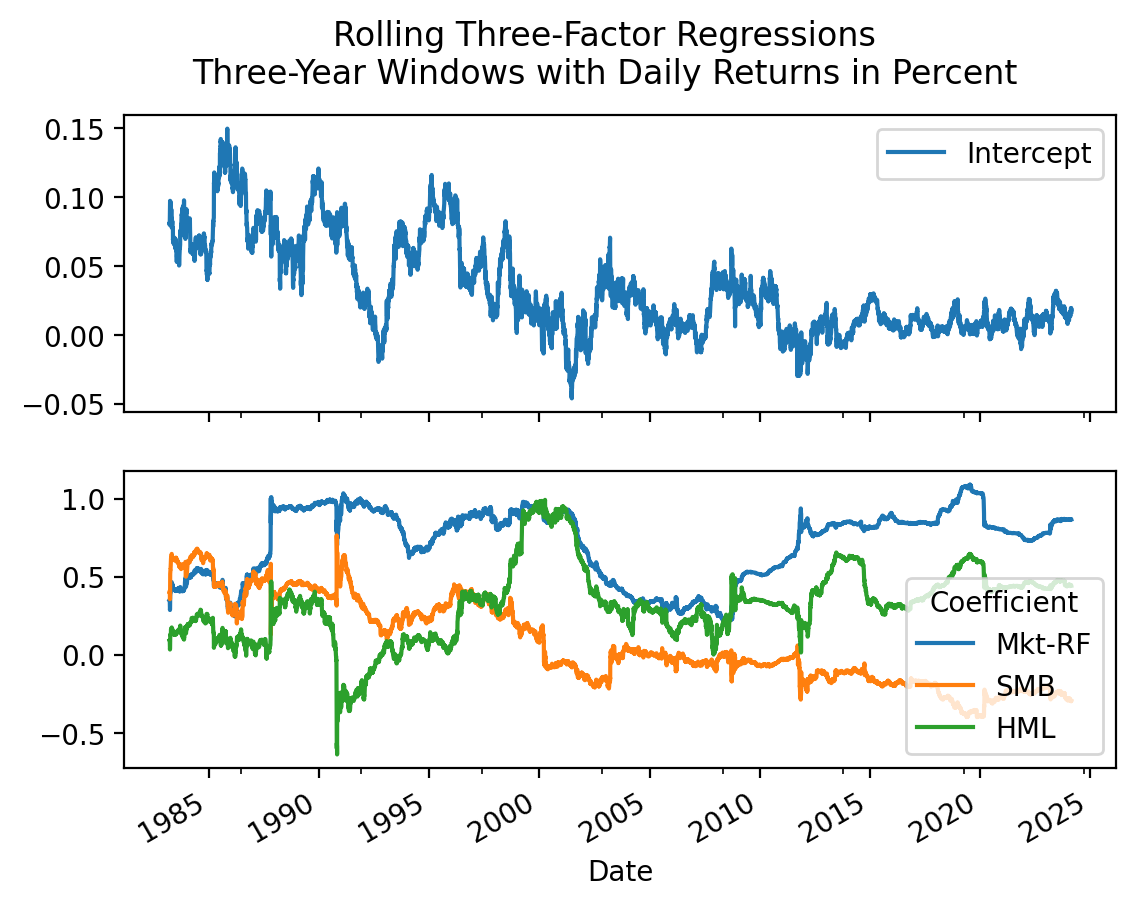
\includegraphics{mckinney_11_lecture_files/figure-pdf/cell-67-output-1.png}

}

\end{figure}

\hypertarget{user-defined-moving-window-functions}{%
\subsection{User-Defined Moving Window
Functions}\label{user-defined-moving-window-functions}}

Finally, we can define our own moving window functions and use the
\texttt{.apply()} method to apply them However, note that
\texttt{.apply()} will be much slower than the the optimized moving
window functions (e.g., \texttt{.mean()}, \texttt{.std()}, etc.).

McKinney provides an abstract example here, but we will discuss a
simpler example that calculates rolling volatility. Also, calculating
rolling volatility with the \texttt{.apply()} method provides us a
chance to benchmark it against the optimized version.

\begin{Shaded}
\begin{Highlighting}[]
\NormalTok{returns[}\StringTok{\textquotesingle{}AAPL\textquotesingle{}}\NormalTok{].rolling(}\DecValTok{252}\NormalTok{).}\BuiltInTok{apply}\NormalTok{(np.std).mul(np.sqrt(}\DecValTok{252}\NormalTok{) }\OperatorTok{*} \DecValTok{100}\NormalTok{).plot() }\CommentTok{\# annualize and convert to percent}
\NormalTok{plt.ylabel(}\StringTok{\textquotesingle{}Volatility (\%)\textquotesingle{}}\NormalTok{)}
\NormalTok{plt.title(}\StringTok{\textquotesingle{}Rolling Volatility}\CharTok{\textbackslash{}n}\StringTok{ (252{-}Day Window w/ 252{-}Day Minimum)\textquotesingle{}}\NormalTok{)}
\NormalTok{plt.show()}
\end{Highlighting}
\end{Shaded}

\begin{figure}[H]

{\centering \includegraphics{mckinney_11_lecture_files/figure-pdf/cell-68-output-1.png}

}

\end{figure}

Do not be afraid to use \texttt{.apply()}, but realize that
\texttt{.apply()} is typically 1000-times slower than the pre-built
method.

\begin{Shaded}
\begin{Highlighting}[]
\OperatorTok{\%}\NormalTok{timeit returns[}\StringTok{\textquotesingle{}AAPL\textquotesingle{}}\NormalTok{].rolling(}\DecValTok{252}\NormalTok{).}\BuiltInTok{apply}\NormalTok{(np.std)}
\end{Highlighting}
\end{Shaded}

\begin{verbatim}
936 ms ± 160 ms per loop (mean ± std. dev. of 7 runs, 1 loop each)
\end{verbatim}

\begin{Shaded}
\begin{Highlighting}[]
\OperatorTok{\%}\NormalTok{timeit returns[}\StringTok{\textquotesingle{}AAPL\textquotesingle{}}\NormalTok{].rolling(}\DecValTok{252}\NormalTok{).std()}
\end{Highlighting}
\end{Shaded}

\begin{verbatim}
337 µs ± 58 µs per loop (mean ± std. dev. of 7 runs, 1,000 loops each)
\end{verbatim}

\hypertarget{mckinney-chapter-11---practice-for-section-02}{%
\chapter{McKinney Chapter 11 - Practice for Section
02}\label{mckinney-chapter-11---practice-for-section-02}}

\hypertarget{announcements-28}{%
\section{Announcements}\label{announcements-28}}

\hypertarget{practice-28}{%
\section{Practice}\label{practice-28}}

\hypertarget{cumulative-returns-with-all-available-data}{%
\subsection{Cumulative returns with all available
data}\label{cumulative-returns-with-all-available-data}}

\hypertarget{total-returns-for-each-calendar-year}{%
\subsection{Total returns for each calendar
year}\label{total-returns-for-each-calendar-year}}

\hypertarget{total-returns-over-rolling-252-trading-day-windows}{%
\subsection{Total returns over rolling 252-trading-day
windows}\label{total-returns-over-rolling-252-trading-day-windows}}

\hypertarget{total-returns-over-rolling-12-months-windows-after-calculating-monthly-returns}{%
\subsection{Total returns over rolling 12-months windows after
calculating monthly
returns}\label{total-returns-over-rolling-12-months-windows-after-calculating-monthly-returns}}

\hypertarget{sharpe-ratios-for-each-calendar-year}{%
\subsection{Sharpe Ratios for each calendar
year}\label{sharpe-ratios-for-each-calendar-year}}

\hypertarget{calculate-rolling-betas}{%
\subsection{Calculate rolling betas}\label{calculate-rolling-betas}}

Calculate rolling capital asset pricing model (CAPM) betas for the
MATANA stocks.

The CAPM says the risk premium on a stock depends on the risk-free rate,
beta, and the risk premium on the market:
\(E(R_{stock}) = R_f + \beta_{stock} \times (E(R_{market}) - R_f)\). We
can calculate CAPM betas as:
\(\beta_{stock} = \frac{Cov(R_{stock} - R_f, R_{market} - R_f)}{Var(R_{market} - R_f)}\).

\hypertarget{calculate-rolling-sharpe-ratios}{%
\subsection{Calculate rolling Sharpe
Ratios}\label{calculate-rolling-sharpe-ratios}}

Calculate rolling Sharpe Ratios for the MATANA stocks.

The Sharpe Ratio is often used to evaluate fund managers. The Sharpe
Ratio is \(SR_i = \frac{\overline{R_i - R_f}}{\sigma}\), where
\(\overline{R_i-R_f}\) is mean fund return relative to the risk-free
rate over some period and \(\sigma\) is the standard deviation of
\(R_i-R_f\) over the same period. While the Sharpe Ratio is typically
used for funds, we can apply it to a single stock to test our knowledge
of the \texttt{.rolling()} method. Calculate and plot the one-year
rolling Sharpe Ratio for the MATANA stocks using all available daily
data.

\hypertarget{mckinney-chapter-11---practice-for-section-03}{%
\chapter{McKinney Chapter 11 - Practice for Section
03}\label{mckinney-chapter-11---practice-for-section-03}}

\hypertarget{announcements-29}{%
\section{Announcements}\label{announcements-29}}

\hypertarget{practice-29}{%
\section{Practice}\label{practice-29}}

\hypertarget{cumulative-returns-with-all-available-data-1}{%
\subsection{Cumulative returns with all available
data}\label{cumulative-returns-with-all-available-data-1}}

\hypertarget{total-returns-for-each-calendar-year-1}{%
\subsection{Total returns for each calendar
year}\label{total-returns-for-each-calendar-year-1}}

\hypertarget{total-returns-over-rolling-252-trading-day-windows-1}{%
\subsection{Total returns over rolling 252-trading-day
windows}\label{total-returns-over-rolling-252-trading-day-windows-1}}

\hypertarget{total-returns-over-rolling-12-months-windows-after-calculating-monthly-returns-1}{%
\subsection{Total returns over rolling 12-months windows after
calculating monthly
returns}\label{total-returns-over-rolling-12-months-windows-after-calculating-monthly-returns-1}}

\hypertarget{sharpe-ratios-for-each-calendar-year-1}{%
\subsection{Sharpe Ratios for each calendar
year}\label{sharpe-ratios-for-each-calendar-year-1}}

\hypertarget{calculate-rolling-betas-1}{%
\subsection{Calculate rolling betas}\label{calculate-rolling-betas-1}}

Calculate rolling capital asset pricing model (CAPM) betas for the
MATANA stocks.

The CAPM says the risk premium on a stock depends on the risk-free rate,
beta, and the risk premium on the market:
\(E(R_{stock}) = R_f + \beta_{stock} \times (E(R_{market}) - R_f)\). We
can calculate CAPM betas as:
\(\beta_{stock} = \frac{Cov(R_{stock} - R_f, R_{market} - R_f)}{Var(R_{market} - R_f)}\).

\hypertarget{calculate-rolling-sharpe-ratios-1}{%
\subsection{Calculate rolling Sharpe
Ratios}\label{calculate-rolling-sharpe-ratios-1}}

Calculate rolling Sharpe Ratios for the MATANA stocks.

The Sharpe Ratio is often used to evaluate fund managers. The Sharpe
Ratio is \(SR_i = \frac{\overline{R_i - R_f}}{\sigma}\), where
\(\overline{R_i-R_f}\) is mean fund return relative to the risk-free
rate over some period and \(\sigma\) is the standard deviation of
\(R_i-R_f\) over the same period. While the Sharpe Ratio is typically
used for funds, we can apply it to a single stock to test our knowledge
of the \texttt{.rolling()} method. Calculate and plot the one-year
rolling Sharpe Ratio for the MATANA stocks using all available daily
data.

\hypertarget{mckinney-chapter-11---practice-for-section-04}{%
\chapter{McKinney Chapter 11 - Practice for Section
04}\label{mckinney-chapter-11---practice-for-section-04}}

\hypertarget{announcements-30}{%
\section{Announcements}\label{announcements-30}}

\hypertarget{practice-30}{%
\section{Practice}\label{practice-30}}

\hypertarget{cumulative-returns-with-all-available-data-2}{%
\subsection{Cumulative returns with all available
data}\label{cumulative-returns-with-all-available-data-2}}

\hypertarget{total-returns-for-each-calendar-year-2}{%
\subsection{Total returns for each calendar
year}\label{total-returns-for-each-calendar-year-2}}

\hypertarget{total-returns-over-rolling-252-trading-day-windows-2}{%
\subsection{Total returns over rolling 252-trading-day
windows}\label{total-returns-over-rolling-252-trading-day-windows-2}}

\hypertarget{total-returns-over-rolling-12-months-windows-after-calculating-monthly-returns-2}{%
\subsection{Total returns over rolling 12-months windows after
calculating monthly
returns}\label{total-returns-over-rolling-12-months-windows-after-calculating-monthly-returns-2}}

\hypertarget{sharpe-ratios-for-each-calendar-year-2}{%
\subsection{Sharpe Ratios for each calendar
year}\label{sharpe-ratios-for-each-calendar-year-2}}

\hypertarget{calculate-rolling-betas-2}{%
\subsection{Calculate rolling betas}\label{calculate-rolling-betas-2}}

Calculate rolling capital asset pricing model (CAPM) betas for the
MATANA stocks.

The CAPM says the risk premium on a stock depends on the risk-free rate,
beta, and the risk premium on the market:
\(E(R_{stock}) = R_f + \beta_{stock} \times (E(R_{market}) - R_f)\). We
can calculate CAPM betas as:
\(\beta_{stock} = \frac{Cov(R_{stock} - R_f, R_{market} - R_f)}{Var(R_{market} - R_f)}\).

\hypertarget{calculate-rolling-sharpe-ratios-2}{%
\subsection{Calculate rolling Sharpe
Ratios}\label{calculate-rolling-sharpe-ratios-2}}

Calculate rolling Sharpe Ratios for the MATANA stocks.

The Sharpe Ratio is often used to evaluate fund managers. The Sharpe
Ratio is \(SR_i = \frac{\overline{R_i - R_f}}{\sigma}\), where
\(\overline{R_i-R_f}\) is mean fund return relative to the risk-free
rate over some period and \(\sigma\) is the standard deviation of
\(R_i-R_f\) over the same period. While the Sharpe Ratio is typically
used for funds, we can apply it to a single stock to test our knowledge
of the \texttt{.rolling()} method. Calculate and plot the one-year
rolling Sharpe Ratio for the MATANA stocks using all available daily
data.

\hypertarget{mckinney-chapter-11---practice-for-section-05}{%
\chapter{McKinney Chapter 11 - Practice for Section
05}\label{mckinney-chapter-11---practice-for-section-05}}

\hypertarget{announcements-31}{%
\section{Announcements}\label{announcements-31}}

\hypertarget{practice-31}{%
\section{Practice}\label{practice-31}}

\hypertarget{cumulative-returns-with-all-available-data-3}{%
\subsection{Cumulative returns with all available
data}\label{cumulative-returns-with-all-available-data-3}}

\hypertarget{total-returns-for-each-calendar-year-3}{%
\subsection{Total returns for each calendar
year}\label{total-returns-for-each-calendar-year-3}}

\hypertarget{total-returns-over-rolling-252-trading-day-windows-3}{%
\subsection{Total returns over rolling 252-trading-day
windows}\label{total-returns-over-rolling-252-trading-day-windows-3}}

\hypertarget{total-returns-over-rolling-12-months-windows-after-calculating-monthly-returns-3}{%
\subsection{Total returns over rolling 12-months windows after
calculating monthly
returns}\label{total-returns-over-rolling-12-months-windows-after-calculating-monthly-returns-3}}

\hypertarget{sharpe-ratios-for-each-calendar-year-3}{%
\subsection{Sharpe Ratios for each calendar
year}\label{sharpe-ratios-for-each-calendar-year-3}}

\hypertarget{calculate-rolling-betas-3}{%
\subsection{Calculate rolling betas}\label{calculate-rolling-betas-3}}

Calculate rolling capital asset pricing model (CAPM) betas for the
MATANA stocks.

The CAPM says the risk premium on a stock depends on the risk-free rate,
beta, and the risk premium on the market:
\(E(R_{stock}) = R_f + \beta_{stock} \times (E(R_{market}) - R_f)\). We
can calculate CAPM betas as:
\(\beta_{stock} = \frac{Cov(R_{stock} - R_f, R_{market} - R_f)}{Var(R_{market} - R_f)}\).

\hypertarget{calculate-rolling-sharpe-ratios-3}{%
\subsection{Calculate rolling Sharpe
Ratios}\label{calculate-rolling-sharpe-ratios-3}}

Calculate rolling Sharpe Ratios for the MATANA stocks.

The Sharpe Ratio is often used to evaluate fund managers. The Sharpe
Ratio is \(SR_i = \frac{\overline{R_i - R_f}}{\sigma}\), where
\(\overline{R_i-R_f}\) is mean fund return relative to the risk-free
rate over some period and \(\sigma\) is the standard deviation of
\(R_i-R_f\) over the same period. While the Sharpe Ratio is typically
used for funds, we can apply it to a single stock to test our knowledge
of the \texttt{.rolling()} method. Calculate and plot the one-year
rolling Sharpe Ratio for the MATANA stocks using all available daily
data.

\part{Week 10}

\hypertarget{herron-topic-2---trading-strategies}{%
\chapter{Herron Topic 2 - Trading
Strategies}\label{herron-topic-2---trading-strategies}}

This notebook covers trading strategies based on technical analysis in
three parts:

\begin{enumerate}
\def\labelenumi{\arabic{enumi}.}
\tightlist
\item
  What is technical analysis?
\item
  Why might trading strategies based on technical analysis work (or not
  work)?
\item
  Implement a simple moving average (SMA) trading strategy
\end{enumerate}

I based this lecture notebook on
\href{https://book.ivo-welch.info/read/source5.mba/12-effbehav.pdf}{chapter
12 of Ivo Welch's \emph{Corporate Finance} textbook} and chapter 2 of
\href{https://onesearch.library.northeastern.edu/permalink/01NEU_INST/i2gqis/alma9952082522901401}{Eryk
Lewinson's \emph{Python for Finance Cookbook}}. The practice notebook
will cover several other trading strategies based on technical analysis.

\begin{Shaded}
\begin{Highlighting}[]
\ImportTok{import}\NormalTok{ matplotlib.pyplot }\ImportTok{as}\NormalTok{ plt}
\ImportTok{import}\NormalTok{ numpy }\ImportTok{as}\NormalTok{ np}
\ImportTok{import}\NormalTok{ pandas }\ImportTok{as}\NormalTok{ pd}
\end{Highlighting}
\end{Shaded}

\begin{Shaded}
\begin{Highlighting}[]
\OperatorTok{\%}\NormalTok{precision }\DecValTok{4}
\NormalTok{pd.options.display.float\_format }\OperatorTok{=} \StringTok{\textquotesingle{}}\SpecialCharTok{\{:.4f\}}\StringTok{\textquotesingle{}}\NormalTok{.}\BuiltInTok{format}
\OperatorTok{\%}\NormalTok{config InlineBackend.figure\_format }\OperatorTok{=} \StringTok{\textquotesingle{}retina\textquotesingle{}}
\end{Highlighting}
\end{Shaded}

\hypertarget{what-is-technical-analysis}{%
\section{What is technical analysis?}\label{what-is-technical-analysis}}

\href{https://en.wikipedia.org/wiki/Technical_analysis}{Technical
analysis} is a methodology that analyzes past market data (e.g., past
prices and volume) in an attempt to forecast future price movements. If
technical analysis can predict future price movements, the market is not
weak-form efficient. Ivo Welch provides the three degrees of market
efficiency in section 12.2 of
\href{https://book.ivo-welch.info/read/source5.mba/12-effbehav.pdf}{chapter
12 of his (free) \emph{Corporate Finance} textbook}:

\begin{quote}
The Traditional Classification The traditional definition of market
efficiency focuses on information. In the traditional classification,
market efficiency comes in one of three primary degrees: weak,
semi-strong, and strong.

\textbf{Weak market efficiency} says that all information in past prices
is reflected in today's stock prices so that technical analysis (trading
based solely on historical price patterns) cannot be used to beat the
market. Put differently, the market is the best technical analyst.

\textbf{Semistrong market efficiency} says that all public information
is reflected in today's stock prices, so that neither fundamental
trading (based on underlying firm fundamentals, such as cash flows or
discount rates) nor technical analysis can be used to beat the market.
Put differently, the market is both the best technical and the best
fundamental analyst.

\textbf{Strong market efficiency} says that all information, both public
and private, is reflected in today's stock prices, so that nothing ---
not even private insider information --- can be used to beat the market.
Put differently, the market is the best analyst and cannot be beat.

In this traditional classification, all finance professors most U.S.
financial markets are not strong-form efficient: Insider trading may be
illegal, but it works. However, there are still arguments as to which
markets are only semi-strong-form efficient or even only weak-form
efficient.
\end{quote}

Section 12.2 goes on to provide Welch's own taxonomy of true, firm,
mild, and nonbelievers in market efficiency. Chapter 12 summarizes
market efficiency, classical finance, behavioral finance, arbitrage,
limits to arbitrage, and their consequences for managers and investors.
We will focus on technical analysis in this notebook, but chapter 12 is
excellent.

\hypertarget{why-might-trading-strategies-based-on-technical-analysis-work-or-not}{%
\section{Why might trading strategies based on technical analysis work
or
not?}\label{why-might-trading-strategies-based-on-technical-analysis-work-or-not}}

\hypertarget{work}{%
\subsection{\ldots Work?}\label{work}}

Technical analysis relies on a few ideas:

\begin{enumerate}
\def\labelenumi{\arabic{enumi}.}
\tightlist
\item
  Market prices and volume reflect all relevant information, so we can
  focus on past prices and volume instead of fundamentals and news.
\item
  Market prices move in trends and patterns driven by market
  participants.
\item
  These trends and patterns tend to repeat themselves because market
  participants create them.
\end{enumerate}

\hypertarget{or-not}{%
\subsection{\ldots Or Not?}\label{or-not}}

The logic above is reasonable. However, if past market prices reflect
all relevant information, they should also reflect any prices trends
they predict. Therefore, any patterns should be self-defeating, and
market prices should follow
\href{https://en.wikipedia.org/wiki/Random_walk_hypothesis}{a random
walk}. As well, the signal-to-noise ratio in market prices is high!
Still, technical analysis provides an opportunity to learn how to
implement and back-test trading strategies in Python.

\hypertarget{a-random-walk}{%
\subsubsection{A Random Walk}\label{a-random-walk}}

In a random walk, the price tomorrow equals the price today plus a tiny
drift plus noise. In math terms, a random walk is
\(P_{t} = \rho P_{t-1} + m P_{t-1} + \varepsilon\), where \(m\) is a
small drift term and \(E[\varepsilon] = 0\). If \(\rho > 1\), prices
would quickly increase, and, if \(\rho < 1\), prices would quickly
decrease. Let us examine the historical record.

\begin{Shaded}
\begin{Highlighting}[]
\ImportTok{import}\NormalTok{ pandas\_datareader }\ImportTok{as}\NormalTok{ pdr}
\end{Highlighting}
\end{Shaded}

\begin{Shaded}
\begin{Highlighting}[]
\NormalTok{ff }\OperatorTok{=}\NormalTok{ (}
\NormalTok{    pdr.DataReader(}
\NormalTok{        name}\OperatorTok{=}\StringTok{\textquotesingle{}F{-}F\_Research\_Data\_Factors\_daily\textquotesingle{}}\NormalTok{,}
\NormalTok{        data\_source}\OperatorTok{=}\StringTok{\textquotesingle{}famafrench\textquotesingle{}}\NormalTok{,}
\NormalTok{        start}\OperatorTok{=}\StringTok{\textquotesingle{}1900\textquotesingle{}}
\NormalTok{    )}
\NormalTok{    [}\DecValTok{0}\NormalTok{]}
\NormalTok{    .assign(Mkt }\OperatorTok{=} \KeywordTok{lambda}\NormalTok{ x: x[}\StringTok{\textquotesingle{}Mkt{-}RF\textquotesingle{}}\NormalTok{] }\OperatorTok{+}\NormalTok{ x[}\StringTok{\textquotesingle{}RF\textquotesingle{}}\NormalTok{])}
\NormalTok{    .div(}\DecValTok{100}\NormalTok{)}
\NormalTok{)}

\NormalTok{ff.head()}
\end{Highlighting}
\end{Shaded}

\begin{verbatim}
C:\Users\r.herron\AppData\Local\Temp\ipykernel_14600\3181934010.py:2: FutureWarning: The argument 'date_parser' is deprecated and will be removed in a future version. Please use 'date_format' instead, or read your data in as 'object' dtype and then call 'to_datetime'.
  pdr.DataReader(
\end{verbatim}

\begin{longtable}[]{@{}llllll@{}}
\toprule\noalign{}
& Mkt-RF & SMB & HML & RF & Mkt \\
Date & & & & & \\
\midrule\noalign{}
\endhead
\bottomrule\noalign{}
\endlastfoot
1926-07-01 & 0.0010 & -0.0025 & -0.0027 & 0.0001 & 0.0011 \\
1926-07-02 & 0.0045 & -0.0033 & -0.0006 & 0.0001 & 0.0046 \\
1926-07-06 & 0.0017 & 0.0030 & -0.0039 & 0.0001 & 0.0018 \\
1926-07-07 & 0.0009 & -0.0058 & 0.0002 & 0.0001 & 0.0010 \\
1926-07-08 & 0.0021 & -0.0038 & 0.0019 & 0.0001 & 0.0022 \\
\end{longtable}

We can use market returns to impute market prices relative to the last
day of June 1926.

\begin{Shaded}
\begin{Highlighting}[]
\NormalTok{price }\OperatorTok{=}\NormalTok{ ff[}\StringTok{\textquotesingle{}Mkt\textquotesingle{}}\NormalTok{].add(}\DecValTok{1}\NormalTok{).cumprod()}

\NormalTok{price.tail()}
\end{Highlighting}
\end{Shaded}

\begin{verbatim}
Date
2023-10-25   10168.8352
2023-10-26   10054.0290
2023-10-27   10002.8540
2023-10-30   10119.9874
2023-10-31   10185.8686
Name: Mkt, dtype: float64
\end{verbatim}

\begin{Shaded}
\begin{Highlighting}[]
\NormalTok{price.plot()}
\NormalTok{plt.title(}\StringTok{\textquotesingle{}Imputed Market Prices}\CharTok{\textbackslash{}n}\StringTok{Assuming $1 on the Last Day of June 1926\textquotesingle{}}\NormalTok{)}
\NormalTok{plt.ylabel(}\StringTok{\textquotesingle{}Imputed Market Price ($)\textquotesingle{}}\NormalTok{)}
\NormalTok{plt.semilogy()}
\NormalTok{plt.show()}
\end{Highlighting}
\end{Shaded}

\begin{figure}[H]

{\centering \includegraphics{herron_02_lecture_files/figure-pdf/cell-7-output-1.png}

}

\end{figure}

We need lagged prices to estimate \(\rho\). We will add 10 lags of \(P\)
to help us understand the relation between past and future prices.

\begin{Shaded}
\begin{Highlighting}[]
\NormalTok{price\_lags }\OperatorTok{=}\NormalTok{ (}
\NormalTok{    pd.concat(}
\NormalTok{        objs}\OperatorTok{=}\NormalTok{[price.shift(t) }\ControlFlowTok{for}\NormalTok{ t }\KeywordTok{in} \BuiltInTok{range}\NormalTok{(}\DecValTok{11}\NormalTok{)],}
\NormalTok{        keys}\OperatorTok{=}\NormalTok{[}\SpecialStringTok{f\textquotesingle{}Lag }\SpecialCharTok{\{}\NormalTok{t}\SpecialCharTok{\}}\SpecialStringTok{\textquotesingle{}} \ControlFlowTok{for}\NormalTok{ t }\KeywordTok{in} \BuiltInTok{range}\NormalTok{(}\DecValTok{11}\NormalTok{)],}
\NormalTok{        names}\OperatorTok{=}\NormalTok{[}\StringTok{\textquotesingle{}Price\textquotesingle{}}\NormalTok{],}
\NormalTok{        axis}\OperatorTok{=}\DecValTok{1}\NormalTok{,}
\NormalTok{    )}
\NormalTok{)}

\NormalTok{price\_lags.head()}
\end{Highlighting}
\end{Shaded}

\begin{longtable}[]{@{}llllllllllll@{}}
\toprule\noalign{}
Price & Lag 0 & Lag 1 & Lag 2 & Lag 3 & Lag 4 & Lag 5 & Lag 6 & Lag 7 &
Lag 8 & Lag 9 & Lag 10 \\
Date & & & & & & & & & & & \\
\midrule\noalign{}
\endhead
\bottomrule\noalign{}
\endlastfoot
1926-07-01 & 1.0011 & NaN & NaN & NaN & NaN & NaN & NaN & NaN & NaN &
NaN & NaN \\
1926-07-02 & 1.0057 & 1.0011 & NaN & NaN & NaN & NaN & NaN & NaN & NaN &
NaN & NaN \\
1926-07-06 & 1.0075 & 1.0057 & 1.0011 & NaN & NaN & NaN & NaN & NaN &
NaN & NaN & NaN \\
1926-07-07 & 1.0085 & 1.0075 & 1.0057 & 1.0011 & NaN & NaN & NaN & NaN &
NaN & NaN & NaN \\
1926-07-08 & 1.0107 & 1.0085 & 1.0075 & 1.0057 & 1.0011 & NaN & NaN &
NaN & NaN & NaN & NaN \\
\end{longtable}

\begin{Shaded}
\begin{Highlighting}[]
\NormalTok{(}
\NormalTok{    price\_lags}
\NormalTok{    .dropna()}
\NormalTok{    .corr()}
\NormalTok{    .loc[}\StringTok{\textquotesingle{}Lag 0\textquotesingle{}}\NormalTok{]}
\NormalTok{    .plot(kind}\OperatorTok{=}\StringTok{\textquotesingle{}bar\textquotesingle{}}\NormalTok{)}
\NormalTok{)}
\NormalTok{plt.title(}\StringTok{\textquotesingle{}Correlations with Imputed Market Price\textquotesingle{}}\NormalTok{)}
\NormalTok{plt.ylabel(}\StringTok{\textquotesingle{}Correlation\textquotesingle{}}\NormalTok{)}
\NormalTok{plt.show()}
\end{Highlighting}
\end{Shaded}

\begin{figure}[H]

{\centering \includegraphics{herron_02_lecture_files/figure-pdf/cell-9-output-1.png}

}

\end{figure}

But these are \emph{pairwise} correlations. If we estimate
\emph{conditional} correlations, we see that most of the price
information is in the first lag!

\begin{Shaded}
\begin{Highlighting}[]
\ImportTok{import}\NormalTok{ statsmodels.api }\ImportTok{as}\NormalTok{ sm}
\end{Highlighting}
\end{Shaded}

\begin{Shaded}
\begin{Highlighting}[]
\NormalTok{\_ }\OperatorTok{=}\NormalTok{ price\_lags.dropna()}
\NormalTok{y }\OperatorTok{=}\NormalTok{ \_[}\StringTok{\textquotesingle{}Lag 0\textquotesingle{}}\NormalTok{]}
\NormalTok{X }\OperatorTok{=}\NormalTok{ \_.drop(}\StringTok{\textquotesingle{}Lag 0\textquotesingle{}}\NormalTok{, axis}\OperatorTok{=}\DecValTok{1}\NormalTok{).pipe(sm.add\_constant)}
\NormalTok{model }\OperatorTok{=}\NormalTok{ sm.OLS(endog}\OperatorTok{=}\NormalTok{y, exog}\OperatorTok{=}\NormalTok{X)}
\NormalTok{fit }\OperatorTok{=}\NormalTok{ model.fit(cov\_type}\OperatorTok{=}\StringTok{\textquotesingle{}HAC\textquotesingle{}}\NormalTok{, cov\_kwds}\OperatorTok{=}\NormalTok{\{}\StringTok{\textquotesingle{}maxlags\textquotesingle{}}\NormalTok{: }\DecValTok{10}\NormalTok{\})}
\NormalTok{fit.summary()}
\end{Highlighting}
\end{Shaded}

\begin{center}
\begin{tabular}{lclc}
\toprule
\textbf{Dep. Variable:}    &      Lag 0       & \textbf{  R-squared:         } &      1.000   \\
\textbf{Model:}            &       OLS        & \textbf{  Adj. R-squared:    } &      1.000   \\
\textbf{Method:}           &  Least Squares   & \textbf{  F-statistic:       } &  1.768e+06   \\
\textbf{Date:}             & Fri, 22 Dec 2023 & \textbf{  Prob (F-statistic):} &      0.00    \\
\textbf{Time:}             &     10:00:20     & \textbf{  Log-Likelihood:    } & -1.2187e+05  \\
\textbf{No. Observations:} &       25598      & \textbf{  AIC:               } &  2.438e+05   \\
\textbf{Df Residuals:}     &       25587      & \textbf{  BIC:               } &  2.438e+05   \\
\textbf{Df Model:}         &          10      & \textbf{                     } &              \\
\textbf{Covariance Type:}  &       HAC        & \textbf{                     } &              \\
\bottomrule
\end{tabular}
\begin{tabular}{lcccccc}
                & \textbf{coef} & \textbf{std err} & \textbf{z} & \textbf{P$> |$z$|$} & \textbf{[0.025} & \textbf{0.975]}  \\
\midrule
\textbf{const}  &       0.1283  &        0.145     &     0.888  &         0.375        &       -0.155    &        0.412     \\
\textbf{Lag 1}  &       0.9447  &        0.035     &    26.932  &         0.000        &        0.876    &        1.013     \\
\textbf{Lag 2}  &       0.0764  &        0.061     &     1.256  &         0.209        &       -0.043    &        0.196     \\
\textbf{Lag 3}  &      -0.0311  &        0.039     &    -0.805  &         0.421        &       -0.107    &        0.045     \\
\textbf{Lag 4}  &      -0.0268  &        0.043     &    -0.618  &         0.536        &       -0.112    &        0.058     \\
\textbf{Lag 5}  &       0.0477  &        0.040     &     1.187  &         0.235        &       -0.031    &        0.127     \\
\textbf{Lag 6}  &      -0.0706  &        0.043     &    -1.651  &         0.099        &       -0.154    &        0.013     \\
\textbf{Lag 7}  &       0.1277  &        0.050     &     2.548  &         0.011        &        0.029    &        0.226     \\
\textbf{Lag 8}  &      -0.1339  &        0.056     &    -2.373  &         0.018        &       -0.244    &       -0.023     \\
\textbf{Lag 9}  &       0.1552  &        0.048     &     3.215  &         0.001        &        0.061    &        0.250     \\
\textbf{Lag 10} &      -0.0890  &        0.033     &    -2.729  &         0.006        &       -0.153    &       -0.025     \\
\bottomrule
\end{tabular}
\begin{tabular}{lclc}
\textbf{Omnibus:}       & 16175.844 & \textbf{  Durbin-Watson:     } &      1.995   \\
\textbf{Prob(Omnibus):} &    0.000  & \textbf{  Jarque-Bera (JB):  } & 5235480.028  \\
\textbf{Skew:}          &   -1.860  & \textbf{  Prob(JB):          } &       0.00   \\
\textbf{Kurtosis:}      &   72.963  & \textbf{  Cond. No.          } &   8.70e+03   \\
\bottomrule
\end{tabular}
%\caption{OLS Regression Results}
\end{center}

Notes: \newline
 [1] Standard Errors are heteroscedasticity and autocorrelation robust (HAC) using 10 lags and without small sample correction \newline
 [2] The condition number is large, 8.7e+03. This might indicate that there are \newline
 strong multicollinearity or other numerical problems.

\begin{Shaded}
\begin{Highlighting}[]
\NormalTok{plt.bar(}
\NormalTok{    x}\OperatorTok{=}\NormalTok{price\_lags.columns[}\DecValTok{1}\NormalTok{:],}
\NormalTok{    height}\OperatorTok{=}\NormalTok{fit.params[}\DecValTok{1}\NormalTok{:],}
\NormalTok{    yerr}\OperatorTok{=}\DecValTok{2}\OperatorTok{*}\NormalTok{fit.bse[}\DecValTok{1}\NormalTok{:]}
\NormalTok{)}
\NormalTok{plt.title(}\StringTok{\textquotesingle{}Conditional Correlations with Imputed Market Price}\CharTok{\textbackslash{}n}\StringTok{Bars Indicate $\textbackslash{}pm 2$ Standard Errors\textquotesingle{}}\NormalTok{)}
\NormalTok{plt.ylabel(}\StringTok{\textquotesingle{}Conditional Correlation\textquotesingle{}}\NormalTok{)}
\NormalTok{plt.xlabel(}\StringTok{\textquotesingle{}Price\textquotesingle{}}\NormalTok{)}
\NormalTok{plt.show()}
\end{Highlighting}
\end{Shaded}

\begin{figure}[H]

{\centering \includegraphics{herron_02_lecture_files/figure-pdf/cell-12-output-1.png}

}

\end{figure}

\hypertarget{signal-to-noise-ratio}{%
\subsubsection{Signal-to-Noise Ratio}\label{signal-to-noise-ratio}}

Recall, we can express a random walk as
\(P_{t} = \rho P_{t-1} + m P_{t-1} + \varepsilon_t\). Since
\(\rho = 1\), we can subtract \(P_{t-1}\) from both sides, then divide
by \(P_{t-1}\) on both sides. This transformation expresses a random
walk in terms of returns: \(r_{t-1,t} = m + e_t\), where \(E[e_t] = 0\)
and \(SD[e_t] = s\), so \(E[r_{t-1, t}] = m\). We can think of the
signal-to-noise ratio as \(\frac{m}{s}\). How high is this ratio?

\begin{Shaded}
\begin{Highlighting}[]
\NormalTok{m, s }\OperatorTok{=}\NormalTok{ ff[}\StringTok{\textquotesingle{}Mkt\textquotesingle{}}\NormalTok{].mean(), ff[}\StringTok{\textquotesingle{}Mkt\textquotesingle{}}\NormalTok{].std()}
\end{Highlighting}
\end{Shaded}

Here \(m\) is about 4 basis points per day!

\begin{Shaded}
\begin{Highlighting}[]
\NormalTok{m}
\end{Highlighting}
\end{Shaded}

\begin{verbatim}
0.0004
\end{verbatim}

However, \(s\) is about 108 basis points per day!

\begin{Shaded}
\begin{Highlighting}[]
\NormalTok{s}
\end{Highlighting}
\end{Shaded}

\begin{verbatim}
0.0108
\end{verbatim}

Therefore, the signal-to-noise ratio is less than 4 percent!

\begin{Shaded}
\begin{Highlighting}[]
\NormalTok{m}\OperatorTok{/}\NormalTok{s}
\end{Highlighting}
\end{Shaded}

\begin{verbatim}
0.0388
\end{verbatim}

Means grow linearly with time, while standard deviations growth with the
square-root of time. Therefore, even with a 1 basis point signal, we
need a lot of data to make sure this 1 basis point signal is real! For
example, if we want \(\sqrt{t} \times \frac{1}{s} \geq 2\), we need
\(t \geq \left(2 \times \frac{s}{1} \right)^2\) days! Even with market
noise, which is diversified and low, we need more than 100 years of
data!

\begin{Shaded}
\begin{Highlighting}[]
\NormalTok{(}\DecValTok{2} \OperatorTok{*}\NormalTok{ s }\OperatorTok{/} \FloatTok{0.0001}\NormalTok{)}\OperatorTok{**}\DecValTok{2} \OperatorTok{/} \DecValTok{365}
\end{Highlighting}
\end{Shaded}

\begin{verbatim}
128.0929
\end{verbatim}

\hypertarget{implement-a-simple-moving-average-sma-trading-strategy}{%
\section{Implement a simple moving average (SMA) trading
strategy}\label{implement-a-simple-moving-average-sma-trading-strategy}}

One goal of technical analysis is to ``buy low, and sell high''. The
\(n\)-day SMA reduces noise in market prices, removing market
fluctuations and providing estimates of ``true'' prices. Market prices
below their SMA might be buying opportunities, and market prices below
their SMA might be selling opportunities. Here, we will implement a
long-only 20-day SMA (SMA(20)) strategy with Bitcoin:

\begin{enumerate}
\def\labelenumi{\arabic{enumi}.}
\tightlist
\item
  Buy when the closing price crosses SMA(20) from below
\item
  Sell when the closing price crosses SMA(20) from above
\item
  No short-selling
\end{enumerate}

Because we will not sell short, we can simplify this strategy to ``long
if above SMA(20), otherwise neutral''. First, we will need Bitcoin
returns data.

\begin{Shaded}
\begin{Highlighting}[]
\ImportTok{import}\NormalTok{ yfinance }\ImportTok{as}\NormalTok{ yf}
\end{Highlighting}
\end{Shaded}

\begin{Shaded}
\begin{Highlighting}[]
\NormalTok{btc }\OperatorTok{=}\NormalTok{ (}
\NormalTok{    yf.download(tickers}\OperatorTok{=}\StringTok{\textquotesingle{}BTC{-}USD\textquotesingle{}}\NormalTok{)}
\NormalTok{    .assign(Return }\OperatorTok{=} \KeywordTok{lambda}\NormalTok{ x: x[}\StringTok{\textquotesingle{}Adj Close\textquotesingle{}}\NormalTok{].pct\_change())}
\NormalTok{    .rename\_axis(columns}\OperatorTok{=}\StringTok{\textquotesingle{}Variable\textquotesingle{}}\NormalTok{)}
\NormalTok{)}

\NormalTok{btc.head()}
\end{Highlighting}
\end{Shaded}

\begin{verbatim}
[*********************100%%**********************]  1 of 1 completed
\end{verbatim}

\begin{longtable}[]{@{}llllllll@{}}
\toprule\noalign{}
Variable & Open & High & Low & Close & Adj Close & Volume & Return \\
Date & & & & & & & \\
\midrule\noalign{}
\endhead
\bottomrule\noalign{}
\endlastfoot
2014-09-17 & 465.8640 & 468.1740 & 452.4220 & 457.3340 & 457.3340 &
21056800 & NaN \\
2014-09-18 & 456.8600 & 456.8600 & 413.1040 & 424.4400 & 424.4400 &
34483200 & -0.0719 \\
2014-09-19 & 424.1030 & 427.8350 & 384.5320 & 394.7960 & 394.7960 &
37919700 & -0.0698 \\
2014-09-20 & 394.6730 & 423.2960 & 389.8830 & 408.9040 & 408.9040 &
36863600 & 0.0357 \\
2014-09-21 & 408.0850 & 412.4260 & 393.1810 & 398.8210 & 398.8210 &
26580100 & -0.0247 \\
\end{longtable}

Next we:

\begin{enumerate}
\def\labelenumi{\arabic{enumi}.}
\tightlist
\item
  Use \texttt{.rolling(20).mean()} to add a \texttt{SMA20} column
  containing SMA(20) to our \texttt{btc} data frame
\item
  Use \texttt{np.select()} to add a \texttt{Position} column containing:

  \begin{enumerate}
  \def\labelenumii{\arabic{enumii}.}
  \tightlist
  \item
    \texttt{1} (long) when the adjusted close is greater than SMA(20)
  \item
    \texttt{0} (neutral) when the adjusted close is less than (or equal
    to) SMA(20)
  \item
    We could use \texttt{np.where()} instead of \texttt{np.select()},
    but using \texttt{np.select()} provides a more flexible framework
    for more complex examples
  \item
    \textbf{We use \texttt{.shift()} to compare yesterday's closing
    prices, avoiding a look-ahead bias}
  \end{enumerate}
\item
  Add a \texttt{Strategy} column containing:

  \begin{enumerate}
  \def\labelenumii{\arabic{enumii}.}
  \tightlist
  \item
    \texttt{Return} if \texttt{Position\ ==\ 1}
  \item
    \texttt{0} if \texttt{Position\ ==\ 0}
  \item
    We could earn the risk-free rate instead of 0 percent, but earning 0
    percent simplifies this example
  \end{enumerate}
\end{enumerate}

\begin{Shaded}
\begin{Highlighting}[]
\NormalTok{btc }\OperatorTok{=}\NormalTok{ (}
\NormalTok{    btc}
\NormalTok{    .assign(}
\NormalTok{        SMA20 }\OperatorTok{=} \KeywordTok{lambda}\NormalTok{ x: x[}\StringTok{\textquotesingle{}Adj Close\textquotesingle{}}\NormalTok{].rolling(}\DecValTok{20}\NormalTok{).mean(),}
\NormalTok{        Position }\OperatorTok{=} \KeywordTok{lambda}\NormalTok{ x: np.select(}
\NormalTok{            condlist}\OperatorTok{=}\NormalTok{[x[}\StringTok{\textquotesingle{}Adj Close\textquotesingle{}}\NormalTok{].shift() }\OperatorTok{\textgreater{}}\NormalTok{ x[}\StringTok{\textquotesingle{}SMA20\textquotesingle{}}\NormalTok{].shift(), x[}\StringTok{\textquotesingle{}Adj Close\textquotesingle{}}\NormalTok{].shift() }\OperatorTok{\textless{}=}\NormalTok{ x[}\StringTok{\textquotesingle{}SMA20\textquotesingle{}}\NormalTok{].shift()],}
\NormalTok{            choicelist}\OperatorTok{=}\NormalTok{[}\DecValTok{1}\NormalTok{, }\DecValTok{0}\NormalTok{],}
\NormalTok{            default}\OperatorTok{=}\NormalTok{np.nan}
\NormalTok{        ),}
\NormalTok{        Strategy }\OperatorTok{=} \KeywordTok{lambda}\NormalTok{ x: x[}\StringTok{\textquotesingle{}Position\textquotesingle{}}\NormalTok{] }\OperatorTok{*}\NormalTok{ x[}\StringTok{\textquotesingle{}Return\textquotesingle{}}\NormalTok{]}
\NormalTok{    )}
\NormalTok{)}

\NormalTok{btc.tail()}
\end{Highlighting}
\end{Shaded}

\begin{longtable}[]{@{}lllllllllll@{}}
\toprule\noalign{}
Variable & Open & High & Low & Close & Adj Close & Volume & Return &
SMA20 & Position & Strategy \\
Date & & & & & & & & & & \\
\midrule\noalign{}
\endhead
\bottomrule\noalign{}
\endlastfoot
2023-12-18 & 41348.2031 & 42720.2969 & 40530.2578 & 42623.5391 &
42623.5391 & 25224642008 & 0.0304 & 41762.6850 & 0.0000 & 0.0000 \\
2023-12-19 & 42641.5117 & 43354.2969 & 41826.3359 & 42270.5273 &
42270.5273 & 23171001281 & -0.0083 & 41983.2867 & 1.0000 & -0.0083 \\
2023-12-20 & 42261.3008 & 44275.5859 & 42223.8164 & 43652.2500 &
43652.2500 & 27868908174 & 0.0327 & 42280.2619 & 1.0000 & 0.0327 \\
2023-12-21 & 43648.1250 & 44240.6680 & 43330.0508 & 43869.1523 &
43869.1523 & 22452766169 & 0.0050 & 42539.2820 & 1.0000 & 0.0050 \\
2023-12-22 & 43868.9883 & 44367.9570 & 43441.9688 & 43665.7266 &
43665.7266 & 23145105408 & -0.0046 & 42748.7518 & 1.0000 & -0.0046 \\
\end{longtable}

I find it helpful to plot \texttt{Adj\ Close}, \texttt{SMA20}, and
\texttt{Position} for a sort window with one or more crossings.

\begin{Shaded}
\begin{Highlighting}[]
\NormalTok{fig, ax }\OperatorTok{=}\NormalTok{ plt.subplots(}\DecValTok{2}\NormalTok{, }\DecValTok{1}\NormalTok{, sharex}\OperatorTok{=}\VariableTok{True}\NormalTok{)}
\NormalTok{\_ }\OperatorTok{=}\NormalTok{ btc.loc[}\StringTok{\textquotesingle{}2023{-}02\textquotesingle{}}\NormalTok{].iloc[}\OperatorTok{{-}}\DecValTok{15}\NormalTok{:]}
\NormalTok{\_[[}\StringTok{\textquotesingle{}Adj Close\textquotesingle{}}\NormalTok{, }\StringTok{\textquotesingle{}SMA20\textquotesingle{}}\NormalTok{]].plot(ax}\OperatorTok{=}\NormalTok{ax[}\DecValTok{0}\NormalTok{], ylabel}\OperatorTok{=}\StringTok{\textquotesingle{}BTC{-}USD ($)\textquotesingle{}}\NormalTok{)}
\NormalTok{\_[[}\StringTok{\textquotesingle{}Position\textquotesingle{}}\NormalTok{]].plot(ax}\OperatorTok{=}\NormalTok{ax[}\DecValTok{1}\NormalTok{], ylabel}\OperatorTok{=}\StringTok{\textquotesingle{}Position\textquotesingle{}}\NormalTok{, legend}\OperatorTok{=}\VariableTok{False}\NormalTok{)}
\NormalTok{plt.suptitle(}\StringTok{\textquotesingle{}Bitcoin SMA(20) Strategy\textquotesingle{}}\NormalTok{)}
\NormalTok{plt.show()}
\end{Highlighting}
\end{Shaded}

\begin{figure}[H]

{\centering \includegraphics{herron_02_lecture_files/figure-pdf/cell-21-output-1.png}

}

\end{figure}

We can compare the long-run performance of buy-and-hold and SMA(20).

\begin{Shaded}
\begin{Highlighting}[]
\NormalTok{\_ }\OperatorTok{=}\NormalTok{ btc[[}\StringTok{\textquotesingle{}Return\textquotesingle{}}\NormalTok{, }\StringTok{\textquotesingle{}Strategy\textquotesingle{}}\NormalTok{]].dropna()}

\NormalTok{(}
\NormalTok{    \_}
\NormalTok{    .add(}\DecValTok{1}\NormalTok{)}
\NormalTok{    .cumprod()}
\NormalTok{    .rename\_axis(columns}\OperatorTok{=}\StringTok{\textquotesingle{}Strategy\textquotesingle{}}\NormalTok{)}
\NormalTok{    .rename(columns}\OperatorTok{=}\NormalTok{\{}\StringTok{\textquotesingle{}Return\textquotesingle{}}\NormalTok{: }\StringTok{\textquotesingle{}Buy{-}And{-}Hold\textquotesingle{}}\NormalTok{, }\StringTok{\textquotesingle{}Strategy\textquotesingle{}}\NormalTok{: }\StringTok{\textquotesingle{}SMA(20)\textquotesingle{}}\NormalTok{\})}
\NormalTok{    .plot()}
\NormalTok{)}
\NormalTok{plt.ylabel(}\StringTok{\textquotesingle{}Value ($)\textquotesingle{}}\NormalTok{)}
\NormalTok{plt.title(}\SpecialStringTok{f\textquotesingle{}Value of $1 Invested at Close on }\SpecialCharTok{\{}\NormalTok{\_}\SpecialCharTok{.}\NormalTok{index[}\DecValTok{0}\NormalTok{] }\OperatorTok{{-}}\NormalTok{ pd}\SpecialCharTok{.}\NormalTok{offsets}\SpecialCharTok{.}\NormalTok{Day(}\DecValTok{1}\NormalTok{)}\SpecialCharTok{:}\OperatorTok{\%}\NormalTok{B }\OperatorTok{\%}\NormalTok{d}\SpecialCharTok{,} \OperatorTok{\%}\NormalTok{Y}\SpecialCharTok{\}}\SpecialStringTok{\textquotesingle{}}\NormalTok{)}
\NormalTok{plt.show()}
\end{Highlighting}
\end{Shaded}

\begin{figure}[H]

{\centering \includegraphics{herron_02_lecture_files/figure-pdf/cell-22-output-1.png}

}

\end{figure}

In the practice notebook, we will dig deeper on this strategy and
others.

\hypertarget{herron-topic-2---practice-for-section-02}{%
\chapter{Herron Topic 2 - Practice for Section
02}\label{herron-topic-2---practice-for-section-02}}

\hypertarget{announcements-32}{%
\section{Announcements}\label{announcements-32}}

\hypertarget{practice-32}{%
\section{Practice}\label{practice-32}}

\hypertarget{implement-the-sma20-strategy-with-bitcoin-from-the-lecture-notebook}{%
\subsection{Implement the SMA(20) strategy with Bitcoin from the lecture
notebook}\label{implement-the-sma20-strategy-with-bitcoin-from-the-lecture-notebook}}

Try to create the \texttt{btc} data frame in one code cell with one
assignment (i.e., one \texttt{=}).

\hypertarget{how-does-sma20-outperform-buy-and-hold-with-this-sample}{%
\subsection{How does SMA(20) outperform buy-and-hold with this
sample?}\label{how-does-sma20-outperform-buy-and-hold-with-this-sample}}

Consider the following:

\begin{enumerate}
\def\labelenumi{\arabic{enumi}.}
\tightlist
\item
  Does SMA(20) avoid the worst performing days? How many of the worst 20
  days does SMA(20) avoid? Try the \texttt{.sort\_values()} or
  \texttt{.nlargest()} method.
\item
  Does SMA(20) preferentially avoid low-return days? Try to combine the
  \texttt{.groupby()} method and \texttt{pd.qcut()} function.
\item
  Does SMA(20) preferentially avoid high-volatility days? Try to combine
  the \texttt{.groupby()} method and \texttt{pd.qcut()} function.
\end{enumerate}

\hypertarget{implement-the-sma20-strategy-with-the-market-factor-from-french}{%
\subsection{Implement the SMA(20) strategy with the market factor from
French}\label{implement-the-sma20-strategy-with-the-market-factor-from-french}}

We need to impute a market price before we calculate SMA(20).

\hypertarget{how-often-does-sma20-outperform-buy-and-hold-with-10-year-rolling-windows}{%
\subsection{How often does SMA(20) outperform buy-and-hold with 10-year
rolling
windows?}\label{how-often-does-sma20-outperform-buy-and-hold-with-10-year-rolling-windows}}

\hypertarget{implement-a-long-only-bb20-2-strategy-with-bitcoin}{%
\subsection{Implement a long-only BB(20, 2) strategy with
Bitcoin}\label{implement-a-long-only-bb20-2-strategy-with-bitcoin}}

More on Bollinger Bands
\href{https://www.bollingerbands.com/bollinger-bands}{here} and
\href{https://www.bollingerbands.com/bollinger-band-rules}{here}. In
short, Bollinger Bands are bands around a trend, typically defined in
terms of simple moving averages and volatilities. Here, long-only BB(20,
2) implies we have upper and lower bands at 2 standard deviations above
and below SMA(20):

\begin{enumerate}
\def\labelenumi{\arabic{enumi}.}
\tightlist
\item
  Buy when the closing price crosses LB(20) from below, where LB(20) is
  SMA(20) minus 2 sigma
\item
  Sell when the closing price crosses UB(20) from above, where UB(20) is
  SMA(20) plus 2 sigma
\item
  No short-selling
\end{enumerate}

The long-only BB(20, 2) is more difficult to implement than the
long-only SMA(20) because we need to track buys and sells. For example,
if the closing price is between LB(20) and BB(20), we need to know if
our last trade was a buy or a sell. Further, if the closing price is
below LB(20), we can still be long because we sell when the closing
price crosses UB(20) from above.

\hypertarget{implement-a-long-short-rsi14-strategy-with-bitcoin}{%
\subsection{Implement a long-short RSI(14) strategy with
Bitcoin}\label{implement-a-long-short-rsi14-strategy-with-bitcoin}}

From
\href{https://www.fidelity.com/learning-center/trading-investing/technical-analysis/technical-indicator-guide/rsi}{Fidelity}:

\begin{quote}
The Relative Strength Index (RSI), developed by J. Welles Wilder, is a
momentum oscillator that measures the speed and change of price
movements. The RSI oscillates between zero and 100. Traditionally the
RSI is considered overbought when above 70 and oversold when below 30.
Signals can be generated by looking for divergences and failure swings.
RSI can also be used to identify the general trend.
\end{quote}

Here is the RSI formula: \(RSI(n) = 100 - \frac{100}{1 + RS(n)}\), where
\(RS(n) = \frac{SMA(U, n)}{SMA(D, n)}\). For ``up days'',
\(U = \Delta Adj\ Close\) and \(D = 0\), and, for ``down days'',
\(U = 0\) and \(D = - \Delta Adj\ Close\). Therefore, \(U\) and \(D\)
are always non-negative. We can learn more about RSI
\href{https://en.wikipedia.org/wiki/Relative_strength_index}{here}.

We will implement a long-short RSI(14) as follows:

\begin{enumerate}
\def\labelenumi{\arabic{enumi}.}
\tightlist
\item
  Enter a long position when the RSI crosses 30 from below, and exit the
  position when the RSI crosses 50 from below
\item
  Enter a short position when the RSI crosses 70 from above, and exit
  the position when the RSI crosses 50 from above
\end{enumerate}

\hypertarget{herron-topic-2---practice-for-section-03}{%
\chapter{Herron Topic 2 - Practice for Section
03}\label{herron-topic-2---practice-for-section-03}}

\hypertarget{announcements-33}{%
\section{Announcements}\label{announcements-33}}

\hypertarget{practice-33}{%
\section{Practice}\label{practice-33}}

\hypertarget{implement-the-sma20-strategy-with-bitcoin-from-the-lecture-notebook-1}{%
\subsection{Implement the SMA(20) strategy with Bitcoin from the lecture
notebook}\label{implement-the-sma20-strategy-with-bitcoin-from-the-lecture-notebook-1}}

Try to create the \texttt{btc} data frame in one code cell with one
assignment (i.e., one \texttt{=}).

\hypertarget{how-does-sma20-outperform-buy-and-hold-with-this-sample-1}{%
\subsection{How does SMA(20) outperform buy-and-hold with this
sample?}\label{how-does-sma20-outperform-buy-and-hold-with-this-sample-1}}

Consider the following:

\begin{enumerate}
\def\labelenumi{\arabic{enumi}.}
\tightlist
\item
  Does SMA(20) avoid the worst performing days? How many of the worst 20
  days does SMA(20) avoid? Try the \texttt{.sort\_values()} or
  \texttt{.nlargest()} method.
\item
  Does SMA(20) preferentially avoid low-return days? Try to combine the
  \texttt{.groupby()} method and \texttt{pd.qcut()} function.
\item
  Does SMA(20) preferentially avoid high-volatility days? Try to combine
  the \texttt{.groupby()} method and \texttt{pd.qcut()} function.
\end{enumerate}

\hypertarget{implement-the-sma20-strategy-with-the-market-factor-from-french-1}{%
\subsection{Implement the SMA(20) strategy with the market factor from
French}\label{implement-the-sma20-strategy-with-the-market-factor-from-french-1}}

We need to impute a market price before we calculate SMA(20).

\hypertarget{how-often-does-sma20-outperform-buy-and-hold-with-10-year-rolling-windows-1}{%
\subsection{How often does SMA(20) outperform buy-and-hold with 10-year
rolling
windows?}\label{how-often-does-sma20-outperform-buy-and-hold-with-10-year-rolling-windows-1}}

\hypertarget{implement-a-long-only-bb20-2-strategy-with-bitcoin-1}{%
\subsection{Implement a long-only BB(20, 2) strategy with
Bitcoin}\label{implement-a-long-only-bb20-2-strategy-with-bitcoin-1}}

More on Bollinger Bands
\href{https://www.bollingerbands.com/bollinger-bands}{here} and
\href{https://www.bollingerbands.com/bollinger-band-rules}{here}. In
short, Bollinger Bands are bands around a trend, typically defined in
terms of simple moving averages and volatilities. Here, long-only BB(20,
2) implies we have upper and lower bands at 2 standard deviations above
and below SMA(20):

\begin{enumerate}
\def\labelenumi{\arabic{enumi}.}
\tightlist
\item
  Buy when the closing price crosses LB(20) from below, where LB(20) is
  SMA(20) minus 2 sigma
\item
  Sell when the closing price crosses UB(20) from above, where UB(20) is
  SMA(20) plus 2 sigma
\item
  No short-selling
\end{enumerate}

The long-only BB(20, 2) is more difficult to implement than the
long-only SMA(20) because we need to track buys and sells. For example,
if the closing price is between LB(20) and BB(20), we need to know if
our last trade was a buy or a sell. Further, if the closing price is
below LB(20), we can still be long because we sell when the closing
price crosses UB(20) from above.

\hypertarget{implement-a-long-short-rsi14-strategy-with-bitcoin-1}{%
\subsection{Implement a long-short RSI(14) strategy with
Bitcoin}\label{implement-a-long-short-rsi14-strategy-with-bitcoin-1}}

From
\href{https://www.fidelity.com/learning-center/trading-investing/technical-analysis/technical-indicator-guide/rsi}{Fidelity}:

\begin{quote}
The Relative Strength Index (RSI), developed by J. Welles Wilder, is a
momentum oscillator that measures the speed and change of price
movements. The RSI oscillates between zero and 100. Traditionally the
RSI is considered overbought when above 70 and oversold when below 30.
Signals can be generated by looking for divergences and failure swings.
RSI can also be used to identify the general trend.
\end{quote}

Here is the RSI formula: \(RSI(n) = 100 - \frac{100}{1 + RS(n)}\), where
\(RS(n) = \frac{SMA(U, n)}{SMA(D, n)}\). For ``up days'',
\(U = \Delta Adj\ Close\) and \(D = 0\), and, for ``down days'',
\(U = 0\) and \(D = - \Delta Adj\ Close\). Therefore, \(U\) and \(D\)
are always non-negative. We can learn more about RSI
\href{https://en.wikipedia.org/wiki/Relative_strength_index}{here}.

We will implement a long-short RSI(14) as follows:

\begin{enumerate}
\def\labelenumi{\arabic{enumi}.}
\tightlist
\item
  Enter a long position when the RSI crosses 30 from below, and exit the
  position when the RSI crosses 50 from below
\item
  Enter a short position when the RSI crosses 70 from above, and exit
  the position when the RSI crosses 50 from above
\end{enumerate}

\hypertarget{herron-topic-2---practice-for-section-04}{%
\chapter{Herron Topic 2 - Practice for Section
04}\label{herron-topic-2---practice-for-section-04}}

\hypertarget{announcements-34}{%
\section{Announcements}\label{announcements-34}}

\hypertarget{practice-34}{%
\section{Practice}\label{practice-34}}

\hypertarget{implement-the-sma20-strategy-with-bitcoin-from-the-lecture-notebook-2}{%
\subsection{Implement the SMA(20) strategy with Bitcoin from the lecture
notebook}\label{implement-the-sma20-strategy-with-bitcoin-from-the-lecture-notebook-2}}

Try to create the \texttt{btc} data frame in one code cell with one
assignment (i.e., one \texttt{=}).

\hypertarget{how-does-sma20-outperform-buy-and-hold-with-this-sample-2}{%
\subsection{How does SMA(20) outperform buy-and-hold with this
sample?}\label{how-does-sma20-outperform-buy-and-hold-with-this-sample-2}}

Consider the following:

\begin{enumerate}
\def\labelenumi{\arabic{enumi}.}
\tightlist
\item
  Does SMA(20) avoid the worst performing days? How many of the worst 20
  days does SMA(20) avoid? Try the \texttt{.sort\_values()} or
  \texttt{.nlargest()} method.
\item
  Does SMA(20) preferentially avoid low-return days? Try to combine the
  \texttt{.groupby()} method and \texttt{pd.qcut()} function.
\item
  Does SMA(20) preferentially avoid high-volatility days? Try to combine
  the \texttt{.groupby()} method and \texttt{pd.qcut()} function.
\end{enumerate}

\hypertarget{implement-the-sma20-strategy-with-the-market-factor-from-french-2}{%
\subsection{Implement the SMA(20) strategy with the market factor from
French}\label{implement-the-sma20-strategy-with-the-market-factor-from-french-2}}

We need to impute a market price before we calculate SMA(20).

\hypertarget{how-often-does-sma20-outperform-buy-and-hold-with-10-year-rolling-windows-2}{%
\subsection{How often does SMA(20) outperform buy-and-hold with 10-year
rolling
windows?}\label{how-often-does-sma20-outperform-buy-and-hold-with-10-year-rolling-windows-2}}

\hypertarget{implement-a-long-only-bb20-2-strategy-with-bitcoin-2}{%
\subsection{Implement a long-only BB(20, 2) strategy with
Bitcoin}\label{implement-a-long-only-bb20-2-strategy-with-bitcoin-2}}

More on Bollinger Bands
\href{https://www.bollingerbands.com/bollinger-bands}{here} and
\href{https://www.bollingerbands.com/bollinger-band-rules}{here}. In
short, Bollinger Bands are bands around a trend, typically defined in
terms of simple moving averages and volatilities. Here, long-only BB(20,
2) implies we have upper and lower bands at 2 standard deviations above
and below SMA(20):

\begin{enumerate}
\def\labelenumi{\arabic{enumi}.}
\tightlist
\item
  Buy when the closing price crosses LB(20) from below, where LB(20) is
  SMA(20) minus 2 sigma
\item
  Sell when the closing price crosses UB(20) from above, where UB(20) is
  SMA(20) plus 2 sigma
\item
  No short-selling
\end{enumerate}

The long-only BB(20, 2) is more difficult to implement than the
long-only SMA(20) because we need to track buys and sells. For example,
if the closing price is between LB(20) and BB(20), we need to know if
our last trade was a buy or a sell. Further, if the closing price is
below LB(20), we can still be long because we sell when the closing
price crosses UB(20) from above.

\hypertarget{implement-a-long-short-rsi14-strategy-with-bitcoin-2}{%
\subsection{Implement a long-short RSI(14) strategy with
Bitcoin}\label{implement-a-long-short-rsi14-strategy-with-bitcoin-2}}

From
\href{https://www.fidelity.com/learning-center/trading-investing/technical-analysis/technical-indicator-guide/rsi}{Fidelity}:

\begin{quote}
The Relative Strength Index (RSI), developed by J. Welles Wilder, is a
momentum oscillator that measures the speed and change of price
movements. The RSI oscillates between zero and 100. Traditionally the
RSI is considered overbought when above 70 and oversold when below 30.
Signals can be generated by looking for divergences and failure swings.
RSI can also be used to identify the general trend.
\end{quote}

Here is the RSI formula: \(RSI(n) = 100 - \frac{100}{1 + RS(n)}\), where
\(RS(n) = \frac{SMA(U, n)}{SMA(D, n)}\). For ``up days'',
\(U = \Delta Adj\ Close\) and \(D = 0\), and, for ``down days'',
\(U = 0\) and \(D = - \Delta Adj\ Close\). Therefore, \(U\) and \(D\)
are always non-negative. We can learn more about RSI
\href{https://en.wikipedia.org/wiki/Relative_strength_index}{here}.

We will implement a long-short RSI(14) as follows:

\begin{enumerate}
\def\labelenumi{\arabic{enumi}.}
\tightlist
\item
  Enter a long position when the RSI crosses 30 from below, and exit the
  position when the RSI crosses 50 from below
\item
  Enter a short position when the RSI crosses 70 from above, and exit
  the position when the RSI crosses 50 from above
\end{enumerate}

\hypertarget{herron-topic-2---practice-for-section-05}{%
\chapter{Herron Topic 2 - Practice for Section
05}\label{herron-topic-2---practice-for-section-05}}

\hypertarget{announcements-35}{%
\section{Announcements}\label{announcements-35}}

\hypertarget{practice-35}{%
\section{Practice}\label{practice-35}}

\hypertarget{implement-the-sma20-strategy-with-bitcoin-from-the-lecture-notebook-3}{%
\subsection{Implement the SMA(20) strategy with Bitcoin from the lecture
notebook}\label{implement-the-sma20-strategy-with-bitcoin-from-the-lecture-notebook-3}}

Try to create the \texttt{btc} data frame in one code cell with one
assignment (i.e., one \texttt{=}).

\hypertarget{how-does-sma20-outperform-buy-and-hold-with-this-sample-3}{%
\subsection{How does SMA(20) outperform buy-and-hold with this
sample?}\label{how-does-sma20-outperform-buy-and-hold-with-this-sample-3}}

Consider the following:

\begin{enumerate}
\def\labelenumi{\arabic{enumi}.}
\tightlist
\item
  Does SMA(20) avoid the worst performing days? How many of the worst 20
  days does SMA(20) avoid? Try the \texttt{.sort\_values()} or
  \texttt{.nlargest()} method.
\item
  Does SMA(20) preferentially avoid low-return days? Try to combine the
  \texttt{.groupby()} method and \texttt{pd.qcut()} function.
\item
  Does SMA(20) preferentially avoid high-volatility days? Try to combine
  the \texttt{.groupby()} method and \texttt{pd.qcut()} function.
\end{enumerate}

\hypertarget{implement-the-sma20-strategy-with-the-market-factor-from-french-3}{%
\subsection{Implement the SMA(20) strategy with the market factor from
French}\label{implement-the-sma20-strategy-with-the-market-factor-from-french-3}}

We need to impute a market price before we calculate SMA(20).

\hypertarget{how-often-does-sma20-outperform-buy-and-hold-with-10-year-rolling-windows-3}{%
\subsection{How often does SMA(20) outperform buy-and-hold with 10-year
rolling
windows?}\label{how-often-does-sma20-outperform-buy-and-hold-with-10-year-rolling-windows-3}}

\hypertarget{implement-a-long-only-bb20-2-strategy-with-bitcoin-3}{%
\subsection{Implement a long-only BB(20, 2) strategy with
Bitcoin}\label{implement-a-long-only-bb20-2-strategy-with-bitcoin-3}}

More on Bollinger Bands
\href{https://www.bollingerbands.com/bollinger-bands}{here} and
\href{https://www.bollingerbands.com/bollinger-band-rules}{here}. In
short, Bollinger Bands are bands around a trend, typically defined in
terms of simple moving averages and volatilities. Here, long-only BB(20,
2) implies we have upper and lower bands at 2 standard deviations above
and below SMA(20):

\begin{enumerate}
\def\labelenumi{\arabic{enumi}.}
\tightlist
\item
  Buy when the closing price crosses LB(20) from below, where LB(20) is
  SMA(20) minus 2 sigma
\item
  Sell when the closing price crosses UB(20) from above, where UB(20) is
  SMA(20) plus 2 sigma
\item
  No short-selling
\end{enumerate}

The long-only BB(20, 2) is more difficult to implement than the
long-only SMA(20) because we need to track buys and sells. For example,
if the closing price is between LB(20) and BB(20), we need to know if
our last trade was a buy or a sell. Further, if the closing price is
below LB(20), we can still be long because we sell when the closing
price crosses UB(20) from above.

\hypertarget{implement-a-long-short-rsi14-strategy-with-bitcoin-3}{%
\subsection{Implement a long-short RSI(14) strategy with
Bitcoin}\label{implement-a-long-short-rsi14-strategy-with-bitcoin-3}}

From
\href{https://www.fidelity.com/learning-center/trading-investing/technical-analysis/technical-indicator-guide/rsi}{Fidelity}:

\begin{quote}
The Relative Strength Index (RSI), developed by J. Welles Wilder, is a
momentum oscillator that measures the speed and change of price
movements. The RSI oscillates between zero and 100. Traditionally the
RSI is considered overbought when above 70 and oversold when below 30.
Signals can be generated by looking for divergences and failure swings.
RSI can also be used to identify the general trend.
\end{quote}

Here is the RSI formula: \(RSI(n) = 100 - \frac{100}{1 + RS(n)}\), where
\(RS(n) = \frac{SMA(U, n)}{SMA(D, n)}\). For ``up days'',
\(U = \Delta Adj\ Close\) and \(D = 0\), and, for ``down days'',
\(U = 0\) and \(D = - \Delta Adj\ Close\). Therefore, \(U\) and \(D\)
are always non-negative. We can learn more about RSI
\href{https://en.wikipedia.org/wiki/Relative_strength_index}{here}.

We will implement a long-short RSI(14) as follows:

\begin{enumerate}
\def\labelenumi{\arabic{enumi}.}
\tightlist
\item
  Enter a long position when the RSI crosses 30 from below, and exit the
  position when the RSI crosses 50 from below
\item
  Enter a short position when the RSI crosses 70 from above, and exit
  the position when the RSI crosses 50 from above
\end{enumerate}

\part{Week 11}

\hypertarget{project-2}{%
\chapter{Project 2}\label{project-2}}

FINA 6333 -- Spring 2023

\hfill\break

To be determined

\part{Week 12}

\hypertarget{herron-topic-3---multifactor-models}{%
\chapter{Herron Topic 3 - Multifactor
Models}\label{herron-topic-3---multifactor-models}}

This notebook covers multifactor models, emphasizing the capital asset
pricing model (CAPM) and the Fama-French three-factor model (FF3). Ivo
Welch provides a high-level review of the CAPM and multifactor models in
\href{https://book.ivo-welch.info/read/source5.mba/10-capm.pdf}{Chapter
10 of his free \emph{Corporate Finance} textbook}. The
\href{https://en.wikipedia.org/wiki/Capital_asset_pricing_model}{Wikipedia
page for the CAPM} is surprisingly good and includes its assumptions and
shortcomings.

\begin{Shaded}
\begin{Highlighting}[]
\ImportTok{import}\NormalTok{ matplotlib.pyplot }\ImportTok{as}\NormalTok{ plt}
\ImportTok{import}\NormalTok{ numpy }\ImportTok{as}\NormalTok{ np}
\ImportTok{import}\NormalTok{ pandas }\ImportTok{as}\NormalTok{ pd}
\end{Highlighting}
\end{Shaded}

\begin{Shaded}
\begin{Highlighting}[]
\OperatorTok{\%}\NormalTok{precision }\DecValTok{4}
\NormalTok{pd.options.display.float\_format }\OperatorTok{=} \StringTok{\textquotesingle{}}\SpecialCharTok{\{:.4f\}}\StringTok{\textquotesingle{}}\NormalTok{.}\BuiltInTok{format}
\OperatorTok{\%}\NormalTok{config InlineBackend.figure\_format }\OperatorTok{=} \StringTok{\textquotesingle{}retina\textquotesingle{}}
\end{Highlighting}
\end{Shaded}

\hypertarget{the-capital-asset-pricing-model-capm}{%
\section{The Capital Asset Pricing Model
(CAPM)}\label{the-capital-asset-pricing-model-capm}}

The CAPM explains the relation between non-diversifiable risk and
expected return, and it has applications throughout finance. We use the
CAPM to estimate costs of capital in corporate finance, assemble
portfolios with a given risk-return tradeoff in portfolio management,
and estimate expected rates of return in investment analysis. The
formula for the CAPM is \(E(R_i) = R_F + \beta_i [E(R_M) - R_F]\),
where:

\begin{enumerate}
\def\labelenumi{\arabic{enumi}.}
\tightlist
\item
  \(R_F\) is the risk-free rate of return,
\item
  \(\beta_i\) is the measure of non-diversifiable risk for asset \(i\),
  and
\item
  \(E(R_M)\) is the expected rate of return on the market.
\end{enumerate}

Here, \(\beta_i\) measures asset \(i\)'s risk exposure or sensitivity to
market returns. The value-weighted mean of \(\beta_i\)'s is 1 by
construction, but a range of values is possible:

\begin{enumerate}
\def\labelenumi{\arabic{enumi}.}
\tightlist
\item
  \(\beta_i < -1\): Asset \(i\) moves in the opposite direction as the
  market, in larger magnitudes
\item
  \(-1 \leq \beta_i < 0\): Asset \(i\) moves in the opposite direction
  as the market
\item
  \(\beta_i = 0\): Asset \(i\) has no correlation between with the
  market
\item
  \(0 < \beta_i \leq 1\): Asset \(i\) moves in the same direction as the
  market, in smaller magnitudes
\item
  \(\beta_i = 1\): Asset \(i\) moves in the same direction with the same
  magnitude as the market
\item
  \(\beta_i > 1\): Asset \(i\) moves in the same direction as the
  market, in larger magnitudes
\end{enumerate}

\hypertarget{beta-estimation}{%
\subsection{\texorpdfstring{\(\beta\)
Estimation}{\textbackslash beta Estimation}}\label{beta-estimation}}

We can use three (equivalent) approaches to estimate \(\beta_i\):

\begin{enumerate}
\def\labelenumi{\arabic{enumi}.}
\tightlist
\item
  From covariance and variance as
  \(\beta_i = \frac{Cov(R_i - R_F, R_M - R_F)}{Var(R_M - R_F)}\)
\item
  From correlation and standard deviations as
  \(\beta_i = \rho_{i, M} \cdot \frac{\sigma_i}{\sigma_M}\), where all
  statistics use \emph{excess} returns (i.e., \(R_i-R_F\) and
  \(R_M-R_F\))
\item
  From a linear regression of \(R_i-R_F\) on \(R_M-R_F\)
\end{enumerate}

The first two approaches are computationally simpler. However, the third
approach also estimates the intercept \(\alpha\) and goodness-of-fit
statistics. We can use Apple (AAPL) to convince ourselves these three
approaches are equivalent.

\begin{Shaded}
\begin{Highlighting}[]
\ImportTok{import}\NormalTok{ yfinance }\ImportTok{as}\NormalTok{ yf}
\ImportTok{import}\NormalTok{ pandas\_datareader }\ImportTok{as}\NormalTok{ pdr}
\end{Highlighting}
\end{Shaded}

\textbf{\emph{Note, we will leave returns in percent to make it easier
to interpret our regression output!}} Leaving returns in percent does
not affect the \(\beta\)s (slopes) but makes the \(\alpha\) (intercept)
easier to interpret by removing two leading zeros.

\begin{Shaded}
\begin{Highlighting}[]
\NormalTok{aapl }\OperatorTok{=}\NormalTok{ (}
\NormalTok{    yf.download(tickers}\OperatorTok{=}\StringTok{\textquotesingle{}AAPL\textquotesingle{}}\NormalTok{)}
\NormalTok{    .assign(Ri}\OperatorTok{=}\KeywordTok{lambda}\NormalTok{ x: x[}\StringTok{\textquotesingle{}Adj Close\textquotesingle{}}\NormalTok{].pct\_change().mul(}\DecValTok{100}\NormalTok{))}
\NormalTok{    .rename\_axis(columns}\OperatorTok{=}\StringTok{\textquotesingle{}Variable\textquotesingle{}}\NormalTok{)}
\NormalTok{)}

\NormalTok{aapl.tail()}
\end{Highlighting}
\end{Shaded}

\begin{verbatim}
[*********************100%%**********************]  1 of 1 completed
\end{verbatim}

\begin{longtable}[]{@{}llllllll@{}}
\toprule\noalign{}
Variable & Open & High & Low & Close & Adj Close & Volume & Ri \\
Date & & & & & & & \\
\midrule\noalign{}
\endhead
\bottomrule\noalign{}
\endlastfoot
2023-12-18 & 196.0900 & 196.6300 & 194.3900 & 195.8900 & 195.8900 &
55751900 & -0.8503 \\
2023-12-19 & 196.1600 & 196.9500 & 195.8900 & 196.9400 & 196.9400 &
40714100 & 0.5360 \\
2023-12-20 & 196.9000 & 197.6800 & 194.8300 & 194.8300 & 194.8300 &
52242800 & -1.0714 \\
2023-12-21 & 196.1000 & 197.0800 & 193.5000 & 194.6800 & 194.6800 &
46432100 & -0.0770 \\
2023-12-22 & 195.1800 & 195.4100 & 194.4250 & 195.2200 & 195.2200 &
5005484 & 0.2774 \\
\end{longtable}

\begin{Shaded}
\begin{Highlighting}[]
\NormalTok{ff }\OperatorTok{=}\NormalTok{ (}
\NormalTok{    pdr.DataReader(}
\NormalTok{        name}\OperatorTok{=}\StringTok{\textquotesingle{}F{-}F\_Research\_Data\_Factors\_daily\textquotesingle{}}\NormalTok{,}
\NormalTok{        data\_source}\OperatorTok{=}\StringTok{\textquotesingle{}famafrench\textquotesingle{}}\NormalTok{,}
\NormalTok{        start}\OperatorTok{=}\StringTok{\textquotesingle{}1900\textquotesingle{}}\NormalTok{,}
\NormalTok{    )}
\NormalTok{)}
\end{Highlighting}
\end{Shaded}

\begin{verbatim}
C:\Users\r.herron\AppData\Local\Temp\ipykernel_9472\3206174192.py:2: FutureWarning: The argument 'date_parser' is deprecated and will be removed in a future version. Please use 'date_format' instead, or read your data in as 'object' dtype and then call 'to_datetime'.
  pdr.DataReader(
\end{verbatim}

\begin{Shaded}
\begin{Highlighting}[]
\NormalTok{aapl }\OperatorTok{=}\NormalTok{ (}
\NormalTok{    aapl}
\NormalTok{    .join(ff[}\DecValTok{0}\NormalTok{])}
\NormalTok{    .assign(RiRF }\OperatorTok{=} \KeywordTok{lambda}\NormalTok{ x: x[}\StringTok{\textquotesingle{}Ri\textquotesingle{}}\NormalTok{] }\OperatorTok{{-}}\NormalTok{ x[}\StringTok{\textquotesingle{}RF\textquotesingle{}}\NormalTok{])}
\NormalTok{    .rename(columns}\OperatorTok{=}\NormalTok{\{}\StringTok{\textquotesingle{}Mkt{-}RF\textquotesingle{}}\NormalTok{: }\StringTok{\textquotesingle{}MktRF\textquotesingle{}}\NormalTok{\})}
\NormalTok{)}
\end{Highlighting}
\end{Shaded}

\begin{Shaded}
\begin{Highlighting}[]
\NormalTok{aapl.head()}
\end{Highlighting}
\end{Shaded}

\begin{longtable}[]{@{}lllllllllllll@{}}
\toprule\noalign{}
& Open & High & Low & Close & Adj Close & Volume & Ri & MktRF & SMB &
HML & RF & RiRF \\
Date & & & & & & & & & & & & \\
\midrule\noalign{}
\endhead
\bottomrule\noalign{}
\endlastfoot
1980-12-12 & 0.1283 & 0.1289 & 0.1283 & 0.1283 & 0.0993 & 469033600 &
NaN & 1.3800 & -0.0100 & -1.0500 & 0.0590 & NaN \\
1980-12-15 & 0.1222 & 0.1222 & 0.1217 & 0.1217 & 0.0941 & 175884800 &
-5.2171 & 0.1100 & 0.2500 & -0.4600 & 0.0590 & -5.2761 \\
1980-12-16 & 0.1133 & 0.1133 & 0.1127 & 0.1127 & 0.0872 & 105728000 &
-7.3398 & 0.7100 & -0.7500 & -0.4700 & 0.0590 & -7.3988 \\
1980-12-17 & 0.1155 & 0.1161 & 0.1155 & 0.1155 & 0.0894 & 86441600 &
2.4750 & 1.5200 & -0.8600 & -0.3400 & 0.0590 & 2.4160 \\
1980-12-18 & 0.1189 & 0.1194 & 0.1189 & 0.1189 & 0.0920 & 73449600 &
2.8993 & 0.4100 & 0.2200 & 1.2600 & 0.0590 & 2.8403 \\
\end{longtable}

\hypertarget{covariance-and-variance}{%
\subsubsection{Covariance and Variance}\label{covariance-and-variance}}

\begin{Shaded}
\begin{Highlighting}[]
\NormalTok{vcv }\OperatorTok{=}\NormalTok{ aapl[[}\StringTok{\textquotesingle{}MktRF\textquotesingle{}}\NormalTok{, }\StringTok{\textquotesingle{}RiRF\textquotesingle{}}\NormalTok{]].dropna().cov()}
\NormalTok{vcv}
\end{Highlighting}
\end{Shaded}

\begin{longtable}[]{@{}lll@{}}
\toprule\noalign{}
& MktRF & RiRF \\
\midrule\noalign{}
\endhead
\bottomrule\noalign{}
\endlastfoot
MktRF & 1.2350 & 1.5564 \\
RiRF & 1.5564 & 7.8792 \\
\end{longtable}

\begin{Shaded}
\begin{Highlighting}[]
\BuiltInTok{print}\NormalTok{(}\SpecialStringTok{f"Apple beta from cov/var: }\SpecialCharTok{\{}\NormalTok{vcv}\SpecialCharTok{.}\NormalTok{loc[}\StringTok{\textquotesingle{}MktRF\textquotesingle{}}\NormalTok{, }\StringTok{\textquotesingle{}RiRF\textquotesingle{}}\NormalTok{] }\OperatorTok{/}\NormalTok{ vcv}\SpecialCharTok{.}\NormalTok{loc[}\StringTok{\textquotesingle{}MktRF\textquotesingle{}}\NormalTok{, }\StringTok{\textquotesingle{}MktRF\textquotesingle{}}\NormalTok{]}\SpecialCharTok{:0.4f\}}\SpecialStringTok{"}\NormalTok{)}
\end{Highlighting}
\end{Shaded}

\begin{verbatim}
Apple beta from cov/var: 1.2602
\end{verbatim}

\hypertarget{correlation-and-standard-deviations}{%
\subsubsection{Correlation and Standard
Deviations}\label{correlation-and-standard-deviations}}

\begin{Shaded}
\begin{Highlighting}[]
\NormalTok{\_ }\OperatorTok{=}\NormalTok{ aapl[[}\StringTok{\textquotesingle{}MktRF\textquotesingle{}}\NormalTok{, }\StringTok{\textquotesingle{}RiRF\textquotesingle{}}\NormalTok{]].dropna()}
\NormalTok{rho }\OperatorTok{=}\NormalTok{ \_.corr()}
\NormalTok{sigma }\OperatorTok{=}\NormalTok{ \_.std()}
\BuiltInTok{print}\NormalTok{(}\SpecialStringTok{f\textquotesingle{}rho:}\CharTok{\textbackslash{}n}\SpecialCharTok{\{}\NormalTok{rho}\SpecialCharTok{\}}\CharTok{\textbackslash{}n\textbackslash{}n}\SpecialStringTok{sigma:}\CharTok{\textbackslash{}n}\SpecialCharTok{\{}\NormalTok{sigma}\SpecialCharTok{\}}\SpecialStringTok{\textquotesingle{}}\NormalTok{)}
\end{Highlighting}
\end{Shaded}

\begin{verbatim}
rho:
       MktRF   RiRF
MktRF 1.0000 0.4989
RiRF  0.4989 1.0000

sigma:
MktRF   1.1113
RiRF    2.8070
dtype: float64
\end{verbatim}

\begin{Shaded}
\begin{Highlighting}[]
\BuiltInTok{print}\NormalTok{(}\SpecialStringTok{f"Apple beta from rho and sigmas: }\SpecialCharTok{\{}\NormalTok{rho}\SpecialCharTok{.}\NormalTok{loc[}\StringTok{\textquotesingle{}MktRF\textquotesingle{}}\NormalTok{, }\StringTok{\textquotesingle{}RiRF\textquotesingle{}}\NormalTok{] }\OperatorTok{*}\NormalTok{ sigma}\SpecialCharTok{.}\NormalTok{loc[}\StringTok{\textquotesingle{}RiRF\textquotesingle{}}\NormalTok{] }\OperatorTok{/}\NormalTok{ sigma}\SpecialCharTok{.}\NormalTok{loc[}\StringTok{\textquotesingle{}MktRF\textquotesingle{}}\NormalTok{]}\SpecialCharTok{:0.4f\}}\SpecialStringTok{"}\NormalTok{)}
\end{Highlighting}
\end{Shaded}

\begin{verbatim}
Apple beta from rho and sigmas: 1.2602
\end{verbatim}

\hypertarget{linear-regression}{%
\subsubsection{Linear Regression}\label{linear-regression}}

We will use the statsmodels package to estimate linear. I typically use
the formula application programming interface (API).

\begin{Shaded}
\begin{Highlighting}[]
\ImportTok{import}\NormalTok{ statsmodels.formula.api }\ImportTok{as}\NormalTok{ smf}
\end{Highlighting}
\end{Shaded}

With statsmodels (and most Python model estimation packages), we have
three steps:

\begin{enumerate}
\def\labelenumi{\arabic{enumi}.}
\tightlist
\item
  Specify the model
\item
  Fit the model
\item
  Summarize the model
\end{enumerate}

\begin{Shaded}
\begin{Highlighting}[]
\NormalTok{model }\OperatorTok{=}\NormalTok{ smf.ols(}\StringTok{\textquotesingle{}RiRF \textasciitilde{} MktRF\textquotesingle{}}\NormalTok{, aapl)}
\NormalTok{fit }\OperatorTok{=}\NormalTok{ model.fit()}
\NormalTok{summary }\OperatorTok{=}\NormalTok{ fit.summary()}
\NormalTok{summary}
\end{Highlighting}
\end{Shaded}

\begin{center}
\begin{tabular}{lclc}
\toprule
\textbf{Dep. Variable:}    &       RiRF       & \textbf{  R-squared:         } &     0.249   \\
\textbf{Model:}            &       OLS        & \textbf{  Adj. R-squared:    } &     0.249   \\
\textbf{Method:}           &  Least Squares   & \textbf{  F-statistic:       } &     3583.   \\
\textbf{Date:}             & Fri, 22 Dec 2023 & \textbf{  Prob (F-statistic):} &     0.00    \\
\textbf{Time:}             &     09:59:32     & \textbf{  Log-Likelihood:    } &   -24950.   \\
\textbf{No. Observations:} &       10811      & \textbf{  AIC:               } & 4.990e+04   \\
\textbf{Df Residuals:}     &       10809      & \textbf{  BIC:               } & 4.992e+04   \\
\textbf{Df Model:}         &           1      & \textbf{                     } &             \\
\textbf{Covariance Type:}  &    nonrobust     & \textbf{                     } &             \\
\bottomrule
\end{tabular}
\begin{tabular}{lcccccc}
                   & \textbf{coef} & \textbf{std err} & \textbf{t} & \textbf{P$> |$t$|$} & \textbf{[0.025} & \textbf{0.975]}  \\
\midrule
\textbf{Intercept} &       0.0527  &        0.023     &     2.249  &         0.025        &        0.007    &        0.099     \\
\textbf{MktRF}     &       1.2602  &        0.021     &    59.856  &         0.000        &        1.219    &        1.302     \\
\bottomrule
\end{tabular}
\begin{tabular}{lclc}
\textbf{Omnibus:}       & 3208.502 & \textbf{  Durbin-Watson:     } &     1.916   \\
\textbf{Prob(Omnibus):} &   0.000  & \textbf{  Jarque-Bera (JB):  } & 329571.227  \\
\textbf{Skew:}          &  -0.380  & \textbf{  Prob(JB):          } &      0.00   \\
\textbf{Kurtosis:}      &  30.038  & \textbf{  Cond. No.          } &      1.12   \\
\bottomrule
\end{tabular}
%\caption{OLS Regression Results}
\end{center}

Notes: \newline
 [1] Standard Errors assume that the covariance matrix of the errors is correctly specified.

\begin{Shaded}
\begin{Highlighting}[]
\NormalTok{fit.params}
\end{Highlighting}
\end{Shaded}

\begin{verbatim}
Intercept   0.0527
MktRF       1.2602
dtype: float64
\end{verbatim}

\begin{Shaded}
\begin{Highlighting}[]
\BuiltInTok{print}\NormalTok{(}\SpecialStringTok{f"Apple beta from linear regression: }\SpecialCharTok{\{}\NormalTok{fit}\SpecialCharTok{.}\NormalTok{params[}\StringTok{\textquotesingle{}MktRF\textquotesingle{}}\NormalTok{]}\SpecialCharTok{:0.4f\}}\SpecialStringTok{"}\NormalTok{)}
\end{Highlighting}
\end{Shaded}

\begin{verbatim}
Apple beta from linear regression: 1.2602
\end{verbatim}

We can chain these operations, but it often makes sense to save the
intermediate results (i.e., \texttt{model} and \texttt{fit}).

\begin{Shaded}
\begin{Highlighting}[]
\NormalTok{smf.ols(}\StringTok{\textquotesingle{}RiRF \textasciitilde{} MktRF\textquotesingle{}}\NormalTok{, aapl).fit().summary()}
\end{Highlighting}
\end{Shaded}

\begin{center}
\begin{tabular}{lclc}
\toprule
\textbf{Dep. Variable:}    &       RiRF       & \textbf{  R-squared:         } &     0.249   \\
\textbf{Model:}            &       OLS        & \textbf{  Adj. R-squared:    } &     0.249   \\
\textbf{Method:}           &  Least Squares   & \textbf{  F-statistic:       } &     3583.   \\
\textbf{Date:}             & Fri, 22 Dec 2023 & \textbf{  Prob (F-statistic):} &     0.00    \\
\textbf{Time:}             &     09:59:32     & \textbf{  Log-Likelihood:    } &   -24950.   \\
\textbf{No. Observations:} &       10811      & \textbf{  AIC:               } & 4.990e+04   \\
\textbf{Df Residuals:}     &       10809      & \textbf{  BIC:               } & 4.992e+04   \\
\textbf{Df Model:}         &           1      & \textbf{                     } &             \\
\textbf{Covariance Type:}  &    nonrobust     & \textbf{                     } &             \\
\bottomrule
\end{tabular}
\begin{tabular}{lcccccc}
                   & \textbf{coef} & \textbf{std err} & \textbf{t} & \textbf{P$> |$t$|$} & \textbf{[0.025} & \textbf{0.975]}  \\
\midrule
\textbf{Intercept} &       0.0527  &        0.023     &     2.249  &         0.025        &        0.007    &        0.099     \\
\textbf{MktRF}     &       1.2602  &        0.021     &    59.856  &         0.000        &        1.219    &        1.302     \\
\bottomrule
\end{tabular}
\begin{tabular}{lclc}
\textbf{Omnibus:}       & 3208.502 & \textbf{  Durbin-Watson:     } &     1.916   \\
\textbf{Prob(Omnibus):} &   0.000  & \textbf{  Jarque-Bera (JB):  } & 329571.227  \\
\textbf{Skew:}          &  -0.380  & \textbf{  Prob(JB):          } &      0.00   \\
\textbf{Kurtosis:}      &  30.038  & \textbf{  Cond. No.          } &      1.12   \\
\bottomrule
\end{tabular}
%\caption{OLS Regression Results}
\end{center}

Notes: \newline
 [1] Standard Errors assume that the covariance matrix of the errors is correctly specified.

\hypertarget{beta-visualization}{%
\subsection{\texorpdfstring{\(\beta\)
Visualization}{\textbackslash beta Visualization}}\label{beta-visualization}}

We can visualize Apple's \(\beta\), using seaborn's \texttt{regplot()}
to add a best-fit line.

\begin{Shaded}
\begin{Highlighting}[]
\ImportTok{import}\NormalTok{ seaborn }\ImportTok{as}\NormalTok{ sns}
\end{Highlighting}
\end{Shaded}

We can write a couple of function to more easily make prettier plots.

\begin{Shaded}
\begin{Highlighting}[]
\KeywordTok{def}\NormalTok{ label\_beta(x):}
\NormalTok{    vcv }\OperatorTok{=}\NormalTok{ x.dropna().cov()}
\NormalTok{    beta }\OperatorTok{=}\NormalTok{ vcv.loc[}\StringTok{\textquotesingle{}RiRF\textquotesingle{}}\NormalTok{, }\StringTok{\textquotesingle{}MktRF\textquotesingle{}}\NormalTok{] }\OperatorTok{/}\NormalTok{ vcv.loc[}\StringTok{\textquotesingle{}MktRF\textquotesingle{}}\NormalTok{, }\StringTok{\textquotesingle{}MktRF\textquotesingle{}}\NormalTok{]}
    \ControlFlowTok{return} \VerbatimStringTok{r\textquotesingle{}$\textbackslash{}beta=$\textquotesingle{}} \OperatorTok{+} \SpecialStringTok{f\textquotesingle{}}\SpecialCharTok{\{}\NormalTok{beta}\SpecialCharTok{: 0.4f\}}\SpecialStringTok{\textquotesingle{}}
\end{Highlighting}
\end{Shaded}

\begin{Shaded}
\begin{Highlighting}[]
\KeywordTok{def}\NormalTok{ label\_dates(x):}
\NormalTok{    y }\OperatorTok{=}\NormalTok{ x.dropna()}
    \ControlFlowTok{return} \SpecialStringTok{f\textquotesingle{}from }\SpecialCharTok{\{}\NormalTok{y}\SpecialCharTok{.}\NormalTok{index[}\DecValTok{0}\NormalTok{]}\SpecialCharTok{:}\OperatorTok{\%}\NormalTok{b }\OperatorTok{\%}\NormalTok{d}\SpecialCharTok{,} \OperatorTok{\%}\NormalTok{Y}\SpecialCharTok{\}}\SpecialStringTok{ to }\SpecialCharTok{\{}\NormalTok{y}\SpecialCharTok{.}\NormalTok{index[}\OperatorTok{{-}}\DecValTok{1}\NormalTok{]}\SpecialCharTok{:}\OperatorTok{\%}\NormalTok{b }\OperatorTok{\%}\NormalTok{d}\SpecialCharTok{,} \OperatorTok{\%}\NormalTok{Y}\SpecialCharTok{\}}\SpecialStringTok{\textquotesingle{}}
\end{Highlighting}
\end{Shaded}

\begin{Shaded}
\begin{Highlighting}[]
\NormalTok{\_ }\OperatorTok{=}\NormalTok{ aapl[[}\StringTok{\textquotesingle{}MktRF\textquotesingle{}}\NormalTok{, }\StringTok{\textquotesingle{}RiRF\textquotesingle{}}\NormalTok{]].dropna()}

\NormalTok{sns.regplot(}
\NormalTok{    x}\OperatorTok{=}\StringTok{\textquotesingle{}MktRF\textquotesingle{}}\NormalTok{,}
\NormalTok{    y}\OperatorTok{=}\StringTok{\textquotesingle{}RiRF\textquotesingle{}}\NormalTok{,}
\NormalTok{    data}\OperatorTok{=}\NormalTok{\_,}
\NormalTok{    scatter\_kws}\OperatorTok{=}\NormalTok{\{}\StringTok{\textquotesingle{}alpha\textquotesingle{}}\NormalTok{: }\FloatTok{0.1}\NormalTok{\},}
\NormalTok{    line\_kws}\OperatorTok{=}\NormalTok{\{}\StringTok{\textquotesingle{}label\textquotesingle{}}\NormalTok{: \_.pipe(label\_beta)\}}
\NormalTok{)}
\NormalTok{plt.legend()}
\NormalTok{plt.xlabel(}\StringTok{\textquotesingle{}Market Excess Return (\%)\textquotesingle{}}\NormalTok{)}
\NormalTok{plt.ylabel(}\StringTok{\textquotesingle{}Stock Excess Return (\%)\textquotesingle{}}\NormalTok{)}
\NormalTok{plt.title(}\VerbatimStringTok{r\textquotesingle{}$\textbackslash{}beta$ Plot with Daily Returns for Apple\textquotesingle{}} \OperatorTok{+} \StringTok{\textquotesingle{}}\CharTok{\textbackslash{}n}\StringTok{\textquotesingle{}} \OperatorTok{+}\NormalTok{ \_.pipe(label\_dates))}
\NormalTok{plt.show()}
\end{Highlighting}
\end{Shaded}

\begin{figure}[H]

{\centering \includegraphics{herron_03_lecture_files/figure-pdf/cell-21-output-1.png}

}

\end{figure}

We see a strong relation between Apple and market (excess) returns, but
there is a lot of unexplained variation in Apple (excess) returns. The
best practice is to estimate \(\beta\) with one to three years of daily
data.

\begin{Shaded}
\begin{Highlighting}[]
\NormalTok{\_ }\OperatorTok{=}\NormalTok{ aapl[[}\StringTok{\textquotesingle{}MktRF\textquotesingle{}}\NormalTok{, }\StringTok{\textquotesingle{}RiRF\textquotesingle{}}\NormalTok{]].dropna().iloc[}\OperatorTok{{-}}\DecValTok{504}\NormalTok{:]}

\NormalTok{sns.regplot(}
\NormalTok{    x}\OperatorTok{=}\StringTok{\textquotesingle{}MktRF\textquotesingle{}}\NormalTok{,}
\NormalTok{    y}\OperatorTok{=}\StringTok{\textquotesingle{}RiRF\textquotesingle{}}\NormalTok{,}
\NormalTok{    data}\OperatorTok{=}\NormalTok{\_,}
\NormalTok{    scatter\_kws}\OperatorTok{=}\NormalTok{\{}\StringTok{\textquotesingle{}alpha\textquotesingle{}}\NormalTok{: }\FloatTok{0.1}\NormalTok{\},}
\NormalTok{    line\_kws}\OperatorTok{=}\NormalTok{\{}\StringTok{\textquotesingle{}label\textquotesingle{}}\NormalTok{: \_.pipe(label\_beta)\}}
\NormalTok{)}
\NormalTok{plt.legend()}
\NormalTok{plt.xlabel(}\StringTok{\textquotesingle{}Market Excess Return (\%)\textquotesingle{}}\NormalTok{)}
\NormalTok{plt.ylabel(}\StringTok{\textquotesingle{}Stock Excess Return (\%)\textquotesingle{}}\NormalTok{)}
\NormalTok{plt.title(}\VerbatimStringTok{r\textquotesingle{}$\textbackslash{}beta$ Plot with Daily Returns for Apple\textquotesingle{}} \OperatorTok{+} \StringTok{\textquotesingle{}}\CharTok{\textbackslash{}n}\StringTok{\textquotesingle{}} \OperatorTok{+}\NormalTok{ \_.pipe(label\_dates))}
\NormalTok{plt.show()}
\end{Highlighting}
\end{Shaded}

\begin{figure}[H]

{\centering \includegraphics{herron_03_lecture_files/figure-pdf/cell-22-output-1.png}

}

\end{figure}

\hypertarget{the-security-market-line-sml}{%
\subsection{The Security Market Line
(SML)}\label{the-security-market-line-sml}}

The SML is a visualization of the CAPM. We can think of
\(E(R_i) = R_F + \beta_i [E(R_M) - R_F]\) as \(y = b + mx\), where:

\begin{enumerate}
\def\labelenumi{\arabic{enumi}.}
\tightlist
\item
  The equity premium \(E(R_M) - R_F\) is the slope \(m\) of the SML, and
\item
  The risk-free rate of return \(R_F\) is its intercept \(b\).
\end{enumerate}

We will explore the SML more in the practice notebook.

\hypertarget{how-well-does-the-capm-work}{%
\subsection{How well does the CAPM
work?}\label{how-well-does-the-capm-work}}

The CAPM \emph{appears} to work well as a single-period model. We can
see this with portfolios formed on \(\beta\) from Ken French.

\begin{Shaded}
\begin{Highlighting}[]
\NormalTok{ff\_beta }\OperatorTok{=}\NormalTok{ pdr.DataReader(}
\NormalTok{    name}\OperatorTok{=}\StringTok{\textquotesingle{}Portfolios\_Formed\_on\_BETA\textquotesingle{}}\NormalTok{,}
\NormalTok{    data\_source}\OperatorTok{=}\StringTok{\textquotesingle{}famafrench\textquotesingle{}}\NormalTok{,}
\NormalTok{    start}\OperatorTok{=}\StringTok{\textquotesingle{}1900\textquotesingle{}}
\NormalTok{)}
\end{Highlighting}
\end{Shaded}

\begin{verbatim}
C:\Users\r.herron\AppData\Local\Temp\ipykernel_9472\1792222927.py:1: FutureWarning: The argument 'date_parser' is deprecated and will be removed in a future version. Please use 'date_format' instead, or read your data in as 'object' dtype and then call 'to_datetime'.
  ff_beta = pdr.DataReader(
C:\Users\r.herron\AppData\Local\Temp\ipykernel_9472\1792222927.py:1: FutureWarning: The argument 'date_parser' is deprecated and will be removed in a future version. Please use 'date_format' instead, or read your data in as 'object' dtype and then call 'to_datetime'.
  ff_beta = pdr.DataReader(
C:\Users\r.herron\AppData\Local\Temp\ipykernel_9472\1792222927.py:1: FutureWarning: The argument 'date_parser' is deprecated and will be removed in a future version. Please use 'date_format' instead, or read your data in as 'object' dtype and then call 'to_datetime'.
  ff_beta = pdr.DataReader(
C:\Users\r.herron\AppData\Local\Temp\ipykernel_9472\1792222927.py:1: FutureWarning: The argument 'date_parser' is deprecated and will be removed in a future version. Please use 'date_format' instead, or read your data in as 'object' dtype and then call 'to_datetime'.
  ff_beta = pdr.DataReader(
C:\Users\r.herron\AppData\Local\Temp\ipykernel_9472\1792222927.py:1: FutureWarning: The argument 'date_parser' is deprecated and will be removed in a future version. Please use 'date_format' instead, or read your data in as 'object' dtype and then call 'to_datetime'.
  ff_beta = pdr.DataReader(
C:\Users\r.herron\AppData\Local\Temp\ipykernel_9472\1792222927.py:1: FutureWarning: The argument 'date_parser' is deprecated and will be removed in a future version. Please use 'date_format' instead, or read your data in as 'object' dtype and then call 'to_datetime'.
  ff_beta = pdr.DataReader(
C:\Users\r.herron\AppData\Local\Temp\ipykernel_9472\1792222927.py:1: FutureWarning: The argument 'date_parser' is deprecated and will be removed in a future version. Please use 'date_format' instead, or read your data in as 'object' dtype and then call 'to_datetime'.
  ff_beta = pdr.DataReader(
\end{verbatim}

\begin{Shaded}
\begin{Highlighting}[]
\BuiltInTok{print}\NormalTok{(ff\_beta[}\StringTok{\textquotesingle{}DESCR\textquotesingle{}}\NormalTok{])}
\end{Highlighting}
\end{Shaded}

\begin{verbatim}
Portfolios Formed on BETA
-------------------------

This file was created by CMPT_BETA_RETS using the 202310 CRSP database. It contains value- and equal-weighted returns for portfolios formed on BETA. The portfolios are constructed at the end of June. Beta is estimated using monthly returns for the past 60 months (requiring at least 24 months with non-missing returns). Beta is estimated using the Scholes-Williams method. Annual returns are from January to December. Missing data are indicated by -99.99 or -999. The break points include utilities and include financials. The portfolios include utilities and include financials. Copyright 2023 Kenneth R. French

  0 : Value Weighted Returns -- Monthly (724 rows x 15 cols)
  1 : Equal Weighted Returns -- Monthly (724 rows x 15 cols)
  2 : Value Weighted Returns -- Annual from January to December (59 rows x 15 cols)
  3 : Equal Weighted Returns -- Annual from January to December (59 rows x 15 cols)
  4 : Number of Firms in Portfolios (724 rows x 15 cols)
  5 : Average Firm Size (724 rows x 15 cols)
  6 : Value-Weighted Average of Prior Beta (61 rows x 15 cols)
\end{verbatim}

This file contains seven data frames. We want the data frame at
\texttt{{[}2{]}}, which contains the annual returns on two sets of
portfolios formed on the previous year's \(\beta\)s.

\begin{Shaded}
\begin{Highlighting}[]
\NormalTok{ff\_beta[}\DecValTok{2}\NormalTok{].head()}
\end{Highlighting}
\end{Shaded}

\begin{longtable}[]{@{}llllllllllllllll@{}}
\toprule\noalign{}
& Lo 20 & Qnt 2 & Qnt 3 & Qnt 4 & Hi 20 & Lo 10 & Dec 2 & Dec 3 & Dec 4
& Dec 5 & Dec 6 & Dec 7 & Dec 8 & Dec 9 & Hi 10 \\
Date & & & & & & & & & & & & & & & \\
\midrule\noalign{}
\endhead
\bottomrule\noalign{}
\endlastfoot
1964 & 16.8700 & 19.7500 & 17.6600 & 8.7300 & 12.5500 & 24.7000 &
13.5900 & 20.2700 & 19.0100 & 19.7900 & 15.6800 & 9.7900 & 8.2300 &
13.6000 & 11.6600 \\
1965 & 8.7200 & 6.9800 & 15.4000 & 24.8800 & 49.6700 & 12.4400 & 6.7600
& 10.0200 & 5.2500 & 13.7100 & 17.1100 & 20.7000 & 28.2800 & 42.0700 &
57.7300 \\
1966 & -9.2500 & -12.1700 & -9.1000 & -2.7300 & -2.2000 & -9.4300 &
-9.4400 & -12.5700 & -12.1600 & -7.5000 & -10.5600 & -6.2200 & 0.1800 &
-3.3100 & -0.9400 \\
1967 & 13.4300 & 22.0600 & 31.9500 & 42.7900 & 51.1500 & 8.9200 &
18.6400 & 22.7900 & 21.6500 & 31.1100 & 34.1600 & 40.5700 & 44.4000 &
41.6100 & 59.7800 \\
1968 & 15.8100 & 9.1200 & 13.6400 & 14.4300 & 24.2400 & 18.4800 &
12.8400 & 14.5100 & 5.8400 & 12.6600 & 14.7500 & 19.0800 & 10.5400 &
23.2500 & 25.2900 \\
\end{longtable}

We can plot the mean annual return on each of the five portfolios in the
first set of portflios. We do not need to annualize these numbers
because they are the means of annual returns.

\begin{Shaded}
\begin{Highlighting}[]
\NormalTok{\_ }\OperatorTok{=}\NormalTok{ ff\_beta[}\DecValTok{2}\NormalTok{].iloc[:, :}\DecValTok{5}\NormalTok{]}
\NormalTok{\_.mean().plot(kind}\OperatorTok{=}\StringTok{\textquotesingle{}bar\textquotesingle{}}\NormalTok{)}
\NormalTok{plt.ylabel(}\StringTok{\textquotesingle{}Mean Annual Return (\%)\textquotesingle{}}\NormalTok{)}
\NormalTok{plt.xlabel(}\StringTok{\textquotesingle{}Portfolio\textquotesingle{}}\NormalTok{)}
\NormalTok{plt.xticks(rotation}\OperatorTok{=}\DecValTok{0}\NormalTok{)}
\NormalTok{plt.title(}\VerbatimStringTok{r\textquotesingle{}Mean Returns on Portfolios Formed on $\textbackslash{}beta$\textquotesingle{}} \OperatorTok{+} \StringTok{\textquotesingle{}}\CharTok{\textbackslash{}n}\StringTok{\textquotesingle{}} \OperatorTok{+} \SpecialStringTok{f\textquotesingle{}from }\SpecialCharTok{\{}\NormalTok{\_}\SpecialCharTok{.}\NormalTok{index[}\DecValTok{0}\NormalTok{]}\SpecialCharTok{\}}\SpecialStringTok{ to }\SpecialCharTok{\{}\NormalTok{\_}\SpecialCharTok{.}\NormalTok{index[}\OperatorTok{{-}}\DecValTok{1}\NormalTok{]}\SpecialCharTok{\}}\SpecialStringTok{\textquotesingle{}}\NormalTok{)}
\NormalTok{plt.show()}
\end{Highlighting}
\end{Shaded}

\begin{figure}[H]

{\centering \includegraphics{herron_03_lecture_files/figure-pdf/cell-26-output-1.png}

}

\end{figure}

We can think of the plot above as a binned plot of the SML. The x axis
above is an ordinal measure of \(\beta\), and the y axis above is the
mean return. Recall the slope of the SML is the market risk premium. If
the market risk premium is too low, then high \(\beta\) stocks do not
have high enough returns. We can see this failure of the CAPM by
plotting long-term or cumulative returns on these five portfolios.

\begin{Shaded}
\begin{Highlighting}[]
\NormalTok{\_ }\OperatorTok{=}\NormalTok{ ff\_beta[}\DecValTok{2}\NormalTok{].iloc[:, :}\DecValTok{5}\NormalTok{]}
\NormalTok{\_.div(}\DecValTok{100}\NormalTok{).add(}\DecValTok{1}\NormalTok{).cumprod().plot()}
\NormalTok{plt.semilogy()}
\NormalTok{plt.ylabel(}\StringTok{\textquotesingle{}Value of \textbackslash{}$1 Investment (\textbackslash{}$)\textquotesingle{}}\NormalTok{)}
\NormalTok{plt.title(}\VerbatimStringTok{r\textquotesingle{}Value of \textbackslash{}$1 Investments in Portfolios Formed on $\textbackslash{}beta$\textquotesingle{}} \OperatorTok{+} \StringTok{\textquotesingle{}}\CharTok{\textbackslash{}n}\StringTok{\textquotesingle{}} \OperatorTok{+} \SpecialStringTok{f\textquotesingle{}from }\SpecialCharTok{\{}\NormalTok{\_}\SpecialCharTok{.}\NormalTok{index[}\DecValTok{0}\NormalTok{]}\SpecialCharTok{\}}\SpecialStringTok{ to }\SpecialCharTok{\{}\NormalTok{\_}\SpecialCharTok{.}\NormalTok{index[}\OperatorTok{{-}}\DecValTok{1}\NormalTok{]}\SpecialCharTok{\}}\SpecialStringTok{\textquotesingle{}}\NormalTok{)}
\NormalTok{plt.show()}
\end{Highlighting}
\end{Shaded}

\begin{figure}[H]

{\centering \includegraphics{herron_03_lecture_files/figure-pdf/cell-27-output-1.png}

}

\end{figure}

In the plot above, the highest-\(\beta\) portfolio has the lowest
cumulative returns! The log scale masks a lot of variation, too!

\begin{Shaded}
\begin{Highlighting}[]
\NormalTok{\_ }\OperatorTok{=}\NormalTok{ ff\_beta[}\DecValTok{2}\NormalTok{].iloc[:, :}\DecValTok{5}\NormalTok{]}
\NormalTok{\_.div(}\DecValTok{100}\NormalTok{).add(}\DecValTok{1}\NormalTok{).prod().plot(kind}\OperatorTok{=}\StringTok{\textquotesingle{}bar\textquotesingle{}}\NormalTok{)}
\NormalTok{plt.ylabel(}\StringTok{\textquotesingle{}Value of \textbackslash{}$1 Investment (\textbackslash{}$)\textquotesingle{}}\NormalTok{)}
\NormalTok{plt.title(}\VerbatimStringTok{r\textquotesingle{}Value of \textbackslash{}$1 Investments in Portfolios Formed on $\textbackslash{}beta$\textquotesingle{}} \OperatorTok{+} \StringTok{\textquotesingle{}}\CharTok{\textbackslash{}n}\StringTok{\textquotesingle{}} \OperatorTok{+} \SpecialStringTok{f\textquotesingle{}from }\SpecialCharTok{\{}\NormalTok{\_}\SpecialCharTok{.}\NormalTok{index[}\DecValTok{0}\NormalTok{]}\SpecialCharTok{\}}\SpecialStringTok{ to }\SpecialCharTok{\{}\NormalTok{\_}\SpecialCharTok{.}\NormalTok{index[}\OperatorTok{{-}}\DecValTok{1}\NormalTok{]}\SpecialCharTok{\}}\SpecialStringTok{\textquotesingle{}}\NormalTok{)}
\NormalTok{plt.show()}
\end{Highlighting}
\end{Shaded}

\begin{figure}[H]

{\centering \includegraphics{herron_03_lecture_files/figure-pdf/cell-28-output-1.png}

}

\end{figure}

If the CAPM does not work well, especially over the horizons we use it
for (e.g., capital budgeting), why do we continue to learn it?

\begin{enumerate}
\def\labelenumi{\arabic{enumi}.}
\tightlist
\item
  The CAPM works well \emph{across} asset classes. We will explore this
  more in the practice notebook.
\item
  The CAPM intuition that diversification matters is correct and
  important
\item
  The CAPM assigns high costs of capital to high-\(\beta\) projects
  (i.e., high-risk projects), which is a hidden benefit
\item
  In practice, everyone uses the CAPM
\end{enumerate}

Ivo Welch provides a more complete discussion in section 10.5 of
\href{https://book.ivo-welch.info/read/source5.mba/10-capm.pdf}{chapter
10 of this his free \emph{Corporate Finance} textbook}.

\hypertarget{multifactor-models}{%
\section{Multifactor Models}\label{multifactor-models}}

Another shortcoming of the CAPM is that it fails to explain the returns
on portfolios formed on size (market capitalization) and value
(book-to-market equity ratio), which we will explore in the practice
notebook. These shortcomings have led to an explosion in multifactor
models, which we will explore here.

\hypertarget{the-fama-french-three-factor-model}{%
\subsection{The Fama-French Three-Factor
Model}\label{the-fama-french-three-factor-model}}

Fama and French (1993) expand the CAPM by adding two additional factors
to explain the excess returns on size and value. The size factor, SMB or
small-minus-big, is a diversified portfolio that measures the excess
returns of small market cap. stocks over large market cap. stocks. The
value factor, HML of high-minus-low, is a diversified portfolio that
measures the excess returns of high book-to-market stocks over low high
book-to-market stocks. We typically call this model the ``Fama-French
three-factor model'' and express it as:
\(E(R_i) = R_F + \alpha + \beta_{M} [E(R_M) - R_M)] + \beta_{SMB} SMB + \beta_{HML} HML\).
There are two common uses for the three-factor model:

\begin{enumerate}
\def\labelenumi{\arabic{enumi}.}
\tightlist
\item
  Use the coefficient estimate on the intercept (i.e., \(\alpha\), often
  called ``Jensen's \(\alpha\)'') as a risk-adjusted performance
  measure. If \(\alpha\) is positive and statistically significant, we
  may attribute fund performance to manager skill.
\item
  Use the remaining coefficient estimates to evaluate how the fund
  manager generates returns. If the regression \(R^2\) is high, we may
  replace the fund manager with the factor itself.
\end{enumerate}

We can use the Fama-French three-factor model to evaluate Warren Buffett
at Berkshire Hathaway (BRK-A). We will focus on the first three-years of
easily available returns because Buffett had a larger edge when BRK was
much smaller.

\begin{Shaded}
\begin{Highlighting}[]
\NormalTok{brk }\OperatorTok{=}\NormalTok{ (}
\NormalTok{    yf.download(tickers}\OperatorTok{=}\StringTok{\textquotesingle{}BRK{-}A\textquotesingle{}}\NormalTok{)}
\NormalTok{    .assign(Ri}\OperatorTok{=}\KeywordTok{lambda}\NormalTok{ x: x[}\StringTok{\textquotesingle{}Adj Close\textquotesingle{}}\NormalTok{].pct\_change().mul(}\DecValTok{100}\NormalTok{))}
\NormalTok{    .join(ff[}\DecValTok{0}\NormalTok{])}
\NormalTok{    .assign(RiRF }\OperatorTok{=} \KeywordTok{lambda}\NormalTok{ x: x[}\StringTok{\textquotesingle{}Ri\textquotesingle{}}\NormalTok{] }\OperatorTok{{-}}\NormalTok{ x[}\StringTok{\textquotesingle{}RF\textquotesingle{}}\NormalTok{])}
\NormalTok{    .rename(columns}\OperatorTok{=}\NormalTok{\{}\StringTok{\textquotesingle{}Mkt{-}RF\textquotesingle{}}\NormalTok{: }\StringTok{\textquotesingle{}MktRF\textquotesingle{}}\NormalTok{\})}
\NormalTok{    .rename\_axis(columns}\OperatorTok{=}\StringTok{\textquotesingle{}Variable\textquotesingle{}}\NormalTok{)}
\NormalTok{)}
\end{Highlighting}
\end{Shaded}

\begin{verbatim}
[*********************100%%**********************]  1 of 1 completed
\end{verbatim}

\begin{Shaded}
\begin{Highlighting}[]
\NormalTok{model }\OperatorTok{=}\NormalTok{ smf.ols(formula}\OperatorTok{=}\StringTok{\textquotesingle{}RiRF \textasciitilde{} MktRF + SMB + HML\textquotesingle{}}\NormalTok{, data}\OperatorTok{=}\NormalTok{brk.iloc[:}\DecValTok{756}\NormalTok{])}
\NormalTok{fit }\OperatorTok{=}\NormalTok{ model.fit()}
\NormalTok{summary }\OperatorTok{=}\NormalTok{ fit.summary()}
\NormalTok{summary}
\end{Highlighting}
\end{Shaded}

\begin{center}
\begin{tabular}{lclc}
\toprule
\textbf{Dep. Variable:}    &       RiRF       & \textbf{  R-squared:         } &     0.053   \\
\textbf{Model:}            &       OLS        & \textbf{  Adj. R-squared:    } &     0.049   \\
\textbf{Method:}           &  Least Squares   & \textbf{  F-statistic:       } &     13.91   \\
\textbf{Date:}             & Fri, 22 Dec 2023 & \textbf{  Prob (F-statistic):} &  7.81e-09   \\
\textbf{Time:}             &     09:59:35     & \textbf{  Log-Likelihood:    } &   -1208.9   \\
\textbf{No. Observations:} &         755      & \textbf{  AIC:               } &     2426.   \\
\textbf{Df Residuals:}     &         751      & \textbf{  BIC:               } &     2444.   \\
\textbf{Df Model:}         &           3      & \textbf{                     } &             \\
\textbf{Covariance Type:}  &    nonrobust     & \textbf{                     } &             \\
\bottomrule
\end{tabular}
\begin{tabular}{lcccccc}
                   & \textbf{coef} & \textbf{std err} & \textbf{t} & \textbf{P$> |$t$|$} & \textbf{[0.025} & \textbf{0.975]}  \\
\midrule
\textbf{Intercept} &       0.0801  &        0.044     &     1.809  &         0.071        &       -0.007    &        0.167     \\
\textbf{MktRF}     &       0.3484  &        0.075     &     4.643  &         0.000        &        0.201    &        0.496     \\
\textbf{SMB}       &       0.4021  &        0.093     &     4.302  &         0.000        &        0.219    &        0.586     \\
\textbf{HML}       &       0.0907  &        0.125     &     0.724  &         0.469        &       -0.155    &        0.336     \\
\bottomrule
\end{tabular}
\begin{tabular}{lclc}
\textbf{Omnibus:}       & 118.864 & \textbf{  Durbin-Watson:     } &     1.797  \\
\textbf{Prob(Omnibus):} &   0.000 & \textbf{  Jarque-Bera (JB):  } &  1308.034  \\
\textbf{Skew:}          &   0.284 & \textbf{  Prob(JB):          } & 9.20e-285  \\
\textbf{Kurtosis:}      &   9.423 & \textbf{  Cond. No.          } &      3.51  \\
\bottomrule
\end{tabular}
%\caption{OLS Regression Results}
\end{center}

Notes: \newline
 [1] Standard Errors assume that the covariance matrix of the errors is correctly specified.

The \(\alpha\) above seems small, but this is a \emph{daily} value. We
can multiple \(\alpha\) by 252 to annualize it.

\begin{Shaded}
\begin{Highlighting}[]
\BuiltInTok{print}\NormalTok{(}\SpecialStringTok{f"Buffet\textquotesingle{}s annualized alpha in the early 1980s: }\SpecialCharTok{\{}\NormalTok{fit}\SpecialCharTok{.}\NormalTok{params[}\StringTok{\textquotesingle{}Intercept\textquotesingle{}}\NormalTok{] }\OperatorTok{*} \DecValTok{252}\SpecialCharTok{:0.4f\}}\SpecialStringTok{"}\NormalTok{)}
\end{Highlighting}
\end{Shaded}

\begin{verbatim}
Buffet's annualized alpha in the early 1980s: 20.1836
\end{verbatim}

We will explore rolling \(\alpha\)s and \(\beta\)s in the practice
notebook using \texttt{RollingOLS()} from
\texttt{statsmodels.regression.rolling}.

\hypertarget{the-four-factor-and-five-factor-models}{%
\subsection{The Four-Factor and Five-Factor
Models}\label{the-four-factor-and-five-factor-models}}

There are literally hundreds of published factors! However, many of them
have little explanatory power, in or out of sample. Two more factor
models that have explanatory power, economic intuition, and widespread
adoption are the four-factor model and five-factor model.

The four-factor model adds a momentum factor to the Fama-French
three-factor model. The momentum factor is a diversified portfolio that
measures the excess returns of winner stocks over the loser stocks over
the past 12 months. The momentum factor is often called UMD for
up-minus-down or WML for winners-minus-losers. French stores the
momentum factor in a different file because Fama and French are
skeptical of momentum as a foundational risk factor.

The five-factor model adds profitability and investment policy factors.
The profitability factor, RMW or robust-minus-weak, measures the excess
returns of stocks with high profits over those with low profits. The
investment policy factor, CMA or conservative-minus-aggressive, measures
the excess returns of stocks with low corporate investment
(conservative) over those with high corporate investment (aggressive).

We will explore the four-factor and five-factor models in the practice
notebook.

\hypertarget{herron-topic-3---practice-for-section-02}{%
\chapter{Herron Topic 3 - Practice for Section
02}\label{herron-topic-3---practice-for-section-02}}

\hypertarget{announcements-36}{%
\section{Announcements}\label{announcements-36}}

\hypertarget{practice-36}{%
\section{Practice}\label{practice-36}}

\hypertarget{plot-the-security-market-line-sml-for-a-variety-of-asset-classes}{%
\subsection{Plot the security market line (SML) for a variety of asset
classes}\label{plot-the-security-market-line-sml-for-a-variety-of-asset-classes}}

Use the past three years of daily data for the following exhange traded
funds (ETFs):

\begin{enumerate}
\def\labelenumi{\arabic{enumi}.}
\tightlist
\item
  SPY (SPDR---Standard and Poor's Depository Receipts---ETF for the S\&P
  500 index)
\item
  BIL (SPDR ETF for 1-3 month Treasury bills)
\item
  GLD (SPDR ETF for gold)
\item
  JNK (SPDR ETF for high-yield debt)
\item
  MDY (SPDR ETF for S\&P 400 mid-cap index)
\item
  SLY (SPDR ETF for S\&P 600 small-cap index)
\item
  SPBO (SPDR ETF for corporate bonds)
\item
  SPMB (SPDR ETF for mortgage-backed securities)
\item
  SPTL (SPDR ETF for long-term Treasury bonds)
\end{enumerate}

\hypertarget{plot-the-sml-for-the-dow-jones-industrial-average-djia-stocks}{%
\subsection{Plot the SML for the Dow Jones Industrial Average (DJIA)
stocks}\label{plot-the-sml-for-the-dow-jones-industrial-average-djia-stocks}}

Use the past three years of daily returns data for the stocks listed on
the
\href{https://en.wikipedia.org/wiki/Dow_Jones_Industrial_Average}{DJIA
Wikipedia page}. Compare the DJIA SML to the asset class SML above.

\hypertarget{plot-the-sml-for-the-five-portfolios-formed-on-beta}{%
\subsection{Plot the SML for the five portfolios formed on
beta}\label{plot-the-sml-for-the-five-portfolios-formed-on-beta}}

Download data for portfolios formed on \(\beta\)
(\texttt{Portfolios\_Formed\_on\_BETA}) from Ken French. For the
value-weighted portfolios, plot realized returns versus \(\beta\). These
data should elements \texttt{{[}2{]}} and \texttt{{[}6{]}},
respectively.

\hypertarget{estimate-the-capm-betas-on-several-levered-and-inverse-exchange-traded-funds-etfs}{%
\subsection{\texorpdfstring{Estimate the CAPM \(\beta\)s on several
levered and inverse exchange traded funds
(ETFs)}{Estimate the CAPM \textbackslash betas on several levered and inverse exchange traded funds (ETFs)}}\label{estimate-the-capm-betas-on-several-levered-and-inverse-exchange-traded-funds-etfs}}

Try the following ETFs:

\begin{enumerate}
\def\labelenumi{\arabic{enumi}.}
\tightlist
\item
  SPY
\item
  UPRO
\item
  SPXU
\end{enumerate}

Can you determine what these products do from the data alone? Estimate
\(\beta\)s and plot cumulative returns. You may want to pick short
periods of time with large market swings.

\hypertarget{explore-the-size-factor}{%
\subsection{Explore the size factor}\label{explore-the-size-factor}}

\hypertarget{estimate-alphas-for-the-ten-portfolios-formed-on-size}{%
\subsubsection{\texorpdfstring{Estimate \(\alpha\)s for the ten
portfolios formed on
size}{Estimate \textbackslash alphas for the ten portfolios formed on size}}\label{estimate-alphas-for-the-ten-portfolios-formed-on-size}}

Academics started researching size-based portfolios in the early 1980s,
so you may want to focus on the pre-1980 sample.

\hypertarget{are-the-returns-on-these-ten-portfolios-formed-on-size-concentrated-in-a-specific-month}{%
\subsubsection{Are the returns on these ten portfolios formed on size
concentrated in a specific
month?}\label{are-the-returns-on-these-ten-portfolios-formed-on-size-concentrated-in-a-specific-month}}

\hypertarget{compare-the-size-factor-to-the-market-factor}{%
\subsubsection{Compare the size factor to the market
factor}\label{compare-the-size-factor-to-the-market-factor}}

You may want to consider mean excess returns by decade.

\hypertarget{repeat-the-exercises-above-with-the-value-factor}{%
\subsection{Repeat the exercises above with the value
factor}\label{repeat-the-exercises-above-with-the-value-factor}}

\hypertarget{repeat-the-exercises-above-with-the-momentum-factor}{%
\subsection{Repeat the exercises above with the momentum
factor}\label{repeat-the-exercises-above-with-the-momentum-factor}}

You may find it helpful to consider the worst months and years for the
momentum factor.

\hypertarget{plot-the-coefficient-estimates-from-a-rolling-fama-french-three-factor-model-for-berkshire-hathaway}{%
\subsection{Plot the coefficient estimates from a rolling Fama-French
three-factor model for Berkshire
Hathaway}\label{plot-the-coefficient-estimates-from-a-rolling-fama-french-three-factor-model-for-berkshire-hathaway}}

Use a three-year window with daily returns. How has Buffett's \(\alpha\)
and \(\beta\)s changed over the past four decades?

\hypertarget{use-the-three--four--and-five-factor-models-to-determine-how-the-arkk-innovation-etf-generates-returns}{%
\subsection{Use the three-, four-, and five-factor models to determine
how the ARKK Innovation ETF generates
returns}\label{use-the-three--four--and-five-factor-models-to-determine-how-the-arkk-innovation-etf-generates-returns}}

\hypertarget{herron-topic-3---practice-for-section-03}{%
\chapter{Herron Topic 3 - Practice for Section
03}\label{herron-topic-3---practice-for-section-03}}

\hypertarget{announcements-37}{%
\section{Announcements}\label{announcements-37}}

\hypertarget{practice-37}{%
\section{Practice}\label{practice-37}}

\hypertarget{plot-the-security-market-line-sml-for-a-variety-of-asset-classes-1}{%
\subsection{Plot the security market line (SML) for a variety of asset
classes}\label{plot-the-security-market-line-sml-for-a-variety-of-asset-classes-1}}

Use the past three years of daily data for the following exhange traded
funds (ETFs):

\begin{enumerate}
\def\labelenumi{\arabic{enumi}.}
\tightlist
\item
  SPY (SPDR---Standard and Poor's Depository Receipts---ETF for the S\&P
  500 index)
\item
  BIL (SPDR ETF for 1-3 month Treasury bills)
\item
  GLD (SPDR ETF for gold)
\item
  JNK (SPDR ETF for high-yield debt)
\item
  MDY (SPDR ETF for S\&P 400 mid-cap index)
\item
  SLY (SPDR ETF for S\&P 600 small-cap index)
\item
  SPBO (SPDR ETF for corporate bonds)
\item
  SPMB (SPDR ETF for mortgage-backed securities)
\item
  SPTL (SPDR ETF for long-term Treasury bonds)
\end{enumerate}

\hypertarget{plot-the-sml-for-the-dow-jones-industrial-average-djia-stocks-1}{%
\subsection{Plot the SML for the Dow Jones Industrial Average (DJIA)
stocks}\label{plot-the-sml-for-the-dow-jones-industrial-average-djia-stocks-1}}

Use the past three years of daily returns data for the stocks listed on
the
\href{https://en.wikipedia.org/wiki/Dow_Jones_Industrial_Average}{DJIA
Wikipedia page}. Compare the DJIA SML to the asset class SML above.

\hypertarget{plot-the-sml-for-the-five-portfolios-formed-on-beta-1}{%
\subsection{Plot the SML for the five portfolios formed on
beta}\label{plot-the-sml-for-the-five-portfolios-formed-on-beta-1}}

Download data for portfolios formed on \(\beta\)
(\texttt{Portfolios\_Formed\_on\_BETA}) from Ken French. For the
value-weighted portfolios, plot realized returns versus \(\beta\). These
data should elements \texttt{{[}2{]}} and \texttt{{[}6{]}},
respectively.

\hypertarget{estimate-the-capm-betas-on-several-levered-and-inverse-exchange-traded-funds-etfs-1}{%
\subsection{\texorpdfstring{Estimate the CAPM \(\beta\)s on several
levered and inverse exchange traded funds
(ETFs)}{Estimate the CAPM \textbackslash betas on several levered and inverse exchange traded funds (ETFs)}}\label{estimate-the-capm-betas-on-several-levered-and-inverse-exchange-traded-funds-etfs-1}}

Try the following ETFs:

\begin{enumerate}
\def\labelenumi{\arabic{enumi}.}
\tightlist
\item
  SPY
\item
  UPRO
\item
  SPXU
\end{enumerate}

Can you determine what these products do from the data alone? Estimate
\(\beta\)s and plot cumulative returns. You may want to pick short
periods of time with large market swings.

\hypertarget{explore-the-size-factor-1}{%
\subsection{Explore the size factor}\label{explore-the-size-factor-1}}

\hypertarget{estimate-alphas-for-the-ten-portfolios-formed-on-size-1}{%
\subsubsection{\texorpdfstring{Estimate \(\alpha\)s for the ten
portfolios formed on
size}{Estimate \textbackslash alphas for the ten portfolios formed on size}}\label{estimate-alphas-for-the-ten-portfolios-formed-on-size-1}}

Academics started researching size-based portfolios in the early 1980s,
so you may want to focus on the pre-1980 sample.

\hypertarget{are-the-returns-on-these-ten-portfolios-formed-on-size-concentrated-in-a-specific-month-1}{%
\subsubsection{Are the returns on these ten portfolios formed on size
concentrated in a specific
month?}\label{are-the-returns-on-these-ten-portfolios-formed-on-size-concentrated-in-a-specific-month-1}}

\hypertarget{compare-the-size-factor-to-the-market-factor-1}{%
\subsubsection{Compare the size factor to the market
factor}\label{compare-the-size-factor-to-the-market-factor-1}}

You may want to consider mean excess returns by decade.

\hypertarget{repeat-the-exercises-above-with-the-value-factor-1}{%
\subsection{Repeat the exercises above with the value
factor}\label{repeat-the-exercises-above-with-the-value-factor-1}}

\hypertarget{repeat-the-exercises-above-with-the-momentum-factor-1}{%
\subsection{Repeat the exercises above with the momentum
factor}\label{repeat-the-exercises-above-with-the-momentum-factor-1}}

You may find it helpful to consider the worst months and years for the
momentum factor.

\hypertarget{plot-the-coefficient-estimates-from-a-rolling-fama-french-three-factor-model-for-berkshire-hathaway-1}{%
\subsection{Plot the coefficient estimates from a rolling Fama-French
three-factor model for Berkshire
Hathaway}\label{plot-the-coefficient-estimates-from-a-rolling-fama-french-three-factor-model-for-berkshire-hathaway-1}}

Use a three-year window with daily returns. How has Buffett's \(\alpha\)
and \(\beta\)s changed over the past four decades?

\hypertarget{use-the-three--four--and-five-factor-models-to-determine-how-the-arkk-innovation-etf-generates-returns-1}{%
\subsection{Use the three-, four-, and five-factor models to determine
how the ARKK Innovation ETF generates
returns}\label{use-the-three--four--and-five-factor-models-to-determine-how-the-arkk-innovation-etf-generates-returns-1}}

\hypertarget{herron-topic-3---practice-for-section-04}{%
\chapter{Herron Topic 3 - Practice for Section
04}\label{herron-topic-3---practice-for-section-04}}

\hypertarget{announcements-38}{%
\section{Announcements}\label{announcements-38}}

\hypertarget{practice-38}{%
\section{Practice}\label{practice-38}}

\hypertarget{plot-the-security-market-line-sml-for-a-variety-of-asset-classes-2}{%
\subsection{Plot the security market line (SML) for a variety of asset
classes}\label{plot-the-security-market-line-sml-for-a-variety-of-asset-classes-2}}

Use the past three years of daily data for the following exhange traded
funds (ETFs):

\begin{enumerate}
\def\labelenumi{\arabic{enumi}.}
\tightlist
\item
  SPY (SPDR---Standard and Poor's Depository Receipts---ETF for the S\&P
  500 index)
\item
  BIL (SPDR ETF for 1-3 month Treasury bills)
\item
  GLD (SPDR ETF for gold)
\item
  JNK (SPDR ETF for high-yield debt)
\item
  MDY (SPDR ETF for S\&P 400 mid-cap index)
\item
  SLY (SPDR ETF for S\&P 600 small-cap index)
\item
  SPBO (SPDR ETF for corporate bonds)
\item
  SPMB (SPDR ETF for mortgage-backed securities)
\item
  SPTL (SPDR ETF for long-term Treasury bonds)
\end{enumerate}

\hypertarget{plot-the-sml-for-the-dow-jones-industrial-average-djia-stocks-2}{%
\subsection{Plot the SML for the Dow Jones Industrial Average (DJIA)
stocks}\label{plot-the-sml-for-the-dow-jones-industrial-average-djia-stocks-2}}

Use the past three years of daily returns data for the stocks listed on
the
\href{https://en.wikipedia.org/wiki/Dow_Jones_Industrial_Average}{DJIA
Wikipedia page}. Compare the DJIA SML to the asset class SML above.

\hypertarget{plot-the-sml-for-the-five-portfolios-formed-on-beta-2}{%
\subsection{Plot the SML for the five portfolios formed on
beta}\label{plot-the-sml-for-the-five-portfolios-formed-on-beta-2}}

Download data for portfolios formed on \(\beta\)
(\texttt{Portfolios\_Formed\_on\_BETA}) from Ken French. For the
value-weighted portfolios, plot realized returns versus \(\beta\). These
data should elements \texttt{{[}2{]}} and \texttt{{[}6{]}},
respectively.

\hypertarget{estimate-the-capm-betas-on-several-levered-and-inverse-exchange-traded-funds-etfs-2}{%
\subsection{\texorpdfstring{Estimate the CAPM \(\beta\)s on several
levered and inverse exchange traded funds
(ETFs)}{Estimate the CAPM \textbackslash betas on several levered and inverse exchange traded funds (ETFs)}}\label{estimate-the-capm-betas-on-several-levered-and-inverse-exchange-traded-funds-etfs-2}}

Try the following ETFs:

\begin{enumerate}
\def\labelenumi{\arabic{enumi}.}
\tightlist
\item
  SPY
\item
  UPRO
\item
  SPXU
\end{enumerate}

Can you determine what these products do from the data alone? Estimate
\(\beta\)s and plot cumulative returns. You may want to pick short
periods of time with large market swings.

\hypertarget{explore-the-size-factor-2}{%
\subsection{Explore the size factor}\label{explore-the-size-factor-2}}

\hypertarget{estimate-alphas-for-the-ten-portfolios-formed-on-size-2}{%
\subsubsection{\texorpdfstring{Estimate \(\alpha\)s for the ten
portfolios formed on
size}{Estimate \textbackslash alphas for the ten portfolios formed on size}}\label{estimate-alphas-for-the-ten-portfolios-formed-on-size-2}}

Academics started researching size-based portfolios in the early 1980s,
so you may want to focus on the pre-1980 sample.

\hypertarget{are-the-returns-on-these-ten-portfolios-formed-on-size-concentrated-in-a-specific-month-2}{%
\subsubsection{Are the returns on these ten portfolios formed on size
concentrated in a specific
month?}\label{are-the-returns-on-these-ten-portfolios-formed-on-size-concentrated-in-a-specific-month-2}}

\hypertarget{compare-the-size-factor-to-the-market-factor-2}{%
\subsubsection{Compare the size factor to the market
factor}\label{compare-the-size-factor-to-the-market-factor-2}}

You may want to consider mean excess returns by decade.

\hypertarget{repeat-the-exercises-above-with-the-value-factor-2}{%
\subsection{Repeat the exercises above with the value
factor}\label{repeat-the-exercises-above-with-the-value-factor-2}}

\hypertarget{repeat-the-exercises-above-with-the-momentum-factor-2}{%
\subsection{Repeat the exercises above with the momentum
factor}\label{repeat-the-exercises-above-with-the-momentum-factor-2}}

You may find it helpful to consider the worst months and years for the
momentum factor.

\hypertarget{plot-the-coefficient-estimates-from-a-rolling-fama-french-three-factor-model-for-berkshire-hathaway-2}{%
\subsection{Plot the coefficient estimates from a rolling Fama-French
three-factor model for Berkshire
Hathaway}\label{plot-the-coefficient-estimates-from-a-rolling-fama-french-three-factor-model-for-berkshire-hathaway-2}}

Use a three-year window with daily returns. How has Buffett's \(\alpha\)
and \(\beta\)s changed over the past four decades?

\hypertarget{use-the-three--four--and-five-factor-models-to-determine-how-the-arkk-innovation-etf-generates-returns-2}{%
\subsection{Use the three-, four-, and five-factor models to determine
how the ARKK Innovation ETF generates
returns}\label{use-the-three--four--and-five-factor-models-to-determine-how-the-arkk-innovation-etf-generates-returns-2}}

\hypertarget{herron-topic-3---practice-for-section-05}{%
\chapter{Herron Topic 3 - Practice for Section
05}\label{herron-topic-3---practice-for-section-05}}

\hypertarget{announcements-39}{%
\section{Announcements}\label{announcements-39}}

\hypertarget{practice-39}{%
\section{Practice}\label{practice-39}}

\hypertarget{plot-the-security-market-line-sml-for-a-variety-of-asset-classes-3}{%
\subsection{Plot the security market line (SML) for a variety of asset
classes}\label{plot-the-security-market-line-sml-for-a-variety-of-asset-classes-3}}

Use the past three years of daily data for the following exhange traded
funds (ETFs):

\begin{enumerate}
\def\labelenumi{\arabic{enumi}.}
\tightlist
\item
  SPY (SPDR---Standard and Poor's Depository Receipts---ETF for the S\&P
  500 index)
\item
  BIL (SPDR ETF for 1-3 month Treasury bills)
\item
  GLD (SPDR ETF for gold)
\item
  JNK (SPDR ETF for high-yield debt)
\item
  MDY (SPDR ETF for S\&P 400 mid-cap index)
\item
  SLY (SPDR ETF for S\&P 600 small-cap index)
\item
  SPBO (SPDR ETF for corporate bonds)
\item
  SPMB (SPDR ETF for mortgage-backed securities)
\item
  SPTL (SPDR ETF for long-term Treasury bonds)
\end{enumerate}

\hypertarget{plot-the-sml-for-the-dow-jones-industrial-average-djia-stocks-3}{%
\subsection{Plot the SML for the Dow Jones Industrial Average (DJIA)
stocks}\label{plot-the-sml-for-the-dow-jones-industrial-average-djia-stocks-3}}

Use the past three years of daily returns data for the stocks listed on
the
\href{https://en.wikipedia.org/wiki/Dow_Jones_Industrial_Average}{DJIA
Wikipedia page}. Compare the DJIA SML to the asset class SML above.

\hypertarget{plot-the-sml-for-the-five-portfolios-formed-on-beta-3}{%
\subsection{Plot the SML for the five portfolios formed on
beta}\label{plot-the-sml-for-the-five-portfolios-formed-on-beta-3}}

Download data for portfolios formed on \(\beta\)
(\texttt{Portfolios\_Formed\_on\_BETA}) from Ken French. For the
value-weighted portfolios, plot realized returns versus \(\beta\). These
data should elements \texttt{{[}2{]}} and \texttt{{[}6{]}},
respectively.

\hypertarget{estimate-the-capm-betas-on-several-levered-and-inverse-exchange-traded-funds-etfs-3}{%
\subsection{\texorpdfstring{Estimate the CAPM \(\beta\)s on several
levered and inverse exchange traded funds
(ETFs)}{Estimate the CAPM \textbackslash betas on several levered and inverse exchange traded funds (ETFs)}}\label{estimate-the-capm-betas-on-several-levered-and-inverse-exchange-traded-funds-etfs-3}}

Try the following ETFs:

\begin{enumerate}
\def\labelenumi{\arabic{enumi}.}
\tightlist
\item
  SPY
\item
  UPRO
\item
  SPXU
\end{enumerate}

Can you determine what these products do from the data alone? Estimate
\(\beta\)s and plot cumulative returns. You may want to pick short
periods of time with large market swings.

\hypertarget{explore-the-size-factor-3}{%
\subsection{Explore the size factor}\label{explore-the-size-factor-3}}

\hypertarget{estimate-alphas-for-the-ten-portfolios-formed-on-size-3}{%
\subsubsection{\texorpdfstring{Estimate \(\alpha\)s for the ten
portfolios formed on
size}{Estimate \textbackslash alphas for the ten portfolios formed on size}}\label{estimate-alphas-for-the-ten-portfolios-formed-on-size-3}}

Academics started researching size-based portfolios in the early 1980s,
so you may want to focus on the pre-1980 sample.

\hypertarget{are-the-returns-on-these-ten-portfolios-formed-on-size-concentrated-in-a-specific-month-3}{%
\subsubsection{Are the returns on these ten portfolios formed on size
concentrated in a specific
month?}\label{are-the-returns-on-these-ten-portfolios-formed-on-size-concentrated-in-a-specific-month-3}}

\hypertarget{compare-the-size-factor-to-the-market-factor-3}{%
\subsubsection{Compare the size factor to the market
factor}\label{compare-the-size-factor-to-the-market-factor-3}}

You may want to consider mean excess returns by decade.

\hypertarget{repeat-the-exercises-above-with-the-value-factor-3}{%
\subsection{Repeat the exercises above with the value
factor}\label{repeat-the-exercises-above-with-the-value-factor-3}}

\hypertarget{repeat-the-exercises-above-with-the-momentum-factor-3}{%
\subsection{Repeat the exercises above with the momentum
factor}\label{repeat-the-exercises-above-with-the-momentum-factor-3}}

You may find it helpful to consider the worst months and years for the
momentum factor.

\hypertarget{plot-the-coefficient-estimates-from-a-rolling-fama-french-three-factor-model-for-berkshire-hathaway-3}{%
\subsection{Plot the coefficient estimates from a rolling Fama-French
three-factor model for Berkshire
Hathaway}\label{plot-the-coefficient-estimates-from-a-rolling-fama-french-three-factor-model-for-berkshire-hathaway-3}}

Use a three-year window with daily returns. How has Buffett's \(\alpha\)
and \(\beta\)s changed over the past four decades?

\hypertarget{use-the-three--four--and-five-factor-models-to-determine-how-the-arkk-innovation-etf-generates-returns-3}{%
\subsection{Use the three-, four-, and five-factor models to determine
how the ARKK Innovation ETF generates
returns}\label{use-the-three--four--and-five-factor-models-to-determine-how-the-arkk-innovation-etf-generates-returns-3}}

\part{Week 13}

\hypertarget{herron-topic-4---portfolio-optimization}{%
\chapter{Herron Topic 4 - Portfolio
Optimization}\label{herron-topic-4---portfolio-optimization}}

This notebook covers portfolio optimization. I have not found a perfect
reference that combines portfolio optimization and Python, but here are
two references that I find useful:

\begin{enumerate}
\def\labelenumi{\arabic{enumi}.}
\tightlist
\item
  Ivo Welch discusses the mathematics and finance of portfolio
  optimization in
  \href{https://book.ivo-welch.info/bookg.pdf\#chapter.12}{Chapter 12 of
  his draft textbook on investments}.
\item
  Eryk Lewinson provides Python code for portfolio optimization in
  chapter 7 of his
  \href{https://onesearch.library.northeastern.edu/permalink/01NEU_INST/i2gqis/alma9952082522901401}{\emph{Python
  for Finance Cookbook}}, but he uses several packages that are either
  non-free or abandoned.
\end{enumerate}

In this notebook, we will:

\begin{enumerate}
\def\labelenumi{\arabic{enumi}.}
\tightlist
\item
  Review the \(\frac{1}{n}\) portfolio (or equal-weighted portfolio)
  from
  \protect\hyperlink{herron-topic-1---web-data-log-and-simple-returns-and-portfolio-math}{Herron
  Topic 1}
\item
  Use SciPy's \texttt{minimize()} function to:

  \begin{enumerate}
  \def\labelenumii{\arabic{enumii}.}
  \tightlist
  \item
    Find the minimum variance portfolio
  \item
    Find the (mean-variance) efficient frontier
  \end{enumerate}
\end{enumerate}

In the practice notebook, we will use SciPy's \texttt{minimize()}
function to achieve any objective.

\begin{Shaded}
\begin{Highlighting}[]
\ImportTok{import}\NormalTok{ matplotlib.pyplot }\ImportTok{as}\NormalTok{ plt}
\ImportTok{import}\NormalTok{ numpy }\ImportTok{as}\NormalTok{ np}
\ImportTok{import}\NormalTok{ pandas }\ImportTok{as}\NormalTok{ pd}
\end{Highlighting}
\end{Shaded}

\begin{Shaded}
\begin{Highlighting}[]
\OperatorTok{\%}\NormalTok{precision }\DecValTok{4}
\NormalTok{pd.options.display.float\_format }\OperatorTok{=} \StringTok{\textquotesingle{}}\SpecialCharTok{\{:.4f\}}\StringTok{\textquotesingle{}}\NormalTok{.}\BuiltInTok{format}
\OperatorTok{\%}\NormalTok{config InlineBackend.figure\_format }\OperatorTok{=} \StringTok{\textquotesingle{}retina\textquotesingle{}}
\end{Highlighting}
\end{Shaded}

\begin{Shaded}
\begin{Highlighting}[]
\ImportTok{import}\NormalTok{ yfinance }\ImportTok{as}\NormalTok{ yf}
\ImportTok{import}\NormalTok{ pandas\_datareader }\ImportTok{as}\NormalTok{ pdr}
\end{Highlighting}
\end{Shaded}

\hypertarget{the-frac1n-portfolio}{%
\section{\texorpdfstring{The \(\frac{1}{n}\)
Portfolio}{The \textbackslash frac\{1\}\{n\} Portfolio}}\label{the-frac1n-portfolio}}

We first saw the \(\frac{1}{n}\) portfolio (or equal-weighted portfolio)
in
\protect\hyperlink{herron-topic-1---web-data-log-and-simple-returns-and-portfolio-math}{Herron
Topic 1}. In the \(\frac{1}{n}\) portfolio, each of \(n\) assets
receives an equal portfolio weight \(w_i = \frac{1}{n}\). While the
\(\frac{1}{n}\) strategy seems too simple to be useful, DeMiguel,
Garlappi, and Uppal (2007) show that it is difficult to beat
\(\frac{1}{n}\) strategy, even with more advanced strategies.

\begin{Shaded}
\begin{Highlighting}[]
\NormalTok{tickers }\OperatorTok{=} \StringTok{\textquotesingle{}MSFT AAPL TSLA AMZN NVDA GOOG\textquotesingle{}}

\NormalTok{matana }\OperatorTok{=}\NormalTok{ (}
\NormalTok{    yf.download(tickers}\OperatorTok{=}\NormalTok{tickers)}
\NormalTok{    .rename\_axis(columns}\OperatorTok{=}\NormalTok{[}\StringTok{\textquotesingle{}Variable\textquotesingle{}}\NormalTok{, }\StringTok{\textquotesingle{}Ticker\textquotesingle{}}\NormalTok{])}
\NormalTok{)}

\NormalTok{matana.tail()}
\end{Highlighting}
\end{Shaded}

\begin{verbatim}
[*********************100%%**********************]  6 of 6 completed
\end{verbatim}

\begin{longtable}[]{@{}llllllllllllllllllllll@{}}
\toprule\noalign{}
Variable &
\multicolumn{6}{>{\raggedright\arraybackslash}p{(\columnwidth - 42\tabcolsep) * \real{0.0000} + 10\tabcolsep}}{%
Adj Close} &
\multicolumn{4}{>{\raggedright\arraybackslash}p{(\columnwidth - 42\tabcolsep) * \real{0.0000} + 6\tabcolsep}}{%
Close} & ... &
\multicolumn{4}{>{\raggedright\arraybackslash}p{(\columnwidth - 42\tabcolsep) * \real{0.0000} + 6\tabcolsep}}{%
Open} &
\multicolumn{6}{>{\raggedright\arraybackslash}p{(\columnwidth - 42\tabcolsep) * \real{0.0000} + 10\tabcolsep}@{}}{%
Volume} \\
Ticker & AAPL & AMZN & GOOG & MSFT & NVDA & TSLA & AAPL & AMZN & GOOG &
MSFT & ... & GOOG & MSFT & NVDA & TSLA & AAPL & AMZN & GOOG & MSFT &
NVDA & TSLA \\
Date & & & & & & & & & & & & & & & & & & & & & \\
\midrule\noalign{}
\endhead
\bottomrule\noalign{}
\endlastfoot
2023-12-18 & 195.8900 & 154.0700 & 137.1900 & 372.6500 & 500.7700 &
252.0800 & 195.8900 & 154.0700 & 137.1900 & 372.6500 & ... & 133.8600 &
369.4500 & 494.0000 & 253.7800 & 55751900 & 62512800.0000 &
25699800.0000 & 21802900.0000 & 41258700.0000 & 116416500.0000 \\
2023-12-19 & 196.9400 & 153.7900 & 138.1000 & 373.2600 & 496.0400 &
257.2200 & 196.9400 & 153.7900 & 138.1000 & 373.2600 & ... & 138.0000 &
371.4900 & 494.2400 & 253.4800 & 40714100 & 43171300.0000 &
20661000.0000 & 20603700.0000 & 46444400.0000 & 106737400.0000 \\
2023-12-20 & 194.8300 & 152.1200 & 139.6600 & 370.6200 & 481.1100 &
247.1400 & 194.8300 & 152.1200 & 139.6600 & 370.6200 & ... & 140.3300 &
375.0000 & 496.5500 & 256.4100 & 52242800 & 50322100.0000 &
33507300.0000 & 26316700.0000 & 39789400.0000 & 125097000.0000 \\
2023-12-21 & 194.6800 & 153.8400 & 141.8000 & 373.5400 & 489.9000 &
254.5000 & 194.6800 & 153.8400 & 141.8000 & 373.5400 & ... & 140.7700 &
372.5600 & 488.1100 & 251.9000 & 46432100 & 36258000.0000 &
18082400.0000 & 17693500.0000 & 29996800.0000 & 109344200.0000 \\
2023-12-22 & 195.1250 & 153.8300 & 142.6201 & 373.8800 & NaN & 256.5600
& 195.1250 & 153.8300 & 142.6201 & 373.8800 & ... & 142.1300 & 373.6800
& NaN & 251.9000 & 4787178 & 3828849.0000 & 3078798.0000 & 2003345.0000
& NaN & 17460847.0000 \\
\end{longtable}

\begin{Shaded}
\begin{Highlighting}[]
\NormalTok{returns }\OperatorTok{=}\NormalTok{ matana[}\StringTok{\textquotesingle{}Adj Close\textquotesingle{}}\NormalTok{].pct\_change().iloc[(}\OperatorTok{{-}}\DecValTok{3} \OperatorTok{*} \DecValTok{252}\NormalTok{):]}

\NormalTok{returns.describe()}
\end{Highlighting}
\end{Shaded}

\begin{verbatim}
C:\Users\r.herron\AppData\Local\Temp\ipykernel_5180\2146458459.py:1: FutureWarning: The default fill_method='pad' in DataFrame.pct_change is deprecated and will be removed in a future version. Either fill in any non-leading NA values prior to calling pct_change or specify 'fill_method=None' to not fill NA values.
  returns = matana['Adj Close'].pct_change().iloc[(-3 * 252):]
\end{verbatim}

\begin{longtable}[]{@{}lllllll@{}}
\toprule\noalign{}
Ticker & AAPL & AMZN & GOOG & MSFT & NVDA & TSLA \\
\midrule\noalign{}
\endhead
\bottomrule\noalign{}
\endlastfoot
count & 756.0000 & 756.0000 & 756.0000 & 756.0000 & 756.0000 &
756.0000 \\
mean & 0.0007 & 0.0002 & 0.0009 & 0.0009 & 0.0023 & 0.0009 \\
std & 0.0176 & 0.0236 & 0.0199 & 0.0175 & 0.0333 & 0.0370 \\
min & -0.0587 & -0.1405 & -0.0963 & -0.0772 & -0.0947 & -0.1224 \\
25\% & -0.0089 & -0.0128 & -0.0098 & -0.0089 & -0.0171 & -0.0194 \\
50\% & 0.0009 & 0.0003 & 0.0009 & 0.0007 & 0.0024 & 0.0018 \\
75\% & 0.0115 & 0.0127 & 0.0110 & 0.0112 & 0.0208 & 0.0205 \\
max & 0.0890 & 0.1354 & 0.0775 & 0.0823 & 0.2437 & 0.1964 \\
\end{longtable}

Before we revisit the advanced techniques from
\href{herron_01_lecture}{Herron Topic 1}, we can calculate
\(\frac{1}{n}\) portfolio returns manually, where
\(R_P = \frac{\sum_{i}^{n} R_i}{n}\) Since our weights are constant
(i.e., do not change over time), we rebalance our portfolio every return
period. If we have daily data, rebalance daily. If we have monthly data,
we rebalance monthly, and so on.

\begin{Shaded}
\begin{Highlighting}[]
\NormalTok{n }\OperatorTok{=}\NormalTok{ returns.shape[}\DecValTok{1}\NormalTok{]}
\NormalTok{p1 }\OperatorTok{=}\NormalTok{ returns.}\BuiltInTok{sum}\NormalTok{(axis}\OperatorTok{=}\DecValTok{1}\NormalTok{).div(n)}

\NormalTok{p1.describe()}
\end{Highlighting}
\end{Shaded}

\begin{verbatim}
count   756.0000
mean      0.0010
std       0.0200
min      -0.0632
25%      -0.0113
50%       0.0016
75%       0.0124
max       0.0980
dtype: float64
\end{verbatim}

Recall from \href{herron_01_lecture}{Herron Topic 1} we have two better
options:

\begin{enumerate}
\def\labelenumi{\arabic{enumi}.}
\tightlist
\item
  The \texttt{.mean(axis=1)} method for the \(\frac{1}{n}\) portfolio
\item
  The \texttt{.dot(weights)} method where \texttt{weights} is a pandas
  series or NumPy array of portfolio weights, allowing different weights
  for each asset
\end{enumerate}

\begin{Shaded}
\begin{Highlighting}[]
\NormalTok{p2 }\OperatorTok{=}\NormalTok{ returns.mean(axis}\OperatorTok{=}\DecValTok{1}\NormalTok{)}

\NormalTok{p2.describe()}
\end{Highlighting}
\end{Shaded}

\begin{verbatim}
count   756.0000
mean      0.0010
std       0.0200
min      -0.0632
25%      -0.0113
50%       0.0016
75%       0.0124
max       0.0980
dtype: float64
\end{verbatim}

\begin{Shaded}
\begin{Highlighting}[]
\NormalTok{weights }\OperatorTok{=}\NormalTok{ np.ones(n) }\OperatorTok{/}\NormalTok{ n}
\NormalTok{p3 }\OperatorTok{=}\NormalTok{ returns.dot(weights)}

\NormalTok{p3.describe()}
\end{Highlighting}
\end{Shaded}

\begin{verbatim}
count   756.0000
mean      0.0010
std       0.0200
min      -0.0632
25%      -0.0113
50%       0.0016
75%       0.0124
max       0.0980
dtype: float64
\end{verbatim}

The \texttt{.describe()} method provides summary statistics for data,
letting us make quick comparisons. However, we should use
\texttt{np.allclose()} if we want to be sure that \texttt{p1},
\texttt{p2}, and \texttt{p3} are similar.

\begin{Shaded}
\begin{Highlighting}[]
\NormalTok{np.allclose(p1, p2)}
\end{Highlighting}
\end{Shaded}

\begin{verbatim}
True
\end{verbatim}

\begin{Shaded}
\begin{Highlighting}[]
\NormalTok{np.allclose(p1, p3)}
\end{Highlighting}
\end{Shaded}

\begin{verbatim}
True
\end{verbatim}

\begin{center}\rule{0.5\linewidth}{0.5pt}\end{center}

Here is a simple example to help understand the \texttt{.dot()} method.

\begin{Shaded}
\begin{Highlighting}[]
\NormalTok{silly\_n }\OperatorTok{=} \DecValTok{3}
\NormalTok{silly\_R }\OperatorTok{=}\NormalTok{ pd.DataFrame(np.arange(}\DecValTok{2}\OperatorTok{*}\NormalTok{silly\_n).reshape(}\DecValTok{2}\NormalTok{, silly\_n))}
\NormalTok{silly\_w }\OperatorTok{=}\NormalTok{ np.ones(}\DecValTok{3}\NormalTok{) }\OperatorTok{/} \DecValTok{3}
\end{Highlighting}
\end{Shaded}

\begin{Shaded}
\begin{Highlighting}[]
\BuiltInTok{print}\NormalTok{(}
    \SpecialStringTok{f\textquotesingle{}silly\_n:}\CharTok{\textbackslash{}n}\SpecialCharTok{\{}\NormalTok{silly\_n}\SpecialCharTok{\}}\SpecialStringTok{\textquotesingle{}}\NormalTok{,}
    \SpecialStringTok{f\textquotesingle{}silly\_R:}\CharTok{\textbackslash{}n}\SpecialCharTok{\{}\NormalTok{silly\_R}\SpecialCharTok{\}}\SpecialStringTok{\textquotesingle{}}\NormalTok{,}
    \SpecialStringTok{f\textquotesingle{}silly\_w:}\CharTok{\textbackslash{}n}\SpecialCharTok{\{}\NormalTok{silly\_w}\SpecialCharTok{\}}\SpecialStringTok{\textquotesingle{}}\NormalTok{,}
\NormalTok{    sep}\OperatorTok{=}\StringTok{\textquotesingle{}}\CharTok{\textbackslash{}n\textbackslash{}n}\StringTok{\textquotesingle{}}
\NormalTok{)}
\end{Highlighting}
\end{Shaded}

\begin{verbatim}
silly_n:
3

silly_R:
   0  1  2
0  0  1  2
1  3  4  5

silly_w:
[0.3333 0.3333 0.3333]
\end{verbatim}

\begin{Shaded}
\begin{Highlighting}[]
\NormalTok{silly\_R.dot(silly\_w)}
\end{Highlighting}
\end{Shaded}

\begin{verbatim}
0   1.0000
1   4.0000
dtype: float64
\end{verbatim}

Under the hood, Python and the \texttt{.dot()} method (effectively) do
the following calculation:

\begin{Shaded}
\begin{Highlighting}[]
\ControlFlowTok{for}\NormalTok{ i, row }\KeywordTok{in}\NormalTok{ silly\_R.iterrows():}
    \BuiltInTok{print}\NormalTok{(}
        \SpecialStringTok{f\textquotesingle{}Row }\SpecialCharTok{\{}\NormalTok{i}\SpecialCharTok{\}}\SpecialStringTok{: \textquotesingle{}}\NormalTok{,}
        \StringTok{\textquotesingle{} + \textquotesingle{}}\NormalTok{.join([}\SpecialStringTok{f\textquotesingle{}}\SpecialCharTok{\{}\NormalTok{w}\SpecialCharTok{:0.2f\}}\SpecialStringTok{ * }\SpecialCharTok{\{}\NormalTok{y}\SpecialCharTok{\}}\SpecialStringTok{\textquotesingle{}} \ControlFlowTok{for}\NormalTok{ w, y }\KeywordTok{in} \BuiltInTok{zip}\NormalTok{(silly\_w, row)]),}
        \StringTok{\textquotesingle{} = \textquotesingle{}}\NormalTok{,}
        \SpecialStringTok{f\textquotesingle{}}\SpecialCharTok{\{}\NormalTok{silly\_R}\SpecialCharTok{.}\NormalTok{dot(silly\_w)}\SpecialCharTok{.}\NormalTok{iloc[i]}\SpecialCharTok{:0.2f\}}\SpecialStringTok{\textquotesingle{}}
\NormalTok{    )}
\end{Highlighting}
\end{Shaded}

\begin{verbatim}
Row 0:  0.33 * 0 + 0.33 * 1 + 0.33 * 2  =  1.00
Row 1:  0.33 * 3 + 0.33 * 4 + 0.33 * 5  =  4.00
\end{verbatim}

\begin{center}\rule{0.5\linewidth}{0.5pt}\end{center}

\hypertarget{scipys-minimize-function}{%
\section{\texorpdfstring{SciPy's \texttt{minimize()}
Function}{SciPy's minimize() Function}}\label{scipys-minimize-function}}

\hypertarget{a-crash-course-in-scipys-minimize-function}{%
\subsection{\texorpdfstring{A Crash Course in SciPy's
\texttt{minimize()}
Function}{A Crash Course in SciPy's minimize() Function}}\label{a-crash-course-in-scipys-minimize-function}}

The \texttt{minimize()} function from SciPy's \texttt{optimize} module
finds the input array \texttt{x} that minimizes the output of the
function \texttt{fun}. The \texttt{minimize()} function uses
optimization techniques that are outside this course, but you can
consider these optimization techniques to be sophisticated trial and
error.

Here are the most common arguments we will pass to the
\texttt{minimize()} function:

\begin{enumerate}
\def\labelenumi{\arabic{enumi}.}
\tightlist
\item
  We pass our first guess for input array \texttt{x} to argument
  \texttt{x0=}.
\item
  We pass additional arguments for function \texttt{fun} as a tuple to
  argument \texttt{args=}.
\item
  We pass lower and upper bounds on \texttt{x} as a tuple of tuples to
  argument \texttt{bounds=}.
\item
  We constrain our results with a tuple of dictionaries of functions to
  argument \texttt{contraints=}.
\end{enumerate}

Here is a simple example that minimizes the function
\texttt{quadratic()} that accepts arguments \texttt{x} and \texttt{a}
and returns \(y = (x - a)^2\).

\begin{Shaded}
\begin{Highlighting}[]
\ImportTok{import}\NormalTok{ scipy.optimize }\ImportTok{as}\NormalTok{ sco}
\end{Highlighting}
\end{Shaded}

\begin{Shaded}
\begin{Highlighting}[]
\KeywordTok{def}\NormalTok{ quadratic(x, a}\OperatorTok{=}\DecValTok{5}\NormalTok{):}
    \ControlFlowTok{return}\NormalTok{ (x }\OperatorTok{{-}}\NormalTok{ a) }\OperatorTok{**} \DecValTok{2}
\end{Highlighting}
\end{Shaded}

\begin{Shaded}
\begin{Highlighting}[]
\NormalTok{quadratic(x}\OperatorTok{=}\DecValTok{5}\NormalTok{, a}\OperatorTok{=}\DecValTok{5}\NormalTok{)}
\end{Highlighting}
\end{Shaded}

\begin{verbatim}
0
\end{verbatim}

\begin{Shaded}
\begin{Highlighting}[]
\NormalTok{quadratic(x}\OperatorTok{=}\DecValTok{10}\NormalTok{, a}\OperatorTok{=}\DecValTok{5}\NormalTok{)}
\end{Highlighting}
\end{Shaded}

\begin{verbatim}
25
\end{verbatim}

It is helpful to plot \(y = (x - a)\) first.

\begin{Shaded}
\begin{Highlighting}[]
\NormalTok{x }\OperatorTok{=}\NormalTok{ np.linspace(}\OperatorTok{{-}}\DecValTok{5}\NormalTok{, }\DecValTok{15}\NormalTok{, }\DecValTok{101}\NormalTok{)}
\NormalTok{y }\OperatorTok{=}\NormalTok{ quadratic(x}\OperatorTok{=}\NormalTok{x)}
\NormalTok{plt.plot(x, y)}
\NormalTok{plt.xlabel(}\VerbatimStringTok{r\textquotesingle{}$x$\textquotesingle{}}\NormalTok{)}
\NormalTok{plt.ylabel(}\VerbatimStringTok{r\textquotesingle{}$y$\textquotesingle{}}\NormalTok{)}
\NormalTok{plt.title(}\VerbatimStringTok{r\textquotesingle{}$y = (x {-} 5)\^{}2$\textquotesingle{}}\NormalTok{)}
\NormalTok{plt.show()}
\end{Highlighting}
\end{Shaded}

\begin{figure}[H]

{\centering \includegraphics{herron_04_lecture_files/figure-pdf/cell-20-output-1.png}

}

\end{figure}

The minimum output of \texttt{quadratic()} occurs at \(x=5\) if we do
not use bounds or constraints, even if we start far away from \(x=5\).

\begin{Shaded}
\begin{Highlighting}[]
\NormalTok{sco.minimize(}
\NormalTok{    fun}\OperatorTok{=}\NormalTok{quadratic,}
\NormalTok{    x0}\OperatorTok{=}\NormalTok{np.array([}\DecValTok{2001}\NormalTok{])}
\NormalTok{)}
\end{Highlighting}
\end{Shaded}

\begin{verbatim}
  message: Optimization terminated successfully.
  success: True
   status: 0
      fun: 2.0392713450495178e-16
        x: [ 5.000e+00]
      nit: 4
      jac: [-1.366e-08]
 hess_inv: [[ 5.000e-01]]
     nfev: 18
     njev: 9
\end{verbatim}

The minimum output of \texttt{quadratic()} occurs at \(x=6\) if we bound
\texttt{x} between 6 and 10 (i.e., \(6 \leq x \leq 10\)).

\begin{Shaded}
\begin{Highlighting}[]
\NormalTok{sco.minimize(}
\NormalTok{    fun}\OperatorTok{=}\NormalTok{quadratic,}
\NormalTok{    x0}\OperatorTok{=}\NormalTok{np.array([}\DecValTok{2001}\NormalTok{]),}
\NormalTok{    bounds}\OperatorTok{=}\NormalTok{((}\DecValTok{6}\NormalTok{, }\DecValTok{10}\NormalTok{),)}
\NormalTok{)}
\end{Highlighting}
\end{Shaded}

\begin{verbatim}
  message: CONVERGENCE: NORM_OF_PROJECTED_GRADIENT_<=_PGTOL
  success: True
   status: 0
      fun: 1.0
        x: [ 6.000e+00]
      nit: 1
      jac: [ 2.000e+00]
     nfev: 4
     njev: 2
 hess_inv: <1x1 LbfgsInvHessProduct with dtype=float64>
\end{verbatim}

The minimum output of \texttt{quadratic()} occurs at \(x=6\), again, if
we constrain \texttt{x\ -\ 6} to be non-negative. We use bounds to limit
the search space directly, and we use constraints to limit the search
space indirectly based on a formula.

\begin{Shaded}
\begin{Highlighting}[]
\NormalTok{sco.minimize(}
\NormalTok{    fun}\OperatorTok{=}\NormalTok{quadratic,}
\NormalTok{    x0}\OperatorTok{=}\NormalTok{np.array([}\DecValTok{2001}\NormalTok{]),}
\NormalTok{    constraints}\OperatorTok{=}\NormalTok{(\{}\StringTok{\textquotesingle{}type\textquotesingle{}}\NormalTok{: }\StringTok{\textquotesingle{}ineq\textquotesingle{}}\NormalTok{, }\StringTok{\textquotesingle{}fun\textquotesingle{}}\NormalTok{: }\KeywordTok{lambda}\NormalTok{ x: x }\OperatorTok{{-}} \DecValTok{6}\NormalTok{\})}
\NormalTok{)}
\end{Highlighting}
\end{Shaded}

\begin{verbatim}
 message: Optimization terminated successfully
 success: True
  status: 0
     fun: 1.0000000000000018
       x: [ 6.000e+00]
     nit: 3
     jac: [ 2.000e+00]
    nfev: 6
    njev: 3
\end{verbatim}

We can use the \texttt{args=} argument to pass additional arguments to
\texttt{fun}. For example, we change the \texttt{a=} argument in
\texttt{quadratic()} from the default of \texttt{a=5} to \texttt{a=20}
with \texttt{args=(20,)}. Note that \texttt{args=} expects a tuple, so
we need a trailing comma \texttt{,} if we have one argument.

\begin{Shaded}
\begin{Highlighting}[]
\NormalTok{sco.minimize(}
\NormalTok{    fun}\OperatorTok{=}\NormalTok{quadratic,}
\NormalTok{    args}\OperatorTok{=}\NormalTok{(}\DecValTok{20}\NormalTok{,),}
\NormalTok{    x0}\OperatorTok{=}\NormalTok{np.array([}\DecValTok{2001}\NormalTok{]),}
\NormalTok{)}
\end{Highlighting}
\end{Shaded}

\begin{verbatim}
  message: Optimization terminated successfully.
  success: True
   status: 0
      fun: 7.090392030754976e-17
        x: [ 2.000e+01]
      nit: 4
      jac: [-1.940e-09]
 hess_inv: [[ 5.000e-01]]
     nfev: 18
     njev: 9
\end{verbatim}

\hypertarget{the-minimum-variance-portfolio}{%
\subsection{The Minimum Variance
Portfolio}\label{the-minimum-variance-portfolio}}

We can find the minimum variance portfolio with \texttt{minimize()}
function from SciPy's \texttt{optimize} module. The \texttt{minimize()}
function with vary an input array \texttt{x} (starting from argument
\texttt{x0=}) to minimize the objective function \texttt{fun=} subject
to the bounds and constraints in \texttt{bounds=} and
\texttt{constraints=}. We will define a function \texttt{port\_vol()} to
calculate portfolio volatility. The first argument to
\texttt{port\_vol()} must be the input array \texttt{x} that the
\texttt{minimize()} function searches over. For clarity, we will call
this first argument \texttt{x}, but the argument's name is not
important.

\begin{Shaded}
\begin{Highlighting}[]
\KeywordTok{def}\NormalTok{ port\_vol(x, r, ppy):}
    \ControlFlowTok{return}\NormalTok{ np.sqrt(ppy) }\OperatorTok{*}\NormalTok{ r.dot(x).std()}
\end{Highlighting}
\end{Shaded}

We will eventually need a mean portfolio return function, too.

\begin{Shaded}
\begin{Highlighting}[]
\KeywordTok{def}\NormalTok{ port\_mean(x, r, ppy):}
    \ControlFlowTok{return}\NormalTok{ ppy }\OperatorTok{*}\NormalTok{ r.dot(x).mean()}
\end{Highlighting}
\end{Shaded}

\begin{Shaded}
\begin{Highlighting}[]
\NormalTok{res\_mv }\OperatorTok{=}\NormalTok{ sco.minimize(}
\NormalTok{    fun}\OperatorTok{=}\NormalTok{port\_vol, }\CommentTok{\# objective function that we minimize}
\NormalTok{    x0}\OperatorTok{=}\NormalTok{np.ones(returns.shape[}\DecValTok{1}\NormalTok{]) }\OperatorTok{/}\NormalTok{ returns.shape[}\DecValTok{1}\NormalTok{], }\CommentTok{\# initial portfolio weights}
\NormalTok{    args}\OperatorTok{=}\NormalTok{(returns, }\DecValTok{252}\NormalTok{), }\CommentTok{\# additional arguments to our objective function}
\NormalTok{    bounds}\OperatorTok{=}\NormalTok{[(}\DecValTok{0}\NormalTok{,}\DecValTok{1}\NormalTok{) }\ControlFlowTok{for}\NormalTok{ \_ }\KeywordTok{in}\NormalTok{ returns], }\CommentTok{\# bounds limit the search space for each portfolio weights}
\NormalTok{    constraints}\OperatorTok{=}\NormalTok{(}
\NormalTok{        \{}\StringTok{\textquotesingle{}type\textquotesingle{}}\NormalTok{: }\StringTok{\textquotesingle{}eq\textquotesingle{}}\NormalTok{, }\StringTok{\textquotesingle{}fun\textquotesingle{}}\NormalTok{: }\KeywordTok{lambda}\NormalTok{ x: x.}\BuiltInTok{sum}\NormalTok{() }\OperatorTok{{-}} \DecValTok{1}\NormalTok{\} }\CommentTok{\# minimize drives "eq" constraints to zero}
\NormalTok{    )}
\NormalTok{)}

\BuiltInTok{print}\NormalTok{(res\_mv)}
\end{Highlighting}
\end{Shaded}

\begin{verbatim}
 message: Optimization terminated successfully
 success: True
  status: 0
     fun: 0.2571111710752664
       x: [ 4.478e-01  5.399e-17  1.281e-01  4.241e-01  2.060e-17
            1.323e-17]
     nit: 10
     jac: [ 2.571e-01  2.645e-01  2.571e-01  2.571e-01  3.738e-01
            3.130e-01]
    nfev: 70
    njev: 10
\end{verbatim}

What are the attributes of this minimum variance portfolio?

\begin{Shaded}
\begin{Highlighting}[]
\KeywordTok{def}\NormalTok{ print\_port\_res(w, r, title, ppy}\OperatorTok{=}\DecValTok{252}\NormalTok{, tgt}\OperatorTok{=}\VariableTok{None}\NormalTok{):}
\NormalTok{    width }\OperatorTok{=} \BuiltInTok{len}\NormalTok{(title)}
\NormalTok{    rp }\OperatorTok{=}\NormalTok{ r.dot(w)}
\NormalTok{    mu }\OperatorTok{=}\NormalTok{ ppy }\OperatorTok{*}\NormalTok{ rp.mean()}
\NormalTok{    sigma }\OperatorTok{=}\NormalTok{ np.sqrt(ppy) }\OperatorTok{*}\NormalTok{ rp.std()}
    \ControlFlowTok{if}\NormalTok{ tgt }\KeywordTok{is} \KeywordTok{not} \VariableTok{None}\NormalTok{:}
\NormalTok{        er }\OperatorTok{=}\NormalTok{ rp.sub(tgt)}
\NormalTok{        sr }\OperatorTok{=}\NormalTok{ np.sqrt(ppy) }\OperatorTok{*}\NormalTok{ er.mean() }\OperatorTok{/}\NormalTok{ er.std()}
    \ControlFlowTok{else}\NormalTok{:}
\NormalTok{        sr }\OperatorTok{=} \VariableTok{None}
    
    \ControlFlowTok{return} \BuiltInTok{print}\NormalTok{(}
\NormalTok{        title,}
        \StringTok{\textquotesingle{}=\textquotesingle{}} \OperatorTok{*}\NormalTok{ width,}
        \StringTok{\textquotesingle{}\textquotesingle{}}\NormalTok{,}
        \StringTok{\textquotesingle{}Performance\textquotesingle{}}\NormalTok{,}
        \StringTok{\textquotesingle{}{-}\textquotesingle{}} \OperatorTok{*}\NormalTok{ width,}
        \StringTok{\textquotesingle{}Return:\textquotesingle{}}\NormalTok{.ljust(width }\OperatorTok{{-}} \DecValTok{6}\NormalTok{) }\OperatorTok{+} \SpecialStringTok{f\textquotesingle{}}\SpecialCharTok{\{}\NormalTok{mu}\SpecialCharTok{:0.4f\}}\SpecialStringTok{\textquotesingle{}}\NormalTok{,}
        \StringTok{\textquotesingle{}Volatility:\textquotesingle{}}\NormalTok{.ljust(width }\OperatorTok{{-}} \DecValTok{6}\NormalTok{) }\OperatorTok{+} \SpecialStringTok{f\textquotesingle{}}\SpecialCharTok{\{}\NormalTok{sigma}\SpecialCharTok{:0.4f\}}\SpecialStringTok{\textquotesingle{}}\NormalTok{,}
        \StringTok{\textquotesingle{}Sharpe Ratio:\textquotesingle{}}\NormalTok{.ljust(width }\OperatorTok{{-}} \DecValTok{6}\NormalTok{) }\OperatorTok{+} \SpecialStringTok{f\textquotesingle{}}\SpecialCharTok{\{}\NormalTok{sr}\SpecialCharTok{:0.4f\}}\CharTok{\textbackslash{}n}\SpecialStringTok{\textquotesingle{}} \ControlFlowTok{if}\NormalTok{ sr }\KeywordTok{is} \KeywordTok{not} \VariableTok{None} \ControlFlowTok{else} \StringTok{\textquotesingle{}\textquotesingle{}}\NormalTok{,}
        \StringTok{\textquotesingle{}Weights\textquotesingle{}}\NormalTok{, }
        \StringTok{\textquotesingle{}{-}\textquotesingle{}} \OperatorTok{*}\NormalTok{ width, }
        \StringTok{\textquotesingle{}}\CharTok{\textbackslash{}n}\StringTok{\textquotesingle{}}\NormalTok{.join([}\SpecialStringTok{f\textquotesingle{}}\SpecialCharTok{\{}\NormalTok{\_r}\SpecialCharTok{\}}\SpecialStringTok{:\textquotesingle{}}\NormalTok{.ljust(width }\OperatorTok{{-}} \DecValTok{6}\NormalTok{) }\OperatorTok{+} \SpecialStringTok{f\textquotesingle{}}\SpecialCharTok{\{}\NormalTok{\_w}\SpecialCharTok{:0.4f\}}\SpecialStringTok{\textquotesingle{}} \ControlFlowTok{for}\NormalTok{ \_r, \_w }\KeywordTok{in} \BuiltInTok{zip}\NormalTok{(r.columns, w)]),}
\NormalTok{        sep}\OperatorTok{=}\StringTok{\textquotesingle{}}\CharTok{\textbackslash{}n}\StringTok{\textquotesingle{}}\NormalTok{,}
\NormalTok{    )}
\end{Highlighting}
\end{Shaded}

\begin{Shaded}
\begin{Highlighting}[]
\NormalTok{print\_port\_res(w}\OperatorTok{=}\NormalTok{res\_mv[}\StringTok{\textquotesingle{}x\textquotesingle{}}\NormalTok{], r}\OperatorTok{=}\NormalTok{returns, title}\OperatorTok{=}\StringTok{\textquotesingle{}Minimum Variance Portfolio\textquotesingle{}}\NormalTok{)}
\end{Highlighting}
\end{Shaded}

\begin{verbatim}
Minimum Variance Portfolio
==========================

Performance
--------------------------
Return:             0.2037
Volatility:         0.2571

Weights
--------------------------
AAPL:               0.4478
AMZN:               0.0000
GOOG:               0.1281
MSFT:               0.4241
NVDA:               0.0000
TSLA:               0.0000
\end{verbatim}

\hypertarget{the-mean-variance-efficient-frontier}{%
\subsection{The Mean-Variance Efficient
Frontier}\label{the-mean-variance-efficient-frontier}}

We will use the \texttt{minimize()} function to map the efficient
frontier. Here is a basic outline:

\begin{enumerate}
\def\labelenumi{\arabic{enumi}.}
\tightlist
\item
  Create a NumPy array \texttt{tret} of target returns
\item
  Create an empty list \texttt{res\_ef} of \texttt{minimize()} results
\item
  Loop over \texttt{tret}, passing each as a constraint to the
  \texttt{minimize()} function
\item
  Append each \texttt{minimize()} result to \texttt{res\_ef}
\end{enumerate}

\begin{Shaded}
\begin{Highlighting}[]
\NormalTok{tret }\OperatorTok{=} \DecValTok{252} \OperatorTok{*}\NormalTok{ np.linspace(returns.mean().}\BuiltInTok{min}\NormalTok{(), returns.mean().}\BuiltInTok{max}\NormalTok{(), }\DecValTok{25}\NormalTok{)}

\NormalTok{tret}
\end{Highlighting}
\end{Shaded}

\begin{verbatim}
array([0.0561, 0.0776, 0.0991, 0.1206, 0.1421, 0.1637, 0.1852, 0.2067,
       0.2282, 0.2497, 0.2713, 0.2928, 0.3143, 0.3358, 0.3574, 0.3789,
       0.4004, 0.4219, 0.4434, 0.465 , 0.4865, 0.508 , 0.5295, 0.551 ,
       0.5726])
\end{verbatim}

We will loop over these target returns, finding the minimum variance
portfolio for each target return.

\begin{Shaded}
\begin{Highlighting}[]
\NormalTok{res\_ef }\OperatorTok{=}\NormalTok{ []}

\ControlFlowTok{for}\NormalTok{ t }\KeywordTok{in}\NormalTok{ tret:}
\NormalTok{    \_ }\OperatorTok{=}\NormalTok{ sco.minimize(}
\NormalTok{        fun}\OperatorTok{=}\NormalTok{port\_vol, }\CommentTok{\# minimize portfolio volatility}
\NormalTok{        x0}\OperatorTok{=}\NormalTok{np.ones(returns.shape[}\DecValTok{1}\NormalTok{]) }\OperatorTok{/}\NormalTok{ returns.shape[}\DecValTok{1}\NormalTok{], }\CommentTok{\# initial portfolio weights}
\NormalTok{        args}\OperatorTok{=}\NormalTok{(returns, }\DecValTok{252}\NormalTok{), }\CommentTok{\# additional arguments to fun, in order}
\NormalTok{        bounds}\OperatorTok{=}\NormalTok{[(}\DecValTok{0}\NormalTok{, }\DecValTok{1}\NormalTok{) }\ControlFlowTok{for}\NormalTok{ c }\KeywordTok{in}\NormalTok{ returns.columns], }\CommentTok{\# bounds limit the search space for each portfolio weight}
\NormalTok{        constraints}\OperatorTok{=}\NormalTok{(}
\NormalTok{            \{}\StringTok{\textquotesingle{}type\textquotesingle{}}\NormalTok{: }\StringTok{\textquotesingle{}eq\textquotesingle{}}\NormalTok{, }\StringTok{\textquotesingle{}fun\textquotesingle{}}\NormalTok{: }\KeywordTok{lambda}\NormalTok{ x: x.}\BuiltInTok{sum}\NormalTok{() }\OperatorTok{{-}} \DecValTok{1}\NormalTok{\}, }\CommentTok{\# constrain sum of weights to one}
\NormalTok{            \{}\StringTok{\textquotesingle{}type\textquotesingle{}}\NormalTok{: }\StringTok{\textquotesingle{}eq\textquotesingle{}}\NormalTok{, }\StringTok{\textquotesingle{}fun\textquotesingle{}}\NormalTok{: }\KeywordTok{lambda}\NormalTok{ x: port\_mean(x}\OperatorTok{=}\NormalTok{x, r}\OperatorTok{=}\NormalTok{returns, ppy}\OperatorTok{=}\DecValTok{252}\NormalTok{) }\OperatorTok{{-}}\NormalTok{ t\} }\CommentTok{\# constrains portfolio mean return to the target return}

\NormalTok{        )}
\NormalTok{    )}
\NormalTok{    res\_ef.append(\_)}
\end{Highlighting}
\end{Shaded}

List \texttt{res\_ef} contains the results of all 25 minimum-variance
portfolios. For example, \texttt{res\_ef{[}0{]}} is the minimum variance
portfolio for the lowest target return.

\begin{Shaded}
\begin{Highlighting}[]
\NormalTok{res\_ef[}\DecValTok{0}\NormalTok{]}
\end{Highlighting}
\end{Shaded}

\begin{verbatim}
 message: Optimization terminated successfully
 success: True
  status: 0
     fun: 0.37384794293656093
       x: [ 1.031e-09  1.000e+00  6.384e-16  0.000e+00  0.000e+00
            8.327e-17]
     nit: 2
     jac: [ 1.697e-01  3.738e-01  2.114e-01  1.859e-01  3.090e-01
            2.698e-01]
    nfev: 14
    njev: 2
\end{verbatim}

I typically check that all portfolio volatility minimization succeeds.
If a portfolio volatility minimization fails, we should check our
function, bounds, and constraints.

\begin{Shaded}
\begin{Highlighting}[]
\ControlFlowTok{for}\NormalTok{ r }\KeywordTok{in}\NormalTok{ res\_ef:}
    \ControlFlowTok{assert}\NormalTok{ r[}\StringTok{\textquotesingle{}success\textquotesingle{}}\NormalTok{] }
\end{Highlighting}
\end{Shaded}

We can combine the target returns and volatilities into a data frame
\texttt{ef}.

\begin{Shaded}
\begin{Highlighting}[]
\NormalTok{ef }\OperatorTok{=}\NormalTok{ pd.DataFrame(}
\NormalTok{    \{}
        \StringTok{\textquotesingle{}tret\textquotesingle{}}\NormalTok{: tret,}
        \StringTok{\textquotesingle{}tvol\textquotesingle{}}\NormalTok{: np.array([r[}\StringTok{\textquotesingle{}fun\textquotesingle{}}\NormalTok{] }\ControlFlowTok{if}\NormalTok{ r[}\StringTok{\textquotesingle{}success\textquotesingle{}}\NormalTok{] }\ControlFlowTok{else}\NormalTok{ np.nan }\ControlFlowTok{for}\NormalTok{ r }\KeywordTok{in}\NormalTok{ res\_ef])}
\NormalTok{    \}}
\NormalTok{)}

\NormalTok{ef.head()}
\end{Highlighting}
\end{Shaded}

\begin{longtable}[]{@{}lll@{}}
\toprule\noalign{}
& tret & tvol \\
\midrule\noalign{}
\endhead
\bottomrule\noalign{}
\endlastfoot
0 & 0.0561 & 0.3738 \\
1 & 0.0776 & 0.3417 \\
2 & 0.0991 & 0.3144 \\
3 & 0.1206 & 0.2933 \\
4 & 0.1421 & 0.2778 \\
\end{longtable}

\begin{Shaded}
\begin{Highlighting}[]
\NormalTok{ef.mul(}\DecValTok{100}\NormalTok{).plot(x}\OperatorTok{=}\StringTok{\textquotesingle{}tvol\textquotesingle{}}\NormalTok{, y}\OperatorTok{=}\StringTok{\textquotesingle{}tret\textquotesingle{}}\NormalTok{, legend}\OperatorTok{=}\VariableTok{False}\NormalTok{)}
\NormalTok{plt.ylabel(}\StringTok{\textquotesingle{}Annualized Mean Return (\%)\textquotesingle{}}\NormalTok{)}
\NormalTok{plt.xlabel(}\StringTok{\textquotesingle{}Annualized Volatility (\%)\textquotesingle{}}\NormalTok{)}
\NormalTok{plt.title(}
    \SpecialStringTok{f\textquotesingle{}Efficient Frontier\textquotesingle{}} \OperatorTok{+}
    \SpecialStringTok{f\textquotesingle{}}\CharTok{\textbackslash{}n}\SpecialStringTok{for }\SpecialCharTok{\{}\StringTok{", "}\SpecialCharTok{.}\NormalTok{join(returns.columns)}\SpecialCharTok{\}}\SpecialStringTok{\textquotesingle{}} \OperatorTok{+}
    \SpecialStringTok{f\textquotesingle{}}\CharTok{\textbackslash{}n}\SpecialStringTok{from }\SpecialCharTok{\{}\NormalTok{returns}\SpecialCharTok{.}\NormalTok{index[}\DecValTok{0}\NormalTok{]}\SpecialCharTok{:}\OperatorTok{\%}\NormalTok{B }\OperatorTok{\%}\NormalTok{d}\SpecialCharTok{,} \OperatorTok{\%}\NormalTok{Y}\SpecialCharTok{\}}\SpecialStringTok{ to }\SpecialCharTok{\{}\NormalTok{returns}\SpecialCharTok{.}\NormalTok{index[}\OperatorTok{{-}}\DecValTok{1}\NormalTok{]}\SpecialCharTok{:}\OperatorTok{\%}\NormalTok{B }\OperatorTok{\%}\NormalTok{d}\SpecialCharTok{,} \OperatorTok{\%}\NormalTok{Y}\SpecialCharTok{\}}\SpecialStringTok{\textquotesingle{}}
\NormalTok{)}

\ControlFlowTok{for}\NormalTok{ t, x, y }\KeywordTok{in} \BuiltInTok{zip}\NormalTok{(}
\NormalTok{    returns.columns, }
\NormalTok{    returns.std().mul(}\DecValTok{100}\OperatorTok{*}\NormalTok{np.sqrt(}\DecValTok{252}\NormalTok{)),}
\NormalTok{    returns.mean().mul(}\DecValTok{100}\OperatorTok{*}\DecValTok{252}\NormalTok{)}
\NormalTok{):}
\NormalTok{    plt.annotate(text}\OperatorTok{=}\NormalTok{t, xy}\OperatorTok{=}\NormalTok{(x, y))}
    
\NormalTok{plt.show()}
\end{Highlighting}
\end{Shaded}

\begin{figure}[H]

{\centering \includegraphics{herron_04_lecture_files/figure-pdf/cell-35-output-1.png}

}

\end{figure}

\hypertarget{herron-topic-4---practice-for-section-02}{%
\chapter{Herron Topic 4 - Practice for Section
02}\label{herron-topic-4---practice-for-section-02}}

\hypertarget{announcements-40}{%
\section{Announcements}\label{announcements-40}}

\hypertarget{practice-40}{%
\section{Practice}\label{practice-40}}

\hypertarget{find-the-maximum-sharpe-ratio-portfolio-of-matana-stocks-over-the-last-three-years}{%
\subsection{Find the maximum Sharpe Ratio portfolio of MATANA stocks
over the last three
years}\label{find-the-maximum-sharpe-ratio-portfolio-of-matana-stocks-over-the-last-three-years}}

Note that \texttt{sco.minimize()} finds \emph{minimums}, so you need to
minimize the \emph{negative} Sharpe Ratio.

\hypertarget{find-the-maximum-sharpe-ratio-portfolio-of-matana-stocks-over-the-last-three-years-but-allow-short-weights-up-to-10-on-each-stock}{%
\subsection{Find the maximum Sharpe Ratio portfolio of MATANA stocks
over the last three years, but allow short weights up to 10\% on each
stock}\label{find-the-maximum-sharpe-ratio-portfolio-of-matana-stocks-over-the-last-three-years-but-allow-short-weights-up-to-10-on-each-stock}}

\hypertarget{find-the-maximum-sharpe-ratio-portfolio-of-matana-stocks-over-the-last-three-years-but-allow-total-short-weights-of-up-to-30}\label{find-the-maximum-sharpe-ratio-portfolio-of-matana-stocks-over-the-last-three-years-but-allow-total-short-weights-of-up-to-30}}

\hypertarget{find-the-maximum-sharpe-ratio-portfolio-of-matana-stocks-over-the-last-three-years-but-do-not-allow-any-weight-to-exceed-30-in-magnitude}{%
\subsection{Find the maximum Sharpe Ratio portfolio of MATANA stocks
over the last three years, but do not allow any weight to exceed 30\% in
magnitude}\label{find-the-maximum-sharpe-ratio-portfolio-of-matana-stocks-over-the-last-three-years-but-do-not-allow-any-weight-to-exceed-30-in-magnitude}}

\hypertarget{find-the-minimum-95-value-at-risk-var-portfolio-of-matana-stocks-over-the-last-three-years}{%
\subsection{Find the minimum 95\% Value at Risk (Var) portfolio of
MATANA stocks over the last three
years}\label{find-the-minimum-95-value-at-risk-var-portfolio-of-matana-stocks-over-the-last-three-years}}

More on VaR \href{https://en.wikipedia.org/wiki/Value_at_risk}{here}.

\hypertarget{find-the-minimum-maximum-draw-down-portfolio-of-matana-stocks-over-the-last-three-years}{%
\subsection{Find the minimum maximum draw down portfolio of MATANA
stocks over the last three
years}\label{find-the-minimum-maximum-draw-down-portfolio-of-matana-stocks-over-the-last-three-years}}

\hypertarget{find-the-minimum-maximum-draw-down-portfolio-with-all-available-data-for-the-current-dow-jones-industrial-average-djia-stocks}{%
\subsection{Find the minimum maximum draw down portfolio with all
available data for the current Dow-Jones Industrial Average (DJIA)
stocks}\label{find-the-minimum-maximum-draw-down-portfolio-with-all-available-data-for-the-current-dow-jones-industrial-average-djia-stocks}}

You can find the
\href{https://en.wikipedia.org/wiki/Dow_Jones_Industrial_Average}{DJIA
tickers on Wikipedia}.

\hypertarget{plot-the-mean-variance-efficient-frontier-with-all-available-data-for-the-current-the-djia-stocks}{%
\subsection{Plot the (mean-variance) efficient frontier with all
available data for the current the DJIA
stocks}\label{plot-the-mean-variance-efficient-frontier-with-all-available-data-for-the-current-the-djia-stocks}}

\hypertarget{find-the-maximum-sharpe-ratio-portfolio-with-all-available-data-for-the-current-the-djia-stocks}{%
\subsection{Find the maximum Sharpe Ratio portfolio with all available
data for the current the DJIA
stocks}\label{find-the-maximum-sharpe-ratio-portfolio-with-all-available-data-for-the-current-the-djia-stocks}}

\hypertarget{compare-the-frac1n-and-maximum-sharpe-ratio-portfolios-with-all-available-data-for-the-current-djia-stocks}{%
\subsection{\texorpdfstring{Compare the \(\frac{1}{n}\) and maximum
Sharpe Ratio portfolios with all available data for the current DJIA
stocks}{Compare the \textbackslash frac\{1\}\{n\} and maximum Sharpe Ratio portfolios with all available data for the current DJIA stocks}}\label{compare-the-frac1n-and-maximum-sharpe-ratio-portfolios-with-all-available-data-for-the-current-djia-stocks}}

Use all but the last 252 trading days to estimate the maximum Sharpe
Ratio portfolio weights. Then use the last 252 trading days of data to
compare the \(\frac{1}{n}\) maximum Sharpe Ratio portfolios.

\hypertarget{herron-topic-4---practice-for-section-03}{%
\chapter{Herron Topic 4 - Practice for Section
03}\label{herron-topic-4---practice-for-section-03}}

\hypertarget{announcements-41}{%
\section{Announcements}\label{announcements-41}}

\hypertarget{practice-41}{%
\section{Practice}\label{practice-41}}

\hypertarget{find-the-maximum-sharpe-ratio-portfolio-of-matana-stocks-over-the-last-three-years-1}{%
\subsection{Find the maximum Sharpe Ratio portfolio of MATANA stocks
over the last three
years}\label{find-the-maximum-sharpe-ratio-portfolio-of-matana-stocks-over-the-last-three-years-1}}

Note that \texttt{sco.minimize()} finds \emph{minimums}, so you need to
minimize the \emph{negative} Sharpe Ratio.

\hypertarget{find-the-maximum-sharpe-ratio-portfolio-of-matana-stocks-over-the-last-three-years-but-allow-short-weights-up-to-10-on-each-stock-1}{%
\subsection{Find the maximum Sharpe Ratio portfolio of MATANA stocks
over the last three years, but allow short weights up to 10\% on each
stock}\label{find-the-maximum-sharpe-ratio-portfolio-of-matana-stocks-over-the-last-three-years-but-allow-short-weights-up-to-10-on-each-stock-1}}

\hypertarget{find-the-maximum-sharpe-ratio-portfolio-of-matana-stocks-over-the-last-three-years-but-allow-total-short-weights-of-up-to-30-1}\label{find-the-maximum-sharpe-ratio-portfolio-of-matana-stocks-over-the-last-three-years-but-allow-total-short-weights-of-up-to-30-1}}

\hypertarget{find-the-maximum-sharpe-ratio-portfolio-of-matana-stocks-over-the-last-three-years-but-do-not-allow-any-weight-to-exceed-30-in-magnitude-1}{%
\subsection{Find the maximum Sharpe Ratio portfolio of MATANA stocks
over the last three years, but do not allow any weight to exceed 30\% in
magnitude}\label{find-the-maximum-sharpe-ratio-portfolio-of-matana-stocks-over-the-last-three-years-but-do-not-allow-any-weight-to-exceed-30-in-magnitude-1}}

\hypertarget{find-the-minimum-95-value-at-risk-var-portfolio-of-matana-stocks-over-the-last-three-years-1}{%
\subsection{Find the minimum 95\% Value at Risk (Var) portfolio of
MATANA stocks over the last three
years}\label{find-the-minimum-95-value-at-risk-var-portfolio-of-matana-stocks-over-the-last-three-years-1}}

More on VaR \href{https://en.wikipedia.org/wiki/Value_at_risk}{here}.

\hypertarget{find-the-minimum-maximum-draw-down-portfolio-of-matana-stocks-over-the-last-three-years-1}{%
\subsection{Find the minimum maximum draw down portfolio of MATANA
stocks over the last three
years}\label{find-the-minimum-maximum-draw-down-portfolio-of-matana-stocks-over-the-last-three-years-1}}

\hypertarget{find-the-minimum-maximum-draw-down-portfolio-with-all-available-data-for-the-current-dow-jones-industrial-average-djia-stocks-1}{%
\subsection{Find the minimum maximum draw down portfolio with all
available data for the current Dow-Jones Industrial Average (DJIA)
stocks}\label{find-the-minimum-maximum-draw-down-portfolio-with-all-available-data-for-the-current-dow-jones-industrial-average-djia-stocks-1}}

You can find the
\href{https://en.wikipedia.org/wiki/Dow_Jones_Industrial_Average}{DJIA
tickers on Wikipedia}.

\hypertarget{plot-the-mean-variance-efficient-frontier-with-all-available-data-for-the-current-the-djia-stocks-1}{%
\subsection{Plot the (mean-variance) efficient frontier with all
available data for the current the DJIA
stocks}\label{plot-the-mean-variance-efficient-frontier-with-all-available-data-for-the-current-the-djia-stocks-1}}

\hypertarget{find-the-maximum-sharpe-ratio-portfolio-with-all-available-data-for-the-current-the-djia-stocks-1}{%
\subsection{Find the maximum Sharpe Ratio portfolio with all available
data for the current the DJIA
stocks}\label{find-the-maximum-sharpe-ratio-portfolio-with-all-available-data-for-the-current-the-djia-stocks-1}}

\hypertarget{compare-the-frac1n-and-maximum-sharpe-ratio-portfolios-with-all-available-data-for-the-current-djia-stocks-1}{%
\subsection{\texorpdfstring{Compare the \(\frac{1}{n}\) and maximum
Sharpe Ratio portfolios with all available data for the current DJIA
stocks}{Compare the \textbackslash frac\{1\}\{n\} and maximum Sharpe Ratio portfolios with all available data for the current DJIA stocks}}\label{compare-the-frac1n-and-maximum-sharpe-ratio-portfolios-with-all-available-data-for-the-current-djia-stocks-1}}

Use all but the last 252 trading days to estimate the maximum Sharpe
Ratio portfolio weights. Then use the last 252 trading days of data to
compare the \(\frac{1}{n}\) maximum Sharpe Ratio portfolios.

\hypertarget{herron-topic-4---practice-for-section-04}{%
\chapter{Herron Topic 4 - Practice for Section
04}\label{herron-topic-4---practice-for-section-04}}

\hypertarget{announcements-42}{%
\section{Announcements}\label{announcements-42}}

\hypertarget{practice-42}{%
\section{Practice}\label{practice-42}}

\hypertarget{find-the-maximum-sharpe-ratio-portfolio-of-matana-stocks-over-the-last-three-years-2}{%
\subsection{Find the maximum Sharpe Ratio portfolio of MATANA stocks
over the last three
years}\label{find-the-maximum-sharpe-ratio-portfolio-of-matana-stocks-over-the-last-three-years-2}}

Note that \texttt{sco.minimize()} finds \emph{minimums}, so you need to
minimize the \emph{negative} Sharpe Ratio.

\hypertarget{find-the-maximum-sharpe-ratio-portfolio-of-matana-stocks-over-the-last-three-years-but-allow-short-weights-up-to-10-on-each-stock-2}{%
\subsection{Find the maximum Sharpe Ratio portfolio of MATANA stocks
over the last three years, but allow short weights up to 10\% on each
stock}\label{find-the-maximum-sharpe-ratio-portfolio-of-matana-stocks-over-the-last-three-years-but-allow-short-weights-up-to-10-on-each-stock-2}}

\hypertarget{find-the-maximum-sharpe-ratio-portfolio-of-matana-stocks-over-the-last-three-years-but-allow-total-short-weights-of-up-to-30-2}\label{find-the-maximum-sharpe-ratio-portfolio-of-matana-stocks-over-the-last-three-years-but-allow-total-short-weights-of-up-to-30-2}}

\hypertarget{find-the-maximum-sharpe-ratio-portfolio-of-matana-stocks-over-the-last-three-years-but-do-not-allow-any-weight-to-exceed-30-in-magnitude-2}{%
\subsection{Find the maximum Sharpe Ratio portfolio of MATANA stocks
over the last three years, but do not allow any weight to exceed 30\% in
magnitude}\label{find-the-maximum-sharpe-ratio-portfolio-of-matana-stocks-over-the-last-three-years-but-do-not-allow-any-weight-to-exceed-30-in-magnitude-2}}

\hypertarget{find-the-minimum-95-value-at-risk-var-portfolio-of-matana-stocks-over-the-last-three-years-2}{%
\subsection{Find the minimum 95\% Value at Risk (Var) portfolio of
MATANA stocks over the last three
years}\label{find-the-minimum-95-value-at-risk-var-portfolio-of-matana-stocks-over-the-last-three-years-2}}

More on VaR \href{https://en.wikipedia.org/wiki/Value_at_risk}{here}.

\hypertarget{find-the-minimum-maximum-draw-down-portfolio-of-matana-stocks-over-the-last-three-years-2}{%
\subsection{Find the minimum maximum draw down portfolio of MATANA
stocks over the last three
years}\label{find-the-minimum-maximum-draw-down-portfolio-of-matana-stocks-over-the-last-three-years-2}}

\hypertarget{find-the-minimum-maximum-draw-down-portfolio-with-all-available-data-for-the-current-dow-jones-industrial-average-djia-stocks-2}{%
\subsection{Find the minimum maximum draw down portfolio with all
available data for the current Dow-Jones Industrial Average (DJIA)
stocks}\label{find-the-minimum-maximum-draw-down-portfolio-with-all-available-data-for-the-current-dow-jones-industrial-average-djia-stocks-2}}

You can find the
\href{https://en.wikipedia.org/wiki/Dow_Jones_Industrial_Average}{DJIA
tickers on Wikipedia}.

\hypertarget{plot-the-mean-variance-efficient-frontier-with-all-available-data-for-the-current-the-djia-stocks-2}{%
\subsection{Plot the (mean-variance) efficient frontier with all
available data for the current the DJIA
stocks}\label{plot-the-mean-variance-efficient-frontier-with-all-available-data-for-the-current-the-djia-stocks-2}}

\hypertarget{find-the-maximum-sharpe-ratio-portfolio-with-all-available-data-for-the-current-the-djia-stocks-2}{%
\subsection{Find the maximum Sharpe Ratio portfolio with all available
data for the current the DJIA
stocks}\label{find-the-maximum-sharpe-ratio-portfolio-with-all-available-data-for-the-current-the-djia-stocks-2}}

\hypertarget{compare-the-frac1n-and-maximum-sharpe-ratio-portfolios-with-all-available-data-for-the-current-djia-stocks-2}{%
\subsection{\texorpdfstring{Compare the \(\frac{1}{n}\) and maximum
Sharpe Ratio portfolios with all available data for the current DJIA
stocks}{Compare the \textbackslash frac\{1\}\{n\} and maximum Sharpe Ratio portfolios with all available data for the current DJIA stocks}}\label{compare-the-frac1n-and-maximum-sharpe-ratio-portfolios-with-all-available-data-for-the-current-djia-stocks-2}}

Use all but the last 252 trading days to estimate the maximum Sharpe
Ratio portfolio weights. Then use the last 252 trading days of data to
compare the \(\frac{1}{n}\) maximum Sharpe Ratio portfolios.

\hypertarget{herron-topic-4---practice-for-section-05}{%
\chapter{Herron Topic 4 - Practice for Section
05}\label{herron-topic-4---practice-for-section-05}}

\hypertarget{announcements-43}{%
\section{Announcements}\label{announcements-43}}

\hypertarget{practice-43}{%
\section{Practice}\label{practice-43}}

\hypertarget{find-the-maximum-sharpe-ratio-portfolio-of-matana-stocks-over-the-last-three-years-3}{%
\subsection{Find the maximum Sharpe Ratio portfolio of MATANA stocks
over the last three
years}\label{find-the-maximum-sharpe-ratio-portfolio-of-matana-stocks-over-the-last-three-years-3}}

Note that \texttt{sco.minimize()} finds \emph{minimums}, so you need to
minimize the \emph{negative} Sharpe Ratio.

\hypertarget{find-the-maximum-sharpe-ratio-portfolio-of-matana-stocks-over-the-last-three-years-but-allow-short-weights-up-to-10-on-each-stock-3}{%
\subsection{Find the maximum Sharpe Ratio portfolio of MATANA stocks
over the last three years, but allow short weights up to 10\% on each
stock}\label{find-the-maximum-sharpe-ratio-portfolio-of-matana-stocks-over-the-last-three-years-but-allow-short-weights-up-to-10-on-each-stock-3}}

\hypertarget{find-the-maximum-sharpe-ratio-portfolio-of-matana-stocks-over-the-last-three-years-but-allow-total-short-weights-of-up-to-30-3}\label{find-the-maximum-sharpe-ratio-portfolio-of-matana-stocks-over-the-last-three-years-but-allow-total-short-weights-of-up-to-30-3}}

\hypertarget{find-the-maximum-sharpe-ratio-portfolio-of-matana-stocks-over-the-last-three-years-but-do-not-allow-any-weight-to-exceed-30-in-magnitude-3}{%
\subsection{Find the maximum Sharpe Ratio portfolio of MATANA stocks
over the last three years, but do not allow any weight to exceed 30\% in
magnitude}\label{find-the-maximum-sharpe-ratio-portfolio-of-matana-stocks-over-the-last-three-years-but-do-not-allow-any-weight-to-exceed-30-in-magnitude-3}}

\hypertarget{find-the-minimum-95-value-at-risk-var-portfolio-of-matana-stocks-over-the-last-three-years-3}{%
\subsection{Find the minimum 95\% Value at Risk (Var) portfolio of
MATANA stocks over the last three
years}\label{find-the-minimum-95-value-at-risk-var-portfolio-of-matana-stocks-over-the-last-three-years-3}}

More on VaR \href{https://en.wikipedia.org/wiki/Value_at_risk}{here}.

\hypertarget{find-the-minimum-maximum-draw-down-portfolio-of-matana-stocks-over-the-last-three-years-3}{%
\subsection{Find the minimum maximum draw down portfolio of MATANA
stocks over the last three
years}\label{find-the-minimum-maximum-draw-down-portfolio-of-matana-stocks-over-the-last-three-years-3}}

\hypertarget{find-the-minimum-maximum-draw-down-portfolio-with-all-available-data-for-the-current-dow-jones-industrial-average-djia-stocks-3}{%
\subsection{Find the minimum maximum draw down portfolio with all
available data for the current Dow-Jones Industrial Average (DJIA)
stocks}\label{find-the-minimum-maximum-draw-down-portfolio-with-all-available-data-for-the-current-dow-jones-industrial-average-djia-stocks-3}}

You can find the
\href{https://en.wikipedia.org/wiki/Dow_Jones_Industrial_Average}{DJIA
tickers on Wikipedia}.

\hypertarget{plot-the-mean-variance-efficient-frontier-with-all-available-data-for-the-current-the-djia-stocks-3}{%
\subsection{Plot the (mean-variance) efficient frontier with all
available data for the current the DJIA
stocks}\label{plot-the-mean-variance-efficient-frontier-with-all-available-data-for-the-current-the-djia-stocks-3}}

\hypertarget{find-the-maximum-sharpe-ratio-portfolio-with-all-available-data-for-the-current-the-djia-stocks-3}{%
\subsection{Find the maximum Sharpe Ratio portfolio with all available
data for the current the DJIA
stocks}\label{find-the-maximum-sharpe-ratio-portfolio-with-all-available-data-for-the-current-the-djia-stocks-3}}

\hypertarget{compare-the-frac1n-and-maximum-sharpe-ratio-portfolios-with-all-available-data-for-the-current-djia-stocks-3}{%
\subsection{\texorpdfstring{Compare the \(\frac{1}{n}\) and maximum
Sharpe Ratio portfolios with all available data for the current DJIA
stocks}{Compare the \textbackslash frac\{1\}\{n\} and maximum Sharpe Ratio portfolios with all available data for the current DJIA stocks}}\label{compare-the-frac1n-and-maximum-sharpe-ratio-portfolios-with-all-available-data-for-the-current-djia-stocks-3}}

Use all but the last 252 trading days to estimate the maximum Sharpe
Ratio portfolio weights. Then use the last 252 trading days of data to
compare the \(\frac{1}{n}\) maximum Sharpe Ratio portfolios.

\part{Week 14}

\hypertarget{herron-topic-5---simulations}{%
\chapter{Herron Topic 5 -
Simulations}\label{herron-topic-5---simulations}}

In finance, we typically perform simulations with
\href{https://en.wikipedia.org/wiki/Monte_Carlo_method}{Monte Carlo
methods}. Monte Carlo methods are used throughout science, engineering,
and mathematics, and they are especially useful in finance due to the
randomness of asset prices. This lecture notebook provides an
introduction to
\href{https://en.wikipedia.org/wiki/Monte_Carlo_methods_in_finance}{Monte
Carlo methods in finance}.

The basic idea behind Monte Carlo methods in finance is to create many
possible paths of financial variables (e.g., stock prices, interest
rates, exchange rates) based on their historical behavior, statistical
properties, and any other relevant factors. We use these paths to
simulate the performance of financial instruments or portfolios, and
then we aggregate these results to estimate metrics of interest. This
approach helps us model and analyze complex financial problems that may
be difficult or impossible to solve analytically.

We could spend a semester (or more) on simulations and Monte Carlo
methods. In this lecture notebook, we will limit our focus to:

\begin{enumerate}
\def\labelenumi{\arabic{enumi}.}
\tightlist
\item
  Option pricing: Monte Carlo methods can be used to estimate the fair
  value of financial derivatives, such as options and warrants. By
  simulating the potential future paths of the underlying asset and
  calculating the payoffs of the derivative at each path, the expected
  payoff can be computed and discounted to present value to determine
  the option's price.
\item
  Value at Risk (VaR): Monte Carlo simulations can be used to compute
  VaR, a widely used risk management metric that estimates the potential
  loss in the value of a portfolio over a specific time horizon, given a
  certain level of confidence (e.g., 95\% or 99\%). By simulating
  numerous scenarios and observing the distribution of potential losses,
  the VaR can be calculated as the threshold below which a certain
  percentage of losses fall.
\end{enumerate}

\begin{Shaded}
\begin{Highlighting}[]
\ImportTok{import}\NormalTok{ matplotlib.pyplot }\ImportTok{as}\NormalTok{ plt}
\ImportTok{import}\NormalTok{ numpy }\ImportTok{as}\NormalTok{ np}
\ImportTok{import}\NormalTok{ pandas }\ImportTok{as}\NormalTok{ pd}
\end{Highlighting}
\end{Shaded}

\begin{Shaded}
\begin{Highlighting}[]
\OperatorTok{\%}\NormalTok{precision }\DecValTok{2}
\NormalTok{pd.options.display.float\_format }\OperatorTok{=} \StringTok{\textquotesingle{}}\SpecialCharTok{\{:.2f\}}\StringTok{\textquotesingle{}}\NormalTok{.}\BuiltInTok{format}
\OperatorTok{\%}\NormalTok{config InlineBackend.figure\_format }\OperatorTok{=} \StringTok{\textquotesingle{}retina\textquotesingle{}}
\end{Highlighting}
\end{Shaded}

\begin{Shaded}
\begin{Highlighting}[]
\ImportTok{import}\NormalTok{ yfinance }\ImportTok{as}\NormalTok{ yf}
\ImportTok{import}\NormalTok{ pandas\_datareader }\ImportTok{as}\NormalTok{ pdr}
\end{Highlighting}
\end{Shaded}

\hypertarget{option-pricing}{%
\section{Option Pricing}\label{option-pricing}}

We can use Monte Carlo methods to value stock options. First, we
simulate several hundred or thousand possible (but random) price paths
for the underlying stock. Then, we calculate the payoff for each path.
On some paths, the option will expire ``in the money'' with \(S_T > K\)
and pay \(S_T - K\). On other paths, the option will expire ``out of the
money'' with \(S_T < K\) and pay 0. We average these payoffs and
discount them to today. The present value of these payoffs is the option
price. This is an illustrative example, and there is a lot of depth to
\href{https://en.wikipedia.org/wiki/Monte_Carlo_methods_for_option_pricing}{Monte
Carlo methods for option pricing}.

\hypertarget{simulating-stock-prices}{%
\subsection{Simulating Stock Prices}\label{simulating-stock-prices}}

We can simulate stock prices with the following stochastic differential
equation (SDE) for Geometric Brownian Motion (GBM):
\(dS = \mu S dt + \sigma S dW_t\). GBM does not account for
mean-reversion and time-dependent volatility. So GBM is often used for
stocks and not for bond prices, which tend to display long-term
reversion to the face value. In the GBM SDE:

\begin{enumerate}
\def\labelenumi{\arabic{enumi}.}
\tightlist
\item
  \(S\) is the stock price
\item
  \(\mu\) is the drift coefficient (i.e., instantaneous expected return)
\item
  \(\sigma\) is the diffusion coefficient (i.e., volatility of the
  drift)
\item
  \(W_t\) is the Wiener Process or Brownian Motion
\end{enumerate}

The GBM SDE has a closed-form solution:
\(S(t) = S_0 \exp\left(\left(\mu - \frac{1}{2}\sigma^2\right)t + \sigma W_t\right)\).
We can apply this closed form solution recursively:
\(S(t_{i+1}) = S(t_i) \exp\left(\left(\mu - \frac{1}{2}\sigma^2\right)(t_{i+1} - t_i) + \sigma \sqrt{t_{i+1} - t_i} Z_{i+1}\right)\).
Here, \(Z_i\) is a Standard Normal random variable (\(dW_t\) are
independent and normally distributed) and \(i = 0, \ldots, T-1\) is the
time index.

We can use this closed form solution to simulate stock prices for AAPL.

\begin{Shaded}
\begin{Highlighting}[]
\NormalTok{aapl }\OperatorTok{=}\NormalTok{ (}
\NormalTok{    yf.download(tickers}\OperatorTok{=}\StringTok{\textquotesingle{}AAPL\textquotesingle{}}\NormalTok{)}
\NormalTok{    .assign(Return}\OperatorTok{=}\KeywordTok{lambda}\NormalTok{ x: x[}\StringTok{\textquotesingle{}Adj Close\textquotesingle{}}\NormalTok{].pct\_change())}
\NormalTok{    .rename\_axis(columns}\OperatorTok{=}\NormalTok{[}\StringTok{\textquotesingle{}Variable\textquotesingle{}}\NormalTok{])}
\NormalTok{)}
\end{Highlighting}
\end{Shaded}

\begin{verbatim}
[*********************100%%**********************]  1 of 1 completed
\end{verbatim}

\begin{Shaded}
\begin{Highlighting}[]
\NormalTok{aapl.describe()}
\end{Highlighting}
\end{Shaded}

\begin{longtable}[]{@{}llllllll@{}}
\toprule\noalign{}
Variable & Open & High & Low & Close & Adj Close & Volume & Return \\
\midrule\noalign{}
\endhead
\bottomrule\noalign{}
\endlastfoot
count & 10849.00 & 10849.00 & 10849.00 & 10849.00 & 10849.00 & 10849.00
& 10848.00 \\
mean & 19.99 & 20.21 & 19.78 & 20.01 & 19.26 & 321584833.93 & 0.00 \\
std & 41.82 & 42.28 & 41.38 & 41.85 & 41.46 & 336387347.28 & 0.03 \\
min & 0.05 & 0.05 & 0.05 & 0.05 & 0.04 & 0.00 & -0.52 \\
25\% & 0.29 & 0.30 & 0.29 & 0.29 & 0.24 & 116124600.00 & -0.01 \\
50\% & 0.51 & 0.52 & 0.50 & 0.51 & 0.42 & 209059200.00 & 0.00 \\
75\% & 18.89 & 19.02 & 18.68 & 18.89 & 16.44 & 401464000.00 & 0.01 \\
max & 198.02 & 199.62 & 197.00 & 198.11 & 198.11 & 7421640800.00 &
0.33 \\
\end{longtable}

We will use returns from 2021 to predict prices in 2022.

\begin{Shaded}
\begin{Highlighting}[]
\NormalTok{train }\OperatorTok{=}\NormalTok{ aapl.loc[}\StringTok{\textquotesingle{}2021\textquotesingle{}}\NormalTok{]}
\NormalTok{test }\OperatorTok{=}\NormalTok{ aapl.loc[}\StringTok{\textquotesingle{}2022\textquotesingle{}}\NormalTok{]}
\end{Highlighting}
\end{Shaded}

We will use the following function to simulate price paths. Throughout
this lecture notebook, we will use one-trading-day steps (i.e.,
\texttt{dt=1}).

\begin{Shaded}
\begin{Highlighting}[]
\KeywordTok{def}\NormalTok{ simulate\_gbm(S\_0, mu, sigma, n\_steps, dt}\OperatorTok{=}\DecValTok{1}\NormalTok{, seed}\OperatorTok{=}\DecValTok{42}\NormalTok{):}
    \CommentTok{\textquotesingle{}\textquotesingle{}\textquotesingle{}}
\CommentTok{    Function to simulate stock prices following Geometric Brownian Motion (GBM).}
\CommentTok{    }
\CommentTok{    Parameters}
\CommentTok{    {-}{-}{-}{-}{-}{-}{-}{-}{-}{-}{-}{-}}
\CommentTok{    S\_0 : float}
\CommentTok{        Initial stock price}
\CommentTok{    mu : float}
\CommentTok{        Drift coefficient}
\CommentTok{    sigma : float}
\CommentTok{        Diffusion coefficient}
\CommentTok{    n\_steps : int}
\CommentTok{        Length of the forecast horizon in time increments, so T = n\_steps * dt}
\CommentTok{    dt : int}
\CommentTok{        Time increment, typically one day}
\CommentTok{    seed : int}
\CommentTok{        Random seed for reproducibility}

\CommentTok{    Returns}
\CommentTok{    {-}{-}{-}{-}{-}{-}{-}{-}{-}{-}{-}}
\CommentTok{    S\_t : np.ndarray}
\CommentTok{        Array (length: n\_steps + 1) of simulated prices}
\CommentTok{    \textquotesingle{}\textquotesingle{}\textquotesingle{}}

\NormalTok{    np.random.seed(seed)}
\NormalTok{    dW }\OperatorTok{=}\NormalTok{ np.random.normal(scale}\OperatorTok{=}\NormalTok{np.sqrt(dt), size}\OperatorTok{=}\NormalTok{n\_steps)}
\NormalTok{    W }\OperatorTok{=}\NormalTok{ dW.cumsum()}
    
\NormalTok{    t }\OperatorTok{=}\NormalTok{ np.linspace(dt, n\_steps }\OperatorTok{*}\NormalTok{ dt, n\_steps)}
    
\NormalTok{    S\_t }\OperatorTok{=}\NormalTok{ S\_0 }\OperatorTok{*}\NormalTok{ np.exp((mu }\OperatorTok{{-}} \FloatTok{0.5} \OperatorTok{*}\NormalTok{ sigma}\OperatorTok{**}\DecValTok{2}\NormalTok{) }\OperatorTok{*}\NormalTok{ t }\OperatorTok{+}\NormalTok{ sigma }\OperatorTok{*}\NormalTok{ W)}
\NormalTok{    S\_t }\OperatorTok{=}\NormalTok{ np.insert(S\_t, }\DecValTok{0}\NormalTok{, S\_0)}
    
    \ControlFlowTok{return}\NormalTok{ S\_t}
\end{Highlighting}
\end{Shaded}

Now we will simulate price paths. Here is one simulated price path:

\begin{Shaded}
\begin{Highlighting}[]
\NormalTok{simulate\_gbm(}
\NormalTok{    S\_0}\OperatorTok{=}\NormalTok{train[}\StringTok{\textquotesingle{}Adj Close\textquotesingle{}}\NormalTok{].iloc[}\OperatorTok{{-}}\DecValTok{1}\NormalTok{],}
\NormalTok{    mu}\OperatorTok{=}\NormalTok{train[}\StringTok{\textquotesingle{}Return\textquotesingle{}}\NormalTok{].pipe(np.log1p).mean(),}
\NormalTok{    sigma}\OperatorTok{=}\NormalTok{train[}\StringTok{\textquotesingle{}Return\textquotesingle{}}\NormalTok{].pipe(np.log1p).std(),}
\NormalTok{    n\_steps}\OperatorTok{=}\NormalTok{test.shape[}\DecValTok{0}\NormalTok{]}
\NormalTok{)}
\end{Highlighting}
\end{Shaded}

\begin{verbatim}
array([175.56, 177.13, 176.93, 178.94, 183.5 , 183.01, 182.53, 187.34,
       189.83, 188.62, 190.45, 189.26, 188.07, 188.99, 183.55, 178.8 ,
       177.41, 174.78, 175.83, 173.51, 169.86, 174.02, 173.59, 173.95,
       170.26, 168.98, 169.46, 166.58, 167.75, 166.34, 165.75, 164.35,
       169.41, 169.55, 166.92, 169.28, 166.22, 166.95, 162.03, 158.83,
       159.49, 161.53, 162.14, 162.02, 161.42, 157.86, 156.24, 155.27,
       158.05, 159.08, 154.87, 155.83, 155.05, 153.56, 155.22, 157.93,
       160.44, 158.5 , 157.89, 158.89, 161.53, 160.48, 160.18, 157.57,
       154.78, 156.94, 160.51, 160.5 , 163.24, 164.35, 162.85, 163.96,
       168.17, 168.25, 172.65, 165.82, 168.17, 168.57, 167.96, 168.38,
       163.34, 162.95, 164.04, 168.1 , 166.9 , 164.96, 163.83, 166.39,
       167.44, 166.21, 167.75, 168.18, 170.96, 169.25, 168.55, 167.69,
       164.02, 164.97, 165.83, 166.01, 165.57, 162.08, 161.18, 160.48,
       158.62, 158.39, 159.57, 164.57, 165.2 , 166.05, 166.03, 161.24,
       161.34, 161.67, 168.26, 167.93, 168.91, 168.99, 166.08, 169.28,
       171.49, 173.83, 171.53, 175.56, 171.89, 173.68, 179.99, 177.38,
       175.98, 176.45, 175.23, 171.17, 171.54, 168.86, 170.31, 168.03,
       172.38, 170.44, 169.75, 172.13, 168.99, 169.78, 173.51, 169.33,
       170.01, 170.89, 173.19, 170.02, 166.68, 168.24, 169.21, 170.06,
       171.18, 169.53, 170.33, 171.3 , 169.56, 174.82, 176.32, 173.21,
       175.2 , 172.7 , 175.05, 178.48, 176.36, 179.26, 180.62, 183.18,
       188.95, 188.42, 186.38, 183.97, 181.81, 181.78, 182.96, 183.95,
       186.57, 186.8 , 191.35, 190.75, 199.34, 201.54, 199.03, 195.9 ,
       197.61, 197.12, 199.57, 201.28, 201.26, 198.79, 194.29, 193.13,
       195.97, 196.84, 193.21, 193.94, 195.33, 192.83, 193.5 , 193.88,
       190.61, 191.9 , 193.81, 197.36, 200.89, 196.77, 194.08, 195.87,
       197.68, 199.5 , 212.26, 214.41, 218.52, 222.07, 224.61, 223.73,
       226.67, 224.15, 223.55, 222.08, 222.6 , 231.14, 224.65, 227.34,
       221.85, 220.44, 224.5 , 224.97, 221.4 , 219.14, 221.74, 219.43,
       220.42, 220.81, 218.78, 226.56, 229.08, 222.1 , 222.99, 220.9 ,
       224.13, 221.58, 221.41, 223.42, 226.74, 222.71, 221.77, 220.34,
       218.31, 224.72, 226.41, 222.17])
\end{verbatim}

We will combine \texttt{simulate\_gbm()} with a list comprehension and
\texttt{pd.concat()} to simulate many price paths. To simplify this
combination, we will write a helper function
\texttt{simulate\_gbm\_series()} that:

\begin{enumerate}
\def\labelenumi{\arabic{enumi}.}
\tightlist
\item
  Returns a series
\item
  Helps us vary the \texttt{seed} argument
\end{enumerate}

\begin{Shaded}
\begin{Highlighting}[]
\KeywordTok{def}\NormalTok{ simulate\_gbm\_series(seed, train}\OperatorTok{=}\NormalTok{train, test}\OperatorTok{=}\NormalTok{test):}
\NormalTok{    S\_t }\OperatorTok{=}\NormalTok{ simulate\_gbm(}
\NormalTok{        S\_0}\OperatorTok{=}\NormalTok{train[}\StringTok{\textquotesingle{}Adj Close\textquotesingle{}}\NormalTok{].iloc[}\OperatorTok{{-}}\DecValTok{1}\NormalTok{],}
\NormalTok{        mu}\OperatorTok{=}\NormalTok{train[}\StringTok{\textquotesingle{}Return\textquotesingle{}}\NormalTok{].pipe(np.log1p).mean(),}
\NormalTok{        sigma}\OperatorTok{=}\NormalTok{train[}\StringTok{\textquotesingle{}Return\textquotesingle{}}\NormalTok{].pipe(np.log1p).std(),}
\NormalTok{        n\_steps}\OperatorTok{=}\NormalTok{test.shape[}\DecValTok{0}\NormalTok{],}
\NormalTok{        seed}\OperatorTok{=}\NormalTok{seed}
\NormalTok{    )}
    \ControlFlowTok{return}\NormalTok{ pd.Series(data}\OperatorTok{=}\NormalTok{S\_t, index}\OperatorTok{=}\NormalTok{test.index.insert(}\DecValTok{0}\NormalTok{, train.index[}\OperatorTok{{-}}\DecValTok{1}\NormalTok{]))}
\end{Highlighting}
\end{Shaded}

\begin{Shaded}
\begin{Highlighting}[]
\NormalTok{n }\OperatorTok{=} \DecValTok{100}

\NormalTok{S\_t }\OperatorTok{=}\NormalTok{ pd.concat(}
\NormalTok{    objs}\OperatorTok{=}\NormalTok{[simulate\_gbm\_series(seed}\OperatorTok{=}\NormalTok{seed) }\ControlFlowTok{for}\NormalTok{ seed }\KeywordTok{in} \BuiltInTok{range}\NormalTok{(n)],}
\NormalTok{    axis}\OperatorTok{=}\DecValTok{1}\NormalTok{,}
\NormalTok{    keys}\OperatorTok{=}\BuiltInTok{range}\NormalTok{(n),}
\NormalTok{    names}\OperatorTok{=}\NormalTok{[}\StringTok{\textquotesingle{}Simulation\textquotesingle{}}\NormalTok{]}
\NormalTok{)}
\end{Highlighting}
\end{Shaded}

\begin{Shaded}
\begin{Highlighting}[]
\NormalTok{S\_t}
\end{Highlighting}
\end{Shaded}

\begin{longtable}[]{@{}llllllllllllllllllllll@{}}
\toprule\noalign{}
Simulation & 0 & 1 & 2 & 3 & 4 & 5 & 6 & 7 & 8 & 9 & ... & 90 & 91 & 92
& 93 & 94 & 95 & 96 & 97 & 98 & 99 \\
Date & & & & & & & & & & & & & & & & & & & & & \\
\midrule\noalign{}
\endhead
\bottomrule\noalign{}
\endlastfoot
2021-12-31 & 175.56 & 175.56 & 175.56 & 175.56 & 175.56 & 175.56 &
175.56 & 175.56 & 175.56 & 175.56 & ... & 175.56 & 175.56 & 175.56 &
175.56 & 175.56 & 175.56 & 175.56 & 175.56 & 175.56 & 175.56 \\
2022-01-03 & 180.72 & 180.32 & 174.60 & 180.79 & 175.89 & 176.98 &
174.89 & 180.51 & 176.00 & 175.75 & ... & 175.13 & 174.07 & 176.39 &
180.34 & 177.83 & 173.91 & 175.94 & 170.95 & 177.07 & 175.35 \\
2022-01-04 & 182.06 & 178.77 & 174.62 & 182.23 & 177.47 & 176.24 &
177.10 & 179.37 & 179.25 & 175.13 & ... & 174.68 & 171.36 & 177.44 &
183.70 & 182.35 & 172.50 & 175.99 & 169.97 & 181.91 & 181.34 \\
2022-01-05 & 185.09 & 177.47 & 169.00 & 182.70 & 174.89 & 183.34 &
177.90 & 179.66 & 174.01 & 172.25 & ... & 173.24 & 170.06 & 175.57 &
189.98 & 180.51 & 173.61 & 174.35 & 168.16 & 184.99 & 182.35 \\
2022-01-06 & 191.97 & 174.67 & 173.63 & 177.59 & 177.00 & 182.80 &
175.57 & 181.01 & 170.41 & 172.40 & ... & 171.25 & 169.50 & 168.62 &
191.58 & 185.78 & 175.45 & 175.53 & 171.04 & 183.13 & 186.42 \\
... & ... & ... & ... & ... & ... & ... & ... & ... & ... & ... & ... &
... & ... & ... & ... & ... & ... & ... & ... & ... & ... \\
2022-12-23 & 263.30 & 307.78 & 208.45 & 242.89 & 279.85 & 227.13 &
237.51 & 207.87 & 216.25 & 252.80 & ... & 238.93 & 349.16 & 236.88 &
238.85 & 210.93 & 239.63 & 221.45 & 182.35 & 212.73 & 251.17 \\
2022-12-27 & 268.12 & 305.95 & 209.92 & 251.23 & 278.82 & 226.46 &
234.31 & 206.16 & 212.62 & 259.22 & ... & 232.69 & 348.78 & 238.33 &
240.54 & 212.24 & 240.18 & 225.41 & 183.65 & 212.93 & 250.69 \\
2022-12-28 & 264.97 & 315.16 & 211.85 & 255.79 & 275.85 & 224.22 &
238.65 & 206.03 & 211.34 & 255.58 & ... & 237.02 & 347.40 & 242.25 &
237.34 & 211.39 & 232.65 & 235.27 & 186.11 & 211.07 & 248.89 \\
2022-12-29 & 259.17 & 309.05 & 210.96 & 256.73 & 274.65 & 225.95 &
238.08 & 201.73 & 211.18 & 258.81 & ... & 241.64 & 362.10 & 239.04 &
238.97 & 211.07 & 228.21 & 237.47 & 180.24 & 208.11 & 250.65 \\
2022-12-30 & 261.59 & 307.70 & 210.24 & 264.08 & 275.53 & 225.67 &
242.50 & 201.41 & 213.21 & 261.36 & ... & 236.72 & 370.66 & 241.62 &
238.76 & 204.59 & 229.01 & 236.91 & 182.49 & 212.91 & 248.59 \\
\end{longtable}

Below, we prefix the simulated price path column names with \texttt{\_}
to hide them from the legend. However, this feature triggers a warning
\emph{100 times}! We will suppress these 100 warnings with the warnings
package. Generally, we should avoid suppressing warnings, however it is
the easiest option here.

\begin{Shaded}
\begin{Highlighting}[]
\ImportTok{import}\NormalTok{ warnings}
\end{Highlighting}
\end{Shaded}

\begin{Shaded}
\begin{Highlighting}[]
\NormalTok{fig, ax }\OperatorTok{=}\NormalTok{ plt.subplots(}\DecValTok{1}\NormalTok{,}\DecValTok{1}\NormalTok{)}
\ControlFlowTok{with}\NormalTok{ warnings.catch\_warnings():}
\NormalTok{    warnings.simplefilter(}\StringTok{"ignore"}\NormalTok{)}
\NormalTok{    S\_t.add\_prefix(}\StringTok{\textquotesingle{}\_\textquotesingle{}}\NormalTok{).plot(alpha}\OperatorTok{=}\FloatTok{0.1}\NormalTok{, ax}\OperatorTok{=}\NormalTok{ax)}
\NormalTok{S\_t.mean(axis}\OperatorTok{=}\DecValTok{1}\NormalTok{).plot(label}\OperatorTok{=}\StringTok{\textquotesingle{}Mean\textquotesingle{}}\NormalTok{, ax}\OperatorTok{=}\NormalTok{ax)}
\NormalTok{aapl.loc[S\_t.index, [}\StringTok{\textquotesingle{}Adj Close\textquotesingle{}}\NormalTok{]].plot(label}\OperatorTok{=}\StringTok{\textquotesingle{}Observed\textquotesingle{}}\NormalTok{, ax}\OperatorTok{=}\NormalTok{ax)}
\NormalTok{plt.legend()}
\NormalTok{plt.ylabel(}\StringTok{\textquotesingle{}Price ($)\textquotesingle{}}\NormalTok{)}
\NormalTok{plt.title(}
    \StringTok{\textquotesingle{}Apple Simulated and Observed Prices\textquotesingle{}} \OperatorTok{+} 
    \SpecialStringTok{f\textquotesingle{}}\CharTok{\textbackslash{}n}\SpecialStringTok{Trained from }\SpecialCharTok{\{}\NormalTok{train}\SpecialCharTok{.}\NormalTok{index[}\DecValTok{0}\NormalTok{]}\SpecialCharTok{:}\OperatorTok{\%}\NormalTok{Y}\OperatorTok{{-}\%}\NormalTok{m}\OperatorTok{{-}\%}\NormalTok{d}\SpecialCharTok{\}}\SpecialStringTok{ to }\SpecialCharTok{\{}\NormalTok{train}\SpecialCharTok{.}\NormalTok{index[}\OperatorTok{{-}}\DecValTok{1}\NormalTok{]}\SpecialCharTok{:}\OperatorTok{\%}\NormalTok{Y}\OperatorTok{{-}\%}\NormalTok{m}\OperatorTok{{-}\%}\NormalTok{d}\SpecialCharTok{\}}\SpecialStringTok{\textquotesingle{}}
\NormalTok{)}
\NormalTok{plt.show()}
\end{Highlighting}
\end{Shaded}

\begin{figure}[H]

{\centering \includegraphics{herron_05_lecture_files/figure-pdf/cell-14-output-1.png}

}

\end{figure}

\hypertarget{pricing-stock-options}{%
\subsection{Pricing Stock Options}\label{pricing-stock-options}}

We can use simulated price paths to price options! We will use the Black
and Scholes (1973) formula as a benchmark. Black and Scholes (1973)
provide a closed form (analytic) solution to price European options.

\begin{Shaded}
\begin{Highlighting}[]
\ImportTok{from}\NormalTok{ scipy.stats }\ImportTok{import}\NormalTok{ norm}
\end{Highlighting}
\end{Shaded}

\begin{Shaded}
\begin{Highlighting}[]
\KeywordTok{def}\NormalTok{ price\_bs(S\_0, K, T, r, sigma, }\BuiltInTok{type}\OperatorTok{=}\StringTok{\textquotesingle{}call\textquotesingle{}}\NormalTok{):}
    \CommentTok{\textquotesingle{}\textquotesingle{}\textquotesingle{}}
\CommentTok{    Function used for calculating the price of European options using the analytical form of the Black{-}Scholes model.}
\CommentTok{    }
\CommentTok{    Parameters}
\CommentTok{    {-}{-}{-}{-}{-}{-}{-}{-}{-}{-}{-}{-}}
\CommentTok{    S\_0 : float}
\CommentTok{        Initial stock price}
\CommentTok{    K : float}
\CommentTok{        Strike price}
\CommentTok{    T : float}
\CommentTok{        Time to expiration in days}
\CommentTok{    r : float}
\CommentTok{        Daily risk{-}free rate}
\CommentTok{    sigma : float}
\CommentTok{        Standard deviation of daily stock returns}
\CommentTok{    type : str}
\CommentTok{        Type of the option. Allowable: [\textquotesingle{}call\textquotesingle{}, \textquotesingle{}put\textquotesingle{}]}
\CommentTok{    }
\CommentTok{    Returns}
\CommentTok{    {-}{-}{-}{-}{-}{-}{-}{-}{-}{-}{-}}
\CommentTok{    option\_premium : float}
\CommentTok{        The premium on the option calculated using the Black{-}Scholes model}
\CommentTok{    \textquotesingle{}\textquotesingle{}\textquotesingle{}}
    
\NormalTok{    d1 }\OperatorTok{=}\NormalTok{ (np.log(S\_0 }\OperatorTok{/}\NormalTok{ K) }\OperatorTok{+}\NormalTok{ (r }\OperatorTok{+} \FloatTok{0.5} \OperatorTok{*}\NormalTok{ sigma }\OperatorTok{**} \DecValTok{2}\NormalTok{) }\OperatorTok{*}\NormalTok{ T) }\OperatorTok{/}\NormalTok{ (sigma }\OperatorTok{*}\NormalTok{ np.sqrt(T))}
\NormalTok{    d2 }\OperatorTok{=}\NormalTok{ d1 }\OperatorTok{{-}}\NormalTok{ sigma }\OperatorTok{*}\NormalTok{ np.sqrt(T)}
    
    \ControlFlowTok{if} \BuiltInTok{type} \OperatorTok{==} \StringTok{\textquotesingle{}call\textquotesingle{}}\NormalTok{:}
\NormalTok{        val }\OperatorTok{=}\NormalTok{ (norm.cdf(d1, }\DecValTok{0}\NormalTok{, }\DecValTok{1}\NormalTok{) }\OperatorTok{*}\NormalTok{ S\_0) }\OperatorTok{{-}}\NormalTok{ (norm.cdf(d2, }\DecValTok{0}\NormalTok{, }\DecValTok{1}\NormalTok{) }\OperatorTok{*}\NormalTok{ K }\OperatorTok{*}\NormalTok{ np.exp(}\OperatorTok{{-}}\NormalTok{r }\OperatorTok{*}\NormalTok{ T))}
    \ControlFlowTok{elif} \BuiltInTok{type} \OperatorTok{==} \StringTok{\textquotesingle{}put\textquotesingle{}}\NormalTok{:}
\NormalTok{        val }\OperatorTok{=}\NormalTok{ (norm.cdf(}\OperatorTok{{-}}\NormalTok{d2, }\DecValTok{0}\NormalTok{, }\DecValTok{1}\NormalTok{) }\OperatorTok{*}\NormalTok{ K }\OperatorTok{*}\NormalTok{ np.exp(}\OperatorTok{{-}}\NormalTok{r }\OperatorTok{*}\NormalTok{ T)) }\OperatorTok{{-}}\NormalTok{ (norm.cdf(}\OperatorTok{{-}}\NormalTok{d1, }\DecValTok{0}\NormalTok{, }\DecValTok{1}\NormalTok{) }\OperatorTok{*}\NormalTok{ S\_0)}
    \ControlFlowTok{else}\NormalTok{:}
        \ControlFlowTok{raise} \PreprocessorTok{ValueError}\NormalTok{(}\StringTok{\textquotesingle{}Wrong input for type!\textquotesingle{}}\NormalTok{)}
        
    \ControlFlowTok{return}\NormalTok{ val}
\end{Highlighting}
\end{Shaded}

We can use the AAPL parameters above to price a European call option on
AAPL stock. We will calculate its price at the end of 2021 with an
expiration at the end of 2022, assuming a 5\% risk-free rate.

\begin{Shaded}
\begin{Highlighting}[]
\NormalTok{S\_0 }\OperatorTok{=}\NormalTok{ train[}\StringTok{\textquotesingle{}Adj Close\textquotesingle{}}\NormalTok{].iloc[}\OperatorTok{{-}}\DecValTok{1}\NormalTok{]}
\NormalTok{K }\OperatorTok{=} \DecValTok{100}
\NormalTok{T }\OperatorTok{=}\NormalTok{ test.shape[}\DecValTok{0}\NormalTok{]}
\NormalTok{r }\OperatorTok{=} \FloatTok{0.05}\OperatorTok{/}\DecValTok{252}
\NormalTok{sigma }\OperatorTok{=}\NormalTok{ train[}\StringTok{\textquotesingle{}Return\textquotesingle{}}\NormalTok{].pipe(np.log1p).std()}
\end{Highlighting}
\end{Shaded}

\begin{Shaded}
\begin{Highlighting}[]
\NormalTok{S\_0}
\end{Highlighting}
\end{Shaded}

\begin{verbatim}
175.56
\end{verbatim}

\begin{Shaded}
\begin{Highlighting}[]
\NormalTok{\_ }\OperatorTok{=}\NormalTok{ price\_bs(}
\NormalTok{    S\_0}\OperatorTok{=}\NormalTok{S\_0,}
\NormalTok{    K}\OperatorTok{=}\NormalTok{K,}
\NormalTok{    T}\OperatorTok{=}\NormalTok{T,}
\NormalTok{    r}\OperatorTok{=}\NormalTok{r,}
\NormalTok{    sigma}\OperatorTok{=}\NormalTok{sigma}
\NormalTok{)}

\BuiltInTok{print}\NormalTok{(}\SpecialStringTok{f\textquotesingle{}Black and Scholes (1973) option price: }\SpecialCharTok{\{}\NormalTok{\_}\SpecialCharTok{:0.2f\}}\SpecialStringTok{\textquotesingle{}}\NormalTok{)}
\end{Highlighting}
\end{Shaded}

\begin{verbatim}
Black and Scholes (1973) option price: 80.50
\end{verbatim}

To simulate the Black and Scholes (1973) option price, we must simulate
AAPL prices with the same 5\% risk-free rate as the drift. We will write
a new helper function to use the same inputs as above.

\begin{Shaded}
\begin{Highlighting}[]
\KeywordTok{def}\NormalTok{ simulate\_gbm\_series(seed, S\_0}\OperatorTok{=}\NormalTok{S\_0, T}\OperatorTok{=}\NormalTok{T, r}\OperatorTok{=}\NormalTok{r, sigma}\OperatorTok{=}\NormalTok{sigma, train}\OperatorTok{=}\NormalTok{train, test}\OperatorTok{=}\NormalTok{test):}
\NormalTok{    S\_t }\OperatorTok{=}\NormalTok{ simulate\_gbm(}
\NormalTok{        S\_0}\OperatorTok{=}\NormalTok{S\_0,}
\NormalTok{        mu}\OperatorTok{=}\NormalTok{r,}
\NormalTok{        sigma}\OperatorTok{=}\NormalTok{sigma,}
\NormalTok{        n\_steps}\OperatorTok{=}\NormalTok{T,}
\NormalTok{        seed}\OperatorTok{=}\NormalTok{seed}
\NormalTok{    )}
    \ControlFlowTok{return}\NormalTok{ pd.Series(data}\OperatorTok{=}\NormalTok{S\_t, index}\OperatorTok{=}\NormalTok{test.index.insert(}\DecValTok{0}\NormalTok{, train.index[}\OperatorTok{{-}}\DecValTok{1}\NormalTok{]))}
\end{Highlighting}
\end{Shaded}

We will simulate more price paths to increase the precision of out
option price.

\begin{Shaded}
\begin{Highlighting}[]
\NormalTok{n }\OperatorTok{=} \DecValTok{10\_000}

\NormalTok{S\_t }\OperatorTok{=}\NormalTok{ pd.concat(}
\NormalTok{    objs}\OperatorTok{=}\NormalTok{[simulate\_gbm\_series(seed}\OperatorTok{=}\NormalTok{seed) }\ControlFlowTok{for}\NormalTok{ seed }\KeywordTok{in} \BuiltInTok{range}\NormalTok{(n)],}
\NormalTok{    axis}\OperatorTok{=}\DecValTok{1}\NormalTok{,}
\NormalTok{    keys}\OperatorTok{=}\BuiltInTok{range}\NormalTok{(n),}
\NormalTok{    names}\OperatorTok{=}\NormalTok{[}\StringTok{\textquotesingle{}Simulation\textquotesingle{}}\NormalTok{]}
\NormalTok{)}
\end{Highlighting}
\end{Shaded}

\begin{Shaded}
\begin{Highlighting}[]
\NormalTok{S\_t}
\end{Highlighting}
\end{Shaded}

\begin{longtable}[]{@{}llllllllllllllllllllll@{}}
\toprule\noalign{}
Simulation & 0 & 1 & 2 & 3 & 4 & 5 & 6 & 7 & 8 & 9 & ... & 9990 & 9991 &
9992 & 9993 & 9994 & 9995 & 9996 & 9997 & 9998 & 9999 \\
Date & & & & & & & & & & & & & & & & & & & & & \\
\midrule\noalign{}
\endhead
\bottomrule\noalign{}
\endlastfoot
2021-12-31 & 175.56 & 175.56 & 175.56 & 175.56 & 175.56 & 175.56 &
175.56 & 175.56 & 175.56 & 175.56 & ... & 175.56 & 175.56 & 175.56 &
175.56 & 175.56 & 175.56 & 175.56 & 175.56 & 175.56 & 175.56 \\
2022-01-03 & 180.54 & 180.14 & 174.42 & 180.61 & 175.72 & 176.81 &
174.71 & 180.33 & 175.83 & 175.58 & ... & 177.42 & 175.24 & 173.48 &
173.25 & 172.29 & 171.57 & 172.86 & 175.86 & 176.88 & 174.15 \\
2022-01-04 & 181.70 & 178.42 & 174.28 & 181.88 & 177.12 & 175.90 &
176.75 & 179.02 & 178.90 & 174.79 & ... & 176.74 & 176.09 & 174.86 &
175.47 & 170.74 & 170.67 & 177.47 & 174.48 & 175.69 & 175.80 \\
2022-01-05 & 184.55 & 176.95 & 168.51 & 182.17 & 174.37 & 182.80 &
177.37 & 179.13 & 173.49 & 171.75 & ... & 179.47 & 174.66 & 175.52 &
173.29 & 167.02 & 168.97 & 180.15 & 174.98 & 176.01 & 175.95 \\
2022-01-06 & 191.21 & 173.99 & 172.95 & 176.89 & 176.31 & 182.09 &
174.88 & 180.30 & 169.75 & 171.72 & ... & 182.38 & 175.47 & 174.42 &
176.21 & 167.28 & 172.12 & 181.99 & 176.06 & 171.85 & 174.61 \\
... & ... & ... & ... & ... & ... & ... & ... & ... & ... & ... & ... &
... & ... & ... & ... & ... & ... & ... & ... & ... & ... \\
2022-12-23 & 206.58 & 241.48 & 163.55 & 190.57 & 219.57 & 178.21 &
186.35 & 163.09 & 169.67 & 198.34 & ... & 155.55 & 165.23 & 136.86 &
251.20 & 143.66 & 128.89 & 241.88 & 203.31 & 193.79 & 185.76 \\
2022-12-27 & 210.16 & 239.81 & 164.54 & 196.92 & 218.54 & 177.50 &
183.66 & 161.60 & 166.65 & 203.18 & ... & 159.67 & 164.16 & 138.04 &
254.40 & 144.96 & 133.17 & 240.10 & 204.22 & 187.12 & 191.26 \\
2022-12-28 & 207.49 & 246.79 & 165.89 & 200.30 & 216.00 & 175.58 &
186.88 & 161.33 & 165.49 & 200.14 & ... & 157.42 & 163.37 & 139.31 &
258.59 & 146.02 & 130.50 & 239.98 & 212.45 & 191.02 & 192.01 \\
2022-12-29 & 202.75 & 241.77 & 165.03 & 200.84 & 214.86 & 176.76 &
186.25 & 157.81 & 165.20 & 202.46 & ... & 155.99 & 164.25 & 138.51 &
261.19 & 143.60 & 128.39 & 241.49 & 216.40 & 186.80 & 189.10 \\
2022-12-30 & 204.44 & 240.47 & 164.31 & 206.39 & 215.33 & 176.37 &
189.52 & 157.40 & 166.63 & 204.26 & ... & 155.80 & 163.76 & 134.25 &
267.88 & 140.23 & 130.41 & 243.52 & 222.85 & 187.00 & 191.56 \\
\end{longtable}

We can compare this price to a simulated price. The payoff on the call
option is \(S_T - K\) or \(0\), whichever is higher. The price of the
option is the present value of the mean payoff, discounted at the
risk-free rate.

\begin{Shaded}
\begin{Highlighting}[]
\NormalTok{payoff }\OperatorTok{=}\NormalTok{ np.maximum(S\_t.iloc[}\OperatorTok{{-}}\DecValTok{1}\NormalTok{] }\OperatorTok{{-}}\NormalTok{ K, }\DecValTok{0}\NormalTok{)}
\NormalTok{\_ }\OperatorTok{=}\NormalTok{ payoff.mean() }\OperatorTok{*}\NormalTok{ np.exp(}\OperatorTok{{-}}\NormalTok{r }\OperatorTok{*}\NormalTok{ T)}

\BuiltInTok{print}\NormalTok{(}\SpecialStringTok{f\textquotesingle{}Simulated option price: }\SpecialCharTok{\{}\NormalTok{\_}\SpecialCharTok{:0.2f\}}\SpecialStringTok{\textquotesingle{}}\NormalTok{)}
\end{Highlighting}
\end{Shaded}

\begin{verbatim}
Simulated option price: 81.21
\end{verbatim}

The option prices do not match exactly. However, we can simulate more
price paths to bring our simulated option price closer to the analytic
solution.

\hypertarget{estimating-value-at-risk-using-monte-carlo}{%
\section{Estimating Value-at-Risk using Monte
Carlo}\label{estimating-value-at-risk-using-monte-carlo}}

Value-at-Risk (VaR) measures the risk associated with a portfolio VaR
reports the worst expected loss, at a given level of confidence, over a
certain horizon under normal market conditions. For example, say the
1-day 95\% VaR of our portfolio is \$100. This implies that that 95\% of
the time (under normal market conditions), we should not lose more than
\textbackslash\$100 over one day. We typically present VaR as a positive
value, so a VaR of \$100 implies a loss of less than \$100.

We can calculate VaR several ways, including:

\begin{itemize}
\tightlist
\item
  Parametric Approach (Variance-Covariance)
\item
  Historical Simulation Approach
\item
  Monte Carlo simulations
\end{itemize}

We only consider the last method to calculate the 1-day VaR of an
portfolio of 20 shares each of META and GOOG.

\begin{Shaded}
\begin{Highlighting}[]
\NormalTok{tickers }\OperatorTok{=}\NormalTok{ [}\StringTok{\textquotesingle{}GOOG\textquotesingle{}}\NormalTok{, }\StringTok{\textquotesingle{}META\textquotesingle{}}\NormalTok{]}
\NormalTok{shares }\OperatorTok{=}\NormalTok{ np.array([}\DecValTok{20}\NormalTok{, }\DecValTok{20}\NormalTok{])}
\NormalTok{T }\OperatorTok{=} \DecValTok{1}
\NormalTok{n\_sims }\OperatorTok{=} \DecValTok{10\_000}
\end{Highlighting}
\end{Shaded}

However, we will download all data from Yahoo! Finance and subset our
data later.

\begin{Shaded}
\begin{Highlighting}[]
\NormalTok{df }\OperatorTok{=}\NormalTok{ (}
\NormalTok{    yf.download(tickers}\OperatorTok{=}\NormalTok{tickers)}
\NormalTok{    .rename\_axis(columns}\OperatorTok{=}\NormalTok{[}\StringTok{\textquotesingle{}Variable\textquotesingle{}}\NormalTok{, }\StringTok{\textquotesingle{}Ticker\textquotesingle{}}\NormalTok{])}
\NormalTok{)}
\end{Highlighting}
\end{Shaded}

\begin{verbatim}
[*********************100%%**********************]  2 of 2 completed
\end{verbatim}

Next, we calculate daily returns during 2022. Choosing the window to
define ``normal market conditions'' is part art, part science, and beyod
the scope of this lecture notebook.

\begin{Shaded}
\begin{Highlighting}[]
\NormalTok{returns }\OperatorTok{=}\NormalTok{ df[}\StringTok{\textquotesingle{}Adj Close\textquotesingle{}}\NormalTok{].pct\_change().loc[}\StringTok{\textquotesingle{}2022\textquotesingle{}}\NormalTok{]}
\end{Highlighting}
\end{Shaded}

\begin{Shaded}
\begin{Highlighting}[]
\NormalTok{returns}
\end{Highlighting}
\end{Shaded}

\begin{longtable}[]{@{}lll@{}}
\toprule\noalign{}
Ticker & GOOG & META \\
Date & & \\
\midrule\noalign{}
\endhead
\bottomrule\noalign{}
\endlastfoot
2022-01-03 & 0.00 & 0.01 \\
2022-01-04 & -0.00 & -0.01 \\
2022-01-05 & -0.05 & -0.04 \\
2022-01-06 & -0.00 & 0.03 \\
2022-01-07 & -0.00 & -0.00 \\
... & ... & ... \\
2022-12-23 & 0.02 & 0.01 \\
2022-12-27 & -0.02 & -0.01 \\
2022-12-28 & -0.02 & -0.01 \\
2022-12-29 & 0.03 & 0.04 \\
2022-12-30 & -0.00 & 0.00 \\
\end{longtable}

We will need the variance-covariance matrix.

\begin{Shaded}
\begin{Highlighting}[]
\NormalTok{cov\_mat }\OperatorTok{=}\NormalTok{ returns.cov()}

\NormalTok{cov\_mat }\OperatorTok{*} \DecValTok{1\_000\_000}
\end{Highlighting}
\end{Shaded}

\begin{longtable}[]{@{}lll@{}}
\toprule\noalign{}
Ticker & GOOG & META \\
Ticker & & \\
\midrule\noalign{}
\endhead
\bottomrule\noalign{}
\endlastfoot
GOOG & 596.48 & 674.26 \\
META & 674.26 & 1638.50 \\
\end{longtable}

We will use the variance-covariance matrix to calculate the Cholesky
decomposition.

\begin{Shaded}
\begin{Highlighting}[]
\NormalTok{chol\_mat }\OperatorTok{=}\NormalTok{ np.linalg.cholesky(cov\_mat)}

\NormalTok{chol\_mat}
\end{Highlighting}
\end{Shaded}

\begin{verbatim}
array([[0.02, 0.  ],
       [0.03, 0.03]])
\end{verbatim}

The Cholesky decomposition helps us generate random variables with the
same variance and covariance as the observed data.

\begin{Shaded}
\begin{Highlighting}[]
\NormalTok{rv }\OperatorTok{=}\NormalTok{ np.random.normal(size}\OperatorTok{=}\NormalTok{(n\_sims, }\BuiltInTok{len}\NormalTok{(tickers)))}
\end{Highlighting}
\end{Shaded}

\begin{Shaded}
\begin{Highlighting}[]
\NormalTok{correlated\_rv }\OperatorTok{=}\NormalTok{ (chol\_mat }\OperatorTok{@}\NormalTok{ rv.T).T}
\end{Highlighting}
\end{Shaded}

\begin{Shaded}
\begin{Highlighting}[]
\NormalTok{correlated\_rv}
\end{Highlighting}
\end{Shaded}

\begin{verbatim}
array([[ 0.04,  0.05],
       [ 0.02,  0.02],
       [-0.02, -0.04],
       ...,
       [-0.04,  0.01],
       [-0.  , -0.09],
       [-0.02,  0.  ]])
\end{verbatim}

These random variables have a variance-covariance matrix similar to the
real data.

\begin{Shaded}
\begin{Highlighting}[]
\NormalTok{np.cov(correlated\_rv.T)  }\OperatorTok{*} \DecValTok{1\_000\_000}
\end{Highlighting}
\end{Shaded}

\begin{verbatim}
array([[ 597.18,  685.37],
       [ 685.37, 1647.31]])
\end{verbatim}

\begin{Shaded}
\begin{Highlighting}[]
\NormalTok{np.allclose(cov\_mat, np.cov(correlated\_rv.T), rtol}\OperatorTok{=}\FloatTok{0.05}\NormalTok{)}
\end{Highlighting}
\end{Shaded}

\begin{verbatim}
True
\end{verbatim}

\begin{Shaded}
\begin{Highlighting}[]
\NormalTok{np.mean(correlated\_rv, axis}\OperatorTok{=}\DecValTok{0}\NormalTok{) }\OperatorTok{*} \DecValTok{100}
\end{Highlighting}
\end{Shaded}

\begin{verbatim}
array([0.02, 0.02])
\end{verbatim}

\begin{Shaded}
\begin{Highlighting}[]
\NormalTok{returns.mean().values }\OperatorTok{*} \DecValTok{100}
\end{Highlighting}
\end{Shaded}

\begin{verbatim}
array([-0.16, -0.32])
\end{verbatim}

Here are the parameters for the simulated price paths:

\begin{Shaded}
\begin{Highlighting}[]
\NormalTok{mu }\OperatorTok{=}\NormalTok{ returns.mean().values}
\NormalTok{sigma }\OperatorTok{=}\NormalTok{ returns.std().values}
\NormalTok{S\_0 }\OperatorTok{=}\NormalTok{ df.loc[}\StringTok{\textquotesingle{}2021\textquotesingle{}}\NormalTok{, }\StringTok{\textquotesingle{}Adj Close\textquotesingle{}}\NormalTok{].iloc[}\OperatorTok{{-}}\DecValTok{1}\NormalTok{].values}
\NormalTok{P\_0 }\OperatorTok{=}\NormalTok{ S\_0.dot(shares)}
\end{Highlighting}
\end{Shaded}

Calculate terminal prices using the GBM formula above:

\begin{Shaded}
\begin{Highlighting}[]
\NormalTok{S\_T }\OperatorTok{=}\NormalTok{ S\_0 }\OperatorTok{*}\NormalTok{ np.exp((r }\OperatorTok{{-}} \FloatTok{0.5} \OperatorTok{*}\NormalTok{ sigma }\OperatorTok{**} \DecValTok{2}\NormalTok{) }\OperatorTok{*}\NormalTok{ T }\OperatorTok{+}\NormalTok{ sigma }\OperatorTok{*}\NormalTok{ np.sqrt(T) }\OperatorTok{*}\NormalTok{ correlated\_rv)}

\NormalTok{S\_T}
\end{Highlighting}
\end{Shaded}

\begin{verbatim}
array([[144.79, 336.82],
       [144.74, 336.38],
       [144.61, 335.63],
       ...,
       [144.53, 336.3 ],
       [144.65, 334.95],
       [144.6 , 336.2 ]])
\end{verbatim}

Calculate terminal portfolio values and returns. Note that these are
dollar values, since VaR is typically expressed in dollar values.

\begin{Shaded}
\begin{Highlighting}[]
\NormalTok{P\_T }\OperatorTok{=}\NormalTok{ S\_T.dot(shares)}

\NormalTok{P\_T}
\end{Highlighting}
\end{Shaded}

\begin{verbatim}
array([9632.23, 9622.51, 9604.65, ..., 9616.48, 9592.05, 9615.98])
\end{verbatim}

\begin{Shaded}
\begin{Highlighting}[]
\NormalTok{P\_diff }\OperatorTok{=}\NormalTok{ P\_T }\OperatorTok{{-}}\NormalTok{ P\_0}

\NormalTok{P\_diff}
\end{Highlighting}
\end{Shaded}

\begin{verbatim}
array([ 11.64,   1.92, -15.94, ...,  -4.11, -28.54,  -4.61])
\end{verbatim}

\begin{Shaded}
\begin{Highlighting}[]
\NormalTok{P\_diff.mean()}
\end{Highlighting}
\end{Shaded}

\begin{verbatim}
-4.38
\end{verbatim}

Next, we calculate VaR.

\begin{Shaded}
\begin{Highlighting}[]
\NormalTok{percentiles }\OperatorTok{=}\NormalTok{ [}\FloatTok{0.01}\NormalTok{, }\FloatTok{0.05}\NormalTok{, }\FloatTok{0.1}\NormalTok{]}
\NormalTok{var }\OperatorTok{=}\NormalTok{ np.percentile(P\_diff, percentiles)}

\ControlFlowTok{for}\NormalTok{ x, y }\KeywordTok{in} \BuiltInTok{zip}\NormalTok{(percentiles, var):}
    \BuiltInTok{print}\NormalTok{(}\SpecialStringTok{f\textquotesingle{}1{-}day VaR with }\SpecialCharTok{\{}\DecValTok{100}\OperatorTok{{-}}\NormalTok{x}\SpecialCharTok{\}}\SpecialStringTok{\% confidence: $}\SpecialCharTok{\{}\OperatorTok{{-}}\NormalTok{y}\SpecialCharTok{:.2f\}}\SpecialStringTok{\textquotesingle{}}\NormalTok{)}
\end{Highlighting}
\end{Shaded}

\begin{verbatim}
1-day VaR with 99.99% confidence: $48.02
1-day VaR with 99.95% confidence: $44.65
1-day VaR with 99.9% confidence: $42.63
\end{verbatim}

Finally, we will plot VaR:

\begin{Shaded}
\begin{Highlighting}[]
\NormalTok{fig, ax }\OperatorTok{=}\NormalTok{ plt.subplots()}
\NormalTok{ax.hist(P\_diff, bins}\OperatorTok{=}\DecValTok{100}\NormalTok{, density}\OperatorTok{=}\VariableTok{True}\NormalTok{)}
\NormalTok{ax.set\_title(}\SpecialStringTok{f\textquotesingle{}Distribution of 1{-}Day Changes in Portfolio Value}\CharTok{\textbackslash{}n}\SpecialStringTok{ from }\SpecialCharTok{\{}\NormalTok{n\_sims}\SpecialCharTok{\}}\SpecialStringTok{ Simulations\textquotesingle{}}\NormalTok{)}
\NormalTok{ax.axvline(x}\OperatorTok{=}\NormalTok{var[}\DecValTok{2}\NormalTok{], color}\OperatorTok{=}\StringTok{\textquotesingle{}red\textquotesingle{}}\NormalTok{, ls}\OperatorTok{=}\StringTok{\textquotesingle{}{-}{-}\textquotesingle{}}\NormalTok{)}
\NormalTok{ax.text(x}\OperatorTok{=}\NormalTok{var[}\DecValTok{2}\NormalTok{], y}\OperatorTok{=}\DecValTok{1}\NormalTok{, s}\OperatorTok{=}\StringTok{\textquotesingle{}99\% 1{-}Day VaR\textquotesingle{}}\NormalTok{, color}\OperatorTok{=}\StringTok{\textquotesingle{}red\textquotesingle{}}\NormalTok{, ha}\OperatorTok{=}\StringTok{\textquotesingle{}right\textquotesingle{}}\NormalTok{, va}\OperatorTok{=}\StringTok{\textquotesingle{}top\textquotesingle{}}\NormalTok{, rotation}\OperatorTok{=}\DecValTok{90}\NormalTok{, transform}\OperatorTok{=}\NormalTok{ax.get\_xaxis\_transform())}
\NormalTok{ax.set\_ylabel(}\StringTok{\textquotesingle{}Density\textquotesingle{}}\NormalTok{)}
\NormalTok{ax.set\_xlabel(}\StringTok{\textquotesingle{}1{-}Day Change in Portfolio Value ($)\textquotesingle{}}\NormalTok{)}
\NormalTok{plt.show()}
\end{Highlighting}
\end{Shaded}

\begin{figure}[H]

{\centering \includegraphics{herron_05_lecture_files/figure-pdf/cell-43-output-1.png}

}

\end{figure}

\hypertarget{herron-topic-5---practice-for-section-02}{%
\chapter{Herron Topic 5 - Practice for Section
02}\label{herron-topic-5---practice-for-section-02}}

\hypertarget{announcements-44}{%
\section{Announcements}\label{announcements-44}}

\hypertarget{practice-44}\NormalTok{precision }\DecValTok{2}
\NormalTok{pd.options.display.float\_format }\OperatorTok{=} \StringTok{\textquotesingle{}}\SpecialCharTok{\{:.2f\}}\StringTok{\textquotesingle{}}\NormalTok{.}\BuiltInTok{format}
\OperatorTok{\%}\NormalTok{config InlineBackend.figure\_format }\OperatorTok{=} \StringTok{\textquotesingle{}retina\textquotesingle{}}
\end{Highlighting}
\end{Shaded}

\begin{Shaded}
\begin{Highlighting}[]
\ImportTok{import}\NormalTok{ yfinance }\ImportTok{as}\NormalTok{ yf}
\ImportTok{import}\NormalTok{ pandas\_datareader }\ImportTok{as}\NormalTok{ pdr}
\end{Highlighting}
\end{Shaded}

\hypertarget{estimate-pi-by-simulating-darts-thrown-at-a-dart-board}{%
\subsection{\texorpdfstring{Estimate \(\pi\) by simulating darts thrown
at a dart
board}{Estimate \textbackslash pi by simulating darts thrown at a dart board}}\label{estimate-pi-by-simulating-darts-thrown-at-a-dart-board}}

\emph{Hints:} Select random \(x\)s and \(y\)s such that
\(-r \leq x \leq +r\) and \(-r \leq x \leq +r\). Darts are on the board
if \(x^2 + y^2 \leq r^2\). The area of the circlular board is
\(\pi r^2\), and the area of square around the board is
\((2r)^2 = 4r^2\). The fraction \(f\) of darts on the board is the same
as the ratio of circle area to square area, so
\(f = \frac{\pi r^2}{4 r^2}\).

\hypertarget{simulate-your-wealth-w_t-by-randomly-sampling-market-returns}{%
\subsection{\texorpdfstring{Simulate your wealth \(W_T\) by randomly
sampling market
returns}{Simulate your wealth W\_T by randomly sampling market returns}}\label{simulate-your-wealth-w_t-by-randomly-sampling-market-returns}}

Use monthly market returns from the French Data Library. Only invest one
cash flow \(W_0\), and plot the distribution of \(W_T\).

\hypertarget{repeat-the-exercise-above-but-add-end-of-month-investments-c_t}{%
\subsection{\texorpdfstring{Repeat the exercise above but add
end-of-month investments
\(C_t\)}{Repeat the exercise above but add end-of-month investments C\_t}}\label{repeat-the-exercise-above-but-add-end-of-month-investments-c_t}}

\hypertarget{herron-topic-5---practice-for-section-03}{%
\chapter{Herron Topic 5 - Practice for Section
03}\label{herron-topic-5---practice-for-section-03}}

\hypertarget{announcements-45}{%
\section{Announcements}\label{announcements-45}}

\hypertarget{practice-45}\NormalTok{precision }\DecValTok{2}
\NormalTok{pd.options.display.float\_format }\OperatorTok{=} \StringTok{\textquotesingle{}}\SpecialCharTok{\{:.2f\}}\StringTok{\textquotesingle{}}\NormalTok{.}\BuiltInTok{format}
\OperatorTok{\%}\NormalTok{config InlineBackend.figure\_format }\OperatorTok{=} \StringTok{\textquotesingle{}retina\textquotesingle{}}
\end{Highlighting}
\end{Shaded}

\begin{Shaded}
\begin{Highlighting}[]
\ImportTok{import}\NormalTok{ yfinance }\ImportTok{as}\NormalTok{ yf}
\ImportTok{import}\NormalTok{ pandas\_datareader }\ImportTok{as}\NormalTok{ pdr}
\end{Highlighting}
\end{Shaded}

\hypertarget{estimate-pi-by-simulating-darts-thrown-at-a-dart-board-1}{%
\subsection{\texorpdfstring{Estimate \(\pi\) by simulating darts thrown
at a dart
board}{Estimate \textbackslash pi by simulating darts thrown at a dart board}}\label{estimate-pi-by-simulating-darts-thrown-at-a-dart-board-1}}

\emph{Hints:} Select random \(x\)s and \(y\)s such that
\(-r \leq x \leq +r\) and \(-r \leq x \leq +r\). Darts are on the board
if \(x^2 + y^2 \leq r^2\). The area of the circlular board is
\(\pi r^2\), and the area of square around the board is
\((2r)^2 = 4r^2\). The fraction \(f\) of darts on the board is the same
as the ratio of circle area to square area, so
\(f = \frac{\pi r^2}{4 r^2}\).

\hypertarget{simulate-your-wealth-w_t-by-randomly-sampling-market-returns-1}{%
\subsection{\texorpdfstring{Simulate your wealth \(W_T\) by randomly
sampling market
returns}{Simulate your wealth W\_T by randomly sampling market returns}}\label{simulate-your-wealth-w_t-by-randomly-sampling-market-returns-1}}

Use monthly market returns from the French Data Library. Only invest one
cash flow \(W_0\), and plot the distribution of \(W_T\).

\hypertarget{repeat-the-exercise-above-but-add-end-of-month-investments-c_t-1}{%
\subsection{\texorpdfstring{Repeat the exercise above but add
end-of-month investments
\(C_t\)}{Repeat the exercise above but add end-of-month investments C\_t}}\label{repeat-the-exercise-above-but-add-end-of-month-investments-c_t-1}}

\hypertarget{herron-topic-5---practice-for-section-04}{%
\chapter{Herron Topic 5 - Practice for Section
04}\label{herron-topic-5---practice-for-section-04}}

\hypertarget{announcements-46}{%
\section{Announcements}\label{announcements-46}}

\hypertarget{practice-46}\NormalTok{precision }\DecValTok{2}
\NormalTok{pd.options.display.float\_format }\OperatorTok{=} \StringTok{\textquotesingle{}}\SpecialCharTok{\{:.2f\}}\StringTok{\textquotesingle{}}\NormalTok{.}\BuiltInTok{format}
\OperatorTok{\%}\NormalTok{config InlineBackend.figure\_format }\OperatorTok{=} \StringTok{\textquotesingle{}retina\textquotesingle{}}
\end{Highlighting}
\end{Shaded}

\begin{Shaded}
\begin{Highlighting}[]
\ImportTok{import}\NormalTok{ yfinance }\ImportTok{as}\NormalTok{ yf}
\ImportTok{import}\NormalTok{ pandas\_datareader }\ImportTok{as}\NormalTok{ pdr}
\end{Highlighting}
\end{Shaded}

\hypertarget{estimate-pi-by-simulating-darts-thrown-at-a-dart-board-2}{%
\subsection{\texorpdfstring{Estimate \(\pi\) by simulating darts thrown
at a dart
board}{Estimate \textbackslash pi by simulating darts thrown at a dart board}}\label{estimate-pi-by-simulating-darts-thrown-at-a-dart-board-2}}

\emph{Hints:} Select random \(x\)s and \(y\)s such that
\(-r \leq x \leq +r\) and \(-r \leq x \leq +r\). Darts are on the board
if \(x^2 + y^2 \leq r^2\). The area of the circlular board is
\(\pi r^2\), and the area of square around the board is
\((2r)^2 = 4r^2\). The fraction \(f\) of darts on the board is the same
as the ratio of circle area to square area, so
\(f = \frac{\pi r^2}{4 r^2}\).

\hypertarget{simulate-your-wealth-w_t-by-randomly-sampling-market-returns-2}{%
\subsection{\texorpdfstring{Simulate your wealth \(W_T\) by randomly
sampling market
returns}{Simulate your wealth W\_T by randomly sampling market returns}}\label{simulate-your-wealth-w_t-by-randomly-sampling-market-returns-2}}

Use monthly market returns from the French Data Library. Only invest one
cash flow \(W_0\), and plot the distribution of \(W_T\).

\hypertarget{repeat-the-exercise-above-but-add-end-of-month-investments-c_t-2}{%
\subsection{\texorpdfstring{Repeat the exercise above but add
end-of-month investments
\(C_t\)}{Repeat the exercise above but add end-of-month investments C\_t}}\label{repeat-the-exercise-above-but-add-end-of-month-investments-c_t-2}}

\hypertarget{herron-topic-5---practice-for-section-05}{%
\chapter{Herron Topic 5 - Practice for Section
05}\label{herron-topic-5---practice-for-section-05}}

\hypertarget{announcements-47}{%
\section{Announcements}\label{announcements-47}}

\hypertarget{practice-47}\NormalTok{precision }\DecValTok{2}
\NormalTok{pd.options.display.float\_format }\OperatorTok{=} \StringTok{\textquotesingle{}}\SpecialCharTok{\{:.2f\}}\StringTok{\textquotesingle{}}\NormalTok{.}\BuiltInTok{format}
\OperatorTok{\%}\NormalTok{config InlineBackend.figure\_format }\OperatorTok{=} \StringTok{\textquotesingle{}retina\textquotesingle{}}
\end{Highlighting}
\end{Shaded}

\begin{Shaded}
\begin{Highlighting}[]
\ImportTok{import}\NormalTok{ yfinance }\ImportTok{as}\NormalTok{ yf}
\ImportTok{import}\NormalTok{ pandas\_datareader }\ImportTok{as}\NormalTok{ pdr}
\end{Highlighting}
\end{Shaded}

\hypertarget{estimate-pi-by-simulating-darts-thrown-at-a-dart-board-3}{%
\subsection{\texorpdfstring{Estimate \(\pi\) by simulating darts thrown
at a dart
board}{Estimate \textbackslash pi by simulating darts thrown at a dart board}}\label{estimate-pi-by-simulating-darts-thrown-at-a-dart-board-3}}

\emph{Hints:} Select random \(x\)s and \(y\)s such that
\(-r \leq x \leq +r\) and \(-r \leq x \leq +r\). Darts are on the board
if \(x^2 + y^2 \leq r^2\). The area of the circlular board is
\(\pi r^2\), and the area of square around the board is
\((2r)^2 = 4r^2\). The fraction \(f\) of darts on the board is the same
as the ratio of circle area to square area, so
\(f = \frac{\pi r^2}{4 r^2}\).

\hypertarget{simulate-your-wealth-w_t-by-randomly-sampling-market-returns-3}{%
\subsection{\texorpdfstring{Simulate your wealth \(W_T\) by randomly
sampling market
returns}{Simulate your wealth W\_T by randomly sampling market returns}}\label{simulate-your-wealth-w_t-by-randomly-sampling-market-returns-3}}

Use monthly market returns from the French Data Library. Only invest one
cash flow \(W_0\), and plot the distribution of \(W_T\).

\hypertarget{repeat-the-exercise-above-but-add-end-of-month-investments-c_t-3}{%
\subsection{\texorpdfstring{Repeat the exercise above but add
end-of-month investments
\(C_t\)}{Repeat the exercise above but add end-of-month investments C\_t}}\label{repeat-the-exercise-above-but-add-end-of-month-investments-c_t-3}}

\part{Week 15}

\hypertarget{project-3}{%
\chapter{Project 3}\label{project-3}}

FINA 6333 -- Spring 2023

\hfill\break

To be determined



\end{document}
